% !TeX root = scaffold-90.tex
\renewcommand{\imagepath}{../90-appendix/img}

\appendix

\chapter{Details of the Trap Laser Setup}
This appendix chapter gives some more detailed information about the optical elements used in the trap laser setup described in chapter~\ref{ch:light_preparation} as well as important power ratios measured in the implemented setup for the light for two-dimensional magneto-optical trap.

\section*{Important Optical Elements}\label{ch:optical_components}
In the optics setup for the magneto-optical traps, the following optical components are used for generating the trap laser light:

\paragraph{Polarizing beam splitter cubes} Polarizing beam splitter (PBS) cubes spatially split a laser beam into its $\KetText{H}$- and $\KetText{V}$-polarized components. The $\KetText{H}$ component passes through the cube while the $\KetText{V}$ component is deflected. In the trap laser setup, polarizing beam splitter cubes are used for splitting a laser beam into portions of arbitrary power using a preceding half-wave plate for setting the incident polarization accordingly, and for overlapping two beams of different polarization into a common spatial mode.

The polarizing beam splitter cubes used for building the laser setup were manufactured by CeNing Optics with a specified transmission extinction ratio error of $\frac{1}{1000}$ and a surface reflectivity of $<\SI{0.25}{\percent}$.
    
\paragraph*{Wave plates} Wave plates allow changing the polarization of a beam. They are made of birefringent crystals cut to the right length such that the there is a defined phase retardation between the fast and the slow axis of the crystal. Half-wave plates (HWP) generate a \SI{180}{\degree} phase difference, quarter-wave plates (QWP) generate a \SI{90}{\degree} phase difference between their axes. Depending on the angle between the axes of the crystal and the polarization components of the beam, half-wave plates can turn linear polarization into any other arbitrary linear polarization, whereas quarter-wave plates change the ellipticity of the polarization state and can hence generate circularly polarized light.

Using a quarter- and a half-wave plate, linear polarization can be turned into any arbitrary polarization state. For turning an arbitrary polarization state into any other polarization state, an arrangement of quarter-, half-, and another quarter-wave plate is necessary as a single quarter-wave plate cannot arbitrarily change the ellipticity of incident elliptical light. An intuitive example of why only a quarter- and a half-wave plate are not sufficient for turning an arbitrary polarization state into any other polarization state is the transformation of circular light into elliptical light of any arbitrary ellipticity: A quarter-wave plate always transforms circularly polarized light into linearly polarized light, so at least one additional quarter-wave plate is necessary for creating arbitrary ellipticity.

The wave plates used for building the laser setup were zero-order wave plates sold by Laser Components (part numbers:  WPZ-671-04-2-R05, WPZ-671-09-2-R10, WPZ-671-04-4-R05,  WPZ-671-09-4-R10) with a specified retardance threshold of $\frac{\lambda}{300}$ and reflectance of $<\SI{0.2}{\percent}$.
    
\paragraph{Acousto-optic modulators} Acousto-optic modulators (AOM) allow changing the optical frequency of a laser beam by multiples of the operating frequency $f_\text{AOM}$, typically in the order of \SI[]{e2}{\mega\hertz}. The beam is sent through a crystal in which the index of refraction $n$ is spatially modulated perpendicular to the beam direction by an acoustic wave of frequency $f_\text{AOM}$. The incident laser light is diffracted on this spatial modulation of the index of refraction, leading to multiple light beams after of the modulator at angles $\eta_m$ with $\sin \eta_m = m\frac{\lambda_\text{light}}{\lambda_\text{acoustic}}$ where $m \in \{..., -2, -1, 0, 1, 2, ...\}$ is the order of each refracted beam and $\lambda_\text{light}, \lambda_\text{acoustic}$ are the optical and acoustic wavelengths. The beam of order $m$ is frequency-shifted by $\Delta f = mf_\text{AOM}$~\cite{hunsperger_acousto-optic_2002}.

In the trap laser setup, acousto-optic modulators are used for increasing or decreasing the frequency of a laser beam and as fast optical shutters by switching the diffraction on and off. Sending light forwards and backwards through an acousto-optic modulator using a mirror, a so-called double-pass, doubles the frequency shift of the light and avoids the angular diffraction, which cancels out for both passes through the modulator. While propagating through the double-pass, the light is polarization-turned from $\KetText{H}$ to $\KetText{V}$ using a quarter-wave plate that the laser beam traverses in forward and backward direction, such that incoming and outgoing light can be separated on a polarizing beam splitter. Typical coupling efficiencies for the first order are \SIrange[]{80}{90}{\percent}.

The acousto-optic modulators used in the laser setup were produced by Gooch \& Housego (part numbers: 3080-120, frequency range: \SI{80(10)}{\mega\hertz}, active aperture of \SI{1}{\milli\meter} and 3110-120, frequency range: \SI{110(12)}{\mega\hertz}, active aperture of \SI{0.6}{\milli\meter}).

\paragraph{Telescope} A telescope reduces the diameter of a collimated laser beam. It consists of two lenses, the first being convex ($f > 0$) focusing down the laser beam, the second being concave ($f < 0$) re-collimating the beam.
    
\paragraph{Fiber Incouplers} An incoupler arrangement feeds a free-space laser beam into an optical fiber. The beam is focused down onto the tip of the fiber using an aspheric lens with an appropriate focal length such that the waist of the focused beam matches with the fiber size. Typical coupling efficiens range between \SIrange[]{80}{90}{\percent}.
    
\paragraph{Mirrors}
In the trap laser setup, mirrors with a broadband anti-reflection coating for incidence angles from \SIrange[]{0}{45}{\degree} from the vendors Thorlabs (part numbers: BB1-E02-10 and BB1-E02-05 with a specified reflectivity of \SIrange[]{99}{100}{\percent} (depending on polarization) at \SI[]{45}{\degree} and \SI[]{99}{\percent} at \SI[]{8}{\degree} at \SI[]{671}{\nano\meter}) and Laser Components (part numbers: 3051012 and 3051014 with a specficied transmittivity of \SI[]{0.04}{\percent} at \SI[]{45}{\degree} and \SI[]{0.03}{\percent} at \SI[]{0}{\degree} at \SI[]{671}{\nano\meter}, back-polished) were used. For the Laser Components mirrors, it was experimentally verified that arbitrary incident polarization states were transformed in the same way by different mirrors from the same batch at \SI[]{45}{\degree} incidence angle.

\paragraph{Optical Isolator}
In order to prevent any inadvertent reflections travelling back into the Raman fiber amplifiers supplying the boards with the D$_2$ and the D$_1$ light, optical isolators (Newport ISO-04-650-MP-WP) were placed immediately after the doubling stages. In a power measurement, \SI{30}{\deci\bel} damping (with the isolator inverted) and over \SI{95}{\percent} transmission could be attested in agreement with the specifications.

\section*{Power Dissipations, Recombination, and Splitting Ratios}\label{ch:power_losses}
For the laser setup for the two-dimensional magneto-optical trap, table~\ref{tab:power_loss_table} lists the measured remaining power levels after each dissipating element. Table~\ref{tab:power_recombination} compares the cooler and repumper power on the recombination cube, and table~\ref{tab:power_splitting} gives the measured splitting ratios into the two optical fibers.

\begin{table}[h]
    \centering
    \begin{tabular}{lllc}
        \toprule
        \multicolumn{2}{l}{\textbf{element}} & \textbf{markers} (fig.~\ref{fig:2d_mot_setup_photo}) & \textbf{power after element} \\
        \toprule
        isolator & & b & \SI{97}{\percent} \\
        \midrule
        telescope & & g & \SI{99}{\percent} \\
        \midrule
        \multirow{2}{*}{switching AOM} & all orders & h & \SI{100}{\percent} \\ 
        & first order & h - o & \SI{83}{\percent} \\
        \midrule
        \multirow{2}{*}{cooler AOM} & all orders & q & \SI{97}{\percent} \\
        & first order  & q - r & \SI{76}{\percent} \\
        \midrule
        \multirow{2}{*}{repumper AOM} & all orders & p & \SI{99}{\percent} \\
        & first order  & p - r & \SI{81}{\percent} \\
        \midrule
        \multirow{3}{*}{fiber A} & cooler \& repumper & s - t & \SI{84}{\percent} \\
        & cooler & q - t & \SI{78}{\percent} \\
        & repumper & p - t & \SI{81}{\percent} \\
        \midrule
        \multirow{3}{*}{fiber B} & cooler \& repumper & s - u & \SI{74}{\percent} \\
        & cooler & q - u & \SI{71}{\percent} \\
        & repumper & p - u & \SI{77}{\percent} \\
        \bottomrule
    \end{tabular}
    \caption{Measured remaining powers after dissipating elements on the optics board for the two-dimensional magneto-optical trap}
    \label{tab:power_loss_table}
\end{table}

\begin{table}[h]
    \centering
    \begin{tabular}{llc}
        \toprule
        \textbf{beam} & \textbf{markers} (fig.~\ref{fig:2d_mot_setup_photo}) & \textbf{percentage} \\
        \toprule
        cooler & q - r & \SI{51}{\percent} \\
        repumper & p - r & \SI{47}{\percent} \\
        \bottomrule
    \end{tabular}
    \caption{Measured power ratios of the recombined cooler and repumper beams on the polarizing beam splitter cube r (fig.~\ref{fig:2d_mot_setup_photo}) on the optics board for the two-dimensional magneto-optical trap}
    \label{tab:power_recombination}
\end{table}

\begin{table}[h]
    \centering
    \begin{tabular}{lllc}
        \toprule
        \textbf{beam} & \textbf{branch} & \textbf{markers} (fig.~\ref{fig:2d_mot_setup_photo}) & \textbf{ratio} \\
        \toprule
        \multirow{2}{*}{cooler \& repumper} & A & s - t & \SI{50}{\percent} \\
        & B & s - u & \SI{51}{\percent} \\
        \midrule
        \multirow{2}{*}{cooler} & A & q - t & \SI{49}{\percent} \\
        & B & q - u & \SI{53}{\percent} \\
        \midrule
        \multirow{2}{*}{repumper} & A & p - t & \SI{51}{\percent} \\
        & B & p - u & \SI{49}{\percent} \\
        \bottomrule
    \end{tabular}
    \caption{Measured power splitting ratios into branches A and B on the polarizing beam splitter cube s (fig.~\ref{fig:2d_mot_setup_photo}) on the optics board for the two-dimensional magneto-optical trap}
    \label{tab:power_splitting}
\end{table}



\chapter{The Jones and Azimuth-Ellipticity Polarization Bases}\label{ch:pypol_trafos}
Polarization is commonly represented in the Jones basis, the Mueller basis, or in the azimuth-ellipticity basis of a Poincaré sphere. For reference, this appendix chapter outlines transformations between the Jones and the azimuth-ellipticity basis as they were used for polarization characterizations in chapter~\ref{ch:projected_implementation}. The following explanations follow~\cite{trager_springer_2012}, but with a different definition of right- and left-handedness.

\section*{Transformations}
In the Jones basis, polarization is denoted using two orthogonal basis vectors, say $\{\KetText{H}, \KetText{V}\}$ (horizontal and vertical). Up to a global phase, each polarization vector $\vec J$ can be represented using the three real valued parameters $h > 0$, $v > 0$, $\phi$:\footnote[1]{The sign of $\phi$ was chosen such that right-handed circular polarization is represented as $\frac{1}{\sqrt{2}}\begin{pmatrix}1 \\ -i \end{pmatrix}$ in the Jones basis, as $V > 0$ in the Mueller basis, and as $\epsilon  = \SI{45}{\degree}$ in the azimuth-ellipticity basis.}
\begin{align}
    \vec J = \begin{pmatrix}h \\ v \exp(-i \phi)\end{pmatrix} = h \KetText{H} + v \exp(-i\phi) \KetText{V}
\end{align}

The azimuth-ellipticity basis of the Poincaré sphere identifies polarizations by the azimuth $\alpha \in \left[-\frac{\pi}{2}, +\frac{\pi}{2}\right]$ and the ellipticity $\epsilon \in \left[-\frac{\pi}{4}, +\frac{\pi}{4}\right]$. In two dimensions, a polarization state can be visualized as an ellipse in an $h$-$v$ plane, collapsing into a line for linear and extending into a circle for circular polarization, as displayed in figure~\ref{fig:azimuth_ellipticity_visualization}.

\begin{figure}
    \centering
    \scalebox{1.0}{
    \begin{pgfpicture}
        \pgftext{%% Creator: Matplotlib, PGF backend
%%
%% To include the figure in your LaTeX document, write
%%   \input{<filename>.pgf}
%%
%% Make sure the required packages are loaded in your preamble
%%   \usepackage{pgf}
%%
%% Also ensure that all the required font packages are loaded; for instance,
%% the lmodern package is sometimes necessary when using math font.
%%   \usepackage{lmodern}
%%
%% Figures using additional raster images can only be included by \input if
%% they are in the same directory as the main LaTeX file. For loading figures
%% from other directories you can use the `import` package
%%   \usepackage{import}
%%
%% and then include the figures with
%%   \import{<path to file>}{<filename>.pgf}
%%
%% Matplotlib used the following preamble
%%   \usepackage{fontspec}
%%   \setmainfont{DejaVuSerif.ttf}[Path=\detokenize{/usr/local/lib/python3.8/dist-packages/matplotlib/mpl-data/fonts/ttf/}]
%%   \setsansfont{DejaVuSans.ttf}[Path=\detokenize{/usr/local/lib/python3.8/dist-packages/matplotlib/mpl-data/fonts/ttf/}]
%%   \setmonofont{DejaVuSansMono.ttf}[Path=\detokenize{/usr/local/lib/python3.8/dist-packages/matplotlib/mpl-data/fonts/ttf/}]
%%
\begingroup%
\makeatletter%
\begin{pgfpicture}%
\pgfpathrectangle{\pgfpointorigin}{\pgfqpoint{4.112215in}{3.763269in}}%
\pgfusepath{use as bounding box, clip}%
\begin{pgfscope}%
\pgfsetbuttcap%
\pgfsetmiterjoin%
\pgfsetlinewidth{0.000000pt}%
\definecolor{currentstroke}{rgb}{1.000000,1.000000,1.000000}%
\pgfsetstrokecolor{currentstroke}%
\pgfsetstrokeopacity{0.000000}%
\pgfsetdash{}{0pt}%
\pgfpathmoveto{\pgfqpoint{0.000000in}{0.000000in}}%
\pgfpathlineto{\pgfqpoint{4.112215in}{0.000000in}}%
\pgfpathlineto{\pgfqpoint{4.112215in}{3.763269in}}%
\pgfpathlineto{\pgfqpoint{0.000000in}{3.763269in}}%
\pgfpathlineto{\pgfqpoint{0.000000in}{0.000000in}}%
\pgfpathclose%
\pgfusepath{}%
\end{pgfscope}%
\begin{pgfscope}%
\pgfsetbuttcap%
\pgfsetmiterjoin%
\definecolor{currentfill}{rgb}{1.000000,1.000000,1.000000}%
\pgfsetfillcolor{currentfill}%
\pgfsetlinewidth{0.000000pt}%
\definecolor{currentstroke}{rgb}{0.000000,0.000000,0.000000}%
\pgfsetstrokecolor{currentstroke}%
\pgfsetstrokeopacity{0.000000}%
\pgfsetdash{}{0pt}%
\pgfpathmoveto{\pgfqpoint{0.751992in}{0.494721in}}%
\pgfpathlineto{\pgfqpoint{3.873055in}{0.494721in}}%
\pgfpathlineto{\pgfqpoint{3.873055in}{3.615784in}}%
\pgfpathlineto{\pgfqpoint{0.751992in}{3.615784in}}%
\pgfpathlineto{\pgfqpoint{0.751992in}{0.494721in}}%
\pgfpathclose%
\pgfusepath{fill}%
\end{pgfscope}%
\begin{pgfscope}%
\pgfpathrectangle{\pgfqpoint{0.751992in}{0.494721in}}{\pgfqpoint{3.121063in}{3.121063in}}%
\pgfusepath{clip}%
\pgfsetrectcap%
\pgfsetroundjoin%
\pgfsetlinewidth{0.803000pt}%
\definecolor{currentstroke}{rgb}{0.690196,0.690196,0.690196}%
\pgfsetstrokecolor{currentstroke}%
\pgfsetdash{}{0pt}%
\pgfpathmoveto{\pgfqpoint{0.751992in}{0.494721in}}%
\pgfpathlineto{\pgfqpoint{0.751992in}{3.615784in}}%
\pgfusepath{stroke}%
\end{pgfscope}%
\begin{pgfscope}%
\pgfsetbuttcap%
\pgfsetroundjoin%
\definecolor{currentfill}{rgb}{0.000000,0.000000,0.000000}%
\pgfsetfillcolor{currentfill}%
\pgfsetlinewidth{0.803000pt}%
\definecolor{currentstroke}{rgb}{0.000000,0.000000,0.000000}%
\pgfsetstrokecolor{currentstroke}%
\pgfsetdash{}{0pt}%
\pgfsys@defobject{currentmarker}{\pgfqpoint{0.000000in}{-0.048611in}}{\pgfqpoint{0.000000in}{0.000000in}}{%
\pgfpathmoveto{\pgfqpoint{0.000000in}{0.000000in}}%
\pgfpathlineto{\pgfqpoint{0.000000in}{-0.048611in}}%
\pgfusepath{stroke,fill}%
}%
\begin{pgfscope}%
\pgfsys@transformshift{0.751992in}{0.494721in}%
\pgfsys@useobject{currentmarker}{}%
\end{pgfscope}%
\end{pgfscope}%
\begin{pgfscope}%
\definecolor{textcolor}{rgb}{0.000000,0.000000,0.000000}%
\pgfsetstrokecolor{textcolor}%
\pgfsetfillcolor{textcolor}%
\pgftext[x=0.751992in,y=0.397499in,,top]{\color{textcolor}\rmfamily\fontsize{9.000000}{10.800000}\selectfont \ensuremath{-}1.00}%
\end{pgfscope}%
\begin{pgfscope}%
\pgfpathrectangle{\pgfqpoint{0.751992in}{0.494721in}}{\pgfqpoint{3.121063in}{3.121063in}}%
\pgfusepath{clip}%
\pgfsetrectcap%
\pgfsetroundjoin%
\pgfsetlinewidth{0.803000pt}%
\definecolor{currentstroke}{rgb}{0.690196,0.690196,0.690196}%
\pgfsetstrokecolor{currentstroke}%
\pgfsetdash{}{0pt}%
\pgfpathmoveto{\pgfqpoint{1.142125in}{0.494721in}}%
\pgfpathlineto{\pgfqpoint{1.142125in}{3.615784in}}%
\pgfusepath{stroke}%
\end{pgfscope}%
\begin{pgfscope}%
\pgfsetbuttcap%
\pgfsetroundjoin%
\definecolor{currentfill}{rgb}{0.000000,0.000000,0.000000}%
\pgfsetfillcolor{currentfill}%
\pgfsetlinewidth{0.803000pt}%
\definecolor{currentstroke}{rgb}{0.000000,0.000000,0.000000}%
\pgfsetstrokecolor{currentstroke}%
\pgfsetdash{}{0pt}%
\pgfsys@defobject{currentmarker}{\pgfqpoint{0.000000in}{-0.048611in}}{\pgfqpoint{0.000000in}{0.000000in}}{%
\pgfpathmoveto{\pgfqpoint{0.000000in}{0.000000in}}%
\pgfpathlineto{\pgfqpoint{0.000000in}{-0.048611in}}%
\pgfusepath{stroke,fill}%
}%
\begin{pgfscope}%
\pgfsys@transformshift{1.142125in}{0.494721in}%
\pgfsys@useobject{currentmarker}{}%
\end{pgfscope}%
\end{pgfscope}%
\begin{pgfscope}%
\definecolor{textcolor}{rgb}{0.000000,0.000000,0.000000}%
\pgfsetstrokecolor{textcolor}%
\pgfsetfillcolor{textcolor}%
\pgftext[x=1.142125in,y=0.397499in,,top]{\color{textcolor}\rmfamily\fontsize{9.000000}{10.800000}\selectfont \ensuremath{-}0.75}%
\end{pgfscope}%
\begin{pgfscope}%
\pgfpathrectangle{\pgfqpoint{0.751992in}{0.494721in}}{\pgfqpoint{3.121063in}{3.121063in}}%
\pgfusepath{clip}%
\pgfsetrectcap%
\pgfsetroundjoin%
\pgfsetlinewidth{0.803000pt}%
\definecolor{currentstroke}{rgb}{0.690196,0.690196,0.690196}%
\pgfsetstrokecolor{currentstroke}%
\pgfsetdash{}{0pt}%
\pgfpathmoveto{\pgfqpoint{1.532258in}{0.494721in}}%
\pgfpathlineto{\pgfqpoint{1.532258in}{3.615784in}}%
\pgfusepath{stroke}%
\end{pgfscope}%
\begin{pgfscope}%
\pgfsetbuttcap%
\pgfsetroundjoin%
\definecolor{currentfill}{rgb}{0.000000,0.000000,0.000000}%
\pgfsetfillcolor{currentfill}%
\pgfsetlinewidth{0.803000pt}%
\definecolor{currentstroke}{rgb}{0.000000,0.000000,0.000000}%
\pgfsetstrokecolor{currentstroke}%
\pgfsetdash{}{0pt}%
\pgfsys@defobject{currentmarker}{\pgfqpoint{0.000000in}{-0.048611in}}{\pgfqpoint{0.000000in}{0.000000in}}{%
\pgfpathmoveto{\pgfqpoint{0.000000in}{0.000000in}}%
\pgfpathlineto{\pgfqpoint{0.000000in}{-0.048611in}}%
\pgfusepath{stroke,fill}%
}%
\begin{pgfscope}%
\pgfsys@transformshift{1.532258in}{0.494721in}%
\pgfsys@useobject{currentmarker}{}%
\end{pgfscope}%
\end{pgfscope}%
\begin{pgfscope}%
\definecolor{textcolor}{rgb}{0.000000,0.000000,0.000000}%
\pgfsetstrokecolor{textcolor}%
\pgfsetfillcolor{textcolor}%
\pgftext[x=1.532258in,y=0.397499in,,top]{\color{textcolor}\rmfamily\fontsize{9.000000}{10.800000}\selectfont \ensuremath{-}0.50}%
\end{pgfscope}%
\begin{pgfscope}%
\pgfpathrectangle{\pgfqpoint{0.751992in}{0.494721in}}{\pgfqpoint{3.121063in}{3.121063in}}%
\pgfusepath{clip}%
\pgfsetrectcap%
\pgfsetroundjoin%
\pgfsetlinewidth{0.803000pt}%
\definecolor{currentstroke}{rgb}{0.690196,0.690196,0.690196}%
\pgfsetstrokecolor{currentstroke}%
\pgfsetdash{}{0pt}%
\pgfpathmoveto{\pgfqpoint{1.922390in}{0.494721in}}%
\pgfpathlineto{\pgfqpoint{1.922390in}{3.615784in}}%
\pgfusepath{stroke}%
\end{pgfscope}%
\begin{pgfscope}%
\pgfsetbuttcap%
\pgfsetroundjoin%
\definecolor{currentfill}{rgb}{0.000000,0.000000,0.000000}%
\pgfsetfillcolor{currentfill}%
\pgfsetlinewidth{0.803000pt}%
\definecolor{currentstroke}{rgb}{0.000000,0.000000,0.000000}%
\pgfsetstrokecolor{currentstroke}%
\pgfsetdash{}{0pt}%
\pgfsys@defobject{currentmarker}{\pgfqpoint{0.000000in}{-0.048611in}}{\pgfqpoint{0.000000in}{0.000000in}}{%
\pgfpathmoveto{\pgfqpoint{0.000000in}{0.000000in}}%
\pgfpathlineto{\pgfqpoint{0.000000in}{-0.048611in}}%
\pgfusepath{stroke,fill}%
}%
\begin{pgfscope}%
\pgfsys@transformshift{1.922390in}{0.494721in}%
\pgfsys@useobject{currentmarker}{}%
\end{pgfscope}%
\end{pgfscope}%
\begin{pgfscope}%
\definecolor{textcolor}{rgb}{0.000000,0.000000,0.000000}%
\pgfsetstrokecolor{textcolor}%
\pgfsetfillcolor{textcolor}%
\pgftext[x=1.922390in,y=0.397499in,,top]{\color{textcolor}\rmfamily\fontsize{9.000000}{10.800000}\selectfont \ensuremath{-}0.25}%
\end{pgfscope}%
\begin{pgfscope}%
\pgfpathrectangle{\pgfqpoint{0.751992in}{0.494721in}}{\pgfqpoint{3.121063in}{3.121063in}}%
\pgfusepath{clip}%
\pgfsetrectcap%
\pgfsetroundjoin%
\pgfsetlinewidth{0.803000pt}%
\definecolor{currentstroke}{rgb}{0.690196,0.690196,0.690196}%
\pgfsetstrokecolor{currentstroke}%
\pgfsetdash{}{0pt}%
\pgfpathmoveto{\pgfqpoint{2.312523in}{0.494721in}}%
\pgfpathlineto{\pgfqpoint{2.312523in}{3.615784in}}%
\pgfusepath{stroke}%
\end{pgfscope}%
\begin{pgfscope}%
\pgfsetbuttcap%
\pgfsetroundjoin%
\definecolor{currentfill}{rgb}{0.000000,0.000000,0.000000}%
\pgfsetfillcolor{currentfill}%
\pgfsetlinewidth{0.803000pt}%
\definecolor{currentstroke}{rgb}{0.000000,0.000000,0.000000}%
\pgfsetstrokecolor{currentstroke}%
\pgfsetdash{}{0pt}%
\pgfsys@defobject{currentmarker}{\pgfqpoint{0.000000in}{-0.048611in}}{\pgfqpoint{0.000000in}{0.000000in}}{%
\pgfpathmoveto{\pgfqpoint{0.000000in}{0.000000in}}%
\pgfpathlineto{\pgfqpoint{0.000000in}{-0.048611in}}%
\pgfusepath{stroke,fill}%
}%
\begin{pgfscope}%
\pgfsys@transformshift{2.312523in}{0.494721in}%
\pgfsys@useobject{currentmarker}{}%
\end{pgfscope}%
\end{pgfscope}%
\begin{pgfscope}%
\definecolor{textcolor}{rgb}{0.000000,0.000000,0.000000}%
\pgfsetstrokecolor{textcolor}%
\pgfsetfillcolor{textcolor}%
\pgftext[x=2.312523in,y=0.397499in,,top]{\color{textcolor}\rmfamily\fontsize{9.000000}{10.800000}\selectfont 0.00}%
\end{pgfscope}%
\begin{pgfscope}%
\pgfpathrectangle{\pgfqpoint{0.751992in}{0.494721in}}{\pgfqpoint{3.121063in}{3.121063in}}%
\pgfusepath{clip}%
\pgfsetrectcap%
\pgfsetroundjoin%
\pgfsetlinewidth{0.803000pt}%
\definecolor{currentstroke}{rgb}{0.690196,0.690196,0.690196}%
\pgfsetstrokecolor{currentstroke}%
\pgfsetdash{}{0pt}%
\pgfpathmoveto{\pgfqpoint{2.702656in}{0.494721in}}%
\pgfpathlineto{\pgfqpoint{2.702656in}{3.615784in}}%
\pgfusepath{stroke}%
\end{pgfscope}%
\begin{pgfscope}%
\pgfsetbuttcap%
\pgfsetroundjoin%
\definecolor{currentfill}{rgb}{0.000000,0.000000,0.000000}%
\pgfsetfillcolor{currentfill}%
\pgfsetlinewidth{0.803000pt}%
\definecolor{currentstroke}{rgb}{0.000000,0.000000,0.000000}%
\pgfsetstrokecolor{currentstroke}%
\pgfsetdash{}{0pt}%
\pgfsys@defobject{currentmarker}{\pgfqpoint{0.000000in}{-0.048611in}}{\pgfqpoint{0.000000in}{0.000000in}}{%
\pgfpathmoveto{\pgfqpoint{0.000000in}{0.000000in}}%
\pgfpathlineto{\pgfqpoint{0.000000in}{-0.048611in}}%
\pgfusepath{stroke,fill}%
}%
\begin{pgfscope}%
\pgfsys@transformshift{2.702656in}{0.494721in}%
\pgfsys@useobject{currentmarker}{}%
\end{pgfscope}%
\end{pgfscope}%
\begin{pgfscope}%
\definecolor{textcolor}{rgb}{0.000000,0.000000,0.000000}%
\pgfsetstrokecolor{textcolor}%
\pgfsetfillcolor{textcolor}%
\pgftext[x=2.702656in,y=0.397499in,,top]{\color{textcolor}\rmfamily\fontsize{9.000000}{10.800000}\selectfont 0.25}%
\end{pgfscope}%
\begin{pgfscope}%
\pgfpathrectangle{\pgfqpoint{0.751992in}{0.494721in}}{\pgfqpoint{3.121063in}{3.121063in}}%
\pgfusepath{clip}%
\pgfsetrectcap%
\pgfsetroundjoin%
\pgfsetlinewidth{0.803000pt}%
\definecolor{currentstroke}{rgb}{0.690196,0.690196,0.690196}%
\pgfsetstrokecolor{currentstroke}%
\pgfsetdash{}{0pt}%
\pgfpathmoveto{\pgfqpoint{3.092789in}{0.494721in}}%
\pgfpathlineto{\pgfqpoint{3.092789in}{3.615784in}}%
\pgfusepath{stroke}%
\end{pgfscope}%
\begin{pgfscope}%
\pgfsetbuttcap%
\pgfsetroundjoin%
\definecolor{currentfill}{rgb}{0.000000,0.000000,0.000000}%
\pgfsetfillcolor{currentfill}%
\pgfsetlinewidth{0.803000pt}%
\definecolor{currentstroke}{rgb}{0.000000,0.000000,0.000000}%
\pgfsetstrokecolor{currentstroke}%
\pgfsetdash{}{0pt}%
\pgfsys@defobject{currentmarker}{\pgfqpoint{0.000000in}{-0.048611in}}{\pgfqpoint{0.000000in}{0.000000in}}{%
\pgfpathmoveto{\pgfqpoint{0.000000in}{0.000000in}}%
\pgfpathlineto{\pgfqpoint{0.000000in}{-0.048611in}}%
\pgfusepath{stroke,fill}%
}%
\begin{pgfscope}%
\pgfsys@transformshift{3.092789in}{0.494721in}%
\pgfsys@useobject{currentmarker}{}%
\end{pgfscope}%
\end{pgfscope}%
\begin{pgfscope}%
\definecolor{textcolor}{rgb}{0.000000,0.000000,0.000000}%
\pgfsetstrokecolor{textcolor}%
\pgfsetfillcolor{textcolor}%
\pgftext[x=3.092789in,y=0.397499in,,top]{\color{textcolor}\rmfamily\fontsize{9.000000}{10.800000}\selectfont 0.50}%
\end{pgfscope}%
\begin{pgfscope}%
\pgfpathrectangle{\pgfqpoint{0.751992in}{0.494721in}}{\pgfqpoint{3.121063in}{3.121063in}}%
\pgfusepath{clip}%
\pgfsetrectcap%
\pgfsetroundjoin%
\pgfsetlinewidth{0.803000pt}%
\definecolor{currentstroke}{rgb}{0.690196,0.690196,0.690196}%
\pgfsetstrokecolor{currentstroke}%
\pgfsetdash{}{0pt}%
\pgfpathmoveto{\pgfqpoint{3.482922in}{0.494721in}}%
\pgfpathlineto{\pgfqpoint{3.482922in}{3.615784in}}%
\pgfusepath{stroke}%
\end{pgfscope}%
\begin{pgfscope}%
\pgfsetbuttcap%
\pgfsetroundjoin%
\definecolor{currentfill}{rgb}{0.000000,0.000000,0.000000}%
\pgfsetfillcolor{currentfill}%
\pgfsetlinewidth{0.803000pt}%
\definecolor{currentstroke}{rgb}{0.000000,0.000000,0.000000}%
\pgfsetstrokecolor{currentstroke}%
\pgfsetdash{}{0pt}%
\pgfsys@defobject{currentmarker}{\pgfqpoint{0.000000in}{-0.048611in}}{\pgfqpoint{0.000000in}{0.000000in}}{%
\pgfpathmoveto{\pgfqpoint{0.000000in}{0.000000in}}%
\pgfpathlineto{\pgfqpoint{0.000000in}{-0.048611in}}%
\pgfusepath{stroke,fill}%
}%
\begin{pgfscope}%
\pgfsys@transformshift{3.482922in}{0.494721in}%
\pgfsys@useobject{currentmarker}{}%
\end{pgfscope}%
\end{pgfscope}%
\begin{pgfscope}%
\definecolor{textcolor}{rgb}{0.000000,0.000000,0.000000}%
\pgfsetstrokecolor{textcolor}%
\pgfsetfillcolor{textcolor}%
\pgftext[x=3.482922in,y=0.397499in,,top]{\color{textcolor}\rmfamily\fontsize{9.000000}{10.800000}\selectfont 0.75}%
\end{pgfscope}%
\begin{pgfscope}%
\pgfpathrectangle{\pgfqpoint{0.751992in}{0.494721in}}{\pgfqpoint{3.121063in}{3.121063in}}%
\pgfusepath{clip}%
\pgfsetrectcap%
\pgfsetroundjoin%
\pgfsetlinewidth{0.803000pt}%
\definecolor{currentstroke}{rgb}{0.690196,0.690196,0.690196}%
\pgfsetstrokecolor{currentstroke}%
\pgfsetdash{}{0pt}%
\pgfpathmoveto{\pgfqpoint{3.873055in}{0.494721in}}%
\pgfpathlineto{\pgfqpoint{3.873055in}{3.615784in}}%
\pgfusepath{stroke}%
\end{pgfscope}%
\begin{pgfscope}%
\pgfsetbuttcap%
\pgfsetroundjoin%
\definecolor{currentfill}{rgb}{0.000000,0.000000,0.000000}%
\pgfsetfillcolor{currentfill}%
\pgfsetlinewidth{0.803000pt}%
\definecolor{currentstroke}{rgb}{0.000000,0.000000,0.000000}%
\pgfsetstrokecolor{currentstroke}%
\pgfsetdash{}{0pt}%
\pgfsys@defobject{currentmarker}{\pgfqpoint{0.000000in}{-0.048611in}}{\pgfqpoint{0.000000in}{0.000000in}}{%
\pgfpathmoveto{\pgfqpoint{0.000000in}{0.000000in}}%
\pgfpathlineto{\pgfqpoint{0.000000in}{-0.048611in}}%
\pgfusepath{stroke,fill}%
}%
\begin{pgfscope}%
\pgfsys@transformshift{3.873055in}{0.494721in}%
\pgfsys@useobject{currentmarker}{}%
\end{pgfscope}%
\end{pgfscope}%
\begin{pgfscope}%
\definecolor{textcolor}{rgb}{0.000000,0.000000,0.000000}%
\pgfsetstrokecolor{textcolor}%
\pgfsetfillcolor{textcolor}%
\pgftext[x=3.873055in,y=0.397499in,,top]{\color{textcolor}\rmfamily\fontsize{9.000000}{10.800000}\selectfont 1.00}%
\end{pgfscope}%
\begin{pgfscope}%
\definecolor{textcolor}{rgb}{0.000000,0.000000,0.000000}%
\pgfsetstrokecolor{textcolor}%
\pgfsetfillcolor{textcolor}%
\pgftext[x=2.312523in,y=0.220972in,,top]{\color{textcolor}\rmfamily\fontsize{9.000000}{10.800000}\selectfont horizontal component}%
\end{pgfscope}%
\begin{pgfscope}%
\pgfpathrectangle{\pgfqpoint{0.751992in}{0.494721in}}{\pgfqpoint{3.121063in}{3.121063in}}%
\pgfusepath{clip}%
\pgfsetrectcap%
\pgfsetroundjoin%
\pgfsetlinewidth{0.803000pt}%
\definecolor{currentstroke}{rgb}{0.690196,0.690196,0.690196}%
\pgfsetstrokecolor{currentstroke}%
\pgfsetdash{}{0pt}%
\pgfpathmoveto{\pgfqpoint{0.751992in}{0.494721in}}%
\pgfpathlineto{\pgfqpoint{3.873055in}{0.494721in}}%
\pgfusepath{stroke}%
\end{pgfscope}%
\begin{pgfscope}%
\pgfsetbuttcap%
\pgfsetroundjoin%
\definecolor{currentfill}{rgb}{0.000000,0.000000,0.000000}%
\pgfsetfillcolor{currentfill}%
\pgfsetlinewidth{0.803000pt}%
\definecolor{currentstroke}{rgb}{0.000000,0.000000,0.000000}%
\pgfsetstrokecolor{currentstroke}%
\pgfsetdash{}{0pt}%
\pgfsys@defobject{currentmarker}{\pgfqpoint{-0.048611in}{0.000000in}}{\pgfqpoint{-0.000000in}{0.000000in}}{%
\pgfpathmoveto{\pgfqpoint{-0.000000in}{0.000000in}}%
\pgfpathlineto{\pgfqpoint{-0.048611in}{0.000000in}}%
\pgfusepath{stroke,fill}%
}%
\begin{pgfscope}%
\pgfsys@transformshift{0.751992in}{0.494721in}%
\pgfsys@useobject{currentmarker}{}%
\end{pgfscope}%
\end{pgfscope}%
\begin{pgfscope}%
\definecolor{textcolor}{rgb}{0.000000,0.000000,0.000000}%
\pgfsetstrokecolor{textcolor}%
\pgfsetfillcolor{textcolor}%
\pgftext[x=0.276527in, y=0.447235in, left, base]{\color{textcolor}\rmfamily\fontsize{9.000000}{10.800000}\selectfont \ensuremath{-}1.00}%
\end{pgfscope}%
\begin{pgfscope}%
\pgfpathrectangle{\pgfqpoint{0.751992in}{0.494721in}}{\pgfqpoint{3.121063in}{3.121063in}}%
\pgfusepath{clip}%
\pgfsetrectcap%
\pgfsetroundjoin%
\pgfsetlinewidth{0.803000pt}%
\definecolor{currentstroke}{rgb}{0.690196,0.690196,0.690196}%
\pgfsetstrokecolor{currentstroke}%
\pgfsetdash{}{0pt}%
\pgfpathmoveto{\pgfqpoint{0.751992in}{0.884854in}}%
\pgfpathlineto{\pgfqpoint{3.873055in}{0.884854in}}%
\pgfusepath{stroke}%
\end{pgfscope}%
\begin{pgfscope}%
\pgfsetbuttcap%
\pgfsetroundjoin%
\definecolor{currentfill}{rgb}{0.000000,0.000000,0.000000}%
\pgfsetfillcolor{currentfill}%
\pgfsetlinewidth{0.803000pt}%
\definecolor{currentstroke}{rgb}{0.000000,0.000000,0.000000}%
\pgfsetstrokecolor{currentstroke}%
\pgfsetdash{}{0pt}%
\pgfsys@defobject{currentmarker}{\pgfqpoint{-0.048611in}{0.000000in}}{\pgfqpoint{-0.000000in}{0.000000in}}{%
\pgfpathmoveto{\pgfqpoint{-0.000000in}{0.000000in}}%
\pgfpathlineto{\pgfqpoint{-0.048611in}{0.000000in}}%
\pgfusepath{stroke,fill}%
}%
\begin{pgfscope}%
\pgfsys@transformshift{0.751992in}{0.884854in}%
\pgfsys@useobject{currentmarker}{}%
\end{pgfscope}%
\end{pgfscope}%
\begin{pgfscope}%
\definecolor{textcolor}{rgb}{0.000000,0.000000,0.000000}%
\pgfsetstrokecolor{textcolor}%
\pgfsetfillcolor{textcolor}%
\pgftext[x=0.276527in, y=0.837368in, left, base]{\color{textcolor}\rmfamily\fontsize{9.000000}{10.800000}\selectfont \ensuremath{-}0.75}%
\end{pgfscope}%
\begin{pgfscope}%
\pgfpathrectangle{\pgfqpoint{0.751992in}{0.494721in}}{\pgfqpoint{3.121063in}{3.121063in}}%
\pgfusepath{clip}%
\pgfsetrectcap%
\pgfsetroundjoin%
\pgfsetlinewidth{0.803000pt}%
\definecolor{currentstroke}{rgb}{0.690196,0.690196,0.690196}%
\pgfsetstrokecolor{currentstroke}%
\pgfsetdash{}{0pt}%
\pgfpathmoveto{\pgfqpoint{0.751992in}{1.274987in}}%
\pgfpathlineto{\pgfqpoint{3.873055in}{1.274987in}}%
\pgfusepath{stroke}%
\end{pgfscope}%
\begin{pgfscope}%
\pgfsetbuttcap%
\pgfsetroundjoin%
\definecolor{currentfill}{rgb}{0.000000,0.000000,0.000000}%
\pgfsetfillcolor{currentfill}%
\pgfsetlinewidth{0.803000pt}%
\definecolor{currentstroke}{rgb}{0.000000,0.000000,0.000000}%
\pgfsetstrokecolor{currentstroke}%
\pgfsetdash{}{0pt}%
\pgfsys@defobject{currentmarker}{\pgfqpoint{-0.048611in}{0.000000in}}{\pgfqpoint{-0.000000in}{0.000000in}}{%
\pgfpathmoveto{\pgfqpoint{-0.000000in}{0.000000in}}%
\pgfpathlineto{\pgfqpoint{-0.048611in}{0.000000in}}%
\pgfusepath{stroke,fill}%
}%
\begin{pgfscope}%
\pgfsys@transformshift{0.751992in}{1.274987in}%
\pgfsys@useobject{currentmarker}{}%
\end{pgfscope}%
\end{pgfscope}%
\begin{pgfscope}%
\definecolor{textcolor}{rgb}{0.000000,0.000000,0.000000}%
\pgfsetstrokecolor{textcolor}%
\pgfsetfillcolor{textcolor}%
\pgftext[x=0.276527in, y=1.227501in, left, base]{\color{textcolor}\rmfamily\fontsize{9.000000}{10.800000}\selectfont \ensuremath{-}0.50}%
\end{pgfscope}%
\begin{pgfscope}%
\pgfpathrectangle{\pgfqpoint{0.751992in}{0.494721in}}{\pgfqpoint{3.121063in}{3.121063in}}%
\pgfusepath{clip}%
\pgfsetrectcap%
\pgfsetroundjoin%
\pgfsetlinewidth{0.803000pt}%
\definecolor{currentstroke}{rgb}{0.690196,0.690196,0.690196}%
\pgfsetstrokecolor{currentstroke}%
\pgfsetdash{}{0pt}%
\pgfpathmoveto{\pgfqpoint{0.751992in}{1.665119in}}%
\pgfpathlineto{\pgfqpoint{3.873055in}{1.665119in}}%
\pgfusepath{stroke}%
\end{pgfscope}%
\begin{pgfscope}%
\pgfsetbuttcap%
\pgfsetroundjoin%
\definecolor{currentfill}{rgb}{0.000000,0.000000,0.000000}%
\pgfsetfillcolor{currentfill}%
\pgfsetlinewidth{0.803000pt}%
\definecolor{currentstroke}{rgb}{0.000000,0.000000,0.000000}%
\pgfsetstrokecolor{currentstroke}%
\pgfsetdash{}{0pt}%
\pgfsys@defobject{currentmarker}{\pgfqpoint{-0.048611in}{0.000000in}}{\pgfqpoint{-0.000000in}{0.000000in}}{%
\pgfpathmoveto{\pgfqpoint{-0.000000in}{0.000000in}}%
\pgfpathlineto{\pgfqpoint{-0.048611in}{0.000000in}}%
\pgfusepath{stroke,fill}%
}%
\begin{pgfscope}%
\pgfsys@transformshift{0.751992in}{1.665119in}%
\pgfsys@useobject{currentmarker}{}%
\end{pgfscope}%
\end{pgfscope}%
\begin{pgfscope}%
\definecolor{textcolor}{rgb}{0.000000,0.000000,0.000000}%
\pgfsetstrokecolor{textcolor}%
\pgfsetfillcolor{textcolor}%
\pgftext[x=0.276527in, y=1.617634in, left, base]{\color{textcolor}\rmfamily\fontsize{9.000000}{10.800000}\selectfont \ensuremath{-}0.25}%
\end{pgfscope}%
\begin{pgfscope}%
\pgfpathrectangle{\pgfqpoint{0.751992in}{0.494721in}}{\pgfqpoint{3.121063in}{3.121063in}}%
\pgfusepath{clip}%
\pgfsetrectcap%
\pgfsetroundjoin%
\pgfsetlinewidth{0.803000pt}%
\definecolor{currentstroke}{rgb}{0.690196,0.690196,0.690196}%
\pgfsetstrokecolor{currentstroke}%
\pgfsetdash{}{0pt}%
\pgfpathmoveto{\pgfqpoint{0.751992in}{2.055252in}}%
\pgfpathlineto{\pgfqpoint{3.873055in}{2.055252in}}%
\pgfusepath{stroke}%
\end{pgfscope}%
\begin{pgfscope}%
\pgfsetbuttcap%
\pgfsetroundjoin%
\definecolor{currentfill}{rgb}{0.000000,0.000000,0.000000}%
\pgfsetfillcolor{currentfill}%
\pgfsetlinewidth{0.803000pt}%
\definecolor{currentstroke}{rgb}{0.000000,0.000000,0.000000}%
\pgfsetstrokecolor{currentstroke}%
\pgfsetdash{}{0pt}%
\pgfsys@defobject{currentmarker}{\pgfqpoint{-0.048611in}{0.000000in}}{\pgfqpoint{-0.000000in}{0.000000in}}{%
\pgfpathmoveto{\pgfqpoint{-0.000000in}{0.000000in}}%
\pgfpathlineto{\pgfqpoint{-0.048611in}{0.000000in}}%
\pgfusepath{stroke,fill}%
}%
\begin{pgfscope}%
\pgfsys@transformshift{0.751992in}{2.055252in}%
\pgfsys@useobject{currentmarker}{}%
\end{pgfscope}%
\end{pgfscope}%
\begin{pgfscope}%
\definecolor{textcolor}{rgb}{0.000000,0.000000,0.000000}%
\pgfsetstrokecolor{textcolor}%
\pgfsetfillcolor{textcolor}%
\pgftext[x=0.376449in, y=2.007767in, left, base]{\color{textcolor}\rmfamily\fontsize{9.000000}{10.800000}\selectfont 0.00}%
\end{pgfscope}%
\begin{pgfscope}%
\pgfpathrectangle{\pgfqpoint{0.751992in}{0.494721in}}{\pgfqpoint{3.121063in}{3.121063in}}%
\pgfusepath{clip}%
\pgfsetrectcap%
\pgfsetroundjoin%
\pgfsetlinewidth{0.803000pt}%
\definecolor{currentstroke}{rgb}{0.690196,0.690196,0.690196}%
\pgfsetstrokecolor{currentstroke}%
\pgfsetdash{}{0pt}%
\pgfpathmoveto{\pgfqpoint{0.751992in}{2.445385in}}%
\pgfpathlineto{\pgfqpoint{3.873055in}{2.445385in}}%
\pgfusepath{stroke}%
\end{pgfscope}%
\begin{pgfscope}%
\pgfsetbuttcap%
\pgfsetroundjoin%
\definecolor{currentfill}{rgb}{0.000000,0.000000,0.000000}%
\pgfsetfillcolor{currentfill}%
\pgfsetlinewidth{0.803000pt}%
\definecolor{currentstroke}{rgb}{0.000000,0.000000,0.000000}%
\pgfsetstrokecolor{currentstroke}%
\pgfsetdash{}{0pt}%
\pgfsys@defobject{currentmarker}{\pgfqpoint{-0.048611in}{0.000000in}}{\pgfqpoint{-0.000000in}{0.000000in}}{%
\pgfpathmoveto{\pgfqpoint{-0.000000in}{0.000000in}}%
\pgfpathlineto{\pgfqpoint{-0.048611in}{0.000000in}}%
\pgfusepath{stroke,fill}%
}%
\begin{pgfscope}%
\pgfsys@transformshift{0.751992in}{2.445385in}%
\pgfsys@useobject{currentmarker}{}%
\end{pgfscope}%
\end{pgfscope}%
\begin{pgfscope}%
\definecolor{textcolor}{rgb}{0.000000,0.000000,0.000000}%
\pgfsetstrokecolor{textcolor}%
\pgfsetfillcolor{textcolor}%
\pgftext[x=0.376449in, y=2.397900in, left, base]{\color{textcolor}\rmfamily\fontsize{9.000000}{10.800000}\selectfont 0.25}%
\end{pgfscope}%
\begin{pgfscope}%
\pgfpathrectangle{\pgfqpoint{0.751992in}{0.494721in}}{\pgfqpoint{3.121063in}{3.121063in}}%
\pgfusepath{clip}%
\pgfsetrectcap%
\pgfsetroundjoin%
\pgfsetlinewidth{0.803000pt}%
\definecolor{currentstroke}{rgb}{0.690196,0.690196,0.690196}%
\pgfsetstrokecolor{currentstroke}%
\pgfsetdash{}{0pt}%
\pgfpathmoveto{\pgfqpoint{0.751992in}{2.835518in}}%
\pgfpathlineto{\pgfqpoint{3.873055in}{2.835518in}}%
\pgfusepath{stroke}%
\end{pgfscope}%
\begin{pgfscope}%
\pgfsetbuttcap%
\pgfsetroundjoin%
\definecolor{currentfill}{rgb}{0.000000,0.000000,0.000000}%
\pgfsetfillcolor{currentfill}%
\pgfsetlinewidth{0.803000pt}%
\definecolor{currentstroke}{rgb}{0.000000,0.000000,0.000000}%
\pgfsetstrokecolor{currentstroke}%
\pgfsetdash{}{0pt}%
\pgfsys@defobject{currentmarker}{\pgfqpoint{-0.048611in}{0.000000in}}{\pgfqpoint{-0.000000in}{0.000000in}}{%
\pgfpathmoveto{\pgfqpoint{-0.000000in}{0.000000in}}%
\pgfpathlineto{\pgfqpoint{-0.048611in}{0.000000in}}%
\pgfusepath{stroke,fill}%
}%
\begin{pgfscope}%
\pgfsys@transformshift{0.751992in}{2.835518in}%
\pgfsys@useobject{currentmarker}{}%
\end{pgfscope}%
\end{pgfscope}%
\begin{pgfscope}%
\definecolor{textcolor}{rgb}{0.000000,0.000000,0.000000}%
\pgfsetstrokecolor{textcolor}%
\pgfsetfillcolor{textcolor}%
\pgftext[x=0.376449in, y=2.788033in, left, base]{\color{textcolor}\rmfamily\fontsize{9.000000}{10.800000}\selectfont 0.50}%
\end{pgfscope}%
\begin{pgfscope}%
\pgfpathrectangle{\pgfqpoint{0.751992in}{0.494721in}}{\pgfqpoint{3.121063in}{3.121063in}}%
\pgfusepath{clip}%
\pgfsetrectcap%
\pgfsetroundjoin%
\pgfsetlinewidth{0.803000pt}%
\definecolor{currentstroke}{rgb}{0.690196,0.690196,0.690196}%
\pgfsetstrokecolor{currentstroke}%
\pgfsetdash{}{0pt}%
\pgfpathmoveto{\pgfqpoint{0.751992in}{3.225651in}}%
\pgfpathlineto{\pgfqpoint{3.873055in}{3.225651in}}%
\pgfusepath{stroke}%
\end{pgfscope}%
\begin{pgfscope}%
\pgfsetbuttcap%
\pgfsetroundjoin%
\definecolor{currentfill}{rgb}{0.000000,0.000000,0.000000}%
\pgfsetfillcolor{currentfill}%
\pgfsetlinewidth{0.803000pt}%
\definecolor{currentstroke}{rgb}{0.000000,0.000000,0.000000}%
\pgfsetstrokecolor{currentstroke}%
\pgfsetdash{}{0pt}%
\pgfsys@defobject{currentmarker}{\pgfqpoint{-0.048611in}{0.000000in}}{\pgfqpoint{-0.000000in}{0.000000in}}{%
\pgfpathmoveto{\pgfqpoint{-0.000000in}{0.000000in}}%
\pgfpathlineto{\pgfqpoint{-0.048611in}{0.000000in}}%
\pgfusepath{stroke,fill}%
}%
\begin{pgfscope}%
\pgfsys@transformshift{0.751992in}{3.225651in}%
\pgfsys@useobject{currentmarker}{}%
\end{pgfscope}%
\end{pgfscope}%
\begin{pgfscope}%
\definecolor{textcolor}{rgb}{0.000000,0.000000,0.000000}%
\pgfsetstrokecolor{textcolor}%
\pgfsetfillcolor{textcolor}%
\pgftext[x=0.376449in, y=3.178166in, left, base]{\color{textcolor}\rmfamily\fontsize{9.000000}{10.800000}\selectfont 0.75}%
\end{pgfscope}%
\begin{pgfscope}%
\pgfpathrectangle{\pgfqpoint{0.751992in}{0.494721in}}{\pgfqpoint{3.121063in}{3.121063in}}%
\pgfusepath{clip}%
\pgfsetrectcap%
\pgfsetroundjoin%
\pgfsetlinewidth{0.803000pt}%
\definecolor{currentstroke}{rgb}{0.690196,0.690196,0.690196}%
\pgfsetstrokecolor{currentstroke}%
\pgfsetdash{}{0pt}%
\pgfpathmoveto{\pgfqpoint{0.751992in}{3.615784in}}%
\pgfpathlineto{\pgfqpoint{3.873055in}{3.615784in}}%
\pgfusepath{stroke}%
\end{pgfscope}%
\begin{pgfscope}%
\pgfsetbuttcap%
\pgfsetroundjoin%
\definecolor{currentfill}{rgb}{0.000000,0.000000,0.000000}%
\pgfsetfillcolor{currentfill}%
\pgfsetlinewidth{0.803000pt}%
\definecolor{currentstroke}{rgb}{0.000000,0.000000,0.000000}%
\pgfsetstrokecolor{currentstroke}%
\pgfsetdash{}{0pt}%
\pgfsys@defobject{currentmarker}{\pgfqpoint{-0.048611in}{0.000000in}}{\pgfqpoint{-0.000000in}{0.000000in}}{%
\pgfpathmoveto{\pgfqpoint{-0.000000in}{0.000000in}}%
\pgfpathlineto{\pgfqpoint{-0.048611in}{0.000000in}}%
\pgfusepath{stroke,fill}%
}%
\begin{pgfscope}%
\pgfsys@transformshift{0.751992in}{3.615784in}%
\pgfsys@useobject{currentmarker}{}%
\end{pgfscope}%
\end{pgfscope}%
\begin{pgfscope}%
\definecolor{textcolor}{rgb}{0.000000,0.000000,0.000000}%
\pgfsetstrokecolor{textcolor}%
\pgfsetfillcolor{textcolor}%
\pgftext[x=0.376449in, y=3.568298in, left, base]{\color{textcolor}\rmfamily\fontsize{9.000000}{10.800000}\selectfont 1.00}%
\end{pgfscope}%
\begin{pgfscope}%
\definecolor{textcolor}{rgb}{0.000000,0.000000,0.000000}%
\pgfsetstrokecolor{textcolor}%
\pgfsetfillcolor{textcolor}%
\pgftext[x=0.220972in,y=2.055252in,,bottom,rotate=90.000000]{\color{textcolor}\rmfamily\fontsize{9.000000}{10.800000}\selectfont vertical component}%
\end{pgfscope}%
\begin{pgfscope}%
\pgfpathrectangle{\pgfqpoint{0.751992in}{0.494721in}}{\pgfqpoint{3.121063in}{3.121063in}}%
\pgfusepath{clip}%
\pgfsetrectcap%
\pgfsetroundjoin%
\pgfsetlinewidth{1.505625pt}%
\definecolor{currentstroke}{rgb}{0.278431,0.282353,0.278431}%
\pgfsetstrokecolor{currentstroke}%
\pgfsetdash{}{0pt}%
\pgfpathmoveto{\pgfqpoint{0.751992in}{2.055252in}}%
\pgfpathlineto{\pgfqpoint{3.873055in}{2.055252in}}%
\pgfusepath{stroke}%
\end{pgfscope}%
\begin{pgfscope}%
\pgfpathrectangle{\pgfqpoint{0.751992in}{0.494721in}}{\pgfqpoint{3.121063in}{3.121063in}}%
\pgfusepath{clip}%
\pgfsetrectcap%
\pgfsetroundjoin%
\pgfsetlinewidth{1.505625pt}%
\definecolor{currentstroke}{rgb}{0.278431,0.282353,0.278431}%
\pgfsetstrokecolor{currentstroke}%
\pgfsetdash{}{0pt}%
\pgfpathmoveto{\pgfqpoint{2.312523in}{0.494721in}}%
\pgfpathlineto{\pgfqpoint{2.312523in}{3.615784in}}%
\pgfusepath{stroke}%
\end{pgfscope}%
\begin{pgfscope}%
\pgfpathrectangle{\pgfqpoint{0.751992in}{0.494721in}}{\pgfqpoint{3.121063in}{3.121063in}}%
\pgfusepath{clip}%
\pgfsetrectcap%
\pgfsetroundjoin%
\pgfsetlinewidth{1.505625pt}%
\definecolor{currentstroke}{rgb}{1.000000,0.000000,0.000000}%
\pgfsetstrokecolor{currentstroke}%
\pgfsetdash{}{0pt}%
\pgfpathmoveto{\pgfqpoint{3.663983in}{2.835518in}}%
\pgfpathlineto{\pgfqpoint{3.636519in}{2.876805in}}%
\pgfpathlineto{\pgfqpoint{3.603723in}{2.914783in}}%
\pgfpathlineto{\pgfqpoint{3.565727in}{2.949300in}}%
\pgfpathlineto{\pgfqpoint{3.522686in}{2.980218in}}%
\pgfpathlineto{\pgfqpoint{3.474772in}{3.007411in}}%
\pgfpathlineto{\pgfqpoint{3.422178in}{3.030769in}}%
\pgfpathlineto{\pgfqpoint{3.365115in}{3.050200in}}%
\pgfpathlineto{\pgfqpoint{3.303814in}{3.065625in}}%
\pgfpathlineto{\pgfqpoint{3.238522in}{3.076981in}}%
\pgfpathlineto{\pgfqpoint{3.169501in}{3.084223in}}%
\pgfpathlineto{\pgfqpoint{3.097029in}{3.087321in}}%
\pgfpathlineto{\pgfqpoint{3.021398in}{3.086264in}}%
\pgfpathlineto{\pgfqpoint{2.942913in}{3.081056in}}%
\pgfpathlineto{\pgfqpoint{2.861890in}{3.071716in}}%
\pgfpathlineto{\pgfqpoint{2.778654in}{3.058284in}}%
\pgfpathlineto{\pgfqpoint{2.693542in}{3.040813in}}%
\pgfpathlineto{\pgfqpoint{2.606895in}{3.019374in}}%
\pgfpathlineto{\pgfqpoint{2.519063in}{2.994052in}}%
\pgfpathlineto{\pgfqpoint{2.430399in}{2.964950in}}%
\pgfpathlineto{\pgfqpoint{2.341261in}{2.932185in}}%
\pgfpathlineto{\pgfqpoint{2.252006in}{2.895889in}}%
\pgfpathlineto{\pgfqpoint{2.162996in}{2.856208in}}%
\pgfpathlineto{\pgfqpoint{2.074588in}{2.813302in}}%
\pgfpathlineto{\pgfqpoint{1.987137in}{2.767343in}}%
\pgfpathlineto{\pgfqpoint{1.900997in}{2.718518in}}%
\pgfpathlineto{\pgfqpoint{1.816514in}{2.667021in}}%
\pgfpathlineto{\pgfqpoint{1.734029in}{2.613061in}}%
\pgfpathlineto{\pgfqpoint{1.653872in}{2.556855in}}%
\pgfpathlineto{\pgfqpoint{1.576368in}{2.498629in}}%
\pgfpathlineto{\pgfqpoint{1.501828in}{2.438618in}}%
\pgfpathlineto{\pgfqpoint{1.430553in}{2.377063in}}%
\pgfpathlineto{\pgfqpoint{1.362828in}{2.314212in}}%
\pgfpathlineto{\pgfqpoint{1.298928in}{2.250319in}}%
\pgfpathlineto{\pgfqpoint{1.239110in}{2.185640in}}%
\pgfpathlineto{\pgfqpoint{1.183613in}{2.120436in}}%
\pgfpathlineto{\pgfqpoint{1.132663in}{2.054970in}}%
\pgfpathlineto{\pgfqpoint{1.086463in}{1.989504in}}%
\pgfpathlineto{\pgfqpoint{1.045200in}{1.924304in}}%
\pgfpathlineto{\pgfqpoint{1.009040in}{1.859631in}}%
\pgfpathlineto{\pgfqpoint{0.978129in}{1.795745in}}%
\pgfpathlineto{\pgfqpoint{0.952591in}{1.732904in}}%
\pgfpathlineto{\pgfqpoint{0.932529in}{1.671362in}}%
\pgfpathlineto{\pgfqpoint{0.918023in}{1.611365in}}%
\pgfpathlineto{\pgfqpoint{0.909133in}{1.553156in}}%
\pgfpathlineto{\pgfqpoint{0.905894in}{1.496968in}}%
\pgfpathlineto{\pgfqpoint{0.908319in}{1.443028in}}%
\pgfpathlineto{\pgfqpoint{0.916398in}{1.391554in}}%
\pgfpathlineto{\pgfqpoint{0.930098in}{1.342752in}}%
\pgfpathlineto{\pgfqpoint{0.949366in}{1.296819in}}%
\pgfpathlineto{\pgfqpoint{0.974122in}{1.253940in}}%
\pgfpathlineto{\pgfqpoint{1.004267in}{1.214287in}}%
\pgfpathlineto{\pgfqpoint{1.039681in}{1.178021in}}%
\pgfpathlineto{\pgfqpoint{1.080219in}{1.145287in}}%
\pgfpathlineto{\pgfqpoint{1.125720in}{1.116218in}}%
\pgfpathlineto{\pgfqpoint{1.176000in}{1.090929in}}%
\pgfpathlineto{\pgfqpoint{1.230856in}{1.069524in}}%
\pgfpathlineto{\pgfqpoint{1.290067in}{1.052087in}}%
\pgfpathlineto{\pgfqpoint{1.353396in}{1.038690in}}%
\pgfpathlineto{\pgfqpoint{1.420586in}{1.029386in}}%
\pgfpathlineto{\pgfqpoint{1.491368in}{1.024213in}}%
\pgfpathlineto{\pgfqpoint{1.565457in}{1.023192in}}%
\pgfpathlineto{\pgfqpoint{1.642554in}{1.026327in}}%
\pgfpathlineto{\pgfqpoint{1.722348in}{1.033604in}}%
\pgfpathlineto{\pgfqpoint{1.804519in}{1.044996in}}%
\pgfpathlineto{\pgfqpoint{1.888735in}{1.060455in}}%
\pgfpathlineto{\pgfqpoint{1.974658in}{1.079920in}}%
\pgfpathlineto{\pgfqpoint{2.061942in}{1.103313in}}%
\pgfpathlineto{\pgfqpoint{2.150234in}{1.130538in}}%
\pgfpathlineto{\pgfqpoint{2.239180in}{1.161487in}}%
\pgfpathlineto{\pgfqpoint{2.328421in}{1.196035in}}%
\pgfpathlineto{\pgfqpoint{2.417598in}{1.234043in}}%
\pgfpathlineto{\pgfqpoint{2.506352in}{1.275357in}}%
\pgfpathlineto{\pgfqpoint{2.594326in}{1.319812in}}%
\pgfpathlineto{\pgfqpoint{2.681165in}{1.367228in}}%
\pgfpathlineto{\pgfqpoint{2.766519in}{1.417414in}}%
\pgfpathlineto{\pgfqpoint{2.850046in}{1.470169in}}%
\pgfpathlineto{\pgfqpoint{2.931408in}{1.525280in}}%
\pgfpathlineto{\pgfqpoint{3.010278in}{1.582525in}}%
\pgfpathlineto{\pgfqpoint{3.086338in}{1.641673in}}%
\pgfpathlineto{\pgfqpoint{3.159283in}{1.702487in}}%
\pgfpathlineto{\pgfqpoint{3.228817in}{1.764721in}}%
\pgfpathlineto{\pgfqpoint{3.294663in}{1.828125in}}%
\pgfpathlineto{\pgfqpoint{3.356553in}{1.892443in}}%
\pgfpathlineto{\pgfqpoint{3.414240in}{1.957417in}}%
\pgfpathlineto{\pgfqpoint{3.467490in}{2.022786in}}%
\pgfpathlineto{\pgfqpoint{3.516090in}{2.088284in}}%
\pgfpathlineto{\pgfqpoint{3.559843in}{2.153650in}}%
\pgfpathlineto{\pgfqpoint{3.598574in}{2.218620in}}%
\pgfpathlineto{\pgfqpoint{3.632127in}{2.282931in}}%
\pgfpathlineto{\pgfqpoint{3.660365in}{2.346326in}}%
\pgfpathlineto{\pgfqpoint{3.683177in}{2.408549in}}%
\pgfpathlineto{\pgfqpoint{3.700469in}{2.469350in}}%
\pgfpathlineto{\pgfqpoint{3.712173in}{2.528483in}}%
\pgfpathlineto{\pgfqpoint{3.718241in}{2.585710in}}%
\pgfpathlineto{\pgfqpoint{3.718648in}{2.640801in}}%
\pgfpathlineto{\pgfqpoint{3.713394in}{2.693535in}}%
\pgfpathlineto{\pgfqpoint{3.702498in}{2.743698in}}%
\pgfpathlineto{\pgfqpoint{3.686006in}{2.791090in}}%
\pgfpathlineto{\pgfqpoint{3.663983in}{2.835518in}}%
\pgfusepath{stroke}%
\end{pgfscope}%
\begin{pgfscope}%
\pgfpathrectangle{\pgfqpoint{0.751992in}{0.494721in}}{\pgfqpoint{3.121063in}{3.121063in}}%
\pgfusepath{clip}%
\pgfsetbuttcap%
\pgfsetroundjoin%
\pgfsetlinewidth{1.505625pt}%
\definecolor{currentstroke}{rgb}{1.000000,0.000000,0.000000}%
\pgfsetstrokecolor{currentstroke}%
\pgfsetdash{{5.550000pt}{2.400000pt}}{0.000000pt}%
\pgfpathmoveto{\pgfqpoint{2.312523in}{2.055252in}}%
\pgfpathlineto{\pgfqpoint{3.663983in}{2.835518in}}%
\pgfusepath{stroke}%
\end{pgfscope}%
\begin{pgfscope}%
\pgfpathrectangle{\pgfqpoint{0.751992in}{0.494721in}}{\pgfqpoint{3.121063in}{3.121063in}}%
\pgfusepath{clip}%
\pgfsetbuttcap%
\pgfsetroundjoin%
\pgfsetlinewidth{1.505625pt}%
\definecolor{currentstroke}{rgb}{1.000000,0.000000,0.000000}%
\pgfsetstrokecolor{currentstroke}%
\pgfsetdash{{5.550000pt}{2.400000pt}}{0.000000pt}%
\pgfpathmoveto{\pgfqpoint{2.312523in}{2.055252in}}%
\pgfpathlineto{\pgfqpoint{2.702656in}{1.379522in}}%
\pgfusepath{stroke}%
\end{pgfscope}%
\begin{pgfscope}%
\pgfpathrectangle{\pgfqpoint{0.751992in}{0.494721in}}{\pgfqpoint{3.121063in}{3.121063in}}%
\pgfusepath{clip}%
\pgfsetbuttcap%
\pgfsetroundjoin%
\pgfsetlinewidth{1.505625pt}%
\definecolor{currentstroke}{rgb}{1.000000,0.000000,0.000000}%
\pgfsetstrokecolor{currentstroke}%
\pgfsetdash{{5.550000pt}{2.400000pt}}{0.000000pt}%
\pgfpathmoveto{\pgfqpoint{3.663983in}{2.835518in}}%
\pgfpathlineto{\pgfqpoint{2.702656in}{1.379522in}}%
\pgfusepath{stroke}%
\end{pgfscope}%
\begin{pgfscope}%
\pgfpathrectangle{\pgfqpoint{0.751992in}{0.494721in}}{\pgfqpoint{3.121063in}{3.121063in}}%
\pgfusepath{clip}%
\pgfsetrectcap%
\pgfsetroundjoin%
\pgfsetlinewidth{1.505625pt}%
\definecolor{currentstroke}{rgb}{0.313725,0.741176,0.913725}%
\pgfsetstrokecolor{currentstroke}%
\pgfsetdash{}{0pt}%
\pgfpathmoveto{\pgfqpoint{2.909713in}{0.613509in}}%
\pgfpathlineto{\pgfqpoint{2.908511in}{0.616412in}}%
\pgfpathlineto{\pgfqpoint{2.904908in}{0.625108in}}%
\pgfpathlineto{\pgfqpoint{2.898921in}{0.639563in}}%
\pgfpathlineto{\pgfqpoint{2.890572in}{0.659719in}}%
\pgfpathlineto{\pgfqpoint{2.879896in}{0.685494in}}%
\pgfpathlineto{\pgfqpoint{2.866935in}{0.716784in}}%
\pgfpathlineto{\pgfqpoint{2.851742in}{0.753464in}}%
\pgfpathlineto{\pgfqpoint{2.834377in}{0.795386in}}%
\pgfpathlineto{\pgfqpoint{2.814911in}{0.842381in}}%
\pgfpathlineto{\pgfqpoint{2.793422in}{0.894259in}}%
\pgfpathlineto{\pgfqpoint{2.769997in}{0.950813in}}%
\pgfpathlineto{\pgfqpoint{2.744730in}{1.011814in}}%
\pgfpathlineto{\pgfqpoint{2.717722in}{1.077016in}}%
\pgfpathlineto{\pgfqpoint{2.689083in}{1.146157in}}%
\pgfpathlineto{\pgfqpoint{2.658927in}{1.218959in}}%
\pgfpathlineto{\pgfqpoint{2.627377in}{1.295129in}}%
\pgfpathlineto{\pgfqpoint{2.594559in}{1.374359in}}%
\pgfpathlineto{\pgfqpoint{2.560605in}{1.456331in}}%
\pgfpathlineto{\pgfqpoint{2.525652in}{1.540714in}}%
\pgfpathlineto{\pgfqpoint{2.489841in}{1.627169in}}%
\pgfpathlineto{\pgfqpoint{2.453316in}{1.715349in}}%
\pgfpathlineto{\pgfqpoint{2.416224in}{1.804896in}}%
\pgfpathlineto{\pgfqpoint{2.378715in}{1.895452in}}%
\pgfpathlineto{\pgfqpoint{2.340939in}{1.986651in}}%
\pgfpathlineto{\pgfqpoint{2.303048in}{2.078127in}}%
\pgfpathlineto{\pgfqpoint{2.265196in}{2.169510in}}%
\pgfpathlineto{\pgfqpoint{2.227534in}{2.260434in}}%
\pgfpathlineto{\pgfqpoint{2.190215in}{2.350531in}}%
\pgfpathlineto{\pgfqpoint{2.153388in}{2.439439in}}%
\pgfpathlineto{\pgfqpoint{2.117202in}{2.526800in}}%
\pgfpathlineto{\pgfqpoint{2.081802in}{2.612263in}}%
\pgfpathlineto{\pgfqpoint{2.047331in}{2.695482in}}%
\pgfpathlineto{\pgfqpoint{2.013929in}{2.776124in}}%
\pgfpathlineto{\pgfqpoint{1.981728in}{2.853863in}}%
\pgfpathlineto{\pgfqpoint{1.950860in}{2.928386in}}%
\pgfpathlineto{\pgfqpoint{1.921447in}{2.999393in}}%
\pgfpathlineto{\pgfqpoint{1.893610in}{3.066599in}}%
\pgfpathlineto{\pgfqpoint{1.867459in}{3.129732in}}%
\pgfpathlineto{\pgfqpoint{1.843101in}{3.188539in}}%
\pgfpathlineto{\pgfqpoint{1.820632in}{3.242782in}}%
\pgfpathlineto{\pgfqpoint{1.800145in}{3.292244in}}%
\pgfpathlineto{\pgfqpoint{1.781720in}{3.336725in}}%
\pgfpathlineto{\pgfqpoint{1.765433in}{3.376045in}}%
\pgfpathlineto{\pgfqpoint{1.751349in}{3.410048in}}%
\pgfpathlineto{\pgfqpoint{1.739524in}{3.438595in}}%
\pgfpathlineto{\pgfqpoint{1.730007in}{3.461572in}}%
\pgfpathlineto{\pgfqpoint{1.722835in}{3.478886in}}%
\pgfpathlineto{\pgfqpoint{1.718038in}{3.490467in}}%
\pgfpathlineto{\pgfqpoint{1.715634in}{3.496270in}}%
\pgfpathlineto{\pgfqpoint{1.715634in}{3.496270in}}%
\pgfpathlineto{\pgfqpoint{1.718038in}{3.490467in}}%
\pgfpathlineto{\pgfqpoint{1.722835in}{3.478886in}}%
\pgfpathlineto{\pgfqpoint{1.730007in}{3.461572in}}%
\pgfpathlineto{\pgfqpoint{1.739524in}{3.438595in}}%
\pgfpathlineto{\pgfqpoint{1.751349in}{3.410048in}}%
\pgfpathlineto{\pgfqpoint{1.765433in}{3.376045in}}%
\pgfpathlineto{\pgfqpoint{1.781720in}{3.336725in}}%
\pgfpathlineto{\pgfqpoint{1.800145in}{3.292244in}}%
\pgfpathlineto{\pgfqpoint{1.820632in}{3.242782in}}%
\pgfpathlineto{\pgfqpoint{1.843101in}{3.188539in}}%
\pgfpathlineto{\pgfqpoint{1.867459in}{3.129732in}}%
\pgfpathlineto{\pgfqpoint{1.893610in}{3.066599in}}%
\pgfpathlineto{\pgfqpoint{1.921447in}{2.999393in}}%
\pgfpathlineto{\pgfqpoint{1.950860in}{2.928386in}}%
\pgfpathlineto{\pgfqpoint{1.981728in}{2.853863in}}%
\pgfpathlineto{\pgfqpoint{2.013929in}{2.776124in}}%
\pgfpathlineto{\pgfqpoint{2.047331in}{2.695482in}}%
\pgfpathlineto{\pgfqpoint{2.081802in}{2.612263in}}%
\pgfpathlineto{\pgfqpoint{2.117202in}{2.526800in}}%
\pgfpathlineto{\pgfqpoint{2.153388in}{2.439439in}}%
\pgfpathlineto{\pgfqpoint{2.190215in}{2.350531in}}%
\pgfpathlineto{\pgfqpoint{2.227534in}{2.260434in}}%
\pgfpathlineto{\pgfqpoint{2.265196in}{2.169510in}}%
\pgfpathlineto{\pgfqpoint{2.303048in}{2.078127in}}%
\pgfpathlineto{\pgfqpoint{2.340939in}{1.986651in}}%
\pgfpathlineto{\pgfqpoint{2.378715in}{1.895452in}}%
\pgfpathlineto{\pgfqpoint{2.416224in}{1.804896in}}%
\pgfpathlineto{\pgfqpoint{2.453316in}{1.715349in}}%
\pgfpathlineto{\pgfqpoint{2.489841in}{1.627169in}}%
\pgfpathlineto{\pgfqpoint{2.525652in}{1.540714in}}%
\pgfpathlineto{\pgfqpoint{2.560605in}{1.456331in}}%
\pgfpathlineto{\pgfqpoint{2.594559in}{1.374359in}}%
\pgfpathlineto{\pgfqpoint{2.627377in}{1.295129in}}%
\pgfpathlineto{\pgfqpoint{2.658927in}{1.218959in}}%
\pgfpathlineto{\pgfqpoint{2.689083in}{1.146157in}}%
\pgfpathlineto{\pgfqpoint{2.717722in}{1.077016in}}%
\pgfpathlineto{\pgfqpoint{2.744730in}{1.011814in}}%
\pgfpathlineto{\pgfqpoint{2.769997in}{0.950813in}}%
\pgfpathlineto{\pgfqpoint{2.793422in}{0.894259in}}%
\pgfpathlineto{\pgfqpoint{2.814911in}{0.842381in}}%
\pgfpathlineto{\pgfqpoint{2.834377in}{0.795386in}}%
\pgfpathlineto{\pgfqpoint{2.851742in}{0.753464in}}%
\pgfpathlineto{\pgfqpoint{2.866935in}{0.716784in}}%
\pgfpathlineto{\pgfqpoint{2.879896in}{0.685494in}}%
\pgfpathlineto{\pgfqpoint{2.890572in}{0.659719in}}%
\pgfpathlineto{\pgfqpoint{2.898921in}{0.639563in}}%
\pgfpathlineto{\pgfqpoint{2.904908in}{0.625108in}}%
\pgfpathlineto{\pgfqpoint{2.908511in}{0.616412in}}%
\pgfpathlineto{\pgfqpoint{2.909713in}{0.613509in}}%
\pgfusepath{stroke}%
\end{pgfscope}%
\begin{pgfscope}%
\pgfpathrectangle{\pgfqpoint{0.751992in}{0.494721in}}{\pgfqpoint{3.121063in}{3.121063in}}%
\pgfusepath{clip}%
\pgfsetrectcap%
\pgfsetroundjoin%
\pgfsetlinewidth{1.505625pt}%
\definecolor{currentstroke}{rgb}{0.411765,0.243137,0.639216}%
\pgfsetstrokecolor{currentstroke}%
\pgfsetdash{}{0pt}%
\pgfpathmoveto{\pgfqpoint{3.873055in}{2.055252in}}%
\pgfpathlineto{\pgfqpoint{3.869913in}{2.154227in}}%
\pgfpathlineto{\pgfqpoint{3.860500in}{2.252804in}}%
\pgfpathlineto{\pgfqpoint{3.844854in}{2.350585in}}%
\pgfpathlineto{\pgfqpoint{3.823038in}{2.447177in}}%
\pgfpathlineto{\pgfqpoint{3.795139in}{2.542190in}}%
\pgfpathlineto{\pgfqpoint{3.761271in}{2.635243in}}%
\pgfpathlineto{\pgfqpoint{3.721569in}{2.725961in}}%
\pgfpathlineto{\pgfqpoint{3.676193in}{2.813978in}}%
\pgfpathlineto{\pgfqpoint{3.625326in}{2.898939in}}%
\pgfpathlineto{\pgfqpoint{3.569173in}{2.980504in}}%
\pgfpathlineto{\pgfqpoint{3.507960in}{3.058343in}}%
\pgfpathlineto{\pgfqpoint{3.441933in}{3.132142in}}%
\pgfpathlineto{\pgfqpoint{3.371359in}{3.201606in}}%
\pgfpathlineto{\pgfqpoint{3.296521in}{3.266453in}}%
\pgfpathlineto{\pgfqpoint{3.217720in}{3.326424in}}%
\pgfpathlineto{\pgfqpoint{3.135275in}{3.381276in}}%
\pgfpathlineto{\pgfqpoint{3.049517in}{3.430788in}}%
\pgfpathlineto{\pgfqpoint{2.960792in}{3.474762in}}%
\pgfpathlineto{\pgfqpoint{2.869455in}{3.513019in}}%
\pgfpathlineto{\pgfqpoint{2.775877in}{3.545407in}}%
\pgfpathlineto{\pgfqpoint{2.680433in}{3.571795in}}%
\pgfpathlineto{\pgfqpoint{2.583507in}{3.592076in}}%
\pgfpathlineto{\pgfqpoint{2.485490in}{3.606169in}}%
\pgfpathlineto{\pgfqpoint{2.386776in}{3.614016in}}%
\pgfpathlineto{\pgfqpoint{2.287764in}{3.615587in}}%
\pgfpathlineto{\pgfqpoint{2.188851in}{3.610876in}}%
\pgfpathlineto{\pgfqpoint{2.090437in}{3.599900in}}%
\pgfpathlineto{\pgfqpoint{1.992916in}{3.582704in}}%
\pgfpathlineto{\pgfqpoint{1.896683in}{3.559358in}}%
\pgfpathlineto{\pgfqpoint{1.802123in}{3.529956in}}%
\pgfpathlineto{\pgfqpoint{1.709620in}{3.494615in}}%
\pgfpathlineto{\pgfqpoint{1.619543in}{3.453479in}}%
\pgfpathlineto{\pgfqpoint{1.532258in}{3.406712in}}%
\pgfpathlineto{\pgfqpoint{1.448114in}{3.354504in}}%
\pgfpathlineto{\pgfqpoint{1.367450in}{3.297064in}}%
\pgfpathlineto{\pgfqpoint{1.290593in}{3.234623in}}%
\pgfpathlineto{\pgfqpoint{1.217850in}{3.167434in}}%
\pgfpathlineto{\pgfqpoint{1.149515in}{3.095766in}}%
\pgfpathlineto{\pgfqpoint{1.085863in}{3.019909in}}%
\pgfpathlineto{\pgfqpoint{1.027150in}{2.940167in}}%
\pgfpathlineto{\pgfqpoint{0.973613in}{2.856862in}}%
\pgfpathlineto{\pgfqpoint{0.925468in}{2.770329in}}%
\pgfpathlineto{\pgfqpoint{0.882907in}{2.680917in}}%
\pgfpathlineto{\pgfqpoint{0.846103in}{2.588986in}}%
\pgfpathlineto{\pgfqpoint{0.815204in}{2.494905in}}%
\pgfpathlineto{\pgfqpoint{0.790334in}{2.399054in}}%
\pgfpathlineto{\pgfqpoint{0.771594in}{2.301818in}}%
\pgfpathlineto{\pgfqpoint{0.759058in}{2.203590in}}%
\pgfpathlineto{\pgfqpoint{0.752777in}{2.104765in}}%
\pgfpathlineto{\pgfqpoint{0.752777in}{2.005740in}}%
\pgfpathlineto{\pgfqpoint{0.759058in}{1.906914in}}%
\pgfpathlineto{\pgfqpoint{0.771594in}{1.808686in}}%
\pgfpathlineto{\pgfqpoint{0.790334in}{1.711451in}}%
\pgfpathlineto{\pgfqpoint{0.815204in}{1.615600in}}%
\pgfpathlineto{\pgfqpoint{0.846103in}{1.521519in}}%
\pgfpathlineto{\pgfqpoint{0.882907in}{1.429588in}}%
\pgfpathlineto{\pgfqpoint{0.925468in}{1.340175in}}%
\pgfpathlineto{\pgfqpoint{0.973613in}{1.253643in}}%
\pgfpathlineto{\pgfqpoint{1.027150in}{1.170338in}}%
\pgfpathlineto{\pgfqpoint{1.085863in}{1.090596in}}%
\pgfpathlineto{\pgfqpoint{1.149515in}{1.014738in}}%
\pgfpathlineto{\pgfqpoint{1.217850in}{0.943071in}}%
\pgfpathlineto{\pgfqpoint{1.290593in}{0.875881in}}%
\pgfpathlineto{\pgfqpoint{1.367450in}{0.813441in}}%
\pgfpathlineto{\pgfqpoint{1.448114in}{0.756001in}}%
\pgfpathlineto{\pgfqpoint{1.532258in}{0.703792in}}%
\pgfpathlineto{\pgfqpoint{1.619543in}{0.657026in}}%
\pgfpathlineto{\pgfqpoint{1.709620in}{0.615889in}}%
\pgfpathlineto{\pgfqpoint{1.802123in}{0.580549in}}%
\pgfpathlineto{\pgfqpoint{1.896683in}{0.551146in}}%
\pgfpathlineto{\pgfqpoint{1.992916in}{0.527800in}}%
\pgfpathlineto{\pgfqpoint{2.090437in}{0.510605in}}%
\pgfpathlineto{\pgfqpoint{2.188851in}{0.499629in}}%
\pgfpathlineto{\pgfqpoint{2.287764in}{0.494917in}}%
\pgfpathlineto{\pgfqpoint{2.386776in}{0.496488in}}%
\pgfpathlineto{\pgfqpoint{2.485490in}{0.504336in}}%
\pgfpathlineto{\pgfqpoint{2.583507in}{0.518429in}}%
\pgfpathlineto{\pgfqpoint{2.680433in}{0.538710in}}%
\pgfpathlineto{\pgfqpoint{2.775877in}{0.565097in}}%
\pgfpathlineto{\pgfqpoint{2.869455in}{0.597485in}}%
\pgfpathlineto{\pgfqpoint{2.960792in}{0.635743in}}%
\pgfpathlineto{\pgfqpoint{3.049517in}{0.679717in}}%
\pgfpathlineto{\pgfqpoint{3.135275in}{0.729229in}}%
\pgfpathlineto{\pgfqpoint{3.217720in}{0.784081in}}%
\pgfpathlineto{\pgfqpoint{3.296521in}{0.844051in}}%
\pgfpathlineto{\pgfqpoint{3.371359in}{0.908899in}}%
\pgfpathlineto{\pgfqpoint{3.441933in}{0.978362in}}%
\pgfpathlineto{\pgfqpoint{3.507960in}{1.052162in}}%
\pgfpathlineto{\pgfqpoint{3.569173in}{1.130001in}}%
\pgfpathlineto{\pgfqpoint{3.625326in}{1.211565in}}%
\pgfpathlineto{\pgfqpoint{3.676193in}{1.296527in}}%
\pgfpathlineto{\pgfqpoint{3.721569in}{1.384544in}}%
\pgfpathlineto{\pgfqpoint{3.761271in}{1.475261in}}%
\pgfpathlineto{\pgfqpoint{3.795139in}{1.568314in}}%
\pgfpathlineto{\pgfqpoint{3.823038in}{1.663328in}}%
\pgfpathlineto{\pgfqpoint{3.844854in}{1.759920in}}%
\pgfpathlineto{\pgfqpoint{3.860500in}{1.857701in}}%
\pgfpathlineto{\pgfqpoint{3.869913in}{1.956277in}}%
\pgfpathlineto{\pgfqpoint{3.873055in}{2.055252in}}%
\pgfusepath{stroke}%
\end{pgfscope}%
\begin{pgfscope}%
\pgfsetrectcap%
\pgfsetmiterjoin%
\pgfsetlinewidth{0.803000pt}%
\definecolor{currentstroke}{rgb}{0.000000,0.000000,0.000000}%
\pgfsetstrokecolor{currentstroke}%
\pgfsetdash{}{0pt}%
\pgfpathmoveto{\pgfqpoint{0.751992in}{0.494721in}}%
\pgfpathlineto{\pgfqpoint{0.751992in}{3.615784in}}%
\pgfusepath{stroke}%
\end{pgfscope}%
\begin{pgfscope}%
\pgfsetrectcap%
\pgfsetmiterjoin%
\pgfsetlinewidth{0.803000pt}%
\definecolor{currentstroke}{rgb}{0.000000,0.000000,0.000000}%
\pgfsetstrokecolor{currentstroke}%
\pgfsetdash{}{0pt}%
\pgfpathmoveto{\pgfqpoint{3.873055in}{0.494721in}}%
\pgfpathlineto{\pgfqpoint{3.873055in}{3.615784in}}%
\pgfusepath{stroke}%
\end{pgfscope}%
\begin{pgfscope}%
\pgfsetrectcap%
\pgfsetmiterjoin%
\pgfsetlinewidth{0.803000pt}%
\definecolor{currentstroke}{rgb}{0.000000,0.000000,0.000000}%
\pgfsetstrokecolor{currentstroke}%
\pgfsetdash{}{0pt}%
\pgfpathmoveto{\pgfqpoint{0.751992in}{0.494721in}}%
\pgfpathlineto{\pgfqpoint{3.873055in}{0.494721in}}%
\pgfusepath{stroke}%
\end{pgfscope}%
\begin{pgfscope}%
\pgfsetrectcap%
\pgfsetmiterjoin%
\pgfsetlinewidth{0.803000pt}%
\definecolor{currentstroke}{rgb}{0.000000,0.000000,0.000000}%
\pgfsetstrokecolor{currentstroke}%
\pgfsetdash{}{0pt}%
\pgfpathmoveto{\pgfqpoint{0.751992in}{3.615784in}}%
\pgfpathlineto{\pgfqpoint{3.873055in}{3.615784in}}%
\pgfusepath{stroke}%
\end{pgfscope}%
\begin{pgfscope}%
\definecolor{textcolor}{rgb}{1.000000,0.000000,0.000000}%
\pgfsetstrokecolor{textcolor}%
\pgfsetfillcolor{textcolor}%
\pgftext[x=2.624630in,y=2.138881in,left,base]{\color{textcolor}\rmfamily\fontsize{9.000000}{10.800000}\selectfont \(\displaystyle \alpha\)}%
\end{pgfscope}%
\begin{pgfscope}%
\definecolor{textcolor}{rgb}{1.000000,0.000000,0.000000}%
\pgfsetstrokecolor{textcolor}%
\pgfsetfillcolor{textcolor}%
\pgftext[x=3.351877in,y=2.561808in,left,base]{\color{textcolor}\rmfamily\fontsize{9.000000}{10.800000}\selectfont \(\displaystyle \epsilon\)}%
\end{pgfscope}%
\begin{pgfscope}%
\pgfsetbuttcap%
\pgfsetmiterjoin%
\definecolor{currentfill}{rgb}{1.000000,1.000000,1.000000}%
\pgfsetfillcolor{currentfill}%
\pgfsetfillopacity{0.800000}%
\pgfsetlinewidth{1.003750pt}%
\definecolor{currentstroke}{rgb}{0.800000,0.800000,0.800000}%
\pgfsetstrokecolor{currentstroke}%
\pgfsetstrokeopacity{0.800000}%
\pgfsetdash{}{0pt}%
\pgfpathmoveto{\pgfqpoint{0.839492in}{0.557221in}}%
\pgfpathlineto{\pgfqpoint{2.802570in}{0.557221in}}%
\pgfpathquadraticcurveto{\pgfqpoint{2.827570in}{0.557221in}}{\pgfqpoint{2.827570in}{0.582221in}}%
\pgfpathlineto{\pgfqpoint{2.827570in}{1.135883in}}%
\pgfpathquadraticcurveto{\pgfqpoint{2.827570in}{1.160883in}}{\pgfqpoint{2.802570in}{1.160883in}}%
\pgfpathlineto{\pgfqpoint{0.839492in}{1.160883in}}%
\pgfpathquadraticcurveto{\pgfqpoint{0.814492in}{1.160883in}}{\pgfqpoint{0.814492in}{1.135883in}}%
\pgfpathlineto{\pgfqpoint{0.814492in}{0.582221in}}%
\pgfpathquadraticcurveto{\pgfqpoint{0.814492in}{0.557221in}}{\pgfqpoint{0.839492in}{0.557221in}}%
\pgfpathlineto{\pgfqpoint{0.839492in}{0.557221in}}%
\pgfpathclose%
\pgfusepath{stroke,fill}%
\end{pgfscope}%
\begin{pgfscope}%
\pgfsetrectcap%
\pgfsetroundjoin%
\pgfsetlinewidth{1.505625pt}%
\definecolor{currentstroke}{rgb}{1.000000,0.000000,0.000000}%
\pgfsetstrokecolor{currentstroke}%
\pgfsetdash{}{0pt}%
\pgfpathmoveto{\pgfqpoint{0.864492in}{1.059662in}}%
\pgfpathlineto{\pgfqpoint{0.989492in}{1.059662in}}%
\pgfpathlineto{\pgfqpoint{1.114492in}{1.059662in}}%
\pgfusepath{stroke}%
\end{pgfscope}%
\begin{pgfscope}%
\definecolor{textcolor}{rgb}{0.000000,0.000000,0.000000}%
\pgfsetstrokecolor{textcolor}%
\pgfsetfillcolor{textcolor}%
\pgftext[x=1.214492in,y=1.015912in,left,base]{\color{textcolor}\rmfamily\fontsize{9.000000}{10.800000}\selectfont ellipse \(\displaystyle \left(\alpha={\pi}/{6}, \epsilon={\pi}/{12}\right)\)}%
\end{pgfscope}%
\begin{pgfscope}%
\pgfsetrectcap%
\pgfsetroundjoin%
\pgfsetlinewidth{1.505625pt}%
\definecolor{currentstroke}{rgb}{0.313725,0.741176,0.913725}%
\pgfsetstrokecolor{currentstroke}%
\pgfsetdash{}{0pt}%
\pgfpathmoveto{\pgfqpoint{0.864492in}{0.870942in}}%
\pgfpathlineto{\pgfqpoint{0.989492in}{0.870942in}}%
\pgfpathlineto{\pgfqpoint{1.114492in}{0.870942in}}%
\pgfusepath{stroke}%
\end{pgfscope}%
\begin{pgfscope}%
\definecolor{textcolor}{rgb}{0.000000,0.000000,0.000000}%
\pgfsetstrokecolor{textcolor}%
\pgfsetfillcolor{textcolor}%
\pgftext[x=1.214492in,y=0.827192in,left,base]{\color{textcolor}\rmfamily\fontsize{9.000000}{10.800000}\selectfont linear \(\displaystyle \left(\alpha=-{3\pi}/{8}, \epsilon=0\right)\)}%
\end{pgfscope}%
\begin{pgfscope}%
\pgfsetrectcap%
\pgfsetroundjoin%
\pgfsetlinewidth{1.505625pt}%
\definecolor{currentstroke}{rgb}{0.411765,0.243137,0.639216}%
\pgfsetstrokecolor{currentstroke}%
\pgfsetdash{}{0pt}%
\pgfpathmoveto{\pgfqpoint{0.864492in}{0.682221in}}%
\pgfpathlineto{\pgfqpoint{0.989492in}{0.682221in}}%
\pgfpathlineto{\pgfqpoint{1.114492in}{0.682221in}}%
\pgfusepath{stroke}%
\end{pgfscope}%
\begin{pgfscope}%
\definecolor{textcolor}{rgb}{0.000000,0.000000,0.000000}%
\pgfsetstrokecolor{textcolor}%
\pgfsetfillcolor{textcolor}%
\pgftext[x=1.214492in,y=0.638471in,left,base]{\color{textcolor}\rmfamily\fontsize{9.000000}{10.800000}\selectfont circular \(\displaystyle \left(\mathrm{any}~ \alpha, \epsilon={\pi}/{4}\right)\)}%
\end{pgfscope}%
\end{pgfpicture}%
\makeatother%
\endgroup%
}
    \end{pgfpicture}
    }
    \caption{Two-dimensional visualization of polarization states as ellipses in the azimuth-ellipticity basis: As the light with the respective polarization propagates, the polarization vector rotates along these ellipses. The azimuth $\alpha$ denotes the inclination of the ellipse, whereas the ellipticity $\epsilon$ indicates the ratio of the short and the long axes of the ellipse. For the elliptical example with $\alpha = \frac{\pi}{6}$ and $\epsilon = \frac{\pi}{8}$, the azimuth and ellipticity angles were added to the drawing.}
    \label{fig:azimuth_ellipticity_visualization}
\end{figure}

In the following, the Mueller-Stokes basis is going to be used as an intermediary for transforming between the Jones and the azimuth-ellipticity bases.

\paragraph*{Jones to Azimuth-Ellipticity}
In the Mueller basis, a given Jones polarization vector with $h$, $v$, and $\phi$ is represented as a stokes vector:
\begin{align}
    \vec S = \begin{pmatrix}
        I \\ Q \\ U \\ V
    \end{pmatrix} = 
    \begin{pmatrix}
      h^2 + v^2\\
      h^2 - v^2\\
      2hv \cos \phi\\
      2hv \sin \phi  
    \end{pmatrix}
\end{align}

In the azimuth-ellipticity basis of the Poincaré sphere, this state is expressed as
\begin{align}
    \begin{pmatrix}\alpha \\ \epsilon \end{pmatrix} =
    \begin{pmatrix}
        \frac{1}{2} \arctan \frac{2hv \cos \phi}{h^2 - v^2} + \Omega_{h, v}\\
        \frac{1}{2} \arcsin \frac{2hv\sin\phi}{h^2 + v^2}
    \end{pmatrix}
    ,
\end{align}
with $\Omega_{h > v} = 0$ and $\Omega_{h \leq v} = \frac{\pi}{2}$ ensuring that $\alpha$ is between $-\frac{\pi}{2}$ and $+\frac{\pi}{2}$. Table~\ref{tab:jones_to_ae_special_cases} lists the special cases of these expressions.
\begin{table}
    \centering
    \begin{tabular}{ccccc}
        \toprule
        \multicolumn{2}{c}{Jones basis} && $\alpha$ & $\epsilon$ \\
        \toprule
        $\KetText{H}$ & $h = 1, v = 0$ && \SI[]{0}{\degree} & \SI[]{0}{\degree} \\
        $\KetText{V}$ & $h = 0, v = 1$ && \SI[]{+90}{\degree} & \SI[]{0}{\degree} \\
        $\KetText{D}$ & $h = \sqrt{\frac{1}{2}}, v = \sqrt{\frac{1}{2}}, \phi = 0$ && \SI[]{+45}{\degree} & \SI[]{0}{\degree} \\
        $\KetText{A}$ & $h = \sqrt{\frac{1}{2}}, v = \sqrt{\frac{1}{2}}, \phi = \pm\pi$ && \SI[]{-45}{\degree} & \SI[]{0}{\degree} \\
        $\KetText{R}$ & $h = \sqrt{\frac{1}{2}}, v = \sqrt{\frac{1}{2}}, \phi = \frac{\pi}{2}$ && any & \SI[]{+45}{\degree} \\
        $\KetText{L}$ & $h = \sqrt{\frac{1}{2}}, v = \sqrt{\frac{1}{2}}, \phi = -\frac{\pi}{2}$ && any & \SI[]{-45}{\degree} \\
        \bottomrule
    \end{tabular}
    \caption{Special cases in the transformation from the Jones to the azimuth-ellipticity basis (with $h^2 + v^2 = 1$)}   
    \label{tab:jones_to_ae_special_cases}
\end{table}

\paragraph*{Azimuth-Ellipticity to Jones}
For a given azimuth $\alpha$ and ellipticity $\epsilon$, the Stokes vector can be determined up to its first component $I$:
\begin{align}
    \vec S = I \cdot 
    \begin{pmatrix}
        1 \\
        \cos (2\alpha) \cos(2\epsilon) \\
        \sin (2\alpha) \cos(2\epsilon) \\
        \sin(2\epsilon) \\
    \end{pmatrix}.
\end{align}

For $I = 1$, one can conclude the Jones vector parameters $h$, $v$, and $\phi$ from this vector:

$V / U$ gives $\tan \phi = \frac{\tan(2\epsilon)}{\sin(2\alpha)}$, so
\begin{align}
    \phi = \arctan \frac{\tan(2\epsilon)}{\sin(2\alpha)},
\end{align}
with special cases listed in table~\ref{tab:jones_to_ae_special_cases}.

$I + Q$ yields $ 2 h^2 = 1 + \cos(2\alpha) \cos(2\epsilon)$, so:
\begin{align}
    h = \sqrt{\frac{1 + \cos(2\alpha) \cos(2\epsilon)}{2}}
\end{align}

Analogously, $I - Q$ yields $ 2 v^2 = 1 - \cos(2\alpha) \cos(2\epsilon)$, so:
\begin{align}
    v = \sqrt{\frac{1 - \cos(2\alpha) \cos(2\epsilon)}{2}}
\end{align}

\section*{Using py-pol for Transforming from the Azimuth-Ellipticity Basis}
Using the Python library py-pol~\cite{noauthor_python_nodate}, polarization vectors can be transformed from the azimuth-ellipticity basis to the Jones basis with the following function.
\begin{lstlisting}[language=Python]
def azimuth_ellipticity_to_jones(alpha, epsilon):
    polarisation = pypol.jones_vector.Jones_vector()
    polarisation.general_azimuth_ellipticity(alpha, epsilon)
    polarisation = polarisation.remove_global_phase()
    h, v = polarisation.parameters.components()
    v = v.conjugate()
    return h, v
\end{lstlisting}
Note that py-pol, as also in~\cite{trager_springer_2012}, defines $\KetText{R} = \frac{1}{\sqrt{2}}(\KetText{H}+i\KetText{V})$ and $\KetText{L} = \frac{1}{\sqrt{2}}(\KetText{H}-i\KetText{V})$. The $v$ component is conjugated here in order to comply with the definition of left and right circular polarization stated above.



\chapter{Coil Simulation Library}\label{ch:coil_simulation_library}
This appendix chapter covers technical details of the \textit{coil simulation library} for simulating magnetic fields in arrangements of coils with arbitrary winding geometry aligned on a common axis. While the first part outlines the package structure,  the second explains how custom coil geometries are implemented. Usage examples are given in the last part of this chapter. For the way the library determines properties of the coils and coil arrangements, refer to chapter~\ref{ch:simulation}.


\section*{Outline of the Implementation}
The \textit{coil simulation library} uses the Python library \textit{magpylib}~\cite{noauthor_magpylibmagpylib_nodate} which analytically determines magnetic fields around current-bearing straight wires and wire loops as well as permanent magnets. Acting as a wrapper, the \textit{coil simulation library} models coils as sets of wire loops, as explained in chapter~\ref{ch:simulation}.

\paragraph*{Classes}
The coil simulation library features three classes:
\begin{itemize}
    \item \texttt{CoilArrangement}, \textit{abstract}: This class models an arrangement of coils with a common axis, symmetrical on the $xz$ plane. In order to define a specific arrangement geometry, this class needs to be subclassed, with the subclass implementing the method \texttt{\_compile\_single\_stack}. A \texttt{CoilArrangement} is parameterized by
    \begin{itemize}
        \item the \texttt{name} of the arrangement,
        \item the \texttt{radius} of a coil (only for reference for the subclasses),
        \item the \texttt{current}, which is either a constant value or a function \texttt{current(coil\_index, row, column)} assigning different currents to each coil and its respective windings by their on- (\texttt{row}) and cross-axis (\texttt{column}) indices,
        \item the dimension \texttt{wire\_spacing} of the wire,
        \item the \texttt{on\_axis\_coil\_distance}, and
        \item whether the arrangement is operated in \texttt{gradient} mode.
    \end{itemize}
    \item \texttt{FieldMap}: This class provides maps of the field generated by a \texttt{CoilArrangement} and can plot the field along slices through the field maps and generates 3D plots of them.
    \item \texttt{CurvatureAnalyzer}: This class calculates trap frequencies and gradients of the field of an arrangement or pre-calculated field values.
\end{itemize}

\paragraph*{Coil Geometries}
The following coil geometries were implemented by subclassing \texttt{CoilArrangement}:
\begin{itemize}
    \item \texttt{ConeShapedCoilArrangement}: A cone-shaped arrangement with increasing radius of the winding layers along the coil axis. Parameterized by \texttt{windings\_axis} along the arrangement axis ($y$), \texttt{windings\_cross\_axis}, and the opening angle \texttt{cone\_angle} of the cone (relating the on-axis position of a winding layer and its radius).
    \item \texttt{StackShapedCoilArrangement}: A \texttt{ConeShapedCoilArrangement} with \texttt{cone\_angle} = \SI[]{0}{\degree}.
    \item \texttt{LithiumLayoutShapedCoilArrangement}: A coil arrangement as suggested in~\cite{gantner_magnetic_2012}.
    \item \texttt{FourPancakeArrangement}: A coil arrangement of two equally sized stack shaped coils with a center-of-mass distance \texttt{coil\_width} for each other on each side of the arrangement (written by the student research assistant Jan Wozniak).
    \item \texttt{FourPancakeArrangementWithJumpingCoils}: Arrangement of four coils with additional jumping coils (written by the student research assistant Jan Wozniak).
\end{itemize}
The next section explains how new coil geometries are implemented.

\section*{Implementing New Coil Geometries}
In order to implement new coil geometries, a subclass of \texttt{CoilArrangement} implementing the \texttt{\_compile\_single\_stack} method must be written.

\texttt{\_compile\_single\_stack} layouts the geometry of the coil by configuring each winding of the coil as a \textit{magpylib}~\cite{noauthor_magpylibmagpylib_nodate} current loop and placing it in its position. It takes the \texttt{coil\_index} $\in \{-1, 1\}$ as an argument, indicating whether the left or the right coil should be laid out.

Conceptually, the implementation should iterate over all on-axis and cross-axis windings, adding a \textit{magpylib} current loop to a collection for each winding, and return the collection. The geometry is implemented by setting the position and radius of each winding as desired, as exemplarily shown in the following code snippet from the \texttt{ConeShapedCoilArrangement}:
\begin{lstlisting}
collection = mpl.Collection()

# opposite polarity on both sides
current_factor = 1 if coil_index == 0 else -1

# iterating over all windings
for row in range(self.windings_axis):
    on_axis_offset = (row - self.windings_axis/2 + 0.5) * winding_spacing
    for column in range(self.windings_cross_axis):
        radial_offset = (
            np.tan(self.cone_angle)*on_axis_offset
            + (column-self.windings_cross_axis/2+0.5) * winding_spacing
        )
        current = self.get_current(coil_index=coil_index, row=row, column=column)*current_factor
        # adding a magpylib current loop
        loop = mpl.current.Loop(
            current=current,
            diameter=2*radius+2*radial_offset,
            position=(0, 0, on_axis_offset)
        )
        collection.add(loop)
return collection
\end{lstlisting}
The \texttt{current\_factor} ensures that the fields actually have same polarity in homogeneous field mode. The \texttt{self.gradient} property doesn't need to be considered here. The call to \texttt{self.get\_current} retrieves the current, which can be set independently for each coil and each winding.

\section*{Usage Examples}
The usage of the \textit{coil simulation library} is exemplarily shown with the following examples of a \texttt{ConeShapedCoilArrangement}.

\subsection*{Instantiation}
\begin{lstlisting}[language=Python]
import coil_simulation_lib as csl
COIL_PROPERTIES = {
 'windings_axis': 6,
 'windings_cross_axis': 5,
 'cone_angle': np.arctan(1),
 'current': 400,  # A
 'gradient': True,
 'radius': 83e-3,  # m
 'wire_spacing': 5.3e-3,  # m
 'on_axis_coil_distance': 85.5e-3,  # m
 'non_conducting_cross_section_area': (1.5e-3)**2*np.pi + 4*(5e-3*0.15e-3)  # m^2
}
arrangement = csl.ConeShapedCoilArrangement(**COIL_PROPERTIES)
\end{lstlisting}

\begin{minipage}{\linewidth}
    \subsection*{Visualization}
\begin{lstlisting}[language=Python]
arrangement.plot_arrangement_schematic(figsize=(9, 7), filename='schematic.pgf')
arrangement.display_in_3D(figsize=(9, 9), filename='3d.pgf')
    \end{lstlisting}
\end{minipage}

\begin{minipage}{\linewidth}
    \subsection*{Field Mapping}
    \begin{lstlisting}[language=Python]
field_map_xy = csl.FieldMap(arrangement, 'xy', steps=100)
field_map_xy.plot_map()  # color map
field_map_xy.plot_landscape()  # 3D visualization
field_map_xy.plot_slices()  # field along axes
    \end{lstlisting}    
\end{minipage}

\begin{minipage}{\linewidth}
    \subsection*{Field Strength, Gradient, and Curvature}
    \begin{lstlisting}[language=Python]
arrangement.field_at_center() * 1e4  # field at the center in G
curvature_analyzer = csl.CurvatureAnalyzer().from_arrangement(arrangement)
curvature_analyzer.get_trap_frequency_on_axis("x")  # trap frequency along x in Hz
curvature_analyzer.get_gradient_on_axis("x")*1e2  # gradient along x in G/cm
    \end{lstlisting}
\end{minipage}


\subsection*{Coil Properties}
\begin{lstlisting}[language=Python]
arrangement.get_total_coil_length()/2  # length of a single coil in m
arrangement.get_single_coil_resistance()*1000  # resistance in mOhm
arrangement.estimate_single_coil_self_inductance()*1000  # inductance in mH
arrangement.get_single_coil_L_over_R_time()*1000  # single coil L/R time in ms
arrangement.estimate_all_coils_self_inductance()*1000  # all-coil inductance in mH
arrangement.get_all_coils_L_over_R_time()*1000  # all coils L/R time in ms
arrangement.get_magnetic_dipole_moment(coil_index=0)  # coil mag. moment in A m^2
arrangement.get_magnetic_dipole_moment()  # arrangement mag. dipole moment in A m^2
arrangement.get_total_outward_force_on_single_coil()  # outward force in N
\end{lstlisting}


\chapter{Geometrical Properties of the Feshbach Coils}\label{ch:feshbach_coil_geometrical_properties}
This chapter lists details of the geometrical specfication of the Feshbach coils, as outlined in chapter~\ref{ch:coil_properties}, in table~\ref{tab:coil_geometrical_properties} and figure~\ref{fig:coil_geometrical_properties}.
\begin{table}[h]
    \centering
    \begin{tabular}{rcccc}
        \toprule
        & \textbf{specified} & \textbf{\textit{Gauss}} (\si[]{\milli\meter}) & \textbf{\textit{Maxwell}} (\si[]{\milli\meter}) & \textbf{\textit{Tesla}} (\si[]{\milli\meter}) \\
        \toprule
        center-of-mass radius & \SI{83}{\milli\meter} &&& \\
        diameter of layer 1 (inner) & \SI{116}{\milli\meter} & \SI{115.5(1)}{}& \SI{115.1(2)}{} & \SI{115.3}{3} \\
        diameter of layer 2 (inner) & \SI{126}{\milli\meter} & && \\
        diameter of layer 3 (middle) & \SI{136}{\milli\meter} &&& \\
        diameter of layer 4 (middle) & \SI{146}{\milli\meter} &&& \\
        diameter of layer 5 (outer) & \SI{156}{\milli\meter} & \SI{155(1)}{}& \SI{156(1)}{} & \SI{156(1)}{} \\
        diameter of layer 6 (outer) & \SI{166}{\milli\meter} & \SI{166(1)}{} & \SI{165(1)}{} & \SI{165(1)}{} \\
        \midrule
        height of layer 1 (wire \& coating) & \SI{6.5}{\milli\meter} & \SI{6.7(1)}{} & \SI{6.7(2)}{} & \SI{6.8(1)}{} \\
        height of layers 2 - 5 (wire) & \SI{5.5}{\milli\meter} & \SI{5.6(1)}{} & \SI{5.8(2)}{} & \SI{5.6(1)}{} \\
        height of layers 6 (wire \& coating) & \SI{6.5}{\milli\meter} & \SI{6.7(1)}{} & \SI{6.8(1)}{} & \SI{6.9(1)}{}\\
        total height & \SI{35}{\milli\meter} & \SI{35.8(3)}{} & \SI{35.3(3)}{} & \SI{35.5(3)}{}\\
        \midrule
        total wire side length &  \SI{5.3}{\milli\meter} & \SI{5.2(1)}{} & \SI{5.2(1)}{} & \SI{5.2(1)}{}\\
        wire copper material side length & \SI{5.0}{\milli\meter} &&& \\
        wire insulation thickness & \SI{0.15}{\milli\meter} &&& \\
        wire hollow-core diameter & \SI{3.0}{\milli\meter} &&& \\
        \bottomrule
    \end{tabular}
    \caption{Geometrical properties of the Feshbach coils: The first column gives the specified value, for some quantities the measured values are given for the three coils \textit{Gauss}, \textit{Maxwell}, and \textit{Tesla} (epoxy coating included).}
    \label{tab:coil_geometrical_properties}
\end{table}

\begin{figure}
    \centering
    \begin{subfigure}[t]{\textwidth}
        \centering
        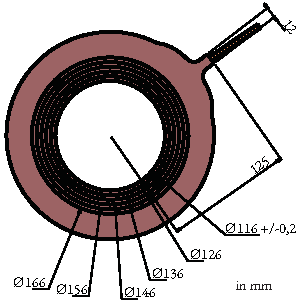
\includegraphics[]{\imagepath/single_coil_geometry_kraemer/single_coil_geometry_kraemer.pdf}
        \caption{Specified geometrical properties of the Feshbach coils. Drawing supplied by the producer (Krämer Energietechnik)}
        \label{fig:single_coil_geometry_kraemer}
    \end{subfigure}
    
    \begin{subfigure}[t]{\textwidth}
        \centering
        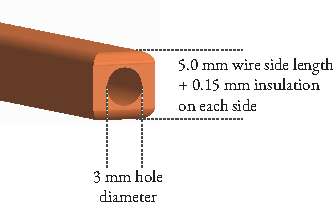
\includegraphics[]{\imagepath/wire_specification/wire_specification.pdf}
        \caption{Wire specification: The square copper wire has a side length of \SI{5.0}{\milli\meter}, the hollow core has a diameter of \SI{3.0}{\milli\meter}. On each side, a Kapton insulation layer of \SI{0.15}{\milli\meter} }
        \label{fig:wire_specification}
    \end{subfigure}
    \caption{Details of the geometrical specification of the Feshbach coils}
    \label{fig:coil_geometrical_properties}
\end{figure}



\chapter{Rules of Thumb for Magnetic Fields and Gradients}\label{ch:rules_of_thumb}
The following rules of thumb are useful for calculating the magnitude of homogeneous fields and gradients for coils in Helmholtz configuration, meaning that the distance of the coils equals their radius.

\section*{Homogeneous Fields}
The field in 
Gauss
% \href{https://www.youtube.com/watch?v=_3_JVVs2Kls}{\GaUsS}
at the center of a Helmholtz configuration of coils with radius $r$ operated at current $I$ can be estimated as
\begin{align}\label{eq:rot_field}
    B(r, I) \approx \left. \frac{I}{\SI{1}{\ampere}} \middle/ \frac{r}{\SI{1}{\centi\meter}} ~ \cdot ~\SI{1}{\gauss}\right. .
\end{align}
This means that, roughly speaking, coils in  Helmholtz configuration generate a field of
\begin{align}\nonumber
    \SI{1}{\gauss} ~~ \text{per} ~~ \frac{\si{\ampere} ~~ \text{of current}}{\si{\centi\meter} ~~ \text{of radius}}~.
\end{align}

Figure~\ref{fig:rot_field} compares this rule of thumb to exact simulations with the \textit{coil simulation library} (see~\ref{ch:simulation} and~\ref{ch:coil_simulation_library}). The rule of thumb overestimates the field by about \SI{10}{\percent}.

\begin{figure}
    \centering
    \begin{subfigure}[t]{0.48\textwidth}
        \centering
        \begin{pgfpicture}
            \pgftext{%% Creator: Matplotlib, PGF backend
%%
%% To include the figure in your LaTeX document, write
%%   \input{<filename>.pgf}
%%
%% Make sure the required packages are loaded in your preamble
%%   \usepackage{pgf}
%%
%% Also ensure that all the required font packages are loaded; for instance,
%% the lmodern package is sometimes necessary when using math font.
%%   \usepackage{lmodern}
%%
%% Figures using additional raster images can only be included by \input if
%% they are in the same directory as the main LaTeX file. For loading figures
%% from other directories you can use the `import` package
%%   \usepackage{import}
%%
%% and then include the figures with
%%   \import{<path to file>}{<filename>.pgf}
%%
%% Matplotlib used the following preamble
%%   \usepackage{fontspec}
%%   \setmainfont{DejaVuSerif.ttf}[Path=\detokenize{/home/max/.conda/envs/3d_mot/lib/python3.9/site-packages/matplotlib/mpl-data/fonts/ttf/}]
%%   \setsansfont{DejaVuSans.ttf}[Path=\detokenize{/home/max/.conda/envs/3d_mot/lib/python3.9/site-packages/matplotlib/mpl-data/fonts/ttf/}]
%%   \setmonofont{DejaVuSansMono.ttf}[Path=\detokenize{/home/max/.conda/envs/3d_mot/lib/python3.9/site-packages/matplotlib/mpl-data/fonts/ttf/}]
%%
\begingroup%
\makeatletter%
\begin{pgfpicture}%
\pgfpathrectangle{\pgfpointorigin}{\pgfqpoint{2.463516in}{1.635075in}}%
\pgfusepath{use as bounding box, clip}%
\begin{pgfscope}%
\pgfsetbuttcap%
\pgfsetmiterjoin%
\pgfsetlinewidth{0.000000pt}%
\definecolor{currentstroke}{rgb}{1.000000,1.000000,1.000000}%
\pgfsetstrokecolor{currentstroke}%
\pgfsetstrokeopacity{0.000000}%
\pgfsetdash{}{0pt}%
\pgfpathmoveto{\pgfqpoint{0.000000in}{0.000000in}}%
\pgfpathlineto{\pgfqpoint{2.463516in}{0.000000in}}%
\pgfpathlineto{\pgfqpoint{2.463516in}{1.635075in}}%
\pgfpathlineto{\pgfqpoint{0.000000in}{1.635075in}}%
\pgfpathlineto{\pgfqpoint{0.000000in}{0.000000in}}%
\pgfpathclose%
\pgfusepath{}%
\end{pgfscope}%
\begin{pgfscope}%
\pgfsetbuttcap%
\pgfsetmiterjoin%
\definecolor{currentfill}{rgb}{1.000000,1.000000,1.000000}%
\pgfsetfillcolor{currentfill}%
\pgfsetlinewidth{0.000000pt}%
\definecolor{currentstroke}{rgb}{0.000000,0.000000,0.000000}%
\pgfsetstrokecolor{currentstroke}%
\pgfsetstrokeopacity{0.000000}%
\pgfsetdash{}{0pt}%
\pgfpathmoveto{\pgfqpoint{0.532807in}{0.494721in}}%
\pgfpathlineto{\pgfqpoint{2.363516in}{0.494721in}}%
\pgfpathlineto{\pgfqpoint{2.363516in}{1.535075in}}%
\pgfpathlineto{\pgfqpoint{0.532807in}{1.535075in}}%
\pgfpathlineto{\pgfqpoint{0.532807in}{0.494721in}}%
\pgfpathclose%
\pgfusepath{fill}%
\end{pgfscope}%
\begin{pgfscope}%
\pgfpathrectangle{\pgfqpoint{0.532807in}{0.494721in}}{\pgfqpoint{1.830709in}{1.040354in}}%
\pgfusepath{clip}%
\pgfsetrectcap%
\pgfsetroundjoin%
\pgfsetlinewidth{0.803000pt}%
\definecolor{currentstroke}{rgb}{0.690196,0.690196,0.690196}%
\pgfsetstrokecolor{currentstroke}%
\pgfsetdash{}{0pt}%
\pgfpathmoveto{\pgfqpoint{0.616021in}{0.494721in}}%
\pgfpathlineto{\pgfqpoint{0.616021in}{1.535075in}}%
\pgfusepath{stroke}%
\end{pgfscope}%
\begin{pgfscope}%
\pgfsetbuttcap%
\pgfsetroundjoin%
\definecolor{currentfill}{rgb}{0.000000,0.000000,0.000000}%
\pgfsetfillcolor{currentfill}%
\pgfsetlinewidth{0.803000pt}%
\definecolor{currentstroke}{rgb}{0.000000,0.000000,0.000000}%
\pgfsetstrokecolor{currentstroke}%
\pgfsetdash{}{0pt}%
\pgfsys@defobject{currentmarker}{\pgfqpoint{0.000000in}{-0.048611in}}{\pgfqpoint{0.000000in}{0.000000in}}{%
\pgfpathmoveto{\pgfqpoint{0.000000in}{0.000000in}}%
\pgfpathlineto{\pgfqpoint{0.000000in}{-0.048611in}}%
\pgfusepath{stroke,fill}%
}%
\begin{pgfscope}%
\pgfsys@transformshift{0.616021in}{0.494721in}%
\pgfsys@useobject{currentmarker}{}%
\end{pgfscope}%
\end{pgfscope}%
\begin{pgfscope}%
\definecolor{textcolor}{rgb}{0.000000,0.000000,0.000000}%
\pgfsetstrokecolor{textcolor}%
\pgfsetfillcolor{textcolor}%
\pgftext[x=0.616021in,y=0.397499in,,top]{\color{textcolor}\rmfamily\fontsize{9.000000}{10.800000}\selectfont \ensuremath{8}}%
\end{pgfscope}%
\begin{pgfscope}%
\pgfpathrectangle{\pgfqpoint{0.532807in}{0.494721in}}{\pgfqpoint{1.830709in}{1.040354in}}%
\pgfusepath{clip}%
\pgfsetrectcap%
\pgfsetroundjoin%
\pgfsetlinewidth{0.803000pt}%
\definecolor{currentstroke}{rgb}{0.690196,0.690196,0.690196}%
\pgfsetstrokecolor{currentstroke}%
\pgfsetdash{}{0pt}%
\pgfpathmoveto{\pgfqpoint{1.032091in}{0.494721in}}%
\pgfpathlineto{\pgfqpoint{1.032091in}{1.535075in}}%
\pgfusepath{stroke}%
\end{pgfscope}%
\begin{pgfscope}%
\pgfsetbuttcap%
\pgfsetroundjoin%
\definecolor{currentfill}{rgb}{0.000000,0.000000,0.000000}%
\pgfsetfillcolor{currentfill}%
\pgfsetlinewidth{0.803000pt}%
\definecolor{currentstroke}{rgb}{0.000000,0.000000,0.000000}%
\pgfsetstrokecolor{currentstroke}%
\pgfsetdash{}{0pt}%
\pgfsys@defobject{currentmarker}{\pgfqpoint{0.000000in}{-0.048611in}}{\pgfqpoint{0.000000in}{0.000000in}}{%
\pgfpathmoveto{\pgfqpoint{0.000000in}{0.000000in}}%
\pgfpathlineto{\pgfqpoint{0.000000in}{-0.048611in}}%
\pgfusepath{stroke,fill}%
}%
\begin{pgfscope}%
\pgfsys@transformshift{1.032091in}{0.494721in}%
\pgfsys@useobject{currentmarker}{}%
\end{pgfscope}%
\end{pgfscope}%
\begin{pgfscope}%
\definecolor{textcolor}{rgb}{0.000000,0.000000,0.000000}%
\pgfsetstrokecolor{textcolor}%
\pgfsetfillcolor{textcolor}%
\pgftext[x=1.032091in,y=0.397499in,,top]{\color{textcolor}\rmfamily\fontsize{9.000000}{10.800000}\selectfont \ensuremath{9}}%
\end{pgfscope}%
\begin{pgfscope}%
\pgfpathrectangle{\pgfqpoint{0.532807in}{0.494721in}}{\pgfqpoint{1.830709in}{1.040354in}}%
\pgfusepath{clip}%
\pgfsetrectcap%
\pgfsetroundjoin%
\pgfsetlinewidth{0.803000pt}%
\definecolor{currentstroke}{rgb}{0.690196,0.690196,0.690196}%
\pgfsetstrokecolor{currentstroke}%
\pgfsetdash{}{0pt}%
\pgfpathmoveto{\pgfqpoint{1.448161in}{0.494721in}}%
\pgfpathlineto{\pgfqpoint{1.448161in}{1.535075in}}%
\pgfusepath{stroke}%
\end{pgfscope}%
\begin{pgfscope}%
\pgfsetbuttcap%
\pgfsetroundjoin%
\definecolor{currentfill}{rgb}{0.000000,0.000000,0.000000}%
\pgfsetfillcolor{currentfill}%
\pgfsetlinewidth{0.803000pt}%
\definecolor{currentstroke}{rgb}{0.000000,0.000000,0.000000}%
\pgfsetstrokecolor{currentstroke}%
\pgfsetdash{}{0pt}%
\pgfsys@defobject{currentmarker}{\pgfqpoint{0.000000in}{-0.048611in}}{\pgfqpoint{0.000000in}{0.000000in}}{%
\pgfpathmoveto{\pgfqpoint{0.000000in}{0.000000in}}%
\pgfpathlineto{\pgfqpoint{0.000000in}{-0.048611in}}%
\pgfusepath{stroke,fill}%
}%
\begin{pgfscope}%
\pgfsys@transformshift{1.448161in}{0.494721in}%
\pgfsys@useobject{currentmarker}{}%
\end{pgfscope}%
\end{pgfscope}%
\begin{pgfscope}%
\definecolor{textcolor}{rgb}{0.000000,0.000000,0.000000}%
\pgfsetstrokecolor{textcolor}%
\pgfsetfillcolor{textcolor}%
\pgftext[x=1.448161in,y=0.397499in,,top]{\color{textcolor}\rmfamily\fontsize{9.000000}{10.800000}\selectfont \ensuremath{10}}%
\end{pgfscope}%
\begin{pgfscope}%
\pgfpathrectangle{\pgfqpoint{0.532807in}{0.494721in}}{\pgfqpoint{1.830709in}{1.040354in}}%
\pgfusepath{clip}%
\pgfsetrectcap%
\pgfsetroundjoin%
\pgfsetlinewidth{0.803000pt}%
\definecolor{currentstroke}{rgb}{0.690196,0.690196,0.690196}%
\pgfsetstrokecolor{currentstroke}%
\pgfsetdash{}{0pt}%
\pgfpathmoveto{\pgfqpoint{1.864231in}{0.494721in}}%
\pgfpathlineto{\pgfqpoint{1.864231in}{1.535075in}}%
\pgfusepath{stroke}%
\end{pgfscope}%
\begin{pgfscope}%
\pgfsetbuttcap%
\pgfsetroundjoin%
\definecolor{currentfill}{rgb}{0.000000,0.000000,0.000000}%
\pgfsetfillcolor{currentfill}%
\pgfsetlinewidth{0.803000pt}%
\definecolor{currentstroke}{rgb}{0.000000,0.000000,0.000000}%
\pgfsetstrokecolor{currentstroke}%
\pgfsetdash{}{0pt}%
\pgfsys@defobject{currentmarker}{\pgfqpoint{0.000000in}{-0.048611in}}{\pgfqpoint{0.000000in}{0.000000in}}{%
\pgfpathmoveto{\pgfqpoint{0.000000in}{0.000000in}}%
\pgfpathlineto{\pgfqpoint{0.000000in}{-0.048611in}}%
\pgfusepath{stroke,fill}%
}%
\begin{pgfscope}%
\pgfsys@transformshift{1.864231in}{0.494721in}%
\pgfsys@useobject{currentmarker}{}%
\end{pgfscope}%
\end{pgfscope}%
\begin{pgfscope}%
\definecolor{textcolor}{rgb}{0.000000,0.000000,0.000000}%
\pgfsetstrokecolor{textcolor}%
\pgfsetfillcolor{textcolor}%
\pgftext[x=1.864231in,y=0.397499in,,top]{\color{textcolor}\rmfamily\fontsize{9.000000}{10.800000}\selectfont \ensuremath{11}}%
\end{pgfscope}%
\begin{pgfscope}%
\pgfpathrectangle{\pgfqpoint{0.532807in}{0.494721in}}{\pgfqpoint{1.830709in}{1.040354in}}%
\pgfusepath{clip}%
\pgfsetrectcap%
\pgfsetroundjoin%
\pgfsetlinewidth{0.803000pt}%
\definecolor{currentstroke}{rgb}{0.690196,0.690196,0.690196}%
\pgfsetstrokecolor{currentstroke}%
\pgfsetdash{}{0pt}%
\pgfpathmoveto{\pgfqpoint{2.280302in}{0.494721in}}%
\pgfpathlineto{\pgfqpoint{2.280302in}{1.535075in}}%
\pgfusepath{stroke}%
\end{pgfscope}%
\begin{pgfscope}%
\pgfsetbuttcap%
\pgfsetroundjoin%
\definecolor{currentfill}{rgb}{0.000000,0.000000,0.000000}%
\pgfsetfillcolor{currentfill}%
\pgfsetlinewidth{0.803000pt}%
\definecolor{currentstroke}{rgb}{0.000000,0.000000,0.000000}%
\pgfsetstrokecolor{currentstroke}%
\pgfsetdash{}{0pt}%
\pgfsys@defobject{currentmarker}{\pgfqpoint{0.000000in}{-0.048611in}}{\pgfqpoint{0.000000in}{0.000000in}}{%
\pgfpathmoveto{\pgfqpoint{0.000000in}{0.000000in}}%
\pgfpathlineto{\pgfqpoint{0.000000in}{-0.048611in}}%
\pgfusepath{stroke,fill}%
}%
\begin{pgfscope}%
\pgfsys@transformshift{2.280302in}{0.494721in}%
\pgfsys@useobject{currentmarker}{}%
\end{pgfscope}%
\end{pgfscope}%
\begin{pgfscope}%
\definecolor{textcolor}{rgb}{0.000000,0.000000,0.000000}%
\pgfsetstrokecolor{textcolor}%
\pgfsetfillcolor{textcolor}%
\pgftext[x=2.280302in,y=0.397499in,,top]{\color{textcolor}\rmfamily\fontsize{9.000000}{10.800000}\selectfont \ensuremath{12}}%
\end{pgfscope}%
\begin{pgfscope}%
\definecolor{textcolor}{rgb}{0.000000,0.000000,0.000000}%
\pgfsetstrokecolor{textcolor}%
\pgfsetfillcolor{textcolor}%
\pgftext[x=1.448161in,y=0.220972in,,top]{\color{textcolor}\rmfamily\fontsize{9.000000}{10.800000}\selectfont radius in cm}%
\end{pgfscope}%
\begin{pgfscope}%
\pgfpathrectangle{\pgfqpoint{0.532807in}{0.494721in}}{\pgfqpoint{1.830709in}{1.040354in}}%
\pgfusepath{clip}%
\pgfsetrectcap%
\pgfsetroundjoin%
\pgfsetlinewidth{0.803000pt}%
\definecolor{currentstroke}{rgb}{0.690196,0.690196,0.690196}%
\pgfsetstrokecolor{currentstroke}%
\pgfsetdash{}{0pt}%
\pgfpathmoveto{\pgfqpoint{0.532807in}{0.637754in}}%
\pgfpathlineto{\pgfqpoint{2.363516in}{0.637754in}}%
\pgfusepath{stroke}%
\end{pgfscope}%
\begin{pgfscope}%
\pgfsetbuttcap%
\pgfsetroundjoin%
\definecolor{currentfill}{rgb}{0.000000,0.000000,0.000000}%
\pgfsetfillcolor{currentfill}%
\pgfsetlinewidth{0.803000pt}%
\definecolor{currentstroke}{rgb}{0.000000,0.000000,0.000000}%
\pgfsetstrokecolor{currentstroke}%
\pgfsetdash{}{0pt}%
\pgfsys@defobject{currentmarker}{\pgfqpoint{-0.048611in}{0.000000in}}{\pgfqpoint{-0.000000in}{0.000000in}}{%
\pgfpathmoveto{\pgfqpoint{-0.000000in}{0.000000in}}%
\pgfpathlineto{\pgfqpoint{-0.048611in}{0.000000in}}%
\pgfusepath{stroke,fill}%
}%
\begin{pgfscope}%
\pgfsys@transformshift{0.532807in}{0.637754in}%
\pgfsys@useobject{currentmarker}{}%
\end{pgfscope}%
\end{pgfscope}%
\begin{pgfscope}%
\definecolor{textcolor}{rgb}{0.000000,0.000000,0.000000}%
\pgfsetstrokecolor{textcolor}%
\pgfsetfillcolor{textcolor}%
\pgftext[x=0.356056in, y=0.590269in, left, base]{\color{textcolor}\rmfamily\fontsize{9.000000}{10.800000}\selectfont \ensuremath{8}}%
\end{pgfscope}%
\begin{pgfscope}%
\pgfpathrectangle{\pgfqpoint{0.532807in}{0.494721in}}{\pgfqpoint{1.830709in}{1.040354in}}%
\pgfusepath{clip}%
\pgfsetrectcap%
\pgfsetroundjoin%
\pgfsetlinewidth{0.803000pt}%
\definecolor{currentstroke}{rgb}{0.690196,0.690196,0.690196}%
\pgfsetstrokecolor{currentstroke}%
\pgfsetdash{}{0pt}%
\pgfpathmoveto{\pgfqpoint{0.532807in}{1.015546in}}%
\pgfpathlineto{\pgfqpoint{2.363516in}{1.015546in}}%
\pgfusepath{stroke}%
\end{pgfscope}%
\begin{pgfscope}%
\pgfsetbuttcap%
\pgfsetroundjoin%
\definecolor{currentfill}{rgb}{0.000000,0.000000,0.000000}%
\pgfsetfillcolor{currentfill}%
\pgfsetlinewidth{0.803000pt}%
\definecolor{currentstroke}{rgb}{0.000000,0.000000,0.000000}%
\pgfsetstrokecolor{currentstroke}%
\pgfsetdash{}{0pt}%
\pgfsys@defobject{currentmarker}{\pgfqpoint{-0.048611in}{0.000000in}}{\pgfqpoint{-0.000000in}{0.000000in}}{%
\pgfpathmoveto{\pgfqpoint{-0.000000in}{0.000000in}}%
\pgfpathlineto{\pgfqpoint{-0.048611in}{0.000000in}}%
\pgfusepath{stroke,fill}%
}%
\begin{pgfscope}%
\pgfsys@transformshift{0.532807in}{1.015546in}%
\pgfsys@useobject{currentmarker}{}%
\end{pgfscope}%
\end{pgfscope}%
\begin{pgfscope}%
\definecolor{textcolor}{rgb}{0.000000,0.000000,0.000000}%
\pgfsetstrokecolor{textcolor}%
\pgfsetfillcolor{textcolor}%
\pgftext[x=0.276527in, y=0.968061in, left, base]{\color{textcolor}\rmfamily\fontsize{9.000000}{10.800000}\selectfont \ensuremath{10}}%
\end{pgfscope}%
\begin{pgfscope}%
\pgfpathrectangle{\pgfqpoint{0.532807in}{0.494721in}}{\pgfqpoint{1.830709in}{1.040354in}}%
\pgfusepath{clip}%
\pgfsetrectcap%
\pgfsetroundjoin%
\pgfsetlinewidth{0.803000pt}%
\definecolor{currentstroke}{rgb}{0.690196,0.690196,0.690196}%
\pgfsetstrokecolor{currentstroke}%
\pgfsetdash{}{0pt}%
\pgfpathmoveto{\pgfqpoint{0.532807in}{1.393338in}}%
\pgfpathlineto{\pgfqpoint{2.363516in}{1.393338in}}%
\pgfusepath{stroke}%
\end{pgfscope}%
\begin{pgfscope}%
\pgfsetbuttcap%
\pgfsetroundjoin%
\definecolor{currentfill}{rgb}{0.000000,0.000000,0.000000}%
\pgfsetfillcolor{currentfill}%
\pgfsetlinewidth{0.803000pt}%
\definecolor{currentstroke}{rgb}{0.000000,0.000000,0.000000}%
\pgfsetstrokecolor{currentstroke}%
\pgfsetdash{}{0pt}%
\pgfsys@defobject{currentmarker}{\pgfqpoint{-0.048611in}{0.000000in}}{\pgfqpoint{-0.000000in}{0.000000in}}{%
\pgfpathmoveto{\pgfqpoint{-0.000000in}{0.000000in}}%
\pgfpathlineto{\pgfqpoint{-0.048611in}{0.000000in}}%
\pgfusepath{stroke,fill}%
}%
\begin{pgfscope}%
\pgfsys@transformshift{0.532807in}{1.393338in}%
\pgfsys@useobject{currentmarker}{}%
\end{pgfscope}%
\end{pgfscope}%
\begin{pgfscope}%
\definecolor{textcolor}{rgb}{0.000000,0.000000,0.000000}%
\pgfsetstrokecolor{textcolor}%
\pgfsetfillcolor{textcolor}%
\pgftext[x=0.276527in, y=1.345853in, left, base]{\color{textcolor}\rmfamily\fontsize{9.000000}{10.800000}\selectfont \ensuremath{12}}%
\end{pgfscope}%
\begin{pgfscope}%
\definecolor{textcolor}{rgb}{0.000000,0.000000,0.000000}%
\pgfsetstrokecolor{textcolor}%
\pgfsetfillcolor{textcolor}%
\pgftext[x=0.220972in,y=1.014898in,,bottom,rotate=90.000000]{\color{textcolor}\rmfamily\fontsize{9.000000}{10.800000}\selectfont field in G}%
\end{pgfscope}%
\begin{pgfscope}%
\pgfpathrectangle{\pgfqpoint{0.532807in}{0.494721in}}{\pgfqpoint{1.830709in}{1.040354in}}%
\pgfusepath{clip}%
\pgfsetrectcap%
\pgfsetroundjoin%
\pgfsetlinewidth{1.505625pt}%
\definecolor{currentstroke}{rgb}{1.000000,0.000000,0.000000}%
\pgfsetstrokecolor{currentstroke}%
\pgfsetdash{}{0pt}%
\pgfpathmoveto{\pgfqpoint{0.616021in}{1.249721in}}%
\pgfpathlineto{\pgfqpoint{0.703615in}{1.195282in}}%
\pgfpathlineto{\pgfqpoint{0.791208in}{1.143565in}}%
\pgfpathlineto{\pgfqpoint{0.878802in}{1.094370in}}%
\pgfpathlineto{\pgfqpoint{0.966396in}{1.047518in}}%
\pgfpathlineto{\pgfqpoint{1.053990in}{1.002845in}}%
\pgfpathlineto{\pgfqpoint{1.141583in}{0.960203in}}%
\pgfpathlineto{\pgfqpoint{1.229177in}{0.919456in}}%
\pgfpathlineto{\pgfqpoint{1.316771in}{0.880480in}}%
\pgfpathlineto{\pgfqpoint{1.404364in}{0.843164in}}%
\pgfpathlineto{\pgfqpoint{1.491958in}{0.807402in}}%
\pgfpathlineto{\pgfqpoint{1.579552in}{0.773099in}}%
\pgfpathlineto{\pgfqpoint{1.667146in}{0.740169in}}%
\pgfpathlineto{\pgfqpoint{1.754739in}{0.708530in}}%
\pgfpathlineto{\pgfqpoint{1.842333in}{0.678108in}}%
\pgfpathlineto{\pgfqpoint{1.929927in}{0.648834in}}%
\pgfpathlineto{\pgfqpoint{2.017520in}{0.620644in}}%
\pgfpathlineto{\pgfqpoint{2.105114in}{0.593480in}}%
\pgfpathlineto{\pgfqpoint{2.192708in}{0.567285in}}%
\pgfpathlineto{\pgfqpoint{2.280302in}{0.542010in}}%
\pgfusepath{stroke}%
\end{pgfscope}%
\begin{pgfscope}%
\pgfpathrectangle{\pgfqpoint{0.532807in}{0.494721in}}{\pgfqpoint{1.830709in}{1.040354in}}%
\pgfusepath{clip}%
\pgfsetrectcap%
\pgfsetroundjoin%
\pgfsetlinewidth{1.505625pt}%
\definecolor{currentstroke}{rgb}{0.278431,0.282353,0.278431}%
\pgfsetstrokecolor{currentstroke}%
\pgfsetdash{}{0pt}%
\pgfpathmoveto{\pgfqpoint{0.616021in}{1.487786in}}%
\pgfpathlineto{\pgfqpoint{0.703615in}{1.427243in}}%
\pgfpathlineto{\pgfqpoint{0.791208in}{1.369726in}}%
\pgfpathlineto{\pgfqpoint{0.878802in}{1.315016in}}%
\pgfpathlineto{\pgfqpoint{0.966396in}{1.262910in}}%
\pgfpathlineto{\pgfqpoint{1.053990in}{1.213228in}}%
\pgfpathlineto{\pgfqpoint{1.141583in}{1.165805in}}%
\pgfpathlineto{\pgfqpoint{1.229177in}{1.120489in}}%
\pgfpathlineto{\pgfqpoint{1.316771in}{1.077143in}}%
\pgfpathlineto{\pgfqpoint{1.404364in}{1.035642in}}%
\pgfpathlineto{\pgfqpoint{1.491958in}{0.995870in}}%
\pgfpathlineto{\pgfqpoint{1.579552in}{0.957721in}}%
\pgfpathlineto{\pgfqpoint{1.667146in}{0.921098in}}%
\pgfpathlineto{\pgfqpoint{1.754739in}{0.885912in}}%
\pgfpathlineto{\pgfqpoint{1.842333in}{0.852079in}}%
\pgfpathlineto{\pgfqpoint{1.929927in}{0.819522in}}%
\pgfpathlineto{\pgfqpoint{2.017520in}{0.788171in}}%
\pgfpathlineto{\pgfqpoint{2.105114in}{0.757961in}}%
\pgfpathlineto{\pgfqpoint{2.192708in}{0.728829in}}%
\pgfpathlineto{\pgfqpoint{2.280302in}{0.700720in}}%
\pgfusepath{stroke}%
\end{pgfscope}%
\begin{pgfscope}%
\pgfsetrectcap%
\pgfsetmiterjoin%
\pgfsetlinewidth{0.803000pt}%
\definecolor{currentstroke}{rgb}{0.000000,0.000000,0.000000}%
\pgfsetstrokecolor{currentstroke}%
\pgfsetdash{}{0pt}%
\pgfpathmoveto{\pgfqpoint{0.532807in}{0.494721in}}%
\pgfpathlineto{\pgfqpoint{0.532807in}{1.535075in}}%
\pgfusepath{stroke}%
\end{pgfscope}%
\begin{pgfscope}%
\pgfsetrectcap%
\pgfsetmiterjoin%
\pgfsetlinewidth{0.803000pt}%
\definecolor{currentstroke}{rgb}{0.000000,0.000000,0.000000}%
\pgfsetstrokecolor{currentstroke}%
\pgfsetdash{}{0pt}%
\pgfpathmoveto{\pgfqpoint{2.363516in}{0.494721in}}%
\pgfpathlineto{\pgfqpoint{2.363516in}{1.535075in}}%
\pgfusepath{stroke}%
\end{pgfscope}%
\begin{pgfscope}%
\pgfsetrectcap%
\pgfsetmiterjoin%
\pgfsetlinewidth{0.803000pt}%
\definecolor{currentstroke}{rgb}{0.000000,0.000000,0.000000}%
\pgfsetstrokecolor{currentstroke}%
\pgfsetdash{}{0pt}%
\pgfpathmoveto{\pgfqpoint{0.532807in}{0.494721in}}%
\pgfpathlineto{\pgfqpoint{2.363516in}{0.494721in}}%
\pgfusepath{stroke}%
\end{pgfscope}%
\begin{pgfscope}%
\pgfsetrectcap%
\pgfsetmiterjoin%
\pgfsetlinewidth{0.803000pt}%
\definecolor{currentstroke}{rgb}{0.000000,0.000000,0.000000}%
\pgfsetstrokecolor{currentstroke}%
\pgfsetdash{}{0pt}%
\pgfpathmoveto{\pgfqpoint{0.532807in}{1.535075in}}%
\pgfpathlineto{\pgfqpoint{2.363516in}{1.535075in}}%
\pgfusepath{stroke}%
\end{pgfscope}%
\begin{pgfscope}%
\pgfsetbuttcap%
\pgfsetmiterjoin%
\definecolor{currentfill}{rgb}{1.000000,1.000000,1.000000}%
\pgfsetfillcolor{currentfill}%
\pgfsetfillopacity{0.800000}%
\pgfsetlinewidth{1.003750pt}%
\definecolor{currentstroke}{rgb}{0.800000,0.800000,0.800000}%
\pgfsetstrokecolor{currentstroke}%
\pgfsetstrokeopacity{0.800000}%
\pgfsetdash{}{0pt}%
\pgfpathmoveto{\pgfqpoint{1.461855in}{1.223780in}}%
\pgfpathlineto{\pgfqpoint{2.305182in}{1.223780in}}%
\pgfpathquadraticcurveto{\pgfqpoint{2.321849in}{1.223780in}}{\pgfqpoint{2.321849in}{1.240447in}}%
\pgfpathlineto{\pgfqpoint{2.321849in}{1.476742in}}%
\pgfpathquadraticcurveto{\pgfqpoint{2.321849in}{1.493408in}}{\pgfqpoint{2.305182in}{1.493408in}}%
\pgfpathlineto{\pgfqpoint{1.461855in}{1.493408in}}%
\pgfpathquadraticcurveto{\pgfqpoint{1.445189in}{1.493408in}}{\pgfqpoint{1.445189in}{1.476742in}}%
\pgfpathlineto{\pgfqpoint{1.445189in}{1.240447in}}%
\pgfpathquadraticcurveto{\pgfqpoint{1.445189in}{1.223780in}}{\pgfqpoint{1.461855in}{1.223780in}}%
\pgfpathlineto{\pgfqpoint{1.461855in}{1.223780in}}%
\pgfpathclose%
\pgfusepath{stroke,fill}%
\end{pgfscope}%
\begin{pgfscope}%
\pgfsetrectcap%
\pgfsetroundjoin%
\pgfsetlinewidth{1.505625pt}%
\definecolor{currentstroke}{rgb}{1.000000,0.000000,0.000000}%
\pgfsetstrokecolor{currentstroke}%
\pgfsetdash{}{0pt}%
\pgfpathmoveto{\pgfqpoint{1.478522in}{1.425928in}}%
\pgfpathlineto{\pgfqpoint{1.561855in}{1.425928in}}%
\pgfpathlineto{\pgfqpoint{1.645189in}{1.425928in}}%
\pgfusepath{stroke}%
\end{pgfscope}%
\begin{pgfscope}%
\definecolor{textcolor}{rgb}{0.000000,0.000000,0.000000}%
\pgfsetstrokecolor{textcolor}%
\pgfsetfillcolor{textcolor}%
\pgftext[x=1.711855in,y=1.396761in,left,base]{\color{textcolor}\rmfamily\fontsize{6.000000}{7.200000}\selectfont field}%
\end{pgfscope}%
\begin{pgfscope}%
\pgfsetrectcap%
\pgfsetroundjoin%
\pgfsetlinewidth{1.505625pt}%
\definecolor{currentstroke}{rgb}{0.278431,0.282353,0.278431}%
\pgfsetstrokecolor{currentstroke}%
\pgfsetdash{}{0pt}%
\pgfpathmoveto{\pgfqpoint{1.478522in}{1.303614in}}%
\pgfpathlineto{\pgfqpoint{1.561855in}{1.303614in}}%
\pgfpathlineto{\pgfqpoint{1.645189in}{1.303614in}}%
\pgfusepath{stroke}%
\end{pgfscope}%
\begin{pgfscope}%
\definecolor{textcolor}{rgb}{0.000000,0.000000,0.000000}%
\pgfsetstrokecolor{textcolor}%
\pgfsetfillcolor{textcolor}%
\pgftext[x=1.711855in,y=1.274447in,left,base]{\color{textcolor}\rmfamily\fontsize{6.000000}{7.200000}\selectfont rule of thumb}%
\end{pgfscope}%
\end{pgfpicture}%
\makeatother%
\endgroup%
}
        \end{pgfpicture}
        \caption{Dependency on the radius, with the coil distance fixed to the radius}
        \label{fig:rot_field_radius}
    \end{subfigure} 
    \hspace{0.03\textwidth}
    \begin{subfigure}[t]{0.48\textwidth}
        \centering
        \begin{pgfpicture}
            \pgftext{%% Creator: Matplotlib, PGF backend
%%
%% To include the figure in your LaTeX document, write
%%   \input{<filename>.pgf}
%%
%% Make sure the required packages are loaded in your preamble
%%   \usepackage{pgf}
%%
%% Also ensure that all the required font packages are loaded; for instance,
%% the lmodern package is sometimes necessary when using math font.
%%   \usepackage{lmodern}
%%
%% Figures using additional raster images can only be included by \input if
%% they are in the same directory as the main LaTeX file. For loading figures
%% from other directories you can use the `import` package
%%   \usepackage{import}
%%
%% and then include the figures with
%%   \import{<path to file>}{<filename>.pgf}
%%
%% Matplotlib used the following preamble
%%   \usepackage{fontspec}
%%   \setmainfont{DejaVuSerif.ttf}[Path=\detokenize{/home/max/.conda/envs/3d_mot/lib/python3.9/site-packages/matplotlib/mpl-data/fonts/ttf/}]
%%   \setsansfont{DejaVuSans.ttf}[Path=\detokenize{/home/max/.conda/envs/3d_mot/lib/python3.9/site-packages/matplotlib/mpl-data/fonts/ttf/}]
%%   \setmonofont{DejaVuSansMono.ttf}[Path=\detokenize{/home/max/.conda/envs/3d_mot/lib/python3.9/site-packages/matplotlib/mpl-data/fonts/ttf/}]
%%
\begingroup%
\makeatletter%
\begin{pgfpicture}%
\pgfpathrectangle{\pgfpointorigin}{\pgfqpoint{2.499595in}{1.635272in}}%
\pgfusepath{use as bounding box, clip}%
\begin{pgfscope}%
\pgfsetbuttcap%
\pgfsetmiterjoin%
\pgfsetlinewidth{0.000000pt}%
\definecolor{currentstroke}{rgb}{1.000000,1.000000,1.000000}%
\pgfsetstrokecolor{currentstroke}%
\pgfsetstrokeopacity{0.000000}%
\pgfsetdash{}{0pt}%
\pgfpathmoveto{\pgfqpoint{0.000000in}{0.000000in}}%
\pgfpathlineto{\pgfqpoint{2.499595in}{0.000000in}}%
\pgfpathlineto{\pgfqpoint{2.499595in}{1.635272in}}%
\pgfpathlineto{\pgfqpoint{0.000000in}{1.635272in}}%
\pgfpathlineto{\pgfqpoint{0.000000in}{0.000000in}}%
\pgfpathclose%
\pgfusepath{}%
\end{pgfscope}%
\begin{pgfscope}%
\pgfsetbuttcap%
\pgfsetmiterjoin%
\definecolor{currentfill}{rgb}{1.000000,1.000000,1.000000}%
\pgfsetfillcolor{currentfill}%
\pgfsetlinewidth{0.000000pt}%
\definecolor{currentstroke}{rgb}{0.000000,0.000000,0.000000}%
\pgfsetstrokecolor{currentstroke}%
\pgfsetstrokeopacity{0.000000}%
\pgfsetdash{}{0pt}%
\pgfpathmoveto{\pgfqpoint{0.532807in}{0.494721in}}%
\pgfpathlineto{\pgfqpoint{2.363516in}{0.494721in}}%
\pgfpathlineto{\pgfqpoint{2.363516in}{1.535075in}}%
\pgfpathlineto{\pgfqpoint{0.532807in}{1.535075in}}%
\pgfpathlineto{\pgfqpoint{0.532807in}{0.494721in}}%
\pgfpathclose%
\pgfusepath{fill}%
\end{pgfscope}%
\begin{pgfscope}%
\pgfpathrectangle{\pgfqpoint{0.532807in}{0.494721in}}{\pgfqpoint{1.830709in}{1.040354in}}%
\pgfusepath{clip}%
\pgfsetrectcap%
\pgfsetroundjoin%
\pgfsetlinewidth{0.803000pt}%
\definecolor{currentstroke}{rgb}{0.690196,0.690196,0.690196}%
\pgfsetstrokecolor{currentstroke}%
\pgfsetdash{}{0pt}%
\pgfpathmoveto{\pgfqpoint{0.616021in}{0.494721in}}%
\pgfpathlineto{\pgfqpoint{0.616021in}{1.535075in}}%
\pgfusepath{stroke}%
\end{pgfscope}%
\begin{pgfscope}%
\pgfsetbuttcap%
\pgfsetroundjoin%
\definecolor{currentfill}{rgb}{0.000000,0.000000,0.000000}%
\pgfsetfillcolor{currentfill}%
\pgfsetlinewidth{0.803000pt}%
\definecolor{currentstroke}{rgb}{0.000000,0.000000,0.000000}%
\pgfsetstrokecolor{currentstroke}%
\pgfsetdash{}{0pt}%
\pgfsys@defobject{currentmarker}{\pgfqpoint{0.000000in}{-0.048611in}}{\pgfqpoint{0.000000in}{0.000000in}}{%
\pgfpathmoveto{\pgfqpoint{0.000000in}{0.000000in}}%
\pgfpathlineto{\pgfqpoint{0.000000in}{-0.048611in}}%
\pgfusepath{stroke,fill}%
}%
\begin{pgfscope}%
\pgfsys@transformshift{0.616021in}{0.494721in}%
\pgfsys@useobject{currentmarker}{}%
\end{pgfscope}%
\end{pgfscope}%
\begin{pgfscope}%
\definecolor{textcolor}{rgb}{0.000000,0.000000,0.000000}%
\pgfsetstrokecolor{textcolor}%
\pgfsetfillcolor{textcolor}%
\pgftext[x=0.616021in,y=0.397499in,,top]{\color{textcolor}\rmfamily\fontsize{9.000000}{10.800000}\selectfont \ensuremath{80}}%
\end{pgfscope}%
\begin{pgfscope}%
\pgfpathrectangle{\pgfqpoint{0.532807in}{0.494721in}}{\pgfqpoint{1.830709in}{1.040354in}}%
\pgfusepath{clip}%
\pgfsetrectcap%
\pgfsetroundjoin%
\pgfsetlinewidth{0.803000pt}%
\definecolor{currentstroke}{rgb}{0.690196,0.690196,0.690196}%
\pgfsetstrokecolor{currentstroke}%
\pgfsetdash{}{0pt}%
\pgfpathmoveto{\pgfqpoint{1.032091in}{0.494721in}}%
\pgfpathlineto{\pgfqpoint{1.032091in}{1.535075in}}%
\pgfusepath{stroke}%
\end{pgfscope}%
\begin{pgfscope}%
\pgfsetbuttcap%
\pgfsetroundjoin%
\definecolor{currentfill}{rgb}{0.000000,0.000000,0.000000}%
\pgfsetfillcolor{currentfill}%
\pgfsetlinewidth{0.803000pt}%
\definecolor{currentstroke}{rgb}{0.000000,0.000000,0.000000}%
\pgfsetstrokecolor{currentstroke}%
\pgfsetdash{}{0pt}%
\pgfsys@defobject{currentmarker}{\pgfqpoint{0.000000in}{-0.048611in}}{\pgfqpoint{0.000000in}{0.000000in}}{%
\pgfpathmoveto{\pgfqpoint{0.000000in}{0.000000in}}%
\pgfpathlineto{\pgfqpoint{0.000000in}{-0.048611in}}%
\pgfusepath{stroke,fill}%
}%
\begin{pgfscope}%
\pgfsys@transformshift{1.032091in}{0.494721in}%
\pgfsys@useobject{currentmarker}{}%
\end{pgfscope}%
\end{pgfscope}%
\begin{pgfscope}%
\definecolor{textcolor}{rgb}{0.000000,0.000000,0.000000}%
\pgfsetstrokecolor{textcolor}%
\pgfsetfillcolor{textcolor}%
\pgftext[x=1.032091in,y=0.397499in,,top]{\color{textcolor}\rmfamily\fontsize{9.000000}{10.800000}\selectfont \ensuremath{90}}%
\end{pgfscope}%
\begin{pgfscope}%
\pgfpathrectangle{\pgfqpoint{0.532807in}{0.494721in}}{\pgfqpoint{1.830709in}{1.040354in}}%
\pgfusepath{clip}%
\pgfsetrectcap%
\pgfsetroundjoin%
\pgfsetlinewidth{0.803000pt}%
\definecolor{currentstroke}{rgb}{0.690196,0.690196,0.690196}%
\pgfsetstrokecolor{currentstroke}%
\pgfsetdash{}{0pt}%
\pgfpathmoveto{\pgfqpoint{1.448161in}{0.494721in}}%
\pgfpathlineto{\pgfqpoint{1.448161in}{1.535075in}}%
\pgfusepath{stroke}%
\end{pgfscope}%
\begin{pgfscope}%
\pgfsetbuttcap%
\pgfsetroundjoin%
\definecolor{currentfill}{rgb}{0.000000,0.000000,0.000000}%
\pgfsetfillcolor{currentfill}%
\pgfsetlinewidth{0.803000pt}%
\definecolor{currentstroke}{rgb}{0.000000,0.000000,0.000000}%
\pgfsetstrokecolor{currentstroke}%
\pgfsetdash{}{0pt}%
\pgfsys@defobject{currentmarker}{\pgfqpoint{0.000000in}{-0.048611in}}{\pgfqpoint{0.000000in}{0.000000in}}{%
\pgfpathmoveto{\pgfqpoint{0.000000in}{0.000000in}}%
\pgfpathlineto{\pgfqpoint{0.000000in}{-0.048611in}}%
\pgfusepath{stroke,fill}%
}%
\begin{pgfscope}%
\pgfsys@transformshift{1.448161in}{0.494721in}%
\pgfsys@useobject{currentmarker}{}%
\end{pgfscope}%
\end{pgfscope}%
\begin{pgfscope}%
\definecolor{textcolor}{rgb}{0.000000,0.000000,0.000000}%
\pgfsetstrokecolor{textcolor}%
\pgfsetfillcolor{textcolor}%
\pgftext[x=1.448161in,y=0.397499in,,top]{\color{textcolor}\rmfamily\fontsize{9.000000}{10.800000}\selectfont \ensuremath{100}}%
\end{pgfscope}%
\begin{pgfscope}%
\pgfpathrectangle{\pgfqpoint{0.532807in}{0.494721in}}{\pgfqpoint{1.830709in}{1.040354in}}%
\pgfusepath{clip}%
\pgfsetrectcap%
\pgfsetroundjoin%
\pgfsetlinewidth{0.803000pt}%
\definecolor{currentstroke}{rgb}{0.690196,0.690196,0.690196}%
\pgfsetstrokecolor{currentstroke}%
\pgfsetdash{}{0pt}%
\pgfpathmoveto{\pgfqpoint{1.864231in}{0.494721in}}%
\pgfpathlineto{\pgfqpoint{1.864231in}{1.535075in}}%
\pgfusepath{stroke}%
\end{pgfscope}%
\begin{pgfscope}%
\pgfsetbuttcap%
\pgfsetroundjoin%
\definecolor{currentfill}{rgb}{0.000000,0.000000,0.000000}%
\pgfsetfillcolor{currentfill}%
\pgfsetlinewidth{0.803000pt}%
\definecolor{currentstroke}{rgb}{0.000000,0.000000,0.000000}%
\pgfsetstrokecolor{currentstroke}%
\pgfsetdash{}{0pt}%
\pgfsys@defobject{currentmarker}{\pgfqpoint{0.000000in}{-0.048611in}}{\pgfqpoint{0.000000in}{0.000000in}}{%
\pgfpathmoveto{\pgfqpoint{0.000000in}{0.000000in}}%
\pgfpathlineto{\pgfqpoint{0.000000in}{-0.048611in}}%
\pgfusepath{stroke,fill}%
}%
\begin{pgfscope}%
\pgfsys@transformshift{1.864231in}{0.494721in}%
\pgfsys@useobject{currentmarker}{}%
\end{pgfscope}%
\end{pgfscope}%
\begin{pgfscope}%
\definecolor{textcolor}{rgb}{0.000000,0.000000,0.000000}%
\pgfsetstrokecolor{textcolor}%
\pgfsetfillcolor{textcolor}%
\pgftext[x=1.864231in,y=0.397499in,,top]{\color{textcolor}\rmfamily\fontsize{9.000000}{10.800000}\selectfont \ensuremath{110}}%
\end{pgfscope}%
\begin{pgfscope}%
\pgfpathrectangle{\pgfqpoint{0.532807in}{0.494721in}}{\pgfqpoint{1.830709in}{1.040354in}}%
\pgfusepath{clip}%
\pgfsetrectcap%
\pgfsetroundjoin%
\pgfsetlinewidth{0.803000pt}%
\definecolor{currentstroke}{rgb}{0.690196,0.690196,0.690196}%
\pgfsetstrokecolor{currentstroke}%
\pgfsetdash{}{0pt}%
\pgfpathmoveto{\pgfqpoint{2.280302in}{0.494721in}}%
\pgfpathlineto{\pgfqpoint{2.280302in}{1.535075in}}%
\pgfusepath{stroke}%
\end{pgfscope}%
\begin{pgfscope}%
\pgfsetbuttcap%
\pgfsetroundjoin%
\definecolor{currentfill}{rgb}{0.000000,0.000000,0.000000}%
\pgfsetfillcolor{currentfill}%
\pgfsetlinewidth{0.803000pt}%
\definecolor{currentstroke}{rgb}{0.000000,0.000000,0.000000}%
\pgfsetstrokecolor{currentstroke}%
\pgfsetdash{}{0pt}%
\pgfsys@defobject{currentmarker}{\pgfqpoint{0.000000in}{-0.048611in}}{\pgfqpoint{0.000000in}{0.000000in}}{%
\pgfpathmoveto{\pgfqpoint{0.000000in}{0.000000in}}%
\pgfpathlineto{\pgfqpoint{0.000000in}{-0.048611in}}%
\pgfusepath{stroke,fill}%
}%
\begin{pgfscope}%
\pgfsys@transformshift{2.280302in}{0.494721in}%
\pgfsys@useobject{currentmarker}{}%
\end{pgfscope}%
\end{pgfscope}%
\begin{pgfscope}%
\definecolor{textcolor}{rgb}{0.000000,0.000000,0.000000}%
\pgfsetstrokecolor{textcolor}%
\pgfsetfillcolor{textcolor}%
\pgftext[x=2.280302in,y=0.397499in,,top]{\color{textcolor}\rmfamily\fontsize{9.000000}{10.800000}\selectfont \ensuremath{120}}%
\end{pgfscope}%
\begin{pgfscope}%
\definecolor{textcolor}{rgb}{0.000000,0.000000,0.000000}%
\pgfsetstrokecolor{textcolor}%
\pgfsetfillcolor{textcolor}%
\pgftext[x=1.448161in,y=0.220972in,,top]{\color{textcolor}\rmfamily\fontsize{9.000000}{10.800000}\selectfont current in A}%
\end{pgfscope}%
\begin{pgfscope}%
\pgfpathrectangle{\pgfqpoint{0.532807in}{0.494721in}}{\pgfqpoint{1.830709in}{1.040354in}}%
\pgfusepath{clip}%
\pgfsetrectcap%
\pgfsetroundjoin%
\pgfsetlinewidth{0.803000pt}%
\definecolor{currentstroke}{rgb}{0.690196,0.690196,0.690196}%
\pgfsetstrokecolor{currentstroke}%
\pgfsetdash{}{0pt}%
\pgfpathmoveto{\pgfqpoint{0.532807in}{0.700720in}}%
\pgfpathlineto{\pgfqpoint{2.363516in}{0.700720in}}%
\pgfusepath{stroke}%
\end{pgfscope}%
\begin{pgfscope}%
\pgfsetbuttcap%
\pgfsetroundjoin%
\definecolor{currentfill}{rgb}{0.000000,0.000000,0.000000}%
\pgfsetfillcolor{currentfill}%
\pgfsetlinewidth{0.803000pt}%
\definecolor{currentstroke}{rgb}{0.000000,0.000000,0.000000}%
\pgfsetstrokecolor{currentstroke}%
\pgfsetdash{}{0pt}%
\pgfsys@defobject{currentmarker}{\pgfqpoint{-0.048611in}{0.000000in}}{\pgfqpoint{-0.000000in}{0.000000in}}{%
\pgfpathmoveto{\pgfqpoint{-0.000000in}{0.000000in}}%
\pgfpathlineto{\pgfqpoint{-0.048611in}{0.000000in}}%
\pgfusepath{stroke,fill}%
}%
\begin{pgfscope}%
\pgfsys@transformshift{0.532807in}{0.700720in}%
\pgfsys@useobject{currentmarker}{}%
\end{pgfscope}%
\end{pgfscope}%
\begin{pgfscope}%
\definecolor{textcolor}{rgb}{0.000000,0.000000,0.000000}%
\pgfsetstrokecolor{textcolor}%
\pgfsetfillcolor{textcolor}%
\pgftext[x=0.356056in, y=0.653234in, left, base]{\color{textcolor}\rmfamily\fontsize{9.000000}{10.800000}\selectfont \ensuremath{8}}%
\end{pgfscope}%
\begin{pgfscope}%
\pgfpathrectangle{\pgfqpoint{0.532807in}{0.494721in}}{\pgfqpoint{1.830709in}{1.040354in}}%
\pgfusepath{clip}%
\pgfsetrectcap%
\pgfsetroundjoin%
\pgfsetlinewidth{0.803000pt}%
\definecolor{currentstroke}{rgb}{0.690196,0.690196,0.690196}%
\pgfsetstrokecolor{currentstroke}%
\pgfsetdash{}{0pt}%
\pgfpathmoveto{\pgfqpoint{0.532807in}{1.094253in}}%
\pgfpathlineto{\pgfqpoint{2.363516in}{1.094253in}}%
\pgfusepath{stroke}%
\end{pgfscope}%
\begin{pgfscope}%
\pgfsetbuttcap%
\pgfsetroundjoin%
\definecolor{currentfill}{rgb}{0.000000,0.000000,0.000000}%
\pgfsetfillcolor{currentfill}%
\pgfsetlinewidth{0.803000pt}%
\definecolor{currentstroke}{rgb}{0.000000,0.000000,0.000000}%
\pgfsetstrokecolor{currentstroke}%
\pgfsetdash{}{0pt}%
\pgfsys@defobject{currentmarker}{\pgfqpoint{-0.048611in}{0.000000in}}{\pgfqpoint{-0.000000in}{0.000000in}}{%
\pgfpathmoveto{\pgfqpoint{-0.000000in}{0.000000in}}%
\pgfpathlineto{\pgfqpoint{-0.048611in}{0.000000in}}%
\pgfusepath{stroke,fill}%
}%
\begin{pgfscope}%
\pgfsys@transformshift{0.532807in}{1.094253in}%
\pgfsys@useobject{currentmarker}{}%
\end{pgfscope}%
\end{pgfscope}%
\begin{pgfscope}%
\definecolor{textcolor}{rgb}{0.000000,0.000000,0.000000}%
\pgfsetstrokecolor{textcolor}%
\pgfsetfillcolor{textcolor}%
\pgftext[x=0.276527in, y=1.046768in, left, base]{\color{textcolor}\rmfamily\fontsize{9.000000}{10.800000}\selectfont \ensuremath{10}}%
\end{pgfscope}%
\begin{pgfscope}%
\pgfpathrectangle{\pgfqpoint{0.532807in}{0.494721in}}{\pgfqpoint{1.830709in}{1.040354in}}%
\pgfusepath{clip}%
\pgfsetrectcap%
\pgfsetroundjoin%
\pgfsetlinewidth{0.803000pt}%
\definecolor{currentstroke}{rgb}{0.690196,0.690196,0.690196}%
\pgfsetstrokecolor{currentstroke}%
\pgfsetdash{}{0pt}%
\pgfpathmoveto{\pgfqpoint{0.532807in}{1.487786in}}%
\pgfpathlineto{\pgfqpoint{2.363516in}{1.487786in}}%
\pgfusepath{stroke}%
\end{pgfscope}%
\begin{pgfscope}%
\pgfsetbuttcap%
\pgfsetroundjoin%
\definecolor{currentfill}{rgb}{0.000000,0.000000,0.000000}%
\pgfsetfillcolor{currentfill}%
\pgfsetlinewidth{0.803000pt}%
\definecolor{currentstroke}{rgb}{0.000000,0.000000,0.000000}%
\pgfsetstrokecolor{currentstroke}%
\pgfsetdash{}{0pt}%
\pgfsys@defobject{currentmarker}{\pgfqpoint{-0.048611in}{0.000000in}}{\pgfqpoint{-0.000000in}{0.000000in}}{%
\pgfpathmoveto{\pgfqpoint{-0.000000in}{0.000000in}}%
\pgfpathlineto{\pgfqpoint{-0.048611in}{0.000000in}}%
\pgfusepath{stroke,fill}%
}%
\begin{pgfscope}%
\pgfsys@transformshift{0.532807in}{1.487786in}%
\pgfsys@useobject{currentmarker}{}%
\end{pgfscope}%
\end{pgfscope}%
\begin{pgfscope}%
\definecolor{textcolor}{rgb}{0.000000,0.000000,0.000000}%
\pgfsetstrokecolor{textcolor}%
\pgfsetfillcolor{textcolor}%
\pgftext[x=0.276527in, y=1.440301in, left, base]{\color{textcolor}\rmfamily\fontsize{9.000000}{10.800000}\selectfont \ensuremath{12}}%
\end{pgfscope}%
\begin{pgfscope}%
\definecolor{textcolor}{rgb}{0.000000,0.000000,0.000000}%
\pgfsetstrokecolor{textcolor}%
\pgfsetfillcolor{textcolor}%
\pgftext[x=0.220972in,y=1.014898in,,bottom,rotate=90.000000]{\color{textcolor}\rmfamily\fontsize{9.000000}{10.800000}\selectfont field in G}%
\end{pgfscope}%
\begin{pgfscope}%
\pgfpathrectangle{\pgfqpoint{0.532807in}{0.494721in}}{\pgfqpoint{1.830709in}{1.040354in}}%
\pgfusepath{clip}%
\pgfsetrectcap%
\pgfsetroundjoin%
\pgfsetlinewidth{1.505625pt}%
\definecolor{currentstroke}{rgb}{1.000000,0.000000,0.000000}%
\pgfsetstrokecolor{currentstroke}%
\pgfsetdash{}{0pt}%
\pgfpathmoveto{\pgfqpoint{0.616021in}{0.542010in}}%
\pgfpathlineto{\pgfqpoint{0.703615in}{0.579258in}}%
\pgfpathlineto{\pgfqpoint{0.791208in}{0.616506in}}%
\pgfpathlineto{\pgfqpoint{0.878802in}{0.653754in}}%
\pgfpathlineto{\pgfqpoint{0.966396in}{0.691002in}}%
\pgfpathlineto{\pgfqpoint{1.053990in}{0.728250in}}%
\pgfpathlineto{\pgfqpoint{1.141583in}{0.765498in}}%
\pgfpathlineto{\pgfqpoint{1.229177in}{0.802746in}}%
\pgfpathlineto{\pgfqpoint{1.316771in}{0.839994in}}%
\pgfpathlineto{\pgfqpoint{1.404364in}{0.877242in}}%
\pgfpathlineto{\pgfqpoint{1.491958in}{0.914490in}}%
\pgfpathlineto{\pgfqpoint{1.579552in}{0.951737in}}%
\pgfpathlineto{\pgfqpoint{1.667146in}{0.988985in}}%
\pgfpathlineto{\pgfqpoint{1.754739in}{1.026233in}}%
\pgfpathlineto{\pgfqpoint{1.842333in}{1.063481in}}%
\pgfpathlineto{\pgfqpoint{1.929927in}{1.100729in}}%
\pgfpathlineto{\pgfqpoint{2.017520in}{1.137977in}}%
\pgfpathlineto{\pgfqpoint{2.105114in}{1.175225in}}%
\pgfpathlineto{\pgfqpoint{2.192708in}{1.212473in}}%
\pgfpathlineto{\pgfqpoint{2.280302in}{1.249721in}}%
\pgfusepath{stroke}%
\end{pgfscope}%
\begin{pgfscope}%
\pgfpathrectangle{\pgfqpoint{0.532807in}{0.494721in}}{\pgfqpoint{1.830709in}{1.040354in}}%
\pgfusepath{clip}%
\pgfsetrectcap%
\pgfsetroundjoin%
\pgfsetlinewidth{1.505625pt}%
\definecolor{currentstroke}{rgb}{0.278431,0.282353,0.278431}%
\pgfsetstrokecolor{currentstroke}%
\pgfsetdash{}{0pt}%
\pgfpathmoveto{\pgfqpoint{0.616021in}{0.700720in}}%
\pgfpathlineto{\pgfqpoint{0.703615in}{0.742144in}}%
\pgfpathlineto{\pgfqpoint{0.791208in}{0.783569in}}%
\pgfpathlineto{\pgfqpoint{0.878802in}{0.824993in}}%
\pgfpathlineto{\pgfqpoint{0.966396in}{0.866418in}}%
\pgfpathlineto{\pgfqpoint{1.053990in}{0.907842in}}%
\pgfpathlineto{\pgfqpoint{1.141583in}{0.949267in}}%
\pgfpathlineto{\pgfqpoint{1.229177in}{0.990692in}}%
\pgfpathlineto{\pgfqpoint{1.316771in}{1.032116in}}%
\pgfpathlineto{\pgfqpoint{1.404364in}{1.073541in}}%
\pgfpathlineto{\pgfqpoint{1.491958in}{1.114965in}}%
\pgfpathlineto{\pgfqpoint{1.579552in}{1.156390in}}%
\pgfpathlineto{\pgfqpoint{1.667146in}{1.197814in}}%
\pgfpathlineto{\pgfqpoint{1.754739in}{1.239239in}}%
\pgfpathlineto{\pgfqpoint{1.842333in}{1.280664in}}%
\pgfpathlineto{\pgfqpoint{1.929927in}{1.322088in}}%
\pgfpathlineto{\pgfqpoint{2.017520in}{1.363513in}}%
\pgfpathlineto{\pgfqpoint{2.105114in}{1.404937in}}%
\pgfpathlineto{\pgfqpoint{2.192708in}{1.446362in}}%
\pgfpathlineto{\pgfqpoint{2.280302in}{1.487786in}}%
\pgfusepath{stroke}%
\end{pgfscope}%
\begin{pgfscope}%
\pgfsetrectcap%
\pgfsetmiterjoin%
\pgfsetlinewidth{0.803000pt}%
\definecolor{currentstroke}{rgb}{0.000000,0.000000,0.000000}%
\pgfsetstrokecolor{currentstroke}%
\pgfsetdash{}{0pt}%
\pgfpathmoveto{\pgfqpoint{0.532807in}{0.494721in}}%
\pgfpathlineto{\pgfqpoint{0.532807in}{1.535075in}}%
\pgfusepath{stroke}%
\end{pgfscope}%
\begin{pgfscope}%
\pgfsetrectcap%
\pgfsetmiterjoin%
\pgfsetlinewidth{0.803000pt}%
\definecolor{currentstroke}{rgb}{0.000000,0.000000,0.000000}%
\pgfsetstrokecolor{currentstroke}%
\pgfsetdash{}{0pt}%
\pgfpathmoveto{\pgfqpoint{2.363516in}{0.494721in}}%
\pgfpathlineto{\pgfqpoint{2.363516in}{1.535075in}}%
\pgfusepath{stroke}%
\end{pgfscope}%
\begin{pgfscope}%
\pgfsetrectcap%
\pgfsetmiterjoin%
\pgfsetlinewidth{0.803000pt}%
\definecolor{currentstroke}{rgb}{0.000000,0.000000,0.000000}%
\pgfsetstrokecolor{currentstroke}%
\pgfsetdash{}{0pt}%
\pgfpathmoveto{\pgfqpoint{0.532807in}{0.494721in}}%
\pgfpathlineto{\pgfqpoint{2.363516in}{0.494721in}}%
\pgfusepath{stroke}%
\end{pgfscope}%
\begin{pgfscope}%
\pgfsetrectcap%
\pgfsetmiterjoin%
\pgfsetlinewidth{0.803000pt}%
\definecolor{currentstroke}{rgb}{0.000000,0.000000,0.000000}%
\pgfsetstrokecolor{currentstroke}%
\pgfsetdash{}{0pt}%
\pgfpathmoveto{\pgfqpoint{0.532807in}{1.535075in}}%
\pgfpathlineto{\pgfqpoint{2.363516in}{1.535075in}}%
\pgfusepath{stroke}%
\end{pgfscope}%
\begin{pgfscope}%
\pgfsetbuttcap%
\pgfsetmiterjoin%
\definecolor{currentfill}{rgb}{1.000000,1.000000,1.000000}%
\pgfsetfillcolor{currentfill}%
\pgfsetfillopacity{0.800000}%
\pgfsetlinewidth{1.003750pt}%
\definecolor{currentstroke}{rgb}{0.800000,0.800000,0.800000}%
\pgfsetstrokecolor{currentstroke}%
\pgfsetstrokeopacity{0.800000}%
\pgfsetdash{}{0pt}%
\pgfpathmoveto{\pgfqpoint{0.591140in}{1.223780in}}%
\pgfpathlineto{\pgfqpoint{1.434467in}{1.223780in}}%
\pgfpathquadraticcurveto{\pgfqpoint{1.451134in}{1.223780in}}{\pgfqpoint{1.451134in}{1.240447in}}%
\pgfpathlineto{\pgfqpoint{1.451134in}{1.476742in}}%
\pgfpathquadraticcurveto{\pgfqpoint{1.451134in}{1.493408in}}{\pgfqpoint{1.434467in}{1.493408in}}%
\pgfpathlineto{\pgfqpoint{0.591140in}{1.493408in}}%
\pgfpathquadraticcurveto{\pgfqpoint{0.574474in}{1.493408in}}{\pgfqpoint{0.574474in}{1.476742in}}%
\pgfpathlineto{\pgfqpoint{0.574474in}{1.240447in}}%
\pgfpathquadraticcurveto{\pgfqpoint{0.574474in}{1.223780in}}{\pgfqpoint{0.591140in}{1.223780in}}%
\pgfpathlineto{\pgfqpoint{0.591140in}{1.223780in}}%
\pgfpathclose%
\pgfusepath{stroke,fill}%
\end{pgfscope}%
\begin{pgfscope}%
\pgfsetrectcap%
\pgfsetroundjoin%
\pgfsetlinewidth{1.505625pt}%
\definecolor{currentstroke}{rgb}{1.000000,0.000000,0.000000}%
\pgfsetstrokecolor{currentstroke}%
\pgfsetdash{}{0pt}%
\pgfpathmoveto{\pgfqpoint{0.607807in}{1.425928in}}%
\pgfpathlineto{\pgfqpoint{0.691140in}{1.425928in}}%
\pgfpathlineto{\pgfqpoint{0.774474in}{1.425928in}}%
\pgfusepath{stroke}%
\end{pgfscope}%
\begin{pgfscope}%
\definecolor{textcolor}{rgb}{0.000000,0.000000,0.000000}%
\pgfsetstrokecolor{textcolor}%
\pgfsetfillcolor{textcolor}%
\pgftext[x=0.841140in,y=1.396761in,left,base]{\color{textcolor}\rmfamily\fontsize{6.000000}{7.200000}\selectfont field}%
\end{pgfscope}%
\begin{pgfscope}%
\pgfsetrectcap%
\pgfsetroundjoin%
\pgfsetlinewidth{1.505625pt}%
\definecolor{currentstroke}{rgb}{0.278431,0.282353,0.278431}%
\pgfsetstrokecolor{currentstroke}%
\pgfsetdash{}{0pt}%
\pgfpathmoveto{\pgfqpoint{0.607807in}{1.303614in}}%
\pgfpathlineto{\pgfqpoint{0.691140in}{1.303614in}}%
\pgfpathlineto{\pgfqpoint{0.774474in}{1.303614in}}%
\pgfusepath{stroke}%
\end{pgfscope}%
\begin{pgfscope}%
\definecolor{textcolor}{rgb}{0.000000,0.000000,0.000000}%
\pgfsetstrokecolor{textcolor}%
\pgfsetfillcolor{textcolor}%
\pgftext[x=0.841140in,y=1.274447in,left,base]{\color{textcolor}\rmfamily\fontsize{6.000000}{7.200000}\selectfont rule of thumb}%
\end{pgfscope}%
\end{pgfpicture}%
\makeatother%
\endgroup%
}
        \end{pgfpicture}
        \caption{Dependency on the current}
        \label{fig:rot_field_current}
    \end{subfigure} 

    \begin{subfigure}{\textwidth}
        \centering
        \begin{pgfpicture}
            \pgftext{%% Creator: Matplotlib, PGF backend
%%
%% To include the figure in your LaTeX document, write
%%   \input{<filename>.pgf}
%%
%% Make sure the required packages are loaded in your preamble
%%   \usepackage{pgf}
%%
%% Also ensure that all the required font packages are loaded; for instance,
%% the lmodern package is sometimes necessary when using math font.
%%   \usepackage{lmodern}
%%
%% Figures using additional raster images can only be included by \input if
%% they are in the same directory as the main LaTeX file. For loading figures
%% from other directories you can use the `import` package
%%   \usepackage{import}
%%
%% and then include the figures with
%%   \import{<path to file>}{<filename>.pgf}
%%
%% Matplotlib used the following preamble
%%   \usepackage{fontspec}
%%   \setmainfont{DejaVuSerif.ttf}[Path=\detokenize{/home/max/.conda/envs/3d_mot/lib/python3.9/site-packages/matplotlib/mpl-data/fonts/ttf/}]
%%   \setsansfont{DejaVuSans.ttf}[Path=\detokenize{/home/max/.conda/envs/3d_mot/lib/python3.9/site-packages/matplotlib/mpl-data/fonts/ttf/}]
%%   \setmonofont{DejaVuSansMono.ttf}[Path=\detokenize{/home/max/.conda/envs/3d_mot/lib/python3.9/site-packages/matplotlib/mpl-data/fonts/ttf/}]
%%
\begingroup%
\makeatletter%
\begin{pgfpicture}%
\pgfpathrectangle{\pgfpointorigin}{\pgfqpoint{3.198150in}{2.830000in}}%
\pgfusepath{use as bounding box, clip}%
\begin{pgfscope}%
\pgfsetbuttcap%
\pgfsetmiterjoin%
\pgfsetlinewidth{0.000000pt}%
\definecolor{currentstroke}{rgb}{1.000000,1.000000,1.000000}%
\pgfsetstrokecolor{currentstroke}%
\pgfsetstrokeopacity{0.000000}%
\pgfsetdash{}{0pt}%
\pgfpathmoveto{\pgfqpoint{0.000000in}{0.000000in}}%
\pgfpathlineto{\pgfqpoint{3.198150in}{0.000000in}}%
\pgfpathlineto{\pgfqpoint{3.198150in}{2.830000in}}%
\pgfpathlineto{\pgfqpoint{0.000000in}{2.830000in}}%
\pgfpathlineto{\pgfqpoint{0.000000in}{0.000000in}}%
\pgfpathclose%
\pgfusepath{}%
\end{pgfscope}%
\begin{pgfscope}%
\pgfsetbuttcap%
\pgfsetmiterjoin%
\definecolor{currentfill}{rgb}{1.000000,1.000000,1.000000}%
\pgfsetfillcolor{currentfill}%
\pgfsetlinewidth{0.000000pt}%
\definecolor{currentstroke}{rgb}{0.000000,0.000000,0.000000}%
\pgfsetstrokecolor{currentstroke}%
\pgfsetstrokeopacity{0.000000}%
\pgfsetdash{}{0pt}%
\pgfpathmoveto{\pgfqpoint{0.642035in}{0.352047in}}%
\pgfpathlineto{\pgfqpoint{3.019988in}{0.352047in}}%
\pgfpathlineto{\pgfqpoint{3.019988in}{2.730000in}}%
\pgfpathlineto{\pgfqpoint{0.642035in}{2.730000in}}%
\pgfpathlineto{\pgfqpoint{0.642035in}{0.352047in}}%
\pgfpathclose%
\pgfusepath{fill}%
\end{pgfscope}%
\begin{pgfscope}%
\pgfsetbuttcap%
\pgfsetmiterjoin%
\definecolor{currentfill}{rgb}{0.950000,0.950000,0.950000}%
\pgfsetfillcolor{currentfill}%
\pgfsetfillopacity{0.500000}%
\pgfsetlinewidth{1.003750pt}%
\definecolor{currentstroke}{rgb}{0.950000,0.950000,0.950000}%
\pgfsetstrokecolor{currentstroke}%
\pgfsetstrokeopacity{0.500000}%
\pgfsetdash{}{0pt}%
\pgfpathmoveto{\pgfqpoint{1.863146in}{1.613388in}}%
\pgfpathlineto{\pgfqpoint{2.921546in}{1.087057in}}%
\pgfpathlineto{\pgfqpoint{2.969874in}{2.081456in}}%
\pgfpathlineto{\pgfqpoint{1.863146in}{2.561149in}}%
\pgfusepath{stroke,fill}%
\end{pgfscope}%
\begin{pgfscope}%
\pgfsetbuttcap%
\pgfsetmiterjoin%
\definecolor{currentfill}{rgb}{0.900000,0.900000,0.900000}%
\pgfsetfillcolor{currentfill}%
\pgfsetfillopacity{0.500000}%
\pgfsetlinewidth{1.003750pt}%
\definecolor{currentstroke}{rgb}{0.900000,0.900000,0.900000}%
\pgfsetstrokecolor{currentstroke}%
\pgfsetstrokeopacity{0.500000}%
\pgfsetdash{}{0pt}%
\pgfpathmoveto{\pgfqpoint{1.863146in}{1.613388in}}%
\pgfpathlineto{\pgfqpoint{0.804746in}{1.087057in}}%
\pgfpathlineto{\pgfqpoint{0.756417in}{2.081456in}}%
\pgfpathlineto{\pgfqpoint{1.863146in}{2.561149in}}%
\pgfusepath{stroke,fill}%
\end{pgfscope}%
\begin{pgfscope}%
\pgfsetbuttcap%
\pgfsetmiterjoin%
\definecolor{currentfill}{rgb}{0.925000,0.925000,0.925000}%
\pgfsetfillcolor{currentfill}%
\pgfsetfillopacity{0.500000}%
\pgfsetlinewidth{1.003750pt}%
\definecolor{currentstroke}{rgb}{0.925000,0.925000,0.925000}%
\pgfsetstrokecolor{currentstroke}%
\pgfsetstrokeopacity{0.500000}%
\pgfsetdash{}{0pt}%
\pgfpathmoveto{\pgfqpoint{1.863146in}{1.613388in}}%
\pgfpathlineto{\pgfqpoint{0.804746in}{1.087057in}}%
\pgfpathlineto{\pgfqpoint{1.863146in}{0.479897in}}%
\pgfpathlineto{\pgfqpoint{2.921546in}{1.087057in}}%
\pgfusepath{stroke,fill}%
\end{pgfscope}%
\begin{pgfscope}%
\pgfsetrectcap%
\pgfsetroundjoin%
\pgfsetlinewidth{0.803000pt}%
\definecolor{currentstroke}{rgb}{0.000000,0.000000,0.000000}%
\pgfsetstrokecolor{currentstroke}%
\pgfsetdash{}{0pt}%
\pgfpathmoveto{\pgfqpoint{2.921546in}{1.087057in}}%
\pgfpathlineto{\pgfqpoint{1.863146in}{0.479897in}}%
\pgfusepath{stroke}%
\end{pgfscope}%
\begin{pgfscope}%
\definecolor{textcolor}{rgb}{0.000000,0.000000,0.000000}%
\pgfsetstrokecolor{textcolor}%
\pgfsetfillcolor{textcolor}%
\pgftext[x=2.402201in, y=0.122553in, left, base,rotate=29.841106]{\color{textcolor}\rmfamily\fontsize{9.000000}{10.800000}\selectfont radius in cm}%
\end{pgfscope}%
\begin{pgfscope}%
\pgfsetbuttcap%
\pgfsetroundjoin%
\pgfsetlinewidth{0.803000pt}%
\definecolor{currentstroke}{rgb}{0.690196,0.690196,0.690196}%
\pgfsetstrokecolor{currentstroke}%
\pgfsetdash{}{0pt}%
\pgfpathmoveto{\pgfqpoint{2.858711in}{1.051011in}}%
\pgfpathlineto{\pgfqpoint{1.800009in}{1.581991in}}%
\pgfpathlineto{\pgfqpoint{1.797314in}{2.532616in}}%
\pgfusepath{stroke}%
\end{pgfscope}%
\begin{pgfscope}%
\pgfsetbuttcap%
\pgfsetroundjoin%
\pgfsetlinewidth{0.803000pt}%
\definecolor{currentstroke}{rgb}{0.690196,0.690196,0.690196}%
\pgfsetstrokecolor{currentstroke}%
\pgfsetdash{}{0pt}%
\pgfpathmoveto{\pgfqpoint{2.638858in}{0.924891in}}%
\pgfpathlineto{\pgfqpoint{1.579401in}{1.472285in}}%
\pgfpathlineto{\pgfqpoint{1.567103in}{2.432835in}}%
\pgfusepath{stroke}%
\end{pgfscope}%
\begin{pgfscope}%
\pgfsetbuttcap%
\pgfsetroundjoin%
\pgfsetlinewidth{0.803000pt}%
\definecolor{currentstroke}{rgb}{0.690196,0.690196,0.690196}%
\pgfsetstrokecolor{currentstroke}%
\pgfsetdash{}{0pt}%
\pgfpathmoveto{\pgfqpoint{2.411912in}{0.794701in}}%
\pgfpathlineto{\pgfqpoint{1.352165in}{1.359283in}}%
\pgfpathlineto{\pgfqpoint{1.329671in}{2.329923in}}%
\pgfusepath{stroke}%
\end{pgfscope}%
\begin{pgfscope}%
\pgfsetbuttcap%
\pgfsetroundjoin%
\pgfsetlinewidth{0.803000pt}%
\definecolor{currentstroke}{rgb}{0.690196,0.690196,0.690196}%
\pgfsetstrokecolor{currentstroke}%
\pgfsetdash{}{0pt}%
\pgfpathmoveto{\pgfqpoint{2.177523in}{0.660242in}}%
\pgfpathlineto{\pgfqpoint{1.117997in}{1.242833in}}%
\pgfpathlineto{\pgfqpoint{1.084672in}{2.223733in}}%
\pgfusepath{stroke}%
\end{pgfscope}%
\begin{pgfscope}%
\pgfsetbuttcap%
\pgfsetroundjoin%
\pgfsetlinewidth{0.803000pt}%
\definecolor{currentstroke}{rgb}{0.690196,0.690196,0.690196}%
\pgfsetstrokecolor{currentstroke}%
\pgfsetdash{}{0pt}%
\pgfpathmoveto{\pgfqpoint{1.935318in}{0.521299in}}%
\pgfpathlineto{\pgfqpoint{0.876576in}{1.122777in}}%
\pgfpathlineto{\pgfqpoint{0.831740in}{2.114103in}}%
\pgfusepath{stroke}%
\end{pgfscope}%
\begin{pgfscope}%
\pgfsetrectcap%
\pgfsetroundjoin%
\pgfsetlinewidth{0.803000pt}%
\definecolor{currentstroke}{rgb}{0.000000,0.000000,0.000000}%
\pgfsetstrokecolor{currentstroke}%
\pgfsetdash{}{0pt}%
\pgfpathmoveto{\pgfqpoint{2.849640in}{1.055561in}}%
\pgfpathlineto{\pgfqpoint{2.876884in}{1.041896in}}%
\pgfusepath{stroke}%
\end{pgfscope}%
\begin{pgfscope}%
\definecolor{textcolor}{rgb}{0.000000,0.000000,0.000000}%
\pgfsetstrokecolor{textcolor}%
\pgfsetfillcolor{textcolor}%
\pgftext[x=2.999898in,y=0.853928in,,top]{\color{textcolor}\rmfamily\fontsize{9.000000}{10.800000}\selectfont 8}%
\end{pgfscope}%
\begin{pgfscope}%
\pgfsetrectcap%
\pgfsetroundjoin%
\pgfsetlinewidth{0.803000pt}%
\definecolor{currentstroke}{rgb}{0.000000,0.000000,0.000000}%
\pgfsetstrokecolor{currentstroke}%
\pgfsetdash{}{0pt}%
\pgfpathmoveto{\pgfqpoint{2.629771in}{0.929586in}}%
\pgfpathlineto{\pgfqpoint{2.657065in}{0.915484in}}%
\pgfusepath{stroke}%
\end{pgfscope}%
\begin{pgfscope}%
\definecolor{textcolor}{rgb}{0.000000,0.000000,0.000000}%
\pgfsetstrokecolor{textcolor}%
\pgfsetfillcolor{textcolor}%
\pgftext[x=2.781492in,y=0.724207in,,top]{\color{textcolor}\rmfamily\fontsize{9.000000}{10.800000}\selectfont 9}%
\end{pgfscope}%
\begin{pgfscope}%
\pgfsetrectcap%
\pgfsetroundjoin%
\pgfsetlinewidth{0.803000pt}%
\definecolor{currentstroke}{rgb}{0.000000,0.000000,0.000000}%
\pgfsetstrokecolor{currentstroke}%
\pgfsetdash{}{0pt}%
\pgfpathmoveto{\pgfqpoint{2.402813in}{0.799549in}}%
\pgfpathlineto{\pgfqpoint{2.430143in}{0.784988in}}%
\pgfusepath{stroke}%
\end{pgfscope}%
\begin{pgfscope}%
\definecolor{textcolor}{rgb}{0.000000,0.000000,0.000000}%
\pgfsetstrokecolor{textcolor}%
\pgfsetfillcolor{textcolor}%
\pgftext[x=2.556014in,y=0.590285in,,top]{\color{textcolor}\rmfamily\fontsize{9.000000}{10.800000}\selectfont 10}%
\end{pgfscope}%
\begin{pgfscope}%
\pgfsetrectcap%
\pgfsetroundjoin%
\pgfsetlinewidth{0.803000pt}%
\definecolor{currentstroke}{rgb}{0.000000,0.000000,0.000000}%
\pgfsetstrokecolor{currentstroke}%
\pgfsetdash{}{0pt}%
\pgfpathmoveto{\pgfqpoint{2.168415in}{0.665250in}}%
\pgfpathlineto{\pgfqpoint{2.195771in}{0.650208in}}%
\pgfusepath{stroke}%
\end{pgfscope}%
\begin{pgfscope}%
\definecolor{textcolor}{rgb}{0.000000,0.000000,0.000000}%
\pgfsetstrokecolor{textcolor}%
\pgfsetfillcolor{textcolor}%
\pgftext[x=2.323112in,y=0.451953in,,top]{\color{textcolor}\rmfamily\fontsize{9.000000}{10.800000}\selectfont 11}%
\end{pgfscope}%
\begin{pgfscope}%
\pgfsetrectcap%
\pgfsetroundjoin%
\pgfsetlinewidth{0.803000pt}%
\definecolor{currentstroke}{rgb}{0.000000,0.000000,0.000000}%
\pgfsetstrokecolor{currentstroke}%
\pgfsetdash{}{0pt}%
\pgfpathmoveto{\pgfqpoint{1.926206in}{0.526475in}}%
\pgfpathlineto{\pgfqpoint{1.953574in}{0.510927in}}%
\pgfusepath{stroke}%
\end{pgfscope}%
\begin{pgfscope}%
\definecolor{textcolor}{rgb}{0.000000,0.000000,0.000000}%
\pgfsetstrokecolor{textcolor}%
\pgfsetfillcolor{textcolor}%
\pgftext[x=2.082415in,y=0.308992in,,top]{\color{textcolor}\rmfamily\fontsize{9.000000}{10.800000}\selectfont 12}%
\end{pgfscope}%
\begin{pgfscope}%
\pgfsetrectcap%
\pgfsetroundjoin%
\pgfsetlinewidth{0.803000pt}%
\definecolor{currentstroke}{rgb}{0.000000,0.000000,0.000000}%
\pgfsetstrokecolor{currentstroke}%
\pgfsetdash{}{0pt}%
\pgfpathmoveto{\pgfqpoint{0.804746in}{1.087057in}}%
\pgfpathlineto{\pgfqpoint{1.863146in}{0.479897in}}%
\pgfusepath{stroke}%
\end{pgfscope}%
\begin{pgfscope}%
\definecolor{textcolor}{rgb}{0.000000,0.000000,0.000000}%
\pgfsetstrokecolor{textcolor}%
\pgfsetfillcolor{textcolor}%
\pgftext[x=0.650822in, y=0.508780in, left, base,rotate=330.158894]{\color{textcolor}\rmfamily\fontsize{9.000000}{10.800000}\selectfont current in A}%
\end{pgfscope}%
\begin{pgfscope}%
\pgfsetbuttcap%
\pgfsetroundjoin%
\pgfsetlinewidth{0.803000pt}%
\definecolor{currentstroke}{rgb}{0.690196,0.690196,0.690196}%
\pgfsetstrokecolor{currentstroke}%
\pgfsetdash{}{0pt}%
\pgfpathmoveto{\pgfqpoint{1.928978in}{2.532616in}}%
\pgfpathlineto{\pgfqpoint{1.926283in}{1.581991in}}%
\pgfpathlineto{\pgfqpoint{0.867581in}{1.051011in}}%
\pgfusepath{stroke}%
\end{pgfscope}%
\begin{pgfscope}%
\pgfsetbuttcap%
\pgfsetroundjoin%
\pgfsetlinewidth{0.803000pt}%
\definecolor{currentstroke}{rgb}{0.690196,0.690196,0.690196}%
\pgfsetstrokecolor{currentstroke}%
\pgfsetdash{}{0pt}%
\pgfpathmoveto{\pgfqpoint{2.159189in}{2.432835in}}%
\pgfpathlineto{\pgfqpoint{2.146891in}{1.472285in}}%
\pgfpathlineto{\pgfqpoint{1.087433in}{0.924891in}}%
\pgfusepath{stroke}%
\end{pgfscope}%
\begin{pgfscope}%
\pgfsetbuttcap%
\pgfsetroundjoin%
\pgfsetlinewidth{0.803000pt}%
\definecolor{currentstroke}{rgb}{0.690196,0.690196,0.690196}%
\pgfsetstrokecolor{currentstroke}%
\pgfsetdash{}{0pt}%
\pgfpathmoveto{\pgfqpoint{2.396621in}{2.329923in}}%
\pgfpathlineto{\pgfqpoint{2.374127in}{1.359283in}}%
\pgfpathlineto{\pgfqpoint{1.314380in}{0.794701in}}%
\pgfusepath{stroke}%
\end{pgfscope}%
\begin{pgfscope}%
\pgfsetbuttcap%
\pgfsetroundjoin%
\pgfsetlinewidth{0.803000pt}%
\definecolor{currentstroke}{rgb}{0.690196,0.690196,0.690196}%
\pgfsetstrokecolor{currentstroke}%
\pgfsetdash{}{0pt}%
\pgfpathmoveto{\pgfqpoint{2.641619in}{2.223733in}}%
\pgfpathlineto{\pgfqpoint{2.608295in}{1.242833in}}%
\pgfpathlineto{\pgfqpoint{1.548769in}{0.660242in}}%
\pgfusepath{stroke}%
\end{pgfscope}%
\begin{pgfscope}%
\pgfsetbuttcap%
\pgfsetroundjoin%
\pgfsetlinewidth{0.803000pt}%
\definecolor{currentstroke}{rgb}{0.690196,0.690196,0.690196}%
\pgfsetstrokecolor{currentstroke}%
\pgfsetdash{}{0pt}%
\pgfpathmoveto{\pgfqpoint{2.894552in}{2.114103in}}%
\pgfpathlineto{\pgfqpoint{2.849716in}{1.122777in}}%
\pgfpathlineto{\pgfqpoint{1.790974in}{0.521299in}}%
\pgfusepath{stroke}%
\end{pgfscope}%
\begin{pgfscope}%
\pgfsetrectcap%
\pgfsetroundjoin%
\pgfsetlinewidth{0.803000pt}%
\definecolor{currentstroke}{rgb}{0.000000,0.000000,0.000000}%
\pgfsetstrokecolor{currentstroke}%
\pgfsetdash{}{0pt}%
\pgfpathmoveto{\pgfqpoint{0.876652in}{1.055561in}}%
\pgfpathlineto{\pgfqpoint{0.849408in}{1.041896in}}%
\pgfusepath{stroke}%
\end{pgfscope}%
\begin{pgfscope}%
\definecolor{textcolor}{rgb}{0.000000,0.000000,0.000000}%
\pgfsetstrokecolor{textcolor}%
\pgfsetfillcolor{textcolor}%
\pgftext[x=0.726394in,y=0.853928in,,top]{\color{textcolor}\rmfamily\fontsize{9.000000}{10.800000}\selectfont 80}%
\end{pgfscope}%
\begin{pgfscope}%
\pgfsetrectcap%
\pgfsetroundjoin%
\pgfsetlinewidth{0.803000pt}%
\definecolor{currentstroke}{rgb}{0.000000,0.000000,0.000000}%
\pgfsetstrokecolor{currentstroke}%
\pgfsetdash{}{0pt}%
\pgfpathmoveto{\pgfqpoint{1.096521in}{0.929586in}}%
\pgfpathlineto{\pgfqpoint{1.069227in}{0.915484in}}%
\pgfusepath{stroke}%
\end{pgfscope}%
\begin{pgfscope}%
\definecolor{textcolor}{rgb}{0.000000,0.000000,0.000000}%
\pgfsetstrokecolor{textcolor}%
\pgfsetfillcolor{textcolor}%
\pgftext[x=0.944799in,y=0.724207in,,top]{\color{textcolor}\rmfamily\fontsize{9.000000}{10.800000}\selectfont 90}%
\end{pgfscope}%
\begin{pgfscope}%
\pgfsetrectcap%
\pgfsetroundjoin%
\pgfsetlinewidth{0.803000pt}%
\definecolor{currentstroke}{rgb}{0.000000,0.000000,0.000000}%
\pgfsetstrokecolor{currentstroke}%
\pgfsetdash{}{0pt}%
\pgfpathmoveto{\pgfqpoint{1.323479in}{0.799549in}}%
\pgfpathlineto{\pgfqpoint{1.296148in}{0.784988in}}%
\pgfusepath{stroke}%
\end{pgfscope}%
\begin{pgfscope}%
\definecolor{textcolor}{rgb}{0.000000,0.000000,0.000000}%
\pgfsetstrokecolor{textcolor}%
\pgfsetfillcolor{textcolor}%
\pgftext[x=1.170278in,y=0.590285in,,top]{\color{textcolor}\rmfamily\fontsize{9.000000}{10.800000}\selectfont 100}%
\end{pgfscope}%
\begin{pgfscope}%
\pgfsetrectcap%
\pgfsetroundjoin%
\pgfsetlinewidth{0.803000pt}%
\definecolor{currentstroke}{rgb}{0.000000,0.000000,0.000000}%
\pgfsetstrokecolor{currentstroke}%
\pgfsetdash{}{0pt}%
\pgfpathmoveto{\pgfqpoint{1.557877in}{0.665250in}}%
\pgfpathlineto{\pgfqpoint{1.530521in}{0.650208in}}%
\pgfusepath{stroke}%
\end{pgfscope}%
\begin{pgfscope}%
\definecolor{textcolor}{rgb}{0.000000,0.000000,0.000000}%
\pgfsetstrokecolor{textcolor}%
\pgfsetfillcolor{textcolor}%
\pgftext[x=1.403180in,y=0.451953in,,top]{\color{textcolor}\rmfamily\fontsize{9.000000}{10.800000}\selectfont 110}%
\end{pgfscope}%
\begin{pgfscope}%
\pgfsetrectcap%
\pgfsetroundjoin%
\pgfsetlinewidth{0.803000pt}%
\definecolor{currentstroke}{rgb}{0.000000,0.000000,0.000000}%
\pgfsetstrokecolor{currentstroke}%
\pgfsetdash{}{0pt}%
\pgfpathmoveto{\pgfqpoint{1.800086in}{0.526475in}}%
\pgfpathlineto{\pgfqpoint{1.772718in}{0.510927in}}%
\pgfusepath{stroke}%
\end{pgfscope}%
\begin{pgfscope}%
\definecolor{textcolor}{rgb}{0.000000,0.000000,0.000000}%
\pgfsetstrokecolor{textcolor}%
\pgfsetfillcolor{textcolor}%
\pgftext[x=1.643877in,y=0.308992in,,top]{\color{textcolor}\rmfamily\fontsize{9.000000}{10.800000}\selectfont 120}%
\end{pgfscope}%
\begin{pgfscope}%
\pgfsetrectcap%
\pgfsetroundjoin%
\pgfsetlinewidth{0.803000pt}%
\definecolor{currentstroke}{rgb}{0.000000,0.000000,0.000000}%
\pgfsetstrokecolor{currentstroke}%
\pgfsetdash{}{0pt}%
\pgfpathmoveto{\pgfqpoint{0.804746in}{1.087057in}}%
\pgfpathlineto{\pgfqpoint{0.756417in}{2.081456in}}%
\pgfusepath{stroke}%
\end{pgfscope}%
\begin{pgfscope}%
\definecolor{textcolor}{rgb}{0.000000,0.000000,0.000000}%
\pgfsetstrokecolor{textcolor}%
\pgfsetfillcolor{textcolor}%
\pgftext[x=0.125970in, y=1.859718in, left, base,rotate=272.782442]{\color{textcolor}\rmfamily\fontsize{9.000000}{10.800000}\selectfont field in G}%
\end{pgfscope}%
\begin{pgfscope}%
\pgfsetbuttcap%
\pgfsetroundjoin%
\pgfsetlinewidth{0.803000pt}%
\definecolor{currentstroke}{rgb}{0.690196,0.690196,0.690196}%
\pgfsetstrokecolor{currentstroke}%
\pgfsetdash{}{0pt}%
\pgfpathmoveto{\pgfqpoint{0.803794in}{1.106651in}}%
\pgfpathlineto{\pgfqpoint{1.863146in}{1.632119in}}%
\pgfpathlineto{\pgfqpoint{2.922498in}{1.106651in}}%
\pgfusepath{stroke}%
\end{pgfscope}%
\begin{pgfscope}%
\pgfsetbuttcap%
\pgfsetroundjoin%
\pgfsetlinewidth{0.803000pt}%
\definecolor{currentstroke}{rgb}{0.690196,0.690196,0.690196}%
\pgfsetstrokecolor{currentstroke}%
\pgfsetdash{}{0pt}%
\pgfpathmoveto{\pgfqpoint{0.793829in}{1.311677in}}%
\pgfpathlineto{\pgfqpoint{1.863146in}{1.827977in}}%
\pgfpathlineto{\pgfqpoint{2.932462in}{1.311677in}}%
\pgfusepath{stroke}%
\end{pgfscope}%
\begin{pgfscope}%
\pgfsetbuttcap%
\pgfsetroundjoin%
\pgfsetlinewidth{0.803000pt}%
\definecolor{currentstroke}{rgb}{0.690196,0.690196,0.690196}%
\pgfsetstrokecolor{currentstroke}%
\pgfsetdash{}{0pt}%
\pgfpathmoveto{\pgfqpoint{0.783676in}{1.520598in}}%
\pgfpathlineto{\pgfqpoint{1.863146in}{2.027303in}}%
\pgfpathlineto{\pgfqpoint{2.942616in}{1.520598in}}%
\pgfusepath{stroke}%
\end{pgfscope}%
\begin{pgfscope}%
\pgfsetbuttcap%
\pgfsetroundjoin%
\pgfsetlinewidth{0.803000pt}%
\definecolor{currentstroke}{rgb}{0.690196,0.690196,0.690196}%
\pgfsetstrokecolor{currentstroke}%
\pgfsetdash{}{0pt}%
\pgfpathmoveto{\pgfqpoint{0.773327in}{1.733523in}}%
\pgfpathlineto{\pgfqpoint{1.863146in}{2.230189in}}%
\pgfpathlineto{\pgfqpoint{2.952965in}{1.733523in}}%
\pgfusepath{stroke}%
\end{pgfscope}%
\begin{pgfscope}%
\pgfsetbuttcap%
\pgfsetroundjoin%
\pgfsetlinewidth{0.803000pt}%
\definecolor{currentstroke}{rgb}{0.690196,0.690196,0.690196}%
\pgfsetstrokecolor{currentstroke}%
\pgfsetdash{}{0pt}%
\pgfpathmoveto{\pgfqpoint{0.762778in}{1.950571in}}%
\pgfpathlineto{\pgfqpoint{1.863146in}{2.436732in}}%
\pgfpathlineto{\pgfqpoint{2.963513in}{1.950571in}}%
\pgfusepath{stroke}%
\end{pgfscope}%
\begin{pgfscope}%
\pgfsetrectcap%
\pgfsetroundjoin%
\pgfsetlinewidth{0.803000pt}%
\definecolor{currentstroke}{rgb}{0.000000,0.000000,0.000000}%
\pgfsetstrokecolor{currentstroke}%
\pgfsetdash{}{0pt}%
\pgfpathmoveto{\pgfqpoint{0.812868in}{1.111152in}}%
\pgfpathlineto{\pgfqpoint{0.785614in}{1.097633in}}%
\pgfusepath{stroke}%
\end{pgfscope}%
\begin{pgfscope}%
\definecolor{textcolor}{rgb}{0.000000,0.000000,0.000000}%
\pgfsetstrokecolor{textcolor}%
\pgfsetfillcolor{textcolor}%
\pgftext[x=0.530561in,y=1.106651in,,top]{\color{textcolor}\rmfamily\fontsize{9.000000}{10.800000}\selectfont 6}%
\end{pgfscope}%
\begin{pgfscope}%
\pgfsetrectcap%
\pgfsetroundjoin%
\pgfsetlinewidth{0.803000pt}%
\definecolor{currentstroke}{rgb}{0.000000,0.000000,0.000000}%
\pgfsetstrokecolor{currentstroke}%
\pgfsetdash{}{0pt}%
\pgfpathmoveto{\pgfqpoint{0.802995in}{1.316103in}}%
\pgfpathlineto{\pgfqpoint{0.775467in}{1.302811in}}%
\pgfusepath{stroke}%
\end{pgfscope}%
\begin{pgfscope}%
\definecolor{textcolor}{rgb}{0.000000,0.000000,0.000000}%
\pgfsetstrokecolor{textcolor}%
\pgfsetfillcolor{textcolor}%
\pgftext[x=0.518026in,y=1.311677in,,top]{\color{textcolor}\rmfamily\fontsize{9.000000}{10.800000}\selectfont 8}%
\end{pgfscope}%
\begin{pgfscope}%
\pgfsetrectcap%
\pgfsetroundjoin%
\pgfsetlinewidth{0.803000pt}%
\definecolor{currentstroke}{rgb}{0.000000,0.000000,0.000000}%
\pgfsetstrokecolor{currentstroke}%
\pgfsetdash{}{0pt}%
\pgfpathmoveto{\pgfqpoint{0.792934in}{1.524944in}}%
\pgfpathlineto{\pgfqpoint{0.765126in}{1.511891in}}%
\pgfusepath{stroke}%
\end{pgfscope}%
\begin{pgfscope}%
\definecolor{textcolor}{rgb}{0.000000,0.000000,0.000000}%
\pgfsetstrokecolor{textcolor}%
\pgfsetfillcolor{textcolor}%
\pgftext[x=0.505253in,y=1.520598in,,top]{\color{textcolor}\rmfamily\fontsize{9.000000}{10.800000}\selectfont 10}%
\end{pgfscope}%
\begin{pgfscope}%
\pgfsetrectcap%
\pgfsetroundjoin%
\pgfsetlinewidth{0.803000pt}%
\definecolor{currentstroke}{rgb}{0.000000,0.000000,0.000000}%
\pgfsetstrokecolor{currentstroke}%
\pgfsetdash{}{0pt}%
\pgfpathmoveto{\pgfqpoint{0.782680in}{1.737786in}}%
\pgfpathlineto{\pgfqpoint{0.754588in}{1.724983in}}%
\pgfusepath{stroke}%
\end{pgfscope}%
\begin{pgfscope}%
\definecolor{textcolor}{rgb}{0.000000,0.000000,0.000000}%
\pgfsetstrokecolor{textcolor}%
\pgfsetfillcolor{textcolor}%
\pgftext[x=0.492236in,y=1.733523in,,top]{\color{textcolor}\rmfamily\fontsize{9.000000}{10.800000}\selectfont 12}%
\end{pgfscope}%
\begin{pgfscope}%
\pgfsetrectcap%
\pgfsetroundjoin%
\pgfsetlinewidth{0.803000pt}%
\definecolor{currentstroke}{rgb}{0.000000,0.000000,0.000000}%
\pgfsetstrokecolor{currentstroke}%
\pgfsetdash{}{0pt}%
\pgfpathmoveto{\pgfqpoint{0.772228in}{1.954746in}}%
\pgfpathlineto{\pgfqpoint{0.743845in}{1.942206in}}%
\pgfusepath{stroke}%
\end{pgfscope}%
\begin{pgfscope}%
\definecolor{textcolor}{rgb}{0.000000,0.000000,0.000000}%
\pgfsetstrokecolor{textcolor}%
\pgfsetfillcolor{textcolor}%
\pgftext[x=0.478966in,y=1.950571in,,top]{\color{textcolor}\rmfamily\fontsize{9.000000}{10.800000}\selectfont 14}%
\end{pgfscope}%
\begin{pgfscope}%
\pgfpathrectangle{\pgfqpoint{0.642035in}{0.352047in}}{\pgfqpoint{2.377953in}{2.377953in}}%
\pgfusepath{clip}%
\pgfsetbuttcap%
\pgfsetroundjoin%
\definecolor{currentfill}{rgb}{0.573799,0.000000,0.000000}%
\pgfsetfillcolor{currentfill}%
\pgfsetfillopacity{0.564706}%
\pgfsetlinewidth{0.000000pt}%
\definecolor{currentstroke}{rgb}{0.000000,0.000000,0.000000}%
\pgfsetstrokecolor{currentstroke}%
\pgfsetdash{}{0pt}%
\pgfpathmoveto{\pgfqpoint{1.863146in}{1.865137in}}%
\pgfpathlineto{\pgfqpoint{1.816633in}{1.819634in}}%
\pgfpathlineto{\pgfqpoint{1.863146in}{1.820267in}}%
\pgfpathlineto{\pgfqpoint{1.909756in}{1.866569in}}%
\pgfpathlineto{\pgfqpoint{1.863146in}{1.865137in}}%
\pgfpathclose%
\pgfusepath{fill}%
\end{pgfscope}%
\begin{pgfscope}%
\pgfpathrectangle{\pgfqpoint{0.642035in}{0.352047in}}{\pgfqpoint{2.377953in}{2.377953in}}%
\pgfusepath{clip}%
\pgfsetbuttcap%
\pgfsetroundjoin%
\definecolor{currentfill}{rgb}{0.580078,0.000000,0.000000}%
\pgfsetfillcolor{currentfill}%
\pgfsetfillopacity{0.564706}%
\pgfsetlinewidth{0.000000pt}%
\definecolor{currentstroke}{rgb}{0.000000,0.000000,0.000000}%
\pgfsetstrokecolor{currentstroke}%
\pgfsetdash{}{0pt}%
\pgfpathmoveto{\pgfqpoint{1.816633in}{1.819634in}}%
\pgfpathlineto{\pgfqpoint{1.769919in}{1.775095in}}%
\pgfpathlineto{\pgfqpoint{1.816339in}{1.774963in}}%
\pgfpathlineto{\pgfqpoint{1.863146in}{1.820267in}}%
\pgfpathlineto{\pgfqpoint{1.816633in}{1.819634in}}%
\pgfpathclose%
\pgfusepath{fill}%
\end{pgfscope}%
\begin{pgfscope}%
\pgfpathrectangle{\pgfqpoint{0.642035in}{0.352047in}}{\pgfqpoint{2.377953in}{2.377953in}}%
\pgfusepath{clip}%
\pgfsetbuttcap%
\pgfsetroundjoin%
\definecolor{currentfill}{rgb}{0.570420,0.000000,0.000000}%
\pgfsetfillcolor{currentfill}%
\pgfsetfillopacity{0.564706}%
\pgfsetlinewidth{0.000000pt}%
\definecolor{currentstroke}{rgb}{0.000000,0.000000,0.000000}%
\pgfsetstrokecolor{currentstroke}%
\pgfsetdash{}{0pt}%
\pgfpathmoveto{\pgfqpoint{1.909756in}{1.866569in}}%
\pgfpathlineto{\pgfqpoint{1.863146in}{1.820267in}}%
\pgfpathlineto{\pgfqpoint{1.910049in}{1.820905in}}%
\pgfpathlineto{\pgfqpoint{1.956758in}{1.868013in}}%
\pgfpathlineto{\pgfqpoint{1.909756in}{1.866569in}}%
\pgfpathclose%
\pgfusepath{fill}%
\end{pgfscope}%
\begin{pgfscope}%
\pgfpathrectangle{\pgfqpoint{0.642035in}{0.352047in}}{\pgfqpoint{2.377953in}{2.377953in}}%
\pgfusepath{clip}%
\pgfsetbuttcap%
\pgfsetroundjoin%
\definecolor{currentfill}{rgb}{0.586245,0.000000,0.000000}%
\pgfsetfillcolor{currentfill}%
\pgfsetfillopacity{0.564706}%
\pgfsetlinewidth{0.000000pt}%
\definecolor{currentstroke}{rgb}{0.000000,0.000000,0.000000}%
\pgfsetstrokecolor{currentstroke}%
\pgfsetdash{}{0pt}%
\pgfpathmoveto{\pgfqpoint{1.769919in}{1.775095in}}%
\pgfpathlineto{\pgfqpoint{1.722996in}{1.731435in}}%
\pgfpathlineto{\pgfqpoint{1.769325in}{1.730568in}}%
\pgfpathlineto{\pgfqpoint{1.816339in}{1.774963in}}%
\pgfpathlineto{\pgfqpoint{1.769919in}{1.775095in}}%
\pgfpathclose%
\pgfusepath{fill}%
\end{pgfscope}%
\begin{pgfscope}%
\pgfpathrectangle{\pgfqpoint{0.642035in}{0.352047in}}{\pgfqpoint{2.377953in}{2.377953in}}%
\pgfusepath{clip}%
\pgfsetbuttcap%
\pgfsetroundjoin%
\definecolor{currentfill}{rgb}{0.576667,0.000000,0.000000}%
\pgfsetfillcolor{currentfill}%
\pgfsetfillopacity{0.564706}%
\pgfsetlinewidth{0.000000pt}%
\definecolor{currentstroke}{rgb}{0.000000,0.000000,0.000000}%
\pgfsetstrokecolor{currentstroke}%
\pgfsetdash{}{0pt}%
\pgfpathmoveto{\pgfqpoint{1.863146in}{1.820267in}}%
\pgfpathlineto{\pgfqpoint{1.816339in}{1.774963in}}%
\pgfpathlineto{\pgfqpoint{1.863146in}{1.774829in}}%
\pgfpathlineto{\pgfqpoint{1.910049in}{1.820905in}}%
\pgfpathlineto{\pgfqpoint{1.863146in}{1.820267in}}%
\pgfpathclose%
\pgfusepath{fill}%
\end{pgfscope}%
\begin{pgfscope}%
\pgfpathrectangle{\pgfqpoint{0.642035in}{0.352047in}}{\pgfqpoint{2.377953in}{2.377953in}}%
\pgfusepath{clip}%
\pgfsetbuttcap%
\pgfsetroundjoin%
\definecolor{currentfill}{rgb}{0.592286,0.000000,0.000000}%
\pgfsetfillcolor{currentfill}%
\pgfsetfillopacity{0.564706}%
\pgfsetlinewidth{0.000000pt}%
\definecolor{currentstroke}{rgb}{0.000000,0.000000,0.000000}%
\pgfsetstrokecolor{currentstroke}%
\pgfsetdash{}{0pt}%
\pgfpathmoveto{\pgfqpoint{1.722996in}{1.731435in}}%
\pgfpathlineto{\pgfqpoint{1.675856in}{1.688576in}}%
\pgfpathlineto{\pgfqpoint{1.722098in}{1.687003in}}%
\pgfpathlineto{\pgfqpoint{1.769325in}{1.730568in}}%
\pgfpathlineto{\pgfqpoint{1.722996in}{1.731435in}}%
\pgfpathclose%
\pgfusepath{fill}%
\end{pgfscope}%
\begin{pgfscope}%
\pgfpathrectangle{\pgfqpoint{0.642035in}{0.352047in}}{\pgfqpoint{2.377953in}{2.377953in}}%
\pgfusepath{clip}%
\pgfsetbuttcap%
\pgfsetroundjoin%
\definecolor{currentfill}{rgb}{0.567148,0.000000,0.000000}%
\pgfsetfillcolor{currentfill}%
\pgfsetfillopacity{0.564706}%
\pgfsetlinewidth{0.000000pt}%
\definecolor{currentstroke}{rgb}{0.000000,0.000000,0.000000}%
\pgfsetstrokecolor{currentstroke}%
\pgfsetdash{}{0pt}%
\pgfpathmoveto{\pgfqpoint{1.956758in}{1.868013in}}%
\pgfpathlineto{\pgfqpoint{1.910049in}{1.820905in}}%
\pgfpathlineto{\pgfqpoint{1.957347in}{1.821549in}}%
\pgfpathlineto{\pgfqpoint{2.004159in}{1.869469in}}%
\pgfpathlineto{\pgfqpoint{1.956758in}{1.868013in}}%
\pgfpathclose%
\pgfusepath{fill}%
\end{pgfscope}%
\begin{pgfscope}%
\pgfpathrectangle{\pgfqpoint{0.642035in}{0.352047in}}{\pgfqpoint{2.377953in}{2.377953in}}%
\pgfusepath{clip}%
\pgfsetbuttcap%
\pgfsetroundjoin%
\definecolor{currentfill}{rgb}{0.582813,0.000000,0.000000}%
\pgfsetfillcolor{currentfill}%
\pgfsetfillopacity{0.564706}%
\pgfsetlinewidth{0.000000pt}%
\definecolor{currentstroke}{rgb}{0.000000,0.000000,0.000000}%
\pgfsetstrokecolor{currentstroke}%
\pgfsetdash{}{0pt}%
\pgfpathmoveto{\pgfqpoint{1.816339in}{1.774963in}}%
\pgfpathlineto{\pgfqpoint{1.769325in}{1.730568in}}%
\pgfpathlineto{\pgfqpoint{1.816040in}{1.729694in}}%
\pgfpathlineto{\pgfqpoint{1.863146in}{1.774829in}}%
\pgfpathlineto{\pgfqpoint{1.816339in}{1.774963in}}%
\pgfpathclose%
\pgfusepath{fill}%
\end{pgfscope}%
\begin{pgfscope}%
\pgfpathrectangle{\pgfqpoint{0.642035in}{0.352047in}}{\pgfqpoint{2.377953in}{2.377953in}}%
\pgfusepath{clip}%
\pgfsetbuttcap%
\pgfsetroundjoin%
\definecolor{currentfill}{rgb}{0.598189,0.000000,0.000000}%
\pgfsetfillcolor{currentfill}%
\pgfsetfillopacity{0.564706}%
\pgfsetlinewidth{0.000000pt}%
\definecolor{currentstroke}{rgb}{0.000000,0.000000,0.000000}%
\pgfsetstrokecolor{currentstroke}%
\pgfsetdash{}{0pt}%
\pgfpathmoveto{\pgfqpoint{1.675856in}{1.688576in}}%
\pgfpathlineto{\pgfqpoint{1.628492in}{1.646449in}}%
\pgfpathlineto{\pgfqpoint{1.674650in}{1.644196in}}%
\pgfpathlineto{\pgfqpoint{1.722098in}{1.687003in}}%
\pgfpathlineto{\pgfqpoint{1.675856in}{1.688576in}}%
\pgfpathclose%
\pgfusepath{fill}%
\end{pgfscope}%
\begin{pgfscope}%
\pgfpathrectangle{\pgfqpoint{0.642035in}{0.352047in}}{\pgfqpoint{2.377953in}{2.377953in}}%
\pgfusepath{clip}%
\pgfsetbuttcap%
\pgfsetroundjoin%
\definecolor{currentfill}{rgb}{0.573359,0.000000,0.000000}%
\pgfsetfillcolor{currentfill}%
\pgfsetfillopacity{0.564706}%
\pgfsetlinewidth{0.000000pt}%
\definecolor{currentstroke}{rgb}{0.000000,0.000000,0.000000}%
\pgfsetstrokecolor{currentstroke}%
\pgfsetdash{}{0pt}%
\pgfpathmoveto{\pgfqpoint{1.910049in}{1.820905in}}%
\pgfpathlineto{\pgfqpoint{1.863146in}{1.774829in}}%
\pgfpathlineto{\pgfqpoint{1.910346in}{1.774694in}}%
\pgfpathlineto{\pgfqpoint{1.957347in}{1.821549in}}%
\pgfpathlineto{\pgfqpoint{1.910049in}{1.820905in}}%
\pgfpathclose%
\pgfusepath{fill}%
\end{pgfscope}%
\begin{pgfscope}%
\pgfpathrectangle{\pgfqpoint{0.642035in}{0.352047in}}{\pgfqpoint{2.377953in}{2.377953in}}%
\pgfusepath{clip}%
\pgfsetbuttcap%
\pgfsetroundjoin%
\definecolor{currentfill}{rgb}{0.588844,0.000000,0.000000}%
\pgfsetfillcolor{currentfill}%
\pgfsetfillopacity{0.564706}%
\pgfsetlinewidth{0.000000pt}%
\definecolor{currentstroke}{rgb}{0.000000,0.000000,0.000000}%
\pgfsetstrokecolor{currentstroke}%
\pgfsetdash{}{0pt}%
\pgfpathmoveto{\pgfqpoint{1.769325in}{1.730568in}}%
\pgfpathlineto{\pgfqpoint{1.722098in}{1.687003in}}%
\pgfpathlineto{\pgfqpoint{1.768724in}{1.685417in}}%
\pgfpathlineto{\pgfqpoint{1.816040in}{1.729694in}}%
\pgfpathlineto{\pgfqpoint{1.769325in}{1.730568in}}%
\pgfpathclose%
\pgfusepath{fill}%
\end{pgfscope}%
\begin{pgfscope}%
\pgfpathrectangle{\pgfqpoint{0.642035in}{0.352047in}}{\pgfqpoint{2.377953in}{2.377953in}}%
\pgfusepath{clip}%
\pgfsetbuttcap%
\pgfsetroundjoin%
\definecolor{currentfill}{rgb}{0.603944,0.000000,0.000000}%
\pgfsetfillcolor{currentfill}%
\pgfsetfillopacity{0.564706}%
\pgfsetlinewidth{0.000000pt}%
\definecolor{currentstroke}{rgb}{0.000000,0.000000,0.000000}%
\pgfsetstrokecolor{currentstroke}%
\pgfsetdash{}{0pt}%
\pgfpathmoveto{\pgfqpoint{1.628492in}{1.646449in}}%
\pgfpathlineto{\pgfqpoint{1.580898in}{1.604991in}}%
\pgfpathlineto{\pgfqpoint{1.626973in}{1.602082in}}%
\pgfpathlineto{\pgfqpoint{1.674650in}{1.644196in}}%
\pgfpathlineto{\pgfqpoint{1.628492in}{1.646449in}}%
\pgfpathclose%
\pgfusepath{fill}%
\end{pgfscope}%
\begin{pgfscope}%
\pgfpathrectangle{\pgfqpoint{0.642035in}{0.352047in}}{\pgfqpoint{2.377953in}{2.377953in}}%
\pgfusepath{clip}%
\pgfsetbuttcap%
\pgfsetroundjoin%
\definecolor{currentfill}{rgb}{0.563980,0.000000,0.000000}%
\pgfsetfillcolor{currentfill}%
\pgfsetfillopacity{0.564706}%
\pgfsetlinewidth{0.000000pt}%
\definecolor{currentstroke}{rgb}{0.000000,0.000000,0.000000}%
\pgfsetstrokecolor{currentstroke}%
\pgfsetdash{}{0pt}%
\pgfpathmoveto{\pgfqpoint{2.004159in}{1.869469in}}%
\pgfpathlineto{\pgfqpoint{1.957347in}{1.821549in}}%
\pgfpathlineto{\pgfqpoint{2.005046in}{1.822198in}}%
\pgfpathlineto{\pgfqpoint{2.051962in}{1.870938in}}%
\pgfpathlineto{\pgfqpoint{2.004159in}{1.869469in}}%
\pgfpathclose%
\pgfusepath{fill}%
\end{pgfscope}%
\begin{pgfscope}%
\pgfpathrectangle{\pgfqpoint{0.642035in}{0.352047in}}{\pgfqpoint{2.377953in}{2.377953in}}%
\pgfusepath{clip}%
\pgfsetbuttcap%
\pgfsetroundjoin%
\definecolor{currentfill}{rgb}{0.579480,0.000000,0.000000}%
\pgfsetfillcolor{currentfill}%
\pgfsetfillopacity{0.564706}%
\pgfsetlinewidth{0.000000pt}%
\definecolor{currentstroke}{rgb}{0.000000,0.000000,0.000000}%
\pgfsetstrokecolor{currentstroke}%
\pgfsetdash{}{0pt}%
\pgfpathmoveto{\pgfqpoint{1.863146in}{1.774829in}}%
\pgfpathlineto{\pgfqpoint{1.816040in}{1.729694in}}%
\pgfpathlineto{\pgfqpoint{1.863146in}{1.728812in}}%
\pgfpathlineto{\pgfqpoint{1.910346in}{1.774694in}}%
\pgfpathlineto{\pgfqpoint{1.863146in}{1.774829in}}%
\pgfpathclose%
\pgfusepath{fill}%
\end{pgfscope}%
\begin{pgfscope}%
\pgfpathrectangle{\pgfqpoint{0.642035in}{0.352047in}}{\pgfqpoint{2.377953in}{2.377953in}}%
\pgfusepath{clip}%
\pgfsetbuttcap%
\pgfsetroundjoin%
\definecolor{currentfill}{rgb}{0.594747,0.000000,0.000000}%
\pgfsetfillcolor{currentfill}%
\pgfsetfillopacity{0.564706}%
\pgfsetlinewidth{0.000000pt}%
\definecolor{currentstroke}{rgb}{0.000000,0.000000,0.000000}%
\pgfsetstrokecolor{currentstroke}%
\pgfsetdash{}{0pt}%
\pgfpathmoveto{\pgfqpoint{1.722098in}{1.687003in}}%
\pgfpathlineto{\pgfqpoint{1.674650in}{1.644196in}}%
\pgfpathlineto{\pgfqpoint{1.721189in}{1.641925in}}%
\pgfpathlineto{\pgfqpoint{1.768724in}{1.685417in}}%
\pgfpathlineto{\pgfqpoint{1.722098in}{1.687003in}}%
\pgfpathclose%
\pgfusepath{fill}%
\end{pgfscope}%
\begin{pgfscope}%
\pgfpathrectangle{\pgfqpoint{0.642035in}{0.352047in}}{\pgfqpoint{2.377953in}{2.377953in}}%
\pgfusepath{clip}%
\pgfsetbuttcap%
\pgfsetroundjoin%
\definecolor{currentfill}{rgb}{0.609544,0.000000,0.000000}%
\pgfsetfillcolor{currentfill}%
\pgfsetfillopacity{0.564706}%
\pgfsetlinewidth{0.000000pt}%
\definecolor{currentstroke}{rgb}{0.000000,0.000000,0.000000}%
\pgfsetstrokecolor{currentstroke}%
\pgfsetdash{}{0pt}%
\pgfpathmoveto{\pgfqpoint{1.580898in}{1.604991in}}%
\pgfpathlineto{\pgfqpoint{1.533067in}{1.564143in}}%
\pgfpathlineto{\pgfqpoint{1.579062in}{1.560601in}}%
\pgfpathlineto{\pgfqpoint{1.626973in}{1.602082in}}%
\pgfpathlineto{\pgfqpoint{1.580898in}{1.604991in}}%
\pgfpathclose%
\pgfusepath{fill}%
\end{pgfscope}%
\begin{pgfscope}%
\pgfpathrectangle{\pgfqpoint{0.642035in}{0.352047in}}{\pgfqpoint{2.377953in}{2.377953in}}%
\pgfusepath{clip}%
\pgfsetbuttcap%
\pgfsetroundjoin%
\definecolor{currentfill}{rgb}{0.570152,0.000000,0.000000}%
\pgfsetfillcolor{currentfill}%
\pgfsetfillopacity{0.564706}%
\pgfsetlinewidth{0.000000pt}%
\definecolor{currentstroke}{rgb}{0.000000,0.000000,0.000000}%
\pgfsetstrokecolor{currentstroke}%
\pgfsetdash{}{0pt}%
\pgfpathmoveto{\pgfqpoint{1.957347in}{1.821549in}}%
\pgfpathlineto{\pgfqpoint{1.910346in}{1.774694in}}%
\pgfpathlineto{\pgfqpoint{1.957944in}{1.774558in}}%
\pgfpathlineto{\pgfqpoint{2.005046in}{1.822198in}}%
\pgfpathlineto{\pgfqpoint{1.957347in}{1.821549in}}%
\pgfpathclose%
\pgfusepath{fill}%
\end{pgfscope}%
\begin{pgfscope}%
\pgfpathrectangle{\pgfqpoint{0.642035in}{0.352047in}}{\pgfqpoint{2.377953in}{2.377953in}}%
\pgfusepath{clip}%
\pgfsetbuttcap%
\pgfsetroundjoin%
\definecolor{currentfill}{rgb}{0.585496,0.000000,0.000000}%
\pgfsetfillcolor{currentfill}%
\pgfsetfillopacity{0.564706}%
\pgfsetlinewidth{0.000000pt}%
\definecolor{currentstroke}{rgb}{0.000000,0.000000,0.000000}%
\pgfsetstrokecolor{currentstroke}%
\pgfsetdash{}{0pt}%
\pgfpathmoveto{\pgfqpoint{1.816040in}{1.729694in}}%
\pgfpathlineto{\pgfqpoint{1.768724in}{1.685417in}}%
\pgfpathlineto{\pgfqpoint{1.815738in}{1.683817in}}%
\pgfpathlineto{\pgfqpoint{1.863146in}{1.728812in}}%
\pgfpathlineto{\pgfqpoint{1.816040in}{1.729694in}}%
\pgfpathclose%
\pgfusepath{fill}%
\end{pgfscope}%
\begin{pgfscope}%
\pgfpathrectangle{\pgfqpoint{0.642035in}{0.352047in}}{\pgfqpoint{2.377953in}{2.377953in}}%
\pgfusepath{clip}%
\pgfsetbuttcap%
\pgfsetroundjoin%
\definecolor{currentfill}{rgb}{0.600510,0.000000,0.000000}%
\pgfsetfillcolor{currentfill}%
\pgfsetfillopacity{0.564706}%
\pgfsetlinewidth{0.000000pt}%
\definecolor{currentstroke}{rgb}{0.000000,0.000000,0.000000}%
\pgfsetstrokecolor{currentstroke}%
\pgfsetdash{}{0pt}%
\pgfpathmoveto{\pgfqpoint{1.674650in}{1.644196in}}%
\pgfpathlineto{\pgfqpoint{1.626973in}{1.602082in}}%
\pgfpathlineto{\pgfqpoint{1.673429in}{1.599149in}}%
\pgfpathlineto{\pgfqpoint{1.721189in}{1.641925in}}%
\pgfpathlineto{\pgfqpoint{1.674650in}{1.644196in}}%
\pgfpathclose%
\pgfusepath{fill}%
\end{pgfscope}%
\begin{pgfscope}%
\pgfpathrectangle{\pgfqpoint{0.642035in}{0.352047in}}{\pgfqpoint{2.377953in}{2.377953in}}%
\pgfusepath{clip}%
\pgfsetbuttcap%
\pgfsetroundjoin%
\definecolor{currentfill}{rgb}{0.614982,0.000000,0.000000}%
\pgfsetfillcolor{currentfill}%
\pgfsetfillopacity{0.564706}%
\pgfsetlinewidth{0.000000pt}%
\definecolor{currentstroke}{rgb}{0.000000,0.000000,0.000000}%
\pgfsetstrokecolor{currentstroke}%
\pgfsetdash{}{0pt}%
\pgfpathmoveto{\pgfqpoint{1.533067in}{1.564143in}}%
\pgfpathlineto{\pgfqpoint{1.484993in}{1.523853in}}%
\pgfpathlineto{\pgfqpoint{1.530910in}{1.519698in}}%
\pgfpathlineto{\pgfqpoint{1.579062in}{1.560601in}}%
\pgfpathlineto{\pgfqpoint{1.533067in}{1.564143in}}%
\pgfpathclose%
\pgfusepath{fill}%
\end{pgfscope}%
\begin{pgfscope}%
\pgfpathrectangle{\pgfqpoint{0.642035in}{0.352047in}}{\pgfqpoint{2.377953in}{2.377953in}}%
\pgfusepath{clip}%
\pgfsetbuttcap%
\pgfsetroundjoin%
\definecolor{currentfill}{rgb}{0.576243,0.000000,0.000000}%
\pgfsetfillcolor{currentfill}%
\pgfsetfillopacity{0.564706}%
\pgfsetlinewidth{0.000000pt}%
\definecolor{currentstroke}{rgb}{0.000000,0.000000,0.000000}%
\pgfsetstrokecolor{currentstroke}%
\pgfsetdash{}{0pt}%
\pgfpathmoveto{\pgfqpoint{1.910346in}{1.774694in}}%
\pgfpathlineto{\pgfqpoint{1.863146in}{1.728812in}}%
\pgfpathlineto{\pgfqpoint{1.910647in}{1.727923in}}%
\pgfpathlineto{\pgfqpoint{1.957944in}{1.774558in}}%
\pgfpathlineto{\pgfqpoint{1.910346in}{1.774694in}}%
\pgfpathclose%
\pgfusepath{fill}%
\end{pgfscope}%
\begin{pgfscope}%
\pgfpathrectangle{\pgfqpoint{0.642035in}{0.352047in}}{\pgfqpoint{2.377953in}{2.377953in}}%
\pgfusepath{clip}%
\pgfsetbuttcap%
\pgfsetroundjoin%
\definecolor{currentfill}{rgb}{0.560913,0.000000,0.000000}%
\pgfsetfillcolor{currentfill}%
\pgfsetfillopacity{0.564706}%
\pgfsetlinewidth{0.000000pt}%
\definecolor{currentstroke}{rgb}{0.000000,0.000000,0.000000}%
\pgfsetstrokecolor{currentstroke}%
\pgfsetdash{}{0pt}%
\pgfpathmoveto{\pgfqpoint{2.051962in}{1.870938in}}%
\pgfpathlineto{\pgfqpoint{2.005046in}{1.822198in}}%
\pgfpathlineto{\pgfqpoint{2.053150in}{1.822852in}}%
\pgfpathlineto{\pgfqpoint{2.100174in}{1.872419in}}%
\pgfpathlineto{\pgfqpoint{2.051962in}{1.870938in}}%
\pgfpathclose%
\pgfusepath{fill}%
\end{pgfscope}%
\begin{pgfscope}%
\pgfpathrectangle{\pgfqpoint{0.642035in}{0.352047in}}{\pgfqpoint{2.377953in}{2.377953in}}%
\pgfusepath{clip}%
\pgfsetbuttcap%
\pgfsetroundjoin%
\definecolor{currentfill}{rgb}{0.591393,0.000000,0.000000}%
\pgfsetfillcolor{currentfill}%
\pgfsetfillopacity{0.564706}%
\pgfsetlinewidth{0.000000pt}%
\definecolor{currentstroke}{rgb}{0.000000,0.000000,0.000000}%
\pgfsetstrokecolor{currentstroke}%
\pgfsetdash{}{0pt}%
\pgfpathmoveto{\pgfqpoint{1.768724in}{1.685417in}}%
\pgfpathlineto{\pgfqpoint{1.721189in}{1.641925in}}%
\pgfpathlineto{\pgfqpoint{1.768115in}{1.639634in}}%
\pgfpathlineto{\pgfqpoint{1.815738in}{1.683817in}}%
\pgfpathlineto{\pgfqpoint{1.768724in}{1.685417in}}%
\pgfpathclose%
\pgfusepath{fill}%
\end{pgfscope}%
\begin{pgfscope}%
\pgfpathrectangle{\pgfqpoint{0.642035in}{0.352047in}}{\pgfqpoint{2.377953in}{2.377953in}}%
\pgfusepath{clip}%
\pgfsetbuttcap%
\pgfsetroundjoin%
\definecolor{currentfill}{rgb}{0.606127,0.000000,0.000000}%
\pgfsetfillcolor{currentfill}%
\pgfsetfillopacity{0.564706}%
\pgfsetlinewidth{0.000000pt}%
\definecolor{currentstroke}{rgb}{0.000000,0.000000,0.000000}%
\pgfsetstrokecolor{currentstroke}%
\pgfsetdash{}{0pt}%
\pgfpathmoveto{\pgfqpoint{1.626973in}{1.602082in}}%
\pgfpathlineto{\pgfqpoint{1.579062in}{1.560601in}}%
\pgfpathlineto{\pgfqpoint{1.625436in}{1.557030in}}%
\pgfpathlineto{\pgfqpoint{1.673429in}{1.599149in}}%
\pgfpathlineto{\pgfqpoint{1.626973in}{1.602082in}}%
\pgfpathclose%
\pgfusepath{fill}%
\end{pgfscope}%
\begin{pgfscope}%
\pgfpathrectangle{\pgfqpoint{0.642035in}{0.352047in}}{\pgfqpoint{2.377953in}{2.377953in}}%
\pgfusepath{clip}%
\pgfsetbuttcap%
\pgfsetroundjoin%
\definecolor{currentfill}{rgb}{0.620254,0.000000,0.000000}%
\pgfsetfillcolor{currentfill}%
\pgfsetfillopacity{0.564706}%
\pgfsetlinewidth{0.000000pt}%
\definecolor{currentstroke}{rgb}{0.000000,0.000000,0.000000}%
\pgfsetstrokecolor{currentstroke}%
\pgfsetdash{}{0pt}%
\pgfpathmoveto{\pgfqpoint{1.484993in}{1.523853in}}%
\pgfpathlineto{\pgfqpoint{1.436671in}{1.484073in}}%
\pgfpathlineto{\pgfqpoint{1.482511in}{1.479325in}}%
\pgfpathlineto{\pgfqpoint{1.530910in}{1.519698in}}%
\pgfpathlineto{\pgfqpoint{1.484993in}{1.523853in}}%
\pgfpathclose%
\pgfusepath{fill}%
\end{pgfscope}%
\begin{pgfscope}%
\pgfpathrectangle{\pgfqpoint{0.642035in}{0.352047in}}{\pgfqpoint{2.377953in}{2.377953in}}%
\pgfusepath{clip}%
\pgfsetbuttcap%
\pgfsetroundjoin%
\definecolor{currentfill}{rgb}{0.567042,0.000000,0.000000}%
\pgfsetfillcolor{currentfill}%
\pgfsetfillopacity{0.564706}%
\pgfsetlinewidth{0.000000pt}%
\definecolor{currentstroke}{rgb}{0.000000,0.000000,0.000000}%
\pgfsetstrokecolor{currentstroke}%
\pgfsetdash{}{0pt}%
\pgfpathmoveto{\pgfqpoint{2.005046in}{1.822198in}}%
\pgfpathlineto{\pgfqpoint{1.957944in}{1.774558in}}%
\pgfpathlineto{\pgfqpoint{2.005945in}{1.774421in}}%
\pgfpathlineto{\pgfqpoint{2.053150in}{1.822852in}}%
\pgfpathlineto{\pgfqpoint{2.005046in}{1.822198in}}%
\pgfpathclose%
\pgfusepath{fill}%
\end{pgfscope}%
\begin{pgfscope}%
\pgfpathrectangle{\pgfqpoint{0.642035in}{0.352047in}}{\pgfqpoint{2.377953in}{2.377953in}}%
\pgfusepath{clip}%
\pgfsetbuttcap%
\pgfsetroundjoin%
\definecolor{currentfill}{rgb}{0.582239,0.000000,0.000000}%
\pgfsetfillcolor{currentfill}%
\pgfsetfillopacity{0.564706}%
\pgfsetlinewidth{0.000000pt}%
\definecolor{currentstroke}{rgb}{0.000000,0.000000,0.000000}%
\pgfsetstrokecolor{currentstroke}%
\pgfsetdash{}{0pt}%
\pgfpathmoveto{\pgfqpoint{1.863146in}{1.728812in}}%
\pgfpathlineto{\pgfqpoint{1.815738in}{1.683817in}}%
\pgfpathlineto{\pgfqpoint{1.863146in}{1.682204in}}%
\pgfpathlineto{\pgfqpoint{1.910647in}{1.727923in}}%
\pgfpathlineto{\pgfqpoint{1.863146in}{1.728812in}}%
\pgfpathclose%
\pgfusepath{fill}%
\end{pgfscope}%
\begin{pgfscope}%
\pgfpathrectangle{\pgfqpoint{0.642035in}{0.352047in}}{\pgfqpoint{2.377953in}{2.377953in}}%
\pgfusepath{clip}%
\pgfsetbuttcap%
\pgfsetroundjoin%
\definecolor{currentfill}{rgb}{0.597160,0.000000,0.000000}%
\pgfsetfillcolor{currentfill}%
\pgfsetfillopacity{0.564706}%
\pgfsetlinewidth{0.000000pt}%
\definecolor{currentstroke}{rgb}{0.000000,0.000000,0.000000}%
\pgfsetstrokecolor{currentstroke}%
\pgfsetdash{}{0pt}%
\pgfpathmoveto{\pgfqpoint{1.721189in}{1.641925in}}%
\pgfpathlineto{\pgfqpoint{1.673429in}{1.599149in}}%
\pgfpathlineto{\pgfqpoint{1.720269in}{1.596192in}}%
\pgfpathlineto{\pgfqpoint{1.768115in}{1.639634in}}%
\pgfpathlineto{\pgfqpoint{1.721189in}{1.641925in}}%
\pgfpathclose%
\pgfusepath{fill}%
\end{pgfscope}%
\begin{pgfscope}%
\pgfpathrectangle{\pgfqpoint{0.642035in}{0.352047in}}{\pgfqpoint{2.377953in}{2.377953in}}%
\pgfusepath{clip}%
\pgfsetbuttcap%
\pgfsetroundjoin%
\definecolor{currentfill}{rgb}{0.611589,0.000000,0.000000}%
\pgfsetfillcolor{currentfill}%
\pgfsetfillopacity{0.564706}%
\pgfsetlinewidth{0.000000pt}%
\definecolor{currentstroke}{rgb}{0.000000,0.000000,0.000000}%
\pgfsetstrokecolor{currentstroke}%
\pgfsetdash{}{0pt}%
\pgfpathmoveto{\pgfqpoint{1.579062in}{1.560601in}}%
\pgfpathlineto{\pgfqpoint{1.530910in}{1.519698in}}%
\pgfpathlineto{\pgfqpoint{1.577204in}{1.515510in}}%
\pgfpathlineto{\pgfqpoint{1.625436in}{1.557030in}}%
\pgfpathlineto{\pgfqpoint{1.579062in}{1.560601in}}%
\pgfpathclose%
\pgfusepath{fill}%
\end{pgfscope}%
\begin{pgfscope}%
\pgfpathrectangle{\pgfqpoint{0.642035in}{0.352047in}}{\pgfqpoint{2.377953in}{2.377953in}}%
\pgfusepath{clip}%
\pgfsetbuttcap%
\pgfsetroundjoin%
\definecolor{currentfill}{rgb}{0.625357,0.000000,0.000000}%
\pgfsetfillcolor{currentfill}%
\pgfsetfillopacity{0.564706}%
\pgfsetlinewidth{0.000000pt}%
\definecolor{currentstroke}{rgb}{0.000000,0.000000,0.000000}%
\pgfsetstrokecolor{currentstroke}%
\pgfsetdash{}{0pt}%
\pgfpathmoveto{\pgfqpoint{1.436671in}{1.484073in}}%
\pgfpathlineto{\pgfqpoint{1.388095in}{1.444758in}}%
\pgfpathlineto{\pgfqpoint{1.433860in}{1.439435in}}%
\pgfpathlineto{\pgfqpoint{1.482511in}{1.479325in}}%
\pgfpathlineto{\pgfqpoint{1.436671in}{1.484073in}}%
\pgfpathclose%
\pgfusepath{fill}%
\end{pgfscope}%
\begin{pgfscope}%
\pgfpathrectangle{\pgfqpoint{0.642035in}{0.352047in}}{\pgfqpoint{2.377953in}{2.377953in}}%
\pgfusepath{clip}%
\pgfsetbuttcap%
\pgfsetroundjoin%
\definecolor{currentfill}{rgb}{0.573100,0.000000,0.000000}%
\pgfsetfillcolor{currentfill}%
\pgfsetfillopacity{0.564706}%
\pgfsetlinewidth{0.000000pt}%
\definecolor{currentstroke}{rgb}{0.000000,0.000000,0.000000}%
\pgfsetstrokecolor{currentstroke}%
\pgfsetdash{}{0pt}%
\pgfpathmoveto{\pgfqpoint{1.957944in}{1.774558in}}%
\pgfpathlineto{\pgfqpoint{1.910647in}{1.727923in}}%
\pgfpathlineto{\pgfqpoint{1.958549in}{1.727026in}}%
\pgfpathlineto{\pgfqpoint{2.005945in}{1.774421in}}%
\pgfpathlineto{\pgfqpoint{1.957944in}{1.774558in}}%
\pgfpathclose%
\pgfusepath{fill}%
\end{pgfscope}%
\begin{pgfscope}%
\pgfpathrectangle{\pgfqpoint{0.642035in}{0.352047in}}{\pgfqpoint{2.377953in}{2.377953in}}%
\pgfusepath{clip}%
\pgfsetbuttcap%
\pgfsetroundjoin%
\definecolor{currentfill}{rgb}{0.557943,0.000000,0.000000}%
\pgfsetfillcolor{currentfill}%
\pgfsetfillopacity{0.564706}%
\pgfsetlinewidth{0.000000pt}%
\definecolor{currentstroke}{rgb}{0.000000,0.000000,0.000000}%
\pgfsetstrokecolor{currentstroke}%
\pgfsetdash{}{0pt}%
\pgfpathmoveto{\pgfqpoint{2.100174in}{1.872419in}}%
\pgfpathlineto{\pgfqpoint{2.053150in}{1.822852in}}%
\pgfpathlineto{\pgfqpoint{2.101664in}{1.823513in}}%
\pgfpathlineto{\pgfqpoint{2.148798in}{1.873913in}}%
\pgfpathlineto{\pgfqpoint{2.100174in}{1.872419in}}%
\pgfpathclose%
\pgfusepath{fill}%
\end{pgfscope}%
\begin{pgfscope}%
\pgfpathrectangle{\pgfqpoint{0.642035in}{0.352047in}}{\pgfqpoint{2.377953in}{2.377953in}}%
\pgfusepath{clip}%
\pgfsetbuttcap%
\pgfsetroundjoin%
\definecolor{currentfill}{rgb}{0.588126,0.000000,0.000000}%
\pgfsetfillcolor{currentfill}%
\pgfsetfillopacity{0.564706}%
\pgfsetlinewidth{0.000000pt}%
\definecolor{currentstroke}{rgb}{0.000000,0.000000,0.000000}%
\pgfsetstrokecolor{currentstroke}%
\pgfsetdash{}{0pt}%
\pgfpathmoveto{\pgfqpoint{1.815738in}{1.683817in}}%
\pgfpathlineto{\pgfqpoint{1.768115in}{1.639634in}}%
\pgfpathlineto{\pgfqpoint{1.815432in}{1.637324in}}%
\pgfpathlineto{\pgfqpoint{1.863146in}{1.682204in}}%
\pgfpathlineto{\pgfqpoint{1.815738in}{1.683817in}}%
\pgfpathclose%
\pgfusepath{fill}%
\end{pgfscope}%
\begin{pgfscope}%
\pgfpathrectangle{\pgfqpoint{0.642035in}{0.352047in}}{\pgfqpoint{2.377953in}{2.377953in}}%
\pgfusepath{clip}%
\pgfsetbuttcap%
\pgfsetroundjoin%
\definecolor{currentfill}{rgb}{0.602788,0.000000,0.000000}%
\pgfsetfillcolor{currentfill}%
\pgfsetfillopacity{0.564706}%
\pgfsetlinewidth{0.000000pt}%
\definecolor{currentstroke}{rgb}{0.000000,0.000000,0.000000}%
\pgfsetstrokecolor{currentstroke}%
\pgfsetdash{}{0pt}%
\pgfpathmoveto{\pgfqpoint{1.673429in}{1.599149in}}%
\pgfpathlineto{\pgfqpoint{1.625436in}{1.557030in}}%
\pgfpathlineto{\pgfqpoint{1.672193in}{1.553429in}}%
\pgfpathlineto{\pgfqpoint{1.720269in}{1.596192in}}%
\pgfpathlineto{\pgfqpoint{1.673429in}{1.599149in}}%
\pgfpathclose%
\pgfusepath{fill}%
\end{pgfscope}%
\begin{pgfscope}%
\pgfpathrectangle{\pgfqpoint{0.642035in}{0.352047in}}{\pgfqpoint{2.377953in}{2.377953in}}%
\pgfusepath{clip}%
\pgfsetbuttcap%
\pgfsetroundjoin%
\definecolor{currentfill}{rgb}{0.616893,0.000000,0.000000}%
\pgfsetfillcolor{currentfill}%
\pgfsetfillopacity{0.564706}%
\pgfsetlinewidth{0.000000pt}%
\definecolor{currentstroke}{rgb}{0.000000,0.000000,0.000000}%
\pgfsetstrokecolor{currentstroke}%
\pgfsetdash{}{0pt}%
\pgfpathmoveto{\pgfqpoint{1.530910in}{1.519698in}}%
\pgfpathlineto{\pgfqpoint{1.482511in}{1.479325in}}%
\pgfpathlineto{\pgfqpoint{1.528727in}{1.474538in}}%
\pgfpathlineto{\pgfqpoint{1.577204in}{1.515510in}}%
\pgfpathlineto{\pgfqpoint{1.530910in}{1.519698in}}%
\pgfpathclose%
\pgfusepath{fill}%
\end{pgfscope}%
\begin{pgfscope}%
\pgfpathrectangle{\pgfqpoint{0.642035in}{0.352047in}}{\pgfqpoint{2.377953in}{2.377953in}}%
\pgfusepath{clip}%
\pgfsetbuttcap%
\pgfsetroundjoin%
\definecolor{currentfill}{rgb}{0.564026,0.000000,0.000000}%
\pgfsetfillcolor{currentfill}%
\pgfsetfillopacity{0.564706}%
\pgfsetlinewidth{0.000000pt}%
\definecolor{currentstroke}{rgb}{0.000000,0.000000,0.000000}%
\pgfsetstrokecolor{currentstroke}%
\pgfsetdash{}{0pt}%
\pgfpathmoveto{\pgfqpoint{2.053150in}{1.822852in}}%
\pgfpathlineto{\pgfqpoint{2.005945in}{1.774421in}}%
\pgfpathlineto{\pgfqpoint{2.054354in}{1.774283in}}%
\pgfpathlineto{\pgfqpoint{2.101664in}{1.823513in}}%
\pgfpathlineto{\pgfqpoint{2.053150in}{1.822852in}}%
\pgfpathclose%
\pgfusepath{fill}%
\end{pgfscope}%
\begin{pgfscope}%
\pgfpathrectangle{\pgfqpoint{0.642035in}{0.352047in}}{\pgfqpoint{2.377953in}{2.377953in}}%
\pgfusepath{clip}%
\pgfsetbuttcap%
\pgfsetroundjoin%
\definecolor{currentfill}{rgb}{0.579072,0.000000,0.000000}%
\pgfsetfillcolor{currentfill}%
\pgfsetfillopacity{0.564706}%
\pgfsetlinewidth{0.000000pt}%
\definecolor{currentstroke}{rgb}{0.000000,0.000000,0.000000}%
\pgfsetstrokecolor{currentstroke}%
\pgfsetdash{}{0pt}%
\pgfpathmoveto{\pgfqpoint{1.910647in}{1.727923in}}%
\pgfpathlineto{\pgfqpoint{1.863146in}{1.682204in}}%
\pgfpathlineto{\pgfqpoint{1.910952in}{1.680578in}}%
\pgfpathlineto{\pgfqpoint{1.958549in}{1.727026in}}%
\pgfpathlineto{\pgfqpoint{1.910647in}{1.727923in}}%
\pgfpathclose%
\pgfusepath{fill}%
\end{pgfscope}%
\begin{pgfscope}%
\pgfpathrectangle{\pgfqpoint{0.642035in}{0.352047in}}{\pgfqpoint{2.377953in}{2.377953in}}%
\pgfusepath{clip}%
\pgfsetbuttcap%
\pgfsetroundjoin%
\definecolor{currentfill}{rgb}{0.630291,0.000000,0.000000}%
\pgfsetfillcolor{currentfill}%
\pgfsetfillopacity{0.564706}%
\pgfsetlinewidth{0.000000pt}%
\definecolor{currentstroke}{rgb}{0.000000,0.000000,0.000000}%
\pgfsetstrokecolor{currentstroke}%
\pgfsetdash{}{0pt}%
\pgfpathmoveto{\pgfqpoint{1.388095in}{1.444758in}}%
\pgfpathlineto{\pgfqpoint{1.339259in}{1.405869in}}%
\pgfpathlineto{\pgfqpoint{1.384950in}{1.399986in}}%
\pgfpathlineto{\pgfqpoint{1.433860in}{1.439435in}}%
\pgfpathlineto{\pgfqpoint{1.388095in}{1.444758in}}%
\pgfpathclose%
\pgfusepath{fill}%
\end{pgfscope}%
\begin{pgfscope}%
\pgfpathrectangle{\pgfqpoint{0.642035in}{0.352047in}}{\pgfqpoint{2.377953in}{2.377953in}}%
\pgfusepath{clip}%
\pgfsetbuttcap%
\pgfsetroundjoin%
\definecolor{currentfill}{rgb}{0.593892,0.000000,0.000000}%
\pgfsetfillcolor{currentfill}%
\pgfsetfillopacity{0.564706}%
\pgfsetlinewidth{0.000000pt}%
\definecolor{currentstroke}{rgb}{0.000000,0.000000,0.000000}%
\pgfsetstrokecolor{currentstroke}%
\pgfsetdash{}{0pt}%
\pgfpathmoveto{\pgfqpoint{1.768115in}{1.639634in}}%
\pgfpathlineto{\pgfqpoint{1.720269in}{1.596192in}}%
\pgfpathlineto{\pgfqpoint{1.767498in}{1.593211in}}%
\pgfpathlineto{\pgfqpoint{1.815432in}{1.637324in}}%
\pgfpathlineto{\pgfqpoint{1.768115in}{1.639634in}}%
\pgfpathclose%
\pgfusepath{fill}%
\end{pgfscope}%
\begin{pgfscope}%
\pgfpathrectangle{\pgfqpoint{0.642035in}{0.352047in}}{\pgfqpoint{2.377953in}{2.377953in}}%
\pgfusepath{clip}%
\pgfsetbuttcap%
\pgfsetroundjoin%
\definecolor{currentfill}{rgb}{0.608270,0.000000,0.000000}%
\pgfsetfillcolor{currentfill}%
\pgfsetfillopacity{0.564706}%
\pgfsetlinewidth{0.000000pt}%
\definecolor{currentstroke}{rgb}{0.000000,0.000000,0.000000}%
\pgfsetstrokecolor{currentstroke}%
\pgfsetdash{}{0pt}%
\pgfpathmoveto{\pgfqpoint{1.625436in}{1.557030in}}%
\pgfpathlineto{\pgfqpoint{1.577204in}{1.515510in}}%
\pgfpathlineto{\pgfqpoint{1.623879in}{1.511286in}}%
\pgfpathlineto{\pgfqpoint{1.672193in}{1.553429in}}%
\pgfpathlineto{\pgfqpoint{1.625436in}{1.557030in}}%
\pgfpathclose%
\pgfusepath{fill}%
\end{pgfscope}%
\begin{pgfscope}%
\pgfpathrectangle{\pgfqpoint{0.642035in}{0.352047in}}{\pgfqpoint{2.377953in}{2.377953in}}%
\pgfusepath{clip}%
\pgfsetbuttcap%
\pgfsetroundjoin%
\definecolor{currentfill}{rgb}{0.622033,0.000000,0.000000}%
\pgfsetfillcolor{currentfill}%
\pgfsetfillopacity{0.564706}%
\pgfsetlinewidth{0.000000pt}%
\definecolor{currentstroke}{rgb}{0.000000,0.000000,0.000000}%
\pgfsetstrokecolor{currentstroke}%
\pgfsetdash{}{0pt}%
\pgfpathmoveto{\pgfqpoint{1.482511in}{1.479325in}}%
\pgfpathlineto{\pgfqpoint{1.433860in}{1.439435in}}%
\pgfpathlineto{\pgfqpoint{1.479999in}{1.434068in}}%
\pgfpathlineto{\pgfqpoint{1.528727in}{1.474538in}}%
\pgfpathlineto{\pgfqpoint{1.482511in}{1.479325in}}%
\pgfpathclose%
\pgfusepath{fill}%
\end{pgfscope}%
\begin{pgfscope}%
\pgfpathrectangle{\pgfqpoint{0.642035in}{0.352047in}}{\pgfqpoint{2.377953in}{2.377953in}}%
\pgfusepath{clip}%
\pgfsetbuttcap%
\pgfsetroundjoin%
\definecolor{currentfill}{rgb}{0.570047,0.000000,0.000000}%
\pgfsetfillcolor{currentfill}%
\pgfsetfillopacity{0.564706}%
\pgfsetlinewidth{0.000000pt}%
\definecolor{currentstroke}{rgb}{0.000000,0.000000,0.000000}%
\pgfsetstrokecolor{currentstroke}%
\pgfsetdash{}{0pt}%
\pgfpathmoveto{\pgfqpoint{2.005945in}{1.774421in}}%
\pgfpathlineto{\pgfqpoint{1.958549in}{1.727026in}}%
\pgfpathlineto{\pgfqpoint{2.006856in}{1.726122in}}%
\pgfpathlineto{\pgfqpoint{2.054354in}{1.774283in}}%
\pgfpathlineto{\pgfqpoint{2.005945in}{1.774421in}}%
\pgfpathclose%
\pgfusepath{fill}%
\end{pgfscope}%
\begin{pgfscope}%
\pgfpathrectangle{\pgfqpoint{0.642035in}{0.352047in}}{\pgfqpoint{2.377953in}{2.377953in}}%
\pgfusepath{clip}%
\pgfsetbuttcap%
\pgfsetroundjoin%
\definecolor{currentfill}{rgb}{0.555067,0.000000,0.000000}%
\pgfsetfillcolor{currentfill}%
\pgfsetfillopacity{0.564706}%
\pgfsetlinewidth{0.000000pt}%
\definecolor{currentstroke}{rgb}{0.000000,0.000000,0.000000}%
\pgfsetstrokecolor{currentstroke}%
\pgfsetdash{}{0pt}%
\pgfpathmoveto{\pgfqpoint{2.148798in}{1.873913in}}%
\pgfpathlineto{\pgfqpoint{2.101664in}{1.823513in}}%
\pgfpathlineto{\pgfqpoint{2.150595in}{1.824178in}}%
\pgfpathlineto{\pgfqpoint{2.197842in}{1.875420in}}%
\pgfpathlineto{\pgfqpoint{2.148798in}{1.873913in}}%
\pgfpathclose%
\pgfusepath{fill}%
\end{pgfscope}%
\begin{pgfscope}%
\pgfpathrectangle{\pgfqpoint{0.642035in}{0.352047in}}{\pgfqpoint{2.377953in}{2.377953in}}%
\pgfusepath{clip}%
\pgfsetbuttcap%
\pgfsetroundjoin%
\definecolor{currentfill}{rgb}{0.584944,0.000000,0.000000}%
\pgfsetfillcolor{currentfill}%
\pgfsetfillopacity{0.564706}%
\pgfsetlinewidth{0.000000pt}%
\definecolor{currentstroke}{rgb}{0.000000,0.000000,0.000000}%
\pgfsetstrokecolor{currentstroke}%
\pgfsetdash{}{0pt}%
\pgfpathmoveto{\pgfqpoint{1.863146in}{1.682204in}}%
\pgfpathlineto{\pgfqpoint{1.815432in}{1.637324in}}%
\pgfpathlineto{\pgfqpoint{1.863146in}{1.634995in}}%
\pgfpathlineto{\pgfqpoint{1.910952in}{1.680578in}}%
\pgfpathlineto{\pgfqpoint{1.863146in}{1.682204in}}%
\pgfpathclose%
\pgfusepath{fill}%
\end{pgfscope}%
\begin{pgfscope}%
\pgfpathrectangle{\pgfqpoint{0.642035in}{0.352047in}}{\pgfqpoint{2.377953in}{2.377953in}}%
\pgfusepath{clip}%
\pgfsetbuttcap%
\pgfsetroundjoin%
\definecolor{currentfill}{rgb}{0.599527,0.000000,0.000000}%
\pgfsetfillcolor{currentfill}%
\pgfsetfillopacity{0.564706}%
\pgfsetlinewidth{0.000000pt}%
\definecolor{currentstroke}{rgb}{0.000000,0.000000,0.000000}%
\pgfsetstrokecolor{currentstroke}%
\pgfsetdash{}{0pt}%
\pgfpathmoveto{\pgfqpoint{1.720269in}{1.596192in}}%
\pgfpathlineto{\pgfqpoint{1.672193in}{1.553429in}}%
\pgfpathlineto{\pgfqpoint{1.719337in}{1.549798in}}%
\pgfpathlineto{\pgfqpoint{1.767498in}{1.593211in}}%
\pgfpathlineto{\pgfqpoint{1.720269in}{1.596192in}}%
\pgfpathclose%
\pgfusepath{fill}%
\end{pgfscope}%
\begin{pgfscope}%
\pgfpathrectangle{\pgfqpoint{0.642035in}{0.352047in}}{\pgfqpoint{2.377953in}{2.377953in}}%
\pgfusepath{clip}%
\pgfsetbuttcap%
\pgfsetroundjoin%
\definecolor{currentfill}{rgb}{0.635053,0.000000,0.000000}%
\pgfsetfillcolor{currentfill}%
\pgfsetfillopacity{0.564706}%
\pgfsetlinewidth{0.000000pt}%
\definecolor{currentstroke}{rgb}{0.000000,0.000000,0.000000}%
\pgfsetstrokecolor{currentstroke}%
\pgfsetdash{}{0pt}%
\pgfpathmoveto{\pgfqpoint{1.339259in}{1.405869in}}%
\pgfpathlineto{\pgfqpoint{1.290159in}{1.367367in}}%
\pgfpathlineto{\pgfqpoint{1.335777in}{1.360940in}}%
\pgfpathlineto{\pgfqpoint{1.384950in}{1.399986in}}%
\pgfpathlineto{\pgfqpoint{1.339259in}{1.405869in}}%
\pgfpathclose%
\pgfusepath{fill}%
\end{pgfscope}%
\begin{pgfscope}%
\pgfpathrectangle{\pgfqpoint{0.642035in}{0.352047in}}{\pgfqpoint{2.377953in}{2.377953in}}%
\pgfusepath{clip}%
\pgfsetbuttcap%
\pgfsetroundjoin%
\definecolor{currentfill}{rgb}{0.613599,0.000000,0.000000}%
\pgfsetfillcolor{currentfill}%
\pgfsetfillopacity{0.564706}%
\pgfsetlinewidth{0.000000pt}%
\definecolor{currentstroke}{rgb}{0.000000,0.000000,0.000000}%
\pgfsetstrokecolor{currentstroke}%
\pgfsetdash{}{0pt}%
\pgfpathmoveto{\pgfqpoint{1.577204in}{1.515510in}}%
\pgfpathlineto{\pgfqpoint{1.528727in}{1.474538in}}%
\pgfpathlineto{\pgfqpoint{1.575323in}{1.469712in}}%
\pgfpathlineto{\pgfqpoint{1.623879in}{1.511286in}}%
\pgfpathlineto{\pgfqpoint{1.577204in}{1.515510in}}%
\pgfpathclose%
\pgfusepath{fill}%
\end{pgfscope}%
\begin{pgfscope}%
\pgfpathrectangle{\pgfqpoint{0.642035in}{0.352047in}}{\pgfqpoint{2.377953in}{2.377953in}}%
\pgfusepath{clip}%
\pgfsetbuttcap%
\pgfsetroundjoin%
\definecolor{currentfill}{rgb}{0.575992,0.000000,0.000000}%
\pgfsetfillcolor{currentfill}%
\pgfsetfillopacity{0.564706}%
\pgfsetlinewidth{0.000000pt}%
\definecolor{currentstroke}{rgb}{0.000000,0.000000,0.000000}%
\pgfsetstrokecolor{currentstroke}%
\pgfsetdash{}{0pt}%
\pgfpathmoveto{\pgfqpoint{1.958549in}{1.727026in}}%
\pgfpathlineto{\pgfqpoint{1.910952in}{1.680578in}}%
\pgfpathlineto{\pgfqpoint{1.959161in}{1.678938in}}%
\pgfpathlineto{\pgfqpoint{2.006856in}{1.726122in}}%
\pgfpathlineto{\pgfqpoint{1.958549in}{1.727026in}}%
\pgfpathclose%
\pgfusepath{fill}%
\end{pgfscope}%
\begin{pgfscope}%
\pgfpathrectangle{\pgfqpoint{0.642035in}{0.352047in}}{\pgfqpoint{2.377953in}{2.377953in}}%
\pgfusepath{clip}%
\pgfsetbuttcap%
\pgfsetroundjoin%
\definecolor{currentfill}{rgb}{0.561101,0.000000,0.000000}%
\pgfsetfillcolor{currentfill}%
\pgfsetfillopacity{0.564706}%
\pgfsetlinewidth{0.000000pt}%
\definecolor{currentstroke}{rgb}{0.000000,0.000000,0.000000}%
\pgfsetstrokecolor{currentstroke}%
\pgfsetdash{}{0pt}%
\pgfpathmoveto{\pgfqpoint{2.101664in}{1.823513in}}%
\pgfpathlineto{\pgfqpoint{2.054354in}{1.774283in}}%
\pgfpathlineto{\pgfqpoint{2.103176in}{1.774144in}}%
\pgfpathlineto{\pgfqpoint{2.150595in}{1.824178in}}%
\pgfpathlineto{\pgfqpoint{2.101664in}{1.823513in}}%
\pgfpathclose%
\pgfusepath{fill}%
\end{pgfscope}%
\begin{pgfscope}%
\pgfpathrectangle{\pgfqpoint{0.642035in}{0.352047in}}{\pgfqpoint{2.377953in}{2.377953in}}%
\pgfusepath{clip}%
\pgfsetbuttcap%
\pgfsetroundjoin%
\definecolor{currentfill}{rgb}{0.627008,0.000000,0.000000}%
\pgfsetfillcolor{currentfill}%
\pgfsetfillopacity{0.564706}%
\pgfsetlinewidth{0.000000pt}%
\definecolor{currentstroke}{rgb}{0.000000,0.000000,0.000000}%
\pgfsetstrokecolor{currentstroke}%
\pgfsetdash{}{0pt}%
\pgfpathmoveto{\pgfqpoint{1.433860in}{1.439435in}}%
\pgfpathlineto{\pgfqpoint{1.384950in}{1.399986in}}%
\pgfpathlineto{\pgfqpoint{1.431015in}{1.394056in}}%
\pgfpathlineto{\pgfqpoint{1.479999in}{1.434068in}}%
\pgfpathlineto{\pgfqpoint{1.433860in}{1.439435in}}%
\pgfpathclose%
\pgfusepath{fill}%
\end{pgfscope}%
\begin{pgfscope}%
\pgfpathrectangle{\pgfqpoint{0.642035in}{0.352047in}}{\pgfqpoint{2.377953in}{2.377953in}}%
\pgfusepath{clip}%
\pgfsetbuttcap%
\pgfsetroundjoin%
\definecolor{currentfill}{rgb}{0.590704,0.000000,0.000000}%
\pgfsetfillcolor{currentfill}%
\pgfsetfillopacity{0.564706}%
\pgfsetlinewidth{0.000000pt}%
\definecolor{currentstroke}{rgb}{0.000000,0.000000,0.000000}%
\pgfsetstrokecolor{currentstroke}%
\pgfsetdash{}{0pt}%
\pgfpathmoveto{\pgfqpoint{1.815432in}{1.637324in}}%
\pgfpathlineto{\pgfqpoint{1.767498in}{1.593211in}}%
\pgfpathlineto{\pgfqpoint{1.815123in}{1.590204in}}%
\pgfpathlineto{\pgfqpoint{1.863146in}{1.634995in}}%
\pgfpathlineto{\pgfqpoint{1.815432in}{1.637324in}}%
\pgfpathclose%
\pgfusepath{fill}%
\end{pgfscope}%
\begin{pgfscope}%
\pgfpathrectangle{\pgfqpoint{0.642035in}{0.352047in}}{\pgfqpoint{2.377953in}{2.377953in}}%
\pgfusepath{clip}%
\pgfsetbuttcap%
\pgfsetroundjoin%
\definecolor{currentfill}{rgb}{0.605023,0.000000,0.000000}%
\pgfsetfillcolor{currentfill}%
\pgfsetfillopacity{0.564706}%
\pgfsetlinewidth{0.000000pt}%
\definecolor{currentstroke}{rgb}{0.000000,0.000000,0.000000}%
\pgfsetstrokecolor{currentstroke}%
\pgfsetdash{}{0pt}%
\pgfpathmoveto{\pgfqpoint{1.672193in}{1.553429in}}%
\pgfpathlineto{\pgfqpoint{1.623879in}{1.511286in}}%
\pgfpathlineto{\pgfqpoint{1.670941in}{1.507028in}}%
\pgfpathlineto{\pgfqpoint{1.719337in}{1.549798in}}%
\pgfpathlineto{\pgfqpoint{1.672193in}{1.553429in}}%
\pgfpathclose%
\pgfusepath{fill}%
\end{pgfscope}%
\begin{pgfscope}%
\pgfpathrectangle{\pgfqpoint{0.642035in}{0.352047in}}{\pgfqpoint{2.377953in}{2.377953in}}%
\pgfusepath{clip}%
\pgfsetbuttcap%
\pgfsetroundjoin%
\definecolor{currentfill}{rgb}{0.639646,0.000000,0.000000}%
\pgfsetfillcolor{currentfill}%
\pgfsetfillopacity{0.564706}%
\pgfsetlinewidth{0.000000pt}%
\definecolor{currentstroke}{rgb}{0.000000,0.000000,0.000000}%
\pgfsetstrokecolor{currentstroke}%
\pgfsetdash{}{0pt}%
\pgfpathmoveto{\pgfqpoint{1.290159in}{1.367367in}}%
\pgfpathlineto{\pgfqpoint{1.240789in}{1.329217in}}%
\pgfpathlineto{\pgfqpoint{1.286336in}{1.322262in}}%
\pgfpathlineto{\pgfqpoint{1.335777in}{1.360940in}}%
\pgfpathlineto{\pgfqpoint{1.290159in}{1.367367in}}%
\pgfpathclose%
\pgfusepath{fill}%
\end{pgfscope}%
\begin{pgfscope}%
\pgfpathrectangle{\pgfqpoint{0.642035in}{0.352047in}}{\pgfqpoint{2.377953in}{2.377953in}}%
\pgfusepath{clip}%
\pgfsetbuttcap%
\pgfsetroundjoin%
\definecolor{currentfill}{rgb}{0.618771,0.000000,0.000000}%
\pgfsetfillcolor{currentfill}%
\pgfsetfillopacity{0.564706}%
\pgfsetlinewidth{0.000000pt}%
\definecolor{currentstroke}{rgb}{0.000000,0.000000,0.000000}%
\pgfsetstrokecolor{currentstroke}%
\pgfsetdash{}{0pt}%
\pgfpathmoveto{\pgfqpoint{1.528727in}{1.474538in}}%
\pgfpathlineto{\pgfqpoint{1.479999in}{1.434068in}}%
\pgfpathlineto{\pgfqpoint{1.526517in}{1.428657in}}%
\pgfpathlineto{\pgfqpoint{1.575323in}{1.469712in}}%
\pgfpathlineto{\pgfqpoint{1.528727in}{1.474538in}}%
\pgfpathclose%
\pgfusepath{fill}%
\end{pgfscope}%
\begin{pgfscope}%
\pgfpathrectangle{\pgfqpoint{0.642035in}{0.352047in}}{\pgfqpoint{2.377953in}{2.377953in}}%
\pgfusepath{clip}%
\pgfsetbuttcap%
\pgfsetroundjoin%
\definecolor{currentfill}{rgb}{0.567082,0.000000,0.000000}%
\pgfsetfillcolor{currentfill}%
\pgfsetfillopacity{0.564706}%
\pgfsetlinewidth{0.000000pt}%
\definecolor{currentstroke}{rgb}{0.000000,0.000000,0.000000}%
\pgfsetstrokecolor{currentstroke}%
\pgfsetdash{}{0pt}%
\pgfpathmoveto{\pgfqpoint{2.054354in}{1.774283in}}%
\pgfpathlineto{\pgfqpoint{2.006856in}{1.726122in}}%
\pgfpathlineto{\pgfqpoint{2.055574in}{1.725210in}}%
\pgfpathlineto{\pgfqpoint{2.103176in}{1.774144in}}%
\pgfpathlineto{\pgfqpoint{2.054354in}{1.774283in}}%
\pgfpathclose%
\pgfusepath{fill}%
\end{pgfscope}%
\begin{pgfscope}%
\pgfpathrectangle{\pgfqpoint{0.642035in}{0.352047in}}{\pgfqpoint{2.377953in}{2.377953in}}%
\pgfusepath{clip}%
\pgfsetbuttcap%
\pgfsetroundjoin%
\definecolor{currentfill}{rgb}{0.581845,0.000000,0.000000}%
\pgfsetfillcolor{currentfill}%
\pgfsetfillopacity{0.564706}%
\pgfsetlinewidth{0.000000pt}%
\definecolor{currentstroke}{rgb}{0.000000,0.000000,0.000000}%
\pgfsetstrokecolor{currentstroke}%
\pgfsetdash{}{0pt}%
\pgfpathmoveto{\pgfqpoint{1.910952in}{1.680578in}}%
\pgfpathlineto{\pgfqpoint{1.863146in}{1.634995in}}%
\pgfpathlineto{\pgfqpoint{1.911261in}{1.632646in}}%
\pgfpathlineto{\pgfqpoint{1.959161in}{1.678938in}}%
\pgfpathlineto{\pgfqpoint{1.910952in}{1.680578in}}%
\pgfpathclose%
\pgfusepath{fill}%
\end{pgfscope}%
\begin{pgfscope}%
\pgfpathrectangle{\pgfqpoint{0.642035in}{0.352047in}}{\pgfqpoint{2.377953in}{2.377953in}}%
\pgfusepath{clip}%
\pgfsetbuttcap%
\pgfsetroundjoin%
\definecolor{currentfill}{rgb}{0.552281,0.000000,0.000000}%
\pgfsetfillcolor{currentfill}%
\pgfsetfillopacity{0.564706}%
\pgfsetlinewidth{0.000000pt}%
\definecolor{currentstroke}{rgb}{0.000000,0.000000,0.000000}%
\pgfsetstrokecolor{currentstroke}%
\pgfsetdash{}{0pt}%
\pgfpathmoveto{\pgfqpoint{2.197842in}{1.875420in}}%
\pgfpathlineto{\pgfqpoint{2.150595in}{1.824178in}}%
\pgfpathlineto{\pgfqpoint{2.199946in}{1.824850in}}%
\pgfpathlineto{\pgfqpoint{2.247309in}{1.876940in}}%
\pgfpathlineto{\pgfqpoint{2.197842in}{1.875420in}}%
\pgfpathclose%
\pgfusepath{fill}%
\end{pgfscope}%
\begin{pgfscope}%
\pgfpathrectangle{\pgfqpoint{0.642035in}{0.352047in}}{\pgfqpoint{2.377953in}{2.377953in}}%
\pgfusepath{clip}%
\pgfsetbuttcap%
\pgfsetroundjoin%
\definecolor{currentfill}{rgb}{0.631817,0.000000,0.000000}%
\pgfsetfillcolor{currentfill}%
\pgfsetfillopacity{0.564706}%
\pgfsetlinewidth{0.000000pt}%
\definecolor{currentstroke}{rgb}{0.000000,0.000000,0.000000}%
\pgfsetstrokecolor{currentstroke}%
\pgfsetdash{}{0pt}%
\pgfpathmoveto{\pgfqpoint{1.384950in}{1.399986in}}%
\pgfpathlineto{\pgfqpoint{1.335777in}{1.360940in}}%
\pgfpathlineto{\pgfqpoint{1.381768in}{1.354462in}}%
\pgfpathlineto{\pgfqpoint{1.431015in}{1.394056in}}%
\pgfpathlineto{\pgfqpoint{1.384950in}{1.399986in}}%
\pgfpathclose%
\pgfusepath{fill}%
\end{pgfscope}%
\begin{pgfscope}%
\pgfpathrectangle{\pgfqpoint{0.642035in}{0.352047in}}{\pgfqpoint{2.377953in}{2.377953in}}%
\pgfusepath{clip}%
\pgfsetbuttcap%
\pgfsetroundjoin%
\definecolor{currentfill}{rgb}{0.596342,0.000000,0.000000}%
\pgfsetfillcolor{currentfill}%
\pgfsetfillopacity{0.564706}%
\pgfsetlinewidth{0.000000pt}%
\definecolor{currentstroke}{rgb}{0.000000,0.000000,0.000000}%
\pgfsetstrokecolor{currentstroke}%
\pgfsetdash{}{0pt}%
\pgfpathmoveto{\pgfqpoint{1.767498in}{1.593211in}}%
\pgfpathlineto{\pgfqpoint{1.719337in}{1.549798in}}%
\pgfpathlineto{\pgfqpoint{1.766874in}{1.546138in}}%
\pgfpathlineto{\pgfqpoint{1.815123in}{1.590204in}}%
\pgfpathlineto{\pgfqpoint{1.767498in}{1.593211in}}%
\pgfpathclose%
\pgfusepath{fill}%
\end{pgfscope}%
\begin{pgfscope}%
\pgfpathrectangle{\pgfqpoint{0.642035in}{0.352047in}}{\pgfqpoint{2.377953in}{2.377953in}}%
\pgfusepath{clip}%
\pgfsetbuttcap%
\pgfsetroundjoin%
\definecolor{currentfill}{rgb}{0.610373,0.000000,0.000000}%
\pgfsetfillcolor{currentfill}%
\pgfsetfillopacity{0.564706}%
\pgfsetlinewidth{0.000000pt}%
\definecolor{currentstroke}{rgb}{0.000000,0.000000,0.000000}%
\pgfsetstrokecolor{currentstroke}%
\pgfsetdash{}{0pt}%
\pgfpathmoveto{\pgfqpoint{1.623879in}{1.511286in}}%
\pgfpathlineto{\pgfqpoint{1.575323in}{1.469712in}}%
\pgfpathlineto{\pgfqpoint{1.622303in}{1.464846in}}%
\pgfpathlineto{\pgfqpoint{1.670941in}{1.507028in}}%
\pgfpathlineto{\pgfqpoint{1.623879in}{1.511286in}}%
\pgfpathclose%
\pgfusepath{fill}%
\end{pgfscope}%
\begin{pgfscope}%
\pgfpathrectangle{\pgfqpoint{0.642035in}{0.352047in}}{\pgfqpoint{2.377953in}{2.377953in}}%
\pgfusepath{clip}%
\pgfsetbuttcap%
\pgfsetroundjoin%
\definecolor{currentfill}{rgb}{0.644072,0.000000,0.000000}%
\pgfsetfillcolor{currentfill}%
\pgfsetfillopacity{0.564706}%
\pgfsetlinewidth{0.000000pt}%
\definecolor{currentstroke}{rgb}{0.000000,0.000000,0.000000}%
\pgfsetstrokecolor{currentstroke}%
\pgfsetdash{}{0pt}%
\pgfpathmoveto{\pgfqpoint{1.240789in}{1.329217in}}%
\pgfpathlineto{\pgfqpoint{1.191145in}{1.291389in}}%
\pgfpathlineto{\pgfqpoint{1.236621in}{1.283918in}}%
\pgfpathlineto{\pgfqpoint{1.286336in}{1.322262in}}%
\pgfpathlineto{\pgfqpoint{1.240789in}{1.329217in}}%
\pgfpathclose%
\pgfusepath{fill}%
\end{pgfscope}%
\begin{pgfscope}%
\pgfpathrectangle{\pgfqpoint{0.642035in}{0.352047in}}{\pgfqpoint{2.377953in}{2.377953in}}%
\pgfusepath{clip}%
\pgfsetbuttcap%
\pgfsetroundjoin%
\definecolor{currentfill}{rgb}{0.623784,0.000000,0.000000}%
\pgfsetfillcolor{currentfill}%
\pgfsetfillopacity{0.564706}%
\pgfsetlinewidth{0.000000pt}%
\definecolor{currentstroke}{rgb}{0.000000,0.000000,0.000000}%
\pgfsetstrokecolor{currentstroke}%
\pgfsetdash{}{0pt}%
\pgfpathmoveto{\pgfqpoint{1.479999in}{1.434068in}}%
\pgfpathlineto{\pgfqpoint{1.431015in}{1.394056in}}%
\pgfpathlineto{\pgfqpoint{1.477456in}{1.388077in}}%
\pgfpathlineto{\pgfqpoint{1.526517in}{1.428657in}}%
\pgfpathlineto{\pgfqpoint{1.479999in}{1.434068in}}%
\pgfpathclose%
\pgfusepath{fill}%
\end{pgfscope}%
\begin{pgfscope}%
\pgfpathrectangle{\pgfqpoint{0.642035in}{0.352047in}}{\pgfqpoint{2.377953in}{2.377953in}}%
\pgfusepath{clip}%
\pgfsetbuttcap%
\pgfsetroundjoin%
\definecolor{currentfill}{rgb}{0.572996,0.000000,0.000000}%
\pgfsetfillcolor{currentfill}%
\pgfsetfillopacity{0.564706}%
\pgfsetlinewidth{0.000000pt}%
\definecolor{currentstroke}{rgb}{0.000000,0.000000,0.000000}%
\pgfsetstrokecolor{currentstroke}%
\pgfsetdash{}{0pt}%
\pgfpathmoveto{\pgfqpoint{2.006856in}{1.726122in}}%
\pgfpathlineto{\pgfqpoint{1.959161in}{1.678938in}}%
\pgfpathlineto{\pgfqpoint{2.007779in}{1.677284in}}%
\pgfpathlineto{\pgfqpoint{2.055574in}{1.725210in}}%
\pgfpathlineto{\pgfqpoint{2.006856in}{1.726122in}}%
\pgfpathclose%
\pgfusepath{fill}%
\end{pgfscope}%
\begin{pgfscope}%
\pgfpathrectangle{\pgfqpoint{0.642035in}{0.352047in}}{\pgfqpoint{2.377953in}{2.377953in}}%
\pgfusepath{clip}%
\pgfsetbuttcap%
\pgfsetroundjoin%
\definecolor{currentfill}{rgb}{0.558264,0.000000,0.000000}%
\pgfsetfillcolor{currentfill}%
\pgfsetfillopacity{0.564706}%
\pgfsetlinewidth{0.000000pt}%
\definecolor{currentstroke}{rgb}{0.000000,0.000000,0.000000}%
\pgfsetstrokecolor{currentstroke}%
\pgfsetdash{}{0pt}%
\pgfpathmoveto{\pgfqpoint{2.150595in}{1.824178in}}%
\pgfpathlineto{\pgfqpoint{2.103176in}{1.774144in}}%
\pgfpathlineto{\pgfqpoint{2.152416in}{1.774003in}}%
\pgfpathlineto{\pgfqpoint{2.199946in}{1.824850in}}%
\pgfpathlineto{\pgfqpoint{2.150595in}{1.824178in}}%
\pgfpathclose%
\pgfusepath{fill}%
\end{pgfscope}%
\begin{pgfscope}%
\pgfpathrectangle{\pgfqpoint{0.642035in}{0.352047in}}{\pgfqpoint{2.377953in}{2.377953in}}%
\pgfusepath{clip}%
\pgfsetbuttcap%
\pgfsetroundjoin%
\definecolor{currentfill}{rgb}{0.587595,0.000000,0.000000}%
\pgfsetfillcolor{currentfill}%
\pgfsetfillopacity{0.564706}%
\pgfsetlinewidth{0.000000pt}%
\definecolor{currentstroke}{rgb}{0.000000,0.000000,0.000000}%
\pgfsetstrokecolor{currentstroke}%
\pgfsetdash{}{0pt}%
\pgfpathmoveto{\pgfqpoint{1.863146in}{1.634995in}}%
\pgfpathlineto{\pgfqpoint{1.815123in}{1.590204in}}%
\pgfpathlineto{\pgfqpoint{1.863146in}{1.587172in}}%
\pgfpathlineto{\pgfqpoint{1.911261in}{1.632646in}}%
\pgfpathlineto{\pgfqpoint{1.863146in}{1.634995in}}%
\pgfpathclose%
\pgfusepath{fill}%
\end{pgfscope}%
\begin{pgfscope}%
\pgfpathrectangle{\pgfqpoint{0.642035in}{0.352047in}}{\pgfqpoint{2.377953in}{2.377953in}}%
\pgfusepath{clip}%
\pgfsetbuttcap%
\pgfsetroundjoin%
\definecolor{currentfill}{rgb}{0.601847,0.000000,0.000000}%
\pgfsetfillcolor{currentfill}%
\pgfsetfillopacity{0.564706}%
\pgfsetlinewidth{0.000000pt}%
\definecolor{currentstroke}{rgb}{0.000000,0.000000,0.000000}%
\pgfsetstrokecolor{currentstroke}%
\pgfsetdash{}{0pt}%
\pgfpathmoveto{\pgfqpoint{1.719337in}{1.549798in}}%
\pgfpathlineto{\pgfqpoint{1.670941in}{1.507028in}}%
\pgfpathlineto{\pgfqpoint{1.718393in}{1.502735in}}%
\pgfpathlineto{\pgfqpoint{1.766874in}{1.546138in}}%
\pgfpathlineto{\pgfqpoint{1.719337in}{1.549798in}}%
\pgfpathclose%
\pgfusepath{fill}%
\end{pgfscope}%
\begin{pgfscope}%
\pgfpathrectangle{\pgfqpoint{0.642035in}{0.352047in}}{\pgfqpoint{2.377953in}{2.377953in}}%
\pgfusepath{clip}%
\pgfsetbuttcap%
\pgfsetroundjoin%
\definecolor{currentfill}{rgb}{0.636461,0.000000,0.000000}%
\pgfsetfillcolor{currentfill}%
\pgfsetfillopacity{0.564706}%
\pgfsetlinewidth{0.000000pt}%
\definecolor{currentstroke}{rgb}{0.000000,0.000000,0.000000}%
\pgfsetstrokecolor{currentstroke}%
\pgfsetdash{}{0pt}%
\pgfpathmoveto{\pgfqpoint{1.335777in}{1.360940in}}%
\pgfpathlineto{\pgfqpoint{1.286336in}{1.322262in}}%
\pgfpathlineto{\pgfqpoint{1.332253in}{1.315250in}}%
\pgfpathlineto{\pgfqpoint{1.381768in}{1.354462in}}%
\pgfpathlineto{\pgfqpoint{1.335777in}{1.360940in}}%
\pgfpathclose%
\pgfusepath{fill}%
\end{pgfscope}%
\begin{pgfscope}%
\pgfpathrectangle{\pgfqpoint{0.642035in}{0.352047in}}{\pgfqpoint{2.377953in}{2.377953in}}%
\pgfusepath{clip}%
\pgfsetbuttcap%
\pgfsetroundjoin%
\definecolor{currentfill}{rgb}{0.615573,0.000000,0.000000}%
\pgfsetfillcolor{currentfill}%
\pgfsetfillopacity{0.564706}%
\pgfsetlinewidth{0.000000pt}%
\definecolor{currentstroke}{rgb}{0.000000,0.000000,0.000000}%
\pgfsetstrokecolor{currentstroke}%
\pgfsetdash{}{0pt}%
\pgfpathmoveto{\pgfqpoint{1.575323in}{1.469712in}}%
\pgfpathlineto{\pgfqpoint{1.526517in}{1.428657in}}%
\pgfpathlineto{\pgfqpoint{1.573418in}{1.423201in}}%
\pgfpathlineto{\pgfqpoint{1.622303in}{1.464846in}}%
\pgfpathlineto{\pgfqpoint{1.575323in}{1.469712in}}%
\pgfpathclose%
\pgfusepath{fill}%
\end{pgfscope}%
\begin{pgfscope}%
\pgfpathrectangle{\pgfqpoint{0.642035in}{0.352047in}}{\pgfqpoint{2.377953in}{2.377953in}}%
\pgfusepath{clip}%
\pgfsetbuttcap%
\pgfsetroundjoin%
\definecolor{currentfill}{rgb}{0.564203,0.000000,0.000000}%
\pgfsetfillcolor{currentfill}%
\pgfsetfillopacity{0.564706}%
\pgfsetlinewidth{0.000000pt}%
\definecolor{currentstroke}{rgb}{0.000000,0.000000,0.000000}%
\pgfsetstrokecolor{currentstroke}%
\pgfsetdash{}{0pt}%
\pgfpathmoveto{\pgfqpoint{2.103176in}{1.774144in}}%
\pgfpathlineto{\pgfqpoint{2.055574in}{1.725210in}}%
\pgfpathlineto{\pgfqpoint{2.104708in}{1.724291in}}%
\pgfpathlineto{\pgfqpoint{2.152416in}{1.774003in}}%
\pgfpathlineto{\pgfqpoint{2.103176in}{1.774144in}}%
\pgfpathclose%
\pgfusepath{fill}%
\end{pgfscope}%
\begin{pgfscope}%
\pgfpathrectangle{\pgfqpoint{0.642035in}{0.352047in}}{\pgfqpoint{2.377953in}{2.377953in}}%
\pgfusepath{clip}%
\pgfsetbuttcap%
\pgfsetroundjoin%
\definecolor{currentfill}{rgb}{0.648332,0.000000,0.000000}%
\pgfsetfillcolor{currentfill}%
\pgfsetfillopacity{0.564706}%
\pgfsetlinewidth{0.000000pt}%
\definecolor{currentstroke}{rgb}{0.000000,0.000000,0.000000}%
\pgfsetstrokecolor{currentstroke}%
\pgfsetdash{}{0pt}%
\pgfpathmoveto{\pgfqpoint{1.191145in}{1.291389in}}%
\pgfpathlineto{\pgfqpoint{1.141221in}{1.253852in}}%
\pgfpathlineto{\pgfqpoint{1.186627in}{1.245877in}}%
\pgfpathlineto{\pgfqpoint{1.236621in}{1.283918in}}%
\pgfpathlineto{\pgfqpoint{1.191145in}{1.291389in}}%
\pgfpathclose%
\pgfusepath{fill}%
\end{pgfscope}%
\begin{pgfscope}%
\pgfpathrectangle{\pgfqpoint{0.642035in}{0.352047in}}{\pgfqpoint{2.377953in}{2.377953in}}%
\pgfusepath{clip}%
\pgfsetbuttcap%
\pgfsetroundjoin%
\definecolor{currentfill}{rgb}{0.578828,0.000000,0.000000}%
\pgfsetfillcolor{currentfill}%
\pgfsetfillopacity{0.564706}%
\pgfsetlinewidth{0.000000pt}%
\definecolor{currentstroke}{rgb}{0.000000,0.000000,0.000000}%
\pgfsetstrokecolor{currentstroke}%
\pgfsetdash{}{0pt}%
\pgfpathmoveto{\pgfqpoint{1.959161in}{1.678938in}}%
\pgfpathlineto{\pgfqpoint{1.911261in}{1.632646in}}%
\pgfpathlineto{\pgfqpoint{1.959782in}{1.630278in}}%
\pgfpathlineto{\pgfqpoint{2.007779in}{1.677284in}}%
\pgfpathlineto{\pgfqpoint{1.959161in}{1.678938in}}%
\pgfpathclose%
\pgfusepath{fill}%
\end{pgfscope}%
\begin{pgfscope}%
\pgfpathrectangle{\pgfqpoint{0.642035in}{0.352047in}}{\pgfqpoint{2.377953in}{2.377953in}}%
\pgfusepath{clip}%
\pgfsetbuttcap%
\pgfsetroundjoin%
\definecolor{currentfill}{rgb}{0.549583,0.000000,0.000000}%
\pgfsetfillcolor{currentfill}%
\pgfsetfillopacity{0.564706}%
\pgfsetlinewidth{0.000000pt}%
\definecolor{currentstroke}{rgb}{0.000000,0.000000,0.000000}%
\pgfsetstrokecolor{currentstroke}%
\pgfsetdash{}{0pt}%
\pgfpathmoveto{\pgfqpoint{2.247309in}{1.876940in}}%
\pgfpathlineto{\pgfqpoint{2.199946in}{1.824850in}}%
\pgfpathlineto{\pgfqpoint{2.249724in}{1.825527in}}%
\pgfpathlineto{\pgfqpoint{2.297206in}{1.878473in}}%
\pgfpathlineto{\pgfqpoint{2.247309in}{1.876940in}}%
\pgfpathclose%
\pgfusepath{fill}%
\end{pgfscope}%
\begin{pgfscope}%
\pgfpathrectangle{\pgfqpoint{0.642035in}{0.352047in}}{\pgfqpoint{2.377953in}{2.377953in}}%
\pgfusepath{clip}%
\pgfsetbuttcap%
\pgfsetroundjoin%
\definecolor{currentfill}{rgb}{0.628635,0.000000,0.000000}%
\pgfsetfillcolor{currentfill}%
\pgfsetfillopacity{0.564706}%
\pgfsetlinewidth{0.000000pt}%
\definecolor{currentstroke}{rgb}{0.000000,0.000000,0.000000}%
\pgfsetstrokecolor{currentstroke}%
\pgfsetdash{}{0pt}%
\pgfpathmoveto{\pgfqpoint{1.431015in}{1.394056in}}%
\pgfpathlineto{\pgfqpoint{1.381768in}{1.354462in}}%
\pgfpathlineto{\pgfqpoint{1.428134in}{1.347931in}}%
\pgfpathlineto{\pgfqpoint{1.477456in}{1.388077in}}%
\pgfpathlineto{\pgfqpoint{1.431015in}{1.394056in}}%
\pgfpathclose%
\pgfusepath{fill}%
\end{pgfscope}%
\begin{pgfscope}%
\pgfpathrectangle{\pgfqpoint{0.642035in}{0.352047in}}{\pgfqpoint{2.377953in}{2.377953in}}%
\pgfusepath{clip}%
\pgfsetbuttcap%
\pgfsetroundjoin%
\definecolor{currentfill}{rgb}{0.593231,0.000000,0.000000}%
\pgfsetfillcolor{currentfill}%
\pgfsetfillopacity{0.564706}%
\pgfsetlinewidth{0.000000pt}%
\definecolor{currentstroke}{rgb}{0.000000,0.000000,0.000000}%
\pgfsetstrokecolor{currentstroke}%
\pgfsetdash{}{0pt}%
\pgfpathmoveto{\pgfqpoint{1.815123in}{1.590204in}}%
\pgfpathlineto{\pgfqpoint{1.766874in}{1.546138in}}%
\pgfpathlineto{\pgfqpoint{1.814809in}{1.542446in}}%
\pgfpathlineto{\pgfqpoint{1.863146in}{1.587172in}}%
\pgfpathlineto{\pgfqpoint{1.815123in}{1.590204in}}%
\pgfpathclose%
\pgfusepath{fill}%
\end{pgfscope}%
\begin{pgfscope}%
\pgfpathrectangle{\pgfqpoint{0.642035in}{0.352047in}}{\pgfqpoint{2.377953in}{2.377953in}}%
\pgfusepath{clip}%
\pgfsetbuttcap%
\pgfsetroundjoin%
\definecolor{currentfill}{rgb}{0.607215,0.000000,0.000000}%
\pgfsetfillcolor{currentfill}%
\pgfsetfillopacity{0.564706}%
\pgfsetlinewidth{0.000000pt}%
\definecolor{currentstroke}{rgb}{0.000000,0.000000,0.000000}%
\pgfsetstrokecolor{currentstroke}%
\pgfsetdash{}{0pt}%
\pgfpathmoveto{\pgfqpoint{1.670941in}{1.507028in}}%
\pgfpathlineto{\pgfqpoint{1.622303in}{1.464846in}}%
\pgfpathlineto{\pgfqpoint{1.669673in}{1.459939in}}%
\pgfpathlineto{\pgfqpoint{1.718393in}{1.502735in}}%
\pgfpathlineto{\pgfqpoint{1.670941in}{1.507028in}}%
\pgfpathclose%
\pgfusepath{fill}%
\end{pgfscope}%
\begin{pgfscope}%
\pgfpathrectangle{\pgfqpoint{0.642035in}{0.352047in}}{\pgfqpoint{2.377953in}{2.377953in}}%
\pgfusepath{clip}%
\pgfsetbuttcap%
\pgfsetroundjoin%
\definecolor{currentfill}{rgb}{0.640940,0.000000,0.000000}%
\pgfsetfillcolor{currentfill}%
\pgfsetfillopacity{0.564706}%
\pgfsetlinewidth{0.000000pt}%
\definecolor{currentstroke}{rgb}{0.000000,0.000000,0.000000}%
\pgfsetstrokecolor{currentstroke}%
\pgfsetdash{}{0pt}%
\pgfpathmoveto{\pgfqpoint{1.286336in}{1.322262in}}%
\pgfpathlineto{\pgfqpoint{1.236621in}{1.283918in}}%
\pgfpathlineto{\pgfqpoint{1.282466in}{1.276386in}}%
\pgfpathlineto{\pgfqpoint{1.332253in}{1.315250in}}%
\pgfpathlineto{\pgfqpoint{1.286336in}{1.322262in}}%
\pgfpathclose%
\pgfusepath{fill}%
\end{pgfscope}%
\begin{pgfscope}%
\pgfpathrectangle{\pgfqpoint{0.642035in}{0.352047in}}{\pgfqpoint{2.377953in}{2.377953in}}%
\pgfusepath{clip}%
\pgfsetbuttcap%
\pgfsetroundjoin%
\definecolor{currentfill}{rgb}{0.620619,0.000000,0.000000}%
\pgfsetfillcolor{currentfill}%
\pgfsetfillopacity{0.564706}%
\pgfsetlinewidth{0.000000pt}%
\definecolor{currentstroke}{rgb}{0.000000,0.000000,0.000000}%
\pgfsetstrokecolor{currentstroke}%
\pgfsetdash{}{0pt}%
\pgfpathmoveto{\pgfqpoint{1.526517in}{1.428657in}}%
\pgfpathlineto{\pgfqpoint{1.477456in}{1.388077in}}%
\pgfpathlineto{\pgfqpoint{1.524280in}{1.382048in}}%
\pgfpathlineto{\pgfqpoint{1.573418in}{1.423201in}}%
\pgfpathlineto{\pgfqpoint{1.526517in}{1.428657in}}%
\pgfpathclose%
\pgfusepath{fill}%
\end{pgfscope}%
\begin{pgfscope}%
\pgfpathrectangle{\pgfqpoint{0.642035in}{0.352047in}}{\pgfqpoint{2.377953in}{2.377953in}}%
\pgfusepath{clip}%
\pgfsetbuttcap%
\pgfsetroundjoin%
\definecolor{currentfill}{rgb}{0.570083,0.000000,0.000000}%
\pgfsetfillcolor{currentfill}%
\pgfsetfillopacity{0.564706}%
\pgfsetlinewidth{0.000000pt}%
\definecolor{currentstroke}{rgb}{0.000000,0.000000,0.000000}%
\pgfsetstrokecolor{currentstroke}%
\pgfsetdash{}{0pt}%
\pgfpathmoveto{\pgfqpoint{2.055574in}{1.725210in}}%
\pgfpathlineto{\pgfqpoint{2.007779in}{1.677284in}}%
\pgfpathlineto{\pgfqpoint{2.056811in}{1.675616in}}%
\pgfpathlineto{\pgfqpoint{2.104708in}{1.724291in}}%
\pgfpathlineto{\pgfqpoint{2.055574in}{1.725210in}}%
\pgfpathclose%
\pgfusepath{fill}%
\end{pgfscope}%
\begin{pgfscope}%
\pgfpathrectangle{\pgfqpoint{0.642035in}{0.352047in}}{\pgfqpoint{2.377953in}{2.377953in}}%
\pgfusepath{clip}%
\pgfsetbuttcap%
\pgfsetroundjoin%
\definecolor{currentfill}{rgb}{0.555513,0.000000,0.000000}%
\pgfsetfillcolor{currentfill}%
\pgfsetfillopacity{0.564706}%
\pgfsetlinewidth{0.000000pt}%
\definecolor{currentstroke}{rgb}{0.000000,0.000000,0.000000}%
\pgfsetstrokecolor{currentstroke}%
\pgfsetdash{}{0pt}%
\pgfpathmoveto{\pgfqpoint{2.199946in}{1.824850in}}%
\pgfpathlineto{\pgfqpoint{2.152416in}{1.774003in}}%
\pgfpathlineto{\pgfqpoint{2.202081in}{1.773861in}}%
\pgfpathlineto{\pgfqpoint{2.249724in}{1.825527in}}%
\pgfpathlineto{\pgfqpoint{2.199946in}{1.824850in}}%
\pgfpathclose%
\pgfusepath{fill}%
\end{pgfscope}%
\begin{pgfscope}%
\pgfpathrectangle{\pgfqpoint{0.642035in}{0.352047in}}{\pgfqpoint{2.377953in}{2.377953in}}%
\pgfusepath{clip}%
\pgfsetbuttcap%
\pgfsetroundjoin%
\definecolor{currentfill}{rgb}{0.584564,0.000000,0.000000}%
\pgfsetfillcolor{currentfill}%
\pgfsetfillopacity{0.564706}%
\pgfsetlinewidth{0.000000pt}%
\definecolor{currentstroke}{rgb}{0.000000,0.000000,0.000000}%
\pgfsetstrokecolor{currentstroke}%
\pgfsetdash{}{0pt}%
\pgfpathmoveto{\pgfqpoint{1.911261in}{1.632646in}}%
\pgfpathlineto{\pgfqpoint{1.863146in}{1.587172in}}%
\pgfpathlineto{\pgfqpoint{1.911574in}{1.584115in}}%
\pgfpathlineto{\pgfqpoint{1.959782in}{1.630278in}}%
\pgfpathlineto{\pgfqpoint{1.911261in}{1.632646in}}%
\pgfpathclose%
\pgfusepath{fill}%
\end{pgfscope}%
\begin{pgfscope}%
\pgfpathrectangle{\pgfqpoint{0.642035in}{0.352047in}}{\pgfqpoint{2.377953in}{2.377953in}}%
\pgfusepath{clip}%
\pgfsetbuttcap%
\pgfsetroundjoin%
\definecolor{currentfill}{rgb}{0.652430,0.000000,0.000000}%
\pgfsetfillcolor{currentfill}%
\pgfsetfillopacity{0.564706}%
\pgfsetlinewidth{0.000000pt}%
\definecolor{currentstroke}{rgb}{0.000000,0.000000,0.000000}%
\pgfsetstrokecolor{currentstroke}%
\pgfsetdash{}{0pt}%
\pgfpathmoveto{\pgfqpoint{1.141221in}{1.253852in}}%
\pgfpathlineto{\pgfqpoint{1.091014in}{1.216578in}}%
\pgfpathlineto{\pgfqpoint{1.136350in}{1.208112in}}%
\pgfpathlineto{\pgfqpoint{1.186627in}{1.245877in}}%
\pgfpathlineto{\pgfqpoint{1.141221in}{1.253852in}}%
\pgfpathclose%
\pgfusepath{fill}%
\end{pgfscope}%
\begin{pgfscope}%
\pgfpathrectangle{\pgfqpoint{0.642035in}{0.352047in}}{\pgfqpoint{2.377953in}{2.377953in}}%
\pgfusepath{clip}%
\pgfsetbuttcap%
\pgfsetroundjoin%
\definecolor{currentfill}{rgb}{0.598742,0.000000,0.000000}%
\pgfsetfillcolor{currentfill}%
\pgfsetfillopacity{0.564706}%
\pgfsetlinewidth{0.000000pt}%
\definecolor{currentstroke}{rgb}{0.000000,0.000000,0.000000}%
\pgfsetstrokecolor{currentstroke}%
\pgfsetdash{}{0pt}%
\pgfpathmoveto{\pgfqpoint{1.766874in}{1.546138in}}%
\pgfpathlineto{\pgfqpoint{1.718393in}{1.502735in}}%
\pgfpathlineto{\pgfqpoint{1.766242in}{1.498405in}}%
\pgfpathlineto{\pgfqpoint{1.814809in}{1.542446in}}%
\pgfpathlineto{\pgfqpoint{1.766874in}{1.546138in}}%
\pgfpathclose%
\pgfusepath{fill}%
\end{pgfscope}%
\begin{pgfscope}%
\pgfpathrectangle{\pgfqpoint{0.642035in}{0.352047in}}{\pgfqpoint{2.377953in}{2.377953in}}%
\pgfusepath{clip}%
\pgfsetbuttcap%
\pgfsetroundjoin%
\definecolor{currentfill}{rgb}{0.633325,0.000000,0.000000}%
\pgfsetfillcolor{currentfill}%
\pgfsetfillopacity{0.564706}%
\pgfsetlinewidth{0.000000pt}%
\definecolor{currentstroke}{rgb}{0.000000,0.000000,0.000000}%
\pgfsetstrokecolor{currentstroke}%
\pgfsetdash{}{0pt}%
\pgfpathmoveto{\pgfqpoint{1.381768in}{1.354462in}}%
\pgfpathlineto{\pgfqpoint{1.332253in}{1.315250in}}%
\pgfpathlineto{\pgfqpoint{1.378546in}{1.308181in}}%
\pgfpathlineto{\pgfqpoint{1.428134in}{1.347931in}}%
\pgfpathlineto{\pgfqpoint{1.381768in}{1.354462in}}%
\pgfpathclose%
\pgfusepath{fill}%
\end{pgfscope}%
\begin{pgfscope}%
\pgfpathrectangle{\pgfqpoint{0.642035in}{0.352047in}}{\pgfqpoint{2.377953in}{2.377953in}}%
\pgfusepath{clip}%
\pgfsetbuttcap%
\pgfsetroundjoin%
\definecolor{currentfill}{rgb}{0.612438,0.000000,0.000000}%
\pgfsetfillcolor{currentfill}%
\pgfsetfillopacity{0.564706}%
\pgfsetlinewidth{0.000000pt}%
\definecolor{currentstroke}{rgb}{0.000000,0.000000,0.000000}%
\pgfsetstrokecolor{currentstroke}%
\pgfsetdash{}{0pt}%
\pgfpathmoveto{\pgfqpoint{1.622303in}{1.464846in}}%
\pgfpathlineto{\pgfqpoint{1.573418in}{1.423201in}}%
\pgfpathlineto{\pgfqpoint{1.620708in}{1.417700in}}%
\pgfpathlineto{\pgfqpoint{1.669673in}{1.459939in}}%
\pgfpathlineto{\pgfqpoint{1.622303in}{1.464846in}}%
\pgfpathclose%
\pgfusepath{fill}%
\end{pgfscope}%
\begin{pgfscope}%
\pgfpathrectangle{\pgfqpoint{0.642035in}{0.352047in}}{\pgfqpoint{2.377953in}{2.377953in}}%
\pgfusepath{clip}%
\pgfsetbuttcap%
\pgfsetroundjoin%
\definecolor{currentfill}{rgb}{0.645256,0.000000,0.000000}%
\pgfsetfillcolor{currentfill}%
\pgfsetfillopacity{0.564706}%
\pgfsetlinewidth{0.000000pt}%
\definecolor{currentstroke}{rgb}{0.000000,0.000000,0.000000}%
\pgfsetstrokecolor{currentstroke}%
\pgfsetdash{}{0pt}%
\pgfpathmoveto{\pgfqpoint{1.236621in}{1.283918in}}%
\pgfpathlineto{\pgfqpoint{1.186627in}{1.245877in}}%
\pgfpathlineto{\pgfqpoint{1.232401in}{1.237838in}}%
\pgfpathlineto{\pgfqpoint{1.282466in}{1.276386in}}%
\pgfpathlineto{\pgfqpoint{1.236621in}{1.283918in}}%
\pgfpathclose%
\pgfusepath{fill}%
\end{pgfscope}%
\begin{pgfscope}%
\pgfpathrectangle{\pgfqpoint{0.642035in}{0.352047in}}{\pgfqpoint{2.377953in}{2.377953in}}%
\pgfusepath{clip}%
\pgfsetbuttcap%
\pgfsetroundjoin%
\definecolor{currentfill}{rgb}{0.561407,0.000000,0.000000}%
\pgfsetfillcolor{currentfill}%
\pgfsetfillopacity{0.564706}%
\pgfsetlinewidth{0.000000pt}%
\definecolor{currentstroke}{rgb}{0.000000,0.000000,0.000000}%
\pgfsetstrokecolor{currentstroke}%
\pgfsetdash{}{0pt}%
\pgfpathmoveto{\pgfqpoint{2.152416in}{1.774003in}}%
\pgfpathlineto{\pgfqpoint{2.104708in}{1.724291in}}%
\pgfpathlineto{\pgfqpoint{2.154263in}{1.723363in}}%
\pgfpathlineto{\pgfqpoint{2.202081in}{1.773861in}}%
\pgfpathlineto{\pgfqpoint{2.152416in}{1.774003in}}%
\pgfpathclose%
\pgfusepath{fill}%
\end{pgfscope}%
\begin{pgfscope}%
\pgfpathrectangle{\pgfqpoint{0.642035in}{0.352047in}}{\pgfqpoint{2.377953in}{2.377953in}}%
\pgfusepath{clip}%
\pgfsetbuttcap%
\pgfsetroundjoin%
\definecolor{currentfill}{rgb}{0.575890,0.000000,0.000000}%
\pgfsetfillcolor{currentfill}%
\pgfsetfillopacity{0.564706}%
\pgfsetlinewidth{0.000000pt}%
\definecolor{currentstroke}{rgb}{0.000000,0.000000,0.000000}%
\pgfsetstrokecolor{currentstroke}%
\pgfsetdash{}{0pt}%
\pgfpathmoveto{\pgfqpoint{2.007779in}{1.677284in}}%
\pgfpathlineto{\pgfqpoint{1.959782in}{1.630278in}}%
\pgfpathlineto{\pgfqpoint{2.008715in}{1.627889in}}%
\pgfpathlineto{\pgfqpoint{2.056811in}{1.675616in}}%
\pgfpathlineto{\pgfqpoint{2.007779in}{1.677284in}}%
\pgfpathclose%
\pgfusepath{fill}%
\end{pgfscope}%
\begin{pgfscope}%
\pgfpathrectangle{\pgfqpoint{0.642035in}{0.352047in}}{\pgfqpoint{2.377953in}{2.377953in}}%
\pgfusepath{clip}%
\pgfsetbuttcap%
\pgfsetroundjoin%
\definecolor{currentfill}{rgb}{0.625508,0.000000,0.000000}%
\pgfsetfillcolor{currentfill}%
\pgfsetfillopacity{0.564706}%
\pgfsetlinewidth{0.000000pt}%
\definecolor{currentstroke}{rgb}{0.000000,0.000000,0.000000}%
\pgfsetstrokecolor{currentstroke}%
\pgfsetdash{}{0pt}%
\pgfpathmoveto{\pgfqpoint{1.477456in}{1.388077in}}%
\pgfpathlineto{\pgfqpoint{1.428134in}{1.347931in}}%
\pgfpathlineto{\pgfqpoint{1.474881in}{1.341346in}}%
\pgfpathlineto{\pgfqpoint{1.524280in}{1.382048in}}%
\pgfpathlineto{\pgfqpoint{1.477456in}{1.388077in}}%
\pgfpathclose%
\pgfusepath{fill}%
\end{pgfscope}%
\begin{pgfscope}%
\pgfpathrectangle{\pgfqpoint{0.642035in}{0.352047in}}{\pgfqpoint{2.377953in}{2.377953in}}%
\pgfusepath{clip}%
\pgfsetbuttcap%
\pgfsetroundjoin%
\definecolor{currentfill}{rgb}{0.546969,0.000000,0.000000}%
\pgfsetfillcolor{currentfill}%
\pgfsetfillopacity{0.564706}%
\pgfsetlinewidth{0.000000pt}%
\definecolor{currentstroke}{rgb}{0.000000,0.000000,0.000000}%
\pgfsetstrokecolor{currentstroke}%
\pgfsetdash{}{0pt}%
\pgfpathmoveto{\pgfqpoint{2.297206in}{1.878473in}}%
\pgfpathlineto{\pgfqpoint{2.249724in}{1.825527in}}%
\pgfpathlineto{\pgfqpoint{2.299935in}{1.826210in}}%
\pgfpathlineto{\pgfqpoint{2.347539in}{1.880019in}}%
\pgfpathlineto{\pgfqpoint{2.297206in}{1.878473in}}%
\pgfpathclose%
\pgfusepath{fill}%
\end{pgfscope}%
\begin{pgfscope}%
\pgfpathrectangle{\pgfqpoint{0.642035in}{0.352047in}}{\pgfqpoint{2.377953in}{2.377953in}}%
\pgfusepath{clip}%
\pgfsetbuttcap%
\pgfsetroundjoin%
\definecolor{currentfill}{rgb}{0.590194,0.000000,0.000000}%
\pgfsetfillcolor{currentfill}%
\pgfsetfillopacity{0.564706}%
\pgfsetlinewidth{0.000000pt}%
\definecolor{currentstroke}{rgb}{0.000000,0.000000,0.000000}%
\pgfsetstrokecolor{currentstroke}%
\pgfsetdash{}{0pt}%
\pgfpathmoveto{\pgfqpoint{1.863146in}{1.587172in}}%
\pgfpathlineto{\pgfqpoint{1.814809in}{1.542446in}}%
\pgfpathlineto{\pgfqpoint{1.863146in}{1.538724in}}%
\pgfpathlineto{\pgfqpoint{1.911574in}{1.584115in}}%
\pgfpathlineto{\pgfqpoint{1.863146in}{1.587172in}}%
\pgfpathclose%
\pgfusepath{fill}%
\end{pgfscope}%
\begin{pgfscope}%
\pgfpathrectangle{\pgfqpoint{0.642035in}{0.352047in}}{\pgfqpoint{2.377953in}{2.377953in}}%
\pgfusepath{clip}%
\pgfsetbuttcap%
\pgfsetroundjoin%
\definecolor{currentfill}{rgb}{0.604122,0.000000,0.000000}%
\pgfsetfillcolor{currentfill}%
\pgfsetfillopacity{0.564706}%
\pgfsetlinewidth{0.000000pt}%
\definecolor{currentstroke}{rgb}{0.000000,0.000000,0.000000}%
\pgfsetstrokecolor{currentstroke}%
\pgfsetdash{}{0pt}%
\pgfpathmoveto{\pgfqpoint{1.718393in}{1.502735in}}%
\pgfpathlineto{\pgfqpoint{1.669673in}{1.459939in}}%
\pgfpathlineto{\pgfqpoint{1.717438in}{1.454992in}}%
\pgfpathlineto{\pgfqpoint{1.766242in}{1.498405in}}%
\pgfpathlineto{\pgfqpoint{1.718393in}{1.502735in}}%
\pgfpathclose%
\pgfusepath{fill}%
\end{pgfscope}%
\begin{pgfscope}%
\pgfpathrectangle{\pgfqpoint{0.642035in}{0.352047in}}{\pgfqpoint{2.377953in}{2.377953in}}%
\pgfusepath{clip}%
\pgfsetbuttcap%
\pgfsetroundjoin%
\definecolor{currentfill}{rgb}{0.656371,0.000000,0.000000}%
\pgfsetfillcolor{currentfill}%
\pgfsetfillopacity{0.564706}%
\pgfsetlinewidth{0.000000pt}%
\definecolor{currentstroke}{rgb}{0.000000,0.000000,0.000000}%
\pgfsetstrokecolor{currentstroke}%
\pgfsetdash{}{0pt}%
\pgfpathmoveto{\pgfqpoint{1.091014in}{1.216578in}}%
\pgfpathlineto{\pgfqpoint{1.040518in}{1.179543in}}%
\pgfpathlineto{\pgfqpoint{1.085785in}{1.170596in}}%
\pgfpathlineto{\pgfqpoint{1.136350in}{1.208112in}}%
\pgfpathlineto{\pgfqpoint{1.091014in}{1.216578in}}%
\pgfpathclose%
\pgfusepath{fill}%
\end{pgfscope}%
\begin{pgfscope}%
\pgfpathrectangle{\pgfqpoint{0.642035in}{0.352047in}}{\pgfqpoint{2.377953in}{2.377953in}}%
\pgfusepath{clip}%
\pgfsetbuttcap%
\pgfsetroundjoin%
\definecolor{currentfill}{rgb}{0.637854,0.000000,0.000000}%
\pgfsetfillcolor{currentfill}%
\pgfsetfillopacity{0.564706}%
\pgfsetlinewidth{0.000000pt}%
\definecolor{currentstroke}{rgb}{0.000000,0.000000,0.000000}%
\pgfsetstrokecolor{currentstroke}%
\pgfsetdash{}{0pt}%
\pgfpathmoveto{\pgfqpoint{1.332253in}{1.315250in}}%
\pgfpathlineto{\pgfqpoint{1.282466in}{1.276386in}}%
\pgfpathlineto{\pgfqpoint{1.328685in}{1.268793in}}%
\pgfpathlineto{\pgfqpoint{1.378546in}{1.308181in}}%
\pgfpathlineto{\pgfqpoint{1.332253in}{1.315250in}}%
\pgfpathclose%
\pgfusepath{fill}%
\end{pgfscope}%
\begin{pgfscope}%
\pgfpathrectangle{\pgfqpoint{0.642035in}{0.352047in}}{\pgfqpoint{2.377953in}{2.377953in}}%
\pgfusepath{clip}%
\pgfsetbuttcap%
\pgfsetroundjoin%
\definecolor{currentfill}{rgb}{0.617512,0.000000,0.000000}%
\pgfsetfillcolor{currentfill}%
\pgfsetfillopacity{0.564706}%
\pgfsetlinewidth{0.000000pt}%
\definecolor{currentstroke}{rgb}{0.000000,0.000000,0.000000}%
\pgfsetstrokecolor{currentstroke}%
\pgfsetdash{}{0pt}%
\pgfpathmoveto{\pgfqpoint{1.573418in}{1.423201in}}%
\pgfpathlineto{\pgfqpoint{1.524280in}{1.382048in}}%
\pgfpathlineto{\pgfqpoint{1.571490in}{1.375970in}}%
\pgfpathlineto{\pgfqpoint{1.620708in}{1.417700in}}%
\pgfpathlineto{\pgfqpoint{1.573418in}{1.423201in}}%
\pgfpathclose%
\pgfusepath{fill}%
\end{pgfscope}%
\begin{pgfscope}%
\pgfpathrectangle{\pgfqpoint{0.642035in}{0.352047in}}{\pgfqpoint{2.377953in}{2.377953in}}%
\pgfusepath{clip}%
\pgfsetbuttcap%
\pgfsetroundjoin%
\definecolor{currentfill}{rgb}{0.567251,0.000000,0.000000}%
\pgfsetfillcolor{currentfill}%
\pgfsetfillopacity{0.564706}%
\pgfsetlinewidth{0.000000pt}%
\definecolor{currentstroke}{rgb}{0.000000,0.000000,0.000000}%
\pgfsetstrokecolor{currentstroke}%
\pgfsetdash{}{0pt}%
\pgfpathmoveto{\pgfqpoint{2.104708in}{1.724291in}}%
\pgfpathlineto{\pgfqpoint{2.056811in}{1.675616in}}%
\pgfpathlineto{\pgfqpoint{2.106261in}{1.673933in}}%
\pgfpathlineto{\pgfqpoint{2.154263in}{1.723363in}}%
\pgfpathlineto{\pgfqpoint{2.104708in}{1.724291in}}%
\pgfpathclose%
\pgfusepath{fill}%
\end{pgfscope}%
\begin{pgfscope}%
\pgfpathrectangle{\pgfqpoint{0.642035in}{0.352047in}}{\pgfqpoint{2.377953in}{2.377953in}}%
\pgfusepath{clip}%
\pgfsetbuttcap%
\pgfsetroundjoin%
\definecolor{currentfill}{rgb}{0.581608,0.000000,0.000000}%
\pgfsetfillcolor{currentfill}%
\pgfsetfillopacity{0.564706}%
\pgfsetlinewidth{0.000000pt}%
\definecolor{currentstroke}{rgb}{0.000000,0.000000,0.000000}%
\pgfsetstrokecolor{currentstroke}%
\pgfsetdash{}{0pt}%
\pgfpathmoveto{\pgfqpoint{1.959782in}{1.630278in}}%
\pgfpathlineto{\pgfqpoint{1.911574in}{1.584115in}}%
\pgfpathlineto{\pgfqpoint{1.960411in}{1.581032in}}%
\pgfpathlineto{\pgfqpoint{2.008715in}{1.627889in}}%
\pgfpathlineto{\pgfqpoint{1.959782in}{1.630278in}}%
\pgfpathclose%
\pgfusepath{fill}%
\end{pgfscope}%
\begin{pgfscope}%
\pgfpathrectangle{\pgfqpoint{0.642035in}{0.352047in}}{\pgfqpoint{2.377953in}{2.377953in}}%
\pgfusepath{clip}%
\pgfsetbuttcap%
\pgfsetroundjoin%
\definecolor{currentfill}{rgb}{0.552844,0.000000,0.000000}%
\pgfsetfillcolor{currentfill}%
\pgfsetfillopacity{0.564706}%
\pgfsetlinewidth{0.000000pt}%
\definecolor{currentstroke}{rgb}{0.000000,0.000000,0.000000}%
\pgfsetstrokecolor{currentstroke}%
\pgfsetdash{}{0pt}%
\pgfpathmoveto{\pgfqpoint{2.249724in}{1.825527in}}%
\pgfpathlineto{\pgfqpoint{2.202081in}{1.773861in}}%
\pgfpathlineto{\pgfqpoint{2.252175in}{1.773718in}}%
\pgfpathlineto{\pgfqpoint{2.299935in}{1.826210in}}%
\pgfpathlineto{\pgfqpoint{2.249724in}{1.825527in}}%
\pgfpathclose%
\pgfusepath{fill}%
\end{pgfscope}%
\begin{pgfscope}%
\pgfpathrectangle{\pgfqpoint{0.642035in}{0.352047in}}{\pgfqpoint{2.377953in}{2.377953in}}%
\pgfusepath{clip}%
\pgfsetbuttcap%
\pgfsetroundjoin%
\definecolor{currentfill}{rgb}{0.649412,0.000000,0.000000}%
\pgfsetfillcolor{currentfill}%
\pgfsetfillopacity{0.564706}%
\pgfsetlinewidth{0.000000pt}%
\definecolor{currentstroke}{rgb}{0.000000,0.000000,0.000000}%
\pgfsetstrokecolor{currentstroke}%
\pgfsetdash{}{0pt}%
\pgfpathmoveto{\pgfqpoint{1.186627in}{1.245877in}}%
\pgfpathlineto{\pgfqpoint{1.136350in}{1.208112in}}%
\pgfpathlineto{\pgfqpoint{1.182053in}{1.199577in}}%
\pgfpathlineto{\pgfqpoint{1.232401in}{1.237838in}}%
\pgfpathlineto{\pgfqpoint{1.186627in}{1.245877in}}%
\pgfpathclose%
\pgfusepath{fill}%
\end{pgfscope}%
\begin{pgfscope}%
\pgfpathrectangle{\pgfqpoint{0.642035in}{0.352047in}}{\pgfqpoint{2.377953in}{2.377953in}}%
\pgfusepath{clip}%
\pgfsetbuttcap%
\pgfsetroundjoin%
\definecolor{currentfill}{rgb}{0.595707,0.000000,0.000000}%
\pgfsetfillcolor{currentfill}%
\pgfsetfillopacity{0.564706}%
\pgfsetlinewidth{0.000000pt}%
\definecolor{currentstroke}{rgb}{0.000000,0.000000,0.000000}%
\pgfsetstrokecolor{currentstroke}%
\pgfsetdash{}{0pt}%
\pgfpathmoveto{\pgfqpoint{1.814809in}{1.542446in}}%
\pgfpathlineto{\pgfqpoint{1.766242in}{1.498405in}}%
\pgfpathlineto{\pgfqpoint{1.814491in}{1.494040in}}%
\pgfpathlineto{\pgfqpoint{1.863146in}{1.538724in}}%
\pgfpathlineto{\pgfqpoint{1.814809in}{1.542446in}}%
\pgfpathclose%
\pgfusepath{fill}%
\end{pgfscope}%
\begin{pgfscope}%
\pgfpathrectangle{\pgfqpoint{0.642035in}{0.352047in}}{\pgfqpoint{2.377953in}{2.377953in}}%
\pgfusepath{clip}%
\pgfsetbuttcap%
\pgfsetroundjoin%
\definecolor{currentfill}{rgb}{0.630240,0.000000,0.000000}%
\pgfsetfillcolor{currentfill}%
\pgfsetfillopacity{0.564706}%
\pgfsetlinewidth{0.000000pt}%
\definecolor{currentstroke}{rgb}{0.000000,0.000000,0.000000}%
\pgfsetstrokecolor{currentstroke}%
\pgfsetdash{}{0pt}%
\pgfpathmoveto{\pgfqpoint{1.428134in}{1.347931in}}%
\pgfpathlineto{\pgfqpoint{1.378546in}{1.308181in}}%
\pgfpathlineto{\pgfqpoint{1.425217in}{1.301054in}}%
\pgfpathlineto{\pgfqpoint{1.474881in}{1.341346in}}%
\pgfpathlineto{\pgfqpoint{1.428134in}{1.347931in}}%
\pgfpathclose%
\pgfusepath{fill}%
\end{pgfscope}%
\begin{pgfscope}%
\pgfpathrectangle{\pgfqpoint{0.642035in}{0.352047in}}{\pgfqpoint{2.377953in}{2.377953in}}%
\pgfusepath{clip}%
\pgfsetbuttcap%
\pgfsetroundjoin%
\definecolor{currentfill}{rgb}{0.609364,0.000000,0.000000}%
\pgfsetfillcolor{currentfill}%
\pgfsetfillopacity{0.564706}%
\pgfsetlinewidth{0.000000pt}%
\definecolor{currentstroke}{rgb}{0.000000,0.000000,0.000000}%
\pgfsetstrokecolor{currentstroke}%
\pgfsetdash{}{0pt}%
\pgfpathmoveto{\pgfqpoint{1.669673in}{1.459939in}}%
\pgfpathlineto{\pgfqpoint{1.620708in}{1.417700in}}%
\pgfpathlineto{\pgfqpoint{1.668390in}{1.412154in}}%
\pgfpathlineto{\pgfqpoint{1.717438in}{1.454992in}}%
\pgfpathlineto{\pgfqpoint{1.669673in}{1.459939in}}%
\pgfpathclose%
\pgfusepath{fill}%
\end{pgfscope}%
\begin{pgfscope}%
\pgfpathrectangle{\pgfqpoint{0.642035in}{0.352047in}}{\pgfqpoint{2.377953in}{2.377953in}}%
\pgfusepath{clip}%
\pgfsetbuttcap%
\pgfsetroundjoin%
\definecolor{currentfill}{rgb}{0.642222,0.000000,0.000000}%
\pgfsetfillcolor{currentfill}%
\pgfsetfillopacity{0.564706}%
\pgfsetlinewidth{0.000000pt}%
\definecolor{currentstroke}{rgb}{0.000000,0.000000,0.000000}%
\pgfsetstrokecolor{currentstroke}%
\pgfsetdash{}{0pt}%
\pgfpathmoveto{\pgfqpoint{1.282466in}{1.276386in}}%
\pgfpathlineto{\pgfqpoint{1.232401in}{1.237838in}}%
\pgfpathlineto{\pgfqpoint{1.278548in}{1.229733in}}%
\pgfpathlineto{\pgfqpoint{1.328685in}{1.268793in}}%
\pgfpathlineto{\pgfqpoint{1.282466in}{1.276386in}}%
\pgfpathclose%
\pgfusepath{fill}%
\end{pgfscope}%
\begin{pgfscope}%
\pgfpathrectangle{\pgfqpoint{0.642035in}{0.352047in}}{\pgfqpoint{2.377953in}{2.377953in}}%
\pgfusepath{clip}%
\pgfsetbuttcap%
\pgfsetroundjoin%
\definecolor{currentfill}{rgb}{0.660157,0.000000,0.000000}%
\pgfsetfillcolor{currentfill}%
\pgfsetfillopacity{0.564706}%
\pgfsetlinewidth{0.000000pt}%
\definecolor{currentstroke}{rgb}{0.000000,0.000000,0.000000}%
\pgfsetstrokecolor{currentstroke}%
\pgfsetdash{}{0pt}%
\pgfpathmoveto{\pgfqpoint{1.040518in}{1.179543in}}%
\pgfpathlineto{\pgfqpoint{0.989730in}{1.142722in}}%
\pgfpathlineto{\pgfqpoint{1.034927in}{1.133304in}}%
\pgfpathlineto{\pgfqpoint{1.085785in}{1.170596in}}%
\pgfpathlineto{\pgfqpoint{1.040518in}{1.179543in}}%
\pgfpathclose%
\pgfusepath{fill}%
\end{pgfscope}%
\begin{pgfscope}%
\pgfpathrectangle{\pgfqpoint{0.642035in}{0.352047in}}{\pgfqpoint{2.377953in}{2.377953in}}%
\pgfusepath{clip}%
\pgfsetbuttcap%
\pgfsetroundjoin%
\definecolor{currentfill}{rgb}{0.622435,0.000000,0.000000}%
\pgfsetfillcolor{currentfill}%
\pgfsetfillopacity{0.564706}%
\pgfsetlinewidth{0.000000pt}%
\definecolor{currentstroke}{rgb}{0.000000,0.000000,0.000000}%
\pgfsetstrokecolor{currentstroke}%
\pgfsetdash{}{0pt}%
\pgfpathmoveto{\pgfqpoint{1.524280in}{1.382048in}}%
\pgfpathlineto{\pgfqpoint{1.474881in}{1.341346in}}%
\pgfpathlineto{\pgfqpoint{1.522014in}{1.334706in}}%
\pgfpathlineto{\pgfqpoint{1.571490in}{1.375970in}}%
\pgfpathlineto{\pgfqpoint{1.524280in}{1.382048in}}%
\pgfpathclose%
\pgfusepath{fill}%
\end{pgfscope}%
\begin{pgfscope}%
\pgfpathrectangle{\pgfqpoint{0.642035in}{0.352047in}}{\pgfqpoint{2.377953in}{2.377953in}}%
\pgfusepath{clip}%
\pgfsetbuttcap%
\pgfsetroundjoin%
\definecolor{currentfill}{rgb}{0.573028,0.000000,0.000000}%
\pgfsetfillcolor{currentfill}%
\pgfsetfillopacity{0.564706}%
\pgfsetlinewidth{0.000000pt}%
\definecolor{currentstroke}{rgb}{0.000000,0.000000,0.000000}%
\pgfsetstrokecolor{currentstroke}%
\pgfsetdash{}{0pt}%
\pgfpathmoveto{\pgfqpoint{2.056811in}{1.675616in}}%
\pgfpathlineto{\pgfqpoint{2.008715in}{1.627889in}}%
\pgfpathlineto{\pgfqpoint{2.058064in}{1.625480in}}%
\pgfpathlineto{\pgfqpoint{2.106261in}{1.673933in}}%
\pgfpathlineto{\pgfqpoint{2.056811in}{1.675616in}}%
\pgfpathclose%
\pgfusepath{fill}%
\end{pgfscope}%
\begin{pgfscope}%
\pgfpathrectangle{\pgfqpoint{0.642035in}{0.352047in}}{\pgfqpoint{2.377953in}{2.377953in}}%
\pgfusepath{clip}%
\pgfsetbuttcap%
\pgfsetroundjoin%
\definecolor{currentfill}{rgb}{0.558692,0.000000,0.000000}%
\pgfsetfillcolor{currentfill}%
\pgfsetfillopacity{0.564706}%
\pgfsetlinewidth{0.000000pt}%
\definecolor{currentstroke}{rgb}{0.000000,0.000000,0.000000}%
\pgfsetstrokecolor{currentstroke}%
\pgfsetdash{}{0pt}%
\pgfpathmoveto{\pgfqpoint{2.202081in}{1.773861in}}%
\pgfpathlineto{\pgfqpoint{2.154263in}{1.723363in}}%
\pgfpathlineto{\pgfqpoint{2.204246in}{1.722428in}}%
\pgfpathlineto{\pgfqpoint{2.252175in}{1.773718in}}%
\pgfpathlineto{\pgfqpoint{2.202081in}{1.773861in}}%
\pgfpathclose%
\pgfusepath{fill}%
\end{pgfscope}%
\begin{pgfscope}%
\pgfpathrectangle{\pgfqpoint{0.642035in}{0.352047in}}{\pgfqpoint{2.377953in}{2.377953in}}%
\pgfusepath{clip}%
\pgfsetbuttcap%
\pgfsetroundjoin%
\definecolor{currentfill}{rgb}{0.587229,0.000000,0.000000}%
\pgfsetfillcolor{currentfill}%
\pgfsetfillopacity{0.564706}%
\pgfsetlinewidth{0.000000pt}%
\definecolor{currentstroke}{rgb}{0.000000,0.000000,0.000000}%
\pgfsetstrokecolor{currentstroke}%
\pgfsetdash{}{0pt}%
\pgfpathmoveto{\pgfqpoint{1.911574in}{1.584115in}}%
\pgfpathlineto{\pgfqpoint{1.863146in}{1.538724in}}%
\pgfpathlineto{\pgfqpoint{1.911891in}{1.534970in}}%
\pgfpathlineto{\pgfqpoint{1.960411in}{1.581032in}}%
\pgfpathlineto{\pgfqpoint{1.911574in}{1.584115in}}%
\pgfpathclose%
\pgfusepath{fill}%
\end{pgfscope}%
\begin{pgfscope}%
\pgfpathrectangle{\pgfqpoint{0.642035in}{0.352047in}}{\pgfqpoint{2.377953in}{2.377953in}}%
\pgfusepath{clip}%
\pgfsetbuttcap%
\pgfsetroundjoin%
\definecolor{currentfill}{rgb}{0.544437,0.000000,0.000000}%
\pgfsetfillcolor{currentfill}%
\pgfsetfillopacity{0.564706}%
\pgfsetlinewidth{0.000000pt}%
\definecolor{currentstroke}{rgb}{0.000000,0.000000,0.000000}%
\pgfsetstrokecolor{currentstroke}%
\pgfsetdash{}{0pt}%
\pgfpathmoveto{\pgfqpoint{2.347539in}{1.880019in}}%
\pgfpathlineto{\pgfqpoint{2.299935in}{1.826210in}}%
\pgfpathlineto{\pgfqpoint{2.350583in}{1.826900in}}%
\pgfpathlineto{\pgfqpoint{2.398312in}{1.881579in}}%
\pgfpathlineto{\pgfqpoint{2.347539in}{1.880019in}}%
\pgfpathclose%
\pgfusepath{fill}%
\end{pgfscope}%
\begin{pgfscope}%
\pgfpathrectangle{\pgfqpoint{0.642035in}{0.352047in}}{\pgfqpoint{2.377953in}{2.377953in}}%
\pgfusepath{clip}%
\pgfsetbuttcap%
\pgfsetroundjoin%
\definecolor{currentfill}{rgb}{0.601095,0.000000,0.000000}%
\pgfsetfillcolor{currentfill}%
\pgfsetfillopacity{0.564706}%
\pgfsetlinewidth{0.000000pt}%
\definecolor{currentstroke}{rgb}{0.000000,0.000000,0.000000}%
\pgfsetstrokecolor{currentstroke}%
\pgfsetdash{}{0pt}%
\pgfpathmoveto{\pgfqpoint{1.766242in}{1.498405in}}%
\pgfpathlineto{\pgfqpoint{1.717438in}{1.454992in}}%
\pgfpathlineto{\pgfqpoint{1.765601in}{1.450003in}}%
\pgfpathlineto{\pgfqpoint{1.814491in}{1.494040in}}%
\pgfpathlineto{\pgfqpoint{1.766242in}{1.498405in}}%
\pgfpathclose%
\pgfusepath{fill}%
\end{pgfscope}%
\begin{pgfscope}%
\pgfpathrectangle{\pgfqpoint{0.642035in}{0.352047in}}{\pgfqpoint{2.377953in}{2.377953in}}%
\pgfusepath{clip}%
\pgfsetbuttcap%
\pgfsetroundjoin%
\definecolor{currentfill}{rgb}{0.653412,0.000000,0.000000}%
\pgfsetfillcolor{currentfill}%
\pgfsetfillopacity{0.564706}%
\pgfsetlinewidth{0.000000pt}%
\definecolor{currentstroke}{rgb}{0.000000,0.000000,0.000000}%
\pgfsetstrokecolor{currentstroke}%
\pgfsetdash{}{0pt}%
\pgfpathmoveto{\pgfqpoint{1.136350in}{1.208112in}}%
\pgfpathlineto{\pgfqpoint{1.085785in}{1.170596in}}%
\pgfpathlineto{\pgfqpoint{1.131418in}{1.161576in}}%
\pgfpathlineto{\pgfqpoint{1.182053in}{1.199577in}}%
\pgfpathlineto{\pgfqpoint{1.136350in}{1.208112in}}%
\pgfpathclose%
\pgfusepath{fill}%
\end{pgfscope}%
\begin{pgfscope}%
\pgfpathrectangle{\pgfqpoint{0.642035in}{0.352047in}}{\pgfqpoint{2.377953in}{2.377953in}}%
\pgfusepath{clip}%
\pgfsetbuttcap%
\pgfsetroundjoin%
\definecolor{currentfill}{rgb}{0.634814,0.000000,0.000000}%
\pgfsetfillcolor{currentfill}%
\pgfsetfillopacity{0.564706}%
\pgfsetlinewidth{0.000000pt}%
\definecolor{currentstroke}{rgb}{0.000000,0.000000,0.000000}%
\pgfsetstrokecolor{currentstroke}%
\pgfsetdash{}{0pt}%
\pgfpathmoveto{\pgfqpoint{1.378546in}{1.308181in}}%
\pgfpathlineto{\pgfqpoint{1.328685in}{1.268793in}}%
\pgfpathlineto{\pgfqpoint{1.375283in}{1.261137in}}%
\pgfpathlineto{\pgfqpoint{1.425217in}{1.301054in}}%
\pgfpathlineto{\pgfqpoint{1.378546in}{1.308181in}}%
\pgfpathclose%
\pgfusepath{fill}%
\end{pgfscope}%
\begin{pgfscope}%
\pgfpathrectangle{\pgfqpoint{0.642035in}{0.352047in}}{\pgfqpoint{2.377953in}{2.377953in}}%
\pgfusepath{clip}%
\pgfsetbuttcap%
\pgfsetroundjoin%
\definecolor{currentfill}{rgb}{0.614463,0.000000,0.000000}%
\pgfsetfillcolor{currentfill}%
\pgfsetfillopacity{0.564706}%
\pgfsetlinewidth{0.000000pt}%
\definecolor{currentstroke}{rgb}{0.000000,0.000000,0.000000}%
\pgfsetstrokecolor{currentstroke}%
\pgfsetdash{}{0pt}%
\pgfpathmoveto{\pgfqpoint{1.620708in}{1.417700in}}%
\pgfpathlineto{\pgfqpoint{1.571490in}{1.375970in}}%
\pgfpathlineto{\pgfqpoint{1.619091in}{1.369842in}}%
\pgfpathlineto{\pgfqpoint{1.668390in}{1.412154in}}%
\pgfpathlineto{\pgfqpoint{1.620708in}{1.417700in}}%
\pgfpathclose%
\pgfusepath{fill}%
\end{pgfscope}%
\begin{pgfscope}%
\pgfpathrectangle{\pgfqpoint{0.642035in}{0.352047in}}{\pgfqpoint{2.377953in}{2.377953in}}%
\pgfusepath{clip}%
\pgfsetbuttcap%
\pgfsetroundjoin%
\definecolor{currentfill}{rgb}{0.564496,0.000000,0.000000}%
\pgfsetfillcolor{currentfill}%
\pgfsetfillopacity{0.564706}%
\pgfsetlinewidth{0.000000pt}%
\definecolor{currentstroke}{rgb}{0.000000,0.000000,0.000000}%
\pgfsetstrokecolor{currentstroke}%
\pgfsetdash{}{0pt}%
\pgfpathmoveto{\pgfqpoint{2.154263in}{1.723363in}}%
\pgfpathlineto{\pgfqpoint{2.106261in}{1.673933in}}%
\pgfpathlineto{\pgfqpoint{2.156136in}{1.672236in}}%
\pgfpathlineto{\pgfqpoint{2.204246in}{1.722428in}}%
\pgfpathlineto{\pgfqpoint{2.154263in}{1.723363in}}%
\pgfpathclose%
\pgfusepath{fill}%
\end{pgfscope}%
\begin{pgfscope}%
\pgfpathrectangle{\pgfqpoint{0.642035in}{0.352047in}}{\pgfqpoint{2.377953in}{2.377953in}}%
\pgfusepath{clip}%
\pgfsetbuttcap%
\pgfsetroundjoin%
\definecolor{currentfill}{rgb}{0.578727,0.000000,0.000000}%
\pgfsetfillcolor{currentfill}%
\pgfsetfillopacity{0.564706}%
\pgfsetlinewidth{0.000000pt}%
\definecolor{currentstroke}{rgb}{0.000000,0.000000,0.000000}%
\pgfsetstrokecolor{currentstroke}%
\pgfsetdash{}{0pt}%
\pgfpathmoveto{\pgfqpoint{2.008715in}{1.627889in}}%
\pgfpathlineto{\pgfqpoint{1.960411in}{1.581032in}}%
\pgfpathlineto{\pgfqpoint{2.009663in}{1.577922in}}%
\pgfpathlineto{\pgfqpoint{2.058064in}{1.625480in}}%
\pgfpathlineto{\pgfqpoint{2.008715in}{1.627889in}}%
\pgfpathclose%
\pgfusepath{fill}%
\end{pgfscope}%
\begin{pgfscope}%
\pgfpathrectangle{\pgfqpoint{0.642035in}{0.352047in}}{\pgfqpoint{2.377953in}{2.377953in}}%
\pgfusepath{clip}%
\pgfsetbuttcap%
\pgfsetroundjoin%
\definecolor{currentfill}{rgb}{0.646433,0.000000,0.000000}%
\pgfsetfillcolor{currentfill}%
\pgfsetfillopacity{0.564706}%
\pgfsetlinewidth{0.000000pt}%
\definecolor{currentstroke}{rgb}{0.000000,0.000000,0.000000}%
\pgfsetstrokecolor{currentstroke}%
\pgfsetdash{}{0pt}%
\pgfpathmoveto{\pgfqpoint{1.232401in}{1.237838in}}%
\pgfpathlineto{\pgfqpoint{1.182053in}{1.199577in}}%
\pgfpathlineto{\pgfqpoint{1.228129in}{1.190972in}}%
\pgfpathlineto{\pgfqpoint{1.278548in}{1.229733in}}%
\pgfpathlineto{\pgfqpoint{1.232401in}{1.237838in}}%
\pgfpathclose%
\pgfusepath{fill}%
\end{pgfscope}%
\begin{pgfscope}%
\pgfpathrectangle{\pgfqpoint{0.642035in}{0.352047in}}{\pgfqpoint{2.377953in}{2.377953in}}%
\pgfusepath{clip}%
\pgfsetbuttcap%
\pgfsetroundjoin%
\definecolor{currentfill}{rgb}{0.550255,0.000000,0.000000}%
\pgfsetfillcolor{currentfill}%
\pgfsetfillopacity{0.564706}%
\pgfsetlinewidth{0.000000pt}%
\definecolor{currentstroke}{rgb}{0.000000,0.000000,0.000000}%
\pgfsetstrokecolor{currentstroke}%
\pgfsetdash{}{0pt}%
\pgfpathmoveto{\pgfqpoint{2.299935in}{1.826210in}}%
\pgfpathlineto{\pgfqpoint{2.252175in}{1.773718in}}%
\pgfpathlineto{\pgfqpoint{2.302703in}{1.773574in}}%
\pgfpathlineto{\pgfqpoint{2.350583in}{1.826900in}}%
\pgfpathlineto{\pgfqpoint{2.299935in}{1.826210in}}%
\pgfpathclose%
\pgfusepath{fill}%
\end{pgfscope}%
\begin{pgfscope}%
\pgfpathrectangle{\pgfqpoint{0.642035in}{0.352047in}}{\pgfqpoint{2.377953in}{2.377953in}}%
\pgfusepath{clip}%
\pgfsetbuttcap%
\pgfsetroundjoin%
\definecolor{currentfill}{rgb}{0.663794,0.000000,0.000000}%
\pgfsetfillcolor{currentfill}%
\pgfsetfillopacity{0.564706}%
\pgfsetlinewidth{0.000000pt}%
\definecolor{currentstroke}{rgb}{0.000000,0.000000,0.000000}%
\pgfsetstrokecolor{currentstroke}%
\pgfsetdash{}{0pt}%
\pgfpathmoveto{\pgfqpoint{0.989730in}{1.142722in}}%
\pgfpathlineto{\pgfqpoint{0.938644in}{1.106093in}}%
\pgfpathlineto{\pgfqpoint{0.983773in}{1.096213in}}%
\pgfpathlineto{\pgfqpoint{1.034927in}{1.133304in}}%
\pgfpathlineto{\pgfqpoint{0.989730in}{1.142722in}}%
\pgfpathclose%
\pgfusepath{fill}%
\end{pgfscope}%
\begin{pgfscope}%
\pgfpathrectangle{\pgfqpoint{0.642035in}{0.352047in}}{\pgfqpoint{2.377953in}{2.377953in}}%
\pgfusepath{clip}%
\pgfsetbuttcap%
\pgfsetroundjoin%
\definecolor{currentfill}{rgb}{0.627204,0.000000,0.000000}%
\pgfsetfillcolor{currentfill}%
\pgfsetfillopacity{0.564706}%
\pgfsetlinewidth{0.000000pt}%
\definecolor{currentstroke}{rgb}{0.000000,0.000000,0.000000}%
\pgfsetstrokecolor{currentstroke}%
\pgfsetdash{}{0pt}%
\pgfpathmoveto{\pgfqpoint{1.474881in}{1.341346in}}%
\pgfpathlineto{\pgfqpoint{1.425217in}{1.301054in}}%
\pgfpathlineto{\pgfqpoint{1.472274in}{1.293868in}}%
\pgfpathlineto{\pgfqpoint{1.522014in}{1.334706in}}%
\pgfpathlineto{\pgfqpoint{1.474881in}{1.341346in}}%
\pgfpathclose%
\pgfusepath{fill}%
\end{pgfscope}%
\begin{pgfscope}%
\pgfpathrectangle{\pgfqpoint{0.642035in}{0.352047in}}{\pgfqpoint{2.377953in}{2.377953in}}%
\pgfusepath{clip}%
\pgfsetbuttcap%
\pgfsetroundjoin%
\definecolor{currentfill}{rgb}{0.592739,0.000000,0.000000}%
\pgfsetfillcolor{currentfill}%
\pgfsetfillopacity{0.564706}%
\pgfsetlinewidth{0.000000pt}%
\definecolor{currentstroke}{rgb}{0.000000,0.000000,0.000000}%
\pgfsetstrokecolor{currentstroke}%
\pgfsetdash{}{0pt}%
\pgfpathmoveto{\pgfqpoint{1.863146in}{1.538724in}}%
\pgfpathlineto{\pgfqpoint{1.814491in}{1.494040in}}%
\pgfpathlineto{\pgfqpoint{1.863146in}{1.489637in}}%
\pgfpathlineto{\pgfqpoint{1.911891in}{1.534970in}}%
\pgfpathlineto{\pgfqpoint{1.863146in}{1.538724in}}%
\pgfpathclose%
\pgfusepath{fill}%
\end{pgfscope}%
\begin{pgfscope}%
\pgfpathrectangle{\pgfqpoint{0.642035in}{0.352047in}}{\pgfqpoint{2.377953in}{2.377953in}}%
\pgfusepath{clip}%
\pgfsetbuttcap%
\pgfsetroundjoin%
\definecolor{currentfill}{rgb}{0.606352,0.000000,0.000000}%
\pgfsetfillcolor{currentfill}%
\pgfsetfillopacity{0.564706}%
\pgfsetlinewidth{0.000000pt}%
\definecolor{currentstroke}{rgb}{0.000000,0.000000,0.000000}%
\pgfsetstrokecolor{currentstroke}%
\pgfsetdash{}{0pt}%
\pgfpathmoveto{\pgfqpoint{1.717438in}{1.454992in}}%
\pgfpathlineto{\pgfqpoint{1.668390in}{1.412154in}}%
\pgfpathlineto{\pgfqpoint{1.716469in}{1.406561in}}%
\pgfpathlineto{\pgfqpoint{1.765601in}{1.450003in}}%
\pgfpathlineto{\pgfqpoint{1.717438in}{1.454992in}}%
\pgfpathclose%
\pgfusepath{fill}%
\end{pgfscope}%
\begin{pgfscope}%
\pgfpathrectangle{\pgfqpoint{0.642035in}{0.352047in}}{\pgfqpoint{2.377953in}{2.377953in}}%
\pgfusepath{clip}%
\pgfsetbuttcap%
\pgfsetroundjoin%
\definecolor{currentfill}{rgb}{0.657259,0.000000,0.000000}%
\pgfsetfillcolor{currentfill}%
\pgfsetfillopacity{0.564706}%
\pgfsetlinewidth{0.000000pt}%
\definecolor{currentstroke}{rgb}{0.000000,0.000000,0.000000}%
\pgfsetstrokecolor{currentstroke}%
\pgfsetdash{}{0pt}%
\pgfpathmoveto{\pgfqpoint{1.085785in}{1.170596in}}%
\pgfpathlineto{\pgfqpoint{1.034927in}{1.133304in}}%
\pgfpathlineto{\pgfqpoint{1.080491in}{1.123809in}}%
\pgfpathlineto{\pgfqpoint{1.131418in}{1.161576in}}%
\pgfpathlineto{\pgfqpoint{1.085785in}{1.170596in}}%
\pgfpathclose%
\pgfusepath{fill}%
\end{pgfscope}%
\begin{pgfscope}%
\pgfpathrectangle{\pgfqpoint{0.642035in}{0.352047in}}{\pgfqpoint{2.377953in}{2.377953in}}%
\pgfusepath{clip}%
\pgfsetbuttcap%
\pgfsetroundjoin%
\definecolor{currentfill}{rgb}{0.639231,0.000000,0.000000}%
\pgfsetfillcolor{currentfill}%
\pgfsetfillopacity{0.564706}%
\pgfsetlinewidth{0.000000pt}%
\definecolor{currentstroke}{rgb}{0.000000,0.000000,0.000000}%
\pgfsetstrokecolor{currentstroke}%
\pgfsetdash{}{0pt}%
\pgfpathmoveto{\pgfqpoint{1.328685in}{1.268793in}}%
\pgfpathlineto{\pgfqpoint{1.278548in}{1.229733in}}%
\pgfpathlineto{\pgfqpoint{1.325073in}{1.221562in}}%
\pgfpathlineto{\pgfqpoint{1.375283in}{1.261137in}}%
\pgfpathlineto{\pgfqpoint{1.328685in}{1.268793in}}%
\pgfpathclose%
\pgfusepath{fill}%
\end{pgfscope}%
\begin{pgfscope}%
\pgfpathrectangle{\pgfqpoint{0.642035in}{0.352047in}}{\pgfqpoint{2.377953in}{2.377953in}}%
\pgfusepath{clip}%
\pgfsetbuttcap%
\pgfsetroundjoin%
\definecolor{currentfill}{rgb}{0.619415,0.000000,0.000000}%
\pgfsetfillcolor{currentfill}%
\pgfsetfillopacity{0.564706}%
\pgfsetlinewidth{0.000000pt}%
\definecolor{currentstroke}{rgb}{0.000000,0.000000,0.000000}%
\pgfsetstrokecolor{currentstroke}%
\pgfsetdash{}{0pt}%
\pgfpathmoveto{\pgfqpoint{1.571490in}{1.375970in}}%
\pgfpathlineto{\pgfqpoint{1.522014in}{1.334706in}}%
\pgfpathlineto{\pgfqpoint{1.569536in}{1.328012in}}%
\pgfpathlineto{\pgfqpoint{1.619091in}{1.369842in}}%
\pgfpathlineto{\pgfqpoint{1.571490in}{1.375970in}}%
\pgfpathclose%
\pgfusepath{fill}%
\end{pgfscope}%
\begin{pgfscope}%
\pgfpathrectangle{\pgfqpoint{0.642035in}{0.352047in}}{\pgfqpoint{2.377953in}{2.377953in}}%
\pgfusepath{clip}%
\pgfsetbuttcap%
\pgfsetroundjoin%
\definecolor{currentfill}{rgb}{0.570243,0.000000,0.000000}%
\pgfsetfillcolor{currentfill}%
\pgfsetfillopacity{0.564706}%
\pgfsetlinewidth{0.000000pt}%
\definecolor{currentstroke}{rgb}{0.000000,0.000000,0.000000}%
\pgfsetstrokecolor{currentstroke}%
\pgfsetdash{}{0pt}%
\pgfpathmoveto{\pgfqpoint{2.106261in}{1.673933in}}%
\pgfpathlineto{\pgfqpoint{2.058064in}{1.625480in}}%
\pgfpathlineto{\pgfqpoint{2.107836in}{1.623051in}}%
\pgfpathlineto{\pgfqpoint{2.156136in}{1.672236in}}%
\pgfpathlineto{\pgfqpoint{2.106261in}{1.673933in}}%
\pgfpathclose%
\pgfusepath{fill}%
\end{pgfscope}%
\begin{pgfscope}%
\pgfpathrectangle{\pgfqpoint{0.642035in}{0.352047in}}{\pgfqpoint{2.377953in}{2.377953in}}%
\pgfusepath{clip}%
\pgfsetbuttcap%
\pgfsetroundjoin%
\definecolor{currentfill}{rgb}{0.556054,0.000000,0.000000}%
\pgfsetfillcolor{currentfill}%
\pgfsetfillopacity{0.564706}%
\pgfsetlinewidth{0.000000pt}%
\definecolor{currentstroke}{rgb}{0.000000,0.000000,0.000000}%
\pgfsetstrokecolor{currentstroke}%
\pgfsetdash{}{0pt}%
\pgfpathmoveto{\pgfqpoint{2.252175in}{1.773718in}}%
\pgfpathlineto{\pgfqpoint{2.204246in}{1.722428in}}%
\pgfpathlineto{\pgfqpoint{2.254660in}{1.721484in}}%
\pgfpathlineto{\pgfqpoint{2.302703in}{1.773574in}}%
\pgfpathlineto{\pgfqpoint{2.252175in}{1.773718in}}%
\pgfpathclose%
\pgfusepath{fill}%
\end{pgfscope}%
\begin{pgfscope}%
\pgfpathrectangle{\pgfqpoint{0.642035in}{0.352047in}}{\pgfqpoint{2.377953in}{2.377953in}}%
\pgfusepath{clip}%
\pgfsetbuttcap%
\pgfsetroundjoin%
\definecolor{currentfill}{rgb}{0.584334,0.000000,0.000000}%
\pgfsetfillcolor{currentfill}%
\pgfsetfillopacity{0.564706}%
\pgfsetlinewidth{0.000000pt}%
\definecolor{currentstroke}{rgb}{0.000000,0.000000,0.000000}%
\pgfsetstrokecolor{currentstroke}%
\pgfsetdash{}{0pt}%
\pgfpathmoveto{\pgfqpoint{1.960411in}{1.581032in}}%
\pgfpathlineto{\pgfqpoint{1.911891in}{1.534970in}}%
\pgfpathlineto{\pgfqpoint{1.961049in}{1.531184in}}%
\pgfpathlineto{\pgfqpoint{2.009663in}{1.577922in}}%
\pgfpathlineto{\pgfqpoint{1.960411in}{1.581032in}}%
\pgfpathclose%
\pgfusepath{fill}%
\end{pgfscope}%
\begin{pgfscope}%
\pgfpathrectangle{\pgfqpoint{0.642035in}{0.352047in}}{\pgfqpoint{2.377953in}{2.377953in}}%
\pgfusepath{clip}%
\pgfsetbuttcap%
\pgfsetroundjoin%
\definecolor{currentfill}{rgb}{0.541982,0.000000,0.000000}%
\pgfsetfillcolor{currentfill}%
\pgfsetfillopacity{0.564706}%
\pgfsetlinewidth{0.000000pt}%
\definecolor{currentstroke}{rgb}{0.000000,0.000000,0.000000}%
\pgfsetstrokecolor{currentstroke}%
\pgfsetdash{}{0pt}%
\pgfpathmoveto{\pgfqpoint{2.398312in}{1.881579in}}%
\pgfpathlineto{\pgfqpoint{2.350583in}{1.826900in}}%
\pgfpathlineto{\pgfqpoint{2.401675in}{1.827595in}}%
\pgfpathlineto{\pgfqpoint{2.449532in}{1.883153in}}%
\pgfpathlineto{\pgfqpoint{2.398312in}{1.881579in}}%
\pgfpathclose%
\pgfusepath{fill}%
\end{pgfscope}%
\begin{pgfscope}%
\pgfpathrectangle{\pgfqpoint{0.642035in}{0.352047in}}{\pgfqpoint{2.377953in}{2.377953in}}%
\pgfusepath{clip}%
\pgfsetbuttcap%
\pgfsetroundjoin%
\definecolor{currentfill}{rgb}{0.650489,0.000000,0.000000}%
\pgfsetfillcolor{currentfill}%
\pgfsetfillopacity{0.564706}%
\pgfsetlinewidth{0.000000pt}%
\definecolor{currentstroke}{rgb}{0.000000,0.000000,0.000000}%
\pgfsetstrokecolor{currentstroke}%
\pgfsetdash{}{0pt}%
\pgfpathmoveto{\pgfqpoint{1.182053in}{1.199577in}}%
\pgfpathlineto{\pgfqpoint{1.131418in}{1.161576in}}%
\pgfpathlineto{\pgfqpoint{1.177423in}{1.152482in}}%
\pgfpathlineto{\pgfqpoint{1.228129in}{1.190972in}}%
\pgfpathlineto{\pgfqpoint{1.182053in}{1.199577in}}%
\pgfpathclose%
\pgfusepath{fill}%
\end{pgfscope}%
\begin{pgfscope}%
\pgfpathrectangle{\pgfqpoint{0.642035in}{0.352047in}}{\pgfqpoint{2.377953in}{2.377953in}}%
\pgfusepath{clip}%
\pgfsetbuttcap%
\pgfsetroundjoin%
\definecolor{currentfill}{rgb}{0.598132,0.000000,0.000000}%
\pgfsetfillcolor{currentfill}%
\pgfsetfillopacity{0.564706}%
\pgfsetlinewidth{0.000000pt}%
\definecolor{currentstroke}{rgb}{0.000000,0.000000,0.000000}%
\pgfsetstrokecolor{currentstroke}%
\pgfsetdash{}{0pt}%
\pgfpathmoveto{\pgfqpoint{1.814491in}{1.494040in}}%
\pgfpathlineto{\pgfqpoint{1.765601in}{1.450003in}}%
\pgfpathlineto{\pgfqpoint{1.814169in}{1.444973in}}%
\pgfpathlineto{\pgfqpoint{1.863146in}{1.489637in}}%
\pgfpathlineto{\pgfqpoint{1.814491in}{1.494040in}}%
\pgfpathclose%
\pgfusepath{fill}%
\end{pgfscope}%
\begin{pgfscope}%
\pgfpathrectangle{\pgfqpoint{0.642035in}{0.352047in}}{\pgfqpoint{2.377953in}{2.377953in}}%
\pgfusepath{clip}%
\pgfsetbuttcap%
\pgfsetroundjoin%
\definecolor{currentfill}{rgb}{0.631820,0.000000,0.000000}%
\pgfsetfillcolor{currentfill}%
\pgfsetfillopacity{0.564706}%
\pgfsetlinewidth{0.000000pt}%
\definecolor{currentstroke}{rgb}{0.000000,0.000000,0.000000}%
\pgfsetstrokecolor{currentstroke}%
\pgfsetdash{}{0pt}%
\pgfpathmoveto{\pgfqpoint{1.425217in}{1.301054in}}%
\pgfpathlineto{\pgfqpoint{1.375283in}{1.261137in}}%
\pgfpathlineto{\pgfqpoint{1.422264in}{1.253419in}}%
\pgfpathlineto{\pgfqpoint{1.472274in}{1.293868in}}%
\pgfpathlineto{\pgfqpoint{1.425217in}{1.301054in}}%
\pgfpathclose%
\pgfusepath{fill}%
\end{pgfscope}%
\begin{pgfscope}%
\pgfpathrectangle{\pgfqpoint{0.642035in}{0.352047in}}{\pgfqpoint{2.377953in}{2.377953in}}%
\pgfusepath{clip}%
\pgfsetbuttcap%
\pgfsetroundjoin%
\definecolor{currentfill}{rgb}{0.611471,0.000000,0.000000}%
\pgfsetfillcolor{currentfill}%
\pgfsetfillopacity{0.564706}%
\pgfsetlinewidth{0.000000pt}%
\definecolor{currentstroke}{rgb}{0.000000,0.000000,0.000000}%
\pgfsetstrokecolor{currentstroke}%
\pgfsetdash{}{0pt}%
\pgfpathmoveto{\pgfqpoint{1.668390in}{1.412154in}}%
\pgfpathlineto{\pgfqpoint{1.619091in}{1.369842in}}%
\pgfpathlineto{\pgfqpoint{1.667089in}{1.363663in}}%
\pgfpathlineto{\pgfqpoint{1.716469in}{1.406561in}}%
\pgfpathlineto{\pgfqpoint{1.668390in}{1.412154in}}%
\pgfpathclose%
\pgfusepath{fill}%
\end{pgfscope}%
\begin{pgfscope}%
\pgfpathrectangle{\pgfqpoint{0.642035in}{0.352047in}}{\pgfqpoint{2.377953in}{2.377953in}}%
\pgfusepath{clip}%
\pgfsetbuttcap%
\pgfsetroundjoin%
\definecolor{currentfill}{rgb}{0.643493,0.000000,0.000000}%
\pgfsetfillcolor{currentfill}%
\pgfsetfillopacity{0.564706}%
\pgfsetlinewidth{0.000000pt}%
\definecolor{currentstroke}{rgb}{0.000000,0.000000,0.000000}%
\pgfsetstrokecolor{currentstroke}%
\pgfsetdash{}{0pt}%
\pgfpathmoveto{\pgfqpoint{1.278548in}{1.229733in}}%
\pgfpathlineto{\pgfqpoint{1.228129in}{1.190972in}}%
\pgfpathlineto{\pgfqpoint{1.274581in}{1.182297in}}%
\pgfpathlineto{\pgfqpoint{1.325073in}{1.221562in}}%
\pgfpathlineto{\pgfqpoint{1.278548in}{1.229733in}}%
\pgfpathclose%
\pgfusepath{fill}%
\end{pgfscope}%
\begin{pgfscope}%
\pgfpathrectangle{\pgfqpoint{0.642035in}{0.352047in}}{\pgfqpoint{2.377953in}{2.377953in}}%
\pgfusepath{clip}%
\pgfsetbuttcap%
\pgfsetroundjoin%
\definecolor{currentfill}{rgb}{0.660958,0.000000,0.000000}%
\pgfsetfillcolor{currentfill}%
\pgfsetfillopacity{0.564706}%
\pgfsetlinewidth{0.000000pt}%
\definecolor{currentstroke}{rgb}{0.000000,0.000000,0.000000}%
\pgfsetstrokecolor{currentstroke}%
\pgfsetdash{}{0pt}%
\pgfpathmoveto{\pgfqpoint{1.034927in}{1.133304in}}%
\pgfpathlineto{\pgfqpoint{0.983773in}{1.096213in}}%
\pgfpathlineto{\pgfqpoint{1.029267in}{1.086253in}}%
\pgfpathlineto{\pgfqpoint{1.080491in}{1.123809in}}%
\pgfpathlineto{\pgfqpoint{1.034927in}{1.133304in}}%
\pgfpathclose%
\pgfusepath{fill}%
\end{pgfscope}%
\begin{pgfscope}%
\pgfpathrectangle{\pgfqpoint{0.642035in}{0.352047in}}{\pgfqpoint{2.377953in}{2.377953in}}%
\pgfusepath{clip}%
\pgfsetbuttcap%
\pgfsetroundjoin%
\definecolor{currentfill}{rgb}{0.561817,0.000000,0.000000}%
\pgfsetfillcolor{currentfill}%
\pgfsetfillopacity{0.564706}%
\pgfsetlinewidth{0.000000pt}%
\definecolor{currentstroke}{rgb}{0.000000,0.000000,0.000000}%
\pgfsetstrokecolor{currentstroke}%
\pgfsetdash{}{0pt}%
\pgfpathmoveto{\pgfqpoint{2.204246in}{1.722428in}}%
\pgfpathlineto{\pgfqpoint{2.156136in}{1.672236in}}%
\pgfpathlineto{\pgfqpoint{2.206441in}{1.670525in}}%
\pgfpathlineto{\pgfqpoint{2.254660in}{1.721484in}}%
\pgfpathlineto{\pgfqpoint{2.204246in}{1.722428in}}%
\pgfpathclose%
\pgfusepath{fill}%
\end{pgfscope}%
\begin{pgfscope}%
\pgfpathrectangle{\pgfqpoint{0.642035in}{0.352047in}}{\pgfqpoint{2.377953in}{2.377953in}}%
\pgfusepath{clip}%
\pgfsetbuttcap%
\pgfsetroundjoin%
\definecolor{currentfill}{rgb}{0.575917,0.000000,0.000000}%
\pgfsetfillcolor{currentfill}%
\pgfsetfillopacity{0.564706}%
\pgfsetlinewidth{0.000000pt}%
\definecolor{currentstroke}{rgb}{0.000000,0.000000,0.000000}%
\pgfsetstrokecolor{currentstroke}%
\pgfsetdash{}{0pt}%
\pgfpathmoveto{\pgfqpoint{2.058064in}{1.625480in}}%
\pgfpathlineto{\pgfqpoint{2.009663in}{1.577922in}}%
\pgfpathlineto{\pgfqpoint{2.059335in}{1.574786in}}%
\pgfpathlineto{\pgfqpoint{2.107836in}{1.623051in}}%
\pgfpathlineto{\pgfqpoint{2.058064in}{1.625480in}}%
\pgfpathclose%
\pgfusepath{fill}%
\end{pgfscope}%
\begin{pgfscope}%
\pgfpathrectangle{\pgfqpoint{0.642035in}{0.352047in}}{\pgfqpoint{2.377953in}{2.377953in}}%
\pgfusepath{clip}%
\pgfsetbuttcap%
\pgfsetroundjoin%
\definecolor{currentfill}{rgb}{0.624219,0.000000,0.000000}%
\pgfsetfillcolor{currentfill}%
\pgfsetfillopacity{0.564706}%
\pgfsetlinewidth{0.000000pt}%
\definecolor{currentstroke}{rgb}{0.000000,0.000000,0.000000}%
\pgfsetstrokecolor{currentstroke}%
\pgfsetdash{}{0pt}%
\pgfpathmoveto{\pgfqpoint{1.522014in}{1.334706in}}%
\pgfpathlineto{\pgfqpoint{1.472274in}{1.293868in}}%
\pgfpathlineto{\pgfqpoint{1.519719in}{1.286623in}}%
\pgfpathlineto{\pgfqpoint{1.569536in}{1.328012in}}%
\pgfpathlineto{\pgfqpoint{1.522014in}{1.334706in}}%
\pgfpathclose%
\pgfusepath{fill}%
\end{pgfscope}%
\begin{pgfscope}%
\pgfpathrectangle{\pgfqpoint{0.642035in}{0.352047in}}{\pgfqpoint{2.377953in}{2.377953in}}%
\pgfusepath{clip}%
\pgfsetbuttcap%
\pgfsetroundjoin%
\definecolor{currentfill}{rgb}{0.547743,0.000000,0.000000}%
\pgfsetfillcolor{currentfill}%
\pgfsetfillopacity{0.564706}%
\pgfsetlinewidth{0.000000pt}%
\definecolor{currentstroke}{rgb}{0.000000,0.000000,0.000000}%
\pgfsetstrokecolor{currentstroke}%
\pgfsetdash{}{0pt}%
\pgfpathmoveto{\pgfqpoint{2.350583in}{1.826900in}}%
\pgfpathlineto{\pgfqpoint{2.302703in}{1.773574in}}%
\pgfpathlineto{\pgfqpoint{2.353673in}{1.773428in}}%
\pgfpathlineto{\pgfqpoint{2.401675in}{1.827595in}}%
\pgfpathlineto{\pgfqpoint{2.350583in}{1.826900in}}%
\pgfpathclose%
\pgfusepath{fill}%
\end{pgfscope}%
\begin{pgfscope}%
\pgfpathrectangle{\pgfqpoint{0.642035in}{0.352047in}}{\pgfqpoint{2.377953in}{2.377953in}}%
\pgfusepath{clip}%
\pgfsetbuttcap%
\pgfsetroundjoin%
\definecolor{currentfill}{rgb}{0.589839,0.000000,0.000000}%
\pgfsetfillcolor{currentfill}%
\pgfsetfillopacity{0.564706}%
\pgfsetlinewidth{0.000000pt}%
\definecolor{currentstroke}{rgb}{0.000000,0.000000,0.000000}%
\pgfsetstrokecolor{currentstroke}%
\pgfsetdash{}{0pt}%
\pgfpathmoveto{\pgfqpoint{1.911891in}{1.534970in}}%
\pgfpathlineto{\pgfqpoint{1.863146in}{1.489637in}}%
\pgfpathlineto{\pgfqpoint{1.912212in}{1.485198in}}%
\pgfpathlineto{\pgfqpoint{1.961049in}{1.531184in}}%
\pgfpathlineto{\pgfqpoint{1.911891in}{1.534970in}}%
\pgfpathclose%
\pgfusepath{fill}%
\end{pgfscope}%
\begin{pgfscope}%
\pgfpathrectangle{\pgfqpoint{0.642035in}{0.352047in}}{\pgfqpoint{2.377953in}{2.377953in}}%
\pgfusepath{clip}%
\pgfsetbuttcap%
\pgfsetroundjoin%
\definecolor{currentfill}{rgb}{0.603400,0.000000,0.000000}%
\pgfsetfillcolor{currentfill}%
\pgfsetfillopacity{0.564706}%
\pgfsetlinewidth{0.000000pt}%
\definecolor{currentstroke}{rgb}{0.000000,0.000000,0.000000}%
\pgfsetstrokecolor{currentstroke}%
\pgfsetdash{}{0pt}%
\pgfpathmoveto{\pgfqpoint{1.765601in}{1.450003in}}%
\pgfpathlineto{\pgfqpoint{1.716469in}{1.406561in}}%
\pgfpathlineto{\pgfqpoint{1.764952in}{1.400921in}}%
\pgfpathlineto{\pgfqpoint{1.814169in}{1.444973in}}%
\pgfpathlineto{\pgfqpoint{1.765601in}{1.450003in}}%
\pgfpathclose%
\pgfusepath{fill}%
\end{pgfscope}%
\begin{pgfscope}%
\pgfpathrectangle{\pgfqpoint{0.642035in}{0.352047in}}{\pgfqpoint{2.377953in}{2.377953in}}%
\pgfusepath{clip}%
\pgfsetbuttcap%
\pgfsetroundjoin%
\definecolor{currentfill}{rgb}{0.654394,0.000000,0.000000}%
\pgfsetfillcolor{currentfill}%
\pgfsetfillopacity{0.564706}%
\pgfsetlinewidth{0.000000pt}%
\definecolor{currentstroke}{rgb}{0.000000,0.000000,0.000000}%
\pgfsetstrokecolor{currentstroke}%
\pgfsetdash{}{0pt}%
\pgfpathmoveto{\pgfqpoint{1.131418in}{1.161576in}}%
\pgfpathlineto{\pgfqpoint{1.080491in}{1.123809in}}%
\pgfpathlineto{\pgfqpoint{1.126425in}{1.114237in}}%
\pgfpathlineto{\pgfqpoint{1.177423in}{1.152482in}}%
\pgfpathlineto{\pgfqpoint{1.131418in}{1.161576in}}%
\pgfpathclose%
\pgfusepath{fill}%
\end{pgfscope}%
\begin{pgfscope}%
\pgfpathrectangle{\pgfqpoint{0.642035in}{0.352047in}}{\pgfqpoint{2.377953in}{2.377953in}}%
\pgfusepath{clip}%
\pgfsetbuttcap%
\pgfsetroundjoin%
\definecolor{currentfill}{rgb}{0.636283,0.000000,0.000000}%
\pgfsetfillcolor{currentfill}%
\pgfsetfillopacity{0.564706}%
\pgfsetlinewidth{0.000000pt}%
\definecolor{currentstroke}{rgb}{0.000000,0.000000,0.000000}%
\pgfsetstrokecolor{currentstroke}%
\pgfsetdash{}{0pt}%
\pgfpathmoveto{\pgfqpoint{1.375283in}{1.261137in}}%
\pgfpathlineto{\pgfqpoint{1.325073in}{1.221562in}}%
\pgfpathlineto{\pgfqpoint{1.371979in}{1.213324in}}%
\pgfpathlineto{\pgfqpoint{1.422264in}{1.253419in}}%
\pgfpathlineto{\pgfqpoint{1.375283in}{1.261137in}}%
\pgfpathclose%
\pgfusepath{fill}%
\end{pgfscope}%
\begin{pgfscope}%
\pgfpathrectangle{\pgfqpoint{0.642035in}{0.352047in}}{\pgfqpoint{2.377953in}{2.377953in}}%
\pgfusepath{clip}%
\pgfsetbuttcap%
\pgfsetroundjoin%
\definecolor{currentfill}{rgb}{0.616450,0.000000,0.000000}%
\pgfsetfillcolor{currentfill}%
\pgfsetfillopacity{0.564706}%
\pgfsetlinewidth{0.000000pt}%
\definecolor{currentstroke}{rgb}{0.000000,0.000000,0.000000}%
\pgfsetstrokecolor{currentstroke}%
\pgfsetdash{}{0pt}%
\pgfpathmoveto{\pgfqpoint{1.619091in}{1.369842in}}%
\pgfpathlineto{\pgfqpoint{1.569536in}{1.328012in}}%
\pgfpathlineto{\pgfqpoint{1.617454in}{1.321262in}}%
\pgfpathlineto{\pgfqpoint{1.667089in}{1.363663in}}%
\pgfpathlineto{\pgfqpoint{1.619091in}{1.369842in}}%
\pgfpathclose%
\pgfusepath{fill}%
\end{pgfscope}%
\begin{pgfscope}%
\pgfpathrectangle{\pgfqpoint{0.642035in}{0.352047in}}{\pgfqpoint{2.377953in}{2.377953in}}%
\pgfusepath{clip}%
\pgfsetbuttcap%
\pgfsetroundjoin%
\definecolor{currentfill}{rgb}{0.567530,0.000000,0.000000}%
\pgfsetfillcolor{currentfill}%
\pgfsetfillopacity{0.564706}%
\pgfsetlinewidth{0.000000pt}%
\definecolor{currentstroke}{rgb}{0.000000,0.000000,0.000000}%
\pgfsetstrokecolor{currentstroke}%
\pgfsetdash{}{0pt}%
\pgfpathmoveto{\pgfqpoint{2.156136in}{1.672236in}}%
\pgfpathlineto{\pgfqpoint{2.107836in}{1.623051in}}%
\pgfpathlineto{\pgfqpoint{2.158035in}{1.620600in}}%
\pgfpathlineto{\pgfqpoint{2.206441in}{1.670525in}}%
\pgfpathlineto{\pgfqpoint{2.156136in}{1.672236in}}%
\pgfpathclose%
\pgfusepath{fill}%
\end{pgfscope}%
\begin{pgfscope}%
\pgfpathrectangle{\pgfqpoint{0.642035in}{0.352047in}}{\pgfqpoint{2.377953in}{2.377953in}}%
\pgfusepath{clip}%
\pgfsetbuttcap%
\pgfsetroundjoin%
\definecolor{currentfill}{rgb}{0.553492,0.000000,0.000000}%
\pgfsetfillcolor{currentfill}%
\pgfsetfillopacity{0.564706}%
\pgfsetlinewidth{0.000000pt}%
\definecolor{currentstroke}{rgb}{0.000000,0.000000,0.000000}%
\pgfsetstrokecolor{currentstroke}%
\pgfsetdash{}{0pt}%
\pgfpathmoveto{\pgfqpoint{2.302703in}{1.773574in}}%
\pgfpathlineto{\pgfqpoint{2.254660in}{1.721484in}}%
\pgfpathlineto{\pgfqpoint{2.305513in}{1.720532in}}%
\pgfpathlineto{\pgfqpoint{2.353673in}{1.773428in}}%
\pgfpathlineto{\pgfqpoint{2.302703in}{1.773574in}}%
\pgfpathclose%
\pgfusepath{fill}%
\end{pgfscope}%
\begin{pgfscope}%
\pgfpathrectangle{\pgfqpoint{0.642035in}{0.352047in}}{\pgfqpoint{2.377953in}{2.377953in}}%
\pgfusepath{clip}%
\pgfsetbuttcap%
\pgfsetroundjoin%
\definecolor{currentfill}{rgb}{0.581509,0.000000,0.000000}%
\pgfsetfillcolor{currentfill}%
\pgfsetfillopacity{0.564706}%
\pgfsetlinewidth{0.000000pt}%
\definecolor{currentstroke}{rgb}{0.000000,0.000000,0.000000}%
\pgfsetstrokecolor{currentstroke}%
\pgfsetdash{}{0pt}%
\pgfpathmoveto{\pgfqpoint{2.009663in}{1.577922in}}%
\pgfpathlineto{\pgfqpoint{1.961049in}{1.531184in}}%
\pgfpathlineto{\pgfqpoint{2.010624in}{1.527366in}}%
\pgfpathlineto{\pgfqpoint{2.059335in}{1.574786in}}%
\pgfpathlineto{\pgfqpoint{2.009663in}{1.577922in}}%
\pgfpathclose%
\pgfusepath{fill}%
\end{pgfscope}%
\begin{pgfscope}%
\pgfpathrectangle{\pgfqpoint{0.642035in}{0.352047in}}{\pgfqpoint{2.377953in}{2.377953in}}%
\pgfusepath{clip}%
\pgfsetbuttcap%
\pgfsetroundjoin%
\definecolor{currentfill}{rgb}{0.647602,0.000000,0.000000}%
\pgfsetfillcolor{currentfill}%
\pgfsetfillopacity{0.564706}%
\pgfsetlinewidth{0.000000pt}%
\definecolor{currentstroke}{rgb}{0.000000,0.000000,0.000000}%
\pgfsetstrokecolor{currentstroke}%
\pgfsetdash{}{0pt}%
\pgfpathmoveto{\pgfqpoint{1.228129in}{1.190972in}}%
\pgfpathlineto{\pgfqpoint{1.177423in}{1.152482in}}%
\pgfpathlineto{\pgfqpoint{1.223803in}{1.143315in}}%
\pgfpathlineto{\pgfqpoint{1.274581in}{1.182297in}}%
\pgfpathlineto{\pgfqpoint{1.228129in}{1.190972in}}%
\pgfpathclose%
\pgfusepath{fill}%
\end{pgfscope}%
\begin{pgfscope}%
\pgfpathrectangle{\pgfqpoint{0.642035in}{0.352047in}}{\pgfqpoint{2.377953in}{2.377953in}}%
\pgfusepath{clip}%
\pgfsetbuttcap%
\pgfsetroundjoin%
\definecolor{currentfill}{rgb}{0.539603,0.000000,0.000000}%
\pgfsetfillcolor{currentfill}%
\pgfsetfillopacity{0.564706}%
\pgfsetlinewidth{0.000000pt}%
\definecolor{currentstroke}{rgb}{0.000000,0.000000,0.000000}%
\pgfsetstrokecolor{currentstroke}%
\pgfsetdash{}{0pt}%
\pgfpathmoveto{\pgfqpoint{2.449532in}{1.883153in}}%
\pgfpathlineto{\pgfqpoint{2.401675in}{1.827595in}}%
\pgfpathlineto{\pgfqpoint{2.453216in}{1.828296in}}%
\pgfpathlineto{\pgfqpoint{2.501204in}{1.884741in}}%
\pgfpathlineto{\pgfqpoint{2.449532in}{1.883153in}}%
\pgfpathclose%
\pgfusepath{fill}%
\end{pgfscope}%
\begin{pgfscope}%
\pgfpathrectangle{\pgfqpoint{0.642035in}{0.352047in}}{\pgfqpoint{2.377953in}{2.377953in}}%
\pgfusepath{clip}%
\pgfsetbuttcap%
\pgfsetroundjoin%
\definecolor{currentfill}{rgb}{0.595233,0.000000,0.000000}%
\pgfsetfillcolor{currentfill}%
\pgfsetfillopacity{0.564706}%
\pgfsetlinewidth{0.000000pt}%
\definecolor{currentstroke}{rgb}{0.000000,0.000000,0.000000}%
\pgfsetstrokecolor{currentstroke}%
\pgfsetdash{}{0pt}%
\pgfpathmoveto{\pgfqpoint{1.863146in}{1.489637in}}%
\pgfpathlineto{\pgfqpoint{1.814169in}{1.444973in}}%
\pgfpathlineto{\pgfqpoint{1.863146in}{1.439900in}}%
\pgfpathlineto{\pgfqpoint{1.912212in}{1.485198in}}%
\pgfpathlineto{\pgfqpoint{1.863146in}{1.489637in}}%
\pgfpathclose%
\pgfusepath{fill}%
\end{pgfscope}%
\begin{pgfscope}%
\pgfpathrectangle{\pgfqpoint{0.642035in}{0.352047in}}{\pgfqpoint{2.377953in}{2.377953in}}%
\pgfusepath{clip}%
\pgfsetbuttcap%
\pgfsetroundjoin%
\definecolor{currentfill}{rgb}{0.628873,0.000000,0.000000}%
\pgfsetfillcolor{currentfill}%
\pgfsetfillopacity{0.564706}%
\pgfsetlinewidth{0.000000pt}%
\definecolor{currentstroke}{rgb}{0.000000,0.000000,0.000000}%
\pgfsetstrokecolor{currentstroke}%
\pgfsetdash{}{0pt}%
\pgfpathmoveto{\pgfqpoint{1.472274in}{1.293868in}}%
\pgfpathlineto{\pgfqpoint{1.422264in}{1.253419in}}%
\pgfpathlineto{\pgfqpoint{1.469633in}{1.245636in}}%
\pgfpathlineto{\pgfqpoint{1.519719in}{1.286623in}}%
\pgfpathlineto{\pgfqpoint{1.472274in}{1.293868in}}%
\pgfpathclose%
\pgfusepath{fill}%
\end{pgfscope}%
\begin{pgfscope}%
\pgfpathrectangle{\pgfqpoint{0.642035in}{0.352047in}}{\pgfqpoint{2.377953in}{2.377953in}}%
\pgfusepath{clip}%
\pgfsetbuttcap%
\pgfsetroundjoin%
\definecolor{currentfill}{rgb}{0.608537,0.000000,0.000000}%
\pgfsetfillcolor{currentfill}%
\pgfsetfillopacity{0.564706}%
\pgfsetlinewidth{0.000000pt}%
\definecolor{currentstroke}{rgb}{0.000000,0.000000,0.000000}%
\pgfsetstrokecolor{currentstroke}%
\pgfsetdash{}{0pt}%
\pgfpathmoveto{\pgfqpoint{1.716469in}{1.406561in}}%
\pgfpathlineto{\pgfqpoint{1.667089in}{1.363663in}}%
\pgfpathlineto{\pgfqpoint{1.715489in}{1.357431in}}%
\pgfpathlineto{\pgfqpoint{1.764952in}{1.400921in}}%
\pgfpathlineto{\pgfqpoint{1.716469in}{1.406561in}}%
\pgfpathclose%
\pgfusepath{fill}%
\end{pgfscope}%
\begin{pgfscope}%
\pgfpathrectangle{\pgfqpoint{0.642035in}{0.352047in}}{\pgfqpoint{2.377953in}{2.377953in}}%
\pgfusepath{clip}%
\pgfsetbuttcap%
\pgfsetroundjoin%
\definecolor{currentfill}{rgb}{0.640592,0.000000,0.000000}%
\pgfsetfillcolor{currentfill}%
\pgfsetfillopacity{0.564706}%
\pgfsetlinewidth{0.000000pt}%
\definecolor{currentstroke}{rgb}{0.000000,0.000000,0.000000}%
\pgfsetstrokecolor{currentstroke}%
\pgfsetdash{}{0pt}%
\pgfpathmoveto{\pgfqpoint{1.325073in}{1.221562in}}%
\pgfpathlineto{\pgfqpoint{1.274581in}{1.182297in}}%
\pgfpathlineto{\pgfqpoint{1.321414in}{1.173551in}}%
\pgfpathlineto{\pgfqpoint{1.371979in}{1.213324in}}%
\pgfpathlineto{\pgfqpoint{1.325073in}{1.221562in}}%
\pgfpathclose%
\pgfusepath{fill}%
\end{pgfscope}%
\begin{pgfscope}%
\pgfpathrectangle{\pgfqpoint{0.642035in}{0.352047in}}{\pgfqpoint{2.377953in}{2.377953in}}%
\pgfusepath{clip}%
\pgfsetbuttcap%
\pgfsetroundjoin%
\definecolor{currentfill}{rgb}{0.658151,0.000000,0.000000}%
\pgfsetfillcolor{currentfill}%
\pgfsetfillopacity{0.564706}%
\pgfsetlinewidth{0.000000pt}%
\definecolor{currentstroke}{rgb}{0.000000,0.000000,0.000000}%
\pgfsetstrokecolor{currentstroke}%
\pgfsetdash{}{0pt}%
\pgfpathmoveto{\pgfqpoint{1.080491in}{1.123809in}}%
\pgfpathlineto{\pgfqpoint{1.029267in}{1.086253in}}%
\pgfpathlineto{\pgfqpoint{1.075130in}{1.076213in}}%
\pgfpathlineto{\pgfqpoint{1.126425in}{1.114237in}}%
\pgfpathlineto{\pgfqpoint{1.080491in}{1.123809in}}%
\pgfpathclose%
\pgfusepath{fill}%
\end{pgfscope}%
\begin{pgfscope}%
\pgfpathrectangle{\pgfqpoint{0.642035in}{0.352047in}}{\pgfqpoint{2.377953in}{2.377953in}}%
\pgfusepath{clip}%
\pgfsetbuttcap%
\pgfsetroundjoin%
\definecolor{currentfill}{rgb}{0.559212,0.000000,0.000000}%
\pgfsetfillcolor{currentfill}%
\pgfsetfillopacity{0.564706}%
\pgfsetlinewidth{0.000000pt}%
\definecolor{currentstroke}{rgb}{0.000000,0.000000,0.000000}%
\pgfsetstrokecolor{currentstroke}%
\pgfsetdash{}{0pt}%
\pgfpathmoveto{\pgfqpoint{2.254660in}{1.721484in}}%
\pgfpathlineto{\pgfqpoint{2.206441in}{1.670525in}}%
\pgfpathlineto{\pgfqpoint{2.257181in}{1.668799in}}%
\pgfpathlineto{\pgfqpoint{2.305513in}{1.720532in}}%
\pgfpathlineto{\pgfqpoint{2.254660in}{1.721484in}}%
\pgfpathclose%
\pgfusepath{fill}%
\end{pgfscope}%
\begin{pgfscope}%
\pgfpathrectangle{\pgfqpoint{0.642035in}{0.352047in}}{\pgfqpoint{2.377953in}{2.377953in}}%
\pgfusepath{clip}%
\pgfsetbuttcap%
\pgfsetroundjoin%
\definecolor{currentfill}{rgb}{0.573179,0.000000,0.000000}%
\pgfsetfillcolor{currentfill}%
\pgfsetfillopacity{0.564706}%
\pgfsetlinewidth{0.000000pt}%
\definecolor{currentstroke}{rgb}{0.000000,0.000000,0.000000}%
\pgfsetstrokecolor{currentstroke}%
\pgfsetdash{}{0pt}%
\pgfpathmoveto{\pgfqpoint{2.107836in}{1.623051in}}%
\pgfpathlineto{\pgfqpoint{2.059335in}{1.574786in}}%
\pgfpathlineto{\pgfqpoint{2.109433in}{1.571624in}}%
\pgfpathlineto{\pgfqpoint{2.158035in}{1.620600in}}%
\pgfpathlineto{\pgfqpoint{2.107836in}{1.623051in}}%
\pgfpathclose%
\pgfusepath{fill}%
\end{pgfscope}%
\begin{pgfscope}%
\pgfpathrectangle{\pgfqpoint{0.642035in}{0.352047in}}{\pgfqpoint{2.377953in}{2.377953in}}%
\pgfusepath{clip}%
\pgfsetbuttcap%
\pgfsetroundjoin%
\definecolor{currentfill}{rgb}{0.621284,0.000000,0.000000}%
\pgfsetfillcolor{currentfill}%
\pgfsetfillopacity{0.564706}%
\pgfsetlinewidth{0.000000pt}%
\definecolor{currentstroke}{rgb}{0.000000,0.000000,0.000000}%
\pgfsetstrokecolor{currentstroke}%
\pgfsetdash{}{0pt}%
\pgfpathmoveto{\pgfqpoint{1.569536in}{1.328012in}}%
\pgfpathlineto{\pgfqpoint{1.519719in}{1.286623in}}%
\pgfpathlineto{\pgfqpoint{1.567558in}{1.279318in}}%
\pgfpathlineto{\pgfqpoint{1.617454in}{1.321262in}}%
\pgfpathlineto{\pgfqpoint{1.569536in}{1.328012in}}%
\pgfpathclose%
\pgfusepath{fill}%
\end{pgfscope}%
\begin{pgfscope}%
\pgfpathrectangle{\pgfqpoint{0.642035in}{0.352047in}}{\pgfqpoint{2.377953in}{2.377953in}}%
\pgfusepath{clip}%
\pgfsetbuttcap%
\pgfsetroundjoin%
\definecolor{currentfill}{rgb}{0.545306,0.000000,0.000000}%
\pgfsetfillcolor{currentfill}%
\pgfsetfillopacity{0.564706}%
\pgfsetlinewidth{0.000000pt}%
\definecolor{currentstroke}{rgb}{0.000000,0.000000,0.000000}%
\pgfsetstrokecolor{currentstroke}%
\pgfsetdash{}{0pt}%
\pgfpathmoveto{\pgfqpoint{2.401675in}{1.827595in}}%
\pgfpathlineto{\pgfqpoint{2.353673in}{1.773428in}}%
\pgfpathlineto{\pgfqpoint{2.405089in}{1.773281in}}%
\pgfpathlineto{\pgfqpoint{2.453216in}{1.828296in}}%
\pgfpathlineto{\pgfqpoint{2.401675in}{1.827595in}}%
\pgfpathclose%
\pgfusepath{fill}%
\end{pgfscope}%
\begin{pgfscope}%
\pgfpathrectangle{\pgfqpoint{0.642035in}{0.352047in}}{\pgfqpoint{2.377953in}{2.377953in}}%
\pgfusepath{clip}%
\pgfsetbuttcap%
\pgfsetroundjoin%
\definecolor{currentfill}{rgb}{0.587005,0.000000,0.000000}%
\pgfsetfillcolor{currentfill}%
\pgfsetfillopacity{0.564706}%
\pgfsetlinewidth{0.000000pt}%
\definecolor{currentstroke}{rgb}{0.000000,0.000000,0.000000}%
\pgfsetstrokecolor{currentstroke}%
\pgfsetdash{}{0pt}%
\pgfpathmoveto{\pgfqpoint{1.961049in}{1.531184in}}%
\pgfpathlineto{\pgfqpoint{1.912212in}{1.485198in}}%
\pgfpathlineto{\pgfqpoint{1.961695in}{1.480720in}}%
\pgfpathlineto{\pgfqpoint{2.010624in}{1.527366in}}%
\pgfpathlineto{\pgfqpoint{1.961049in}{1.531184in}}%
\pgfpathclose%
\pgfusepath{fill}%
\end{pgfscope}%
\begin{pgfscope}%
\pgfpathrectangle{\pgfqpoint{0.642035in}{0.352047in}}{\pgfqpoint{2.377953in}{2.377953in}}%
\pgfusepath{clip}%
\pgfsetbuttcap%
\pgfsetroundjoin%
\definecolor{currentfill}{rgb}{0.600509,0.000000,0.000000}%
\pgfsetfillcolor{currentfill}%
\pgfsetfillopacity{0.564706}%
\pgfsetlinewidth{0.000000pt}%
\definecolor{currentstroke}{rgb}{0.000000,0.000000,0.000000}%
\pgfsetstrokecolor{currentstroke}%
\pgfsetdash{}{0pt}%
\pgfpathmoveto{\pgfqpoint{1.814169in}{1.444973in}}%
\pgfpathlineto{\pgfqpoint{1.764952in}{1.400921in}}%
\pgfpathlineto{\pgfqpoint{1.813842in}{1.395234in}}%
\pgfpathlineto{\pgfqpoint{1.863146in}{1.439900in}}%
\pgfpathlineto{\pgfqpoint{1.814169in}{1.444973in}}%
\pgfpathclose%
\pgfusepath{fill}%
\end{pgfscope}%
\begin{pgfscope}%
\pgfpathrectangle{\pgfqpoint{0.642035in}{0.352047in}}{\pgfqpoint{2.377953in}{2.377953in}}%
\pgfusepath{clip}%
\pgfsetbuttcap%
\pgfsetroundjoin%
\definecolor{currentfill}{rgb}{0.651561,0.000000,0.000000}%
\pgfsetfillcolor{currentfill}%
\pgfsetfillopacity{0.564706}%
\pgfsetlinewidth{0.000000pt}%
\definecolor{currentstroke}{rgb}{0.000000,0.000000,0.000000}%
\pgfsetstrokecolor{currentstroke}%
\pgfsetdash{}{0pt}%
\pgfpathmoveto{\pgfqpoint{1.177423in}{1.152482in}}%
\pgfpathlineto{\pgfqpoint{1.126425in}{1.114237in}}%
\pgfpathlineto{\pgfqpoint{1.172734in}{1.104587in}}%
\pgfpathlineto{\pgfqpoint{1.223803in}{1.143315in}}%
\pgfpathlineto{\pgfqpoint{1.177423in}{1.152482in}}%
\pgfpathclose%
\pgfusepath{fill}%
\end{pgfscope}%
\begin{pgfscope}%
\pgfpathrectangle{\pgfqpoint{0.642035in}{0.352047in}}{\pgfqpoint{2.377953in}{2.377953in}}%
\pgfusepath{clip}%
\pgfsetbuttcap%
\pgfsetroundjoin%
\definecolor{currentfill}{rgb}{0.633377,0.000000,0.000000}%
\pgfsetfillcolor{currentfill}%
\pgfsetfillopacity{0.564706}%
\pgfsetlinewidth{0.000000pt}%
\definecolor{currentstroke}{rgb}{0.000000,0.000000,0.000000}%
\pgfsetstrokecolor{currentstroke}%
\pgfsetdash{}{0pt}%
\pgfpathmoveto{\pgfqpoint{1.422264in}{1.253419in}}%
\pgfpathlineto{\pgfqpoint{1.371979in}{1.213324in}}%
\pgfpathlineto{\pgfqpoint{1.419273in}{1.205017in}}%
\pgfpathlineto{\pgfqpoint{1.469633in}{1.245636in}}%
\pgfpathlineto{\pgfqpoint{1.422264in}{1.253419in}}%
\pgfpathclose%
\pgfusepath{fill}%
\end{pgfscope}%
\begin{pgfscope}%
\pgfpathrectangle{\pgfqpoint{0.642035in}{0.352047in}}{\pgfqpoint{2.377953in}{2.377953in}}%
\pgfusepath{clip}%
\pgfsetbuttcap%
\pgfsetroundjoin%
\definecolor{currentfill}{rgb}{0.613537,0.000000,0.000000}%
\pgfsetfillcolor{currentfill}%
\pgfsetfillopacity{0.564706}%
\pgfsetlinewidth{0.000000pt}%
\definecolor{currentstroke}{rgb}{0.000000,0.000000,0.000000}%
\pgfsetstrokecolor{currentstroke}%
\pgfsetdash{}{0pt}%
\pgfpathmoveto{\pgfqpoint{1.667089in}{1.363663in}}%
\pgfpathlineto{\pgfqpoint{1.617454in}{1.321262in}}%
\pgfpathlineto{\pgfqpoint{1.665772in}{1.314456in}}%
\pgfpathlineto{\pgfqpoint{1.715489in}{1.357431in}}%
\pgfpathlineto{\pgfqpoint{1.667089in}{1.363663in}}%
\pgfpathclose%
\pgfusepath{fill}%
\end{pgfscope}%
\begin{pgfscope}%
\pgfpathrectangle{\pgfqpoint{0.642035in}{0.352047in}}{\pgfqpoint{2.377953in}{2.377953in}}%
\pgfusepath{clip}%
\pgfsetbuttcap%
\pgfsetroundjoin%
\definecolor{currentfill}{rgb}{0.564889,0.000000,0.000000}%
\pgfsetfillcolor{currentfill}%
\pgfsetfillopacity{0.564706}%
\pgfsetlinewidth{0.000000pt}%
\definecolor{currentstroke}{rgb}{0.000000,0.000000,0.000000}%
\pgfsetstrokecolor{currentstroke}%
\pgfsetdash{}{0pt}%
\pgfpathmoveto{\pgfqpoint{2.206441in}{1.670525in}}%
\pgfpathlineto{\pgfqpoint{2.158035in}{1.620600in}}%
\pgfpathlineto{\pgfqpoint{2.208668in}{1.618129in}}%
\pgfpathlineto{\pgfqpoint{2.257181in}{1.668799in}}%
\pgfpathlineto{\pgfqpoint{2.206441in}{1.670525in}}%
\pgfpathclose%
\pgfusepath{fill}%
\end{pgfscope}%
\begin{pgfscope}%
\pgfpathrectangle{\pgfqpoint{0.642035in}{0.352047in}}{\pgfqpoint{2.377953in}{2.377953in}}%
\pgfusepath{clip}%
\pgfsetbuttcap%
\pgfsetroundjoin%
\definecolor{currentfill}{rgb}{0.578751,0.000000,0.000000}%
\pgfsetfillcolor{currentfill}%
\pgfsetfillopacity{0.564706}%
\pgfsetlinewidth{0.000000pt}%
\definecolor{currentstroke}{rgb}{0.000000,0.000000,0.000000}%
\pgfsetstrokecolor{currentstroke}%
\pgfsetdash{}{0pt}%
\pgfpathmoveto{\pgfqpoint{2.059335in}{1.574786in}}%
\pgfpathlineto{\pgfqpoint{2.010624in}{1.527366in}}%
\pgfpathlineto{\pgfqpoint{2.060624in}{1.523516in}}%
\pgfpathlineto{\pgfqpoint{2.109433in}{1.571624in}}%
\pgfpathlineto{\pgfqpoint{2.059335in}{1.574786in}}%
\pgfpathclose%
\pgfusepath{fill}%
\end{pgfscope}%
\begin{pgfscope}%
\pgfpathrectangle{\pgfqpoint{0.642035in}{0.352047in}}{\pgfqpoint{2.377953in}{2.377953in}}%
\pgfusepath{clip}%
\pgfsetbuttcap%
\pgfsetroundjoin%
\definecolor{currentfill}{rgb}{0.551003,0.000000,0.000000}%
\pgfsetfillcolor{currentfill}%
\pgfsetfillopacity{0.564706}%
\pgfsetlinewidth{0.000000pt}%
\definecolor{currentstroke}{rgb}{0.000000,0.000000,0.000000}%
\pgfsetstrokecolor{currentstroke}%
\pgfsetdash{}{0pt}%
\pgfpathmoveto{\pgfqpoint{2.353673in}{1.773428in}}%
\pgfpathlineto{\pgfqpoint{2.305513in}{1.720532in}}%
\pgfpathlineto{\pgfqpoint{2.356809in}{1.719572in}}%
\pgfpathlineto{\pgfqpoint{2.405089in}{1.773281in}}%
\pgfpathlineto{\pgfqpoint{2.353673in}{1.773428in}}%
\pgfpathclose%
\pgfusepath{fill}%
\end{pgfscope}%
\begin{pgfscope}%
\pgfpathrectangle{\pgfqpoint{0.642035in}{0.352047in}}{\pgfqpoint{2.377953in}{2.377953in}}%
\pgfusepath{clip}%
\pgfsetbuttcap%
\pgfsetroundjoin%
\definecolor{currentfill}{rgb}{0.644751,0.000000,0.000000}%
\pgfsetfillcolor{currentfill}%
\pgfsetfillopacity{0.564706}%
\pgfsetlinewidth{0.000000pt}%
\definecolor{currentstroke}{rgb}{0.000000,0.000000,0.000000}%
\pgfsetstrokecolor{currentstroke}%
\pgfsetdash{}{0pt}%
\pgfpathmoveto{\pgfqpoint{1.274581in}{1.182297in}}%
\pgfpathlineto{\pgfqpoint{1.223803in}{1.143315in}}%
\pgfpathlineto{\pgfqpoint{1.270563in}{1.134072in}}%
\pgfpathlineto{\pgfqpoint{1.321414in}{1.173551in}}%
\pgfpathlineto{\pgfqpoint{1.274581in}{1.182297in}}%
\pgfpathclose%
\pgfusepath{fill}%
\end{pgfscope}%
\begin{pgfscope}%
\pgfpathrectangle{\pgfqpoint{0.642035in}{0.352047in}}{\pgfqpoint{2.377953in}{2.377953in}}%
\pgfusepath{clip}%
\pgfsetbuttcap%
\pgfsetroundjoin%
\definecolor{currentfill}{rgb}{0.625973,0.000000,0.000000}%
\pgfsetfillcolor{currentfill}%
\pgfsetfillopacity{0.564706}%
\pgfsetlinewidth{0.000000pt}%
\definecolor{currentstroke}{rgb}{0.000000,0.000000,0.000000}%
\pgfsetstrokecolor{currentstroke}%
\pgfsetdash{}{0pt}%
\pgfpathmoveto{\pgfqpoint{1.519719in}{1.286623in}}%
\pgfpathlineto{\pgfqpoint{1.469633in}{1.245636in}}%
\pgfpathlineto{\pgfqpoint{1.517395in}{1.237790in}}%
\pgfpathlineto{\pgfqpoint{1.567558in}{1.279318in}}%
\pgfpathlineto{\pgfqpoint{1.519719in}{1.286623in}}%
\pgfpathclose%
\pgfusepath{fill}%
\end{pgfscope}%
\begin{pgfscope}%
\pgfpathrectangle{\pgfqpoint{0.642035in}{0.352047in}}{\pgfqpoint{2.377953in}{2.377953in}}%
\pgfusepath{clip}%
\pgfsetbuttcap%
\pgfsetroundjoin%
\definecolor{currentfill}{rgb}{0.592397,0.000000,0.000000}%
\pgfsetfillcolor{currentfill}%
\pgfsetfillopacity{0.564706}%
\pgfsetlinewidth{0.000000pt}%
\definecolor{currentstroke}{rgb}{0.000000,0.000000,0.000000}%
\pgfsetstrokecolor{currentstroke}%
\pgfsetdash{}{0pt}%
\pgfpathmoveto{\pgfqpoint{1.912212in}{1.485198in}}%
\pgfpathlineto{\pgfqpoint{1.863146in}{1.439900in}}%
\pgfpathlineto{\pgfqpoint{1.912538in}{1.434784in}}%
\pgfpathlineto{\pgfqpoint{1.961695in}{1.480720in}}%
\pgfpathlineto{\pgfqpoint{1.912212in}{1.485198in}}%
\pgfpathclose%
\pgfusepath{fill}%
\end{pgfscope}%
\begin{pgfscope}%
\pgfpathrectangle{\pgfqpoint{0.642035in}{0.352047in}}{\pgfqpoint{2.377953in}{2.377953in}}%
\pgfusepath{clip}%
\pgfsetbuttcap%
\pgfsetroundjoin%
\definecolor{currentfill}{rgb}{0.537297,0.000000,0.000000}%
\pgfsetfillcolor{currentfill}%
\pgfsetfillopacity{0.564706}%
\pgfsetlinewidth{0.000000pt}%
\definecolor{currentstroke}{rgb}{0.000000,0.000000,0.000000}%
\pgfsetstrokecolor{currentstroke}%
\pgfsetdash{}{0pt}%
\pgfpathmoveto{\pgfqpoint{2.501204in}{1.884741in}}%
\pgfpathlineto{\pgfqpoint{2.453216in}{1.828296in}}%
\pgfpathlineto{\pgfqpoint{2.505213in}{1.829004in}}%
\pgfpathlineto{\pgfqpoint{2.553336in}{1.886342in}}%
\pgfpathlineto{\pgfqpoint{2.501204in}{1.884741in}}%
\pgfpathclose%
\pgfusepath{fill}%
\end{pgfscope}%
\begin{pgfscope}%
\pgfpathrectangle{\pgfqpoint{0.642035in}{0.352047in}}{\pgfqpoint{2.377953in}{2.377953in}}%
\pgfusepath{clip}%
\pgfsetbuttcap%
\pgfsetroundjoin%
\definecolor{currentfill}{rgb}{0.605658,0.000000,0.000000}%
\pgfsetfillcolor{currentfill}%
\pgfsetfillopacity{0.564706}%
\pgfsetlinewidth{0.000000pt}%
\definecolor{currentstroke}{rgb}{0.000000,0.000000,0.000000}%
\pgfsetstrokecolor{currentstroke}%
\pgfsetdash{}{0pt}%
\pgfpathmoveto{\pgfqpoint{1.764952in}{1.400921in}}%
\pgfpathlineto{\pgfqpoint{1.715489in}{1.357431in}}%
\pgfpathlineto{\pgfqpoint{1.764294in}{1.351148in}}%
\pgfpathlineto{\pgfqpoint{1.813842in}{1.395234in}}%
\pgfpathlineto{\pgfqpoint{1.764952in}{1.400921in}}%
\pgfpathclose%
\pgfusepath{fill}%
\end{pgfscope}%
\begin{pgfscope}%
\pgfpathrectangle{\pgfqpoint{0.642035in}{0.352047in}}{\pgfqpoint{2.377953in}{2.377953in}}%
\pgfusepath{clip}%
\pgfsetbuttcap%
\pgfsetroundjoin%
\definecolor{currentfill}{rgb}{0.655374,0.000000,0.000000}%
\pgfsetfillcolor{currentfill}%
\pgfsetfillopacity{0.564706}%
\pgfsetlinewidth{0.000000pt}%
\definecolor{currentstroke}{rgb}{0.000000,0.000000,0.000000}%
\pgfsetstrokecolor{currentstroke}%
\pgfsetdash{}{0pt}%
\pgfpathmoveto{\pgfqpoint{1.126425in}{1.114237in}}%
\pgfpathlineto{\pgfqpoint{1.075130in}{1.076213in}}%
\pgfpathlineto{\pgfqpoint{1.121368in}{1.066090in}}%
\pgfpathlineto{\pgfqpoint{1.172734in}{1.104587in}}%
\pgfpathlineto{\pgfqpoint{1.126425in}{1.114237in}}%
\pgfpathclose%
\pgfusepath{fill}%
\end{pgfscope}%
\begin{pgfscope}%
\pgfpathrectangle{\pgfqpoint{0.642035in}{0.352047in}}{\pgfqpoint{2.377953in}{2.377953in}}%
\pgfusepath{clip}%
\pgfsetbuttcap%
\pgfsetroundjoin%
\definecolor{currentfill}{rgb}{0.637731,0.000000,0.000000}%
\pgfsetfillcolor{currentfill}%
\pgfsetfillopacity{0.564706}%
\pgfsetlinewidth{0.000000pt}%
\definecolor{currentstroke}{rgb}{0.000000,0.000000,0.000000}%
\pgfsetstrokecolor{currentstroke}%
\pgfsetdash{}{0pt}%
\pgfpathmoveto{\pgfqpoint{1.371979in}{1.213324in}}%
\pgfpathlineto{\pgfqpoint{1.321414in}{1.173551in}}%
\pgfpathlineto{\pgfqpoint{1.368633in}{1.164733in}}%
\pgfpathlineto{\pgfqpoint{1.419273in}{1.205017in}}%
\pgfpathlineto{\pgfqpoint{1.371979in}{1.213324in}}%
\pgfpathclose%
\pgfusepath{fill}%
\end{pgfscope}%
\begin{pgfscope}%
\pgfpathrectangle{\pgfqpoint{0.642035in}{0.352047in}}{\pgfqpoint{2.377953in}{2.377953in}}%
\pgfusepath{clip}%
\pgfsetbuttcap%
\pgfsetroundjoin%
\definecolor{currentfill}{rgb}{0.618399,0.000000,0.000000}%
\pgfsetfillcolor{currentfill}%
\pgfsetfillopacity{0.564706}%
\pgfsetlinewidth{0.000000pt}%
\definecolor{currentstroke}{rgb}{0.000000,0.000000,0.000000}%
\pgfsetstrokecolor{currentstroke}%
\pgfsetdash{}{0pt}%
\pgfpathmoveto{\pgfqpoint{1.617454in}{1.321262in}}%
\pgfpathlineto{\pgfqpoint{1.567558in}{1.279318in}}%
\pgfpathlineto{\pgfqpoint{1.615796in}{1.271951in}}%
\pgfpathlineto{\pgfqpoint{1.665772in}{1.314456in}}%
\pgfpathlineto{\pgfqpoint{1.617454in}{1.321262in}}%
\pgfpathclose%
\pgfusepath{fill}%
\end{pgfscope}%
\begin{pgfscope}%
\pgfpathrectangle{\pgfqpoint{0.642035in}{0.352047in}}{\pgfqpoint{2.377953in}{2.377953in}}%
\pgfusepath{clip}%
\pgfsetbuttcap%
\pgfsetroundjoin%
\definecolor{currentfill}{rgb}{0.570509,0.000000,0.000000}%
\pgfsetfillcolor{currentfill}%
\pgfsetfillopacity{0.564706}%
\pgfsetlinewidth{0.000000pt}%
\definecolor{currentstroke}{rgb}{0.000000,0.000000,0.000000}%
\pgfsetstrokecolor{currentstroke}%
\pgfsetdash{}{0pt}%
\pgfpathmoveto{\pgfqpoint{2.158035in}{1.620600in}}%
\pgfpathlineto{\pgfqpoint{2.109433in}{1.571624in}}%
\pgfpathlineto{\pgfqpoint{2.159961in}{1.568434in}}%
\pgfpathlineto{\pgfqpoint{2.208668in}{1.618129in}}%
\pgfpathlineto{\pgfqpoint{2.158035in}{1.620600in}}%
\pgfpathclose%
\pgfusepath{fill}%
\end{pgfscope}%
\begin{pgfscope}%
\pgfpathrectangle{\pgfqpoint{0.642035in}{0.352047in}}{\pgfqpoint{2.377953in}{2.377953in}}%
\pgfusepath{clip}%
\pgfsetbuttcap%
\pgfsetroundjoin%
\definecolor{currentfill}{rgb}{0.556678,0.000000,0.000000}%
\pgfsetfillcolor{currentfill}%
\pgfsetfillopacity{0.564706}%
\pgfsetlinewidth{0.000000pt}%
\definecolor{currentstroke}{rgb}{0.000000,0.000000,0.000000}%
\pgfsetstrokecolor{currentstroke}%
\pgfsetdash{}{0pt}%
\pgfpathmoveto{\pgfqpoint{2.305513in}{1.720532in}}%
\pgfpathlineto{\pgfqpoint{2.257181in}{1.668799in}}%
\pgfpathlineto{\pgfqpoint{2.308363in}{1.667057in}}%
\pgfpathlineto{\pgfqpoint{2.356809in}{1.719572in}}%
\pgfpathlineto{\pgfqpoint{2.305513in}{1.720532in}}%
\pgfpathclose%
\pgfusepath{fill}%
\end{pgfscope}%
\begin{pgfscope}%
\pgfpathrectangle{\pgfqpoint{0.642035in}{0.352047in}}{\pgfqpoint{2.377953in}{2.377953in}}%
\pgfusepath{clip}%
\pgfsetbuttcap%
\pgfsetroundjoin%
\definecolor{currentfill}{rgb}{0.584235,0.000000,0.000000}%
\pgfsetfillcolor{currentfill}%
\pgfsetfillopacity{0.564706}%
\pgfsetlinewidth{0.000000pt}%
\definecolor{currentstroke}{rgb}{0.000000,0.000000,0.000000}%
\pgfsetstrokecolor{currentstroke}%
\pgfsetdash{}{0pt}%
\pgfpathmoveto{\pgfqpoint{2.010624in}{1.527366in}}%
\pgfpathlineto{\pgfqpoint{1.961695in}{1.480720in}}%
\pgfpathlineto{\pgfqpoint{2.011599in}{1.476205in}}%
\pgfpathlineto{\pgfqpoint{2.060624in}{1.523516in}}%
\pgfpathlineto{\pgfqpoint{2.010624in}{1.527366in}}%
\pgfpathclose%
\pgfusepath{fill}%
\end{pgfscope}%
\begin{pgfscope}%
\pgfpathrectangle{\pgfqpoint{0.642035in}{0.352047in}}{\pgfqpoint{2.377953in}{2.377953in}}%
\pgfusepath{clip}%
\pgfsetbuttcap%
\pgfsetroundjoin%
\definecolor{currentfill}{rgb}{0.542941,0.000000,0.000000}%
\pgfsetfillcolor{currentfill}%
\pgfsetfillopacity{0.564706}%
\pgfsetlinewidth{0.000000pt}%
\definecolor{currentstroke}{rgb}{0.000000,0.000000,0.000000}%
\pgfsetstrokecolor{currentstroke}%
\pgfsetdash{}{0pt}%
\pgfpathmoveto{\pgfqpoint{2.453216in}{1.828296in}}%
\pgfpathlineto{\pgfqpoint{2.405089in}{1.773281in}}%
\pgfpathlineto{\pgfqpoint{2.456957in}{1.773133in}}%
\pgfpathlineto{\pgfqpoint{2.505213in}{1.829004in}}%
\pgfpathlineto{\pgfqpoint{2.453216in}{1.828296in}}%
\pgfpathclose%
\pgfusepath{fill}%
\end{pgfscope}%
\begin{pgfscope}%
\pgfpathrectangle{\pgfqpoint{0.642035in}{0.352047in}}{\pgfqpoint{2.377953in}{2.377953in}}%
\pgfusepath{clip}%
\pgfsetbuttcap%
\pgfsetroundjoin%
\definecolor{currentfill}{rgb}{0.597676,0.000000,0.000000}%
\pgfsetfillcolor{currentfill}%
\pgfsetfillopacity{0.564706}%
\pgfsetlinewidth{0.000000pt}%
\definecolor{currentstroke}{rgb}{0.000000,0.000000,0.000000}%
\pgfsetstrokecolor{currentstroke}%
\pgfsetdash{}{0pt}%
\pgfpathmoveto{\pgfqpoint{1.863146in}{1.439900in}}%
\pgfpathlineto{\pgfqpoint{1.813842in}{1.395234in}}%
\pgfpathlineto{\pgfqpoint{1.863146in}{1.389499in}}%
\pgfpathlineto{\pgfqpoint{1.912538in}{1.434784in}}%
\pgfpathlineto{\pgfqpoint{1.863146in}{1.439900in}}%
\pgfpathclose%
\pgfusepath{fill}%
\end{pgfscope}%
\begin{pgfscope}%
\pgfpathrectangle{\pgfqpoint{0.642035in}{0.352047in}}{\pgfqpoint{2.377953in}{2.377953in}}%
\pgfusepath{clip}%
\pgfsetbuttcap%
\pgfsetroundjoin%
\definecolor{currentfill}{rgb}{0.648762,0.000000,0.000000}%
\pgfsetfillcolor{currentfill}%
\pgfsetfillopacity{0.564706}%
\pgfsetlinewidth{0.000000pt}%
\definecolor{currentstroke}{rgb}{0.000000,0.000000,0.000000}%
\pgfsetstrokecolor{currentstroke}%
\pgfsetdash{}{0pt}%
\pgfpathmoveto{\pgfqpoint{1.223803in}{1.143315in}}%
\pgfpathlineto{\pgfqpoint{1.172734in}{1.104587in}}%
\pgfpathlineto{\pgfqpoint{1.219422in}{1.094858in}}%
\pgfpathlineto{\pgfqpoint{1.270563in}{1.134072in}}%
\pgfpathlineto{\pgfqpoint{1.223803in}{1.143315in}}%
\pgfpathclose%
\pgfusepath{fill}%
\end{pgfscope}%
\begin{pgfscope}%
\pgfpathrectangle{\pgfqpoint{0.642035in}{0.352047in}}{\pgfqpoint{2.377953in}{2.377953in}}%
\pgfusepath{clip}%
\pgfsetbuttcap%
\pgfsetroundjoin%
\definecolor{currentfill}{rgb}{0.630514,0.000000,0.000000}%
\pgfsetfillcolor{currentfill}%
\pgfsetfillopacity{0.564706}%
\pgfsetlinewidth{0.000000pt}%
\definecolor{currentstroke}{rgb}{0.000000,0.000000,0.000000}%
\pgfsetstrokecolor{currentstroke}%
\pgfsetdash{}{0pt}%
\pgfpathmoveto{\pgfqpoint{1.469633in}{1.245636in}}%
\pgfpathlineto{\pgfqpoint{1.419273in}{1.205017in}}%
\pgfpathlineto{\pgfqpoint{1.466958in}{1.196642in}}%
\pgfpathlineto{\pgfqpoint{1.517395in}{1.237790in}}%
\pgfpathlineto{\pgfqpoint{1.469633in}{1.245636in}}%
\pgfpathclose%
\pgfusepath{fill}%
\end{pgfscope}%
\begin{pgfscope}%
\pgfpathrectangle{\pgfqpoint{0.642035in}{0.352047in}}{\pgfqpoint{2.377953in}{2.377953in}}%
\pgfusepath{clip}%
\pgfsetbuttcap%
\pgfsetroundjoin%
\definecolor{currentfill}{rgb}{0.610678,0.000000,0.000000}%
\pgfsetfillcolor{currentfill}%
\pgfsetfillopacity{0.564706}%
\pgfsetlinewidth{0.000000pt}%
\definecolor{currentstroke}{rgb}{0.000000,0.000000,0.000000}%
\pgfsetstrokecolor{currentstroke}%
\pgfsetdash{}{0pt}%
\pgfpathmoveto{\pgfqpoint{1.715489in}{1.357431in}}%
\pgfpathlineto{\pgfqpoint{1.665772in}{1.314456in}}%
\pgfpathlineto{\pgfqpoint{1.714495in}{1.307593in}}%
\pgfpathlineto{\pgfqpoint{1.764294in}{1.351148in}}%
\pgfpathlineto{\pgfqpoint{1.715489in}{1.357431in}}%
\pgfpathclose%
\pgfusepath{fill}%
\end{pgfscope}%
\begin{pgfscope}%
\pgfpathrectangle{\pgfqpoint{0.642035in}{0.352047in}}{\pgfqpoint{2.377953in}{2.377953in}}%
\pgfusepath{clip}%
\pgfsetbuttcap%
\pgfsetroundjoin%
\definecolor{currentfill}{rgb}{0.562317,0.000000,0.000000}%
\pgfsetfillcolor{currentfill}%
\pgfsetfillopacity{0.564706}%
\pgfsetlinewidth{0.000000pt}%
\definecolor{currentstroke}{rgb}{0.000000,0.000000,0.000000}%
\pgfsetstrokecolor{currentstroke}%
\pgfsetdash{}{0pt}%
\pgfpathmoveto{\pgfqpoint{2.257181in}{1.668799in}}%
\pgfpathlineto{\pgfqpoint{2.208668in}{1.618129in}}%
\pgfpathlineto{\pgfqpoint{2.259739in}{1.615636in}}%
\pgfpathlineto{\pgfqpoint{2.308363in}{1.667057in}}%
\pgfpathlineto{\pgfqpoint{2.257181in}{1.668799in}}%
\pgfpathclose%
\pgfusepath{fill}%
\end{pgfscope}%
\begin{pgfscope}%
\pgfpathrectangle{\pgfqpoint{0.642035in}{0.352047in}}{\pgfqpoint{2.377953in}{2.377953in}}%
\pgfusepath{clip}%
\pgfsetbuttcap%
\pgfsetroundjoin%
\definecolor{currentfill}{rgb}{0.641937,0.000000,0.000000}%
\pgfsetfillcolor{currentfill}%
\pgfsetfillopacity{0.564706}%
\pgfsetlinewidth{0.000000pt}%
\definecolor{currentstroke}{rgb}{0.000000,0.000000,0.000000}%
\pgfsetstrokecolor{currentstroke}%
\pgfsetdash{}{0pt}%
\pgfpathmoveto{\pgfqpoint{1.321414in}{1.173551in}}%
\pgfpathlineto{\pgfqpoint{1.270563in}{1.134072in}}%
\pgfpathlineto{\pgfqpoint{1.317709in}{1.124753in}}%
\pgfpathlineto{\pgfqpoint{1.368633in}{1.164733in}}%
\pgfpathlineto{\pgfqpoint{1.321414in}{1.173551in}}%
\pgfpathclose%
\pgfusepath{fill}%
\end{pgfscope}%
\begin{pgfscope}%
\pgfpathrectangle{\pgfqpoint{0.642035in}{0.352047in}}{\pgfqpoint{2.377953in}{2.377953in}}%
\pgfusepath{clip}%
\pgfsetbuttcap%
\pgfsetroundjoin%
\definecolor{currentfill}{rgb}{0.576059,0.000000,0.000000}%
\pgfsetfillcolor{currentfill}%
\pgfsetfillopacity{0.564706}%
\pgfsetlinewidth{0.000000pt}%
\definecolor{currentstroke}{rgb}{0.000000,0.000000,0.000000}%
\pgfsetstrokecolor{currentstroke}%
\pgfsetdash{}{0pt}%
\pgfpathmoveto{\pgfqpoint{2.109433in}{1.571624in}}%
\pgfpathlineto{\pgfqpoint{2.060624in}{1.523516in}}%
\pgfpathlineto{\pgfqpoint{2.111052in}{1.519632in}}%
\pgfpathlineto{\pgfqpoint{2.159961in}{1.568434in}}%
\pgfpathlineto{\pgfqpoint{2.109433in}{1.571624in}}%
\pgfpathclose%
\pgfusepath{fill}%
\end{pgfscope}%
\begin{pgfscope}%
\pgfpathrectangle{\pgfqpoint{0.642035in}{0.352047in}}{\pgfqpoint{2.377953in}{2.377953in}}%
\pgfusepath{clip}%
\pgfsetbuttcap%
\pgfsetroundjoin%
\definecolor{currentfill}{rgb}{0.548584,0.000000,0.000000}%
\pgfsetfillcolor{currentfill}%
\pgfsetfillopacity{0.564706}%
\pgfsetlinewidth{0.000000pt}%
\definecolor{currentstroke}{rgb}{0.000000,0.000000,0.000000}%
\pgfsetstrokecolor{currentstroke}%
\pgfsetdash{}{0pt}%
\pgfpathmoveto{\pgfqpoint{2.405089in}{1.773281in}}%
\pgfpathlineto{\pgfqpoint{2.356809in}{1.719572in}}%
\pgfpathlineto{\pgfqpoint{2.408555in}{1.718604in}}%
\pgfpathlineto{\pgfqpoint{2.456957in}{1.773133in}}%
\pgfpathlineto{\pgfqpoint{2.405089in}{1.773281in}}%
\pgfpathclose%
\pgfusepath{fill}%
\end{pgfscope}%
\begin{pgfscope}%
\pgfpathrectangle{\pgfqpoint{0.642035in}{0.352047in}}{\pgfqpoint{2.377953in}{2.377953in}}%
\pgfusepath{clip}%
\pgfsetbuttcap%
\pgfsetroundjoin%
\definecolor{currentfill}{rgb}{0.623118,0.000000,0.000000}%
\pgfsetfillcolor{currentfill}%
\pgfsetfillopacity{0.564706}%
\pgfsetlinewidth{0.000000pt}%
\definecolor{currentstroke}{rgb}{0.000000,0.000000,0.000000}%
\pgfsetstrokecolor{currentstroke}%
\pgfsetdash{}{0pt}%
\pgfpathmoveto{\pgfqpoint{1.567558in}{1.279318in}}%
\pgfpathlineto{\pgfqpoint{1.517395in}{1.237790in}}%
\pgfpathlineto{\pgfqpoint{1.565554in}{1.229878in}}%
\pgfpathlineto{\pgfqpoint{1.615796in}{1.271951in}}%
\pgfpathlineto{\pgfqpoint{1.567558in}{1.279318in}}%
\pgfpathclose%
\pgfusepath{fill}%
\end{pgfscope}%
\begin{pgfscope}%
\pgfpathrectangle{\pgfqpoint{0.642035in}{0.352047in}}{\pgfqpoint{2.377953in}{2.377953in}}%
\pgfusepath{clip}%
\pgfsetbuttcap%
\pgfsetroundjoin%
\definecolor{currentfill}{rgb}{0.589622,0.000000,0.000000}%
\pgfsetfillcolor{currentfill}%
\pgfsetfillopacity{0.564706}%
\pgfsetlinewidth{0.000000pt}%
\definecolor{currentstroke}{rgb}{0.000000,0.000000,0.000000}%
\pgfsetstrokecolor{currentstroke}%
\pgfsetdash{}{0pt}%
\pgfpathmoveto{\pgfqpoint{1.961695in}{1.480720in}}%
\pgfpathlineto{\pgfqpoint{1.912538in}{1.434784in}}%
\pgfpathlineto{\pgfqpoint{1.962349in}{1.429625in}}%
\pgfpathlineto{\pgfqpoint{2.011599in}{1.476205in}}%
\pgfpathlineto{\pgfqpoint{1.961695in}{1.480720in}}%
\pgfpathclose%
\pgfusepath{fill}%
\end{pgfscope}%
\begin{pgfscope}%
\pgfpathrectangle{\pgfqpoint{0.642035in}{0.352047in}}{\pgfqpoint{2.377953in}{2.377953in}}%
\pgfusepath{clip}%
\pgfsetbuttcap%
\pgfsetroundjoin%
\definecolor{currentfill}{rgb}{0.535061,0.000000,0.000000}%
\pgfsetfillcolor{currentfill}%
\pgfsetfillopacity{0.564706}%
\pgfsetlinewidth{0.000000pt}%
\definecolor{currentstroke}{rgb}{0.000000,0.000000,0.000000}%
\pgfsetstrokecolor{currentstroke}%
\pgfsetdash{}{0pt}%
\pgfpathmoveto{\pgfqpoint{2.553336in}{1.886342in}}%
\pgfpathlineto{\pgfqpoint{2.505213in}{1.829004in}}%
\pgfpathlineto{\pgfqpoint{2.557671in}{1.829718in}}%
\pgfpathlineto{\pgfqpoint{2.605932in}{1.887958in}}%
\pgfpathlineto{\pgfqpoint{2.553336in}{1.886342in}}%
\pgfpathclose%
\pgfusepath{fill}%
\end{pgfscope}%
\begin{pgfscope}%
\pgfpathrectangle{\pgfqpoint{0.642035in}{0.352047in}}{\pgfqpoint{2.377953in}{2.377953in}}%
\pgfusepath{clip}%
\pgfsetbuttcap%
\pgfsetroundjoin%
\definecolor{currentfill}{rgb}{0.602836,0.000000,0.000000}%
\pgfsetfillcolor{currentfill}%
\pgfsetfillopacity{0.564706}%
\pgfsetlinewidth{0.000000pt}%
\definecolor{currentstroke}{rgb}{0.000000,0.000000,0.000000}%
\pgfsetstrokecolor{currentstroke}%
\pgfsetdash{}{0pt}%
\pgfpathmoveto{\pgfqpoint{1.813842in}{1.395234in}}%
\pgfpathlineto{\pgfqpoint{1.764294in}{1.351148in}}%
\pgfpathlineto{\pgfqpoint{1.813512in}{1.344812in}}%
\pgfpathlineto{\pgfqpoint{1.863146in}{1.389499in}}%
\pgfpathlineto{\pgfqpoint{1.813842in}{1.395234in}}%
\pgfpathclose%
\pgfusepath{fill}%
\end{pgfscope}%
\begin{pgfscope}%
\pgfpathrectangle{\pgfqpoint{0.642035in}{0.352047in}}{\pgfqpoint{2.377953in}{2.377953in}}%
\pgfusepath{clip}%
\pgfsetbuttcap%
\pgfsetroundjoin%
\definecolor{currentfill}{rgb}{0.652628,0.000000,0.000000}%
\pgfsetfillcolor{currentfill}%
\pgfsetfillopacity{0.564706}%
\pgfsetlinewidth{0.000000pt}%
\definecolor{currentstroke}{rgb}{0.000000,0.000000,0.000000}%
\pgfsetstrokecolor{currentstroke}%
\pgfsetdash{}{0pt}%
\pgfpathmoveto{\pgfqpoint{1.172734in}{1.104587in}}%
\pgfpathlineto{\pgfqpoint{1.121368in}{1.066090in}}%
\pgfpathlineto{\pgfqpoint{1.167985in}{1.055885in}}%
\pgfpathlineto{\pgfqpoint{1.219422in}{1.094858in}}%
\pgfpathlineto{\pgfqpoint{1.172734in}{1.104587in}}%
\pgfpathclose%
\pgfusepath{fill}%
\end{pgfscope}%
\begin{pgfscope}%
\pgfpathrectangle{\pgfqpoint{0.642035in}{0.352047in}}{\pgfqpoint{2.377953in}{2.377953in}}%
\pgfusepath{clip}%
\pgfsetbuttcap%
\pgfsetroundjoin%
\definecolor{currentfill}{rgb}{0.634910,0.000000,0.000000}%
\pgfsetfillcolor{currentfill}%
\pgfsetfillopacity{0.564706}%
\pgfsetlinewidth{0.000000pt}%
\definecolor{currentstroke}{rgb}{0.000000,0.000000,0.000000}%
\pgfsetstrokecolor{currentstroke}%
\pgfsetdash{}{0pt}%
\pgfpathmoveto{\pgfqpoint{1.419273in}{1.205017in}}%
\pgfpathlineto{\pgfqpoint{1.368633in}{1.164733in}}%
\pgfpathlineto{\pgfqpoint{1.416243in}{1.155842in}}%
\pgfpathlineto{\pgfqpoint{1.466958in}{1.196642in}}%
\pgfpathlineto{\pgfqpoint{1.419273in}{1.205017in}}%
\pgfpathclose%
\pgfusepath{fill}%
\end{pgfscope}%
\begin{pgfscope}%
\pgfpathrectangle{\pgfqpoint{0.642035in}{0.352047in}}{\pgfqpoint{2.377953in}{2.377953in}}%
\pgfusepath{clip}%
\pgfsetbuttcap%
\pgfsetroundjoin%
\definecolor{currentfill}{rgb}{0.615563,0.000000,0.000000}%
\pgfsetfillcolor{currentfill}%
\pgfsetfillopacity{0.564706}%
\pgfsetlinewidth{0.000000pt}%
\definecolor{currentstroke}{rgb}{0.000000,0.000000,0.000000}%
\pgfsetstrokecolor{currentstroke}%
\pgfsetdash{}{0pt}%
\pgfpathmoveto{\pgfqpoint{1.665772in}{1.314456in}}%
\pgfpathlineto{\pgfqpoint{1.615796in}{1.271951in}}%
\pgfpathlineto{\pgfqpoint{1.664438in}{1.264523in}}%
\pgfpathlineto{\pgfqpoint{1.714495in}{1.307593in}}%
\pgfpathlineto{\pgfqpoint{1.665772in}{1.314456in}}%
\pgfpathclose%
\pgfusepath{fill}%
\end{pgfscope}%
\begin{pgfscope}%
\pgfpathrectangle{\pgfqpoint{0.642035in}{0.352047in}}{\pgfqpoint{2.377953in}{2.377953in}}%
\pgfusepath{clip}%
\pgfsetbuttcap%
\pgfsetroundjoin%
\definecolor{currentfill}{rgb}{0.567906,0.000000,0.000000}%
\pgfsetfillcolor{currentfill}%
\pgfsetfillopacity{0.564706}%
\pgfsetlinewidth{0.000000pt}%
\definecolor{currentstroke}{rgb}{0.000000,0.000000,0.000000}%
\pgfsetstrokecolor{currentstroke}%
\pgfsetdash{}{0pt}%
\pgfpathmoveto{\pgfqpoint{2.208668in}{1.618129in}}%
\pgfpathlineto{\pgfqpoint{2.159961in}{1.568434in}}%
\pgfpathlineto{\pgfqpoint{2.210926in}{1.565216in}}%
\pgfpathlineto{\pgfqpoint{2.259739in}{1.615636in}}%
\pgfpathlineto{\pgfqpoint{2.208668in}{1.618129in}}%
\pgfpathclose%
\pgfusepath{fill}%
\end{pgfscope}%
\begin{pgfscope}%
\pgfpathrectangle{\pgfqpoint{0.642035in}{0.352047in}}{\pgfqpoint{2.377953in}{2.377953in}}%
\pgfusepath{clip}%
\pgfsetbuttcap%
\pgfsetroundjoin%
\definecolor{currentfill}{rgb}{0.554213,0.000000,0.000000}%
\pgfsetfillcolor{currentfill}%
\pgfsetfillopacity{0.564706}%
\pgfsetlinewidth{0.000000pt}%
\definecolor{currentstroke}{rgb}{0.000000,0.000000,0.000000}%
\pgfsetstrokecolor{currentstroke}%
\pgfsetdash{}{0pt}%
\pgfpathmoveto{\pgfqpoint{2.356809in}{1.719572in}}%
\pgfpathlineto{\pgfqpoint{2.308363in}{1.667057in}}%
\pgfpathlineto{\pgfqpoint{2.359991in}{1.665301in}}%
\pgfpathlineto{\pgfqpoint{2.408555in}{1.718604in}}%
\pgfpathlineto{\pgfqpoint{2.356809in}{1.719572in}}%
\pgfpathclose%
\pgfusepath{fill}%
\end{pgfscope}%
\begin{pgfscope}%
\pgfpathrectangle{\pgfqpoint{0.642035in}{0.352047in}}{\pgfqpoint{2.377953in}{2.377953in}}%
\pgfusepath{clip}%
\pgfsetbuttcap%
\pgfsetroundjoin%
\definecolor{currentfill}{rgb}{0.581529,0.000000,0.000000}%
\pgfsetfillcolor{currentfill}%
\pgfsetfillopacity{0.564706}%
\pgfsetlinewidth{0.000000pt}%
\definecolor{currentstroke}{rgb}{0.000000,0.000000,0.000000}%
\pgfsetstrokecolor{currentstroke}%
\pgfsetdash{}{0pt}%
\pgfpathmoveto{\pgfqpoint{2.060624in}{1.523516in}}%
\pgfpathlineto{\pgfqpoint{2.011599in}{1.476205in}}%
\pgfpathlineto{\pgfqpoint{2.061930in}{1.471651in}}%
\pgfpathlineto{\pgfqpoint{2.111052in}{1.519632in}}%
\pgfpathlineto{\pgfqpoint{2.060624in}{1.523516in}}%
\pgfpathclose%
\pgfusepath{fill}%
\end{pgfscope}%
\begin{pgfscope}%
\pgfpathrectangle{\pgfqpoint{0.642035in}{0.352047in}}{\pgfqpoint{2.377953in}{2.377953in}}%
\pgfusepath{clip}%
\pgfsetbuttcap%
\pgfsetroundjoin%
\definecolor{currentfill}{rgb}{0.540645,0.000000,0.000000}%
\pgfsetfillcolor{currentfill}%
\pgfsetfillopacity{0.564706}%
\pgfsetlinewidth{0.000000pt}%
\definecolor{currentstroke}{rgb}{0.000000,0.000000,0.000000}%
\pgfsetstrokecolor{currentstroke}%
\pgfsetdash{}{0pt}%
\pgfpathmoveto{\pgfqpoint{2.505213in}{1.829004in}}%
\pgfpathlineto{\pgfqpoint{2.456957in}{1.773133in}}%
\pgfpathlineto{\pgfqpoint{2.509284in}{1.772984in}}%
\pgfpathlineto{\pgfqpoint{2.557671in}{1.829718in}}%
\pgfpathlineto{\pgfqpoint{2.505213in}{1.829004in}}%
\pgfpathclose%
\pgfusepath{fill}%
\end{pgfscope}%
\begin{pgfscope}%
\pgfpathrectangle{\pgfqpoint{0.642035in}{0.352047in}}{\pgfqpoint{2.377953in}{2.377953in}}%
\pgfusepath{clip}%
\pgfsetbuttcap%
\pgfsetroundjoin%
\definecolor{currentfill}{rgb}{0.645997,0.000000,0.000000}%
\pgfsetfillcolor{currentfill}%
\pgfsetfillopacity{0.564706}%
\pgfsetlinewidth{0.000000pt}%
\definecolor{currentstroke}{rgb}{0.000000,0.000000,0.000000}%
\pgfsetstrokecolor{currentstroke}%
\pgfsetdash{}{0pt}%
\pgfpathmoveto{\pgfqpoint{1.270563in}{1.134072in}}%
\pgfpathlineto{\pgfqpoint{1.219422in}{1.094858in}}%
\pgfpathlineto{\pgfqpoint{1.266494in}{1.085049in}}%
\pgfpathlineto{\pgfqpoint{1.317709in}{1.124753in}}%
\pgfpathlineto{\pgfqpoint{1.270563in}{1.134072in}}%
\pgfpathclose%
\pgfusepath{fill}%
\end{pgfscope}%
\begin{pgfscope}%
\pgfpathrectangle{\pgfqpoint{0.642035in}{0.352047in}}{\pgfqpoint{2.377953in}{2.377953in}}%
\pgfusepath{clip}%
\pgfsetbuttcap%
\pgfsetroundjoin%
\definecolor{currentfill}{rgb}{0.594902,0.000000,0.000000}%
\pgfsetfillcolor{currentfill}%
\pgfsetfillopacity{0.564706}%
\pgfsetlinewidth{0.000000pt}%
\definecolor{currentstroke}{rgb}{0.000000,0.000000,0.000000}%
\pgfsetstrokecolor{currentstroke}%
\pgfsetdash{}{0pt}%
\pgfpathmoveto{\pgfqpoint{1.912538in}{1.434784in}}%
\pgfpathlineto{\pgfqpoint{1.863146in}{1.389499in}}%
\pgfpathlineto{\pgfqpoint{1.912868in}{1.383716in}}%
\pgfpathlineto{\pgfqpoint{1.962349in}{1.429625in}}%
\pgfpathlineto{\pgfqpoint{1.912538in}{1.434784in}}%
\pgfpathclose%
\pgfusepath{fill}%
\end{pgfscope}%
\begin{pgfscope}%
\pgfpathrectangle{\pgfqpoint{0.642035in}{0.352047in}}{\pgfqpoint{2.377953in}{2.377953in}}%
\pgfusepath{clip}%
\pgfsetbuttcap%
\pgfsetroundjoin%
\definecolor{currentfill}{rgb}{0.627695,0.000000,0.000000}%
\pgfsetfillcolor{currentfill}%
\pgfsetfillopacity{0.564706}%
\pgfsetlinewidth{0.000000pt}%
\definecolor{currentstroke}{rgb}{0.000000,0.000000,0.000000}%
\pgfsetstrokecolor{currentstroke}%
\pgfsetdash{}{0pt}%
\pgfpathmoveto{\pgfqpoint{1.517395in}{1.237790in}}%
\pgfpathlineto{\pgfqpoint{1.466958in}{1.196642in}}%
\pgfpathlineto{\pgfqpoint{1.515040in}{1.188198in}}%
\pgfpathlineto{\pgfqpoint{1.565554in}{1.229878in}}%
\pgfpathlineto{\pgfqpoint{1.517395in}{1.237790in}}%
\pgfpathclose%
\pgfusepath{fill}%
\end{pgfscope}%
\begin{pgfscope}%
\pgfpathrectangle{\pgfqpoint{0.642035in}{0.352047in}}{\pgfqpoint{2.377953in}{2.377953in}}%
\pgfusepath{clip}%
\pgfsetbuttcap%
\pgfsetroundjoin%
\definecolor{currentfill}{rgb}{0.607871,0.000000,0.000000}%
\pgfsetfillcolor{currentfill}%
\pgfsetfillopacity{0.564706}%
\pgfsetlinewidth{0.000000pt}%
\definecolor{currentstroke}{rgb}{0.000000,0.000000,0.000000}%
\pgfsetstrokecolor{currentstroke}%
\pgfsetdash{}{0pt}%
\pgfpathmoveto{\pgfqpoint{1.764294in}{1.351148in}}%
\pgfpathlineto{\pgfqpoint{1.714495in}{1.307593in}}%
\pgfpathlineto{\pgfqpoint{1.763628in}{1.300671in}}%
\pgfpathlineto{\pgfqpoint{1.813512in}{1.344812in}}%
\pgfpathlineto{\pgfqpoint{1.764294in}{1.351148in}}%
\pgfpathclose%
\pgfusepath{fill}%
\end{pgfscope}%
\begin{pgfscope}%
\pgfpathrectangle{\pgfqpoint{0.642035in}{0.352047in}}{\pgfqpoint{2.377953in}{2.377953in}}%
\pgfusepath{clip}%
\pgfsetbuttcap%
\pgfsetroundjoin%
\definecolor{currentfill}{rgb}{0.639159,0.000000,0.000000}%
\pgfsetfillcolor{currentfill}%
\pgfsetfillopacity{0.564706}%
\pgfsetlinewidth{0.000000pt}%
\definecolor{currentstroke}{rgb}{0.000000,0.000000,0.000000}%
\pgfsetstrokecolor{currentstroke}%
\pgfsetdash{}{0pt}%
\pgfpathmoveto{\pgfqpoint{1.368633in}{1.164733in}}%
\pgfpathlineto{\pgfqpoint{1.317709in}{1.124753in}}%
\pgfpathlineto{\pgfqpoint{1.365244in}{1.115357in}}%
\pgfpathlineto{\pgfqpoint{1.416243in}{1.155842in}}%
\pgfpathlineto{\pgfqpoint{1.368633in}{1.164733in}}%
\pgfpathclose%
\pgfusepath{fill}%
\end{pgfscope}%
\begin{pgfscope}%
\pgfpathrectangle{\pgfqpoint{0.642035in}{0.352047in}}{\pgfqpoint{2.377953in}{2.377953in}}%
\pgfusepath{clip}%
\pgfsetbuttcap%
\pgfsetroundjoin%
\definecolor{currentfill}{rgb}{0.559813,0.000000,0.000000}%
\pgfsetfillcolor{currentfill}%
\pgfsetfillopacity{0.564706}%
\pgfsetlinewidth{0.000000pt}%
\definecolor{currentstroke}{rgb}{0.000000,0.000000,0.000000}%
\pgfsetstrokecolor{currentstroke}%
\pgfsetdash{}{0pt}%
\pgfpathmoveto{\pgfqpoint{2.308363in}{1.667057in}}%
\pgfpathlineto{\pgfqpoint{2.259739in}{1.615636in}}%
\pgfpathlineto{\pgfqpoint{2.311255in}{1.613121in}}%
\pgfpathlineto{\pgfqpoint{2.359991in}{1.665301in}}%
\pgfpathlineto{\pgfqpoint{2.308363in}{1.667057in}}%
\pgfpathclose%
\pgfusepath{fill}%
\end{pgfscope}%
\begin{pgfscope}%
\pgfpathrectangle{\pgfqpoint{0.642035in}{0.352047in}}{\pgfqpoint{2.377953in}{2.377953in}}%
\pgfusepath{clip}%
\pgfsetbuttcap%
\pgfsetroundjoin%
\definecolor{currentfill}{rgb}{0.573433,0.000000,0.000000}%
\pgfsetfillcolor{currentfill}%
\pgfsetfillopacity{0.564706}%
\pgfsetlinewidth{0.000000pt}%
\definecolor{currentstroke}{rgb}{0.000000,0.000000,0.000000}%
\pgfsetstrokecolor{currentstroke}%
\pgfsetdash{}{0pt}%
\pgfpathmoveto{\pgfqpoint{2.159961in}{1.568434in}}%
\pgfpathlineto{\pgfqpoint{2.111052in}{1.519632in}}%
\pgfpathlineto{\pgfqpoint{2.161914in}{1.515716in}}%
\pgfpathlineto{\pgfqpoint{2.210926in}{1.565216in}}%
\pgfpathlineto{\pgfqpoint{2.159961in}{1.568434in}}%
\pgfpathclose%
\pgfusepath{fill}%
\end{pgfscope}%
\begin{pgfscope}%
\pgfpathrectangle{\pgfqpoint{0.642035in}{0.352047in}}{\pgfqpoint{2.377953in}{2.377953in}}%
\pgfusepath{clip}%
\pgfsetbuttcap%
\pgfsetroundjoin%
\definecolor{currentfill}{rgb}{0.620310,0.000000,0.000000}%
\pgfsetfillcolor{currentfill}%
\pgfsetfillopacity{0.564706}%
\pgfsetlinewidth{0.000000pt}%
\definecolor{currentstroke}{rgb}{0.000000,0.000000,0.000000}%
\pgfsetstrokecolor{currentstroke}%
\pgfsetdash{}{0pt}%
\pgfpathmoveto{\pgfqpoint{1.615796in}{1.271951in}}%
\pgfpathlineto{\pgfqpoint{1.565554in}{1.229878in}}%
\pgfpathlineto{\pgfqpoint{1.614116in}{1.221899in}}%
\pgfpathlineto{\pgfqpoint{1.664438in}{1.264523in}}%
\pgfpathlineto{\pgfqpoint{1.615796in}{1.271951in}}%
\pgfpathclose%
\pgfusepath{fill}%
\end{pgfscope}%
\begin{pgfscope}%
\pgfpathrectangle{\pgfqpoint{0.642035in}{0.352047in}}{\pgfqpoint{2.377953in}{2.377953in}}%
\pgfusepath{clip}%
\pgfsetbuttcap%
\pgfsetroundjoin%
\definecolor{currentfill}{rgb}{0.546235,0.000000,0.000000}%
\pgfsetfillcolor{currentfill}%
\pgfsetfillopacity{0.564706}%
\pgfsetlinewidth{0.000000pt}%
\definecolor{currentstroke}{rgb}{0.000000,0.000000,0.000000}%
\pgfsetstrokecolor{currentstroke}%
\pgfsetdash{}{0pt}%
\pgfpathmoveto{\pgfqpoint{2.456957in}{1.773133in}}%
\pgfpathlineto{\pgfqpoint{2.408555in}{1.718604in}}%
\pgfpathlineto{\pgfqpoint{2.460756in}{1.717626in}}%
\pgfpathlineto{\pgfqpoint{2.509284in}{1.772984in}}%
\pgfpathlineto{\pgfqpoint{2.456957in}{1.773133in}}%
\pgfpathclose%
\pgfusepath{fill}%
\end{pgfscope}%
\begin{pgfscope}%
\pgfpathrectangle{\pgfqpoint{0.642035in}{0.352047in}}{\pgfqpoint{2.377953in}{2.377953in}}%
\pgfusepath{clip}%
\pgfsetbuttcap%
\pgfsetroundjoin%
\definecolor{currentfill}{rgb}{0.586907,0.000000,0.000000}%
\pgfsetfillcolor{currentfill}%
\pgfsetfillopacity{0.564706}%
\pgfsetlinewidth{0.000000pt}%
\definecolor{currentstroke}{rgb}{0.000000,0.000000,0.000000}%
\pgfsetstrokecolor{currentstroke}%
\pgfsetdash{}{0pt}%
\pgfpathmoveto{\pgfqpoint{2.011599in}{1.476205in}}%
\pgfpathlineto{\pgfqpoint{1.962349in}{1.429625in}}%
\pgfpathlineto{\pgfqpoint{2.012586in}{1.424422in}}%
\pgfpathlineto{\pgfqpoint{2.061930in}{1.471651in}}%
\pgfpathlineto{\pgfqpoint{2.011599in}{1.476205in}}%
\pgfpathclose%
\pgfusepath{fill}%
\end{pgfscope}%
\begin{pgfscope}%
\pgfpathrectangle{\pgfqpoint{0.642035in}{0.352047in}}{\pgfqpoint{2.377953in}{2.377953in}}%
\pgfusepath{clip}%
\pgfsetbuttcap%
\pgfsetroundjoin%
\definecolor{currentfill}{rgb}{0.532893,0.000000,0.000000}%
\pgfsetfillcolor{currentfill}%
\pgfsetfillopacity{0.564706}%
\pgfsetlinewidth{0.000000pt}%
\definecolor{currentstroke}{rgb}{0.000000,0.000000,0.000000}%
\pgfsetstrokecolor{currentstroke}%
\pgfsetdash{}{0pt}%
\pgfpathmoveto{\pgfqpoint{2.605932in}{1.887958in}}%
\pgfpathlineto{\pgfqpoint{2.557671in}{1.829718in}}%
\pgfpathlineto{\pgfqpoint{2.610597in}{1.830438in}}%
\pgfpathlineto{\pgfqpoint{2.658999in}{1.889589in}}%
\pgfpathlineto{\pgfqpoint{2.605932in}{1.887958in}}%
\pgfpathclose%
\pgfusepath{fill}%
\end{pgfscope}%
\begin{pgfscope}%
\pgfpathrectangle{\pgfqpoint{0.642035in}{0.352047in}}{\pgfqpoint{2.377953in}{2.377953in}}%
\pgfusepath{clip}%
\pgfsetbuttcap%
\pgfsetroundjoin%
\definecolor{currentfill}{rgb}{0.600069,0.000000,0.000000}%
\pgfsetfillcolor{currentfill}%
\pgfsetfillopacity{0.564706}%
\pgfsetlinewidth{0.000000pt}%
\definecolor{currentstroke}{rgb}{0.000000,0.000000,0.000000}%
\pgfsetstrokecolor{currentstroke}%
\pgfsetdash{}{0pt}%
\pgfpathmoveto{\pgfqpoint{1.863146in}{1.389499in}}%
\pgfpathlineto{\pgfqpoint{1.813512in}{1.344812in}}%
\pgfpathlineto{\pgfqpoint{1.863146in}{1.338421in}}%
\pgfpathlineto{\pgfqpoint{1.912868in}{1.383716in}}%
\pgfpathlineto{\pgfqpoint{1.863146in}{1.389499in}}%
\pgfpathclose%
\pgfusepath{fill}%
\end{pgfscope}%
\begin{pgfscope}%
\pgfpathrectangle{\pgfqpoint{0.642035in}{0.352047in}}{\pgfqpoint{2.377953in}{2.377953in}}%
\pgfusepath{clip}%
\pgfsetbuttcap%
\pgfsetroundjoin%
\definecolor{currentfill}{rgb}{0.649912,0.000000,0.000000}%
\pgfsetfillcolor{currentfill}%
\pgfsetfillopacity{0.564706}%
\pgfsetlinewidth{0.000000pt}%
\definecolor{currentstroke}{rgb}{0.000000,0.000000,0.000000}%
\pgfsetstrokecolor{currentstroke}%
\pgfsetdash{}{0pt}%
\pgfpathmoveto{\pgfqpoint{1.219422in}{1.094858in}}%
\pgfpathlineto{\pgfqpoint{1.167985in}{1.055885in}}%
\pgfpathlineto{\pgfqpoint{1.214984in}{1.045595in}}%
\pgfpathlineto{\pgfqpoint{1.266494in}{1.085049in}}%
\pgfpathlineto{\pgfqpoint{1.219422in}{1.094858in}}%
\pgfpathclose%
\pgfusepath{fill}%
\end{pgfscope}%
\begin{pgfscope}%
\pgfpathrectangle{\pgfqpoint{0.642035in}{0.352047in}}{\pgfqpoint{2.377953in}{2.377953in}}%
\pgfusepath{clip}%
\pgfsetbuttcap%
\pgfsetroundjoin%
\definecolor{currentfill}{rgb}{0.632128,0.000000,0.000000}%
\pgfsetfillcolor{currentfill}%
\pgfsetfillopacity{0.564706}%
\pgfsetlinewidth{0.000000pt}%
\definecolor{currentstroke}{rgb}{0.000000,0.000000,0.000000}%
\pgfsetstrokecolor{currentstroke}%
\pgfsetdash{}{0pt}%
\pgfpathmoveto{\pgfqpoint{1.466958in}{1.196642in}}%
\pgfpathlineto{\pgfqpoint{1.416243in}{1.155842in}}%
\pgfpathlineto{\pgfqpoint{1.464249in}{1.146877in}}%
\pgfpathlineto{\pgfqpoint{1.515040in}{1.188198in}}%
\pgfpathlineto{\pgfqpoint{1.466958in}{1.196642in}}%
\pgfpathclose%
\pgfusepath{fill}%
\end{pgfscope}%
\begin{pgfscope}%
\pgfpathrectangle{\pgfqpoint{0.642035in}{0.352047in}}{\pgfqpoint{2.377953in}{2.377953in}}%
\pgfusepath{clip}%
\pgfsetbuttcap%
\pgfsetroundjoin%
\definecolor{currentfill}{rgb}{0.612776,0.000000,0.000000}%
\pgfsetfillcolor{currentfill}%
\pgfsetfillopacity{0.564706}%
\pgfsetlinewidth{0.000000pt}%
\definecolor{currentstroke}{rgb}{0.000000,0.000000,0.000000}%
\pgfsetstrokecolor{currentstroke}%
\pgfsetdash{}{0pt}%
\pgfpathmoveto{\pgfqpoint{1.714495in}{1.307593in}}%
\pgfpathlineto{\pgfqpoint{1.664438in}{1.264523in}}%
\pgfpathlineto{\pgfqpoint{1.713488in}{1.257033in}}%
\pgfpathlineto{\pgfqpoint{1.763628in}{1.300671in}}%
\pgfpathlineto{\pgfqpoint{1.714495in}{1.307593in}}%
\pgfpathclose%
\pgfusepath{fill}%
\end{pgfscope}%
\begin{pgfscope}%
\pgfpathrectangle{\pgfqpoint{0.642035in}{0.352047in}}{\pgfqpoint{2.377953in}{2.377953in}}%
\pgfusepath{clip}%
\pgfsetbuttcap%
\pgfsetroundjoin%
\definecolor{currentfill}{rgb}{0.565369,0.000000,0.000000}%
\pgfsetfillcolor{currentfill}%
\pgfsetfillopacity{0.564706}%
\pgfsetlinewidth{0.000000pt}%
\definecolor{currentstroke}{rgb}{0.000000,0.000000,0.000000}%
\pgfsetstrokecolor{currentstroke}%
\pgfsetdash{}{0pt}%
\pgfpathmoveto{\pgfqpoint{2.259739in}{1.615636in}}%
\pgfpathlineto{\pgfqpoint{2.210926in}{1.565216in}}%
\pgfpathlineto{\pgfqpoint{2.262334in}{1.561971in}}%
\pgfpathlineto{\pgfqpoint{2.311255in}{1.613121in}}%
\pgfpathlineto{\pgfqpoint{2.259739in}{1.615636in}}%
\pgfpathclose%
\pgfusepath{fill}%
\end{pgfscope}%
\begin{pgfscope}%
\pgfpathrectangle{\pgfqpoint{0.642035in}{0.352047in}}{\pgfqpoint{2.377953in}{2.377953in}}%
\pgfusepath{clip}%
\pgfsetbuttcap%
\pgfsetroundjoin%
\definecolor{currentfill}{rgb}{0.551816,0.000000,0.000000}%
\pgfsetfillcolor{currentfill}%
\pgfsetfillopacity{0.564706}%
\pgfsetlinewidth{0.000000pt}%
\definecolor{currentstroke}{rgb}{0.000000,0.000000,0.000000}%
\pgfsetstrokecolor{currentstroke}%
\pgfsetdash{}{0pt}%
\pgfpathmoveto{\pgfqpoint{2.408555in}{1.718604in}}%
\pgfpathlineto{\pgfqpoint{2.359991in}{1.665301in}}%
\pgfpathlineto{\pgfqpoint{2.412072in}{1.663529in}}%
\pgfpathlineto{\pgfqpoint{2.460756in}{1.717626in}}%
\pgfpathlineto{\pgfqpoint{2.408555in}{1.718604in}}%
\pgfpathclose%
\pgfusepath{fill}%
\end{pgfscope}%
\begin{pgfscope}%
\pgfpathrectangle{\pgfqpoint{0.642035in}{0.352047in}}{\pgfqpoint{2.377953in}{2.377953in}}%
\pgfusepath{clip}%
\pgfsetbuttcap%
\pgfsetroundjoin%
\definecolor{currentfill}{rgb}{0.578885,0.000000,0.000000}%
\pgfsetfillcolor{currentfill}%
\pgfsetfillopacity{0.564706}%
\pgfsetlinewidth{0.000000pt}%
\definecolor{currentstroke}{rgb}{0.000000,0.000000,0.000000}%
\pgfsetstrokecolor{currentstroke}%
\pgfsetdash{}{0pt}%
\pgfpathmoveto{\pgfqpoint{2.111052in}{1.519632in}}%
\pgfpathlineto{\pgfqpoint{2.061930in}{1.471651in}}%
\pgfpathlineto{\pgfqpoint{2.112693in}{1.467058in}}%
\pgfpathlineto{\pgfqpoint{2.161914in}{1.515716in}}%
\pgfpathlineto{\pgfqpoint{2.111052in}{1.519632in}}%
\pgfpathclose%
\pgfusepath{fill}%
\end{pgfscope}%
\begin{pgfscope}%
\pgfpathrectangle{\pgfqpoint{0.642035in}{0.352047in}}{\pgfqpoint{2.377953in}{2.377953in}}%
\pgfusepath{clip}%
\pgfsetbuttcap%
\pgfsetroundjoin%
\definecolor{currentfill}{rgb}{0.643265,0.000000,0.000000}%
\pgfsetfillcolor{currentfill}%
\pgfsetfillopacity{0.564706}%
\pgfsetlinewidth{0.000000pt}%
\definecolor{currentstroke}{rgb}{0.000000,0.000000,0.000000}%
\pgfsetstrokecolor{currentstroke}%
\pgfsetdash{}{0pt}%
\pgfpathmoveto{\pgfqpoint{1.317709in}{1.124753in}}%
\pgfpathlineto{\pgfqpoint{1.266494in}{1.085049in}}%
\pgfpathlineto{\pgfqpoint{1.313956in}{1.075159in}}%
\pgfpathlineto{\pgfqpoint{1.365244in}{1.115357in}}%
\pgfpathlineto{\pgfqpoint{1.317709in}{1.124753in}}%
\pgfpathclose%
\pgfusepath{fill}%
\end{pgfscope}%
\begin{pgfscope}%
\pgfpathrectangle{\pgfqpoint{0.642035in}{0.352047in}}{\pgfqpoint{2.377953in}{2.377953in}}%
\pgfusepath{clip}%
\pgfsetbuttcap%
\pgfsetroundjoin%
\definecolor{currentfill}{rgb}{0.538416,0.000000,0.000000}%
\pgfsetfillcolor{currentfill}%
\pgfsetfillopacity{0.564706}%
\pgfsetlinewidth{0.000000pt}%
\definecolor{currentstroke}{rgb}{0.000000,0.000000,0.000000}%
\pgfsetstrokecolor{currentstroke}%
\pgfsetdash{}{0pt}%
\pgfpathmoveto{\pgfqpoint{2.557671in}{1.829718in}}%
\pgfpathlineto{\pgfqpoint{2.509284in}{1.772984in}}%
\pgfpathlineto{\pgfqpoint{2.562075in}{1.772833in}}%
\pgfpathlineto{\pgfqpoint{2.610597in}{1.830438in}}%
\pgfpathlineto{\pgfqpoint{2.557671in}{1.829718in}}%
\pgfpathclose%
\pgfusepath{fill}%
\end{pgfscope}%
\begin{pgfscope}%
\pgfpathrectangle{\pgfqpoint{0.642035in}{0.352047in}}{\pgfqpoint{2.377953in}{2.377953in}}%
\pgfusepath{clip}%
\pgfsetbuttcap%
\pgfsetroundjoin%
\definecolor{currentfill}{rgb}{0.592185,0.000000,0.000000}%
\pgfsetfillcolor{currentfill}%
\pgfsetfillopacity{0.564706}%
\pgfsetlinewidth{0.000000pt}%
\definecolor{currentstroke}{rgb}{0.000000,0.000000,0.000000}%
\pgfsetstrokecolor{currentstroke}%
\pgfsetdash{}{0pt}%
\pgfpathmoveto{\pgfqpoint{1.962349in}{1.429625in}}%
\pgfpathlineto{\pgfqpoint{1.912868in}{1.383716in}}%
\pgfpathlineto{\pgfqpoint{1.963013in}{1.377883in}}%
\pgfpathlineto{\pgfqpoint{2.012586in}{1.424422in}}%
\pgfpathlineto{\pgfqpoint{1.962349in}{1.429625in}}%
\pgfpathclose%
\pgfusepath{fill}%
\end{pgfscope}%
\begin{pgfscope}%
\pgfpathrectangle{\pgfqpoint{0.642035in}{0.352047in}}{\pgfqpoint{2.377953in}{2.377953in}}%
\pgfusepath{clip}%
\pgfsetbuttcap%
\pgfsetroundjoin%
\definecolor{currentfill}{rgb}{0.624918,0.000000,0.000000}%
\pgfsetfillcolor{currentfill}%
\pgfsetfillopacity{0.564706}%
\pgfsetlinewidth{0.000000pt}%
\definecolor{currentstroke}{rgb}{0.000000,0.000000,0.000000}%
\pgfsetstrokecolor{currentstroke}%
\pgfsetdash{}{0pt}%
\pgfpathmoveto{\pgfqpoint{1.565554in}{1.229878in}}%
\pgfpathlineto{\pgfqpoint{1.515040in}{1.188198in}}%
\pgfpathlineto{\pgfqpoint{1.563524in}{1.179682in}}%
\pgfpathlineto{\pgfqpoint{1.614116in}{1.221899in}}%
\pgfpathlineto{\pgfqpoint{1.565554in}{1.229878in}}%
\pgfpathclose%
\pgfusepath{fill}%
\end{pgfscope}%
\begin{pgfscope}%
\pgfpathrectangle{\pgfqpoint{0.642035in}{0.352047in}}{\pgfqpoint{2.377953in}{2.377953in}}%
\pgfusepath{clip}%
\pgfsetbuttcap%
\pgfsetroundjoin%
\definecolor{currentfill}{rgb}{0.605115,0.000000,0.000000}%
\pgfsetfillcolor{currentfill}%
\pgfsetfillopacity{0.564706}%
\pgfsetlinewidth{0.000000pt}%
\definecolor{currentstroke}{rgb}{0.000000,0.000000,0.000000}%
\pgfsetstrokecolor{currentstroke}%
\pgfsetdash{}{0pt}%
\pgfpathmoveto{\pgfqpoint{1.813512in}{1.344812in}}%
\pgfpathlineto{\pgfqpoint{1.763628in}{1.300671in}}%
\pgfpathlineto{\pgfqpoint{1.813177in}{1.293692in}}%
\pgfpathlineto{\pgfqpoint{1.863146in}{1.338421in}}%
\pgfpathlineto{\pgfqpoint{1.813512in}{1.344812in}}%
\pgfpathclose%
\pgfusepath{fill}%
\end{pgfscope}%
\begin{pgfscope}%
\pgfpathrectangle{\pgfqpoint{0.642035in}{0.352047in}}{\pgfqpoint{2.377953in}{2.377953in}}%
\pgfusepath{clip}%
\pgfsetbuttcap%
\pgfsetroundjoin%
\definecolor{currentfill}{rgb}{0.636418,0.000000,0.000000}%
\pgfsetfillcolor{currentfill}%
\pgfsetfillopacity{0.564706}%
\pgfsetlinewidth{0.000000pt}%
\definecolor{currentstroke}{rgb}{0.000000,0.000000,0.000000}%
\pgfsetstrokecolor{currentstroke}%
\pgfsetdash{}{0pt}%
\pgfpathmoveto{\pgfqpoint{1.416243in}{1.155842in}}%
\pgfpathlineto{\pgfqpoint{1.365244in}{1.115357in}}%
\pgfpathlineto{\pgfqpoint{1.413174in}{1.105883in}}%
\pgfpathlineto{\pgfqpoint{1.464249in}{1.146877in}}%
\pgfpathlineto{\pgfqpoint{1.416243in}{1.155842in}}%
\pgfpathclose%
\pgfusepath{fill}%
\end{pgfscope}%
\begin{pgfscope}%
\pgfpathrectangle{\pgfqpoint{0.642035in}{0.352047in}}{\pgfqpoint{2.377953in}{2.377953in}}%
\pgfusepath{clip}%
\pgfsetbuttcap%
\pgfsetroundjoin%
\definecolor{currentfill}{rgb}{0.617548,0.000000,0.000000}%
\pgfsetfillcolor{currentfill}%
\pgfsetfillopacity{0.564706}%
\pgfsetlinewidth{0.000000pt}%
\definecolor{currentstroke}{rgb}{0.000000,0.000000,0.000000}%
\pgfsetstrokecolor{currentstroke}%
\pgfsetdash{}{0pt}%
\pgfpathmoveto{\pgfqpoint{1.664438in}{1.264523in}}%
\pgfpathlineto{\pgfqpoint{1.614116in}{1.221899in}}%
\pgfpathlineto{\pgfqpoint{1.663086in}{1.213854in}}%
\pgfpathlineto{\pgfqpoint{1.713488in}{1.257033in}}%
\pgfpathlineto{\pgfqpoint{1.664438in}{1.264523in}}%
\pgfpathclose%
\pgfusepath{fill}%
\end{pgfscope}%
\begin{pgfscope}%
\pgfpathrectangle{\pgfqpoint{0.642035in}{0.352047in}}{\pgfqpoint{2.377953in}{2.377953in}}%
\pgfusepath{clip}%
\pgfsetbuttcap%
\pgfsetroundjoin%
\definecolor{currentfill}{rgb}{0.557374,0.000000,0.000000}%
\pgfsetfillcolor{currentfill}%
\pgfsetfillopacity{0.564706}%
\pgfsetlinewidth{0.000000pt}%
\definecolor{currentstroke}{rgb}{0.000000,0.000000,0.000000}%
\pgfsetstrokecolor{currentstroke}%
\pgfsetdash{}{0pt}%
\pgfpathmoveto{\pgfqpoint{2.359991in}{1.665301in}}%
\pgfpathlineto{\pgfqpoint{2.311255in}{1.613121in}}%
\pgfpathlineto{\pgfqpoint{2.363221in}{1.610584in}}%
\pgfpathlineto{\pgfqpoint{2.412072in}{1.663529in}}%
\pgfpathlineto{\pgfqpoint{2.359991in}{1.665301in}}%
\pgfpathclose%
\pgfusepath{fill}%
\end{pgfscope}%
\begin{pgfscope}%
\pgfpathrectangle{\pgfqpoint{0.642035in}{0.352047in}}{\pgfqpoint{2.377953in}{2.377953in}}%
\pgfusepath{clip}%
\pgfsetbuttcap%
\pgfsetroundjoin%
\definecolor{currentfill}{rgb}{0.570869,0.000000,0.000000}%
\pgfsetfillcolor{currentfill}%
\pgfsetfillopacity{0.564706}%
\pgfsetlinewidth{0.000000pt}%
\definecolor{currentstroke}{rgb}{0.000000,0.000000,0.000000}%
\pgfsetstrokecolor{currentstroke}%
\pgfsetdash{}{0pt}%
\pgfpathmoveto{\pgfqpoint{2.210926in}{1.565216in}}%
\pgfpathlineto{\pgfqpoint{2.161914in}{1.515716in}}%
\pgfpathlineto{\pgfqpoint{2.213217in}{1.511765in}}%
\pgfpathlineto{\pgfqpoint{2.262334in}{1.561971in}}%
\pgfpathlineto{\pgfqpoint{2.210926in}{1.565216in}}%
\pgfpathclose%
\pgfusepath{fill}%
\end{pgfscope}%
\begin{pgfscope}%
\pgfpathrectangle{\pgfqpoint{0.642035in}{0.352047in}}{\pgfqpoint{2.377953in}{2.377953in}}%
\pgfusepath{clip}%
\pgfsetbuttcap%
\pgfsetroundjoin%
\definecolor{currentfill}{rgb}{0.584252,0.000000,0.000000}%
\pgfsetfillcolor{currentfill}%
\pgfsetfillopacity{0.564706}%
\pgfsetlinewidth{0.000000pt}%
\definecolor{currentstroke}{rgb}{0.000000,0.000000,0.000000}%
\pgfsetstrokecolor{currentstroke}%
\pgfsetdash{}{0pt}%
\pgfpathmoveto{\pgfqpoint{2.061930in}{1.471651in}}%
\pgfpathlineto{\pgfqpoint{2.012586in}{1.424422in}}%
\pgfpathlineto{\pgfqpoint{2.063254in}{1.419174in}}%
\pgfpathlineto{\pgfqpoint{2.112693in}{1.467058in}}%
\pgfpathlineto{\pgfqpoint{2.061930in}{1.471651in}}%
\pgfpathclose%
\pgfusepath{fill}%
\end{pgfscope}%
\begin{pgfscope}%
\pgfpathrectangle{\pgfqpoint{0.642035in}{0.352047in}}{\pgfqpoint{2.377953in}{2.377953in}}%
\pgfusepath{clip}%
\pgfsetbuttcap%
\pgfsetroundjoin%
\definecolor{currentfill}{rgb}{0.543951,0.000000,0.000000}%
\pgfsetfillcolor{currentfill}%
\pgfsetfillopacity{0.564706}%
\pgfsetlinewidth{0.000000pt}%
\definecolor{currentstroke}{rgb}{0.000000,0.000000,0.000000}%
\pgfsetstrokecolor{currentstroke}%
\pgfsetdash{}{0pt}%
\pgfpathmoveto{\pgfqpoint{2.509284in}{1.772984in}}%
\pgfpathlineto{\pgfqpoint{2.460756in}{1.717626in}}%
\pgfpathlineto{\pgfqpoint{2.513419in}{1.716641in}}%
\pgfpathlineto{\pgfqpoint{2.562075in}{1.772833in}}%
\pgfpathlineto{\pgfqpoint{2.509284in}{1.772984in}}%
\pgfpathclose%
\pgfusepath{fill}%
\end{pgfscope}%
\begin{pgfscope}%
\pgfpathrectangle{\pgfqpoint{0.642035in}{0.352047in}}{\pgfqpoint{2.377953in}{2.377953in}}%
\pgfusepath{clip}%
\pgfsetbuttcap%
\pgfsetroundjoin%
\definecolor{currentfill}{rgb}{0.597356,0.000000,0.000000}%
\pgfsetfillcolor{currentfill}%
\pgfsetfillopacity{0.564706}%
\pgfsetlinewidth{0.000000pt}%
\definecolor{currentstroke}{rgb}{0.000000,0.000000,0.000000}%
\pgfsetstrokecolor{currentstroke}%
\pgfsetdash{}{0pt}%
\pgfpathmoveto{\pgfqpoint{1.912868in}{1.383716in}}%
\pgfpathlineto{\pgfqpoint{1.863146in}{1.338421in}}%
\pgfpathlineto{\pgfqpoint{1.913202in}{1.331977in}}%
\pgfpathlineto{\pgfqpoint{1.963013in}{1.377883in}}%
\pgfpathlineto{\pgfqpoint{1.912868in}{1.383716in}}%
\pgfpathclose%
\pgfusepath{fill}%
\end{pgfscope}%
\begin{pgfscope}%
\pgfpathrectangle{\pgfqpoint{0.642035in}{0.352047in}}{\pgfqpoint{2.377953in}{2.377953in}}%
\pgfusepath{clip}%
\pgfsetbuttcap%
\pgfsetroundjoin%
\definecolor{currentfill}{rgb}{0.647228,0.000000,0.000000}%
\pgfsetfillcolor{currentfill}%
\pgfsetfillopacity{0.564706}%
\pgfsetlinewidth{0.000000pt}%
\definecolor{currentstroke}{rgb}{0.000000,0.000000,0.000000}%
\pgfsetstrokecolor{currentstroke}%
\pgfsetdash{}{0pt}%
\pgfpathmoveto{\pgfqpoint{1.266494in}{1.085049in}}%
\pgfpathlineto{\pgfqpoint{1.214984in}{1.045595in}}%
\pgfpathlineto{\pgfqpoint{1.262372in}{1.035221in}}%
\pgfpathlineto{\pgfqpoint{1.313956in}{1.075159in}}%
\pgfpathlineto{\pgfqpoint{1.266494in}{1.085049in}}%
\pgfpathclose%
\pgfusepath{fill}%
\end{pgfscope}%
\begin{pgfscope}%
\pgfpathrectangle{\pgfqpoint{0.642035in}{0.352047in}}{\pgfqpoint{2.377953in}{2.377953in}}%
\pgfusepath{clip}%
\pgfsetbuttcap%
\pgfsetroundjoin%
\definecolor{currentfill}{rgb}{0.530789,0.000000,0.000000}%
\pgfsetfillcolor{currentfill}%
\pgfsetfillopacity{0.564706}%
\pgfsetlinewidth{0.000000pt}%
\definecolor{currentstroke}{rgb}{0.000000,0.000000,0.000000}%
\pgfsetstrokecolor{currentstroke}%
\pgfsetdash{}{0pt}%
\pgfpathmoveto{\pgfqpoint{2.658999in}{1.889589in}}%
\pgfpathlineto{\pgfqpoint{2.610597in}{1.830438in}}%
\pgfpathlineto{\pgfqpoint{2.663996in}{1.831164in}}%
\pgfpathlineto{\pgfqpoint{2.712544in}{1.891234in}}%
\pgfpathlineto{\pgfqpoint{2.658999in}{1.889589in}}%
\pgfpathclose%
\pgfusepath{fill}%
\end{pgfscope}%
\begin{pgfscope}%
\pgfpathrectangle{\pgfqpoint{0.642035in}{0.352047in}}{\pgfqpoint{2.377953in}{2.377953in}}%
\pgfusepath{clip}%
\pgfsetbuttcap%
\pgfsetroundjoin%
\definecolor{currentfill}{rgb}{0.629386,0.000000,0.000000}%
\pgfsetfillcolor{currentfill}%
\pgfsetfillopacity{0.564706}%
\pgfsetlinewidth{0.000000pt}%
\definecolor{currentstroke}{rgb}{0.000000,0.000000,0.000000}%
\pgfsetstrokecolor{currentstroke}%
\pgfsetdash{}{0pt}%
\pgfpathmoveto{\pgfqpoint{1.515040in}{1.188198in}}%
\pgfpathlineto{\pgfqpoint{1.464249in}{1.146877in}}%
\pgfpathlineto{\pgfqpoint{1.512655in}{1.137837in}}%
\pgfpathlineto{\pgfqpoint{1.563524in}{1.179682in}}%
\pgfpathlineto{\pgfqpoint{1.515040in}{1.188198in}}%
\pgfpathclose%
\pgfusepath{fill}%
\end{pgfscope}%
\begin{pgfscope}%
\pgfpathrectangle{\pgfqpoint{0.642035in}{0.352047in}}{\pgfqpoint{2.377953in}{2.377953in}}%
\pgfusepath{clip}%
\pgfsetbuttcap%
\pgfsetroundjoin%
\definecolor{currentfill}{rgb}{0.610037,0.000000,0.000000}%
\pgfsetfillcolor{currentfill}%
\pgfsetfillopacity{0.564706}%
\pgfsetlinewidth{0.000000pt}%
\definecolor{currentstroke}{rgb}{0.000000,0.000000,0.000000}%
\pgfsetstrokecolor{currentstroke}%
\pgfsetdash{}{0pt}%
\pgfpathmoveto{\pgfqpoint{1.763628in}{1.300671in}}%
\pgfpathlineto{\pgfqpoint{1.713488in}{1.257033in}}%
\pgfpathlineto{\pgfqpoint{1.762953in}{1.249479in}}%
\pgfpathlineto{\pgfqpoint{1.813177in}{1.293692in}}%
\pgfpathlineto{\pgfqpoint{1.763628in}{1.300671in}}%
\pgfpathclose%
\pgfusepath{fill}%
\end{pgfscope}%
\begin{pgfscope}%
\pgfpathrectangle{\pgfqpoint{0.642035in}{0.352047in}}{\pgfqpoint{2.377953in}{2.377953in}}%
\pgfusepath{clip}%
\pgfsetbuttcap%
\pgfsetroundjoin%
\definecolor{currentfill}{rgb}{0.562895,0.000000,0.000000}%
\pgfsetfillcolor{currentfill}%
\pgfsetfillopacity{0.564706}%
\pgfsetlinewidth{0.000000pt}%
\definecolor{currentstroke}{rgb}{0.000000,0.000000,0.000000}%
\pgfsetstrokecolor{currentstroke}%
\pgfsetdash{}{0pt}%
\pgfpathmoveto{\pgfqpoint{2.311255in}{1.613121in}}%
\pgfpathlineto{\pgfqpoint{2.262334in}{1.561971in}}%
\pgfpathlineto{\pgfqpoint{2.314189in}{1.558697in}}%
\pgfpathlineto{\pgfqpoint{2.363221in}{1.610584in}}%
\pgfpathlineto{\pgfqpoint{2.311255in}{1.613121in}}%
\pgfpathclose%
\pgfusepath{fill}%
\end{pgfscope}%
\begin{pgfscope}%
\pgfpathrectangle{\pgfqpoint{0.642035in}{0.352047in}}{\pgfqpoint{2.377953in}{2.377953in}}%
\pgfusepath{clip}%
\pgfsetbuttcap%
\pgfsetroundjoin%
\definecolor{currentfill}{rgb}{0.576301,0.000000,0.000000}%
\pgfsetfillcolor{currentfill}%
\pgfsetfillopacity{0.564706}%
\pgfsetlinewidth{0.000000pt}%
\definecolor{currentstroke}{rgb}{0.000000,0.000000,0.000000}%
\pgfsetstrokecolor{currentstroke}%
\pgfsetdash{}{0pt}%
\pgfpathmoveto{\pgfqpoint{2.161914in}{1.515716in}}%
\pgfpathlineto{\pgfqpoint{2.112693in}{1.467058in}}%
\pgfpathlineto{\pgfqpoint{2.163895in}{1.462425in}}%
\pgfpathlineto{\pgfqpoint{2.213217in}{1.511765in}}%
\pgfpathlineto{\pgfqpoint{2.161914in}{1.515716in}}%
\pgfpathclose%
\pgfusepath{fill}%
\end{pgfscope}%
\begin{pgfscope}%
\pgfpathrectangle{\pgfqpoint{0.642035in}{0.352047in}}{\pgfqpoint{2.377953in}{2.377953in}}%
\pgfusepath{clip}%
\pgfsetbuttcap%
\pgfsetroundjoin%
\definecolor{currentfill}{rgb}{0.549483,0.000000,0.000000}%
\pgfsetfillcolor{currentfill}%
\pgfsetfillopacity{0.564706}%
\pgfsetlinewidth{0.000000pt}%
\definecolor{currentstroke}{rgb}{0.000000,0.000000,0.000000}%
\pgfsetstrokecolor{currentstroke}%
\pgfsetdash{}{0pt}%
\pgfpathmoveto{\pgfqpoint{2.460756in}{1.717626in}}%
\pgfpathlineto{\pgfqpoint{2.412072in}{1.663529in}}%
\pgfpathlineto{\pgfqpoint{2.464612in}{1.661741in}}%
\pgfpathlineto{\pgfqpoint{2.513419in}{1.716641in}}%
\pgfpathlineto{\pgfqpoint{2.460756in}{1.717626in}}%
\pgfpathclose%
\pgfusepath{fill}%
\end{pgfscope}%
\begin{pgfscope}%
\pgfpathrectangle{\pgfqpoint{0.642035in}{0.352047in}}{\pgfqpoint{2.377953in}{2.377953in}}%
\pgfusepath{clip}%
\pgfsetbuttcap%
\pgfsetroundjoin%
\definecolor{currentfill}{rgb}{0.640567,0.000000,0.000000}%
\pgfsetfillcolor{currentfill}%
\pgfsetfillopacity{0.564706}%
\pgfsetlinewidth{0.000000pt}%
\definecolor{currentstroke}{rgb}{0.000000,0.000000,0.000000}%
\pgfsetstrokecolor{currentstroke}%
\pgfsetdash{}{0pt}%
\pgfpathmoveto{\pgfqpoint{1.365244in}{1.115357in}}%
\pgfpathlineto{\pgfqpoint{1.313956in}{1.075159in}}%
\pgfpathlineto{\pgfqpoint{1.361811in}{1.065187in}}%
\pgfpathlineto{\pgfqpoint{1.413174in}{1.105883in}}%
\pgfpathlineto{\pgfqpoint{1.365244in}{1.115357in}}%
\pgfpathclose%
\pgfusepath{fill}%
\end{pgfscope}%
\begin{pgfscope}%
\pgfpathrectangle{\pgfqpoint{0.642035in}{0.352047in}}{\pgfqpoint{2.377953in}{2.377953in}}%
\pgfusepath{clip}%
\pgfsetbuttcap%
\pgfsetroundjoin%
\definecolor{currentfill}{rgb}{0.622184,0.000000,0.000000}%
\pgfsetfillcolor{currentfill}%
\pgfsetfillopacity{0.564706}%
\pgfsetlinewidth{0.000000pt}%
\definecolor{currentstroke}{rgb}{0.000000,0.000000,0.000000}%
\pgfsetstrokecolor{currentstroke}%
\pgfsetdash{}{0pt}%
\pgfpathmoveto{\pgfqpoint{1.614116in}{1.221899in}}%
\pgfpathlineto{\pgfqpoint{1.563524in}{1.179682in}}%
\pgfpathlineto{\pgfqpoint{1.612414in}{1.171096in}}%
\pgfpathlineto{\pgfqpoint{1.663086in}{1.213854in}}%
\pgfpathlineto{\pgfqpoint{1.614116in}{1.221899in}}%
\pgfpathclose%
\pgfusepath{fill}%
\end{pgfscope}%
\begin{pgfscope}%
\pgfpathrectangle{\pgfqpoint{0.642035in}{0.352047in}}{\pgfqpoint{2.377953in}{2.377953in}}%
\pgfusepath{clip}%
\pgfsetbuttcap%
\pgfsetroundjoin%
\definecolor{currentfill}{rgb}{0.589525,0.000000,0.000000}%
\pgfsetfillcolor{currentfill}%
\pgfsetfillopacity{0.564706}%
\pgfsetlinewidth{0.000000pt}%
\definecolor{currentstroke}{rgb}{0.000000,0.000000,0.000000}%
\pgfsetstrokecolor{currentstroke}%
\pgfsetdash{}{0pt}%
\pgfpathmoveto{\pgfqpoint{2.012586in}{1.424422in}}%
\pgfpathlineto{\pgfqpoint{1.963013in}{1.377883in}}%
\pgfpathlineto{\pgfqpoint{2.013587in}{1.372000in}}%
\pgfpathlineto{\pgfqpoint{2.063254in}{1.419174in}}%
\pgfpathlineto{\pgfqpoint{2.012586in}{1.424422in}}%
\pgfpathclose%
\pgfusepath{fill}%
\end{pgfscope}%
\begin{pgfscope}%
\pgfpathrectangle{\pgfqpoint{0.642035in}{0.352047in}}{\pgfqpoint{2.377953in}{2.377953in}}%
\pgfusepath{clip}%
\pgfsetbuttcap%
\pgfsetroundjoin%
\definecolor{currentfill}{rgb}{0.536252,0.000000,0.000000}%
\pgfsetfillcolor{currentfill}%
\pgfsetfillopacity{0.564706}%
\pgfsetlinewidth{0.000000pt}%
\definecolor{currentstroke}{rgb}{0.000000,0.000000,0.000000}%
\pgfsetstrokecolor{currentstroke}%
\pgfsetdash{}{0pt}%
\pgfpathmoveto{\pgfqpoint{2.610597in}{1.830438in}}%
\pgfpathlineto{\pgfqpoint{2.562075in}{1.772833in}}%
\pgfpathlineto{\pgfqpoint{2.615337in}{1.772681in}}%
\pgfpathlineto{\pgfqpoint{2.663996in}{1.831164in}}%
\pgfpathlineto{\pgfqpoint{2.610597in}{1.830438in}}%
\pgfpathclose%
\pgfusepath{fill}%
\end{pgfscope}%
\begin{pgfscope}%
\pgfpathrectangle{\pgfqpoint{0.642035in}{0.352047in}}{\pgfqpoint{2.377953in}{2.377953in}}%
\pgfusepath{clip}%
\pgfsetbuttcap%
\pgfsetroundjoin%
\definecolor{currentfill}{rgb}{0.602411,0.000000,0.000000}%
\pgfsetfillcolor{currentfill}%
\pgfsetfillopacity{0.564706}%
\pgfsetlinewidth{0.000000pt}%
\definecolor{currentstroke}{rgb}{0.000000,0.000000,0.000000}%
\pgfsetstrokecolor{currentstroke}%
\pgfsetdash{}{0pt}%
\pgfpathmoveto{\pgfqpoint{1.863146in}{1.338421in}}%
\pgfpathlineto{\pgfqpoint{1.813177in}{1.293692in}}%
\pgfpathlineto{\pgfqpoint{1.863146in}{1.286653in}}%
\pgfpathlineto{\pgfqpoint{1.913202in}{1.331977in}}%
\pgfpathlineto{\pgfqpoint{1.863146in}{1.338421in}}%
\pgfpathclose%
\pgfusepath{fill}%
\end{pgfscope}%
\begin{pgfscope}%
\pgfpathrectangle{\pgfqpoint{0.642035in}{0.352047in}}{\pgfqpoint{2.377953in}{2.377953in}}%
\pgfusepath{clip}%
\pgfsetbuttcap%
\pgfsetroundjoin%
\definecolor{currentfill}{rgb}{0.633714,0.000000,0.000000}%
\pgfsetfillcolor{currentfill}%
\pgfsetfillopacity{0.564706}%
\pgfsetlinewidth{0.000000pt}%
\definecolor{currentstroke}{rgb}{0.000000,0.000000,0.000000}%
\pgfsetstrokecolor{currentstroke}%
\pgfsetdash{}{0pt}%
\pgfpathmoveto{\pgfqpoint{1.464249in}{1.146877in}}%
\pgfpathlineto{\pgfqpoint{1.413174in}{1.105883in}}%
\pgfpathlineto{\pgfqpoint{1.461504in}{1.096330in}}%
\pgfpathlineto{\pgfqpoint{1.512655in}{1.137837in}}%
\pgfpathlineto{\pgfqpoint{1.464249in}{1.146877in}}%
\pgfpathclose%
\pgfusepath{fill}%
\end{pgfscope}%
\begin{pgfscope}%
\pgfpathrectangle{\pgfqpoint{0.642035in}{0.352047in}}{\pgfqpoint{2.377953in}{2.377953in}}%
\pgfusepath{clip}%
\pgfsetbuttcap%
\pgfsetroundjoin%
\definecolor{currentfill}{rgb}{0.614831,0.000000,0.000000}%
\pgfsetfillcolor{currentfill}%
\pgfsetfillopacity{0.564706}%
\pgfsetlinewidth{0.000000pt}%
\definecolor{currentstroke}{rgb}{0.000000,0.000000,0.000000}%
\pgfsetstrokecolor{currentstroke}%
\pgfsetdash{}{0pt}%
\pgfpathmoveto{\pgfqpoint{1.713488in}{1.257033in}}%
\pgfpathlineto{\pgfqpoint{1.663086in}{1.213854in}}%
\pgfpathlineto{\pgfqpoint{1.712468in}{1.205741in}}%
\pgfpathlineto{\pgfqpoint{1.762953in}{1.249479in}}%
\pgfpathlineto{\pgfqpoint{1.713488in}{1.257033in}}%
\pgfpathclose%
\pgfusepath{fill}%
\end{pgfscope}%
\begin{pgfscope}%
\pgfpathrectangle{\pgfqpoint{0.642035in}{0.352047in}}{\pgfqpoint{2.377953in}{2.377953in}}%
\pgfusepath{clip}%
\pgfsetbuttcap%
\pgfsetroundjoin%
\definecolor{currentfill}{rgb}{0.568367,0.000000,0.000000}%
\pgfsetfillcolor{currentfill}%
\pgfsetfillopacity{0.564706}%
\pgfsetlinewidth{0.000000pt}%
\definecolor{currentstroke}{rgb}{0.000000,0.000000,0.000000}%
\pgfsetstrokecolor{currentstroke}%
\pgfsetdash{}{0pt}%
\pgfpathmoveto{\pgfqpoint{2.262334in}{1.561971in}}%
\pgfpathlineto{\pgfqpoint{2.213217in}{1.511765in}}%
\pgfpathlineto{\pgfqpoint{2.264966in}{1.507780in}}%
\pgfpathlineto{\pgfqpoint{2.314189in}{1.558697in}}%
\pgfpathlineto{\pgfqpoint{2.262334in}{1.561971in}}%
\pgfpathclose%
\pgfusepath{fill}%
\end{pgfscope}%
\begin{pgfscope}%
\pgfpathrectangle{\pgfqpoint{0.642035in}{0.352047in}}{\pgfqpoint{2.377953in}{2.377953in}}%
\pgfusepath{clip}%
\pgfsetbuttcap%
\pgfsetroundjoin%
\definecolor{currentfill}{rgb}{0.554999,0.000000,0.000000}%
\pgfsetfillcolor{currentfill}%
\pgfsetfillopacity{0.564706}%
\pgfsetlinewidth{0.000000pt}%
\definecolor{currentstroke}{rgb}{0.000000,0.000000,0.000000}%
\pgfsetstrokecolor{currentstroke}%
\pgfsetdash{}{0pt}%
\pgfpathmoveto{\pgfqpoint{2.412072in}{1.663529in}}%
\pgfpathlineto{\pgfqpoint{2.363221in}{1.610584in}}%
\pgfpathlineto{\pgfqpoint{2.415643in}{1.608026in}}%
\pgfpathlineto{\pgfqpoint{2.464612in}{1.661741in}}%
\pgfpathlineto{\pgfqpoint{2.412072in}{1.663529in}}%
\pgfpathclose%
\pgfusepath{fill}%
\end{pgfscope}%
\begin{pgfscope}%
\pgfpathrectangle{\pgfqpoint{0.642035in}{0.352047in}}{\pgfqpoint{2.377953in}{2.377953in}}%
\pgfusepath{clip}%
\pgfsetbuttcap%
\pgfsetroundjoin%
\definecolor{currentfill}{rgb}{0.581655,0.000000,0.000000}%
\pgfsetfillcolor{currentfill}%
\pgfsetfillopacity{0.564706}%
\pgfsetlinewidth{0.000000pt}%
\definecolor{currentstroke}{rgb}{0.000000,0.000000,0.000000}%
\pgfsetstrokecolor{currentstroke}%
\pgfsetdash{}{0pt}%
\pgfpathmoveto{\pgfqpoint{2.112693in}{1.467058in}}%
\pgfpathlineto{\pgfqpoint{2.063254in}{1.419174in}}%
\pgfpathlineto{\pgfqpoint{2.114358in}{1.413880in}}%
\pgfpathlineto{\pgfqpoint{2.163895in}{1.462425in}}%
\pgfpathlineto{\pgfqpoint{2.112693in}{1.467058in}}%
\pgfpathclose%
\pgfusepath{fill}%
\end{pgfscope}%
\begin{pgfscope}%
\pgfpathrectangle{\pgfqpoint{0.642035in}{0.352047in}}{\pgfqpoint{2.377953in}{2.377953in}}%
\pgfusepath{clip}%
\pgfsetbuttcap%
\pgfsetroundjoin%
\definecolor{currentfill}{rgb}{0.541731,0.000000,0.000000}%
\pgfsetfillcolor{currentfill}%
\pgfsetfillopacity{0.564706}%
\pgfsetlinewidth{0.000000pt}%
\definecolor{currentstroke}{rgb}{0.000000,0.000000,0.000000}%
\pgfsetstrokecolor{currentstroke}%
\pgfsetdash{}{0pt}%
\pgfpathmoveto{\pgfqpoint{2.562075in}{1.772833in}}%
\pgfpathlineto{\pgfqpoint{2.513419in}{1.716641in}}%
\pgfpathlineto{\pgfqpoint{2.566549in}{1.715646in}}%
\pgfpathlineto{\pgfqpoint{2.615337in}{1.772681in}}%
\pgfpathlineto{\pgfqpoint{2.562075in}{1.772833in}}%
\pgfpathclose%
\pgfusepath{fill}%
\end{pgfscope}%
\begin{pgfscope}%
\pgfpathrectangle{\pgfqpoint{0.642035in}{0.352047in}}{\pgfqpoint{2.377953in}{2.377953in}}%
\pgfusepath{clip}%
\pgfsetbuttcap%
\pgfsetroundjoin%
\definecolor{currentfill}{rgb}{0.644575,0.000000,0.000000}%
\pgfsetfillcolor{currentfill}%
\pgfsetfillopacity{0.564706}%
\pgfsetlinewidth{0.000000pt}%
\definecolor{currentstroke}{rgb}{0.000000,0.000000,0.000000}%
\pgfsetstrokecolor{currentstroke}%
\pgfsetdash{}{0pt}%
\pgfpathmoveto{\pgfqpoint{1.313956in}{1.075159in}}%
\pgfpathlineto{\pgfqpoint{1.262372in}{1.035221in}}%
\pgfpathlineto{\pgfqpoint{1.310153in}{1.024760in}}%
\pgfpathlineto{\pgfqpoint{1.361811in}{1.065187in}}%
\pgfpathlineto{\pgfqpoint{1.313956in}{1.075159in}}%
\pgfpathclose%
\pgfusepath{fill}%
\end{pgfscope}%
\begin{pgfscope}%
\pgfpathrectangle{\pgfqpoint{0.642035in}{0.352047in}}{\pgfqpoint{2.377953in}{2.377953in}}%
\pgfusepath{clip}%
\pgfsetbuttcap%
\pgfsetroundjoin%
\definecolor{currentfill}{rgb}{0.594696,0.000000,0.000000}%
\pgfsetfillcolor{currentfill}%
\pgfsetfillopacity{0.564706}%
\pgfsetlinewidth{0.000000pt}%
\definecolor{currentstroke}{rgb}{0.000000,0.000000,0.000000}%
\pgfsetstrokecolor{currentstroke}%
\pgfsetdash{}{0pt}%
\pgfpathmoveto{\pgfqpoint{1.963013in}{1.377883in}}%
\pgfpathlineto{\pgfqpoint{1.913202in}{1.331977in}}%
\pgfpathlineto{\pgfqpoint{1.963686in}{1.325478in}}%
\pgfpathlineto{\pgfqpoint{2.013587in}{1.372000in}}%
\pgfpathlineto{\pgfqpoint{1.963013in}{1.377883in}}%
\pgfpathclose%
\pgfusepath{fill}%
\end{pgfscope}%
\begin{pgfscope}%
\pgfpathrectangle{\pgfqpoint{0.642035in}{0.352047in}}{\pgfqpoint{2.377953in}{2.377953in}}%
\pgfusepath{clip}%
\pgfsetbuttcap%
\pgfsetroundjoin%
\definecolor{currentfill}{rgb}{0.626685,0.000000,0.000000}%
\pgfsetfillcolor{currentfill}%
\pgfsetfillopacity{0.564706}%
\pgfsetlinewidth{0.000000pt}%
\definecolor{currentstroke}{rgb}{0.000000,0.000000,0.000000}%
\pgfsetstrokecolor{currentstroke}%
\pgfsetdash{}{0pt}%
\pgfpathmoveto{\pgfqpoint{1.563524in}{1.179682in}}%
\pgfpathlineto{\pgfqpoint{1.512655in}{1.137837in}}%
\pgfpathlineto{\pgfqpoint{1.561466in}{1.128721in}}%
\pgfpathlineto{\pgfqpoint{1.612414in}{1.171096in}}%
\pgfpathlineto{\pgfqpoint{1.563524in}{1.179682in}}%
\pgfpathclose%
\pgfusepath{fill}%
\end{pgfscope}%
\begin{pgfscope}%
\pgfpathrectangle{\pgfqpoint{0.642035in}{0.352047in}}{\pgfqpoint{2.377953in}{2.377953in}}%
\pgfusepath{clip}%
\pgfsetbuttcap%
\pgfsetroundjoin%
\definecolor{currentfill}{rgb}{0.528748,0.000000,0.000000}%
\pgfsetfillcolor{currentfill}%
\pgfsetfillopacity{0.564706}%
\pgfsetlinewidth{0.000000pt}%
\definecolor{currentstroke}{rgb}{0.000000,0.000000,0.000000}%
\pgfsetstrokecolor{currentstroke}%
\pgfsetdash{}{0pt}%
\pgfpathmoveto{\pgfqpoint{2.712544in}{1.891234in}}%
\pgfpathlineto{\pgfqpoint{2.663996in}{1.831164in}}%
\pgfpathlineto{\pgfqpoint{2.717876in}{1.831897in}}%
\pgfpathlineto{\pgfqpoint{2.766572in}{1.892894in}}%
\pgfpathlineto{\pgfqpoint{2.712544in}{1.891234in}}%
\pgfpathclose%
\pgfusepath{fill}%
\end{pgfscope}%
\begin{pgfscope}%
\pgfpathrectangle{\pgfqpoint{0.642035in}{0.352047in}}{\pgfqpoint{2.377953in}{2.377953in}}%
\pgfusepath{clip}%
\pgfsetbuttcap%
\pgfsetroundjoin%
\definecolor{currentfill}{rgb}{0.607348,0.000000,0.000000}%
\pgfsetfillcolor{currentfill}%
\pgfsetfillopacity{0.564706}%
\pgfsetlinewidth{0.000000pt}%
\definecolor{currentstroke}{rgb}{0.000000,0.000000,0.000000}%
\pgfsetstrokecolor{currentstroke}%
\pgfsetdash{}{0pt}%
\pgfpathmoveto{\pgfqpoint{1.813177in}{1.293692in}}%
\pgfpathlineto{\pgfqpoint{1.762953in}{1.249479in}}%
\pgfpathlineto{\pgfqpoint{1.812837in}{1.241862in}}%
\pgfpathlineto{\pgfqpoint{1.863146in}{1.286653in}}%
\pgfpathlineto{\pgfqpoint{1.813177in}{1.293692in}}%
\pgfpathclose%
\pgfusepath{fill}%
\end{pgfscope}%
\begin{pgfscope}%
\pgfpathrectangle{\pgfqpoint{0.642035in}{0.352047in}}{\pgfqpoint{2.377953in}{2.377953in}}%
\pgfusepath{clip}%
\pgfsetbuttcap%
\pgfsetroundjoin%
\definecolor{currentfill}{rgb}{0.637903,0.000000,0.000000}%
\pgfsetfillcolor{currentfill}%
\pgfsetfillopacity{0.564706}%
\pgfsetlinewidth{0.000000pt}%
\definecolor{currentstroke}{rgb}{0.000000,0.000000,0.000000}%
\pgfsetstrokecolor{currentstroke}%
\pgfsetdash{}{0pt}%
\pgfpathmoveto{\pgfqpoint{1.413174in}{1.105883in}}%
\pgfpathlineto{\pgfqpoint{1.361811in}{1.065187in}}%
\pgfpathlineto{\pgfqpoint{1.410065in}{1.055132in}}%
\pgfpathlineto{\pgfqpoint{1.461504in}{1.096330in}}%
\pgfpathlineto{\pgfqpoint{1.413174in}{1.105883in}}%
\pgfpathclose%
\pgfusepath{fill}%
\end{pgfscope}%
\begin{pgfscope}%
\pgfpathrectangle{\pgfqpoint{0.642035in}{0.352047in}}{\pgfqpoint{2.377953in}{2.377953in}}%
\pgfusepath{clip}%
\pgfsetbuttcap%
\pgfsetroundjoin%
\definecolor{currentfill}{rgb}{0.560484,0.000000,0.000000}%
\pgfsetfillcolor{currentfill}%
\pgfsetfillopacity{0.564706}%
\pgfsetlinewidth{0.000000pt}%
\definecolor{currentstroke}{rgb}{0.000000,0.000000,0.000000}%
\pgfsetstrokecolor{currentstroke}%
\pgfsetdash{}{0pt}%
\pgfpathmoveto{\pgfqpoint{2.363221in}{1.610584in}}%
\pgfpathlineto{\pgfqpoint{2.314189in}{1.558697in}}%
\pgfpathlineto{\pgfqpoint{2.366498in}{1.555395in}}%
\pgfpathlineto{\pgfqpoint{2.415643in}{1.608026in}}%
\pgfpathlineto{\pgfqpoint{2.363221in}{1.610584in}}%
\pgfpathclose%
\pgfusepath{fill}%
\end{pgfscope}%
\begin{pgfscope}%
\pgfpathrectangle{\pgfqpoint{0.642035in}{0.352047in}}{\pgfqpoint{2.377953in}{2.377953in}}%
\pgfusepath{clip}%
\pgfsetbuttcap%
\pgfsetroundjoin%
\definecolor{currentfill}{rgb}{0.573777,0.000000,0.000000}%
\pgfsetfillcolor{currentfill}%
\pgfsetfillopacity{0.564706}%
\pgfsetlinewidth{0.000000pt}%
\definecolor{currentstroke}{rgb}{0.000000,0.000000,0.000000}%
\pgfsetstrokecolor{currentstroke}%
\pgfsetdash{}{0pt}%
\pgfpathmoveto{\pgfqpoint{2.213217in}{1.511765in}}%
\pgfpathlineto{\pgfqpoint{2.163895in}{1.462425in}}%
\pgfpathlineto{\pgfqpoint{2.215541in}{1.457752in}}%
\pgfpathlineto{\pgfqpoint{2.264966in}{1.507780in}}%
\pgfpathlineto{\pgfqpoint{2.213217in}{1.511765in}}%
\pgfpathclose%
\pgfusepath{fill}%
\end{pgfscope}%
\begin{pgfscope}%
\pgfpathrectangle{\pgfqpoint{0.642035in}{0.352047in}}{\pgfqpoint{2.377953in}{2.377953in}}%
\pgfusepath{clip}%
\pgfsetbuttcap%
\pgfsetroundjoin%
\definecolor{currentfill}{rgb}{0.547214,0.000000,0.000000}%
\pgfsetfillcolor{currentfill}%
\pgfsetfillopacity{0.564706}%
\pgfsetlinewidth{0.000000pt}%
\definecolor{currentstroke}{rgb}{0.000000,0.000000,0.000000}%
\pgfsetstrokecolor{currentstroke}%
\pgfsetdash{}{0pt}%
\pgfpathmoveto{\pgfqpoint{2.513419in}{1.716641in}}%
\pgfpathlineto{\pgfqpoint{2.464612in}{1.661741in}}%
\pgfpathlineto{\pgfqpoint{2.517617in}{1.659938in}}%
\pgfpathlineto{\pgfqpoint{2.566549in}{1.715646in}}%
\pgfpathlineto{\pgfqpoint{2.513419in}{1.716641in}}%
\pgfpathclose%
\pgfusepath{fill}%
\end{pgfscope}%
\begin{pgfscope}%
\pgfpathrectangle{\pgfqpoint{0.642035in}{0.352047in}}{\pgfqpoint{2.377953in}{2.377953in}}%
\pgfusepath{clip}%
\pgfsetbuttcap%
\pgfsetroundjoin%
\definecolor{currentfill}{rgb}{0.619493,0.000000,0.000000}%
\pgfsetfillcolor{currentfill}%
\pgfsetfillopacity{0.564706}%
\pgfsetlinewidth{0.000000pt}%
\definecolor{currentstroke}{rgb}{0.000000,0.000000,0.000000}%
\pgfsetstrokecolor{currentstroke}%
\pgfsetdash{}{0pt}%
\pgfpathmoveto{\pgfqpoint{1.663086in}{1.213854in}}%
\pgfpathlineto{\pgfqpoint{1.612414in}{1.171096in}}%
\pgfpathlineto{\pgfqpoint{1.661715in}{1.162437in}}%
\pgfpathlineto{\pgfqpoint{1.712468in}{1.205741in}}%
\pgfpathlineto{\pgfqpoint{1.663086in}{1.213854in}}%
\pgfpathclose%
\pgfusepath{fill}%
\end{pgfscope}%
\begin{pgfscope}%
\pgfpathrectangle{\pgfqpoint{0.642035in}{0.352047in}}{\pgfqpoint{2.377953in}{2.377953in}}%
\pgfusepath{clip}%
\pgfsetbuttcap%
\pgfsetroundjoin%
\definecolor{currentfill}{rgb}{0.586921,0.000000,0.000000}%
\pgfsetfillcolor{currentfill}%
\pgfsetfillopacity{0.564706}%
\pgfsetlinewidth{0.000000pt}%
\definecolor{currentstroke}{rgb}{0.000000,0.000000,0.000000}%
\pgfsetstrokecolor{currentstroke}%
\pgfsetdash{}{0pt}%
\pgfpathmoveto{\pgfqpoint{2.063254in}{1.419174in}}%
\pgfpathlineto{\pgfqpoint{2.013587in}{1.372000in}}%
\pgfpathlineto{\pgfqpoint{2.064596in}{1.366066in}}%
\pgfpathlineto{\pgfqpoint{2.114358in}{1.413880in}}%
\pgfpathlineto{\pgfqpoint{2.063254in}{1.419174in}}%
\pgfpathclose%
\pgfusepath{fill}%
\end{pgfscope}%
\begin{pgfscope}%
\pgfpathrectangle{\pgfqpoint{0.642035in}{0.352047in}}{\pgfqpoint{2.377953in}{2.377953in}}%
\pgfusepath{clip}%
\pgfsetbuttcap%
\pgfsetroundjoin%
\definecolor{currentfill}{rgb}{0.534150,0.000000,0.000000}%
\pgfsetfillcolor{currentfill}%
\pgfsetfillopacity{0.564706}%
\pgfsetlinewidth{0.000000pt}%
\definecolor{currentstroke}{rgb}{0.000000,0.000000,0.000000}%
\pgfsetstrokecolor{currentstroke}%
\pgfsetdash{}{0pt}%
\pgfpathmoveto{\pgfqpoint{2.663996in}{1.831164in}}%
\pgfpathlineto{\pgfqpoint{2.615337in}{1.772681in}}%
\pgfpathlineto{\pgfqpoint{2.669076in}{1.772527in}}%
\pgfpathlineto{\pgfqpoint{2.717876in}{1.831897in}}%
\pgfpathlineto{\pgfqpoint{2.663996in}{1.831164in}}%
\pgfpathclose%
\pgfusepath{fill}%
\end{pgfscope}%
\begin{pgfscope}%
\pgfpathrectangle{\pgfqpoint{0.642035in}{0.352047in}}{\pgfqpoint{2.377953in}{2.377953in}}%
\pgfusepath{clip}%
\pgfsetbuttcap%
\pgfsetroundjoin%
\definecolor{currentfill}{rgb}{0.599758,0.000000,0.000000}%
\pgfsetfillcolor{currentfill}%
\pgfsetfillopacity{0.564706}%
\pgfsetlinewidth{0.000000pt}%
\definecolor{currentstroke}{rgb}{0.000000,0.000000,0.000000}%
\pgfsetstrokecolor{currentstroke}%
\pgfsetdash{}{0pt}%
\pgfpathmoveto{\pgfqpoint{1.913202in}{1.331977in}}%
\pgfpathlineto{\pgfqpoint{1.863146in}{1.286653in}}%
\pgfpathlineto{\pgfqpoint{1.913541in}{1.279554in}}%
\pgfpathlineto{\pgfqpoint{1.963686in}{1.325478in}}%
\pgfpathlineto{\pgfqpoint{1.913202in}{1.331977in}}%
\pgfpathclose%
\pgfusepath{fill}%
\end{pgfscope}%
\begin{pgfscope}%
\pgfpathrectangle{\pgfqpoint{0.642035in}{0.352047in}}{\pgfqpoint{2.377953in}{2.377953in}}%
\pgfusepath{clip}%
\pgfsetbuttcap%
\pgfsetroundjoin%
\definecolor{currentfill}{rgb}{0.631048,0.000000,0.000000}%
\pgfsetfillcolor{currentfill}%
\pgfsetfillopacity{0.564706}%
\pgfsetlinewidth{0.000000pt}%
\definecolor{currentstroke}{rgb}{0.000000,0.000000,0.000000}%
\pgfsetstrokecolor{currentstroke}%
\pgfsetdash{}{0pt}%
\pgfpathmoveto{\pgfqpoint{1.512655in}{1.137837in}}%
\pgfpathlineto{\pgfqpoint{1.461504in}{1.096330in}}%
\pgfpathlineto{\pgfqpoint{1.510238in}{1.086697in}}%
\pgfpathlineto{\pgfqpoint{1.561466in}{1.128721in}}%
\pgfpathlineto{\pgfqpoint{1.512655in}{1.137837in}}%
\pgfpathclose%
\pgfusepath{fill}%
\end{pgfscope}%
\begin{pgfscope}%
\pgfpathrectangle{\pgfqpoint{0.642035in}{0.352047in}}{\pgfqpoint{2.377953in}{2.377953in}}%
\pgfusepath{clip}%
\pgfsetbuttcap%
\pgfsetroundjoin%
\definecolor{currentfill}{rgb}{0.612160,0.000000,0.000000}%
\pgfsetfillcolor{currentfill}%
\pgfsetfillopacity{0.564706}%
\pgfsetlinewidth{0.000000pt}%
\definecolor{currentstroke}{rgb}{0.000000,0.000000,0.000000}%
\pgfsetstrokecolor{currentstroke}%
\pgfsetdash{}{0pt}%
\pgfpathmoveto{\pgfqpoint{1.762953in}{1.249479in}}%
\pgfpathlineto{\pgfqpoint{1.712468in}{1.205741in}}%
\pgfpathlineto{\pgfqpoint{1.762269in}{1.197560in}}%
\pgfpathlineto{\pgfqpoint{1.812837in}{1.241862in}}%
\pgfpathlineto{\pgfqpoint{1.762953in}{1.249479in}}%
\pgfpathclose%
\pgfusepath{fill}%
\end{pgfscope}%
\begin{pgfscope}%
\pgfpathrectangle{\pgfqpoint{0.642035in}{0.352047in}}{\pgfqpoint{2.377953in}{2.377953in}}%
\pgfusepath{clip}%
\pgfsetbuttcap%
\pgfsetroundjoin%
\definecolor{currentfill}{rgb}{0.565925,0.000000,0.000000}%
\pgfsetfillcolor{currentfill}%
\pgfsetfillopacity{0.564706}%
\pgfsetlinewidth{0.000000pt}%
\definecolor{currentstroke}{rgb}{0.000000,0.000000,0.000000}%
\pgfsetstrokecolor{currentstroke}%
\pgfsetdash{}{0pt}%
\pgfpathmoveto{\pgfqpoint{2.314189in}{1.558697in}}%
\pgfpathlineto{\pgfqpoint{2.264966in}{1.507780in}}%
\pgfpathlineto{\pgfqpoint{2.317166in}{1.503760in}}%
\pgfpathlineto{\pgfqpoint{2.366498in}{1.555395in}}%
\pgfpathlineto{\pgfqpoint{2.314189in}{1.558697in}}%
\pgfpathclose%
\pgfusepath{fill}%
\end{pgfscope}%
\begin{pgfscope}%
\pgfpathrectangle{\pgfqpoint{0.642035in}{0.352047in}}{\pgfqpoint{2.377953in}{2.377953in}}%
\pgfusepath{clip}%
\pgfsetbuttcap%
\pgfsetroundjoin%
\definecolor{currentfill}{rgb}{0.552686,0.000000,0.000000}%
\pgfsetfillcolor{currentfill}%
\pgfsetfillopacity{0.564706}%
\pgfsetlinewidth{0.000000pt}%
\definecolor{currentstroke}{rgb}{0.000000,0.000000,0.000000}%
\pgfsetstrokecolor{currentstroke}%
\pgfsetdash{}{0pt}%
\pgfpathmoveto{\pgfqpoint{2.464612in}{1.661741in}}%
\pgfpathlineto{\pgfqpoint{2.415643in}{1.608026in}}%
\pgfpathlineto{\pgfqpoint{2.468527in}{1.605444in}}%
\pgfpathlineto{\pgfqpoint{2.517617in}{1.659938in}}%
\pgfpathlineto{\pgfqpoint{2.464612in}{1.661741in}}%
\pgfpathclose%
\pgfusepath{fill}%
\end{pgfscope}%
\begin{pgfscope}%
\pgfpathrectangle{\pgfqpoint{0.642035in}{0.352047in}}{\pgfqpoint{2.377953in}{2.377953in}}%
\pgfusepath{clip}%
\pgfsetbuttcap%
\pgfsetroundjoin%
\definecolor{currentfill}{rgb}{0.579115,0.000000,0.000000}%
\pgfsetfillcolor{currentfill}%
\pgfsetfillopacity{0.564706}%
\pgfsetlinewidth{0.000000pt}%
\definecolor{currentstroke}{rgb}{0.000000,0.000000,0.000000}%
\pgfsetstrokecolor{currentstroke}%
\pgfsetdash{}{0pt}%
\pgfpathmoveto{\pgfqpoint{2.163895in}{1.462425in}}%
\pgfpathlineto{\pgfqpoint{2.114358in}{1.413880in}}%
\pgfpathlineto{\pgfqpoint{2.165904in}{1.408541in}}%
\pgfpathlineto{\pgfqpoint{2.215541in}{1.457752in}}%
\pgfpathlineto{\pgfqpoint{2.163895in}{1.462425in}}%
\pgfpathclose%
\pgfusepath{fill}%
\end{pgfscope}%
\begin{pgfscope}%
\pgfpathrectangle{\pgfqpoint{0.642035in}{0.352047in}}{\pgfqpoint{2.377953in}{2.377953in}}%
\pgfusepath{clip}%
\pgfsetbuttcap%
\pgfsetroundjoin%
\definecolor{currentfill}{rgb}{0.539574,0.000000,0.000000}%
\pgfsetfillcolor{currentfill}%
\pgfsetfillopacity{0.564706}%
\pgfsetlinewidth{0.000000pt}%
\definecolor{currentstroke}{rgb}{0.000000,0.000000,0.000000}%
\pgfsetstrokecolor{currentstroke}%
\pgfsetdash{}{0pt}%
\pgfpathmoveto{\pgfqpoint{2.615337in}{1.772681in}}%
\pgfpathlineto{\pgfqpoint{2.566549in}{1.715646in}}%
\pgfpathlineto{\pgfqpoint{2.620153in}{1.714643in}}%
\pgfpathlineto{\pgfqpoint{2.669076in}{1.772527in}}%
\pgfpathlineto{\pgfqpoint{2.615337in}{1.772681in}}%
\pgfpathclose%
\pgfusepath{fill}%
\end{pgfscope}%
\begin{pgfscope}%
\pgfpathrectangle{\pgfqpoint{0.642035in}{0.352047in}}{\pgfqpoint{2.377953in}{2.377953in}}%
\pgfusepath{clip}%
\pgfsetbuttcap%
\pgfsetroundjoin%
\definecolor{currentfill}{rgb}{0.641953,0.000000,0.000000}%
\pgfsetfillcolor{currentfill}%
\pgfsetfillopacity{0.564706}%
\pgfsetlinewidth{0.000000pt}%
\definecolor{currentstroke}{rgb}{0.000000,0.000000,0.000000}%
\pgfsetstrokecolor{currentstroke}%
\pgfsetdash{}{0pt}%
\pgfpathmoveto{\pgfqpoint{1.361811in}{1.065187in}}%
\pgfpathlineto{\pgfqpoint{1.310153in}{1.024760in}}%
\pgfpathlineto{\pgfqpoint{1.358332in}{1.014212in}}%
\pgfpathlineto{\pgfqpoint{1.410065in}{1.055132in}}%
\pgfpathlineto{\pgfqpoint{1.361811in}{1.065187in}}%
\pgfpathclose%
\pgfusepath{fill}%
\end{pgfscope}%
\begin{pgfscope}%
\pgfpathrectangle{\pgfqpoint{0.642035in}{0.352047in}}{\pgfqpoint{2.377953in}{2.377953in}}%
\pgfusepath{clip}%
\pgfsetbuttcap%
\pgfsetroundjoin%
\definecolor{currentfill}{rgb}{0.592090,0.000000,0.000000}%
\pgfsetfillcolor{currentfill}%
\pgfsetfillopacity{0.564706}%
\pgfsetlinewidth{0.000000pt}%
\definecolor{currentstroke}{rgb}{0.000000,0.000000,0.000000}%
\pgfsetstrokecolor{currentstroke}%
\pgfsetdash{}{0pt}%
\pgfpathmoveto{\pgfqpoint{2.013587in}{1.372000in}}%
\pgfpathlineto{\pgfqpoint{1.963686in}{1.325478in}}%
\pgfpathlineto{\pgfqpoint{2.014603in}{1.318922in}}%
\pgfpathlineto{\pgfqpoint{2.064596in}{1.366066in}}%
\pgfpathlineto{\pgfqpoint{2.013587in}{1.372000in}}%
\pgfpathclose%
\pgfusepath{fill}%
\end{pgfscope}%
\begin{pgfscope}%
\pgfpathrectangle{\pgfqpoint{0.642035in}{0.352047in}}{\pgfqpoint{2.377953in}{2.377953in}}%
\pgfusepath{clip}%
\pgfsetbuttcap%
\pgfsetroundjoin%
\definecolor{currentfill}{rgb}{0.624023,0.000000,0.000000}%
\pgfsetfillcolor{currentfill}%
\pgfsetfillopacity{0.564706}%
\pgfsetlinewidth{0.000000pt}%
\definecolor{currentstroke}{rgb}{0.000000,0.000000,0.000000}%
\pgfsetstrokecolor{currentstroke}%
\pgfsetdash{}{0pt}%
\pgfpathmoveto{\pgfqpoint{1.612414in}{1.171096in}}%
\pgfpathlineto{\pgfqpoint{1.561466in}{1.128721in}}%
\pgfpathlineto{\pgfqpoint{1.610689in}{1.119529in}}%
\pgfpathlineto{\pgfqpoint{1.661715in}{1.162437in}}%
\pgfpathlineto{\pgfqpoint{1.612414in}{1.171096in}}%
\pgfpathclose%
\pgfusepath{fill}%
\end{pgfscope}%
\begin{pgfscope}%
\pgfpathrectangle{\pgfqpoint{0.642035in}{0.352047in}}{\pgfqpoint{2.377953in}{2.377953in}}%
\pgfusepath{clip}%
\pgfsetbuttcap%
\pgfsetroundjoin%
\definecolor{currentfill}{rgb}{0.526768,0.000000,0.000000}%
\pgfsetfillcolor{currentfill}%
\pgfsetfillopacity{0.564706}%
\pgfsetlinewidth{0.000000pt}%
\definecolor{currentstroke}{rgb}{0.000000,0.000000,0.000000}%
\pgfsetstrokecolor{currentstroke}%
\pgfsetdash{}{0pt}%
\pgfpathmoveto{\pgfqpoint{2.766572in}{1.892894in}}%
\pgfpathlineto{\pgfqpoint{2.717876in}{1.831897in}}%
\pgfpathlineto{\pgfqpoint{2.772243in}{1.832637in}}%
\pgfpathlineto{\pgfqpoint{2.821091in}{1.894569in}}%
\pgfpathlineto{\pgfqpoint{2.766572in}{1.892894in}}%
\pgfpathclose%
\pgfusepath{fill}%
\end{pgfscope}%
\begin{pgfscope}%
\pgfpathrectangle{\pgfqpoint{0.642035in}{0.352047in}}{\pgfqpoint{2.377953in}{2.377953in}}%
\pgfusepath{clip}%
\pgfsetbuttcap%
\pgfsetroundjoin%
\definecolor{currentfill}{rgb}{0.604706,0.000000,0.000000}%
\pgfsetfillcolor{currentfill}%
\pgfsetfillopacity{0.564706}%
\pgfsetlinewidth{0.000000pt}%
\definecolor{currentstroke}{rgb}{0.000000,0.000000,0.000000}%
\pgfsetstrokecolor{currentstroke}%
\pgfsetdash{}{0pt}%
\pgfpathmoveto{\pgfqpoint{1.863146in}{1.286653in}}%
\pgfpathlineto{\pgfqpoint{1.812837in}{1.241862in}}%
\pgfpathlineto{\pgfqpoint{1.863146in}{1.234179in}}%
\pgfpathlineto{\pgfqpoint{1.913541in}{1.279554in}}%
\pgfpathlineto{\pgfqpoint{1.863146in}{1.286653in}}%
\pgfpathclose%
\pgfusepath{fill}%
\end{pgfscope}%
\begin{pgfscope}%
\pgfpathrectangle{\pgfqpoint{0.642035in}{0.352047in}}{\pgfqpoint{2.377953in}{2.377953in}}%
\pgfusepath{clip}%
\pgfsetbuttcap%
\pgfsetroundjoin%
\definecolor{currentfill}{rgb}{0.635274,0.000000,0.000000}%
\pgfsetfillcolor{currentfill}%
\pgfsetfillopacity{0.564706}%
\pgfsetlinewidth{0.000000pt}%
\definecolor{currentstroke}{rgb}{0.000000,0.000000,0.000000}%
\pgfsetstrokecolor{currentstroke}%
\pgfsetdash{}{0pt}%
\pgfpathmoveto{\pgfqpoint{1.461504in}{1.096330in}}%
\pgfpathlineto{\pgfqpoint{1.410065in}{1.055132in}}%
\pgfpathlineto{\pgfqpoint{1.458722in}{1.044992in}}%
\pgfpathlineto{\pgfqpoint{1.510238in}{1.086697in}}%
\pgfpathlineto{\pgfqpoint{1.461504in}{1.096330in}}%
\pgfpathclose%
\pgfusepath{fill}%
\end{pgfscope}%
\begin{pgfscope}%
\pgfpathrectangle{\pgfqpoint{0.642035in}{0.352047in}}{\pgfqpoint{2.377953in}{2.377953in}}%
\pgfusepath{clip}%
\pgfsetbuttcap%
\pgfsetroundjoin%
\definecolor{currentfill}{rgb}{0.558133,0.000000,0.000000}%
\pgfsetfillcolor{currentfill}%
\pgfsetfillopacity{0.564706}%
\pgfsetlinewidth{0.000000pt}%
\definecolor{currentstroke}{rgb}{0.000000,0.000000,0.000000}%
\pgfsetstrokecolor{currentstroke}%
\pgfsetdash{}{0pt}%
\pgfpathmoveto{\pgfqpoint{2.415643in}{1.608026in}}%
\pgfpathlineto{\pgfqpoint{2.366498in}{1.555395in}}%
\pgfpathlineto{\pgfqpoint{2.419267in}{1.552063in}}%
\pgfpathlineto{\pgfqpoint{2.468527in}{1.605444in}}%
\pgfpathlineto{\pgfqpoint{2.415643in}{1.608026in}}%
\pgfpathclose%
\pgfusepath{fill}%
\end{pgfscope}%
\begin{pgfscope}%
\pgfpathrectangle{\pgfqpoint{0.642035in}{0.352047in}}{\pgfqpoint{2.377953in}{2.377953in}}%
\pgfusepath{clip}%
\pgfsetbuttcap%
\pgfsetroundjoin%
\definecolor{currentfill}{rgb}{0.571311,0.000000,0.000000}%
\pgfsetfillcolor{currentfill}%
\pgfsetfillopacity{0.564706}%
\pgfsetlinewidth{0.000000pt}%
\definecolor{currentstroke}{rgb}{0.000000,0.000000,0.000000}%
\pgfsetstrokecolor{currentstroke}%
\pgfsetdash{}{0pt}%
\pgfpathmoveto{\pgfqpoint{2.264966in}{1.507780in}}%
\pgfpathlineto{\pgfqpoint{2.215541in}{1.457752in}}%
\pgfpathlineto{\pgfqpoint{2.267636in}{1.453038in}}%
\pgfpathlineto{\pgfqpoint{2.317166in}{1.503760in}}%
\pgfpathlineto{\pgfqpoint{2.264966in}{1.507780in}}%
\pgfpathclose%
\pgfusepath{fill}%
\end{pgfscope}%
\begin{pgfscope}%
\pgfpathrectangle{\pgfqpoint{0.642035in}{0.352047in}}{\pgfqpoint{2.377953in}{2.377953in}}%
\pgfusepath{clip}%
\pgfsetbuttcap%
\pgfsetroundjoin%
\definecolor{currentfill}{rgb}{0.616845,0.000000,0.000000}%
\pgfsetfillcolor{currentfill}%
\pgfsetfillopacity{0.564706}%
\pgfsetlinewidth{0.000000pt}%
\definecolor{currentstroke}{rgb}{0.000000,0.000000,0.000000}%
\pgfsetstrokecolor{currentstroke}%
\pgfsetdash{}{0pt}%
\pgfpathmoveto{\pgfqpoint{1.712468in}{1.205741in}}%
\pgfpathlineto{\pgfqpoint{1.661715in}{1.162437in}}%
\pgfpathlineto{\pgfqpoint{1.711434in}{1.153705in}}%
\pgfpathlineto{\pgfqpoint{1.762269in}{1.197560in}}%
\pgfpathlineto{\pgfqpoint{1.712468in}{1.205741in}}%
\pgfpathclose%
\pgfusepath{fill}%
\end{pgfscope}%
\begin{pgfscope}%
\pgfpathrectangle{\pgfqpoint{0.642035in}{0.352047in}}{\pgfqpoint{2.377953in}{2.377953in}}%
\pgfusepath{clip}%
\pgfsetbuttcap%
\pgfsetroundjoin%
\definecolor{currentfill}{rgb}{0.545006,0.000000,0.000000}%
\pgfsetfillcolor{currentfill}%
\pgfsetfillopacity{0.564706}%
\pgfsetlinewidth{0.000000pt}%
\definecolor{currentstroke}{rgb}{0.000000,0.000000,0.000000}%
\pgfsetstrokecolor{currentstroke}%
\pgfsetdash{}{0pt}%
\pgfpathmoveto{\pgfqpoint{2.566549in}{1.715646in}}%
\pgfpathlineto{\pgfqpoint{2.517617in}{1.659938in}}%
\pgfpathlineto{\pgfqpoint{2.571093in}{1.658119in}}%
\pgfpathlineto{\pgfqpoint{2.620153in}{1.714643in}}%
\pgfpathlineto{\pgfqpoint{2.566549in}{1.715646in}}%
\pgfpathclose%
\pgfusepath{fill}%
\end{pgfscope}%
\begin{pgfscope}%
\pgfpathrectangle{\pgfqpoint{0.642035in}{0.352047in}}{\pgfqpoint{2.377953in}{2.377953in}}%
\pgfusepath{clip}%
\pgfsetbuttcap%
\pgfsetroundjoin%
\definecolor{currentfill}{rgb}{0.584371,0.000000,0.000000}%
\pgfsetfillcolor{currentfill}%
\pgfsetfillopacity{0.564706}%
\pgfsetlinewidth{0.000000pt}%
\definecolor{currentstroke}{rgb}{0.000000,0.000000,0.000000}%
\pgfsetstrokecolor{currentstroke}%
\pgfsetdash{}{0pt}%
\pgfpathmoveto{\pgfqpoint{2.114358in}{1.413880in}}%
\pgfpathlineto{\pgfqpoint{2.064596in}{1.366066in}}%
\pgfpathlineto{\pgfqpoint{2.116046in}{1.360081in}}%
\pgfpathlineto{\pgfqpoint{2.165904in}{1.408541in}}%
\pgfpathlineto{\pgfqpoint{2.114358in}{1.413880in}}%
\pgfpathclose%
\pgfusepath{fill}%
\end{pgfscope}%
\begin{pgfscope}%
\pgfpathrectangle{\pgfqpoint{0.642035in}{0.352047in}}{\pgfqpoint{2.377953in}{2.377953in}}%
\pgfusepath{clip}%
\pgfsetbuttcap%
\pgfsetroundjoin%
\definecolor{currentfill}{rgb}{0.532108,0.000000,0.000000}%
\pgfsetfillcolor{currentfill}%
\pgfsetfillopacity{0.564706}%
\pgfsetlinewidth{0.000000pt}%
\definecolor{currentstroke}{rgb}{0.000000,0.000000,0.000000}%
\pgfsetstrokecolor{currentstroke}%
\pgfsetdash{}{0pt}%
\pgfpathmoveto{\pgfqpoint{2.717876in}{1.831897in}}%
\pgfpathlineto{\pgfqpoint{2.669076in}{1.772527in}}%
\pgfpathlineto{\pgfqpoint{2.723298in}{1.772372in}}%
\pgfpathlineto{\pgfqpoint{2.772243in}{1.832637in}}%
\pgfpathlineto{\pgfqpoint{2.717876in}{1.831897in}}%
\pgfpathclose%
\pgfusepath{fill}%
\end{pgfscope}%
\begin{pgfscope}%
\pgfpathrectangle{\pgfqpoint{0.642035in}{0.352047in}}{\pgfqpoint{2.377953in}{2.377953in}}%
\pgfusepath{clip}%
\pgfsetbuttcap%
\pgfsetroundjoin%
\definecolor{currentfill}{rgb}{0.597155,0.000000,0.000000}%
\pgfsetfillcolor{currentfill}%
\pgfsetfillopacity{0.564706}%
\pgfsetlinewidth{0.000000pt}%
\definecolor{currentstroke}{rgb}{0.000000,0.000000,0.000000}%
\pgfsetstrokecolor{currentstroke}%
\pgfsetdash{}{0pt}%
\pgfpathmoveto{\pgfqpoint{1.963686in}{1.325478in}}%
\pgfpathlineto{\pgfqpoint{1.913541in}{1.279554in}}%
\pgfpathlineto{\pgfqpoint{1.964368in}{1.272394in}}%
\pgfpathlineto{\pgfqpoint{2.014603in}{1.318922in}}%
\pgfpathlineto{\pgfqpoint{1.963686in}{1.325478in}}%
\pgfpathclose%
\pgfusepath{fill}%
\end{pgfscope}%
\begin{pgfscope}%
\pgfpathrectangle{\pgfqpoint{0.642035in}{0.352047in}}{\pgfqpoint{2.377953in}{2.377953in}}%
\pgfusepath{clip}%
\pgfsetbuttcap%
\pgfsetroundjoin%
\definecolor{currentfill}{rgb}{0.628418,0.000000,0.000000}%
\pgfsetfillcolor{currentfill}%
\pgfsetfillopacity{0.564706}%
\pgfsetlinewidth{0.000000pt}%
\definecolor{currentstroke}{rgb}{0.000000,0.000000,0.000000}%
\pgfsetstrokecolor{currentstroke}%
\pgfsetdash{}{0pt}%
\pgfpathmoveto{\pgfqpoint{1.561466in}{1.128721in}}%
\pgfpathlineto{\pgfqpoint{1.510238in}{1.086697in}}%
\pgfpathlineto{\pgfqpoint{1.559382in}{1.076983in}}%
\pgfpathlineto{\pgfqpoint{1.610689in}{1.119529in}}%
\pgfpathlineto{\pgfqpoint{1.561466in}{1.128721in}}%
\pgfpathclose%
\pgfusepath{fill}%
\end{pgfscope}%
\begin{pgfscope}%
\pgfpathrectangle{\pgfqpoint{0.642035in}{0.352047in}}{\pgfqpoint{2.377953in}{2.377953in}}%
\pgfusepath{clip}%
\pgfsetbuttcap%
\pgfsetroundjoin%
\definecolor{currentfill}{rgb}{0.609533,0.000000,0.000000}%
\pgfsetfillcolor{currentfill}%
\pgfsetfillopacity{0.564706}%
\pgfsetlinewidth{0.000000pt}%
\definecolor{currentstroke}{rgb}{0.000000,0.000000,0.000000}%
\pgfsetstrokecolor{currentstroke}%
\pgfsetdash{}{0pt}%
\pgfpathmoveto{\pgfqpoint{1.812837in}{1.241862in}}%
\pgfpathlineto{\pgfqpoint{1.762269in}{1.197560in}}%
\pgfpathlineto{\pgfqpoint{1.812493in}{1.189308in}}%
\pgfpathlineto{\pgfqpoint{1.863146in}{1.234179in}}%
\pgfpathlineto{\pgfqpoint{1.812837in}{1.241862in}}%
\pgfpathclose%
\pgfusepath{fill}%
\end{pgfscope}%
\begin{pgfscope}%
\pgfpathrectangle{\pgfqpoint{0.642035in}{0.352047in}}{\pgfqpoint{2.377953in}{2.377953in}}%
\pgfusepath{clip}%
\pgfsetbuttcap%
\pgfsetroundjoin%
\definecolor{currentfill}{rgb}{0.563542,0.000000,0.000000}%
\pgfsetfillcolor{currentfill}%
\pgfsetfillopacity{0.564706}%
\pgfsetlinewidth{0.000000pt}%
\definecolor{currentstroke}{rgb}{0.000000,0.000000,0.000000}%
\pgfsetstrokecolor{currentstroke}%
\pgfsetdash{}{0pt}%
\pgfpathmoveto{\pgfqpoint{2.366498in}{1.555395in}}%
\pgfpathlineto{\pgfqpoint{2.317166in}{1.503760in}}%
\pgfpathlineto{\pgfqpoint{2.369824in}{1.499705in}}%
\pgfpathlineto{\pgfqpoint{2.419267in}{1.552063in}}%
\pgfpathlineto{\pgfqpoint{2.366498in}{1.555395in}}%
\pgfpathclose%
\pgfusepath{fill}%
\end{pgfscope}%
\begin{pgfscope}%
\pgfpathrectangle{\pgfqpoint{0.642035in}{0.352047in}}{\pgfqpoint{2.377953in}{2.377953in}}%
\pgfusepath{clip}%
\pgfsetbuttcap%
\pgfsetroundjoin%
\definecolor{currentfill}{rgb}{0.550433,0.000000,0.000000}%
\pgfsetfillcolor{currentfill}%
\pgfsetfillopacity{0.564706}%
\pgfsetlinewidth{0.000000pt}%
\definecolor{currentstroke}{rgb}{0.000000,0.000000,0.000000}%
\pgfsetstrokecolor{currentstroke}%
\pgfsetdash{}{0pt}%
\pgfpathmoveto{\pgfqpoint{2.517617in}{1.659938in}}%
\pgfpathlineto{\pgfqpoint{2.468527in}{1.605444in}}%
\pgfpathlineto{\pgfqpoint{2.521880in}{1.602840in}}%
\pgfpathlineto{\pgfqpoint{2.571093in}{1.658119in}}%
\pgfpathlineto{\pgfqpoint{2.517617in}{1.659938in}}%
\pgfpathclose%
\pgfusepath{fill}%
\end{pgfscope}%
\begin{pgfscope}%
\pgfpathrectangle{\pgfqpoint{0.642035in}{0.352047in}}{\pgfqpoint{2.377953in}{2.377953in}}%
\pgfusepath{clip}%
\pgfsetbuttcap%
\pgfsetroundjoin%
\definecolor{currentfill}{rgb}{0.576631,0.000000,0.000000}%
\pgfsetfillcolor{currentfill}%
\pgfsetfillopacity{0.564706}%
\pgfsetlinewidth{0.000000pt}%
\definecolor{currentstroke}{rgb}{0.000000,0.000000,0.000000}%
\pgfsetstrokecolor{currentstroke}%
\pgfsetdash{}{0pt}%
\pgfpathmoveto{\pgfqpoint{2.215541in}{1.457752in}}%
\pgfpathlineto{\pgfqpoint{2.165904in}{1.408541in}}%
\pgfpathlineto{\pgfqpoint{2.217897in}{1.403156in}}%
\pgfpathlineto{\pgfqpoint{2.267636in}{1.453038in}}%
\pgfpathlineto{\pgfqpoint{2.215541in}{1.457752in}}%
\pgfpathclose%
\pgfusepath{fill}%
\end{pgfscope}%
\begin{pgfscope}%
\pgfpathrectangle{\pgfqpoint{0.642035in}{0.352047in}}{\pgfqpoint{2.377953in}{2.377953in}}%
\pgfusepath{clip}%
\pgfsetbuttcap%
\pgfsetroundjoin%
\definecolor{currentfill}{rgb}{0.639364,0.000000,0.000000}%
\pgfsetfillcolor{currentfill}%
\pgfsetfillopacity{0.564706}%
\pgfsetlinewidth{0.000000pt}%
\definecolor{currentstroke}{rgb}{0.000000,0.000000,0.000000}%
\pgfsetstrokecolor{currentstroke}%
\pgfsetdash{}{0pt}%
\pgfpathmoveto{\pgfqpoint{1.410065in}{1.055132in}}%
\pgfpathlineto{\pgfqpoint{1.358332in}{1.014212in}}%
\pgfpathlineto{\pgfqpoint{1.406914in}{1.003577in}}%
\pgfpathlineto{\pgfqpoint{1.458722in}{1.044992in}}%
\pgfpathlineto{\pgfqpoint{1.410065in}{1.055132in}}%
\pgfpathclose%
\pgfusepath{fill}%
\end{pgfscope}%
\begin{pgfscope}%
\pgfpathrectangle{\pgfqpoint{0.642035in}{0.352047in}}{\pgfqpoint{2.377953in}{2.377953in}}%
\pgfusepath{clip}%
\pgfsetbuttcap%
\pgfsetroundjoin%
\definecolor{currentfill}{rgb}{0.621400,0.000000,0.000000}%
\pgfsetfillcolor{currentfill}%
\pgfsetfillopacity{0.564706}%
\pgfsetlinewidth{0.000000pt}%
\definecolor{currentstroke}{rgb}{0.000000,0.000000,0.000000}%
\pgfsetstrokecolor{currentstroke}%
\pgfsetdash{}{0pt}%
\pgfpathmoveto{\pgfqpoint{1.661715in}{1.162437in}}%
\pgfpathlineto{\pgfqpoint{1.610689in}{1.119529in}}%
\pgfpathlineto{\pgfqpoint{1.660327in}{1.110259in}}%
\pgfpathlineto{\pgfqpoint{1.711434in}{1.153705in}}%
\pgfpathlineto{\pgfqpoint{1.661715in}{1.162437in}}%
\pgfpathclose%
\pgfusepath{fill}%
\end{pgfscope}%
\begin{pgfscope}%
\pgfpathrectangle{\pgfqpoint{0.642035in}{0.352047in}}{\pgfqpoint{2.377953in}{2.377953in}}%
\pgfusepath{clip}%
\pgfsetbuttcap%
\pgfsetroundjoin%
\definecolor{currentfill}{rgb}{0.537476,0.000000,0.000000}%
\pgfsetfillcolor{currentfill}%
\pgfsetfillopacity{0.564706}%
\pgfsetlinewidth{0.000000pt}%
\definecolor{currentstroke}{rgb}{0.000000,0.000000,0.000000}%
\pgfsetstrokecolor{currentstroke}%
\pgfsetdash{}{0pt}%
\pgfpathmoveto{\pgfqpoint{2.669076in}{1.772527in}}%
\pgfpathlineto{\pgfqpoint{2.620153in}{1.714643in}}%
\pgfpathlineto{\pgfqpoint{2.674238in}{1.713631in}}%
\pgfpathlineto{\pgfqpoint{2.723298in}{1.772372in}}%
\pgfpathlineto{\pgfqpoint{2.669076in}{1.772527in}}%
\pgfpathclose%
\pgfusepath{fill}%
\end{pgfscope}%
\begin{pgfscope}%
\pgfpathrectangle{\pgfqpoint{0.642035in}{0.352047in}}{\pgfqpoint{2.377953in}{2.377953in}}%
\pgfusepath{clip}%
\pgfsetbuttcap%
\pgfsetroundjoin%
\definecolor{currentfill}{rgb}{0.589535,0.000000,0.000000}%
\pgfsetfillcolor{currentfill}%
\pgfsetfillopacity{0.564706}%
\pgfsetlinewidth{0.000000pt}%
\definecolor{currentstroke}{rgb}{0.000000,0.000000,0.000000}%
\pgfsetstrokecolor{currentstroke}%
\pgfsetdash{}{0pt}%
\pgfpathmoveto{\pgfqpoint{2.064596in}{1.366066in}}%
\pgfpathlineto{\pgfqpoint{2.014603in}{1.318922in}}%
\pgfpathlineto{\pgfqpoint{2.065958in}{1.312311in}}%
\pgfpathlineto{\pgfqpoint{2.116046in}{1.360081in}}%
\pgfpathlineto{\pgfqpoint{2.064596in}{1.366066in}}%
\pgfpathclose%
\pgfusepath{fill}%
\end{pgfscope}%
\begin{pgfscope}%
\pgfpathrectangle{\pgfqpoint{0.642035in}{0.352047in}}{\pgfqpoint{2.377953in}{2.377953in}}%
\pgfusepath{clip}%
\pgfsetbuttcap%
\pgfsetroundjoin%
\definecolor{currentfill}{rgb}{0.602111,0.000000,0.000000}%
\pgfsetfillcolor{currentfill}%
\pgfsetfillopacity{0.564706}%
\pgfsetlinewidth{0.000000pt}%
\definecolor{currentstroke}{rgb}{0.000000,0.000000,0.000000}%
\pgfsetstrokecolor{currentstroke}%
\pgfsetdash{}{0pt}%
\pgfpathmoveto{\pgfqpoint{1.913541in}{1.279554in}}%
\pgfpathlineto{\pgfqpoint{1.863146in}{1.234179in}}%
\pgfpathlineto{\pgfqpoint{1.913885in}{1.226431in}}%
\pgfpathlineto{\pgfqpoint{1.964368in}{1.272394in}}%
\pgfpathlineto{\pgfqpoint{1.913541in}{1.279554in}}%
\pgfpathclose%
\pgfusepath{fill}%
\end{pgfscope}%
\begin{pgfscope}%
\pgfpathrectangle{\pgfqpoint{0.642035in}{0.352047in}}{\pgfqpoint{2.377953in}{2.377953in}}%
\pgfusepath{clip}%
\pgfsetbuttcap%
\pgfsetroundjoin%
\definecolor{currentfill}{rgb}{0.632679,0.000000,0.000000}%
\pgfsetfillcolor{currentfill}%
\pgfsetfillopacity{0.564706}%
\pgfsetlinewidth{0.000000pt}%
\definecolor{currentstroke}{rgb}{0.000000,0.000000,0.000000}%
\pgfsetstrokecolor{currentstroke}%
\pgfsetdash{}{0pt}%
\pgfpathmoveto{\pgfqpoint{1.510238in}{1.086697in}}%
\pgfpathlineto{\pgfqpoint{1.458722in}{1.044992in}}%
\pgfpathlineto{\pgfqpoint{1.507789in}{1.034768in}}%
\pgfpathlineto{\pgfqpoint{1.559382in}{1.076983in}}%
\pgfpathlineto{\pgfqpoint{1.510238in}{1.086697in}}%
\pgfpathclose%
\pgfusepath{fill}%
\end{pgfscope}%
\begin{pgfscope}%
\pgfpathrectangle{\pgfqpoint{0.642035in}{0.352047in}}{\pgfqpoint{2.377953in}{2.377953in}}%
\pgfusepath{clip}%
\pgfsetbuttcap%
\pgfsetroundjoin%
\definecolor{currentfill}{rgb}{0.614238,0.000000,0.000000}%
\pgfsetfillcolor{currentfill}%
\pgfsetfillopacity{0.564706}%
\pgfsetlinewidth{0.000000pt}%
\definecolor{currentstroke}{rgb}{0.000000,0.000000,0.000000}%
\pgfsetstrokecolor{currentstroke}%
\pgfsetdash{}{0pt}%
\pgfpathmoveto{\pgfqpoint{1.762269in}{1.197560in}}%
\pgfpathlineto{\pgfqpoint{1.711434in}{1.153705in}}%
\pgfpathlineto{\pgfqpoint{1.761575in}{1.144898in}}%
\pgfpathlineto{\pgfqpoint{1.812493in}{1.189308in}}%
\pgfpathlineto{\pgfqpoint{1.762269in}{1.197560in}}%
\pgfpathclose%
\pgfusepath{fill}%
\end{pgfscope}%
\begin{pgfscope}%
\pgfpathrectangle{\pgfqpoint{0.642035in}{0.352047in}}{\pgfqpoint{2.377953in}{2.377953in}}%
\pgfusepath{clip}%
\pgfsetbuttcap%
\pgfsetroundjoin%
\definecolor{currentfill}{rgb}{0.555841,0.000000,0.000000}%
\pgfsetfillcolor{currentfill}%
\pgfsetfillopacity{0.564706}%
\pgfsetlinewidth{0.000000pt}%
\definecolor{currentstroke}{rgb}{0.000000,0.000000,0.000000}%
\pgfsetstrokecolor{currentstroke}%
\pgfsetdash{}{0pt}%
\pgfpathmoveto{\pgfqpoint{2.468527in}{1.605444in}}%
\pgfpathlineto{\pgfqpoint{2.419267in}{1.552063in}}%
\pgfpathlineto{\pgfqpoint{2.472502in}{1.548703in}}%
\pgfpathlineto{\pgfqpoint{2.521880in}{1.602840in}}%
\pgfpathlineto{\pgfqpoint{2.468527in}{1.605444in}}%
\pgfpathclose%
\pgfusepath{fill}%
\end{pgfscope}%
\begin{pgfscope}%
\pgfpathrectangle{\pgfqpoint{0.642035in}{0.352047in}}{\pgfqpoint{2.377953in}{2.377953in}}%
\pgfusepath{clip}%
\pgfsetbuttcap%
\pgfsetroundjoin%
\definecolor{currentfill}{rgb}{0.568902,0.000000,0.000000}%
\pgfsetfillcolor{currentfill}%
\pgfsetfillopacity{0.564706}%
\pgfsetlinewidth{0.000000pt}%
\definecolor{currentstroke}{rgb}{0.000000,0.000000,0.000000}%
\pgfsetstrokecolor{currentstroke}%
\pgfsetdash{}{0pt}%
\pgfpathmoveto{\pgfqpoint{2.317166in}{1.503760in}}%
\pgfpathlineto{\pgfqpoint{2.267636in}{1.453038in}}%
\pgfpathlineto{\pgfqpoint{2.320186in}{1.448283in}}%
\pgfpathlineto{\pgfqpoint{2.369824in}{1.499705in}}%
\pgfpathlineto{\pgfqpoint{2.317166in}{1.503760in}}%
\pgfpathclose%
\pgfusepath{fill}%
\end{pgfscope}%
\begin{pgfscope}%
\pgfpathrectangle{\pgfqpoint{0.642035in}{0.352047in}}{\pgfqpoint{2.377953in}{2.377953in}}%
\pgfusepath{clip}%
\pgfsetbuttcap%
\pgfsetroundjoin%
\definecolor{currentfill}{rgb}{0.581874,0.000000,0.000000}%
\pgfsetfillcolor{currentfill}%
\pgfsetfillopacity{0.564706}%
\pgfsetlinewidth{0.000000pt}%
\definecolor{currentstroke}{rgb}{0.000000,0.000000,0.000000}%
\pgfsetstrokecolor{currentstroke}%
\pgfsetdash{}{0pt}%
\pgfpathmoveto{\pgfqpoint{2.165904in}{1.408541in}}%
\pgfpathlineto{\pgfqpoint{2.116046in}{1.360081in}}%
\pgfpathlineto{\pgfqpoint{2.167941in}{1.354045in}}%
\pgfpathlineto{\pgfqpoint{2.217897in}{1.403156in}}%
\pgfpathlineto{\pgfqpoint{2.165904in}{1.408541in}}%
\pgfpathclose%
\pgfusepath{fill}%
\end{pgfscope}%
\begin{pgfscope}%
\pgfpathrectangle{\pgfqpoint{0.642035in}{0.352047in}}{\pgfqpoint{2.377953in}{2.377953in}}%
\pgfusepath{clip}%
\pgfsetbuttcap%
\pgfsetroundjoin%
\definecolor{currentfill}{rgb}{0.542857,0.000000,0.000000}%
\pgfsetfillcolor{currentfill}%
\pgfsetfillopacity{0.564706}%
\pgfsetlinewidth{0.000000pt}%
\definecolor{currentstroke}{rgb}{0.000000,0.000000,0.000000}%
\pgfsetstrokecolor{currentstroke}%
\pgfsetdash{}{0pt}%
\pgfpathmoveto{\pgfqpoint{2.620153in}{1.714643in}}%
\pgfpathlineto{\pgfqpoint{2.571093in}{1.658119in}}%
\pgfpathlineto{\pgfqpoint{2.625046in}{1.656283in}}%
\pgfpathlineto{\pgfqpoint{2.674238in}{1.713631in}}%
\pgfpathlineto{\pgfqpoint{2.620153in}{1.714643in}}%
\pgfpathclose%
\pgfusepath{fill}%
\end{pgfscope}%
\begin{pgfscope}%
\pgfpathrectangle{\pgfqpoint{0.642035in}{0.352047in}}{\pgfqpoint{2.377953in}{2.377953in}}%
\pgfusepath{clip}%
\pgfsetbuttcap%
\pgfsetroundjoin%
\definecolor{currentfill}{rgb}{0.594602,0.000000,0.000000}%
\pgfsetfillcolor{currentfill}%
\pgfsetfillopacity{0.564706}%
\pgfsetlinewidth{0.000000pt}%
\definecolor{currentstroke}{rgb}{0.000000,0.000000,0.000000}%
\pgfsetstrokecolor{currentstroke}%
\pgfsetdash{}{0pt}%
\pgfpathmoveto{\pgfqpoint{2.014603in}{1.318922in}}%
\pgfpathlineto{\pgfqpoint{1.964368in}{1.272394in}}%
\pgfpathlineto{\pgfqpoint{2.015632in}{1.265173in}}%
\pgfpathlineto{\pgfqpoint{2.065958in}{1.312311in}}%
\pgfpathlineto{\pgfqpoint{2.014603in}{1.318922in}}%
\pgfpathclose%
\pgfusepath{fill}%
\end{pgfscope}%
\begin{pgfscope}%
\pgfpathrectangle{\pgfqpoint{0.642035in}{0.352047in}}{\pgfqpoint{2.377953in}{2.377953in}}%
\pgfusepath{clip}%
\pgfsetbuttcap%
\pgfsetroundjoin%
\definecolor{currentfill}{rgb}{0.625825,0.000000,0.000000}%
\pgfsetfillcolor{currentfill}%
\pgfsetfillopacity{0.564706}%
\pgfsetlinewidth{0.000000pt}%
\definecolor{currentstroke}{rgb}{0.000000,0.000000,0.000000}%
\pgfsetstrokecolor{currentstroke}%
\pgfsetdash{}{0pt}%
\pgfpathmoveto{\pgfqpoint{1.610689in}{1.119529in}}%
\pgfpathlineto{\pgfqpoint{1.559382in}{1.076983in}}%
\pgfpathlineto{\pgfqpoint{1.608941in}{1.067188in}}%
\pgfpathlineto{\pgfqpoint{1.660327in}{1.110259in}}%
\pgfpathlineto{\pgfqpoint{1.610689in}{1.119529in}}%
\pgfpathclose%
\pgfusepath{fill}%
\end{pgfscope}%
\begin{pgfscope}%
\pgfpathrectangle{\pgfqpoint{0.642035in}{0.352047in}}{\pgfqpoint{2.377953in}{2.377953in}}%
\pgfusepath{clip}%
\pgfsetbuttcap%
\pgfsetroundjoin%
\definecolor{currentfill}{rgb}{0.606952,0.000000,0.000000}%
\pgfsetfillcolor{currentfill}%
\pgfsetfillopacity{0.564706}%
\pgfsetlinewidth{0.000000pt}%
\definecolor{currentstroke}{rgb}{0.000000,0.000000,0.000000}%
\pgfsetstrokecolor{currentstroke}%
\pgfsetdash{}{0pt}%
\pgfpathmoveto{\pgfqpoint{1.863146in}{1.234179in}}%
\pgfpathlineto{\pgfqpoint{1.812493in}{1.189308in}}%
\pgfpathlineto{\pgfqpoint{1.863146in}{1.180987in}}%
\pgfpathlineto{\pgfqpoint{1.913885in}{1.226431in}}%
\pgfpathlineto{\pgfqpoint{1.863146in}{1.234179in}}%
\pgfpathclose%
\pgfusepath{fill}%
\end{pgfscope}%
\begin{pgfscope}%
\pgfpathrectangle{\pgfqpoint{0.642035in}{0.352047in}}{\pgfqpoint{2.377953in}{2.377953in}}%
\pgfusepath{clip}%
\pgfsetbuttcap%
\pgfsetroundjoin%
\definecolor{currentfill}{rgb}{0.561217,0.000000,0.000000}%
\pgfsetfillcolor{currentfill}%
\pgfsetfillopacity{0.564706}%
\pgfsetlinewidth{0.000000pt}%
\definecolor{currentstroke}{rgb}{0.000000,0.000000,0.000000}%
\pgfsetstrokecolor{currentstroke}%
\pgfsetdash{}{0pt}%
\pgfpathmoveto{\pgfqpoint{2.419267in}{1.552063in}}%
\pgfpathlineto{\pgfqpoint{2.369824in}{1.499705in}}%
\pgfpathlineto{\pgfqpoint{2.422945in}{1.495614in}}%
\pgfpathlineto{\pgfqpoint{2.472502in}{1.548703in}}%
\pgfpathlineto{\pgfqpoint{2.419267in}{1.552063in}}%
\pgfpathclose%
\pgfusepath{fill}%
\end{pgfscope}%
\begin{pgfscope}%
\pgfpathrectangle{\pgfqpoint{0.642035in}{0.352047in}}{\pgfqpoint{2.377953in}{2.377953in}}%
\pgfusepath{clip}%
\pgfsetbuttcap%
\pgfsetroundjoin%
\definecolor{currentfill}{rgb}{0.636806,0.000000,0.000000}%
\pgfsetfillcolor{currentfill}%
\pgfsetfillopacity{0.564706}%
\pgfsetlinewidth{0.000000pt}%
\definecolor{currentstroke}{rgb}{0.000000,0.000000,0.000000}%
\pgfsetstrokecolor{currentstroke}%
\pgfsetdash{}{0pt}%
\pgfpathmoveto{\pgfqpoint{1.458722in}{1.044992in}}%
\pgfpathlineto{\pgfqpoint{1.406914in}{1.003577in}}%
\pgfpathlineto{\pgfqpoint{1.455904in}{0.992852in}}%
\pgfpathlineto{\pgfqpoint{1.507789in}{1.034768in}}%
\pgfpathlineto{\pgfqpoint{1.458722in}{1.044992in}}%
\pgfpathclose%
\pgfusepath{fill}%
\end{pgfscope}%
\begin{pgfscope}%
\pgfpathrectangle{\pgfqpoint{0.642035in}{0.352047in}}{\pgfqpoint{2.377953in}{2.377953in}}%
\pgfusepath{clip}%
\pgfsetbuttcap%
\pgfsetroundjoin%
\definecolor{currentfill}{rgb}{0.574202,0.000000,0.000000}%
\pgfsetfillcolor{currentfill}%
\pgfsetfillopacity{0.564706}%
\pgfsetlinewidth{0.000000pt}%
\definecolor{currentstroke}{rgb}{0.000000,0.000000,0.000000}%
\pgfsetstrokecolor{currentstroke}%
\pgfsetdash{}{0pt}%
\pgfpathmoveto{\pgfqpoint{2.267636in}{1.453038in}}%
\pgfpathlineto{\pgfqpoint{2.217897in}{1.403156in}}%
\pgfpathlineto{\pgfqpoint{2.270344in}{1.397724in}}%
\pgfpathlineto{\pgfqpoint{2.320186in}{1.448283in}}%
\pgfpathlineto{\pgfqpoint{2.267636in}{1.453038in}}%
\pgfpathclose%
\pgfusepath{fill}%
\end{pgfscope}%
\begin{pgfscope}%
\pgfpathrectangle{\pgfqpoint{0.642035in}{0.352047in}}{\pgfqpoint{2.377953in}{2.377953in}}%
\pgfusepath{clip}%
\pgfsetbuttcap%
\pgfsetroundjoin%
\definecolor{currentfill}{rgb}{0.548238,0.000000,0.000000}%
\pgfsetfillcolor{currentfill}%
\pgfsetfillopacity{0.564706}%
\pgfsetlinewidth{0.000000pt}%
\definecolor{currentstroke}{rgb}{0.000000,0.000000,0.000000}%
\pgfsetstrokecolor{currentstroke}%
\pgfsetdash{}{0pt}%
\pgfpathmoveto{\pgfqpoint{2.571093in}{1.658119in}}%
\pgfpathlineto{\pgfqpoint{2.521880in}{1.602840in}}%
\pgfpathlineto{\pgfqpoint{2.575708in}{1.600212in}}%
\pgfpathlineto{\pgfqpoint{2.625046in}{1.656283in}}%
\pgfpathlineto{\pgfqpoint{2.571093in}{1.658119in}}%
\pgfpathclose%
\pgfusepath{fill}%
\end{pgfscope}%
\begin{pgfscope}%
\pgfpathrectangle{\pgfqpoint{0.642035in}{0.352047in}}{\pgfqpoint{2.377953in}{2.377953in}}%
\pgfusepath{clip}%
\pgfsetbuttcap%
\pgfsetroundjoin%
\definecolor{currentfill}{rgb}{0.618817,0.000000,0.000000}%
\pgfsetfillcolor{currentfill}%
\pgfsetfillopacity{0.564706}%
\pgfsetlinewidth{0.000000pt}%
\definecolor{currentstroke}{rgb}{0.000000,0.000000,0.000000}%
\pgfsetstrokecolor{currentstroke}%
\pgfsetdash{}{0pt}%
\pgfpathmoveto{\pgfqpoint{1.711434in}{1.153705in}}%
\pgfpathlineto{\pgfqpoint{1.660327in}{1.110259in}}%
\pgfpathlineto{\pgfqpoint{1.710386in}{1.100911in}}%
\pgfpathlineto{\pgfqpoint{1.761575in}{1.144898in}}%
\pgfpathlineto{\pgfqpoint{1.711434in}{1.153705in}}%
\pgfpathclose%
\pgfusepath{fill}%
\end{pgfscope}%
\begin{pgfscope}%
\pgfpathrectangle{\pgfqpoint{0.642035in}{0.352047in}}{\pgfqpoint{2.377953in}{2.377953in}}%
\pgfusepath{clip}%
\pgfsetbuttcap%
\pgfsetroundjoin%
\definecolor{currentfill}{rgb}{0.587032,0.000000,0.000000}%
\pgfsetfillcolor{currentfill}%
\pgfsetfillopacity{0.564706}%
\pgfsetlinewidth{0.000000pt}%
\definecolor{currentstroke}{rgb}{0.000000,0.000000,0.000000}%
\pgfsetstrokecolor{currentstroke}%
\pgfsetdash{}{0pt}%
\pgfpathmoveto{\pgfqpoint{2.116046in}{1.360081in}}%
\pgfpathlineto{\pgfqpoint{2.065958in}{1.312311in}}%
\pgfpathlineto{\pgfqpoint{2.117758in}{1.305642in}}%
\pgfpathlineto{\pgfqpoint{2.167941in}{1.354045in}}%
\pgfpathlineto{\pgfqpoint{2.116046in}{1.360081in}}%
\pgfpathclose%
\pgfusepath{fill}%
\end{pgfscope}%
\begin{pgfscope}%
\pgfpathrectangle{\pgfqpoint{0.642035in}{0.352047in}}{\pgfqpoint{2.377953in}{2.377953in}}%
\pgfusepath{clip}%
\pgfsetbuttcap%
\pgfsetroundjoin%
\definecolor{currentfill}{rgb}{0.599563,0.000000,0.000000}%
\pgfsetfillcolor{currentfill}%
\pgfsetfillopacity{0.564706}%
\pgfsetlinewidth{0.000000pt}%
\definecolor{currentstroke}{rgb}{0.000000,0.000000,0.000000}%
\pgfsetstrokecolor{currentstroke}%
\pgfsetdash{}{0pt}%
\pgfpathmoveto{\pgfqpoint{1.964368in}{1.272394in}}%
\pgfpathlineto{\pgfqpoint{1.913885in}{1.226431in}}%
\pgfpathlineto{\pgfqpoint{1.965059in}{1.218617in}}%
\pgfpathlineto{\pgfqpoint{2.015632in}{1.265173in}}%
\pgfpathlineto{\pgfqpoint{1.964368in}{1.272394in}}%
\pgfpathclose%
\pgfusepath{fill}%
\end{pgfscope}%
\begin{pgfscope}%
\pgfpathrectangle{\pgfqpoint{0.642035in}{0.352047in}}{\pgfqpoint{2.377953in}{2.377953in}}%
\pgfusepath{clip}%
\pgfsetbuttcap%
\pgfsetroundjoin%
\definecolor{currentfill}{rgb}{0.630118,0.000000,0.000000}%
\pgfsetfillcolor{currentfill}%
\pgfsetfillopacity{0.564706}%
\pgfsetlinewidth{0.000000pt}%
\definecolor{currentstroke}{rgb}{0.000000,0.000000,0.000000}%
\pgfsetstrokecolor{currentstroke}%
\pgfsetdash{}{0pt}%
\pgfpathmoveto{\pgfqpoint{1.559382in}{1.076983in}}%
\pgfpathlineto{\pgfqpoint{1.507789in}{1.034768in}}%
\pgfpathlineto{\pgfqpoint{1.557269in}{1.024457in}}%
\pgfpathlineto{\pgfqpoint{1.608941in}{1.067188in}}%
\pgfpathlineto{\pgfqpoint{1.559382in}{1.076983in}}%
\pgfpathclose%
\pgfusepath{fill}%
\end{pgfscope}%
\begin{pgfscope}%
\pgfpathrectangle{\pgfqpoint{0.642035in}{0.352047in}}{\pgfqpoint{2.377953in}{2.377953in}}%
\pgfusepath{clip}%
\pgfsetbuttcap%
\pgfsetroundjoin%
\definecolor{currentfill}{rgb}{0.611674,0.000000,0.000000}%
\pgfsetfillcolor{currentfill}%
\pgfsetfillopacity{0.564706}%
\pgfsetlinewidth{0.000000pt}%
\definecolor{currentstroke}{rgb}{0.000000,0.000000,0.000000}%
\pgfsetstrokecolor{currentstroke}%
\pgfsetdash{}{0pt}%
\pgfpathmoveto{\pgfqpoint{1.812493in}{1.189308in}}%
\pgfpathlineto{\pgfqpoint{1.761575in}{1.144898in}}%
\pgfpathlineto{\pgfqpoint{1.812144in}{1.136017in}}%
\pgfpathlineto{\pgfqpoint{1.863146in}{1.180987in}}%
\pgfpathlineto{\pgfqpoint{1.812493in}{1.189308in}}%
\pgfpathclose%
\pgfusepath{fill}%
\end{pgfscope}%
\begin{pgfscope}%
\pgfpathrectangle{\pgfqpoint{0.642035in}{0.352047in}}{\pgfqpoint{2.377953in}{2.377953in}}%
\pgfusepath{clip}%
\pgfsetbuttcap%
\pgfsetroundjoin%
\definecolor{currentfill}{rgb}{0.566549,0.000000,0.000000}%
\pgfsetfillcolor{currentfill}%
\pgfsetfillopacity{0.564706}%
\pgfsetlinewidth{0.000000pt}%
\definecolor{currentstroke}{rgb}{0.000000,0.000000,0.000000}%
\pgfsetstrokecolor{currentstroke}%
\pgfsetdash{}{0pt}%
\pgfpathmoveto{\pgfqpoint{2.369824in}{1.499705in}}%
\pgfpathlineto{\pgfqpoint{2.320186in}{1.448283in}}%
\pgfpathlineto{\pgfqpoint{2.373199in}{1.443487in}}%
\pgfpathlineto{\pgfqpoint{2.422945in}{1.495614in}}%
\pgfpathlineto{\pgfqpoint{2.369824in}{1.499705in}}%
\pgfpathclose%
\pgfusepath{fill}%
\end{pgfscope}%
\begin{pgfscope}%
\pgfpathrectangle{\pgfqpoint{0.642035in}{0.352047in}}{\pgfqpoint{2.377953in}{2.377953in}}%
\pgfusepath{clip}%
\pgfsetbuttcap%
\pgfsetroundjoin%
\definecolor{currentfill}{rgb}{0.553606,0.000000,0.000000}%
\pgfsetfillcolor{currentfill}%
\pgfsetfillopacity{0.564706}%
\pgfsetlinewidth{0.000000pt}%
\definecolor{currentstroke}{rgb}{0.000000,0.000000,0.000000}%
\pgfsetstrokecolor{currentstroke}%
\pgfsetdash{}{0pt}%
\pgfpathmoveto{\pgfqpoint{2.521880in}{1.602840in}}%
\pgfpathlineto{\pgfqpoint{2.472502in}{1.548703in}}%
\pgfpathlineto{\pgfqpoint{2.526209in}{1.545312in}}%
\pgfpathlineto{\pgfqpoint{2.575708in}{1.600212in}}%
\pgfpathlineto{\pgfqpoint{2.521880in}{1.602840in}}%
\pgfpathclose%
\pgfusepath{fill}%
\end{pgfscope}%
\begin{pgfscope}%
\pgfpathrectangle{\pgfqpoint{0.642035in}{0.352047in}}{\pgfqpoint{2.377953in}{2.377953in}}%
\pgfusepath{clip}%
\pgfsetbuttcap%
\pgfsetroundjoin%
\definecolor{currentfill}{rgb}{0.579431,0.000000,0.000000}%
\pgfsetfillcolor{currentfill}%
\pgfsetfillopacity{0.564706}%
\pgfsetlinewidth{0.000000pt}%
\definecolor{currentstroke}{rgb}{0.000000,0.000000,0.000000}%
\pgfsetstrokecolor{currentstroke}%
\pgfsetdash{}{0pt}%
\pgfpathmoveto{\pgfqpoint{2.217897in}{1.403156in}}%
\pgfpathlineto{\pgfqpoint{2.167941in}{1.354045in}}%
\pgfpathlineto{\pgfqpoint{2.220288in}{1.347956in}}%
\pgfpathlineto{\pgfqpoint{2.270344in}{1.397724in}}%
\pgfpathlineto{\pgfqpoint{2.217897in}{1.403156in}}%
\pgfpathclose%
\pgfusepath{fill}%
\end{pgfscope}%
\begin{pgfscope}%
\pgfpathrectangle{\pgfqpoint{0.642035in}{0.352047in}}{\pgfqpoint{2.377953in}{2.377953in}}%
\pgfusepath{clip}%
\pgfsetbuttcap%
\pgfsetroundjoin%
\definecolor{currentfill}{rgb}{0.592097,0.000000,0.000000}%
\pgfsetfillcolor{currentfill}%
\pgfsetfillopacity{0.564706}%
\pgfsetlinewidth{0.000000pt}%
\definecolor{currentstroke}{rgb}{0.000000,0.000000,0.000000}%
\pgfsetstrokecolor{currentstroke}%
\pgfsetdash{}{0pt}%
\pgfpathmoveto{\pgfqpoint{2.065958in}{1.312311in}}%
\pgfpathlineto{\pgfqpoint{2.015632in}{1.265173in}}%
\pgfpathlineto{\pgfqpoint{2.067338in}{1.257889in}}%
\pgfpathlineto{\pgfqpoint{2.117758in}{1.305642in}}%
\pgfpathlineto{\pgfqpoint{2.065958in}{1.312311in}}%
\pgfpathclose%
\pgfusepath{fill}%
\end{pgfscope}%
\begin{pgfscope}%
\pgfpathrectangle{\pgfqpoint{0.642035in}{0.352047in}}{\pgfqpoint{2.377953in}{2.377953in}}%
\pgfusepath{clip}%
\pgfsetbuttcap%
\pgfsetroundjoin%
\definecolor{currentfill}{rgb}{0.623269,0.000000,0.000000}%
\pgfsetfillcolor{currentfill}%
\pgfsetfillopacity{0.564706}%
\pgfsetlinewidth{0.000000pt}%
\definecolor{currentstroke}{rgb}{0.000000,0.000000,0.000000}%
\pgfsetstrokecolor{currentstroke}%
\pgfsetdash{}{0pt}%
\pgfpathmoveto{\pgfqpoint{1.660327in}{1.110259in}}%
\pgfpathlineto{\pgfqpoint{1.608941in}{1.067188in}}%
\pgfpathlineto{\pgfqpoint{1.658920in}{1.057309in}}%
\pgfpathlineto{\pgfqpoint{1.710386in}{1.100911in}}%
\pgfpathlineto{\pgfqpoint{1.660327in}{1.110259in}}%
\pgfpathclose%
\pgfusepath{fill}%
\end{pgfscope}%
\begin{pgfscope}%
\pgfpathrectangle{\pgfqpoint{0.642035in}{0.352047in}}{\pgfqpoint{2.377953in}{2.377953in}}%
\pgfusepath{clip}%
\pgfsetbuttcap%
\pgfsetroundjoin%
\definecolor{currentfill}{rgb}{0.604415,0.000000,0.000000}%
\pgfsetfillcolor{currentfill}%
\pgfsetfillopacity{0.564706}%
\pgfsetlinewidth{0.000000pt}%
\definecolor{currentstroke}{rgb}{0.000000,0.000000,0.000000}%
\pgfsetstrokecolor{currentstroke}%
\pgfsetdash{}{0pt}%
\pgfpathmoveto{\pgfqpoint{1.913885in}{1.226431in}}%
\pgfpathlineto{\pgfqpoint{1.863146in}{1.180987in}}%
\pgfpathlineto{\pgfqpoint{1.914233in}{1.172593in}}%
\pgfpathlineto{\pgfqpoint{1.965059in}{1.218617in}}%
\pgfpathlineto{\pgfqpoint{1.913885in}{1.226431in}}%
\pgfpathclose%
\pgfusepath{fill}%
\end{pgfscope}%
\begin{pgfscope}%
\pgfpathrectangle{\pgfqpoint{0.642035in}{0.352047in}}{\pgfqpoint{2.377953in}{2.377953in}}%
\pgfusepath{clip}%
\pgfsetbuttcap%
\pgfsetroundjoin%
\definecolor{currentfill}{rgb}{0.634280,0.000000,0.000000}%
\pgfsetfillcolor{currentfill}%
\pgfsetfillopacity{0.564706}%
\pgfsetlinewidth{0.000000pt}%
\definecolor{currentstroke}{rgb}{0.000000,0.000000,0.000000}%
\pgfsetstrokecolor{currentstroke}%
\pgfsetdash{}{0pt}%
\pgfpathmoveto{\pgfqpoint{1.507789in}{1.034768in}}%
\pgfpathlineto{\pgfqpoint{1.455904in}{0.992852in}}%
\pgfpathlineto{\pgfqpoint{1.505307in}{0.982036in}}%
\pgfpathlineto{\pgfqpoint{1.557269in}{1.024457in}}%
\pgfpathlineto{\pgfqpoint{1.507789in}{1.034768in}}%
\pgfpathclose%
\pgfusepath{fill}%
\end{pgfscope}%
\begin{pgfscope}%
\pgfpathrectangle{\pgfqpoint{0.642035in}{0.352047in}}{\pgfqpoint{2.377953in}{2.377953in}}%
\pgfusepath{clip}%
\pgfsetbuttcap%
\pgfsetroundjoin%
\definecolor{currentfill}{rgb}{0.558947,0.000000,0.000000}%
\pgfsetfillcolor{currentfill}%
\pgfsetfillopacity{0.564706}%
\pgfsetlinewidth{0.000000pt}%
\definecolor{currentstroke}{rgb}{0.000000,0.000000,0.000000}%
\pgfsetstrokecolor{currentstroke}%
\pgfsetdash{}{0pt}%
\pgfpathmoveto{\pgfqpoint{2.472502in}{1.548703in}}%
\pgfpathlineto{\pgfqpoint{2.422945in}{1.495614in}}%
\pgfpathlineto{\pgfqpoint{2.476537in}{1.491487in}}%
\pgfpathlineto{\pgfqpoint{2.526209in}{1.545312in}}%
\pgfpathlineto{\pgfqpoint{2.472502in}{1.548703in}}%
\pgfpathclose%
\pgfusepath{fill}%
\end{pgfscope}%
\begin{pgfscope}%
\pgfpathrectangle{\pgfqpoint{0.642035in}{0.352047in}}{\pgfqpoint{2.377953in}{2.377953in}}%
\pgfusepath{clip}%
\pgfsetbuttcap%
\pgfsetroundjoin%
\definecolor{currentfill}{rgb}{0.571826,0.000000,0.000000}%
\pgfsetfillcolor{currentfill}%
\pgfsetfillopacity{0.564706}%
\pgfsetlinewidth{0.000000pt}%
\definecolor{currentstroke}{rgb}{0.000000,0.000000,0.000000}%
\pgfsetstrokecolor{currentstroke}%
\pgfsetdash{}{0pt}%
\pgfpathmoveto{\pgfqpoint{2.320186in}{1.448283in}}%
\pgfpathlineto{\pgfqpoint{2.270344in}{1.397724in}}%
\pgfpathlineto{\pgfqpoint{2.323251in}{1.392244in}}%
\pgfpathlineto{\pgfqpoint{2.373199in}{1.443487in}}%
\pgfpathlineto{\pgfqpoint{2.320186in}{1.448283in}}%
\pgfpathclose%
\pgfusepath{fill}%
\end{pgfscope}%
\begin{pgfscope}%
\pgfpathrectangle{\pgfqpoint{0.642035in}{0.352047in}}{\pgfqpoint{2.377953in}{2.377953in}}%
\pgfusepath{clip}%
\pgfsetbuttcap%
\pgfsetroundjoin%
\definecolor{currentfill}{rgb}{0.616274,0.000000,0.000000}%
\pgfsetfillcolor{currentfill}%
\pgfsetfillopacity{0.564706}%
\pgfsetlinewidth{0.000000pt}%
\definecolor{currentstroke}{rgb}{0.000000,0.000000,0.000000}%
\pgfsetstrokecolor{currentstroke}%
\pgfsetdash{}{0pt}%
\pgfpathmoveto{\pgfqpoint{1.761575in}{1.144898in}}%
\pgfpathlineto{\pgfqpoint{1.710386in}{1.100911in}}%
\pgfpathlineto{\pgfqpoint{1.760872in}{1.091482in}}%
\pgfpathlineto{\pgfqpoint{1.812144in}{1.136017in}}%
\pgfpathlineto{\pgfqpoint{1.761575in}{1.144898in}}%
\pgfpathclose%
\pgfusepath{fill}%
\end{pgfscope}%
\begin{pgfscope}%
\pgfpathrectangle{\pgfqpoint{0.642035in}{0.352047in}}{\pgfqpoint{2.377953in}{2.377953in}}%
\pgfusepath{clip}%
\pgfsetbuttcap%
\pgfsetroundjoin%
\definecolor{currentfill}{rgb}{0.584579,0.000000,0.000000}%
\pgfsetfillcolor{currentfill}%
\pgfsetfillopacity{0.564706}%
\pgfsetlinewidth{0.000000pt}%
\definecolor{currentstroke}{rgb}{0.000000,0.000000,0.000000}%
\pgfsetstrokecolor{currentstroke}%
\pgfsetdash{}{0pt}%
\pgfpathmoveto{\pgfqpoint{2.167941in}{1.354045in}}%
\pgfpathlineto{\pgfqpoint{2.117758in}{1.305642in}}%
\pgfpathlineto{\pgfqpoint{2.170007in}{1.298915in}}%
\pgfpathlineto{\pgfqpoint{2.220288in}{1.347956in}}%
\pgfpathlineto{\pgfqpoint{2.167941in}{1.354045in}}%
\pgfpathclose%
\pgfusepath{fill}%
\end{pgfscope}%
\begin{pgfscope}%
\pgfpathrectangle{\pgfqpoint{0.642035in}{0.352047in}}{\pgfqpoint{2.377953in}{2.377953in}}%
\pgfusepath{clip}%
\pgfsetbuttcap%
\pgfsetroundjoin%
\definecolor{currentfill}{rgb}{0.597062,0.000000,0.000000}%
\pgfsetfillcolor{currentfill}%
\pgfsetfillopacity{0.564706}%
\pgfsetlinewidth{0.000000pt}%
\definecolor{currentstroke}{rgb}{0.000000,0.000000,0.000000}%
\pgfsetstrokecolor{currentstroke}%
\pgfsetdash{}{0pt}%
\pgfpathmoveto{\pgfqpoint{2.015632in}{1.265173in}}%
\pgfpathlineto{\pgfqpoint{1.965059in}{1.218617in}}%
\pgfpathlineto{\pgfqpoint{2.016675in}{1.210734in}}%
\pgfpathlineto{\pgfqpoint{2.067338in}{1.257889in}}%
\pgfpathlineto{\pgfqpoint{2.015632in}{1.265173in}}%
\pgfpathclose%
\pgfusepath{fill}%
\end{pgfscope}%
\begin{pgfscope}%
\pgfpathrectangle{\pgfqpoint{0.642035in}{0.352047in}}{\pgfqpoint{2.377953in}{2.377953in}}%
\pgfusepath{clip}%
\pgfsetbuttcap%
\pgfsetroundjoin%
\definecolor{currentfill}{rgb}{0.627592,0.000000,0.000000}%
\pgfsetfillcolor{currentfill}%
\pgfsetfillopacity{0.564706}%
\pgfsetlinewidth{0.000000pt}%
\definecolor{currentstroke}{rgb}{0.000000,0.000000,0.000000}%
\pgfsetstrokecolor{currentstroke}%
\pgfsetdash{}{0pt}%
\pgfpathmoveto{\pgfqpoint{1.608941in}{1.067188in}}%
\pgfpathlineto{\pgfqpoint{1.557269in}{1.024457in}}%
\pgfpathlineto{\pgfqpoint{1.607169in}{1.014059in}}%
\pgfpathlineto{\pgfqpoint{1.658920in}{1.057309in}}%
\pgfpathlineto{\pgfqpoint{1.608941in}{1.067188in}}%
\pgfpathclose%
\pgfusepath{fill}%
\end{pgfscope}%
\begin{pgfscope}%
\pgfpathrectangle{\pgfqpoint{0.642035in}{0.352047in}}{\pgfqpoint{2.377953in}{2.377953in}}%
\pgfusepath{clip}%
\pgfsetbuttcap%
\pgfsetroundjoin%
\definecolor{currentfill}{rgb}{0.609151,0.000000,0.000000}%
\pgfsetfillcolor{currentfill}%
\pgfsetfillopacity{0.564706}%
\pgfsetlinewidth{0.000000pt}%
\definecolor{currentstroke}{rgb}{0.000000,0.000000,0.000000}%
\pgfsetstrokecolor{currentstroke}%
\pgfsetdash{}{0pt}%
\pgfpathmoveto{\pgfqpoint{1.863146in}{1.180987in}}%
\pgfpathlineto{\pgfqpoint{1.812144in}{1.136017in}}%
\pgfpathlineto{\pgfqpoint{1.863146in}{1.127059in}}%
\pgfpathlineto{\pgfqpoint{1.914233in}{1.172593in}}%
\pgfpathlineto{\pgfqpoint{1.863146in}{1.180987in}}%
\pgfpathclose%
\pgfusepath{fill}%
\end{pgfscope}%
\begin{pgfscope}%
\pgfpathrectangle{\pgfqpoint{0.642035in}{0.352047in}}{\pgfqpoint{2.377953in}{2.377953in}}%
\pgfusepath{clip}%
\pgfsetbuttcap%
\pgfsetroundjoin%
\definecolor{currentfill}{rgb}{0.564250,0.000000,0.000000}%
\pgfsetfillcolor{currentfill}%
\pgfsetfillopacity{0.564706}%
\pgfsetlinewidth{0.000000pt}%
\definecolor{currentstroke}{rgb}{0.000000,0.000000,0.000000}%
\pgfsetstrokecolor{currentstroke}%
\pgfsetdash{}{0pt}%
\pgfpathmoveto{\pgfqpoint{2.422945in}{1.495614in}}%
\pgfpathlineto{\pgfqpoint{2.373199in}{1.443487in}}%
\pgfpathlineto{\pgfqpoint{2.426679in}{1.438648in}}%
\pgfpathlineto{\pgfqpoint{2.476537in}{1.491487in}}%
\pgfpathlineto{\pgfqpoint{2.422945in}{1.495614in}}%
\pgfpathclose%
\pgfusepath{fill}%
\end{pgfscope}%
\begin{pgfscope}%
\pgfpathrectangle{\pgfqpoint{0.642035in}{0.352047in}}{\pgfqpoint{2.377953in}{2.377953in}}%
\pgfusepath{clip}%
\pgfsetbuttcap%
\pgfsetroundjoin%
\definecolor{currentfill}{rgb}{0.577039,0.000000,0.000000}%
\pgfsetfillcolor{currentfill}%
\pgfsetfillopacity{0.564706}%
\pgfsetlinewidth{0.000000pt}%
\definecolor{currentstroke}{rgb}{0.000000,0.000000,0.000000}%
\pgfsetstrokecolor{currentstroke}%
\pgfsetdash{}{0pt}%
\pgfpathmoveto{\pgfqpoint{2.270344in}{1.397724in}}%
\pgfpathlineto{\pgfqpoint{2.220288in}{1.347956in}}%
\pgfpathlineto{\pgfqpoint{2.273092in}{1.341813in}}%
\pgfpathlineto{\pgfqpoint{2.323251in}{1.392244in}}%
\pgfpathlineto{\pgfqpoint{2.270344in}{1.397724in}}%
\pgfpathclose%
\pgfusepath{fill}%
\end{pgfscope}%
\begin{pgfscope}%
\pgfpathrectangle{\pgfqpoint{0.642035in}{0.352047in}}{\pgfqpoint{2.377953in}{2.377953in}}%
\pgfusepath{clip}%
\pgfsetbuttcap%
\pgfsetroundjoin%
\definecolor{currentfill}{rgb}{0.589640,0.000000,0.000000}%
\pgfsetfillcolor{currentfill}%
\pgfsetfillopacity{0.564706}%
\pgfsetlinewidth{0.000000pt}%
\definecolor{currentstroke}{rgb}{0.000000,0.000000,0.000000}%
\pgfsetstrokecolor{currentstroke}%
\pgfsetdash{}{0pt}%
\pgfpathmoveto{\pgfqpoint{2.117758in}{1.305642in}}%
\pgfpathlineto{\pgfqpoint{2.067338in}{1.257889in}}%
\pgfpathlineto{\pgfqpoint{2.119494in}{1.250543in}}%
\pgfpathlineto{\pgfqpoint{2.170007in}{1.298915in}}%
\pgfpathlineto{\pgfqpoint{2.117758in}{1.305642in}}%
\pgfpathclose%
\pgfusepath{fill}%
\end{pgfscope}%
\begin{pgfscope}%
\pgfpathrectangle{\pgfqpoint{0.642035in}{0.352047in}}{\pgfqpoint{2.377953in}{2.377953in}}%
\pgfusepath{clip}%
\pgfsetbuttcap%
\pgfsetroundjoin%
\definecolor{currentfill}{rgb}{0.620750,0.000000,0.000000}%
\pgfsetfillcolor{currentfill}%
\pgfsetfillopacity{0.564706}%
\pgfsetlinewidth{0.000000pt}%
\definecolor{currentstroke}{rgb}{0.000000,0.000000,0.000000}%
\pgfsetstrokecolor{currentstroke}%
\pgfsetdash{}{0pt}%
\pgfpathmoveto{\pgfqpoint{1.710386in}{1.100911in}}%
\pgfpathlineto{\pgfqpoint{1.658920in}{1.057309in}}%
\pgfpathlineto{\pgfqpoint{1.709324in}{1.047346in}}%
\pgfpathlineto{\pgfqpoint{1.760872in}{1.091482in}}%
\pgfpathlineto{\pgfqpoint{1.710386in}{1.100911in}}%
\pgfpathclose%
\pgfusepath{fill}%
\end{pgfscope}%
\begin{pgfscope}%
\pgfpathrectangle{\pgfqpoint{0.642035in}{0.352047in}}{\pgfqpoint{2.377953in}{2.377953in}}%
\pgfusepath{clip}%
\pgfsetbuttcap%
\pgfsetroundjoin%
\definecolor{currentfill}{rgb}{0.601921,0.000000,0.000000}%
\pgfsetfillcolor{currentfill}%
\pgfsetfillopacity{0.564706}%
\pgfsetlinewidth{0.000000pt}%
\definecolor{currentstroke}{rgb}{0.000000,0.000000,0.000000}%
\pgfsetstrokecolor{currentstroke}%
\pgfsetdash{}{0pt}%
\pgfpathmoveto{\pgfqpoint{1.965059in}{1.218617in}}%
\pgfpathlineto{\pgfqpoint{1.914233in}{1.172593in}}%
\pgfpathlineto{\pgfqpoint{1.965761in}{1.164128in}}%
\pgfpathlineto{\pgfqpoint{2.016675in}{1.210734in}}%
\pgfpathlineto{\pgfqpoint{1.965059in}{1.218617in}}%
\pgfpathclose%
\pgfusepath{fill}%
\end{pgfscope}%
\begin{pgfscope}%
\pgfpathrectangle{\pgfqpoint{0.642035in}{0.352047in}}{\pgfqpoint{2.377953in}{2.377953in}}%
\pgfusepath{clip}%
\pgfsetbuttcap%
\pgfsetroundjoin%
\definecolor{currentfill}{rgb}{0.631786,0.000000,0.000000}%
\pgfsetfillcolor{currentfill}%
\pgfsetfillopacity{0.564706}%
\pgfsetlinewidth{0.000000pt}%
\definecolor{currentstroke}{rgb}{0.000000,0.000000,0.000000}%
\pgfsetstrokecolor{currentstroke}%
\pgfsetdash{}{0pt}%
\pgfpathmoveto{\pgfqpoint{1.557269in}{1.024457in}}%
\pgfpathlineto{\pgfqpoint{1.505307in}{0.982036in}}%
\pgfpathlineto{\pgfqpoint{1.555128in}{0.971129in}}%
\pgfpathlineto{\pgfqpoint{1.607169in}{1.014059in}}%
\pgfpathlineto{\pgfqpoint{1.557269in}{1.024457in}}%
\pgfpathclose%
\pgfusepath{fill}%
\end{pgfscope}%
\begin{pgfscope}%
\pgfpathrectangle{\pgfqpoint{0.642035in}{0.352047in}}{\pgfqpoint{2.377953in}{2.377953in}}%
\pgfusepath{clip}%
\pgfsetbuttcap%
\pgfsetroundjoin%
\definecolor{currentfill}{rgb}{0.569503,0.000000,0.000000}%
\pgfsetfillcolor{currentfill}%
\pgfsetfillopacity{0.564706}%
\pgfsetlinewidth{0.000000pt}%
\definecolor{currentstroke}{rgb}{0.000000,0.000000,0.000000}%
\pgfsetstrokecolor{currentstroke}%
\pgfsetdash{}{0pt}%
\pgfpathmoveto{\pgfqpoint{2.373199in}{1.443487in}}%
\pgfpathlineto{\pgfqpoint{2.323251in}{1.392244in}}%
\pgfpathlineto{\pgfqpoint{2.376623in}{1.386716in}}%
\pgfpathlineto{\pgfqpoint{2.426679in}{1.438648in}}%
\pgfpathlineto{\pgfqpoint{2.373199in}{1.443487in}}%
\pgfpathclose%
\pgfusepath{fill}%
\end{pgfscope}%
\begin{pgfscope}%
\pgfpathrectangle{\pgfqpoint{0.642035in}{0.352047in}}{\pgfqpoint{2.377953in}{2.377953in}}%
\pgfusepath{clip}%
\pgfsetbuttcap%
\pgfsetroundjoin%
\definecolor{currentfill}{rgb}{0.613770,0.000000,0.000000}%
\pgfsetfillcolor{currentfill}%
\pgfsetfillopacity{0.564706}%
\pgfsetlinewidth{0.000000pt}%
\definecolor{currentstroke}{rgb}{0.000000,0.000000,0.000000}%
\pgfsetstrokecolor{currentstroke}%
\pgfsetdash{}{0pt}%
\pgfpathmoveto{\pgfqpoint{1.812144in}{1.136017in}}%
\pgfpathlineto{\pgfqpoint{1.760872in}{1.091482in}}%
\pgfpathlineto{\pgfqpoint{1.811790in}{1.081973in}}%
\pgfpathlineto{\pgfqpoint{1.863146in}{1.127059in}}%
\pgfpathlineto{\pgfqpoint{1.812144in}{1.136017in}}%
\pgfpathclose%
\pgfusepath{fill}%
\end{pgfscope}%
\begin{pgfscope}%
\pgfpathrectangle{\pgfqpoint{0.642035in}{0.352047in}}{\pgfqpoint{2.377953in}{2.377953in}}%
\pgfusepath{clip}%
\pgfsetbuttcap%
\pgfsetroundjoin%
\definecolor{currentfill}{rgb}{0.582176,0.000000,0.000000}%
\pgfsetfillcolor{currentfill}%
\pgfsetfillopacity{0.564706}%
\pgfsetlinewidth{0.000000pt}%
\definecolor{currentstroke}{rgb}{0.000000,0.000000,0.000000}%
\pgfsetstrokecolor{currentstroke}%
\pgfsetdash{}{0pt}%
\pgfpathmoveto{\pgfqpoint{2.220288in}{1.347956in}}%
\pgfpathlineto{\pgfqpoint{2.170007in}{1.298915in}}%
\pgfpathlineto{\pgfqpoint{2.222713in}{1.292129in}}%
\pgfpathlineto{\pgfqpoint{2.273092in}{1.341813in}}%
\pgfpathlineto{\pgfqpoint{2.220288in}{1.347956in}}%
\pgfpathclose%
\pgfusepath{fill}%
\end{pgfscope}%
\begin{pgfscope}%
\pgfpathrectangle{\pgfqpoint{0.642035in}{0.352047in}}{\pgfqpoint{2.377953in}{2.377953in}}%
\pgfusepath{clip}%
\pgfsetbuttcap%
\pgfsetroundjoin%
\definecolor{currentfill}{rgb}{0.594606,0.000000,0.000000}%
\pgfsetfillcolor{currentfill}%
\pgfsetfillopacity{0.564706}%
\pgfsetlinewidth{0.000000pt}%
\definecolor{currentstroke}{rgb}{0.000000,0.000000,0.000000}%
\pgfsetstrokecolor{currentstroke}%
\pgfsetdash{}{0pt}%
\pgfpathmoveto{\pgfqpoint{2.067338in}{1.257889in}}%
\pgfpathlineto{\pgfqpoint{2.016675in}{1.210734in}}%
\pgfpathlineto{\pgfqpoint{2.068738in}{1.202784in}}%
\pgfpathlineto{\pgfqpoint{2.119494in}{1.250543in}}%
\pgfpathlineto{\pgfqpoint{2.067338in}{1.257889in}}%
\pgfpathclose%
\pgfusepath{fill}%
\end{pgfscope}%
\begin{pgfscope}%
\pgfpathrectangle{\pgfqpoint{0.642035in}{0.352047in}}{\pgfqpoint{2.377953in}{2.377953in}}%
\pgfusepath{clip}%
\pgfsetbuttcap%
\pgfsetroundjoin%
\definecolor{currentfill}{rgb}{0.625100,0.000000,0.000000}%
\pgfsetfillcolor{currentfill}%
\pgfsetfillopacity{0.564706}%
\pgfsetlinewidth{0.000000pt}%
\definecolor{currentstroke}{rgb}{0.000000,0.000000,0.000000}%
\pgfsetstrokecolor{currentstroke}%
\pgfsetdash{}{0pt}%
\pgfpathmoveto{\pgfqpoint{1.658920in}{1.057309in}}%
\pgfpathlineto{\pgfqpoint{1.607169in}{1.014059in}}%
\pgfpathlineto{\pgfqpoint{1.657493in}{1.003572in}}%
\pgfpathlineto{\pgfqpoint{1.709324in}{1.047346in}}%
\pgfpathlineto{\pgfqpoint{1.658920in}{1.057309in}}%
\pgfpathclose%
\pgfusepath{fill}%
\end{pgfscope}%
\begin{pgfscope}%
\pgfpathrectangle{\pgfqpoint{0.642035in}{0.352047in}}{\pgfqpoint{2.377953in}{2.377953in}}%
\pgfusepath{clip}%
\pgfsetbuttcap%
\pgfsetroundjoin%
\definecolor{currentfill}{rgb}{0.606670,0.000000,0.000000}%
\pgfsetfillcolor{currentfill}%
\pgfsetfillopacity{0.564706}%
\pgfsetlinewidth{0.000000pt}%
\definecolor{currentstroke}{rgb}{0.000000,0.000000,0.000000}%
\pgfsetstrokecolor{currentstroke}%
\pgfsetdash{}{0pt}%
\pgfpathmoveto{\pgfqpoint{1.914233in}{1.172593in}}%
\pgfpathlineto{\pgfqpoint{1.863146in}{1.127059in}}%
\pgfpathlineto{\pgfqpoint{1.914587in}{1.118025in}}%
\pgfpathlineto{\pgfqpoint{1.965761in}{1.164128in}}%
\pgfpathlineto{\pgfqpoint{1.914233in}{1.172593in}}%
\pgfpathclose%
\pgfusepath{fill}%
\end{pgfscope}%
\begin{pgfscope}%
\pgfpathrectangle{\pgfqpoint{0.642035in}{0.352047in}}{\pgfqpoint{2.377953in}{2.377953in}}%
\pgfusepath{clip}%
\pgfsetbuttcap%
\pgfsetroundjoin%
\definecolor{currentfill}{rgb}{0.574697,0.000000,0.000000}%
\pgfsetfillcolor{currentfill}%
\pgfsetfillopacity{0.564706}%
\pgfsetlinewidth{0.000000pt}%
\definecolor{currentstroke}{rgb}{0.000000,0.000000,0.000000}%
\pgfsetstrokecolor{currentstroke}%
\pgfsetdash{}{0pt}%
\pgfpathmoveto{\pgfqpoint{2.323251in}{1.392244in}}%
\pgfpathlineto{\pgfqpoint{2.273092in}{1.341813in}}%
\pgfpathlineto{\pgfqpoint{2.326361in}{1.335617in}}%
\pgfpathlineto{\pgfqpoint{2.376623in}{1.386716in}}%
\pgfpathlineto{\pgfqpoint{2.323251in}{1.392244in}}%
\pgfpathclose%
\pgfusepath{fill}%
\end{pgfscope}%
\begin{pgfscope}%
\pgfpathrectangle{\pgfqpoint{0.642035in}{0.352047in}}{\pgfqpoint{2.377953in}{2.377953in}}%
\pgfusepath{clip}%
\pgfsetbuttcap%
\pgfsetroundjoin%
\definecolor{currentfill}{rgb}{0.618267,0.000000,0.000000}%
\pgfsetfillcolor{currentfill}%
\pgfsetfillopacity{0.564706}%
\pgfsetlinewidth{0.000000pt}%
\definecolor{currentstroke}{rgb}{0.000000,0.000000,0.000000}%
\pgfsetstrokecolor{currentstroke}%
\pgfsetdash{}{0pt}%
\pgfpathmoveto{\pgfqpoint{1.760872in}{1.091482in}}%
\pgfpathlineto{\pgfqpoint{1.709324in}{1.047346in}}%
\pgfpathlineto{\pgfqpoint{1.760160in}{1.037297in}}%
\pgfpathlineto{\pgfqpoint{1.811790in}{1.081973in}}%
\pgfpathlineto{\pgfqpoint{1.760872in}{1.091482in}}%
\pgfpathclose%
\pgfusepath{fill}%
\end{pgfscope}%
\begin{pgfscope}%
\pgfpathrectangle{\pgfqpoint{0.642035in}{0.352047in}}{\pgfqpoint{2.377953in}{2.377953in}}%
\pgfusepath{clip}%
\pgfsetbuttcap%
\pgfsetroundjoin%
\definecolor{currentfill}{rgb}{0.587231,0.000000,0.000000}%
\pgfsetfillcolor{currentfill}%
\pgfsetfillopacity{0.564706}%
\pgfsetlinewidth{0.000000pt}%
\definecolor{currentstroke}{rgb}{0.000000,0.000000,0.000000}%
\pgfsetstrokecolor{currentstroke}%
\pgfsetdash{}{0pt}%
\pgfpathmoveto{\pgfqpoint{2.170007in}{1.298915in}}%
\pgfpathlineto{\pgfqpoint{2.119494in}{1.250543in}}%
\pgfpathlineto{\pgfqpoint{2.172103in}{1.243132in}}%
\pgfpathlineto{\pgfqpoint{2.222713in}{1.292129in}}%
\pgfpathlineto{\pgfqpoint{2.170007in}{1.298915in}}%
\pgfpathclose%
\pgfusepath{fill}%
\end{pgfscope}%
\begin{pgfscope}%
\pgfpathrectangle{\pgfqpoint{0.642035in}{0.352047in}}{\pgfqpoint{2.377953in}{2.377953in}}%
\pgfusepath{clip}%
\pgfsetbuttcap%
\pgfsetroundjoin%
\definecolor{currentfill}{rgb}{0.599471,0.000000,0.000000}%
\pgfsetfillcolor{currentfill}%
\pgfsetfillopacity{0.564706}%
\pgfsetlinewidth{0.000000pt}%
\definecolor{currentstroke}{rgb}{0.000000,0.000000,0.000000}%
\pgfsetstrokecolor{currentstroke}%
\pgfsetdash{}{0pt}%
\pgfpathmoveto{\pgfqpoint{2.016675in}{1.210734in}}%
\pgfpathlineto{\pgfqpoint{1.965761in}{1.164128in}}%
\pgfpathlineto{\pgfqpoint{2.017734in}{1.155590in}}%
\pgfpathlineto{\pgfqpoint{2.068738in}{1.202784in}}%
\pgfpathlineto{\pgfqpoint{2.016675in}{1.210734in}}%
\pgfpathclose%
\pgfusepath{fill}%
\end{pgfscope}%
\begin{pgfscope}%
\pgfpathrectangle{\pgfqpoint{0.642035in}{0.352047in}}{\pgfqpoint{2.377953in}{2.377953in}}%
\pgfusepath{clip}%
\pgfsetbuttcap%
\pgfsetroundjoin%
\definecolor{currentfill}{rgb}{0.629325,0.000000,0.000000}%
\pgfsetfillcolor{currentfill}%
\pgfsetfillopacity{0.564706}%
\pgfsetlinewidth{0.000000pt}%
\definecolor{currentstroke}{rgb}{0.000000,0.000000,0.000000}%
\pgfsetstrokecolor{currentstroke}%
\pgfsetdash{}{0pt}%
\pgfpathmoveto{\pgfqpoint{1.607169in}{1.014059in}}%
\pgfpathlineto{\pgfqpoint{1.555128in}{0.971129in}}%
\pgfpathlineto{\pgfqpoint{1.605373in}{0.960129in}}%
\pgfpathlineto{\pgfqpoint{1.657493in}{1.003572in}}%
\pgfpathlineto{\pgfqpoint{1.607169in}{1.014059in}}%
\pgfpathclose%
\pgfusepath{fill}%
\end{pgfscope}%
\begin{pgfscope}%
\pgfpathrectangle{\pgfqpoint{0.642035in}{0.352047in}}{\pgfqpoint{2.377953in}{2.377953in}}%
\pgfusepath{clip}%
\pgfsetbuttcap%
\pgfsetroundjoin%
\definecolor{currentfill}{rgb}{0.611304,0.000000,0.000000}%
\pgfsetfillcolor{currentfill}%
\pgfsetfillopacity{0.564706}%
\pgfsetlinewidth{0.000000pt}%
\definecolor{currentstroke}{rgb}{0.000000,0.000000,0.000000}%
\pgfsetstrokecolor{currentstroke}%
\pgfsetdash{}{0pt}%
\pgfpathmoveto{\pgfqpoint{1.863146in}{1.127059in}}%
\pgfpathlineto{\pgfqpoint{1.811790in}{1.081973in}}%
\pgfpathlineto{\pgfqpoint{1.863146in}{1.072383in}}%
\pgfpathlineto{\pgfqpoint{1.914587in}{1.118025in}}%
\pgfpathlineto{\pgfqpoint{1.863146in}{1.127059in}}%
\pgfpathclose%
\pgfusepath{fill}%
\end{pgfscope}%
\begin{pgfscope}%
\pgfpathrectangle{\pgfqpoint{0.642035in}{0.352047in}}{\pgfqpoint{2.377953in}{2.377953in}}%
\pgfusepath{clip}%
\pgfsetbuttcap%
\pgfsetroundjoin%
\definecolor{currentfill}{rgb}{0.579821,0.000000,0.000000}%
\pgfsetfillcolor{currentfill}%
\pgfsetfillopacity{0.564706}%
\pgfsetlinewidth{0.000000pt}%
\definecolor{currentstroke}{rgb}{0.000000,0.000000,0.000000}%
\pgfsetstrokecolor{currentstroke}%
\pgfsetdash{}{0pt}%
\pgfpathmoveto{\pgfqpoint{2.273092in}{1.341813in}}%
\pgfpathlineto{\pgfqpoint{2.222713in}{1.292129in}}%
\pgfpathlineto{\pgfqpoint{2.275880in}{1.285284in}}%
\pgfpathlineto{\pgfqpoint{2.326361in}{1.335617in}}%
\pgfpathlineto{\pgfqpoint{2.273092in}{1.341813in}}%
\pgfpathclose%
\pgfusepath{fill}%
\end{pgfscope}%
\begin{pgfscope}%
\pgfpathrectangle{\pgfqpoint{0.642035in}{0.352047in}}{\pgfqpoint{2.377953in}{2.377953in}}%
\pgfusepath{clip}%
\pgfsetbuttcap%
\pgfsetroundjoin%
\definecolor{currentfill}{rgb}{0.592195,0.000000,0.000000}%
\pgfsetfillcolor{currentfill}%
\pgfsetfillopacity{0.564706}%
\pgfsetlinewidth{0.000000pt}%
\definecolor{currentstroke}{rgb}{0.000000,0.000000,0.000000}%
\pgfsetstrokecolor{currentstroke}%
\pgfsetdash{}{0pt}%
\pgfpathmoveto{\pgfqpoint{2.119494in}{1.250543in}}%
\pgfpathlineto{\pgfqpoint{2.068738in}{1.202784in}}%
\pgfpathlineto{\pgfqpoint{2.121254in}{1.194765in}}%
\pgfpathlineto{\pgfqpoint{2.172103in}{1.243132in}}%
\pgfpathlineto{\pgfqpoint{2.119494in}{1.250543in}}%
\pgfpathclose%
\pgfusepath{fill}%
\end{pgfscope}%
\begin{pgfscope}%
\pgfpathrectangle{\pgfqpoint{0.642035in}{0.352047in}}{\pgfqpoint{2.377953in}{2.377953in}}%
\pgfusepath{clip}%
\pgfsetbuttcap%
\pgfsetroundjoin%
\definecolor{currentfill}{rgb}{0.622643,0.000000,0.000000}%
\pgfsetfillcolor{currentfill}%
\pgfsetfillopacity{0.564706}%
\pgfsetlinewidth{0.000000pt}%
\definecolor{currentstroke}{rgb}{0.000000,0.000000,0.000000}%
\pgfsetstrokecolor{currentstroke}%
\pgfsetdash{}{0pt}%
\pgfpathmoveto{\pgfqpoint{1.709324in}{1.047346in}}%
\pgfpathlineto{\pgfqpoint{1.657493in}{1.003572in}}%
\pgfpathlineto{\pgfqpoint{1.708247in}{0.992996in}}%
\pgfpathlineto{\pgfqpoint{1.760160in}{1.037297in}}%
\pgfpathlineto{\pgfqpoint{1.709324in}{1.047346in}}%
\pgfpathclose%
\pgfusepath{fill}%
\end{pgfscope}%
\begin{pgfscope}%
\pgfpathrectangle{\pgfqpoint{0.642035in}{0.352047in}}{\pgfqpoint{2.377953in}{2.377953in}}%
\pgfusepath{clip}%
\pgfsetbuttcap%
\pgfsetroundjoin%
\definecolor{currentfill}{rgb}{0.604229,0.000000,0.000000}%
\pgfsetfillcolor{currentfill}%
\pgfsetfillopacity{0.564706}%
\pgfsetlinewidth{0.000000pt}%
\definecolor{currentstroke}{rgb}{0.000000,0.000000,0.000000}%
\pgfsetstrokecolor{currentstroke}%
\pgfsetdash{}{0pt}%
\pgfpathmoveto{\pgfqpoint{1.965761in}{1.164128in}}%
\pgfpathlineto{\pgfqpoint{1.914587in}{1.118025in}}%
\pgfpathlineto{\pgfqpoint{1.966472in}{1.108912in}}%
\pgfpathlineto{\pgfqpoint{2.017734in}{1.155590in}}%
\pgfpathlineto{\pgfqpoint{1.965761in}{1.164128in}}%
\pgfpathclose%
\pgfusepath{fill}%
\end{pgfscope}%
\begin{pgfscope}%
\pgfpathrectangle{\pgfqpoint{0.642035in}{0.352047in}}{\pgfqpoint{2.377953in}{2.377953in}}%
\pgfusepath{clip}%
\pgfsetbuttcap%
\pgfsetroundjoin%
\definecolor{currentfill}{rgb}{0.615822,0.000000,0.000000}%
\pgfsetfillcolor{currentfill}%
\pgfsetfillopacity{0.564706}%
\pgfsetlinewidth{0.000000pt}%
\definecolor{currentstroke}{rgb}{0.000000,0.000000,0.000000}%
\pgfsetstrokecolor{currentstroke}%
\pgfsetdash{}{0pt}%
\pgfpathmoveto{\pgfqpoint{1.811790in}{1.081973in}}%
\pgfpathlineto{\pgfqpoint{1.760160in}{1.037297in}}%
\pgfpathlineto{\pgfqpoint{1.811432in}{1.027163in}}%
\pgfpathlineto{\pgfqpoint{1.863146in}{1.072383in}}%
\pgfpathlineto{\pgfqpoint{1.811790in}{1.081973in}}%
\pgfpathclose%
\pgfusepath{fill}%
\end{pgfscope}%
\begin{pgfscope}%
\pgfpathrectangle{\pgfqpoint{0.642035in}{0.352047in}}{\pgfqpoint{2.377953in}{2.377953in}}%
\pgfusepath{clip}%
\pgfsetbuttcap%
\pgfsetroundjoin%
\definecolor{currentfill}{rgb}{0.584868,0.000000,0.000000}%
\pgfsetfillcolor{currentfill}%
\pgfsetfillopacity{0.564706}%
\pgfsetlinewidth{0.000000pt}%
\definecolor{currentstroke}{rgb}{0.000000,0.000000,0.000000}%
\pgfsetstrokecolor{currentstroke}%
\pgfsetdash{}{0pt}%
\pgfpathmoveto{\pgfqpoint{2.222713in}{1.292129in}}%
\pgfpathlineto{\pgfqpoint{2.172103in}{1.243132in}}%
\pgfpathlineto{\pgfqpoint{2.225173in}{1.235656in}}%
\pgfpathlineto{\pgfqpoint{2.275880in}{1.285284in}}%
\pgfpathlineto{\pgfqpoint{2.222713in}{1.292129in}}%
\pgfpathclose%
\pgfusepath{fill}%
\end{pgfscope}%
\begin{pgfscope}%
\pgfpathrectangle{\pgfqpoint{0.642035in}{0.352047in}}{\pgfqpoint{2.377953in}{2.377953in}}%
\pgfusepath{clip}%
\pgfsetbuttcap%
\pgfsetroundjoin%
\definecolor{currentfill}{rgb}{0.597063,0.000000,0.000000}%
\pgfsetfillcolor{currentfill}%
\pgfsetfillopacity{0.564706}%
\pgfsetlinewidth{0.000000pt}%
\definecolor{currentstroke}{rgb}{0.000000,0.000000,0.000000}%
\pgfsetstrokecolor{currentstroke}%
\pgfsetdash{}{0pt}%
\pgfpathmoveto{\pgfqpoint{2.068738in}{1.202784in}}%
\pgfpathlineto{\pgfqpoint{2.017734in}{1.155590in}}%
\pgfpathlineto{\pgfqpoint{2.070158in}{1.146977in}}%
\pgfpathlineto{\pgfqpoint{2.121254in}{1.194765in}}%
\pgfpathlineto{\pgfqpoint{2.068738in}{1.202784in}}%
\pgfpathclose%
\pgfusepath{fill}%
\end{pgfscope}%
\begin{pgfscope}%
\pgfpathrectangle{\pgfqpoint{0.642035in}{0.352047in}}{\pgfqpoint{2.377953in}{2.377953in}}%
\pgfusepath{clip}%
\pgfsetbuttcap%
\pgfsetroundjoin%
\definecolor{currentfill}{rgb}{0.626895,0.000000,0.000000}%
\pgfsetfillcolor{currentfill}%
\pgfsetfillopacity{0.564706}%
\pgfsetlinewidth{0.000000pt}%
\definecolor{currentstroke}{rgb}{0.000000,0.000000,0.000000}%
\pgfsetstrokecolor{currentstroke}%
\pgfsetdash{}{0pt}%
\pgfpathmoveto{\pgfqpoint{1.657493in}{1.003572in}}%
\pgfpathlineto{\pgfqpoint{1.605373in}{0.960129in}}%
\pgfpathlineto{\pgfqpoint{1.656047in}{0.949035in}}%
\pgfpathlineto{\pgfqpoint{1.708247in}{0.992996in}}%
\pgfpathlineto{\pgfqpoint{1.657493in}{1.003572in}}%
\pgfpathclose%
\pgfusepath{fill}%
\end{pgfscope}%
\begin{pgfscope}%
\pgfpathrectangle{\pgfqpoint{0.642035in}{0.352047in}}{\pgfqpoint{2.377953in}{2.377953in}}%
\pgfusepath{clip}%
\pgfsetbuttcap%
\pgfsetroundjoin%
\definecolor{currentfill}{rgb}{0.608878,0.000000,0.000000}%
\pgfsetfillcolor{currentfill}%
\pgfsetfillopacity{0.564706}%
\pgfsetlinewidth{0.000000pt}%
\definecolor{currentstroke}{rgb}{0.000000,0.000000,0.000000}%
\pgfsetstrokecolor{currentstroke}%
\pgfsetdash{}{0pt}%
\pgfpathmoveto{\pgfqpoint{1.914587in}{1.118025in}}%
\pgfpathlineto{\pgfqpoint{1.863146in}{1.072383in}}%
\pgfpathlineto{\pgfqpoint{1.914945in}{1.062709in}}%
\pgfpathlineto{\pgfqpoint{1.966472in}{1.108912in}}%
\pgfpathlineto{\pgfqpoint{1.914587in}{1.118025in}}%
\pgfpathclose%
\pgfusepath{fill}%
\end{pgfscope}%
\begin{pgfscope}%
\pgfpathrectangle{\pgfqpoint{0.642035in}{0.352047in}}{\pgfqpoint{2.377953in}{2.377953in}}%
\pgfusepath{clip}%
\pgfsetbuttcap%
\pgfsetroundjoin%
\definecolor{currentfill}{rgb}{0.589829,0.000000,0.000000}%
\pgfsetfillcolor{currentfill}%
\pgfsetfillopacity{0.564706}%
\pgfsetlinewidth{0.000000pt}%
\definecolor{currentstroke}{rgb}{0.000000,0.000000,0.000000}%
\pgfsetstrokecolor{currentstroke}%
\pgfsetdash{}{0pt}%
\pgfpathmoveto{\pgfqpoint{2.172103in}{1.243132in}}%
\pgfpathlineto{\pgfqpoint{2.121254in}{1.194765in}}%
\pgfpathlineto{\pgfqpoint{2.174229in}{1.186675in}}%
\pgfpathlineto{\pgfqpoint{2.225173in}{1.235656in}}%
\pgfpathlineto{\pgfqpoint{2.172103in}{1.243132in}}%
\pgfpathclose%
\pgfusepath{fill}%
\end{pgfscope}%
\begin{pgfscope}%
\pgfpathrectangle{\pgfqpoint{0.642035in}{0.352047in}}{\pgfqpoint{2.377953in}{2.377953in}}%
\pgfusepath{clip}%
\pgfsetbuttcap%
\pgfsetroundjoin%
\definecolor{currentfill}{rgb}{0.620220,0.000000,0.000000}%
\pgfsetfillcolor{currentfill}%
\pgfsetfillopacity{0.564706}%
\pgfsetlinewidth{0.000000pt}%
\definecolor{currentstroke}{rgb}{0.000000,0.000000,0.000000}%
\pgfsetstrokecolor{currentstroke}%
\pgfsetdash{}{0pt}%
\pgfpathmoveto{\pgfqpoint{1.760160in}{1.037297in}}%
\pgfpathlineto{\pgfqpoint{1.708247in}{0.992996in}}%
\pgfpathlineto{\pgfqpoint{1.759437in}{0.982328in}}%
\pgfpathlineto{\pgfqpoint{1.811432in}{1.027163in}}%
\pgfpathlineto{\pgfqpoint{1.760160in}{1.037297in}}%
\pgfpathclose%
\pgfusepath{fill}%
\end{pgfscope}%
\begin{pgfscope}%
\pgfpathrectangle{\pgfqpoint{0.642035in}{0.352047in}}{\pgfqpoint{2.377953in}{2.377953in}}%
\pgfusepath{clip}%
\pgfsetbuttcap%
\pgfsetroundjoin%
\definecolor{currentfill}{rgb}{0.601830,0.000000,0.000000}%
\pgfsetfillcolor{currentfill}%
\pgfsetfillopacity{0.564706}%
\pgfsetlinewidth{0.000000pt}%
\definecolor{currentstroke}{rgb}{0.000000,0.000000,0.000000}%
\pgfsetstrokecolor{currentstroke}%
\pgfsetdash{}{0pt}%
\pgfpathmoveto{\pgfqpoint{2.017734in}{1.155590in}}%
\pgfpathlineto{\pgfqpoint{1.966472in}{1.108912in}}%
\pgfpathlineto{\pgfqpoint{2.018807in}{1.099721in}}%
\pgfpathlineto{\pgfqpoint{2.070158in}{1.146977in}}%
\pgfpathlineto{\pgfqpoint{2.017734in}{1.155590in}}%
\pgfpathclose%
\pgfusepath{fill}%
\end{pgfscope}%
\begin{pgfscope}%
\pgfpathrectangle{\pgfqpoint{0.642035in}{0.352047in}}{\pgfqpoint{2.377953in}{2.377953in}}%
\pgfusepath{clip}%
\pgfsetbuttcap%
\pgfsetroundjoin%
\definecolor{currentfill}{rgb}{0.613412,0.000000,0.000000}%
\pgfsetfillcolor{currentfill}%
\pgfsetfillopacity{0.564706}%
\pgfsetlinewidth{0.000000pt}%
\definecolor{currentstroke}{rgb}{0.000000,0.000000,0.000000}%
\pgfsetstrokecolor{currentstroke}%
\pgfsetdash{}{0pt}%
\pgfpathmoveto{\pgfqpoint{1.863146in}{1.072383in}}%
\pgfpathlineto{\pgfqpoint{1.811432in}{1.027163in}}%
\pgfpathlineto{\pgfqpoint{1.863146in}{1.016941in}}%
\pgfpathlineto{\pgfqpoint{1.914945in}{1.062709in}}%
\pgfpathlineto{\pgfqpoint{1.863146in}{1.072383in}}%
\pgfpathclose%
\pgfusepath{fill}%
\end{pgfscope}%
\begin{pgfscope}%
\pgfpathrectangle{\pgfqpoint{0.642035in}{0.352047in}}{\pgfqpoint{2.377953in}{2.377953in}}%
\pgfusepath{clip}%
\pgfsetbuttcap%
\pgfsetroundjoin%
\definecolor{currentfill}{rgb}{0.594698,0.000000,0.000000}%
\pgfsetfillcolor{currentfill}%
\pgfsetfillopacity{0.564706}%
\pgfsetlinewidth{0.000000pt}%
\definecolor{currentstroke}{rgb}{0.000000,0.000000,0.000000}%
\pgfsetstrokecolor{currentstroke}%
\pgfsetdash{}{0pt}%
\pgfpathmoveto{\pgfqpoint{2.121254in}{1.194765in}}%
\pgfpathlineto{\pgfqpoint{2.070158in}{1.146977in}}%
\pgfpathlineto{\pgfqpoint{2.123040in}{1.138289in}}%
\pgfpathlineto{\pgfqpoint{2.174229in}{1.186675in}}%
\pgfpathlineto{\pgfqpoint{2.121254in}{1.194765in}}%
\pgfpathclose%
\pgfusepath{fill}%
\end{pgfscope}%
\begin{pgfscope}%
\pgfpathrectangle{\pgfqpoint{0.642035in}{0.352047in}}{\pgfqpoint{2.377953in}{2.377953in}}%
\pgfusepath{clip}%
\pgfsetbuttcap%
\pgfsetroundjoin%
\definecolor{currentfill}{rgb}{0.624497,0.000000,0.000000}%
\pgfsetfillcolor{currentfill}%
\pgfsetfillopacity{0.564706}%
\pgfsetlinewidth{0.000000pt}%
\definecolor{currentstroke}{rgb}{0.000000,0.000000,0.000000}%
\pgfsetstrokecolor{currentstroke}%
\pgfsetdash{}{0pt}%
\pgfpathmoveto{\pgfqpoint{1.708247in}{0.992996in}}%
\pgfpathlineto{\pgfqpoint{1.656047in}{0.949035in}}%
\pgfpathlineto{\pgfqpoint{1.707155in}{0.937846in}}%
\pgfpathlineto{\pgfqpoint{1.759437in}{0.982328in}}%
\pgfpathlineto{\pgfqpoint{1.708247in}{0.992996in}}%
\pgfpathclose%
\pgfusepath{fill}%
\end{pgfscope}%
\begin{pgfscope}%
\pgfpathrectangle{\pgfqpoint{0.642035in}{0.352047in}}{\pgfqpoint{2.377953in}{2.377953in}}%
\pgfusepath{clip}%
\pgfsetbuttcap%
\pgfsetroundjoin%
\definecolor{currentfill}{rgb}{0.606489,0.000000,0.000000}%
\pgfsetfillcolor{currentfill}%
\pgfsetfillopacity{0.564706}%
\pgfsetlinewidth{0.000000pt}%
\definecolor{currentstroke}{rgb}{0.000000,0.000000,0.000000}%
\pgfsetstrokecolor{currentstroke}%
\pgfsetdash{}{0pt}%
\pgfpathmoveto{\pgfqpoint{1.966472in}{1.108912in}}%
\pgfpathlineto{\pgfqpoint{1.914945in}{1.062709in}}%
\pgfpathlineto{\pgfqpoint{1.967193in}{1.052952in}}%
\pgfpathlineto{\pgfqpoint{2.018807in}{1.099721in}}%
\pgfpathlineto{\pgfqpoint{1.966472in}{1.108912in}}%
\pgfpathclose%
\pgfusepath{fill}%
\end{pgfscope}%
\begin{pgfscope}%
\pgfpathrectangle{\pgfqpoint{0.642035in}{0.352047in}}{\pgfqpoint{2.377953in}{2.377953in}}%
\pgfusepath{clip}%
\pgfsetbuttcap%
\pgfsetroundjoin%
\definecolor{currentfill}{rgb}{0.617831,0.000000,0.000000}%
\pgfsetfillcolor{currentfill}%
\pgfsetfillopacity{0.564706}%
\pgfsetlinewidth{0.000000pt}%
\definecolor{currentstroke}{rgb}{0.000000,0.000000,0.000000}%
\pgfsetstrokecolor{currentstroke}%
\pgfsetdash{}{0pt}%
\pgfpathmoveto{\pgfqpoint{1.811432in}{1.027163in}}%
\pgfpathlineto{\pgfqpoint{1.759437in}{0.982328in}}%
\pgfpathlineto{\pgfqpoint{1.811068in}{0.971569in}}%
\pgfpathlineto{\pgfqpoint{1.863146in}{1.016941in}}%
\pgfpathlineto{\pgfqpoint{1.811432in}{1.027163in}}%
\pgfpathclose%
\pgfusepath{fill}%
\end{pgfscope}%
\begin{pgfscope}%
\pgfpathrectangle{\pgfqpoint{0.642035in}{0.352047in}}{\pgfqpoint{2.377953in}{2.377953in}}%
\pgfusepath{clip}%
\pgfsetbuttcap%
\pgfsetroundjoin%
\definecolor{currentfill}{rgb}{0.599470,0.000000,0.000000}%
\pgfsetfillcolor{currentfill}%
\pgfsetfillopacity{0.564706}%
\pgfsetlinewidth{0.000000pt}%
\definecolor{currentstroke}{rgb}{0.000000,0.000000,0.000000}%
\pgfsetstrokecolor{currentstroke}%
\pgfsetdash{}{0pt}%
\pgfpathmoveto{\pgfqpoint{2.070158in}{1.146977in}}%
\pgfpathlineto{\pgfqpoint{2.018807in}{1.099721in}}%
\pgfpathlineto{\pgfqpoint{2.071599in}{1.090449in}}%
\pgfpathlineto{\pgfqpoint{2.123040in}{1.138289in}}%
\pgfpathlineto{\pgfqpoint{2.070158in}{1.146977in}}%
\pgfpathclose%
\pgfusepath{fill}%
\end{pgfscope}%
\begin{pgfscope}%
\pgfpathrectangle{\pgfqpoint{0.642035in}{0.352047in}}{\pgfqpoint{2.377953in}{2.377953in}}%
\pgfusepath{clip}%
\pgfsetbuttcap%
\pgfsetroundjoin%
\definecolor{currentfill}{rgb}{0.611039,0.000000,0.000000}%
\pgfsetfillcolor{currentfill}%
\pgfsetfillopacity{0.564706}%
\pgfsetlinewidth{0.000000pt}%
\definecolor{currentstroke}{rgb}{0.000000,0.000000,0.000000}%
\pgfsetstrokecolor{currentstroke}%
\pgfsetdash{}{0pt}%
\pgfpathmoveto{\pgfqpoint{1.914945in}{1.062709in}}%
\pgfpathlineto{\pgfqpoint{1.863146in}{1.016941in}}%
\pgfpathlineto{\pgfqpoint{1.915308in}{1.006630in}}%
\pgfpathlineto{\pgfqpoint{1.967193in}{1.052952in}}%
\pgfpathlineto{\pgfqpoint{1.914945in}{1.062709in}}%
\pgfpathclose%
\pgfusepath{fill}%
\end{pgfscope}%
\begin{pgfscope}%
\pgfpathrectangle{\pgfqpoint{0.642035in}{0.352047in}}{\pgfqpoint{2.377953in}{2.377953in}}%
\pgfusepath{clip}%
\pgfsetbuttcap%
\pgfsetroundjoin%
\definecolor{currentfill}{rgb}{0.622132,0.000000,0.000000}%
\pgfsetfillcolor{currentfill}%
\pgfsetfillopacity{0.564706}%
\pgfsetlinewidth{0.000000pt}%
\definecolor{currentstroke}{rgb}{0.000000,0.000000,0.000000}%
\pgfsetstrokecolor{currentstroke}%
\pgfsetdash{}{0pt}%
\pgfpathmoveto{\pgfqpoint{1.759437in}{0.982328in}}%
\pgfpathlineto{\pgfqpoint{1.707155in}{0.937846in}}%
\pgfpathlineto{\pgfqpoint{1.758704in}{0.926561in}}%
\pgfpathlineto{\pgfqpoint{1.811068in}{0.971569in}}%
\pgfpathlineto{\pgfqpoint{1.759437in}{0.982328in}}%
\pgfpathclose%
\pgfusepath{fill}%
\end{pgfscope}%
\begin{pgfscope}%
\pgfpathrectangle{\pgfqpoint{0.642035in}{0.352047in}}{\pgfqpoint{2.377953in}{2.377953in}}%
\pgfusepath{clip}%
\pgfsetbuttcap%
\pgfsetroundjoin%
\definecolor{currentfill}{rgb}{0.604139,0.000000,0.000000}%
\pgfsetfillcolor{currentfill}%
\pgfsetfillopacity{0.564706}%
\pgfsetlinewidth{0.000000pt}%
\definecolor{currentstroke}{rgb}{0.000000,0.000000,0.000000}%
\pgfsetstrokecolor{currentstroke}%
\pgfsetdash{}{0pt}%
\pgfpathmoveto{\pgfqpoint{2.018807in}{1.099721in}}%
\pgfpathlineto{\pgfqpoint{1.967193in}{1.052952in}}%
\pgfpathlineto{\pgfqpoint{2.019896in}{1.043110in}}%
\pgfpathlineto{\pgfqpoint{2.071599in}{1.090449in}}%
\pgfpathlineto{\pgfqpoint{2.018807in}{1.099721in}}%
\pgfpathclose%
\pgfusepath{fill}%
\end{pgfscope}%
\begin{pgfscope}%
\pgfpathrectangle{\pgfqpoint{0.642035in}{0.352047in}}{\pgfqpoint{2.377953in}{2.377953in}}%
\pgfusepath{clip}%
\pgfsetbuttcap%
\pgfsetroundjoin%
\definecolor{currentfill}{rgb}{0.615476,0.000000,0.000000}%
\pgfsetfillcolor{currentfill}%
\pgfsetfillopacity{0.564706}%
\pgfsetlinewidth{0.000000pt}%
\definecolor{currentstroke}{rgb}{0.000000,0.000000,0.000000}%
\pgfsetstrokecolor{currentstroke}%
\pgfsetdash{}{0pt}%
\pgfpathmoveto{\pgfqpoint{1.863146in}{1.016941in}}%
\pgfpathlineto{\pgfqpoint{1.811068in}{0.971569in}}%
\pgfpathlineto{\pgfqpoint{1.863146in}{0.960717in}}%
\pgfpathlineto{\pgfqpoint{1.915308in}{1.006630in}}%
\pgfpathlineto{\pgfqpoint{1.863146in}{1.016941in}}%
\pgfpathclose%
\pgfusepath{fill}%
\end{pgfscope}%
\begin{pgfscope}%
\pgfpathrectangle{\pgfqpoint{0.642035in}{0.352047in}}{\pgfqpoint{2.377953in}{2.377953in}}%
\pgfusepath{clip}%
\pgfsetbuttcap%
\pgfsetroundjoin%
\definecolor{currentfill}{rgb}{0.608702,0.000000,0.000000}%
\pgfsetfillcolor{currentfill}%
\pgfsetfillopacity{0.564706}%
\pgfsetlinewidth{0.000000pt}%
\definecolor{currentstroke}{rgb}{0.000000,0.000000,0.000000}%
\pgfsetstrokecolor{currentstroke}%
\pgfsetdash{}{0pt}%
\pgfpathmoveto{\pgfqpoint{1.967193in}{1.052952in}}%
\pgfpathlineto{\pgfqpoint{1.915308in}{1.006630in}}%
\pgfpathlineto{\pgfqpoint{1.967924in}{0.996230in}}%
\pgfpathlineto{\pgfqpoint{2.019896in}{1.043110in}}%
\pgfpathlineto{\pgfqpoint{1.967193in}{1.052952in}}%
\pgfpathclose%
\pgfusepath{fill}%
\end{pgfscope}%
\begin{pgfscope}%
\pgfpathrectangle{\pgfqpoint{0.642035in}{0.352047in}}{\pgfqpoint{2.377953in}{2.377953in}}%
\pgfusepath{clip}%
\pgfsetbuttcap%
\pgfsetroundjoin%
\definecolor{currentfill}{rgb}{0.619798,0.000000,0.000000}%
\pgfsetfillcolor{currentfill}%
\pgfsetfillopacity{0.564706}%
\pgfsetlinewidth{0.000000pt}%
\definecolor{currentstroke}{rgb}{0.000000,0.000000,0.000000}%
\pgfsetstrokecolor{currentstroke}%
\pgfsetdash{}{0pt}%
\pgfpathmoveto{\pgfqpoint{1.811068in}{0.971569in}}%
\pgfpathlineto{\pgfqpoint{1.758704in}{0.926561in}}%
\pgfpathlineto{\pgfqpoint{1.810699in}{0.915178in}}%
\pgfpathlineto{\pgfqpoint{1.863146in}{0.960717in}}%
\pgfpathlineto{\pgfqpoint{1.811068in}{0.971569in}}%
\pgfpathclose%
\pgfusepath{fill}%
\end{pgfscope}%
\begin{pgfscope}%
\pgfpathrectangle{\pgfqpoint{0.642035in}{0.352047in}}{\pgfqpoint{2.377953in}{2.377953in}}%
\pgfusepath{clip}%
\pgfsetbuttcap%
\pgfsetroundjoin%
\definecolor{currentfill}{rgb}{0.613155,0.000000,0.000000}%
\pgfsetfillcolor{currentfill}%
\pgfsetfillopacity{0.564706}%
\pgfsetlinewidth{0.000000pt}%
\definecolor{currentstroke}{rgb}{0.000000,0.000000,0.000000}%
\pgfsetstrokecolor{currentstroke}%
\pgfsetdash{}{0pt}%
\pgfpathmoveto{\pgfqpoint{1.915308in}{1.006630in}}%
\pgfpathlineto{\pgfqpoint{1.863146in}{0.960717in}}%
\pgfpathlineto{\pgfqpoint{1.915677in}{0.949771in}}%
\pgfpathlineto{\pgfqpoint{1.967924in}{0.996230in}}%
\pgfpathlineto{\pgfqpoint{1.915308in}{1.006630in}}%
\pgfpathclose%
\pgfusepath{fill}%
\end{pgfscope}%
\begin{pgfscope}%
\pgfpathrectangle{\pgfqpoint{0.642035in}{0.352047in}}{\pgfqpoint{2.377953in}{2.377953in}}%
\pgfusepath{clip}%
\pgfsetbuttcap%
\pgfsetroundjoin%
\definecolor{currentfill}{rgb}{0.617496,0.000000,0.000000}%
\pgfsetfillcolor{currentfill}%
\pgfsetfillopacity{0.564706}%
\pgfsetlinewidth{0.000000pt}%
\definecolor{currentstroke}{rgb}{0.000000,0.000000,0.000000}%
\pgfsetstrokecolor{currentstroke}%
\pgfsetdash{}{0pt}%
\pgfpathmoveto{\pgfqpoint{1.863146in}{0.960717in}}%
\pgfpathlineto{\pgfqpoint{1.810699in}{0.915178in}}%
\pgfpathlineto{\pgfqpoint{1.863146in}{0.903696in}}%
\pgfpathlineto{\pgfqpoint{1.915677in}{0.949771in}}%
\pgfpathlineto{\pgfqpoint{1.863146in}{0.960717in}}%
\pgfpathclose%
\pgfusepath{fill}%
\end{pgfscope}%
\begin{pgfscope}%
\pgfpathrectangle{\pgfqpoint{0.642035in}{0.352047in}}{\pgfqpoint{2.377953in}{2.377953in}}%
\pgfusepath{clip}%
\pgfsetbuttcap%
\pgfsetroundjoin%
\definecolor{currentfill}{rgb}{0.156476,0.158680,0.156476}%
\pgfsetfillcolor{currentfill}%
\pgfsetfillopacity{0.564706}%
\pgfsetlinewidth{0.000000pt}%
\definecolor{currentstroke}{rgb}{0.000000,0.000000,0.000000}%
\pgfsetstrokecolor{currentstroke}%
\pgfsetdash{}{0pt}%
\pgfpathmoveto{\pgfqpoint{1.863146in}{1.966662in}}%
\pgfpathlineto{\pgfqpoint{1.816429in}{1.918555in}}%
\pgfpathlineto{\pgfqpoint{1.863146in}{1.922231in}}%
\pgfpathlineto{\pgfqpoint{1.909972in}{1.971224in}}%
\pgfpathlineto{\pgfqpoint{1.863146in}{1.966662in}}%
\pgfpathclose%
\pgfusepath{fill}%
\end{pgfscope}%
\begin{pgfscope}%
\pgfpathrectangle{\pgfqpoint{0.642035in}{0.352047in}}{\pgfqpoint{2.377953in}{2.377953in}}%
\pgfusepath{clip}%
\pgfsetbuttcap%
\pgfsetroundjoin%
\definecolor{currentfill}{rgb}{0.158181,0.160409,0.158181}%
\pgfsetfillcolor{currentfill}%
\pgfsetfillopacity{0.564706}%
\pgfsetlinewidth{0.000000pt}%
\definecolor{currentstroke}{rgb}{0.000000,0.000000,0.000000}%
\pgfsetstrokecolor{currentstroke}%
\pgfsetdash{}{0pt}%
\pgfpathmoveto{\pgfqpoint{1.816429in}{1.918555in}}%
\pgfpathlineto{\pgfqpoint{1.769519in}{1.871551in}}%
\pgfpathlineto{\pgfqpoint{1.816131in}{1.874381in}}%
\pgfpathlineto{\pgfqpoint{1.863146in}{1.922231in}}%
\pgfpathlineto{\pgfqpoint{1.816429in}{1.918555in}}%
\pgfpathclose%
\pgfusepath{fill}%
\end{pgfscope}%
\begin{pgfscope}%
\pgfpathrectangle{\pgfqpoint{0.642035in}{0.352047in}}{\pgfqpoint{2.377953in}{2.377953in}}%
\pgfusepath{clip}%
\pgfsetbuttcap%
\pgfsetroundjoin%
\definecolor{currentfill}{rgb}{0.159866,0.162118,0.159866}%
\pgfsetfillcolor{currentfill}%
\pgfsetfillopacity{0.564706}%
\pgfsetlinewidth{0.000000pt}%
\definecolor{currentstroke}{rgb}{0.000000,0.000000,0.000000}%
\pgfsetstrokecolor{currentstroke}%
\pgfsetdash{}{0pt}%
\pgfpathmoveto{\pgfqpoint{1.769519in}{1.871551in}}%
\pgfpathlineto{\pgfqpoint{1.722407in}{1.825554in}}%
\pgfpathlineto{\pgfqpoint{1.768919in}{1.827573in}}%
\pgfpathlineto{\pgfqpoint{1.816131in}{1.874381in}}%
\pgfpathlineto{\pgfqpoint{1.769519in}{1.871551in}}%
\pgfpathclose%
\pgfusepath{fill}%
\end{pgfscope}%
\begin{pgfscope}%
\pgfpathrectangle{\pgfqpoint{0.642035in}{0.352047in}}{\pgfqpoint{2.377953in}{2.377953in}}%
\pgfusepath{clip}%
\pgfsetbuttcap%
\pgfsetroundjoin%
\definecolor{currentfill}{rgb}{0.155558,0.157749,0.155558}%
\pgfsetfillcolor{currentfill}%
\pgfsetfillopacity{0.564706}%
\pgfsetlinewidth{0.000000pt}%
\definecolor{currentstroke}{rgb}{0.000000,0.000000,0.000000}%
\pgfsetstrokecolor{currentstroke}%
\pgfsetdash{}{0pt}%
\pgfpathmoveto{\pgfqpoint{1.909972in}{1.971224in}}%
\pgfpathlineto{\pgfqpoint{1.863146in}{1.922231in}}%
\pgfpathlineto{\pgfqpoint{1.910268in}{1.925940in}}%
\pgfpathlineto{\pgfqpoint{1.957206in}{1.975826in}}%
\pgfpathlineto{\pgfqpoint{1.909972in}{1.971224in}}%
\pgfpathclose%
\pgfusepath{fill}%
\end{pgfscope}%
\begin{pgfscope}%
\pgfpathrectangle{\pgfqpoint{0.642035in}{0.352047in}}{\pgfqpoint{2.377953in}{2.377953in}}%
\pgfusepath{clip}%
\pgfsetbuttcap%
\pgfsetroundjoin%
\definecolor{currentfill}{rgb}{0.161527,0.163802,0.161527}%
\pgfsetfillcolor{currentfill}%
\pgfsetfillopacity{0.564706}%
\pgfsetlinewidth{0.000000pt}%
\definecolor{currentstroke}{rgb}{0.000000,0.000000,0.000000}%
\pgfsetstrokecolor{currentstroke}%
\pgfsetdash{}{0pt}%
\pgfpathmoveto{\pgfqpoint{1.722407in}{1.825554in}}%
\pgfpathlineto{\pgfqpoint{1.675087in}{1.780478in}}%
\pgfpathlineto{\pgfqpoint{1.721501in}{1.781718in}}%
\pgfpathlineto{\pgfqpoint{1.768919in}{1.827573in}}%
\pgfpathlineto{\pgfqpoint{1.722407in}{1.825554in}}%
\pgfpathclose%
\pgfusepath{fill}%
\end{pgfscope}%
\begin{pgfscope}%
\pgfpathrectangle{\pgfqpoint{0.642035in}{0.352047in}}{\pgfqpoint{2.377953in}{2.377953in}}%
\pgfusepath{clip}%
\pgfsetbuttcap%
\pgfsetroundjoin%
\definecolor{currentfill}{rgb}{0.157249,0.159464,0.157249}%
\pgfsetfillcolor{currentfill}%
\pgfsetfillopacity{0.564706}%
\pgfsetlinewidth{0.000000pt}%
\definecolor{currentstroke}{rgb}{0.000000,0.000000,0.000000}%
\pgfsetstrokecolor{currentstroke}%
\pgfsetdash{}{0pt}%
\pgfpathmoveto{\pgfqpoint{1.863146in}{1.922231in}}%
\pgfpathlineto{\pgfqpoint{1.816131in}{1.874381in}}%
\pgfpathlineto{\pgfqpoint{1.863146in}{1.877235in}}%
\pgfpathlineto{\pgfqpoint{1.910268in}{1.925940in}}%
\pgfpathlineto{\pgfqpoint{1.863146in}{1.922231in}}%
\pgfpathclose%
\pgfusepath{fill}%
\end{pgfscope}%
\begin{pgfscope}%
\pgfpathrectangle{\pgfqpoint{0.642035in}{0.352047in}}{\pgfqpoint{2.377953in}{2.377953in}}%
\pgfusepath{clip}%
\pgfsetbuttcap%
\pgfsetroundjoin%
\definecolor{currentfill}{rgb}{0.158922,0.161161,0.158922}%
\pgfsetfillcolor{currentfill}%
\pgfsetfillopacity{0.564706}%
\pgfsetlinewidth{0.000000pt}%
\definecolor{currentstroke}{rgb}{0.000000,0.000000,0.000000}%
\pgfsetstrokecolor{currentstroke}%
\pgfsetdash{}{0pt}%
\pgfpathmoveto{\pgfqpoint{1.816131in}{1.874381in}}%
\pgfpathlineto{\pgfqpoint{1.768919in}{1.827573in}}%
\pgfpathlineto{\pgfqpoint{1.815830in}{1.829609in}}%
\pgfpathlineto{\pgfqpoint{1.863146in}{1.877235in}}%
\pgfpathlineto{\pgfqpoint{1.816131in}{1.874381in}}%
\pgfpathclose%
\pgfusepath{fill}%
\end{pgfscope}%
\begin{pgfscope}%
\pgfpathrectangle{\pgfqpoint{0.642035in}{0.352047in}}{\pgfqpoint{2.377953in}{2.377953in}}%
\pgfusepath{clip}%
\pgfsetbuttcap%
\pgfsetroundjoin%
\definecolor{currentfill}{rgb}{0.163160,0.165458,0.163160}%
\pgfsetfillcolor{currentfill}%
\pgfsetfillopacity{0.564706}%
\pgfsetlinewidth{0.000000pt}%
\definecolor{currentstroke}{rgb}{0.000000,0.000000,0.000000}%
\pgfsetstrokecolor{currentstroke}%
\pgfsetdash{}{0pt}%
\pgfpathmoveto{\pgfqpoint{1.675087in}{1.780478in}}%
\pgfpathlineto{\pgfqpoint{1.627549in}{1.736244in}}%
\pgfpathlineto{\pgfqpoint{1.673869in}{1.736736in}}%
\pgfpathlineto{\pgfqpoint{1.721501in}{1.781718in}}%
\pgfpathlineto{\pgfqpoint{1.675087in}{1.780478in}}%
\pgfpathclose%
\pgfusepath{fill}%
\end{pgfscope}%
\begin{pgfscope}%
\pgfpathrectangle{\pgfqpoint{0.642035in}{0.352047in}}{\pgfqpoint{2.377953in}{2.377953in}}%
\pgfusepath{clip}%
\pgfsetbuttcap%
\pgfsetroundjoin%
\definecolor{currentfill}{rgb}{0.154672,0.156851,0.154672}%
\pgfsetfillcolor{currentfill}%
\pgfsetfillopacity{0.564706}%
\pgfsetlinewidth{0.000000pt}%
\definecolor{currentstroke}{rgb}{0.000000,0.000000,0.000000}%
\pgfsetstrokecolor{currentstroke}%
\pgfsetdash{}{0pt}%
\pgfpathmoveto{\pgfqpoint{1.957206in}{1.975826in}}%
\pgfpathlineto{\pgfqpoint{1.910268in}{1.925940in}}%
\pgfpathlineto{\pgfqpoint{1.957800in}{1.929681in}}%
\pgfpathlineto{\pgfqpoint{2.004853in}{1.980468in}}%
\pgfpathlineto{\pgfqpoint{1.957206in}{1.975826in}}%
\pgfpathclose%
\pgfusepath{fill}%
\end{pgfscope}%
\begin{pgfscope}%
\pgfpathrectangle{\pgfqpoint{0.642035in}{0.352047in}}{\pgfqpoint{2.377953in}{2.377953in}}%
\pgfusepath{clip}%
\pgfsetbuttcap%
\pgfsetroundjoin%
\definecolor{currentfill}{rgb}{0.160575,0.162837,0.160575}%
\pgfsetfillcolor{currentfill}%
\pgfsetfillopacity{0.564706}%
\pgfsetlinewidth{0.000000pt}%
\definecolor{currentstroke}{rgb}{0.000000,0.000000,0.000000}%
\pgfsetstrokecolor{currentstroke}%
\pgfsetdash{}{0pt}%
\pgfpathmoveto{\pgfqpoint{1.768919in}{1.827573in}}%
\pgfpathlineto{\pgfqpoint{1.721501in}{1.781718in}}%
\pgfpathlineto{\pgfqpoint{1.768312in}{1.782969in}}%
\pgfpathlineto{\pgfqpoint{1.815830in}{1.829609in}}%
\pgfpathlineto{\pgfqpoint{1.768919in}{1.827573in}}%
\pgfpathclose%
\pgfusepath{fill}%
\end{pgfscope}%
\begin{pgfscope}%
\pgfpathrectangle{\pgfqpoint{0.642035in}{0.352047in}}{\pgfqpoint{2.377953in}{2.377953in}}%
\pgfusepath{clip}%
\pgfsetbuttcap%
\pgfsetroundjoin%
\definecolor{currentfill}{rgb}{0.156348,0.158550,0.156348}%
\pgfsetfillcolor{currentfill}%
\pgfsetfillopacity{0.564706}%
\pgfsetlinewidth{0.000000pt}%
\definecolor{currentstroke}{rgb}{0.000000,0.000000,0.000000}%
\pgfsetstrokecolor{currentstroke}%
\pgfsetdash{}{0pt}%
\pgfpathmoveto{\pgfqpoint{1.910268in}{1.925940in}}%
\pgfpathlineto{\pgfqpoint{1.863146in}{1.877235in}}%
\pgfpathlineto{\pgfqpoint{1.910568in}{1.880114in}}%
\pgfpathlineto{\pgfqpoint{1.957800in}{1.929681in}}%
\pgfpathlineto{\pgfqpoint{1.910268in}{1.925940in}}%
\pgfpathclose%
\pgfusepath{fill}%
\end{pgfscope}%
\begin{pgfscope}%
\pgfpathrectangle{\pgfqpoint{0.642035in}{0.352047in}}{\pgfqpoint{2.377953in}{2.377953in}}%
\pgfusepath{clip}%
\pgfsetbuttcap%
\pgfsetroundjoin%
\definecolor{currentfill}{rgb}{0.164762,0.167083,0.164762}%
\pgfsetfillcolor{currentfill}%
\pgfsetfillopacity{0.564706}%
\pgfsetlinewidth{0.000000pt}%
\definecolor{currentstroke}{rgb}{0.000000,0.000000,0.000000}%
\pgfsetstrokecolor{currentstroke}%
\pgfsetdash{}{0pt}%
\pgfpathmoveto{\pgfqpoint{1.627549in}{1.736244in}}%
\pgfpathlineto{\pgfqpoint{1.579786in}{1.692781in}}%
\pgfpathlineto{\pgfqpoint{1.626015in}{1.692552in}}%
\pgfpathlineto{\pgfqpoint{1.673869in}{1.736736in}}%
\pgfpathlineto{\pgfqpoint{1.627549in}{1.736244in}}%
\pgfpathclose%
\pgfusepath{fill}%
\end{pgfscope}%
\begin{pgfscope}%
\pgfpathrectangle{\pgfqpoint{0.642035in}{0.352047in}}{\pgfqpoint{2.377953in}{2.377953in}}%
\pgfusepath{clip}%
\pgfsetbuttcap%
\pgfsetroundjoin%
\definecolor{currentfill}{rgb}{0.162203,0.164487,0.162203}%
\pgfsetfillcolor{currentfill}%
\pgfsetfillopacity{0.564706}%
\pgfsetlinewidth{0.000000pt}%
\definecolor{currentstroke}{rgb}{0.000000,0.000000,0.000000}%
\pgfsetstrokecolor{currentstroke}%
\pgfsetdash{}{0pt}%
\pgfpathmoveto{\pgfqpoint{1.721501in}{1.781718in}}%
\pgfpathlineto{\pgfqpoint{1.673869in}{1.736736in}}%
\pgfpathlineto{\pgfqpoint{1.720583in}{1.737231in}}%
\pgfpathlineto{\pgfqpoint{1.768312in}{1.782969in}}%
\pgfpathlineto{\pgfqpoint{1.721501in}{1.781718in}}%
\pgfpathclose%
\pgfusepath{fill}%
\end{pgfscope}%
\begin{pgfscope}%
\pgfpathrectangle{\pgfqpoint{0.642035in}{0.352047in}}{\pgfqpoint{2.377953in}{2.377953in}}%
\pgfusepath{clip}%
\pgfsetbuttcap%
\pgfsetroundjoin%
\definecolor{currentfill}{rgb}{0.158009,0.160234,0.158009}%
\pgfsetfillcolor{currentfill}%
\pgfsetfillopacity{0.564706}%
\pgfsetlinewidth{0.000000pt}%
\definecolor{currentstroke}{rgb}{0.000000,0.000000,0.000000}%
\pgfsetstrokecolor{currentstroke}%
\pgfsetdash{}{0pt}%
\pgfpathmoveto{\pgfqpoint{1.863146in}{1.877235in}}%
\pgfpathlineto{\pgfqpoint{1.815830in}{1.829609in}}%
\pgfpathlineto{\pgfqpoint{1.863146in}{1.831663in}}%
\pgfpathlineto{\pgfqpoint{1.910568in}{1.880114in}}%
\pgfpathlineto{\pgfqpoint{1.863146in}{1.877235in}}%
\pgfpathclose%
\pgfusepath{fill}%
\end{pgfscope}%
\begin{pgfscope}%
\pgfpathrectangle{\pgfqpoint{0.642035in}{0.352047in}}{\pgfqpoint{2.377953in}{2.377953in}}%
\pgfusepath{clip}%
\pgfsetbuttcap%
\pgfsetroundjoin%
\definecolor{currentfill}{rgb}{0.166330,0.168673,0.166330}%
\pgfsetfillcolor{currentfill}%
\pgfsetfillopacity{0.564706}%
\pgfsetlinewidth{0.000000pt}%
\definecolor{currentstroke}{rgb}{0.000000,0.000000,0.000000}%
\pgfsetstrokecolor{currentstroke}%
\pgfsetdash{}{0pt}%
\pgfpathmoveto{\pgfqpoint{1.579786in}{1.692781in}}%
\pgfpathlineto{\pgfqpoint{1.531793in}{1.650024in}}%
\pgfpathlineto{\pgfqpoint{1.577932in}{1.649099in}}%
\pgfpathlineto{\pgfqpoint{1.626015in}{1.692552in}}%
\pgfpathlineto{\pgfqpoint{1.579786in}{1.692781in}}%
\pgfpathclose%
\pgfusepath{fill}%
\end{pgfscope}%
\begin{pgfscope}%
\pgfpathrectangle{\pgfqpoint{0.642035in}{0.352047in}}{\pgfqpoint{2.377953in}{2.377953in}}%
\pgfusepath{clip}%
\pgfsetbuttcap%
\pgfsetroundjoin%
\definecolor{currentfill}{rgb}{0.153817,0.155983,0.153817}%
\pgfsetfillcolor{currentfill}%
\pgfsetfillopacity{0.564706}%
\pgfsetlinewidth{0.000000pt}%
\definecolor{currentstroke}{rgb}{0.000000,0.000000,0.000000}%
\pgfsetstrokecolor{currentstroke}%
\pgfsetdash{}{0pt}%
\pgfpathmoveto{\pgfqpoint{2.004853in}{1.980468in}}%
\pgfpathlineto{\pgfqpoint{1.957800in}{1.929681in}}%
\pgfpathlineto{\pgfqpoint{2.005747in}{1.933455in}}%
\pgfpathlineto{\pgfqpoint{2.052918in}{1.985151in}}%
\pgfpathlineto{\pgfqpoint{2.004853in}{1.980468in}}%
\pgfpathclose%
\pgfusepath{fill}%
\end{pgfscope}%
\begin{pgfscope}%
\pgfpathrectangle{\pgfqpoint{0.642035in}{0.352047in}}{\pgfqpoint{2.377953in}{2.377953in}}%
\pgfusepath{clip}%
\pgfsetbuttcap%
\pgfsetroundjoin%
\definecolor{currentfill}{rgb}{0.159652,0.161901,0.159652}%
\pgfsetfillcolor{currentfill}%
\pgfsetfillopacity{0.564706}%
\pgfsetlinewidth{0.000000pt}%
\definecolor{currentstroke}{rgb}{0.000000,0.000000,0.000000}%
\pgfsetstrokecolor{currentstroke}%
\pgfsetdash{}{0pt}%
\pgfpathmoveto{\pgfqpoint{1.815830in}{1.829609in}}%
\pgfpathlineto{\pgfqpoint{1.768312in}{1.782969in}}%
\pgfpathlineto{\pgfqpoint{1.815525in}{1.784230in}}%
\pgfpathlineto{\pgfqpoint{1.863146in}{1.831663in}}%
\pgfpathlineto{\pgfqpoint{1.815830in}{1.829609in}}%
\pgfpathclose%
\pgfusepath{fill}%
\end{pgfscope}%
\begin{pgfscope}%
\pgfpathrectangle{\pgfqpoint{0.642035in}{0.352047in}}{\pgfqpoint{2.377953in}{2.377953in}}%
\pgfusepath{clip}%
\pgfsetbuttcap%
\pgfsetroundjoin%
\definecolor{currentfill}{rgb}{0.163801,0.166109,0.163801}%
\pgfsetfillcolor{currentfill}%
\pgfsetfillopacity{0.564706}%
\pgfsetlinewidth{0.000000pt}%
\definecolor{currentstroke}{rgb}{0.000000,0.000000,0.000000}%
\pgfsetstrokecolor{currentstroke}%
\pgfsetdash{}{0pt}%
\pgfpathmoveto{\pgfqpoint{1.673869in}{1.736736in}}%
\pgfpathlineto{\pgfqpoint{1.626015in}{1.692552in}}%
\pgfpathlineto{\pgfqpoint{1.672636in}{1.692320in}}%
\pgfpathlineto{\pgfqpoint{1.720583in}{1.737231in}}%
\pgfpathlineto{\pgfqpoint{1.673869in}{1.736736in}}%
\pgfpathclose%
\pgfusepath{fill}%
\end{pgfscope}%
\begin{pgfscope}%
\pgfpathrectangle{\pgfqpoint{0.642035in}{0.352047in}}{\pgfqpoint{2.377953in}{2.377953in}}%
\pgfusepath{clip}%
\pgfsetbuttcap%
\pgfsetroundjoin%
\definecolor{currentfill}{rgb}{0.155476,0.157666,0.155476}%
\pgfsetfillcolor{currentfill}%
\pgfsetfillopacity{0.564706}%
\pgfsetlinewidth{0.000000pt}%
\definecolor{currentstroke}{rgb}{0.000000,0.000000,0.000000}%
\pgfsetstrokecolor{currentstroke}%
\pgfsetdash{}{0pt}%
\pgfpathmoveto{\pgfqpoint{1.957800in}{1.929681in}}%
\pgfpathlineto{\pgfqpoint{1.910568in}{1.880114in}}%
\pgfpathlineto{\pgfqpoint{1.958402in}{1.883019in}}%
\pgfpathlineto{\pgfqpoint{2.005747in}{1.933455in}}%
\pgfpathlineto{\pgfqpoint{1.957800in}{1.929681in}}%
\pgfpathclose%
\pgfusepath{fill}%
\end{pgfscope}%
\begin{pgfscope}%
\pgfpathrectangle{\pgfqpoint{0.642035in}{0.352047in}}{\pgfqpoint{2.377953in}{2.377953in}}%
\pgfusepath{clip}%
\pgfsetbuttcap%
\pgfsetroundjoin%
\definecolor{currentfill}{rgb}{0.167862,0.170226,0.167862}%
\pgfsetfillcolor{currentfill}%
\pgfsetfillopacity{0.564706}%
\pgfsetlinewidth{0.000000pt}%
\definecolor{currentstroke}{rgb}{0.000000,0.000000,0.000000}%
\pgfsetstrokecolor{currentstroke}%
\pgfsetdash{}{0pt}%
\pgfpathmoveto{\pgfqpoint{1.531793in}{1.650024in}}%
\pgfpathlineto{\pgfqpoint{1.483562in}{1.607913in}}%
\pgfpathlineto{\pgfqpoint{1.529615in}{1.606317in}}%
\pgfpathlineto{\pgfqpoint{1.577932in}{1.649099in}}%
\pgfpathlineto{\pgfqpoint{1.531793in}{1.650024in}}%
\pgfpathclose%
\pgfusepath{fill}%
\end{pgfscope}%
\begin{pgfscope}%
\pgfpathrectangle{\pgfqpoint{0.642035in}{0.352047in}}{\pgfqpoint{2.377953in}{2.377953in}}%
\pgfusepath{clip}%
\pgfsetbuttcap%
\pgfsetroundjoin%
\definecolor{currentfill}{rgb}{0.161272,0.163544,0.161272}%
\pgfsetfillcolor{currentfill}%
\pgfsetfillopacity{0.564706}%
\pgfsetlinewidth{0.000000pt}%
\definecolor{currentstroke}{rgb}{0.000000,0.000000,0.000000}%
\pgfsetstrokecolor{currentstroke}%
\pgfsetdash{}{0pt}%
\pgfpathmoveto{\pgfqpoint{1.768312in}{1.782969in}}%
\pgfpathlineto{\pgfqpoint{1.720583in}{1.737231in}}%
\pgfpathlineto{\pgfqpoint{1.767698in}{1.737731in}}%
\pgfpathlineto{\pgfqpoint{1.815525in}{1.784230in}}%
\pgfpathlineto{\pgfqpoint{1.768312in}{1.782969in}}%
\pgfpathclose%
\pgfusepath{fill}%
\end{pgfscope}%
\begin{pgfscope}%
\pgfpathrectangle{\pgfqpoint{0.642035in}{0.352047in}}{\pgfqpoint{2.377953in}{2.377953in}}%
\pgfusepath{clip}%
\pgfsetbuttcap%
\pgfsetroundjoin%
\definecolor{currentfill}{rgb}{0.157125,0.159338,0.157125}%
\pgfsetfillcolor{currentfill}%
\pgfsetfillopacity{0.564706}%
\pgfsetlinewidth{0.000000pt}%
\definecolor{currentstroke}{rgb}{0.000000,0.000000,0.000000}%
\pgfsetstrokecolor{currentstroke}%
\pgfsetdash{}{0pt}%
\pgfpathmoveto{\pgfqpoint{1.910568in}{1.880114in}}%
\pgfpathlineto{\pgfqpoint{1.863146in}{1.831663in}}%
\pgfpathlineto{\pgfqpoint{1.910871in}{1.833734in}}%
\pgfpathlineto{\pgfqpoint{1.958402in}{1.883019in}}%
\pgfpathlineto{\pgfqpoint{1.910568in}{1.880114in}}%
\pgfpathclose%
\pgfusepath{fill}%
\end{pgfscope}%
\begin{pgfscope}%
\pgfpathrectangle{\pgfqpoint{0.642035in}{0.352047in}}{\pgfqpoint{2.377953in}{2.377953in}}%
\pgfusepath{clip}%
\pgfsetbuttcap%
\pgfsetroundjoin%
\definecolor{currentfill}{rgb}{0.165369,0.167698,0.165369}%
\pgfsetfillcolor{currentfill}%
\pgfsetfillopacity{0.564706}%
\pgfsetlinewidth{0.000000pt}%
\definecolor{currentstroke}{rgb}{0.000000,0.000000,0.000000}%
\pgfsetstrokecolor{currentstroke}%
\pgfsetdash{}{0pt}%
\pgfpathmoveto{\pgfqpoint{1.626015in}{1.692552in}}%
\pgfpathlineto{\pgfqpoint{1.577932in}{1.649099in}}%
\pgfpathlineto{\pgfqpoint{1.624462in}{1.648167in}}%
\pgfpathlineto{\pgfqpoint{1.672636in}{1.692320in}}%
\pgfpathlineto{\pgfqpoint{1.626015in}{1.692552in}}%
\pgfpathclose%
\pgfusepath{fill}%
\end{pgfscope}%
\begin{pgfscope}%
\pgfpathrectangle{\pgfqpoint{0.642035in}{0.352047in}}{\pgfqpoint{2.377953in}{2.377953in}}%
\pgfusepath{clip}%
\pgfsetbuttcap%
\pgfsetroundjoin%
\definecolor{currentfill}{rgb}{0.152991,0.155146,0.152991}%
\pgfsetfillcolor{currentfill}%
\pgfsetfillopacity{0.564706}%
\pgfsetlinewidth{0.000000pt}%
\definecolor{currentstroke}{rgb}{0.000000,0.000000,0.000000}%
\pgfsetstrokecolor{currentstroke}%
\pgfsetdash{}{0pt}%
\pgfpathmoveto{\pgfqpoint{2.052918in}{1.985151in}}%
\pgfpathlineto{\pgfqpoint{2.005747in}{1.933455in}}%
\pgfpathlineto{\pgfqpoint{2.054116in}{1.937261in}}%
\pgfpathlineto{\pgfqpoint{2.101408in}{1.989875in}}%
\pgfpathlineto{\pgfqpoint{2.052918in}{1.985151in}}%
\pgfpathclose%
\pgfusepath{fill}%
\end{pgfscope}%
\begin{pgfscope}%
\pgfpathrectangle{\pgfqpoint{0.642035in}{0.352047in}}{\pgfqpoint{2.377953in}{2.377953in}}%
\pgfusepath{clip}%
\pgfsetbuttcap%
\pgfsetroundjoin%
\definecolor{currentfill}{rgb}{0.169355,0.171740,0.169355}%
\pgfsetfillcolor{currentfill}%
\pgfsetfillopacity{0.564706}%
\pgfsetlinewidth{0.000000pt}%
\definecolor{currentstroke}{rgb}{0.000000,0.000000,0.000000}%
\pgfsetstrokecolor{currentstroke}%
\pgfsetdash{}{0pt}%
\pgfpathmoveto{\pgfqpoint{1.483562in}{1.607913in}}%
\pgfpathlineto{\pgfqpoint{1.435088in}{1.566394in}}%
\pgfpathlineto{\pgfqpoint{1.481055in}{1.564149in}}%
\pgfpathlineto{\pgfqpoint{1.529615in}{1.606317in}}%
\pgfpathlineto{\pgfqpoint{1.483562in}{1.607913in}}%
\pgfpathclose%
\pgfusepath{fill}%
\end{pgfscope}%
\begin{pgfscope}%
\pgfpathrectangle{\pgfqpoint{0.642035in}{0.352047in}}{\pgfqpoint{2.377953in}{2.377953in}}%
\pgfusepath{clip}%
\pgfsetbuttcap%
\pgfsetroundjoin%
\definecolor{currentfill}{rgb}{0.158757,0.160993,0.158757}%
\pgfsetfillcolor{currentfill}%
\pgfsetfillopacity{0.564706}%
\pgfsetlinewidth{0.000000pt}%
\definecolor{currentstroke}{rgb}{0.000000,0.000000,0.000000}%
\pgfsetstrokecolor{currentstroke}%
\pgfsetdash{}{0pt}%
\pgfpathmoveto{\pgfqpoint{1.863146in}{1.831663in}}%
\pgfpathlineto{\pgfqpoint{1.815525in}{1.784230in}}%
\pgfpathlineto{\pgfqpoint{1.863146in}{1.785503in}}%
\pgfpathlineto{\pgfqpoint{1.910871in}{1.833734in}}%
\pgfpathlineto{\pgfqpoint{1.863146in}{1.831663in}}%
\pgfpathclose%
\pgfusepath{fill}%
\end{pgfscope}%
\begin{pgfscope}%
\pgfpathrectangle{\pgfqpoint{0.642035in}{0.352047in}}{\pgfqpoint{2.377953in}{2.377953in}}%
\pgfusepath{clip}%
\pgfsetbuttcap%
\pgfsetroundjoin%
\definecolor{currentfill}{rgb}{0.162867,0.165161,0.162867}%
\pgfsetfillcolor{currentfill}%
\pgfsetfillopacity{0.564706}%
\pgfsetlinewidth{0.000000pt}%
\definecolor{currentstroke}{rgb}{0.000000,0.000000,0.000000}%
\pgfsetstrokecolor{currentstroke}%
\pgfsetdash{}{0pt}%
\pgfpathmoveto{\pgfqpoint{1.720583in}{1.737231in}}%
\pgfpathlineto{\pgfqpoint{1.672636in}{1.692320in}}%
\pgfpathlineto{\pgfqpoint{1.719654in}{1.692087in}}%
\pgfpathlineto{\pgfqpoint{1.767698in}{1.737731in}}%
\pgfpathlineto{\pgfqpoint{1.720583in}{1.737231in}}%
\pgfpathclose%
\pgfusepath{fill}%
\end{pgfscope}%
\begin{pgfscope}%
\pgfpathrectangle{\pgfqpoint{0.642035in}{0.352047in}}{\pgfqpoint{2.377953in}{2.377953in}}%
\pgfusepath{clip}%
\pgfsetbuttcap%
\pgfsetroundjoin%
\definecolor{currentfill}{rgb}{0.154634,0.156812,0.154634}%
\pgfsetfillcolor{currentfill}%
\pgfsetfillopacity{0.564706}%
\pgfsetlinewidth{0.000000pt}%
\definecolor{currentstroke}{rgb}{0.000000,0.000000,0.000000}%
\pgfsetstrokecolor{currentstroke}%
\pgfsetdash{}{0pt}%
\pgfpathmoveto{\pgfqpoint{2.005747in}{1.933455in}}%
\pgfpathlineto{\pgfqpoint{1.958402in}{1.883019in}}%
\pgfpathlineto{\pgfqpoint{2.006654in}{1.885948in}}%
\pgfpathlineto{\pgfqpoint{2.054116in}{1.937261in}}%
\pgfpathlineto{\pgfqpoint{2.005747in}{1.933455in}}%
\pgfpathclose%
\pgfusepath{fill}%
\end{pgfscope}%
\begin{pgfscope}%
\pgfpathrectangle{\pgfqpoint{0.642035in}{0.352047in}}{\pgfqpoint{2.377953in}{2.377953in}}%
\pgfusepath{clip}%
\pgfsetbuttcap%
\pgfsetroundjoin%
\definecolor{currentfill}{rgb}{0.166902,0.169253,0.166902}%
\pgfsetfillcolor{currentfill}%
\pgfsetfillopacity{0.564706}%
\pgfsetlinewidth{0.000000pt}%
\definecolor{currentstroke}{rgb}{0.000000,0.000000,0.000000}%
\pgfsetstrokecolor{currentstroke}%
\pgfsetdash{}{0pt}%
\pgfpathmoveto{\pgfqpoint{1.577932in}{1.649099in}}%
\pgfpathlineto{\pgfqpoint{1.529615in}{1.606317in}}%
\pgfpathlineto{\pgfqpoint{1.576056in}{1.604707in}}%
\pgfpathlineto{\pgfqpoint{1.624462in}{1.648167in}}%
\pgfpathlineto{\pgfqpoint{1.577932in}{1.649099in}}%
\pgfpathclose%
\pgfusepath{fill}%
\end{pgfscope}%
\begin{pgfscope}%
\pgfpathrectangle{\pgfqpoint{0.642035in}{0.352047in}}{\pgfqpoint{2.377953in}{2.377953in}}%
\pgfusepath{clip}%
\pgfsetbuttcap%
\pgfsetroundjoin%
\definecolor{currentfill}{rgb}{0.170808,0.173213,0.170808}%
\pgfsetfillcolor{currentfill}%
\pgfsetfillopacity{0.564706}%
\pgfsetlinewidth{0.000000pt}%
\definecolor{currentstroke}{rgb}{0.000000,0.000000,0.000000}%
\pgfsetstrokecolor{currentstroke}%
\pgfsetdash{}{0pt}%
\pgfpathmoveto{\pgfqpoint{1.435088in}{1.566394in}}%
\pgfpathlineto{\pgfqpoint{1.386364in}{1.525418in}}%
\pgfpathlineto{\pgfqpoint{1.432248in}{1.522544in}}%
\pgfpathlineto{\pgfqpoint{1.481055in}{1.564149in}}%
\pgfpathlineto{\pgfqpoint{1.435088in}{1.566394in}}%
\pgfpathclose%
\pgfusepath{fill}%
\end{pgfscope}%
\begin{pgfscope}%
\pgfpathrectangle{\pgfqpoint{0.642035in}{0.352047in}}{\pgfqpoint{2.377953in}{2.377953in}}%
\pgfusepath{clip}%
\pgfsetbuttcap%
\pgfsetroundjoin%
\definecolor{currentfill}{rgb}{0.160369,0.162628,0.160369}%
\pgfsetfillcolor{currentfill}%
\pgfsetfillopacity{0.564706}%
\pgfsetlinewidth{0.000000pt}%
\definecolor{currentstroke}{rgb}{0.000000,0.000000,0.000000}%
\pgfsetstrokecolor{currentstroke}%
\pgfsetdash{}{0pt}%
\pgfpathmoveto{\pgfqpoint{1.815525in}{1.784230in}}%
\pgfpathlineto{\pgfqpoint{1.767698in}{1.737731in}}%
\pgfpathlineto{\pgfqpoint{1.815217in}{1.738235in}}%
\pgfpathlineto{\pgfqpoint{1.863146in}{1.785503in}}%
\pgfpathlineto{\pgfqpoint{1.815525in}{1.784230in}}%
\pgfpathclose%
\pgfusepath{fill}%
\end{pgfscope}%
\begin{pgfscope}%
\pgfpathrectangle{\pgfqpoint{0.642035in}{0.352047in}}{\pgfqpoint{2.377953in}{2.377953in}}%
\pgfusepath{clip}%
\pgfsetbuttcap%
\pgfsetroundjoin%
\definecolor{currentfill}{rgb}{0.156268,0.158469,0.156268}%
\pgfsetfillcolor{currentfill}%
\pgfsetfillopacity{0.564706}%
\pgfsetlinewidth{0.000000pt}%
\definecolor{currentstroke}{rgb}{0.000000,0.000000,0.000000}%
\pgfsetstrokecolor{currentstroke}%
\pgfsetdash{}{0pt}%
\pgfpathmoveto{\pgfqpoint{1.958402in}{1.883019in}}%
\pgfpathlineto{\pgfqpoint{1.910871in}{1.833734in}}%
\pgfpathlineto{\pgfqpoint{1.959012in}{1.835824in}}%
\pgfpathlineto{\pgfqpoint{2.006654in}{1.885948in}}%
\pgfpathlineto{\pgfqpoint{1.958402in}{1.883019in}}%
\pgfpathclose%
\pgfusepath{fill}%
\end{pgfscope}%
\begin{pgfscope}%
\pgfpathrectangle{\pgfqpoint{0.642035in}{0.352047in}}{\pgfqpoint{2.377953in}{2.377953in}}%
\pgfusepath{clip}%
\pgfsetbuttcap%
\pgfsetroundjoin%
\definecolor{currentfill}{rgb}{0.164432,0.166748,0.164432}%
\pgfsetfillcolor{currentfill}%
\pgfsetfillopacity{0.564706}%
\pgfsetlinewidth{0.000000pt}%
\definecolor{currentstroke}{rgb}{0.000000,0.000000,0.000000}%
\pgfsetstrokecolor{currentstroke}%
\pgfsetdash{}{0pt}%
\pgfpathmoveto{\pgfqpoint{1.672636in}{1.692320in}}%
\pgfpathlineto{\pgfqpoint{1.624462in}{1.648167in}}%
\pgfpathlineto{\pgfqpoint{1.671387in}{1.647226in}}%
\pgfpathlineto{\pgfqpoint{1.719654in}{1.692087in}}%
\pgfpathlineto{\pgfqpoint{1.672636in}{1.692320in}}%
\pgfpathclose%
\pgfusepath{fill}%
\end{pgfscope}%
\begin{pgfscope}%
\pgfpathrectangle{\pgfqpoint{0.642035in}{0.352047in}}{\pgfqpoint{2.377953in}{2.377953in}}%
\pgfusepath{clip}%
\pgfsetbuttcap%
\pgfsetroundjoin%
\definecolor{currentfill}{rgb}{0.152194,0.154338,0.152194}%
\pgfsetfillcolor{currentfill}%
\pgfsetfillopacity{0.564706}%
\pgfsetlinewidth{0.000000pt}%
\definecolor{currentstroke}{rgb}{0.000000,0.000000,0.000000}%
\pgfsetstrokecolor{currentstroke}%
\pgfsetdash{}{0pt}%
\pgfpathmoveto{\pgfqpoint{2.101408in}{1.989875in}}%
\pgfpathlineto{\pgfqpoint{2.054116in}{1.937261in}}%
\pgfpathlineto{\pgfqpoint{2.102910in}{1.941102in}}%
\pgfpathlineto{\pgfqpoint{2.150327in}{1.994641in}}%
\pgfpathlineto{\pgfqpoint{2.101408in}{1.989875in}}%
\pgfpathclose%
\pgfusepath{fill}%
\end{pgfscope}%
\begin{pgfscope}%
\pgfpathrectangle{\pgfqpoint{0.642035in}{0.352047in}}{\pgfqpoint{2.377953in}{2.377953in}}%
\pgfusepath{clip}%
\pgfsetbuttcap%
\pgfsetroundjoin%
\definecolor{currentfill}{rgb}{0.168399,0.170770,0.168399}%
\pgfsetfillcolor{currentfill}%
\pgfsetfillopacity{0.564706}%
\pgfsetlinewidth{0.000000pt}%
\definecolor{currentstroke}{rgb}{0.000000,0.000000,0.000000}%
\pgfsetstrokecolor{currentstroke}%
\pgfsetdash{}{0pt}%
\pgfpathmoveto{\pgfqpoint{1.529615in}{1.606317in}}%
\pgfpathlineto{\pgfqpoint{1.481055in}{1.564149in}}%
\pgfpathlineto{\pgfqpoint{1.527409in}{1.561884in}}%
\pgfpathlineto{\pgfqpoint{1.576056in}{1.604707in}}%
\pgfpathlineto{\pgfqpoint{1.529615in}{1.606317in}}%
\pgfpathclose%
\pgfusepath{fill}%
\end{pgfscope}%
\begin{pgfscope}%
\pgfpathrectangle{\pgfqpoint{0.642035in}{0.352047in}}{\pgfqpoint{2.377953in}{2.377953in}}%
\pgfusepath{clip}%
\pgfsetbuttcap%
\pgfsetroundjoin%
\definecolor{currentfill}{rgb}{0.172219,0.174645,0.172219}%
\pgfsetfillcolor{currentfill}%
\pgfsetfillopacity{0.564706}%
\pgfsetlinewidth{0.000000pt}%
\definecolor{currentstroke}{rgb}{0.000000,0.000000,0.000000}%
\pgfsetstrokecolor{currentstroke}%
\pgfsetdash{}{0pt}%
\pgfpathmoveto{\pgfqpoint{1.386364in}{1.525418in}}%
\pgfpathlineto{\pgfqpoint{1.337384in}{1.484940in}}%
\pgfpathlineto{\pgfqpoint{1.383187in}{1.481455in}}%
\pgfpathlineto{\pgfqpoint{1.432248in}{1.522544in}}%
\pgfpathlineto{\pgfqpoint{1.386364in}{1.525418in}}%
\pgfpathclose%
\pgfusepath{fill}%
\end{pgfscope}%
\begin{pgfscope}%
\pgfpathrectangle{\pgfqpoint{0.642035in}{0.352047in}}{\pgfqpoint{2.377953in}{2.377953in}}%
\pgfusepath{clip}%
\pgfsetbuttcap%
\pgfsetroundjoin%
\definecolor{currentfill}{rgb}{0.157889,0.160113,0.157889}%
\pgfsetfillcolor{currentfill}%
\pgfsetfillopacity{0.564706}%
\pgfsetlinewidth{0.000000pt}%
\definecolor{currentstroke}{rgb}{0.000000,0.000000,0.000000}%
\pgfsetstrokecolor{currentstroke}%
\pgfsetdash{}{0pt}%
\pgfpathmoveto{\pgfqpoint{1.910871in}{1.833734in}}%
\pgfpathlineto{\pgfqpoint{1.863146in}{1.785503in}}%
\pgfpathlineto{\pgfqpoint{1.911179in}{1.786786in}}%
\pgfpathlineto{\pgfqpoint{1.959012in}{1.835824in}}%
\pgfpathlineto{\pgfqpoint{1.910871in}{1.833734in}}%
\pgfpathclose%
\pgfusepath{fill}%
\end{pgfscope}%
\begin{pgfscope}%
\pgfpathrectangle{\pgfqpoint{0.642035in}{0.352047in}}{\pgfqpoint{2.377953in}{2.377953in}}%
\pgfusepath{clip}%
\pgfsetbuttcap%
\pgfsetroundjoin%
\definecolor{currentfill}{rgb}{0.161958,0.164239,0.161958}%
\pgfsetfillcolor{currentfill}%
\pgfsetfillopacity{0.564706}%
\pgfsetlinewidth{0.000000pt}%
\definecolor{currentstroke}{rgb}{0.000000,0.000000,0.000000}%
\pgfsetstrokecolor{currentstroke}%
\pgfsetdash{}{0pt}%
\pgfpathmoveto{\pgfqpoint{1.767698in}{1.737731in}}%
\pgfpathlineto{\pgfqpoint{1.719654in}{1.692087in}}%
\pgfpathlineto{\pgfqpoint{1.767075in}{1.691852in}}%
\pgfpathlineto{\pgfqpoint{1.815217in}{1.738235in}}%
\pgfpathlineto{\pgfqpoint{1.767698in}{1.737731in}}%
\pgfpathclose%
\pgfusepath{fill}%
\end{pgfscope}%
\begin{pgfscope}%
\pgfpathrectangle{\pgfqpoint{0.642035in}{0.352047in}}{\pgfqpoint{2.377953in}{2.377953in}}%
\pgfusepath{clip}%
\pgfsetbuttcap%
\pgfsetroundjoin%
\definecolor{currentfill}{rgb}{0.165966,0.168303,0.165966}%
\pgfsetfillcolor{currentfill}%
\pgfsetfillopacity{0.564706}%
\pgfsetlinewidth{0.000000pt}%
\definecolor{currentstroke}{rgb}{0.000000,0.000000,0.000000}%
\pgfsetstrokecolor{currentstroke}%
\pgfsetdash{}{0pt}%
\pgfpathmoveto{\pgfqpoint{1.624462in}{1.648167in}}%
\pgfpathlineto{\pgfqpoint{1.576056in}{1.604707in}}%
\pgfpathlineto{\pgfqpoint{1.622890in}{1.603084in}}%
\pgfpathlineto{\pgfqpoint{1.671387in}{1.647226in}}%
\pgfpathlineto{\pgfqpoint{1.624462in}{1.648167in}}%
\pgfpathclose%
\pgfusepath{fill}%
\end{pgfscope}%
\begin{pgfscope}%
\pgfpathrectangle{\pgfqpoint{0.642035in}{0.352047in}}{\pgfqpoint{2.377953in}{2.377953in}}%
\pgfusepath{clip}%
\pgfsetbuttcap%
\pgfsetroundjoin%
\definecolor{currentfill}{rgb}{0.153820,0.155986,0.153820}%
\pgfsetfillcolor{currentfill}%
\pgfsetfillopacity{0.564706}%
\pgfsetlinewidth{0.000000pt}%
\definecolor{currentstroke}{rgb}{0.000000,0.000000,0.000000}%
\pgfsetstrokecolor{currentstroke}%
\pgfsetdash{}{0pt}%
\pgfpathmoveto{\pgfqpoint{2.054116in}{1.937261in}}%
\pgfpathlineto{\pgfqpoint{2.006654in}{1.885948in}}%
\pgfpathlineto{\pgfqpoint{2.055329in}{1.888904in}}%
\pgfpathlineto{\pgfqpoint{2.102910in}{1.941102in}}%
\pgfpathlineto{\pgfqpoint{2.054116in}{1.937261in}}%
\pgfpathclose%
\pgfusepath{fill}%
\end{pgfscope}%
\begin{pgfscope}%
\pgfpathrectangle{\pgfqpoint{0.642035in}{0.352047in}}{\pgfqpoint{2.377953in}{2.377953in}}%
\pgfusepath{clip}%
\pgfsetbuttcap%
\pgfsetroundjoin%
\definecolor{currentfill}{rgb}{0.169857,0.172250,0.169857}%
\pgfsetfillcolor{currentfill}%
\pgfsetfillopacity{0.564706}%
\pgfsetlinewidth{0.000000pt}%
\definecolor{currentstroke}{rgb}{0.000000,0.000000,0.000000}%
\pgfsetstrokecolor{currentstroke}%
\pgfsetdash{}{0pt}%
\pgfpathmoveto{\pgfqpoint{1.481055in}{1.564149in}}%
\pgfpathlineto{\pgfqpoint{1.432248in}{1.522544in}}%
\pgfpathlineto{\pgfqpoint{1.478517in}{1.519645in}}%
\pgfpathlineto{\pgfqpoint{1.527409in}{1.561884in}}%
\pgfpathlineto{\pgfqpoint{1.481055in}{1.564149in}}%
\pgfpathclose%
\pgfusepath{fill}%
\end{pgfscope}%
\begin{pgfscope}%
\pgfpathrectangle{\pgfqpoint{0.642035in}{0.352047in}}{\pgfqpoint{2.377953in}{2.377953in}}%
\pgfusepath{clip}%
\pgfsetbuttcap%
\pgfsetroundjoin%
\definecolor{currentfill}{rgb}{0.173589,0.176033,0.173589}%
\pgfsetfillcolor{currentfill}%
\pgfsetfillopacity{0.564706}%
\pgfsetlinewidth{0.000000pt}%
\definecolor{currentstroke}{rgb}{0.000000,0.000000,0.000000}%
\pgfsetstrokecolor{currentstroke}%
\pgfsetdash{}{0pt}%
\pgfpathmoveto{\pgfqpoint{1.337384in}{1.484940in}}%
\pgfpathlineto{\pgfqpoint{1.288144in}{1.444916in}}%
\pgfpathlineto{\pgfqpoint{1.333867in}{1.440838in}}%
\pgfpathlineto{\pgfqpoint{1.383187in}{1.481455in}}%
\pgfpathlineto{\pgfqpoint{1.337384in}{1.484940in}}%
\pgfpathclose%
\pgfusepath{fill}%
\end{pgfscope}%
\begin{pgfscope}%
\pgfpathrectangle{\pgfqpoint{0.642035in}{0.352047in}}{\pgfqpoint{2.377953in}{2.377953in}}%
\pgfusepath{clip}%
\pgfsetbuttcap%
\pgfsetroundjoin%
\definecolor{currentfill}{rgb}{0.159492,0.161739,0.159492}%
\pgfsetfillcolor{currentfill}%
\pgfsetfillopacity{0.564706}%
\pgfsetlinewidth{0.000000pt}%
\definecolor{currentstroke}{rgb}{0.000000,0.000000,0.000000}%
\pgfsetstrokecolor{currentstroke}%
\pgfsetdash{}{0pt}%
\pgfpathmoveto{\pgfqpoint{1.863146in}{1.785503in}}%
\pgfpathlineto{\pgfqpoint{1.815217in}{1.738235in}}%
\pgfpathlineto{\pgfqpoint{1.863146in}{1.738744in}}%
\pgfpathlineto{\pgfqpoint{1.911179in}{1.786786in}}%
\pgfpathlineto{\pgfqpoint{1.863146in}{1.785503in}}%
\pgfpathclose%
\pgfusepath{fill}%
\end{pgfscope}%
\begin{pgfscope}%
\pgfpathrectangle{\pgfqpoint{0.642035in}{0.352047in}}{\pgfqpoint{2.377953in}{2.377953in}}%
\pgfusepath{clip}%
\pgfsetbuttcap%
\pgfsetroundjoin%
\definecolor{currentfill}{rgb}{0.163520,0.165823,0.163520}%
\pgfsetfillcolor{currentfill}%
\pgfsetfillopacity{0.564706}%
\pgfsetlinewidth{0.000000pt}%
\definecolor{currentstroke}{rgb}{0.000000,0.000000,0.000000}%
\pgfsetstrokecolor{currentstroke}%
\pgfsetdash{}{0pt}%
\pgfpathmoveto{\pgfqpoint{1.719654in}{1.692087in}}%
\pgfpathlineto{\pgfqpoint{1.671387in}{1.647226in}}%
\pgfpathlineto{\pgfqpoint{1.718713in}{1.646278in}}%
\pgfpathlineto{\pgfqpoint{1.767075in}{1.691852in}}%
\pgfpathlineto{\pgfqpoint{1.719654in}{1.692087in}}%
\pgfpathclose%
\pgfusepath{fill}%
\end{pgfscope}%
\begin{pgfscope}%
\pgfpathrectangle{\pgfqpoint{0.642035in}{0.352047in}}{\pgfqpoint{2.377953in}{2.377953in}}%
\pgfusepath{clip}%
\pgfsetbuttcap%
\pgfsetroundjoin%
\definecolor{currentfill}{rgb}{0.155439,0.157629,0.155439}%
\pgfsetfillcolor{currentfill}%
\pgfsetfillopacity{0.564706}%
\pgfsetlinewidth{0.000000pt}%
\definecolor{currentstroke}{rgb}{0.000000,0.000000,0.000000}%
\pgfsetstrokecolor{currentstroke}%
\pgfsetdash{}{0pt}%
\pgfpathmoveto{\pgfqpoint{2.006654in}{1.885948in}}%
\pgfpathlineto{\pgfqpoint{1.959012in}{1.835824in}}%
\pgfpathlineto{\pgfqpoint{2.007573in}{1.837931in}}%
\pgfpathlineto{\pgfqpoint{2.055329in}{1.888904in}}%
\pgfpathlineto{\pgfqpoint{2.006654in}{1.885948in}}%
\pgfpathclose%
\pgfusepath{fill}%
\end{pgfscope}%
\begin{pgfscope}%
\pgfpathrectangle{\pgfqpoint{0.642035in}{0.352047in}}{\pgfqpoint{2.377953in}{2.377953in}}%
\pgfusepath{clip}%
\pgfsetbuttcap%
\pgfsetroundjoin%
\definecolor{currentfill}{rgb}{0.167465,0.169823,0.167465}%
\pgfsetfillcolor{currentfill}%
\pgfsetfillopacity{0.564706}%
\pgfsetlinewidth{0.000000pt}%
\definecolor{currentstroke}{rgb}{0.000000,0.000000,0.000000}%
\pgfsetstrokecolor{currentstroke}%
\pgfsetdash{}{0pt}%
\pgfpathmoveto{\pgfqpoint{1.576056in}{1.604707in}}%
\pgfpathlineto{\pgfqpoint{1.527409in}{1.561884in}}%
\pgfpathlineto{\pgfqpoint{1.574156in}{1.559600in}}%
\pgfpathlineto{\pgfqpoint{1.622890in}{1.603084in}}%
\pgfpathlineto{\pgfqpoint{1.576056in}{1.604707in}}%
\pgfpathclose%
\pgfusepath{fill}%
\end{pgfscope}%
\begin{pgfscope}%
\pgfpathrectangle{\pgfqpoint{0.642035in}{0.352047in}}{\pgfqpoint{2.377953in}{2.377953in}}%
\pgfusepath{clip}%
\pgfsetbuttcap%
\pgfsetroundjoin%
\definecolor{currentfill}{rgb}{0.151424,0.153557,0.151424}%
\pgfsetfillcolor{currentfill}%
\pgfsetfillopacity{0.564706}%
\pgfsetlinewidth{0.000000pt}%
\definecolor{currentstroke}{rgb}{0.000000,0.000000,0.000000}%
\pgfsetstrokecolor{currentstroke}%
\pgfsetdash{}{0pt}%
\pgfpathmoveto{\pgfqpoint{2.150327in}{1.994641in}}%
\pgfpathlineto{\pgfqpoint{2.102910in}{1.941102in}}%
\pgfpathlineto{\pgfqpoint{2.152137in}{1.944976in}}%
\pgfpathlineto{\pgfqpoint{2.199681in}{1.999450in}}%
\pgfpathlineto{\pgfqpoint{2.150327in}{1.994641in}}%
\pgfpathclose%
\pgfusepath{fill}%
\end{pgfscope}%
\begin{pgfscope}%
\pgfpathrectangle{\pgfqpoint{0.642035in}{0.352047in}}{\pgfqpoint{2.377953in}{2.377953in}}%
\pgfusepath{clip}%
\pgfsetbuttcap%
\pgfsetroundjoin%
\definecolor{currentfill}{rgb}{0.171276,0.173689,0.171276}%
\pgfsetfillcolor{currentfill}%
\pgfsetfillopacity{0.564706}%
\pgfsetlinewidth{0.000000pt}%
\definecolor{currentstroke}{rgb}{0.000000,0.000000,0.000000}%
\pgfsetstrokecolor{currentstroke}%
\pgfsetdash{}{0pt}%
\pgfpathmoveto{\pgfqpoint{1.432248in}{1.522544in}}%
\pgfpathlineto{\pgfqpoint{1.383187in}{1.481455in}}%
\pgfpathlineto{\pgfqpoint{1.429373in}{1.477941in}}%
\pgfpathlineto{\pgfqpoint{1.478517in}{1.519645in}}%
\pgfpathlineto{\pgfqpoint{1.432248in}{1.522544in}}%
\pgfpathclose%
\pgfusepath{fill}%
\end{pgfscope}%
\begin{pgfscope}%
\pgfpathrectangle{\pgfqpoint{0.642035in}{0.352047in}}{\pgfqpoint{2.377953in}{2.377953in}}%
\pgfusepath{clip}%
\pgfsetbuttcap%
\pgfsetroundjoin%
\definecolor{currentfill}{rgb}{0.174915,0.177379,0.174915}%
\pgfsetfillcolor{currentfill}%
\pgfsetfillopacity{0.564706}%
\pgfsetlinewidth{0.000000pt}%
\definecolor{currentstroke}{rgb}{0.000000,0.000000,0.000000}%
\pgfsetstrokecolor{currentstroke}%
\pgfsetdash{}{0pt}%
\pgfpathmoveto{\pgfqpoint{1.288144in}{1.444916in}}%
\pgfpathlineto{\pgfqpoint{1.238638in}{1.405308in}}%
\pgfpathlineto{\pgfqpoint{1.284282in}{1.400655in}}%
\pgfpathlineto{\pgfqpoint{1.333867in}{1.440838in}}%
\pgfpathlineto{\pgfqpoint{1.288144in}{1.444916in}}%
\pgfpathclose%
\pgfusepath{fill}%
\end{pgfscope}%
\begin{pgfscope}%
\pgfpathrectangle{\pgfqpoint{0.642035in}{0.352047in}}{\pgfqpoint{2.377953in}{2.377953in}}%
\pgfusepath{clip}%
\pgfsetbuttcap%
\pgfsetroundjoin%
\definecolor{currentfill}{rgb}{0.161075,0.163343,0.161075}%
\pgfsetfillcolor{currentfill}%
\pgfsetfillopacity{0.564706}%
\pgfsetlinewidth{0.000000pt}%
\definecolor{currentstroke}{rgb}{0.000000,0.000000,0.000000}%
\pgfsetstrokecolor{currentstroke}%
\pgfsetdash{}{0pt}%
\pgfpathmoveto{\pgfqpoint{1.815217in}{1.738235in}}%
\pgfpathlineto{\pgfqpoint{1.767075in}{1.691852in}}%
\pgfpathlineto{\pgfqpoint{1.814904in}{1.691614in}}%
\pgfpathlineto{\pgfqpoint{1.863146in}{1.738744in}}%
\pgfpathlineto{\pgfqpoint{1.815217in}{1.738235in}}%
\pgfpathclose%
\pgfusepath{fill}%
\end{pgfscope}%
\begin{pgfscope}%
\pgfpathrectangle{\pgfqpoint{0.642035in}{0.352047in}}{\pgfqpoint{2.377953in}{2.377953in}}%
\pgfusepath{clip}%
\pgfsetbuttcap%
\pgfsetroundjoin%
\definecolor{currentfill}{rgb}{0.157048,0.159260,0.157048}%
\pgfsetfillcolor{currentfill}%
\pgfsetfillopacity{0.564706}%
\pgfsetlinewidth{0.000000pt}%
\definecolor{currentstroke}{rgb}{0.000000,0.000000,0.000000}%
\pgfsetstrokecolor{currentstroke}%
\pgfsetdash{}{0pt}%
\pgfpathmoveto{\pgfqpoint{1.959012in}{1.835824in}}%
\pgfpathlineto{\pgfqpoint{1.911179in}{1.786786in}}%
\pgfpathlineto{\pgfqpoint{1.959630in}{1.788081in}}%
\pgfpathlineto{\pgfqpoint{2.007573in}{1.837931in}}%
\pgfpathlineto{\pgfqpoint{1.959012in}{1.835824in}}%
\pgfpathclose%
\pgfusepath{fill}%
\end{pgfscope}%
\begin{pgfscope}%
\pgfpathrectangle{\pgfqpoint{0.642035in}{0.352047in}}{\pgfqpoint{2.377953in}{2.377953in}}%
\pgfusepath{clip}%
\pgfsetbuttcap%
\pgfsetroundjoin%
\definecolor{currentfill}{rgb}{0.165053,0.167377,0.165053}%
\pgfsetfillcolor{currentfill}%
\pgfsetfillopacity{0.564706}%
\pgfsetlinewidth{0.000000pt}%
\definecolor{currentstroke}{rgb}{0.000000,0.000000,0.000000}%
\pgfsetstrokecolor{currentstroke}%
\pgfsetdash{}{0pt}%
\pgfpathmoveto{\pgfqpoint{1.671387in}{1.647226in}}%
\pgfpathlineto{\pgfqpoint{1.622890in}{1.603084in}}%
\pgfpathlineto{\pgfqpoint{1.670123in}{1.601447in}}%
\pgfpathlineto{\pgfqpoint{1.718713in}{1.646278in}}%
\pgfpathlineto{\pgfqpoint{1.671387in}{1.647226in}}%
\pgfpathclose%
\pgfusepath{fill}%
\end{pgfscope}%
\begin{pgfscope}%
\pgfpathrectangle{\pgfqpoint{0.642035in}{0.352047in}}{\pgfqpoint{2.377953in}{2.377953in}}%
\pgfusepath{clip}%
\pgfsetbuttcap%
\pgfsetroundjoin%
\definecolor{currentfill}{rgb}{0.153032,0.155188,0.153032}%
\pgfsetfillcolor{currentfill}%
\pgfsetfillopacity{0.564706}%
\pgfsetlinewidth{0.000000pt}%
\definecolor{currentstroke}{rgb}{0.000000,0.000000,0.000000}%
\pgfsetstrokecolor{currentstroke}%
\pgfsetdash{}{0pt}%
\pgfpathmoveto{\pgfqpoint{2.102910in}{1.941102in}}%
\pgfpathlineto{\pgfqpoint{2.055329in}{1.888904in}}%
\pgfpathlineto{\pgfqpoint{2.104434in}{1.891885in}}%
\pgfpathlineto{\pgfqpoint{2.152137in}{1.944976in}}%
\pgfpathlineto{\pgfqpoint{2.102910in}{1.941102in}}%
\pgfpathclose%
\pgfusepath{fill}%
\end{pgfscope}%
\begin{pgfscope}%
\pgfpathrectangle{\pgfqpoint{0.642035in}{0.352047in}}{\pgfqpoint{2.377953in}{2.377953in}}%
\pgfusepath{clip}%
\pgfsetbuttcap%
\pgfsetroundjoin%
\definecolor{currentfill}{rgb}{0.168928,0.171307,0.168928}%
\pgfsetfillcolor{currentfill}%
\pgfsetfillopacity{0.564706}%
\pgfsetlinewidth{0.000000pt}%
\definecolor{currentstroke}{rgb}{0.000000,0.000000,0.000000}%
\pgfsetstrokecolor{currentstroke}%
\pgfsetdash{}{0pt}%
\pgfpathmoveto{\pgfqpoint{1.527409in}{1.561884in}}%
\pgfpathlineto{\pgfqpoint{1.478517in}{1.519645in}}%
\pgfpathlineto{\pgfqpoint{1.525177in}{1.516721in}}%
\pgfpathlineto{\pgfqpoint{1.574156in}{1.559600in}}%
\pgfpathlineto{\pgfqpoint{1.527409in}{1.561884in}}%
\pgfpathclose%
\pgfusepath{fill}%
\end{pgfscope}%
\begin{pgfscope}%
\pgfpathrectangle{\pgfqpoint{0.642035in}{0.352047in}}{\pgfqpoint{2.377953in}{2.377953in}}%
\pgfusepath{clip}%
\pgfsetbuttcap%
\pgfsetroundjoin%
\definecolor{currentfill}{rgb}{0.172655,0.175086,0.172655}%
\pgfsetfillcolor{currentfill}%
\pgfsetfillopacity{0.564706}%
\pgfsetlinewidth{0.000000pt}%
\definecolor{currentstroke}{rgb}{0.000000,0.000000,0.000000}%
\pgfsetstrokecolor{currentstroke}%
\pgfsetdash{}{0pt}%
\pgfpathmoveto{\pgfqpoint{1.383187in}{1.481455in}}%
\pgfpathlineto{\pgfqpoint{1.333867in}{1.440838in}}%
\pgfpathlineto{\pgfqpoint{1.379971in}{1.436727in}}%
\pgfpathlineto{\pgfqpoint{1.429373in}{1.477941in}}%
\pgfpathlineto{\pgfqpoint{1.383187in}{1.481455in}}%
\pgfpathclose%
\pgfusepath{fill}%
\end{pgfscope}%
\begin{pgfscope}%
\pgfpathrectangle{\pgfqpoint{0.642035in}{0.352047in}}{\pgfqpoint{2.377953in}{2.377953in}}%
\pgfusepath{clip}%
\pgfsetbuttcap%
\pgfsetroundjoin%
\definecolor{currentfill}{rgb}{0.158641,0.160876,0.158641}%
\pgfsetfillcolor{currentfill}%
\pgfsetfillopacity{0.564706}%
\pgfsetlinewidth{0.000000pt}%
\definecolor{currentstroke}{rgb}{0.000000,0.000000,0.000000}%
\pgfsetstrokecolor{currentstroke}%
\pgfsetdash{}{0pt}%
\pgfpathmoveto{\pgfqpoint{1.911179in}{1.786786in}}%
\pgfpathlineto{\pgfqpoint{1.863146in}{1.738744in}}%
\pgfpathlineto{\pgfqpoint{1.911491in}{1.739257in}}%
\pgfpathlineto{\pgfqpoint{1.959630in}{1.788081in}}%
\pgfpathlineto{\pgfqpoint{1.911179in}{1.786786in}}%
\pgfpathclose%
\pgfusepath{fill}%
\end{pgfscope}%
\begin{pgfscope}%
\pgfpathrectangle{\pgfqpoint{0.642035in}{0.352047in}}{\pgfqpoint{2.377953in}{2.377953in}}%
\pgfusepath{clip}%
\pgfsetbuttcap%
\pgfsetroundjoin%
\definecolor{currentfill}{rgb}{0.162632,0.164923,0.162632}%
\pgfsetfillcolor{currentfill}%
\pgfsetfillopacity{0.564706}%
\pgfsetlinewidth{0.000000pt}%
\definecolor{currentstroke}{rgb}{0.000000,0.000000,0.000000}%
\pgfsetstrokecolor{currentstroke}%
\pgfsetdash{}{0pt}%
\pgfpathmoveto{\pgfqpoint{1.767075in}{1.691852in}}%
\pgfpathlineto{\pgfqpoint{1.718713in}{1.646278in}}%
\pgfpathlineto{\pgfqpoint{1.766445in}{1.645321in}}%
\pgfpathlineto{\pgfqpoint{1.814904in}{1.691614in}}%
\pgfpathlineto{\pgfqpoint{1.767075in}{1.691852in}}%
\pgfpathclose%
\pgfusepath{fill}%
\end{pgfscope}%
\begin{pgfscope}%
\pgfpathrectangle{\pgfqpoint{0.642035in}{0.352047in}}{\pgfqpoint{2.377953in}{2.377953in}}%
\pgfusepath{clip}%
\pgfsetbuttcap%
\pgfsetroundjoin%
\definecolor{currentfill}{rgb}{0.154637,0.156814,0.154637}%
\pgfsetfillcolor{currentfill}%
\pgfsetfillopacity{0.564706}%
\pgfsetlinewidth{0.000000pt}%
\definecolor{currentstroke}{rgb}{0.000000,0.000000,0.000000}%
\pgfsetstrokecolor{currentstroke}%
\pgfsetdash{}{0pt}%
\pgfpathmoveto{\pgfqpoint{2.055329in}{1.888904in}}%
\pgfpathlineto{\pgfqpoint{2.007573in}{1.837931in}}%
\pgfpathlineto{\pgfqpoint{2.056560in}{1.840058in}}%
\pgfpathlineto{\pgfqpoint{2.104434in}{1.891885in}}%
\pgfpathlineto{\pgfqpoint{2.055329in}{1.888904in}}%
\pgfpathclose%
\pgfusepath{fill}%
\end{pgfscope}%
\begin{pgfscope}%
\pgfpathrectangle{\pgfqpoint{0.642035in}{0.352047in}}{\pgfqpoint{2.377953in}{2.377953in}}%
\pgfusepath{clip}%
\pgfsetbuttcap%
\pgfsetroundjoin%
\definecolor{currentfill}{rgb}{0.176199,0.178681,0.176199}%
\pgfsetfillcolor{currentfill}%
\pgfsetfillopacity{0.564706}%
\pgfsetlinewidth{0.000000pt}%
\definecolor{currentstroke}{rgb}{0.000000,0.000000,0.000000}%
\pgfsetstrokecolor{currentstroke}%
\pgfsetdash{}{0pt}%
\pgfpathmoveto{\pgfqpoint{1.238638in}{1.405308in}}%
\pgfpathlineto{\pgfqpoint{1.188861in}{1.366081in}}%
\pgfpathlineto{\pgfqpoint{1.234427in}{1.360867in}}%
\pgfpathlineto{\pgfqpoint{1.284282in}{1.400655in}}%
\pgfpathlineto{\pgfqpoint{1.238638in}{1.405308in}}%
\pgfpathclose%
\pgfusepath{fill}%
\end{pgfscope}%
\begin{pgfscope}%
\pgfpathrectangle{\pgfqpoint{0.642035in}{0.352047in}}{\pgfqpoint{2.377953in}{2.377953in}}%
\pgfusepath{clip}%
\pgfsetbuttcap%
\pgfsetroundjoin%
\definecolor{currentfill}{rgb}{0.166553,0.168899,0.166553}%
\pgfsetfillcolor{currentfill}%
\pgfsetfillopacity{0.564706}%
\pgfsetlinewidth{0.000000pt}%
\definecolor{currentstroke}{rgb}{0.000000,0.000000,0.000000}%
\pgfsetstrokecolor{currentstroke}%
\pgfsetdash{}{0pt}%
\pgfpathmoveto{\pgfqpoint{1.622890in}{1.603084in}}%
\pgfpathlineto{\pgfqpoint{1.574156in}{1.559600in}}%
\pgfpathlineto{\pgfqpoint{1.621298in}{1.557297in}}%
\pgfpathlineto{\pgfqpoint{1.670123in}{1.601447in}}%
\pgfpathlineto{\pgfqpoint{1.622890in}{1.603084in}}%
\pgfpathclose%
\pgfusepath{fill}%
\end{pgfscope}%
\begin{pgfscope}%
\pgfpathrectangle{\pgfqpoint{0.642035in}{0.352047in}}{\pgfqpoint{2.377953in}{2.377953in}}%
\pgfusepath{clip}%
\pgfsetbuttcap%
\pgfsetroundjoin%
\definecolor{currentfill}{rgb}{0.150680,0.152803,0.150680}%
\pgfsetfillcolor{currentfill}%
\pgfsetfillopacity{0.564706}%
\pgfsetlinewidth{0.000000pt}%
\definecolor{currentstroke}{rgb}{0.000000,0.000000,0.000000}%
\pgfsetstrokecolor{currentstroke}%
\pgfsetdash{}{0pt}%
\pgfpathmoveto{\pgfqpoint{2.199681in}{1.999450in}}%
\pgfpathlineto{\pgfqpoint{2.152137in}{1.944976in}}%
\pgfpathlineto{\pgfqpoint{2.201802in}{1.948885in}}%
\pgfpathlineto{\pgfqpoint{2.249477in}{2.004301in}}%
\pgfpathlineto{\pgfqpoint{2.199681in}{1.999450in}}%
\pgfpathclose%
\pgfusepath{fill}%
\end{pgfscope}%
\begin{pgfscope}%
\pgfpathrectangle{\pgfqpoint{0.642035in}{0.352047in}}{\pgfqpoint{2.377953in}{2.377953in}}%
\pgfusepath{clip}%
\pgfsetbuttcap%
\pgfsetroundjoin%
\definecolor{currentfill}{rgb}{0.170353,0.172752,0.170353}%
\pgfsetfillcolor{currentfill}%
\pgfsetfillopacity{0.564706}%
\pgfsetlinewidth{0.000000pt}%
\definecolor{currentstroke}{rgb}{0.000000,0.000000,0.000000}%
\pgfsetstrokecolor{currentstroke}%
\pgfsetdash{}{0pt}%
\pgfpathmoveto{\pgfqpoint{1.478517in}{1.519645in}}%
\pgfpathlineto{\pgfqpoint{1.429373in}{1.477941in}}%
\pgfpathlineto{\pgfqpoint{1.475948in}{1.474397in}}%
\pgfpathlineto{\pgfqpoint{1.525177in}{1.516721in}}%
\pgfpathlineto{\pgfqpoint{1.478517in}{1.519645in}}%
\pgfpathclose%
\pgfusepath{fill}%
\end{pgfscope}%
\begin{pgfscope}%
\pgfpathrectangle{\pgfqpoint{0.642035in}{0.352047in}}{\pgfqpoint{2.377953in}{2.377953in}}%
\pgfusepath{clip}%
\pgfsetbuttcap%
\pgfsetroundjoin%
\definecolor{currentfill}{rgb}{0.173992,0.176443,0.173992}%
\pgfsetfillcolor{currentfill}%
\pgfsetfillopacity{0.564706}%
\pgfsetlinewidth{0.000000pt}%
\definecolor{currentstroke}{rgb}{0.000000,0.000000,0.000000}%
\pgfsetstrokecolor{currentstroke}%
\pgfsetdash{}{0pt}%
\pgfpathmoveto{\pgfqpoint{1.333867in}{1.440838in}}%
\pgfpathlineto{\pgfqpoint{1.284282in}{1.400655in}}%
\pgfpathlineto{\pgfqpoint{1.330306in}{1.395963in}}%
\pgfpathlineto{\pgfqpoint{1.379971in}{1.436727in}}%
\pgfpathlineto{\pgfqpoint{1.333867in}{1.440838in}}%
\pgfpathclose%
\pgfusepath{fill}%
\end{pgfscope}%
\begin{pgfscope}%
\pgfpathrectangle{\pgfqpoint{0.642035in}{0.352047in}}{\pgfqpoint{2.377953in}{2.377953in}}%
\pgfusepath{clip}%
\pgfsetbuttcap%
\pgfsetroundjoin%
\definecolor{currentfill}{rgb}{0.160216,0.162472,0.160216}%
\pgfsetfillcolor{currentfill}%
\pgfsetfillopacity{0.564706}%
\pgfsetlinewidth{0.000000pt}%
\definecolor{currentstroke}{rgb}{0.000000,0.000000,0.000000}%
\pgfsetstrokecolor{currentstroke}%
\pgfsetdash{}{0pt}%
\pgfpathmoveto{\pgfqpoint{1.863146in}{1.738744in}}%
\pgfpathlineto{\pgfqpoint{1.814904in}{1.691614in}}%
\pgfpathlineto{\pgfqpoint{1.863146in}{1.691375in}}%
\pgfpathlineto{\pgfqpoint{1.911491in}{1.739257in}}%
\pgfpathlineto{\pgfqpoint{1.863146in}{1.738744in}}%
\pgfpathclose%
\pgfusepath{fill}%
\end{pgfscope}%
\begin{pgfscope}%
\pgfpathrectangle{\pgfqpoint{0.642035in}{0.352047in}}{\pgfqpoint{2.377953in}{2.377953in}}%
\pgfusepath{clip}%
\pgfsetbuttcap%
\pgfsetroundjoin%
\definecolor{currentfill}{rgb}{0.156232,0.158432,0.156232}%
\pgfsetfillcolor{currentfill}%
\pgfsetfillopacity{0.564706}%
\pgfsetlinewidth{0.000000pt}%
\definecolor{currentstroke}{rgb}{0.000000,0.000000,0.000000}%
\pgfsetstrokecolor{currentstroke}%
\pgfsetdash{}{0pt}%
\pgfpathmoveto{\pgfqpoint{2.007573in}{1.837931in}}%
\pgfpathlineto{\pgfqpoint{1.959630in}{1.788081in}}%
\pgfpathlineto{\pgfqpoint{2.008504in}{1.789386in}}%
\pgfpathlineto{\pgfqpoint{2.056560in}{1.840058in}}%
\pgfpathlineto{\pgfqpoint{2.007573in}{1.837931in}}%
\pgfpathclose%
\pgfusepath{fill}%
\end{pgfscope}%
\begin{pgfscope}%
\pgfpathrectangle{\pgfqpoint{0.642035in}{0.352047in}}{\pgfqpoint{2.377953in}{2.377953in}}%
\pgfusepath{clip}%
\pgfsetbuttcap%
\pgfsetroundjoin%
\definecolor{currentfill}{rgb}{0.164163,0.166475,0.164163}%
\pgfsetfillcolor{currentfill}%
\pgfsetfillopacity{0.564706}%
\pgfsetlinewidth{0.000000pt}%
\definecolor{currentstroke}{rgb}{0.000000,0.000000,0.000000}%
\pgfsetstrokecolor{currentstroke}%
\pgfsetdash{}{0pt}%
\pgfpathmoveto{\pgfqpoint{1.718713in}{1.646278in}}%
\pgfpathlineto{\pgfqpoint{1.670123in}{1.601447in}}%
\pgfpathlineto{\pgfqpoint{1.717760in}{1.599795in}}%
\pgfpathlineto{\pgfqpoint{1.766445in}{1.645321in}}%
\pgfpathlineto{\pgfqpoint{1.718713in}{1.646278in}}%
\pgfpathclose%
\pgfusepath{fill}%
\end{pgfscope}%
\begin{pgfscope}%
\pgfpathrectangle{\pgfqpoint{0.642035in}{0.352047in}}{\pgfqpoint{2.377953in}{2.377953in}}%
\pgfusepath{clip}%
\pgfsetbuttcap%
\pgfsetroundjoin%
\definecolor{currentfill}{rgb}{0.152271,0.154415,0.152271}%
\pgfsetfillcolor{currentfill}%
\pgfsetfillopacity{0.564706}%
\pgfsetlinewidth{0.000000pt}%
\definecolor{currentstroke}{rgb}{0.000000,0.000000,0.000000}%
\pgfsetstrokecolor{currentstroke}%
\pgfsetdash{}{0pt}%
\pgfpathmoveto{\pgfqpoint{2.152137in}{1.944976in}}%
\pgfpathlineto{\pgfqpoint{2.104434in}{1.891885in}}%
\pgfpathlineto{\pgfqpoint{2.153973in}{1.894893in}}%
\pgfpathlineto{\pgfqpoint{2.201802in}{1.948885in}}%
\pgfpathlineto{\pgfqpoint{2.152137in}{1.944976in}}%
\pgfpathclose%
\pgfusepath{fill}%
\end{pgfscope}%
\begin{pgfscope}%
\pgfpathrectangle{\pgfqpoint{0.642035in}{0.352047in}}{\pgfqpoint{2.377953in}{2.377953in}}%
\pgfusepath{clip}%
\pgfsetbuttcap%
\pgfsetroundjoin%
\definecolor{currentfill}{rgb}{0.168019,0.170386,0.168019}%
\pgfsetfillcolor{currentfill}%
\pgfsetfillopacity{0.564706}%
\pgfsetlinewidth{0.000000pt}%
\definecolor{currentstroke}{rgb}{0.000000,0.000000,0.000000}%
\pgfsetstrokecolor{currentstroke}%
\pgfsetdash{}{0pt}%
\pgfpathmoveto{\pgfqpoint{1.574156in}{1.559600in}}%
\pgfpathlineto{\pgfqpoint{1.525177in}{1.516721in}}%
\pgfpathlineto{\pgfqpoint{1.572232in}{1.513773in}}%
\pgfpathlineto{\pgfqpoint{1.621298in}{1.557297in}}%
\pgfpathlineto{\pgfqpoint{1.574156in}{1.559600in}}%
\pgfpathclose%
\pgfusepath{fill}%
\end{pgfscope}%
\begin{pgfscope}%
\pgfpathrectangle{\pgfqpoint{0.642035in}{0.352047in}}{\pgfqpoint{2.377953in}{2.377953in}}%
\pgfusepath{clip}%
\pgfsetbuttcap%
\pgfsetroundjoin%
\definecolor{currentfill}{rgb}{0.177441,0.179940,0.177441}%
\pgfsetfillcolor{currentfill}%
\pgfsetfillopacity{0.564706}%
\pgfsetlinewidth{0.000000pt}%
\definecolor{currentstroke}{rgb}{0.000000,0.000000,0.000000}%
\pgfsetstrokecolor{currentstroke}%
\pgfsetdash{}{0pt}%
\pgfpathmoveto{\pgfqpoint{1.188861in}{1.366081in}}%
\pgfpathlineto{\pgfqpoint{1.138808in}{1.327200in}}%
\pgfpathlineto{\pgfqpoint{1.184296in}{1.321440in}}%
\pgfpathlineto{\pgfqpoint{1.234427in}{1.360867in}}%
\pgfpathlineto{\pgfqpoint{1.188861in}{1.366081in}}%
\pgfpathclose%
\pgfusepath{fill}%
\end{pgfscope}%
\begin{pgfscope}%
\pgfpathrectangle{\pgfqpoint{0.642035in}{0.352047in}}{\pgfqpoint{2.377953in}{2.377953in}}%
\pgfusepath{clip}%
\pgfsetbuttcap%
\pgfsetroundjoin%
\definecolor{currentfill}{rgb}{0.171739,0.174158,0.171739}%
\pgfsetfillcolor{currentfill}%
\pgfsetfillopacity{0.564706}%
\pgfsetlinewidth{0.000000pt}%
\definecolor{currentstroke}{rgb}{0.000000,0.000000,0.000000}%
\pgfsetstrokecolor{currentstroke}%
\pgfsetdash{}{0pt}%
\pgfpathmoveto{\pgfqpoint{1.429373in}{1.477941in}}%
\pgfpathlineto{\pgfqpoint{1.379971in}{1.436727in}}%
\pgfpathlineto{\pgfqpoint{1.426463in}{1.432581in}}%
\pgfpathlineto{\pgfqpoint{1.475948in}{1.474397in}}%
\pgfpathlineto{\pgfqpoint{1.429373in}{1.477941in}}%
\pgfpathclose%
\pgfusepath{fill}%
\end{pgfscope}%
\begin{pgfscope}%
\pgfpathrectangle{\pgfqpoint{0.642035in}{0.352047in}}{\pgfqpoint{2.377953in}{2.377953in}}%
\pgfusepath{clip}%
\pgfsetbuttcap%
\pgfsetroundjoin%
\definecolor{currentfill}{rgb}{0.157815,0.160037,0.157815}%
\pgfsetfillcolor{currentfill}%
\pgfsetfillopacity{0.564706}%
\pgfsetlinewidth{0.000000pt}%
\definecolor{currentstroke}{rgb}{0.000000,0.000000,0.000000}%
\pgfsetstrokecolor{currentstroke}%
\pgfsetdash{}{0pt}%
\pgfpathmoveto{\pgfqpoint{1.959630in}{1.788081in}}%
\pgfpathlineto{\pgfqpoint{1.911491in}{1.739257in}}%
\pgfpathlineto{\pgfqpoint{1.960256in}{1.739774in}}%
\pgfpathlineto{\pgfqpoint{2.008504in}{1.789386in}}%
\pgfpathlineto{\pgfqpoint{1.959630in}{1.788081in}}%
\pgfpathclose%
\pgfusepath{fill}%
\end{pgfscope}%
\begin{pgfscope}%
\pgfpathrectangle{\pgfqpoint{0.642035in}{0.352047in}}{\pgfqpoint{2.377953in}{2.377953in}}%
\pgfusepath{clip}%
\pgfsetbuttcap%
\pgfsetroundjoin%
\definecolor{currentfill}{rgb}{0.161768,0.164047,0.161768}%
\pgfsetfillcolor{currentfill}%
\pgfsetfillopacity{0.564706}%
\pgfsetlinewidth{0.000000pt}%
\definecolor{currentstroke}{rgb}{0.000000,0.000000,0.000000}%
\pgfsetstrokecolor{currentstroke}%
\pgfsetdash{}{0pt}%
\pgfpathmoveto{\pgfqpoint{1.814904in}{1.691614in}}%
\pgfpathlineto{\pgfqpoint{1.766445in}{1.645321in}}%
\pgfpathlineto{\pgfqpoint{1.814587in}{1.644356in}}%
\pgfpathlineto{\pgfqpoint{1.863146in}{1.691375in}}%
\pgfpathlineto{\pgfqpoint{1.814904in}{1.691614in}}%
\pgfpathclose%
\pgfusepath{fill}%
\end{pgfscope}%
\begin{pgfscope}%
\pgfpathrectangle{\pgfqpoint{0.642035in}{0.352047in}}{\pgfqpoint{2.377953in}{2.377953in}}%
\pgfusepath{clip}%
\pgfsetbuttcap%
\pgfsetroundjoin%
\definecolor{currentfill}{rgb}{0.175288,0.177757,0.175288}%
\pgfsetfillcolor{currentfill}%
\pgfsetfillopacity{0.564706}%
\pgfsetlinewidth{0.000000pt}%
\definecolor{currentstroke}{rgb}{0.000000,0.000000,0.000000}%
\pgfsetstrokecolor{currentstroke}%
\pgfsetdash{}{0pt}%
\pgfpathmoveto{\pgfqpoint{1.284282in}{1.400655in}}%
\pgfpathlineto{\pgfqpoint{1.234427in}{1.360867in}}%
\pgfpathlineto{\pgfqpoint{1.280372in}{1.355610in}}%
\pgfpathlineto{\pgfqpoint{1.330306in}{1.395963in}}%
\pgfpathlineto{\pgfqpoint{1.284282in}{1.400655in}}%
\pgfpathclose%
\pgfusepath{fill}%
\end{pgfscope}%
\begin{pgfscope}%
\pgfpathrectangle{\pgfqpoint{0.642035in}{0.352047in}}{\pgfqpoint{2.377953in}{2.377953in}}%
\pgfusepath{clip}%
\pgfsetbuttcap%
\pgfsetroundjoin%
\definecolor{currentfill}{rgb}{0.153859,0.156026,0.153859}%
\pgfsetfillcolor{currentfill}%
\pgfsetfillopacity{0.564706}%
\pgfsetlinewidth{0.000000pt}%
\definecolor{currentstroke}{rgb}{0.000000,0.000000,0.000000}%
\pgfsetstrokecolor{currentstroke}%
\pgfsetdash{}{0pt}%
\pgfpathmoveto{\pgfqpoint{2.104434in}{1.891885in}}%
\pgfpathlineto{\pgfqpoint{2.056560in}{1.840058in}}%
\pgfpathlineto{\pgfqpoint{2.105979in}{1.842203in}}%
\pgfpathlineto{\pgfqpoint{2.153973in}{1.894893in}}%
\pgfpathlineto{\pgfqpoint{2.104434in}{1.891885in}}%
\pgfpathclose%
\pgfusepath{fill}%
\end{pgfscope}%
\begin{pgfscope}%
\pgfpathrectangle{\pgfqpoint{0.642035in}{0.352047in}}{\pgfqpoint{2.377953in}{2.377953in}}%
\pgfusepath{clip}%
\pgfsetbuttcap%
\pgfsetroundjoin%
\definecolor{currentfill}{rgb}{0.165663,0.167996,0.165663}%
\pgfsetfillcolor{currentfill}%
\pgfsetfillopacity{0.564706}%
\pgfsetlinewidth{0.000000pt}%
\definecolor{currentstroke}{rgb}{0.000000,0.000000,0.000000}%
\pgfsetstrokecolor{currentstroke}%
\pgfsetdash{}{0pt}%
\pgfpathmoveto{\pgfqpoint{1.670123in}{1.601447in}}%
\pgfpathlineto{\pgfqpoint{1.621298in}{1.557297in}}%
\pgfpathlineto{\pgfqpoint{1.668843in}{1.554974in}}%
\pgfpathlineto{\pgfqpoint{1.717760in}{1.599795in}}%
\pgfpathlineto{\pgfqpoint{1.670123in}{1.601447in}}%
\pgfpathclose%
\pgfusepath{fill}%
\end{pgfscope}%
\begin{pgfscope}%
\pgfpathrectangle{\pgfqpoint{0.642035in}{0.352047in}}{\pgfqpoint{2.377953in}{2.377953in}}%
\pgfusepath{clip}%
\pgfsetbuttcap%
\pgfsetroundjoin%
\definecolor{currentfill}{rgb}{0.169449,0.171836,0.169449}%
\pgfsetfillcolor{currentfill}%
\pgfsetfillopacity{0.564706}%
\pgfsetlinewidth{0.000000pt}%
\definecolor{currentstroke}{rgb}{0.000000,0.000000,0.000000}%
\pgfsetstrokecolor{currentstroke}%
\pgfsetdash{}{0pt}%
\pgfpathmoveto{\pgfqpoint{1.525177in}{1.516721in}}%
\pgfpathlineto{\pgfqpoint{1.475948in}{1.474397in}}%
\pgfpathlineto{\pgfqpoint{1.522917in}{1.470824in}}%
\pgfpathlineto{\pgfqpoint{1.572232in}{1.513773in}}%
\pgfpathlineto{\pgfqpoint{1.525177in}{1.516721in}}%
\pgfpathclose%
\pgfusepath{fill}%
\end{pgfscope}%
\begin{pgfscope}%
\pgfpathrectangle{\pgfqpoint{0.642035in}{0.352047in}}{\pgfqpoint{2.377953in}{2.377953in}}%
\pgfusepath{clip}%
\pgfsetbuttcap%
\pgfsetroundjoin%
\definecolor{currentfill}{rgb}{0.149962,0.152074,0.149962}%
\pgfsetfillcolor{currentfill}%
\pgfsetfillopacity{0.564706}%
\pgfsetlinewidth{0.000000pt}%
\definecolor{currentstroke}{rgb}{0.000000,0.000000,0.000000}%
\pgfsetstrokecolor{currentstroke}%
\pgfsetdash{}{0pt}%
\pgfpathmoveto{\pgfqpoint{2.249477in}{2.004301in}}%
\pgfpathlineto{\pgfqpoint{2.201802in}{1.948885in}}%
\pgfpathlineto{\pgfqpoint{2.251910in}{1.952829in}}%
\pgfpathlineto{\pgfqpoint{2.299720in}{2.009196in}}%
\pgfpathlineto{\pgfqpoint{2.249477in}{2.004301in}}%
\pgfpathclose%
\pgfusepath{fill}%
\end{pgfscope}%
\begin{pgfscope}%
\pgfpathrectangle{\pgfqpoint{0.642035in}{0.352047in}}{\pgfqpoint{2.377953in}{2.377953in}}%
\pgfusepath{clip}%
\pgfsetbuttcap%
\pgfsetroundjoin%
\definecolor{currentfill}{rgb}{0.178640,0.181156,0.178640}%
\pgfsetfillcolor{currentfill}%
\pgfsetfillopacity{0.564706}%
\pgfsetlinewidth{0.000000pt}%
\definecolor{currentstroke}{rgb}{0.000000,0.000000,0.000000}%
\pgfsetstrokecolor{currentstroke}%
\pgfsetdash{}{0pt}%
\pgfpathmoveto{\pgfqpoint{1.138808in}{1.327200in}}%
\pgfpathlineto{\pgfqpoint{1.088474in}{1.288637in}}%
\pgfpathlineto{\pgfqpoint{1.133886in}{1.282344in}}%
\pgfpathlineto{\pgfqpoint{1.184296in}{1.321440in}}%
\pgfpathlineto{\pgfqpoint{1.138808in}{1.327200in}}%
\pgfpathclose%
\pgfusepath{fill}%
\end{pgfscope}%
\begin{pgfscope}%
\pgfpathrectangle{\pgfqpoint{0.642035in}{0.352047in}}{\pgfqpoint{2.377953in}{2.377953in}}%
\pgfusepath{clip}%
\pgfsetbuttcap%
\pgfsetroundjoin%
\definecolor{currentfill}{rgb}{0.173086,0.175524,0.173086}%
\pgfsetfillcolor{currentfill}%
\pgfsetfillopacity{0.564706}%
\pgfsetlinewidth{0.000000pt}%
\definecolor{currentstroke}{rgb}{0.000000,0.000000,0.000000}%
\pgfsetstrokecolor{currentstroke}%
\pgfsetdash{}{0pt}%
\pgfpathmoveto{\pgfqpoint{1.379971in}{1.436727in}}%
\pgfpathlineto{\pgfqpoint{1.330306in}{1.395963in}}%
\pgfpathlineto{\pgfqpoint{1.376716in}{1.391231in}}%
\pgfpathlineto{\pgfqpoint{1.426463in}{1.432581in}}%
\pgfpathlineto{\pgfqpoint{1.379971in}{1.436727in}}%
\pgfpathclose%
\pgfusepath{fill}%
\end{pgfscope}%
\begin{pgfscope}%
\pgfpathrectangle{\pgfqpoint{0.642035in}{0.352047in}}{\pgfqpoint{2.377953in}{2.377953in}}%
\pgfusepath{clip}%
\pgfsetbuttcap%
\pgfsetroundjoin%
\definecolor{currentfill}{rgb}{0.159381,0.161625,0.159381}%
\pgfsetfillcolor{currentfill}%
\pgfsetfillopacity{0.564706}%
\pgfsetlinewidth{0.000000pt}%
\definecolor{currentstroke}{rgb}{0.000000,0.000000,0.000000}%
\pgfsetstrokecolor{currentstroke}%
\pgfsetdash{}{0pt}%
\pgfpathmoveto{\pgfqpoint{1.911491in}{1.739257in}}%
\pgfpathlineto{\pgfqpoint{1.863146in}{1.691375in}}%
\pgfpathlineto{\pgfqpoint{1.911806in}{1.691133in}}%
\pgfpathlineto{\pgfqpoint{1.960256in}{1.739774in}}%
\pgfpathlineto{\pgfqpoint{1.911491in}{1.739257in}}%
\pgfpathclose%
\pgfusepath{fill}%
\end{pgfscope}%
\begin{pgfscope}%
\pgfpathrectangle{\pgfqpoint{0.642035in}{0.352047in}}{\pgfqpoint{2.377953in}{2.377953in}}%
\pgfusepath{clip}%
\pgfsetbuttcap%
\pgfsetroundjoin%
\definecolor{currentfill}{rgb}{0.155441,0.157630,0.155441}%
\pgfsetfillcolor{currentfill}%
\pgfsetfillopacity{0.564706}%
\pgfsetlinewidth{0.000000pt}%
\definecolor{currentstroke}{rgb}{0.000000,0.000000,0.000000}%
\pgfsetstrokecolor{currentstroke}%
\pgfsetdash{}{0pt}%
\pgfpathmoveto{\pgfqpoint{2.056560in}{1.840058in}}%
\pgfpathlineto{\pgfqpoint{2.008504in}{1.789386in}}%
\pgfpathlineto{\pgfqpoint{2.057807in}{1.790704in}}%
\pgfpathlineto{\pgfqpoint{2.105979in}{1.842203in}}%
\pgfpathlineto{\pgfqpoint{2.056560in}{1.840058in}}%
\pgfpathclose%
\pgfusepath{fill}%
\end{pgfscope}%
\begin{pgfscope}%
\pgfpathrectangle{\pgfqpoint{0.642035in}{0.352047in}}{\pgfqpoint{2.377953in}{2.377953in}}%
\pgfusepath{clip}%
\pgfsetbuttcap%
\pgfsetroundjoin%
\definecolor{currentfill}{rgb}{0.163295,0.165595,0.163295}%
\pgfsetfillcolor{currentfill}%
\pgfsetfillopacity{0.564706}%
\pgfsetlinewidth{0.000000pt}%
\definecolor{currentstroke}{rgb}{0.000000,0.000000,0.000000}%
\pgfsetstrokecolor{currentstroke}%
\pgfsetdash{}{0pt}%
\pgfpathmoveto{\pgfqpoint{1.766445in}{1.645321in}}%
\pgfpathlineto{\pgfqpoint{1.717760in}{1.599795in}}%
\pgfpathlineto{\pgfqpoint{1.765806in}{1.598130in}}%
\pgfpathlineto{\pgfqpoint{1.814587in}{1.644356in}}%
\pgfpathlineto{\pgfqpoint{1.766445in}{1.645321in}}%
\pgfpathclose%
\pgfusepath{fill}%
\end{pgfscope}%
\begin{pgfscope}%
\pgfpathrectangle{\pgfqpoint{0.642035in}{0.352047in}}{\pgfqpoint{2.377953in}{2.377953in}}%
\pgfusepath{clip}%
\pgfsetbuttcap%
\pgfsetroundjoin%
\definecolor{currentfill}{rgb}{0.176542,0.179028,0.176542}%
\pgfsetfillcolor{currentfill}%
\pgfsetfillopacity{0.564706}%
\pgfsetlinewidth{0.000000pt}%
\definecolor{currentstroke}{rgb}{0.000000,0.000000,0.000000}%
\pgfsetstrokecolor{currentstroke}%
\pgfsetdash{}{0pt}%
\pgfpathmoveto{\pgfqpoint{1.234427in}{1.360867in}}%
\pgfpathlineto{\pgfqpoint{1.184296in}{1.321440in}}%
\pgfpathlineto{\pgfqpoint{1.230163in}{1.315633in}}%
\pgfpathlineto{\pgfqpoint{1.280372in}{1.355610in}}%
\pgfpathlineto{\pgfqpoint{1.234427in}{1.360867in}}%
\pgfpathclose%
\pgfusepath{fill}%
\end{pgfscope}%
\begin{pgfscope}%
\pgfpathrectangle{\pgfqpoint{0.642035in}{0.352047in}}{\pgfqpoint{2.377953in}{2.377953in}}%
\pgfusepath{clip}%
\pgfsetbuttcap%
\pgfsetroundjoin%
\definecolor{currentfill}{rgb}{0.167131,0.169485,0.167131}%
\pgfsetfillcolor{currentfill}%
\pgfsetfillopacity{0.564706}%
\pgfsetlinewidth{0.000000pt}%
\definecolor{currentstroke}{rgb}{0.000000,0.000000,0.000000}%
\pgfsetstrokecolor{currentstroke}%
\pgfsetdash{}{0pt}%
\pgfpathmoveto{\pgfqpoint{1.621298in}{1.557297in}}%
\pgfpathlineto{\pgfqpoint{1.572232in}{1.513773in}}%
\pgfpathlineto{\pgfqpoint{1.619687in}{1.510800in}}%
\pgfpathlineto{\pgfqpoint{1.668843in}{1.554974in}}%
\pgfpathlineto{\pgfqpoint{1.621298in}{1.557297in}}%
\pgfpathclose%
\pgfusepath{fill}%
\end{pgfscope}%
\begin{pgfscope}%
\pgfpathrectangle{\pgfqpoint{0.642035in}{0.352047in}}{\pgfqpoint{2.377953in}{2.377953in}}%
\pgfusepath{clip}%
\pgfsetbuttcap%
\pgfsetroundjoin%
\definecolor{currentfill}{rgb}{0.151534,0.153668,0.151534}%
\pgfsetfillcolor{currentfill}%
\pgfsetfillopacity{0.564706}%
\pgfsetlinewidth{0.000000pt}%
\definecolor{currentstroke}{rgb}{0.000000,0.000000,0.000000}%
\pgfsetstrokecolor{currentstroke}%
\pgfsetdash{}{0pt}%
\pgfpathmoveto{\pgfqpoint{2.201802in}{1.948885in}}%
\pgfpathlineto{\pgfqpoint{2.153973in}{1.894893in}}%
\pgfpathlineto{\pgfqpoint{2.203953in}{1.897927in}}%
\pgfpathlineto{\pgfqpoint{2.251910in}{1.952829in}}%
\pgfpathlineto{\pgfqpoint{2.201802in}{1.948885in}}%
\pgfpathclose%
\pgfusepath{fill}%
\end{pgfscope}%
\begin{pgfscope}%
\pgfpathrectangle{\pgfqpoint{0.642035in}{0.352047in}}{\pgfqpoint{2.377953in}{2.377953in}}%
\pgfusepath{clip}%
\pgfsetbuttcap%
\pgfsetroundjoin%
\definecolor{currentfill}{rgb}{0.170842,0.173248,0.170842}%
\pgfsetfillcolor{currentfill}%
\pgfsetfillopacity{0.564706}%
\pgfsetlinewidth{0.000000pt}%
\definecolor{currentstroke}{rgb}{0.000000,0.000000,0.000000}%
\pgfsetstrokecolor{currentstroke}%
\pgfsetdash{}{0pt}%
\pgfpathmoveto{\pgfqpoint{1.475948in}{1.474397in}}%
\pgfpathlineto{\pgfqpoint{1.426463in}{1.432581in}}%
\pgfpathlineto{\pgfqpoint{1.473347in}{1.428400in}}%
\pgfpathlineto{\pgfqpoint{1.522917in}{1.470824in}}%
\pgfpathlineto{\pgfqpoint{1.475948in}{1.474397in}}%
\pgfpathclose%
\pgfusepath{fill}%
\end{pgfscope}%
\begin{pgfscope}%
\pgfpathrectangle{\pgfqpoint{0.642035in}{0.352047in}}{\pgfqpoint{2.377953in}{2.377953in}}%
\pgfusepath{clip}%
\pgfsetbuttcap%
\pgfsetroundjoin%
\definecolor{currentfill}{rgb}{0.179797,0.182329,0.179797}%
\pgfsetfillcolor{currentfill}%
\pgfsetfillopacity{0.564706}%
\pgfsetlinewidth{0.000000pt}%
\definecolor{currentstroke}{rgb}{0.000000,0.000000,0.000000}%
\pgfsetstrokecolor{currentstroke}%
\pgfsetdash{}{0pt}%
\pgfpathmoveto{\pgfqpoint{1.088474in}{1.288637in}}%
\pgfpathlineto{\pgfqpoint{1.037855in}{1.250361in}}%
\pgfpathlineto{\pgfqpoint{1.083191in}{1.243547in}}%
\pgfpathlineto{\pgfqpoint{1.133886in}{1.282344in}}%
\pgfpathlineto{\pgfqpoint{1.088474in}{1.288637in}}%
\pgfpathclose%
\pgfusepath{fill}%
\end{pgfscope}%
\begin{pgfscope}%
\pgfpathrectangle{\pgfqpoint{0.642035in}{0.352047in}}{\pgfqpoint{2.377953in}{2.377953in}}%
\pgfusepath{clip}%
\pgfsetbuttcap%
\pgfsetroundjoin%
\definecolor{currentfill}{rgb}{0.174392,0.176848,0.174392}%
\pgfsetfillcolor{currentfill}%
\pgfsetfillopacity{0.564706}%
\pgfsetlinewidth{0.000000pt}%
\definecolor{currentstroke}{rgb}{0.000000,0.000000,0.000000}%
\pgfsetstrokecolor{currentstroke}%
\pgfsetdash{}{0pt}%
\pgfpathmoveto{\pgfqpoint{1.330306in}{1.395963in}}%
\pgfpathlineto{\pgfqpoint{1.280372in}{1.355610in}}%
\pgfpathlineto{\pgfqpoint{1.326701in}{1.350309in}}%
\pgfpathlineto{\pgfqpoint{1.376716in}{1.391231in}}%
\pgfpathlineto{\pgfqpoint{1.330306in}{1.395963in}}%
\pgfpathclose%
\pgfusepath{fill}%
\end{pgfscope}%
\begin{pgfscope}%
\pgfpathrectangle{\pgfqpoint{0.642035in}{0.352047in}}{\pgfqpoint{2.377953in}{2.377953in}}%
\pgfusepath{clip}%
\pgfsetbuttcap%
\pgfsetroundjoin%
\definecolor{currentfill}{rgb}{0.160927,0.163193,0.160927}%
\pgfsetfillcolor{currentfill}%
\pgfsetfillopacity{0.564706}%
\pgfsetlinewidth{0.000000pt}%
\definecolor{currentstroke}{rgb}{0.000000,0.000000,0.000000}%
\pgfsetstrokecolor{currentstroke}%
\pgfsetdash{}{0pt}%
\pgfpathmoveto{\pgfqpoint{1.863146in}{1.691375in}}%
\pgfpathlineto{\pgfqpoint{1.814587in}{1.644356in}}%
\pgfpathlineto{\pgfqpoint{1.863146in}{1.643383in}}%
\pgfpathlineto{\pgfqpoint{1.911806in}{1.691133in}}%
\pgfpathlineto{\pgfqpoint{1.863146in}{1.691375in}}%
\pgfpathclose%
\pgfusepath{fill}%
\end{pgfscope}%
\begin{pgfscope}%
\pgfpathrectangle{\pgfqpoint{0.642035in}{0.352047in}}{\pgfqpoint{2.377953in}{2.377953in}}%
\pgfusepath{clip}%
\pgfsetbuttcap%
\pgfsetroundjoin%
\definecolor{currentfill}{rgb}{0.157012,0.159223,0.157012}%
\pgfsetfillcolor{currentfill}%
\pgfsetfillopacity{0.564706}%
\pgfsetlinewidth{0.000000pt}%
\definecolor{currentstroke}{rgb}{0.000000,0.000000,0.000000}%
\pgfsetstrokecolor{currentstroke}%
\pgfsetdash{}{0pt}%
\pgfpathmoveto{\pgfqpoint{2.008504in}{1.789386in}}%
\pgfpathlineto{\pgfqpoint{1.960256in}{1.739774in}}%
\pgfpathlineto{\pgfqpoint{2.009448in}{1.740296in}}%
\pgfpathlineto{\pgfqpoint{2.057807in}{1.790704in}}%
\pgfpathlineto{\pgfqpoint{2.008504in}{1.789386in}}%
\pgfpathclose%
\pgfusepath{fill}%
\end{pgfscope}%
\begin{pgfscope}%
\pgfpathrectangle{\pgfqpoint{0.642035in}{0.352047in}}{\pgfqpoint{2.377953in}{2.377953in}}%
\pgfusepath{clip}%
\pgfsetbuttcap%
\pgfsetroundjoin%
\definecolor{currentfill}{rgb}{0.164794,0.167115,0.164794}%
\pgfsetfillcolor{currentfill}%
\pgfsetfillopacity{0.564706}%
\pgfsetlinewidth{0.000000pt}%
\definecolor{currentstroke}{rgb}{0.000000,0.000000,0.000000}%
\pgfsetstrokecolor{currentstroke}%
\pgfsetdash{}{0pt}%
\pgfpathmoveto{\pgfqpoint{1.717760in}{1.599795in}}%
\pgfpathlineto{\pgfqpoint{1.668843in}{1.554974in}}%
\pgfpathlineto{\pgfqpoint{1.716795in}{1.552632in}}%
\pgfpathlineto{\pgfqpoint{1.765806in}{1.598130in}}%
\pgfpathlineto{\pgfqpoint{1.717760in}{1.599795in}}%
\pgfpathclose%
\pgfusepath{fill}%
\end{pgfscope}%
\begin{pgfscope}%
\pgfpathrectangle{\pgfqpoint{0.642035in}{0.352047in}}{\pgfqpoint{2.377953in}{2.377953in}}%
\pgfusepath{clip}%
\pgfsetbuttcap%
\pgfsetroundjoin%
\definecolor{currentfill}{rgb}{0.153106,0.155262,0.153106}%
\pgfsetfillcolor{currentfill}%
\pgfsetfillopacity{0.564706}%
\pgfsetlinewidth{0.000000pt}%
\definecolor{currentstroke}{rgb}{0.000000,0.000000,0.000000}%
\pgfsetstrokecolor{currentstroke}%
\pgfsetdash{}{0pt}%
\pgfpathmoveto{\pgfqpoint{2.153973in}{1.894893in}}%
\pgfpathlineto{\pgfqpoint{2.105979in}{1.842203in}}%
\pgfpathlineto{\pgfqpoint{2.155835in}{1.844367in}}%
\pgfpathlineto{\pgfqpoint{2.203953in}{1.897927in}}%
\pgfpathlineto{\pgfqpoint{2.153973in}{1.894893in}}%
\pgfpathclose%
\pgfusepath{fill}%
\end{pgfscope}%
\begin{pgfscope}%
\pgfpathrectangle{\pgfqpoint{0.642035in}{0.352047in}}{\pgfqpoint{2.377953in}{2.377953in}}%
\pgfusepath{clip}%
\pgfsetbuttcap%
\pgfsetroundjoin%
\definecolor{currentfill}{rgb}{0.168565,0.170939,0.168565}%
\pgfsetfillcolor{currentfill}%
\pgfsetfillopacity{0.564706}%
\pgfsetlinewidth{0.000000pt}%
\definecolor{currentstroke}{rgb}{0.000000,0.000000,0.000000}%
\pgfsetstrokecolor{currentstroke}%
\pgfsetdash{}{0pt}%
\pgfpathmoveto{\pgfqpoint{1.572232in}{1.513773in}}%
\pgfpathlineto{\pgfqpoint{1.522917in}{1.470824in}}%
\pgfpathlineto{\pgfqpoint{1.570284in}{1.467220in}}%
\pgfpathlineto{\pgfqpoint{1.619687in}{1.510800in}}%
\pgfpathlineto{\pgfqpoint{1.572232in}{1.513773in}}%
\pgfpathclose%
\pgfusepath{fill}%
\end{pgfscope}%
\begin{pgfscope}%
\pgfpathrectangle{\pgfqpoint{0.642035in}{0.352047in}}{\pgfqpoint{2.377953in}{2.377953in}}%
\pgfusepath{clip}%
\pgfsetbuttcap%
\pgfsetroundjoin%
\definecolor{currentfill}{rgb}{0.177754,0.180258,0.177754}%
\pgfsetfillcolor{currentfill}%
\pgfsetfillopacity{0.564706}%
\pgfsetlinewidth{0.000000pt}%
\definecolor{currentstroke}{rgb}{0.000000,0.000000,0.000000}%
\pgfsetstrokecolor{currentstroke}%
\pgfsetdash{}{0pt}%
\pgfpathmoveto{\pgfqpoint{1.184296in}{1.321440in}}%
\pgfpathlineto{\pgfqpoint{1.133886in}{1.282344in}}%
\pgfpathlineto{\pgfqpoint{1.179675in}{1.275999in}}%
\pgfpathlineto{\pgfqpoint{1.230163in}{1.315633in}}%
\pgfpathlineto{\pgfqpoint{1.184296in}{1.321440in}}%
\pgfpathclose%
\pgfusepath{fill}%
\end{pgfscope}%
\begin{pgfscope}%
\pgfpathrectangle{\pgfqpoint{0.642035in}{0.352047in}}{\pgfqpoint{2.377953in}{2.377953in}}%
\pgfusepath{clip}%
\pgfsetbuttcap%
\pgfsetroundjoin%
\definecolor{currentfill}{rgb}{0.149267,0.151369,0.149267}%
\pgfsetfillcolor{currentfill}%
\pgfsetfillopacity{0.564706}%
\pgfsetlinewidth{0.000000pt}%
\definecolor{currentstroke}{rgb}{0.000000,0.000000,0.000000}%
\pgfsetstrokecolor{currentstroke}%
\pgfsetdash{}{0pt}%
\pgfpathmoveto{\pgfqpoint{2.299720in}{2.009196in}}%
\pgfpathlineto{\pgfqpoint{2.251910in}{1.952829in}}%
\pgfpathlineto{\pgfqpoint{2.302468in}{1.956808in}}%
\pgfpathlineto{\pgfqpoint{2.350417in}{2.014136in}}%
\pgfpathlineto{\pgfqpoint{2.299720in}{2.009196in}}%
\pgfpathclose%
\pgfusepath{fill}%
\end{pgfscope}%
\begin{pgfscope}%
\pgfpathrectangle{\pgfqpoint{0.642035in}{0.352047in}}{\pgfqpoint{2.377953in}{2.377953in}}%
\pgfusepath{clip}%
\pgfsetbuttcap%
\pgfsetroundjoin%
\definecolor{currentfill}{rgb}{0.172197,0.174622,0.172197}%
\pgfsetfillcolor{currentfill}%
\pgfsetfillopacity{0.564706}%
\pgfsetlinewidth{0.000000pt}%
\definecolor{currentstroke}{rgb}{0.000000,0.000000,0.000000}%
\pgfsetstrokecolor{currentstroke}%
\pgfsetdash{}{0pt}%
\pgfpathmoveto{\pgfqpoint{1.426463in}{1.432581in}}%
\pgfpathlineto{\pgfqpoint{1.376716in}{1.391231in}}%
\pgfpathlineto{\pgfqpoint{1.423517in}{1.386460in}}%
\pgfpathlineto{\pgfqpoint{1.473347in}{1.428400in}}%
\pgfpathlineto{\pgfqpoint{1.426463in}{1.432581in}}%
\pgfpathclose%
\pgfusepath{fill}%
\end{pgfscope}%
\begin{pgfscope}%
\pgfpathrectangle{\pgfqpoint{0.642035in}{0.352047in}}{\pgfqpoint{2.377953in}{2.377953in}}%
\pgfusepath{clip}%
\pgfsetbuttcap%
\pgfsetroundjoin%
\definecolor{currentfill}{rgb}{0.180912,0.183460,0.180912}%
\pgfsetfillcolor{currentfill}%
\pgfsetfillopacity{0.564706}%
\pgfsetlinewidth{0.000000pt}%
\definecolor{currentstroke}{rgb}{0.000000,0.000000,0.000000}%
\pgfsetstrokecolor{currentstroke}%
\pgfsetdash{}{0pt}%
\pgfpathmoveto{\pgfqpoint{1.037855in}{1.250361in}}%
\pgfpathlineto{\pgfqpoint{0.986945in}{1.212346in}}%
\pgfpathlineto{\pgfqpoint{1.032206in}{1.205024in}}%
\pgfpathlineto{\pgfqpoint{1.083191in}{1.243547in}}%
\pgfpathlineto{\pgfqpoint{1.037855in}{1.250361in}}%
\pgfpathclose%
\pgfusepath{fill}%
\end{pgfscope}%
\begin{pgfscope}%
\pgfpathrectangle{\pgfqpoint{0.642035in}{0.352047in}}{\pgfqpoint{2.377953in}{2.377953in}}%
\pgfusepath{clip}%
\pgfsetbuttcap%
\pgfsetroundjoin%
\definecolor{currentfill}{rgb}{0.158569,0.160802,0.158569}%
\pgfsetfillcolor{currentfill}%
\pgfsetfillopacity{0.564706}%
\pgfsetlinewidth{0.000000pt}%
\definecolor{currentstroke}{rgb}{0.000000,0.000000,0.000000}%
\pgfsetstrokecolor{currentstroke}%
\pgfsetdash{}{0pt}%
\pgfpathmoveto{\pgfqpoint{1.960256in}{1.739774in}}%
\pgfpathlineto{\pgfqpoint{1.911806in}{1.691133in}}%
\pgfpathlineto{\pgfqpoint{1.960891in}{1.690890in}}%
\pgfpathlineto{\pgfqpoint{2.009448in}{1.740296in}}%
\pgfpathlineto{\pgfqpoint{1.960256in}{1.739774in}}%
\pgfpathclose%
\pgfusepath{fill}%
\end{pgfscope}%
\begin{pgfscope}%
\pgfpathrectangle{\pgfqpoint{0.642035in}{0.352047in}}{\pgfqpoint{2.377953in}{2.377953in}}%
\pgfusepath{clip}%
\pgfsetbuttcap%
\pgfsetroundjoin%
\definecolor{currentfill}{rgb}{0.162450,0.164738,0.162450}%
\pgfsetfillcolor{currentfill}%
\pgfsetfillopacity{0.564706}%
\pgfsetlinewidth{0.000000pt}%
\definecolor{currentstroke}{rgb}{0.000000,0.000000,0.000000}%
\pgfsetstrokecolor{currentstroke}%
\pgfsetdash{}{0pt}%
\pgfpathmoveto{\pgfqpoint{1.814587in}{1.644356in}}%
\pgfpathlineto{\pgfqpoint{1.765806in}{1.598130in}}%
\pgfpathlineto{\pgfqpoint{1.814266in}{1.596450in}}%
\pgfpathlineto{\pgfqpoint{1.863146in}{1.643383in}}%
\pgfpathlineto{\pgfqpoint{1.814587in}{1.644356in}}%
\pgfpathclose%
\pgfusepath{fill}%
\end{pgfscope}%
\begin{pgfscope}%
\pgfpathrectangle{\pgfqpoint{0.642035in}{0.352047in}}{\pgfqpoint{2.377953in}{2.377953in}}%
\pgfusepath{clip}%
\pgfsetbuttcap%
\pgfsetroundjoin%
\definecolor{currentfill}{rgb}{0.154674,0.156852,0.154674}%
\pgfsetfillcolor{currentfill}%
\pgfsetfillopacity{0.564706}%
\pgfsetlinewidth{0.000000pt}%
\definecolor{currentstroke}{rgb}{0.000000,0.000000,0.000000}%
\pgfsetstrokecolor{currentstroke}%
\pgfsetdash{}{0pt}%
\pgfpathmoveto{\pgfqpoint{2.105979in}{1.842203in}}%
\pgfpathlineto{\pgfqpoint{2.057807in}{1.790704in}}%
\pgfpathlineto{\pgfqpoint{2.107545in}{1.792033in}}%
\pgfpathlineto{\pgfqpoint{2.155835in}{1.844367in}}%
\pgfpathlineto{\pgfqpoint{2.105979in}{1.842203in}}%
\pgfpathclose%
\pgfusepath{fill}%
\end{pgfscope}%
\begin{pgfscope}%
\pgfpathrectangle{\pgfqpoint{0.642035in}{0.352047in}}{\pgfqpoint{2.377953in}{2.377953in}}%
\pgfusepath{clip}%
\pgfsetbuttcap%
\pgfsetroundjoin%
\definecolor{currentfill}{rgb}{0.175658,0.178132,0.175658}%
\pgfsetfillcolor{currentfill}%
\pgfsetfillopacity{0.564706}%
\pgfsetlinewidth{0.000000pt}%
\definecolor{currentstroke}{rgb}{0.000000,0.000000,0.000000}%
\pgfsetstrokecolor{currentstroke}%
\pgfsetdash{}{0pt}%
\pgfpathmoveto{\pgfqpoint{1.280372in}{1.355610in}}%
\pgfpathlineto{\pgfqpoint{1.230163in}{1.315633in}}%
\pgfpathlineto{\pgfqpoint{1.276413in}{1.309776in}}%
\pgfpathlineto{\pgfqpoint{1.326701in}{1.350309in}}%
\pgfpathlineto{\pgfqpoint{1.280372in}{1.355610in}}%
\pgfpathclose%
\pgfusepath{fill}%
\end{pgfscope}%
\begin{pgfscope}%
\pgfpathrectangle{\pgfqpoint{0.642035in}{0.352047in}}{\pgfqpoint{2.377953in}{2.377953in}}%
\pgfusepath{clip}%
\pgfsetbuttcap%
\pgfsetroundjoin%
\definecolor{currentfill}{rgb}{0.166263,0.168605,0.166263}%
\pgfsetfillcolor{currentfill}%
\pgfsetfillopacity{0.564706}%
\pgfsetlinewidth{0.000000pt}%
\definecolor{currentstroke}{rgb}{0.000000,0.000000,0.000000}%
\pgfsetstrokecolor{currentstroke}%
\pgfsetdash{}{0pt}%
\pgfpathmoveto{\pgfqpoint{1.668843in}{1.554974in}}%
\pgfpathlineto{\pgfqpoint{1.619687in}{1.510800in}}%
\pgfpathlineto{\pgfqpoint{1.667547in}{1.507802in}}%
\pgfpathlineto{\pgfqpoint{1.716795in}{1.552632in}}%
\pgfpathlineto{\pgfqpoint{1.668843in}{1.554974in}}%
\pgfpathclose%
\pgfusepath{fill}%
\end{pgfscope}%
\begin{pgfscope}%
\pgfpathrectangle{\pgfqpoint{0.642035in}{0.352047in}}{\pgfqpoint{2.377953in}{2.377953in}}%
\pgfusepath{clip}%
\pgfsetbuttcap%
\pgfsetroundjoin%
\definecolor{currentfill}{rgb}{0.150821,0.152945,0.150821}%
\pgfsetfillcolor{currentfill}%
\pgfsetfillopacity{0.564706}%
\pgfsetlinewidth{0.000000pt}%
\definecolor{currentstroke}{rgb}{0.000000,0.000000,0.000000}%
\pgfsetstrokecolor{currentstroke}%
\pgfsetdash{}{0pt}%
\pgfpathmoveto{\pgfqpoint{2.251910in}{1.952829in}}%
\pgfpathlineto{\pgfqpoint{2.203953in}{1.897927in}}%
\pgfpathlineto{\pgfqpoint{2.254379in}{1.900989in}}%
\pgfpathlineto{\pgfqpoint{2.302468in}{1.956808in}}%
\pgfpathlineto{\pgfqpoint{2.251910in}{1.952829in}}%
\pgfpathclose%
\pgfusepath{fill}%
\end{pgfscope}%
\begin{pgfscope}%
\pgfpathrectangle{\pgfqpoint{0.642035in}{0.352047in}}{\pgfqpoint{2.377953in}{2.377953in}}%
\pgfusepath{clip}%
\pgfsetbuttcap%
\pgfsetroundjoin%
\definecolor{currentfill}{rgb}{0.169963,0.172357,0.169963}%
\pgfsetfillcolor{currentfill}%
\pgfsetfillopacity{0.564706}%
\pgfsetlinewidth{0.000000pt}%
\definecolor{currentstroke}{rgb}{0.000000,0.000000,0.000000}%
\pgfsetstrokecolor{currentstroke}%
\pgfsetdash{}{0pt}%
\pgfpathmoveto{\pgfqpoint{1.522917in}{1.470824in}}%
\pgfpathlineto{\pgfqpoint{1.473347in}{1.428400in}}%
\pgfpathlineto{\pgfqpoint{1.520628in}{1.424184in}}%
\pgfpathlineto{\pgfqpoint{1.570284in}{1.467220in}}%
\pgfpathlineto{\pgfqpoint{1.522917in}{1.470824in}}%
\pgfpathclose%
\pgfusepath{fill}%
\end{pgfscope}%
\begin{pgfscope}%
\pgfpathrectangle{\pgfqpoint{0.642035in}{0.352047in}}{\pgfqpoint{2.377953in}{2.377953in}}%
\pgfusepath{clip}%
\pgfsetbuttcap%
\pgfsetroundjoin%
\definecolor{currentfill}{rgb}{0.178926,0.181446,0.178926}%
\pgfsetfillcolor{currentfill}%
\pgfsetfillopacity{0.564706}%
\pgfsetlinewidth{0.000000pt}%
\definecolor{currentstroke}{rgb}{0.000000,0.000000,0.000000}%
\pgfsetstrokecolor{currentstroke}%
\pgfsetdash{}{0pt}%
\pgfpathmoveto{\pgfqpoint{1.133886in}{1.282344in}}%
\pgfpathlineto{\pgfqpoint{1.083191in}{1.243547in}}%
\pgfpathlineto{\pgfqpoint{1.128903in}{1.236677in}}%
\pgfpathlineto{\pgfqpoint{1.179675in}{1.275999in}}%
\pgfpathlineto{\pgfqpoint{1.133886in}{1.282344in}}%
\pgfpathclose%
\pgfusepath{fill}%
\end{pgfscope}%
\begin{pgfscope}%
\pgfpathrectangle{\pgfqpoint{0.642035in}{0.352047in}}{\pgfqpoint{2.377953in}{2.377953in}}%
\pgfusepath{clip}%
\pgfsetbuttcap%
\pgfsetroundjoin%
\definecolor{currentfill}{rgb}{0.173512,0.175956,0.173512}%
\pgfsetfillcolor{currentfill}%
\pgfsetfillopacity{0.564706}%
\pgfsetlinewidth{0.000000pt}%
\definecolor{currentstroke}{rgb}{0.000000,0.000000,0.000000}%
\pgfsetstrokecolor{currentstroke}%
\pgfsetdash{}{0pt}%
\pgfpathmoveto{\pgfqpoint{1.376716in}{1.391231in}}%
\pgfpathlineto{\pgfqpoint{1.326701in}{1.350309in}}%
\pgfpathlineto{\pgfqpoint{1.373420in}{1.344963in}}%
\pgfpathlineto{\pgfqpoint{1.423517in}{1.386460in}}%
\pgfpathlineto{\pgfqpoint{1.376716in}{1.391231in}}%
\pgfpathclose%
\pgfusepath{fill}%
\end{pgfscope}%
\begin{pgfscope}%
\pgfpathrectangle{\pgfqpoint{0.642035in}{0.352047in}}{\pgfqpoint{2.377953in}{2.377953in}}%
\pgfusepath{clip}%
\pgfsetbuttcap%
\pgfsetroundjoin%
\definecolor{currentfill}{rgb}{0.160108,0.162363,0.160108}%
\pgfsetfillcolor{currentfill}%
\pgfsetfillopacity{0.564706}%
\pgfsetlinewidth{0.000000pt}%
\definecolor{currentstroke}{rgb}{0.000000,0.000000,0.000000}%
\pgfsetstrokecolor{currentstroke}%
\pgfsetdash{}{0pt}%
\pgfpathmoveto{\pgfqpoint{1.911806in}{1.691133in}}%
\pgfpathlineto{\pgfqpoint{1.863146in}{1.643383in}}%
\pgfpathlineto{\pgfqpoint{1.912126in}{1.642401in}}%
\pgfpathlineto{\pgfqpoint{1.960891in}{1.690890in}}%
\pgfpathlineto{\pgfqpoint{1.911806in}{1.691133in}}%
\pgfpathclose%
\pgfusepath{fill}%
\end{pgfscope}%
\begin{pgfscope}%
\pgfpathrectangle{\pgfqpoint{0.642035in}{0.352047in}}{\pgfqpoint{2.377953in}{2.377953in}}%
\pgfusepath{clip}%
\pgfsetbuttcap%
\pgfsetroundjoin%
\definecolor{currentfill}{rgb}{0.156233,0.158433,0.156233}%
\pgfsetfillcolor{currentfill}%
\pgfsetfillopacity{0.564706}%
\pgfsetlinewidth{0.000000pt}%
\definecolor{currentstroke}{rgb}{0.000000,0.000000,0.000000}%
\pgfsetstrokecolor{currentstroke}%
\pgfsetdash{}{0pt}%
\pgfpathmoveto{\pgfqpoint{2.057807in}{1.790704in}}%
\pgfpathlineto{\pgfqpoint{2.009448in}{1.740296in}}%
\pgfpathlineto{\pgfqpoint{2.059072in}{1.740823in}}%
\pgfpathlineto{\pgfqpoint{2.107545in}{1.792033in}}%
\pgfpathlineto{\pgfqpoint{2.057807in}{1.790704in}}%
\pgfpathclose%
\pgfusepath{fill}%
\end{pgfscope}%
\begin{pgfscope}%
\pgfpathrectangle{\pgfqpoint{0.642035in}{0.352047in}}{\pgfqpoint{2.377953in}{2.377953in}}%
\pgfusepath{clip}%
\pgfsetbuttcap%
\pgfsetroundjoin%
\definecolor{currentfill}{rgb}{0.163947,0.166256,0.163947}%
\pgfsetfillcolor{currentfill}%
\pgfsetfillopacity{0.564706}%
\pgfsetlinewidth{0.000000pt}%
\definecolor{currentstroke}{rgb}{0.000000,0.000000,0.000000}%
\pgfsetstrokecolor{currentstroke}%
\pgfsetdash{}{0pt}%
\pgfpathmoveto{\pgfqpoint{1.765806in}{1.598130in}}%
\pgfpathlineto{\pgfqpoint{1.716795in}{1.552632in}}%
\pgfpathlineto{\pgfqpoint{1.765159in}{1.550269in}}%
\pgfpathlineto{\pgfqpoint{1.814266in}{1.596450in}}%
\pgfpathlineto{\pgfqpoint{1.765806in}{1.598130in}}%
\pgfpathclose%
\pgfusepath{fill}%
\end{pgfscope}%
\begin{pgfscope}%
\pgfpathrectangle{\pgfqpoint{0.642035in}{0.352047in}}{\pgfqpoint{2.377953in}{2.377953in}}%
\pgfusepath{clip}%
\pgfsetbuttcap%
\pgfsetroundjoin%
\definecolor{currentfill}{rgb}{0.152377,0.154523,0.152377}%
\pgfsetfillcolor{currentfill}%
\pgfsetfillopacity{0.564706}%
\pgfsetlinewidth{0.000000pt}%
\definecolor{currentstroke}{rgb}{0.000000,0.000000,0.000000}%
\pgfsetstrokecolor{currentstroke}%
\pgfsetdash{}{0pt}%
\pgfpathmoveto{\pgfqpoint{2.203953in}{1.897927in}}%
\pgfpathlineto{\pgfqpoint{2.155835in}{1.844367in}}%
\pgfpathlineto{\pgfqpoint{2.206135in}{1.846550in}}%
\pgfpathlineto{\pgfqpoint{2.254379in}{1.900989in}}%
\pgfpathlineto{\pgfqpoint{2.203953in}{1.897927in}}%
\pgfpathclose%
\pgfusepath{fill}%
\end{pgfscope}%
\begin{pgfscope}%
\pgfpathrectangle{\pgfqpoint{0.642035in}{0.352047in}}{\pgfqpoint{2.377953in}{2.377953in}}%
\pgfusepath{clip}%
\pgfsetbuttcap%
\pgfsetroundjoin%
\definecolor{currentfill}{rgb}{0.181988,0.184551,0.181988}%
\pgfsetfillcolor{currentfill}%
\pgfsetfillopacity{0.564706}%
\pgfsetlinewidth{0.000000pt}%
\definecolor{currentstroke}{rgb}{0.000000,0.000000,0.000000}%
\pgfsetstrokecolor{currentstroke}%
\pgfsetdash{}{0pt}%
\pgfpathmoveto{\pgfqpoint{0.986945in}{1.212346in}}%
\pgfpathlineto{\pgfqpoint{0.935740in}{1.174567in}}%
\pgfpathlineto{\pgfqpoint{0.980926in}{1.166747in}}%
\pgfpathlineto{\pgfqpoint{1.032206in}{1.205024in}}%
\pgfpathlineto{\pgfqpoint{0.986945in}{1.212346in}}%
\pgfpathclose%
\pgfusepath{fill}%
\end{pgfscope}%
\begin{pgfscope}%
\pgfpathrectangle{\pgfqpoint{0.642035in}{0.352047in}}{\pgfqpoint{2.377953in}{2.377953in}}%
\pgfusepath{clip}%
\pgfsetbuttcap%
\pgfsetroundjoin%
\definecolor{currentfill}{rgb}{0.167699,0.170061,0.167699}%
\pgfsetfillcolor{currentfill}%
\pgfsetfillopacity{0.564706}%
\pgfsetlinewidth{0.000000pt}%
\definecolor{currentstroke}{rgb}{0.000000,0.000000,0.000000}%
\pgfsetstrokecolor{currentstroke}%
\pgfsetdash{}{0pt}%
\pgfpathmoveto{\pgfqpoint{1.619687in}{1.510800in}}%
\pgfpathlineto{\pgfqpoint{1.570284in}{1.467220in}}%
\pgfpathlineto{\pgfqpoint{1.618054in}{1.463585in}}%
\pgfpathlineto{\pgfqpoint{1.667547in}{1.507802in}}%
\pgfpathlineto{\pgfqpoint{1.619687in}{1.510800in}}%
\pgfpathclose%
\pgfusepath{fill}%
\end{pgfscope}%
\begin{pgfscope}%
\pgfpathrectangle{\pgfqpoint{0.642035in}{0.352047in}}{\pgfqpoint{2.377953in}{2.377953in}}%
\pgfusepath{clip}%
\pgfsetbuttcap%
\pgfsetroundjoin%
\definecolor{currentfill}{rgb}{0.176883,0.179374,0.176883}%
\pgfsetfillcolor{currentfill}%
\pgfsetfillopacity{0.564706}%
\pgfsetlinewidth{0.000000pt}%
\definecolor{currentstroke}{rgb}{0.000000,0.000000,0.000000}%
\pgfsetstrokecolor{currentstroke}%
\pgfsetdash{}{0pt}%
\pgfpathmoveto{\pgfqpoint{1.230163in}{1.315633in}}%
\pgfpathlineto{\pgfqpoint{1.179675in}{1.275999in}}%
\pgfpathlineto{\pgfqpoint{1.225847in}{1.269600in}}%
\pgfpathlineto{\pgfqpoint{1.276413in}{1.309776in}}%
\pgfpathlineto{\pgfqpoint{1.230163in}{1.315633in}}%
\pgfpathclose%
\pgfusepath{fill}%
\end{pgfscope}%
\begin{pgfscope}%
\pgfpathrectangle{\pgfqpoint{0.642035in}{0.352047in}}{\pgfqpoint{2.377953in}{2.377953in}}%
\pgfusepath{clip}%
\pgfsetbuttcap%
\pgfsetroundjoin%
\definecolor{currentfill}{rgb}{0.148596,0.150689,0.148596}%
\pgfsetfillcolor{currentfill}%
\pgfsetfillopacity{0.564706}%
\pgfsetlinewidth{0.000000pt}%
\definecolor{currentstroke}{rgb}{0.000000,0.000000,0.000000}%
\pgfsetstrokecolor{currentstroke}%
\pgfsetdash{}{0pt}%
\pgfpathmoveto{\pgfqpoint{2.350417in}{2.014136in}}%
\pgfpathlineto{\pgfqpoint{2.302468in}{1.956808in}}%
\pgfpathlineto{\pgfqpoint{2.353482in}{1.960823in}}%
\pgfpathlineto{\pgfqpoint{2.401573in}{2.019120in}}%
\pgfpathlineto{\pgfqpoint{2.350417in}{2.014136in}}%
\pgfpathclose%
\pgfusepath{fill}%
\end{pgfscope}%
\begin{pgfscope}%
\pgfpathrectangle{\pgfqpoint{0.642035in}{0.352047in}}{\pgfqpoint{2.377953in}{2.377953in}}%
\pgfusepath{clip}%
\pgfsetbuttcap%
\pgfsetroundjoin%
\definecolor{currentfill}{rgb}{0.171324,0.173737,0.171324}%
\pgfsetfillcolor{currentfill}%
\pgfsetfillopacity{0.564706}%
\pgfsetlinewidth{0.000000pt}%
\definecolor{currentstroke}{rgb}{0.000000,0.000000,0.000000}%
\pgfsetstrokecolor{currentstroke}%
\pgfsetdash{}{0pt}%
\pgfpathmoveto{\pgfqpoint{1.473347in}{1.428400in}}%
\pgfpathlineto{\pgfqpoint{1.423517in}{1.386460in}}%
\pgfpathlineto{\pgfqpoint{1.470713in}{1.381649in}}%
\pgfpathlineto{\pgfqpoint{1.520628in}{1.424184in}}%
\pgfpathlineto{\pgfqpoint{1.473347in}{1.428400in}}%
\pgfpathclose%
\pgfusepath{fill}%
\end{pgfscope}%
\begin{pgfscope}%
\pgfpathrectangle{\pgfqpoint{0.642035in}{0.352047in}}{\pgfqpoint{2.377953in}{2.377953in}}%
\pgfusepath{clip}%
\pgfsetbuttcap%
\pgfsetroundjoin%
\definecolor{currentfill}{rgb}{0.180056,0.182592,0.180056}%
\pgfsetfillcolor{currentfill}%
\pgfsetfillopacity{0.564706}%
\pgfsetlinewidth{0.000000pt}%
\definecolor{currentstroke}{rgb}{0.000000,0.000000,0.000000}%
\pgfsetstrokecolor{currentstroke}%
\pgfsetdash{}{0pt}%
\pgfpathmoveto{\pgfqpoint{1.083191in}{1.243547in}}%
\pgfpathlineto{\pgfqpoint{1.032206in}{1.205024in}}%
\pgfpathlineto{\pgfqpoint{1.077842in}{1.197641in}}%
\pgfpathlineto{\pgfqpoint{1.128903in}{1.236677in}}%
\pgfpathlineto{\pgfqpoint{1.083191in}{1.243547in}}%
\pgfpathclose%
\pgfusepath{fill}%
\end{pgfscope}%
\begin{pgfscope}%
\pgfpathrectangle{\pgfqpoint{0.642035in}{0.352047in}}{\pgfqpoint{2.377953in}{2.377953in}}%
\pgfusepath{clip}%
\pgfsetbuttcap%
\pgfsetroundjoin%
\definecolor{currentfill}{rgb}{0.157779,0.160002,0.157779}%
\pgfsetfillcolor{currentfill}%
\pgfsetfillopacity{0.564706}%
\pgfsetlinewidth{0.000000pt}%
\definecolor{currentstroke}{rgb}{0.000000,0.000000,0.000000}%
\pgfsetstrokecolor{currentstroke}%
\pgfsetdash{}{0pt}%
\pgfpathmoveto{\pgfqpoint{2.009448in}{1.740296in}}%
\pgfpathlineto{\pgfqpoint{1.960891in}{1.690890in}}%
\pgfpathlineto{\pgfqpoint{2.010405in}{1.690644in}}%
\pgfpathlineto{\pgfqpoint{2.059072in}{1.740823in}}%
\pgfpathlineto{\pgfqpoint{2.009448in}{1.740296in}}%
\pgfpathclose%
\pgfusepath{fill}%
\end{pgfscope}%
\begin{pgfscope}%
\pgfpathrectangle{\pgfqpoint{0.642035in}{0.352047in}}{\pgfqpoint{2.377953in}{2.377953in}}%
\pgfusepath{clip}%
\pgfsetbuttcap%
\pgfsetroundjoin%
\definecolor{currentfill}{rgb}{0.161625,0.163902,0.161625}%
\pgfsetfillcolor{currentfill}%
\pgfsetfillopacity{0.564706}%
\pgfsetlinewidth{0.000000pt}%
\definecolor{currentstroke}{rgb}{0.000000,0.000000,0.000000}%
\pgfsetstrokecolor{currentstroke}%
\pgfsetdash{}{0pt}%
\pgfpathmoveto{\pgfqpoint{1.863146in}{1.643383in}}%
\pgfpathlineto{\pgfqpoint{1.814266in}{1.596450in}}%
\pgfpathlineto{\pgfqpoint{1.863146in}{1.594756in}}%
\pgfpathlineto{\pgfqpoint{1.912126in}{1.642401in}}%
\pgfpathlineto{\pgfqpoint{1.863146in}{1.643383in}}%
\pgfpathclose%
\pgfusepath{fill}%
\end{pgfscope}%
\begin{pgfscope}%
\pgfpathrectangle{\pgfqpoint{0.642035in}{0.352047in}}{\pgfqpoint{2.377953in}{2.377953in}}%
\pgfusepath{clip}%
\pgfsetbuttcap%
\pgfsetroundjoin%
\definecolor{currentfill}{rgb}{0.174788,0.177250,0.174788}%
\pgfsetfillcolor{currentfill}%
\pgfsetfillopacity{0.564706}%
\pgfsetlinewidth{0.000000pt}%
\definecolor{currentstroke}{rgb}{0.000000,0.000000,0.000000}%
\pgfsetstrokecolor{currentstroke}%
\pgfsetdash{}{0pt}%
\pgfpathmoveto{\pgfqpoint{1.326701in}{1.350309in}}%
\pgfpathlineto{\pgfqpoint{1.276413in}{1.309776in}}%
\pgfpathlineto{\pgfqpoint{1.323051in}{1.303870in}}%
\pgfpathlineto{\pgfqpoint{1.373420in}{1.344963in}}%
\pgfpathlineto{\pgfqpoint{1.326701in}{1.350309in}}%
\pgfpathclose%
\pgfusepath{fill}%
\end{pgfscope}%
\begin{pgfscope}%
\pgfpathrectangle{\pgfqpoint{0.642035in}{0.352047in}}{\pgfqpoint{2.377953in}{2.377953in}}%
\pgfusepath{clip}%
\pgfsetbuttcap%
\pgfsetroundjoin%
\definecolor{currentfill}{rgb}{0.153930,0.156098,0.153930}%
\pgfsetfillcolor{currentfill}%
\pgfsetfillopacity{0.564706}%
\pgfsetlinewidth{0.000000pt}%
\definecolor{currentstroke}{rgb}{0.000000,0.000000,0.000000}%
\pgfsetstrokecolor{currentstroke}%
\pgfsetdash{}{0pt}%
\pgfpathmoveto{\pgfqpoint{2.155835in}{1.844367in}}%
\pgfpathlineto{\pgfqpoint{2.107545in}{1.792033in}}%
\pgfpathlineto{\pgfqpoint{2.157723in}{1.793373in}}%
\pgfpathlineto{\pgfqpoint{2.206135in}{1.846550in}}%
\pgfpathlineto{\pgfqpoint{2.155835in}{1.844367in}}%
\pgfpathclose%
\pgfusepath{fill}%
\end{pgfscope}%
\begin{pgfscope}%
\pgfpathrectangle{\pgfqpoint{0.642035in}{0.352047in}}{\pgfqpoint{2.377953in}{2.377953in}}%
\pgfusepath{clip}%
\pgfsetbuttcap%
\pgfsetroundjoin%
\definecolor{currentfill}{rgb}{0.165415,0.167745,0.165415}%
\pgfsetfillcolor{currentfill}%
\pgfsetfillopacity{0.564706}%
\pgfsetlinewidth{0.000000pt}%
\definecolor{currentstroke}{rgb}{0.000000,0.000000,0.000000}%
\pgfsetstrokecolor{currentstroke}%
\pgfsetdash{}{0pt}%
\pgfpathmoveto{\pgfqpoint{1.716795in}{1.552632in}}%
\pgfpathlineto{\pgfqpoint{1.667547in}{1.507802in}}%
\pgfpathlineto{\pgfqpoint{1.715817in}{1.504777in}}%
\pgfpathlineto{\pgfqpoint{1.765159in}{1.550269in}}%
\pgfpathlineto{\pgfqpoint{1.716795in}{1.552632in}}%
\pgfpathclose%
\pgfusepath{fill}%
\end{pgfscope}%
\begin{pgfscope}%
\pgfpathrectangle{\pgfqpoint{0.642035in}{0.352047in}}{\pgfqpoint{2.377953in}{2.377953in}}%
\pgfusepath{clip}%
\pgfsetbuttcap%
\pgfsetroundjoin%
\definecolor{currentfill}{rgb}{0.150131,0.152246,0.150131}%
\pgfsetfillcolor{currentfill}%
\pgfsetfillopacity{0.564706}%
\pgfsetlinewidth{0.000000pt}%
\definecolor{currentstroke}{rgb}{0.000000,0.000000,0.000000}%
\pgfsetstrokecolor{currentstroke}%
\pgfsetdash{}{0pt}%
\pgfpathmoveto{\pgfqpoint{2.302468in}{1.956808in}}%
\pgfpathlineto{\pgfqpoint{2.254379in}{1.900989in}}%
\pgfpathlineto{\pgfqpoint{2.305257in}{1.904078in}}%
\pgfpathlineto{\pgfqpoint{2.353482in}{1.960823in}}%
\pgfpathlineto{\pgfqpoint{2.302468in}{1.956808in}}%
\pgfpathclose%
\pgfusepath{fill}%
\end{pgfscope}%
\begin{pgfscope}%
\pgfpathrectangle{\pgfqpoint{0.642035in}{0.352047in}}{\pgfqpoint{2.377953in}{2.377953in}}%
\pgfusepath{clip}%
\pgfsetbuttcap%
\pgfsetroundjoin%
\definecolor{currentfill}{rgb}{0.169102,0.171484,0.169102}%
\pgfsetfillcolor{currentfill}%
\pgfsetfillopacity{0.564706}%
\pgfsetlinewidth{0.000000pt}%
\definecolor{currentstroke}{rgb}{0.000000,0.000000,0.000000}%
\pgfsetstrokecolor{currentstroke}%
\pgfsetdash{}{0pt}%
\pgfpathmoveto{\pgfqpoint{1.570284in}{1.467220in}}%
\pgfpathlineto{\pgfqpoint{1.520628in}{1.424184in}}%
\pgfpathlineto{\pgfqpoint{1.568311in}{1.419932in}}%
\pgfpathlineto{\pgfqpoint{1.618054in}{1.463585in}}%
\pgfpathlineto{\pgfqpoint{1.570284in}{1.467220in}}%
\pgfpathclose%
\pgfusepath{fill}%
\end{pgfscope}%
\begin{pgfscope}%
\pgfpathrectangle{\pgfqpoint{0.642035in}{0.352047in}}{\pgfqpoint{2.377953in}{2.377953in}}%
\pgfusepath{clip}%
\pgfsetbuttcap%
\pgfsetroundjoin%
\definecolor{currentfill}{rgb}{0.178067,0.180575,0.178067}%
\pgfsetfillcolor{currentfill}%
\pgfsetfillopacity{0.564706}%
\pgfsetlinewidth{0.000000pt}%
\definecolor{currentstroke}{rgb}{0.000000,0.000000,0.000000}%
\pgfsetstrokecolor{currentstroke}%
\pgfsetdash{}{0pt}%
\pgfpathmoveto{\pgfqpoint{1.179675in}{1.275999in}}%
\pgfpathlineto{\pgfqpoint{1.128903in}{1.236677in}}%
\pgfpathlineto{\pgfqpoint{1.174997in}{1.229750in}}%
\pgfpathlineto{\pgfqpoint{1.225847in}{1.269600in}}%
\pgfpathlineto{\pgfqpoint{1.179675in}{1.275999in}}%
\pgfpathclose%
\pgfusepath{fill}%
\end{pgfscope}%
\begin{pgfscope}%
\pgfpathrectangle{\pgfqpoint{0.642035in}{0.352047in}}{\pgfqpoint{2.377953in}{2.377953in}}%
\pgfusepath{clip}%
\pgfsetbuttcap%
\pgfsetroundjoin%
\definecolor{currentfill}{rgb}{0.172648,0.175080,0.172648}%
\pgfsetfillcolor{currentfill}%
\pgfsetfillopacity{0.564706}%
\pgfsetlinewidth{0.000000pt}%
\definecolor{currentstroke}{rgb}{0.000000,0.000000,0.000000}%
\pgfsetstrokecolor{currentstroke}%
\pgfsetdash{}{0pt}%
\pgfpathmoveto{\pgfqpoint{1.423517in}{1.386460in}}%
\pgfpathlineto{\pgfqpoint{1.373420in}{1.344963in}}%
\pgfpathlineto{\pgfqpoint{1.420533in}{1.339572in}}%
\pgfpathlineto{\pgfqpoint{1.470713in}{1.381649in}}%
\pgfpathlineto{\pgfqpoint{1.423517in}{1.386460in}}%
\pgfpathclose%
\pgfusepath{fill}%
\end{pgfscope}%
\begin{pgfscope}%
\pgfpathrectangle{\pgfqpoint{0.642035in}{0.352047in}}{\pgfqpoint{2.377953in}{2.377953in}}%
\pgfusepath{clip}%
\pgfsetbuttcap%
\pgfsetroundjoin%
\definecolor{currentfill}{rgb}{0.159310,0.161554,0.159310}%
\pgfsetfillcolor{currentfill}%
\pgfsetfillopacity{0.564706}%
\pgfsetlinewidth{0.000000pt}%
\definecolor{currentstroke}{rgb}{0.000000,0.000000,0.000000}%
\pgfsetstrokecolor{currentstroke}%
\pgfsetdash{}{0pt}%
\pgfpathmoveto{\pgfqpoint{1.960891in}{1.690890in}}%
\pgfpathlineto{\pgfqpoint{1.912126in}{1.642401in}}%
\pgfpathlineto{\pgfqpoint{1.961534in}{1.641411in}}%
\pgfpathlineto{\pgfqpoint{2.010405in}{1.690644in}}%
\pgfpathlineto{\pgfqpoint{1.960891in}{1.690890in}}%
\pgfpathclose%
\pgfusepath{fill}%
\end{pgfscope}%
\begin{pgfscope}%
\pgfpathrectangle{\pgfqpoint{0.642035in}{0.352047in}}{\pgfqpoint{2.377953in}{2.377953in}}%
\pgfusepath{clip}%
\pgfsetbuttcap%
\pgfsetroundjoin%
\definecolor{currentfill}{rgb}{0.155476,0.157666,0.155476}%
\pgfsetfillcolor{currentfill}%
\pgfsetfillopacity{0.564706}%
\pgfsetlinewidth{0.000000pt}%
\definecolor{currentstroke}{rgb}{0.000000,0.000000,0.000000}%
\pgfsetstrokecolor{currentstroke}%
\pgfsetdash{}{0pt}%
\pgfpathmoveto{\pgfqpoint{2.107545in}{1.792033in}}%
\pgfpathlineto{\pgfqpoint{2.059072in}{1.740823in}}%
\pgfpathlineto{\pgfqpoint{2.109134in}{1.741354in}}%
\pgfpathlineto{\pgfqpoint{2.157723in}{1.793373in}}%
\pgfpathlineto{\pgfqpoint{2.107545in}{1.792033in}}%
\pgfpathclose%
\pgfusepath{fill}%
\end{pgfscope}%
\begin{pgfscope}%
\pgfpathrectangle{\pgfqpoint{0.642035in}{0.352047in}}{\pgfqpoint{2.377953in}{2.377953in}}%
\pgfusepath{clip}%
\pgfsetbuttcap%
\pgfsetroundjoin%
\definecolor{currentfill}{rgb}{0.163119,0.165417,0.163119}%
\pgfsetfillcolor{currentfill}%
\pgfsetfillopacity{0.564706}%
\pgfsetlinewidth{0.000000pt}%
\definecolor{currentstroke}{rgb}{0.000000,0.000000,0.000000}%
\pgfsetstrokecolor{currentstroke}%
\pgfsetdash{}{0pt}%
\pgfpathmoveto{\pgfqpoint{1.814266in}{1.596450in}}%
\pgfpathlineto{\pgfqpoint{1.765159in}{1.550269in}}%
\pgfpathlineto{\pgfqpoint{1.813941in}{1.547886in}}%
\pgfpathlineto{\pgfqpoint{1.863146in}{1.594756in}}%
\pgfpathlineto{\pgfqpoint{1.814266in}{1.596450in}}%
\pgfpathclose%
\pgfusepath{fill}%
\end{pgfscope}%
\begin{pgfscope}%
\pgfpathrectangle{\pgfqpoint{0.642035in}{0.352047in}}{\pgfqpoint{2.377953in}{2.377953in}}%
\pgfusepath{clip}%
\pgfsetbuttcap%
\pgfsetroundjoin%
\definecolor{currentfill}{rgb}{0.181147,0.183699,0.181147}%
\pgfsetfillcolor{currentfill}%
\pgfsetfillopacity{0.564706}%
\pgfsetlinewidth{0.000000pt}%
\definecolor{currentstroke}{rgb}{0.000000,0.000000,0.000000}%
\pgfsetstrokecolor{currentstroke}%
\pgfsetdash{}{0pt}%
\pgfpathmoveto{\pgfqpoint{1.032206in}{1.205024in}}%
\pgfpathlineto{\pgfqpoint{0.980926in}{1.166747in}}%
\pgfpathlineto{\pgfqpoint{1.026486in}{1.158862in}}%
\pgfpathlineto{\pgfqpoint{1.077842in}{1.197641in}}%
\pgfpathlineto{\pgfqpoint{1.032206in}{1.205024in}}%
\pgfpathclose%
\pgfusepath{fill}%
\end{pgfscope}%
\begin{pgfscope}%
\pgfpathrectangle{\pgfqpoint{0.642035in}{0.352047in}}{\pgfqpoint{2.377953in}{2.377953in}}%
\pgfusepath{clip}%
\pgfsetbuttcap%
\pgfsetroundjoin%
\definecolor{currentfill}{rgb}{0.151670,0.153806,0.151670}%
\pgfsetfillcolor{currentfill}%
\pgfsetfillopacity{0.564706}%
\pgfsetlinewidth{0.000000pt}%
\definecolor{currentstroke}{rgb}{0.000000,0.000000,0.000000}%
\pgfsetstrokecolor{currentstroke}%
\pgfsetdash{}{0pt}%
\pgfpathmoveto{\pgfqpoint{2.254379in}{1.900989in}}%
\pgfpathlineto{\pgfqpoint{2.206135in}{1.846550in}}%
\pgfpathlineto{\pgfqpoint{2.256883in}{1.848753in}}%
\pgfpathlineto{\pgfqpoint{2.305257in}{1.904078in}}%
\pgfpathlineto{\pgfqpoint{2.254379in}{1.900989in}}%
\pgfpathclose%
\pgfusepath{fill}%
\end{pgfscope}%
\begin{pgfscope}%
\pgfpathrectangle{\pgfqpoint{0.642035in}{0.352047in}}{\pgfqpoint{2.377953in}{2.377953in}}%
\pgfusepath{clip}%
\pgfsetbuttcap%
\pgfsetroundjoin%
\definecolor{currentfill}{rgb}{0.176025,0.178504,0.176025}%
\pgfsetfillcolor{currentfill}%
\pgfsetfillopacity{0.564706}%
\pgfsetlinewidth{0.000000pt}%
\definecolor{currentstroke}{rgb}{0.000000,0.000000,0.000000}%
\pgfsetstrokecolor{currentstroke}%
\pgfsetdash{}{0pt}%
\pgfpathmoveto{\pgfqpoint{1.276413in}{1.309776in}}%
\pgfpathlineto{\pgfqpoint{1.225847in}{1.269600in}}%
\pgfpathlineto{\pgfqpoint{1.272405in}{1.263149in}}%
\pgfpathlineto{\pgfqpoint{1.323051in}{1.303870in}}%
\pgfpathlineto{\pgfqpoint{1.276413in}{1.309776in}}%
\pgfpathclose%
\pgfusepath{fill}%
\end{pgfscope}%
\begin{pgfscope}%
\pgfpathrectangle{\pgfqpoint{0.642035in}{0.352047in}}{\pgfqpoint{2.377953in}{2.377953in}}%
\pgfusepath{clip}%
\pgfsetbuttcap%
\pgfsetroundjoin%
\definecolor{currentfill}{rgb}{0.166853,0.169203,0.166853}%
\pgfsetfillcolor{currentfill}%
\pgfsetfillopacity{0.564706}%
\pgfsetlinewidth{0.000000pt}%
\definecolor{currentstroke}{rgb}{0.000000,0.000000,0.000000}%
\pgfsetstrokecolor{currentstroke}%
\pgfsetdash{}{0pt}%
\pgfpathmoveto{\pgfqpoint{1.667547in}{1.507802in}}%
\pgfpathlineto{\pgfqpoint{1.618054in}{1.463585in}}%
\pgfpathlineto{\pgfqpoint{1.666234in}{1.459919in}}%
\pgfpathlineto{\pgfqpoint{1.715817in}{1.504777in}}%
\pgfpathlineto{\pgfqpoint{1.667547in}{1.507802in}}%
\pgfpathclose%
\pgfusepath{fill}%
\end{pgfscope}%
\begin{pgfscope}%
\pgfpathrectangle{\pgfqpoint{0.642035in}{0.352047in}}{\pgfqpoint{2.377953in}{2.377953in}}%
\pgfusepath{clip}%
\pgfsetbuttcap%
\pgfsetroundjoin%
\definecolor{currentfill}{rgb}{0.170469,0.172870,0.170469}%
\pgfsetfillcolor{currentfill}%
\pgfsetfillopacity{0.564706}%
\pgfsetlinewidth{0.000000pt}%
\definecolor{currentstroke}{rgb}{0.000000,0.000000,0.000000}%
\pgfsetstrokecolor{currentstroke}%
\pgfsetdash{}{0pt}%
\pgfpathmoveto{\pgfqpoint{1.520628in}{1.424184in}}%
\pgfpathlineto{\pgfqpoint{1.470713in}{1.381649in}}%
\pgfpathlineto{\pgfqpoint{1.518310in}{1.376797in}}%
\pgfpathlineto{\pgfqpoint{1.568311in}{1.419932in}}%
\pgfpathlineto{\pgfqpoint{1.520628in}{1.424184in}}%
\pgfpathclose%
\pgfusepath{fill}%
\end{pgfscope}%
\begin{pgfscope}%
\pgfpathrectangle{\pgfqpoint{0.642035in}{0.352047in}}{\pgfqpoint{2.377953in}{2.377953in}}%
\pgfusepath{clip}%
\pgfsetbuttcap%
\pgfsetroundjoin%
\definecolor{currentfill}{rgb}{0.147947,0.150030,0.147947}%
\pgfsetfillcolor{currentfill}%
\pgfsetfillopacity{0.564706}%
\pgfsetlinewidth{0.000000pt}%
\definecolor{currentstroke}{rgb}{0.000000,0.000000,0.000000}%
\pgfsetstrokecolor{currentstroke}%
\pgfsetdash{}{0pt}%
\pgfpathmoveto{\pgfqpoint{2.401573in}{2.019120in}}%
\pgfpathlineto{\pgfqpoint{2.353482in}{1.960823in}}%
\pgfpathlineto{\pgfqpoint{2.404958in}{1.964874in}}%
\pgfpathlineto{\pgfqpoint{2.453194in}{2.024149in}}%
\pgfpathlineto{\pgfqpoint{2.401573in}{2.019120in}}%
\pgfpathclose%
\pgfusepath{fill}%
\end{pgfscope}%
\begin{pgfscope}%
\pgfpathrectangle{\pgfqpoint{0.642035in}{0.352047in}}{\pgfqpoint{2.377953in}{2.377953in}}%
\pgfusepath{clip}%
\pgfsetbuttcap%
\pgfsetroundjoin%
\definecolor{currentfill}{rgb}{0.179212,0.181736,0.179212}%
\pgfsetfillcolor{currentfill}%
\pgfsetfillopacity{0.564706}%
\pgfsetlinewidth{0.000000pt}%
\definecolor{currentstroke}{rgb}{0.000000,0.000000,0.000000}%
\pgfsetstrokecolor{currentstroke}%
\pgfsetdash{}{0pt}%
\pgfpathmoveto{\pgfqpoint{1.128903in}{1.236677in}}%
\pgfpathlineto{\pgfqpoint{1.077842in}{1.197641in}}%
\pgfpathlineto{\pgfqpoint{1.123858in}{1.190197in}}%
\pgfpathlineto{\pgfqpoint{1.174997in}{1.229750in}}%
\pgfpathlineto{\pgfqpoint{1.128903in}{1.236677in}}%
\pgfpathclose%
\pgfusepath{fill}%
\end{pgfscope}%
\begin{pgfscope}%
\pgfpathrectangle{\pgfqpoint{0.642035in}{0.352047in}}{\pgfqpoint{2.377953in}{2.377953in}}%
\pgfusepath{clip}%
\pgfsetbuttcap%
\pgfsetroundjoin%
\definecolor{currentfill}{rgb}{0.173934,0.176383,0.173934}%
\pgfsetfillcolor{currentfill}%
\pgfsetfillopacity{0.564706}%
\pgfsetlinewidth{0.000000pt}%
\definecolor{currentstroke}{rgb}{0.000000,0.000000,0.000000}%
\pgfsetstrokecolor{currentstroke}%
\pgfsetdash{}{0pt}%
\pgfpathmoveto{\pgfqpoint{1.373420in}{1.344963in}}%
\pgfpathlineto{\pgfqpoint{1.323051in}{1.303870in}}%
\pgfpathlineto{\pgfqpoint{1.370082in}{1.297915in}}%
\pgfpathlineto{\pgfqpoint{1.420533in}{1.339572in}}%
\pgfpathlineto{\pgfqpoint{1.373420in}{1.344963in}}%
\pgfpathclose%
\pgfusepath{fill}%
\end{pgfscope}%
\begin{pgfscope}%
\pgfpathrectangle{\pgfqpoint{0.642035in}{0.352047in}}{\pgfqpoint{2.377953in}{2.377953in}}%
\pgfusepath{clip}%
\pgfsetbuttcap%
\pgfsetroundjoin%
\definecolor{currentfill}{rgb}{0.157012,0.159224,0.157012}%
\pgfsetfillcolor{currentfill}%
\pgfsetfillopacity{0.564706}%
\pgfsetlinewidth{0.000000pt}%
\definecolor{currentstroke}{rgb}{0.000000,0.000000,0.000000}%
\pgfsetstrokecolor{currentstroke}%
\pgfsetdash{}{0pt}%
\pgfpathmoveto{\pgfqpoint{2.059072in}{1.740823in}}%
\pgfpathlineto{\pgfqpoint{2.010405in}{1.690644in}}%
\pgfpathlineto{\pgfqpoint{2.060354in}{1.690396in}}%
\pgfpathlineto{\pgfqpoint{2.109134in}{1.741354in}}%
\pgfpathlineto{\pgfqpoint{2.059072in}{1.740823in}}%
\pgfpathclose%
\pgfusepath{fill}%
\end{pgfscope}%
\begin{pgfscope}%
\pgfpathrectangle{\pgfqpoint{0.642035in}{0.352047in}}{\pgfqpoint{2.377953in}{2.377953in}}%
\pgfusepath{clip}%
\pgfsetbuttcap%
\pgfsetroundjoin%
\definecolor{currentfill}{rgb}{0.160822,0.163087,0.160822}%
\pgfsetfillcolor{currentfill}%
\pgfsetfillopacity{0.564706}%
\pgfsetlinewidth{0.000000pt}%
\definecolor{currentstroke}{rgb}{0.000000,0.000000,0.000000}%
\pgfsetstrokecolor{currentstroke}%
\pgfsetdash{}{0pt}%
\pgfpathmoveto{\pgfqpoint{1.912126in}{1.642401in}}%
\pgfpathlineto{\pgfqpoint{1.863146in}{1.594756in}}%
\pgfpathlineto{\pgfqpoint{1.912451in}{1.593047in}}%
\pgfpathlineto{\pgfqpoint{1.961534in}{1.641411in}}%
\pgfpathlineto{\pgfqpoint{1.912126in}{1.642401in}}%
\pgfpathclose%
\pgfusepath{fill}%
\end{pgfscope}%
\begin{pgfscope}%
\pgfpathrectangle{\pgfqpoint{0.642035in}{0.352047in}}{\pgfqpoint{2.377953in}{2.377953in}}%
\pgfusepath{clip}%
\pgfsetbuttcap%
\pgfsetroundjoin%
\definecolor{currentfill}{rgb}{0.153208,0.155366,0.153208}%
\pgfsetfillcolor{currentfill}%
\pgfsetfillopacity{0.564706}%
\pgfsetlinewidth{0.000000pt}%
\definecolor{currentstroke}{rgb}{0.000000,0.000000,0.000000}%
\pgfsetstrokecolor{currentstroke}%
\pgfsetdash{}{0pt}%
\pgfpathmoveto{\pgfqpoint{2.206135in}{1.846550in}}%
\pgfpathlineto{\pgfqpoint{2.157723in}{1.793373in}}%
\pgfpathlineto{\pgfqpoint{2.208348in}{1.794726in}}%
\pgfpathlineto{\pgfqpoint{2.256883in}{1.848753in}}%
\pgfpathlineto{\pgfqpoint{2.206135in}{1.846550in}}%
\pgfpathclose%
\pgfusepath{fill}%
\end{pgfscope}%
\begin{pgfscope}%
\pgfpathrectangle{\pgfqpoint{0.642035in}{0.352047in}}{\pgfqpoint{2.377953in}{2.377953in}}%
\pgfusepath{clip}%
\pgfsetbuttcap%
\pgfsetroundjoin%
\definecolor{currentfill}{rgb}{0.164586,0.166905,0.164586}%
\pgfsetfillcolor{currentfill}%
\pgfsetfillopacity{0.564706}%
\pgfsetlinewidth{0.000000pt}%
\definecolor{currentstroke}{rgb}{0.000000,0.000000,0.000000}%
\pgfsetstrokecolor{currentstroke}%
\pgfsetdash{}{0pt}%
\pgfpathmoveto{\pgfqpoint{1.765159in}{1.550269in}}%
\pgfpathlineto{\pgfqpoint{1.715817in}{1.504777in}}%
\pgfpathlineto{\pgfqpoint{1.764504in}{1.501727in}}%
\pgfpathlineto{\pgfqpoint{1.813941in}{1.547886in}}%
\pgfpathlineto{\pgfqpoint{1.765159in}{1.550269in}}%
\pgfpathclose%
\pgfusepath{fill}%
\end{pgfscope}%
\begin{pgfscope}%
\pgfpathrectangle{\pgfqpoint{0.642035in}{0.352047in}}{\pgfqpoint{2.377953in}{2.377953in}}%
\pgfusepath{clip}%
\pgfsetbuttcap%
\pgfsetroundjoin%
\definecolor{currentfill}{rgb}{0.168259,0.170628,0.168259}%
\pgfsetfillcolor{currentfill}%
\pgfsetfillopacity{0.564706}%
\pgfsetlinewidth{0.000000pt}%
\definecolor{currentstroke}{rgb}{0.000000,0.000000,0.000000}%
\pgfsetstrokecolor{currentstroke}%
\pgfsetdash{}{0pt}%
\pgfpathmoveto{\pgfqpoint{1.618054in}{1.463585in}}%
\pgfpathlineto{\pgfqpoint{1.568311in}{1.419932in}}%
\pgfpathlineto{\pgfqpoint{1.616401in}{1.415644in}}%
\pgfpathlineto{\pgfqpoint{1.666234in}{1.459919in}}%
\pgfpathlineto{\pgfqpoint{1.618054in}{1.463585in}}%
\pgfpathclose%
\pgfusepath{fill}%
\end{pgfscope}%
\begin{pgfscope}%
\pgfpathrectangle{\pgfqpoint{0.642035in}{0.352047in}}{\pgfqpoint{2.377953in}{2.377953in}}%
\pgfusepath{clip}%
\pgfsetbuttcap%
\pgfsetroundjoin%
\definecolor{currentfill}{rgb}{0.149463,0.151568,0.149463}%
\pgfsetfillcolor{currentfill}%
\pgfsetfillopacity{0.564706}%
\pgfsetlinewidth{0.000000pt}%
\definecolor{currentstroke}{rgb}{0.000000,0.000000,0.000000}%
\pgfsetstrokecolor{currentstroke}%
\pgfsetdash{}{0pt}%
\pgfpathmoveto{\pgfqpoint{2.353482in}{1.960823in}}%
\pgfpathlineto{\pgfqpoint{2.305257in}{1.904078in}}%
\pgfpathlineto{\pgfqpoint{2.356594in}{1.907195in}}%
\pgfpathlineto{\pgfqpoint{2.404958in}{1.964874in}}%
\pgfpathlineto{\pgfqpoint{2.353482in}{1.960823in}}%
\pgfpathclose%
\pgfusepath{fill}%
\end{pgfscope}%
\begin{pgfscope}%
\pgfpathrectangle{\pgfqpoint{0.642035in}{0.352047in}}{\pgfqpoint{2.377953in}{2.377953in}}%
\pgfusepath{clip}%
\pgfsetbuttcap%
\pgfsetroundjoin%
\definecolor{currentfill}{rgb}{0.177222,0.179718,0.177222}%
\pgfsetfillcolor{currentfill}%
\pgfsetfillopacity{0.564706}%
\pgfsetlinewidth{0.000000pt}%
\definecolor{currentstroke}{rgb}{0.000000,0.000000,0.000000}%
\pgfsetstrokecolor{currentstroke}%
\pgfsetdash{}{0pt}%
\pgfpathmoveto{\pgfqpoint{1.225847in}{1.269600in}}%
\pgfpathlineto{\pgfqpoint{1.174997in}{1.229750in}}%
\pgfpathlineto{\pgfqpoint{1.221476in}{1.222765in}}%
\pgfpathlineto{\pgfqpoint{1.272405in}{1.263149in}}%
\pgfpathlineto{\pgfqpoint{1.225847in}{1.269600in}}%
\pgfpathclose%
\pgfusepath{fill}%
\end{pgfscope}%
\begin{pgfscope}%
\pgfpathrectangle{\pgfqpoint{0.642035in}{0.352047in}}{\pgfqpoint{2.377953in}{2.377953in}}%
\pgfusepath{clip}%
\pgfsetbuttcap%
\pgfsetroundjoin%
\definecolor{currentfill}{rgb}{0.171800,0.174220,0.171800}%
\pgfsetfillcolor{currentfill}%
\pgfsetfillopacity{0.564706}%
\pgfsetlinewidth{0.000000pt}%
\definecolor{currentstroke}{rgb}{0.000000,0.000000,0.000000}%
\pgfsetstrokecolor{currentstroke}%
\pgfsetdash{}{0pt}%
\pgfpathmoveto{\pgfqpoint{1.470713in}{1.381649in}}%
\pgfpathlineto{\pgfqpoint{1.420533in}{1.339572in}}%
\pgfpathlineto{\pgfqpoint{1.468045in}{1.334136in}}%
\pgfpathlineto{\pgfqpoint{1.518310in}{1.376797in}}%
\pgfpathlineto{\pgfqpoint{1.470713in}{1.381649in}}%
\pgfpathclose%
\pgfusepath{fill}%
\end{pgfscope}%
\begin{pgfscope}%
\pgfpathrectangle{\pgfqpoint{0.642035in}{0.352047in}}{\pgfqpoint{2.377953in}{2.377953in}}%
\pgfusepath{clip}%
\pgfsetbuttcap%
\pgfsetroundjoin%
\definecolor{currentfill}{rgb}{0.158534,0.160767,0.158534}%
\pgfsetfillcolor{currentfill}%
\pgfsetfillopacity{0.564706}%
\pgfsetlinewidth{0.000000pt}%
\definecolor{currentstroke}{rgb}{0.000000,0.000000,0.000000}%
\pgfsetstrokecolor{currentstroke}%
\pgfsetdash{}{0pt}%
\pgfpathmoveto{\pgfqpoint{2.010405in}{1.690644in}}%
\pgfpathlineto{\pgfqpoint{1.961534in}{1.641411in}}%
\pgfpathlineto{\pgfqpoint{2.011375in}{1.640412in}}%
\pgfpathlineto{\pgfqpoint{2.060354in}{1.690396in}}%
\pgfpathlineto{\pgfqpoint{2.010405in}{1.690644in}}%
\pgfpathclose%
\pgfusepath{fill}%
\end{pgfscope}%
\begin{pgfscope}%
\pgfpathrectangle{\pgfqpoint{0.642035in}{0.352047in}}{\pgfqpoint{2.377953in}{2.377953in}}%
\pgfusepath{clip}%
\pgfsetbuttcap%
\pgfsetroundjoin%
\definecolor{currentfill}{rgb}{0.180317,0.182857,0.180317}%
\pgfsetfillcolor{currentfill}%
\pgfsetfillopacity{0.564706}%
\pgfsetlinewidth{0.000000pt}%
\definecolor{currentstroke}{rgb}{0.000000,0.000000,0.000000}%
\pgfsetstrokecolor{currentstroke}%
\pgfsetdash{}{0pt}%
\pgfpathmoveto{\pgfqpoint{1.077842in}{1.197641in}}%
\pgfpathlineto{\pgfqpoint{1.026486in}{1.158862in}}%
\pgfpathlineto{\pgfqpoint{1.072426in}{1.150912in}}%
\pgfpathlineto{\pgfqpoint{1.123858in}{1.190197in}}%
\pgfpathlineto{\pgfqpoint{1.077842in}{1.197641in}}%
\pgfpathclose%
\pgfusepath{fill}%
\end{pgfscope}%
\begin{pgfscope}%
\pgfpathrectangle{\pgfqpoint{0.642035in}{0.352047in}}{\pgfqpoint{2.377953in}{2.377953in}}%
\pgfusepath{clip}%
\pgfsetbuttcap%
\pgfsetroundjoin%
\definecolor{currentfill}{rgb}{0.162312,0.164598,0.162312}%
\pgfsetfillcolor{currentfill}%
\pgfsetfillopacity{0.564706}%
\pgfsetlinewidth{0.000000pt}%
\definecolor{currentstroke}{rgb}{0.000000,0.000000,0.000000}%
\pgfsetstrokecolor{currentstroke}%
\pgfsetdash{}{0pt}%
\pgfpathmoveto{\pgfqpoint{1.863146in}{1.594756in}}%
\pgfpathlineto{\pgfqpoint{1.813941in}{1.547886in}}%
\pgfpathlineto{\pgfqpoint{1.863146in}{1.545482in}}%
\pgfpathlineto{\pgfqpoint{1.912451in}{1.593047in}}%
\pgfpathlineto{\pgfqpoint{1.863146in}{1.594756in}}%
\pgfpathclose%
\pgfusepath{fill}%
\end{pgfscope}%
\begin{pgfscope}%
\pgfpathrectangle{\pgfqpoint{0.642035in}{0.352047in}}{\pgfqpoint{2.377953in}{2.377953in}}%
\pgfusepath{clip}%
\pgfsetbuttcap%
\pgfsetroundjoin%
\definecolor{currentfill}{rgb}{0.154741,0.156921,0.154741}%
\pgfsetfillcolor{currentfill}%
\pgfsetfillopacity{0.564706}%
\pgfsetlinewidth{0.000000pt}%
\definecolor{currentstroke}{rgb}{0.000000,0.000000,0.000000}%
\pgfsetstrokecolor{currentstroke}%
\pgfsetdash{}{0pt}%
\pgfpathmoveto{\pgfqpoint{2.157723in}{1.793373in}}%
\pgfpathlineto{\pgfqpoint{2.109134in}{1.741354in}}%
\pgfpathlineto{\pgfqpoint{2.159639in}{1.741890in}}%
\pgfpathlineto{\pgfqpoint{2.208348in}{1.794726in}}%
\pgfpathlineto{\pgfqpoint{2.157723in}{1.793373in}}%
\pgfpathclose%
\pgfusepath{fill}%
\end{pgfscope}%
\begin{pgfscope}%
\pgfpathrectangle{\pgfqpoint{0.642035in}{0.352047in}}{\pgfqpoint{2.377953in}{2.377953in}}%
\pgfusepath{clip}%
\pgfsetbuttcap%
\pgfsetroundjoin%
\definecolor{currentfill}{rgb}{0.175181,0.177648,0.175181}%
\pgfsetfillcolor{currentfill}%
\pgfsetfillopacity{0.564706}%
\pgfsetlinewidth{0.000000pt}%
\definecolor{currentstroke}{rgb}{0.000000,0.000000,0.000000}%
\pgfsetstrokecolor{currentstroke}%
\pgfsetdash{}{0pt}%
\pgfpathmoveto{\pgfqpoint{1.323051in}{1.303870in}}%
\pgfpathlineto{\pgfqpoint{1.272405in}{1.263149in}}%
\pgfpathlineto{\pgfqpoint{1.319355in}{1.256643in}}%
\pgfpathlineto{\pgfqpoint{1.370082in}{1.297915in}}%
\pgfpathlineto{\pgfqpoint{1.323051in}{1.303870in}}%
\pgfpathclose%
\pgfusepath{fill}%
\end{pgfscope}%
\begin{pgfscope}%
\pgfpathrectangle{\pgfqpoint{0.642035in}{0.352047in}}{\pgfqpoint{2.377953in}{2.377953in}}%
\pgfusepath{clip}%
\pgfsetbuttcap%
\pgfsetroundjoin%
\definecolor{currentfill}{rgb}{0.166025,0.168363,0.166025}%
\pgfsetfillcolor{currentfill}%
\pgfsetfillopacity{0.564706}%
\pgfsetlinewidth{0.000000pt}%
\definecolor{currentstroke}{rgb}{0.000000,0.000000,0.000000}%
\pgfsetstrokecolor{currentstroke}%
\pgfsetdash{}{0pt}%
\pgfpathmoveto{\pgfqpoint{1.715817in}{1.504777in}}%
\pgfpathlineto{\pgfqpoint{1.666234in}{1.459919in}}%
\pgfpathlineto{\pgfqpoint{1.714827in}{1.456222in}}%
\pgfpathlineto{\pgfqpoint{1.764504in}{1.501727in}}%
\pgfpathlineto{\pgfqpoint{1.715817in}{1.504777in}}%
\pgfpathclose%
\pgfusepath{fill}%
\end{pgfscope}%
\begin{pgfscope}%
\pgfpathrectangle{\pgfqpoint{0.642035in}{0.352047in}}{\pgfqpoint{2.377953in}{2.377953in}}%
\pgfusepath{clip}%
\pgfsetbuttcap%
\pgfsetroundjoin%
\definecolor{currentfill}{rgb}{0.150985,0.153112,0.150985}%
\pgfsetfillcolor{currentfill}%
\pgfsetfillopacity{0.564706}%
\pgfsetlinewidth{0.000000pt}%
\definecolor{currentstroke}{rgb}{0.000000,0.000000,0.000000}%
\pgfsetstrokecolor{currentstroke}%
\pgfsetdash{}{0pt}%
\pgfpathmoveto{\pgfqpoint{2.305257in}{1.904078in}}%
\pgfpathlineto{\pgfqpoint{2.256883in}{1.848753in}}%
\pgfpathlineto{\pgfqpoint{2.308087in}{1.850975in}}%
\pgfpathlineto{\pgfqpoint{2.356594in}{1.907195in}}%
\pgfpathlineto{\pgfqpoint{2.305257in}{1.904078in}}%
\pgfpathclose%
\pgfusepath{fill}%
\end{pgfscope}%
\begin{pgfscope}%
\pgfpathrectangle{\pgfqpoint{0.642035in}{0.352047in}}{\pgfqpoint{2.377953in}{2.377953in}}%
\pgfusepath{clip}%
\pgfsetbuttcap%
\pgfsetroundjoin%
\definecolor{currentfill}{rgb}{0.169630,0.172020,0.169630}%
\pgfsetfillcolor{currentfill}%
\pgfsetfillopacity{0.564706}%
\pgfsetlinewidth{0.000000pt}%
\definecolor{currentstroke}{rgb}{0.000000,0.000000,0.000000}%
\pgfsetstrokecolor{currentstroke}%
\pgfsetdash{}{0pt}%
\pgfpathmoveto{\pgfqpoint{1.568311in}{1.419932in}}%
\pgfpathlineto{\pgfqpoint{1.518310in}{1.376797in}}%
\pgfpathlineto{\pgfqpoint{1.566312in}{1.371903in}}%
\pgfpathlineto{\pgfqpoint{1.616401in}{1.415644in}}%
\pgfpathlineto{\pgfqpoint{1.568311in}{1.419932in}}%
\pgfpathclose%
\pgfusepath{fill}%
\end{pgfscope}%
\begin{pgfscope}%
\pgfpathrectangle{\pgfqpoint{0.642035in}{0.352047in}}{\pgfqpoint{2.377953in}{2.377953in}}%
\pgfusepath{clip}%
\pgfsetbuttcap%
\pgfsetroundjoin%
\definecolor{currentfill}{rgb}{0.178380,0.180892,0.178380}%
\pgfsetfillcolor{currentfill}%
\pgfsetfillopacity{0.564706}%
\pgfsetlinewidth{0.000000pt}%
\definecolor{currentstroke}{rgb}{0.000000,0.000000,0.000000}%
\pgfsetstrokecolor{currentstroke}%
\pgfsetdash{}{0pt}%
\pgfpathmoveto{\pgfqpoint{1.174997in}{1.229750in}}%
\pgfpathlineto{\pgfqpoint{1.123858in}{1.190197in}}%
\pgfpathlineto{\pgfqpoint{1.170259in}{1.182690in}}%
\pgfpathlineto{\pgfqpoint{1.221476in}{1.222765in}}%
\pgfpathlineto{\pgfqpoint{1.174997in}{1.229750in}}%
\pgfpathclose%
\pgfusepath{fill}%
\end{pgfscope}%
\begin{pgfscope}%
\pgfpathrectangle{\pgfqpoint{0.642035in}{0.352047in}}{\pgfqpoint{2.377953in}{2.377953in}}%
\pgfusepath{clip}%
\pgfsetbuttcap%
\pgfsetroundjoin%
\definecolor{currentfill}{rgb}{0.147319,0.149394,0.147319}%
\pgfsetfillcolor{currentfill}%
\pgfsetfillopacity{0.564706}%
\pgfsetlinewidth{0.000000pt}%
\definecolor{currentstroke}{rgb}{0.000000,0.000000,0.000000}%
\pgfsetstrokecolor{currentstroke}%
\pgfsetdash{}{0pt}%
\pgfpathmoveto{\pgfqpoint{2.453194in}{2.024149in}}%
\pgfpathlineto{\pgfqpoint{2.404958in}{1.964874in}}%
\pgfpathlineto{\pgfqpoint{2.456902in}{1.968962in}}%
\pgfpathlineto{\pgfqpoint{2.505288in}{2.029224in}}%
\pgfpathlineto{\pgfqpoint{2.453194in}{2.024149in}}%
\pgfpathclose%
\pgfusepath{fill}%
\end{pgfscope}%
\begin{pgfscope}%
\pgfpathrectangle{\pgfqpoint{0.642035in}{0.352047in}}{\pgfqpoint{2.377953in}{2.377953in}}%
\pgfusepath{clip}%
\pgfsetbuttcap%
\pgfsetroundjoin%
\definecolor{currentfill}{rgb}{0.173094,0.175532,0.173094}%
\pgfsetfillcolor{currentfill}%
\pgfsetfillopacity{0.564706}%
\pgfsetlinewidth{0.000000pt}%
\definecolor{currentstroke}{rgb}{0.000000,0.000000,0.000000}%
\pgfsetstrokecolor{currentstroke}%
\pgfsetdash{}{0pt}%
\pgfpathmoveto{\pgfqpoint{1.420533in}{1.339572in}}%
\pgfpathlineto{\pgfqpoint{1.370082in}{1.297915in}}%
\pgfpathlineto{\pgfqpoint{1.417511in}{1.291909in}}%
\pgfpathlineto{\pgfqpoint{1.468045in}{1.334136in}}%
\pgfpathlineto{\pgfqpoint{1.420533in}{1.339572in}}%
\pgfpathclose%
\pgfusepath{fill}%
\end{pgfscope}%
\begin{pgfscope}%
\pgfpathrectangle{\pgfqpoint{0.642035in}{0.352047in}}{\pgfqpoint{2.377953in}{2.377953in}}%
\pgfusepath{clip}%
\pgfsetbuttcap%
\pgfsetroundjoin%
\definecolor{currentfill}{rgb}{0.160039,0.162293,0.160039}%
\pgfsetfillcolor{currentfill}%
\pgfsetfillopacity{0.564706}%
\pgfsetlinewidth{0.000000pt}%
\definecolor{currentstroke}{rgb}{0.000000,0.000000,0.000000}%
\pgfsetstrokecolor{currentstroke}%
\pgfsetdash{}{0pt}%
\pgfpathmoveto{\pgfqpoint{1.961534in}{1.641411in}}%
\pgfpathlineto{\pgfqpoint{1.912451in}{1.593047in}}%
\pgfpathlineto{\pgfqpoint{1.962186in}{1.591323in}}%
\pgfpathlineto{\pgfqpoint{2.011375in}{1.640412in}}%
\pgfpathlineto{\pgfqpoint{1.961534in}{1.641411in}}%
\pgfpathclose%
\pgfusepath{fill}%
\end{pgfscope}%
\begin{pgfscope}%
\pgfpathrectangle{\pgfqpoint{0.642035in}{0.352047in}}{\pgfqpoint{2.377953in}{2.377953in}}%
\pgfusepath{clip}%
\pgfsetbuttcap%
\pgfsetroundjoin%
\definecolor{currentfill}{rgb}{0.156266,0.158467,0.156266}%
\pgfsetfillcolor{currentfill}%
\pgfsetfillopacity{0.564706}%
\pgfsetlinewidth{0.000000pt}%
\definecolor{currentstroke}{rgb}{0.000000,0.000000,0.000000}%
\pgfsetstrokecolor{currentstroke}%
\pgfsetdash{}{0pt}%
\pgfpathmoveto{\pgfqpoint{2.109134in}{1.741354in}}%
\pgfpathlineto{\pgfqpoint{2.060354in}{1.690396in}}%
\pgfpathlineto{\pgfqpoint{2.110744in}{1.690146in}}%
\pgfpathlineto{\pgfqpoint{2.159639in}{1.741890in}}%
\pgfpathlineto{\pgfqpoint{2.109134in}{1.741354in}}%
\pgfpathclose%
\pgfusepath{fill}%
\end{pgfscope}%
\begin{pgfscope}%
\pgfpathrectangle{\pgfqpoint{0.642035in}{0.352047in}}{\pgfqpoint{2.377953in}{2.377953in}}%
\pgfusepath{clip}%
\pgfsetbuttcap%
\pgfsetroundjoin%
\definecolor{currentfill}{rgb}{0.163777,0.166084,0.163777}%
\pgfsetfillcolor{currentfill}%
\pgfsetfillopacity{0.564706}%
\pgfsetlinewidth{0.000000pt}%
\definecolor{currentstroke}{rgb}{0.000000,0.000000,0.000000}%
\pgfsetstrokecolor{currentstroke}%
\pgfsetdash{}{0pt}%
\pgfpathmoveto{\pgfqpoint{1.813941in}{1.547886in}}%
\pgfpathlineto{\pgfqpoint{1.764504in}{1.501727in}}%
\pgfpathlineto{\pgfqpoint{1.813612in}{1.498650in}}%
\pgfpathlineto{\pgfqpoint{1.863146in}{1.545482in}}%
\pgfpathlineto{\pgfqpoint{1.813941in}{1.547886in}}%
\pgfpathclose%
\pgfusepath{fill}%
\end{pgfscope}%
\begin{pgfscope}%
\pgfpathrectangle{\pgfqpoint{0.642035in}{0.352047in}}{\pgfqpoint{2.377953in}{2.377953in}}%
\pgfusepath{clip}%
\pgfsetbuttcap%
\pgfsetroundjoin%
\definecolor{currentfill}{rgb}{0.152508,0.154656,0.152508}%
\pgfsetfillcolor{currentfill}%
\pgfsetfillopacity{0.564706}%
\pgfsetlinewidth{0.000000pt}%
\definecolor{currentstroke}{rgb}{0.000000,0.000000,0.000000}%
\pgfsetstrokecolor{currentstroke}%
\pgfsetdash{}{0pt}%
\pgfpathmoveto{\pgfqpoint{2.256883in}{1.848753in}}%
\pgfpathlineto{\pgfqpoint{2.208348in}{1.794726in}}%
\pgfpathlineto{\pgfqpoint{2.259425in}{1.796091in}}%
\pgfpathlineto{\pgfqpoint{2.308087in}{1.850975in}}%
\pgfpathlineto{\pgfqpoint{2.256883in}{1.848753in}}%
\pgfpathclose%
\pgfusepath{fill}%
\end{pgfscope}%
\begin{pgfscope}%
\pgfpathrectangle{\pgfqpoint{0.642035in}{0.352047in}}{\pgfqpoint{2.377953in}{2.377953in}}%
\pgfusepath{clip}%
\pgfsetbuttcap%
\pgfsetroundjoin%
\definecolor{currentfill}{rgb}{0.167433,0.169791,0.167433}%
\pgfsetfillcolor{currentfill}%
\pgfsetfillopacity{0.564706}%
\pgfsetlinewidth{0.000000pt}%
\definecolor{currentstroke}{rgb}{0.000000,0.000000,0.000000}%
\pgfsetstrokecolor{currentstroke}%
\pgfsetdash{}{0pt}%
\pgfpathmoveto{\pgfqpoint{1.666234in}{1.459919in}}%
\pgfpathlineto{\pgfqpoint{1.616401in}{1.415644in}}%
\pgfpathlineto{\pgfqpoint{1.664903in}{1.411319in}}%
\pgfpathlineto{\pgfqpoint{1.714827in}{1.456222in}}%
\pgfpathlineto{\pgfqpoint{1.666234in}{1.459919in}}%
\pgfpathclose%
\pgfusepath{fill}%
\end{pgfscope}%
\begin{pgfscope}%
\pgfpathrectangle{\pgfqpoint{0.642035in}{0.352047in}}{\pgfqpoint{2.377953in}{2.377953in}}%
\pgfusepath{clip}%
\pgfsetbuttcap%
\pgfsetroundjoin%
\definecolor{currentfill}{rgb}{0.176389,0.178873,0.176389}%
\pgfsetfillcolor{currentfill}%
\pgfsetfillopacity{0.564706}%
\pgfsetlinewidth{0.000000pt}%
\definecolor{currentstroke}{rgb}{0.000000,0.000000,0.000000}%
\pgfsetstrokecolor{currentstroke}%
\pgfsetdash{}{0pt}%
\pgfpathmoveto{\pgfqpoint{1.272405in}{1.263149in}}%
\pgfpathlineto{\pgfqpoint{1.221476in}{1.222765in}}%
\pgfpathlineto{\pgfqpoint{1.268346in}{1.215721in}}%
\pgfpathlineto{\pgfqpoint{1.319355in}{1.256643in}}%
\pgfpathlineto{\pgfqpoint{1.272405in}{1.263149in}}%
\pgfpathclose%
\pgfusepath{fill}%
\end{pgfscope}%
\begin{pgfscope}%
\pgfpathrectangle{\pgfqpoint{0.642035in}{0.352047in}}{\pgfqpoint{2.377953in}{2.377953in}}%
\pgfusepath{clip}%
\pgfsetbuttcap%
\pgfsetroundjoin%
\definecolor{currentfill}{rgb}{0.148817,0.150913,0.148817}%
\pgfsetfillcolor{currentfill}%
\pgfsetfillopacity{0.564706}%
\pgfsetlinewidth{0.000000pt}%
\definecolor{currentstroke}{rgb}{0.000000,0.000000,0.000000}%
\pgfsetstrokecolor{currentstroke}%
\pgfsetdash{}{0pt}%
\pgfpathmoveto{\pgfqpoint{2.404958in}{1.964874in}}%
\pgfpathlineto{\pgfqpoint{2.356594in}{1.907195in}}%
\pgfpathlineto{\pgfqpoint{2.408395in}{1.910340in}}%
\pgfpathlineto{\pgfqpoint{2.456902in}{1.968962in}}%
\pgfpathlineto{\pgfqpoint{2.404958in}{1.964874in}}%
\pgfpathclose%
\pgfusepath{fill}%
\end{pgfscope}%
\begin{pgfscope}%
\pgfpathrectangle{\pgfqpoint{0.642035in}{0.352047in}}{\pgfqpoint{2.377953in}{2.377953in}}%
\pgfusepath{clip}%
\pgfsetbuttcap%
\pgfsetroundjoin%
\definecolor{currentfill}{rgb}{0.170967,0.173375,0.170967}%
\pgfsetfillcolor{currentfill}%
\pgfsetfillopacity{0.564706}%
\pgfsetlinewidth{0.000000pt}%
\definecolor{currentstroke}{rgb}{0.000000,0.000000,0.000000}%
\pgfsetstrokecolor{currentstroke}%
\pgfsetdash{}{0pt}%
\pgfpathmoveto{\pgfqpoint{1.518310in}{1.376797in}}%
\pgfpathlineto{\pgfqpoint{1.468045in}{1.334136in}}%
\pgfpathlineto{\pgfqpoint{1.515962in}{1.328653in}}%
\pgfpathlineto{\pgfqpoint{1.566312in}{1.371903in}}%
\pgfpathlineto{\pgfqpoint{1.518310in}{1.376797in}}%
\pgfpathclose%
\pgfusepath{fill}%
\end{pgfscope}%
\begin{pgfscope}%
\pgfpathrectangle{\pgfqpoint{0.642035in}{0.352047in}}{\pgfqpoint{2.377953in}{2.377953in}}%
\pgfusepath{clip}%
\pgfsetbuttcap%
\pgfsetroundjoin%
\definecolor{currentfill}{rgb}{0.179499,0.182027,0.179499}%
\pgfsetfillcolor{currentfill}%
\pgfsetfillopacity{0.564706}%
\pgfsetlinewidth{0.000000pt}%
\definecolor{currentstroke}{rgb}{0.000000,0.000000,0.000000}%
\pgfsetstrokecolor{currentstroke}%
\pgfsetdash{}{0pt}%
\pgfpathmoveto{\pgfqpoint{1.123858in}{1.190197in}}%
\pgfpathlineto{\pgfqpoint{1.072426in}{1.150912in}}%
\pgfpathlineto{\pgfqpoint{1.118749in}{1.142895in}}%
\pgfpathlineto{\pgfqpoint{1.170259in}{1.182690in}}%
\pgfpathlineto{\pgfqpoint{1.123858in}{1.190197in}}%
\pgfpathclose%
\pgfusepath{fill}%
\end{pgfscope}%
\begin{pgfscope}%
\pgfpathrectangle{\pgfqpoint{0.642035in}{0.352047in}}{\pgfqpoint{2.377953in}{2.377953in}}%
\pgfusepath{clip}%
\pgfsetbuttcap%
\pgfsetroundjoin%
\definecolor{currentfill}{rgb}{0.157779,0.160001,0.157779}%
\pgfsetfillcolor{currentfill}%
\pgfsetfillopacity{0.564706}%
\pgfsetlinewidth{0.000000pt}%
\definecolor{currentstroke}{rgb}{0.000000,0.000000,0.000000}%
\pgfsetstrokecolor{currentstroke}%
\pgfsetdash{}{0pt}%
\pgfpathmoveto{\pgfqpoint{2.060354in}{1.690396in}}%
\pgfpathlineto{\pgfqpoint{2.011375in}{1.640412in}}%
\pgfpathlineto{\pgfqpoint{2.061654in}{1.639404in}}%
\pgfpathlineto{\pgfqpoint{2.110744in}{1.690146in}}%
\pgfpathlineto{\pgfqpoint{2.060354in}{1.690396in}}%
\pgfpathclose%
\pgfusepath{fill}%
\end{pgfscope}%
\begin{pgfscope}%
\pgfpathrectangle{\pgfqpoint{0.642035in}{0.352047in}}{\pgfqpoint{2.377953in}{2.377953in}}%
\pgfusepath{clip}%
\pgfsetbuttcap%
\pgfsetroundjoin%
\definecolor{currentfill}{rgb}{0.161524,0.163799,0.161524}%
\pgfsetfillcolor{currentfill}%
\pgfsetfillopacity{0.564706}%
\pgfsetlinewidth{0.000000pt}%
\definecolor{currentstroke}{rgb}{0.000000,0.000000,0.000000}%
\pgfsetstrokecolor{currentstroke}%
\pgfsetdash{}{0pt}%
\pgfpathmoveto{\pgfqpoint{1.912451in}{1.593047in}}%
\pgfpathlineto{\pgfqpoint{1.863146in}{1.545482in}}%
\pgfpathlineto{\pgfqpoint{1.912779in}{1.543057in}}%
\pgfpathlineto{\pgfqpoint{1.962186in}{1.591323in}}%
\pgfpathlineto{\pgfqpoint{1.912451in}{1.593047in}}%
\pgfpathclose%
\pgfusepath{fill}%
\end{pgfscope}%
\begin{pgfscope}%
\pgfpathrectangle{\pgfqpoint{0.642035in}{0.352047in}}{\pgfqpoint{2.377953in}{2.377953in}}%
\pgfusepath{clip}%
\pgfsetbuttcap%
\pgfsetroundjoin%
\definecolor{currentfill}{rgb}{0.154027,0.156197,0.154027}%
\pgfsetfillcolor{currentfill}%
\pgfsetfillopacity{0.564706}%
\pgfsetlinewidth{0.000000pt}%
\definecolor{currentstroke}{rgb}{0.000000,0.000000,0.000000}%
\pgfsetstrokecolor{currentstroke}%
\pgfsetdash{}{0pt}%
\pgfpathmoveto{\pgfqpoint{2.208348in}{1.794726in}}%
\pgfpathlineto{\pgfqpoint{2.159639in}{1.741890in}}%
\pgfpathlineto{\pgfqpoint{2.210593in}{1.742431in}}%
\pgfpathlineto{\pgfqpoint{2.259425in}{1.796091in}}%
\pgfpathlineto{\pgfqpoint{2.208348in}{1.794726in}}%
\pgfpathclose%
\pgfusepath{fill}%
\end{pgfscope}%
\begin{pgfscope}%
\pgfpathrectangle{\pgfqpoint{0.642035in}{0.352047in}}{\pgfqpoint{2.377953in}{2.377953in}}%
\pgfusepath{clip}%
\pgfsetbuttcap%
\pgfsetroundjoin%
\definecolor{currentfill}{rgb}{0.174350,0.176806,0.174350}%
\pgfsetfillcolor{currentfill}%
\pgfsetfillopacity{0.564706}%
\pgfsetlinewidth{0.000000pt}%
\definecolor{currentstroke}{rgb}{0.000000,0.000000,0.000000}%
\pgfsetstrokecolor{currentstroke}%
\pgfsetdash{}{0pt}%
\pgfpathmoveto{\pgfqpoint{1.370082in}{1.297915in}}%
\pgfpathlineto{\pgfqpoint{1.319355in}{1.256643in}}%
\pgfpathlineto{\pgfqpoint{1.366702in}{1.250082in}}%
\pgfpathlineto{\pgfqpoint{1.417511in}{1.291909in}}%
\pgfpathlineto{\pgfqpoint{1.370082in}{1.297915in}}%
\pgfpathclose%
\pgfusepath{fill}%
\end{pgfscope}%
\begin{pgfscope}%
\pgfpathrectangle{\pgfqpoint{0.642035in}{0.352047in}}{\pgfqpoint{2.377953in}{2.377953in}}%
\pgfusepath{clip}%
\pgfsetbuttcap%
\pgfsetroundjoin%
\definecolor{currentfill}{rgb}{0.165215,0.167542,0.165215}%
\pgfsetfillcolor{currentfill}%
\pgfsetfillopacity{0.564706}%
\pgfsetlinewidth{0.000000pt}%
\definecolor{currentstroke}{rgb}{0.000000,0.000000,0.000000}%
\pgfsetstrokecolor{currentstroke}%
\pgfsetdash{}{0pt}%
\pgfpathmoveto{\pgfqpoint{1.764504in}{1.501727in}}%
\pgfpathlineto{\pgfqpoint{1.714827in}{1.456222in}}%
\pgfpathlineto{\pgfqpoint{1.763840in}{1.452493in}}%
\pgfpathlineto{\pgfqpoint{1.813612in}{1.498650in}}%
\pgfpathlineto{\pgfqpoint{1.764504in}{1.501727in}}%
\pgfpathclose%
\pgfusepath{fill}%
\end{pgfscope}%
\begin{pgfscope}%
\pgfpathrectangle{\pgfqpoint{0.642035in}{0.352047in}}{\pgfqpoint{2.377953in}{2.377953in}}%
\pgfusepath{clip}%
\pgfsetbuttcap%
\pgfsetroundjoin%
\definecolor{currentfill}{rgb}{0.150321,0.152438,0.150321}%
\pgfsetfillcolor{currentfill}%
\pgfsetfillopacity{0.564706}%
\pgfsetlinewidth{0.000000pt}%
\definecolor{currentstroke}{rgb}{0.000000,0.000000,0.000000}%
\pgfsetstrokecolor{currentstroke}%
\pgfsetdash{}{0pt}%
\pgfpathmoveto{\pgfqpoint{2.356594in}{1.907195in}}%
\pgfpathlineto{\pgfqpoint{2.308087in}{1.850975in}}%
\pgfpathlineto{\pgfqpoint{2.359753in}{1.853218in}}%
\pgfpathlineto{\pgfqpoint{2.408395in}{1.910340in}}%
\pgfpathlineto{\pgfqpoint{2.356594in}{1.907195in}}%
\pgfpathclose%
\pgfusepath{fill}%
\end{pgfscope}%
\begin{pgfscope}%
\pgfpathrectangle{\pgfqpoint{0.642035in}{0.352047in}}{\pgfqpoint{2.377953in}{2.377953in}}%
\pgfusepath{clip}%
\pgfsetbuttcap%
\pgfsetroundjoin%
\definecolor{currentfill}{rgb}{0.168808,0.171186,0.168808}%
\pgfsetfillcolor{currentfill}%
\pgfsetfillopacity{0.564706}%
\pgfsetlinewidth{0.000000pt}%
\definecolor{currentstroke}{rgb}{0.000000,0.000000,0.000000}%
\pgfsetstrokecolor{currentstroke}%
\pgfsetdash{}{0pt}%
\pgfpathmoveto{\pgfqpoint{1.616401in}{1.415644in}}%
\pgfpathlineto{\pgfqpoint{1.566312in}{1.371903in}}%
\pgfpathlineto{\pgfqpoint{1.614726in}{1.366967in}}%
\pgfpathlineto{\pgfqpoint{1.664903in}{1.411319in}}%
\pgfpathlineto{\pgfqpoint{1.616401in}{1.415644in}}%
\pgfpathclose%
\pgfusepath{fill}%
\end{pgfscope}%
\begin{pgfscope}%
\pgfpathrectangle{\pgfqpoint{0.642035in}{0.352047in}}{\pgfqpoint{2.377953in}{2.377953in}}%
\pgfusepath{clip}%
\pgfsetbuttcap%
\pgfsetroundjoin%
\definecolor{currentfill}{rgb}{0.177559,0.180060,0.177559}%
\pgfsetfillcolor{currentfill}%
\pgfsetfillopacity{0.564706}%
\pgfsetlinewidth{0.000000pt}%
\definecolor{currentstroke}{rgb}{0.000000,0.000000,0.000000}%
\pgfsetstrokecolor{currentstroke}%
\pgfsetdash{}{0pt}%
\pgfpathmoveto{\pgfqpoint{1.221476in}{1.222765in}}%
\pgfpathlineto{\pgfqpoint{1.170259in}{1.182690in}}%
\pgfpathlineto{\pgfqpoint{1.217050in}{1.175120in}}%
\pgfpathlineto{\pgfqpoint{1.268346in}{1.215721in}}%
\pgfpathlineto{\pgfqpoint{1.221476in}{1.222765in}}%
\pgfpathclose%
\pgfusepath{fill}%
\end{pgfscope}%
\begin{pgfscope}%
\pgfpathrectangle{\pgfqpoint{0.642035in}{0.352047in}}{\pgfqpoint{2.377953in}{2.377953in}}%
\pgfusepath{clip}%
\pgfsetbuttcap%
\pgfsetroundjoin%
\definecolor{currentfill}{rgb}{0.146711,0.148778,0.146711}%
\pgfsetfillcolor{currentfill}%
\pgfsetfillopacity{0.564706}%
\pgfsetlinewidth{0.000000pt}%
\definecolor{currentstroke}{rgb}{0.000000,0.000000,0.000000}%
\pgfsetstrokecolor{currentstroke}%
\pgfsetdash{}{0pt}%
\pgfpathmoveto{\pgfqpoint{2.505288in}{2.029224in}}%
\pgfpathlineto{\pgfqpoint{2.456902in}{1.968962in}}%
\pgfpathlineto{\pgfqpoint{2.509321in}{1.973088in}}%
\pgfpathlineto{\pgfqpoint{2.557860in}{2.034346in}}%
\pgfpathlineto{\pgfqpoint{2.505288in}{2.029224in}}%
\pgfpathclose%
\pgfusepath{fill}%
\end{pgfscope}%
\begin{pgfscope}%
\pgfpathrectangle{\pgfqpoint{0.642035in}{0.352047in}}{\pgfqpoint{2.377953in}{2.377953in}}%
\pgfusepath{clip}%
\pgfsetbuttcap%
\pgfsetroundjoin%
\definecolor{currentfill}{rgb}{0.172268,0.174695,0.172268}%
\pgfsetfillcolor{currentfill}%
\pgfsetfillopacity{0.564706}%
\pgfsetlinewidth{0.000000pt}%
\definecolor{currentstroke}{rgb}{0.000000,0.000000,0.000000}%
\pgfsetstrokecolor{currentstroke}%
\pgfsetdash{}{0pt}%
\pgfpathmoveto{\pgfqpoint{1.468045in}{1.334136in}}%
\pgfpathlineto{\pgfqpoint{1.417511in}{1.291909in}}%
\pgfpathlineto{\pgfqpoint{1.465343in}{1.285853in}}%
\pgfpathlineto{\pgfqpoint{1.515962in}{1.328653in}}%
\pgfpathlineto{\pgfqpoint{1.468045in}{1.334136in}}%
\pgfpathclose%
\pgfusepath{fill}%
\end{pgfscope}%
\begin{pgfscope}%
\pgfpathrectangle{\pgfqpoint{0.642035in}{0.352047in}}{\pgfqpoint{2.377953in}{2.377953in}}%
\pgfusepath{clip}%
\pgfsetbuttcap%
\pgfsetroundjoin%
\definecolor{currentfill}{rgb}{0.159277,0.161520,0.159277}%
\pgfsetfillcolor{currentfill}%
\pgfsetfillopacity{0.564706}%
\pgfsetlinewidth{0.000000pt}%
\definecolor{currentstroke}{rgb}{0.000000,0.000000,0.000000}%
\pgfsetstrokecolor{currentstroke}%
\pgfsetdash{}{0pt}%
\pgfpathmoveto{\pgfqpoint{2.011375in}{1.640412in}}%
\pgfpathlineto{\pgfqpoint{1.962186in}{1.591323in}}%
\pgfpathlineto{\pgfqpoint{2.012358in}{1.589584in}}%
\pgfpathlineto{\pgfqpoint{2.061654in}{1.639404in}}%
\pgfpathlineto{\pgfqpoint{2.011375in}{1.640412in}}%
\pgfpathclose%
\pgfusepath{fill}%
\end{pgfscope}%
\begin{pgfscope}%
\pgfpathrectangle{\pgfqpoint{0.642035in}{0.352047in}}{\pgfqpoint{2.377953in}{2.377953in}}%
\pgfusepath{clip}%
\pgfsetbuttcap%
\pgfsetroundjoin%
\definecolor{currentfill}{rgb}{0.155541,0.157731,0.155541}%
\pgfsetfillcolor{currentfill}%
\pgfsetfillopacity{0.564706}%
\pgfsetlinewidth{0.000000pt}%
\definecolor{currentstroke}{rgb}{0.000000,0.000000,0.000000}%
\pgfsetstrokecolor{currentstroke}%
\pgfsetdash{}{0pt}%
\pgfpathmoveto{\pgfqpoint{2.159639in}{1.741890in}}%
\pgfpathlineto{\pgfqpoint{2.110744in}{1.690146in}}%
\pgfpathlineto{\pgfqpoint{2.161581in}{1.689894in}}%
\pgfpathlineto{\pgfqpoint{2.210593in}{1.742431in}}%
\pgfpathlineto{\pgfqpoint{2.159639in}{1.741890in}}%
\pgfpathclose%
\pgfusepath{fill}%
\end{pgfscope}%
\begin{pgfscope}%
\pgfpathrectangle{\pgfqpoint{0.642035in}{0.352047in}}{\pgfqpoint{2.377953in}{2.377953in}}%
\pgfusepath{clip}%
\pgfsetbuttcap%
\pgfsetroundjoin%
\definecolor{currentfill}{rgb}{0.162986,0.165282,0.162986}%
\pgfsetfillcolor{currentfill}%
\pgfsetfillopacity{0.564706}%
\pgfsetlinewidth{0.000000pt}%
\definecolor{currentstroke}{rgb}{0.000000,0.000000,0.000000}%
\pgfsetstrokecolor{currentstroke}%
\pgfsetdash{}{0pt}%
\pgfpathmoveto{\pgfqpoint{1.863146in}{1.545482in}}%
\pgfpathlineto{\pgfqpoint{1.813612in}{1.498650in}}%
\pgfpathlineto{\pgfqpoint{1.863146in}{1.495547in}}%
\pgfpathlineto{\pgfqpoint{1.912779in}{1.543057in}}%
\pgfpathlineto{\pgfqpoint{1.863146in}{1.545482in}}%
\pgfpathclose%
\pgfusepath{fill}%
\end{pgfscope}%
\begin{pgfscope}%
\pgfpathrectangle{\pgfqpoint{0.642035in}{0.352047in}}{\pgfqpoint{2.377953in}{2.377953in}}%
\pgfusepath{clip}%
\pgfsetbuttcap%
\pgfsetroundjoin%
\definecolor{currentfill}{rgb}{0.151828,0.153967,0.151828}%
\pgfsetfillcolor{currentfill}%
\pgfsetfillopacity{0.564706}%
\pgfsetlinewidth{0.000000pt}%
\definecolor{currentstroke}{rgb}{0.000000,0.000000,0.000000}%
\pgfsetstrokecolor{currentstroke}%
\pgfsetdash{}{0pt}%
\pgfpathmoveto{\pgfqpoint{2.308087in}{1.850975in}}%
\pgfpathlineto{\pgfqpoint{2.259425in}{1.796091in}}%
\pgfpathlineto{\pgfqpoint{2.310960in}{1.797468in}}%
\pgfpathlineto{\pgfqpoint{2.359753in}{1.853218in}}%
\pgfpathlineto{\pgfqpoint{2.308087in}{1.850975in}}%
\pgfpathclose%
\pgfusepath{fill}%
\end{pgfscope}%
\begin{pgfscope}%
\pgfpathrectangle{\pgfqpoint{0.642035in}{0.352047in}}{\pgfqpoint{2.377953in}{2.377953in}}%
\pgfusepath{clip}%
\pgfsetbuttcap%
\pgfsetroundjoin%
\definecolor{currentfill}{rgb}{0.175569,0.178042,0.175569}%
\pgfsetfillcolor{currentfill}%
\pgfsetfillopacity{0.564706}%
\pgfsetlinewidth{0.000000pt}%
\definecolor{currentstroke}{rgb}{0.000000,0.000000,0.000000}%
\pgfsetstrokecolor{currentstroke}%
\pgfsetdash{}{0pt}%
\pgfpathmoveto{\pgfqpoint{1.319355in}{1.256643in}}%
\pgfpathlineto{\pgfqpoint{1.268346in}{1.215721in}}%
\pgfpathlineto{\pgfqpoint{1.315612in}{1.208618in}}%
\pgfpathlineto{\pgfqpoint{1.366702in}{1.250082in}}%
\pgfpathlineto{\pgfqpoint{1.319355in}{1.256643in}}%
\pgfpathclose%
\pgfusepath{fill}%
\end{pgfscope}%
\begin{pgfscope}%
\pgfpathrectangle{\pgfqpoint{0.642035in}{0.352047in}}{\pgfqpoint{2.377953in}{2.377953in}}%
\pgfusepath{clip}%
\pgfsetbuttcap%
\pgfsetroundjoin%
\definecolor{currentfill}{rgb}{0.166624,0.168971,0.166624}%
\pgfsetfillcolor{currentfill}%
\pgfsetfillopacity{0.564706}%
\pgfsetlinewidth{0.000000pt}%
\definecolor{currentstroke}{rgb}{0.000000,0.000000,0.000000}%
\pgfsetstrokecolor{currentstroke}%
\pgfsetdash{}{0pt}%
\pgfpathmoveto{\pgfqpoint{1.714827in}{1.456222in}}%
\pgfpathlineto{\pgfqpoint{1.664903in}{1.411319in}}%
\pgfpathlineto{\pgfqpoint{1.713824in}{1.406956in}}%
\pgfpathlineto{\pgfqpoint{1.763840in}{1.452493in}}%
\pgfpathlineto{\pgfqpoint{1.714827in}{1.456222in}}%
\pgfpathclose%
\pgfusepath{fill}%
\end{pgfscope}%
\begin{pgfscope}%
\pgfpathrectangle{\pgfqpoint{0.642035in}{0.352047in}}{\pgfqpoint{2.377953in}{2.377953in}}%
\pgfusepath{clip}%
\pgfsetbuttcap%
\pgfsetroundjoin%
\definecolor{currentfill}{rgb}{0.148191,0.150278,0.148191}%
\pgfsetfillcolor{currentfill}%
\pgfsetfillopacity{0.564706}%
\pgfsetlinewidth{0.000000pt}%
\definecolor{currentstroke}{rgb}{0.000000,0.000000,0.000000}%
\pgfsetstrokecolor{currentstroke}%
\pgfsetdash{}{0pt}%
\pgfpathmoveto{\pgfqpoint{2.456902in}{1.968962in}}%
\pgfpathlineto{\pgfqpoint{2.408395in}{1.910340in}}%
\pgfpathlineto{\pgfqpoint{2.460668in}{1.913514in}}%
\pgfpathlineto{\pgfqpoint{2.509321in}{1.973088in}}%
\pgfpathlineto{\pgfqpoint{2.456902in}{1.968962in}}%
\pgfpathclose%
\pgfusepath{fill}%
\end{pgfscope}%
\begin{pgfscope}%
\pgfpathrectangle{\pgfqpoint{0.642035in}{0.352047in}}{\pgfqpoint{2.377953in}{2.377953in}}%
\pgfusepath{clip}%
\pgfsetbuttcap%
\pgfsetroundjoin%
\definecolor{currentfill}{rgb}{0.170150,0.172547,0.170150}%
\pgfsetfillcolor{currentfill}%
\pgfsetfillopacity{0.564706}%
\pgfsetlinewidth{0.000000pt}%
\definecolor{currentstroke}{rgb}{0.000000,0.000000,0.000000}%
\pgfsetstrokecolor{currentstroke}%
\pgfsetdash{}{0pt}%
\pgfpathmoveto{\pgfqpoint{1.566312in}{1.371903in}}%
\pgfpathlineto{\pgfqpoint{1.515962in}{1.328653in}}%
\pgfpathlineto{\pgfqpoint{1.564288in}{1.323123in}}%
\pgfpathlineto{\pgfqpoint{1.614726in}{1.366967in}}%
\pgfpathlineto{\pgfqpoint{1.566312in}{1.371903in}}%
\pgfpathclose%
\pgfusepath{fill}%
\end{pgfscope}%
\begin{pgfscope}%
\pgfpathrectangle{\pgfqpoint{0.642035in}{0.352047in}}{\pgfqpoint{2.377953in}{2.377953in}}%
\pgfusepath{clip}%
\pgfsetbuttcap%
\pgfsetroundjoin%
\definecolor{currentfill}{rgb}{0.178691,0.181207,0.178691}%
\pgfsetfillcolor{currentfill}%
\pgfsetfillopacity{0.564706}%
\pgfsetlinewidth{0.000000pt}%
\definecolor{currentstroke}{rgb}{0.000000,0.000000,0.000000}%
\pgfsetstrokecolor{currentstroke}%
\pgfsetdash{}{0pt}%
\pgfpathmoveto{\pgfqpoint{1.170259in}{1.182690in}}%
\pgfpathlineto{\pgfqpoint{1.118749in}{1.142895in}}%
\pgfpathlineto{\pgfqpoint{1.165462in}{1.134811in}}%
\pgfpathlineto{\pgfqpoint{1.217050in}{1.175120in}}%
\pgfpathlineto{\pgfqpoint{1.170259in}{1.182690in}}%
\pgfpathclose%
\pgfusepath{fill}%
\end{pgfscope}%
\begin{pgfscope}%
\pgfpathrectangle{\pgfqpoint{0.642035in}{0.352047in}}{\pgfqpoint{2.377953in}{2.377953in}}%
\pgfusepath{clip}%
\pgfsetbuttcap%
\pgfsetroundjoin%
\definecolor{currentfill}{rgb}{0.157044,0.159256,0.157044}%
\pgfsetfillcolor{currentfill}%
\pgfsetfillopacity{0.564706}%
\pgfsetlinewidth{0.000000pt}%
\definecolor{currentstroke}{rgb}{0.000000,0.000000,0.000000}%
\pgfsetstrokecolor{currentstroke}%
\pgfsetdash{}{0pt}%
\pgfpathmoveto{\pgfqpoint{2.110744in}{1.690146in}}%
\pgfpathlineto{\pgfqpoint{2.061654in}{1.639404in}}%
\pgfpathlineto{\pgfqpoint{2.112377in}{1.638388in}}%
\pgfpathlineto{\pgfqpoint{2.161581in}{1.689894in}}%
\pgfpathlineto{\pgfqpoint{2.110744in}{1.690146in}}%
\pgfpathclose%
\pgfusepath{fill}%
\end{pgfscope}%
\begin{pgfscope}%
\pgfpathrectangle{\pgfqpoint{0.642035in}{0.352047in}}{\pgfqpoint{2.377953in}{2.377953in}}%
\pgfusepath{clip}%
\pgfsetbuttcap%
\pgfsetroundjoin%
\definecolor{currentfill}{rgb}{0.173533,0.175977,0.173533}%
\pgfsetfillcolor{currentfill}%
\pgfsetfillopacity{0.564706}%
\pgfsetlinewidth{0.000000pt}%
\definecolor{currentstroke}{rgb}{0.000000,0.000000,0.000000}%
\pgfsetstrokecolor{currentstroke}%
\pgfsetdash{}{0pt}%
\pgfpathmoveto{\pgfqpoint{1.417511in}{1.291909in}}%
\pgfpathlineto{\pgfqpoint{1.366702in}{1.250082in}}%
\pgfpathlineto{\pgfqpoint{1.414451in}{1.243465in}}%
\pgfpathlineto{\pgfqpoint{1.465343in}{1.285853in}}%
\pgfpathlineto{\pgfqpoint{1.417511in}{1.291909in}}%
\pgfpathclose%
\pgfusepath{fill}%
\end{pgfscope}%
\begin{pgfscope}%
\pgfpathrectangle{\pgfqpoint{0.642035in}{0.352047in}}{\pgfqpoint{2.377953in}{2.377953in}}%
\pgfusepath{clip}%
\pgfsetbuttcap%
\pgfsetroundjoin%
\definecolor{currentfill}{rgb}{0.160756,0.163020,0.160756}%
\pgfsetfillcolor{currentfill}%
\pgfsetfillopacity{0.564706}%
\pgfsetlinewidth{0.000000pt}%
\definecolor{currentstroke}{rgb}{0.000000,0.000000,0.000000}%
\pgfsetstrokecolor{currentstroke}%
\pgfsetdash{}{0pt}%
\pgfpathmoveto{\pgfqpoint{1.962186in}{1.591323in}}%
\pgfpathlineto{\pgfqpoint{1.912779in}{1.543057in}}%
\pgfpathlineto{\pgfqpoint{1.962847in}{1.540611in}}%
\pgfpathlineto{\pgfqpoint{2.012358in}{1.589584in}}%
\pgfpathlineto{\pgfqpoint{1.962186in}{1.591323in}}%
\pgfpathclose%
\pgfusepath{fill}%
\end{pgfscope}%
\begin{pgfscope}%
\pgfpathrectangle{\pgfqpoint{0.642035in}{0.352047in}}{\pgfqpoint{2.377953in}{2.377953in}}%
\pgfusepath{clip}%
\pgfsetbuttcap%
\pgfsetroundjoin%
\definecolor{currentfill}{rgb}{0.153334,0.155494,0.153334}%
\pgfsetfillcolor{currentfill}%
\pgfsetfillopacity{0.564706}%
\pgfsetlinewidth{0.000000pt}%
\definecolor{currentstroke}{rgb}{0.000000,0.000000,0.000000}%
\pgfsetstrokecolor{currentstroke}%
\pgfsetdash{}{0pt}%
\pgfpathmoveto{\pgfqpoint{2.259425in}{1.796091in}}%
\pgfpathlineto{\pgfqpoint{2.210593in}{1.742431in}}%
\pgfpathlineto{\pgfqpoint{2.262003in}{1.742976in}}%
\pgfpathlineto{\pgfqpoint{2.310960in}{1.797468in}}%
\pgfpathlineto{\pgfqpoint{2.259425in}{1.796091in}}%
\pgfpathclose%
\pgfusepath{fill}%
\end{pgfscope}%
\begin{pgfscope}%
\pgfpathrectangle{\pgfqpoint{0.642035in}{0.352047in}}{\pgfqpoint{2.377953in}{2.377953in}}%
\pgfusepath{clip}%
\pgfsetbuttcap%
\pgfsetroundjoin%
\definecolor{currentfill}{rgb}{0.164423,0.166739,0.164423}%
\pgfsetfillcolor{currentfill}%
\pgfsetfillopacity{0.564706}%
\pgfsetlinewidth{0.000000pt}%
\definecolor{currentstroke}{rgb}{0.000000,0.000000,0.000000}%
\pgfsetstrokecolor{currentstroke}%
\pgfsetdash{}{0pt}%
\pgfpathmoveto{\pgfqpoint{1.813612in}{1.498650in}}%
\pgfpathlineto{\pgfqpoint{1.763840in}{1.452493in}}%
\pgfpathlineto{\pgfqpoint{1.813278in}{1.448732in}}%
\pgfpathlineto{\pgfqpoint{1.863146in}{1.495547in}}%
\pgfpathlineto{\pgfqpoint{1.813612in}{1.498650in}}%
\pgfpathclose%
\pgfusepath{fill}%
\end{pgfscope}%
\begin{pgfscope}%
\pgfpathrectangle{\pgfqpoint{0.642035in}{0.352047in}}{\pgfqpoint{2.377953in}{2.377953in}}%
\pgfusepath{clip}%
\pgfsetbuttcap%
\pgfsetroundjoin%
\definecolor{currentfill}{rgb}{0.149678,0.151786,0.149678}%
\pgfsetfillcolor{currentfill}%
\pgfsetfillopacity{0.564706}%
\pgfsetlinewidth{0.000000pt}%
\definecolor{currentstroke}{rgb}{0.000000,0.000000,0.000000}%
\pgfsetstrokecolor{currentstroke}%
\pgfsetdash{}{0pt}%
\pgfpathmoveto{\pgfqpoint{2.408395in}{1.910340in}}%
\pgfpathlineto{\pgfqpoint{2.359753in}{1.853218in}}%
\pgfpathlineto{\pgfqpoint{2.411886in}{1.855480in}}%
\pgfpathlineto{\pgfqpoint{2.460668in}{1.913514in}}%
\pgfpathlineto{\pgfqpoint{2.408395in}{1.910340in}}%
\pgfpathclose%
\pgfusepath{fill}%
\end{pgfscope}%
\begin{pgfscope}%
\pgfpathrectangle{\pgfqpoint{0.642035in}{0.352047in}}{\pgfqpoint{2.377953in}{2.377953in}}%
\pgfusepath{clip}%
\pgfsetbuttcap%
\pgfsetroundjoin%
\definecolor{currentfill}{rgb}{0.168002,0.170368,0.168002}%
\pgfsetfillcolor{currentfill}%
\pgfsetfillopacity{0.564706}%
\pgfsetlinewidth{0.000000pt}%
\definecolor{currentstroke}{rgb}{0.000000,0.000000,0.000000}%
\pgfsetstrokecolor{currentstroke}%
\pgfsetdash{}{0pt}%
\pgfpathmoveto{\pgfqpoint{1.664903in}{1.411319in}}%
\pgfpathlineto{\pgfqpoint{1.614726in}{1.366967in}}%
\pgfpathlineto{\pgfqpoint{1.663556in}{1.361989in}}%
\pgfpathlineto{\pgfqpoint{1.713824in}{1.406956in}}%
\pgfpathlineto{\pgfqpoint{1.664903in}{1.411319in}}%
\pgfpathclose%
\pgfusepath{fill}%
\end{pgfscope}%
\begin{pgfscope}%
\pgfpathrectangle{\pgfqpoint{0.642035in}{0.352047in}}{\pgfqpoint{2.377953in}{2.377953in}}%
\pgfusepath{clip}%
\pgfsetbuttcap%
\pgfsetroundjoin%
\definecolor{currentfill}{rgb}{0.176750,0.179239,0.176750}%
\pgfsetfillcolor{currentfill}%
\pgfsetfillopacity{0.564706}%
\pgfsetlinewidth{0.000000pt}%
\definecolor{currentstroke}{rgb}{0.000000,0.000000,0.000000}%
\pgfsetstrokecolor{currentstroke}%
\pgfsetdash{}{0pt}%
\pgfpathmoveto{\pgfqpoint{1.268346in}{1.215721in}}%
\pgfpathlineto{\pgfqpoint{1.217050in}{1.175120in}}%
\pgfpathlineto{\pgfqpoint{1.264235in}{1.167487in}}%
\pgfpathlineto{\pgfqpoint{1.315612in}{1.208618in}}%
\pgfpathlineto{\pgfqpoint{1.268346in}{1.215721in}}%
\pgfpathclose%
\pgfusepath{fill}%
\end{pgfscope}%
\begin{pgfscope}%
\pgfpathrectangle{\pgfqpoint{0.642035in}{0.352047in}}{\pgfqpoint{2.377953in}{2.377953in}}%
\pgfusepath{clip}%
\pgfsetbuttcap%
\pgfsetroundjoin%
\definecolor{currentfill}{rgb}{0.171458,0.173873,0.171458}%
\pgfsetfillcolor{currentfill}%
\pgfsetfillopacity{0.564706}%
\pgfsetlinewidth{0.000000pt}%
\definecolor{currentstroke}{rgb}{0.000000,0.000000,0.000000}%
\pgfsetstrokecolor{currentstroke}%
\pgfsetdash{}{0pt}%
\pgfpathmoveto{\pgfqpoint{1.515962in}{1.328653in}}%
\pgfpathlineto{\pgfqpoint{1.465343in}{1.285853in}}%
\pgfpathlineto{\pgfqpoint{1.513584in}{1.279744in}}%
\pgfpathlineto{\pgfqpoint{1.564288in}{1.323123in}}%
\pgfpathlineto{\pgfqpoint{1.515962in}{1.328653in}}%
\pgfpathclose%
\pgfusepath{fill}%
\end{pgfscope}%
\begin{pgfscope}%
\pgfpathrectangle{\pgfqpoint{0.642035in}{0.352047in}}{\pgfqpoint{2.377953in}{2.377953in}}%
\pgfusepath{clip}%
\pgfsetbuttcap%
\pgfsetroundjoin%
\definecolor{currentfill}{rgb}{0.146123,0.148182,0.146123}%
\pgfsetfillcolor{currentfill}%
\pgfsetfillopacity{0.564706}%
\pgfsetlinewidth{0.000000pt}%
\definecolor{currentstroke}{rgb}{0.000000,0.000000,0.000000}%
\pgfsetstrokecolor{currentstroke}%
\pgfsetdash{}{0pt}%
\pgfpathmoveto{\pgfqpoint{2.557860in}{2.034346in}}%
\pgfpathlineto{\pgfqpoint{2.509321in}{1.973088in}}%
\pgfpathlineto{\pgfqpoint{2.562221in}{1.977251in}}%
\pgfpathlineto{\pgfqpoint{2.610918in}{2.039516in}}%
\pgfpathlineto{\pgfqpoint{2.557860in}{2.034346in}}%
\pgfpathclose%
\pgfusepath{fill}%
\end{pgfscope}%
\begin{pgfscope}%
\pgfpathrectangle{\pgfqpoint{0.642035in}{0.352047in}}{\pgfqpoint{2.377953in}{2.377953in}}%
\pgfusepath{clip}%
\pgfsetbuttcap%
\pgfsetroundjoin%
\definecolor{currentfill}{rgb}{0.158533,0.160766,0.158533}%
\pgfsetfillcolor{currentfill}%
\pgfsetfillopacity{0.564706}%
\pgfsetlinewidth{0.000000pt}%
\definecolor{currentstroke}{rgb}{0.000000,0.000000,0.000000}%
\pgfsetstrokecolor{currentstroke}%
\pgfsetdash{}{0pt}%
\pgfpathmoveto{\pgfqpoint{2.061654in}{1.639404in}}%
\pgfpathlineto{\pgfqpoint{2.012358in}{1.589584in}}%
\pgfpathlineto{\pgfqpoint{2.062972in}{1.587830in}}%
\pgfpathlineto{\pgfqpoint{2.112377in}{1.638388in}}%
\pgfpathlineto{\pgfqpoint{2.061654in}{1.639404in}}%
\pgfpathclose%
\pgfusepath{fill}%
\end{pgfscope}%
\begin{pgfscope}%
\pgfpathrectangle{\pgfqpoint{0.642035in}{0.352047in}}{\pgfqpoint{2.377953in}{2.377953in}}%
\pgfusepath{clip}%
\pgfsetbuttcap%
\pgfsetroundjoin%
\definecolor{currentfill}{rgb}{0.154835,0.157016,0.154835}%
\pgfsetfillcolor{currentfill}%
\pgfsetfillopacity{0.564706}%
\pgfsetlinewidth{0.000000pt}%
\definecolor{currentstroke}{rgb}{0.000000,0.000000,0.000000}%
\pgfsetstrokecolor{currentstroke}%
\pgfsetdash{}{0pt}%
\pgfpathmoveto{\pgfqpoint{2.210593in}{1.742431in}}%
\pgfpathlineto{\pgfqpoint{2.161581in}{1.689894in}}%
\pgfpathlineto{\pgfqpoint{2.212871in}{1.689639in}}%
\pgfpathlineto{\pgfqpoint{2.262003in}{1.742976in}}%
\pgfpathlineto{\pgfqpoint{2.210593in}{1.742431in}}%
\pgfpathclose%
\pgfusepath{fill}%
\end{pgfscope}%
\begin{pgfscope}%
\pgfpathrectangle{\pgfqpoint{0.642035in}{0.352047in}}{\pgfqpoint{2.377953in}{2.377953in}}%
\pgfusepath{clip}%
\pgfsetbuttcap%
\pgfsetroundjoin%
\definecolor{currentfill}{rgb}{0.162214,0.164499,0.162214}%
\pgfsetfillcolor{currentfill}%
\pgfsetfillopacity{0.564706}%
\pgfsetlinewidth{0.000000pt}%
\definecolor{currentstroke}{rgb}{0.000000,0.000000,0.000000}%
\pgfsetstrokecolor{currentstroke}%
\pgfsetdash{}{0pt}%
\pgfpathmoveto{\pgfqpoint{1.912779in}{1.543057in}}%
\pgfpathlineto{\pgfqpoint{1.863146in}{1.495547in}}%
\pgfpathlineto{\pgfqpoint{1.913113in}{1.492416in}}%
\pgfpathlineto{\pgfqpoint{1.962847in}{1.540611in}}%
\pgfpathlineto{\pgfqpoint{1.912779in}{1.543057in}}%
\pgfpathclose%
\pgfusepath{fill}%
\end{pgfscope}%
\begin{pgfscope}%
\pgfpathrectangle{\pgfqpoint{0.642035in}{0.352047in}}{\pgfqpoint{2.377953in}{2.377953in}}%
\pgfusepath{clip}%
\pgfsetbuttcap%
\pgfsetroundjoin%
\definecolor{currentfill}{rgb}{0.174761,0.177223,0.174761}%
\pgfsetfillcolor{currentfill}%
\pgfsetfillopacity{0.564706}%
\pgfsetlinewidth{0.000000pt}%
\definecolor{currentstroke}{rgb}{0.000000,0.000000,0.000000}%
\pgfsetstrokecolor{currentstroke}%
\pgfsetdash{}{0pt}%
\pgfpathmoveto{\pgfqpoint{1.366702in}{1.250082in}}%
\pgfpathlineto{\pgfqpoint{1.315612in}{1.208618in}}%
\pgfpathlineto{\pgfqpoint{1.363278in}{1.201455in}}%
\pgfpathlineto{\pgfqpoint{1.414451in}{1.243465in}}%
\pgfpathlineto{\pgfqpoint{1.366702in}{1.250082in}}%
\pgfpathclose%
\pgfusepath{fill}%
\end{pgfscope}%
\begin{pgfscope}%
\pgfpathrectangle{\pgfqpoint{0.642035in}{0.352047in}}{\pgfqpoint{2.377953in}{2.377953in}}%
\pgfusepath{clip}%
\pgfsetbuttcap%
\pgfsetroundjoin%
\definecolor{currentfill}{rgb}{0.151169,0.153298,0.151169}%
\pgfsetfillcolor{currentfill}%
\pgfsetfillopacity{0.564706}%
\pgfsetlinewidth{0.000000pt}%
\definecolor{currentstroke}{rgb}{0.000000,0.000000,0.000000}%
\pgfsetstrokecolor{currentstroke}%
\pgfsetdash{}{0pt}%
\pgfpathmoveto{\pgfqpoint{2.359753in}{1.853218in}}%
\pgfpathlineto{\pgfqpoint{2.310960in}{1.797468in}}%
\pgfpathlineto{\pgfqpoint{2.362959in}{1.798857in}}%
\pgfpathlineto{\pgfqpoint{2.411886in}{1.855480in}}%
\pgfpathlineto{\pgfqpoint{2.359753in}{1.853218in}}%
\pgfpathclose%
\pgfusepath{fill}%
\end{pgfscope}%
\begin{pgfscope}%
\pgfpathrectangle{\pgfqpoint{0.642035in}{0.352047in}}{\pgfqpoint{2.377953in}{2.377953in}}%
\pgfusepath{clip}%
\pgfsetbuttcap%
\pgfsetroundjoin%
\definecolor{currentfill}{rgb}{0.165832,0.168168,0.165832}%
\pgfsetfillcolor{currentfill}%
\pgfsetfillopacity{0.564706}%
\pgfsetlinewidth{0.000000pt}%
\definecolor{currentstroke}{rgb}{0.000000,0.000000,0.000000}%
\pgfsetstrokecolor{currentstroke}%
\pgfsetdash{}{0pt}%
\pgfpathmoveto{\pgfqpoint{1.763840in}{1.452493in}}%
\pgfpathlineto{\pgfqpoint{1.713824in}{1.406956in}}%
\pgfpathlineto{\pgfqpoint{1.763167in}{1.402556in}}%
\pgfpathlineto{\pgfqpoint{1.813278in}{1.448732in}}%
\pgfpathlineto{\pgfqpoint{1.763840in}{1.452493in}}%
\pgfpathclose%
\pgfusepath{fill}%
\end{pgfscope}%
\begin{pgfscope}%
\pgfpathrectangle{\pgfqpoint{0.642035in}{0.352047in}}{\pgfqpoint{2.377953in}{2.377953in}}%
\pgfusepath{clip}%
\pgfsetbuttcap%
\pgfsetroundjoin%
\definecolor{currentfill}{rgb}{0.169348,0.171734,0.169348}%
\pgfsetfillcolor{currentfill}%
\pgfsetfillopacity{0.564706}%
\pgfsetlinewidth{0.000000pt}%
\definecolor{currentstroke}{rgb}{0.000000,0.000000,0.000000}%
\pgfsetstrokecolor{currentstroke}%
\pgfsetdash{}{0pt}%
\pgfpathmoveto{\pgfqpoint{1.614726in}{1.366967in}}%
\pgfpathlineto{\pgfqpoint{1.564288in}{1.323123in}}%
\pgfpathlineto{\pgfqpoint{1.613029in}{1.317546in}}%
\pgfpathlineto{\pgfqpoint{1.663556in}{1.361989in}}%
\pgfpathlineto{\pgfqpoint{1.614726in}{1.366967in}}%
\pgfpathclose%
\pgfusepath{fill}%
\end{pgfscope}%
\begin{pgfscope}%
\pgfpathrectangle{\pgfqpoint{0.642035in}{0.352047in}}{\pgfqpoint{2.377953in}{2.377953in}}%
\pgfusepath{clip}%
\pgfsetbuttcap%
\pgfsetroundjoin%
\definecolor{currentfill}{rgb}{0.147584,0.149663,0.147584}%
\pgfsetfillcolor{currentfill}%
\pgfsetfillopacity{0.564706}%
\pgfsetlinewidth{0.000000pt}%
\definecolor{currentstroke}{rgb}{0.000000,0.000000,0.000000}%
\pgfsetstrokecolor{currentstroke}%
\pgfsetdash{}{0pt}%
\pgfpathmoveto{\pgfqpoint{2.509321in}{1.973088in}}%
\pgfpathlineto{\pgfqpoint{2.460668in}{1.913514in}}%
\pgfpathlineto{\pgfqpoint{2.513418in}{1.916717in}}%
\pgfpathlineto{\pgfqpoint{2.562221in}{1.977251in}}%
\pgfpathlineto{\pgfqpoint{2.509321in}{1.973088in}}%
\pgfpathclose%
\pgfusepath{fill}%
\end{pgfscope}%
\begin{pgfscope}%
\pgfpathrectangle{\pgfqpoint{0.642035in}{0.352047in}}{\pgfqpoint{2.377953in}{2.377953in}}%
\pgfusepath{clip}%
\pgfsetbuttcap%
\pgfsetroundjoin%
\definecolor{currentfill}{rgb}{0.177893,0.180399,0.177893}%
\pgfsetfillcolor{currentfill}%
\pgfsetfillopacity{0.564706}%
\pgfsetlinewidth{0.000000pt}%
\definecolor{currentstroke}{rgb}{0.000000,0.000000,0.000000}%
\pgfsetstrokecolor{currentstroke}%
\pgfsetdash{}{0pt}%
\pgfpathmoveto{\pgfqpoint{1.217050in}{1.175120in}}%
\pgfpathlineto{\pgfqpoint{1.165462in}{1.134811in}}%
\pgfpathlineto{\pgfqpoint{1.212567in}{1.126659in}}%
\pgfpathlineto{\pgfqpoint{1.264235in}{1.167487in}}%
\pgfpathlineto{\pgfqpoint{1.217050in}{1.175120in}}%
\pgfpathclose%
\pgfusepath{fill}%
\end{pgfscope}%
\begin{pgfscope}%
\pgfpathrectangle{\pgfqpoint{0.642035in}{0.352047in}}{\pgfqpoint{2.377953in}{2.377953in}}%
\pgfusepath{clip}%
\pgfsetbuttcap%
\pgfsetroundjoin%
\definecolor{currentfill}{rgb}{0.172730,0.175163,0.172730}%
\pgfsetfillcolor{currentfill}%
\pgfsetfillopacity{0.564706}%
\pgfsetlinewidth{0.000000pt}%
\definecolor{currentstroke}{rgb}{0.000000,0.000000,0.000000}%
\pgfsetstrokecolor{currentstroke}%
\pgfsetdash{}{0pt}%
\pgfpathmoveto{\pgfqpoint{1.465343in}{1.285853in}}%
\pgfpathlineto{\pgfqpoint{1.414451in}{1.243465in}}%
\pgfpathlineto{\pgfqpoint{1.462606in}{1.236792in}}%
\pgfpathlineto{\pgfqpoint{1.513584in}{1.279744in}}%
\pgfpathlineto{\pgfqpoint{1.465343in}{1.285853in}}%
\pgfpathclose%
\pgfusepath{fill}%
\end{pgfscope}%
\begin{pgfscope}%
\pgfpathrectangle{\pgfqpoint{0.642035in}{0.352047in}}{\pgfqpoint{2.377953in}{2.377953in}}%
\pgfusepath{clip}%
\pgfsetbuttcap%
\pgfsetroundjoin%
\definecolor{currentfill}{rgb}{0.156328,0.158530,0.156328}%
\pgfsetfillcolor{currentfill}%
\pgfsetfillopacity{0.564706}%
\pgfsetlinewidth{0.000000pt}%
\definecolor{currentstroke}{rgb}{0.000000,0.000000,0.000000}%
\pgfsetstrokecolor{currentstroke}%
\pgfsetdash{}{0pt}%
\pgfpathmoveto{\pgfqpoint{2.161581in}{1.689894in}}%
\pgfpathlineto{\pgfqpoint{2.112377in}{1.638388in}}%
\pgfpathlineto{\pgfqpoint{2.163551in}{1.637362in}}%
\pgfpathlineto{\pgfqpoint{2.212871in}{1.689639in}}%
\pgfpathlineto{\pgfqpoint{2.161581in}{1.689894in}}%
\pgfpathclose%
\pgfusepath{fill}%
\end{pgfscope}%
\begin{pgfscope}%
\pgfpathrectangle{\pgfqpoint{0.642035in}{0.352047in}}{\pgfqpoint{2.377953in}{2.377953in}}%
\pgfusepath{clip}%
\pgfsetbuttcap%
\pgfsetroundjoin%
\definecolor{currentfill}{rgb}{0.160006,0.162260,0.160006}%
\pgfsetfillcolor{currentfill}%
\pgfsetfillopacity{0.564706}%
\pgfsetlinewidth{0.000000pt}%
\definecolor{currentstroke}{rgb}{0.000000,0.000000,0.000000}%
\pgfsetstrokecolor{currentstroke}%
\pgfsetdash{}{0pt}%
\pgfpathmoveto{\pgfqpoint{2.012358in}{1.589584in}}%
\pgfpathlineto{\pgfqpoint{1.962847in}{1.540611in}}%
\pgfpathlineto{\pgfqpoint{2.013355in}{1.538143in}}%
\pgfpathlineto{\pgfqpoint{2.062972in}{1.587830in}}%
\pgfpathlineto{\pgfqpoint{2.012358in}{1.589584in}}%
\pgfpathclose%
\pgfusepath{fill}%
\end{pgfscope}%
\begin{pgfscope}%
\pgfpathrectangle{\pgfqpoint{0.642035in}{0.352047in}}{\pgfqpoint{2.377953in}{2.377953in}}%
\pgfusepath{clip}%
\pgfsetbuttcap%
\pgfsetroundjoin%
\definecolor{currentfill}{rgb}{0.163649,0.165953,0.163649}%
\pgfsetfillcolor{currentfill}%
\pgfsetfillopacity{0.564706}%
\pgfsetlinewidth{0.000000pt}%
\definecolor{currentstroke}{rgb}{0.000000,0.000000,0.000000}%
\pgfsetstrokecolor{currentstroke}%
\pgfsetdash{}{0pt}%
\pgfpathmoveto{\pgfqpoint{1.863146in}{1.495547in}}%
\pgfpathlineto{\pgfqpoint{1.813278in}{1.448732in}}%
\pgfpathlineto{\pgfqpoint{1.863146in}{1.444938in}}%
\pgfpathlineto{\pgfqpoint{1.913113in}{1.492416in}}%
\pgfpathlineto{\pgfqpoint{1.863146in}{1.495547in}}%
\pgfpathclose%
\pgfusepath{fill}%
\end{pgfscope}%
\begin{pgfscope}%
\pgfpathrectangle{\pgfqpoint{0.642035in}{0.352047in}}{\pgfqpoint{2.377953in}{2.377953in}}%
\pgfusepath{clip}%
\pgfsetbuttcap%
\pgfsetroundjoin%
\definecolor{currentfill}{rgb}{0.152661,0.154811,0.152661}%
\pgfsetfillcolor{currentfill}%
\pgfsetfillopacity{0.564706}%
\pgfsetlinewidth{0.000000pt}%
\definecolor{currentstroke}{rgb}{0.000000,0.000000,0.000000}%
\pgfsetstrokecolor{currentstroke}%
\pgfsetdash{}{0pt}%
\pgfpathmoveto{\pgfqpoint{2.310960in}{1.797468in}}%
\pgfpathlineto{\pgfqpoint{2.262003in}{1.742976in}}%
\pgfpathlineto{\pgfqpoint{2.313875in}{1.743526in}}%
\pgfpathlineto{\pgfqpoint{2.362959in}{1.798857in}}%
\pgfpathlineto{\pgfqpoint{2.310960in}{1.797468in}}%
\pgfpathclose%
\pgfusepath{fill}%
\end{pgfscope}%
\begin{pgfscope}%
\pgfpathrectangle{\pgfqpoint{0.642035in}{0.352047in}}{\pgfqpoint{2.377953in}{2.377953in}}%
\pgfusepath{clip}%
\pgfsetbuttcap%
\pgfsetroundjoin%
\definecolor{currentfill}{rgb}{0.167212,0.169568,0.167212}%
\pgfsetfillcolor{currentfill}%
\pgfsetfillopacity{0.564706}%
\pgfsetlinewidth{0.000000pt}%
\definecolor{currentstroke}{rgb}{0.000000,0.000000,0.000000}%
\pgfsetstrokecolor{currentstroke}%
\pgfsetdash{}{0pt}%
\pgfpathmoveto{\pgfqpoint{1.713824in}{1.406956in}}%
\pgfpathlineto{\pgfqpoint{1.663556in}{1.361989in}}%
\pgfpathlineto{\pgfqpoint{1.712807in}{1.356968in}}%
\pgfpathlineto{\pgfqpoint{1.763167in}{1.402556in}}%
\pgfpathlineto{\pgfqpoint{1.713824in}{1.406956in}}%
\pgfpathclose%
\pgfusepath{fill}%
\end{pgfscope}%
\begin{pgfscope}%
\pgfpathrectangle{\pgfqpoint{0.642035in}{0.352047in}}{\pgfqpoint{2.377953in}{2.377953in}}%
\pgfusepath{clip}%
\pgfsetbuttcap%
\pgfsetroundjoin%
\definecolor{currentfill}{rgb}{0.175953,0.178431,0.175953}%
\pgfsetfillcolor{currentfill}%
\pgfsetfillopacity{0.564706}%
\pgfsetlinewidth{0.000000pt}%
\definecolor{currentstroke}{rgb}{0.000000,0.000000,0.000000}%
\pgfsetstrokecolor{currentstroke}%
\pgfsetdash{}{0pt}%
\pgfpathmoveto{\pgfqpoint{1.315612in}{1.208618in}}%
\pgfpathlineto{\pgfqpoint{1.264235in}{1.167487in}}%
\pgfpathlineto{\pgfqpoint{1.311820in}{1.159789in}}%
\pgfpathlineto{\pgfqpoint{1.363278in}{1.201455in}}%
\pgfpathlineto{\pgfqpoint{1.315612in}{1.208618in}}%
\pgfpathclose%
\pgfusepath{fill}%
\end{pgfscope}%
\begin{pgfscope}%
\pgfpathrectangle{\pgfqpoint{0.642035in}{0.352047in}}{\pgfqpoint{2.377953in}{2.377953in}}%
\pgfusepath{clip}%
\pgfsetbuttcap%
\pgfsetroundjoin%
\definecolor{currentfill}{rgb}{0.149054,0.151153,0.149054}%
\pgfsetfillcolor{currentfill}%
\pgfsetfillopacity{0.564706}%
\pgfsetlinewidth{0.000000pt}%
\definecolor{currentstroke}{rgb}{0.000000,0.000000,0.000000}%
\pgfsetstrokecolor{currentstroke}%
\pgfsetdash{}{0pt}%
\pgfpathmoveto{\pgfqpoint{2.460668in}{1.913514in}}%
\pgfpathlineto{\pgfqpoint{2.411886in}{1.855480in}}%
\pgfpathlineto{\pgfqpoint{2.464493in}{1.857764in}}%
\pgfpathlineto{\pgfqpoint{2.513418in}{1.916717in}}%
\pgfpathlineto{\pgfqpoint{2.460668in}{1.913514in}}%
\pgfpathclose%
\pgfusepath{fill}%
\end{pgfscope}%
\begin{pgfscope}%
\pgfpathrectangle{\pgfqpoint{0.642035in}{0.352047in}}{\pgfqpoint{2.377953in}{2.377953in}}%
\pgfusepath{clip}%
\pgfsetbuttcap%
\pgfsetroundjoin%
\definecolor{currentfill}{rgb}{0.170661,0.173065,0.170661}%
\pgfsetfillcolor{currentfill}%
\pgfsetfillopacity{0.564706}%
\pgfsetlinewidth{0.000000pt}%
\definecolor{currentstroke}{rgb}{0.000000,0.000000,0.000000}%
\pgfsetstrokecolor{currentstroke}%
\pgfsetdash{}{0pt}%
\pgfpathmoveto{\pgfqpoint{1.564288in}{1.323123in}}%
\pgfpathlineto{\pgfqpoint{1.513584in}{1.279744in}}%
\pgfpathlineto{\pgfqpoint{1.562237in}{1.273583in}}%
\pgfpathlineto{\pgfqpoint{1.613029in}{1.317546in}}%
\pgfpathlineto{\pgfqpoint{1.564288in}{1.323123in}}%
\pgfpathclose%
\pgfusepath{fill}%
\end{pgfscope}%
\begin{pgfscope}%
\pgfpathrectangle{\pgfqpoint{0.642035in}{0.352047in}}{\pgfqpoint{2.377953in}{2.377953in}}%
\pgfusepath{clip}%
\pgfsetbuttcap%
\pgfsetroundjoin%
\definecolor{currentfill}{rgb}{0.145554,0.147605,0.145554}%
\pgfsetfillcolor{currentfill}%
\pgfsetfillopacity{0.564706}%
\pgfsetlinewidth{0.000000pt}%
\definecolor{currentstroke}{rgb}{0.000000,0.000000,0.000000}%
\pgfsetstrokecolor{currentstroke}%
\pgfsetdash{}{0pt}%
\pgfpathmoveto{\pgfqpoint{2.610918in}{2.039516in}}%
\pgfpathlineto{\pgfqpoint{2.562221in}{1.977251in}}%
\pgfpathlineto{\pgfqpoint{2.615609in}{1.981453in}}%
\pgfpathlineto{\pgfqpoint{2.664467in}{2.044733in}}%
\pgfpathlineto{\pgfqpoint{2.610918in}{2.039516in}}%
\pgfpathclose%
\pgfusepath{fill}%
\end{pgfscope}%
\begin{pgfscope}%
\pgfpathrectangle{\pgfqpoint{0.642035in}{0.352047in}}{\pgfqpoint{2.377953in}{2.377953in}}%
\pgfusepath{clip}%
\pgfsetbuttcap%
\pgfsetroundjoin%
\definecolor{currentfill}{rgb}{0.157809,0.160031,0.157809}%
\pgfsetfillcolor{currentfill}%
\pgfsetfillopacity{0.564706}%
\pgfsetlinewidth{0.000000pt}%
\definecolor{currentstroke}{rgb}{0.000000,0.000000,0.000000}%
\pgfsetstrokecolor{currentstroke}%
\pgfsetdash{}{0pt}%
\pgfpathmoveto{\pgfqpoint{2.112377in}{1.638388in}}%
\pgfpathlineto{\pgfqpoint{2.062972in}{1.587830in}}%
\pgfpathlineto{\pgfqpoint{2.114034in}{1.586060in}}%
\pgfpathlineto{\pgfqpoint{2.163551in}{1.637362in}}%
\pgfpathlineto{\pgfqpoint{2.112377in}{1.638388in}}%
\pgfpathclose%
\pgfusepath{fill}%
\end{pgfscope}%
\begin{pgfscope}%
\pgfpathrectangle{\pgfqpoint{0.642035in}{0.352047in}}{\pgfqpoint{2.377953in}{2.377953in}}%
\pgfusepath{clip}%
\pgfsetbuttcap%
\pgfsetroundjoin%
\definecolor{currentfill}{rgb}{0.161460,0.163734,0.161460}%
\pgfsetfillcolor{currentfill}%
\pgfsetfillopacity{0.564706}%
\pgfsetlinewidth{0.000000pt}%
\definecolor{currentstroke}{rgb}{0.000000,0.000000,0.000000}%
\pgfsetstrokecolor{currentstroke}%
\pgfsetdash{}{0pt}%
\pgfpathmoveto{\pgfqpoint{1.962847in}{1.540611in}}%
\pgfpathlineto{\pgfqpoint{1.913113in}{1.492416in}}%
\pgfpathlineto{\pgfqpoint{1.963517in}{1.489258in}}%
\pgfpathlineto{\pgfqpoint{2.013355in}{1.538143in}}%
\pgfpathlineto{\pgfqpoint{1.962847in}{1.540611in}}%
\pgfpathclose%
\pgfusepath{fill}%
\end{pgfscope}%
\begin{pgfscope}%
\pgfpathrectangle{\pgfqpoint{0.642035in}{0.352047in}}{\pgfqpoint{2.377953in}{2.377953in}}%
\pgfusepath{clip}%
\pgfsetbuttcap%
\pgfsetroundjoin%
\definecolor{currentfill}{rgb}{0.154149,0.156320,0.154149}%
\pgfsetfillcolor{currentfill}%
\pgfsetfillopacity{0.564706}%
\pgfsetlinewidth{0.000000pt}%
\definecolor{currentstroke}{rgb}{0.000000,0.000000,0.000000}%
\pgfsetstrokecolor{currentstroke}%
\pgfsetdash{}{0pt}%
\pgfpathmoveto{\pgfqpoint{2.262003in}{1.742976in}}%
\pgfpathlineto{\pgfqpoint{2.212871in}{1.689639in}}%
\pgfpathlineto{\pgfqpoint{2.264619in}{1.689382in}}%
\pgfpathlineto{\pgfqpoint{2.313875in}{1.743526in}}%
\pgfpathlineto{\pgfqpoint{2.262003in}{1.742976in}}%
\pgfpathclose%
\pgfusepath{fill}%
\end{pgfscope}%
\begin{pgfscope}%
\pgfpathrectangle{\pgfqpoint{0.642035in}{0.352047in}}{\pgfqpoint{2.377953in}{2.377953in}}%
\pgfusepath{clip}%
\pgfsetbuttcap%
\pgfsetroundjoin%
\definecolor{currentfill}{rgb}{0.173967,0.176417,0.173967}%
\pgfsetfillcolor{currentfill}%
\pgfsetfillopacity{0.564706}%
\pgfsetlinewidth{0.000000pt}%
\definecolor{currentstroke}{rgb}{0.000000,0.000000,0.000000}%
\pgfsetstrokecolor{currentstroke}%
\pgfsetdash{}{0pt}%
\pgfpathmoveto{\pgfqpoint{1.414451in}{1.243465in}}%
\pgfpathlineto{\pgfqpoint{1.363278in}{1.201455in}}%
\pgfpathlineto{\pgfqpoint{1.411350in}{1.194230in}}%
\pgfpathlineto{\pgfqpoint{1.462606in}{1.236792in}}%
\pgfpathlineto{\pgfqpoint{1.414451in}{1.243465in}}%
\pgfpathclose%
\pgfusepath{fill}%
\end{pgfscope}%
\begin{pgfscope}%
\pgfpathrectangle{\pgfqpoint{0.642035in}{0.352047in}}{\pgfqpoint{2.377953in}{2.377953in}}%
\pgfusepath{clip}%
\pgfsetbuttcap%
\pgfsetroundjoin%
\definecolor{currentfill}{rgb}{0.165057,0.167382,0.165057}%
\pgfsetfillcolor{currentfill}%
\pgfsetfillopacity{0.564706}%
\pgfsetlinewidth{0.000000pt}%
\definecolor{currentstroke}{rgb}{0.000000,0.000000,0.000000}%
\pgfsetstrokecolor{currentstroke}%
\pgfsetdash{}{0pt}%
\pgfpathmoveto{\pgfqpoint{1.813278in}{1.448732in}}%
\pgfpathlineto{\pgfqpoint{1.763167in}{1.402556in}}%
\pgfpathlineto{\pgfqpoint{1.812939in}{1.398118in}}%
\pgfpathlineto{\pgfqpoint{1.863146in}{1.444938in}}%
\pgfpathlineto{\pgfqpoint{1.813278in}{1.448732in}}%
\pgfpathclose%
\pgfusepath{fill}%
\end{pgfscope}%
\begin{pgfscope}%
\pgfpathrectangle{\pgfqpoint{0.642035in}{0.352047in}}{\pgfqpoint{2.377953in}{2.377953in}}%
\pgfusepath{clip}%
\pgfsetbuttcap%
\pgfsetroundjoin%
\definecolor{currentfill}{rgb}{0.150529,0.152649,0.150529}%
\pgfsetfillcolor{currentfill}%
\pgfsetfillopacity{0.564706}%
\pgfsetlinewidth{0.000000pt}%
\definecolor{currentstroke}{rgb}{0.000000,0.000000,0.000000}%
\pgfsetstrokecolor{currentstroke}%
\pgfsetdash{}{0pt}%
\pgfpathmoveto{\pgfqpoint{2.411886in}{1.855480in}}%
\pgfpathlineto{\pgfqpoint{2.362959in}{1.798857in}}%
\pgfpathlineto{\pgfqpoint{2.415430in}{1.800259in}}%
\pgfpathlineto{\pgfqpoint{2.464493in}{1.857764in}}%
\pgfpathlineto{\pgfqpoint{2.411886in}{1.855480in}}%
\pgfpathclose%
\pgfusepath{fill}%
\end{pgfscope}%
\begin{pgfscope}%
\pgfpathrectangle{\pgfqpoint{0.642035in}{0.352047in}}{\pgfqpoint{2.377953in}{2.377953in}}%
\pgfusepath{clip}%
\pgfsetbuttcap%
\pgfsetroundjoin%
\definecolor{currentfill}{rgb}{0.168562,0.170936,0.168562}%
\pgfsetfillcolor{currentfill}%
\pgfsetfillopacity{0.564706}%
\pgfsetlinewidth{0.000000pt}%
\definecolor{currentstroke}{rgb}{0.000000,0.000000,0.000000}%
\pgfsetstrokecolor{currentstroke}%
\pgfsetdash{}{0pt}%
\pgfpathmoveto{\pgfqpoint{1.663556in}{1.361989in}}%
\pgfpathlineto{\pgfqpoint{1.613029in}{1.317546in}}%
\pgfpathlineto{\pgfqpoint{1.662190in}{1.311921in}}%
\pgfpathlineto{\pgfqpoint{1.712807in}{1.356968in}}%
\pgfpathlineto{\pgfqpoint{1.663556in}{1.361989in}}%
\pgfpathclose%
\pgfusepath{fill}%
\end{pgfscope}%
\begin{pgfscope}%
\pgfpathrectangle{\pgfqpoint{0.642035in}{0.352047in}}{\pgfqpoint{2.377953in}{2.377953in}}%
\pgfusepath{clip}%
\pgfsetbuttcap%
\pgfsetroundjoin%
\definecolor{currentfill}{rgb}{0.177107,0.179602,0.177107}%
\pgfsetfillcolor{currentfill}%
\pgfsetfillopacity{0.564706}%
\pgfsetlinewidth{0.000000pt}%
\definecolor{currentstroke}{rgb}{0.000000,0.000000,0.000000}%
\pgfsetstrokecolor{currentstroke}%
\pgfsetdash{}{0pt}%
\pgfpathmoveto{\pgfqpoint{1.264235in}{1.167487in}}%
\pgfpathlineto{\pgfqpoint{1.212567in}{1.126659in}}%
\pgfpathlineto{\pgfqpoint{1.260071in}{1.118438in}}%
\pgfpathlineto{\pgfqpoint{1.311820in}{1.159789in}}%
\pgfpathlineto{\pgfqpoint{1.264235in}{1.167487in}}%
\pgfpathclose%
\pgfusepath{fill}%
\end{pgfscope}%
\begin{pgfscope}%
\pgfpathrectangle{\pgfqpoint{0.642035in}{0.352047in}}{\pgfqpoint{2.377953in}{2.377953in}}%
\pgfusepath{clip}%
\pgfsetbuttcap%
\pgfsetroundjoin%
\definecolor{currentfill}{rgb}{0.146996,0.149067,0.146996}%
\pgfsetfillcolor{currentfill}%
\pgfsetfillopacity{0.564706}%
\pgfsetlinewidth{0.000000pt}%
\definecolor{currentstroke}{rgb}{0.000000,0.000000,0.000000}%
\pgfsetstrokecolor{currentstroke}%
\pgfsetdash{}{0pt}%
\pgfpathmoveto{\pgfqpoint{2.562221in}{1.977251in}}%
\pgfpathlineto{\pgfqpoint{2.513418in}{1.916717in}}%
\pgfpathlineto{\pgfqpoint{2.566653in}{1.919949in}}%
\pgfpathlineto{\pgfqpoint{2.615609in}{1.981453in}}%
\pgfpathlineto{\pgfqpoint{2.562221in}{1.977251in}}%
\pgfpathclose%
\pgfusepath{fill}%
\end{pgfscope}%
\begin{pgfscope}%
\pgfpathrectangle{\pgfqpoint{0.642035in}{0.352047in}}{\pgfqpoint{2.377953in}{2.377953in}}%
\pgfusepath{clip}%
\pgfsetbuttcap%
\pgfsetroundjoin%
\definecolor{currentfill}{rgb}{0.171940,0.174362,0.171940}%
\pgfsetfillcolor{currentfill}%
\pgfsetfillopacity{0.564706}%
\pgfsetlinewidth{0.000000pt}%
\definecolor{currentstroke}{rgb}{0.000000,0.000000,0.000000}%
\pgfsetstrokecolor{currentstroke}%
\pgfsetdash{}{0pt}%
\pgfpathmoveto{\pgfqpoint{1.513584in}{1.279744in}}%
\pgfpathlineto{\pgfqpoint{1.462606in}{1.236792in}}%
\pgfpathlineto{\pgfqpoint{1.511174in}{1.230062in}}%
\pgfpathlineto{\pgfqpoint{1.562237in}{1.273583in}}%
\pgfpathlineto{\pgfqpoint{1.513584in}{1.279744in}}%
\pgfpathclose%
\pgfusepath{fill}%
\end{pgfscope}%
\begin{pgfscope}%
\pgfpathrectangle{\pgfqpoint{0.642035in}{0.352047in}}{\pgfqpoint{2.377953in}{2.377953in}}%
\pgfusepath{clip}%
\pgfsetbuttcap%
\pgfsetroundjoin%
\definecolor{currentfill}{rgb}{0.159275,0.161518,0.159275}%
\pgfsetfillcolor{currentfill}%
\pgfsetfillopacity{0.564706}%
\pgfsetlinewidth{0.000000pt}%
\definecolor{currentstroke}{rgb}{0.000000,0.000000,0.000000}%
\pgfsetstrokecolor{currentstroke}%
\pgfsetdash{}{0pt}%
\pgfpathmoveto{\pgfqpoint{2.062972in}{1.587830in}}%
\pgfpathlineto{\pgfqpoint{2.013355in}{1.538143in}}%
\pgfpathlineto{\pgfqpoint{2.064308in}{1.535654in}}%
\pgfpathlineto{\pgfqpoint{2.114034in}{1.586060in}}%
\pgfpathlineto{\pgfqpoint{2.062972in}{1.587830in}}%
\pgfpathclose%
\pgfusepath{fill}%
\end{pgfscope}%
\begin{pgfscope}%
\pgfpathrectangle{\pgfqpoint{0.642035in}{0.352047in}}{\pgfqpoint{2.377953in}{2.377953in}}%
\pgfusepath{clip}%
\pgfsetbuttcap%
\pgfsetroundjoin%
\definecolor{currentfill}{rgb}{0.155631,0.157823,0.155631}%
\pgfsetfillcolor{currentfill}%
\pgfsetfillopacity{0.564706}%
\pgfsetlinewidth{0.000000pt}%
\definecolor{currentstroke}{rgb}{0.000000,0.000000,0.000000}%
\pgfsetstrokecolor{currentstroke}%
\pgfsetdash{}{0pt}%
\pgfpathmoveto{\pgfqpoint{2.212871in}{1.689639in}}%
\pgfpathlineto{\pgfqpoint{2.163551in}{1.637362in}}%
\pgfpathlineto{\pgfqpoint{2.215181in}{1.636327in}}%
\pgfpathlineto{\pgfqpoint{2.264619in}{1.689382in}}%
\pgfpathlineto{\pgfqpoint{2.212871in}{1.689639in}}%
\pgfpathclose%
\pgfusepath{fill}%
\end{pgfscope}%
\begin{pgfscope}%
\pgfpathrectangle{\pgfqpoint{0.642035in}{0.352047in}}{\pgfqpoint{2.377953in}{2.377953in}}%
\pgfusepath{clip}%
\pgfsetbuttcap%
\pgfsetroundjoin%
\definecolor{currentfill}{rgb}{0.162891,0.165186,0.162891}%
\pgfsetfillcolor{currentfill}%
\pgfsetfillopacity{0.564706}%
\pgfsetlinewidth{0.000000pt}%
\definecolor{currentstroke}{rgb}{0.000000,0.000000,0.000000}%
\pgfsetstrokecolor{currentstroke}%
\pgfsetdash{}{0pt}%
\pgfpathmoveto{\pgfqpoint{1.913113in}{1.492416in}}%
\pgfpathlineto{\pgfqpoint{1.863146in}{1.444938in}}%
\pgfpathlineto{\pgfqpoint{1.913450in}{1.441110in}}%
\pgfpathlineto{\pgfqpoint{1.963517in}{1.489258in}}%
\pgfpathlineto{\pgfqpoint{1.913113in}{1.492416in}}%
\pgfpathclose%
\pgfusepath{fill}%
\end{pgfscope}%
\begin{pgfscope}%
\pgfpathrectangle{\pgfqpoint{0.642035in}{0.352047in}}{\pgfqpoint{2.377953in}{2.377953in}}%
\pgfusepath{clip}%
\pgfsetbuttcap%
\pgfsetroundjoin%
\definecolor{currentfill}{rgb}{0.152007,0.154148,0.152007}%
\pgfsetfillcolor{currentfill}%
\pgfsetfillopacity{0.564706}%
\pgfsetlinewidth{0.000000pt}%
\definecolor{currentstroke}{rgb}{0.000000,0.000000,0.000000}%
\pgfsetstrokecolor{currentstroke}%
\pgfsetdash{}{0pt}%
\pgfpathmoveto{\pgfqpoint{2.362959in}{1.798857in}}%
\pgfpathlineto{\pgfqpoint{2.313875in}{1.743526in}}%
\pgfpathlineto{\pgfqpoint{2.366214in}{1.744082in}}%
\pgfpathlineto{\pgfqpoint{2.415430in}{1.800259in}}%
\pgfpathlineto{\pgfqpoint{2.362959in}{1.798857in}}%
\pgfpathclose%
\pgfusepath{fill}%
\end{pgfscope}%
\begin{pgfscope}%
\pgfpathrectangle{\pgfqpoint{0.642035in}{0.352047in}}{\pgfqpoint{2.377953in}{2.377953in}}%
\pgfusepath{clip}%
\pgfsetbuttcap%
\pgfsetroundjoin%
\definecolor{currentfill}{rgb}{0.166439,0.168783,0.166439}%
\pgfsetfillcolor{currentfill}%
\pgfsetfillopacity{0.564706}%
\pgfsetlinewidth{0.000000pt}%
\definecolor{currentstroke}{rgb}{0.000000,0.000000,0.000000}%
\pgfsetstrokecolor{currentstroke}%
\pgfsetdash{}{0pt}%
\pgfpathmoveto{\pgfqpoint{1.763167in}{1.402556in}}%
\pgfpathlineto{\pgfqpoint{1.712807in}{1.356968in}}%
\pgfpathlineto{\pgfqpoint{1.762485in}{1.351904in}}%
\pgfpathlineto{\pgfqpoint{1.812939in}{1.398118in}}%
\pgfpathlineto{\pgfqpoint{1.763167in}{1.402556in}}%
\pgfpathclose%
\pgfusepath{fill}%
\end{pgfscope}%
\begin{pgfscope}%
\pgfpathrectangle{\pgfqpoint{0.642035in}{0.352047in}}{\pgfqpoint{2.377953in}{2.377953in}}%
\pgfusepath{clip}%
\pgfsetbuttcap%
\pgfsetroundjoin%
\definecolor{currentfill}{rgb}{0.175168,0.177635,0.175168}%
\pgfsetfillcolor{currentfill}%
\pgfsetfillopacity{0.564706}%
\pgfsetlinewidth{0.000000pt}%
\definecolor{currentstroke}{rgb}{0.000000,0.000000,0.000000}%
\pgfsetstrokecolor{currentstroke}%
\pgfsetdash{}{0pt}%
\pgfpathmoveto{\pgfqpoint{1.363278in}{1.201455in}}%
\pgfpathlineto{\pgfqpoint{1.311820in}{1.159789in}}%
\pgfpathlineto{\pgfqpoint{1.359810in}{1.152025in}}%
\pgfpathlineto{\pgfqpoint{1.411350in}{1.194230in}}%
\pgfpathlineto{\pgfqpoint{1.363278in}{1.201455in}}%
\pgfpathclose%
\pgfusepath{fill}%
\end{pgfscope}%
\begin{pgfscope}%
\pgfpathrectangle{\pgfqpoint{0.642035in}{0.352047in}}{\pgfqpoint{2.377953in}{2.377953in}}%
\pgfusepath{clip}%
\pgfsetbuttcap%
\pgfsetroundjoin%
\definecolor{currentfill}{rgb}{0.148449,0.150540,0.148449}%
\pgfsetfillcolor{currentfill}%
\pgfsetfillopacity{0.564706}%
\pgfsetlinewidth{0.000000pt}%
\definecolor{currentstroke}{rgb}{0.000000,0.000000,0.000000}%
\pgfsetstrokecolor{currentstroke}%
\pgfsetdash{}{0pt}%
\pgfpathmoveto{\pgfqpoint{2.513418in}{1.916717in}}%
\pgfpathlineto{\pgfqpoint{2.464493in}{1.857764in}}%
\pgfpathlineto{\pgfqpoint{2.517581in}{1.860068in}}%
\pgfpathlineto{\pgfqpoint{2.566653in}{1.919949in}}%
\pgfpathlineto{\pgfqpoint{2.513418in}{1.916717in}}%
\pgfpathclose%
\pgfusepath{fill}%
\end{pgfscope}%
\begin{pgfscope}%
\pgfpathrectangle{\pgfqpoint{0.642035in}{0.352047in}}{\pgfqpoint{2.377953in}{2.377953in}}%
\pgfusepath{clip}%
\pgfsetbuttcap%
\pgfsetroundjoin%
\definecolor{currentfill}{rgb}{0.169879,0.172272,0.169879}%
\pgfsetfillcolor{currentfill}%
\pgfsetfillopacity{0.564706}%
\pgfsetlinewidth{0.000000pt}%
\definecolor{currentstroke}{rgb}{0.000000,0.000000,0.000000}%
\pgfsetstrokecolor{currentstroke}%
\pgfsetdash{}{0pt}%
\pgfpathmoveto{\pgfqpoint{1.613029in}{1.317546in}}%
\pgfpathlineto{\pgfqpoint{1.562237in}{1.273583in}}%
\pgfpathlineto{\pgfqpoint{1.611309in}{1.267370in}}%
\pgfpathlineto{\pgfqpoint{1.662190in}{1.311921in}}%
\pgfpathlineto{\pgfqpoint{1.613029in}{1.317546in}}%
\pgfpathclose%
\pgfusepath{fill}%
\end{pgfscope}%
\begin{pgfscope}%
\pgfpathrectangle{\pgfqpoint{0.642035in}{0.352047in}}{\pgfqpoint{2.377953in}{2.377953in}}%
\pgfusepath{clip}%
\pgfsetbuttcap%
\pgfsetroundjoin%
\definecolor{currentfill}{rgb}{0.157103,0.159316,0.157103}%
\pgfsetfillcolor{currentfill}%
\pgfsetfillopacity{0.564706}%
\pgfsetlinewidth{0.000000pt}%
\definecolor{currentstroke}{rgb}{0.000000,0.000000,0.000000}%
\pgfsetstrokecolor{currentstroke}%
\pgfsetdash{}{0pt}%
\pgfpathmoveto{\pgfqpoint{2.163551in}{1.637362in}}%
\pgfpathlineto{\pgfqpoint{2.114034in}{1.586060in}}%
\pgfpathlineto{\pgfqpoint{2.165549in}{1.584274in}}%
\pgfpathlineto{\pgfqpoint{2.215181in}{1.636327in}}%
\pgfpathlineto{\pgfqpoint{2.163551in}{1.637362in}}%
\pgfpathclose%
\pgfusepath{fill}%
\end{pgfscope}%
\begin{pgfscope}%
\pgfpathrectangle{\pgfqpoint{0.642035in}{0.352047in}}{\pgfqpoint{2.377953in}{2.377953in}}%
\pgfusepath{clip}%
\pgfsetbuttcap%
\pgfsetroundjoin%
\definecolor{currentfill}{rgb}{0.160723,0.162987,0.160723}%
\pgfsetfillcolor{currentfill}%
\pgfsetfillopacity{0.564706}%
\pgfsetlinewidth{0.000000pt}%
\definecolor{currentstroke}{rgb}{0.000000,0.000000,0.000000}%
\pgfsetstrokecolor{currentstroke}%
\pgfsetdash{}{0pt}%
\pgfpathmoveto{\pgfqpoint{2.013355in}{1.538143in}}%
\pgfpathlineto{\pgfqpoint{1.963517in}{1.489258in}}%
\pgfpathlineto{\pgfqpoint{2.014365in}{1.486072in}}%
\pgfpathlineto{\pgfqpoint{2.064308in}{1.535654in}}%
\pgfpathlineto{\pgfqpoint{2.013355in}{1.538143in}}%
\pgfpathclose%
\pgfusepath{fill}%
\end{pgfscope}%
\begin{pgfscope}%
\pgfpathrectangle{\pgfqpoint{0.642035in}{0.352047in}}{\pgfqpoint{2.377953in}{2.377953in}}%
\pgfusepath{clip}%
\pgfsetbuttcap%
\pgfsetroundjoin%
\definecolor{currentfill}{rgb}{0.145004,0.147046,0.145004}%
\pgfsetfillcolor{currentfill}%
\pgfsetfillopacity{0.564706}%
\pgfsetlinewidth{0.000000pt}%
\definecolor{currentstroke}{rgb}{0.000000,0.000000,0.000000}%
\pgfsetstrokecolor{currentstroke}%
\pgfsetdash{}{0pt}%
\pgfpathmoveto{\pgfqpoint{2.664467in}{2.044733in}}%
\pgfpathlineto{\pgfqpoint{2.615609in}{1.981453in}}%
\pgfpathlineto{\pgfqpoint{2.669491in}{1.985694in}}%
\pgfpathlineto{\pgfqpoint{2.718515in}{2.049998in}}%
\pgfpathlineto{\pgfqpoint{2.664467in}{2.044733in}}%
\pgfpathclose%
\pgfusepath{fill}%
\end{pgfscope}%
\begin{pgfscope}%
\pgfpathrectangle{\pgfqpoint{0.642035in}{0.352047in}}{\pgfqpoint{2.377953in}{2.377953in}}%
\pgfusepath{clip}%
\pgfsetbuttcap%
\pgfsetroundjoin%
\definecolor{currentfill}{rgb}{0.173185,0.175624,0.173185}%
\pgfsetfillcolor{currentfill}%
\pgfsetfillopacity{0.564706}%
\pgfsetlinewidth{0.000000pt}%
\definecolor{currentstroke}{rgb}{0.000000,0.000000,0.000000}%
\pgfsetstrokecolor{currentstroke}%
\pgfsetdash{}{0pt}%
\pgfpathmoveto{\pgfqpoint{1.462606in}{1.236792in}}%
\pgfpathlineto{\pgfqpoint{1.411350in}{1.194230in}}%
\pgfpathlineto{\pgfqpoint{1.459833in}{1.186944in}}%
\pgfpathlineto{\pgfqpoint{1.511174in}{1.230062in}}%
\pgfpathlineto{\pgfqpoint{1.462606in}{1.236792in}}%
\pgfpathclose%
\pgfusepath{fill}%
\end{pgfscope}%
\begin{pgfscope}%
\pgfpathrectangle{\pgfqpoint{0.642035in}{0.352047in}}{\pgfqpoint{2.377953in}{2.377953in}}%
\pgfusepath{clip}%
\pgfsetbuttcap%
\pgfsetroundjoin%
\definecolor{currentfill}{rgb}{0.153482,0.155644,0.153482}%
\pgfsetfillcolor{currentfill}%
\pgfsetfillopacity{0.564706}%
\pgfsetlinewidth{0.000000pt}%
\definecolor{currentstroke}{rgb}{0.000000,0.000000,0.000000}%
\pgfsetstrokecolor{currentstroke}%
\pgfsetdash{}{0pt}%
\pgfpathmoveto{\pgfqpoint{2.313875in}{1.743526in}}%
\pgfpathlineto{\pgfqpoint{2.264619in}{1.689382in}}%
\pgfpathlineto{\pgfqpoint{2.316833in}{1.689123in}}%
\pgfpathlineto{\pgfqpoint{2.366214in}{1.744082in}}%
\pgfpathlineto{\pgfqpoint{2.313875in}{1.743526in}}%
\pgfpathclose%
\pgfusepath{fill}%
\end{pgfscope}%
\begin{pgfscope}%
\pgfpathrectangle{\pgfqpoint{0.642035in}{0.352047in}}{\pgfqpoint{2.377953in}{2.377953in}}%
\pgfusepath{clip}%
\pgfsetbuttcap%
\pgfsetroundjoin%
\definecolor{currentfill}{rgb}{0.164299,0.166613,0.164299}%
\pgfsetfillcolor{currentfill}%
\pgfsetfillopacity{0.564706}%
\pgfsetlinewidth{0.000000pt}%
\definecolor{currentstroke}{rgb}{0.000000,0.000000,0.000000}%
\pgfsetstrokecolor{currentstroke}%
\pgfsetdash{}{0pt}%
\pgfpathmoveto{\pgfqpoint{1.863146in}{1.444938in}}%
\pgfpathlineto{\pgfqpoint{1.812939in}{1.398118in}}%
\pgfpathlineto{\pgfqpoint{1.863146in}{1.393641in}}%
\pgfpathlineto{\pgfqpoint{1.913450in}{1.441110in}}%
\pgfpathlineto{\pgfqpoint{1.863146in}{1.444938in}}%
\pgfpathclose%
\pgfusepath{fill}%
\end{pgfscope}%
\begin{pgfscope}%
\pgfpathrectangle{\pgfqpoint{0.642035in}{0.352047in}}{\pgfqpoint{2.377953in}{2.377953in}}%
\pgfusepath{clip}%
\pgfsetbuttcap%
\pgfsetroundjoin%
\definecolor{currentfill}{rgb}{0.149908,0.152020,0.149908}%
\pgfsetfillcolor{currentfill}%
\pgfsetfillopacity{0.564706}%
\pgfsetlinewidth{0.000000pt}%
\definecolor{currentstroke}{rgb}{0.000000,0.000000,0.000000}%
\pgfsetstrokecolor{currentstroke}%
\pgfsetdash{}{0pt}%
\pgfpathmoveto{\pgfqpoint{2.464493in}{1.857764in}}%
\pgfpathlineto{\pgfqpoint{2.415430in}{1.800259in}}%
\pgfpathlineto{\pgfqpoint{2.468378in}{1.801674in}}%
\pgfpathlineto{\pgfqpoint{2.517581in}{1.860068in}}%
\pgfpathlineto{\pgfqpoint{2.464493in}{1.857764in}}%
\pgfpathclose%
\pgfusepath{fill}%
\end{pgfscope}%
\begin{pgfscope}%
\pgfpathrectangle{\pgfqpoint{0.642035in}{0.352047in}}{\pgfqpoint{2.377953in}{2.377953in}}%
\pgfusepath{clip}%
\pgfsetbuttcap%
\pgfsetroundjoin%
\definecolor{currentfill}{rgb}{0.167790,0.170154,0.167790}%
\pgfsetfillcolor{currentfill}%
\pgfsetfillopacity{0.564706}%
\pgfsetlinewidth{0.000000pt}%
\definecolor{currentstroke}{rgb}{0.000000,0.000000,0.000000}%
\pgfsetstrokecolor{currentstroke}%
\pgfsetdash{}{0pt}%
\pgfpathmoveto{\pgfqpoint{1.712807in}{1.356968in}}%
\pgfpathlineto{\pgfqpoint{1.662190in}{1.311921in}}%
\pgfpathlineto{\pgfqpoint{1.711777in}{1.306247in}}%
\pgfpathlineto{\pgfqpoint{1.762485in}{1.351904in}}%
\pgfpathlineto{\pgfqpoint{1.712807in}{1.356968in}}%
\pgfpathclose%
\pgfusepath{fill}%
\end{pgfscope}%
\begin{pgfscope}%
\pgfpathrectangle{\pgfqpoint{0.642035in}{0.352047in}}{\pgfqpoint{2.377953in}{2.377953in}}%
\pgfusepath{clip}%
\pgfsetbuttcap%
\pgfsetroundjoin%
\definecolor{currentfill}{rgb}{0.176332,0.178816,0.176332}%
\pgfsetfillcolor{currentfill}%
\pgfsetfillopacity{0.564706}%
\pgfsetlinewidth{0.000000pt}%
\definecolor{currentstroke}{rgb}{0.000000,0.000000,0.000000}%
\pgfsetstrokecolor{currentstroke}%
\pgfsetdash{}{0pt}%
\pgfpathmoveto{\pgfqpoint{1.311820in}{1.159789in}}%
\pgfpathlineto{\pgfqpoint{1.260071in}{1.118438in}}%
\pgfpathlineto{\pgfqpoint{1.307979in}{1.110147in}}%
\pgfpathlineto{\pgfqpoint{1.359810in}{1.152025in}}%
\pgfpathlineto{\pgfqpoint{1.311820in}{1.159789in}}%
\pgfpathclose%
\pgfusepath{fill}%
\end{pgfscope}%
\begin{pgfscope}%
\pgfpathrectangle{\pgfqpoint{0.642035in}{0.352047in}}{\pgfqpoint{2.377953in}{2.377953in}}%
\pgfusepath{clip}%
\pgfsetbuttcap%
\pgfsetroundjoin%
\definecolor{currentfill}{rgb}{0.146427,0.148489,0.146427}%
\pgfsetfillcolor{currentfill}%
\pgfsetfillopacity{0.564706}%
\pgfsetlinewidth{0.000000pt}%
\definecolor{currentstroke}{rgb}{0.000000,0.000000,0.000000}%
\pgfsetstrokecolor{currentstroke}%
\pgfsetdash{}{0pt}%
\pgfpathmoveto{\pgfqpoint{2.615609in}{1.981453in}}%
\pgfpathlineto{\pgfqpoint{2.566653in}{1.919949in}}%
\pgfpathlineto{\pgfqpoint{2.620378in}{1.923211in}}%
\pgfpathlineto{\pgfqpoint{2.669491in}{1.985694in}}%
\pgfpathlineto{\pgfqpoint{2.615609in}{1.981453in}}%
\pgfpathclose%
\pgfusepath{fill}%
\end{pgfscope}%
\begin{pgfscope}%
\pgfpathrectangle{\pgfqpoint{0.642035in}{0.352047in}}{\pgfqpoint{2.377953in}{2.377953in}}%
\pgfusepath{clip}%
\pgfsetbuttcap%
\pgfsetroundjoin%
\definecolor{currentfill}{rgb}{0.171164,0.173575,0.171164}%
\pgfsetfillcolor{currentfill}%
\pgfsetfillopacity{0.564706}%
\pgfsetlinewidth{0.000000pt}%
\definecolor{currentstroke}{rgb}{0.000000,0.000000,0.000000}%
\pgfsetstrokecolor{currentstroke}%
\pgfsetdash{}{0pt}%
\pgfpathmoveto{\pgfqpoint{1.562237in}{1.273583in}}%
\pgfpathlineto{\pgfqpoint{1.511174in}{1.230062in}}%
\pgfpathlineto{\pgfqpoint{1.560159in}{1.223274in}}%
\pgfpathlineto{\pgfqpoint{1.611309in}{1.267370in}}%
\pgfpathlineto{\pgfqpoint{1.562237in}{1.273583in}}%
\pgfpathclose%
\pgfusepath{fill}%
\end{pgfscope}%
\begin{pgfscope}%
\pgfpathrectangle{\pgfqpoint{0.642035in}{0.352047in}}{\pgfqpoint{2.377953in}{2.377953in}}%
\pgfusepath{clip}%
\pgfsetbuttcap%
\pgfsetroundjoin%
\definecolor{currentfill}{rgb}{0.158561,0.160795,0.158561}%
\pgfsetfillcolor{currentfill}%
\pgfsetfillopacity{0.564706}%
\pgfsetlinewidth{0.000000pt}%
\definecolor{currentstroke}{rgb}{0.000000,0.000000,0.000000}%
\pgfsetstrokecolor{currentstroke}%
\pgfsetdash{}{0pt}%
\pgfpathmoveto{\pgfqpoint{2.114034in}{1.586060in}}%
\pgfpathlineto{\pgfqpoint{2.064308in}{1.535654in}}%
\pgfpathlineto{\pgfqpoint{2.115713in}{1.533143in}}%
\pgfpathlineto{\pgfqpoint{2.165549in}{1.584274in}}%
\pgfpathlineto{\pgfqpoint{2.114034in}{1.586060in}}%
\pgfpathclose%
\pgfusepath{fill}%
\end{pgfscope}%
\begin{pgfscope}%
\pgfpathrectangle{\pgfqpoint{0.642035in}{0.352047in}}{\pgfqpoint{2.377953in}{2.377953in}}%
\pgfusepath{clip}%
\pgfsetbuttcap%
\pgfsetroundjoin%
\definecolor{currentfill}{rgb}{0.154953,0.157135,0.154953}%
\pgfsetfillcolor{currentfill}%
\pgfsetfillopacity{0.564706}%
\pgfsetlinewidth{0.000000pt}%
\definecolor{currentstroke}{rgb}{0.000000,0.000000,0.000000}%
\pgfsetstrokecolor{currentstroke}%
\pgfsetdash{}{0pt}%
\pgfpathmoveto{\pgfqpoint{2.264619in}{1.689382in}}%
\pgfpathlineto{\pgfqpoint{2.215181in}{1.636327in}}%
\pgfpathlineto{\pgfqpoint{2.267274in}{1.635283in}}%
\pgfpathlineto{\pgfqpoint{2.316833in}{1.689123in}}%
\pgfpathlineto{\pgfqpoint{2.264619in}{1.689382in}}%
\pgfpathclose%
\pgfusepath{fill}%
\end{pgfscope}%
\begin{pgfscope}%
\pgfpathrectangle{\pgfqpoint{0.642035in}{0.352047in}}{\pgfqpoint{2.377953in}{2.377953in}}%
\pgfusepath{clip}%
\pgfsetbuttcap%
\pgfsetroundjoin%
\definecolor{currentfill}{rgb}{0.162151,0.164435,0.162151}%
\pgfsetfillcolor{currentfill}%
\pgfsetfillopacity{0.564706}%
\pgfsetlinewidth{0.000000pt}%
\definecolor{currentstroke}{rgb}{0.000000,0.000000,0.000000}%
\pgfsetstrokecolor{currentstroke}%
\pgfsetdash{}{0pt}%
\pgfpathmoveto{\pgfqpoint{1.963517in}{1.489258in}}%
\pgfpathlineto{\pgfqpoint{1.913450in}{1.441110in}}%
\pgfpathlineto{\pgfqpoint{1.964196in}{1.437249in}}%
\pgfpathlineto{\pgfqpoint{2.014365in}{1.486072in}}%
\pgfpathlineto{\pgfqpoint{1.963517in}{1.489258in}}%
\pgfpathclose%
\pgfusepath{fill}%
\end{pgfscope}%
\begin{pgfscope}%
\pgfpathrectangle{\pgfqpoint{0.642035in}{0.352047in}}{\pgfqpoint{2.377953in}{2.377953in}}%
\pgfusepath{clip}%
\pgfsetbuttcap%
\pgfsetroundjoin%
\definecolor{currentfill}{rgb}{0.151371,0.153503,0.151371}%
\pgfsetfillcolor{currentfill}%
\pgfsetfillopacity{0.564706}%
\pgfsetlinewidth{0.000000pt}%
\definecolor{currentstroke}{rgb}{0.000000,0.000000,0.000000}%
\pgfsetstrokecolor{currentstroke}%
\pgfsetdash{}{0pt}%
\pgfpathmoveto{\pgfqpoint{2.415430in}{1.800259in}}%
\pgfpathlineto{\pgfqpoint{2.366214in}{1.744082in}}%
\pgfpathlineto{\pgfqpoint{2.419028in}{1.744642in}}%
\pgfpathlineto{\pgfqpoint{2.468378in}{1.801674in}}%
\pgfpathlineto{\pgfqpoint{2.415430in}{1.800259in}}%
\pgfpathclose%
\pgfusepath{fill}%
\end{pgfscope}%
\begin{pgfscope}%
\pgfpathrectangle{\pgfqpoint{0.642035in}{0.352047in}}{\pgfqpoint{2.377953in}{2.377953in}}%
\pgfusepath{clip}%
\pgfsetbuttcap%
\pgfsetroundjoin%
\definecolor{currentfill}{rgb}{0.174394,0.176850,0.174394}%
\pgfsetfillcolor{currentfill}%
\pgfsetfillopacity{0.564706}%
\pgfsetlinewidth{0.000000pt}%
\definecolor{currentstroke}{rgb}{0.000000,0.000000,0.000000}%
\pgfsetstrokecolor{currentstroke}%
\pgfsetdash{}{0pt}%
\pgfpathmoveto{\pgfqpoint{1.411350in}{1.194230in}}%
\pgfpathlineto{\pgfqpoint{1.359810in}{1.152025in}}%
\pgfpathlineto{\pgfqpoint{1.408209in}{1.144196in}}%
\pgfpathlineto{\pgfqpoint{1.459833in}{1.186944in}}%
\pgfpathlineto{\pgfqpoint{1.411350in}{1.194230in}}%
\pgfpathclose%
\pgfusepath{fill}%
\end{pgfscope}%
\begin{pgfscope}%
\pgfpathrectangle{\pgfqpoint{0.642035in}{0.352047in}}{\pgfqpoint{2.377953in}{2.377953in}}%
\pgfusepath{clip}%
\pgfsetbuttcap%
\pgfsetroundjoin%
\definecolor{currentfill}{rgb}{0.165680,0.168014,0.165680}%
\pgfsetfillcolor{currentfill}%
\pgfsetfillopacity{0.564706}%
\pgfsetlinewidth{0.000000pt}%
\definecolor{currentstroke}{rgb}{0.000000,0.000000,0.000000}%
\pgfsetstrokecolor{currentstroke}%
\pgfsetdash{}{0pt}%
\pgfpathmoveto{\pgfqpoint{1.812939in}{1.398118in}}%
\pgfpathlineto{\pgfqpoint{1.762485in}{1.351904in}}%
\pgfpathlineto{\pgfqpoint{1.812596in}{1.346795in}}%
\pgfpathlineto{\pgfqpoint{1.863146in}{1.393641in}}%
\pgfpathlineto{\pgfqpoint{1.812939in}{1.398118in}}%
\pgfpathclose%
\pgfusepath{fill}%
\end{pgfscope}%
\begin{pgfscope}%
\pgfpathrectangle{\pgfqpoint{0.642035in}{0.352047in}}{\pgfqpoint{2.377953in}{2.377953in}}%
\pgfusepath{clip}%
\pgfsetbuttcap%
\pgfsetroundjoin%
\definecolor{currentfill}{rgb}{0.147862,0.149945,0.147862}%
\pgfsetfillcolor{currentfill}%
\pgfsetfillopacity{0.564706}%
\pgfsetlinewidth{0.000000pt}%
\definecolor{currentstroke}{rgb}{0.000000,0.000000,0.000000}%
\pgfsetstrokecolor{currentstroke}%
\pgfsetdash{}{0pt}%
\pgfpathmoveto{\pgfqpoint{2.566653in}{1.919949in}}%
\pgfpathlineto{\pgfqpoint{2.517581in}{1.860068in}}%
\pgfpathlineto{\pgfqpoint{2.571156in}{1.862393in}}%
\pgfpathlineto{\pgfqpoint{2.620378in}{1.923211in}}%
\pgfpathlineto{\pgfqpoint{2.566653in}{1.919949in}}%
\pgfpathclose%
\pgfusepath{fill}%
\end{pgfscope}%
\begin{pgfscope}%
\pgfpathrectangle{\pgfqpoint{0.642035in}{0.352047in}}{\pgfqpoint{2.377953in}{2.377953in}}%
\pgfusepath{clip}%
\pgfsetbuttcap%
\pgfsetroundjoin%
\definecolor{currentfill}{rgb}{0.169112,0.171494,0.169112}%
\pgfsetfillcolor{currentfill}%
\pgfsetfillopacity{0.564706}%
\pgfsetlinewidth{0.000000pt}%
\definecolor{currentstroke}{rgb}{0.000000,0.000000,0.000000}%
\pgfsetstrokecolor{currentstroke}%
\pgfsetdash{}{0pt}%
\pgfpathmoveto{\pgfqpoint{1.662190in}{1.311921in}}%
\pgfpathlineto{\pgfqpoint{1.611309in}{1.267370in}}%
\pgfpathlineto{\pgfqpoint{1.660806in}{1.261102in}}%
\pgfpathlineto{\pgfqpoint{1.711777in}{1.306247in}}%
\pgfpathlineto{\pgfqpoint{1.662190in}{1.311921in}}%
\pgfpathclose%
\pgfusepath{fill}%
\end{pgfscope}%
\begin{pgfscope}%
\pgfpathrectangle{\pgfqpoint{0.642035in}{0.352047in}}{\pgfqpoint{2.377953in}{2.377953in}}%
\pgfusepath{clip}%
\pgfsetbuttcap%
\pgfsetroundjoin%
\definecolor{currentfill}{rgb}{0.172415,0.174844,0.172415}%
\pgfsetfillcolor{currentfill}%
\pgfsetfillopacity{0.564706}%
\pgfsetlinewidth{0.000000pt}%
\definecolor{currentstroke}{rgb}{0.000000,0.000000,0.000000}%
\pgfsetstrokecolor{currentstroke}%
\pgfsetdash{}{0pt}%
\pgfpathmoveto{\pgfqpoint{1.511174in}{1.230062in}}%
\pgfpathlineto{\pgfqpoint{1.459833in}{1.186944in}}%
\pgfpathlineto{\pgfqpoint{1.508732in}{1.179595in}}%
\pgfpathlineto{\pgfqpoint{1.560159in}{1.223274in}}%
\pgfpathlineto{\pgfqpoint{1.511174in}{1.230062in}}%
\pgfpathclose%
\pgfusepath{fill}%
\end{pgfscope}%
\begin{pgfscope}%
\pgfpathrectangle{\pgfqpoint{0.642035in}{0.352047in}}{\pgfqpoint{2.377953in}{2.377953in}}%
\pgfusepath{clip}%
\pgfsetbuttcap%
\pgfsetroundjoin%
\definecolor{currentfill}{rgb}{0.156415,0.158618,0.156415}%
\pgfsetfillcolor{currentfill}%
\pgfsetfillopacity{0.564706}%
\pgfsetlinewidth{0.000000pt}%
\definecolor{currentstroke}{rgb}{0.000000,0.000000,0.000000}%
\pgfsetstrokecolor{currentstroke}%
\pgfsetdash{}{0pt}%
\pgfpathmoveto{\pgfqpoint{2.215181in}{1.636327in}}%
\pgfpathlineto{\pgfqpoint{2.165549in}{1.584274in}}%
\pgfpathlineto{\pgfqpoint{2.217525in}{1.582473in}}%
\pgfpathlineto{\pgfqpoint{2.267274in}{1.635283in}}%
\pgfpathlineto{\pgfqpoint{2.215181in}{1.636327in}}%
\pgfpathclose%
\pgfusepath{fill}%
\end{pgfscope}%
\begin{pgfscope}%
\pgfpathrectangle{\pgfqpoint{0.642035in}{0.352047in}}{\pgfqpoint{2.377953in}{2.377953in}}%
\pgfusepath{clip}%
\pgfsetbuttcap%
\pgfsetroundjoin%
\definecolor{currentfill}{rgb}{0.160004,0.162257,0.160004}%
\pgfsetfillcolor{currentfill}%
\pgfsetfillopacity{0.564706}%
\pgfsetlinewidth{0.000000pt}%
\definecolor{currentstroke}{rgb}{0.000000,0.000000,0.000000}%
\pgfsetstrokecolor{currentstroke}%
\pgfsetdash{}{0pt}%
\pgfpathmoveto{\pgfqpoint{2.064308in}{1.535654in}}%
\pgfpathlineto{\pgfqpoint{2.014365in}{1.486072in}}%
\pgfpathlineto{\pgfqpoint{2.065663in}{1.482858in}}%
\pgfpathlineto{\pgfqpoint{2.115713in}{1.533143in}}%
\pgfpathlineto{\pgfqpoint{2.064308in}{1.535654in}}%
\pgfpathclose%
\pgfusepath{fill}%
\end{pgfscope}%
\begin{pgfscope}%
\pgfpathrectangle{\pgfqpoint{0.642035in}{0.352047in}}{\pgfqpoint{2.377953in}{2.377953in}}%
\pgfusepath{clip}%
\pgfsetbuttcap%
\pgfsetroundjoin%
\definecolor{currentfill}{rgb}{0.152833,0.154986,0.152833}%
\pgfsetfillcolor{currentfill}%
\pgfsetfillopacity{0.564706}%
\pgfsetlinewidth{0.000000pt}%
\definecolor{currentstroke}{rgb}{0.000000,0.000000,0.000000}%
\pgfsetstrokecolor{currentstroke}%
\pgfsetdash{}{0pt}%
\pgfpathmoveto{\pgfqpoint{2.366214in}{1.744082in}}%
\pgfpathlineto{\pgfqpoint{2.316833in}{1.689123in}}%
\pgfpathlineto{\pgfqpoint{2.369518in}{1.688861in}}%
\pgfpathlineto{\pgfqpoint{2.419028in}{1.744642in}}%
\pgfpathlineto{\pgfqpoint{2.366214in}{1.744082in}}%
\pgfpathclose%
\pgfusepath{fill}%
\end{pgfscope}%
\begin{pgfscope}%
\pgfpathrectangle{\pgfqpoint{0.642035in}{0.352047in}}{\pgfqpoint{2.377953in}{2.377953in}}%
\pgfusepath{clip}%
\pgfsetbuttcap%
\pgfsetroundjoin%
\definecolor{currentfill}{rgb}{0.144470,0.146505,0.144470}%
\pgfsetfillcolor{currentfill}%
\pgfsetfillopacity{0.564706}%
\pgfsetlinewidth{0.000000pt}%
\definecolor{currentstroke}{rgb}{0.000000,0.000000,0.000000}%
\pgfsetstrokecolor{currentstroke}%
\pgfsetdash{}{0pt}%
\pgfpathmoveto{\pgfqpoint{2.718515in}{2.049998in}}%
\pgfpathlineto{\pgfqpoint{2.669491in}{1.985694in}}%
\pgfpathlineto{\pgfqpoint{2.723876in}{1.989974in}}%
\pgfpathlineto{\pgfqpoint{2.773070in}{2.055314in}}%
\pgfpathlineto{\pgfqpoint{2.718515in}{2.049998in}}%
\pgfpathclose%
\pgfusepath{fill}%
\end{pgfscope}%
\begin{pgfscope}%
\pgfpathrectangle{\pgfqpoint{0.642035in}{0.352047in}}{\pgfqpoint{2.377953in}{2.377953in}}%
\pgfusepath{clip}%
\pgfsetbuttcap%
\pgfsetroundjoin%
\definecolor{currentfill}{rgb}{0.163557,0.165860,0.163557}%
\pgfsetfillcolor{currentfill}%
\pgfsetfillopacity{0.564706}%
\pgfsetlinewidth{0.000000pt}%
\definecolor{currentstroke}{rgb}{0.000000,0.000000,0.000000}%
\pgfsetstrokecolor{currentstroke}%
\pgfsetdash{}{0pt}%
\pgfpathmoveto{\pgfqpoint{1.913450in}{1.441110in}}%
\pgfpathlineto{\pgfqpoint{1.863146in}{1.393641in}}%
\pgfpathlineto{\pgfqpoint{1.913793in}{1.389124in}}%
\pgfpathlineto{\pgfqpoint{1.964196in}{1.437249in}}%
\pgfpathlineto{\pgfqpoint{1.913450in}{1.441110in}}%
\pgfpathclose%
\pgfusepath{fill}%
\end{pgfscope}%
\begin{pgfscope}%
\pgfpathrectangle{\pgfqpoint{0.642035in}{0.352047in}}{\pgfqpoint{2.377953in}{2.377953in}}%
\pgfusepath{clip}%
\pgfsetbuttcap%
\pgfsetroundjoin%
\definecolor{currentfill}{rgb}{0.167034,0.169386,0.167034}%
\pgfsetfillcolor{currentfill}%
\pgfsetfillopacity{0.564706}%
\pgfsetlinewidth{0.000000pt}%
\definecolor{currentstroke}{rgb}{0.000000,0.000000,0.000000}%
\pgfsetstrokecolor{currentstroke}%
\pgfsetdash{}{0pt}%
\pgfpathmoveto{\pgfqpoint{1.762485in}{1.351904in}}%
\pgfpathlineto{\pgfqpoint{1.711777in}{1.306247in}}%
\pgfpathlineto{\pgfqpoint{1.761794in}{1.300524in}}%
\pgfpathlineto{\pgfqpoint{1.812596in}{1.346795in}}%
\pgfpathlineto{\pgfqpoint{1.762485in}{1.351904in}}%
\pgfpathclose%
\pgfusepath{fill}%
\end{pgfscope}%
\begin{pgfscope}%
\pgfpathrectangle{\pgfqpoint{0.642035in}{0.352047in}}{\pgfqpoint{2.377953in}{2.377953in}}%
\pgfusepath{clip}%
\pgfsetbuttcap%
\pgfsetroundjoin%
\definecolor{currentfill}{rgb}{0.149305,0.151408,0.149305}%
\pgfsetfillcolor{currentfill}%
\pgfsetfillopacity{0.564706}%
\pgfsetlinewidth{0.000000pt}%
\definecolor{currentstroke}{rgb}{0.000000,0.000000,0.000000}%
\pgfsetstrokecolor{currentstroke}%
\pgfsetdash{}{0pt}%
\pgfpathmoveto{\pgfqpoint{2.517581in}{1.860068in}}%
\pgfpathlineto{\pgfqpoint{2.468378in}{1.801674in}}%
\pgfpathlineto{\pgfqpoint{2.521809in}{1.803101in}}%
\pgfpathlineto{\pgfqpoint{2.571156in}{1.862393in}}%
\pgfpathlineto{\pgfqpoint{2.517581in}{1.860068in}}%
\pgfpathclose%
\pgfusepath{fill}%
\end{pgfscope}%
\begin{pgfscope}%
\pgfpathrectangle{\pgfqpoint{0.642035in}{0.352047in}}{\pgfqpoint{2.377953in}{2.377953in}}%
\pgfusepath{clip}%
\pgfsetbuttcap%
\pgfsetroundjoin%
\definecolor{currentfill}{rgb}{0.175568,0.178041,0.175568}%
\pgfsetfillcolor{currentfill}%
\pgfsetfillopacity{0.564706}%
\pgfsetlinewidth{0.000000pt}%
\definecolor{currentstroke}{rgb}{0.000000,0.000000,0.000000}%
\pgfsetstrokecolor{currentstroke}%
\pgfsetdash{}{0pt}%
\pgfpathmoveto{\pgfqpoint{1.359810in}{1.152025in}}%
\pgfpathlineto{\pgfqpoint{1.307979in}{1.110147in}}%
\pgfpathlineto{\pgfqpoint{1.356295in}{1.101785in}}%
\pgfpathlineto{\pgfqpoint{1.408209in}{1.144196in}}%
\pgfpathlineto{\pgfqpoint{1.359810in}{1.152025in}}%
\pgfpathclose%
\pgfusepath{fill}%
\end{pgfscope}%
\begin{pgfscope}%
\pgfpathrectangle{\pgfqpoint{0.642035in}{0.352047in}}{\pgfqpoint{2.377953in}{2.377953in}}%
\pgfusepath{clip}%
\pgfsetbuttcap%
\pgfsetroundjoin%
\definecolor{currentfill}{rgb}{0.170401,0.172801,0.170401}%
\pgfsetfillcolor{currentfill}%
\pgfsetfillopacity{0.564706}%
\pgfsetlinewidth{0.000000pt}%
\definecolor{currentstroke}{rgb}{0.000000,0.000000,0.000000}%
\pgfsetstrokecolor{currentstroke}%
\pgfsetdash{}{0pt}%
\pgfpathmoveto{\pgfqpoint{1.611309in}{1.267370in}}%
\pgfpathlineto{\pgfqpoint{1.560159in}{1.223274in}}%
\pgfpathlineto{\pgfqpoint{1.609567in}{1.216427in}}%
\pgfpathlineto{\pgfqpoint{1.660806in}{1.261102in}}%
\pgfpathlineto{\pgfqpoint{1.611309in}{1.267370in}}%
\pgfpathclose%
\pgfusepath{fill}%
\end{pgfscope}%
\begin{pgfscope}%
\pgfpathrectangle{\pgfqpoint{0.642035in}{0.352047in}}{\pgfqpoint{2.377953in}{2.377953in}}%
\pgfusepath{clip}%
\pgfsetbuttcap%
\pgfsetroundjoin%
\definecolor{currentfill}{rgb}{0.145875,0.147929,0.145875}%
\pgfsetfillcolor{currentfill}%
\pgfsetfillopacity{0.564706}%
\pgfsetlinewidth{0.000000pt}%
\definecolor{currentstroke}{rgb}{0.000000,0.000000,0.000000}%
\pgfsetstrokecolor{currentstroke}%
\pgfsetdash{}{0pt}%
\pgfpathmoveto{\pgfqpoint{2.669491in}{1.985694in}}%
\pgfpathlineto{\pgfqpoint{2.620378in}{1.923211in}}%
\pgfpathlineto{\pgfqpoint{2.674600in}{1.926503in}}%
\pgfpathlineto{\pgfqpoint{2.723876in}{1.989974in}}%
\pgfpathlineto{\pgfqpoint{2.669491in}{1.985694in}}%
\pgfpathclose%
\pgfusepath{fill}%
\end{pgfscope}%
\begin{pgfscope}%
\pgfpathrectangle{\pgfqpoint{0.642035in}{0.352047in}}{\pgfqpoint{2.377953in}{2.377953in}}%
\pgfusepath{clip}%
\pgfsetbuttcap%
\pgfsetroundjoin%
\definecolor{currentfill}{rgb}{0.157865,0.160089,0.157865}%
\pgfsetfillcolor{currentfill}%
\pgfsetfillopacity{0.564706}%
\pgfsetlinewidth{0.000000pt}%
\definecolor{currentstroke}{rgb}{0.000000,0.000000,0.000000}%
\pgfsetstrokecolor{currentstroke}%
\pgfsetdash{}{0pt}%
\pgfpathmoveto{\pgfqpoint{2.165549in}{1.584274in}}%
\pgfpathlineto{\pgfqpoint{2.115713in}{1.533143in}}%
\pgfpathlineto{\pgfqpoint{2.167576in}{1.530609in}}%
\pgfpathlineto{\pgfqpoint{2.217525in}{1.582473in}}%
\pgfpathlineto{\pgfqpoint{2.165549in}{1.584274in}}%
\pgfpathclose%
\pgfusepath{fill}%
\end{pgfscope}%
\begin{pgfscope}%
\pgfpathrectangle{\pgfqpoint{0.642035in}{0.352047in}}{\pgfqpoint{2.377953in}{2.377953in}}%
\pgfusepath{clip}%
\pgfsetbuttcap%
\pgfsetroundjoin%
\definecolor{currentfill}{rgb}{0.154292,0.156465,0.154292}%
\pgfsetfillcolor{currentfill}%
\pgfsetfillopacity{0.564706}%
\pgfsetlinewidth{0.000000pt}%
\definecolor{currentstroke}{rgb}{0.000000,0.000000,0.000000}%
\pgfsetstrokecolor{currentstroke}%
\pgfsetdash{}{0pt}%
\pgfpathmoveto{\pgfqpoint{2.316833in}{1.689123in}}%
\pgfpathlineto{\pgfqpoint{2.267274in}{1.635283in}}%
\pgfpathlineto{\pgfqpoint{2.319835in}{1.634230in}}%
\pgfpathlineto{\pgfqpoint{2.369518in}{1.688861in}}%
\pgfpathlineto{\pgfqpoint{2.316833in}{1.689123in}}%
\pgfpathclose%
\pgfusepath{fill}%
\end{pgfscope}%
\begin{pgfscope}%
\pgfpathrectangle{\pgfqpoint{0.642035in}{0.352047in}}{\pgfqpoint{2.377953in}{2.377953in}}%
\pgfusepath{clip}%
\pgfsetbuttcap%
\pgfsetroundjoin%
\definecolor{currentfill}{rgb}{0.161428,0.163701,0.161428}%
\pgfsetfillcolor{currentfill}%
\pgfsetfillopacity{0.564706}%
\pgfsetlinewidth{0.000000pt}%
\definecolor{currentstroke}{rgb}{0.000000,0.000000,0.000000}%
\pgfsetstrokecolor{currentstroke}%
\pgfsetdash{}{0pt}%
\pgfpathmoveto{\pgfqpoint{2.014365in}{1.486072in}}%
\pgfpathlineto{\pgfqpoint{1.964196in}{1.437249in}}%
\pgfpathlineto{\pgfqpoint{2.015390in}{1.433354in}}%
\pgfpathlineto{\pgfqpoint{2.065663in}{1.482858in}}%
\pgfpathlineto{\pgfqpoint{2.014365in}{1.486072in}}%
\pgfpathclose%
\pgfusepath{fill}%
\end{pgfscope}%
\begin{pgfscope}%
\pgfpathrectangle{\pgfqpoint{0.642035in}{0.352047in}}{\pgfqpoint{2.377953in}{2.377953in}}%
\pgfusepath{clip}%
\pgfsetbuttcap%
\pgfsetroundjoin%
\definecolor{currentfill}{rgb}{0.173632,0.176078,0.173632}%
\pgfsetfillcolor{currentfill}%
\pgfsetfillopacity{0.564706}%
\pgfsetlinewidth{0.000000pt}%
\definecolor{currentstroke}{rgb}{0.000000,0.000000,0.000000}%
\pgfsetstrokecolor{currentstroke}%
\pgfsetdash{}{0pt}%
\pgfpathmoveto{\pgfqpoint{1.459833in}{1.186944in}}%
\pgfpathlineto{\pgfqpoint{1.408209in}{1.144196in}}%
\pgfpathlineto{\pgfqpoint{1.457023in}{1.136299in}}%
\pgfpathlineto{\pgfqpoint{1.508732in}{1.179595in}}%
\pgfpathlineto{\pgfqpoint{1.459833in}{1.186944in}}%
\pgfpathclose%
\pgfusepath{fill}%
\end{pgfscope}%
\begin{pgfscope}%
\pgfpathrectangle{\pgfqpoint{0.642035in}{0.352047in}}{\pgfqpoint{2.377953in}{2.377953in}}%
\pgfusepath{clip}%
\pgfsetbuttcap%
\pgfsetroundjoin%
\definecolor{currentfill}{rgb}{0.164937,0.167261,0.164937}%
\pgfsetfillcolor{currentfill}%
\pgfsetfillopacity{0.564706}%
\pgfsetlinewidth{0.000000pt}%
\definecolor{currentstroke}{rgb}{0.000000,0.000000,0.000000}%
\pgfsetstrokecolor{currentstroke}%
\pgfsetdash{}{0pt}%
\pgfpathmoveto{\pgfqpoint{1.863146in}{1.393641in}}%
\pgfpathlineto{\pgfqpoint{1.812596in}{1.346795in}}%
\pgfpathlineto{\pgfqpoint{1.863146in}{1.341642in}}%
\pgfpathlineto{\pgfqpoint{1.913793in}{1.389124in}}%
\pgfpathlineto{\pgfqpoint{1.863146in}{1.393641in}}%
\pgfpathclose%
\pgfusepath{fill}%
\end{pgfscope}%
\begin{pgfscope}%
\pgfpathrectangle{\pgfqpoint{0.642035in}{0.352047in}}{\pgfqpoint{2.377953in}{2.377953in}}%
\pgfusepath{clip}%
\pgfsetbuttcap%
\pgfsetroundjoin%
\definecolor{currentfill}{rgb}{0.150753,0.152876,0.150753}%
\pgfsetfillcolor{currentfill}%
\pgfsetfillopacity{0.564706}%
\pgfsetlinewidth{0.000000pt}%
\definecolor{currentstroke}{rgb}{0.000000,0.000000,0.000000}%
\pgfsetstrokecolor{currentstroke}%
\pgfsetdash{}{0pt}%
\pgfpathmoveto{\pgfqpoint{2.468378in}{1.801674in}}%
\pgfpathlineto{\pgfqpoint{2.419028in}{1.744642in}}%
\pgfpathlineto{\pgfqpoint{2.472322in}{1.745208in}}%
\pgfpathlineto{\pgfqpoint{2.521809in}{1.803101in}}%
\pgfpathlineto{\pgfqpoint{2.468378in}{1.801674in}}%
\pgfpathclose%
\pgfusepath{fill}%
\end{pgfscope}%
\begin{pgfscope}%
\pgfpathrectangle{\pgfqpoint{0.642035in}{0.352047in}}{\pgfqpoint{2.377953in}{2.377953in}}%
\pgfusepath{clip}%
\pgfsetbuttcap%
\pgfsetroundjoin%
\definecolor{currentfill}{rgb}{0.168358,0.170729,0.168358}%
\pgfsetfillcolor{currentfill}%
\pgfsetfillopacity{0.564706}%
\pgfsetlinewidth{0.000000pt}%
\definecolor{currentstroke}{rgb}{0.000000,0.000000,0.000000}%
\pgfsetstrokecolor{currentstroke}%
\pgfsetdash{}{0pt}%
\pgfpathmoveto{\pgfqpoint{1.711777in}{1.306247in}}%
\pgfpathlineto{\pgfqpoint{1.660806in}{1.261102in}}%
\pgfpathlineto{\pgfqpoint{1.710732in}{1.254780in}}%
\pgfpathlineto{\pgfqpoint{1.761794in}{1.300524in}}%
\pgfpathlineto{\pgfqpoint{1.711777in}{1.306247in}}%
\pgfpathclose%
\pgfusepath{fill}%
\end{pgfscope}%
\begin{pgfscope}%
\pgfpathrectangle{\pgfqpoint{0.642035in}{0.352047in}}{\pgfqpoint{2.377953in}{2.377953in}}%
\pgfusepath{clip}%
\pgfsetbuttcap%
\pgfsetroundjoin%
\definecolor{currentfill}{rgb}{0.147293,0.149367,0.147293}%
\pgfsetfillcolor{currentfill}%
\pgfsetfillopacity{0.564706}%
\pgfsetlinewidth{0.000000pt}%
\definecolor{currentstroke}{rgb}{0.000000,0.000000,0.000000}%
\pgfsetstrokecolor{currentstroke}%
\pgfsetdash{}{0pt}%
\pgfpathmoveto{\pgfqpoint{2.620378in}{1.923211in}}%
\pgfpathlineto{\pgfqpoint{2.571156in}{1.862393in}}%
\pgfpathlineto{\pgfqpoint{2.625225in}{1.864740in}}%
\pgfpathlineto{\pgfqpoint{2.674600in}{1.926503in}}%
\pgfpathlineto{\pgfqpoint{2.620378in}{1.923211in}}%
\pgfpathclose%
\pgfusepath{fill}%
\end{pgfscope}%
\begin{pgfscope}%
\pgfpathrectangle{\pgfqpoint{0.642035in}{0.352047in}}{\pgfqpoint{2.377953in}{2.377953in}}%
\pgfusepath{clip}%
\pgfsetbuttcap%
\pgfsetroundjoin%
\definecolor{currentfill}{rgb}{0.171659,0.174076,0.171659}%
\pgfsetfillcolor{currentfill}%
\pgfsetfillopacity{0.564706}%
\pgfsetlinewidth{0.000000pt}%
\definecolor{currentstroke}{rgb}{0.000000,0.000000,0.000000}%
\pgfsetstrokecolor{currentstroke}%
\pgfsetdash{}{0pt}%
\pgfpathmoveto{\pgfqpoint{1.560159in}{1.223274in}}%
\pgfpathlineto{\pgfqpoint{1.508732in}{1.179595in}}%
\pgfpathlineto{\pgfqpoint{1.558053in}{1.172183in}}%
\pgfpathlineto{\pgfqpoint{1.609567in}{1.216427in}}%
\pgfpathlineto{\pgfqpoint{1.560159in}{1.223274in}}%
\pgfpathclose%
\pgfusepath{fill}%
\end{pgfscope}%
\begin{pgfscope}%
\pgfpathrectangle{\pgfqpoint{0.642035in}{0.352047in}}{\pgfqpoint{2.377953in}{2.377953in}}%
\pgfusepath{clip}%
\pgfsetbuttcap%
\pgfsetroundjoin%
\definecolor{currentfill}{rgb}{0.159301,0.161545,0.159301}%
\pgfsetfillcolor{currentfill}%
\pgfsetfillopacity{0.564706}%
\pgfsetlinewidth{0.000000pt}%
\definecolor{currentstroke}{rgb}{0.000000,0.000000,0.000000}%
\pgfsetstrokecolor{currentstroke}%
\pgfsetdash{}{0pt}%
\pgfpathmoveto{\pgfqpoint{2.115713in}{1.533143in}}%
\pgfpathlineto{\pgfqpoint{2.065663in}{1.482858in}}%
\pgfpathlineto{\pgfqpoint{2.117417in}{1.479616in}}%
\pgfpathlineto{\pgfqpoint{2.167576in}{1.530609in}}%
\pgfpathlineto{\pgfqpoint{2.115713in}{1.533143in}}%
\pgfpathclose%
\pgfusepath{fill}%
\end{pgfscope}%
\begin{pgfscope}%
\pgfpathrectangle{\pgfqpoint{0.642035in}{0.352047in}}{\pgfqpoint{2.377953in}{2.377953in}}%
\pgfusepath{clip}%
\pgfsetbuttcap%
\pgfsetroundjoin%
\definecolor{currentfill}{rgb}{0.155744,0.157938,0.155744}%
\pgfsetfillcolor{currentfill}%
\pgfsetfillopacity{0.564706}%
\pgfsetlinewidth{0.000000pt}%
\definecolor{currentstroke}{rgb}{0.000000,0.000000,0.000000}%
\pgfsetstrokecolor{currentstroke}%
\pgfsetdash{}{0pt}%
\pgfpathmoveto{\pgfqpoint{2.267274in}{1.635283in}}%
\pgfpathlineto{\pgfqpoint{2.217525in}{1.582473in}}%
\pgfpathlineto{\pgfqpoint{2.269967in}{1.580655in}}%
\pgfpathlineto{\pgfqpoint{2.319835in}{1.634230in}}%
\pgfpathlineto{\pgfqpoint{2.267274in}{1.635283in}}%
\pgfpathclose%
\pgfusepath{fill}%
\end{pgfscope}%
\begin{pgfscope}%
\pgfpathrectangle{\pgfqpoint{0.642035in}{0.352047in}}{\pgfqpoint{2.377953in}{2.377953in}}%
\pgfusepath{clip}%
\pgfsetbuttcap%
\pgfsetroundjoin%
\definecolor{currentfill}{rgb}{0.162830,0.165124,0.162830}%
\pgfsetfillcolor{currentfill}%
\pgfsetfillopacity{0.564706}%
\pgfsetlinewidth{0.000000pt}%
\definecolor{currentstroke}{rgb}{0.000000,0.000000,0.000000}%
\pgfsetstrokecolor{currentstroke}%
\pgfsetdash{}{0pt}%
\pgfpathmoveto{\pgfqpoint{1.964196in}{1.437249in}}%
\pgfpathlineto{\pgfqpoint{1.913793in}{1.389124in}}%
\pgfpathlineto{\pgfqpoint{1.964885in}{1.384568in}}%
\pgfpathlineto{\pgfqpoint{2.015390in}{1.433354in}}%
\pgfpathlineto{\pgfqpoint{1.964196in}{1.437249in}}%
\pgfpathclose%
\pgfusepath{fill}%
\end{pgfscope}%
\begin{pgfscope}%
\pgfpathrectangle{\pgfqpoint{0.642035in}{0.352047in}}{\pgfqpoint{2.377953in}{2.377953in}}%
\pgfusepath{clip}%
\pgfsetbuttcap%
\pgfsetroundjoin%
\definecolor{currentfill}{rgb}{0.152202,0.154346,0.152202}%
\pgfsetfillcolor{currentfill}%
\pgfsetfillopacity{0.564706}%
\pgfsetlinewidth{0.000000pt}%
\definecolor{currentstroke}{rgb}{0.000000,0.000000,0.000000}%
\pgfsetstrokecolor{currentstroke}%
\pgfsetdash{}{0pt}%
\pgfpathmoveto{\pgfqpoint{2.419028in}{1.744642in}}%
\pgfpathlineto{\pgfqpoint{2.369518in}{1.688861in}}%
\pgfpathlineto{\pgfqpoint{2.422681in}{1.688598in}}%
\pgfpathlineto{\pgfqpoint{2.472322in}{1.745208in}}%
\pgfpathlineto{\pgfqpoint{2.419028in}{1.744642in}}%
\pgfpathclose%
\pgfusepath{fill}%
\end{pgfscope}%
\begin{pgfscope}%
\pgfpathrectangle{\pgfqpoint{0.642035in}{0.352047in}}{\pgfqpoint{2.377953in}{2.377953in}}%
\pgfusepath{clip}%
\pgfsetbuttcap%
\pgfsetroundjoin%
\definecolor{currentfill}{rgb}{0.143953,0.145980,0.143953}%
\pgfsetfillcolor{currentfill}%
\pgfsetfillopacity{0.564706}%
\pgfsetlinewidth{0.000000pt}%
\definecolor{currentstroke}{rgb}{0.000000,0.000000,0.000000}%
\pgfsetstrokecolor{currentstroke}%
\pgfsetdash{}{0pt}%
\pgfpathmoveto{\pgfqpoint{2.773070in}{2.055314in}}%
\pgfpathlineto{\pgfqpoint{2.723876in}{1.989974in}}%
\pgfpathlineto{\pgfqpoint{2.778768in}{1.994294in}}%
\pgfpathlineto{\pgfqpoint{2.828137in}{2.060679in}}%
\pgfpathlineto{\pgfqpoint{2.773070in}{2.055314in}}%
\pgfpathclose%
\pgfusepath{fill}%
\end{pgfscope}%
\begin{pgfscope}%
\pgfpathrectangle{\pgfqpoint{0.642035in}{0.352047in}}{\pgfqpoint{2.377953in}{2.377953in}}%
\pgfusepath{clip}%
\pgfsetbuttcap%
\pgfsetroundjoin%
\definecolor{currentfill}{rgb}{0.166292,0.168634,0.166292}%
\pgfsetfillcolor{currentfill}%
\pgfsetfillopacity{0.564706}%
\pgfsetlinewidth{0.000000pt}%
\definecolor{currentstroke}{rgb}{0.000000,0.000000,0.000000}%
\pgfsetstrokecolor{currentstroke}%
\pgfsetdash{}{0pt}%
\pgfpathmoveto{\pgfqpoint{1.812596in}{1.346795in}}%
\pgfpathlineto{\pgfqpoint{1.761794in}{1.300524in}}%
\pgfpathlineto{\pgfqpoint{1.812249in}{1.294751in}}%
\pgfpathlineto{\pgfqpoint{1.863146in}{1.341642in}}%
\pgfpathlineto{\pgfqpoint{1.812596in}{1.346795in}}%
\pgfpathclose%
\pgfusepath{fill}%
\end{pgfscope}%
\begin{pgfscope}%
\pgfpathrectangle{\pgfqpoint{0.642035in}{0.352047in}}{\pgfqpoint{2.377953in}{2.377953in}}%
\pgfusepath{clip}%
\pgfsetbuttcap%
\pgfsetroundjoin%
\definecolor{currentfill}{rgb}{0.174815,0.177277,0.174815}%
\pgfsetfillcolor{currentfill}%
\pgfsetfillopacity{0.564706}%
\pgfsetlinewidth{0.000000pt}%
\definecolor{currentstroke}{rgb}{0.000000,0.000000,0.000000}%
\pgfsetstrokecolor{currentstroke}%
\pgfsetdash{}{0pt}%
\pgfpathmoveto{\pgfqpoint{1.408209in}{1.144196in}}%
\pgfpathlineto{\pgfqpoint{1.356295in}{1.101785in}}%
\pgfpathlineto{\pgfqpoint{1.405026in}{1.093352in}}%
\pgfpathlineto{\pgfqpoint{1.457023in}{1.136299in}}%
\pgfpathlineto{\pgfqpoint{1.408209in}{1.144196in}}%
\pgfpathclose%
\pgfusepath{fill}%
\end{pgfscope}%
\begin{pgfscope}%
\pgfpathrectangle{\pgfqpoint{0.642035in}{0.352047in}}{\pgfqpoint{2.377953in}{2.377953in}}%
\pgfusepath{clip}%
\pgfsetbuttcap%
\pgfsetroundjoin%
\definecolor{currentfill}{rgb}{0.148720,0.150814,0.148720}%
\pgfsetfillcolor{currentfill}%
\pgfsetfillopacity{0.564706}%
\pgfsetlinewidth{0.000000pt}%
\definecolor{currentstroke}{rgb}{0.000000,0.000000,0.000000}%
\pgfsetstrokecolor{currentstroke}%
\pgfsetdash{}{0pt}%
\pgfpathmoveto{\pgfqpoint{2.571156in}{1.862393in}}%
\pgfpathlineto{\pgfqpoint{2.521809in}{1.803101in}}%
\pgfpathlineto{\pgfqpoint{2.575731in}{1.804542in}}%
\pgfpathlineto{\pgfqpoint{2.625225in}{1.864740in}}%
\pgfpathlineto{\pgfqpoint{2.571156in}{1.862393in}}%
\pgfpathclose%
\pgfusepath{fill}%
\end{pgfscope}%
\begin{pgfscope}%
\pgfpathrectangle{\pgfqpoint{0.642035in}{0.352047in}}{\pgfqpoint{2.377953in}{2.377953in}}%
\pgfusepath{clip}%
\pgfsetbuttcap%
\pgfsetroundjoin%
\definecolor{currentfill}{rgb}{0.169652,0.172041,0.169652}%
\pgfsetfillcolor{currentfill}%
\pgfsetfillopacity{0.564706}%
\pgfsetlinewidth{0.000000pt}%
\definecolor{currentstroke}{rgb}{0.000000,0.000000,0.000000}%
\pgfsetstrokecolor{currentstroke}%
\pgfsetdash{}{0pt}%
\pgfpathmoveto{\pgfqpoint{1.660806in}{1.261102in}}%
\pgfpathlineto{\pgfqpoint{1.609567in}{1.216427in}}%
\pgfpathlineto{\pgfqpoint{1.659403in}{1.209521in}}%
\pgfpathlineto{\pgfqpoint{1.710732in}{1.254780in}}%
\pgfpathlineto{\pgfqpoint{1.660806in}{1.261102in}}%
\pgfpathclose%
\pgfusepath{fill}%
\end{pgfscope}%
\begin{pgfscope}%
\pgfpathrectangle{\pgfqpoint{0.642035in}{0.352047in}}{\pgfqpoint{2.377953in}{2.377953in}}%
\pgfusepath{clip}%
\pgfsetbuttcap%
\pgfsetroundjoin%
\definecolor{currentfill}{rgb}{0.145340,0.147387,0.145340}%
\pgfsetfillcolor{currentfill}%
\pgfsetfillopacity{0.564706}%
\pgfsetlinewidth{0.000000pt}%
\definecolor{currentstroke}{rgb}{0.000000,0.000000,0.000000}%
\pgfsetstrokecolor{currentstroke}%
\pgfsetdash{}{0pt}%
\pgfpathmoveto{\pgfqpoint{2.723876in}{1.989974in}}%
\pgfpathlineto{\pgfqpoint{2.674600in}{1.926503in}}%
\pgfpathlineto{\pgfqpoint{2.729328in}{1.929826in}}%
\pgfpathlineto{\pgfqpoint{2.778768in}{1.994294in}}%
\pgfpathlineto{\pgfqpoint{2.723876in}{1.989974in}}%
\pgfpathclose%
\pgfusepath{fill}%
\end{pgfscope}%
\begin{pgfscope}%
\pgfpathrectangle{\pgfqpoint{0.642035in}{0.352047in}}{\pgfqpoint{2.377953in}{2.377953in}}%
\pgfusepath{clip}%
\pgfsetbuttcap%
\pgfsetroundjoin%
\definecolor{currentfill}{rgb}{0.157186,0.159400,0.157186}%
\pgfsetfillcolor{currentfill}%
\pgfsetfillopacity{0.564706}%
\pgfsetlinewidth{0.000000pt}%
\definecolor{currentstroke}{rgb}{0.000000,0.000000,0.000000}%
\pgfsetstrokecolor{currentstroke}%
\pgfsetdash{}{0pt}%
\pgfpathmoveto{\pgfqpoint{2.217525in}{1.582473in}}%
\pgfpathlineto{\pgfqpoint{2.167576in}{1.530609in}}%
\pgfpathlineto{\pgfqpoint{2.219903in}{1.528052in}}%
\pgfpathlineto{\pgfqpoint{2.269967in}{1.580655in}}%
\pgfpathlineto{\pgfqpoint{2.217525in}{1.582473in}}%
\pgfpathclose%
\pgfusepath{fill}%
\end{pgfscope}%
\begin{pgfscope}%
\pgfpathrectangle{\pgfqpoint{0.642035in}{0.352047in}}{\pgfqpoint{2.377953in}{2.377953in}}%
\pgfusepath{clip}%
\pgfsetbuttcap%
\pgfsetroundjoin%
\definecolor{currentfill}{rgb}{0.160720,0.162984,0.160720}%
\pgfsetfillcolor{currentfill}%
\pgfsetfillopacity{0.564706}%
\pgfsetlinewidth{0.000000pt}%
\definecolor{currentstroke}{rgb}{0.000000,0.000000,0.000000}%
\pgfsetstrokecolor{currentstroke}%
\pgfsetdash{}{0pt}%
\pgfpathmoveto{\pgfqpoint{2.065663in}{1.482858in}}%
\pgfpathlineto{\pgfqpoint{2.015390in}{1.433354in}}%
\pgfpathlineto{\pgfqpoint{2.067037in}{1.429425in}}%
\pgfpathlineto{\pgfqpoint{2.117417in}{1.479616in}}%
\pgfpathlineto{\pgfqpoint{2.065663in}{1.482858in}}%
\pgfpathclose%
\pgfusepath{fill}%
\end{pgfscope}%
\begin{pgfscope}%
\pgfpathrectangle{\pgfqpoint{0.642035in}{0.352047in}}{\pgfqpoint{2.377953in}{2.377953in}}%
\pgfusepath{clip}%
\pgfsetbuttcap%
\pgfsetroundjoin%
\definecolor{currentfill}{rgb}{0.153649,0.155813,0.153649}%
\pgfsetfillcolor{currentfill}%
\pgfsetfillopacity{0.564706}%
\pgfsetlinewidth{0.000000pt}%
\definecolor{currentstroke}{rgb}{0.000000,0.000000,0.000000}%
\pgfsetstrokecolor{currentstroke}%
\pgfsetdash{}{0pt}%
\pgfpathmoveto{\pgfqpoint{2.369518in}{1.688861in}}%
\pgfpathlineto{\pgfqpoint{2.319835in}{1.634230in}}%
\pgfpathlineto{\pgfqpoint{2.372871in}{1.633167in}}%
\pgfpathlineto{\pgfqpoint{2.422681in}{1.688598in}}%
\pgfpathlineto{\pgfqpoint{2.369518in}{1.688861in}}%
\pgfpathclose%
\pgfusepath{fill}%
\end{pgfscope}%
\begin{pgfscope}%
\pgfpathrectangle{\pgfqpoint{0.642035in}{0.352047in}}{\pgfqpoint{2.377953in}{2.377953in}}%
\pgfusepath{clip}%
\pgfsetbuttcap%
\pgfsetroundjoin%
\definecolor{currentfill}{rgb}{0.172883,0.175318,0.172883}%
\pgfsetfillcolor{currentfill}%
\pgfsetfillopacity{0.564706}%
\pgfsetlinewidth{0.000000pt}%
\definecolor{currentstroke}{rgb}{0.000000,0.000000,0.000000}%
\pgfsetstrokecolor{currentstroke}%
\pgfsetdash{}{0pt}%
\pgfpathmoveto{\pgfqpoint{1.508732in}{1.179595in}}%
\pgfpathlineto{\pgfqpoint{1.457023in}{1.136299in}}%
\pgfpathlineto{\pgfqpoint{1.506258in}{1.128334in}}%
\pgfpathlineto{\pgfqpoint{1.558053in}{1.172183in}}%
\pgfpathlineto{\pgfqpoint{1.508732in}{1.179595in}}%
\pgfpathclose%
\pgfusepath{fill}%
\end{pgfscope}%
\begin{pgfscope}%
\pgfpathrectangle{\pgfqpoint{0.642035in}{0.352047in}}{\pgfqpoint{2.377953in}{2.377953in}}%
\pgfusepath{clip}%
\pgfsetbuttcap%
\pgfsetroundjoin%
\definecolor{currentfill}{rgb}{0.164210,0.166523,0.164210}%
\pgfsetfillcolor{currentfill}%
\pgfsetfillopacity{0.564706}%
\pgfsetlinewidth{0.000000pt}%
\definecolor{currentstroke}{rgb}{0.000000,0.000000,0.000000}%
\pgfsetstrokecolor{currentstroke}%
\pgfsetdash{}{0pt}%
\pgfpathmoveto{\pgfqpoint{1.913793in}{1.389124in}}%
\pgfpathlineto{\pgfqpoint{1.863146in}{1.341642in}}%
\pgfpathlineto{\pgfqpoint{1.914140in}{1.336443in}}%
\pgfpathlineto{\pgfqpoint{1.964885in}{1.384568in}}%
\pgfpathlineto{\pgfqpoint{1.913793in}{1.389124in}}%
\pgfpathclose%
\pgfusepath{fill}%
\end{pgfscope}%
\begin{pgfscope}%
\pgfpathrectangle{\pgfqpoint{0.642035in}{0.352047in}}{\pgfqpoint{2.377953in}{2.377953in}}%
\pgfusepath{clip}%
\pgfsetbuttcap%
\pgfsetroundjoin%
\definecolor{currentfill}{rgb}{0.150153,0.152268,0.150153}%
\pgfsetfillcolor{currentfill}%
\pgfsetfillopacity{0.564706}%
\pgfsetlinewidth{0.000000pt}%
\definecolor{currentstroke}{rgb}{0.000000,0.000000,0.000000}%
\pgfsetstrokecolor{currentstroke}%
\pgfsetdash{}{0pt}%
\pgfpathmoveto{\pgfqpoint{2.521809in}{1.803101in}}%
\pgfpathlineto{\pgfqpoint{2.472322in}{1.745208in}}%
\pgfpathlineto{\pgfqpoint{2.526104in}{1.745778in}}%
\pgfpathlineto{\pgfqpoint{2.575731in}{1.804542in}}%
\pgfpathlineto{\pgfqpoint{2.521809in}{1.803101in}}%
\pgfpathclose%
\pgfusepath{fill}%
\end{pgfscope}%
\begin{pgfscope}%
\pgfpathrectangle{\pgfqpoint{0.642035in}{0.352047in}}{\pgfqpoint{2.377953in}{2.377953in}}%
\pgfusepath{clip}%
\pgfsetbuttcap%
\pgfsetroundjoin%
\definecolor{currentfill}{rgb}{0.167618,0.169979,0.167618}%
\pgfsetfillcolor{currentfill}%
\pgfsetfillopacity{0.564706}%
\pgfsetlinewidth{0.000000pt}%
\definecolor{currentstroke}{rgb}{0.000000,0.000000,0.000000}%
\pgfsetstrokecolor{currentstroke}%
\pgfsetdash{}{0pt}%
\pgfpathmoveto{\pgfqpoint{1.761794in}{1.300524in}}%
\pgfpathlineto{\pgfqpoint{1.710732in}{1.254780in}}%
\pgfpathlineto{\pgfqpoint{1.761094in}{1.248403in}}%
\pgfpathlineto{\pgfqpoint{1.812249in}{1.294751in}}%
\pgfpathlineto{\pgfqpoint{1.761794in}{1.300524in}}%
\pgfpathclose%
\pgfusepath{fill}%
\end{pgfscope}%
\begin{pgfscope}%
\pgfpathrectangle{\pgfqpoint{0.642035in}{0.352047in}}{\pgfqpoint{2.377953in}{2.377953in}}%
\pgfusepath{clip}%
\pgfsetbuttcap%
\pgfsetroundjoin%
\definecolor{currentfill}{rgb}{0.146740,0.148807,0.146740}%
\pgfsetfillcolor{currentfill}%
\pgfsetfillopacity{0.564706}%
\pgfsetlinewidth{0.000000pt}%
\definecolor{currentstroke}{rgb}{0.000000,0.000000,0.000000}%
\pgfsetstrokecolor{currentstroke}%
\pgfsetdash{}{0pt}%
\pgfpathmoveto{\pgfqpoint{2.674600in}{1.926503in}}%
\pgfpathlineto{\pgfqpoint{2.625225in}{1.864740in}}%
\pgfpathlineto{\pgfqpoint{2.679794in}{1.867109in}}%
\pgfpathlineto{\pgfqpoint{2.729328in}{1.929826in}}%
\pgfpathlineto{\pgfqpoint{2.674600in}{1.926503in}}%
\pgfpathclose%
\pgfusepath{fill}%
\end{pgfscope}%
\begin{pgfscope}%
\pgfpathrectangle{\pgfqpoint{0.642035in}{0.352047in}}{\pgfqpoint{2.377953in}{2.377953in}}%
\pgfusepath{clip}%
\pgfsetbuttcap%
\pgfsetroundjoin%
\definecolor{currentfill}{rgb}{0.170914,0.173321,0.170914}%
\pgfsetfillcolor{currentfill}%
\pgfsetfillopacity{0.564706}%
\pgfsetlinewidth{0.000000pt}%
\definecolor{currentstroke}{rgb}{0.000000,0.000000,0.000000}%
\pgfsetstrokecolor{currentstroke}%
\pgfsetdash{}{0pt}%
\pgfpathmoveto{\pgfqpoint{1.609567in}{1.216427in}}%
\pgfpathlineto{\pgfqpoint{1.558053in}{1.172183in}}%
\pgfpathlineto{\pgfqpoint{1.607801in}{1.164707in}}%
\pgfpathlineto{\pgfqpoint{1.659403in}{1.209521in}}%
\pgfpathlineto{\pgfqpoint{1.609567in}{1.216427in}}%
\pgfpathclose%
\pgfusepath{fill}%
\end{pgfscope}%
\begin{pgfscope}%
\pgfpathrectangle{\pgfqpoint{0.642035in}{0.352047in}}{\pgfqpoint{2.377953in}{2.377953in}}%
\pgfusepath{clip}%
\pgfsetbuttcap%
\pgfsetroundjoin%
\definecolor{currentfill}{rgb}{0.158615,0.160849,0.158615}%
\pgfsetfillcolor{currentfill}%
\pgfsetfillopacity{0.564706}%
\pgfsetlinewidth{0.000000pt}%
\definecolor{currentstroke}{rgb}{0.000000,0.000000,0.000000}%
\pgfsetstrokecolor{currentstroke}%
\pgfsetdash{}{0pt}%
\pgfpathmoveto{\pgfqpoint{2.167576in}{1.530609in}}%
\pgfpathlineto{\pgfqpoint{2.117417in}{1.479616in}}%
\pgfpathlineto{\pgfqpoint{2.169632in}{1.476344in}}%
\pgfpathlineto{\pgfqpoint{2.219903in}{1.528052in}}%
\pgfpathlineto{\pgfqpoint{2.167576in}{1.530609in}}%
\pgfpathclose%
\pgfusepath{fill}%
\end{pgfscope}%
\begin{pgfscope}%
\pgfpathrectangle{\pgfqpoint{0.642035in}{0.352047in}}{\pgfqpoint{2.377953in}{2.377953in}}%
\pgfusepath{clip}%
\pgfsetbuttcap%
\pgfsetroundjoin%
\definecolor{currentfill}{rgb}{0.155091,0.157275,0.155091}%
\pgfsetfillcolor{currentfill}%
\pgfsetfillopacity{0.564706}%
\pgfsetlinewidth{0.000000pt}%
\definecolor{currentstroke}{rgb}{0.000000,0.000000,0.000000}%
\pgfsetstrokecolor{currentstroke}%
\pgfsetdash{}{0pt}%
\pgfpathmoveto{\pgfqpoint{2.319835in}{1.634230in}}%
\pgfpathlineto{\pgfqpoint{2.269967in}{1.580655in}}%
\pgfpathlineto{\pgfqpoint{2.322881in}{1.578821in}}%
\pgfpathlineto{\pgfqpoint{2.372871in}{1.633167in}}%
\pgfpathlineto{\pgfqpoint{2.319835in}{1.634230in}}%
\pgfpathclose%
\pgfusepath{fill}%
\end{pgfscope}%
\begin{pgfscope}%
\pgfpathrectangle{\pgfqpoint{0.642035in}{0.352047in}}{\pgfqpoint{2.377953in}{2.377953in}}%
\pgfusepath{clip}%
\pgfsetbuttcap%
\pgfsetroundjoin%
\definecolor{currentfill}{rgb}{0.162120,0.164403,0.162120}%
\pgfsetfillcolor{currentfill}%
\pgfsetfillopacity{0.564706}%
\pgfsetlinewidth{0.000000pt}%
\definecolor{currentstroke}{rgb}{0.000000,0.000000,0.000000}%
\pgfsetstrokecolor{currentstroke}%
\pgfsetdash{}{0pt}%
\pgfpathmoveto{\pgfqpoint{2.015390in}{1.433354in}}%
\pgfpathlineto{\pgfqpoint{1.964885in}{1.384568in}}%
\pgfpathlineto{\pgfqpoint{2.016429in}{1.379972in}}%
\pgfpathlineto{\pgfqpoint{2.067037in}{1.429425in}}%
\pgfpathlineto{\pgfqpoint{2.015390in}{1.433354in}}%
\pgfpathclose%
\pgfusepath{fill}%
\end{pgfscope}%
\begin{pgfscope}%
\pgfpathrectangle{\pgfqpoint{0.642035in}{0.352047in}}{\pgfqpoint{2.377953in}{2.377953in}}%
\pgfusepath{clip}%
\pgfsetbuttcap%
\pgfsetroundjoin%
\definecolor{currentfill}{rgb}{0.151588,0.153723,0.151588}%
\pgfsetfillcolor{currentfill}%
\pgfsetfillopacity{0.564706}%
\pgfsetlinewidth{0.000000pt}%
\definecolor{currentstroke}{rgb}{0.000000,0.000000,0.000000}%
\pgfsetstrokecolor{currentstroke}%
\pgfsetdash{}{0pt}%
\pgfpathmoveto{\pgfqpoint{2.472322in}{1.745208in}}%
\pgfpathlineto{\pgfqpoint{2.422681in}{1.688598in}}%
\pgfpathlineto{\pgfqpoint{2.476328in}{1.688331in}}%
\pgfpathlineto{\pgfqpoint{2.526104in}{1.745778in}}%
\pgfpathlineto{\pgfqpoint{2.472322in}{1.745208in}}%
\pgfpathclose%
\pgfusepath{fill}%
\end{pgfscope}%
\begin{pgfscope}%
\pgfpathrectangle{\pgfqpoint{0.642035in}{0.352047in}}{\pgfqpoint{2.377953in}{2.377953in}}%
\pgfusepath{clip}%
\pgfsetbuttcap%
\pgfsetroundjoin%
\definecolor{currentfill}{rgb}{0.174073,0.176525,0.174073}%
\pgfsetfillcolor{currentfill}%
\pgfsetfillopacity{0.564706}%
\pgfsetlinewidth{0.000000pt}%
\definecolor{currentstroke}{rgb}{0.000000,0.000000,0.000000}%
\pgfsetstrokecolor{currentstroke}%
\pgfsetdash{}{0pt}%
\pgfpathmoveto{\pgfqpoint{1.457023in}{1.136299in}}%
\pgfpathlineto{\pgfqpoint{1.405026in}{1.093352in}}%
\pgfpathlineto{\pgfqpoint{1.454176in}{1.084846in}}%
\pgfpathlineto{\pgfqpoint{1.506258in}{1.128334in}}%
\pgfpathlineto{\pgfqpoint{1.457023in}{1.136299in}}%
\pgfpathclose%
\pgfusepath{fill}%
\end{pgfscope}%
\begin{pgfscope}%
\pgfpathrectangle{\pgfqpoint{0.642035in}{0.352047in}}{\pgfqpoint{2.377953in}{2.377953in}}%
\pgfusepath{clip}%
\pgfsetbuttcap%
\pgfsetroundjoin%
\definecolor{currentfill}{rgb}{0.165564,0.167896,0.165564}%
\pgfsetfillcolor{currentfill}%
\pgfsetfillopacity{0.564706}%
\pgfsetlinewidth{0.000000pt}%
\definecolor{currentstroke}{rgb}{0.000000,0.000000,0.000000}%
\pgfsetstrokecolor{currentstroke}%
\pgfsetdash{}{0pt}%
\pgfpathmoveto{\pgfqpoint{1.863146in}{1.341642in}}%
\pgfpathlineto{\pgfqpoint{1.812249in}{1.294751in}}%
\pgfpathlineto{\pgfqpoint{1.863146in}{1.288927in}}%
\pgfpathlineto{\pgfqpoint{1.914140in}{1.336443in}}%
\pgfpathlineto{\pgfqpoint{1.863146in}{1.341642in}}%
\pgfpathclose%
\pgfusepath{fill}%
\end{pgfscope}%
\begin{pgfscope}%
\pgfpathrectangle{\pgfqpoint{0.642035in}{0.352047in}}{\pgfqpoint{2.377953in}{2.377953in}}%
\pgfusepath{clip}%
\pgfsetbuttcap%
\pgfsetroundjoin%
\definecolor{currentfill}{rgb}{0.148151,0.150238,0.148151}%
\pgfsetfillcolor{currentfill}%
\pgfsetfillopacity{0.564706}%
\pgfsetlinewidth{0.000000pt}%
\definecolor{currentstroke}{rgb}{0.000000,0.000000,0.000000}%
\pgfsetstrokecolor{currentstroke}%
\pgfsetdash{}{0pt}%
\pgfpathmoveto{\pgfqpoint{2.625225in}{1.864740in}}%
\pgfpathlineto{\pgfqpoint{2.575731in}{1.804542in}}%
\pgfpathlineto{\pgfqpoint{2.630151in}{1.805996in}}%
\pgfpathlineto{\pgfqpoint{2.679794in}{1.867109in}}%
\pgfpathlineto{\pgfqpoint{2.625225in}{1.864740in}}%
\pgfpathclose%
\pgfusepath{fill}%
\end{pgfscope}%
\begin{pgfscope}%
\pgfpathrectangle{\pgfqpoint{0.642035in}{0.352047in}}{\pgfqpoint{2.377953in}{2.377953in}}%
\pgfusepath{clip}%
\pgfsetbuttcap%
\pgfsetroundjoin%
\definecolor{currentfill}{rgb}{0.168915,0.171294,0.168915}%
\pgfsetfillcolor{currentfill}%
\pgfsetfillopacity{0.564706}%
\pgfsetlinewidth{0.000000pt}%
\definecolor{currentstroke}{rgb}{0.000000,0.000000,0.000000}%
\pgfsetstrokecolor{currentstroke}%
\pgfsetdash{}{0pt}%
\pgfpathmoveto{\pgfqpoint{1.710732in}{1.254780in}}%
\pgfpathlineto{\pgfqpoint{1.659403in}{1.209521in}}%
\pgfpathlineto{\pgfqpoint{1.709674in}{1.202555in}}%
\pgfpathlineto{\pgfqpoint{1.761094in}{1.248403in}}%
\pgfpathlineto{\pgfqpoint{1.710732in}{1.254780in}}%
\pgfpathclose%
\pgfusepath{fill}%
\end{pgfscope}%
\begin{pgfscope}%
\pgfpathrectangle{\pgfqpoint{0.642035in}{0.352047in}}{\pgfqpoint{2.377953in}{2.377953in}}%
\pgfusepath{clip}%
\pgfsetbuttcap%
\pgfsetroundjoin%
\definecolor{currentfill}{rgb}{0.156524,0.158728,0.156524}%
\pgfsetfillcolor{currentfill}%
\pgfsetfillopacity{0.564706}%
\pgfsetlinewidth{0.000000pt}%
\definecolor{currentstroke}{rgb}{0.000000,0.000000,0.000000}%
\pgfsetstrokecolor{currentstroke}%
\pgfsetdash{}{0pt}%
\pgfpathmoveto{\pgfqpoint{2.269967in}{1.580655in}}%
\pgfpathlineto{\pgfqpoint{2.219903in}{1.528052in}}%
\pgfpathlineto{\pgfqpoint{2.272700in}{1.525473in}}%
\pgfpathlineto{\pgfqpoint{2.322881in}{1.578821in}}%
\pgfpathlineto{\pgfqpoint{2.269967in}{1.580655in}}%
\pgfpathclose%
\pgfusepath{fill}%
\end{pgfscope}%
\begin{pgfscope}%
\pgfpathrectangle{\pgfqpoint{0.642035in}{0.352047in}}{\pgfqpoint{2.377953in}{2.377953in}}%
\pgfusepath{clip}%
\pgfsetbuttcap%
\pgfsetroundjoin%
\definecolor{currentfill}{rgb}{0.172145,0.174569,0.172145}%
\pgfsetfillcolor{currentfill}%
\pgfsetfillopacity{0.564706}%
\pgfsetlinewidth{0.000000pt}%
\definecolor{currentstroke}{rgb}{0.000000,0.000000,0.000000}%
\pgfsetstrokecolor{currentstroke}%
\pgfsetdash{}{0pt}%
\pgfpathmoveto{\pgfqpoint{1.558053in}{1.172183in}}%
\pgfpathlineto{\pgfqpoint{1.506258in}{1.128334in}}%
\pgfpathlineto{\pgfqpoint{1.555919in}{1.120300in}}%
\pgfpathlineto{\pgfqpoint{1.607801in}{1.164707in}}%
\pgfpathlineto{\pgfqpoint{1.558053in}{1.172183in}}%
\pgfpathclose%
\pgfusepath{fill}%
\end{pgfscope}%
\begin{pgfscope}%
\pgfpathrectangle{\pgfqpoint{0.642035in}{0.352047in}}{\pgfqpoint{2.377953in}{2.377953in}}%
\pgfusepath{clip}%
\pgfsetbuttcap%
\pgfsetroundjoin%
\definecolor{currentfill}{rgb}{0.160029,0.162283,0.160029}%
\pgfsetfillcolor{currentfill}%
\pgfsetfillopacity{0.564706}%
\pgfsetlinewidth{0.000000pt}%
\definecolor{currentstroke}{rgb}{0.000000,0.000000,0.000000}%
\pgfsetstrokecolor{currentstroke}%
\pgfsetdash{}{0pt}%
\pgfpathmoveto{\pgfqpoint{2.117417in}{1.479616in}}%
\pgfpathlineto{\pgfqpoint{2.067037in}{1.429425in}}%
\pgfpathlineto{\pgfqpoint{2.119144in}{1.425460in}}%
\pgfpathlineto{\pgfqpoint{2.169632in}{1.476344in}}%
\pgfpathlineto{\pgfqpoint{2.117417in}{1.479616in}}%
\pgfpathclose%
\pgfusepath{fill}%
\end{pgfscope}%
\begin{pgfscope}%
\pgfpathrectangle{\pgfqpoint{0.642035in}{0.352047in}}{\pgfqpoint{2.377953in}{2.377953in}}%
\pgfusepath{clip}%
\pgfsetbuttcap%
\pgfsetroundjoin%
\definecolor{currentfill}{rgb}{0.153023,0.155178,0.153023}%
\pgfsetfillcolor{currentfill}%
\pgfsetfillopacity{0.564706}%
\pgfsetlinewidth{0.000000pt}%
\definecolor{currentstroke}{rgb}{0.000000,0.000000,0.000000}%
\pgfsetstrokecolor{currentstroke}%
\pgfsetdash{}{0pt}%
\pgfpathmoveto{\pgfqpoint{2.422681in}{1.688598in}}%
\pgfpathlineto{\pgfqpoint{2.372871in}{1.633167in}}%
\pgfpathlineto{\pgfqpoint{2.426389in}{1.632095in}}%
\pgfpathlineto{\pgfqpoint{2.476328in}{1.688331in}}%
\pgfpathlineto{\pgfqpoint{2.422681in}{1.688598in}}%
\pgfpathclose%
\pgfusepath{fill}%
\end{pgfscope}%
\begin{pgfscope}%
\pgfpathrectangle{\pgfqpoint{0.642035in}{0.352047in}}{\pgfqpoint{2.377953in}{2.377953in}}%
\pgfusepath{clip}%
\pgfsetbuttcap%
\pgfsetroundjoin%
\definecolor{currentfill}{rgb}{0.163497,0.165800,0.163497}%
\pgfsetfillcolor{currentfill}%
\pgfsetfillopacity{0.564706}%
\pgfsetlinewidth{0.000000pt}%
\definecolor{currentstroke}{rgb}{0.000000,0.000000,0.000000}%
\pgfsetstrokecolor{currentstroke}%
\pgfsetdash{}{0pt}%
\pgfpathmoveto{\pgfqpoint{1.964885in}{1.384568in}}%
\pgfpathlineto{\pgfqpoint{1.914140in}{1.336443in}}%
\pgfpathlineto{\pgfqpoint{1.965583in}{1.331199in}}%
\pgfpathlineto{\pgfqpoint{2.016429in}{1.379972in}}%
\pgfpathlineto{\pgfqpoint{1.964885in}{1.384568in}}%
\pgfpathclose%
\pgfusepath{fill}%
\end{pgfscope}%
\begin{pgfscope}%
\pgfpathrectangle{\pgfqpoint{0.642035in}{0.352047in}}{\pgfqpoint{2.377953in}{2.377953in}}%
\pgfusepath{clip}%
\pgfsetbuttcap%
\pgfsetroundjoin%
\definecolor{currentfill}{rgb}{0.149569,0.151676,0.149569}%
\pgfsetfillcolor{currentfill}%
\pgfsetfillopacity{0.564706}%
\pgfsetlinewidth{0.000000pt}%
\definecolor{currentstroke}{rgb}{0.000000,0.000000,0.000000}%
\pgfsetstrokecolor{currentstroke}%
\pgfsetdash{}{0pt}%
\pgfpathmoveto{\pgfqpoint{2.575731in}{1.804542in}}%
\pgfpathlineto{\pgfqpoint{2.526104in}{1.745778in}}%
\pgfpathlineto{\pgfqpoint{2.580380in}{1.746354in}}%
\pgfpathlineto{\pgfqpoint{2.630151in}{1.805996in}}%
\pgfpathlineto{\pgfqpoint{2.575731in}{1.804542in}}%
\pgfpathclose%
\pgfusepath{fill}%
\end{pgfscope}%
\begin{pgfscope}%
\pgfpathrectangle{\pgfqpoint{0.642035in}{0.352047in}}{\pgfqpoint{2.377953in}{2.377953in}}%
\pgfusepath{clip}%
\pgfsetbuttcap%
\pgfsetroundjoin%
\definecolor{currentfill}{rgb}{0.166892,0.169243,0.166892}%
\pgfsetfillcolor{currentfill}%
\pgfsetfillopacity{0.564706}%
\pgfsetlinewidth{0.000000pt}%
\definecolor{currentstroke}{rgb}{0.000000,0.000000,0.000000}%
\pgfsetstrokecolor{currentstroke}%
\pgfsetdash{}{0pt}%
\pgfpathmoveto{\pgfqpoint{1.812249in}{1.294751in}}%
\pgfpathlineto{\pgfqpoint{1.761094in}{1.248403in}}%
\pgfpathlineto{\pgfqpoint{1.811896in}{1.241970in}}%
\pgfpathlineto{\pgfqpoint{1.863146in}{1.288927in}}%
\pgfpathlineto{\pgfqpoint{1.812249in}{1.294751in}}%
\pgfpathclose%
\pgfusepath{fill}%
\end{pgfscope}%
\begin{pgfscope}%
\pgfpathrectangle{\pgfqpoint{0.642035in}{0.352047in}}{\pgfqpoint{2.377953in}{2.377953in}}%
\pgfusepath{clip}%
\pgfsetbuttcap%
\pgfsetroundjoin%
\definecolor{currentfill}{rgb}{0.170182,0.172579,0.170182}%
\pgfsetfillcolor{currentfill}%
\pgfsetfillopacity{0.564706}%
\pgfsetlinewidth{0.000000pt}%
\definecolor{currentstroke}{rgb}{0.000000,0.000000,0.000000}%
\pgfsetstrokecolor{currentstroke}%
\pgfsetdash{}{0pt}%
\pgfpathmoveto{\pgfqpoint{1.659403in}{1.209521in}}%
\pgfpathlineto{\pgfqpoint{1.607801in}{1.164707in}}%
\pgfpathlineto{\pgfqpoint{1.657982in}{1.157165in}}%
\pgfpathlineto{\pgfqpoint{1.709674in}{1.202555in}}%
\pgfpathlineto{\pgfqpoint{1.659403in}{1.209521in}}%
\pgfpathclose%
\pgfusepath{fill}%
\end{pgfscope}%
\begin{pgfscope}%
\pgfpathrectangle{\pgfqpoint{0.642035in}{0.352047in}}{\pgfqpoint{2.377953in}{2.377953in}}%
\pgfusepath{clip}%
\pgfsetbuttcap%
\pgfsetroundjoin%
\definecolor{currentfill}{rgb}{0.157945,0.160170,0.157945}%
\pgfsetfillcolor{currentfill}%
\pgfsetfillopacity{0.564706}%
\pgfsetlinewidth{0.000000pt}%
\definecolor{currentstroke}{rgb}{0.000000,0.000000,0.000000}%
\pgfsetstrokecolor{currentstroke}%
\pgfsetdash{}{0pt}%
\pgfpathmoveto{\pgfqpoint{2.219903in}{1.528052in}}%
\pgfpathlineto{\pgfqpoint{2.169632in}{1.476344in}}%
\pgfpathlineto{\pgfqpoint{2.222315in}{1.473044in}}%
\pgfpathlineto{\pgfqpoint{2.272700in}{1.525473in}}%
\pgfpathlineto{\pgfqpoint{2.219903in}{1.528052in}}%
\pgfpathclose%
\pgfusepath{fill}%
\end{pgfscope}%
\begin{pgfscope}%
\pgfpathrectangle{\pgfqpoint{0.642035in}{0.352047in}}{\pgfqpoint{2.377953in}{2.377953in}}%
\pgfusepath{clip}%
\pgfsetbuttcap%
\pgfsetroundjoin%
\definecolor{currentfill}{rgb}{0.154454,0.156629,0.154454}%
\pgfsetfillcolor{currentfill}%
\pgfsetfillopacity{0.564706}%
\pgfsetlinewidth{0.000000pt}%
\definecolor{currentstroke}{rgb}{0.000000,0.000000,0.000000}%
\pgfsetstrokecolor{currentstroke}%
\pgfsetdash{}{0pt}%
\pgfpathmoveto{\pgfqpoint{2.372871in}{1.633167in}}%
\pgfpathlineto{\pgfqpoint{2.322881in}{1.578821in}}%
\pgfpathlineto{\pgfqpoint{2.376275in}{1.576970in}}%
\pgfpathlineto{\pgfqpoint{2.426389in}{1.632095in}}%
\pgfpathlineto{\pgfqpoint{2.372871in}{1.633167in}}%
\pgfpathclose%
\pgfusepath{fill}%
\end{pgfscope}%
\begin{pgfscope}%
\pgfpathrectangle{\pgfqpoint{0.642035in}{0.352047in}}{\pgfqpoint{2.377953in}{2.377953in}}%
\pgfusepath{clip}%
\pgfsetbuttcap%
\pgfsetroundjoin%
\definecolor{currentfill}{rgb}{0.161424,0.163698,0.161424}%
\pgfsetfillcolor{currentfill}%
\pgfsetfillopacity{0.564706}%
\pgfsetlinewidth{0.000000pt}%
\definecolor{currentstroke}{rgb}{0.000000,0.000000,0.000000}%
\pgfsetstrokecolor{currentstroke}%
\pgfsetdash{}{0pt}%
\pgfpathmoveto{\pgfqpoint{2.067037in}{1.429425in}}%
\pgfpathlineto{\pgfqpoint{2.016429in}{1.379972in}}%
\pgfpathlineto{\pgfqpoint{2.068431in}{1.375335in}}%
\pgfpathlineto{\pgfqpoint{2.119144in}{1.425460in}}%
\pgfpathlineto{\pgfqpoint{2.067037in}{1.429425in}}%
\pgfpathclose%
\pgfusepath{fill}%
\end{pgfscope}%
\begin{pgfscope}%
\pgfpathrectangle{\pgfqpoint{0.642035in}{0.352047in}}{\pgfqpoint{2.377953in}{2.377953in}}%
\pgfusepath{clip}%
\pgfsetbuttcap%
\pgfsetroundjoin%
\definecolor{currentfill}{rgb}{0.173342,0.175784,0.173342}%
\pgfsetfillcolor{currentfill}%
\pgfsetfillopacity{0.564706}%
\pgfsetlinewidth{0.000000pt}%
\definecolor{currentstroke}{rgb}{0.000000,0.000000,0.000000}%
\pgfsetstrokecolor{currentstroke}%
\pgfsetdash{}{0pt}%
\pgfpathmoveto{\pgfqpoint{1.506258in}{1.128334in}}%
\pgfpathlineto{\pgfqpoint{1.454176in}{1.084846in}}%
\pgfpathlineto{\pgfqpoint{1.503751in}{1.076266in}}%
\pgfpathlineto{\pgfqpoint{1.555919in}{1.120300in}}%
\pgfpathlineto{\pgfqpoint{1.506258in}{1.128334in}}%
\pgfpathclose%
\pgfusepath{fill}%
\end{pgfscope}%
\begin{pgfscope}%
\pgfpathrectangle{\pgfqpoint{0.642035in}{0.352047in}}{\pgfqpoint{2.377953in}{2.377953in}}%
\pgfusepath{clip}%
\pgfsetbuttcap%
\pgfsetroundjoin%
\definecolor{currentfill}{rgb}{0.150991,0.153117,0.150991}%
\pgfsetfillcolor{currentfill}%
\pgfsetfillopacity{0.564706}%
\pgfsetlinewidth{0.000000pt}%
\definecolor{currentstroke}{rgb}{0.000000,0.000000,0.000000}%
\pgfsetstrokecolor{currentstroke}%
\pgfsetdash{}{0pt}%
\pgfpathmoveto{\pgfqpoint{2.526104in}{1.745778in}}%
\pgfpathlineto{\pgfqpoint{2.476328in}{1.688331in}}%
\pgfpathlineto{\pgfqpoint{2.530466in}{1.688063in}}%
\pgfpathlineto{\pgfqpoint{2.580380in}{1.746354in}}%
\pgfpathlineto{\pgfqpoint{2.526104in}{1.745778in}}%
\pgfpathclose%
\pgfusepath{fill}%
\end{pgfscope}%
\begin{pgfscope}%
\pgfpathrectangle{\pgfqpoint{0.642035in}{0.352047in}}{\pgfqpoint{2.377953in}{2.377953in}}%
\pgfusepath{clip}%
\pgfsetbuttcap%
\pgfsetroundjoin%
\definecolor{currentfill}{rgb}{0.164851,0.167173,0.164851}%
\pgfsetfillcolor{currentfill}%
\pgfsetfillopacity{0.564706}%
\pgfsetlinewidth{0.000000pt}%
\definecolor{currentstroke}{rgb}{0.000000,0.000000,0.000000}%
\pgfsetstrokecolor{currentstroke}%
\pgfsetdash{}{0pt}%
\pgfpathmoveto{\pgfqpoint{1.914140in}{1.336443in}}%
\pgfpathlineto{\pgfqpoint{1.863146in}{1.288927in}}%
\pgfpathlineto{\pgfqpoint{1.914491in}{1.283052in}}%
\pgfpathlineto{\pgfqpoint{1.965583in}{1.331199in}}%
\pgfpathlineto{\pgfqpoint{1.914140in}{1.336443in}}%
\pgfpathclose%
\pgfusepath{fill}%
\end{pgfscope}%
\begin{pgfscope}%
\pgfpathrectangle{\pgfqpoint{0.642035in}{0.352047in}}{\pgfqpoint{2.377953in}{2.377953in}}%
\pgfusepath{clip}%
\pgfsetbuttcap%
\pgfsetroundjoin%
\definecolor{currentfill}{rgb}{0.168192,0.170561,0.168192}%
\pgfsetfillcolor{currentfill}%
\pgfsetfillopacity{0.564706}%
\pgfsetlinewidth{0.000000pt}%
\definecolor{currentstroke}{rgb}{0.000000,0.000000,0.000000}%
\pgfsetstrokecolor{currentstroke}%
\pgfsetdash{}{0pt}%
\pgfpathmoveto{\pgfqpoint{1.761094in}{1.248403in}}%
\pgfpathlineto{\pgfqpoint{1.709674in}{1.202555in}}%
\pgfpathlineto{\pgfqpoint{1.760384in}{1.195528in}}%
\pgfpathlineto{\pgfqpoint{1.811896in}{1.241970in}}%
\pgfpathlineto{\pgfqpoint{1.761094in}{1.248403in}}%
\pgfpathclose%
\pgfusepath{fill}%
\end{pgfscope}%
\begin{pgfscope}%
\pgfpathrectangle{\pgfqpoint{0.642035in}{0.352047in}}{\pgfqpoint{2.377953in}{2.377953in}}%
\pgfusepath{clip}%
\pgfsetbuttcap%
\pgfsetroundjoin%
\definecolor{currentfill}{rgb}{0.171418,0.173832,0.171418}%
\pgfsetfillcolor{currentfill}%
\pgfsetfillopacity{0.564706}%
\pgfsetlinewidth{0.000000pt}%
\definecolor{currentstroke}{rgb}{0.000000,0.000000,0.000000}%
\pgfsetstrokecolor{currentstroke}%
\pgfsetdash{}{0pt}%
\pgfpathmoveto{\pgfqpoint{1.607801in}{1.164707in}}%
\pgfpathlineto{\pgfqpoint{1.555919in}{1.120300in}}%
\pgfpathlineto{\pgfqpoint{1.606011in}{1.112196in}}%
\pgfpathlineto{\pgfqpoint{1.657982in}{1.157165in}}%
\pgfpathlineto{\pgfqpoint{1.607801in}{1.164707in}}%
\pgfpathclose%
\pgfusepath{fill}%
\end{pgfscope}%
\begin{pgfscope}%
\pgfpathrectangle{\pgfqpoint{0.642035in}{0.352047in}}{\pgfqpoint{2.377953in}{2.377953in}}%
\pgfusepath{clip}%
\pgfsetbuttcap%
\pgfsetroundjoin%
\definecolor{currentfill}{rgb}{0.155878,0.158073,0.155878}%
\pgfsetfillcolor{currentfill}%
\pgfsetfillopacity{0.564706}%
\pgfsetlinewidth{0.000000pt}%
\definecolor{currentstroke}{rgb}{0.000000,0.000000,0.000000}%
\pgfsetstrokecolor{currentstroke}%
\pgfsetdash{}{0pt}%
\pgfpathmoveto{\pgfqpoint{2.322881in}{1.578821in}}%
\pgfpathlineto{\pgfqpoint{2.272700in}{1.525473in}}%
\pgfpathlineto{\pgfqpoint{2.325973in}{1.522870in}}%
\pgfpathlineto{\pgfqpoint{2.376275in}{1.576970in}}%
\pgfpathlineto{\pgfqpoint{2.322881in}{1.578821in}}%
\pgfpathclose%
\pgfusepath{fill}%
\end{pgfscope}%
\begin{pgfscope}%
\pgfpathrectangle{\pgfqpoint{0.642035in}{0.352047in}}{\pgfqpoint{2.377953in}{2.377953in}}%
\pgfusepath{clip}%
\pgfsetbuttcap%
\pgfsetroundjoin%
\definecolor{currentfill}{rgb}{0.159353,0.161597,0.159353}%
\pgfsetfillcolor{currentfill}%
\pgfsetfillopacity{0.564706}%
\pgfsetlinewidth{0.000000pt}%
\definecolor{currentstroke}{rgb}{0.000000,0.000000,0.000000}%
\pgfsetstrokecolor{currentstroke}%
\pgfsetdash{}{0pt}%
\pgfpathmoveto{\pgfqpoint{2.169632in}{1.476344in}}%
\pgfpathlineto{\pgfqpoint{2.119144in}{1.425460in}}%
\pgfpathlineto{\pgfqpoint{2.171717in}{1.421460in}}%
\pgfpathlineto{\pgfqpoint{2.222315in}{1.473044in}}%
\pgfpathlineto{\pgfqpoint{2.169632in}{1.476344in}}%
\pgfpathclose%
\pgfusepath{fill}%
\end{pgfscope}%
\begin{pgfscope}%
\pgfpathrectangle{\pgfqpoint{0.642035in}{0.352047in}}{\pgfqpoint{2.377953in}{2.377953in}}%
\pgfusepath{clip}%
\pgfsetbuttcap%
\pgfsetroundjoin%
\definecolor{currentfill}{rgb}{0.152413,0.154560,0.152413}%
\pgfsetfillcolor{currentfill}%
\pgfsetfillopacity{0.564706}%
\pgfsetlinewidth{0.000000pt}%
\definecolor{currentstroke}{rgb}{0.000000,0.000000,0.000000}%
\pgfsetstrokecolor{currentstroke}%
\pgfsetdash{}{0pt}%
\pgfpathmoveto{\pgfqpoint{2.476328in}{1.688331in}}%
\pgfpathlineto{\pgfqpoint{2.426389in}{1.632095in}}%
\pgfpathlineto{\pgfqpoint{2.480395in}{1.631012in}}%
\pgfpathlineto{\pgfqpoint{2.530466in}{1.688063in}}%
\pgfpathlineto{\pgfqpoint{2.476328in}{1.688331in}}%
\pgfpathclose%
\pgfusepath{fill}%
\end{pgfscope}%
\begin{pgfscope}%
\pgfpathrectangle{\pgfqpoint{0.642035in}{0.352047in}}{\pgfqpoint{2.377953in}{2.377953in}}%
\pgfusepath{clip}%
\pgfsetbuttcap%
\pgfsetroundjoin%
\definecolor{currentfill}{rgb}{0.162799,0.165092,0.162799}%
\pgfsetfillcolor{currentfill}%
\pgfsetfillopacity{0.564706}%
\pgfsetlinewidth{0.000000pt}%
\definecolor{currentstroke}{rgb}{0.000000,0.000000,0.000000}%
\pgfsetstrokecolor{currentstroke}%
\pgfsetdash{}{0pt}%
\pgfpathmoveto{\pgfqpoint{2.016429in}{1.379972in}}%
\pgfpathlineto{\pgfqpoint{1.965583in}{1.331199in}}%
\pgfpathlineto{\pgfqpoint{2.017483in}{1.325908in}}%
\pgfpathlineto{\pgfqpoint{2.068431in}{1.375335in}}%
\pgfpathlineto{\pgfqpoint{2.016429in}{1.379972in}}%
\pgfpathclose%
\pgfusepath{fill}%
\end{pgfscope}%
\begin{pgfscope}%
\pgfpathrectangle{\pgfqpoint{0.642035in}{0.352047in}}{\pgfqpoint{2.377953in}{2.377953in}}%
\pgfusepath{clip}%
\pgfsetbuttcap%
\pgfsetroundjoin%
\definecolor{currentfill}{rgb}{0.166180,0.168520,0.166180}%
\pgfsetfillcolor{currentfill}%
\pgfsetfillopacity{0.564706}%
\pgfsetlinewidth{0.000000pt}%
\definecolor{currentstroke}{rgb}{0.000000,0.000000,0.000000}%
\pgfsetstrokecolor{currentstroke}%
\pgfsetdash{}{0pt}%
\pgfpathmoveto{\pgfqpoint{1.863146in}{1.288927in}}%
\pgfpathlineto{\pgfqpoint{1.811896in}{1.241970in}}%
\pgfpathlineto{\pgfqpoint{1.863146in}{1.235480in}}%
\pgfpathlineto{\pgfqpoint{1.914491in}{1.283052in}}%
\pgfpathlineto{\pgfqpoint{1.863146in}{1.288927in}}%
\pgfpathclose%
\pgfusepath{fill}%
\end{pgfscope}%
\begin{pgfscope}%
\pgfpathrectangle{\pgfqpoint{0.642035in}{0.352047in}}{\pgfqpoint{2.377953in}{2.377953in}}%
\pgfusepath{clip}%
\pgfsetbuttcap%
\pgfsetroundjoin%
\definecolor{currentfill}{rgb}{0.169463,0.171849,0.169463}%
\pgfsetfillcolor{currentfill}%
\pgfsetfillopacity{0.564706}%
\pgfsetlinewidth{0.000000pt}%
\definecolor{currentstroke}{rgb}{0.000000,0.000000,0.000000}%
\pgfsetstrokecolor{currentstroke}%
\pgfsetdash{}{0pt}%
\pgfpathmoveto{\pgfqpoint{1.709674in}{1.202555in}}%
\pgfpathlineto{\pgfqpoint{1.657982in}{1.157165in}}%
\pgfpathlineto{\pgfqpoint{1.708601in}{1.149558in}}%
\pgfpathlineto{\pgfqpoint{1.760384in}{1.195528in}}%
\pgfpathlineto{\pgfqpoint{1.709674in}{1.202555in}}%
\pgfpathclose%
\pgfusepath{fill}%
\end{pgfscope}%
\begin{pgfscope}%
\pgfpathrectangle{\pgfqpoint{0.642035in}{0.352047in}}{\pgfqpoint{2.377953in}{2.377953in}}%
\pgfusepath{clip}%
\pgfsetbuttcap%
\pgfsetroundjoin%
\definecolor{currentfill}{rgb}{0.157291,0.159507,0.157291}%
\pgfsetfillcolor{currentfill}%
\pgfsetfillopacity{0.564706}%
\pgfsetlinewidth{0.000000pt}%
\definecolor{currentstroke}{rgb}{0.000000,0.000000,0.000000}%
\pgfsetstrokecolor{currentstroke}%
\pgfsetdash{}{0pt}%
\pgfpathmoveto{\pgfqpoint{2.272700in}{1.525473in}}%
\pgfpathlineto{\pgfqpoint{2.222315in}{1.473044in}}%
\pgfpathlineto{\pgfqpoint{2.275472in}{1.469713in}}%
\pgfpathlineto{\pgfqpoint{2.325973in}{1.522870in}}%
\pgfpathlineto{\pgfqpoint{2.272700in}{1.525473in}}%
\pgfpathclose%
\pgfusepath{fill}%
\end{pgfscope}%
\begin{pgfscope}%
\pgfpathrectangle{\pgfqpoint{0.642035in}{0.352047in}}{\pgfqpoint{2.377953in}{2.377953in}}%
\pgfusepath{clip}%
\pgfsetbuttcap%
\pgfsetroundjoin%
\definecolor{currentfill}{rgb}{0.160744,0.163008,0.160744}%
\pgfsetfillcolor{currentfill}%
\pgfsetfillopacity{0.564706}%
\pgfsetlinewidth{0.000000pt}%
\definecolor{currentstroke}{rgb}{0.000000,0.000000,0.000000}%
\pgfsetstrokecolor{currentstroke}%
\pgfsetdash{}{0pt}%
\pgfpathmoveto{\pgfqpoint{2.119144in}{1.425460in}}%
\pgfpathlineto{\pgfqpoint{2.068431in}{1.375335in}}%
\pgfpathlineto{\pgfqpoint{2.120897in}{1.370656in}}%
\pgfpathlineto{\pgfqpoint{2.171717in}{1.421460in}}%
\pgfpathlineto{\pgfqpoint{2.119144in}{1.425460in}}%
\pgfpathclose%
\pgfusepath{fill}%
\end{pgfscope}%
\begin{pgfscope}%
\pgfpathrectangle{\pgfqpoint{0.642035in}{0.352047in}}{\pgfqpoint{2.377953in}{2.377953in}}%
\pgfusepath{clip}%
\pgfsetbuttcap%
\pgfsetroundjoin%
\definecolor{currentfill}{rgb}{0.153833,0.156000,0.153833}%
\pgfsetfillcolor{currentfill}%
\pgfsetfillopacity{0.564706}%
\pgfsetlinewidth{0.000000pt}%
\definecolor{currentstroke}{rgb}{0.000000,0.000000,0.000000}%
\pgfsetstrokecolor{currentstroke}%
\pgfsetdash{}{0pt}%
\pgfpathmoveto{\pgfqpoint{2.426389in}{1.632095in}}%
\pgfpathlineto{\pgfqpoint{2.376275in}{1.576970in}}%
\pgfpathlineto{\pgfqpoint{2.430153in}{1.575103in}}%
\pgfpathlineto{\pgfqpoint{2.480395in}{1.631012in}}%
\pgfpathlineto{\pgfqpoint{2.426389in}{1.632095in}}%
\pgfpathclose%
\pgfusepath{fill}%
\end{pgfscope}%
\begin{pgfscope}%
\pgfpathrectangle{\pgfqpoint{0.642035in}{0.352047in}}{\pgfqpoint{2.377953in}{2.377953in}}%
\pgfusepath{clip}%
\pgfsetbuttcap%
\pgfsetroundjoin%
\definecolor{currentfill}{rgb}{0.172622,0.175054,0.172622}%
\pgfsetfillcolor{currentfill}%
\pgfsetfillopacity{0.564706}%
\pgfsetlinewidth{0.000000pt}%
\definecolor{currentstroke}{rgb}{0.000000,0.000000,0.000000}%
\pgfsetstrokecolor{currentstroke}%
\pgfsetdash{}{0pt}%
\pgfpathmoveto{\pgfqpoint{1.555919in}{1.120300in}}%
\pgfpathlineto{\pgfqpoint{1.503751in}{1.076266in}}%
\pgfpathlineto{\pgfqpoint{1.553756in}{1.067612in}}%
\pgfpathlineto{\pgfqpoint{1.606011in}{1.112196in}}%
\pgfpathlineto{\pgfqpoint{1.555919in}{1.120300in}}%
\pgfpathclose%
\pgfusepath{fill}%
\end{pgfscope}%
\begin{pgfscope}%
\pgfpathrectangle{\pgfqpoint{0.642035in}{0.352047in}}{\pgfqpoint{2.377953in}{2.377953in}}%
\pgfusepath{clip}%
\pgfsetbuttcap%
\pgfsetroundjoin%
\definecolor{currentfill}{rgb}{0.164152,0.166464,0.164152}%
\pgfsetfillcolor{currentfill}%
\pgfsetfillopacity{0.564706}%
\pgfsetlinewidth{0.000000pt}%
\definecolor{currentstroke}{rgb}{0.000000,0.000000,0.000000}%
\pgfsetstrokecolor{currentstroke}%
\pgfsetdash{}{0pt}%
\pgfpathmoveto{\pgfqpoint{1.965583in}{1.331199in}}%
\pgfpathlineto{\pgfqpoint{1.914491in}{1.283052in}}%
\pgfpathlineto{\pgfqpoint{1.966291in}{1.277125in}}%
\pgfpathlineto{\pgfqpoint{2.017483in}{1.325908in}}%
\pgfpathlineto{\pgfqpoint{1.965583in}{1.331199in}}%
\pgfpathclose%
\pgfusepath{fill}%
\end{pgfscope}%
\begin{pgfscope}%
\pgfpathrectangle{\pgfqpoint{0.642035in}{0.352047in}}{\pgfqpoint{2.377953in}{2.377953in}}%
\pgfusepath{clip}%
\pgfsetbuttcap%
\pgfsetroundjoin%
\definecolor{currentfill}{rgb}{0.167481,0.169840,0.167481}%
\pgfsetfillcolor{currentfill}%
\pgfsetfillopacity{0.564706}%
\pgfsetlinewidth{0.000000pt}%
\definecolor{currentstroke}{rgb}{0.000000,0.000000,0.000000}%
\pgfsetstrokecolor{currentstroke}%
\pgfsetdash{}{0pt}%
\pgfpathmoveto{\pgfqpoint{1.811896in}{1.241970in}}%
\pgfpathlineto{\pgfqpoint{1.760384in}{1.195528in}}%
\pgfpathlineto{\pgfqpoint{1.811539in}{1.188439in}}%
\pgfpathlineto{\pgfqpoint{1.863146in}{1.235480in}}%
\pgfpathlineto{\pgfqpoint{1.811896in}{1.241970in}}%
\pgfpathclose%
\pgfusepath{fill}%
\end{pgfscope}%
\begin{pgfscope}%
\pgfpathrectangle{\pgfqpoint{0.642035in}{0.352047in}}{\pgfqpoint{2.377953in}{2.377953in}}%
\pgfusepath{clip}%
\pgfsetbuttcap%
\pgfsetroundjoin%
\definecolor{currentfill}{rgb}{0.170703,0.173107,0.170703}%
\pgfsetfillcolor{currentfill}%
\pgfsetfillopacity{0.564706}%
\pgfsetlinewidth{0.000000pt}%
\definecolor{currentstroke}{rgb}{0.000000,0.000000,0.000000}%
\pgfsetstrokecolor{currentstroke}%
\pgfsetdash{}{0pt}%
\pgfpathmoveto{\pgfqpoint{1.657982in}{1.157165in}}%
\pgfpathlineto{\pgfqpoint{1.606011in}{1.112196in}}%
\pgfpathlineto{\pgfqpoint{1.656541in}{1.104022in}}%
\pgfpathlineto{\pgfqpoint{1.708601in}{1.149558in}}%
\pgfpathlineto{\pgfqpoint{1.657982in}{1.157165in}}%
\pgfpathclose%
\pgfusepath{fill}%
\end{pgfscope}%
\begin{pgfscope}%
\pgfpathrectangle{\pgfqpoint{0.642035in}{0.352047in}}{\pgfqpoint{2.377953in}{2.377953in}}%
\pgfusepath{clip}%
\pgfsetbuttcap%
\pgfsetroundjoin%
\definecolor{currentfill}{rgb}{0.158692,0.160927,0.158692}%
\pgfsetfillcolor{currentfill}%
\pgfsetfillopacity{0.564706}%
\pgfsetlinewidth{0.000000pt}%
\definecolor{currentstroke}{rgb}{0.000000,0.000000,0.000000}%
\pgfsetstrokecolor{currentstroke}%
\pgfsetdash{}{0pt}%
\pgfpathmoveto{\pgfqpoint{2.222315in}{1.473044in}}%
\pgfpathlineto{\pgfqpoint{2.171717in}{1.421460in}}%
\pgfpathlineto{\pgfqpoint{2.224762in}{1.417424in}}%
\pgfpathlineto{\pgfqpoint{2.275472in}{1.469713in}}%
\pgfpathlineto{\pgfqpoint{2.222315in}{1.473044in}}%
\pgfpathclose%
\pgfusepath{fill}%
\end{pgfscope}%
\begin{pgfscope}%
\pgfpathrectangle{\pgfqpoint{0.642035in}{0.352047in}}{\pgfqpoint{2.377953in}{2.377953in}}%
\pgfusepath{clip}%
\pgfsetbuttcap%
\pgfsetroundjoin%
\definecolor{currentfill}{rgb}{0.155247,0.157434,0.155247}%
\pgfsetfillcolor{currentfill}%
\pgfsetfillopacity{0.564706}%
\pgfsetlinewidth{0.000000pt}%
\definecolor{currentstroke}{rgb}{0.000000,0.000000,0.000000}%
\pgfsetstrokecolor{currentstroke}%
\pgfsetdash{}{0pt}%
\pgfpathmoveto{\pgfqpoint{2.376275in}{1.576970in}}%
\pgfpathlineto{\pgfqpoint{2.325973in}{1.522870in}}%
\pgfpathlineto{\pgfqpoint{2.379729in}{1.520244in}}%
\pgfpathlineto{\pgfqpoint{2.430153in}{1.575103in}}%
\pgfpathlineto{\pgfqpoint{2.376275in}{1.576970in}}%
\pgfpathclose%
\pgfusepath{fill}%
\end{pgfscope}%
\begin{pgfscope}%
\pgfpathrectangle{\pgfqpoint{0.642035in}{0.352047in}}{\pgfqpoint{2.377953in}{2.377953in}}%
\pgfusepath{clip}%
\pgfsetbuttcap%
\pgfsetroundjoin%
\definecolor{currentfill}{rgb}{0.162116,0.164399,0.162116}%
\pgfsetfillcolor{currentfill}%
\pgfsetfillopacity{0.564706}%
\pgfsetlinewidth{0.000000pt}%
\definecolor{currentstroke}{rgb}{0.000000,0.000000,0.000000}%
\pgfsetstrokecolor{currentstroke}%
\pgfsetdash{}{0pt}%
\pgfpathmoveto{\pgfqpoint{2.068431in}{1.375335in}}%
\pgfpathlineto{\pgfqpoint{2.017483in}{1.325908in}}%
\pgfpathlineto{\pgfqpoint{2.069845in}{1.320570in}}%
\pgfpathlineto{\pgfqpoint{2.120897in}{1.370656in}}%
\pgfpathlineto{\pgfqpoint{2.068431in}{1.375335in}}%
\pgfpathclose%
\pgfusepath{fill}%
\end{pgfscope}%
\begin{pgfscope}%
\pgfpathrectangle{\pgfqpoint{0.642035in}{0.352047in}}{\pgfqpoint{2.377953in}{2.377953in}}%
\pgfusepath{clip}%
\pgfsetbuttcap%
\pgfsetroundjoin%
\definecolor{currentfill}{rgb}{0.165481,0.167811,0.165481}%
\pgfsetfillcolor{currentfill}%
\pgfsetfillopacity{0.564706}%
\pgfsetlinewidth{0.000000pt}%
\definecolor{currentstroke}{rgb}{0.000000,0.000000,0.000000}%
\pgfsetstrokecolor{currentstroke}%
\pgfsetdash{}{0pt}%
\pgfpathmoveto{\pgfqpoint{1.914491in}{1.283052in}}%
\pgfpathlineto{\pgfqpoint{1.863146in}{1.235480in}}%
\pgfpathlineto{\pgfqpoint{1.914848in}{1.228934in}}%
\pgfpathlineto{\pgfqpoint{1.966291in}{1.277125in}}%
\pgfpathlineto{\pgfqpoint{1.914491in}{1.283052in}}%
\pgfpathclose%
\pgfusepath{fill}%
\end{pgfscope}%
\begin{pgfscope}%
\pgfpathrectangle{\pgfqpoint{0.642035in}{0.352047in}}{\pgfqpoint{2.377953in}{2.377953in}}%
\pgfusepath{clip}%
\pgfsetbuttcap%
\pgfsetroundjoin%
\definecolor{currentfill}{rgb}{0.168755,0.171132,0.168755}%
\pgfsetfillcolor{currentfill}%
\pgfsetfillopacity{0.564706}%
\pgfsetlinewidth{0.000000pt}%
\definecolor{currentstroke}{rgb}{0.000000,0.000000,0.000000}%
\pgfsetstrokecolor{currentstroke}%
\pgfsetdash{}{0pt}%
\pgfpathmoveto{\pgfqpoint{1.760384in}{1.195528in}}%
\pgfpathlineto{\pgfqpoint{1.708601in}{1.149558in}}%
\pgfpathlineto{\pgfqpoint{1.759664in}{1.141884in}}%
\pgfpathlineto{\pgfqpoint{1.811539in}{1.188439in}}%
\pgfpathlineto{\pgfqpoint{1.760384in}{1.195528in}}%
\pgfpathclose%
\pgfusepath{fill}%
\end{pgfscope}%
\begin{pgfscope}%
\pgfpathrectangle{\pgfqpoint{0.642035in}{0.352047in}}{\pgfqpoint{2.377953in}{2.377953in}}%
\pgfusepath{clip}%
\pgfsetbuttcap%
\pgfsetroundjoin%
\definecolor{currentfill}{rgb}{0.156652,0.158859,0.156652}%
\pgfsetfillcolor{currentfill}%
\pgfsetfillopacity{0.564706}%
\pgfsetlinewidth{0.000000pt}%
\definecolor{currentstroke}{rgb}{0.000000,0.000000,0.000000}%
\pgfsetstrokecolor{currentstroke}%
\pgfsetdash{}{0pt}%
\pgfpathmoveto{\pgfqpoint{2.325973in}{1.522870in}}%
\pgfpathlineto{\pgfqpoint{2.275472in}{1.469713in}}%
\pgfpathlineto{\pgfqpoint{2.329110in}{1.466353in}}%
\pgfpathlineto{\pgfqpoint{2.379729in}{1.520244in}}%
\pgfpathlineto{\pgfqpoint{2.325973in}{1.522870in}}%
\pgfpathclose%
\pgfusepath{fill}%
\end{pgfscope}%
\begin{pgfscope}%
\pgfpathrectangle{\pgfqpoint{0.642035in}{0.352047in}}{\pgfqpoint{2.377953in}{2.377953in}}%
\pgfusepath{clip}%
\pgfsetbuttcap%
\pgfsetroundjoin%
\definecolor{currentfill}{rgb}{0.160078,0.162333,0.160078}%
\pgfsetfillcolor{currentfill}%
\pgfsetfillopacity{0.564706}%
\pgfsetlinewidth{0.000000pt}%
\definecolor{currentstroke}{rgb}{0.000000,0.000000,0.000000}%
\pgfsetstrokecolor{currentstroke}%
\pgfsetdash{}{0pt}%
\pgfpathmoveto{\pgfqpoint{2.171717in}{1.421460in}}%
\pgfpathlineto{\pgfqpoint{2.120897in}{1.370656in}}%
\pgfpathlineto{\pgfqpoint{2.173833in}{1.365936in}}%
\pgfpathlineto{\pgfqpoint{2.224762in}{1.417424in}}%
\pgfpathlineto{\pgfqpoint{2.171717in}{1.421460in}}%
\pgfpathclose%
\pgfusepath{fill}%
\end{pgfscope}%
\begin{pgfscope}%
\pgfpathrectangle{\pgfqpoint{0.642035in}{0.352047in}}{\pgfqpoint{2.377953in}{2.377953in}}%
\pgfusepath{clip}%
\pgfsetbuttcap%
\pgfsetroundjoin%
\definecolor{currentfill}{rgb}{0.171913,0.174334,0.171913}%
\pgfsetfillcolor{currentfill}%
\pgfsetfillopacity{0.564706}%
\pgfsetlinewidth{0.000000pt}%
\definecolor{currentstroke}{rgb}{0.000000,0.000000,0.000000}%
\pgfsetstrokecolor{currentstroke}%
\pgfsetdash{}{0pt}%
\pgfpathmoveto{\pgfqpoint{1.606011in}{1.112196in}}%
\pgfpathlineto{\pgfqpoint{1.553756in}{1.067612in}}%
\pgfpathlineto{\pgfqpoint{1.604197in}{1.058883in}}%
\pgfpathlineto{\pgfqpoint{1.656541in}{1.104022in}}%
\pgfpathlineto{\pgfqpoint{1.606011in}{1.112196in}}%
\pgfpathclose%
\pgfusepath{fill}%
\end{pgfscope}%
\begin{pgfscope}%
\pgfpathrectangle{\pgfqpoint{0.642035in}{0.352047in}}{\pgfqpoint{2.377953in}{2.377953in}}%
\pgfusepath{clip}%
\pgfsetbuttcap%
\pgfsetroundjoin%
\definecolor{currentfill}{rgb}{0.163467,0.165769,0.163467}%
\pgfsetfillcolor{currentfill}%
\pgfsetfillopacity{0.564706}%
\pgfsetlinewidth{0.000000pt}%
\definecolor{currentstroke}{rgb}{0.000000,0.000000,0.000000}%
\pgfsetstrokecolor{currentstroke}%
\pgfsetdash{}{0pt}%
\pgfpathmoveto{\pgfqpoint{2.017483in}{1.325908in}}%
\pgfpathlineto{\pgfqpoint{1.966291in}{1.277125in}}%
\pgfpathlineto{\pgfqpoint{2.018551in}{1.271145in}}%
\pgfpathlineto{\pgfqpoint{2.069845in}{1.320570in}}%
\pgfpathlineto{\pgfqpoint{2.017483in}{1.325908in}}%
\pgfpathclose%
\pgfusepath{fill}%
\end{pgfscope}%
\begin{pgfscope}%
\pgfpathrectangle{\pgfqpoint{0.642035in}{0.352047in}}{\pgfqpoint{2.377953in}{2.377953in}}%
\pgfusepath{clip}%
\pgfsetbuttcap%
\pgfsetroundjoin%
\definecolor{currentfill}{rgb}{0.166784,0.169133,0.166784}%
\pgfsetfillcolor{currentfill}%
\pgfsetfillopacity{0.564706}%
\pgfsetlinewidth{0.000000pt}%
\definecolor{currentstroke}{rgb}{0.000000,0.000000,0.000000}%
\pgfsetstrokecolor{currentstroke}%
\pgfsetdash{}{0pt}%
\pgfpathmoveto{\pgfqpoint{1.863146in}{1.235480in}}%
\pgfpathlineto{\pgfqpoint{1.811539in}{1.188439in}}%
\pgfpathlineto{\pgfqpoint{1.863146in}{1.181287in}}%
\pgfpathlineto{\pgfqpoint{1.914848in}{1.228934in}}%
\pgfpathlineto{\pgfqpoint{1.863146in}{1.235480in}}%
\pgfpathclose%
\pgfusepath{fill}%
\end{pgfscope}%
\begin{pgfscope}%
\pgfpathrectangle{\pgfqpoint{0.642035in}{0.352047in}}{\pgfqpoint{2.377953in}{2.377953in}}%
\pgfusepath{clip}%
\pgfsetbuttcap%
\pgfsetroundjoin%
\definecolor{currentfill}{rgb}{0.170000,0.172394,0.170000}%
\pgfsetfillcolor{currentfill}%
\pgfsetfillopacity{0.564706}%
\pgfsetlinewidth{0.000000pt}%
\definecolor{currentstroke}{rgb}{0.000000,0.000000,0.000000}%
\pgfsetstrokecolor{currentstroke}%
\pgfsetdash{}{0pt}%
\pgfpathmoveto{\pgfqpoint{1.708601in}{1.149558in}}%
\pgfpathlineto{\pgfqpoint{1.656541in}{1.104022in}}%
\pgfpathlineto{\pgfqpoint{1.707513in}{1.095776in}}%
\pgfpathlineto{\pgfqpoint{1.759664in}{1.141884in}}%
\pgfpathlineto{\pgfqpoint{1.708601in}{1.149558in}}%
\pgfpathclose%
\pgfusepath{fill}%
\end{pgfscope}%
\begin{pgfscope}%
\pgfpathrectangle{\pgfqpoint{0.642035in}{0.352047in}}{\pgfqpoint{2.377953in}{2.377953in}}%
\pgfusepath{clip}%
\pgfsetbuttcap%
\pgfsetroundjoin%
\definecolor{currentfill}{rgb}{0.158047,0.160273,0.158047}%
\pgfsetfillcolor{currentfill}%
\pgfsetfillopacity{0.564706}%
\pgfsetlinewidth{0.000000pt}%
\definecolor{currentstroke}{rgb}{0.000000,0.000000,0.000000}%
\pgfsetstrokecolor{currentstroke}%
\pgfsetdash{}{0pt}%
\pgfpathmoveto{\pgfqpoint{2.275472in}{1.469713in}}%
\pgfpathlineto{\pgfqpoint{2.224762in}{1.417424in}}%
\pgfpathlineto{\pgfqpoint{2.278286in}{1.413352in}}%
\pgfpathlineto{\pgfqpoint{2.329110in}{1.466353in}}%
\pgfpathlineto{\pgfqpoint{2.275472in}{1.469713in}}%
\pgfpathclose%
\pgfusepath{fill}%
\end{pgfscope}%
\begin{pgfscope}%
\pgfpathrectangle{\pgfqpoint{0.642035in}{0.352047in}}{\pgfqpoint{2.377953in}{2.377953in}}%
\pgfusepath{clip}%
\pgfsetbuttcap%
\pgfsetroundjoin%
\definecolor{currentfill}{rgb}{0.161446,0.163720,0.161446}%
\pgfsetfillcolor{currentfill}%
\pgfsetfillopacity{0.564706}%
\pgfsetlinewidth{0.000000pt}%
\definecolor{currentstroke}{rgb}{0.000000,0.000000,0.000000}%
\pgfsetstrokecolor{currentstroke}%
\pgfsetdash{}{0pt}%
\pgfpathmoveto{\pgfqpoint{2.120897in}{1.370656in}}%
\pgfpathlineto{\pgfqpoint{2.069845in}{1.320570in}}%
\pgfpathlineto{\pgfqpoint{2.122675in}{1.315184in}}%
\pgfpathlineto{\pgfqpoint{2.173833in}{1.365936in}}%
\pgfpathlineto{\pgfqpoint{2.120897in}{1.370656in}}%
\pgfpathclose%
\pgfusepath{fill}%
\end{pgfscope}%
\begin{pgfscope}%
\pgfpathrectangle{\pgfqpoint{0.642035in}{0.352047in}}{\pgfqpoint{2.377953in}{2.377953in}}%
\pgfusepath{clip}%
\pgfsetbuttcap%
\pgfsetroundjoin%
\definecolor{currentfill}{rgb}{0.164795,0.167116,0.164795}%
\pgfsetfillcolor{currentfill}%
\pgfsetfillopacity{0.564706}%
\pgfsetlinewidth{0.000000pt}%
\definecolor{currentstroke}{rgb}{0.000000,0.000000,0.000000}%
\pgfsetstrokecolor{currentstroke}%
\pgfsetdash{}{0pt}%
\pgfpathmoveto{\pgfqpoint{1.966291in}{1.277125in}}%
\pgfpathlineto{\pgfqpoint{1.914848in}{1.228934in}}%
\pgfpathlineto{\pgfqpoint{1.967009in}{1.222329in}}%
\pgfpathlineto{\pgfqpoint{2.018551in}{1.271145in}}%
\pgfpathlineto{\pgfqpoint{1.966291in}{1.277125in}}%
\pgfpathclose%
\pgfusepath{fill}%
\end{pgfscope}%
\begin{pgfscope}%
\pgfpathrectangle{\pgfqpoint{0.642035in}{0.352047in}}{\pgfqpoint{2.377953in}{2.377953in}}%
\pgfusepath{clip}%
\pgfsetbuttcap%
\pgfsetroundjoin%
\definecolor{currentfill}{rgb}{0.168060,0.170427,0.168060}%
\pgfsetfillcolor{currentfill}%
\pgfsetfillopacity{0.564706}%
\pgfsetlinewidth{0.000000pt}%
\definecolor{currentstroke}{rgb}{0.000000,0.000000,0.000000}%
\pgfsetstrokecolor{currentstroke}%
\pgfsetdash{}{0pt}%
\pgfpathmoveto{\pgfqpoint{1.811539in}{1.188439in}}%
\pgfpathlineto{\pgfqpoint{1.759664in}{1.141884in}}%
\pgfpathlineto{\pgfqpoint{1.811177in}{1.134142in}}%
\pgfpathlineto{\pgfqpoint{1.863146in}{1.181287in}}%
\pgfpathlineto{\pgfqpoint{1.811539in}{1.188439in}}%
\pgfpathclose%
\pgfusepath{fill}%
\end{pgfscope}%
\begin{pgfscope}%
\pgfpathrectangle{\pgfqpoint{0.642035in}{0.352047in}}{\pgfqpoint{2.377953in}{2.377953in}}%
\pgfusepath{clip}%
\pgfsetbuttcap%
\pgfsetroundjoin%
\definecolor{currentfill}{rgb}{0.171215,0.173626,0.171215}%
\pgfsetfillcolor{currentfill}%
\pgfsetfillopacity{0.564706}%
\pgfsetlinewidth{0.000000pt}%
\definecolor{currentstroke}{rgb}{0.000000,0.000000,0.000000}%
\pgfsetstrokecolor{currentstroke}%
\pgfsetdash{}{0pt}%
\pgfpathmoveto{\pgfqpoint{1.656541in}{1.104022in}}%
\pgfpathlineto{\pgfqpoint{1.604197in}{1.058883in}}%
\pgfpathlineto{\pgfqpoint{1.655080in}{1.050077in}}%
\pgfpathlineto{\pgfqpoint{1.707513in}{1.095776in}}%
\pgfpathlineto{\pgfqpoint{1.656541in}{1.104022in}}%
\pgfpathclose%
\pgfusepath{fill}%
\end{pgfscope}%
\begin{pgfscope}%
\pgfpathrectangle{\pgfqpoint{0.642035in}{0.352047in}}{\pgfqpoint{2.377953in}{2.377953in}}%
\pgfusepath{clip}%
\pgfsetbuttcap%
\pgfsetroundjoin%
\definecolor{currentfill}{rgb}{0.159427,0.161672,0.159427}%
\pgfsetfillcolor{currentfill}%
\pgfsetfillopacity{0.564706}%
\pgfsetlinewidth{0.000000pt}%
\definecolor{currentstroke}{rgb}{0.000000,0.000000,0.000000}%
\pgfsetstrokecolor{currentstroke}%
\pgfsetdash{}{0pt}%
\pgfpathmoveto{\pgfqpoint{2.224762in}{1.417424in}}%
\pgfpathlineto{\pgfqpoint{2.173833in}{1.365936in}}%
\pgfpathlineto{\pgfqpoint{2.227245in}{1.361173in}}%
\pgfpathlineto{\pgfqpoint{2.278286in}{1.413352in}}%
\pgfpathlineto{\pgfqpoint{2.224762in}{1.417424in}}%
\pgfpathclose%
\pgfusepath{fill}%
\end{pgfscope}%
\begin{pgfscope}%
\pgfpathrectangle{\pgfqpoint{0.642035in}{0.352047in}}{\pgfqpoint{2.377953in}{2.377953in}}%
\pgfusepath{clip}%
\pgfsetbuttcap%
\pgfsetroundjoin%
\definecolor{currentfill}{rgb}{0.162795,0.165088,0.162795}%
\pgfsetfillcolor{currentfill}%
\pgfsetfillopacity{0.564706}%
\pgfsetlinewidth{0.000000pt}%
\definecolor{currentstroke}{rgb}{0.000000,0.000000,0.000000}%
\pgfsetstrokecolor{currentstroke}%
\pgfsetdash{}{0pt}%
\pgfpathmoveto{\pgfqpoint{2.069845in}{1.320570in}}%
\pgfpathlineto{\pgfqpoint{2.018551in}{1.271145in}}%
\pgfpathlineto{\pgfqpoint{2.071278in}{1.265112in}}%
\pgfpathlineto{\pgfqpoint{2.122675in}{1.315184in}}%
\pgfpathlineto{\pgfqpoint{2.069845in}{1.320570in}}%
\pgfpathclose%
\pgfusepath{fill}%
\end{pgfscope}%
\begin{pgfscope}%
\pgfpathrectangle{\pgfqpoint{0.642035in}{0.352047in}}{\pgfqpoint{2.377953in}{2.377953in}}%
\pgfusepath{clip}%
\pgfsetbuttcap%
\pgfsetroundjoin%
\definecolor{currentfill}{rgb}{0.166098,0.168438,0.166098}%
\pgfsetfillcolor{currentfill}%
\pgfsetfillopacity{0.564706}%
\pgfsetlinewidth{0.000000pt}%
\definecolor{currentstroke}{rgb}{0.000000,0.000000,0.000000}%
\pgfsetstrokecolor{currentstroke}%
\pgfsetdash{}{0pt}%
\pgfpathmoveto{\pgfqpoint{1.914848in}{1.228934in}}%
\pgfpathlineto{\pgfqpoint{1.863146in}{1.181287in}}%
\pgfpathlineto{\pgfqpoint{1.915210in}{1.174073in}}%
\pgfpathlineto{\pgfqpoint{1.967009in}{1.222329in}}%
\pgfpathlineto{\pgfqpoint{1.914848in}{1.228934in}}%
\pgfpathclose%
\pgfusepath{fill}%
\end{pgfscope}%
\begin{pgfscope}%
\pgfpathrectangle{\pgfqpoint{0.642035in}{0.352047in}}{\pgfqpoint{2.377953in}{2.377953in}}%
\pgfusepath{clip}%
\pgfsetbuttcap%
\pgfsetroundjoin%
\definecolor{currentfill}{rgb}{0.169308,0.171692,0.169308}%
\pgfsetfillcolor{currentfill}%
\pgfsetfillopacity{0.564706}%
\pgfsetlinewidth{0.000000pt}%
\definecolor{currentstroke}{rgb}{0.000000,0.000000,0.000000}%
\pgfsetstrokecolor{currentstroke}%
\pgfsetdash{}{0pt}%
\pgfpathmoveto{\pgfqpoint{1.759664in}{1.141884in}}%
\pgfpathlineto{\pgfqpoint{1.707513in}{1.095776in}}%
\pgfpathlineto{\pgfqpoint{1.758934in}{1.087457in}}%
\pgfpathlineto{\pgfqpoint{1.811177in}{1.134142in}}%
\pgfpathlineto{\pgfqpoint{1.759664in}{1.141884in}}%
\pgfpathclose%
\pgfusepath{fill}%
\end{pgfscope}%
\begin{pgfscope}%
\pgfpathrectangle{\pgfqpoint{0.642035in}{0.352047in}}{\pgfqpoint{2.377953in}{2.377953in}}%
\pgfusepath{clip}%
\pgfsetbuttcap%
\pgfsetroundjoin%
\definecolor{currentfill}{rgb}{0.160791,0.163055,0.160791}%
\pgfsetfillcolor{currentfill}%
\pgfsetfillopacity{0.564706}%
\pgfsetlinewidth{0.000000pt}%
\definecolor{currentstroke}{rgb}{0.000000,0.000000,0.000000}%
\pgfsetstrokecolor{currentstroke}%
\pgfsetdash{}{0pt}%
\pgfpathmoveto{\pgfqpoint{2.173833in}{1.365936in}}%
\pgfpathlineto{\pgfqpoint{2.122675in}{1.315184in}}%
\pgfpathlineto{\pgfqpoint{2.175979in}{1.309750in}}%
\pgfpathlineto{\pgfqpoint{2.227245in}{1.361173in}}%
\pgfpathlineto{\pgfqpoint{2.173833in}{1.365936in}}%
\pgfpathclose%
\pgfusepath{fill}%
\end{pgfscope}%
\begin{pgfscope}%
\pgfpathrectangle{\pgfqpoint{0.642035in}{0.352047in}}{\pgfqpoint{2.377953in}{2.377953in}}%
\pgfusepath{clip}%
\pgfsetbuttcap%
\pgfsetroundjoin%
\definecolor{currentfill}{rgb}{0.164122,0.166433,0.164122}%
\pgfsetfillcolor{currentfill}%
\pgfsetfillopacity{0.564706}%
\pgfsetlinewidth{0.000000pt}%
\definecolor{currentstroke}{rgb}{0.000000,0.000000,0.000000}%
\pgfsetstrokecolor{currentstroke}%
\pgfsetdash{}{0pt}%
\pgfpathmoveto{\pgfqpoint{2.018551in}{1.271145in}}%
\pgfpathlineto{\pgfqpoint{1.967009in}{1.222329in}}%
\pgfpathlineto{\pgfqpoint{2.019635in}{1.215665in}}%
\pgfpathlineto{\pgfqpoint{2.071278in}{1.265112in}}%
\pgfpathlineto{\pgfqpoint{2.018551in}{1.271145in}}%
\pgfpathclose%
\pgfusepath{fill}%
\end{pgfscope}%
\begin{pgfscope}%
\pgfpathrectangle{\pgfqpoint{0.642035in}{0.352047in}}{\pgfqpoint{2.377953in}{2.377953in}}%
\pgfusepath{clip}%
\pgfsetbuttcap%
\pgfsetroundjoin%
\definecolor{currentfill}{rgb}{0.167376,0.169734,0.167376}%
\pgfsetfillcolor{currentfill}%
\pgfsetfillopacity{0.564706}%
\pgfsetlinewidth{0.000000pt}%
\definecolor{currentstroke}{rgb}{0.000000,0.000000,0.000000}%
\pgfsetstrokecolor{currentstroke}%
\pgfsetdash{}{0pt}%
\pgfpathmoveto{\pgfqpoint{1.863146in}{1.181287in}}%
\pgfpathlineto{\pgfqpoint{1.811177in}{1.134142in}}%
\pgfpathlineto{\pgfqpoint{1.863146in}{1.126332in}}%
\pgfpathlineto{\pgfqpoint{1.915210in}{1.174073in}}%
\pgfpathlineto{\pgfqpoint{1.863146in}{1.181287in}}%
\pgfpathclose%
\pgfusepath{fill}%
\end{pgfscope}%
\begin{pgfscope}%
\pgfpathrectangle{\pgfqpoint{0.642035in}{0.352047in}}{\pgfqpoint{2.377953in}{2.377953in}}%
\pgfusepath{clip}%
\pgfsetbuttcap%
\pgfsetroundjoin%
\definecolor{currentfill}{rgb}{0.170527,0.172929,0.170527}%
\pgfsetfillcolor{currentfill}%
\pgfsetfillopacity{0.564706}%
\pgfsetlinewidth{0.000000pt}%
\definecolor{currentstroke}{rgb}{0.000000,0.000000,0.000000}%
\pgfsetstrokecolor{currentstroke}%
\pgfsetdash{}{0pt}%
\pgfpathmoveto{\pgfqpoint{1.707513in}{1.095776in}}%
\pgfpathlineto{\pgfqpoint{1.655080in}{1.050077in}}%
\pgfpathlineto{\pgfqpoint{1.706410in}{1.041194in}}%
\pgfpathlineto{\pgfqpoint{1.758934in}{1.087457in}}%
\pgfpathlineto{\pgfqpoint{1.707513in}{1.095776in}}%
\pgfpathclose%
\pgfusepath{fill}%
\end{pgfscope}%
\begin{pgfscope}%
\pgfpathrectangle{\pgfqpoint{0.642035in}{0.352047in}}{\pgfqpoint{2.377953in}{2.377953in}}%
\pgfusepath{clip}%
\pgfsetbuttcap%
\pgfsetroundjoin%
\definecolor{currentfill}{rgb}{0.162136,0.164420,0.162136}%
\pgfsetfillcolor{currentfill}%
\pgfsetfillopacity{0.564706}%
\pgfsetlinewidth{0.000000pt}%
\definecolor{currentstroke}{rgb}{0.000000,0.000000,0.000000}%
\pgfsetstrokecolor{currentstroke}%
\pgfsetdash{}{0pt}%
\pgfpathmoveto{\pgfqpoint{2.122675in}{1.315184in}}%
\pgfpathlineto{\pgfqpoint{2.071278in}{1.265112in}}%
\pgfpathlineto{\pgfqpoint{2.124478in}{1.259024in}}%
\pgfpathlineto{\pgfqpoint{2.175979in}{1.309750in}}%
\pgfpathlineto{\pgfqpoint{2.122675in}{1.315184in}}%
\pgfpathclose%
\pgfusepath{fill}%
\end{pgfscope}%
\begin{pgfscope}%
\pgfpathrectangle{\pgfqpoint{0.642035in}{0.352047in}}{\pgfqpoint{2.377953in}{2.377953in}}%
\pgfusepath{clip}%
\pgfsetbuttcap%
\pgfsetroundjoin%
\definecolor{currentfill}{rgb}{0.165425,0.167755,0.165425}%
\pgfsetfillcolor{currentfill}%
\pgfsetfillopacity{0.564706}%
\pgfsetlinewidth{0.000000pt}%
\definecolor{currentstroke}{rgb}{0.000000,0.000000,0.000000}%
\pgfsetstrokecolor{currentstroke}%
\pgfsetdash{}{0pt}%
\pgfpathmoveto{\pgfqpoint{1.967009in}{1.222329in}}%
\pgfpathlineto{\pgfqpoint{1.915210in}{1.174073in}}%
\pgfpathlineto{\pgfqpoint{1.967738in}{1.166794in}}%
\pgfpathlineto{\pgfqpoint{2.019635in}{1.215665in}}%
\pgfpathlineto{\pgfqpoint{1.967009in}{1.222329in}}%
\pgfpathclose%
\pgfusepath{fill}%
\end{pgfscope}%
\begin{pgfscope}%
\pgfpathrectangle{\pgfqpoint{0.642035in}{0.352047in}}{\pgfqpoint{2.377953in}{2.377953in}}%
\pgfusepath{clip}%
\pgfsetbuttcap%
\pgfsetroundjoin%
\definecolor{currentfill}{rgb}{0.168627,0.171002,0.168627}%
\pgfsetfillcolor{currentfill}%
\pgfsetfillopacity{0.564706}%
\pgfsetlinewidth{0.000000pt}%
\definecolor{currentstroke}{rgb}{0.000000,0.000000,0.000000}%
\pgfsetstrokecolor{currentstroke}%
\pgfsetdash{}{0pt}%
\pgfpathmoveto{\pgfqpoint{1.811177in}{1.134142in}}%
\pgfpathlineto{\pgfqpoint{1.758934in}{1.087457in}}%
\pgfpathlineto{\pgfqpoint{1.810810in}{1.079065in}}%
\pgfpathlineto{\pgfqpoint{1.863146in}{1.126332in}}%
\pgfpathlineto{\pgfqpoint{1.811177in}{1.134142in}}%
\pgfpathclose%
\pgfusepath{fill}%
\end{pgfscope}%
\begin{pgfscope}%
\pgfpathrectangle{\pgfqpoint{0.642035in}{0.352047in}}{\pgfqpoint{2.377953in}{2.377953in}}%
\pgfusepath{clip}%
\pgfsetbuttcap%
\pgfsetroundjoin%
\definecolor{currentfill}{rgb}{0.163462,0.165764,0.163462}%
\pgfsetfillcolor{currentfill}%
\pgfsetfillopacity{0.564706}%
\pgfsetlinewidth{0.000000pt}%
\definecolor{currentstroke}{rgb}{0.000000,0.000000,0.000000}%
\pgfsetstrokecolor{currentstroke}%
\pgfsetdash{}{0pt}%
\pgfpathmoveto{\pgfqpoint{2.071278in}{1.265112in}}%
\pgfpathlineto{\pgfqpoint{2.019635in}{1.215665in}}%
\pgfpathlineto{\pgfqpoint{2.072733in}{1.208941in}}%
\pgfpathlineto{\pgfqpoint{2.124478in}{1.259024in}}%
\pgfpathlineto{\pgfqpoint{2.071278in}{1.265112in}}%
\pgfpathclose%
\pgfusepath{fill}%
\end{pgfscope}%
\begin{pgfscope}%
\pgfpathrectangle{\pgfqpoint{0.642035in}{0.352047in}}{\pgfqpoint{2.377953in}{2.377953in}}%
\pgfusepath{clip}%
\pgfsetbuttcap%
\pgfsetroundjoin%
\definecolor{currentfill}{rgb}{0.166705,0.169053,0.166705}%
\pgfsetfillcolor{currentfill}%
\pgfsetfillopacity{0.564706}%
\pgfsetlinewidth{0.000000pt}%
\definecolor{currentstroke}{rgb}{0.000000,0.000000,0.000000}%
\pgfsetstrokecolor{currentstroke}%
\pgfsetdash{}{0pt}%
\pgfpathmoveto{\pgfqpoint{1.915210in}{1.174073in}}%
\pgfpathlineto{\pgfqpoint{1.863146in}{1.126332in}}%
\pgfpathlineto{\pgfqpoint{1.915577in}{1.118453in}}%
\pgfpathlineto{\pgfqpoint{1.967738in}{1.166794in}}%
\pgfpathlineto{\pgfqpoint{1.915210in}{1.174073in}}%
\pgfpathclose%
\pgfusepath{fill}%
\end{pgfscope}%
\begin{pgfscope}%
\pgfpathrectangle{\pgfqpoint{0.642035in}{0.352047in}}{\pgfqpoint{2.377953in}{2.377953in}}%
\pgfusepath{clip}%
\pgfsetbuttcap%
\pgfsetroundjoin%
\definecolor{currentfill}{rgb}{0.169850,0.172243,0.169850}%
\pgfsetfillcolor{currentfill}%
\pgfsetfillopacity{0.564706}%
\pgfsetlinewidth{0.000000pt}%
\definecolor{currentstroke}{rgb}{0.000000,0.000000,0.000000}%
\pgfsetstrokecolor{currentstroke}%
\pgfsetdash{}{0pt}%
\pgfpathmoveto{\pgfqpoint{1.758934in}{1.087457in}}%
\pgfpathlineto{\pgfqpoint{1.706410in}{1.041194in}}%
\pgfpathlineto{\pgfqpoint{1.758194in}{1.032232in}}%
\pgfpathlineto{\pgfqpoint{1.810810in}{1.079065in}}%
\pgfpathlineto{\pgfqpoint{1.758934in}{1.087457in}}%
\pgfpathclose%
\pgfusepath{fill}%
\end{pgfscope}%
\begin{pgfscope}%
\pgfpathrectangle{\pgfqpoint{0.642035in}{0.352047in}}{\pgfqpoint{2.377953in}{2.377953in}}%
\pgfusepath{clip}%
\pgfsetbuttcap%
\pgfsetroundjoin%
\definecolor{currentfill}{rgb}{0.164765,0.167086,0.164765}%
\pgfsetfillcolor{currentfill}%
\pgfsetfillopacity{0.564706}%
\pgfsetlinewidth{0.000000pt}%
\definecolor{currentstroke}{rgb}{0.000000,0.000000,0.000000}%
\pgfsetstrokecolor{currentstroke}%
\pgfsetdash{}{0pt}%
\pgfpathmoveto{\pgfqpoint{2.019635in}{1.215665in}}%
\pgfpathlineto{\pgfqpoint{1.967738in}{1.166794in}}%
\pgfpathlineto{\pgfqpoint{2.020735in}{1.159450in}}%
\pgfpathlineto{\pgfqpoint{2.072733in}{1.208941in}}%
\pgfpathlineto{\pgfqpoint{2.019635in}{1.215665in}}%
\pgfpathclose%
\pgfusepath{fill}%
\end{pgfscope}%
\begin{pgfscope}%
\pgfpathrectangle{\pgfqpoint{0.642035in}{0.352047in}}{\pgfqpoint{2.377953in}{2.377953in}}%
\pgfusepath{clip}%
\pgfsetbuttcap%
\pgfsetroundjoin%
\definecolor{currentfill}{rgb}{0.167958,0.170323,0.167958}%
\pgfsetfillcolor{currentfill}%
\pgfsetfillopacity{0.564706}%
\pgfsetlinewidth{0.000000pt}%
\definecolor{currentstroke}{rgb}{0.000000,0.000000,0.000000}%
\pgfsetstrokecolor{currentstroke}%
\pgfsetdash{}{0pt}%
\pgfpathmoveto{\pgfqpoint{1.863146in}{1.126332in}}%
\pgfpathlineto{\pgfqpoint{1.810810in}{1.079065in}}%
\pgfpathlineto{\pgfqpoint{1.863146in}{1.070598in}}%
\pgfpathlineto{\pgfqpoint{1.915577in}{1.118453in}}%
\pgfpathlineto{\pgfqpoint{1.863146in}{1.126332in}}%
\pgfpathclose%
\pgfusepath{fill}%
\end{pgfscope}%
\begin{pgfscope}%
\pgfpathrectangle{\pgfqpoint{0.642035in}{0.352047in}}{\pgfqpoint{2.377953in}{2.377953in}}%
\pgfusepath{clip}%
\pgfsetbuttcap%
\pgfsetroundjoin%
\definecolor{currentfill}{rgb}{0.166045,0.168383,0.166045}%
\pgfsetfillcolor{currentfill}%
\pgfsetfillopacity{0.564706}%
\pgfsetlinewidth{0.000000pt}%
\definecolor{currentstroke}{rgb}{0.000000,0.000000,0.000000}%
\pgfsetstrokecolor{currentstroke}%
\pgfsetdash{}{0pt}%
\pgfpathmoveto{\pgfqpoint{1.967738in}{1.166794in}}%
\pgfpathlineto{\pgfqpoint{1.915577in}{1.118453in}}%
\pgfpathlineto{\pgfqpoint{1.968476in}{1.110503in}}%
\pgfpathlineto{\pgfqpoint{2.020735in}{1.159450in}}%
\pgfpathlineto{\pgfqpoint{1.967738in}{1.166794in}}%
\pgfpathclose%
\pgfusepath{fill}%
\end{pgfscope}%
\begin{pgfscope}%
\pgfpathrectangle{\pgfqpoint{0.642035in}{0.352047in}}{\pgfqpoint{2.377953in}{2.377953in}}%
\pgfusepath{clip}%
\pgfsetbuttcap%
\pgfsetroundjoin%
\definecolor{currentfill}{rgb}{0.169184,0.171567,0.169184}%
\pgfsetfillcolor{currentfill}%
\pgfsetfillopacity{0.564706}%
\pgfsetlinewidth{0.000000pt}%
\definecolor{currentstroke}{rgb}{0.000000,0.000000,0.000000}%
\pgfsetstrokecolor{currentstroke}%
\pgfsetdash{}{0pt}%
\pgfpathmoveto{\pgfqpoint{1.810810in}{1.079065in}}%
\pgfpathlineto{\pgfqpoint{1.758194in}{1.032232in}}%
\pgfpathlineto{\pgfqpoint{1.810437in}{1.023191in}}%
\pgfpathlineto{\pgfqpoint{1.863146in}{1.070598in}}%
\pgfpathlineto{\pgfqpoint{1.810810in}{1.079065in}}%
\pgfpathclose%
\pgfusepath{fill}%
\end{pgfscope}%
\begin{pgfscope}%
\pgfpathrectangle{\pgfqpoint{0.642035in}{0.352047in}}{\pgfqpoint{2.377953in}{2.377953in}}%
\pgfusepath{clip}%
\pgfsetbuttcap%
\pgfsetroundjoin%
\definecolor{currentfill}{rgb}{0.167300,0.169656,0.167300}%
\pgfsetfillcolor{currentfill}%
\pgfsetfillopacity{0.564706}%
\pgfsetlinewidth{0.000000pt}%
\definecolor{currentstroke}{rgb}{0.000000,0.000000,0.000000}%
\pgfsetstrokecolor{currentstroke}%
\pgfsetdash{}{0pt}%
\pgfpathmoveto{\pgfqpoint{1.915577in}{1.118453in}}%
\pgfpathlineto{\pgfqpoint{1.863146in}{1.070598in}}%
\pgfpathlineto{\pgfqpoint{1.915949in}{1.062056in}}%
\pgfpathlineto{\pgfqpoint{1.968476in}{1.110503in}}%
\pgfpathlineto{\pgfqpoint{1.915577in}{1.118453in}}%
\pgfpathclose%
\pgfusepath{fill}%
\end{pgfscope}%
\begin{pgfscope}%
\pgfpathrectangle{\pgfqpoint{0.642035in}{0.352047in}}{\pgfqpoint{2.377953in}{2.377953in}}%
\pgfusepath{clip}%
\pgfsetbuttcap%
\pgfsetroundjoin%
\definecolor{currentfill}{rgb}{0.168529,0.170902,0.168529}%
\pgfsetfillcolor{currentfill}%
\pgfsetfillopacity{0.564706}%
\pgfsetlinewidth{0.000000pt}%
\definecolor{currentstroke}{rgb}{0.000000,0.000000,0.000000}%
\pgfsetstrokecolor{currentstroke}%
\pgfsetdash{}{0pt}%
\pgfpathmoveto{\pgfqpoint{1.863146in}{1.070598in}}%
\pgfpathlineto{\pgfqpoint{1.810437in}{1.023191in}}%
\pgfpathlineto{\pgfqpoint{1.863146in}{1.014069in}}%
\pgfpathlineto{\pgfqpoint{1.915949in}{1.062056in}}%
\pgfpathlineto{\pgfqpoint{1.863146in}{1.070598in}}%
\pgfpathclose%
\pgfusepath{fill}%
\end{pgfscope}%
\begin{pgfscope}%
\pgfsetbuttcap%
\pgfsetmiterjoin%
\definecolor{currentfill}{rgb}{1.000000,1.000000,1.000000}%
\pgfsetfillcolor{currentfill}%
\pgfsetfillopacity{0.800000}%
\pgfsetlinewidth{1.003750pt}%
\definecolor{currentstroke}{rgb}{0.800000,0.800000,0.800000}%
\pgfsetstrokecolor{currentstroke}%
\pgfsetstrokeopacity{0.800000}%
\pgfsetdash{}{0pt}%
\pgfpathmoveto{\pgfqpoint{1.667498in}{2.263057in}}%
\pgfpathlineto{\pgfqpoint{2.932488in}{2.263057in}}%
\pgfpathquadraticcurveto{\pgfqpoint{2.957488in}{2.263057in}}{\pgfqpoint{2.957488in}{2.288057in}}%
\pgfpathlineto{\pgfqpoint{2.957488in}{2.642500in}}%
\pgfpathquadraticcurveto{\pgfqpoint{2.957488in}{2.667500in}}{\pgfqpoint{2.932488in}{2.667500in}}%
\pgfpathlineto{\pgfqpoint{1.667498in}{2.667500in}}%
\pgfpathquadraticcurveto{\pgfqpoint{1.642498in}{2.667500in}}{\pgfqpoint{1.642498in}{2.642500in}}%
\pgfpathlineto{\pgfqpoint{1.642498in}{2.288057in}}%
\pgfpathquadraticcurveto{\pgfqpoint{1.642498in}{2.263057in}}{\pgfqpoint{1.667498in}{2.263057in}}%
\pgfpathlineto{\pgfqpoint{1.667498in}{2.263057in}}%
\pgfpathclose%
\pgfusepath{stroke,fill}%
\end{pgfscope}%
\begin{pgfscope}%
\pgfsetbuttcap%
\pgfsetroundjoin%
\definecolor{currentfill}{rgb}{1.000000,0.000000,0.000000}%
\pgfsetfillcolor{currentfill}%
\pgfsetfillopacity{0.564706}%
\pgfsetlinewidth{1.003750pt}%
\definecolor{currentstroke}{rgb}{1.000000,0.000000,0.000000}%
\pgfsetstrokecolor{currentstroke}%
\pgfsetstrokeopacity{0.564706}%
\pgfsetdash{}{0pt}%
\pgfsys@defobject{currentmarker}{\pgfqpoint{-0.041667in}{-0.041667in}}{\pgfqpoint{0.041667in}{0.041667in}}{%
\pgfpathmoveto{\pgfqpoint{0.000000in}{-0.041667in}}%
\pgfpathcurveto{\pgfqpoint{0.011050in}{-0.041667in}}{\pgfqpoint{0.021649in}{-0.037276in}}{\pgfqpoint{0.029463in}{-0.029463in}}%
\pgfpathcurveto{\pgfqpoint{0.037276in}{-0.021649in}}{\pgfqpoint{0.041667in}{-0.011050in}}{\pgfqpoint{0.041667in}{0.000000in}}%
\pgfpathcurveto{\pgfqpoint{0.041667in}{0.011050in}}{\pgfqpoint{0.037276in}{0.021649in}}{\pgfqpoint{0.029463in}{0.029463in}}%
\pgfpathcurveto{\pgfqpoint{0.021649in}{0.037276in}}{\pgfqpoint{0.011050in}{0.041667in}}{\pgfqpoint{0.000000in}{0.041667in}}%
\pgfpathcurveto{\pgfqpoint{-0.011050in}{0.041667in}}{\pgfqpoint{-0.021649in}{0.037276in}}{\pgfqpoint{-0.029463in}{0.029463in}}%
\pgfpathcurveto{\pgfqpoint{-0.037276in}{0.021649in}}{\pgfqpoint{-0.041667in}{0.011050in}}{\pgfqpoint{-0.041667in}{0.000000in}}%
\pgfpathcurveto{\pgfqpoint{-0.041667in}{-0.011050in}}{\pgfqpoint{-0.037276in}{-0.021649in}}{\pgfqpoint{-0.029463in}{-0.029463in}}%
\pgfpathcurveto{\pgfqpoint{-0.021649in}{-0.037276in}}{\pgfqpoint{-0.011050in}{-0.041667in}}{\pgfqpoint{0.000000in}{-0.041667in}}%
\pgfpathlineto{\pgfqpoint{0.000000in}{-0.041667in}}%
\pgfpathclose%
\pgfusepath{stroke,fill}%
}%
\begin{pgfscope}%
\pgfsys@transformshift{1.817498in}{2.566279in}%
\pgfsys@useobject{currentmarker}{}%
\end{pgfscope}%
\end{pgfscope}%
\begin{pgfscope}%
\definecolor{textcolor}{rgb}{0.000000,0.000000,0.000000}%
\pgfsetstrokecolor{textcolor}%
\pgfsetfillcolor{textcolor}%
\pgftext[x=2.042498in,y=2.522529in,left,base]{\color{textcolor}\rmfamily\fontsize{9.000000}{10.800000}\selectfont field}%
\end{pgfscope}%
\begin{pgfscope}%
\pgfsetbuttcap%
\pgfsetroundjoin%
\definecolor{currentfill}{rgb}{0.278431,0.282353,0.278431}%
\pgfsetfillcolor{currentfill}%
\pgfsetfillopacity{0.564706}%
\pgfsetlinewidth{1.003750pt}%
\definecolor{currentstroke}{rgb}{0.278431,0.282353,0.278431}%
\pgfsetstrokecolor{currentstroke}%
\pgfsetstrokeopacity{0.564706}%
\pgfsetdash{}{0pt}%
\pgfsys@defobject{currentmarker}{\pgfqpoint{-0.041667in}{-0.041667in}}{\pgfqpoint{0.041667in}{0.041667in}}{%
\pgfpathmoveto{\pgfqpoint{0.000000in}{-0.041667in}}%
\pgfpathcurveto{\pgfqpoint{0.011050in}{-0.041667in}}{\pgfqpoint{0.021649in}{-0.037276in}}{\pgfqpoint{0.029463in}{-0.029463in}}%
\pgfpathcurveto{\pgfqpoint{0.037276in}{-0.021649in}}{\pgfqpoint{0.041667in}{-0.011050in}}{\pgfqpoint{0.041667in}{0.000000in}}%
\pgfpathcurveto{\pgfqpoint{0.041667in}{0.011050in}}{\pgfqpoint{0.037276in}{0.021649in}}{\pgfqpoint{0.029463in}{0.029463in}}%
\pgfpathcurveto{\pgfqpoint{0.021649in}{0.037276in}}{\pgfqpoint{0.011050in}{0.041667in}}{\pgfqpoint{0.000000in}{0.041667in}}%
\pgfpathcurveto{\pgfqpoint{-0.011050in}{0.041667in}}{\pgfqpoint{-0.021649in}{0.037276in}}{\pgfqpoint{-0.029463in}{0.029463in}}%
\pgfpathcurveto{\pgfqpoint{-0.037276in}{0.021649in}}{\pgfqpoint{-0.041667in}{0.011050in}}{\pgfqpoint{-0.041667in}{0.000000in}}%
\pgfpathcurveto{\pgfqpoint{-0.041667in}{-0.011050in}}{\pgfqpoint{-0.037276in}{-0.021649in}}{\pgfqpoint{-0.029463in}{-0.029463in}}%
\pgfpathcurveto{\pgfqpoint{-0.021649in}{-0.037276in}}{\pgfqpoint{-0.011050in}{-0.041667in}}{\pgfqpoint{0.000000in}{-0.041667in}}%
\pgfpathlineto{\pgfqpoint{0.000000in}{-0.041667in}}%
\pgfpathclose%
\pgfusepath{stroke,fill}%
}%
\begin{pgfscope}%
\pgfsys@transformshift{1.817498in}{2.382808in}%
\pgfsys@useobject{currentmarker}{}%
\end{pgfscope}%
\end{pgfscope}%
\begin{pgfscope}%
\definecolor{textcolor}{rgb}{0.000000,0.000000,0.000000}%
\pgfsetstrokecolor{textcolor}%
\pgfsetfillcolor{textcolor}%
\pgftext[x=2.042498in,y=2.339058in,left,base]{\color{textcolor}\rmfamily\fontsize{9.000000}{10.800000}\selectfont rule of thumb}%
\end{pgfscope}%
\end{pgfpicture}%
\makeatother%
\endgroup%
}
        \end{pgfpicture}
        \caption{Field as a function of radius and current: Exact fields are displayed in red, the rule-of-thumb approximation in gray above.}
        \label{fig:rot_field_3d}
    \end{subfigure}
    \caption{Fields in the center of a Helmholtz arrangement of coils for different radii and currents, comparing the rule of thumb \eqref{eq:rot_field} to simulated values. Parameters: $I = \SI{100}{\ampere}, r = \SI{10}{\centi\meter}, N_\text{windings} = 1$}
    \label{fig:rot_field}
\end{figure}


\section*{Gradient Fields}
A similar rule of thumb can be formulated for the gradient around the center between coils in the same configuration, meaning the distance of the coils equals their radius, along the coil axis:
\begin{align}\label{eq:rot_gradient}
    \pdv{B(r, I)}{x_\text{on-axis}} \approx \left. \frac{I}{\SI{1}{\ampere}} \middle/ \left(\frac{r}{\SI{1}{\centi\meter}}\right)^2 ~\cdot~ \SI{1}{\gauss\per\centi\meter} \right.
\end{align}

Figure~\ref{fig:rot_gradient} compares the rule of thumb to simulations with the \textit{coil simulation library} (see~\ref{ch:simulation} and~\ref{ch:coil_simulation_library}). The rule of thumb underestimates the gradient by about \SI{10}{\percent}.

\begin{figure}
    \centering
    \begin{subfigure}[t]{0.48\textwidth}
        \centering
        \begin{pgfpicture}
            \pgftext{%% Creator: Matplotlib, PGF backend
%%
%% To include the figure in your LaTeX document, write
%%   \input{<filename>.pgf}
%%
%% Make sure the required packages are loaded in your preamble
%%   \usepackage{pgf}
%%
%% Also ensure that all the required font packages are loaded; for instance,
%% the lmodern package is sometimes necessary when using math font.
%%   \usepackage{lmodern}
%%
%% Figures using additional raster images can only be included by \input if
%% they are in the same directory as the main LaTeX file. For loading figures
%% from other directories you can use the `import` package
%%   \usepackage{import}
%%
%% and then include the figures with
%%   \import{<path to file>}{<filename>.pgf}
%%
%% Matplotlib used the following preamble
%%   \usepackage{fontspec}
%%   \setmainfont{DejaVuSerif.ttf}[Path=\detokenize{/home/max/.conda/envs/3d_mot/lib/python3.9/site-packages/matplotlib/mpl-data/fonts/ttf/}]
%%   \setsansfont{DejaVuSans.ttf}[Path=\detokenize{/home/max/.conda/envs/3d_mot/lib/python3.9/site-packages/matplotlib/mpl-data/fonts/ttf/}]
%%   \setmonofont{DejaVuSansMono.ttf}[Path=\detokenize{/home/max/.conda/envs/3d_mot/lib/python3.9/site-packages/matplotlib/mpl-data/fonts/ttf/}]
%%
\begingroup%
\makeatletter%
\begin{pgfpicture}%
\pgfpathrectangle{\pgfpointorigin}{\pgfqpoint{2.642442in}{1.635075in}}%
\pgfusepath{use as bounding box, clip}%
\begin{pgfscope}%
\pgfsetbuttcap%
\pgfsetmiterjoin%
\pgfsetlinewidth{0.000000pt}%
\definecolor{currentstroke}{rgb}{1.000000,1.000000,1.000000}%
\pgfsetstrokecolor{currentstroke}%
\pgfsetstrokeopacity{0.000000}%
\pgfsetdash{}{0pt}%
\pgfpathmoveto{\pgfqpoint{0.000000in}{0.000000in}}%
\pgfpathlineto{\pgfqpoint{2.642442in}{0.000000in}}%
\pgfpathlineto{\pgfqpoint{2.642442in}{1.635075in}}%
\pgfpathlineto{\pgfqpoint{0.000000in}{1.635075in}}%
\pgfpathlineto{\pgfqpoint{0.000000in}{0.000000in}}%
\pgfpathclose%
\pgfusepath{}%
\end{pgfscope}%
\begin{pgfscope}%
\pgfsetbuttcap%
\pgfsetmiterjoin%
\definecolor{currentfill}{rgb}{1.000000,1.000000,1.000000}%
\pgfsetfillcolor{currentfill}%
\pgfsetlinewidth{0.000000pt}%
\definecolor{currentstroke}{rgb}{0.000000,0.000000,0.000000}%
\pgfsetstrokecolor{currentstroke}%
\pgfsetstrokeopacity{0.000000}%
\pgfsetdash{}{0pt}%
\pgfpathmoveto{\pgfqpoint{0.711733in}{0.494721in}}%
\pgfpathlineto{\pgfqpoint{2.542442in}{0.494721in}}%
\pgfpathlineto{\pgfqpoint{2.542442in}{1.535075in}}%
\pgfpathlineto{\pgfqpoint{0.711733in}{1.535075in}}%
\pgfpathlineto{\pgfqpoint{0.711733in}{0.494721in}}%
\pgfpathclose%
\pgfusepath{fill}%
\end{pgfscope}%
\begin{pgfscope}%
\pgfpathrectangle{\pgfqpoint{0.711733in}{0.494721in}}{\pgfqpoint{1.830709in}{1.040354in}}%
\pgfusepath{clip}%
\pgfsetrectcap%
\pgfsetroundjoin%
\pgfsetlinewidth{0.803000pt}%
\definecolor{currentstroke}{rgb}{0.690196,0.690196,0.690196}%
\pgfsetstrokecolor{currentstroke}%
\pgfsetdash{}{0pt}%
\pgfpathmoveto{\pgfqpoint{0.794947in}{0.494721in}}%
\pgfpathlineto{\pgfqpoint{0.794947in}{1.535075in}}%
\pgfusepath{stroke}%
\end{pgfscope}%
\begin{pgfscope}%
\pgfsetbuttcap%
\pgfsetroundjoin%
\definecolor{currentfill}{rgb}{0.000000,0.000000,0.000000}%
\pgfsetfillcolor{currentfill}%
\pgfsetlinewidth{0.803000pt}%
\definecolor{currentstroke}{rgb}{0.000000,0.000000,0.000000}%
\pgfsetstrokecolor{currentstroke}%
\pgfsetdash{}{0pt}%
\pgfsys@defobject{currentmarker}{\pgfqpoint{0.000000in}{-0.048611in}}{\pgfqpoint{0.000000in}{0.000000in}}{%
\pgfpathmoveto{\pgfqpoint{0.000000in}{0.000000in}}%
\pgfpathlineto{\pgfqpoint{0.000000in}{-0.048611in}}%
\pgfusepath{stroke,fill}%
}%
\begin{pgfscope}%
\pgfsys@transformshift{0.794947in}{0.494721in}%
\pgfsys@useobject{currentmarker}{}%
\end{pgfscope}%
\end{pgfscope}%
\begin{pgfscope}%
\definecolor{textcolor}{rgb}{0.000000,0.000000,0.000000}%
\pgfsetstrokecolor{textcolor}%
\pgfsetfillcolor{textcolor}%
\pgftext[x=0.794947in,y=0.397499in,,top]{\color{textcolor}\rmfamily\fontsize{9.000000}{10.800000}\selectfont \ensuremath{8}}%
\end{pgfscope}%
\begin{pgfscope}%
\pgfpathrectangle{\pgfqpoint{0.711733in}{0.494721in}}{\pgfqpoint{1.830709in}{1.040354in}}%
\pgfusepath{clip}%
\pgfsetrectcap%
\pgfsetroundjoin%
\pgfsetlinewidth{0.803000pt}%
\definecolor{currentstroke}{rgb}{0.690196,0.690196,0.690196}%
\pgfsetstrokecolor{currentstroke}%
\pgfsetdash{}{0pt}%
\pgfpathmoveto{\pgfqpoint{1.211017in}{0.494721in}}%
\pgfpathlineto{\pgfqpoint{1.211017in}{1.535075in}}%
\pgfusepath{stroke}%
\end{pgfscope}%
\begin{pgfscope}%
\pgfsetbuttcap%
\pgfsetroundjoin%
\definecolor{currentfill}{rgb}{0.000000,0.000000,0.000000}%
\pgfsetfillcolor{currentfill}%
\pgfsetlinewidth{0.803000pt}%
\definecolor{currentstroke}{rgb}{0.000000,0.000000,0.000000}%
\pgfsetstrokecolor{currentstroke}%
\pgfsetdash{}{0pt}%
\pgfsys@defobject{currentmarker}{\pgfqpoint{0.000000in}{-0.048611in}}{\pgfqpoint{0.000000in}{0.000000in}}{%
\pgfpathmoveto{\pgfqpoint{0.000000in}{0.000000in}}%
\pgfpathlineto{\pgfqpoint{0.000000in}{-0.048611in}}%
\pgfusepath{stroke,fill}%
}%
\begin{pgfscope}%
\pgfsys@transformshift{1.211017in}{0.494721in}%
\pgfsys@useobject{currentmarker}{}%
\end{pgfscope}%
\end{pgfscope}%
\begin{pgfscope}%
\definecolor{textcolor}{rgb}{0.000000,0.000000,0.000000}%
\pgfsetstrokecolor{textcolor}%
\pgfsetfillcolor{textcolor}%
\pgftext[x=1.211017in,y=0.397499in,,top]{\color{textcolor}\rmfamily\fontsize{9.000000}{10.800000}\selectfont \ensuremath{9}}%
\end{pgfscope}%
\begin{pgfscope}%
\pgfpathrectangle{\pgfqpoint{0.711733in}{0.494721in}}{\pgfqpoint{1.830709in}{1.040354in}}%
\pgfusepath{clip}%
\pgfsetrectcap%
\pgfsetroundjoin%
\pgfsetlinewidth{0.803000pt}%
\definecolor{currentstroke}{rgb}{0.690196,0.690196,0.690196}%
\pgfsetstrokecolor{currentstroke}%
\pgfsetdash{}{0pt}%
\pgfpathmoveto{\pgfqpoint{1.627087in}{0.494721in}}%
\pgfpathlineto{\pgfqpoint{1.627087in}{1.535075in}}%
\pgfusepath{stroke}%
\end{pgfscope}%
\begin{pgfscope}%
\pgfsetbuttcap%
\pgfsetroundjoin%
\definecolor{currentfill}{rgb}{0.000000,0.000000,0.000000}%
\pgfsetfillcolor{currentfill}%
\pgfsetlinewidth{0.803000pt}%
\definecolor{currentstroke}{rgb}{0.000000,0.000000,0.000000}%
\pgfsetstrokecolor{currentstroke}%
\pgfsetdash{}{0pt}%
\pgfsys@defobject{currentmarker}{\pgfqpoint{0.000000in}{-0.048611in}}{\pgfqpoint{0.000000in}{0.000000in}}{%
\pgfpathmoveto{\pgfqpoint{0.000000in}{0.000000in}}%
\pgfpathlineto{\pgfqpoint{0.000000in}{-0.048611in}}%
\pgfusepath{stroke,fill}%
}%
\begin{pgfscope}%
\pgfsys@transformshift{1.627087in}{0.494721in}%
\pgfsys@useobject{currentmarker}{}%
\end{pgfscope}%
\end{pgfscope}%
\begin{pgfscope}%
\definecolor{textcolor}{rgb}{0.000000,0.000000,0.000000}%
\pgfsetstrokecolor{textcolor}%
\pgfsetfillcolor{textcolor}%
\pgftext[x=1.627087in,y=0.397499in,,top]{\color{textcolor}\rmfamily\fontsize{9.000000}{10.800000}\selectfont \ensuremath{10}}%
\end{pgfscope}%
\begin{pgfscope}%
\pgfpathrectangle{\pgfqpoint{0.711733in}{0.494721in}}{\pgfqpoint{1.830709in}{1.040354in}}%
\pgfusepath{clip}%
\pgfsetrectcap%
\pgfsetroundjoin%
\pgfsetlinewidth{0.803000pt}%
\definecolor{currentstroke}{rgb}{0.690196,0.690196,0.690196}%
\pgfsetstrokecolor{currentstroke}%
\pgfsetdash{}{0pt}%
\pgfpathmoveto{\pgfqpoint{2.043158in}{0.494721in}}%
\pgfpathlineto{\pgfqpoint{2.043158in}{1.535075in}}%
\pgfusepath{stroke}%
\end{pgfscope}%
\begin{pgfscope}%
\pgfsetbuttcap%
\pgfsetroundjoin%
\definecolor{currentfill}{rgb}{0.000000,0.000000,0.000000}%
\pgfsetfillcolor{currentfill}%
\pgfsetlinewidth{0.803000pt}%
\definecolor{currentstroke}{rgb}{0.000000,0.000000,0.000000}%
\pgfsetstrokecolor{currentstroke}%
\pgfsetdash{}{0pt}%
\pgfsys@defobject{currentmarker}{\pgfqpoint{0.000000in}{-0.048611in}}{\pgfqpoint{0.000000in}{0.000000in}}{%
\pgfpathmoveto{\pgfqpoint{0.000000in}{0.000000in}}%
\pgfpathlineto{\pgfqpoint{0.000000in}{-0.048611in}}%
\pgfusepath{stroke,fill}%
}%
\begin{pgfscope}%
\pgfsys@transformshift{2.043158in}{0.494721in}%
\pgfsys@useobject{currentmarker}{}%
\end{pgfscope}%
\end{pgfscope}%
\begin{pgfscope}%
\definecolor{textcolor}{rgb}{0.000000,0.000000,0.000000}%
\pgfsetstrokecolor{textcolor}%
\pgfsetfillcolor{textcolor}%
\pgftext[x=2.043158in,y=0.397499in,,top]{\color{textcolor}\rmfamily\fontsize{9.000000}{10.800000}\selectfont \ensuremath{11}}%
\end{pgfscope}%
\begin{pgfscope}%
\pgfpathrectangle{\pgfqpoint{0.711733in}{0.494721in}}{\pgfqpoint{1.830709in}{1.040354in}}%
\pgfusepath{clip}%
\pgfsetrectcap%
\pgfsetroundjoin%
\pgfsetlinewidth{0.803000pt}%
\definecolor{currentstroke}{rgb}{0.690196,0.690196,0.690196}%
\pgfsetstrokecolor{currentstroke}%
\pgfsetdash{}{0pt}%
\pgfpathmoveto{\pgfqpoint{2.459228in}{0.494721in}}%
\pgfpathlineto{\pgfqpoint{2.459228in}{1.535075in}}%
\pgfusepath{stroke}%
\end{pgfscope}%
\begin{pgfscope}%
\pgfsetbuttcap%
\pgfsetroundjoin%
\definecolor{currentfill}{rgb}{0.000000,0.000000,0.000000}%
\pgfsetfillcolor{currentfill}%
\pgfsetlinewidth{0.803000pt}%
\definecolor{currentstroke}{rgb}{0.000000,0.000000,0.000000}%
\pgfsetstrokecolor{currentstroke}%
\pgfsetdash{}{0pt}%
\pgfsys@defobject{currentmarker}{\pgfqpoint{0.000000in}{-0.048611in}}{\pgfqpoint{0.000000in}{0.000000in}}{%
\pgfpathmoveto{\pgfqpoint{0.000000in}{0.000000in}}%
\pgfpathlineto{\pgfqpoint{0.000000in}{-0.048611in}}%
\pgfusepath{stroke,fill}%
}%
\begin{pgfscope}%
\pgfsys@transformshift{2.459228in}{0.494721in}%
\pgfsys@useobject{currentmarker}{}%
\end{pgfscope}%
\end{pgfscope}%
\begin{pgfscope}%
\definecolor{textcolor}{rgb}{0.000000,0.000000,0.000000}%
\pgfsetstrokecolor{textcolor}%
\pgfsetfillcolor{textcolor}%
\pgftext[x=2.459228in,y=0.397499in,,top]{\color{textcolor}\rmfamily\fontsize{9.000000}{10.800000}\selectfont \ensuremath{12}}%
\end{pgfscope}%
\begin{pgfscope}%
\definecolor{textcolor}{rgb}{0.000000,0.000000,0.000000}%
\pgfsetstrokecolor{textcolor}%
\pgfsetfillcolor{textcolor}%
\pgftext[x=1.627087in,y=0.220972in,,top]{\color{textcolor}\rmfamily\fontsize{9.000000}{10.800000}\selectfont radius in cm}%
\end{pgfscope}%
\begin{pgfscope}%
\pgfpathrectangle{\pgfqpoint{0.711733in}{0.494721in}}{\pgfqpoint{1.830709in}{1.040354in}}%
\pgfusepath{clip}%
\pgfsetrectcap%
\pgfsetroundjoin%
\pgfsetlinewidth{0.803000pt}%
\definecolor{currentstroke}{rgb}{0.690196,0.690196,0.690196}%
\pgfsetstrokecolor{currentstroke}%
\pgfsetdash{}{0pt}%
\pgfpathmoveto{\pgfqpoint{0.711733in}{0.833471in}}%
\pgfpathlineto{\pgfqpoint{2.542442in}{0.833471in}}%
\pgfusepath{stroke}%
\end{pgfscope}%
\begin{pgfscope}%
\pgfsetbuttcap%
\pgfsetroundjoin%
\definecolor{currentfill}{rgb}{0.000000,0.000000,0.000000}%
\pgfsetfillcolor{currentfill}%
\pgfsetlinewidth{0.803000pt}%
\definecolor{currentstroke}{rgb}{0.000000,0.000000,0.000000}%
\pgfsetstrokecolor{currentstroke}%
\pgfsetdash{}{0pt}%
\pgfsys@defobject{currentmarker}{\pgfqpoint{-0.048611in}{0.000000in}}{\pgfqpoint{-0.000000in}{0.000000in}}{%
\pgfpathmoveto{\pgfqpoint{-0.000000in}{0.000000in}}%
\pgfpathlineto{\pgfqpoint{-0.048611in}{0.000000in}}%
\pgfusepath{stroke,fill}%
}%
\begin{pgfscope}%
\pgfsys@transformshift{0.711733in}{0.833471in}%
\pgfsys@useobject{currentmarker}{}%
\end{pgfscope}%
\end{pgfscope}%
\begin{pgfscope}%
\definecolor{textcolor}{rgb}{0.000000,0.000000,0.000000}%
\pgfsetstrokecolor{textcolor}%
\pgfsetfillcolor{textcolor}%
\pgftext[x=0.415719in, y=0.785986in, left, base]{\color{textcolor}\rmfamily\fontsize{9.000000}{10.800000}\selectfont \ensuremath{1.0}}%
\end{pgfscope}%
\begin{pgfscope}%
\pgfpathrectangle{\pgfqpoint{0.711733in}{0.494721in}}{\pgfqpoint{1.830709in}{1.040354in}}%
\pgfusepath{clip}%
\pgfsetrectcap%
\pgfsetroundjoin%
\pgfsetlinewidth{0.803000pt}%
\definecolor{currentstroke}{rgb}{0.690196,0.690196,0.690196}%
\pgfsetstrokecolor{currentstroke}%
\pgfsetdash{}{0pt}%
\pgfpathmoveto{\pgfqpoint{0.711733in}{1.310408in}}%
\pgfpathlineto{\pgfqpoint{2.542442in}{1.310408in}}%
\pgfusepath{stroke}%
\end{pgfscope}%
\begin{pgfscope}%
\pgfsetbuttcap%
\pgfsetroundjoin%
\definecolor{currentfill}{rgb}{0.000000,0.000000,0.000000}%
\pgfsetfillcolor{currentfill}%
\pgfsetlinewidth{0.803000pt}%
\definecolor{currentstroke}{rgb}{0.000000,0.000000,0.000000}%
\pgfsetstrokecolor{currentstroke}%
\pgfsetdash{}{0pt}%
\pgfsys@defobject{currentmarker}{\pgfqpoint{-0.048611in}{0.000000in}}{\pgfqpoint{-0.000000in}{0.000000in}}{%
\pgfpathmoveto{\pgfqpoint{-0.000000in}{0.000000in}}%
\pgfpathlineto{\pgfqpoint{-0.048611in}{0.000000in}}%
\pgfusepath{stroke,fill}%
}%
\begin{pgfscope}%
\pgfsys@transformshift{0.711733in}{1.310408in}%
\pgfsys@useobject{currentmarker}{}%
\end{pgfscope}%
\end{pgfscope}%
\begin{pgfscope}%
\definecolor{textcolor}{rgb}{0.000000,0.000000,0.000000}%
\pgfsetstrokecolor{textcolor}%
\pgfsetfillcolor{textcolor}%
\pgftext[x=0.415719in, y=1.262923in, left, base]{\color{textcolor}\rmfamily\fontsize{9.000000}{10.800000}\selectfont \ensuremath{1.5}}%
\end{pgfscope}%
\begin{pgfscope}%
\definecolor{textcolor}{rgb}{0.000000,0.000000,0.000000}%
\pgfsetstrokecolor{textcolor}%
\pgfsetfillcolor{textcolor}%
\pgftext[x=0.360164in,y=1.014898in,,bottom,rotate=90.000000]{\color{textcolor}\rmfamily\fontsize{9.000000}{10.800000}\selectfont gradient in \(\displaystyle \frac{\mathrm{G}}{\mathrm{cm}}\)}%
\end{pgfscope}%
\begin{pgfscope}%
\pgfpathrectangle{\pgfqpoint{0.711733in}{0.494721in}}{\pgfqpoint{1.830709in}{1.040354in}}%
\pgfusepath{clip}%
\pgfsetrectcap%
\pgfsetroundjoin%
\pgfsetlinewidth{1.505625pt}%
\definecolor{currentstroke}{rgb}{1.000000,0.000000,0.000000}%
\pgfsetstrokecolor{currentstroke}%
\pgfsetdash{}{0pt}%
\pgfpathmoveto{\pgfqpoint{0.794947in}{1.487786in}}%
\pgfpathlineto{\pgfqpoint{0.882541in}{1.406372in}}%
\pgfpathlineto{\pgfqpoint{0.970135in}{1.330988in}}%
\pgfpathlineto{\pgfqpoint{1.057728in}{1.261052in}}%
\pgfpathlineto{\pgfqpoint{1.145322in}{1.196051in}}%
\pgfpathlineto{\pgfqpoint{1.232916in}{1.135533in}}%
\pgfpathlineto{\pgfqpoint{1.320509in}{1.079094in}}%
\pgfpathlineto{\pgfqpoint{1.408103in}{1.026375in}}%
\pgfpathlineto{\pgfqpoint{1.495697in}{0.977057in}}%
\pgfpathlineto{\pgfqpoint{1.583291in}{0.930853in}}%
\pgfpathlineto{\pgfqpoint{1.670884in}{0.887507in}}%
\pgfpathlineto{\pgfqpoint{1.758478in}{0.846788in}}%
\pgfpathlineto{\pgfqpoint{1.846072in}{0.808487in}}%
\pgfpathlineto{\pgfqpoint{1.933665in}{0.772417in}}%
\pgfpathlineto{\pgfqpoint{2.021259in}{0.738408in}}%
\pgfpathlineto{\pgfqpoint{2.108853in}{0.706306in}}%
\pgfpathlineto{\pgfqpoint{2.196447in}{0.675971in}}%
\pgfpathlineto{\pgfqpoint{2.284040in}{0.647275in}}%
\pgfpathlineto{\pgfqpoint{2.371634in}{0.620103in}}%
\pgfpathlineto{\pgfqpoint{2.459228in}{0.594348in}}%
\pgfusepath{stroke}%
\end{pgfscope}%
\begin{pgfscope}%
\pgfpathrectangle{\pgfqpoint{0.711733in}{0.494721in}}{\pgfqpoint{1.830709in}{1.040354in}}%
\pgfusepath{clip}%
\pgfsetrectcap%
\pgfsetroundjoin%
\pgfsetlinewidth{1.505625pt}%
\definecolor{currentstroke}{rgb}{0.278431,0.282353,0.278431}%
\pgfsetstrokecolor{currentstroke}%
\pgfsetdash{}{0pt}%
\pgfpathmoveto{\pgfqpoint{0.794947in}{1.370025in}}%
\pgfpathlineto{\pgfqpoint{0.882541in}{1.294573in}}%
\pgfpathlineto{\pgfqpoint{0.970135in}{1.224709in}}%
\pgfpathlineto{\pgfqpoint{1.057728in}{1.159894in}}%
\pgfpathlineto{\pgfqpoint{1.145322in}{1.099653in}}%
\pgfpathlineto{\pgfqpoint{1.232916in}{1.043566in}}%
\pgfpathlineto{\pgfqpoint{1.320509in}{0.991259in}}%
\pgfpathlineto{\pgfqpoint{1.408103in}{0.942401in}}%
\pgfpathlineto{\pgfqpoint{1.495697in}{0.896695in}}%
\pgfpathlineto{\pgfqpoint{1.583291in}{0.853874in}}%
\pgfpathlineto{\pgfqpoint{1.670884in}{0.813702in}}%
\pgfpathlineto{\pgfqpoint{1.758478in}{0.775965in}}%
\pgfpathlineto{\pgfqpoint{1.846072in}{0.740468in}}%
\pgfpathlineto{\pgfqpoint{1.933665in}{0.707040in}}%
\pgfpathlineto{\pgfqpoint{2.021259in}{0.675521in}}%
\pgfpathlineto{\pgfqpoint{2.108853in}{0.645770in}}%
\pgfpathlineto{\pgfqpoint{2.196447in}{0.617656in}}%
\pgfpathlineto{\pgfqpoint{2.284040in}{0.591061in}}%
\pgfpathlineto{\pgfqpoint{2.371634in}{0.565878in}}%
\pgfpathlineto{\pgfqpoint{2.459228in}{0.542010in}}%
\pgfusepath{stroke}%
\end{pgfscope}%
\begin{pgfscope}%
\pgfsetrectcap%
\pgfsetmiterjoin%
\pgfsetlinewidth{0.803000pt}%
\definecolor{currentstroke}{rgb}{0.000000,0.000000,0.000000}%
\pgfsetstrokecolor{currentstroke}%
\pgfsetdash{}{0pt}%
\pgfpathmoveto{\pgfqpoint{0.711733in}{0.494721in}}%
\pgfpathlineto{\pgfqpoint{0.711733in}{1.535075in}}%
\pgfusepath{stroke}%
\end{pgfscope}%
\begin{pgfscope}%
\pgfsetrectcap%
\pgfsetmiterjoin%
\pgfsetlinewidth{0.803000pt}%
\definecolor{currentstroke}{rgb}{0.000000,0.000000,0.000000}%
\pgfsetstrokecolor{currentstroke}%
\pgfsetdash{}{0pt}%
\pgfpathmoveto{\pgfqpoint{2.542442in}{0.494721in}}%
\pgfpathlineto{\pgfqpoint{2.542442in}{1.535075in}}%
\pgfusepath{stroke}%
\end{pgfscope}%
\begin{pgfscope}%
\pgfsetrectcap%
\pgfsetmiterjoin%
\pgfsetlinewidth{0.803000pt}%
\definecolor{currentstroke}{rgb}{0.000000,0.000000,0.000000}%
\pgfsetstrokecolor{currentstroke}%
\pgfsetdash{}{0pt}%
\pgfpathmoveto{\pgfqpoint{0.711733in}{0.494721in}}%
\pgfpathlineto{\pgfqpoint{2.542442in}{0.494721in}}%
\pgfusepath{stroke}%
\end{pgfscope}%
\begin{pgfscope}%
\pgfsetrectcap%
\pgfsetmiterjoin%
\pgfsetlinewidth{0.803000pt}%
\definecolor{currentstroke}{rgb}{0.000000,0.000000,0.000000}%
\pgfsetstrokecolor{currentstroke}%
\pgfsetdash{}{0pt}%
\pgfpathmoveto{\pgfqpoint{0.711733in}{1.535075in}}%
\pgfpathlineto{\pgfqpoint{2.542442in}{1.535075in}}%
\pgfusepath{stroke}%
\end{pgfscope}%
\begin{pgfscope}%
\pgfsetbuttcap%
\pgfsetmiterjoin%
\definecolor{currentfill}{rgb}{1.000000,1.000000,1.000000}%
\pgfsetfillcolor{currentfill}%
\pgfsetfillopacity{0.800000}%
\pgfsetlinewidth{1.003750pt}%
\definecolor{currentstroke}{rgb}{0.800000,0.800000,0.800000}%
\pgfsetstrokecolor{currentstroke}%
\pgfsetstrokeopacity{0.800000}%
\pgfsetdash{}{0pt}%
\pgfpathmoveto{\pgfqpoint{1.640782in}{1.223780in}}%
\pgfpathlineto{\pgfqpoint{2.484108in}{1.223780in}}%
\pgfpathquadraticcurveto{\pgfqpoint{2.500775in}{1.223780in}}{\pgfqpoint{2.500775in}{1.240447in}}%
\pgfpathlineto{\pgfqpoint{2.500775in}{1.476742in}}%
\pgfpathquadraticcurveto{\pgfqpoint{2.500775in}{1.493408in}}{\pgfqpoint{2.484108in}{1.493408in}}%
\pgfpathlineto{\pgfqpoint{1.640782in}{1.493408in}}%
\pgfpathquadraticcurveto{\pgfqpoint{1.624115in}{1.493408in}}{\pgfqpoint{1.624115in}{1.476742in}}%
\pgfpathlineto{\pgfqpoint{1.624115in}{1.240447in}}%
\pgfpathquadraticcurveto{\pgfqpoint{1.624115in}{1.223780in}}{\pgfqpoint{1.640782in}{1.223780in}}%
\pgfpathlineto{\pgfqpoint{1.640782in}{1.223780in}}%
\pgfpathclose%
\pgfusepath{stroke,fill}%
\end{pgfscope}%
\begin{pgfscope}%
\pgfsetrectcap%
\pgfsetroundjoin%
\pgfsetlinewidth{1.505625pt}%
\definecolor{currentstroke}{rgb}{1.000000,0.000000,0.000000}%
\pgfsetstrokecolor{currentstroke}%
\pgfsetdash{}{0pt}%
\pgfpathmoveto{\pgfqpoint{1.657448in}{1.425928in}}%
\pgfpathlineto{\pgfqpoint{1.740782in}{1.425928in}}%
\pgfpathlineto{\pgfqpoint{1.824115in}{1.425928in}}%
\pgfusepath{stroke}%
\end{pgfscope}%
\begin{pgfscope}%
\definecolor{textcolor}{rgb}{0.000000,0.000000,0.000000}%
\pgfsetstrokecolor{textcolor}%
\pgfsetfillcolor{textcolor}%
\pgftext[x=1.890782in,y=1.396761in,left,base]{\color{textcolor}\rmfamily\fontsize{6.000000}{7.200000}\selectfont field}%
\end{pgfscope}%
\begin{pgfscope}%
\pgfsetrectcap%
\pgfsetroundjoin%
\pgfsetlinewidth{1.505625pt}%
\definecolor{currentstroke}{rgb}{0.278431,0.282353,0.278431}%
\pgfsetstrokecolor{currentstroke}%
\pgfsetdash{}{0pt}%
\pgfpathmoveto{\pgfqpoint{1.657448in}{1.303614in}}%
\pgfpathlineto{\pgfqpoint{1.740782in}{1.303614in}}%
\pgfpathlineto{\pgfqpoint{1.824115in}{1.303614in}}%
\pgfusepath{stroke}%
\end{pgfscope}%
\begin{pgfscope}%
\definecolor{textcolor}{rgb}{0.000000,0.000000,0.000000}%
\pgfsetstrokecolor{textcolor}%
\pgfsetfillcolor{textcolor}%
\pgftext[x=1.890782in,y=1.274447in,left,base]{\color{textcolor}\rmfamily\fontsize{6.000000}{7.200000}\selectfont rule of thumb}%
\end{pgfscope}%
\end{pgfpicture}%
\makeatother%
\endgroup%
}
        \end{pgfpicture}
        \caption{Dependency on the radius, with the coil distance fixed to the radius}
        \label{fig:rot_gradient_radius}
    \end{subfigure}
    \hspace{0.03\textwidth}
    \begin{subfigure}[t]{0.48\textwidth}
        \centering
        \begin{pgfpicture}
            \pgftext{%% Creator: Matplotlib, PGF backend
%%
%% To include the figure in your LaTeX document, write
%%   \input{<filename>.pgf}
%%
%% Make sure the required packages are loaded in your preamble
%%   \usepackage{pgf}
%%
%% Also ensure that all the required font packages are loaded; for instance,
%% the lmodern package is sometimes necessary when using math font.
%%   \usepackage{lmodern}
%%
%% Figures using additional raster images can only be included by \input if
%% they are in the same directory as the main LaTeX file. For loading figures
%% from other directories you can use the `import` package
%%   \usepackage{import}
%%
%% and then include the figures with
%%   \import{<path to file>}{<filename>.pgf}
%%
%% Matplotlib used the following preamble
%%   \usepackage{fontspec}
%%   \setmainfont{DejaVuSerif.ttf}[Path=\detokenize{/home/max/.conda/envs/3d_mot/lib/python3.9/site-packages/matplotlib/mpl-data/fonts/ttf/}]
%%   \setsansfont{DejaVuSans.ttf}[Path=\detokenize{/home/max/.conda/envs/3d_mot/lib/python3.9/site-packages/matplotlib/mpl-data/fonts/ttf/}]
%%   \setmonofont{DejaVuSansMono.ttf}[Path=\detokenize{/home/max/.conda/envs/3d_mot/lib/python3.9/site-packages/matplotlib/mpl-data/fonts/ttf/}]
%%
\begingroup%
\makeatletter%
\begin{pgfpicture}%
\pgfpathrectangle{\pgfpointorigin}{\pgfqpoint{2.678521in}{1.635075in}}%
\pgfusepath{use as bounding box, clip}%
\begin{pgfscope}%
\pgfsetbuttcap%
\pgfsetmiterjoin%
\pgfsetlinewidth{0.000000pt}%
\definecolor{currentstroke}{rgb}{1.000000,1.000000,1.000000}%
\pgfsetstrokecolor{currentstroke}%
\pgfsetstrokeopacity{0.000000}%
\pgfsetdash{}{0pt}%
\pgfpathmoveto{\pgfqpoint{0.000000in}{0.000000in}}%
\pgfpathlineto{\pgfqpoint{2.678521in}{0.000000in}}%
\pgfpathlineto{\pgfqpoint{2.678521in}{1.635075in}}%
\pgfpathlineto{\pgfqpoint{0.000000in}{1.635075in}}%
\pgfpathlineto{\pgfqpoint{0.000000in}{0.000000in}}%
\pgfpathclose%
\pgfusepath{}%
\end{pgfscope}%
\begin{pgfscope}%
\pgfsetbuttcap%
\pgfsetmiterjoin%
\definecolor{currentfill}{rgb}{1.000000,1.000000,1.000000}%
\pgfsetfillcolor{currentfill}%
\pgfsetlinewidth{0.000000pt}%
\definecolor{currentstroke}{rgb}{0.000000,0.000000,0.000000}%
\pgfsetstrokecolor{currentstroke}%
\pgfsetstrokeopacity{0.000000}%
\pgfsetdash{}{0pt}%
\pgfpathmoveto{\pgfqpoint{0.711733in}{0.494721in}}%
\pgfpathlineto{\pgfqpoint{2.542442in}{0.494721in}}%
\pgfpathlineto{\pgfqpoint{2.542442in}{1.535075in}}%
\pgfpathlineto{\pgfqpoint{0.711733in}{1.535075in}}%
\pgfpathlineto{\pgfqpoint{0.711733in}{0.494721in}}%
\pgfpathclose%
\pgfusepath{fill}%
\end{pgfscope}%
\begin{pgfscope}%
\pgfpathrectangle{\pgfqpoint{0.711733in}{0.494721in}}{\pgfqpoint{1.830709in}{1.040354in}}%
\pgfusepath{clip}%
\pgfsetrectcap%
\pgfsetroundjoin%
\pgfsetlinewidth{0.803000pt}%
\definecolor{currentstroke}{rgb}{0.690196,0.690196,0.690196}%
\pgfsetstrokecolor{currentstroke}%
\pgfsetdash{}{0pt}%
\pgfpathmoveto{\pgfqpoint{0.794947in}{0.494721in}}%
\pgfpathlineto{\pgfqpoint{0.794947in}{1.535075in}}%
\pgfusepath{stroke}%
\end{pgfscope}%
\begin{pgfscope}%
\pgfsetbuttcap%
\pgfsetroundjoin%
\definecolor{currentfill}{rgb}{0.000000,0.000000,0.000000}%
\pgfsetfillcolor{currentfill}%
\pgfsetlinewidth{0.803000pt}%
\definecolor{currentstroke}{rgb}{0.000000,0.000000,0.000000}%
\pgfsetstrokecolor{currentstroke}%
\pgfsetdash{}{0pt}%
\pgfsys@defobject{currentmarker}{\pgfqpoint{0.000000in}{-0.048611in}}{\pgfqpoint{0.000000in}{0.000000in}}{%
\pgfpathmoveto{\pgfqpoint{0.000000in}{0.000000in}}%
\pgfpathlineto{\pgfqpoint{0.000000in}{-0.048611in}}%
\pgfusepath{stroke,fill}%
}%
\begin{pgfscope}%
\pgfsys@transformshift{0.794947in}{0.494721in}%
\pgfsys@useobject{currentmarker}{}%
\end{pgfscope}%
\end{pgfscope}%
\begin{pgfscope}%
\definecolor{textcolor}{rgb}{0.000000,0.000000,0.000000}%
\pgfsetstrokecolor{textcolor}%
\pgfsetfillcolor{textcolor}%
\pgftext[x=0.794947in,y=0.397499in,,top]{\color{textcolor}\rmfamily\fontsize{9.000000}{10.800000}\selectfont \ensuremath{80}}%
\end{pgfscope}%
\begin{pgfscope}%
\pgfpathrectangle{\pgfqpoint{0.711733in}{0.494721in}}{\pgfqpoint{1.830709in}{1.040354in}}%
\pgfusepath{clip}%
\pgfsetrectcap%
\pgfsetroundjoin%
\pgfsetlinewidth{0.803000pt}%
\definecolor{currentstroke}{rgb}{0.690196,0.690196,0.690196}%
\pgfsetstrokecolor{currentstroke}%
\pgfsetdash{}{0pt}%
\pgfpathmoveto{\pgfqpoint{1.211017in}{0.494721in}}%
\pgfpathlineto{\pgfqpoint{1.211017in}{1.535075in}}%
\pgfusepath{stroke}%
\end{pgfscope}%
\begin{pgfscope}%
\pgfsetbuttcap%
\pgfsetroundjoin%
\definecolor{currentfill}{rgb}{0.000000,0.000000,0.000000}%
\pgfsetfillcolor{currentfill}%
\pgfsetlinewidth{0.803000pt}%
\definecolor{currentstroke}{rgb}{0.000000,0.000000,0.000000}%
\pgfsetstrokecolor{currentstroke}%
\pgfsetdash{}{0pt}%
\pgfsys@defobject{currentmarker}{\pgfqpoint{0.000000in}{-0.048611in}}{\pgfqpoint{0.000000in}{0.000000in}}{%
\pgfpathmoveto{\pgfqpoint{0.000000in}{0.000000in}}%
\pgfpathlineto{\pgfqpoint{0.000000in}{-0.048611in}}%
\pgfusepath{stroke,fill}%
}%
\begin{pgfscope}%
\pgfsys@transformshift{1.211017in}{0.494721in}%
\pgfsys@useobject{currentmarker}{}%
\end{pgfscope}%
\end{pgfscope}%
\begin{pgfscope}%
\definecolor{textcolor}{rgb}{0.000000,0.000000,0.000000}%
\pgfsetstrokecolor{textcolor}%
\pgfsetfillcolor{textcolor}%
\pgftext[x=1.211017in,y=0.397499in,,top]{\color{textcolor}\rmfamily\fontsize{9.000000}{10.800000}\selectfont \ensuremath{90}}%
\end{pgfscope}%
\begin{pgfscope}%
\pgfpathrectangle{\pgfqpoint{0.711733in}{0.494721in}}{\pgfqpoint{1.830709in}{1.040354in}}%
\pgfusepath{clip}%
\pgfsetrectcap%
\pgfsetroundjoin%
\pgfsetlinewidth{0.803000pt}%
\definecolor{currentstroke}{rgb}{0.690196,0.690196,0.690196}%
\pgfsetstrokecolor{currentstroke}%
\pgfsetdash{}{0pt}%
\pgfpathmoveto{\pgfqpoint{1.627087in}{0.494721in}}%
\pgfpathlineto{\pgfqpoint{1.627087in}{1.535075in}}%
\pgfusepath{stroke}%
\end{pgfscope}%
\begin{pgfscope}%
\pgfsetbuttcap%
\pgfsetroundjoin%
\definecolor{currentfill}{rgb}{0.000000,0.000000,0.000000}%
\pgfsetfillcolor{currentfill}%
\pgfsetlinewidth{0.803000pt}%
\definecolor{currentstroke}{rgb}{0.000000,0.000000,0.000000}%
\pgfsetstrokecolor{currentstroke}%
\pgfsetdash{}{0pt}%
\pgfsys@defobject{currentmarker}{\pgfqpoint{0.000000in}{-0.048611in}}{\pgfqpoint{0.000000in}{0.000000in}}{%
\pgfpathmoveto{\pgfqpoint{0.000000in}{0.000000in}}%
\pgfpathlineto{\pgfqpoint{0.000000in}{-0.048611in}}%
\pgfusepath{stroke,fill}%
}%
\begin{pgfscope}%
\pgfsys@transformshift{1.627087in}{0.494721in}%
\pgfsys@useobject{currentmarker}{}%
\end{pgfscope}%
\end{pgfscope}%
\begin{pgfscope}%
\definecolor{textcolor}{rgb}{0.000000,0.000000,0.000000}%
\pgfsetstrokecolor{textcolor}%
\pgfsetfillcolor{textcolor}%
\pgftext[x=1.627087in,y=0.397499in,,top]{\color{textcolor}\rmfamily\fontsize{9.000000}{10.800000}\selectfont \ensuremath{100}}%
\end{pgfscope}%
\begin{pgfscope}%
\pgfpathrectangle{\pgfqpoint{0.711733in}{0.494721in}}{\pgfqpoint{1.830709in}{1.040354in}}%
\pgfusepath{clip}%
\pgfsetrectcap%
\pgfsetroundjoin%
\pgfsetlinewidth{0.803000pt}%
\definecolor{currentstroke}{rgb}{0.690196,0.690196,0.690196}%
\pgfsetstrokecolor{currentstroke}%
\pgfsetdash{}{0pt}%
\pgfpathmoveto{\pgfqpoint{2.043158in}{0.494721in}}%
\pgfpathlineto{\pgfqpoint{2.043158in}{1.535075in}}%
\pgfusepath{stroke}%
\end{pgfscope}%
\begin{pgfscope}%
\pgfsetbuttcap%
\pgfsetroundjoin%
\definecolor{currentfill}{rgb}{0.000000,0.000000,0.000000}%
\pgfsetfillcolor{currentfill}%
\pgfsetlinewidth{0.803000pt}%
\definecolor{currentstroke}{rgb}{0.000000,0.000000,0.000000}%
\pgfsetstrokecolor{currentstroke}%
\pgfsetdash{}{0pt}%
\pgfsys@defobject{currentmarker}{\pgfqpoint{0.000000in}{-0.048611in}}{\pgfqpoint{0.000000in}{0.000000in}}{%
\pgfpathmoveto{\pgfqpoint{0.000000in}{0.000000in}}%
\pgfpathlineto{\pgfqpoint{0.000000in}{-0.048611in}}%
\pgfusepath{stroke,fill}%
}%
\begin{pgfscope}%
\pgfsys@transformshift{2.043158in}{0.494721in}%
\pgfsys@useobject{currentmarker}{}%
\end{pgfscope}%
\end{pgfscope}%
\begin{pgfscope}%
\definecolor{textcolor}{rgb}{0.000000,0.000000,0.000000}%
\pgfsetstrokecolor{textcolor}%
\pgfsetfillcolor{textcolor}%
\pgftext[x=2.043158in,y=0.397499in,,top]{\color{textcolor}\rmfamily\fontsize{9.000000}{10.800000}\selectfont \ensuremath{110}}%
\end{pgfscope}%
\begin{pgfscope}%
\pgfpathrectangle{\pgfqpoint{0.711733in}{0.494721in}}{\pgfqpoint{1.830709in}{1.040354in}}%
\pgfusepath{clip}%
\pgfsetrectcap%
\pgfsetroundjoin%
\pgfsetlinewidth{0.803000pt}%
\definecolor{currentstroke}{rgb}{0.690196,0.690196,0.690196}%
\pgfsetstrokecolor{currentstroke}%
\pgfsetdash{}{0pt}%
\pgfpathmoveto{\pgfqpoint{2.459228in}{0.494721in}}%
\pgfpathlineto{\pgfqpoint{2.459228in}{1.535075in}}%
\pgfusepath{stroke}%
\end{pgfscope}%
\begin{pgfscope}%
\pgfsetbuttcap%
\pgfsetroundjoin%
\definecolor{currentfill}{rgb}{0.000000,0.000000,0.000000}%
\pgfsetfillcolor{currentfill}%
\pgfsetlinewidth{0.803000pt}%
\definecolor{currentstroke}{rgb}{0.000000,0.000000,0.000000}%
\pgfsetstrokecolor{currentstroke}%
\pgfsetdash{}{0pt}%
\pgfsys@defobject{currentmarker}{\pgfqpoint{0.000000in}{-0.048611in}}{\pgfqpoint{0.000000in}{0.000000in}}{%
\pgfpathmoveto{\pgfqpoint{0.000000in}{0.000000in}}%
\pgfpathlineto{\pgfqpoint{0.000000in}{-0.048611in}}%
\pgfusepath{stroke,fill}%
}%
\begin{pgfscope}%
\pgfsys@transformshift{2.459228in}{0.494721in}%
\pgfsys@useobject{currentmarker}{}%
\end{pgfscope}%
\end{pgfscope}%
\begin{pgfscope}%
\definecolor{textcolor}{rgb}{0.000000,0.000000,0.000000}%
\pgfsetstrokecolor{textcolor}%
\pgfsetfillcolor{textcolor}%
\pgftext[x=2.459228in,y=0.397499in,,top]{\color{textcolor}\rmfamily\fontsize{9.000000}{10.800000}\selectfont \ensuremath{120}}%
\end{pgfscope}%
\begin{pgfscope}%
\definecolor{textcolor}{rgb}{0.000000,0.000000,0.000000}%
\pgfsetstrokecolor{textcolor}%
\pgfsetfillcolor{textcolor}%
\pgftext[x=1.627087in,y=0.220972in,,top]{\color{textcolor}\rmfamily\fontsize{9.000000}{10.800000}\selectfont current in A}%
\end{pgfscope}%
\begin{pgfscope}%
\pgfpathrectangle{\pgfqpoint{0.711733in}{0.494721in}}{\pgfqpoint{1.830709in}{1.040354in}}%
\pgfusepath{clip}%
\pgfsetrectcap%
\pgfsetroundjoin%
\pgfsetlinewidth{0.803000pt}%
\definecolor{currentstroke}{rgb}{0.690196,0.690196,0.690196}%
\pgfsetstrokecolor{currentstroke}%
\pgfsetdash{}{0pt}%
\pgfpathmoveto{\pgfqpoint{0.711733in}{0.542010in}}%
\pgfpathlineto{\pgfqpoint{2.542442in}{0.542010in}}%
\pgfusepath{stroke}%
\end{pgfscope}%
\begin{pgfscope}%
\pgfsetbuttcap%
\pgfsetroundjoin%
\definecolor{currentfill}{rgb}{0.000000,0.000000,0.000000}%
\pgfsetfillcolor{currentfill}%
\pgfsetlinewidth{0.803000pt}%
\definecolor{currentstroke}{rgb}{0.000000,0.000000,0.000000}%
\pgfsetstrokecolor{currentstroke}%
\pgfsetdash{}{0pt}%
\pgfsys@defobject{currentmarker}{\pgfqpoint{-0.048611in}{0.000000in}}{\pgfqpoint{-0.000000in}{0.000000in}}{%
\pgfpathmoveto{\pgfqpoint{-0.000000in}{0.000000in}}%
\pgfpathlineto{\pgfqpoint{-0.048611in}{0.000000in}}%
\pgfusepath{stroke,fill}%
}%
\begin{pgfscope}%
\pgfsys@transformshift{0.711733in}{0.542010in}%
\pgfsys@useobject{currentmarker}{}%
\end{pgfscope}%
\end{pgfscope}%
\begin{pgfscope}%
\definecolor{textcolor}{rgb}{0.000000,0.000000,0.000000}%
\pgfsetstrokecolor{textcolor}%
\pgfsetfillcolor{textcolor}%
\pgftext[x=0.415719in, y=0.494524in, left, base]{\color{textcolor}\rmfamily\fontsize{9.000000}{10.800000}\selectfont \ensuremath{0.8}}%
\end{pgfscope}%
\begin{pgfscope}%
\pgfpathrectangle{\pgfqpoint{0.711733in}{0.494721in}}{\pgfqpoint{1.830709in}{1.040354in}}%
\pgfusepath{clip}%
\pgfsetrectcap%
\pgfsetroundjoin%
\pgfsetlinewidth{0.803000pt}%
\definecolor{currentstroke}{rgb}{0.690196,0.690196,0.690196}%
\pgfsetstrokecolor{currentstroke}%
\pgfsetdash{}{0pt}%
\pgfpathmoveto{\pgfqpoint{0.711733in}{0.924285in}}%
\pgfpathlineto{\pgfqpoint{2.542442in}{0.924285in}}%
\pgfusepath{stroke}%
\end{pgfscope}%
\begin{pgfscope}%
\pgfsetbuttcap%
\pgfsetroundjoin%
\definecolor{currentfill}{rgb}{0.000000,0.000000,0.000000}%
\pgfsetfillcolor{currentfill}%
\pgfsetlinewidth{0.803000pt}%
\definecolor{currentstroke}{rgb}{0.000000,0.000000,0.000000}%
\pgfsetstrokecolor{currentstroke}%
\pgfsetdash{}{0pt}%
\pgfsys@defobject{currentmarker}{\pgfqpoint{-0.048611in}{0.000000in}}{\pgfqpoint{-0.000000in}{0.000000in}}{%
\pgfpathmoveto{\pgfqpoint{-0.000000in}{0.000000in}}%
\pgfpathlineto{\pgfqpoint{-0.048611in}{0.000000in}}%
\pgfusepath{stroke,fill}%
}%
\begin{pgfscope}%
\pgfsys@transformshift{0.711733in}{0.924285in}%
\pgfsys@useobject{currentmarker}{}%
\end{pgfscope}%
\end{pgfscope}%
\begin{pgfscope}%
\definecolor{textcolor}{rgb}{0.000000,0.000000,0.000000}%
\pgfsetstrokecolor{textcolor}%
\pgfsetfillcolor{textcolor}%
\pgftext[x=0.415719in, y=0.876800in, left, base]{\color{textcolor}\rmfamily\fontsize{9.000000}{10.800000}\selectfont \ensuremath{1.0}}%
\end{pgfscope}%
\begin{pgfscope}%
\pgfpathrectangle{\pgfqpoint{0.711733in}{0.494721in}}{\pgfqpoint{1.830709in}{1.040354in}}%
\pgfusepath{clip}%
\pgfsetrectcap%
\pgfsetroundjoin%
\pgfsetlinewidth{0.803000pt}%
\definecolor{currentstroke}{rgb}{0.690196,0.690196,0.690196}%
\pgfsetstrokecolor{currentstroke}%
\pgfsetdash{}{0pt}%
\pgfpathmoveto{\pgfqpoint{0.711733in}{1.306561in}}%
\pgfpathlineto{\pgfqpoint{2.542442in}{1.306561in}}%
\pgfusepath{stroke}%
\end{pgfscope}%
\begin{pgfscope}%
\pgfsetbuttcap%
\pgfsetroundjoin%
\definecolor{currentfill}{rgb}{0.000000,0.000000,0.000000}%
\pgfsetfillcolor{currentfill}%
\pgfsetlinewidth{0.803000pt}%
\definecolor{currentstroke}{rgb}{0.000000,0.000000,0.000000}%
\pgfsetstrokecolor{currentstroke}%
\pgfsetdash{}{0pt}%
\pgfsys@defobject{currentmarker}{\pgfqpoint{-0.048611in}{0.000000in}}{\pgfqpoint{-0.000000in}{0.000000in}}{%
\pgfpathmoveto{\pgfqpoint{-0.000000in}{0.000000in}}%
\pgfpathlineto{\pgfqpoint{-0.048611in}{0.000000in}}%
\pgfusepath{stroke,fill}%
}%
\begin{pgfscope}%
\pgfsys@transformshift{0.711733in}{1.306561in}%
\pgfsys@useobject{currentmarker}{}%
\end{pgfscope}%
\end{pgfscope}%
\begin{pgfscope}%
\definecolor{textcolor}{rgb}{0.000000,0.000000,0.000000}%
\pgfsetstrokecolor{textcolor}%
\pgfsetfillcolor{textcolor}%
\pgftext[x=0.415719in, y=1.259076in, left, base]{\color{textcolor}\rmfamily\fontsize{9.000000}{10.800000}\selectfont \ensuremath{1.2}}%
\end{pgfscope}%
\begin{pgfscope}%
\definecolor{textcolor}{rgb}{0.000000,0.000000,0.000000}%
\pgfsetstrokecolor{textcolor}%
\pgfsetfillcolor{textcolor}%
\pgftext[x=0.360164in,y=1.014898in,,bottom,rotate=90.000000]{\color{textcolor}\rmfamily\fontsize{9.000000}{10.800000}\selectfont gradient in \(\displaystyle \frac{\mathrm{G}}{\mathrm{cm}}\)}%
\end{pgfscope}%
\begin{pgfscope}%
\pgfpathrectangle{\pgfqpoint{0.711733in}{0.494721in}}{\pgfqpoint{1.830709in}{1.040354in}}%
\pgfusepath{clip}%
\pgfsetrectcap%
\pgfsetroundjoin%
\pgfsetlinewidth{1.505625pt}%
\definecolor{currentstroke}{rgb}{1.000000,0.000000,0.000000}%
\pgfsetstrokecolor{currentstroke}%
\pgfsetdash{}{0pt}%
\pgfpathmoveto{\pgfqpoint{0.794947in}{0.662826in}}%
\pgfpathlineto{\pgfqpoint{0.882541in}{0.706245in}}%
\pgfpathlineto{\pgfqpoint{0.970135in}{0.749664in}}%
\pgfpathlineto{\pgfqpoint{1.057728in}{0.793083in}}%
\pgfpathlineto{\pgfqpoint{1.145322in}{0.836502in}}%
\pgfpathlineto{\pgfqpoint{1.232916in}{0.879921in}}%
\pgfpathlineto{\pgfqpoint{1.320509in}{0.923340in}}%
\pgfpathlineto{\pgfqpoint{1.408103in}{0.966759in}}%
\pgfpathlineto{\pgfqpoint{1.495697in}{1.010178in}}%
\pgfpathlineto{\pgfqpoint{1.583291in}{1.053597in}}%
\pgfpathlineto{\pgfqpoint{1.670884in}{1.097016in}}%
\pgfpathlineto{\pgfqpoint{1.758478in}{1.140435in}}%
\pgfpathlineto{\pgfqpoint{1.846072in}{1.183854in}}%
\pgfpathlineto{\pgfqpoint{1.933665in}{1.227273in}}%
\pgfpathlineto{\pgfqpoint{2.021259in}{1.270692in}}%
\pgfpathlineto{\pgfqpoint{2.108853in}{1.314111in}}%
\pgfpathlineto{\pgfqpoint{2.196447in}{1.357530in}}%
\pgfpathlineto{\pgfqpoint{2.284040in}{1.400948in}}%
\pgfpathlineto{\pgfqpoint{2.371634in}{1.444367in}}%
\pgfpathlineto{\pgfqpoint{2.459228in}{1.487786in}}%
\pgfusepath{stroke}%
\end{pgfscope}%
\begin{pgfscope}%
\pgfpathrectangle{\pgfqpoint{0.711733in}{0.494721in}}{\pgfqpoint{1.830709in}{1.040354in}}%
\pgfusepath{clip}%
\pgfsetrectcap%
\pgfsetroundjoin%
\pgfsetlinewidth{1.505625pt}%
\definecolor{currentstroke}{rgb}{0.278431,0.282353,0.278431}%
\pgfsetstrokecolor{currentstroke}%
\pgfsetdash{}{0pt}%
\pgfpathmoveto{\pgfqpoint{0.794947in}{0.542010in}}%
\pgfpathlineto{\pgfqpoint{0.882541in}{0.582249in}}%
\pgfpathlineto{\pgfqpoint{0.970135in}{0.622489in}}%
\pgfpathlineto{\pgfqpoint{1.057728in}{0.662728in}}%
\pgfpathlineto{\pgfqpoint{1.145322in}{0.702968in}}%
\pgfpathlineto{\pgfqpoint{1.232916in}{0.743207in}}%
\pgfpathlineto{\pgfqpoint{1.320509in}{0.783447in}}%
\pgfpathlineto{\pgfqpoint{1.408103in}{0.823687in}}%
\pgfpathlineto{\pgfqpoint{1.495697in}{0.863926in}}%
\pgfpathlineto{\pgfqpoint{1.583291in}{0.904166in}}%
\pgfpathlineto{\pgfqpoint{1.670884in}{0.944405in}}%
\pgfpathlineto{\pgfqpoint{1.758478in}{0.984645in}}%
\pgfpathlineto{\pgfqpoint{1.846072in}{1.024884in}}%
\pgfpathlineto{\pgfqpoint{1.933665in}{1.065124in}}%
\pgfpathlineto{\pgfqpoint{2.021259in}{1.105363in}}%
\pgfpathlineto{\pgfqpoint{2.108853in}{1.145603in}}%
\pgfpathlineto{\pgfqpoint{2.196447in}{1.185842in}}%
\pgfpathlineto{\pgfqpoint{2.284040in}{1.226082in}}%
\pgfpathlineto{\pgfqpoint{2.371634in}{1.266322in}}%
\pgfpathlineto{\pgfqpoint{2.459228in}{1.306561in}}%
\pgfusepath{stroke}%
\end{pgfscope}%
\begin{pgfscope}%
\pgfsetrectcap%
\pgfsetmiterjoin%
\pgfsetlinewidth{0.803000pt}%
\definecolor{currentstroke}{rgb}{0.000000,0.000000,0.000000}%
\pgfsetstrokecolor{currentstroke}%
\pgfsetdash{}{0pt}%
\pgfpathmoveto{\pgfqpoint{0.711733in}{0.494721in}}%
\pgfpathlineto{\pgfqpoint{0.711733in}{1.535075in}}%
\pgfusepath{stroke}%
\end{pgfscope}%
\begin{pgfscope}%
\pgfsetrectcap%
\pgfsetmiterjoin%
\pgfsetlinewidth{0.803000pt}%
\definecolor{currentstroke}{rgb}{0.000000,0.000000,0.000000}%
\pgfsetstrokecolor{currentstroke}%
\pgfsetdash{}{0pt}%
\pgfpathmoveto{\pgfqpoint{2.542442in}{0.494721in}}%
\pgfpathlineto{\pgfqpoint{2.542442in}{1.535075in}}%
\pgfusepath{stroke}%
\end{pgfscope}%
\begin{pgfscope}%
\pgfsetrectcap%
\pgfsetmiterjoin%
\pgfsetlinewidth{0.803000pt}%
\definecolor{currentstroke}{rgb}{0.000000,0.000000,0.000000}%
\pgfsetstrokecolor{currentstroke}%
\pgfsetdash{}{0pt}%
\pgfpathmoveto{\pgfqpoint{0.711733in}{0.494721in}}%
\pgfpathlineto{\pgfqpoint{2.542442in}{0.494721in}}%
\pgfusepath{stroke}%
\end{pgfscope}%
\begin{pgfscope}%
\pgfsetrectcap%
\pgfsetmiterjoin%
\pgfsetlinewidth{0.803000pt}%
\definecolor{currentstroke}{rgb}{0.000000,0.000000,0.000000}%
\pgfsetstrokecolor{currentstroke}%
\pgfsetdash{}{0pt}%
\pgfpathmoveto{\pgfqpoint{0.711733in}{1.535075in}}%
\pgfpathlineto{\pgfqpoint{2.542442in}{1.535075in}}%
\pgfusepath{stroke}%
\end{pgfscope}%
\begin{pgfscope}%
\pgfsetbuttcap%
\pgfsetmiterjoin%
\definecolor{currentfill}{rgb}{1.000000,1.000000,1.000000}%
\pgfsetfillcolor{currentfill}%
\pgfsetfillopacity{0.800000}%
\pgfsetlinewidth{1.003750pt}%
\definecolor{currentstroke}{rgb}{0.800000,0.800000,0.800000}%
\pgfsetstrokecolor{currentstroke}%
\pgfsetstrokeopacity{0.800000}%
\pgfsetdash{}{0pt}%
\pgfpathmoveto{\pgfqpoint{0.770066in}{1.223780in}}%
\pgfpathlineto{\pgfqpoint{1.613393in}{1.223780in}}%
\pgfpathquadraticcurveto{\pgfqpoint{1.630060in}{1.223780in}}{\pgfqpoint{1.630060in}{1.240447in}}%
\pgfpathlineto{\pgfqpoint{1.630060in}{1.476742in}}%
\pgfpathquadraticcurveto{\pgfqpoint{1.630060in}{1.493408in}}{\pgfqpoint{1.613393in}{1.493408in}}%
\pgfpathlineto{\pgfqpoint{0.770066in}{1.493408in}}%
\pgfpathquadraticcurveto{\pgfqpoint{0.753400in}{1.493408in}}{\pgfqpoint{0.753400in}{1.476742in}}%
\pgfpathlineto{\pgfqpoint{0.753400in}{1.240447in}}%
\pgfpathquadraticcurveto{\pgfqpoint{0.753400in}{1.223780in}}{\pgfqpoint{0.770066in}{1.223780in}}%
\pgfpathlineto{\pgfqpoint{0.770066in}{1.223780in}}%
\pgfpathclose%
\pgfusepath{stroke,fill}%
\end{pgfscope}%
\begin{pgfscope}%
\pgfsetrectcap%
\pgfsetroundjoin%
\pgfsetlinewidth{1.505625pt}%
\definecolor{currentstroke}{rgb}{1.000000,0.000000,0.000000}%
\pgfsetstrokecolor{currentstroke}%
\pgfsetdash{}{0pt}%
\pgfpathmoveto{\pgfqpoint{0.786733in}{1.425928in}}%
\pgfpathlineto{\pgfqpoint{0.870066in}{1.425928in}}%
\pgfpathlineto{\pgfqpoint{0.953400in}{1.425928in}}%
\pgfusepath{stroke}%
\end{pgfscope}%
\begin{pgfscope}%
\definecolor{textcolor}{rgb}{0.000000,0.000000,0.000000}%
\pgfsetstrokecolor{textcolor}%
\pgfsetfillcolor{textcolor}%
\pgftext[x=1.020066in,y=1.396761in,left,base]{\color{textcolor}\rmfamily\fontsize{6.000000}{7.200000}\selectfont field}%
\end{pgfscope}%
\begin{pgfscope}%
\pgfsetrectcap%
\pgfsetroundjoin%
\pgfsetlinewidth{1.505625pt}%
\definecolor{currentstroke}{rgb}{0.278431,0.282353,0.278431}%
\pgfsetstrokecolor{currentstroke}%
\pgfsetdash{}{0pt}%
\pgfpathmoveto{\pgfqpoint{0.786733in}{1.303614in}}%
\pgfpathlineto{\pgfqpoint{0.870066in}{1.303614in}}%
\pgfpathlineto{\pgfqpoint{0.953400in}{1.303614in}}%
\pgfusepath{stroke}%
\end{pgfscope}%
\begin{pgfscope}%
\definecolor{textcolor}{rgb}{0.000000,0.000000,0.000000}%
\pgfsetstrokecolor{textcolor}%
\pgfsetfillcolor{textcolor}%
\pgftext[x=1.020066in,y=1.274447in,left,base]{\color{textcolor}\rmfamily\fontsize{6.000000}{7.200000}\selectfont rule of thumb}%
\end{pgfscope}%
\end{pgfpicture}%
\makeatother%
\endgroup%
}
        \end{pgfpicture}
        \caption{Dependency on the current}
        \label{fig:rot_gradient_current}
    \end{subfigure}

    \begin{subfigure}{\textwidth}
        \centering
        \begin{pgfpicture}
            \pgftext{%% Creator: Matplotlib, PGF backend
%%
%% To include the figure in your LaTeX document, write
%%   \input{<filename>.pgf}
%%
%% Make sure the required packages are loaded in your preamble
%%   \usepackage{pgf}
%%
%% Also ensure that all the required font packages are loaded; for instance,
%% the lmodern package is sometimes necessary when using math font.
%%   \usepackage{lmodern}
%%
%% Figures using additional raster images can only be included by \input if
%% they are in the same directory as the main LaTeX file. For loading figures
%% from other directories you can use the `import` package
%%   \usepackage{import}
%%
%% and then include the figures with
%%   \import{<path to file>}{<filename>.pgf}
%%
%% Matplotlib used the following preamble
%%   \usepackage{fontspec}
%%   \setmainfont{DejaVuSerif.ttf}[Path=\detokenize{/home/max/.conda/envs/3d_mot/lib/python3.9/site-packages/matplotlib/mpl-data/fonts/ttf/}]
%%   \setsansfont{DejaVuSans.ttf}[Path=\detokenize{/home/max/.conda/envs/3d_mot/lib/python3.9/site-packages/matplotlib/mpl-data/fonts/ttf/}]
%%   \setmonofont{DejaVuSansMono.ttf}[Path=\detokenize{/home/max/.conda/envs/3d_mot/lib/python3.9/site-packages/matplotlib/mpl-data/fonts/ttf/}]
%%
\begingroup%
\makeatletter%
\begin{pgfpicture}%
\pgfpathrectangle{\pgfpointorigin}{\pgfqpoint{3.276976in}{2.830000in}}%
\pgfusepath{use as bounding box, clip}%
\begin{pgfscope}%
\pgfsetbuttcap%
\pgfsetmiterjoin%
\pgfsetlinewidth{0.000000pt}%
\definecolor{currentstroke}{rgb}{1.000000,1.000000,1.000000}%
\pgfsetstrokecolor{currentstroke}%
\pgfsetstrokeopacity{0.000000}%
\pgfsetdash{}{0pt}%
\pgfpathmoveto{\pgfqpoint{0.000000in}{0.000000in}}%
\pgfpathlineto{\pgfqpoint{3.276976in}{0.000000in}}%
\pgfpathlineto{\pgfqpoint{3.276976in}{2.830000in}}%
\pgfpathlineto{\pgfqpoint{0.000000in}{2.830000in}}%
\pgfpathlineto{\pgfqpoint{0.000000in}{0.000000in}}%
\pgfpathclose%
\pgfusepath{}%
\end{pgfscope}%
\begin{pgfscope}%
\pgfsetbuttcap%
\pgfsetmiterjoin%
\definecolor{currentfill}{rgb}{1.000000,1.000000,1.000000}%
\pgfsetfillcolor{currentfill}%
\pgfsetlinewidth{0.000000pt}%
\definecolor{currentstroke}{rgb}{0.000000,0.000000,0.000000}%
\pgfsetstrokecolor{currentstroke}%
\pgfsetstrokeopacity{0.000000}%
\pgfsetdash{}{0pt}%
\pgfpathmoveto{\pgfqpoint{0.720862in}{0.352047in}}%
\pgfpathlineto{\pgfqpoint{3.098814in}{0.352047in}}%
\pgfpathlineto{\pgfqpoint{3.098814in}{2.730000in}}%
\pgfpathlineto{\pgfqpoint{0.720862in}{2.730000in}}%
\pgfpathlineto{\pgfqpoint{0.720862in}{0.352047in}}%
\pgfpathclose%
\pgfusepath{fill}%
\end{pgfscope}%
\begin{pgfscope}%
\pgfsetbuttcap%
\pgfsetmiterjoin%
\definecolor{currentfill}{rgb}{0.950000,0.950000,0.950000}%
\pgfsetfillcolor{currentfill}%
\pgfsetfillopacity{0.500000}%
\pgfsetlinewidth{1.003750pt}%
\definecolor{currentstroke}{rgb}{0.950000,0.950000,0.950000}%
\pgfsetstrokecolor{currentstroke}%
\pgfsetstrokeopacity{0.500000}%
\pgfsetdash{}{0pt}%
\pgfpathmoveto{\pgfqpoint{1.941972in}{1.613388in}}%
\pgfpathlineto{\pgfqpoint{3.000372in}{1.087057in}}%
\pgfpathlineto{\pgfqpoint{3.048701in}{2.081456in}}%
\pgfpathlineto{\pgfqpoint{1.941972in}{2.561149in}}%
\pgfusepath{stroke,fill}%
\end{pgfscope}%
\begin{pgfscope}%
\pgfsetbuttcap%
\pgfsetmiterjoin%
\definecolor{currentfill}{rgb}{0.900000,0.900000,0.900000}%
\pgfsetfillcolor{currentfill}%
\pgfsetfillopacity{0.500000}%
\pgfsetlinewidth{1.003750pt}%
\definecolor{currentstroke}{rgb}{0.900000,0.900000,0.900000}%
\pgfsetstrokecolor{currentstroke}%
\pgfsetstrokeopacity{0.500000}%
\pgfsetdash{}{0pt}%
\pgfpathmoveto{\pgfqpoint{1.941972in}{1.613388in}}%
\pgfpathlineto{\pgfqpoint{0.883573in}{1.087057in}}%
\pgfpathlineto{\pgfqpoint{0.835244in}{2.081456in}}%
\pgfpathlineto{\pgfqpoint{1.941972in}{2.561149in}}%
\pgfusepath{stroke,fill}%
\end{pgfscope}%
\begin{pgfscope}%
\pgfsetbuttcap%
\pgfsetmiterjoin%
\definecolor{currentfill}{rgb}{0.925000,0.925000,0.925000}%
\pgfsetfillcolor{currentfill}%
\pgfsetfillopacity{0.500000}%
\pgfsetlinewidth{1.003750pt}%
\definecolor{currentstroke}{rgb}{0.925000,0.925000,0.925000}%
\pgfsetstrokecolor{currentstroke}%
\pgfsetstrokeopacity{0.500000}%
\pgfsetdash{}{0pt}%
\pgfpathmoveto{\pgfqpoint{1.941972in}{1.613388in}}%
\pgfpathlineto{\pgfqpoint{0.883573in}{1.087057in}}%
\pgfpathlineto{\pgfqpoint{1.941972in}{0.479897in}}%
\pgfpathlineto{\pgfqpoint{3.000372in}{1.087057in}}%
\pgfusepath{stroke,fill}%
\end{pgfscope}%
\begin{pgfscope}%
\pgfsetrectcap%
\pgfsetroundjoin%
\pgfsetlinewidth{0.803000pt}%
\definecolor{currentstroke}{rgb}{0.000000,0.000000,0.000000}%
\pgfsetstrokecolor{currentstroke}%
\pgfsetdash{}{0pt}%
\pgfpathmoveto{\pgfqpoint{3.000372in}{1.087057in}}%
\pgfpathlineto{\pgfqpoint{1.941972in}{0.479897in}}%
\pgfusepath{stroke}%
\end{pgfscope}%
\begin{pgfscope}%
\definecolor{textcolor}{rgb}{0.000000,0.000000,0.000000}%
\pgfsetstrokecolor{textcolor}%
\pgfsetfillcolor{textcolor}%
\pgftext[x=2.481028in, y=0.122553in, left, base,rotate=29.841106]{\color{textcolor}\rmfamily\fontsize{9.000000}{10.800000}\selectfont radius in cm}%
\end{pgfscope}%
\begin{pgfscope}%
\pgfsetbuttcap%
\pgfsetroundjoin%
\pgfsetlinewidth{0.803000pt}%
\definecolor{currentstroke}{rgb}{0.690196,0.690196,0.690196}%
\pgfsetstrokecolor{currentstroke}%
\pgfsetdash{}{0pt}%
\pgfpathmoveto{\pgfqpoint{2.937537in}{1.051011in}}%
\pgfpathlineto{\pgfqpoint{1.878836in}{1.581991in}}%
\pgfpathlineto{\pgfqpoint{1.876141in}{2.532616in}}%
\pgfusepath{stroke}%
\end{pgfscope}%
\begin{pgfscope}%
\pgfsetbuttcap%
\pgfsetroundjoin%
\pgfsetlinewidth{0.803000pt}%
\definecolor{currentstroke}{rgb}{0.690196,0.690196,0.690196}%
\pgfsetstrokecolor{currentstroke}%
\pgfsetdash{}{0pt}%
\pgfpathmoveto{\pgfqpoint{2.717685in}{0.924891in}}%
\pgfpathlineto{\pgfqpoint{1.658228in}{1.472285in}}%
\pgfpathlineto{\pgfqpoint{1.645930in}{2.432835in}}%
\pgfusepath{stroke}%
\end{pgfscope}%
\begin{pgfscope}%
\pgfsetbuttcap%
\pgfsetroundjoin%
\pgfsetlinewidth{0.803000pt}%
\definecolor{currentstroke}{rgb}{0.690196,0.690196,0.690196}%
\pgfsetstrokecolor{currentstroke}%
\pgfsetdash{}{0pt}%
\pgfpathmoveto{\pgfqpoint{2.490739in}{0.794701in}}%
\pgfpathlineto{\pgfqpoint{1.430992in}{1.359283in}}%
\pgfpathlineto{\pgfqpoint{1.408498in}{2.329923in}}%
\pgfusepath{stroke}%
\end{pgfscope}%
\begin{pgfscope}%
\pgfsetbuttcap%
\pgfsetroundjoin%
\pgfsetlinewidth{0.803000pt}%
\definecolor{currentstroke}{rgb}{0.690196,0.690196,0.690196}%
\pgfsetstrokecolor{currentstroke}%
\pgfsetdash{}{0pt}%
\pgfpathmoveto{\pgfqpoint{2.256349in}{0.660242in}}%
\pgfpathlineto{\pgfqpoint{1.196824in}{1.242833in}}%
\pgfpathlineto{\pgfqpoint{1.163499in}{2.223733in}}%
\pgfusepath{stroke}%
\end{pgfscope}%
\begin{pgfscope}%
\pgfsetbuttcap%
\pgfsetroundjoin%
\pgfsetlinewidth{0.803000pt}%
\definecolor{currentstroke}{rgb}{0.690196,0.690196,0.690196}%
\pgfsetstrokecolor{currentstroke}%
\pgfsetdash{}{0pt}%
\pgfpathmoveto{\pgfqpoint{2.014144in}{0.521299in}}%
\pgfpathlineto{\pgfqpoint{0.955402in}{1.122777in}}%
\pgfpathlineto{\pgfqpoint{0.910566in}{2.114103in}}%
\pgfusepath{stroke}%
\end{pgfscope}%
\begin{pgfscope}%
\pgfsetrectcap%
\pgfsetroundjoin%
\pgfsetlinewidth{0.803000pt}%
\definecolor{currentstroke}{rgb}{0.000000,0.000000,0.000000}%
\pgfsetstrokecolor{currentstroke}%
\pgfsetdash{}{0pt}%
\pgfpathmoveto{\pgfqpoint{2.928466in}{1.055561in}}%
\pgfpathlineto{\pgfqpoint{2.955711in}{1.041896in}}%
\pgfusepath{stroke}%
\end{pgfscope}%
\begin{pgfscope}%
\definecolor{textcolor}{rgb}{0.000000,0.000000,0.000000}%
\pgfsetstrokecolor{textcolor}%
\pgfsetfillcolor{textcolor}%
\pgftext[x=3.078724in,y=0.853928in,,top]{\color{textcolor}\rmfamily\fontsize{9.000000}{10.800000}\selectfont 8}%
\end{pgfscope}%
\begin{pgfscope}%
\pgfsetrectcap%
\pgfsetroundjoin%
\pgfsetlinewidth{0.803000pt}%
\definecolor{currentstroke}{rgb}{0.000000,0.000000,0.000000}%
\pgfsetstrokecolor{currentstroke}%
\pgfsetdash{}{0pt}%
\pgfpathmoveto{\pgfqpoint{2.708598in}{0.929586in}}%
\pgfpathlineto{\pgfqpoint{2.735891in}{0.915484in}}%
\pgfusepath{stroke}%
\end{pgfscope}%
\begin{pgfscope}%
\definecolor{textcolor}{rgb}{0.000000,0.000000,0.000000}%
\pgfsetstrokecolor{textcolor}%
\pgfsetfillcolor{textcolor}%
\pgftext[x=2.860319in,y=0.724207in,,top]{\color{textcolor}\rmfamily\fontsize{9.000000}{10.800000}\selectfont 9}%
\end{pgfscope}%
\begin{pgfscope}%
\pgfsetrectcap%
\pgfsetroundjoin%
\pgfsetlinewidth{0.803000pt}%
\definecolor{currentstroke}{rgb}{0.000000,0.000000,0.000000}%
\pgfsetstrokecolor{currentstroke}%
\pgfsetdash{}{0pt}%
\pgfpathmoveto{\pgfqpoint{2.481639in}{0.799549in}}%
\pgfpathlineto{\pgfqpoint{2.508970in}{0.784988in}}%
\pgfusepath{stroke}%
\end{pgfscope}%
\begin{pgfscope}%
\definecolor{textcolor}{rgb}{0.000000,0.000000,0.000000}%
\pgfsetstrokecolor{textcolor}%
\pgfsetfillcolor{textcolor}%
\pgftext[x=2.634840in,y=0.590285in,,top]{\color{textcolor}\rmfamily\fontsize{9.000000}{10.800000}\selectfont 10}%
\end{pgfscope}%
\begin{pgfscope}%
\pgfsetrectcap%
\pgfsetroundjoin%
\pgfsetlinewidth{0.803000pt}%
\definecolor{currentstroke}{rgb}{0.000000,0.000000,0.000000}%
\pgfsetstrokecolor{currentstroke}%
\pgfsetdash{}{0pt}%
\pgfpathmoveto{\pgfqpoint{2.247241in}{0.665250in}}%
\pgfpathlineto{\pgfqpoint{2.274598in}{0.650208in}}%
\pgfusepath{stroke}%
\end{pgfscope}%
\begin{pgfscope}%
\definecolor{textcolor}{rgb}{0.000000,0.000000,0.000000}%
\pgfsetstrokecolor{textcolor}%
\pgfsetfillcolor{textcolor}%
\pgftext[x=2.401939in,y=0.451953in,,top]{\color{textcolor}\rmfamily\fontsize{9.000000}{10.800000}\selectfont 11}%
\end{pgfscope}%
\begin{pgfscope}%
\pgfsetrectcap%
\pgfsetroundjoin%
\pgfsetlinewidth{0.803000pt}%
\definecolor{currentstroke}{rgb}{0.000000,0.000000,0.000000}%
\pgfsetstrokecolor{currentstroke}%
\pgfsetdash{}{0pt}%
\pgfpathmoveto{\pgfqpoint{2.005033in}{0.526475in}}%
\pgfpathlineto{\pgfqpoint{2.032401in}{0.510927in}}%
\pgfusepath{stroke}%
\end{pgfscope}%
\begin{pgfscope}%
\definecolor{textcolor}{rgb}{0.000000,0.000000,0.000000}%
\pgfsetstrokecolor{textcolor}%
\pgfsetfillcolor{textcolor}%
\pgftext[x=2.161242in,y=0.308992in,,top]{\color{textcolor}\rmfamily\fontsize{9.000000}{10.800000}\selectfont 12}%
\end{pgfscope}%
\begin{pgfscope}%
\pgfsetrectcap%
\pgfsetroundjoin%
\pgfsetlinewidth{0.803000pt}%
\definecolor{currentstroke}{rgb}{0.000000,0.000000,0.000000}%
\pgfsetstrokecolor{currentstroke}%
\pgfsetdash{}{0pt}%
\pgfpathmoveto{\pgfqpoint{0.883573in}{1.087057in}}%
\pgfpathlineto{\pgfqpoint{1.941972in}{0.479897in}}%
\pgfusepath{stroke}%
\end{pgfscope}%
\begin{pgfscope}%
\definecolor{textcolor}{rgb}{0.000000,0.000000,0.000000}%
\pgfsetstrokecolor{textcolor}%
\pgfsetfillcolor{textcolor}%
\pgftext[x=0.729648in, y=0.508780in, left, base,rotate=330.158894]{\color{textcolor}\rmfamily\fontsize{9.000000}{10.800000}\selectfont current in A}%
\end{pgfscope}%
\begin{pgfscope}%
\pgfsetbuttcap%
\pgfsetroundjoin%
\pgfsetlinewidth{0.803000pt}%
\definecolor{currentstroke}{rgb}{0.690196,0.690196,0.690196}%
\pgfsetstrokecolor{currentstroke}%
\pgfsetdash{}{0pt}%
\pgfpathmoveto{\pgfqpoint{2.007804in}{2.532616in}}%
\pgfpathlineto{\pgfqpoint{2.005109in}{1.581991in}}%
\pgfpathlineto{\pgfqpoint{0.946408in}{1.051011in}}%
\pgfusepath{stroke}%
\end{pgfscope}%
\begin{pgfscope}%
\pgfsetbuttcap%
\pgfsetroundjoin%
\pgfsetlinewidth{0.803000pt}%
\definecolor{currentstroke}{rgb}{0.690196,0.690196,0.690196}%
\pgfsetstrokecolor{currentstroke}%
\pgfsetdash{}{0pt}%
\pgfpathmoveto{\pgfqpoint{2.238015in}{2.432835in}}%
\pgfpathlineto{\pgfqpoint{2.225717in}{1.472285in}}%
\pgfpathlineto{\pgfqpoint{1.166260in}{0.924891in}}%
\pgfusepath{stroke}%
\end{pgfscope}%
\begin{pgfscope}%
\pgfsetbuttcap%
\pgfsetroundjoin%
\pgfsetlinewidth{0.803000pt}%
\definecolor{currentstroke}{rgb}{0.690196,0.690196,0.690196}%
\pgfsetstrokecolor{currentstroke}%
\pgfsetdash{}{0pt}%
\pgfpathmoveto{\pgfqpoint{2.475447in}{2.329923in}}%
\pgfpathlineto{\pgfqpoint{2.452953in}{1.359283in}}%
\pgfpathlineto{\pgfqpoint{1.393206in}{0.794701in}}%
\pgfusepath{stroke}%
\end{pgfscope}%
\begin{pgfscope}%
\pgfsetbuttcap%
\pgfsetroundjoin%
\pgfsetlinewidth{0.803000pt}%
\definecolor{currentstroke}{rgb}{0.690196,0.690196,0.690196}%
\pgfsetstrokecolor{currentstroke}%
\pgfsetdash{}{0pt}%
\pgfpathmoveto{\pgfqpoint{2.720446in}{2.223733in}}%
\pgfpathlineto{\pgfqpoint{2.687121in}{1.242833in}}%
\pgfpathlineto{\pgfqpoint{1.627596in}{0.660242in}}%
\pgfusepath{stroke}%
\end{pgfscope}%
\begin{pgfscope}%
\pgfsetbuttcap%
\pgfsetroundjoin%
\pgfsetlinewidth{0.803000pt}%
\definecolor{currentstroke}{rgb}{0.690196,0.690196,0.690196}%
\pgfsetstrokecolor{currentstroke}%
\pgfsetdash{}{0pt}%
\pgfpathmoveto{\pgfqpoint{2.973379in}{2.114103in}}%
\pgfpathlineto{\pgfqpoint{2.928543in}{1.122777in}}%
\pgfpathlineto{\pgfqpoint{1.869801in}{0.521299in}}%
\pgfusepath{stroke}%
\end{pgfscope}%
\begin{pgfscope}%
\pgfsetrectcap%
\pgfsetroundjoin%
\pgfsetlinewidth{0.803000pt}%
\definecolor{currentstroke}{rgb}{0.000000,0.000000,0.000000}%
\pgfsetstrokecolor{currentstroke}%
\pgfsetdash{}{0pt}%
\pgfpathmoveto{\pgfqpoint{0.955479in}{1.055561in}}%
\pgfpathlineto{\pgfqpoint{0.928234in}{1.041896in}}%
\pgfusepath{stroke}%
\end{pgfscope}%
\begin{pgfscope}%
\definecolor{textcolor}{rgb}{0.000000,0.000000,0.000000}%
\pgfsetstrokecolor{textcolor}%
\pgfsetfillcolor{textcolor}%
\pgftext[x=0.805221in,y=0.853928in,,top]{\color{textcolor}\rmfamily\fontsize{9.000000}{10.800000}\selectfont 80}%
\end{pgfscope}%
\begin{pgfscope}%
\pgfsetrectcap%
\pgfsetroundjoin%
\pgfsetlinewidth{0.803000pt}%
\definecolor{currentstroke}{rgb}{0.000000,0.000000,0.000000}%
\pgfsetstrokecolor{currentstroke}%
\pgfsetdash{}{0pt}%
\pgfpathmoveto{\pgfqpoint{1.175347in}{0.929586in}}%
\pgfpathlineto{\pgfqpoint{1.148054in}{0.915484in}}%
\pgfusepath{stroke}%
\end{pgfscope}%
\begin{pgfscope}%
\definecolor{textcolor}{rgb}{0.000000,0.000000,0.000000}%
\pgfsetstrokecolor{textcolor}%
\pgfsetfillcolor{textcolor}%
\pgftext[x=1.023626in,y=0.724207in,,top]{\color{textcolor}\rmfamily\fontsize{9.000000}{10.800000}\selectfont 90}%
\end{pgfscope}%
\begin{pgfscope}%
\pgfsetrectcap%
\pgfsetroundjoin%
\pgfsetlinewidth{0.803000pt}%
\definecolor{currentstroke}{rgb}{0.000000,0.000000,0.000000}%
\pgfsetstrokecolor{currentstroke}%
\pgfsetdash{}{0pt}%
\pgfpathmoveto{\pgfqpoint{1.402306in}{0.799549in}}%
\pgfpathlineto{\pgfqpoint{1.374975in}{0.784988in}}%
\pgfusepath{stroke}%
\end{pgfscope}%
\begin{pgfscope}%
\definecolor{textcolor}{rgb}{0.000000,0.000000,0.000000}%
\pgfsetstrokecolor{textcolor}%
\pgfsetfillcolor{textcolor}%
\pgftext[x=1.249105in,y=0.590285in,,top]{\color{textcolor}\rmfamily\fontsize{9.000000}{10.800000}\selectfont 100}%
\end{pgfscope}%
\begin{pgfscope}%
\pgfsetrectcap%
\pgfsetroundjoin%
\pgfsetlinewidth{0.803000pt}%
\definecolor{currentstroke}{rgb}{0.000000,0.000000,0.000000}%
\pgfsetstrokecolor{currentstroke}%
\pgfsetdash{}{0pt}%
\pgfpathmoveto{\pgfqpoint{1.636704in}{0.665250in}}%
\pgfpathlineto{\pgfqpoint{1.609347in}{0.650208in}}%
\pgfusepath{stroke}%
\end{pgfscope}%
\begin{pgfscope}%
\definecolor{textcolor}{rgb}{0.000000,0.000000,0.000000}%
\pgfsetstrokecolor{textcolor}%
\pgfsetfillcolor{textcolor}%
\pgftext[x=1.482006in,y=0.451953in,,top]{\color{textcolor}\rmfamily\fontsize{9.000000}{10.800000}\selectfont 110}%
\end{pgfscope}%
\begin{pgfscope}%
\pgfsetrectcap%
\pgfsetroundjoin%
\pgfsetlinewidth{0.803000pt}%
\definecolor{currentstroke}{rgb}{0.000000,0.000000,0.000000}%
\pgfsetstrokecolor{currentstroke}%
\pgfsetdash{}{0pt}%
\pgfpathmoveto{\pgfqpoint{1.878912in}{0.526475in}}%
\pgfpathlineto{\pgfqpoint{1.851544in}{0.510927in}}%
\pgfusepath{stroke}%
\end{pgfscope}%
\begin{pgfscope}%
\definecolor{textcolor}{rgb}{0.000000,0.000000,0.000000}%
\pgfsetstrokecolor{textcolor}%
\pgfsetfillcolor{textcolor}%
\pgftext[x=1.722703in,y=0.308992in,,top]{\color{textcolor}\rmfamily\fontsize{9.000000}{10.800000}\selectfont 120}%
\end{pgfscope}%
\begin{pgfscope}%
\pgfsetrectcap%
\pgfsetroundjoin%
\pgfsetlinewidth{0.803000pt}%
\definecolor{currentstroke}{rgb}{0.000000,0.000000,0.000000}%
\pgfsetstrokecolor{currentstroke}%
\pgfsetdash{}{0pt}%
\pgfpathmoveto{\pgfqpoint{0.883573in}{1.087057in}}%
\pgfpathlineto{\pgfqpoint{0.835244in}{2.081456in}}%
\pgfusepath{stroke}%
\end{pgfscope}%
\begin{pgfscope}%
\definecolor{textcolor}{rgb}{0.000000,0.000000,0.000000}%
\pgfsetstrokecolor{textcolor}%
\pgfsetfillcolor{textcolor}%
\pgftext[x=0.186446in, y=2.050890in, left, base,rotate=272.782442]{\color{textcolor}\rmfamily\fontsize{9.000000}{10.800000}\selectfont gradient in \(\displaystyle \frac{\mathrm{G}}{\mathrm{cm}}\)}%
\end{pgfscope}%
\begin{pgfscope}%
\pgfsetbuttcap%
\pgfsetroundjoin%
\pgfsetlinewidth{0.803000pt}%
\definecolor{currentstroke}{rgb}{0.690196,0.690196,0.690196}%
\pgfsetstrokecolor{currentstroke}%
\pgfsetdash{}{0pt}%
\pgfpathmoveto{\pgfqpoint{0.876726in}{1.227939in}}%
\pgfpathlineto{\pgfqpoint{1.941972in}{1.748013in}}%
\pgfpathlineto{\pgfqpoint{3.007219in}{1.227939in}}%
\pgfusepath{stroke}%
\end{pgfscope}%
\begin{pgfscope}%
\pgfsetbuttcap%
\pgfsetroundjoin%
\pgfsetlinewidth{0.803000pt}%
\definecolor{currentstroke}{rgb}{0.690196,0.690196,0.690196}%
\pgfsetstrokecolor{currentstroke}%
\pgfsetdash{}{0pt}%
\pgfpathmoveto{\pgfqpoint{0.869014in}{1.386614in}}%
\pgfpathlineto{\pgfqpoint{1.941972in}{1.899502in}}%
\pgfpathlineto{\pgfqpoint{3.014931in}{1.386614in}}%
\pgfusepath{stroke}%
\end{pgfscope}%
\begin{pgfscope}%
\pgfsetbuttcap%
\pgfsetroundjoin%
\pgfsetlinewidth{0.803000pt}%
\definecolor{currentstroke}{rgb}{0.690196,0.690196,0.690196}%
\pgfsetstrokecolor{currentstroke}%
\pgfsetdash{}{0pt}%
\pgfpathmoveto{\pgfqpoint{0.861190in}{1.547604in}}%
\pgfpathlineto{\pgfqpoint{1.941972in}{2.053050in}}%
\pgfpathlineto{\pgfqpoint{3.022755in}{1.547604in}}%
\pgfusepath{stroke}%
\end{pgfscope}%
\begin{pgfscope}%
\pgfsetbuttcap%
\pgfsetroundjoin%
\pgfsetlinewidth{0.803000pt}%
\definecolor{currentstroke}{rgb}{0.690196,0.690196,0.690196}%
\pgfsetstrokecolor{currentstroke}%
\pgfsetdash{}{0pt}%
\pgfpathmoveto{\pgfqpoint{0.853250in}{1.710958in}}%
\pgfpathlineto{\pgfqpoint{1.941972in}{2.208700in}}%
\pgfpathlineto{\pgfqpoint{3.030694in}{1.710958in}}%
\pgfusepath{stroke}%
\end{pgfscope}%
\begin{pgfscope}%
\pgfsetbuttcap%
\pgfsetroundjoin%
\pgfsetlinewidth{0.803000pt}%
\definecolor{currentstroke}{rgb}{0.690196,0.690196,0.690196}%
\pgfsetstrokecolor{currentstroke}%
\pgfsetdash{}{0pt}%
\pgfpathmoveto{\pgfqpoint{0.845194in}{1.876730in}}%
\pgfpathlineto{\pgfqpoint{1.941972in}{2.366496in}}%
\pgfpathlineto{\pgfqpoint{3.038751in}{1.876730in}}%
\pgfusepath{stroke}%
\end{pgfscope}%
\begin{pgfscope}%
\pgfsetbuttcap%
\pgfsetroundjoin%
\pgfsetlinewidth{0.803000pt}%
\definecolor{currentstroke}{rgb}{0.690196,0.690196,0.690196}%
\pgfsetstrokecolor{currentstroke}%
\pgfsetdash{}{0pt}%
\pgfpathmoveto{\pgfqpoint{0.837017in}{2.044974in}}%
\pgfpathlineto{\pgfqpoint{1.941972in}{2.526481in}}%
\pgfpathlineto{\pgfqpoint{3.046928in}{2.044974in}}%
\pgfusepath{stroke}%
\end{pgfscope}%
\begin{pgfscope}%
\pgfsetrectcap%
\pgfsetroundjoin%
\pgfsetlinewidth{0.803000pt}%
\definecolor{currentstroke}{rgb}{0.000000,0.000000,0.000000}%
\pgfsetstrokecolor{currentstroke}%
\pgfsetdash{}{0pt}%
\pgfpathmoveto{\pgfqpoint{0.885854in}{1.232396in}}%
\pgfpathlineto{\pgfqpoint{0.858437in}{1.219010in}}%
\pgfusepath{stroke}%
\end{pgfscope}%
\begin{pgfscope}%
\definecolor{textcolor}{rgb}{0.000000,0.000000,0.000000}%
\pgfsetstrokecolor{textcolor}%
\pgfsetfillcolor{textcolor}%
\pgftext[x=0.601972in,y=1.227939in,,top]{\color{textcolor}\rmfamily\fontsize{9.000000}{10.800000}\selectfont 0.75}%
\end{pgfscope}%
\begin{pgfscope}%
\pgfsetrectcap%
\pgfsetroundjoin%
\pgfsetlinewidth{0.803000pt}%
\definecolor{currentstroke}{rgb}{0.000000,0.000000,0.000000}%
\pgfsetstrokecolor{currentstroke}%
\pgfsetdash{}{0pt}%
\pgfpathmoveto{\pgfqpoint{0.878213in}{1.391011in}}%
\pgfpathlineto{\pgfqpoint{0.850584in}{1.377805in}}%
\pgfusepath{stroke}%
\end{pgfscope}%
\begin{pgfscope}%
\definecolor{textcolor}{rgb}{0.000000,0.000000,0.000000}%
\pgfsetstrokecolor{textcolor}%
\pgfsetfillcolor{textcolor}%
\pgftext[x=0.592271in,y=1.386614in,,top]{\color{textcolor}\rmfamily\fontsize{9.000000}{10.800000}\selectfont 1.00}%
\end{pgfscope}%
\begin{pgfscope}%
\pgfsetrectcap%
\pgfsetroundjoin%
\pgfsetlinewidth{0.803000pt}%
\definecolor{currentstroke}{rgb}{0.000000,0.000000,0.000000}%
\pgfsetstrokecolor{currentstroke}%
\pgfsetdash{}{0pt}%
\pgfpathmoveto{\pgfqpoint{0.870460in}{1.551939in}}%
\pgfpathlineto{\pgfqpoint{0.842616in}{1.538917in}}%
\pgfusepath{stroke}%
\end{pgfscope}%
\begin{pgfscope}%
\definecolor{textcolor}{rgb}{0.000000,0.000000,0.000000}%
\pgfsetstrokecolor{textcolor}%
\pgfsetfillcolor{textcolor}%
\pgftext[x=0.582429in,y=1.547604in,,top]{\color{textcolor}\rmfamily\fontsize{9.000000}{10.800000}\selectfont 1.25}%
\end{pgfscope}%
\begin{pgfscope}%
\pgfsetrectcap%
\pgfsetroundjoin%
\pgfsetlinewidth{0.803000pt}%
\definecolor{currentstroke}{rgb}{0.000000,0.000000,0.000000}%
\pgfsetstrokecolor{currentstroke}%
\pgfsetdash{}{0pt}%
\pgfpathmoveto{\pgfqpoint{0.862594in}{1.715230in}}%
\pgfpathlineto{\pgfqpoint{0.834531in}{1.702400in}}%
\pgfusepath{stroke}%
\end{pgfscope}%
\begin{pgfscope}%
\definecolor{textcolor}{rgb}{0.000000,0.000000,0.000000}%
\pgfsetstrokecolor{textcolor}%
\pgfsetfillcolor{textcolor}%
\pgftext[x=0.572442in,y=1.710958in,,top]{\color{textcolor}\rmfamily\fontsize{9.000000}{10.800000}\selectfont 1.50}%
\end{pgfscope}%
\begin{pgfscope}%
\pgfsetrectcap%
\pgfsetroundjoin%
\pgfsetlinewidth{0.803000pt}%
\definecolor{currentstroke}{rgb}{0.000000,0.000000,0.000000}%
\pgfsetstrokecolor{currentstroke}%
\pgfsetdash{}{0pt}%
\pgfpathmoveto{\pgfqpoint{0.854611in}{1.880936in}}%
\pgfpathlineto{\pgfqpoint{0.826326in}{1.868305in}}%
\pgfusepath{stroke}%
\end{pgfscope}%
\begin{pgfscope}%
\definecolor{textcolor}{rgb}{0.000000,0.000000,0.000000}%
\pgfsetstrokecolor{textcolor}%
\pgfsetfillcolor{textcolor}%
\pgftext[x=0.562307in,y=1.876730in,,top]{\color{textcolor}\rmfamily\fontsize{9.000000}{10.800000}\selectfont 1.75}%
\end{pgfscope}%
\begin{pgfscope}%
\pgfsetrectcap%
\pgfsetroundjoin%
\pgfsetlinewidth{0.803000pt}%
\definecolor{currentstroke}{rgb}{0.000000,0.000000,0.000000}%
\pgfsetstrokecolor{currentstroke}%
\pgfsetdash{}{0pt}%
\pgfpathmoveto{\pgfqpoint{0.846509in}{2.049111in}}%
\pgfpathlineto{\pgfqpoint{0.817999in}{2.036687in}}%
\pgfusepath{stroke}%
\end{pgfscope}%
\begin{pgfscope}%
\definecolor{textcolor}{rgb}{0.000000,0.000000,0.000000}%
\pgfsetstrokecolor{textcolor}%
\pgfsetfillcolor{textcolor}%
\pgftext[x=0.552021in,y=2.044974in,,top]{\color{textcolor}\rmfamily\fontsize{9.000000}{10.800000}\selectfont 2.00}%
\end{pgfscope}%
\begin{pgfscope}%
\pgfpathrectangle{\pgfqpoint{0.720862in}{0.352047in}}{\pgfqpoint{2.377953in}{2.377953in}}%
\pgfusepath{clip}%
\pgfsetbuttcap%
\pgfsetroundjoin%
\definecolor{currentfill}{rgb}{0.194309,0.197046,0.194309}%
\pgfsetfillcolor{currentfill}%
\pgfsetfillopacity{0.564706}%
\pgfsetlinewidth{0.000000pt}%
\definecolor{currentstroke}{rgb}{0.000000,0.000000,0.000000}%
\pgfsetstrokecolor{currentstroke}%
\pgfsetdash{}{0pt}%
\pgfpathmoveto{\pgfqpoint{1.941972in}{1.992565in}}%
\pgfpathlineto{\pgfqpoint{1.895229in}{1.931091in}}%
\pgfpathlineto{\pgfqpoint{1.941972in}{1.928238in}}%
\pgfpathlineto{\pgfqpoint{1.988839in}{1.991002in}}%
\pgfpathlineto{\pgfqpoint{1.941972in}{1.992565in}}%
\pgfpathclose%
\pgfusepath{fill}%
\end{pgfscope}%
\begin{pgfscope}%
\pgfpathrectangle{\pgfqpoint{0.720862in}{0.352047in}}{\pgfqpoint{2.377953in}{2.377953in}}%
\pgfusepath{clip}%
\pgfsetbuttcap%
\pgfsetroundjoin%
\definecolor{currentfill}{rgb}{0.195736,0.198493,0.195736}%
\pgfsetfillcolor{currentfill}%
\pgfsetfillopacity{0.564706}%
\pgfsetlinewidth{0.000000pt}%
\definecolor{currentstroke}{rgb}{0.000000,0.000000,0.000000}%
\pgfsetstrokecolor{currentstroke}%
\pgfsetdash{}{0pt}%
\pgfpathmoveto{\pgfqpoint{1.895229in}{1.931091in}}%
\pgfpathlineto{\pgfqpoint{1.848342in}{1.872353in}}%
\pgfpathlineto{\pgfqpoint{1.894971in}{1.868298in}}%
\pgfpathlineto{\pgfqpoint{1.941972in}{1.928238in}}%
\pgfpathlineto{\pgfqpoint{1.895229in}{1.931091in}}%
\pgfpathclose%
\pgfusepath{fill}%
\end{pgfscope}%
\begin{pgfscope}%
\pgfpathrectangle{\pgfqpoint{0.720862in}{0.352047in}}{\pgfqpoint{2.377953in}{2.377953in}}%
\pgfusepath{clip}%
\pgfsetbuttcap%
\pgfsetroundjoin%
\definecolor{currentfill}{rgb}{0.197033,0.199808,0.197033}%
\pgfsetfillcolor{currentfill}%
\pgfsetfillopacity{0.564706}%
\pgfsetlinewidth{0.000000pt}%
\definecolor{currentstroke}{rgb}{0.000000,0.000000,0.000000}%
\pgfsetstrokecolor{currentstroke}%
\pgfsetdash{}{0pt}%
\pgfpathmoveto{\pgfqpoint{1.848342in}{1.872353in}}%
\pgfpathlineto{\pgfqpoint{1.801293in}{1.816058in}}%
\pgfpathlineto{\pgfqpoint{1.847816in}{1.810881in}}%
\pgfpathlineto{\pgfqpoint{1.894971in}{1.868298in}}%
\pgfpathlineto{\pgfqpoint{1.848342in}{1.872353in}}%
\pgfpathclose%
\pgfusepath{fill}%
\end{pgfscope}%
\begin{pgfscope}%
\pgfpathrectangle{\pgfqpoint{0.720862in}{0.352047in}}{\pgfqpoint{2.377953in}{2.377953in}}%
\pgfusepath{clip}%
\pgfsetbuttcap%
\pgfsetroundjoin%
\definecolor{currentfill}{rgb}{0.193789,0.196518,0.193789}%
\pgfsetfillcolor{currentfill}%
\pgfsetfillopacity{0.564706}%
\pgfsetlinewidth{0.000000pt}%
\definecolor{currentstroke}{rgb}{0.000000,0.000000,0.000000}%
\pgfsetstrokecolor{currentstroke}%
\pgfsetdash{}{0pt}%
\pgfpathmoveto{\pgfqpoint{1.988839in}{1.991002in}}%
\pgfpathlineto{\pgfqpoint{1.941972in}{1.928238in}}%
\pgfpathlineto{\pgfqpoint{1.989093in}{1.925362in}}%
\pgfpathlineto{\pgfqpoint{2.036089in}{1.989427in}}%
\pgfpathlineto{\pgfqpoint{1.988839in}{1.991002in}}%
\pgfpathclose%
\pgfusepath{fill}%
\end{pgfscope}%
\begin{pgfscope}%
\pgfpathrectangle{\pgfqpoint{0.720862in}{0.352047in}}{\pgfqpoint{2.377953in}{2.377953in}}%
\pgfusepath{clip}%
\pgfsetbuttcap%
\pgfsetroundjoin%
\definecolor{currentfill}{rgb}{0.198213,0.201005,0.198213}%
\pgfsetfillcolor{currentfill}%
\pgfsetfillopacity{0.564706}%
\pgfsetlinewidth{0.000000pt}%
\definecolor{currentstroke}{rgb}{0.000000,0.000000,0.000000}%
\pgfsetstrokecolor{currentstroke}%
\pgfsetdash{}{0pt}%
\pgfpathmoveto{\pgfqpoint{1.801293in}{1.816058in}}%
\pgfpathlineto{\pgfqpoint{1.754068in}{1.761954in}}%
\pgfpathlineto{\pgfqpoint{1.800491in}{1.755726in}}%
\pgfpathlineto{\pgfqpoint{1.847816in}{1.810881in}}%
\pgfpathlineto{\pgfqpoint{1.801293in}{1.816058in}}%
\pgfpathclose%
\pgfusepath{fill}%
\end{pgfscope}%
\begin{pgfscope}%
\pgfpathrectangle{\pgfqpoint{0.720862in}{0.352047in}}{\pgfqpoint{2.377953in}{2.377953in}}%
\pgfusepath{clip}%
\pgfsetbuttcap%
\pgfsetroundjoin%
\definecolor{currentfill}{rgb}{0.195250,0.198000,0.195250}%
\pgfsetfillcolor{currentfill}%
\pgfsetfillopacity{0.564706}%
\pgfsetlinewidth{0.000000pt}%
\definecolor{currentstroke}{rgb}{0.000000,0.000000,0.000000}%
\pgfsetstrokecolor{currentstroke}%
\pgfsetdash{}{0pt}%
\pgfpathmoveto{\pgfqpoint{1.941972in}{1.928238in}}%
\pgfpathlineto{\pgfqpoint{1.894971in}{1.868298in}}%
\pgfpathlineto{\pgfqpoint{1.941972in}{1.864210in}}%
\pgfpathlineto{\pgfqpoint{1.989093in}{1.925362in}}%
\pgfpathlineto{\pgfqpoint{1.941972in}{1.928238in}}%
\pgfpathclose%
\pgfusepath{fill}%
\end{pgfscope}%
\begin{pgfscope}%
\pgfpathrectangle{\pgfqpoint{0.720862in}{0.352047in}}{\pgfqpoint{2.377953in}{2.377953in}}%
\pgfusepath{clip}%
\pgfsetbuttcap%
\pgfsetroundjoin%
\definecolor{currentfill}{rgb}{0.199288,0.202095,0.199288}%
\pgfsetfillcolor{currentfill}%
\pgfsetfillopacity{0.564706}%
\pgfsetlinewidth{0.000000pt}%
\definecolor{currentstroke}{rgb}{0.000000,0.000000,0.000000}%
\pgfsetstrokecolor{currentstroke}%
\pgfsetdash{}{0pt}%
\pgfpathmoveto{\pgfqpoint{1.754068in}{1.761954in}}%
\pgfpathlineto{\pgfqpoint{1.706653in}{1.709815in}}%
\pgfpathlineto{\pgfqpoint{1.752983in}{1.702601in}}%
\pgfpathlineto{\pgfqpoint{1.800491in}{1.755726in}}%
\pgfpathlineto{\pgfqpoint{1.754068in}{1.761954in}}%
\pgfpathclose%
\pgfusepath{fill}%
\end{pgfscope}%
\begin{pgfscope}%
\pgfpathrectangle{\pgfqpoint{0.720862in}{0.352047in}}{\pgfqpoint{2.377953in}{2.377953in}}%
\pgfusepath{clip}%
\pgfsetbuttcap%
\pgfsetroundjoin%
\definecolor{currentfill}{rgb}{0.196580,0.199348,0.196580}%
\pgfsetfillcolor{currentfill}%
\pgfsetfillopacity{0.564706}%
\pgfsetlinewidth{0.000000pt}%
\definecolor{currentstroke}{rgb}{0.000000,0.000000,0.000000}%
\pgfsetstrokecolor{currentstroke}%
\pgfsetdash{}{0pt}%
\pgfpathmoveto{\pgfqpoint{1.894971in}{1.868298in}}%
\pgfpathlineto{\pgfqpoint{1.847816in}{1.810881in}}%
\pgfpathlineto{\pgfqpoint{1.894707in}{1.805663in}}%
\pgfpathlineto{\pgfqpoint{1.941972in}{1.864210in}}%
\pgfpathlineto{\pgfqpoint{1.894971in}{1.868298in}}%
\pgfpathclose%
\pgfusepath{fill}%
\end{pgfscope}%
\begin{pgfscope}%
\pgfpathrectangle{\pgfqpoint{0.720862in}{0.352047in}}{\pgfqpoint{2.377953in}{2.377953in}}%
\pgfusepath{clip}%
\pgfsetbuttcap%
\pgfsetroundjoin%
\definecolor{currentfill}{rgb}{0.193270,0.195992,0.193270}%
\pgfsetfillcolor{currentfill}%
\pgfsetfillopacity{0.564706}%
\pgfsetlinewidth{0.000000pt}%
\definecolor{currentstroke}{rgb}{0.000000,0.000000,0.000000}%
\pgfsetstrokecolor{currentstroke}%
\pgfsetdash{}{0pt}%
\pgfpathmoveto{\pgfqpoint{2.036089in}{1.989427in}}%
\pgfpathlineto{\pgfqpoint{1.989093in}{1.925362in}}%
\pgfpathlineto{\pgfqpoint{2.036596in}{1.922462in}}%
\pgfpathlineto{\pgfqpoint{2.083725in}{1.987840in}}%
\pgfpathlineto{\pgfqpoint{2.036089in}{1.989427in}}%
\pgfpathclose%
\pgfusepath{fill}%
\end{pgfscope}%
\begin{pgfscope}%
\pgfpathrectangle{\pgfqpoint{0.720862in}{0.352047in}}{\pgfqpoint{2.377953in}{2.377953in}}%
\pgfusepath{clip}%
\pgfsetbuttcap%
\pgfsetroundjoin%
\definecolor{currentfill}{rgb}{0.200268,0.203089,0.200268}%
\pgfsetfillcolor{currentfill}%
\pgfsetfillopacity{0.564706}%
\pgfsetlinewidth{0.000000pt}%
\definecolor{currentstroke}{rgb}{0.000000,0.000000,0.000000}%
\pgfsetstrokecolor{currentstroke}%
\pgfsetdash{}{0pt}%
\pgfpathmoveto{\pgfqpoint{1.706653in}{1.709815in}}%
\pgfpathlineto{\pgfqpoint{1.659035in}{1.659444in}}%
\pgfpathlineto{\pgfqpoint{1.705278in}{1.651302in}}%
\pgfpathlineto{\pgfqpoint{1.752983in}{1.702601in}}%
\pgfpathlineto{\pgfqpoint{1.706653in}{1.709815in}}%
\pgfpathclose%
\pgfusepath{fill}%
\end{pgfscope}%
\begin{pgfscope}%
\pgfpathrectangle{\pgfqpoint{0.720862in}{0.352047in}}{\pgfqpoint{2.377953in}{2.377953in}}%
\pgfusepath{clip}%
\pgfsetbuttcap%
\pgfsetroundjoin%
\definecolor{currentfill}{rgb}{0.197790,0.200576,0.197790}%
\pgfsetfillcolor{currentfill}%
\pgfsetfillopacity{0.564706}%
\pgfsetlinewidth{0.000000pt}%
\definecolor{currentstroke}{rgb}{0.000000,0.000000,0.000000}%
\pgfsetstrokecolor{currentstroke}%
\pgfsetdash{}{0pt}%
\pgfpathmoveto{\pgfqpoint{1.847816in}{1.810881in}}%
\pgfpathlineto{\pgfqpoint{1.800491in}{1.755726in}}%
\pgfpathlineto{\pgfqpoint{1.847280in}{1.749450in}}%
\pgfpathlineto{\pgfqpoint{1.894707in}{1.805663in}}%
\pgfpathlineto{\pgfqpoint{1.847816in}{1.810881in}}%
\pgfpathclose%
\pgfusepath{fill}%
\end{pgfscope}%
\begin{pgfscope}%
\pgfpathrectangle{\pgfqpoint{0.720862in}{0.352047in}}{\pgfqpoint{2.377953in}{2.377953in}}%
\pgfusepath{clip}%
\pgfsetbuttcap%
\pgfsetroundjoin%
\definecolor{currentfill}{rgb}{0.194766,0.197509,0.194766}%
\pgfsetfillcolor{currentfill}%
\pgfsetfillopacity{0.564706}%
\pgfsetlinewidth{0.000000pt}%
\definecolor{currentstroke}{rgb}{0.000000,0.000000,0.000000}%
\pgfsetstrokecolor{currentstroke}%
\pgfsetdash{}{0pt}%
\pgfpathmoveto{\pgfqpoint{1.989093in}{1.925362in}}%
\pgfpathlineto{\pgfqpoint{1.941972in}{1.864210in}}%
\pgfpathlineto{\pgfqpoint{1.989352in}{1.860090in}}%
\pgfpathlineto{\pgfqpoint{2.036596in}{1.922462in}}%
\pgfpathlineto{\pgfqpoint{1.989093in}{1.925362in}}%
\pgfpathclose%
\pgfusepath{fill}%
\end{pgfscope}%
\begin{pgfscope}%
\pgfpathrectangle{\pgfqpoint{0.720862in}{0.352047in}}{\pgfqpoint{2.377953in}{2.377953in}}%
\pgfusepath{clip}%
\pgfsetbuttcap%
\pgfsetroundjoin%
\definecolor{currentfill}{rgb}{0.201163,0.203996,0.201163}%
\pgfsetfillcolor{currentfill}%
\pgfsetfillopacity{0.564706}%
\pgfsetlinewidth{0.000000pt}%
\definecolor{currentstroke}{rgb}{0.000000,0.000000,0.000000}%
\pgfsetstrokecolor{currentstroke}%
\pgfsetdash{}{0pt}%
\pgfpathmoveto{\pgfqpoint{1.659035in}{1.659444in}}%
\pgfpathlineto{\pgfqpoint{1.611203in}{1.610666in}}%
\pgfpathlineto{\pgfqpoint{1.657365in}{1.601648in}}%
\pgfpathlineto{\pgfqpoint{1.705278in}{1.651302in}}%
\pgfpathlineto{\pgfqpoint{1.659035in}{1.659444in}}%
\pgfpathclose%
\pgfusepath{fill}%
\end{pgfscope}%
\begin{pgfscope}%
\pgfpathrectangle{\pgfqpoint{0.720862in}{0.352047in}}{\pgfqpoint{2.377953in}{2.377953in}}%
\pgfusepath{clip}%
\pgfsetbuttcap%
\pgfsetroundjoin%
\definecolor{currentfill}{rgb}{0.198892,0.201694,0.198892}%
\pgfsetfillcolor{currentfill}%
\pgfsetfillopacity{0.564706}%
\pgfsetlinewidth{0.000000pt}%
\definecolor{currentstroke}{rgb}{0.000000,0.000000,0.000000}%
\pgfsetstrokecolor{currentstroke}%
\pgfsetdash{}{0pt}%
\pgfpathmoveto{\pgfqpoint{1.800491in}{1.755726in}}%
\pgfpathlineto{\pgfqpoint{1.752983in}{1.702601in}}%
\pgfpathlineto{\pgfqpoint{1.799676in}{1.695331in}}%
\pgfpathlineto{\pgfqpoint{1.847280in}{1.749450in}}%
\pgfpathlineto{\pgfqpoint{1.800491in}{1.755726in}}%
\pgfpathclose%
\pgfusepath{fill}%
\end{pgfscope}%
\begin{pgfscope}%
\pgfpathrectangle{\pgfqpoint{0.720862in}{0.352047in}}{\pgfqpoint{2.377953in}{2.377953in}}%
\pgfusepath{clip}%
\pgfsetbuttcap%
\pgfsetroundjoin%
\definecolor{currentfill}{rgb}{0.196127,0.198890,0.196127}%
\pgfsetfillcolor{currentfill}%
\pgfsetfillopacity{0.564706}%
\pgfsetlinewidth{0.000000pt}%
\definecolor{currentstroke}{rgb}{0.000000,0.000000,0.000000}%
\pgfsetstrokecolor{currentstroke}%
\pgfsetdash{}{0pt}%
\pgfpathmoveto{\pgfqpoint{1.941972in}{1.864210in}}%
\pgfpathlineto{\pgfqpoint{1.894707in}{1.805663in}}%
\pgfpathlineto{\pgfqpoint{1.941972in}{1.800404in}}%
\pgfpathlineto{\pgfqpoint{1.989352in}{1.860090in}}%
\pgfpathlineto{\pgfqpoint{1.941972in}{1.864210in}}%
\pgfpathclose%
\pgfusepath{fill}%
\end{pgfscope}%
\begin{pgfscope}%
\pgfpathrectangle{\pgfqpoint{0.720862in}{0.352047in}}{\pgfqpoint{2.377953in}{2.377953in}}%
\pgfusepath{clip}%
\pgfsetbuttcap%
\pgfsetroundjoin%
\definecolor{currentfill}{rgb}{0.192753,0.195468,0.192753}%
\pgfsetfillcolor{currentfill}%
\pgfsetfillopacity{0.564706}%
\pgfsetlinewidth{0.000000pt}%
\definecolor{currentstroke}{rgb}{0.000000,0.000000,0.000000}%
\pgfsetstrokecolor{currentstroke}%
\pgfsetdash{}{0pt}%
\pgfpathmoveto{\pgfqpoint{2.083725in}{1.987840in}}%
\pgfpathlineto{\pgfqpoint{2.036596in}{1.922462in}}%
\pgfpathlineto{\pgfqpoint{2.084486in}{1.919539in}}%
\pgfpathlineto{\pgfqpoint{2.131754in}{1.986239in}}%
\pgfpathlineto{\pgfqpoint{2.083725in}{1.987840in}}%
\pgfpathclose%
\pgfusepath{fill}%
\end{pgfscope}%
\begin{pgfscope}%
\pgfpathrectangle{\pgfqpoint{0.720862in}{0.352047in}}{\pgfqpoint{2.377953in}{2.377953in}}%
\pgfusepath{clip}%
\pgfsetbuttcap%
\pgfsetroundjoin%
\definecolor{currentfill}{rgb}{0.199898,0.202714,0.199898}%
\pgfsetfillcolor{currentfill}%
\pgfsetfillopacity{0.564706}%
\pgfsetlinewidth{0.000000pt}%
\definecolor{currentstroke}{rgb}{0.000000,0.000000,0.000000}%
\pgfsetstrokecolor{currentstroke}%
\pgfsetdash{}{0pt}%
\pgfpathmoveto{\pgfqpoint{1.752983in}{1.702601in}}%
\pgfpathlineto{\pgfqpoint{1.705278in}{1.651302in}}%
\pgfpathlineto{\pgfqpoint{1.751881in}{1.643097in}}%
\pgfpathlineto{\pgfqpoint{1.799676in}{1.695331in}}%
\pgfpathlineto{\pgfqpoint{1.752983in}{1.702601in}}%
\pgfpathclose%
\pgfusepath{fill}%
\end{pgfscope}%
\begin{pgfscope}%
\pgfpathrectangle{\pgfqpoint{0.720862in}{0.352047in}}{\pgfqpoint{2.377953in}{2.377953in}}%
\pgfusepath{clip}%
\pgfsetbuttcap%
\pgfsetroundjoin%
\definecolor{currentfill}{rgb}{0.201981,0.204826,0.201981}%
\pgfsetfillcolor{currentfill}%
\pgfsetfillopacity{0.564706}%
\pgfsetlinewidth{0.000000pt}%
\definecolor{currentstroke}{rgb}{0.000000,0.000000,0.000000}%
\pgfsetstrokecolor{currentstroke}%
\pgfsetdash{}{0pt}%
\pgfpathmoveto{\pgfqpoint{1.611203in}{1.610666in}}%
\pgfpathlineto{\pgfqpoint{1.563148in}{1.563324in}}%
\pgfpathlineto{\pgfqpoint{1.609232in}{1.553477in}}%
\pgfpathlineto{\pgfqpoint{1.657365in}{1.601648in}}%
\pgfpathlineto{\pgfqpoint{1.611203in}{1.610666in}}%
\pgfpathclose%
\pgfusepath{fill}%
\end{pgfscope}%
\begin{pgfscope}%
\pgfpathrectangle{\pgfqpoint{0.720862in}{0.352047in}}{\pgfqpoint{2.377953in}{2.377953in}}%
\pgfusepath{clip}%
\pgfsetbuttcap%
\pgfsetroundjoin%
\definecolor{currentfill}{rgb}{0.197367,0.200147,0.197367}%
\pgfsetfillcolor{currentfill}%
\pgfsetfillopacity{0.564706}%
\pgfsetlinewidth{0.000000pt}%
\definecolor{currentstroke}{rgb}{0.000000,0.000000,0.000000}%
\pgfsetstrokecolor{currentstroke}%
\pgfsetdash{}{0pt}%
\pgfpathmoveto{\pgfqpoint{1.894707in}{1.805663in}}%
\pgfpathlineto{\pgfqpoint{1.847280in}{1.749450in}}%
\pgfpathlineto{\pgfqpoint{1.894439in}{1.743124in}}%
\pgfpathlineto{\pgfqpoint{1.941972in}{1.800404in}}%
\pgfpathlineto{\pgfqpoint{1.894707in}{1.805663in}}%
\pgfpathclose%
\pgfusepath{fill}%
\end{pgfscope}%
\begin{pgfscope}%
\pgfpathrectangle{\pgfqpoint{0.720862in}{0.352047in}}{\pgfqpoint{2.377953in}{2.377953in}}%
\pgfusepath{clip}%
\pgfsetbuttcap%
\pgfsetroundjoin%
\definecolor{currentfill}{rgb}{0.194283,0.197019,0.194283}%
\pgfsetfillcolor{currentfill}%
\pgfsetfillopacity{0.564706}%
\pgfsetlinewidth{0.000000pt}%
\definecolor{currentstroke}{rgb}{0.000000,0.000000,0.000000}%
\pgfsetstrokecolor{currentstroke}%
\pgfsetdash{}{0pt}%
\pgfpathmoveto{\pgfqpoint{2.036596in}{1.922462in}}%
\pgfpathlineto{\pgfqpoint{1.989352in}{1.860090in}}%
\pgfpathlineto{\pgfqpoint{2.037114in}{1.855936in}}%
\pgfpathlineto{\pgfqpoint{2.084486in}{1.919539in}}%
\pgfpathlineto{\pgfqpoint{2.036596in}{1.922462in}}%
\pgfpathclose%
\pgfusepath{fill}%
\end{pgfscope}%
\begin{pgfscope}%
\pgfpathrectangle{\pgfqpoint{0.720862in}{0.352047in}}{\pgfqpoint{2.377953in}{2.377953in}}%
\pgfusepath{clip}%
\pgfsetbuttcap%
\pgfsetroundjoin%
\definecolor{currentfill}{rgb}{0.200817,0.203645,0.200817}%
\pgfsetfillcolor{currentfill}%
\pgfsetfillopacity{0.564706}%
\pgfsetlinewidth{0.000000pt}%
\definecolor{currentstroke}{rgb}{0.000000,0.000000,0.000000}%
\pgfsetstrokecolor{currentstroke}%
\pgfsetdash{}{0pt}%
\pgfpathmoveto{\pgfqpoint{1.705278in}{1.651302in}}%
\pgfpathlineto{\pgfqpoint{1.657365in}{1.601648in}}%
\pgfpathlineto{\pgfqpoint{1.703883in}{1.592560in}}%
\pgfpathlineto{\pgfqpoint{1.751881in}{1.643097in}}%
\pgfpathlineto{\pgfqpoint{1.705278in}{1.651302in}}%
\pgfpathclose%
\pgfusepath{fill}%
\end{pgfscope}%
\begin{pgfscope}%
\pgfpathrectangle{\pgfqpoint{0.720862in}{0.352047in}}{\pgfqpoint{2.377953in}{2.377953in}}%
\pgfusepath{clip}%
\pgfsetbuttcap%
\pgfsetroundjoin%
\definecolor{currentfill}{rgb}{0.198497,0.201293,0.198497}%
\pgfsetfillcolor{currentfill}%
\pgfsetfillopacity{0.564706}%
\pgfsetlinewidth{0.000000pt}%
\definecolor{currentstroke}{rgb}{0.000000,0.000000,0.000000}%
\pgfsetstrokecolor{currentstroke}%
\pgfsetdash{}{0pt}%
\pgfpathmoveto{\pgfqpoint{1.847280in}{1.749450in}}%
\pgfpathlineto{\pgfqpoint{1.799676in}{1.695331in}}%
\pgfpathlineto{\pgfqpoint{1.846736in}{1.688004in}}%
\pgfpathlineto{\pgfqpoint{1.894439in}{1.743124in}}%
\pgfpathlineto{\pgfqpoint{1.847280in}{1.749450in}}%
\pgfpathclose%
\pgfusepath{fill}%
\end{pgfscope}%
\begin{pgfscope}%
\pgfpathrectangle{\pgfqpoint{0.720862in}{0.352047in}}{\pgfqpoint{2.377953in}{2.377953in}}%
\pgfusepath{clip}%
\pgfsetbuttcap%
\pgfsetroundjoin%
\definecolor{currentfill}{rgb}{0.202730,0.205585,0.202730}%
\pgfsetfillcolor{currentfill}%
\pgfsetfillopacity{0.564706}%
\pgfsetlinewidth{0.000000pt}%
\definecolor{currentstroke}{rgb}{0.000000,0.000000,0.000000}%
\pgfsetstrokecolor{currentstroke}%
\pgfsetdash{}{0pt}%
\pgfpathmoveto{\pgfqpoint{1.563148in}{1.563324in}}%
\pgfpathlineto{\pgfqpoint{1.514859in}{1.517279in}}%
\pgfpathlineto{\pgfqpoint{1.560869in}{1.506647in}}%
\pgfpathlineto{\pgfqpoint{1.609232in}{1.553477in}}%
\pgfpathlineto{\pgfqpoint{1.563148in}{1.563324in}}%
\pgfpathclose%
\pgfusepath{fill}%
\end{pgfscope}%
\begin{pgfscope}%
\pgfpathrectangle{\pgfqpoint{0.720862in}{0.352047in}}{\pgfqpoint{2.377953in}{2.377953in}}%
\pgfusepath{clip}%
\pgfsetbuttcap%
\pgfsetroundjoin%
\definecolor{currentfill}{rgb}{0.195676,0.198432,0.195676}%
\pgfsetfillcolor{currentfill}%
\pgfsetfillopacity{0.564706}%
\pgfsetlinewidth{0.000000pt}%
\definecolor{currentstroke}{rgb}{0.000000,0.000000,0.000000}%
\pgfsetstrokecolor{currentstroke}%
\pgfsetdash{}{0pt}%
\pgfpathmoveto{\pgfqpoint{1.989352in}{1.860090in}}%
\pgfpathlineto{\pgfqpoint{1.941972in}{1.800404in}}%
\pgfpathlineto{\pgfqpoint{1.989616in}{1.795102in}}%
\pgfpathlineto{\pgfqpoint{2.037114in}{1.855936in}}%
\pgfpathlineto{\pgfqpoint{1.989352in}{1.860090in}}%
\pgfpathclose%
\pgfusepath{fill}%
\end{pgfscope}%
\begin{pgfscope}%
\pgfpathrectangle{\pgfqpoint{0.720862in}{0.352047in}}{\pgfqpoint{2.377953in}{2.377953in}}%
\pgfusepath{clip}%
\pgfsetbuttcap%
\pgfsetroundjoin%
\definecolor{currentfill}{rgb}{0.199529,0.202339,0.199529}%
\pgfsetfillcolor{currentfill}%
\pgfsetfillopacity{0.564706}%
\pgfsetlinewidth{0.000000pt}%
\definecolor{currentstroke}{rgb}{0.000000,0.000000,0.000000}%
\pgfsetstrokecolor{currentstroke}%
\pgfsetdash{}{0pt}%
\pgfpathmoveto{\pgfqpoint{1.799676in}{1.695331in}}%
\pgfpathlineto{\pgfqpoint{1.751881in}{1.643097in}}%
\pgfpathlineto{\pgfqpoint{1.798848in}{1.634828in}}%
\pgfpathlineto{\pgfqpoint{1.846736in}{1.688004in}}%
\pgfpathlineto{\pgfqpoint{1.799676in}{1.695331in}}%
\pgfpathclose%
\pgfusepath{fill}%
\end{pgfscope}%
\begin{pgfscope}%
\pgfpathrectangle{\pgfqpoint{0.720862in}{0.352047in}}{\pgfqpoint{2.377953in}{2.377953in}}%
\pgfusepath{clip}%
\pgfsetbuttcap%
\pgfsetroundjoin%
\definecolor{currentfill}{rgb}{0.192238,0.194945,0.192238}%
\pgfsetfillcolor{currentfill}%
\pgfsetfillopacity{0.564706}%
\pgfsetlinewidth{0.000000pt}%
\definecolor{currentstroke}{rgb}{0.000000,0.000000,0.000000}%
\pgfsetstrokecolor{currentstroke}%
\pgfsetdash{}{0pt}%
\pgfpathmoveto{\pgfqpoint{2.131754in}{1.986239in}}%
\pgfpathlineto{\pgfqpoint{2.084486in}{1.919539in}}%
\pgfpathlineto{\pgfqpoint{2.132768in}{1.916592in}}%
\pgfpathlineto{\pgfqpoint{2.180179in}{1.984624in}}%
\pgfpathlineto{\pgfqpoint{2.131754in}{1.986239in}}%
\pgfpathclose%
\pgfusepath{fill}%
\end{pgfscope}%
\begin{pgfscope}%
\pgfpathrectangle{\pgfqpoint{0.720862in}{0.352047in}}{\pgfqpoint{2.377953in}{2.377953in}}%
\pgfusepath{clip}%
\pgfsetbuttcap%
\pgfsetroundjoin%
\definecolor{currentfill}{rgb}{0.201657,0.204497,0.201657}%
\pgfsetfillcolor{currentfill}%
\pgfsetfillopacity{0.564706}%
\pgfsetlinewidth{0.000000pt}%
\definecolor{currentstroke}{rgb}{0.000000,0.000000,0.000000}%
\pgfsetstrokecolor{currentstroke}%
\pgfsetdash{}{0pt}%
\pgfpathmoveto{\pgfqpoint{1.657365in}{1.601648in}}%
\pgfpathlineto{\pgfqpoint{1.609232in}{1.553477in}}%
\pgfpathlineto{\pgfqpoint{1.655670in}{1.543555in}}%
\pgfpathlineto{\pgfqpoint{1.703883in}{1.592560in}}%
\pgfpathlineto{\pgfqpoint{1.657365in}{1.601648in}}%
\pgfpathclose%
\pgfusepath{fill}%
\end{pgfscope}%
\begin{pgfscope}%
\pgfpathrectangle{\pgfqpoint{0.720862in}{0.352047in}}{\pgfqpoint{2.377953in}{2.377953in}}%
\pgfusepath{clip}%
\pgfsetbuttcap%
\pgfsetroundjoin%
\definecolor{currentfill}{rgb}{0.196945,0.199719,0.196945}%
\pgfsetfillcolor{currentfill}%
\pgfsetfillopacity{0.564706}%
\pgfsetlinewidth{0.000000pt}%
\definecolor{currentstroke}{rgb}{0.000000,0.000000,0.000000}%
\pgfsetstrokecolor{currentstroke}%
\pgfsetdash{}{0pt}%
\pgfpathmoveto{\pgfqpoint{1.941972in}{1.800404in}}%
\pgfpathlineto{\pgfqpoint{1.894439in}{1.743124in}}%
\pgfpathlineto{\pgfqpoint{1.941972in}{1.736747in}}%
\pgfpathlineto{\pgfqpoint{1.989616in}{1.795102in}}%
\pgfpathlineto{\pgfqpoint{1.941972in}{1.800404in}}%
\pgfpathclose%
\pgfusepath{fill}%
\end{pgfscope}%
\begin{pgfscope}%
\pgfpathrectangle{\pgfqpoint{0.720862in}{0.352047in}}{\pgfqpoint{2.377953in}{2.377953in}}%
\pgfusepath{clip}%
\pgfsetbuttcap%
\pgfsetroundjoin%
\definecolor{currentfill}{rgb}{0.203417,0.206282,0.203417}%
\pgfsetfillcolor{currentfill}%
\pgfsetfillopacity{0.564706}%
\pgfsetlinewidth{0.000000pt}%
\definecolor{currentstroke}{rgb}{0.000000,0.000000,0.000000}%
\pgfsetstrokecolor{currentstroke}%
\pgfsetdash{}{0pt}%
\pgfpathmoveto{\pgfqpoint{1.514859in}{1.517279in}}%
\pgfpathlineto{\pgfqpoint{1.466328in}{1.472407in}}%
\pgfpathlineto{\pgfqpoint{1.512268in}{1.461029in}}%
\pgfpathlineto{\pgfqpoint{1.560869in}{1.506647in}}%
\pgfpathlineto{\pgfqpoint{1.514859in}{1.517279in}}%
\pgfpathclose%
\pgfusepath{fill}%
\end{pgfscope}%
\begin{pgfscope}%
\pgfpathrectangle{\pgfqpoint{0.720862in}{0.352047in}}{\pgfqpoint{2.377953in}{2.377953in}}%
\pgfusepath{clip}%
\pgfsetbuttcap%
\pgfsetroundjoin%
\definecolor{currentfill}{rgb}{0.193801,0.196530,0.193801}%
\pgfsetfillcolor{currentfill}%
\pgfsetfillopacity{0.564706}%
\pgfsetlinewidth{0.000000pt}%
\definecolor{currentstroke}{rgb}{0.000000,0.000000,0.000000}%
\pgfsetstrokecolor{currentstroke}%
\pgfsetdash{}{0pt}%
\pgfpathmoveto{\pgfqpoint{2.084486in}{1.919539in}}%
\pgfpathlineto{\pgfqpoint{2.037114in}{1.855936in}}%
\pgfpathlineto{\pgfqpoint{2.085263in}{1.851749in}}%
\pgfpathlineto{\pgfqpoint{2.132768in}{1.916592in}}%
\pgfpathlineto{\pgfqpoint{2.084486in}{1.919539in}}%
\pgfpathclose%
\pgfusepath{fill}%
\end{pgfscope}%
\begin{pgfscope}%
\pgfpathrectangle{\pgfqpoint{0.720862in}{0.352047in}}{\pgfqpoint{2.377953in}{2.377953in}}%
\pgfusepath{clip}%
\pgfsetbuttcap%
\pgfsetroundjoin%
\definecolor{currentfill}{rgb}{0.200471,0.203295,0.200471}%
\pgfsetfillcolor{currentfill}%
\pgfsetfillopacity{0.564706}%
\pgfsetlinewidth{0.000000pt}%
\definecolor{currentstroke}{rgb}{0.000000,0.000000,0.000000}%
\pgfsetstrokecolor{currentstroke}%
\pgfsetdash{}{0pt}%
\pgfpathmoveto{\pgfqpoint{1.751881in}{1.643097in}}%
\pgfpathlineto{\pgfqpoint{1.703883in}{1.592560in}}%
\pgfpathlineto{\pgfqpoint{1.750762in}{1.583402in}}%
\pgfpathlineto{\pgfqpoint{1.798848in}{1.634828in}}%
\pgfpathlineto{\pgfqpoint{1.751881in}{1.643097in}}%
\pgfpathclose%
\pgfusepath{fill}%
\end{pgfscope}%
\begin{pgfscope}%
\pgfpathrectangle{\pgfqpoint{0.720862in}{0.352047in}}{\pgfqpoint{2.377953in}{2.377953in}}%
\pgfusepath{clip}%
\pgfsetbuttcap%
\pgfsetroundjoin%
\definecolor{currentfill}{rgb}{0.198103,0.200893,0.198103}%
\pgfsetfillcolor{currentfill}%
\pgfsetfillopacity{0.564706}%
\pgfsetlinewidth{0.000000pt}%
\definecolor{currentstroke}{rgb}{0.000000,0.000000,0.000000}%
\pgfsetstrokecolor{currentstroke}%
\pgfsetdash{}{0pt}%
\pgfpathmoveto{\pgfqpoint{1.894439in}{1.743124in}}%
\pgfpathlineto{\pgfqpoint{1.846736in}{1.688004in}}%
\pgfpathlineto{\pgfqpoint{1.894166in}{1.680619in}}%
\pgfpathlineto{\pgfqpoint{1.941972in}{1.736747in}}%
\pgfpathlineto{\pgfqpoint{1.894439in}{1.743124in}}%
\pgfpathclose%
\pgfusepath{fill}%
\end{pgfscope}%
\begin{pgfscope}%
\pgfpathrectangle{\pgfqpoint{0.720862in}{0.352047in}}{\pgfqpoint{2.377953in}{2.377953in}}%
\pgfusepath{clip}%
\pgfsetbuttcap%
\pgfsetroundjoin%
\definecolor{currentfill}{rgb}{0.202426,0.205277,0.202426}%
\pgfsetfillcolor{currentfill}%
\pgfsetfillopacity{0.564706}%
\pgfsetlinewidth{0.000000pt}%
\definecolor{currentstroke}{rgb}{0.000000,0.000000,0.000000}%
\pgfsetstrokecolor{currentstroke}%
\pgfsetdash{}{0pt}%
\pgfpathmoveto{\pgfqpoint{1.609232in}{1.553477in}}%
\pgfpathlineto{\pgfqpoint{1.560869in}{1.506647in}}%
\pgfpathlineto{\pgfqpoint{1.607231in}{1.495934in}}%
\pgfpathlineto{\pgfqpoint{1.655670in}{1.543555in}}%
\pgfpathlineto{\pgfqpoint{1.609232in}{1.553477in}}%
\pgfpathclose%
\pgfusepath{fill}%
\end{pgfscope}%
\begin{pgfscope}%
\pgfpathrectangle{\pgfqpoint{0.720862in}{0.352047in}}{\pgfqpoint{2.377953in}{2.377953in}}%
\pgfusepath{clip}%
\pgfsetbuttcap%
\pgfsetroundjoin%
\definecolor{currentfill}{rgb}{0.195225,0.197975,0.195225}%
\pgfsetfillcolor{currentfill}%
\pgfsetfillopacity{0.564706}%
\pgfsetlinewidth{0.000000pt}%
\definecolor{currentstroke}{rgb}{0.000000,0.000000,0.000000}%
\pgfsetstrokecolor{currentstroke}%
\pgfsetdash{}{0pt}%
\pgfpathmoveto{\pgfqpoint{2.037114in}{1.855936in}}%
\pgfpathlineto{\pgfqpoint{1.989616in}{1.795102in}}%
\pgfpathlineto{\pgfqpoint{2.037642in}{1.789757in}}%
\pgfpathlineto{\pgfqpoint{2.085263in}{1.851749in}}%
\pgfpathlineto{\pgfqpoint{2.037114in}{1.855936in}}%
\pgfpathclose%
\pgfusepath{fill}%
\end{pgfscope}%
\begin{pgfscope}%
\pgfpathrectangle{\pgfqpoint{0.720862in}{0.352047in}}{\pgfqpoint{2.377953in}{2.377953in}}%
\pgfusepath{clip}%
\pgfsetbuttcap%
\pgfsetroundjoin%
\definecolor{currentfill}{rgb}{0.204047,0.206921,0.204047}%
\pgfsetfillcolor{currentfill}%
\pgfsetfillopacity{0.564706}%
\pgfsetlinewidth{0.000000pt}%
\definecolor{currentstroke}{rgb}{0.000000,0.000000,0.000000}%
\pgfsetstrokecolor{currentstroke}%
\pgfsetdash{}{0pt}%
\pgfpathmoveto{\pgfqpoint{1.466328in}{1.472407in}}%
\pgfpathlineto{\pgfqpoint{1.417547in}{1.428597in}}%
\pgfpathlineto{\pgfqpoint{1.463419in}{1.416508in}}%
\pgfpathlineto{\pgfqpoint{1.512268in}{1.461029in}}%
\pgfpathlineto{\pgfqpoint{1.466328in}{1.472407in}}%
\pgfpathclose%
\pgfusepath{fill}%
\end{pgfscope}%
\begin{pgfscope}%
\pgfpathrectangle{\pgfqpoint{0.720862in}{0.352047in}}{\pgfqpoint{2.377953in}{2.377953in}}%
\pgfusepath{clip}%
\pgfsetbuttcap%
\pgfsetroundjoin%
\definecolor{currentfill}{rgb}{0.199160,0.201965,0.199160}%
\pgfsetfillcolor{currentfill}%
\pgfsetfillopacity{0.564706}%
\pgfsetlinewidth{0.000000pt}%
\definecolor{currentstroke}{rgb}{0.000000,0.000000,0.000000}%
\pgfsetstrokecolor{currentstroke}%
\pgfsetdash{}{0pt}%
\pgfpathmoveto{\pgfqpoint{1.846736in}{1.688004in}}%
\pgfpathlineto{\pgfqpoint{1.798848in}{1.634828in}}%
\pgfpathlineto{\pgfqpoint{1.846182in}{1.626494in}}%
\pgfpathlineto{\pgfqpoint{1.894166in}{1.680619in}}%
\pgfpathlineto{\pgfqpoint{1.846736in}{1.688004in}}%
\pgfpathclose%
\pgfusepath{fill}%
\end{pgfscope}%
\begin{pgfscope}%
\pgfpathrectangle{\pgfqpoint{0.720862in}{0.352047in}}{\pgfqpoint{2.377953in}{2.377953in}}%
\pgfusepath{clip}%
\pgfsetbuttcap%
\pgfsetroundjoin%
\definecolor{currentfill}{rgb}{0.201333,0.204169,0.201333}%
\pgfsetfillcolor{currentfill}%
\pgfsetfillopacity{0.564706}%
\pgfsetlinewidth{0.000000pt}%
\definecolor{currentstroke}{rgb}{0.000000,0.000000,0.000000}%
\pgfsetstrokecolor{currentstroke}%
\pgfsetdash{}{0pt}%
\pgfpathmoveto{\pgfqpoint{1.703883in}{1.592560in}}%
\pgfpathlineto{\pgfqpoint{1.655670in}{1.543555in}}%
\pgfpathlineto{\pgfqpoint{1.702466in}{1.533556in}}%
\pgfpathlineto{\pgfqpoint{1.750762in}{1.583402in}}%
\pgfpathlineto{\pgfqpoint{1.703883in}{1.592560in}}%
\pgfpathclose%
\pgfusepath{fill}%
\end{pgfscope}%
\begin{pgfscope}%
\pgfpathrectangle{\pgfqpoint{0.720862in}{0.352047in}}{\pgfqpoint{2.377953in}{2.377953in}}%
\pgfusepath{clip}%
\pgfsetbuttcap%
\pgfsetroundjoin%
\definecolor{currentfill}{rgb}{0.191725,0.194425,0.191725}%
\pgfsetfillcolor{currentfill}%
\pgfsetfillopacity{0.564706}%
\pgfsetlinewidth{0.000000pt}%
\definecolor{currentstroke}{rgb}{0.000000,0.000000,0.000000}%
\pgfsetstrokecolor{currentstroke}%
\pgfsetdash{}{0pt}%
\pgfpathmoveto{\pgfqpoint{2.180179in}{1.984624in}}%
\pgfpathlineto{\pgfqpoint{2.132768in}{1.916592in}}%
\pgfpathlineto{\pgfqpoint{2.181446in}{1.913620in}}%
\pgfpathlineto{\pgfqpoint{2.229006in}{1.982997in}}%
\pgfpathlineto{\pgfqpoint{2.180179in}{1.984624in}}%
\pgfpathclose%
\pgfusepath{fill}%
\end{pgfscope}%
\begin{pgfscope}%
\pgfpathrectangle{\pgfqpoint{0.720862in}{0.352047in}}{\pgfqpoint{2.377953in}{2.377953in}}%
\pgfusepath{clip}%
\pgfsetbuttcap%
\pgfsetroundjoin%
\definecolor{currentfill}{rgb}{0.196524,0.199292,0.196524}%
\pgfsetfillcolor{currentfill}%
\pgfsetfillopacity{0.564706}%
\pgfsetlinewidth{0.000000pt}%
\definecolor{currentstroke}{rgb}{0.000000,0.000000,0.000000}%
\pgfsetstrokecolor{currentstroke}%
\pgfsetdash{}{0pt}%
\pgfpathmoveto{\pgfqpoint{1.989616in}{1.795102in}}%
\pgfpathlineto{\pgfqpoint{1.941972in}{1.736747in}}%
\pgfpathlineto{\pgfqpoint{1.989885in}{1.730320in}}%
\pgfpathlineto{\pgfqpoint{2.037642in}{1.789757in}}%
\pgfpathlineto{\pgfqpoint{1.989616in}{1.795102in}}%
\pgfpathclose%
\pgfusepath{fill}%
\end{pgfscope}%
\begin{pgfscope}%
\pgfpathrectangle{\pgfqpoint{0.720862in}{0.352047in}}{\pgfqpoint{2.377953in}{2.377953in}}%
\pgfusepath{clip}%
\pgfsetbuttcap%
\pgfsetroundjoin%
\definecolor{currentfill}{rgb}{0.203132,0.205993,0.203132}%
\pgfsetfillcolor{currentfill}%
\pgfsetfillopacity{0.564706}%
\pgfsetlinewidth{0.000000pt}%
\definecolor{currentstroke}{rgb}{0.000000,0.000000,0.000000}%
\pgfsetstrokecolor{currentstroke}%
\pgfsetdash{}{0pt}%
\pgfpathmoveto{\pgfqpoint{1.560869in}{1.506647in}}%
\pgfpathlineto{\pgfqpoint{1.512268in}{1.461029in}}%
\pgfpathlineto{\pgfqpoint{1.558558in}{1.449563in}}%
\pgfpathlineto{\pgfqpoint{1.607231in}{1.495934in}}%
\pgfpathlineto{\pgfqpoint{1.560869in}{1.506647in}}%
\pgfpathclose%
\pgfusepath{fill}%
\end{pgfscope}%
\begin{pgfscope}%
\pgfpathrectangle{\pgfqpoint{0.720862in}{0.352047in}}{\pgfqpoint{2.377953in}{2.377953in}}%
\pgfusepath{clip}%
\pgfsetbuttcap%
\pgfsetroundjoin%
\definecolor{currentfill}{rgb}{0.204627,0.207509,0.204627}%
\pgfsetfillcolor{currentfill}%
\pgfsetfillopacity{0.564706}%
\pgfsetlinewidth{0.000000pt}%
\definecolor{currentstroke}{rgb}{0.000000,0.000000,0.000000}%
\pgfsetstrokecolor{currentstroke}%
\pgfsetdash{}{0pt}%
\pgfpathmoveto{\pgfqpoint{1.417547in}{1.428597in}}%
\pgfpathlineto{\pgfqpoint{1.368508in}{1.385748in}}%
\pgfpathlineto{\pgfqpoint{1.414316in}{1.372980in}}%
\pgfpathlineto{\pgfqpoint{1.463419in}{1.416508in}}%
\pgfpathlineto{\pgfqpoint{1.417547in}{1.428597in}}%
\pgfpathclose%
\pgfusepath{fill}%
\end{pgfscope}%
\begin{pgfscope}%
\pgfpathrectangle{\pgfqpoint{0.720862in}{0.352047in}}{\pgfqpoint{2.377953in}{2.377953in}}%
\pgfusepath{clip}%
\pgfsetbuttcap%
\pgfsetroundjoin%
\definecolor{currentfill}{rgb}{0.193320,0.196043,0.193320}%
\pgfsetfillcolor{currentfill}%
\pgfsetfillopacity{0.564706}%
\pgfsetlinewidth{0.000000pt}%
\definecolor{currentstroke}{rgb}{0.000000,0.000000,0.000000}%
\pgfsetstrokecolor{currentstroke}%
\pgfsetdash{}{0pt}%
\pgfpathmoveto{\pgfqpoint{2.132768in}{1.916592in}}%
\pgfpathlineto{\pgfqpoint{2.085263in}{1.851749in}}%
\pgfpathlineto{\pgfqpoint{2.133804in}{1.847528in}}%
\pgfpathlineto{\pgfqpoint{2.181446in}{1.913620in}}%
\pgfpathlineto{\pgfqpoint{2.132768in}{1.916592in}}%
\pgfpathclose%
\pgfusepath{fill}%
\end{pgfscope}%
\begin{pgfscope}%
\pgfpathrectangle{\pgfqpoint{0.720862in}{0.352047in}}{\pgfqpoint{2.377953in}{2.377953in}}%
\pgfusepath{clip}%
\pgfsetbuttcap%
\pgfsetroundjoin%
\definecolor{currentfill}{rgb}{0.200126,0.202944,0.200126}%
\pgfsetfillcolor{currentfill}%
\pgfsetfillopacity{0.564706}%
\pgfsetlinewidth{0.000000pt}%
\definecolor{currentstroke}{rgb}{0.000000,0.000000,0.000000}%
\pgfsetstrokecolor{currentstroke}%
\pgfsetdash{}{0pt}%
\pgfpathmoveto{\pgfqpoint{1.798848in}{1.634828in}}%
\pgfpathlineto{\pgfqpoint{1.750762in}{1.583402in}}%
\pgfpathlineto{\pgfqpoint{1.798006in}{1.574173in}}%
\pgfpathlineto{\pgfqpoint{1.846182in}{1.626494in}}%
\pgfpathlineto{\pgfqpoint{1.798848in}{1.634828in}}%
\pgfpathclose%
\pgfusepath{fill}%
\end{pgfscope}%
\begin{pgfscope}%
\pgfpathrectangle{\pgfqpoint{0.720862in}{0.352047in}}{\pgfqpoint{2.377953in}{2.377953in}}%
\pgfusepath{clip}%
\pgfsetbuttcap%
\pgfsetroundjoin%
\definecolor{currentfill}{rgb}{0.197709,0.200494,0.197709}%
\pgfsetfillcolor{currentfill}%
\pgfsetfillopacity{0.564706}%
\pgfsetlinewidth{0.000000pt}%
\definecolor{currentstroke}{rgb}{0.000000,0.000000,0.000000}%
\pgfsetstrokecolor{currentstroke}%
\pgfsetdash{}{0pt}%
\pgfpathmoveto{\pgfqpoint{1.941972in}{1.736747in}}%
\pgfpathlineto{\pgfqpoint{1.894166in}{1.680619in}}%
\pgfpathlineto{\pgfqpoint{1.941972in}{1.673176in}}%
\pgfpathlineto{\pgfqpoint{1.989885in}{1.730320in}}%
\pgfpathlineto{\pgfqpoint{1.941972in}{1.736747in}}%
\pgfpathclose%
\pgfusepath{fill}%
\end{pgfscope}%
\begin{pgfscope}%
\pgfpathrectangle{\pgfqpoint{0.720862in}{0.352047in}}{\pgfqpoint{2.377953in}{2.377953in}}%
\pgfusepath{clip}%
\pgfsetbuttcap%
\pgfsetroundjoin%
\definecolor{currentfill}{rgb}{0.202123,0.204969,0.202123}%
\pgfsetfillcolor{currentfill}%
\pgfsetfillopacity{0.564706}%
\pgfsetlinewidth{0.000000pt}%
\definecolor{currentstroke}{rgb}{0.000000,0.000000,0.000000}%
\pgfsetstrokecolor{currentstroke}%
\pgfsetdash{}{0pt}%
\pgfpathmoveto{\pgfqpoint{1.655670in}{1.543555in}}%
\pgfpathlineto{\pgfqpoint{1.607231in}{1.495934in}}%
\pgfpathlineto{\pgfqpoint{1.653949in}{1.485138in}}%
\pgfpathlineto{\pgfqpoint{1.702466in}{1.533556in}}%
\pgfpathlineto{\pgfqpoint{1.655670in}{1.543555in}}%
\pgfpathclose%
\pgfusepath{fill}%
\end{pgfscope}%
\begin{pgfscope}%
\pgfpathrectangle{\pgfqpoint{0.720862in}{0.352047in}}{\pgfqpoint{2.377953in}{2.377953in}}%
\pgfusepath{clip}%
\pgfsetbuttcap%
\pgfsetroundjoin%
\definecolor{currentfill}{rgb}{0.203780,0.206650,0.203780}%
\pgfsetfillcolor{currentfill}%
\pgfsetfillopacity{0.564706}%
\pgfsetlinewidth{0.000000pt}%
\definecolor{currentstroke}{rgb}{0.000000,0.000000,0.000000}%
\pgfsetstrokecolor{currentstroke}%
\pgfsetdash{}{0pt}%
\pgfpathmoveto{\pgfqpoint{1.512268in}{1.461029in}}%
\pgfpathlineto{\pgfqpoint{1.463419in}{1.416508in}}%
\pgfpathlineto{\pgfqpoint{1.509640in}{1.404326in}}%
\pgfpathlineto{\pgfqpoint{1.558558in}{1.449563in}}%
\pgfpathlineto{\pgfqpoint{1.512268in}{1.461029in}}%
\pgfpathclose%
\pgfusepath{fill}%
\end{pgfscope}%
\begin{pgfscope}%
\pgfpathrectangle{\pgfqpoint{0.720862in}{0.352047in}}{\pgfqpoint{2.377953in}{2.377953in}}%
\pgfusepath{clip}%
\pgfsetbuttcap%
\pgfsetroundjoin%
\definecolor{currentfill}{rgb}{0.194776,0.197519,0.194776}%
\pgfsetfillcolor{currentfill}%
\pgfsetfillopacity{0.564706}%
\pgfsetlinewidth{0.000000pt}%
\definecolor{currentstroke}{rgb}{0.000000,0.000000,0.000000}%
\pgfsetstrokecolor{currentstroke}%
\pgfsetdash{}{0pt}%
\pgfpathmoveto{\pgfqpoint{2.085263in}{1.851749in}}%
\pgfpathlineto{\pgfqpoint{2.037642in}{1.789757in}}%
\pgfpathlineto{\pgfqpoint{2.086056in}{1.784370in}}%
\pgfpathlineto{\pgfqpoint{2.133804in}{1.847528in}}%
\pgfpathlineto{\pgfqpoint{2.085263in}{1.851749in}}%
\pgfpathclose%
\pgfusepath{fill}%
\end{pgfscope}%
\begin{pgfscope}%
\pgfpathrectangle{\pgfqpoint{0.720862in}{0.352047in}}{\pgfqpoint{2.377953in}{2.377953in}}%
\pgfusepath{clip}%
\pgfsetbuttcap%
\pgfsetroundjoin%
\definecolor{currentfill}{rgb}{0.205161,0.208051,0.205161}%
\pgfsetfillcolor{currentfill}%
\pgfsetfillopacity{0.564706}%
\pgfsetlinewidth{0.000000pt}%
\definecolor{currentstroke}{rgb}{0.000000,0.000000,0.000000}%
\pgfsetstrokecolor{currentstroke}%
\pgfsetdash{}{0pt}%
\pgfpathmoveto{\pgfqpoint{1.368508in}{1.385748in}}%
\pgfpathlineto{\pgfqpoint{1.319204in}{1.343769in}}%
\pgfpathlineto{\pgfqpoint{1.364950in}{1.330352in}}%
\pgfpathlineto{\pgfqpoint{1.414316in}{1.372980in}}%
\pgfpathlineto{\pgfqpoint{1.368508in}{1.385748in}}%
\pgfpathclose%
\pgfusepath{fill}%
\end{pgfscope}%
\begin{pgfscope}%
\pgfpathrectangle{\pgfqpoint{0.720862in}{0.352047in}}{\pgfqpoint{2.377953in}{2.377953in}}%
\pgfusepath{clip}%
\pgfsetbuttcap%
\pgfsetroundjoin%
\definecolor{currentfill}{rgb}{0.201009,0.203840,0.201009}%
\pgfsetfillcolor{currentfill}%
\pgfsetfillopacity{0.564706}%
\pgfsetlinewidth{0.000000pt}%
\definecolor{currentstroke}{rgb}{0.000000,0.000000,0.000000}%
\pgfsetstrokecolor{currentstroke}%
\pgfsetdash{}{0pt}%
\pgfpathmoveto{\pgfqpoint{1.750762in}{1.583402in}}%
\pgfpathlineto{\pgfqpoint{1.702466in}{1.533556in}}%
\pgfpathlineto{\pgfqpoint{1.749625in}{1.523480in}}%
\pgfpathlineto{\pgfqpoint{1.798006in}{1.574173in}}%
\pgfpathlineto{\pgfqpoint{1.750762in}{1.583402in}}%
\pgfpathclose%
\pgfusepath{fill}%
\end{pgfscope}%
\begin{pgfscope}%
\pgfpathrectangle{\pgfqpoint{0.720862in}{0.352047in}}{\pgfqpoint{2.377953in}{2.377953in}}%
\pgfusepath{clip}%
\pgfsetbuttcap%
\pgfsetroundjoin%
\definecolor{currentfill}{rgb}{0.198791,0.201591,0.198791}%
\pgfsetfillcolor{currentfill}%
\pgfsetfillopacity{0.564706}%
\pgfsetlinewidth{0.000000pt}%
\definecolor{currentstroke}{rgb}{0.000000,0.000000,0.000000}%
\pgfsetstrokecolor{currentstroke}%
\pgfsetdash{}{0pt}%
\pgfpathmoveto{\pgfqpoint{1.894166in}{1.680619in}}%
\pgfpathlineto{\pgfqpoint{1.846182in}{1.626494in}}%
\pgfpathlineto{\pgfqpoint{1.893889in}{1.618094in}}%
\pgfpathlineto{\pgfqpoint{1.941972in}{1.673176in}}%
\pgfpathlineto{\pgfqpoint{1.894166in}{1.680619in}}%
\pgfpathclose%
\pgfusepath{fill}%
\end{pgfscope}%
\begin{pgfscope}%
\pgfpathrectangle{\pgfqpoint{0.720862in}{0.352047in}}{\pgfqpoint{2.377953in}{2.377953in}}%
\pgfusepath{clip}%
\pgfsetbuttcap%
\pgfsetroundjoin%
\definecolor{currentfill}{rgb}{0.202847,0.205704,0.202847}%
\pgfsetfillcolor{currentfill}%
\pgfsetfillopacity{0.564706}%
\pgfsetlinewidth{0.000000pt}%
\definecolor{currentstroke}{rgb}{0.000000,0.000000,0.000000}%
\pgfsetstrokecolor{currentstroke}%
\pgfsetdash{}{0pt}%
\pgfpathmoveto{\pgfqpoint{1.607231in}{1.495934in}}%
\pgfpathlineto{\pgfqpoint{1.558558in}{1.449563in}}%
\pgfpathlineto{\pgfqpoint{1.605201in}{1.438010in}}%
\pgfpathlineto{\pgfqpoint{1.653949in}{1.485138in}}%
\pgfpathlineto{\pgfqpoint{1.607231in}{1.495934in}}%
\pgfpathclose%
\pgfusepath{fill}%
\end{pgfscope}%
\begin{pgfscope}%
\pgfpathrectangle{\pgfqpoint{0.720862in}{0.352047in}}{\pgfqpoint{2.377953in}{2.377953in}}%
\pgfusepath{clip}%
\pgfsetbuttcap%
\pgfsetroundjoin%
\definecolor{currentfill}{rgb}{0.191213,0.193906,0.191213}%
\pgfsetfillcolor{currentfill}%
\pgfsetfillopacity{0.564706}%
\pgfsetlinewidth{0.000000pt}%
\definecolor{currentstroke}{rgb}{0.000000,0.000000,0.000000}%
\pgfsetstrokecolor{currentstroke}%
\pgfsetdash{}{0pt}%
\pgfpathmoveto{\pgfqpoint{2.229006in}{1.982997in}}%
\pgfpathlineto{\pgfqpoint{2.181446in}{1.913620in}}%
\pgfpathlineto{\pgfqpoint{2.230525in}{1.910624in}}%
\pgfpathlineto{\pgfqpoint{2.278240in}{1.981356in}}%
\pgfpathlineto{\pgfqpoint{2.229006in}{1.982997in}}%
\pgfpathclose%
\pgfusepath{fill}%
\end{pgfscope}%
\begin{pgfscope}%
\pgfpathrectangle{\pgfqpoint{0.720862in}{0.352047in}}{\pgfqpoint{2.377953in}{2.377953in}}%
\pgfusepath{clip}%
\pgfsetbuttcap%
\pgfsetroundjoin%
\definecolor{currentfill}{rgb}{0.196103,0.198866,0.196103}%
\pgfsetfillcolor{currentfill}%
\pgfsetfillopacity{0.564706}%
\pgfsetlinewidth{0.000000pt}%
\definecolor{currentstroke}{rgb}{0.000000,0.000000,0.000000}%
\pgfsetstrokecolor{currentstroke}%
\pgfsetdash{}{0pt}%
\pgfpathmoveto{\pgfqpoint{2.037642in}{1.789757in}}%
\pgfpathlineto{\pgfqpoint{1.989885in}{1.730320in}}%
\pgfpathlineto{\pgfqpoint{2.038181in}{1.723841in}}%
\pgfpathlineto{\pgfqpoint{2.086056in}{1.784370in}}%
\pgfpathlineto{\pgfqpoint{2.037642in}{1.789757in}}%
\pgfpathclose%
\pgfusepath{fill}%
\end{pgfscope}%
\begin{pgfscope}%
\pgfpathrectangle{\pgfqpoint{0.720862in}{0.352047in}}{\pgfqpoint{2.377953in}{2.377953in}}%
\pgfusepath{clip}%
\pgfsetbuttcap%
\pgfsetroundjoin%
\definecolor{currentfill}{rgb}{0.204376,0.207254,0.204376}%
\pgfsetfillcolor{currentfill}%
\pgfsetfillopacity{0.564706}%
\pgfsetlinewidth{0.000000pt}%
\definecolor{currentstroke}{rgb}{0.000000,0.000000,0.000000}%
\pgfsetstrokecolor{currentstroke}%
\pgfsetdash{}{0pt}%
\pgfpathmoveto{\pgfqpoint{1.463419in}{1.416508in}}%
\pgfpathlineto{\pgfqpoint{1.414316in}{1.372980in}}%
\pgfpathlineto{\pgfqpoint{1.460471in}{1.360115in}}%
\pgfpathlineto{\pgfqpoint{1.509640in}{1.404326in}}%
\pgfpathlineto{\pgfqpoint{1.463419in}{1.416508in}}%
\pgfpathclose%
\pgfusepath{fill}%
\end{pgfscope}%
\begin{pgfscope}%
\pgfpathrectangle{\pgfqpoint{0.720862in}{0.352047in}}{\pgfqpoint{2.377953in}{2.377953in}}%
\pgfusepath{clip}%
\pgfsetbuttcap%
\pgfsetroundjoin%
\definecolor{currentfill}{rgb}{0.192841,0.195557,0.192841}%
\pgfsetfillcolor{currentfill}%
\pgfsetfillopacity{0.564706}%
\pgfsetlinewidth{0.000000pt}%
\definecolor{currentstroke}{rgb}{0.000000,0.000000,0.000000}%
\pgfsetstrokecolor{currentstroke}%
\pgfsetdash{}{0pt}%
\pgfpathmoveto{\pgfqpoint{2.181446in}{1.913620in}}%
\pgfpathlineto{\pgfqpoint{2.133804in}{1.847528in}}%
\pgfpathlineto{\pgfqpoint{2.182741in}{1.843272in}}%
\pgfpathlineto{\pgfqpoint{2.230525in}{1.910624in}}%
\pgfpathlineto{\pgfqpoint{2.181446in}{1.913620in}}%
\pgfpathclose%
\pgfusepath{fill}%
\end{pgfscope}%
\begin{pgfscope}%
\pgfpathrectangle{\pgfqpoint{0.720862in}{0.352047in}}{\pgfqpoint{2.377953in}{2.377953in}}%
\pgfusepath{clip}%
\pgfsetbuttcap%
\pgfsetroundjoin%
\definecolor{currentfill}{rgb}{0.199780,0.202594,0.199780}%
\pgfsetfillcolor{currentfill}%
\pgfsetfillopacity{0.564706}%
\pgfsetlinewidth{0.000000pt}%
\definecolor{currentstroke}{rgb}{0.000000,0.000000,0.000000}%
\pgfsetstrokecolor{currentstroke}%
\pgfsetdash{}{0pt}%
\pgfpathmoveto{\pgfqpoint{1.846182in}{1.626494in}}%
\pgfpathlineto{\pgfqpoint{1.798006in}{1.574173in}}%
\pgfpathlineto{\pgfqpoint{1.845620in}{1.564871in}}%
\pgfpathlineto{\pgfqpoint{1.893889in}{1.618094in}}%
\pgfpathlineto{\pgfqpoint{1.846182in}{1.626494in}}%
\pgfpathclose%
\pgfusepath{fill}%
\end{pgfscope}%
\begin{pgfscope}%
\pgfpathrectangle{\pgfqpoint{0.720862in}{0.352047in}}{\pgfqpoint{2.377953in}{2.377953in}}%
\pgfusepath{clip}%
\pgfsetbuttcap%
\pgfsetroundjoin%
\definecolor{currentfill}{rgb}{0.201819,0.204662,0.201819}%
\pgfsetfillcolor{currentfill}%
\pgfsetfillopacity{0.564706}%
\pgfsetlinewidth{0.000000pt}%
\definecolor{currentstroke}{rgb}{0.000000,0.000000,0.000000}%
\pgfsetstrokecolor{currentstroke}%
\pgfsetdash{}{0pt}%
\pgfpathmoveto{\pgfqpoint{1.702466in}{1.533556in}}%
\pgfpathlineto{\pgfqpoint{1.653949in}{1.485138in}}%
\pgfpathlineto{\pgfqpoint{1.701028in}{1.474259in}}%
\pgfpathlineto{\pgfqpoint{1.749625in}{1.523480in}}%
\pgfpathlineto{\pgfqpoint{1.702466in}{1.533556in}}%
\pgfpathclose%
\pgfusepath{fill}%
\end{pgfscope}%
\begin{pgfscope}%
\pgfpathrectangle{\pgfqpoint{0.720862in}{0.352047in}}{\pgfqpoint{2.377953in}{2.377953in}}%
\pgfusepath{clip}%
\pgfsetbuttcap%
\pgfsetroundjoin%
\definecolor{currentfill}{rgb}{0.197315,0.200095,0.197315}%
\pgfsetfillcolor{currentfill}%
\pgfsetfillopacity{0.564706}%
\pgfsetlinewidth{0.000000pt}%
\definecolor{currentstroke}{rgb}{0.000000,0.000000,0.000000}%
\pgfsetstrokecolor{currentstroke}%
\pgfsetdash{}{0pt}%
\pgfpathmoveto{\pgfqpoint{1.989885in}{1.730320in}}%
\pgfpathlineto{\pgfqpoint{1.941972in}{1.673176in}}%
\pgfpathlineto{\pgfqpoint{1.990159in}{1.665673in}}%
\pgfpathlineto{\pgfqpoint{2.038181in}{1.723841in}}%
\pgfpathlineto{\pgfqpoint{1.989885in}{1.730320in}}%
\pgfpathclose%
\pgfusepath{fill}%
\end{pgfscope}%
\begin{pgfscope}%
\pgfpathrectangle{\pgfqpoint{0.720862in}{0.352047in}}{\pgfqpoint{2.377953in}{2.377953in}}%
\pgfusepath{clip}%
\pgfsetbuttcap%
\pgfsetroundjoin%
\definecolor{currentfill}{rgb}{0.205654,0.208551,0.205654}%
\pgfsetfillcolor{currentfill}%
\pgfsetfillopacity{0.564706}%
\pgfsetlinewidth{0.000000pt}%
\definecolor{currentstroke}{rgb}{0.000000,0.000000,0.000000}%
\pgfsetstrokecolor{currentstroke}%
\pgfsetdash{}{0pt}%
\pgfpathmoveto{\pgfqpoint{1.319204in}{1.343769in}}%
\pgfpathlineto{\pgfqpoint{1.269629in}{1.302579in}}%
\pgfpathlineto{\pgfqpoint{1.315315in}{1.288541in}}%
\pgfpathlineto{\pgfqpoint{1.364950in}{1.330352in}}%
\pgfpathlineto{\pgfqpoint{1.319204in}{1.343769in}}%
\pgfpathclose%
\pgfusepath{fill}%
\end{pgfscope}%
\begin{pgfscope}%
\pgfpathrectangle{\pgfqpoint{0.720862in}{0.352047in}}{\pgfqpoint{2.377953in}{2.377953in}}%
\pgfusepath{clip}%
\pgfsetbuttcap%
\pgfsetroundjoin%
\definecolor{currentfill}{rgb}{0.203512,0.206378,0.203512}%
\pgfsetfillcolor{currentfill}%
\pgfsetfillopacity{0.564706}%
\pgfsetlinewidth{0.000000pt}%
\definecolor{currentstroke}{rgb}{0.000000,0.000000,0.000000}%
\pgfsetstrokecolor{currentstroke}%
\pgfsetdash{}{0pt}%
\pgfpathmoveto{\pgfqpoint{1.558558in}{1.449563in}}%
\pgfpathlineto{\pgfqpoint{1.509640in}{1.404326in}}%
\pgfpathlineto{\pgfqpoint{1.556213in}{1.392052in}}%
\pgfpathlineto{\pgfqpoint{1.605201in}{1.438010in}}%
\pgfpathlineto{\pgfqpoint{1.558558in}{1.449563in}}%
\pgfpathclose%
\pgfusepath{fill}%
\end{pgfscope}%
\begin{pgfscope}%
\pgfpathrectangle{\pgfqpoint{0.720862in}{0.352047in}}{\pgfqpoint{2.377953in}{2.377953in}}%
\pgfusepath{clip}%
\pgfsetbuttcap%
\pgfsetroundjoin%
\definecolor{currentfill}{rgb}{0.194327,0.197064,0.194327}%
\pgfsetfillcolor{currentfill}%
\pgfsetfillopacity{0.564706}%
\pgfsetlinewidth{0.000000pt}%
\definecolor{currentstroke}{rgb}{0.000000,0.000000,0.000000}%
\pgfsetstrokecolor{currentstroke}%
\pgfsetdash{}{0pt}%
\pgfpathmoveto{\pgfqpoint{2.133804in}{1.847528in}}%
\pgfpathlineto{\pgfqpoint{2.086056in}{1.784370in}}%
\pgfpathlineto{\pgfqpoint{2.134862in}{1.778939in}}%
\pgfpathlineto{\pgfqpoint{2.182741in}{1.843272in}}%
\pgfpathlineto{\pgfqpoint{2.133804in}{1.847528in}}%
\pgfpathclose%
\pgfusepath{fill}%
\end{pgfscope}%
\begin{pgfscope}%
\pgfpathrectangle{\pgfqpoint{0.720862in}{0.352047in}}{\pgfqpoint{2.377953in}{2.377953in}}%
\pgfusepath{clip}%
\pgfsetbuttcap%
\pgfsetroundjoin%
\definecolor{currentfill}{rgb}{0.204925,0.207811,0.204925}%
\pgfsetfillcolor{currentfill}%
\pgfsetfillopacity{0.564706}%
\pgfsetlinewidth{0.000000pt}%
\definecolor{currentstroke}{rgb}{0.000000,0.000000,0.000000}%
\pgfsetstrokecolor{currentstroke}%
\pgfsetdash{}{0pt}%
\pgfpathmoveto{\pgfqpoint{1.414316in}{1.372980in}}%
\pgfpathlineto{\pgfqpoint{1.364950in}{1.330352in}}%
\pgfpathlineto{\pgfqpoint{1.411042in}{1.316834in}}%
\pgfpathlineto{\pgfqpoint{1.460471in}{1.360115in}}%
\pgfpathlineto{\pgfqpoint{1.414316in}{1.372980in}}%
\pgfpathclose%
\pgfusepath{fill}%
\end{pgfscope}%
\begin{pgfscope}%
\pgfpathrectangle{\pgfqpoint{0.720862in}{0.352047in}}{\pgfqpoint{2.377953in}{2.377953in}}%
\pgfusepath{clip}%
\pgfsetbuttcap%
\pgfsetroundjoin%
\definecolor{currentfill}{rgb}{0.200686,0.203512,0.200686}%
\pgfsetfillcolor{currentfill}%
\pgfsetfillopacity{0.564706}%
\pgfsetlinewidth{0.000000pt}%
\definecolor{currentstroke}{rgb}{0.000000,0.000000,0.000000}%
\pgfsetstrokecolor{currentstroke}%
\pgfsetdash{}{0pt}%
\pgfpathmoveto{\pgfqpoint{1.798006in}{1.574173in}}%
\pgfpathlineto{\pgfqpoint{1.749625in}{1.523480in}}%
\pgfpathlineto{\pgfqpoint{1.797151in}{1.513325in}}%
\pgfpathlineto{\pgfqpoint{1.845620in}{1.564871in}}%
\pgfpathlineto{\pgfqpoint{1.798006in}{1.574173in}}%
\pgfpathclose%
\pgfusepath{fill}%
\end{pgfscope}%
\begin{pgfscope}%
\pgfpathrectangle{\pgfqpoint{0.720862in}{0.352047in}}{\pgfqpoint{2.377953in}{2.377953in}}%
\pgfusepath{clip}%
\pgfsetbuttcap%
\pgfsetroundjoin%
\definecolor{currentfill}{rgb}{0.198423,0.201217,0.198423}%
\pgfsetfillcolor{currentfill}%
\pgfsetfillopacity{0.564706}%
\pgfsetlinewidth{0.000000pt}%
\definecolor{currentstroke}{rgb}{0.000000,0.000000,0.000000}%
\pgfsetstrokecolor{currentstroke}%
\pgfsetdash{}{0pt}%
\pgfpathmoveto{\pgfqpoint{1.941972in}{1.673176in}}%
\pgfpathlineto{\pgfqpoint{1.893889in}{1.618094in}}%
\pgfpathlineto{\pgfqpoint{1.941972in}{1.609628in}}%
\pgfpathlineto{\pgfqpoint{1.990159in}{1.665673in}}%
\pgfpathlineto{\pgfqpoint{1.941972in}{1.673176in}}%
\pgfpathclose%
\pgfusepath{fill}%
\end{pgfscope}%
\begin{pgfscope}%
\pgfpathrectangle{\pgfqpoint{0.720862in}{0.352047in}}{\pgfqpoint{2.377953in}{2.377953in}}%
\pgfusepath{clip}%
\pgfsetbuttcap%
\pgfsetroundjoin%
\definecolor{currentfill}{rgb}{0.202562,0.205415,0.202562}%
\pgfsetfillcolor{currentfill}%
\pgfsetfillopacity{0.564706}%
\pgfsetlinewidth{0.000000pt}%
\definecolor{currentstroke}{rgb}{0.000000,0.000000,0.000000}%
\pgfsetstrokecolor{currentstroke}%
\pgfsetdash{}{0pt}%
\pgfpathmoveto{\pgfqpoint{1.653949in}{1.485138in}}%
\pgfpathlineto{\pgfqpoint{1.605201in}{1.438010in}}%
\pgfpathlineto{\pgfqpoint{1.652203in}{1.426369in}}%
\pgfpathlineto{\pgfqpoint{1.701028in}{1.474259in}}%
\pgfpathlineto{\pgfqpoint{1.653949in}{1.485138in}}%
\pgfpathclose%
\pgfusepath{fill}%
\end{pgfscope}%
\begin{pgfscope}%
\pgfpathrectangle{\pgfqpoint{0.720862in}{0.352047in}}{\pgfqpoint{2.377953in}{2.377953in}}%
\pgfusepath{clip}%
\pgfsetbuttcap%
\pgfsetroundjoin%
\definecolor{currentfill}{rgb}{0.195684,0.198440,0.195684}%
\pgfsetfillcolor{currentfill}%
\pgfsetfillopacity{0.564706}%
\pgfsetlinewidth{0.000000pt}%
\definecolor{currentstroke}{rgb}{0.000000,0.000000,0.000000}%
\pgfsetstrokecolor{currentstroke}%
\pgfsetdash{}{0pt}%
\pgfpathmoveto{\pgfqpoint{2.086056in}{1.784370in}}%
\pgfpathlineto{\pgfqpoint{2.038181in}{1.723841in}}%
\pgfpathlineto{\pgfqpoint{2.086865in}{1.717310in}}%
\pgfpathlineto{\pgfqpoint{2.134862in}{1.778939in}}%
\pgfpathlineto{\pgfqpoint{2.086056in}{1.784370in}}%
\pgfpathclose%
\pgfusepath{fill}%
\end{pgfscope}%
\begin{pgfscope}%
\pgfpathrectangle{\pgfqpoint{0.720862in}{0.352047in}}{\pgfqpoint{2.377953in}{2.377953in}}%
\pgfusepath{clip}%
\pgfsetbuttcap%
\pgfsetroundjoin%
\definecolor{currentfill}{rgb}{0.190704,0.193390,0.190704}%
\pgfsetfillcolor{currentfill}%
\pgfsetfillopacity{0.564706}%
\pgfsetlinewidth{0.000000pt}%
\definecolor{currentstroke}{rgb}{0.000000,0.000000,0.000000}%
\pgfsetstrokecolor{currentstroke}%
\pgfsetdash{}{0pt}%
\pgfpathmoveto{\pgfqpoint{2.278240in}{1.981356in}}%
\pgfpathlineto{\pgfqpoint{2.230525in}{1.910624in}}%
\pgfpathlineto{\pgfqpoint{2.280011in}{1.907604in}}%
\pgfpathlineto{\pgfqpoint{2.327885in}{1.979701in}}%
\pgfpathlineto{\pgfqpoint{2.278240in}{1.981356in}}%
\pgfpathclose%
\pgfusepath{fill}%
\end{pgfscope}%
\begin{pgfscope}%
\pgfpathrectangle{\pgfqpoint{0.720862in}{0.352047in}}{\pgfqpoint{2.377953in}{2.377953in}}%
\pgfusepath{clip}%
\pgfsetbuttcap%
\pgfsetroundjoin%
\definecolor{currentfill}{rgb}{0.206109,0.209012,0.206109}%
\pgfsetfillcolor{currentfill}%
\pgfsetfillopacity{0.564706}%
\pgfsetlinewidth{0.000000pt}%
\definecolor{currentstroke}{rgb}{0.000000,0.000000,0.000000}%
\pgfsetstrokecolor{currentstroke}%
\pgfsetdash{}{0pt}%
\pgfpathmoveto{\pgfqpoint{1.269629in}{1.302579in}}%
\pgfpathlineto{\pgfqpoint{1.219776in}{1.262104in}}%
\pgfpathlineto{\pgfqpoint{1.265404in}{1.247469in}}%
\pgfpathlineto{\pgfqpoint{1.315315in}{1.288541in}}%
\pgfpathlineto{\pgfqpoint{1.269629in}{1.302579in}}%
\pgfpathclose%
\pgfusepath{fill}%
\end{pgfscope}%
\begin{pgfscope}%
\pgfpathrectangle{\pgfqpoint{0.720862in}{0.352047in}}{\pgfqpoint{2.377953in}{2.377953in}}%
\pgfusepath{clip}%
\pgfsetbuttcap%
\pgfsetroundjoin%
\definecolor{currentfill}{rgb}{0.204124,0.206999,0.204124}%
\pgfsetfillcolor{currentfill}%
\pgfsetfillopacity{0.564706}%
\pgfsetlinewidth{0.000000pt}%
\definecolor{currentstroke}{rgb}{0.000000,0.000000,0.000000}%
\pgfsetstrokecolor{currentstroke}%
\pgfsetdash{}{0pt}%
\pgfpathmoveto{\pgfqpoint{1.509640in}{1.404326in}}%
\pgfpathlineto{\pgfqpoint{1.460471in}{1.360115in}}%
\pgfpathlineto{\pgfqpoint{1.506976in}{1.347153in}}%
\pgfpathlineto{\pgfqpoint{1.556213in}{1.392052in}}%
\pgfpathlineto{\pgfqpoint{1.509640in}{1.404326in}}%
\pgfpathclose%
\pgfusepath{fill}%
\end{pgfscope}%
\begin{pgfscope}%
\pgfpathrectangle{\pgfqpoint{0.720862in}{0.352047in}}{\pgfqpoint{2.377953in}{2.377953in}}%
\pgfusepath{clip}%
\pgfsetbuttcap%
\pgfsetroundjoin%
\definecolor{currentfill}{rgb}{0.192364,0.195073,0.192364}%
\pgfsetfillcolor{currentfill}%
\pgfsetfillopacity{0.564706}%
\pgfsetlinewidth{0.000000pt}%
\definecolor{currentstroke}{rgb}{0.000000,0.000000,0.000000}%
\pgfsetstrokecolor{currentstroke}%
\pgfsetdash{}{0pt}%
\pgfpathmoveto{\pgfqpoint{2.230525in}{1.910624in}}%
\pgfpathlineto{\pgfqpoint{2.182741in}{1.843272in}}%
\pgfpathlineto{\pgfqpoint{2.232080in}{1.838981in}}%
\pgfpathlineto{\pgfqpoint{2.280011in}{1.907604in}}%
\pgfpathlineto{\pgfqpoint{2.230525in}{1.910624in}}%
\pgfpathclose%
\pgfusepath{fill}%
\end{pgfscope}%
\begin{pgfscope}%
\pgfpathrectangle{\pgfqpoint{0.720862in}{0.352047in}}{\pgfqpoint{2.377953in}{2.377953in}}%
\pgfusepath{clip}%
\pgfsetbuttcap%
\pgfsetroundjoin%
\definecolor{currentfill}{rgb}{0.199435,0.202244,0.199435}%
\pgfsetfillcolor{currentfill}%
\pgfsetfillopacity{0.564706}%
\pgfsetlinewidth{0.000000pt}%
\definecolor{currentstroke}{rgb}{0.000000,0.000000,0.000000}%
\pgfsetstrokecolor{currentstroke}%
\pgfsetdash{}{0pt}%
\pgfpathmoveto{\pgfqpoint{1.893889in}{1.618094in}}%
\pgfpathlineto{\pgfqpoint{1.845620in}{1.564871in}}%
\pgfpathlineto{\pgfqpoint{1.893607in}{1.555496in}}%
\pgfpathlineto{\pgfqpoint{1.941972in}{1.609628in}}%
\pgfpathlineto{\pgfqpoint{1.893889in}{1.618094in}}%
\pgfpathclose%
\pgfusepath{fill}%
\end{pgfscope}%
\begin{pgfscope}%
\pgfpathrectangle{\pgfqpoint{0.720862in}{0.352047in}}{\pgfqpoint{2.377953in}{2.377953in}}%
\pgfusepath{clip}%
\pgfsetbuttcap%
\pgfsetroundjoin%
\definecolor{currentfill}{rgb}{0.201516,0.204354,0.201516}%
\pgfsetfillcolor{currentfill}%
\pgfsetfillopacity{0.564706}%
\pgfsetlinewidth{0.000000pt}%
\definecolor{currentstroke}{rgb}{0.000000,0.000000,0.000000}%
\pgfsetstrokecolor{currentstroke}%
\pgfsetdash{}{0pt}%
\pgfpathmoveto{\pgfqpoint{1.749625in}{1.523480in}}%
\pgfpathlineto{\pgfqpoint{1.701028in}{1.474259in}}%
\pgfpathlineto{\pgfqpoint{1.748471in}{1.463295in}}%
\pgfpathlineto{\pgfqpoint{1.797151in}{1.513325in}}%
\pgfpathlineto{\pgfqpoint{1.749625in}{1.523480in}}%
\pgfpathclose%
\pgfusepath{fill}%
\end{pgfscope}%
\begin{pgfscope}%
\pgfpathrectangle{\pgfqpoint{0.720862in}{0.352047in}}{\pgfqpoint{2.377953in}{2.377953in}}%
\pgfusepath{clip}%
\pgfsetbuttcap%
\pgfsetroundjoin%
\definecolor{currentfill}{rgb}{0.205431,0.208324,0.205431}%
\pgfsetfillcolor{currentfill}%
\pgfsetfillopacity{0.564706}%
\pgfsetlinewidth{0.000000pt}%
\definecolor{currentstroke}{rgb}{0.000000,0.000000,0.000000}%
\pgfsetstrokecolor{currentstroke}%
\pgfsetdash{}{0pt}%
\pgfpathmoveto{\pgfqpoint{1.364950in}{1.330352in}}%
\pgfpathlineto{\pgfqpoint{1.315315in}{1.288541in}}%
\pgfpathlineto{\pgfqpoint{1.361345in}{1.274396in}}%
\pgfpathlineto{\pgfqpoint{1.411042in}{1.316834in}}%
\pgfpathlineto{\pgfqpoint{1.364950in}{1.330352in}}%
\pgfpathclose%
\pgfusepath{fill}%
\end{pgfscope}%
\begin{pgfscope}%
\pgfpathrectangle{\pgfqpoint{0.720862in}{0.352047in}}{\pgfqpoint{2.377953in}{2.377953in}}%
\pgfusepath{clip}%
\pgfsetbuttcap%
\pgfsetroundjoin%
\definecolor{currentfill}{rgb}{0.196923,0.199696,0.196923}%
\pgfsetfillcolor{currentfill}%
\pgfsetfillopacity{0.564706}%
\pgfsetlinewidth{0.000000pt}%
\definecolor{currentstroke}{rgb}{0.000000,0.000000,0.000000}%
\pgfsetstrokecolor{currentstroke}%
\pgfsetdash{}{0pt}%
\pgfpathmoveto{\pgfqpoint{2.038181in}{1.723841in}}%
\pgfpathlineto{\pgfqpoint{1.990159in}{1.665673in}}%
\pgfpathlineto{\pgfqpoint{2.038729in}{1.658111in}}%
\pgfpathlineto{\pgfqpoint{2.086865in}{1.717310in}}%
\pgfpathlineto{\pgfqpoint{2.038181in}{1.723841in}}%
\pgfpathclose%
\pgfusepath{fill}%
\end{pgfscope}%
\begin{pgfscope}%
\pgfpathrectangle{\pgfqpoint{0.720862in}{0.352047in}}{\pgfqpoint{2.377953in}{2.377953in}}%
\pgfusepath{clip}%
\pgfsetbuttcap%
\pgfsetroundjoin%
\definecolor{currentfill}{rgb}{0.203244,0.206107,0.203244}%
\pgfsetfillcolor{currentfill}%
\pgfsetfillopacity{0.564706}%
\pgfsetlinewidth{0.000000pt}%
\definecolor{currentstroke}{rgb}{0.000000,0.000000,0.000000}%
\pgfsetstrokecolor{currentstroke}%
\pgfsetdash{}{0pt}%
\pgfpathmoveto{\pgfqpoint{1.605201in}{1.438010in}}%
\pgfpathlineto{\pgfqpoint{1.556213in}{1.392052in}}%
\pgfpathlineto{\pgfqpoint{1.603142in}{1.379684in}}%
\pgfpathlineto{\pgfqpoint{1.652203in}{1.426369in}}%
\pgfpathlineto{\pgfqpoint{1.605201in}{1.438010in}}%
\pgfpathclose%
\pgfusepath{fill}%
\end{pgfscope}%
\begin{pgfscope}%
\pgfpathrectangle{\pgfqpoint{0.720862in}{0.352047in}}{\pgfqpoint{2.377953in}{2.377953in}}%
\pgfusepath{clip}%
\pgfsetbuttcap%
\pgfsetroundjoin%
\definecolor{currentfill}{rgb}{0.193880,0.196611,0.193880}%
\pgfsetfillcolor{currentfill}%
\pgfsetfillopacity{0.564706}%
\pgfsetlinewidth{0.000000pt}%
\definecolor{currentstroke}{rgb}{0.000000,0.000000,0.000000}%
\pgfsetstrokecolor{currentstroke}%
\pgfsetdash{}{0pt}%
\pgfpathmoveto{\pgfqpoint{2.182741in}{1.843272in}}%
\pgfpathlineto{\pgfqpoint{2.134862in}{1.778939in}}%
\pgfpathlineto{\pgfqpoint{2.184064in}{1.773463in}}%
\pgfpathlineto{\pgfqpoint{2.232080in}{1.838981in}}%
\pgfpathlineto{\pgfqpoint{2.182741in}{1.843272in}}%
\pgfpathclose%
\pgfusepath{fill}%
\end{pgfscope}%
\begin{pgfscope}%
\pgfpathrectangle{\pgfqpoint{0.720862in}{0.352047in}}{\pgfqpoint{2.377953in}{2.377953in}}%
\pgfusepath{clip}%
\pgfsetbuttcap%
\pgfsetroundjoin%
\definecolor{currentfill}{rgb}{0.206530,0.209439,0.206530}%
\pgfsetfillcolor{currentfill}%
\pgfsetfillopacity{0.564706}%
\pgfsetlinewidth{0.000000pt}%
\definecolor{currentstroke}{rgb}{0.000000,0.000000,0.000000}%
\pgfsetstrokecolor{currentstroke}%
\pgfsetdash{}{0pt}%
\pgfpathmoveto{\pgfqpoint{1.219776in}{1.262104in}}%
\pgfpathlineto{\pgfqpoint{1.169640in}{1.222276in}}%
\pgfpathlineto{\pgfqpoint{1.215211in}{1.207067in}}%
\pgfpathlineto{\pgfqpoint{1.265404in}{1.247469in}}%
\pgfpathlineto{\pgfqpoint{1.219776in}{1.262104in}}%
\pgfpathclose%
\pgfusepath{fill}%
\end{pgfscope}%
\begin{pgfscope}%
\pgfpathrectangle{\pgfqpoint{0.720862in}{0.352047in}}{\pgfqpoint{2.377953in}{2.377953in}}%
\pgfusepath{clip}%
\pgfsetbuttcap%
\pgfsetroundjoin%
\definecolor{currentfill}{rgb}{0.204688,0.207571,0.204688}%
\pgfsetfillcolor{currentfill}%
\pgfsetfillopacity{0.564706}%
\pgfsetlinewidth{0.000000pt}%
\definecolor{currentstroke}{rgb}{0.000000,0.000000,0.000000}%
\pgfsetstrokecolor{currentstroke}%
\pgfsetdash{}{0pt}%
\pgfpathmoveto{\pgfqpoint{1.460471in}{1.360115in}}%
\pgfpathlineto{\pgfqpoint{1.411042in}{1.316834in}}%
\pgfpathlineto{\pgfqpoint{1.457482in}{1.303214in}}%
\pgfpathlineto{\pgfqpoint{1.506976in}{1.347153in}}%
\pgfpathlineto{\pgfqpoint{1.460471in}{1.360115in}}%
\pgfpathclose%
\pgfusepath{fill}%
\end{pgfscope}%
\begin{pgfscope}%
\pgfpathrectangle{\pgfqpoint{0.720862in}{0.352047in}}{\pgfqpoint{2.377953in}{2.377953in}}%
\pgfusepath{clip}%
\pgfsetbuttcap%
\pgfsetroundjoin%
\definecolor{currentfill}{rgb}{0.200363,0.203185,0.200363}%
\pgfsetfillcolor{currentfill}%
\pgfsetfillopacity{0.564706}%
\pgfsetlinewidth{0.000000pt}%
\definecolor{currentstroke}{rgb}{0.000000,0.000000,0.000000}%
\pgfsetstrokecolor{currentstroke}%
\pgfsetdash{}{0pt}%
\pgfpathmoveto{\pgfqpoint{1.845620in}{1.564871in}}%
\pgfpathlineto{\pgfqpoint{1.797151in}{1.513325in}}%
\pgfpathlineto{\pgfqpoint{1.845048in}{1.503091in}}%
\pgfpathlineto{\pgfqpoint{1.893607in}{1.555496in}}%
\pgfpathlineto{\pgfqpoint{1.845620in}{1.564871in}}%
\pgfpathclose%
\pgfusepath{fill}%
\end{pgfscope}%
\begin{pgfscope}%
\pgfpathrectangle{\pgfqpoint{0.720862in}{0.352047in}}{\pgfqpoint{2.377953in}{2.377953in}}%
\pgfusepath{clip}%
\pgfsetbuttcap%
\pgfsetroundjoin%
\definecolor{currentfill}{rgb}{0.198055,0.200844,0.198055}%
\pgfsetfillcolor{currentfill}%
\pgfsetfillopacity{0.564706}%
\pgfsetlinewidth{0.000000pt}%
\definecolor{currentstroke}{rgb}{0.000000,0.000000,0.000000}%
\pgfsetstrokecolor{currentstroke}%
\pgfsetdash{}{0pt}%
\pgfpathmoveto{\pgfqpoint{1.990159in}{1.665673in}}%
\pgfpathlineto{\pgfqpoint{1.941972in}{1.609628in}}%
\pgfpathlineto{\pgfqpoint{1.990437in}{1.601095in}}%
\pgfpathlineto{\pgfqpoint{2.038729in}{1.658111in}}%
\pgfpathlineto{\pgfqpoint{1.990159in}{1.665673in}}%
\pgfpathclose%
\pgfusepath{fill}%
\end{pgfscope}%
\begin{pgfscope}%
\pgfpathrectangle{\pgfqpoint{0.720862in}{0.352047in}}{\pgfqpoint{2.377953in}{2.377953in}}%
\pgfusepath{clip}%
\pgfsetbuttcap%
\pgfsetroundjoin%
\definecolor{currentfill}{rgb}{0.202277,0.205126,0.202277}%
\pgfsetfillcolor{currentfill}%
\pgfsetfillopacity{0.564706}%
\pgfsetlinewidth{0.000000pt}%
\definecolor{currentstroke}{rgb}{0.000000,0.000000,0.000000}%
\pgfsetstrokecolor{currentstroke}%
\pgfsetdash{}{0pt}%
\pgfpathmoveto{\pgfqpoint{1.701028in}{1.474259in}}%
\pgfpathlineto{\pgfqpoint{1.652203in}{1.426369in}}%
\pgfpathlineto{\pgfqpoint{1.699568in}{1.414637in}}%
\pgfpathlineto{\pgfqpoint{1.748471in}{1.463295in}}%
\pgfpathlineto{\pgfqpoint{1.701028in}{1.474259in}}%
\pgfpathclose%
\pgfusepath{fill}%
\end{pgfscope}%
\begin{pgfscope}%
\pgfpathrectangle{\pgfqpoint{0.720862in}{0.352047in}}{\pgfqpoint{2.377953in}{2.377953in}}%
\pgfusepath{clip}%
\pgfsetbuttcap%
\pgfsetroundjoin%
\definecolor{currentfill}{rgb}{0.205899,0.208799,0.205899}%
\pgfsetfillcolor{currentfill}%
\pgfsetfillopacity{0.564706}%
\pgfsetlinewidth{0.000000pt}%
\definecolor{currentstroke}{rgb}{0.000000,0.000000,0.000000}%
\pgfsetstrokecolor{currentstroke}%
\pgfsetdash{}{0pt}%
\pgfpathmoveto{\pgfqpoint{1.315315in}{1.288541in}}%
\pgfpathlineto{\pgfqpoint{1.265404in}{1.247469in}}%
\pgfpathlineto{\pgfqpoint{1.311375in}{1.232724in}}%
\pgfpathlineto{\pgfqpoint{1.361345in}{1.274396in}}%
\pgfpathlineto{\pgfqpoint{1.315315in}{1.288541in}}%
\pgfpathclose%
\pgfusepath{fill}%
\end{pgfscope}%
\begin{pgfscope}%
\pgfpathrectangle{\pgfqpoint{0.720862in}{0.352047in}}{\pgfqpoint{2.377953in}{2.377953in}}%
\pgfusepath{clip}%
\pgfsetbuttcap%
\pgfsetroundjoin%
\definecolor{currentfill}{rgb}{0.195265,0.198015,0.195265}%
\pgfsetfillcolor{currentfill}%
\pgfsetfillopacity{0.564706}%
\pgfsetlinewidth{0.000000pt}%
\definecolor{currentstroke}{rgb}{0.000000,0.000000,0.000000}%
\pgfsetstrokecolor{currentstroke}%
\pgfsetdash{}{0pt}%
\pgfpathmoveto{\pgfqpoint{2.134862in}{1.778939in}}%
\pgfpathlineto{\pgfqpoint{2.086865in}{1.717310in}}%
\pgfpathlineto{\pgfqpoint{2.135941in}{1.710727in}}%
\pgfpathlineto{\pgfqpoint{2.184064in}{1.773463in}}%
\pgfpathlineto{\pgfqpoint{2.134862in}{1.778939in}}%
\pgfpathclose%
\pgfusepath{fill}%
\end{pgfscope}%
\begin{pgfscope}%
\pgfpathrectangle{\pgfqpoint{0.720862in}{0.352047in}}{\pgfqpoint{2.377953in}{2.377953in}}%
\pgfusepath{clip}%
\pgfsetbuttcap%
\pgfsetroundjoin%
\definecolor{currentfill}{rgb}{0.190196,0.192875,0.190196}%
\pgfsetfillcolor{currentfill}%
\pgfsetfillopacity{0.564706}%
\pgfsetlinewidth{0.000000pt}%
\definecolor{currentstroke}{rgb}{0.000000,0.000000,0.000000}%
\pgfsetstrokecolor{currentstroke}%
\pgfsetdash{}{0pt}%
\pgfpathmoveto{\pgfqpoint{2.327885in}{1.979701in}}%
\pgfpathlineto{\pgfqpoint{2.280011in}{1.907604in}}%
\pgfpathlineto{\pgfqpoint{2.329908in}{1.904558in}}%
\pgfpathlineto{\pgfqpoint{2.377948in}{1.978032in}}%
\pgfpathlineto{\pgfqpoint{2.327885in}{1.979701in}}%
\pgfpathclose%
\pgfusepath{fill}%
\end{pgfscope}%
\begin{pgfscope}%
\pgfpathrectangle{\pgfqpoint{0.720862in}{0.352047in}}{\pgfqpoint{2.377953in}{2.377953in}}%
\pgfusepath{clip}%
\pgfsetbuttcap%
\pgfsetroundjoin%
\definecolor{currentfill}{rgb}{0.203872,0.206744,0.203872}%
\pgfsetfillcolor{currentfill}%
\pgfsetfillopacity{0.564706}%
\pgfsetlinewidth{0.000000pt}%
\definecolor{currentstroke}{rgb}{0.000000,0.000000,0.000000}%
\pgfsetstrokecolor{currentstroke}%
\pgfsetdash{}{0pt}%
\pgfpathmoveto{\pgfqpoint{1.556213in}{1.392052in}}%
\pgfpathlineto{\pgfqpoint{1.506976in}{1.347153in}}%
\pgfpathlineto{\pgfqpoint{1.553836in}{1.334092in}}%
\pgfpathlineto{\pgfqpoint{1.603142in}{1.379684in}}%
\pgfpathlineto{\pgfqpoint{1.556213in}{1.392052in}}%
\pgfpathclose%
\pgfusepath{fill}%
\end{pgfscope}%
\begin{pgfscope}%
\pgfpathrectangle{\pgfqpoint{0.720862in}{0.352047in}}{\pgfqpoint{2.377953in}{2.377953in}}%
\pgfusepath{clip}%
\pgfsetbuttcap%
\pgfsetroundjoin%
\definecolor{currentfill}{rgb}{0.199091,0.201895,0.199091}%
\pgfsetfillcolor{currentfill}%
\pgfsetfillopacity{0.564706}%
\pgfsetlinewidth{0.000000pt}%
\definecolor{currentstroke}{rgb}{0.000000,0.000000,0.000000}%
\pgfsetstrokecolor{currentstroke}%
\pgfsetdash{}{0pt}%
\pgfpathmoveto{\pgfqpoint{1.941972in}{1.609628in}}%
\pgfpathlineto{\pgfqpoint{1.893607in}{1.555496in}}%
\pgfpathlineto{\pgfqpoint{1.941972in}{1.546048in}}%
\pgfpathlineto{\pgfqpoint{1.990437in}{1.601095in}}%
\pgfpathlineto{\pgfqpoint{1.941972in}{1.609628in}}%
\pgfpathclose%
\pgfusepath{fill}%
\end{pgfscope}%
\begin{pgfscope}%
\pgfpathrectangle{\pgfqpoint{0.720862in}{0.352047in}}{\pgfqpoint{2.377953in}{2.377953in}}%
\pgfusepath{clip}%
\pgfsetbuttcap%
\pgfsetroundjoin%
\definecolor{currentfill}{rgb}{0.205208,0.208098,0.205208}%
\pgfsetfillcolor{currentfill}%
\pgfsetfillopacity{0.564706}%
\pgfsetlinewidth{0.000000pt}%
\definecolor{currentstroke}{rgb}{0.000000,0.000000,0.000000}%
\pgfsetstrokecolor{currentstroke}%
\pgfsetdash{}{0pt}%
\pgfpathmoveto{\pgfqpoint{1.411042in}{1.316834in}}%
\pgfpathlineto{\pgfqpoint{1.361345in}{1.274396in}}%
\pgfpathlineto{\pgfqpoint{1.407722in}{1.260146in}}%
\pgfpathlineto{\pgfqpoint{1.457482in}{1.303214in}}%
\pgfpathlineto{\pgfqpoint{1.411042in}{1.316834in}}%
\pgfpathclose%
\pgfusepath{fill}%
\end{pgfscope}%
\begin{pgfscope}%
\pgfpathrectangle{\pgfqpoint{0.720862in}{0.352047in}}{\pgfqpoint{2.377953in}{2.377953in}}%
\pgfusepath{clip}%
\pgfsetbuttcap%
\pgfsetroundjoin%
\definecolor{currentfill}{rgb}{0.201212,0.204046,0.201212}%
\pgfsetfillcolor{currentfill}%
\pgfsetfillopacity{0.564706}%
\pgfsetlinewidth{0.000000pt}%
\definecolor{currentstroke}{rgb}{0.000000,0.000000,0.000000}%
\pgfsetstrokecolor{currentstroke}%
\pgfsetdash{}{0pt}%
\pgfpathmoveto{\pgfqpoint{1.797151in}{1.513325in}}%
\pgfpathlineto{\pgfqpoint{1.748471in}{1.463295in}}%
\pgfpathlineto{\pgfqpoint{1.796282in}{1.452247in}}%
\pgfpathlineto{\pgfqpoint{1.845048in}{1.503091in}}%
\pgfpathlineto{\pgfqpoint{1.797151in}{1.513325in}}%
\pgfpathclose%
\pgfusepath{fill}%
\end{pgfscope}%
\begin{pgfscope}%
\pgfpathrectangle{\pgfqpoint{0.720862in}{0.352047in}}{\pgfqpoint{2.377953in}{2.377953in}}%
\pgfusepath{clip}%
\pgfsetbuttcap%
\pgfsetroundjoin%
\definecolor{currentfill}{rgb}{0.191888,0.194591,0.191888}%
\pgfsetfillcolor{currentfill}%
\pgfsetfillopacity{0.564706}%
\pgfsetlinewidth{0.000000pt}%
\definecolor{currentstroke}{rgb}{0.000000,0.000000,0.000000}%
\pgfsetstrokecolor{currentstroke}%
\pgfsetdash{}{0pt}%
\pgfpathmoveto{\pgfqpoint{2.280011in}{1.907604in}}%
\pgfpathlineto{\pgfqpoint{2.232080in}{1.838981in}}%
\pgfpathlineto{\pgfqpoint{2.281825in}{1.834655in}}%
\pgfpathlineto{\pgfqpoint{2.329908in}{1.904558in}}%
\pgfpathlineto{\pgfqpoint{2.280011in}{1.907604in}}%
\pgfpathclose%
\pgfusepath{fill}%
\end{pgfscope}%
\begin{pgfscope}%
\pgfpathrectangle{\pgfqpoint{0.720862in}{0.352047in}}{\pgfqpoint{2.377953in}{2.377953in}}%
\pgfusepath{clip}%
\pgfsetbuttcap%
\pgfsetroundjoin%
\definecolor{currentfill}{rgb}{0.206920,0.209834,0.206920}%
\pgfsetfillcolor{currentfill}%
\pgfsetfillopacity{0.564706}%
\pgfsetlinewidth{0.000000pt}%
\definecolor{currentstroke}{rgb}{0.000000,0.000000,0.000000}%
\pgfsetstrokecolor{currentstroke}%
\pgfsetdash{}{0pt}%
\pgfpathmoveto{\pgfqpoint{1.169640in}{1.222276in}}%
\pgfpathlineto{\pgfqpoint{1.119214in}{1.183035in}}%
\pgfpathlineto{\pgfqpoint{1.164730in}{1.167273in}}%
\pgfpathlineto{\pgfqpoint{1.215211in}{1.207067in}}%
\pgfpathlineto{\pgfqpoint{1.169640in}{1.222276in}}%
\pgfpathclose%
\pgfusepath{fill}%
\end{pgfscope}%
\begin{pgfscope}%
\pgfpathrectangle{\pgfqpoint{0.720862in}{0.352047in}}{\pgfqpoint{2.377953in}{2.377953in}}%
\pgfusepath{clip}%
\pgfsetbuttcap%
\pgfsetroundjoin%
\definecolor{currentfill}{rgb}{0.196530,0.199298,0.196530}%
\pgfsetfillcolor{currentfill}%
\pgfsetfillopacity{0.564706}%
\pgfsetlinewidth{0.000000pt}%
\definecolor{currentstroke}{rgb}{0.000000,0.000000,0.000000}%
\pgfsetstrokecolor{currentstroke}%
\pgfsetdash{}{0pt}%
\pgfpathmoveto{\pgfqpoint{2.086865in}{1.717310in}}%
\pgfpathlineto{\pgfqpoint{2.038729in}{1.658111in}}%
\pgfpathlineto{\pgfqpoint{2.087689in}{1.650487in}}%
\pgfpathlineto{\pgfqpoint{2.135941in}{1.710727in}}%
\pgfpathlineto{\pgfqpoint{2.086865in}{1.717310in}}%
\pgfpathclose%
\pgfusepath{fill}%
\end{pgfscope}%
\begin{pgfscope}%
\pgfpathrectangle{\pgfqpoint{0.720862in}{0.352047in}}{\pgfqpoint{2.377953in}{2.377953in}}%
\pgfusepath{clip}%
\pgfsetbuttcap%
\pgfsetroundjoin%
\definecolor{currentfill}{rgb}{0.202977,0.205836,0.202977}%
\pgfsetfillcolor{currentfill}%
\pgfsetfillopacity{0.564706}%
\pgfsetlinewidth{0.000000pt}%
\definecolor{currentstroke}{rgb}{0.000000,0.000000,0.000000}%
\pgfsetstrokecolor{currentstroke}%
\pgfsetdash{}{0pt}%
\pgfpathmoveto{\pgfqpoint{1.652203in}{1.426369in}}%
\pgfpathlineto{\pgfqpoint{1.603142in}{1.379684in}}%
\pgfpathlineto{\pgfqpoint{1.650432in}{1.367221in}}%
\pgfpathlineto{\pgfqpoint{1.699568in}{1.414637in}}%
\pgfpathlineto{\pgfqpoint{1.652203in}{1.426369in}}%
\pgfpathclose%
\pgfusepath{fill}%
\end{pgfscope}%
\begin{pgfscope}%
\pgfpathrectangle{\pgfqpoint{0.720862in}{0.352047in}}{\pgfqpoint{2.377953in}{2.377953in}}%
\pgfusepath{clip}%
\pgfsetbuttcap%
\pgfsetroundjoin%
\definecolor{currentfill}{rgb}{0.206331,0.209237,0.206331}%
\pgfsetfillcolor{currentfill}%
\pgfsetfillopacity{0.564706}%
\pgfsetlinewidth{0.000000pt}%
\definecolor{currentstroke}{rgb}{0.000000,0.000000,0.000000}%
\pgfsetstrokecolor{currentstroke}%
\pgfsetdash{}{0pt}%
\pgfpathmoveto{\pgfqpoint{1.265404in}{1.247469in}}%
\pgfpathlineto{\pgfqpoint{1.215211in}{1.207067in}}%
\pgfpathlineto{\pgfqpoint{1.261124in}{1.191744in}}%
\pgfpathlineto{\pgfqpoint{1.311375in}{1.232724in}}%
\pgfpathlineto{\pgfqpoint{1.265404in}{1.247469in}}%
\pgfpathclose%
\pgfusepath{fill}%
\end{pgfscope}%
\begin{pgfscope}%
\pgfpathrectangle{\pgfqpoint{0.720862in}{0.352047in}}{\pgfqpoint{2.377953in}{2.377953in}}%
\pgfusepath{clip}%
\pgfsetbuttcap%
\pgfsetroundjoin%
\definecolor{currentfill}{rgb}{0.204451,0.207330,0.204451}%
\pgfsetfillcolor{currentfill}%
\pgfsetfillopacity{0.564706}%
\pgfsetlinewidth{0.000000pt}%
\definecolor{currentstroke}{rgb}{0.000000,0.000000,0.000000}%
\pgfsetstrokecolor{currentstroke}%
\pgfsetdash{}{0pt}%
\pgfpathmoveto{\pgfqpoint{1.506976in}{1.347153in}}%
\pgfpathlineto{\pgfqpoint{1.457482in}{1.303214in}}%
\pgfpathlineto{\pgfqpoint{1.504274in}{1.289490in}}%
\pgfpathlineto{\pgfqpoint{1.553836in}{1.334092in}}%
\pgfpathlineto{\pgfqpoint{1.506976in}{1.347153in}}%
\pgfpathclose%
\pgfusepath{fill}%
\end{pgfscope}%
\begin{pgfscope}%
\pgfpathrectangle{\pgfqpoint{0.720862in}{0.352047in}}{\pgfqpoint{2.377953in}{2.377953in}}%
\pgfusepath{clip}%
\pgfsetbuttcap%
\pgfsetroundjoin%
\definecolor{currentfill}{rgb}{0.193434,0.196159,0.193434}%
\pgfsetfillcolor{currentfill}%
\pgfsetfillopacity{0.564706}%
\pgfsetlinewidth{0.000000pt}%
\definecolor{currentstroke}{rgb}{0.000000,0.000000,0.000000}%
\pgfsetstrokecolor{currentstroke}%
\pgfsetdash{}{0pt}%
\pgfpathmoveto{\pgfqpoint{2.232080in}{1.838981in}}%
\pgfpathlineto{\pgfqpoint{2.184064in}{1.773463in}}%
\pgfpathlineto{\pgfqpoint{2.233669in}{1.767943in}}%
\pgfpathlineto{\pgfqpoint{2.281825in}{1.834655in}}%
\pgfpathlineto{\pgfqpoint{2.232080in}{1.838981in}}%
\pgfpathclose%
\pgfusepath{fill}%
\end{pgfscope}%
\begin{pgfscope}%
\pgfpathrectangle{\pgfqpoint{0.720862in}{0.352047in}}{\pgfqpoint{2.377953in}{2.377953in}}%
\pgfusepath{clip}%
\pgfsetbuttcap%
\pgfsetroundjoin%
\definecolor{currentfill}{rgb}{0.200039,0.202857,0.200039}%
\pgfsetfillcolor{currentfill}%
\pgfsetfillopacity{0.564706}%
\pgfsetlinewidth{0.000000pt}%
\definecolor{currentstroke}{rgb}{0.000000,0.000000,0.000000}%
\pgfsetstrokecolor{currentstroke}%
\pgfsetdash{}{0pt}%
\pgfpathmoveto{\pgfqpoint{1.893607in}{1.555496in}}%
\pgfpathlineto{\pgfqpoint{1.845048in}{1.503091in}}%
\pgfpathlineto{\pgfqpoint{1.893320in}{1.492777in}}%
\pgfpathlineto{\pgfqpoint{1.941972in}{1.546048in}}%
\pgfpathlineto{\pgfqpoint{1.893607in}{1.555496in}}%
\pgfpathclose%
\pgfusepath{fill}%
\end{pgfscope}%
\begin{pgfscope}%
\pgfpathrectangle{\pgfqpoint{0.720862in}{0.352047in}}{\pgfqpoint{2.377953in}{2.377953in}}%
\pgfusepath{clip}%
\pgfsetbuttcap%
\pgfsetroundjoin%
\definecolor{currentfill}{rgb}{0.197688,0.200472,0.197688}%
\pgfsetfillcolor{currentfill}%
\pgfsetfillopacity{0.564706}%
\pgfsetlinewidth{0.000000pt}%
\definecolor{currentstroke}{rgb}{0.000000,0.000000,0.000000}%
\pgfsetstrokecolor{currentstroke}%
\pgfsetdash{}{0pt}%
\pgfpathmoveto{\pgfqpoint{2.038729in}{1.658111in}}%
\pgfpathlineto{\pgfqpoint{1.990437in}{1.601095in}}%
\pgfpathlineto{\pgfqpoint{2.039288in}{1.592494in}}%
\pgfpathlineto{\pgfqpoint{2.087689in}{1.650487in}}%
\pgfpathlineto{\pgfqpoint{2.038729in}{1.658111in}}%
\pgfpathclose%
\pgfusepath{fill}%
\end{pgfscope}%
\begin{pgfscope}%
\pgfpathrectangle{\pgfqpoint{0.720862in}{0.352047in}}{\pgfqpoint{2.377953in}{2.377953in}}%
\pgfusepath{clip}%
\pgfsetbuttcap%
\pgfsetroundjoin%
\definecolor{currentfill}{rgb}{0.201992,0.204837,0.201992}%
\pgfsetfillcolor{currentfill}%
\pgfsetfillopacity{0.564706}%
\pgfsetlinewidth{0.000000pt}%
\definecolor{currentstroke}{rgb}{0.000000,0.000000,0.000000}%
\pgfsetstrokecolor{currentstroke}%
\pgfsetdash{}{0pt}%
\pgfpathmoveto{\pgfqpoint{1.748471in}{1.463295in}}%
\pgfpathlineto{\pgfqpoint{1.699568in}{1.414637in}}%
\pgfpathlineto{\pgfqpoint{1.747298in}{1.402815in}}%
\pgfpathlineto{\pgfqpoint{1.796282in}{1.452247in}}%
\pgfpathlineto{\pgfqpoint{1.748471in}{1.463295in}}%
\pgfpathclose%
\pgfusepath{fill}%
\end{pgfscope}%
\begin{pgfscope}%
\pgfpathrectangle{\pgfqpoint{0.720862in}{0.352047in}}{\pgfqpoint{2.377953in}{2.377953in}}%
\pgfusepath{clip}%
\pgfsetbuttcap%
\pgfsetroundjoin%
\definecolor{currentfill}{rgb}{0.205688,0.208585,0.205688}%
\pgfsetfillcolor{currentfill}%
\pgfsetfillopacity{0.564706}%
\pgfsetlinewidth{0.000000pt}%
\definecolor{currentstroke}{rgb}{0.000000,0.000000,0.000000}%
\pgfsetstrokecolor{currentstroke}%
\pgfsetdash{}{0pt}%
\pgfpathmoveto{\pgfqpoint{1.361345in}{1.274396in}}%
\pgfpathlineto{\pgfqpoint{1.311375in}{1.232724in}}%
\pgfpathlineto{\pgfqpoint{1.357691in}{1.217867in}}%
\pgfpathlineto{\pgfqpoint{1.407722in}{1.260146in}}%
\pgfpathlineto{\pgfqpoint{1.361345in}{1.274396in}}%
\pgfpathclose%
\pgfusepath{fill}%
\end{pgfscope}%
\begin{pgfscope}%
\pgfpathrectangle{\pgfqpoint{0.720862in}{0.352047in}}{\pgfqpoint{2.377953in}{2.377953in}}%
\pgfusepath{clip}%
\pgfsetbuttcap%
\pgfsetroundjoin%
\definecolor{currentfill}{rgb}{0.207281,0.210201,0.207281}%
\pgfsetfillcolor{currentfill}%
\pgfsetfillopacity{0.564706}%
\pgfsetlinewidth{0.000000pt}%
\definecolor{currentstroke}{rgb}{0.000000,0.000000,0.000000}%
\pgfsetstrokecolor{currentstroke}%
\pgfsetdash{}{0pt}%
\pgfpathmoveto{\pgfqpoint{1.119214in}{1.183035in}}%
\pgfpathlineto{\pgfqpoint{1.068492in}{1.144324in}}%
\pgfpathlineto{\pgfqpoint{1.113954in}{1.128028in}}%
\pgfpathlineto{\pgfqpoint{1.164730in}{1.167273in}}%
\pgfpathlineto{\pgfqpoint{1.119214in}{1.183035in}}%
\pgfpathclose%
\pgfusepath{fill}%
\end{pgfscope}%
\begin{pgfscope}%
\pgfpathrectangle{\pgfqpoint{0.720862in}{0.352047in}}{\pgfqpoint{2.377953in}{2.377953in}}%
\pgfusepath{clip}%
\pgfsetbuttcap%
\pgfsetroundjoin%
\definecolor{currentfill}{rgb}{0.203621,0.206489,0.203621}%
\pgfsetfillcolor{currentfill}%
\pgfsetfillopacity{0.564706}%
\pgfsetlinewidth{0.000000pt}%
\definecolor{currentstroke}{rgb}{0.000000,0.000000,0.000000}%
\pgfsetstrokecolor{currentstroke}%
\pgfsetdash{}{0pt}%
\pgfpathmoveto{\pgfqpoint{1.603142in}{1.379684in}}%
\pgfpathlineto{\pgfqpoint{1.553836in}{1.334092in}}%
\pgfpathlineto{\pgfqpoint{1.601054in}{1.320930in}}%
\pgfpathlineto{\pgfqpoint{1.650432in}{1.367221in}}%
\pgfpathlineto{\pgfqpoint{1.603142in}{1.379684in}}%
\pgfpathclose%
\pgfusepath{fill}%
\end{pgfscope}%
\begin{pgfscope}%
\pgfpathrectangle{\pgfqpoint{0.720862in}{0.352047in}}{\pgfqpoint{2.377953in}{2.377953in}}%
\pgfusepath{clip}%
\pgfsetbuttcap%
\pgfsetroundjoin%
\definecolor{currentfill}{rgb}{0.194847,0.197591,0.194847}%
\pgfsetfillcolor{currentfill}%
\pgfsetfillopacity{0.564706}%
\pgfsetlinewidth{0.000000pt}%
\definecolor{currentstroke}{rgb}{0.000000,0.000000,0.000000}%
\pgfsetstrokecolor{currentstroke}%
\pgfsetdash{}{0pt}%
\pgfpathmoveto{\pgfqpoint{2.184064in}{1.773463in}}%
\pgfpathlineto{\pgfqpoint{2.135941in}{1.710727in}}%
\pgfpathlineto{\pgfqpoint{2.185416in}{1.704090in}}%
\pgfpathlineto{\pgfqpoint{2.233669in}{1.767943in}}%
\pgfpathlineto{\pgfqpoint{2.184064in}{1.773463in}}%
\pgfpathclose%
\pgfusepath{fill}%
\end{pgfscope}%
\begin{pgfscope}%
\pgfpathrectangle{\pgfqpoint{0.720862in}{0.352047in}}{\pgfqpoint{2.377953in}{2.377953in}}%
\pgfusepath{clip}%
\pgfsetbuttcap%
\pgfsetroundjoin%
\definecolor{currentfill}{rgb}{0.189691,0.192363,0.189691}%
\pgfsetfillcolor{currentfill}%
\pgfsetfillopacity{0.564706}%
\pgfsetlinewidth{0.000000pt}%
\definecolor{currentstroke}{rgb}{0.000000,0.000000,0.000000}%
\pgfsetstrokecolor{currentstroke}%
\pgfsetdash{}{0pt}%
\pgfpathmoveto{\pgfqpoint{2.377948in}{1.978032in}}%
\pgfpathlineto{\pgfqpoint{2.329908in}{1.904558in}}%
\pgfpathlineto{\pgfqpoint{2.380222in}{1.901487in}}%
\pgfpathlineto{\pgfqpoint{2.428432in}{1.976349in}}%
\pgfpathlineto{\pgfqpoint{2.377948in}{1.978032in}}%
\pgfpathclose%
\pgfusepath{fill}%
\end{pgfscope}%
\begin{pgfscope}%
\pgfpathrectangle{\pgfqpoint{0.720862in}{0.352047in}}{\pgfqpoint{2.377953in}{2.377953in}}%
\pgfusepath{clip}%
\pgfsetbuttcap%
\pgfsetroundjoin%
\definecolor{currentfill}{rgb}{0.204985,0.207872,0.204985}%
\pgfsetfillcolor{currentfill}%
\pgfsetfillopacity{0.564706}%
\pgfsetlinewidth{0.000000pt}%
\definecolor{currentstroke}{rgb}{0.000000,0.000000,0.000000}%
\pgfsetstrokecolor{currentstroke}%
\pgfsetdash{}{0pt}%
\pgfpathmoveto{\pgfqpoint{1.457482in}{1.303214in}}%
\pgfpathlineto{\pgfqpoint{1.407722in}{1.260146in}}%
\pgfpathlineto{\pgfqpoint{1.454451in}{1.245787in}}%
\pgfpathlineto{\pgfqpoint{1.504274in}{1.289490in}}%
\pgfpathlineto{\pgfqpoint{1.457482in}{1.303214in}}%
\pgfpathclose%
\pgfusepath{fill}%
\end{pgfscope}%
\begin{pgfscope}%
\pgfpathrectangle{\pgfqpoint{0.720862in}{0.352047in}}{\pgfqpoint{2.377953in}{2.377953in}}%
\pgfusepath{clip}%
\pgfsetbuttcap%
\pgfsetroundjoin%
\definecolor{currentfill}{rgb}{0.206732,0.209644,0.206732}%
\pgfsetfillcolor{currentfill}%
\pgfsetfillopacity{0.564706}%
\pgfsetlinewidth{0.000000pt}%
\definecolor{currentstroke}{rgb}{0.000000,0.000000,0.000000}%
\pgfsetstrokecolor{currentstroke}%
\pgfsetdash{}{0pt}%
\pgfpathmoveto{\pgfqpoint{1.215211in}{1.207067in}}%
\pgfpathlineto{\pgfqpoint{1.164730in}{1.167273in}}%
\pgfpathlineto{\pgfqpoint{1.210586in}{1.151393in}}%
\pgfpathlineto{\pgfqpoint{1.261124in}{1.191744in}}%
\pgfpathlineto{\pgfqpoint{1.215211in}{1.207067in}}%
\pgfpathclose%
\pgfusepath{fill}%
\end{pgfscope}%
\begin{pgfscope}%
\pgfpathrectangle{\pgfqpoint{0.720862in}{0.352047in}}{\pgfqpoint{2.377953in}{2.377953in}}%
\pgfusepath{clip}%
\pgfsetbuttcap%
\pgfsetroundjoin%
\definecolor{currentfill}{rgb}{0.198746,0.201546,0.198746}%
\pgfsetfillcolor{currentfill}%
\pgfsetfillopacity{0.564706}%
\pgfsetlinewidth{0.000000pt}%
\definecolor{currentstroke}{rgb}{0.000000,0.000000,0.000000}%
\pgfsetstrokecolor{currentstroke}%
\pgfsetdash{}{0pt}%
\pgfpathmoveto{\pgfqpoint{1.990437in}{1.601095in}}%
\pgfpathlineto{\pgfqpoint{1.941972in}{1.546048in}}%
\pgfpathlineto{\pgfqpoint{1.990721in}{1.536524in}}%
\pgfpathlineto{\pgfqpoint{2.039288in}{1.592494in}}%
\pgfpathlineto{\pgfqpoint{1.990437in}{1.601095in}}%
\pgfpathclose%
\pgfusepath{fill}%
\end{pgfscope}%
\begin{pgfscope}%
\pgfpathrectangle{\pgfqpoint{0.720862in}{0.352047in}}{\pgfqpoint{2.377953in}{2.377953in}}%
\pgfusepath{clip}%
\pgfsetbuttcap%
\pgfsetroundjoin%
\definecolor{currentfill}{rgb}{0.200909,0.203739,0.200909}%
\pgfsetfillcolor{currentfill}%
\pgfsetfillopacity{0.564706}%
\pgfsetlinewidth{0.000000pt}%
\definecolor{currentstroke}{rgb}{0.000000,0.000000,0.000000}%
\pgfsetstrokecolor{currentstroke}%
\pgfsetdash{}{0pt}%
\pgfpathmoveto{\pgfqpoint{1.845048in}{1.503091in}}%
\pgfpathlineto{\pgfqpoint{1.796282in}{1.452247in}}%
\pgfpathlineto{\pgfqpoint{1.844467in}{1.441112in}}%
\pgfpathlineto{\pgfqpoint{1.893320in}{1.492777in}}%
\pgfpathlineto{\pgfqpoint{1.845048in}{1.503091in}}%
\pgfpathclose%
\pgfusepath{fill}%
\end{pgfscope}%
\begin{pgfscope}%
\pgfpathrectangle{\pgfqpoint{0.720862in}{0.352047in}}{\pgfqpoint{2.377953in}{2.377953in}}%
\pgfusepath{clip}%
\pgfsetbuttcap%
\pgfsetroundjoin%
\definecolor{currentfill}{rgb}{0.191414,0.194110,0.191414}%
\pgfsetfillcolor{currentfill}%
\pgfsetfillopacity{0.564706}%
\pgfsetlinewidth{0.000000pt}%
\definecolor{currentstroke}{rgb}{0.000000,0.000000,0.000000}%
\pgfsetstrokecolor{currentstroke}%
\pgfsetdash{}{0pt}%
\pgfpathmoveto{\pgfqpoint{2.329908in}{1.904558in}}%
\pgfpathlineto{\pgfqpoint{2.281825in}{1.834655in}}%
\pgfpathlineto{\pgfqpoint{2.331981in}{1.830293in}}%
\pgfpathlineto{\pgfqpoint{2.380222in}{1.901487in}}%
\pgfpathlineto{\pgfqpoint{2.329908in}{1.904558in}}%
\pgfpathclose%
\pgfusepath{fill}%
\end{pgfscope}%
\begin{pgfscope}%
\pgfpathrectangle{\pgfqpoint{0.720862in}{0.352047in}}{\pgfqpoint{2.377953in}{2.377953in}}%
\pgfusepath{clip}%
\pgfsetbuttcap%
\pgfsetroundjoin%
\definecolor{currentfill}{rgb}{0.202709,0.205564,0.202709}%
\pgfsetfillcolor{currentfill}%
\pgfsetfillopacity{0.564706}%
\pgfsetlinewidth{0.000000pt}%
\definecolor{currentstroke}{rgb}{0.000000,0.000000,0.000000}%
\pgfsetstrokecolor{currentstroke}%
\pgfsetdash{}{0pt}%
\pgfpathmoveto{\pgfqpoint{1.699568in}{1.414637in}}%
\pgfpathlineto{\pgfqpoint{1.650432in}{1.367221in}}%
\pgfpathlineto{\pgfqpoint{1.698086in}{1.354662in}}%
\pgfpathlineto{\pgfqpoint{1.747298in}{1.402815in}}%
\pgfpathlineto{\pgfqpoint{1.699568in}{1.414637in}}%
\pgfpathclose%
\pgfusepath{fill}%
\end{pgfscope}%
\begin{pgfscope}%
\pgfpathrectangle{\pgfqpoint{0.720862in}{0.352047in}}{\pgfqpoint{2.377953in}{2.377953in}}%
\pgfusepath{clip}%
\pgfsetbuttcap%
\pgfsetroundjoin%
\definecolor{currentfill}{rgb}{0.196139,0.198901,0.196139}%
\pgfsetfillcolor{currentfill}%
\pgfsetfillopacity{0.564706}%
\pgfsetlinewidth{0.000000pt}%
\definecolor{currentstroke}{rgb}{0.000000,0.000000,0.000000}%
\pgfsetstrokecolor{currentstroke}%
\pgfsetdash{}{0pt}%
\pgfpathmoveto{\pgfqpoint{2.135941in}{1.710727in}}%
\pgfpathlineto{\pgfqpoint{2.087689in}{1.650487in}}%
\pgfpathlineto{\pgfqpoint{2.137042in}{1.642803in}}%
\pgfpathlineto{\pgfqpoint{2.185416in}{1.704090in}}%
\pgfpathlineto{\pgfqpoint{2.135941in}{1.710727in}}%
\pgfpathclose%
\pgfusepath{fill}%
\end{pgfscope}%
\begin{pgfscope}%
\pgfpathrectangle{\pgfqpoint{0.720862in}{0.352047in}}{\pgfqpoint{2.377953in}{2.377953in}}%
\pgfusepath{clip}%
\pgfsetbuttcap%
\pgfsetroundjoin%
\definecolor{currentfill}{rgb}{0.206133,0.209036,0.206133}%
\pgfsetfillcolor{currentfill}%
\pgfsetfillopacity{0.564706}%
\pgfsetlinewidth{0.000000pt}%
\definecolor{currentstroke}{rgb}{0.000000,0.000000,0.000000}%
\pgfsetstrokecolor{currentstroke}%
\pgfsetdash{}{0pt}%
\pgfpathmoveto{\pgfqpoint{1.311375in}{1.232724in}}%
\pgfpathlineto{\pgfqpoint{1.261124in}{1.191744in}}%
\pgfpathlineto{\pgfqpoint{1.307381in}{1.176306in}}%
\pgfpathlineto{\pgfqpoint{1.357691in}{1.217867in}}%
\pgfpathlineto{\pgfqpoint{1.311375in}{1.232724in}}%
\pgfpathclose%
\pgfusepath{fill}%
\end{pgfscope}%
\begin{pgfscope}%
\pgfpathrectangle{\pgfqpoint{0.720862in}{0.352047in}}{\pgfqpoint{2.377953in}{2.377953in}}%
\pgfusepath{clip}%
\pgfsetbuttcap%
\pgfsetroundjoin%
\definecolor{currentfill}{rgb}{0.204214,0.207090,0.204214}%
\pgfsetfillcolor{currentfill}%
\pgfsetfillopacity{0.564706}%
\pgfsetlinewidth{0.000000pt}%
\definecolor{currentstroke}{rgb}{0.000000,0.000000,0.000000}%
\pgfsetstrokecolor{currentstroke}%
\pgfsetdash{}{0pt}%
\pgfpathmoveto{\pgfqpoint{1.553836in}{1.334092in}}%
\pgfpathlineto{\pgfqpoint{1.504274in}{1.289490in}}%
\pgfpathlineto{\pgfqpoint{1.551424in}{1.275661in}}%
\pgfpathlineto{\pgfqpoint{1.601054in}{1.320930in}}%
\pgfpathlineto{\pgfqpoint{1.553836in}{1.334092in}}%
\pgfpathclose%
\pgfusepath{fill}%
\end{pgfscope}%
\begin{pgfscope}%
\pgfpathrectangle{\pgfqpoint{0.720862in}{0.352047in}}{\pgfqpoint{2.377953in}{2.377953in}}%
\pgfusepath{clip}%
\pgfsetbuttcap%
\pgfsetroundjoin%
\definecolor{currentfill}{rgb}{0.207617,0.210541,0.207617}%
\pgfsetfillcolor{currentfill}%
\pgfsetfillopacity{0.564706}%
\pgfsetlinewidth{0.000000pt}%
\definecolor{currentstroke}{rgb}{0.000000,0.000000,0.000000}%
\pgfsetstrokecolor{currentstroke}%
\pgfsetdash{}{0pt}%
\pgfpathmoveto{\pgfqpoint{1.068492in}{1.144324in}}%
\pgfpathlineto{\pgfqpoint{1.017471in}{1.106093in}}%
\pgfpathlineto{\pgfqpoint{1.062879in}{1.089281in}}%
\pgfpathlineto{\pgfqpoint{1.113954in}{1.128028in}}%
\pgfpathlineto{\pgfqpoint{1.068492in}{1.144324in}}%
\pgfpathclose%
\pgfusepath{fill}%
\end{pgfscope}%
\begin{pgfscope}%
\pgfpathrectangle{\pgfqpoint{0.720862in}{0.352047in}}{\pgfqpoint{2.377953in}{2.377953in}}%
\pgfusepath{clip}%
\pgfsetbuttcap%
\pgfsetroundjoin%
\definecolor{currentfill}{rgb}{0.192989,0.195708,0.192989}%
\pgfsetfillcolor{currentfill}%
\pgfsetfillopacity{0.564706}%
\pgfsetlinewidth{0.000000pt}%
\definecolor{currentstroke}{rgb}{0.000000,0.000000,0.000000}%
\pgfsetstrokecolor{currentstroke}%
\pgfsetdash{}{0pt}%
\pgfpathmoveto{\pgfqpoint{2.281825in}{1.834655in}}%
\pgfpathlineto{\pgfqpoint{2.233669in}{1.767943in}}%
\pgfpathlineto{\pgfqpoint{2.283680in}{1.762378in}}%
\pgfpathlineto{\pgfqpoint{2.331981in}{1.830293in}}%
\pgfpathlineto{\pgfqpoint{2.281825in}{1.834655in}}%
\pgfpathclose%
\pgfusepath{fill}%
\end{pgfscope}%
\begin{pgfscope}%
\pgfpathrectangle{\pgfqpoint{0.720862in}{0.352047in}}{\pgfqpoint{2.377953in}{2.377953in}}%
\pgfusepath{clip}%
\pgfsetbuttcap%
\pgfsetroundjoin%
\definecolor{currentfill}{rgb}{0.199716,0.202529,0.199716}%
\pgfsetfillcolor{currentfill}%
\pgfsetfillopacity{0.564706}%
\pgfsetlinewidth{0.000000pt}%
\definecolor{currentstroke}{rgb}{0.000000,0.000000,0.000000}%
\pgfsetstrokecolor{currentstroke}%
\pgfsetdash{}{0pt}%
\pgfpathmoveto{\pgfqpoint{1.941972in}{1.546048in}}%
\pgfpathlineto{\pgfqpoint{1.893320in}{1.492777in}}%
\pgfpathlineto{\pgfqpoint{1.941972in}{1.482382in}}%
\pgfpathlineto{\pgfqpoint{1.990721in}{1.536524in}}%
\pgfpathlineto{\pgfqpoint{1.941972in}{1.546048in}}%
\pgfpathclose%
\pgfusepath{fill}%
\end{pgfscope}%
\begin{pgfscope}%
\pgfpathrectangle{\pgfqpoint{0.720862in}{0.352047in}}{\pgfqpoint{2.377953in}{2.377953in}}%
\pgfusepath{clip}%
\pgfsetbuttcap%
\pgfsetroundjoin%
\definecolor{currentfill}{rgb}{0.201708,0.204549,0.201708}%
\pgfsetfillcolor{currentfill}%
\pgfsetfillopacity{0.564706}%
\pgfsetlinewidth{0.000000pt}%
\definecolor{currentstroke}{rgb}{0.000000,0.000000,0.000000}%
\pgfsetstrokecolor{currentstroke}%
\pgfsetdash{}{0pt}%
\pgfpathmoveto{\pgfqpoint{1.796282in}{1.452247in}}%
\pgfpathlineto{\pgfqpoint{1.747298in}{1.402815in}}%
\pgfpathlineto{\pgfqpoint{1.795400in}{1.390901in}}%
\pgfpathlineto{\pgfqpoint{1.844467in}{1.441112in}}%
\pgfpathlineto{\pgfqpoint{1.796282in}{1.452247in}}%
\pgfpathclose%
\pgfusepath{fill}%
\end{pgfscope}%
\begin{pgfscope}%
\pgfpathrectangle{\pgfqpoint{0.720862in}{0.352047in}}{\pgfqpoint{2.377953in}{2.377953in}}%
\pgfusepath{clip}%
\pgfsetbuttcap%
\pgfsetroundjoin%
\definecolor{currentfill}{rgb}{0.197321,0.200100,0.197321}%
\pgfsetfillcolor{currentfill}%
\pgfsetfillopacity{0.564706}%
\pgfsetlinewidth{0.000000pt}%
\definecolor{currentstroke}{rgb}{0.000000,0.000000,0.000000}%
\pgfsetstrokecolor{currentstroke}%
\pgfsetdash{}{0pt}%
\pgfpathmoveto{\pgfqpoint{2.087689in}{1.650487in}}%
\pgfpathlineto{\pgfqpoint{2.039288in}{1.592494in}}%
\pgfpathlineto{\pgfqpoint{2.088529in}{1.583824in}}%
\pgfpathlineto{\pgfqpoint{2.137042in}{1.642803in}}%
\pgfpathlineto{\pgfqpoint{2.087689in}{1.650487in}}%
\pgfpathclose%
\pgfusepath{fill}%
\end{pgfscope}%
\begin{pgfscope}%
\pgfpathrectangle{\pgfqpoint{0.720862in}{0.352047in}}{\pgfqpoint{2.377953in}{2.377953in}}%
\pgfusepath{clip}%
\pgfsetbuttcap%
\pgfsetroundjoin%
\definecolor{currentfill}{rgb}{0.205478,0.208372,0.205478}%
\pgfsetfillcolor{currentfill}%
\pgfsetfillopacity{0.564706}%
\pgfsetlinewidth{0.000000pt}%
\definecolor{currentstroke}{rgb}{0.000000,0.000000,0.000000}%
\pgfsetstrokecolor{currentstroke}%
\pgfsetdash{}{0pt}%
\pgfpathmoveto{\pgfqpoint{1.407722in}{1.260146in}}%
\pgfpathlineto{\pgfqpoint{1.357691in}{1.217867in}}%
\pgfpathlineto{\pgfqpoint{1.404357in}{1.202899in}}%
\pgfpathlineto{\pgfqpoint{1.454451in}{1.245787in}}%
\pgfpathlineto{\pgfqpoint{1.407722in}{1.260146in}}%
\pgfpathclose%
\pgfusepath{fill}%
\end{pgfscope}%
\begin{pgfscope}%
\pgfpathrectangle{\pgfqpoint{0.720862in}{0.352047in}}{\pgfqpoint{2.377953in}{2.377953in}}%
\pgfusepath{clip}%
\pgfsetbuttcap%
\pgfsetroundjoin%
\definecolor{currentfill}{rgb}{0.207104,0.210021,0.207104}%
\pgfsetfillcolor{currentfill}%
\pgfsetfillopacity{0.564706}%
\pgfsetlinewidth{0.000000pt}%
\definecolor{currentstroke}{rgb}{0.000000,0.000000,0.000000}%
\pgfsetstrokecolor{currentstroke}%
\pgfsetdash{}{0pt}%
\pgfpathmoveto{\pgfqpoint{1.164730in}{1.167273in}}%
\pgfpathlineto{\pgfqpoint{1.113954in}{1.128028in}}%
\pgfpathlineto{\pgfqpoint{1.159755in}{1.111611in}}%
\pgfpathlineto{\pgfqpoint{1.210586in}{1.151393in}}%
\pgfpathlineto{\pgfqpoint{1.164730in}{1.167273in}}%
\pgfpathclose%
\pgfusepath{fill}%
\end{pgfscope}%
\begin{pgfscope}%
\pgfpathrectangle{\pgfqpoint{0.720862in}{0.352047in}}{\pgfqpoint{2.377953in}{2.377953in}}%
\pgfusepath{clip}%
\pgfsetbuttcap%
\pgfsetroundjoin%
\definecolor{currentfill}{rgb}{0.203369,0.206233,0.203369}%
\pgfsetfillcolor{currentfill}%
\pgfsetfillopacity{0.564706}%
\pgfsetlinewidth{0.000000pt}%
\definecolor{currentstroke}{rgb}{0.000000,0.000000,0.000000}%
\pgfsetstrokecolor{currentstroke}%
\pgfsetdash{}{0pt}%
\pgfpathmoveto{\pgfqpoint{1.650432in}{1.367221in}}%
\pgfpathlineto{\pgfqpoint{1.601054in}{1.320930in}}%
\pgfpathlineto{\pgfqpoint{1.648634in}{1.307668in}}%
\pgfpathlineto{\pgfqpoint{1.698086in}{1.354662in}}%
\pgfpathlineto{\pgfqpoint{1.650432in}{1.367221in}}%
\pgfpathclose%
\pgfusepath{fill}%
\end{pgfscope}%
\begin{pgfscope}%
\pgfpathrectangle{\pgfqpoint{0.720862in}{0.352047in}}{\pgfqpoint{2.377953in}{2.377953in}}%
\pgfusepath{clip}%
\pgfsetbuttcap%
\pgfsetroundjoin%
\definecolor{currentfill}{rgb}{0.194430,0.197169,0.194430}%
\pgfsetfillcolor{currentfill}%
\pgfsetfillopacity{0.564706}%
\pgfsetlinewidth{0.000000pt}%
\definecolor{currentstroke}{rgb}{0.000000,0.000000,0.000000}%
\pgfsetstrokecolor{currentstroke}%
\pgfsetdash{}{0pt}%
\pgfpathmoveto{\pgfqpoint{2.233669in}{1.767943in}}%
\pgfpathlineto{\pgfqpoint{2.185416in}{1.704090in}}%
\pgfpathlineto{\pgfqpoint{2.235293in}{1.697399in}}%
\pgfpathlineto{\pgfqpoint{2.283680in}{1.762378in}}%
\pgfpathlineto{\pgfqpoint{2.233669in}{1.767943in}}%
\pgfpathclose%
\pgfusepath{fill}%
\end{pgfscope}%
\begin{pgfscope}%
\pgfpathrectangle{\pgfqpoint{0.720862in}{0.352047in}}{\pgfqpoint{2.377953in}{2.377953in}}%
\pgfusepath{clip}%
\pgfsetbuttcap%
\pgfsetroundjoin%
\definecolor{currentfill}{rgb}{0.189188,0.191853,0.189188}%
\pgfsetfillcolor{currentfill}%
\pgfsetfillopacity{0.564706}%
\pgfsetlinewidth{0.000000pt}%
\definecolor{currentstroke}{rgb}{0.000000,0.000000,0.000000}%
\pgfsetstrokecolor{currentstroke}%
\pgfsetdash{}{0pt}%
\pgfpathmoveto{\pgfqpoint{2.428432in}{1.976349in}}%
\pgfpathlineto{\pgfqpoint{2.380222in}{1.901487in}}%
\pgfpathlineto{\pgfqpoint{2.430957in}{1.898390in}}%
\pgfpathlineto{\pgfqpoint{2.479345in}{1.974652in}}%
\pgfpathlineto{\pgfqpoint{2.428432in}{1.976349in}}%
\pgfpathclose%
\pgfusepath{fill}%
\end{pgfscope}%
\begin{pgfscope}%
\pgfpathrectangle{\pgfqpoint{0.720862in}{0.352047in}}{\pgfqpoint{2.377953in}{2.377953in}}%
\pgfusepath{clip}%
\pgfsetbuttcap%
\pgfsetroundjoin%
\definecolor{currentfill}{rgb}{0.204761,0.207645,0.204761}%
\pgfsetfillcolor{currentfill}%
\pgfsetfillopacity{0.564706}%
\pgfsetlinewidth{0.000000pt}%
\definecolor{currentstroke}{rgb}{0.000000,0.000000,0.000000}%
\pgfsetstrokecolor{currentstroke}%
\pgfsetdash{}{0pt}%
\pgfpathmoveto{\pgfqpoint{1.504274in}{1.289490in}}%
\pgfpathlineto{\pgfqpoint{1.454451in}{1.245787in}}%
\pgfpathlineto{\pgfqpoint{1.501535in}{1.231319in}}%
\pgfpathlineto{\pgfqpoint{1.551424in}{1.275661in}}%
\pgfpathlineto{\pgfqpoint{1.504274in}{1.289490in}}%
\pgfpathclose%
\pgfusepath{fill}%
\end{pgfscope}%
\begin{pgfscope}%
\pgfpathrectangle{\pgfqpoint{0.720862in}{0.352047in}}{\pgfqpoint{2.377953in}{2.377953in}}%
\pgfusepath{clip}%
\pgfsetbuttcap%
\pgfsetroundjoin%
\definecolor{currentfill}{rgb}{0.206544,0.209453,0.206544}%
\pgfsetfillcolor{currentfill}%
\pgfsetfillopacity{0.564706}%
\pgfsetlinewidth{0.000000pt}%
\definecolor{currentstroke}{rgb}{0.000000,0.000000,0.000000}%
\pgfsetstrokecolor{currentstroke}%
\pgfsetdash{}{0pt}%
\pgfpathmoveto{\pgfqpoint{1.261124in}{1.191744in}}%
\pgfpathlineto{\pgfqpoint{1.210586in}{1.151393in}}%
\pgfpathlineto{\pgfqpoint{1.256786in}{1.135394in}}%
\pgfpathlineto{\pgfqpoint{1.307381in}{1.176306in}}%
\pgfpathlineto{\pgfqpoint{1.261124in}{1.191744in}}%
\pgfpathclose%
\pgfusepath{fill}%
\end{pgfscope}%
\begin{pgfscope}%
\pgfpathrectangle{\pgfqpoint{0.720862in}{0.352047in}}{\pgfqpoint{2.377953in}{2.377953in}}%
\pgfusepath{clip}%
\pgfsetbuttcap%
\pgfsetroundjoin%
\definecolor{currentfill}{rgb}{0.200606,0.203432,0.200606}%
\pgfsetfillcolor{currentfill}%
\pgfsetfillopacity{0.564706}%
\pgfsetlinewidth{0.000000pt}%
\definecolor{currentstroke}{rgb}{0.000000,0.000000,0.000000}%
\pgfsetstrokecolor{currentstroke}%
\pgfsetdash{}{0pt}%
\pgfpathmoveto{\pgfqpoint{1.893320in}{1.492777in}}%
\pgfpathlineto{\pgfqpoint{1.844467in}{1.441112in}}%
\pgfpathlineto{\pgfqpoint{1.893029in}{1.429891in}}%
\pgfpathlineto{\pgfqpoint{1.941972in}{1.482382in}}%
\pgfpathlineto{\pgfqpoint{1.893320in}{1.492777in}}%
\pgfpathclose%
\pgfusepath{fill}%
\end{pgfscope}%
\begin{pgfscope}%
\pgfpathrectangle{\pgfqpoint{0.720862in}{0.352047in}}{\pgfqpoint{2.377953in}{2.377953in}}%
\pgfusepath{clip}%
\pgfsetbuttcap%
\pgfsetroundjoin%
\definecolor{currentfill}{rgb}{0.198402,0.201197,0.198402}%
\pgfsetfillcolor{currentfill}%
\pgfsetfillopacity{0.564706}%
\pgfsetlinewidth{0.000000pt}%
\definecolor{currentstroke}{rgb}{0.000000,0.000000,0.000000}%
\pgfsetstrokecolor{currentstroke}%
\pgfsetdash{}{0pt}%
\pgfpathmoveto{\pgfqpoint{2.039288in}{1.592494in}}%
\pgfpathlineto{\pgfqpoint{1.990721in}{1.536524in}}%
\pgfpathlineto{\pgfqpoint{2.039856in}{1.526925in}}%
\pgfpathlineto{\pgfqpoint{2.088529in}{1.583824in}}%
\pgfpathlineto{\pgfqpoint{2.039288in}{1.592494in}}%
\pgfpathclose%
\pgfusepath{fill}%
\end{pgfscope}%
\begin{pgfscope}%
\pgfpathrectangle{\pgfqpoint{0.720862in}{0.352047in}}{\pgfqpoint{2.377953in}{2.377953in}}%
\pgfusepath{clip}%
\pgfsetbuttcap%
\pgfsetroundjoin%
\definecolor{currentfill}{rgb}{0.202442,0.205293,0.202442}%
\pgfsetfillcolor{currentfill}%
\pgfsetfillopacity{0.564706}%
\pgfsetlinewidth{0.000000pt}%
\definecolor{currentstroke}{rgb}{0.000000,0.000000,0.000000}%
\pgfsetstrokecolor{currentstroke}%
\pgfsetdash{}{0pt}%
\pgfpathmoveto{\pgfqpoint{1.747298in}{1.402815in}}%
\pgfpathlineto{\pgfqpoint{1.698086in}{1.354662in}}%
\pgfpathlineto{\pgfqpoint{1.746108in}{1.342006in}}%
\pgfpathlineto{\pgfqpoint{1.795400in}{1.390901in}}%
\pgfpathlineto{\pgfqpoint{1.747298in}{1.402815in}}%
\pgfpathclose%
\pgfusepath{fill}%
\end{pgfscope}%
\begin{pgfscope}%
\pgfpathrectangle{\pgfqpoint{0.720862in}{0.352047in}}{\pgfqpoint{2.377953in}{2.377953in}}%
\pgfusepath{clip}%
\pgfsetbuttcap%
\pgfsetroundjoin%
\definecolor{currentfill}{rgb}{0.190941,0.193631,0.190941}%
\pgfsetfillcolor{currentfill}%
\pgfsetfillopacity{0.564706}%
\pgfsetlinewidth{0.000000pt}%
\definecolor{currentstroke}{rgb}{0.000000,0.000000,0.000000}%
\pgfsetstrokecolor{currentstroke}%
\pgfsetdash{}{0pt}%
\pgfpathmoveto{\pgfqpoint{2.380222in}{1.901487in}}%
\pgfpathlineto{\pgfqpoint{2.331981in}{1.830293in}}%
\pgfpathlineto{\pgfqpoint{2.382554in}{1.825895in}}%
\pgfpathlineto{\pgfqpoint{2.430957in}{1.898390in}}%
\pgfpathlineto{\pgfqpoint{2.380222in}{1.901487in}}%
\pgfpathclose%
\pgfusepath{fill}%
\end{pgfscope}%
\begin{pgfscope}%
\pgfpathrectangle{\pgfqpoint{0.720862in}{0.352047in}}{\pgfqpoint{2.377953in}{2.377953in}}%
\pgfusepath{clip}%
\pgfsetbuttcap%
\pgfsetroundjoin%
\definecolor{currentfill}{rgb}{0.195748,0.198505,0.195748}%
\pgfsetfillcolor{currentfill}%
\pgfsetfillopacity{0.564706}%
\pgfsetlinewidth{0.000000pt}%
\definecolor{currentstroke}{rgb}{0.000000,0.000000,0.000000}%
\pgfsetstrokecolor{currentstroke}%
\pgfsetdash{}{0pt}%
\pgfpathmoveto{\pgfqpoint{2.185416in}{1.704090in}}%
\pgfpathlineto{\pgfqpoint{2.137042in}{1.642803in}}%
\pgfpathlineto{\pgfqpoint{2.186794in}{1.635057in}}%
\pgfpathlineto{\pgfqpoint{2.235293in}{1.697399in}}%
\pgfpathlineto{\pgfqpoint{2.185416in}{1.704090in}}%
\pgfpathclose%
\pgfusepath{fill}%
\end{pgfscope}%
\begin{pgfscope}%
\pgfpathrectangle{\pgfqpoint{0.720862in}{0.352047in}}{\pgfqpoint{2.377953in}{2.377953in}}%
\pgfusepath{clip}%
\pgfsetbuttcap%
\pgfsetroundjoin%
\definecolor{currentfill}{rgb}{0.205934,0.208834,0.205934}%
\pgfsetfillcolor{currentfill}%
\pgfsetfillopacity{0.564706}%
\pgfsetlinewidth{0.000000pt}%
\definecolor{currentstroke}{rgb}{0.000000,0.000000,0.000000}%
\pgfsetstrokecolor{currentstroke}%
\pgfsetdash{}{0pt}%
\pgfpathmoveto{\pgfqpoint{1.357691in}{1.217867in}}%
\pgfpathlineto{\pgfqpoint{1.307381in}{1.176306in}}%
\pgfpathlineto{\pgfqpoint{1.353987in}{1.160751in}}%
\pgfpathlineto{\pgfqpoint{1.404357in}{1.202899in}}%
\pgfpathlineto{\pgfqpoint{1.357691in}{1.217867in}}%
\pgfpathclose%
\pgfusepath{fill}%
\end{pgfscope}%
\begin{pgfscope}%
\pgfpathrectangle{\pgfqpoint{0.720862in}{0.352047in}}{\pgfqpoint{2.377953in}{2.377953in}}%
\pgfusepath{clip}%
\pgfsetbuttcap%
\pgfsetroundjoin%
\definecolor{currentfill}{rgb}{0.203977,0.206850,0.203977}%
\pgfsetfillcolor{currentfill}%
\pgfsetfillopacity{0.564706}%
\pgfsetlinewidth{0.000000pt}%
\definecolor{currentstroke}{rgb}{0.000000,0.000000,0.000000}%
\pgfsetstrokecolor{currentstroke}%
\pgfsetdash{}{0pt}%
\pgfpathmoveto{\pgfqpoint{1.601054in}{1.320930in}}%
\pgfpathlineto{\pgfqpoint{1.551424in}{1.275661in}}%
\pgfpathlineto{\pgfqpoint{1.598935in}{1.261727in}}%
\pgfpathlineto{\pgfqpoint{1.648634in}{1.307668in}}%
\pgfpathlineto{\pgfqpoint{1.601054in}{1.320930in}}%
\pgfpathclose%
\pgfusepath{fill}%
\end{pgfscope}%
\begin{pgfscope}%
\pgfpathrectangle{\pgfqpoint{0.720862in}{0.352047in}}{\pgfqpoint{2.377953in}{2.377953in}}%
\pgfusepath{clip}%
\pgfsetbuttcap%
\pgfsetroundjoin%
\definecolor{currentfill}{rgb}{0.207449,0.210370,0.207449}%
\pgfsetfillcolor{currentfill}%
\pgfsetfillopacity{0.564706}%
\pgfsetlinewidth{0.000000pt}%
\definecolor{currentstroke}{rgb}{0.000000,0.000000,0.000000}%
\pgfsetstrokecolor{currentstroke}%
\pgfsetdash{}{0pt}%
\pgfpathmoveto{\pgfqpoint{1.113954in}{1.128028in}}%
\pgfpathlineto{\pgfqpoint{1.062879in}{1.089281in}}%
\pgfpathlineto{\pgfqpoint{1.108626in}{1.072344in}}%
\pgfpathlineto{\pgfqpoint{1.159755in}{1.111611in}}%
\pgfpathlineto{\pgfqpoint{1.113954in}{1.128028in}}%
\pgfpathclose%
\pgfusepath{fill}%
\end{pgfscope}%
\begin{pgfscope}%
\pgfpathrectangle{\pgfqpoint{0.720862in}{0.352047in}}{\pgfqpoint{2.377953in}{2.377953in}}%
\pgfusepath{clip}%
\pgfsetbuttcap%
\pgfsetroundjoin%
\definecolor{currentfill}{rgb}{0.192546,0.195258,0.192546}%
\pgfsetfillcolor{currentfill}%
\pgfsetfillopacity{0.564706}%
\pgfsetlinewidth{0.000000pt}%
\definecolor{currentstroke}{rgb}{0.000000,0.000000,0.000000}%
\pgfsetstrokecolor{currentstroke}%
\pgfsetdash{}{0pt}%
\pgfpathmoveto{\pgfqpoint{2.331981in}{1.830293in}}%
\pgfpathlineto{\pgfqpoint{2.283680in}{1.762378in}}%
\pgfpathlineto{\pgfqpoint{2.334103in}{1.756767in}}%
\pgfpathlineto{\pgfqpoint{2.382554in}{1.825895in}}%
\pgfpathlineto{\pgfqpoint{2.331981in}{1.830293in}}%
\pgfpathclose%
\pgfusepath{fill}%
\end{pgfscope}%
\begin{pgfscope}%
\pgfpathrectangle{\pgfqpoint{0.720862in}{0.352047in}}{\pgfqpoint{2.377953in}{2.377953in}}%
\pgfusepath{clip}%
\pgfsetbuttcap%
\pgfsetroundjoin%
\definecolor{currentfill}{rgb}{0.199394,0.202202,0.199394}%
\pgfsetfillcolor{currentfill}%
\pgfsetfillopacity{0.564706}%
\pgfsetlinewidth{0.000000pt}%
\definecolor{currentstroke}{rgb}{0.000000,0.000000,0.000000}%
\pgfsetstrokecolor{currentstroke}%
\pgfsetdash{}{0pt}%
\pgfpathmoveto{\pgfqpoint{1.990721in}{1.536524in}}%
\pgfpathlineto{\pgfqpoint{1.941972in}{1.482382in}}%
\pgfpathlineto{\pgfqpoint{1.991009in}{1.471904in}}%
\pgfpathlineto{\pgfqpoint{2.039856in}{1.526925in}}%
\pgfpathlineto{\pgfqpoint{1.990721in}{1.536524in}}%
\pgfpathclose%
\pgfusepath{fill}%
\end{pgfscope}%
\begin{pgfscope}%
\pgfpathrectangle{\pgfqpoint{0.720862in}{0.352047in}}{\pgfqpoint{2.377953in}{2.377953in}}%
\pgfusepath{clip}%
\pgfsetbuttcap%
\pgfsetroundjoin%
\definecolor{currentfill}{rgb}{0.201423,0.204260,0.201423}%
\pgfsetfillcolor{currentfill}%
\pgfsetfillopacity{0.564706}%
\pgfsetlinewidth{0.000000pt}%
\definecolor{currentstroke}{rgb}{0.000000,0.000000,0.000000}%
\pgfsetstrokecolor{currentstroke}%
\pgfsetdash{}{0pt}%
\pgfpathmoveto{\pgfqpoint{1.844467in}{1.441112in}}%
\pgfpathlineto{\pgfqpoint{1.795400in}{1.390901in}}%
\pgfpathlineto{\pgfqpoint{1.843876in}{1.378894in}}%
\pgfpathlineto{\pgfqpoint{1.893029in}{1.429891in}}%
\pgfpathlineto{\pgfqpoint{1.844467in}{1.441112in}}%
\pgfpathclose%
\pgfusepath{fill}%
\end{pgfscope}%
\begin{pgfscope}%
\pgfpathrectangle{\pgfqpoint{0.720862in}{0.352047in}}{\pgfqpoint{2.377953in}{2.377953in}}%
\pgfusepath{clip}%
\pgfsetbuttcap%
\pgfsetroundjoin%
\definecolor{currentfill}{rgb}{0.205267,0.208158,0.205267}%
\pgfsetfillcolor{currentfill}%
\pgfsetfillopacity{0.564706}%
\pgfsetlinewidth{0.000000pt}%
\definecolor{currentstroke}{rgb}{0.000000,0.000000,0.000000}%
\pgfsetstrokecolor{currentstroke}%
\pgfsetdash{}{0pt}%
\pgfpathmoveto{\pgfqpoint{1.454451in}{1.245787in}}%
\pgfpathlineto{\pgfqpoint{1.404357in}{1.202899in}}%
\pgfpathlineto{\pgfqpoint{1.451378in}{1.187817in}}%
\pgfpathlineto{\pgfqpoint{1.501535in}{1.231319in}}%
\pgfpathlineto{\pgfqpoint{1.454451in}{1.245787in}}%
\pgfpathclose%
\pgfusepath{fill}%
\end{pgfscope}%
\begin{pgfscope}%
\pgfpathrectangle{\pgfqpoint{0.720862in}{0.352047in}}{\pgfqpoint{2.377953in}{2.377953in}}%
\pgfusepath{clip}%
\pgfsetbuttcap%
\pgfsetroundjoin%
\definecolor{currentfill}{rgb}{0.196954,0.199728,0.196954}%
\pgfsetfillcolor{currentfill}%
\pgfsetfillopacity{0.564706}%
\pgfsetlinewidth{0.000000pt}%
\definecolor{currentstroke}{rgb}{0.000000,0.000000,0.000000}%
\pgfsetstrokecolor{currentstroke}%
\pgfsetdash{}{0pt}%
\pgfpathmoveto{\pgfqpoint{2.137042in}{1.642803in}}%
\pgfpathlineto{\pgfqpoint{2.088529in}{1.583824in}}%
\pgfpathlineto{\pgfqpoint{2.138164in}{1.575085in}}%
\pgfpathlineto{\pgfqpoint{2.186794in}{1.635057in}}%
\pgfpathlineto{\pgfqpoint{2.137042in}{1.642803in}}%
\pgfpathclose%
\pgfusepath{fill}%
\end{pgfscope}%
\begin{pgfscope}%
\pgfpathrectangle{\pgfqpoint{0.720862in}{0.352047in}}{\pgfqpoint{2.377953in}{2.377953in}}%
\pgfusepath{clip}%
\pgfsetbuttcap%
\pgfsetroundjoin%
\definecolor{currentfill}{rgb}{0.206926,0.209840,0.206926}%
\pgfsetfillcolor{currentfill}%
\pgfsetfillopacity{0.564706}%
\pgfsetlinewidth{0.000000pt}%
\definecolor{currentstroke}{rgb}{0.000000,0.000000,0.000000}%
\pgfsetstrokecolor{currentstroke}%
\pgfsetdash{}{0pt}%
\pgfpathmoveto{\pgfqpoint{1.210586in}{1.151393in}}%
\pgfpathlineto{\pgfqpoint{1.159755in}{1.111611in}}%
\pgfpathlineto{\pgfqpoint{1.205899in}{1.095070in}}%
\pgfpathlineto{\pgfqpoint{1.256786in}{1.135394in}}%
\pgfpathlineto{\pgfqpoint{1.210586in}{1.151393in}}%
\pgfpathclose%
\pgfusepath{fill}%
\end{pgfscope}%
\begin{pgfscope}%
\pgfpathrectangle{\pgfqpoint{0.720862in}{0.352047in}}{\pgfqpoint{2.377953in}{2.377953in}}%
\pgfusepath{clip}%
\pgfsetbuttcap%
\pgfsetroundjoin%
\definecolor{currentfill}{rgb}{0.203117,0.205978,0.203117}%
\pgfsetfillcolor{currentfill}%
\pgfsetfillopacity{0.564706}%
\pgfsetlinewidth{0.000000pt}%
\definecolor{currentstroke}{rgb}{0.000000,0.000000,0.000000}%
\pgfsetstrokecolor{currentstroke}%
\pgfsetdash{}{0pt}%
\pgfpathmoveto{\pgfqpoint{1.698086in}{1.354662in}}%
\pgfpathlineto{\pgfqpoint{1.648634in}{1.307668in}}%
\pgfpathlineto{\pgfqpoint{1.696582in}{1.294304in}}%
\pgfpathlineto{\pgfqpoint{1.746108in}{1.342006in}}%
\pgfpathlineto{\pgfqpoint{1.698086in}{1.354662in}}%
\pgfpathclose%
\pgfusepath{fill}%
\end{pgfscope}%
\begin{pgfscope}%
\pgfpathrectangle{\pgfqpoint{0.720862in}{0.352047in}}{\pgfqpoint{2.377953in}{2.377953in}}%
\pgfusepath{clip}%
\pgfsetbuttcap%
\pgfsetroundjoin%
\definecolor{currentfill}{rgb}{0.194014,0.196747,0.194014}%
\pgfsetfillcolor{currentfill}%
\pgfsetfillopacity{0.564706}%
\pgfsetlinewidth{0.000000pt}%
\definecolor{currentstroke}{rgb}{0.000000,0.000000,0.000000}%
\pgfsetstrokecolor{currentstroke}%
\pgfsetdash{}{0pt}%
\pgfpathmoveto{\pgfqpoint{2.283680in}{1.762378in}}%
\pgfpathlineto{\pgfqpoint{2.235293in}{1.697399in}}%
\pgfpathlineto{\pgfqpoint{2.285577in}{1.690654in}}%
\pgfpathlineto{\pgfqpoint{2.334103in}{1.756767in}}%
\pgfpathlineto{\pgfqpoint{2.283680in}{1.762378in}}%
\pgfpathclose%
\pgfusepath{fill}%
\end{pgfscope}%
\begin{pgfscope}%
\pgfpathrectangle{\pgfqpoint{0.720862in}{0.352047in}}{\pgfqpoint{2.377953in}{2.377953in}}%
\pgfusepath{clip}%
\pgfsetbuttcap%
\pgfsetroundjoin%
\definecolor{currentfill}{rgb}{0.206356,0.209263,0.206356}%
\pgfsetfillcolor{currentfill}%
\pgfsetfillopacity{0.564706}%
\pgfsetlinewidth{0.000000pt}%
\definecolor{currentstroke}{rgb}{0.000000,0.000000,0.000000}%
\pgfsetstrokecolor{currentstroke}%
\pgfsetdash{}{0pt}%
\pgfpathmoveto{\pgfqpoint{1.307381in}{1.176306in}}%
\pgfpathlineto{\pgfqpoint{1.256786in}{1.135394in}}%
\pgfpathlineto{\pgfqpoint{1.303333in}{1.119274in}}%
\pgfpathlineto{\pgfqpoint{1.353987in}{1.160751in}}%
\pgfpathlineto{\pgfqpoint{1.307381in}{1.176306in}}%
\pgfpathclose%
\pgfusepath{fill}%
\end{pgfscope}%
\begin{pgfscope}%
\pgfpathrectangle{\pgfqpoint{0.720862in}{0.352047in}}{\pgfqpoint{2.377953in}{2.377953in}}%
\pgfusepath{clip}%
\pgfsetbuttcap%
\pgfsetroundjoin%
\definecolor{currentfill}{rgb}{0.204538,0.207419,0.204538}%
\pgfsetfillcolor{currentfill}%
\pgfsetfillopacity{0.564706}%
\pgfsetlinewidth{0.000000pt}%
\definecolor{currentstroke}{rgb}{0.000000,0.000000,0.000000}%
\pgfsetstrokecolor{currentstroke}%
\pgfsetdash{}{0pt}%
\pgfpathmoveto{\pgfqpoint{1.551424in}{1.275661in}}%
\pgfpathlineto{\pgfqpoint{1.501535in}{1.231319in}}%
\pgfpathlineto{\pgfqpoint{1.548978in}{1.216740in}}%
\pgfpathlineto{\pgfqpoint{1.598935in}{1.261727in}}%
\pgfpathlineto{\pgfqpoint{1.551424in}{1.275661in}}%
\pgfpathclose%
\pgfusepath{fill}%
\end{pgfscope}%
\begin{pgfscope}%
\pgfpathrectangle{\pgfqpoint{0.720862in}{0.352047in}}{\pgfqpoint{2.377953in}{2.377953in}}%
\pgfusepath{clip}%
\pgfsetbuttcap%
\pgfsetroundjoin%
\definecolor{currentfill}{rgb}{0.188687,0.191345,0.188687}%
\pgfsetfillcolor{currentfill}%
\pgfsetfillopacity{0.564706}%
\pgfsetlinewidth{0.000000pt}%
\definecolor{currentstroke}{rgb}{0.000000,0.000000,0.000000}%
\pgfsetstrokecolor{currentstroke}%
\pgfsetdash{}{0pt}%
\pgfpathmoveto{\pgfqpoint{2.479345in}{1.974652in}}%
\pgfpathlineto{\pgfqpoint{2.430957in}{1.898390in}}%
\pgfpathlineto{\pgfqpoint{2.482120in}{1.895267in}}%
\pgfpathlineto{\pgfqpoint{2.530691in}{1.972941in}}%
\pgfpathlineto{\pgfqpoint{2.479345in}{1.974652in}}%
\pgfpathclose%
\pgfusepath{fill}%
\end{pgfscope}%
\begin{pgfscope}%
\pgfpathrectangle{\pgfqpoint{0.720862in}{0.352047in}}{\pgfqpoint{2.377953in}{2.377953in}}%
\pgfusepath{clip}%
\pgfsetbuttcap%
\pgfsetroundjoin%
\definecolor{currentfill}{rgb}{0.200303,0.203124,0.200303}%
\pgfsetfillcolor{currentfill}%
\pgfsetfillopacity{0.564706}%
\pgfsetlinewidth{0.000000pt}%
\definecolor{currentstroke}{rgb}{0.000000,0.000000,0.000000}%
\pgfsetstrokecolor{currentstroke}%
\pgfsetdash{}{0pt}%
\pgfpathmoveto{\pgfqpoint{1.941972in}{1.482382in}}%
\pgfpathlineto{\pgfqpoint{1.893029in}{1.429891in}}%
\pgfpathlineto{\pgfqpoint{1.941972in}{1.418580in}}%
\pgfpathlineto{\pgfqpoint{1.991009in}{1.471904in}}%
\pgfpathlineto{\pgfqpoint{1.941972in}{1.482382in}}%
\pgfpathclose%
\pgfusepath{fill}%
\end{pgfscope}%
\begin{pgfscope}%
\pgfpathrectangle{\pgfqpoint{0.720862in}{0.352047in}}{\pgfqpoint{2.377953in}{2.377953in}}%
\pgfusepath{clip}%
\pgfsetbuttcap%
\pgfsetroundjoin%
\definecolor{currentfill}{rgb}{0.198059,0.200848,0.198059}%
\pgfsetfillcolor{currentfill}%
\pgfsetfillopacity{0.564706}%
\pgfsetlinewidth{0.000000pt}%
\definecolor{currentstroke}{rgb}{0.000000,0.000000,0.000000}%
\pgfsetstrokecolor{currentstroke}%
\pgfsetdash{}{0pt}%
\pgfpathmoveto{\pgfqpoint{2.088529in}{1.583824in}}%
\pgfpathlineto{\pgfqpoint{2.039856in}{1.526925in}}%
\pgfpathlineto{\pgfqpoint{2.089384in}{1.517250in}}%
\pgfpathlineto{\pgfqpoint{2.138164in}{1.575085in}}%
\pgfpathlineto{\pgfqpoint{2.088529in}{1.583824in}}%
\pgfpathclose%
\pgfusepath{fill}%
\end{pgfscope}%
\begin{pgfscope}%
\pgfpathrectangle{\pgfqpoint{0.720862in}{0.352047in}}{\pgfqpoint{2.377953in}{2.377953in}}%
\pgfusepath{clip}%
\pgfsetbuttcap%
\pgfsetroundjoin%
\definecolor{currentfill}{rgb}{0.202174,0.205022,0.202174}%
\pgfsetfillcolor{currentfill}%
\pgfsetfillopacity{0.564706}%
\pgfsetlinewidth{0.000000pt}%
\definecolor{currentstroke}{rgb}{0.000000,0.000000,0.000000}%
\pgfsetstrokecolor{currentstroke}%
\pgfsetdash{}{0pt}%
\pgfpathmoveto{\pgfqpoint{1.795400in}{1.390901in}}%
\pgfpathlineto{\pgfqpoint{1.746108in}{1.342006in}}%
\pgfpathlineto{\pgfqpoint{1.794504in}{1.329251in}}%
\pgfpathlineto{\pgfqpoint{1.843876in}{1.378894in}}%
\pgfpathlineto{\pgfqpoint{1.795400in}{1.390901in}}%
\pgfpathclose%
\pgfusepath{fill}%
\end{pgfscope}%
\begin{pgfscope}%
\pgfpathrectangle{\pgfqpoint{0.720862in}{0.352047in}}{\pgfqpoint{2.377953in}{2.377953in}}%
\pgfusepath{clip}%
\pgfsetbuttcap%
\pgfsetroundjoin%
\definecolor{currentfill}{rgb}{0.195358,0.198110,0.195358}%
\pgfsetfillcolor{currentfill}%
\pgfsetfillopacity{0.564706}%
\pgfsetlinewidth{0.000000pt}%
\definecolor{currentstroke}{rgb}{0.000000,0.000000,0.000000}%
\pgfsetstrokecolor{currentstroke}%
\pgfsetdash{}{0pt}%
\pgfpathmoveto{\pgfqpoint{2.235293in}{1.697399in}}%
\pgfpathlineto{\pgfqpoint{2.186794in}{1.635057in}}%
\pgfpathlineto{\pgfqpoint{2.236950in}{1.627247in}}%
\pgfpathlineto{\pgfqpoint{2.285577in}{1.690654in}}%
\pgfpathlineto{\pgfqpoint{2.235293in}{1.697399in}}%
\pgfpathclose%
\pgfusepath{fill}%
\end{pgfscope}%
\begin{pgfscope}%
\pgfpathrectangle{\pgfqpoint{0.720862in}{0.352047in}}{\pgfqpoint{2.377953in}{2.377953in}}%
\pgfusepath{clip}%
\pgfsetbuttcap%
\pgfsetroundjoin%
\definecolor{currentfill}{rgb}{0.190470,0.193153,0.190470}%
\pgfsetfillcolor{currentfill}%
\pgfsetfillopacity{0.564706}%
\pgfsetlinewidth{0.000000pt}%
\definecolor{currentstroke}{rgb}{0.000000,0.000000,0.000000}%
\pgfsetstrokecolor{currentstroke}%
\pgfsetdash{}{0pt}%
\pgfpathmoveto{\pgfqpoint{2.430957in}{1.898390in}}%
\pgfpathlineto{\pgfqpoint{2.382554in}{1.825895in}}%
\pgfpathlineto{\pgfqpoint{2.433548in}{1.821460in}}%
\pgfpathlineto{\pgfqpoint{2.482120in}{1.895267in}}%
\pgfpathlineto{\pgfqpoint{2.430957in}{1.898390in}}%
\pgfpathclose%
\pgfusepath{fill}%
\end{pgfscope}%
\begin{pgfscope}%
\pgfpathrectangle{\pgfqpoint{0.720862in}{0.352047in}}{\pgfqpoint{2.377953in}{2.377953in}}%
\pgfusepath{clip}%
\pgfsetbuttcap%
\pgfsetroundjoin%
\definecolor{currentfill}{rgb}{0.205735,0.208632,0.205735}%
\pgfsetfillcolor{currentfill}%
\pgfsetfillopacity{0.564706}%
\pgfsetlinewidth{0.000000pt}%
\definecolor{currentstroke}{rgb}{0.000000,0.000000,0.000000}%
\pgfsetstrokecolor{currentstroke}%
\pgfsetdash{}{0pt}%
\pgfpathmoveto{\pgfqpoint{1.404357in}{1.202899in}}%
\pgfpathlineto{\pgfqpoint{1.353987in}{1.160751in}}%
\pgfpathlineto{\pgfqpoint{1.400946in}{1.145079in}}%
\pgfpathlineto{\pgfqpoint{1.451378in}{1.187817in}}%
\pgfpathlineto{\pgfqpoint{1.404357in}{1.202899in}}%
\pgfpathclose%
\pgfusepath{fill}%
\end{pgfscope}%
\begin{pgfscope}%
\pgfpathrectangle{\pgfqpoint{0.720862in}{0.352047in}}{\pgfqpoint{2.377953in}{2.377953in}}%
\pgfusepath{clip}%
\pgfsetbuttcap%
\pgfsetroundjoin%
\definecolor{currentfill}{rgb}{0.203740,0.206609,0.203740}%
\pgfsetfillcolor{currentfill}%
\pgfsetfillopacity{0.564706}%
\pgfsetlinewidth{0.000000pt}%
\definecolor{currentstroke}{rgb}{0.000000,0.000000,0.000000}%
\pgfsetstrokecolor{currentstroke}%
\pgfsetdash{}{0pt}%
\pgfpathmoveto{\pgfqpoint{1.648634in}{1.307668in}}%
\pgfpathlineto{\pgfqpoint{1.598935in}{1.261727in}}%
\pgfpathlineto{\pgfqpoint{1.646810in}{1.247685in}}%
\pgfpathlineto{\pgfqpoint{1.696582in}{1.294304in}}%
\pgfpathlineto{\pgfqpoint{1.648634in}{1.307668in}}%
\pgfpathclose%
\pgfusepath{fill}%
\end{pgfscope}%
\begin{pgfscope}%
\pgfpathrectangle{\pgfqpoint{0.720862in}{0.352047in}}{\pgfqpoint{2.377953in}{2.377953in}}%
\pgfusepath{clip}%
\pgfsetbuttcap%
\pgfsetroundjoin%
\definecolor{currentfill}{rgb}{0.207280,0.210200,0.207280}%
\pgfsetfillcolor{currentfill}%
\pgfsetfillopacity{0.564706}%
\pgfsetlinewidth{0.000000pt}%
\definecolor{currentstroke}{rgb}{0.000000,0.000000,0.000000}%
\pgfsetstrokecolor{currentstroke}%
\pgfsetdash{}{0pt}%
\pgfpathmoveto{\pgfqpoint{1.159755in}{1.111611in}}%
\pgfpathlineto{\pgfqpoint{1.108626in}{1.072344in}}%
\pgfpathlineto{\pgfqpoint{1.154715in}{1.055280in}}%
\pgfpathlineto{\pgfqpoint{1.205899in}{1.095070in}}%
\pgfpathlineto{\pgfqpoint{1.159755in}{1.111611in}}%
\pgfpathclose%
\pgfusepath{fill}%
\end{pgfscope}%
\begin{pgfscope}%
\pgfpathrectangle{\pgfqpoint{0.720862in}{0.352047in}}{\pgfqpoint{2.377953in}{2.377953in}}%
\pgfusepath{clip}%
\pgfsetbuttcap%
\pgfsetroundjoin%
\definecolor{currentfill}{rgb}{0.192104,0.194809,0.192104}%
\pgfsetfillcolor{currentfill}%
\pgfsetfillopacity{0.564706}%
\pgfsetlinewidth{0.000000pt}%
\definecolor{currentstroke}{rgb}{0.000000,0.000000,0.000000}%
\pgfsetstrokecolor{currentstroke}%
\pgfsetdash{}{0pt}%
\pgfpathmoveto{\pgfqpoint{2.382554in}{1.825895in}}%
\pgfpathlineto{\pgfqpoint{2.334103in}{1.756767in}}%
\pgfpathlineto{\pgfqpoint{2.384943in}{1.751110in}}%
\pgfpathlineto{\pgfqpoint{2.433548in}{1.821460in}}%
\pgfpathlineto{\pgfqpoint{2.382554in}{1.825895in}}%
\pgfpathclose%
\pgfusepath{fill}%
\end{pgfscope}%
\begin{pgfscope}%
\pgfpathrectangle{\pgfqpoint{0.720862in}{0.352047in}}{\pgfqpoint{2.377953in}{2.377953in}}%
\pgfusepath{clip}%
\pgfsetbuttcap%
\pgfsetroundjoin%
\definecolor{currentfill}{rgb}{0.199071,0.201875,0.199071}%
\pgfsetfillcolor{currentfill}%
\pgfsetfillopacity{0.564706}%
\pgfsetlinewidth{0.000000pt}%
\definecolor{currentstroke}{rgb}{0.000000,0.000000,0.000000}%
\pgfsetstrokecolor{currentstroke}%
\pgfsetdash{}{0pt}%
\pgfpathmoveto{\pgfqpoint{2.039856in}{1.526925in}}%
\pgfpathlineto{\pgfqpoint{1.991009in}{1.471904in}}%
\pgfpathlineto{\pgfqpoint{2.040435in}{1.461344in}}%
\pgfpathlineto{\pgfqpoint{2.089384in}{1.517250in}}%
\pgfpathlineto{\pgfqpoint{2.039856in}{1.526925in}}%
\pgfpathclose%
\pgfusepath{fill}%
\end{pgfscope}%
\begin{pgfscope}%
\pgfpathrectangle{\pgfqpoint{0.720862in}{0.352047in}}{\pgfqpoint{2.377953in}{2.377953in}}%
\pgfusepath{clip}%
\pgfsetbuttcap%
\pgfsetroundjoin%
\definecolor{currentfill}{rgb}{0.205056,0.207944,0.205056}%
\pgfsetfillcolor{currentfill}%
\pgfsetfillopacity{0.564706}%
\pgfsetlinewidth{0.000000pt}%
\definecolor{currentstroke}{rgb}{0.000000,0.000000,0.000000}%
\pgfsetstrokecolor{currentstroke}%
\pgfsetdash{}{0pt}%
\pgfpathmoveto{\pgfqpoint{1.501535in}{1.231319in}}%
\pgfpathlineto{\pgfqpoint{1.451378in}{1.187817in}}%
\pgfpathlineto{\pgfqpoint{1.498756in}{1.172620in}}%
\pgfpathlineto{\pgfqpoint{1.548978in}{1.216740in}}%
\pgfpathlineto{\pgfqpoint{1.501535in}{1.231319in}}%
\pgfpathclose%
\pgfusepath{fill}%
\end{pgfscope}%
\begin{pgfscope}%
\pgfpathrectangle{\pgfqpoint{0.720862in}{0.352047in}}{\pgfqpoint{2.377953in}{2.377953in}}%
\pgfusepath{clip}%
\pgfsetbuttcap%
\pgfsetroundjoin%
\definecolor{currentfill}{rgb}{0.201139,0.203971,0.201139}%
\pgfsetfillcolor{currentfill}%
\pgfsetfillopacity{0.564706}%
\pgfsetlinewidth{0.000000pt}%
\definecolor{currentstroke}{rgb}{0.000000,0.000000,0.000000}%
\pgfsetstrokecolor{currentstroke}%
\pgfsetdash{}{0pt}%
\pgfpathmoveto{\pgfqpoint{1.893029in}{1.429891in}}%
\pgfpathlineto{\pgfqpoint{1.843876in}{1.378894in}}%
\pgfpathlineto{\pgfqpoint{1.892733in}{1.366793in}}%
\pgfpathlineto{\pgfqpoint{1.941972in}{1.418580in}}%
\pgfpathlineto{\pgfqpoint{1.893029in}{1.429891in}}%
\pgfpathclose%
\pgfusepath{fill}%
\end{pgfscope}%
\begin{pgfscope}%
\pgfpathrectangle{\pgfqpoint{0.720862in}{0.352047in}}{\pgfqpoint{2.377953in}{2.377953in}}%
\pgfusepath{clip}%
\pgfsetbuttcap%
\pgfsetroundjoin%
\definecolor{currentfill}{rgb}{0.206748,0.209660,0.206748}%
\pgfsetfillcolor{currentfill}%
\pgfsetfillopacity{0.564706}%
\pgfsetlinewidth{0.000000pt}%
\definecolor{currentstroke}{rgb}{0.000000,0.000000,0.000000}%
\pgfsetstrokecolor{currentstroke}%
\pgfsetdash{}{0pt}%
\pgfpathmoveto{\pgfqpoint{1.256786in}{1.135394in}}%
\pgfpathlineto{\pgfqpoint{1.205899in}{1.095070in}}%
\pgfpathlineto{\pgfqpoint{1.252389in}{1.078406in}}%
\pgfpathlineto{\pgfqpoint{1.303333in}{1.119274in}}%
\pgfpathlineto{\pgfqpoint{1.256786in}{1.135394in}}%
\pgfpathclose%
\pgfusepath{fill}%
\end{pgfscope}%
\begin{pgfscope}%
\pgfpathrectangle{\pgfqpoint{0.720862in}{0.352047in}}{\pgfqpoint{2.377953in}{2.377953in}}%
\pgfusepath{clip}%
\pgfsetbuttcap%
\pgfsetroundjoin%
\definecolor{currentfill}{rgb}{0.196588,0.199357,0.196588}%
\pgfsetfillcolor{currentfill}%
\pgfsetfillopacity{0.564706}%
\pgfsetlinewidth{0.000000pt}%
\definecolor{currentstroke}{rgb}{0.000000,0.000000,0.000000}%
\pgfsetstrokecolor{currentstroke}%
\pgfsetdash{}{0pt}%
\pgfpathmoveto{\pgfqpoint{2.186794in}{1.635057in}}%
\pgfpathlineto{\pgfqpoint{2.138164in}{1.575085in}}%
\pgfpathlineto{\pgfqpoint{2.188200in}{1.566275in}}%
\pgfpathlineto{\pgfqpoint{2.236950in}{1.627247in}}%
\pgfpathlineto{\pgfqpoint{2.186794in}{1.635057in}}%
\pgfpathclose%
\pgfusepath{fill}%
\end{pgfscope}%
\begin{pgfscope}%
\pgfpathrectangle{\pgfqpoint{0.720862in}{0.352047in}}{\pgfqpoint{2.377953in}{2.377953in}}%
\pgfusepath{clip}%
\pgfsetbuttcap%
\pgfsetroundjoin%
\definecolor{currentfill}{rgb}{0.202866,0.205723,0.202866}%
\pgfsetfillcolor{currentfill}%
\pgfsetfillopacity{0.564706}%
\pgfsetlinewidth{0.000000pt}%
\definecolor{currentstroke}{rgb}{0.000000,0.000000,0.000000}%
\pgfsetstrokecolor{currentstroke}%
\pgfsetdash{}{0pt}%
\pgfpathmoveto{\pgfqpoint{1.746108in}{1.342006in}}%
\pgfpathlineto{\pgfqpoint{1.696582in}{1.294304in}}%
\pgfpathlineto{\pgfqpoint{1.744900in}{1.280836in}}%
\pgfpathlineto{\pgfqpoint{1.794504in}{1.329251in}}%
\pgfpathlineto{\pgfqpoint{1.746108in}{1.342006in}}%
\pgfpathclose%
\pgfusepath{fill}%
\end{pgfscope}%
\begin{pgfscope}%
\pgfpathrectangle{\pgfqpoint{0.720862in}{0.352047in}}{\pgfqpoint{2.377953in}{2.377953in}}%
\pgfusepath{clip}%
\pgfsetbuttcap%
\pgfsetroundjoin%
\definecolor{currentfill}{rgb}{0.193599,0.196326,0.193599}%
\pgfsetfillcolor{currentfill}%
\pgfsetfillopacity{0.564706}%
\pgfsetlinewidth{0.000000pt}%
\definecolor{currentstroke}{rgb}{0.000000,0.000000,0.000000}%
\pgfsetstrokecolor{currentstroke}%
\pgfsetdash{}{0pt}%
\pgfpathmoveto{\pgfqpoint{2.334103in}{1.756767in}}%
\pgfpathlineto{\pgfqpoint{2.285577in}{1.690654in}}%
\pgfpathlineto{\pgfqpoint{2.336273in}{1.683853in}}%
\pgfpathlineto{\pgfqpoint{2.384943in}{1.751110in}}%
\pgfpathlineto{\pgfqpoint{2.334103in}{1.756767in}}%
\pgfpathclose%
\pgfusepath{fill}%
\end{pgfscope}%
\begin{pgfscope}%
\pgfpathrectangle{\pgfqpoint{0.720862in}{0.352047in}}{\pgfqpoint{2.377953in}{2.377953in}}%
\pgfusepath{clip}%
\pgfsetbuttcap%
\pgfsetroundjoin%
\definecolor{currentfill}{rgb}{0.206168,0.209072,0.206168}%
\pgfsetfillcolor{currentfill}%
\pgfsetfillopacity{0.564706}%
\pgfsetlinewidth{0.000000pt}%
\definecolor{currentstroke}{rgb}{0.000000,0.000000,0.000000}%
\pgfsetstrokecolor{currentstroke}%
\pgfsetdash{}{0pt}%
\pgfpathmoveto{\pgfqpoint{1.353987in}{1.160751in}}%
\pgfpathlineto{\pgfqpoint{1.303333in}{1.119274in}}%
\pgfpathlineto{\pgfqpoint{1.350233in}{1.103033in}}%
\pgfpathlineto{\pgfqpoint{1.400946in}{1.145079in}}%
\pgfpathlineto{\pgfqpoint{1.353987in}{1.160751in}}%
\pgfpathclose%
\pgfusepath{fill}%
\end{pgfscope}%
\begin{pgfscope}%
\pgfpathrectangle{\pgfqpoint{0.720862in}{0.352047in}}{\pgfqpoint{2.377953in}{2.377953in}}%
\pgfusepath{clip}%
\pgfsetbuttcap%
\pgfsetroundjoin%
\definecolor{currentfill}{rgb}{0.204314,0.207192,0.204314}%
\pgfsetfillcolor{currentfill}%
\pgfsetfillopacity{0.564706}%
\pgfsetlinewidth{0.000000pt}%
\definecolor{currentstroke}{rgb}{0.000000,0.000000,0.000000}%
\pgfsetstrokecolor{currentstroke}%
\pgfsetdash{}{0pt}%
\pgfpathmoveto{\pgfqpoint{1.598935in}{1.261727in}}%
\pgfpathlineto{\pgfqpoint{1.548978in}{1.216740in}}%
\pgfpathlineto{\pgfqpoint{1.596785in}{1.202050in}}%
\pgfpathlineto{\pgfqpoint{1.646810in}{1.247685in}}%
\pgfpathlineto{\pgfqpoint{1.598935in}{1.261727in}}%
\pgfpathclose%
\pgfusepath{fill}%
\end{pgfscope}%
\begin{pgfscope}%
\pgfpathrectangle{\pgfqpoint{0.720862in}{0.352047in}}{\pgfqpoint{2.377953in}{2.377953in}}%
\pgfusepath{clip}%
\pgfsetbuttcap%
\pgfsetroundjoin%
\definecolor{currentfill}{rgb}{0.200001,0.202817,0.200001}%
\pgfsetfillcolor{currentfill}%
\pgfsetfillopacity{0.564706}%
\pgfsetlinewidth{0.000000pt}%
\definecolor{currentstroke}{rgb}{0.000000,0.000000,0.000000}%
\pgfsetstrokecolor{currentstroke}%
\pgfsetdash{}{0pt}%
\pgfpathmoveto{\pgfqpoint{1.991009in}{1.471904in}}%
\pgfpathlineto{\pgfqpoint{1.941972in}{1.418580in}}%
\pgfpathlineto{\pgfqpoint{1.991303in}{1.407181in}}%
\pgfpathlineto{\pgfqpoint{2.040435in}{1.461344in}}%
\pgfpathlineto{\pgfqpoint{1.991009in}{1.471904in}}%
\pgfpathclose%
\pgfusepath{fill}%
\end{pgfscope}%
\begin{pgfscope}%
\pgfpathrectangle{\pgfqpoint{0.720862in}{0.352047in}}{\pgfqpoint{2.377953in}{2.377953in}}%
\pgfusepath{clip}%
\pgfsetbuttcap%
\pgfsetroundjoin%
\definecolor{currentfill}{rgb}{0.188189,0.190839,0.188189}%
\pgfsetfillcolor{currentfill}%
\pgfsetfillopacity{0.564706}%
\pgfsetlinewidth{0.000000pt}%
\definecolor{currentstroke}{rgb}{0.000000,0.000000,0.000000}%
\pgfsetstrokecolor{currentstroke}%
\pgfsetdash{}{0pt}%
\pgfpathmoveto{\pgfqpoint{2.530691in}{1.972941in}}%
\pgfpathlineto{\pgfqpoint{2.482120in}{1.895267in}}%
\pgfpathlineto{\pgfqpoint{2.533715in}{1.892117in}}%
\pgfpathlineto{\pgfqpoint{2.582475in}{1.971215in}}%
\pgfpathlineto{\pgfqpoint{2.530691in}{1.972941in}}%
\pgfpathclose%
\pgfusepath{fill}%
\end{pgfscope}%
\begin{pgfscope}%
\pgfpathrectangle{\pgfqpoint{0.720862in}{0.352047in}}{\pgfqpoint{2.377953in}{2.377953in}}%
\pgfusepath{clip}%
\pgfsetbuttcap%
\pgfsetroundjoin%
\definecolor{currentfill}{rgb}{0.197716,0.200500,0.197716}%
\pgfsetfillcolor{currentfill}%
\pgfsetfillopacity{0.564706}%
\pgfsetlinewidth{0.000000pt}%
\definecolor{currentstroke}{rgb}{0.000000,0.000000,0.000000}%
\pgfsetstrokecolor{currentstroke}%
\pgfsetdash{}{0pt}%
\pgfpathmoveto{\pgfqpoint{2.138164in}{1.575085in}}%
\pgfpathlineto{\pgfqpoint{2.089384in}{1.517250in}}%
\pgfpathlineto{\pgfqpoint{2.139308in}{1.507497in}}%
\pgfpathlineto{\pgfqpoint{2.188200in}{1.566275in}}%
\pgfpathlineto{\pgfqpoint{2.138164in}{1.575085in}}%
\pgfpathclose%
\pgfusepath{fill}%
\end{pgfscope}%
\begin{pgfscope}%
\pgfpathrectangle{\pgfqpoint{0.720862in}{0.352047in}}{\pgfqpoint{2.377953in}{2.377953in}}%
\pgfusepath{clip}%
\pgfsetbuttcap%
\pgfsetroundjoin%
\definecolor{currentfill}{rgb}{0.201907,0.204750,0.201907}%
\pgfsetfillcolor{currentfill}%
\pgfsetfillopacity{0.564706}%
\pgfsetlinewidth{0.000000pt}%
\definecolor{currentstroke}{rgb}{0.000000,0.000000,0.000000}%
\pgfsetstrokecolor{currentstroke}%
\pgfsetdash{}{0pt}%
\pgfpathmoveto{\pgfqpoint{1.843876in}{1.378894in}}%
\pgfpathlineto{\pgfqpoint{1.794504in}{1.329251in}}%
\pgfpathlineto{\pgfqpoint{1.843277in}{1.316397in}}%
\pgfpathlineto{\pgfqpoint{1.892733in}{1.366793in}}%
\pgfpathlineto{\pgfqpoint{1.843876in}{1.378894in}}%
\pgfpathclose%
\pgfusepath{fill}%
\end{pgfscope}%
\begin{pgfscope}%
\pgfpathrectangle{\pgfqpoint{0.720862in}{0.352047in}}{\pgfqpoint{2.377953in}{2.377953in}}%
\pgfusepath{clip}%
\pgfsetbuttcap%
\pgfsetroundjoin%
\definecolor{currentfill}{rgb}{0.205536,0.208431,0.205536}%
\pgfsetfillcolor{currentfill}%
\pgfsetfillopacity{0.564706}%
\pgfsetlinewidth{0.000000pt}%
\definecolor{currentstroke}{rgb}{0.000000,0.000000,0.000000}%
\pgfsetstrokecolor{currentstroke}%
\pgfsetdash{}{0pt}%
\pgfpathmoveto{\pgfqpoint{1.451378in}{1.187817in}}%
\pgfpathlineto{\pgfqpoint{1.400946in}{1.145079in}}%
\pgfpathlineto{\pgfqpoint{1.448262in}{1.129287in}}%
\pgfpathlineto{\pgfqpoint{1.498756in}{1.172620in}}%
\pgfpathlineto{\pgfqpoint{1.451378in}{1.187817in}}%
\pgfpathclose%
\pgfusepath{fill}%
\end{pgfscope}%
\begin{pgfscope}%
\pgfpathrectangle{\pgfqpoint{0.720862in}{0.352047in}}{\pgfqpoint{2.377953in}{2.377953in}}%
\pgfusepath{clip}%
\pgfsetbuttcap%
\pgfsetroundjoin%
\definecolor{currentfill}{rgb}{0.194969,0.197715,0.194969}%
\pgfsetfillcolor{currentfill}%
\pgfsetfillopacity{0.564706}%
\pgfsetlinewidth{0.000000pt}%
\definecolor{currentstroke}{rgb}{0.000000,0.000000,0.000000}%
\pgfsetstrokecolor{currentstroke}%
\pgfsetdash{}{0pt}%
\pgfpathmoveto{\pgfqpoint{2.285577in}{1.690654in}}%
\pgfpathlineto{\pgfqpoint{2.236950in}{1.627247in}}%
\pgfpathlineto{\pgfqpoint{2.287514in}{1.619375in}}%
\pgfpathlineto{\pgfqpoint{2.336273in}{1.683853in}}%
\pgfpathlineto{\pgfqpoint{2.285577in}{1.690654in}}%
\pgfpathclose%
\pgfusepath{fill}%
\end{pgfscope}%
\begin{pgfscope}%
\pgfpathrectangle{\pgfqpoint{0.720862in}{0.352047in}}{\pgfqpoint{2.377953in}{2.377953in}}%
\pgfusepath{clip}%
\pgfsetbuttcap%
\pgfsetroundjoin%
\definecolor{currentfill}{rgb}{0.207112,0.210029,0.207112}%
\pgfsetfillcolor{currentfill}%
\pgfsetfillopacity{0.564706}%
\pgfsetlinewidth{0.000000pt}%
\definecolor{currentstroke}{rgb}{0.000000,0.000000,0.000000}%
\pgfsetstrokecolor{currentstroke}%
\pgfsetdash{}{0pt}%
\pgfpathmoveto{\pgfqpoint{1.205899in}{1.095070in}}%
\pgfpathlineto{\pgfqpoint{1.154715in}{1.055280in}}%
\pgfpathlineto{\pgfqpoint{1.201149in}{1.038089in}}%
\pgfpathlineto{\pgfqpoint{1.252389in}{1.078406in}}%
\pgfpathlineto{\pgfqpoint{1.205899in}{1.095070in}}%
\pgfpathclose%
\pgfusepath{fill}%
\end{pgfscope}%
\begin{pgfscope}%
\pgfpathrectangle{\pgfqpoint{0.720862in}{0.352047in}}{\pgfqpoint{2.377953in}{2.377953in}}%
\pgfusepath{clip}%
\pgfsetbuttcap%
\pgfsetroundjoin%
\definecolor{currentfill}{rgb}{0.203503,0.206369,0.203503}%
\pgfsetfillcolor{currentfill}%
\pgfsetfillopacity{0.564706}%
\pgfsetlinewidth{0.000000pt}%
\definecolor{currentstroke}{rgb}{0.000000,0.000000,0.000000}%
\pgfsetstrokecolor{currentstroke}%
\pgfsetdash{}{0pt}%
\pgfpathmoveto{\pgfqpoint{1.696582in}{1.294304in}}%
\pgfpathlineto{\pgfqpoint{1.646810in}{1.247685in}}%
\pgfpathlineto{\pgfqpoint{1.695055in}{1.233536in}}%
\pgfpathlineto{\pgfqpoint{1.744900in}{1.280836in}}%
\pgfpathlineto{\pgfqpoint{1.696582in}{1.294304in}}%
\pgfpathclose%
\pgfusepath{fill}%
\end{pgfscope}%
\begin{pgfscope}%
\pgfpathrectangle{\pgfqpoint{0.720862in}{0.352047in}}{\pgfqpoint{2.377953in}{2.377953in}}%
\pgfusepath{clip}%
\pgfsetbuttcap%
\pgfsetroundjoin%
\definecolor{currentfill}{rgb}{0.190001,0.192678,0.190001}%
\pgfsetfillcolor{currentfill}%
\pgfsetfillopacity{0.564706}%
\pgfsetlinewidth{0.000000pt}%
\definecolor{currentstroke}{rgb}{0.000000,0.000000,0.000000}%
\pgfsetstrokecolor{currentstroke}%
\pgfsetdash{}{0pt}%
\pgfpathmoveto{\pgfqpoint{2.482120in}{1.895267in}}%
\pgfpathlineto{\pgfqpoint{2.433548in}{1.821460in}}%
\pgfpathlineto{\pgfqpoint{2.484970in}{1.816989in}}%
\pgfpathlineto{\pgfqpoint{2.533715in}{1.892117in}}%
\pgfpathlineto{\pgfqpoint{2.482120in}{1.895267in}}%
\pgfpathclose%
\pgfusepath{fill}%
\end{pgfscope}%
\begin{pgfscope}%
\pgfpathrectangle{\pgfqpoint{0.720862in}{0.352047in}}{\pgfqpoint{2.377953in}{2.377953in}}%
\pgfusepath{clip}%
\pgfsetbuttcap%
\pgfsetroundjoin%
\definecolor{currentfill}{rgb}{0.204845,0.207731,0.204845}%
\pgfsetfillcolor{currentfill}%
\pgfsetfillopacity{0.564706}%
\pgfsetlinewidth{0.000000pt}%
\definecolor{currentstroke}{rgb}{0.000000,0.000000,0.000000}%
\pgfsetstrokecolor{currentstroke}%
\pgfsetdash{}{0pt}%
\pgfpathmoveto{\pgfqpoint{1.548978in}{1.216740in}}%
\pgfpathlineto{\pgfqpoint{1.498756in}{1.172620in}}%
\pgfpathlineto{\pgfqpoint{1.546497in}{1.157307in}}%
\pgfpathlineto{\pgfqpoint{1.596785in}{1.202050in}}%
\pgfpathlineto{\pgfqpoint{1.548978in}{1.216740in}}%
\pgfpathclose%
\pgfusepath{fill}%
\end{pgfscope}%
\begin{pgfscope}%
\pgfpathrectangle{\pgfqpoint{0.720862in}{0.352047in}}{\pgfqpoint{2.377953in}{2.377953in}}%
\pgfusepath{clip}%
\pgfsetbuttcap%
\pgfsetroundjoin%
\definecolor{currentfill}{rgb}{0.198749,0.201549,0.198749}%
\pgfsetfillcolor{currentfill}%
\pgfsetfillopacity{0.564706}%
\pgfsetlinewidth{0.000000pt}%
\definecolor{currentstroke}{rgb}{0.000000,0.000000,0.000000}%
\pgfsetstrokecolor{currentstroke}%
\pgfsetdash{}{0pt}%
\pgfpathmoveto{\pgfqpoint{2.089384in}{1.517250in}}%
\pgfpathlineto{\pgfqpoint{2.040435in}{1.461344in}}%
\pgfpathlineto{\pgfqpoint{2.090254in}{1.450699in}}%
\pgfpathlineto{\pgfqpoint{2.139308in}{1.507497in}}%
\pgfpathlineto{\pgfqpoint{2.089384in}{1.517250in}}%
\pgfpathclose%
\pgfusepath{fill}%
\end{pgfscope}%
\begin{pgfscope}%
\pgfpathrectangle{\pgfqpoint{0.720862in}{0.352047in}}{\pgfqpoint{2.377953in}{2.377953in}}%
\pgfusepath{clip}%
\pgfsetbuttcap%
\pgfsetroundjoin%
\definecolor{currentfill}{rgb}{0.206570,0.209480,0.206570}%
\pgfsetfillcolor{currentfill}%
\pgfsetfillopacity{0.564706}%
\pgfsetlinewidth{0.000000pt}%
\definecolor{currentstroke}{rgb}{0.000000,0.000000,0.000000}%
\pgfsetstrokecolor{currentstroke}%
\pgfsetdash{}{0pt}%
\pgfpathmoveto{\pgfqpoint{1.303333in}{1.119274in}}%
\pgfpathlineto{\pgfqpoint{1.252389in}{1.078406in}}%
\pgfpathlineto{\pgfqpoint{1.299231in}{1.061615in}}%
\pgfpathlineto{\pgfqpoint{1.350233in}{1.103033in}}%
\pgfpathlineto{\pgfqpoint{1.303333in}{1.119274in}}%
\pgfpathclose%
\pgfusepath{fill}%
\end{pgfscope}%
\begin{pgfscope}%
\pgfpathrectangle{\pgfqpoint{0.720862in}{0.352047in}}{\pgfqpoint{2.377953in}{2.377953in}}%
\pgfusepath{clip}%
\pgfsetbuttcap%
\pgfsetroundjoin%
\definecolor{currentfill}{rgb}{0.200854,0.203683,0.200854}%
\pgfsetfillcolor{currentfill}%
\pgfsetfillopacity{0.564706}%
\pgfsetlinewidth{0.000000pt}%
\definecolor{currentstroke}{rgb}{0.000000,0.000000,0.000000}%
\pgfsetstrokecolor{currentstroke}%
\pgfsetdash{}{0pt}%
\pgfpathmoveto{\pgfqpoint{1.941972in}{1.418580in}}%
\pgfpathlineto{\pgfqpoint{1.892733in}{1.366793in}}%
\pgfpathlineto{\pgfqpoint{1.941972in}{1.354597in}}%
\pgfpathlineto{\pgfqpoint{1.991303in}{1.407181in}}%
\pgfpathlineto{\pgfqpoint{1.941972in}{1.418580in}}%
\pgfpathclose%
\pgfusepath{fill}%
\end{pgfscope}%
\begin{pgfscope}%
\pgfpathrectangle{\pgfqpoint{0.720862in}{0.352047in}}{\pgfqpoint{2.377953in}{2.377953in}}%
\pgfusepath{clip}%
\pgfsetbuttcap%
\pgfsetroundjoin%
\definecolor{currentfill}{rgb}{0.191663,0.194362,0.191663}%
\pgfsetfillcolor{currentfill}%
\pgfsetfillopacity{0.564706}%
\pgfsetlinewidth{0.000000pt}%
\definecolor{currentstroke}{rgb}{0.000000,0.000000,0.000000}%
\pgfsetstrokecolor{currentstroke}%
\pgfsetdash{}{0pt}%
\pgfpathmoveto{\pgfqpoint{2.433548in}{1.821460in}}%
\pgfpathlineto{\pgfqpoint{2.384943in}{1.751110in}}%
\pgfpathlineto{\pgfqpoint{2.436204in}{1.745405in}}%
\pgfpathlineto{\pgfqpoint{2.484970in}{1.816989in}}%
\pgfpathlineto{\pgfqpoint{2.433548in}{1.821460in}}%
\pgfpathclose%
\pgfusepath{fill}%
\end{pgfscope}%
\begin{pgfscope}%
\pgfpathrectangle{\pgfqpoint{0.720862in}{0.352047in}}{\pgfqpoint{2.377953in}{2.377953in}}%
\pgfusepath{clip}%
\pgfsetbuttcap%
\pgfsetroundjoin%
\definecolor{currentfill}{rgb}{0.196223,0.198987,0.196223}%
\pgfsetfillcolor{currentfill}%
\pgfsetfillopacity{0.564706}%
\pgfsetlinewidth{0.000000pt}%
\definecolor{currentstroke}{rgb}{0.000000,0.000000,0.000000}%
\pgfsetstrokecolor{currentstroke}%
\pgfsetdash{}{0pt}%
\pgfpathmoveto{\pgfqpoint{2.236950in}{1.627247in}}%
\pgfpathlineto{\pgfqpoint{2.188200in}{1.566275in}}%
\pgfpathlineto{\pgfqpoint{2.238641in}{1.557394in}}%
\pgfpathlineto{\pgfqpoint{2.287514in}{1.619375in}}%
\pgfpathlineto{\pgfqpoint{2.236950in}{1.627247in}}%
\pgfpathclose%
\pgfusepath{fill}%
\end{pgfscope}%
\begin{pgfscope}%
\pgfpathrectangle{\pgfqpoint{0.720862in}{0.352047in}}{\pgfqpoint{2.377953in}{2.377953in}}%
\pgfusepath{clip}%
\pgfsetbuttcap%
\pgfsetroundjoin%
\definecolor{currentfill}{rgb}{0.202614,0.205468,0.202614}%
\pgfsetfillcolor{currentfill}%
\pgfsetfillopacity{0.564706}%
\pgfsetlinewidth{0.000000pt}%
\definecolor{currentstroke}{rgb}{0.000000,0.000000,0.000000}%
\pgfsetstrokecolor{currentstroke}%
\pgfsetdash{}{0pt}%
\pgfpathmoveto{\pgfqpoint{1.794504in}{1.329251in}}%
\pgfpathlineto{\pgfqpoint{1.744900in}{1.280836in}}%
\pgfpathlineto{\pgfqpoint{1.793594in}{1.267264in}}%
\pgfpathlineto{\pgfqpoint{1.843277in}{1.316397in}}%
\pgfpathlineto{\pgfqpoint{1.794504in}{1.329251in}}%
\pgfpathclose%
\pgfusepath{fill}%
\end{pgfscope}%
\begin{pgfscope}%
\pgfpathrectangle{\pgfqpoint{0.720862in}{0.352047in}}{\pgfqpoint{2.377953in}{2.377953in}}%
\pgfusepath{clip}%
\pgfsetbuttcap%
\pgfsetroundjoin%
\definecolor{currentfill}{rgb}{0.205980,0.208881,0.205980}%
\pgfsetfillcolor{currentfill}%
\pgfsetfillopacity{0.564706}%
\pgfsetlinewidth{0.000000pt}%
\definecolor{currentstroke}{rgb}{0.000000,0.000000,0.000000}%
\pgfsetstrokecolor{currentstroke}%
\pgfsetdash{}{0pt}%
\pgfpathmoveto{\pgfqpoint{1.400946in}{1.145079in}}%
\pgfpathlineto{\pgfqpoint{1.350233in}{1.103033in}}%
\pgfpathlineto{\pgfqpoint{1.397488in}{1.086668in}}%
\pgfpathlineto{\pgfqpoint{1.448262in}{1.129287in}}%
\pgfpathlineto{\pgfqpoint{1.400946in}{1.145079in}}%
\pgfpathclose%
\pgfusepath{fill}%
\end{pgfscope}%
\begin{pgfscope}%
\pgfpathrectangle{\pgfqpoint{0.720862in}{0.352047in}}{\pgfqpoint{2.377953in}{2.377953in}}%
\pgfusepath{clip}%
\pgfsetbuttcap%
\pgfsetroundjoin%
\definecolor{currentfill}{rgb}{0.204091,0.206966,0.204091}%
\pgfsetfillcolor{currentfill}%
\pgfsetfillopacity{0.564706}%
\pgfsetlinewidth{0.000000pt}%
\definecolor{currentstroke}{rgb}{0.000000,0.000000,0.000000}%
\pgfsetstrokecolor{currentstroke}%
\pgfsetdash{}{0pt}%
\pgfpathmoveto{\pgfqpoint{1.646810in}{1.247685in}}%
\pgfpathlineto{\pgfqpoint{1.596785in}{1.202050in}}%
\pgfpathlineto{\pgfqpoint{1.644959in}{1.187247in}}%
\pgfpathlineto{\pgfqpoint{1.695055in}{1.233536in}}%
\pgfpathlineto{\pgfqpoint{1.646810in}{1.247685in}}%
\pgfpathclose%
\pgfusepath{fill}%
\end{pgfscope}%
\begin{pgfscope}%
\pgfpathrectangle{\pgfqpoint{0.720862in}{0.352047in}}{\pgfqpoint{2.377953in}{2.377953in}}%
\pgfusepath{clip}%
\pgfsetbuttcap%
\pgfsetroundjoin%
\definecolor{currentfill}{rgb}{0.193185,0.195906,0.193185}%
\pgfsetfillcolor{currentfill}%
\pgfsetfillopacity{0.564706}%
\pgfsetlinewidth{0.000000pt}%
\definecolor{currentstroke}{rgb}{0.000000,0.000000,0.000000}%
\pgfsetstrokecolor{currentstroke}%
\pgfsetdash{}{0pt}%
\pgfpathmoveto{\pgfqpoint{2.384943in}{1.751110in}}%
\pgfpathlineto{\pgfqpoint{2.336273in}{1.683853in}}%
\pgfpathlineto{\pgfqpoint{2.387387in}{1.676996in}}%
\pgfpathlineto{\pgfqpoint{2.436204in}{1.745405in}}%
\pgfpathlineto{\pgfqpoint{2.384943in}{1.751110in}}%
\pgfpathclose%
\pgfusepath{fill}%
\end{pgfscope}%
\begin{pgfscope}%
\pgfpathrectangle{\pgfqpoint{0.720862in}{0.352047in}}{\pgfqpoint{2.377953in}{2.377953in}}%
\pgfusepath{clip}%
\pgfsetbuttcap%
\pgfsetroundjoin%
\definecolor{currentfill}{rgb}{0.199698,0.202511,0.199698}%
\pgfsetfillcolor{currentfill}%
\pgfsetfillopacity{0.564706}%
\pgfsetlinewidth{0.000000pt}%
\definecolor{currentstroke}{rgb}{0.000000,0.000000,0.000000}%
\pgfsetstrokecolor{currentstroke}%
\pgfsetdash{}{0pt}%
\pgfpathmoveto{\pgfqpoint{2.040435in}{1.461344in}}%
\pgfpathlineto{\pgfqpoint{1.991303in}{1.407181in}}%
\pgfpathlineto{\pgfqpoint{2.041024in}{1.395691in}}%
\pgfpathlineto{\pgfqpoint{2.090254in}{1.450699in}}%
\pgfpathlineto{\pgfqpoint{2.040435in}{1.461344in}}%
\pgfpathclose%
\pgfusepath{fill}%
\end{pgfscope}%
\begin{pgfscope}%
\pgfpathrectangle{\pgfqpoint{0.720862in}{0.352047in}}{\pgfqpoint{2.377953in}{2.377953in}}%
\pgfusepath{clip}%
\pgfsetbuttcap%
\pgfsetroundjoin%
\definecolor{currentfill}{rgb}{0.197373,0.200153,0.197373}%
\pgfsetfillcolor{currentfill}%
\pgfsetfillopacity{0.564706}%
\pgfsetlinewidth{0.000000pt}%
\definecolor{currentstroke}{rgb}{0.000000,0.000000,0.000000}%
\pgfsetstrokecolor{currentstroke}%
\pgfsetdash{}{0pt}%
\pgfpathmoveto{\pgfqpoint{2.188200in}{1.566275in}}%
\pgfpathlineto{\pgfqpoint{2.139308in}{1.507497in}}%
\pgfpathlineto{\pgfqpoint{2.189633in}{1.497666in}}%
\pgfpathlineto{\pgfqpoint{2.238641in}{1.557394in}}%
\pgfpathlineto{\pgfqpoint{2.188200in}{1.566275in}}%
\pgfpathclose%
\pgfusepath{fill}%
\end{pgfscope}%
\begin{pgfscope}%
\pgfpathrectangle{\pgfqpoint{0.720862in}{0.352047in}}{\pgfqpoint{2.377953in}{2.377953in}}%
\pgfusepath{clip}%
\pgfsetbuttcap%
\pgfsetroundjoin%
\definecolor{currentfill}{rgb}{0.201639,0.204479,0.201639}%
\pgfsetfillcolor{currentfill}%
\pgfsetfillopacity{0.564706}%
\pgfsetlinewidth{0.000000pt}%
\definecolor{currentstroke}{rgb}{0.000000,0.000000,0.000000}%
\pgfsetstrokecolor{currentstroke}%
\pgfsetdash{}{0pt}%
\pgfpathmoveto{\pgfqpoint{1.892733in}{1.366793in}}%
\pgfpathlineto{\pgfqpoint{1.843277in}{1.316397in}}%
\pgfpathlineto{\pgfqpoint{1.892432in}{1.303442in}}%
\pgfpathlineto{\pgfqpoint{1.941972in}{1.354597in}}%
\pgfpathlineto{\pgfqpoint{1.892733in}{1.366793in}}%
\pgfpathclose%
\pgfusepath{fill}%
\end{pgfscope}%
\begin{pgfscope}%
\pgfpathrectangle{\pgfqpoint{0.720862in}{0.352047in}}{\pgfqpoint{2.377953in}{2.377953in}}%
\pgfusepath{clip}%
\pgfsetbuttcap%
\pgfsetroundjoin%
\definecolor{currentfill}{rgb}{0.187693,0.190336,0.187693}%
\pgfsetfillcolor{currentfill}%
\pgfsetfillopacity{0.564706}%
\pgfsetlinewidth{0.000000pt}%
\definecolor{currentstroke}{rgb}{0.000000,0.000000,0.000000}%
\pgfsetstrokecolor{currentstroke}%
\pgfsetdash{}{0pt}%
\pgfpathmoveto{\pgfqpoint{2.582475in}{1.971215in}}%
\pgfpathlineto{\pgfqpoint{2.533715in}{1.892117in}}%
\pgfpathlineto{\pgfqpoint{2.585748in}{1.888941in}}%
\pgfpathlineto{\pgfqpoint{2.634704in}{1.969474in}}%
\pgfpathlineto{\pgfqpoint{2.582475in}{1.971215in}}%
\pgfpathclose%
\pgfusepath{fill}%
\end{pgfscope}%
\begin{pgfscope}%
\pgfpathrectangle{\pgfqpoint{0.720862in}{0.352047in}}{\pgfqpoint{2.377953in}{2.377953in}}%
\pgfusepath{clip}%
\pgfsetbuttcap%
\pgfsetroundjoin%
\definecolor{currentfill}{rgb}{0.205337,0.208229,0.205337}%
\pgfsetfillcolor{currentfill}%
\pgfsetfillopacity{0.564706}%
\pgfsetlinewidth{0.000000pt}%
\definecolor{currentstroke}{rgb}{0.000000,0.000000,0.000000}%
\pgfsetstrokecolor{currentstroke}%
\pgfsetdash{}{0pt}%
\pgfpathmoveto{\pgfqpoint{1.498756in}{1.172620in}}%
\pgfpathlineto{\pgfqpoint{1.448262in}{1.129287in}}%
\pgfpathlineto{\pgfqpoint{1.495939in}{1.113375in}}%
\pgfpathlineto{\pgfqpoint{1.546497in}{1.157307in}}%
\pgfpathlineto{\pgfqpoint{1.498756in}{1.172620in}}%
\pgfpathclose%
\pgfusepath{fill}%
\end{pgfscope}%
\begin{pgfscope}%
\pgfpathrectangle{\pgfqpoint{0.720862in}{0.352047in}}{\pgfqpoint{2.377953in}{2.377953in}}%
\pgfusepath{clip}%
\pgfsetbuttcap%
\pgfsetroundjoin%
\definecolor{currentfill}{rgb}{0.206944,0.209858,0.206944}%
\pgfsetfillcolor{currentfill}%
\pgfsetfillopacity{0.564706}%
\pgfsetlinewidth{0.000000pt}%
\definecolor{currentstroke}{rgb}{0.000000,0.000000,0.000000}%
\pgfsetstrokecolor{currentstroke}%
\pgfsetdash{}{0pt}%
\pgfpathmoveto{\pgfqpoint{1.252389in}{1.078406in}}%
\pgfpathlineto{\pgfqpoint{1.201149in}{1.038089in}}%
\pgfpathlineto{\pgfqpoint{1.247934in}{1.020767in}}%
\pgfpathlineto{\pgfqpoint{1.299231in}{1.061615in}}%
\pgfpathlineto{\pgfqpoint{1.252389in}{1.078406in}}%
\pgfpathclose%
\pgfusepath{fill}%
\end{pgfscope}%
\begin{pgfscope}%
\pgfpathrectangle{\pgfqpoint{0.720862in}{0.352047in}}{\pgfqpoint{2.377953in}{2.377953in}}%
\pgfusepath{clip}%
\pgfsetbuttcap%
\pgfsetroundjoin%
\definecolor{currentfill}{rgb}{0.203266,0.206129,0.203266}%
\pgfsetfillcolor{currentfill}%
\pgfsetfillopacity{0.564706}%
\pgfsetlinewidth{0.000000pt}%
\definecolor{currentstroke}{rgb}{0.000000,0.000000,0.000000}%
\pgfsetstrokecolor{currentstroke}%
\pgfsetdash{}{0pt}%
\pgfpathmoveto{\pgfqpoint{1.744900in}{1.280836in}}%
\pgfpathlineto{\pgfqpoint{1.695055in}{1.233536in}}%
\pgfpathlineto{\pgfqpoint{1.743674in}{1.219276in}}%
\pgfpathlineto{\pgfqpoint{1.793594in}{1.267264in}}%
\pgfpathlineto{\pgfqpoint{1.744900in}{1.280836in}}%
\pgfpathclose%
\pgfusepath{fill}%
\end{pgfscope}%
\begin{pgfscope}%
\pgfpathrectangle{\pgfqpoint{0.720862in}{0.352047in}}{\pgfqpoint{2.377953in}{2.377953in}}%
\pgfusepath{clip}%
\pgfsetbuttcap%
\pgfsetroundjoin%
\definecolor{currentfill}{rgb}{0.194580,0.197321,0.194580}%
\pgfsetfillcolor{currentfill}%
\pgfsetfillopacity{0.564706}%
\pgfsetlinewidth{0.000000pt}%
\definecolor{currentstroke}{rgb}{0.000000,0.000000,0.000000}%
\pgfsetstrokecolor{currentstroke}%
\pgfsetdash{}{0pt}%
\pgfpathmoveto{\pgfqpoint{2.336273in}{1.683853in}}%
\pgfpathlineto{\pgfqpoint{2.287514in}{1.619375in}}%
\pgfpathlineto{\pgfqpoint{2.338491in}{1.611437in}}%
\pgfpathlineto{\pgfqpoint{2.387387in}{1.676996in}}%
\pgfpathlineto{\pgfqpoint{2.336273in}{1.683853in}}%
\pgfpathclose%
\pgfusepath{fill}%
\end{pgfscope}%
\begin{pgfscope}%
\pgfpathrectangle{\pgfqpoint{0.720862in}{0.352047in}}{\pgfqpoint{2.377953in}{2.377953in}}%
\pgfusepath{clip}%
\pgfsetbuttcap%
\pgfsetroundjoin%
\definecolor{currentfill}{rgb}{0.189534,0.192204,0.189534}%
\pgfsetfillcolor{currentfill}%
\pgfsetfillopacity{0.564706}%
\pgfsetlinewidth{0.000000pt}%
\definecolor{currentstroke}{rgb}{0.000000,0.000000,0.000000}%
\pgfsetstrokecolor{currentstroke}%
\pgfsetdash{}{0pt}%
\pgfpathmoveto{\pgfqpoint{2.533715in}{1.892117in}}%
\pgfpathlineto{\pgfqpoint{2.484970in}{1.816989in}}%
\pgfpathlineto{\pgfqpoint{2.536824in}{1.812479in}}%
\pgfpathlineto{\pgfqpoint{2.585748in}{1.888941in}}%
\pgfpathlineto{\pgfqpoint{2.533715in}{1.892117in}}%
\pgfpathclose%
\pgfusepath{fill}%
\end{pgfscope}%
\begin{pgfscope}%
\pgfpathrectangle{\pgfqpoint{0.720862in}{0.352047in}}{\pgfqpoint{2.377953in}{2.377953in}}%
\pgfusepath{clip}%
\pgfsetbuttcap%
\pgfsetroundjoin%
\definecolor{currentfill}{rgb}{0.204635,0.207517,0.204635}%
\pgfsetfillcolor{currentfill}%
\pgfsetfillopacity{0.564706}%
\pgfsetlinewidth{0.000000pt}%
\definecolor{currentstroke}{rgb}{0.000000,0.000000,0.000000}%
\pgfsetstrokecolor{currentstroke}%
\pgfsetdash{}{0pt}%
\pgfpathmoveto{\pgfqpoint{1.596785in}{1.202050in}}%
\pgfpathlineto{\pgfqpoint{1.546497in}{1.157307in}}%
\pgfpathlineto{\pgfqpoint{1.594604in}{1.141877in}}%
\pgfpathlineto{\pgfqpoint{1.644959in}{1.187247in}}%
\pgfpathlineto{\pgfqpoint{1.596785in}{1.202050in}}%
\pgfpathclose%
\pgfusepath{fill}%
\end{pgfscope}%
\begin{pgfscope}%
\pgfpathrectangle{\pgfqpoint{0.720862in}{0.352047in}}{\pgfqpoint{2.377953in}{2.377953in}}%
\pgfusepath{clip}%
\pgfsetbuttcap%
\pgfsetroundjoin%
\definecolor{currentfill}{rgb}{0.206392,0.209299,0.206392}%
\pgfsetfillcolor{currentfill}%
\pgfsetfillopacity{0.564706}%
\pgfsetlinewidth{0.000000pt}%
\definecolor{currentstroke}{rgb}{0.000000,0.000000,0.000000}%
\pgfsetstrokecolor{currentstroke}%
\pgfsetdash{}{0pt}%
\pgfpathmoveto{\pgfqpoint{1.350233in}{1.103033in}}%
\pgfpathlineto{\pgfqpoint{1.299231in}{1.061615in}}%
\pgfpathlineto{\pgfqpoint{1.346426in}{1.044698in}}%
\pgfpathlineto{\pgfqpoint{1.397488in}{1.086668in}}%
\pgfpathlineto{\pgfqpoint{1.350233in}{1.103033in}}%
\pgfpathclose%
\pgfusepath{fill}%
\end{pgfscope}%
\begin{pgfscope}%
\pgfpathrectangle{\pgfqpoint{0.720862in}{0.352047in}}{\pgfqpoint{2.377953in}{2.377953in}}%
\pgfusepath{clip}%
\pgfsetbuttcap%
\pgfsetroundjoin%
\definecolor{currentfill}{rgb}{0.200570,0.203395,0.200570}%
\pgfsetfillcolor{currentfill}%
\pgfsetfillopacity{0.564706}%
\pgfsetlinewidth{0.000000pt}%
\definecolor{currentstroke}{rgb}{0.000000,0.000000,0.000000}%
\pgfsetstrokecolor{currentstroke}%
\pgfsetdash{}{0pt}%
\pgfpathmoveto{\pgfqpoint{1.991303in}{1.407181in}}%
\pgfpathlineto{\pgfqpoint{1.941972in}{1.354597in}}%
\pgfpathlineto{\pgfqpoint{1.991601in}{1.342304in}}%
\pgfpathlineto{\pgfqpoint{2.041024in}{1.395691in}}%
\pgfpathlineto{\pgfqpoint{1.991303in}{1.407181in}}%
\pgfpathclose%
\pgfusepath{fill}%
\end{pgfscope}%
\begin{pgfscope}%
\pgfpathrectangle{\pgfqpoint{0.720862in}{0.352047in}}{\pgfqpoint{2.377953in}{2.377953in}}%
\pgfusepath{clip}%
\pgfsetbuttcap%
\pgfsetroundjoin%
\definecolor{currentfill}{rgb}{0.198427,0.201222,0.198427}%
\pgfsetfillcolor{currentfill}%
\pgfsetfillopacity{0.564706}%
\pgfsetlinewidth{0.000000pt}%
\definecolor{currentstroke}{rgb}{0.000000,0.000000,0.000000}%
\pgfsetstrokecolor{currentstroke}%
\pgfsetdash{}{0pt}%
\pgfpathmoveto{\pgfqpoint{2.139308in}{1.507497in}}%
\pgfpathlineto{\pgfqpoint{2.090254in}{1.450699in}}%
\pgfpathlineto{\pgfqpoint{2.140472in}{1.439969in}}%
\pgfpathlineto{\pgfqpoint{2.189633in}{1.497666in}}%
\pgfpathlineto{\pgfqpoint{2.139308in}{1.507497in}}%
\pgfpathclose%
\pgfusepath{fill}%
\end{pgfscope}%
\begin{pgfscope}%
\pgfpathrectangle{\pgfqpoint{0.720862in}{0.352047in}}{\pgfqpoint{2.377953in}{2.377953in}}%
\pgfusepath{clip}%
\pgfsetbuttcap%
\pgfsetroundjoin%
\definecolor{currentfill}{rgb}{0.191224,0.193917,0.191224}%
\pgfsetfillcolor{currentfill}%
\pgfsetfillopacity{0.564706}%
\pgfsetlinewidth{0.000000pt}%
\definecolor{currentstroke}{rgb}{0.000000,0.000000,0.000000}%
\pgfsetstrokecolor{currentstroke}%
\pgfsetdash{}{0pt}%
\pgfpathmoveto{\pgfqpoint{2.484970in}{1.816989in}}%
\pgfpathlineto{\pgfqpoint{2.436204in}{1.745405in}}%
\pgfpathlineto{\pgfqpoint{2.487893in}{1.739653in}}%
\pgfpathlineto{\pgfqpoint{2.536824in}{1.812479in}}%
\pgfpathlineto{\pgfqpoint{2.484970in}{1.816989in}}%
\pgfpathclose%
\pgfusepath{fill}%
\end{pgfscope}%
\begin{pgfscope}%
\pgfpathrectangle{\pgfqpoint{0.720862in}{0.352047in}}{\pgfqpoint{2.377953in}{2.377953in}}%
\pgfusepath{clip}%
\pgfsetbuttcap%
\pgfsetroundjoin%
\definecolor{currentfill}{rgb}{0.202362,0.205212,0.202362}%
\pgfsetfillcolor{currentfill}%
\pgfsetfillopacity{0.564706}%
\pgfsetlinewidth{0.000000pt}%
\definecolor{currentstroke}{rgb}{0.000000,0.000000,0.000000}%
\pgfsetstrokecolor{currentstroke}%
\pgfsetdash{}{0pt}%
\pgfpathmoveto{\pgfqpoint{1.843277in}{1.316397in}}%
\pgfpathlineto{\pgfqpoint{1.793594in}{1.267264in}}%
\pgfpathlineto{\pgfqpoint{1.842668in}{1.253585in}}%
\pgfpathlineto{\pgfqpoint{1.892432in}{1.303442in}}%
\pgfpathlineto{\pgfqpoint{1.843277in}{1.316397in}}%
\pgfpathclose%
\pgfusepath{fill}%
\end{pgfscope}%
\begin{pgfscope}%
\pgfpathrectangle{\pgfqpoint{0.720862in}{0.352047in}}{\pgfqpoint{2.377953in}{2.377953in}}%
\pgfusepath{clip}%
\pgfsetbuttcap%
\pgfsetroundjoin%
\definecolor{currentfill}{rgb}{0.195858,0.198617,0.195858}%
\pgfsetfillcolor{currentfill}%
\pgfsetfillopacity{0.564706}%
\pgfsetlinewidth{0.000000pt}%
\definecolor{currentstroke}{rgb}{0.000000,0.000000,0.000000}%
\pgfsetstrokecolor{currentstroke}%
\pgfsetdash{}{0pt}%
\pgfpathmoveto{\pgfqpoint{2.287514in}{1.619375in}}%
\pgfpathlineto{\pgfqpoint{2.238641in}{1.557394in}}%
\pgfpathlineto{\pgfqpoint{2.289491in}{1.548441in}}%
\pgfpathlineto{\pgfqpoint{2.338491in}{1.611437in}}%
\pgfpathlineto{\pgfqpoint{2.287514in}{1.619375in}}%
\pgfpathclose%
\pgfusepath{fill}%
\end{pgfscope}%
\begin{pgfscope}%
\pgfpathrectangle{\pgfqpoint{0.720862in}{0.352047in}}{\pgfqpoint{2.377953in}{2.377953in}}%
\pgfusepath{clip}%
\pgfsetbuttcap%
\pgfsetroundjoin%
\definecolor{currentfill}{rgb}{0.205792,0.208691,0.205792}%
\pgfsetfillcolor{currentfill}%
\pgfsetfillopacity{0.564706}%
\pgfsetlinewidth{0.000000pt}%
\definecolor{currentstroke}{rgb}{0.000000,0.000000,0.000000}%
\pgfsetstrokecolor{currentstroke}%
\pgfsetdash{}{0pt}%
\pgfpathmoveto{\pgfqpoint{1.448262in}{1.129287in}}%
\pgfpathlineto{\pgfqpoint{1.397488in}{1.086668in}}%
\pgfpathlineto{\pgfqpoint{1.445102in}{1.070179in}}%
\pgfpathlineto{\pgfqpoint{1.495939in}{1.113375in}}%
\pgfpathlineto{\pgfqpoint{1.448262in}{1.129287in}}%
\pgfpathclose%
\pgfusepath{fill}%
\end{pgfscope}%
\begin{pgfscope}%
\pgfpathrectangle{\pgfqpoint{0.720862in}{0.352047in}}{\pgfqpoint{2.377953in}{2.377953in}}%
\pgfusepath{clip}%
\pgfsetbuttcap%
\pgfsetroundjoin%
\definecolor{currentfill}{rgb}{0.203868,0.206739,0.203868}%
\pgfsetfillcolor{currentfill}%
\pgfsetfillopacity{0.564706}%
\pgfsetlinewidth{0.000000pt}%
\definecolor{currentstroke}{rgb}{0.000000,0.000000,0.000000}%
\pgfsetstrokecolor{currentstroke}%
\pgfsetdash{}{0pt}%
\pgfpathmoveto{\pgfqpoint{1.695055in}{1.233536in}}%
\pgfpathlineto{\pgfqpoint{1.644959in}{1.187247in}}%
\pgfpathlineto{\pgfqpoint{1.693506in}{1.172329in}}%
\pgfpathlineto{\pgfqpoint{1.743674in}{1.219276in}}%
\pgfpathlineto{\pgfqpoint{1.695055in}{1.233536in}}%
\pgfpathclose%
\pgfusepath{fill}%
\end{pgfscope}%
\begin{pgfscope}%
\pgfpathrectangle{\pgfqpoint{0.720862in}{0.352047in}}{\pgfqpoint{2.377953in}{2.377953in}}%
\pgfusepath{clip}%
\pgfsetbuttcap%
\pgfsetroundjoin%
\definecolor{currentfill}{rgb}{0.192773,0.195488,0.192773}%
\pgfsetfillcolor{currentfill}%
\pgfsetfillopacity{0.564706}%
\pgfsetlinewidth{0.000000pt}%
\definecolor{currentstroke}{rgb}{0.000000,0.000000,0.000000}%
\pgfsetstrokecolor{currentstroke}%
\pgfsetdash{}{0pt}%
\pgfpathmoveto{\pgfqpoint{2.436204in}{1.745405in}}%
\pgfpathlineto{\pgfqpoint{2.387387in}{1.676996in}}%
\pgfpathlineto{\pgfqpoint{2.438924in}{1.670083in}}%
\pgfpathlineto{\pgfqpoint{2.487893in}{1.739653in}}%
\pgfpathlineto{\pgfqpoint{2.436204in}{1.745405in}}%
\pgfpathclose%
\pgfusepath{fill}%
\end{pgfscope}%
\begin{pgfscope}%
\pgfpathrectangle{\pgfqpoint{0.720862in}{0.352047in}}{\pgfqpoint{2.377953in}{2.377953in}}%
\pgfusepath{clip}%
\pgfsetbuttcap%
\pgfsetroundjoin%
\definecolor{currentfill}{rgb}{0.199396,0.202204,0.199396}%
\pgfsetfillcolor{currentfill}%
\pgfsetfillopacity{0.564706}%
\pgfsetlinewidth{0.000000pt}%
\definecolor{currentstroke}{rgb}{0.000000,0.000000,0.000000}%
\pgfsetstrokecolor{currentstroke}%
\pgfsetdash{}{0pt}%
\pgfpathmoveto{\pgfqpoint{2.090254in}{1.450699in}}%
\pgfpathlineto{\pgfqpoint{2.041024in}{1.395691in}}%
\pgfpathlineto{\pgfqpoint{2.091140in}{1.384110in}}%
\pgfpathlineto{\pgfqpoint{2.140472in}{1.439969in}}%
\pgfpathlineto{\pgfqpoint{2.090254in}{1.450699in}}%
\pgfpathclose%
\pgfusepath{fill}%
\end{pgfscope}%
\begin{pgfscope}%
\pgfpathrectangle{\pgfqpoint{0.720862in}{0.352047in}}{\pgfqpoint{2.377953in}{2.377953in}}%
\pgfusepath{clip}%
\pgfsetbuttcap%
\pgfsetroundjoin%
\definecolor{currentfill}{rgb}{0.201372,0.204208,0.201372}%
\pgfsetfillcolor{currentfill}%
\pgfsetfillopacity{0.564706}%
\pgfsetlinewidth{0.000000pt}%
\definecolor{currentstroke}{rgb}{0.000000,0.000000,0.000000}%
\pgfsetstrokecolor{currentstroke}%
\pgfsetdash{}{0pt}%
\pgfpathmoveto{\pgfqpoint{1.941972in}{1.354597in}}%
\pgfpathlineto{\pgfqpoint{1.892432in}{1.303442in}}%
\pgfpathlineto{\pgfqpoint{1.941972in}{1.290386in}}%
\pgfpathlineto{\pgfqpoint{1.991601in}{1.342304in}}%
\pgfpathlineto{\pgfqpoint{1.941972in}{1.354597in}}%
\pgfpathclose%
\pgfusepath{fill}%
\end{pgfscope}%
\begin{pgfscope}%
\pgfpathrectangle{\pgfqpoint{0.720862in}{0.352047in}}{\pgfqpoint{2.377953in}{2.377953in}}%
\pgfusepath{clip}%
\pgfsetbuttcap%
\pgfsetroundjoin%
\definecolor{currentfill}{rgb}{0.197031,0.199806,0.197031}%
\pgfsetfillcolor{currentfill}%
\pgfsetfillopacity{0.564706}%
\pgfsetlinewidth{0.000000pt}%
\definecolor{currentstroke}{rgb}{0.000000,0.000000,0.000000}%
\pgfsetstrokecolor{currentstroke}%
\pgfsetdash{}{0pt}%
\pgfpathmoveto{\pgfqpoint{2.238641in}{1.557394in}}%
\pgfpathlineto{\pgfqpoint{2.189633in}{1.497666in}}%
\pgfpathlineto{\pgfqpoint{2.240365in}{1.487755in}}%
\pgfpathlineto{\pgfqpoint{2.289491in}{1.548441in}}%
\pgfpathlineto{\pgfqpoint{2.238641in}{1.557394in}}%
\pgfpathclose%
\pgfusepath{fill}%
\end{pgfscope}%
\begin{pgfscope}%
\pgfpathrectangle{\pgfqpoint{0.720862in}{0.352047in}}{\pgfqpoint{2.377953in}{2.377953in}}%
\pgfusepath{clip}%
\pgfsetbuttcap%
\pgfsetroundjoin%
\definecolor{currentfill}{rgb}{0.205138,0.208027,0.205138}%
\pgfsetfillcolor{currentfill}%
\pgfsetfillopacity{0.564706}%
\pgfsetlinewidth{0.000000pt}%
\definecolor{currentstroke}{rgb}{0.000000,0.000000,0.000000}%
\pgfsetstrokecolor{currentstroke}%
\pgfsetdash{}{0pt}%
\pgfpathmoveto{\pgfqpoint{1.546497in}{1.157307in}}%
\pgfpathlineto{\pgfqpoint{1.495939in}{1.113375in}}%
\pgfpathlineto{\pgfqpoint{1.543980in}{1.097341in}}%
\pgfpathlineto{\pgfqpoint{1.594604in}{1.141877in}}%
\pgfpathlineto{\pgfqpoint{1.546497in}{1.157307in}}%
\pgfpathclose%
\pgfusepath{fill}%
\end{pgfscope}%
\begin{pgfscope}%
\pgfpathrectangle{\pgfqpoint{0.720862in}{0.352047in}}{\pgfqpoint{2.377953in}{2.377953in}}%
\pgfusepath{clip}%
\pgfsetbuttcap%
\pgfsetroundjoin%
\definecolor{currentfill}{rgb}{0.206775,0.209688,0.206775}%
\pgfsetfillcolor{currentfill}%
\pgfsetfillopacity{0.564706}%
\pgfsetlinewidth{0.000000pt}%
\definecolor{currentstroke}{rgb}{0.000000,0.000000,0.000000}%
\pgfsetstrokecolor{currentstroke}%
\pgfsetdash{}{0pt}%
\pgfpathmoveto{\pgfqpoint{1.299231in}{1.061615in}}%
\pgfpathlineto{\pgfqpoint{1.247934in}{1.020767in}}%
\pgfpathlineto{\pgfqpoint{1.295072in}{1.003315in}}%
\pgfpathlineto{\pgfqpoint{1.346426in}{1.044698in}}%
\pgfpathlineto{\pgfqpoint{1.299231in}{1.061615in}}%
\pgfpathclose%
\pgfusepath{fill}%
\end{pgfscope}%
\begin{pgfscope}%
\pgfpathrectangle{\pgfqpoint{0.720862in}{0.352047in}}{\pgfqpoint{2.377953in}{2.377953in}}%
\pgfusepath{clip}%
\pgfsetbuttcap%
\pgfsetroundjoin%
\definecolor{currentfill}{rgb}{0.187199,0.189836,0.187199}%
\pgfsetfillcolor{currentfill}%
\pgfsetfillopacity{0.564706}%
\pgfsetlinewidth{0.000000pt}%
\definecolor{currentstroke}{rgb}{0.000000,0.000000,0.000000}%
\pgfsetstrokecolor{currentstroke}%
\pgfsetdash{}{0pt}%
\pgfpathmoveto{\pgfqpoint{2.634704in}{1.969474in}}%
\pgfpathlineto{\pgfqpoint{2.585748in}{1.888941in}}%
\pgfpathlineto{\pgfqpoint{2.638225in}{1.885738in}}%
\pgfpathlineto{\pgfqpoint{2.687382in}{1.967718in}}%
\pgfpathlineto{\pgfqpoint{2.634704in}{1.969474in}}%
\pgfpathclose%
\pgfusepath{fill}%
\end{pgfscope}%
\begin{pgfscope}%
\pgfpathrectangle{\pgfqpoint{0.720862in}{0.352047in}}{\pgfqpoint{2.377953in}{2.377953in}}%
\pgfusepath{clip}%
\pgfsetbuttcap%
\pgfsetroundjoin%
\definecolor{currentfill}{rgb}{0.203029,0.205888,0.203029}%
\pgfsetfillcolor{currentfill}%
\pgfsetfillopacity{0.564706}%
\pgfsetlinewidth{0.000000pt}%
\definecolor{currentstroke}{rgb}{0.000000,0.000000,0.000000}%
\pgfsetstrokecolor{currentstroke}%
\pgfsetdash{}{0pt}%
\pgfpathmoveto{\pgfqpoint{1.793594in}{1.267264in}}%
\pgfpathlineto{\pgfqpoint{1.743674in}{1.219276in}}%
\pgfpathlineto{\pgfqpoint{1.792670in}{1.204906in}}%
\pgfpathlineto{\pgfqpoint{1.842668in}{1.253585in}}%
\pgfpathlineto{\pgfqpoint{1.793594in}{1.267264in}}%
\pgfpathclose%
\pgfusepath{fill}%
\end{pgfscope}%
\begin{pgfscope}%
\pgfpathrectangle{\pgfqpoint{0.720862in}{0.352047in}}{\pgfqpoint{2.377953in}{2.377953in}}%
\pgfusepath{clip}%
\pgfsetbuttcap%
\pgfsetroundjoin%
\definecolor{currentfill}{rgb}{0.194192,0.196928,0.194192}%
\pgfsetfillcolor{currentfill}%
\pgfsetfillopacity{0.564706}%
\pgfsetlinewidth{0.000000pt}%
\definecolor{currentstroke}{rgb}{0.000000,0.000000,0.000000}%
\pgfsetstrokecolor{currentstroke}%
\pgfsetdash{}{0pt}%
\pgfpathmoveto{\pgfqpoint{2.387387in}{1.676996in}}%
\pgfpathlineto{\pgfqpoint{2.338491in}{1.611437in}}%
\pgfpathlineto{\pgfqpoint{2.389887in}{1.603435in}}%
\pgfpathlineto{\pgfqpoint{2.438924in}{1.670083in}}%
\pgfpathlineto{\pgfqpoint{2.387387in}{1.676996in}}%
\pgfpathclose%
\pgfusepath{fill}%
\end{pgfscope}%
\begin{pgfscope}%
\pgfpathrectangle{\pgfqpoint{0.720862in}{0.352047in}}{\pgfqpoint{2.377953in}{2.377953in}}%
\pgfusepath{clip}%
\pgfsetbuttcap%
\pgfsetroundjoin%
\definecolor{currentfill}{rgb}{0.189069,0.191732,0.189069}%
\pgfsetfillcolor{currentfill}%
\pgfsetfillopacity{0.564706}%
\pgfsetlinewidth{0.000000pt}%
\definecolor{currentstroke}{rgb}{0.000000,0.000000,0.000000}%
\pgfsetstrokecolor{currentstroke}%
\pgfsetdash{}{0pt}%
\pgfpathmoveto{\pgfqpoint{2.585748in}{1.888941in}}%
\pgfpathlineto{\pgfqpoint{2.536824in}{1.812479in}}%
\pgfpathlineto{\pgfqpoint{2.589116in}{1.807932in}}%
\pgfpathlineto{\pgfqpoint{2.638225in}{1.885738in}}%
\pgfpathlineto{\pgfqpoint{2.585748in}{1.888941in}}%
\pgfpathclose%
\pgfusepath{fill}%
\end{pgfscope}%
\begin{pgfscope}%
\pgfpathrectangle{\pgfqpoint{0.720862in}{0.352047in}}{\pgfqpoint{2.377953in}{2.377953in}}%
\pgfusepath{clip}%
\pgfsetbuttcap%
\pgfsetroundjoin%
\definecolor{currentfill}{rgb}{0.206214,0.209119,0.206214}%
\pgfsetfillcolor{currentfill}%
\pgfsetfillopacity{0.564706}%
\pgfsetlinewidth{0.000000pt}%
\definecolor{currentstroke}{rgb}{0.000000,0.000000,0.000000}%
\pgfsetstrokecolor{currentstroke}%
\pgfsetdash{}{0pt}%
\pgfpathmoveto{\pgfqpoint{1.397488in}{1.086668in}}%
\pgfpathlineto{\pgfqpoint{1.346426in}{1.044698in}}%
\pgfpathlineto{\pgfqpoint{1.393981in}{1.027652in}}%
\pgfpathlineto{\pgfqpoint{1.445102in}{1.070179in}}%
\pgfpathlineto{\pgfqpoint{1.397488in}{1.086668in}}%
\pgfpathclose%
\pgfusepath{fill}%
\end{pgfscope}%
\begin{pgfscope}%
\pgfpathrectangle{\pgfqpoint{0.720862in}{0.352047in}}{\pgfqpoint{2.377953in}{2.377953in}}%
\pgfusepath{clip}%
\pgfsetbuttcap%
\pgfsetroundjoin%
\definecolor{currentfill}{rgb}{0.204424,0.207303,0.204424}%
\pgfsetfillcolor{currentfill}%
\pgfsetfillopacity{0.564706}%
\pgfsetlinewidth{0.000000pt}%
\definecolor{currentstroke}{rgb}{0.000000,0.000000,0.000000}%
\pgfsetstrokecolor{currentstroke}%
\pgfsetdash{}{0pt}%
\pgfpathmoveto{\pgfqpoint{1.644959in}{1.187247in}}%
\pgfpathlineto{\pgfqpoint{1.594604in}{1.141877in}}%
\pgfpathlineto{\pgfqpoint{1.643081in}{1.126327in}}%
\pgfpathlineto{\pgfqpoint{1.693506in}{1.172329in}}%
\pgfpathlineto{\pgfqpoint{1.644959in}{1.187247in}}%
\pgfpathclose%
\pgfusepath{fill}%
\end{pgfscope}%
\begin{pgfscope}%
\pgfpathrectangle{\pgfqpoint{0.720862in}{0.352047in}}{\pgfqpoint{2.377953in}{2.377953in}}%
\pgfusepath{clip}%
\pgfsetbuttcap%
\pgfsetroundjoin%
\definecolor{currentfill}{rgb}{0.200286,0.203107,0.200286}%
\pgfsetfillcolor{currentfill}%
\pgfsetfillopacity{0.564706}%
\pgfsetlinewidth{0.000000pt}%
\definecolor{currentstroke}{rgb}{0.000000,0.000000,0.000000}%
\pgfsetstrokecolor{currentstroke}%
\pgfsetdash{}{0pt}%
\pgfpathmoveto{\pgfqpoint{2.041024in}{1.395691in}}%
\pgfpathlineto{\pgfqpoint{1.991601in}{1.342304in}}%
\pgfpathlineto{\pgfqpoint{2.041623in}{1.329915in}}%
\pgfpathlineto{\pgfqpoint{2.091140in}{1.384110in}}%
\pgfpathlineto{\pgfqpoint{2.041024in}{1.395691in}}%
\pgfpathclose%
\pgfusepath{fill}%
\end{pgfscope}%
\begin{pgfscope}%
\pgfpathrectangle{\pgfqpoint{0.720862in}{0.352047in}}{\pgfqpoint{2.377953in}{2.377953in}}%
\pgfusepath{clip}%
\pgfsetbuttcap%
\pgfsetroundjoin%
\definecolor{currentfill}{rgb}{0.198106,0.200896,0.198106}%
\pgfsetfillcolor{currentfill}%
\pgfsetfillopacity{0.564706}%
\pgfsetlinewidth{0.000000pt}%
\definecolor{currentstroke}{rgb}{0.000000,0.000000,0.000000}%
\pgfsetstrokecolor{currentstroke}%
\pgfsetdash{}{0pt}%
\pgfpathmoveto{\pgfqpoint{2.189633in}{1.497666in}}%
\pgfpathlineto{\pgfqpoint{2.140472in}{1.439969in}}%
\pgfpathlineto{\pgfqpoint{2.191093in}{1.429153in}}%
\pgfpathlineto{\pgfqpoint{2.240365in}{1.487755in}}%
\pgfpathlineto{\pgfqpoint{2.189633in}{1.497666in}}%
\pgfpathclose%
\pgfusepath{fill}%
\end{pgfscope}%
\begin{pgfscope}%
\pgfpathrectangle{\pgfqpoint{0.720862in}{0.352047in}}{\pgfqpoint{2.377953in}{2.377953in}}%
\pgfusepath{clip}%
\pgfsetbuttcap%
\pgfsetroundjoin%
\definecolor{currentfill}{rgb}{0.202111,0.204957,0.202111}%
\pgfsetfillcolor{currentfill}%
\pgfsetfillopacity{0.564706}%
\pgfsetlinewidth{0.000000pt}%
\definecolor{currentstroke}{rgb}{0.000000,0.000000,0.000000}%
\pgfsetstrokecolor{currentstroke}%
\pgfsetdash{}{0pt}%
\pgfpathmoveto{\pgfqpoint{1.892432in}{1.303442in}}%
\pgfpathlineto{\pgfqpoint{1.842668in}{1.253585in}}%
\pgfpathlineto{\pgfqpoint{1.892126in}{1.239800in}}%
\pgfpathlineto{\pgfqpoint{1.941972in}{1.290386in}}%
\pgfpathlineto{\pgfqpoint{1.892432in}{1.303442in}}%
\pgfpathclose%
\pgfusepath{fill}%
\end{pgfscope}%
\begin{pgfscope}%
\pgfpathrectangle{\pgfqpoint{0.720862in}{0.352047in}}{\pgfqpoint{2.377953in}{2.377953in}}%
\pgfusepath{clip}%
\pgfsetbuttcap%
\pgfsetroundjoin%
\definecolor{currentfill}{rgb}{0.190786,0.193473,0.190786}%
\pgfsetfillcolor{currentfill}%
\pgfsetfillopacity{0.564706}%
\pgfsetlinewidth{0.000000pt}%
\definecolor{currentstroke}{rgb}{0.000000,0.000000,0.000000}%
\pgfsetstrokecolor{currentstroke}%
\pgfsetdash{}{0pt}%
\pgfpathmoveto{\pgfqpoint{2.536824in}{1.812479in}}%
\pgfpathlineto{\pgfqpoint{2.487893in}{1.739653in}}%
\pgfpathlineto{\pgfqpoint{2.540015in}{1.733853in}}%
\pgfpathlineto{\pgfqpoint{2.589116in}{1.807932in}}%
\pgfpathlineto{\pgfqpoint{2.536824in}{1.812479in}}%
\pgfpathclose%
\pgfusepath{fill}%
\end{pgfscope}%
\begin{pgfscope}%
\pgfpathrectangle{\pgfqpoint{0.720862in}{0.352047in}}{\pgfqpoint{2.377953in}{2.377953in}}%
\pgfusepath{clip}%
\pgfsetbuttcap%
\pgfsetroundjoin%
\definecolor{currentfill}{rgb}{0.195494,0.198248,0.195494}%
\pgfsetfillcolor{currentfill}%
\pgfsetfillopacity{0.564706}%
\pgfsetlinewidth{0.000000pt}%
\definecolor{currentstroke}{rgb}{0.000000,0.000000,0.000000}%
\pgfsetstrokecolor{currentstroke}%
\pgfsetdash{}{0pt}%
\pgfpathmoveto{\pgfqpoint{2.338491in}{1.611437in}}%
\pgfpathlineto{\pgfqpoint{2.289491in}{1.548441in}}%
\pgfpathlineto{\pgfqpoint{2.340756in}{1.539415in}}%
\pgfpathlineto{\pgfqpoint{2.389887in}{1.603435in}}%
\pgfpathlineto{\pgfqpoint{2.338491in}{1.611437in}}%
\pgfpathclose%
\pgfusepath{fill}%
\end{pgfscope}%
\begin{pgfscope}%
\pgfpathrectangle{\pgfqpoint{0.720862in}{0.352047in}}{\pgfqpoint{2.377953in}{2.377953in}}%
\pgfusepath{clip}%
\pgfsetbuttcap%
\pgfsetroundjoin%
\definecolor{currentfill}{rgb}{0.205604,0.208500,0.205604}%
\pgfsetfillcolor{currentfill}%
\pgfsetfillopacity{0.564706}%
\pgfsetlinewidth{0.000000pt}%
\definecolor{currentstroke}{rgb}{0.000000,0.000000,0.000000}%
\pgfsetstrokecolor{currentstroke}%
\pgfsetdash{}{0pt}%
\pgfpathmoveto{\pgfqpoint{1.495939in}{1.113375in}}%
\pgfpathlineto{\pgfqpoint{1.445102in}{1.070179in}}%
\pgfpathlineto{\pgfqpoint{1.493081in}{1.053564in}}%
\pgfpathlineto{\pgfqpoint{1.543980in}{1.097341in}}%
\pgfpathlineto{\pgfqpoint{1.495939in}{1.113375in}}%
\pgfpathclose%
\pgfusepath{fill}%
\end{pgfscope}%
\begin{pgfscope}%
\pgfpathrectangle{\pgfqpoint{0.720862in}{0.352047in}}{\pgfqpoint{2.377953in}{2.377953in}}%
\pgfusepath{clip}%
\pgfsetbuttcap%
\pgfsetroundjoin%
\definecolor{currentfill}{rgb}{0.203644,0.206512,0.203644}%
\pgfsetfillcolor{currentfill}%
\pgfsetfillopacity{0.564706}%
\pgfsetlinewidth{0.000000pt}%
\definecolor{currentstroke}{rgb}{0.000000,0.000000,0.000000}%
\pgfsetstrokecolor{currentstroke}%
\pgfsetdash{}{0pt}%
\pgfpathmoveto{\pgfqpoint{1.743674in}{1.219276in}}%
\pgfpathlineto{\pgfqpoint{1.693506in}{1.172329in}}%
\pgfpathlineto{\pgfqpoint{1.742429in}{1.157296in}}%
\pgfpathlineto{\pgfqpoint{1.792670in}{1.204906in}}%
\pgfpathlineto{\pgfqpoint{1.743674in}{1.219276in}}%
\pgfpathclose%
\pgfusepath{fill}%
\end{pgfscope}%
\begin{pgfscope}%
\pgfpathrectangle{\pgfqpoint{0.720862in}{0.352047in}}{\pgfqpoint{2.377953in}{2.377953in}}%
\pgfusepath{clip}%
\pgfsetbuttcap%
\pgfsetroundjoin%
\definecolor{currentfill}{rgb}{0.192361,0.195070,0.192361}%
\pgfsetfillcolor{currentfill}%
\pgfsetfillopacity{0.564706}%
\pgfsetlinewidth{0.000000pt}%
\definecolor{currentstroke}{rgb}{0.000000,0.000000,0.000000}%
\pgfsetstrokecolor{currentstroke}%
\pgfsetdash{}{0pt}%
\pgfpathmoveto{\pgfqpoint{2.487893in}{1.739653in}}%
\pgfpathlineto{\pgfqpoint{2.438924in}{1.670083in}}%
\pgfpathlineto{\pgfqpoint{2.490889in}{1.663112in}}%
\pgfpathlineto{\pgfqpoint{2.540015in}{1.733853in}}%
\pgfpathlineto{\pgfqpoint{2.487893in}{1.739653in}}%
\pgfpathclose%
\pgfusepath{fill}%
\end{pgfscope}%
\begin{pgfscope}%
\pgfpathrectangle{\pgfqpoint{0.720862in}{0.352047in}}{\pgfqpoint{2.377953in}{2.377953in}}%
\pgfusepath{clip}%
\pgfsetbuttcap%
\pgfsetroundjoin%
\definecolor{currentfill}{rgb}{0.199094,0.201898,0.199094}%
\pgfsetfillcolor{currentfill}%
\pgfsetfillopacity{0.564706}%
\pgfsetlinewidth{0.000000pt}%
\definecolor{currentstroke}{rgb}{0.000000,0.000000,0.000000}%
\pgfsetstrokecolor{currentstroke}%
\pgfsetdash{}{0pt}%
\pgfpathmoveto{\pgfqpoint{2.140472in}{1.439969in}}%
\pgfpathlineto{\pgfqpoint{2.091140in}{1.384110in}}%
\pgfpathlineto{\pgfqpoint{2.141657in}{1.372437in}}%
\pgfpathlineto{\pgfqpoint{2.191093in}{1.429153in}}%
\pgfpathlineto{\pgfqpoint{2.140472in}{1.439969in}}%
\pgfpathclose%
\pgfusepath{fill}%
\end{pgfscope}%
\begin{pgfscope}%
\pgfpathrectangle{\pgfqpoint{0.720862in}{0.352047in}}{\pgfqpoint{2.377953in}{2.377953in}}%
\pgfusepath{clip}%
\pgfsetbuttcap%
\pgfsetroundjoin%
\definecolor{currentfill}{rgb}{0.201105,0.203937,0.201105}%
\pgfsetfillcolor{currentfill}%
\pgfsetfillopacity{0.564706}%
\pgfsetlinewidth{0.000000pt}%
\definecolor{currentstroke}{rgb}{0.000000,0.000000,0.000000}%
\pgfsetstrokecolor{currentstroke}%
\pgfsetdash{}{0pt}%
\pgfpathmoveto{\pgfqpoint{1.991601in}{1.342304in}}%
\pgfpathlineto{\pgfqpoint{1.941972in}{1.290386in}}%
\pgfpathlineto{\pgfqpoint{1.991904in}{1.277227in}}%
\pgfpathlineto{\pgfqpoint{2.041623in}{1.329915in}}%
\pgfpathlineto{\pgfqpoint{1.991601in}{1.342304in}}%
\pgfpathclose%
\pgfusepath{fill}%
\end{pgfscope}%
\begin{pgfscope}%
\pgfpathrectangle{\pgfqpoint{0.720862in}{0.352047in}}{\pgfqpoint{2.377953in}{2.377953in}}%
\pgfusepath{clip}%
\pgfsetbuttcap%
\pgfsetroundjoin%
\definecolor{currentfill}{rgb}{0.204939,0.207825,0.204939}%
\pgfsetfillcolor{currentfill}%
\pgfsetfillopacity{0.564706}%
\pgfsetlinewidth{0.000000pt}%
\definecolor{currentstroke}{rgb}{0.000000,0.000000,0.000000}%
\pgfsetstrokecolor{currentstroke}%
\pgfsetdash{}{0pt}%
\pgfpathmoveto{\pgfqpoint{1.594604in}{1.141877in}}%
\pgfpathlineto{\pgfqpoint{1.543980in}{1.097341in}}%
\pgfpathlineto{\pgfqpoint{1.592391in}{1.081184in}}%
\pgfpathlineto{\pgfqpoint{1.643081in}{1.126327in}}%
\pgfpathlineto{\pgfqpoint{1.594604in}{1.141877in}}%
\pgfpathclose%
\pgfusepath{fill}%
\end{pgfscope}%
\begin{pgfscope}%
\pgfpathrectangle{\pgfqpoint{0.720862in}{0.352047in}}{\pgfqpoint{2.377953in}{2.377953in}}%
\pgfusepath{clip}%
\pgfsetbuttcap%
\pgfsetroundjoin%
\definecolor{currentfill}{rgb}{0.206607,0.209517,0.206607}%
\pgfsetfillcolor{currentfill}%
\pgfsetfillopacity{0.564706}%
\pgfsetlinewidth{0.000000pt}%
\definecolor{currentstroke}{rgb}{0.000000,0.000000,0.000000}%
\pgfsetstrokecolor{currentstroke}%
\pgfsetdash{}{0pt}%
\pgfpathmoveto{\pgfqpoint{1.346426in}{1.044698in}}%
\pgfpathlineto{\pgfqpoint{1.295072in}{1.003315in}}%
\pgfpathlineto{\pgfqpoint{1.342568in}{0.985730in}}%
\pgfpathlineto{\pgfqpoint{1.393981in}{1.027652in}}%
\pgfpathlineto{\pgfqpoint{1.346426in}{1.044698in}}%
\pgfpathclose%
\pgfusepath{fill}%
\end{pgfscope}%
\begin{pgfscope}%
\pgfpathrectangle{\pgfqpoint{0.720862in}{0.352047in}}{\pgfqpoint{2.377953in}{2.377953in}}%
\pgfusepath{clip}%
\pgfsetbuttcap%
\pgfsetroundjoin%
\definecolor{currentfill}{rgb}{0.196689,0.199459,0.196689}%
\pgfsetfillcolor{currentfill}%
\pgfsetfillopacity{0.564706}%
\pgfsetlinewidth{0.000000pt}%
\definecolor{currentstroke}{rgb}{0.000000,0.000000,0.000000}%
\pgfsetstrokecolor{currentstroke}%
\pgfsetdash{}{0pt}%
\pgfpathmoveto{\pgfqpoint{2.289491in}{1.548441in}}%
\pgfpathlineto{\pgfqpoint{2.240365in}{1.487755in}}%
\pgfpathlineto{\pgfqpoint{2.291508in}{1.477764in}}%
\pgfpathlineto{\pgfqpoint{2.340756in}{1.539415in}}%
\pgfpathlineto{\pgfqpoint{2.289491in}{1.548441in}}%
\pgfpathclose%
\pgfusepath{fill}%
\end{pgfscope}%
\begin{pgfscope}%
\pgfpathrectangle{\pgfqpoint{0.720862in}{0.352047in}}{\pgfqpoint{2.377953in}{2.377953in}}%
\pgfusepath{clip}%
\pgfsetbuttcap%
\pgfsetroundjoin%
\definecolor{currentfill}{rgb}{0.202792,0.205648,0.202792}%
\pgfsetfillcolor{currentfill}%
\pgfsetfillopacity{0.564706}%
\pgfsetlinewidth{0.000000pt}%
\definecolor{currentstroke}{rgb}{0.000000,0.000000,0.000000}%
\pgfsetstrokecolor{currentstroke}%
\pgfsetdash{}{0pt}%
\pgfpathmoveto{\pgfqpoint{1.842668in}{1.253585in}}%
\pgfpathlineto{\pgfqpoint{1.792670in}{1.204906in}}%
\pgfpathlineto{\pgfqpoint{1.842049in}{1.190423in}}%
\pgfpathlineto{\pgfqpoint{1.892126in}{1.239800in}}%
\pgfpathlineto{\pgfqpoint{1.842668in}{1.253585in}}%
\pgfpathclose%
\pgfusepath{fill}%
\end{pgfscope}%
\begin{pgfscope}%
\pgfpathrectangle{\pgfqpoint{0.720862in}{0.352047in}}{\pgfqpoint{2.377953in}{2.377953in}}%
\pgfusepath{clip}%
\pgfsetbuttcap%
\pgfsetroundjoin%
\definecolor{currentfill}{rgb}{0.186708,0.189337,0.186708}%
\pgfsetfillcolor{currentfill}%
\pgfsetfillopacity{0.564706}%
\pgfsetlinewidth{0.000000pt}%
\definecolor{currentstroke}{rgb}{0.000000,0.000000,0.000000}%
\pgfsetstrokecolor{currentstroke}%
\pgfsetdash{}{0pt}%
\pgfpathmoveto{\pgfqpoint{2.687382in}{1.967718in}}%
\pgfpathlineto{\pgfqpoint{2.638225in}{1.885738in}}%
\pgfpathlineto{\pgfqpoint{2.691151in}{1.882507in}}%
\pgfpathlineto{\pgfqpoint{2.740517in}{1.965947in}}%
\pgfpathlineto{\pgfqpoint{2.687382in}{1.967718in}}%
\pgfpathclose%
\pgfusepath{fill}%
\end{pgfscope}%
\begin{pgfscope}%
\pgfpathrectangle{\pgfqpoint{0.720862in}{0.352047in}}{\pgfqpoint{2.377953in}{2.377953in}}%
\pgfusepath{clip}%
\pgfsetbuttcap%
\pgfsetroundjoin%
\definecolor{currentfill}{rgb}{0.193806,0.196535,0.193806}%
\pgfsetfillcolor{currentfill}%
\pgfsetfillopacity{0.564706}%
\pgfsetlinewidth{0.000000pt}%
\definecolor{currentstroke}{rgb}{0.000000,0.000000,0.000000}%
\pgfsetstrokecolor{currentstroke}%
\pgfsetdash{}{0pt}%
\pgfpathmoveto{\pgfqpoint{2.438924in}{1.670083in}}%
\pgfpathlineto{\pgfqpoint{2.389887in}{1.603435in}}%
\pgfpathlineto{\pgfqpoint{2.441706in}{1.595367in}}%
\pgfpathlineto{\pgfqpoint{2.490889in}{1.663112in}}%
\pgfpathlineto{\pgfqpoint{2.438924in}{1.670083in}}%
\pgfpathclose%
\pgfusepath{fill}%
\end{pgfscope}%
\begin{pgfscope}%
\pgfpathrectangle{\pgfqpoint{0.720862in}{0.352047in}}{\pgfqpoint{2.377953in}{2.377953in}}%
\pgfusepath{clip}%
\pgfsetbuttcap%
\pgfsetroundjoin%
\definecolor{currentfill}{rgb}{0.206036,0.208938,0.206036}%
\pgfsetfillcolor{currentfill}%
\pgfsetfillopacity{0.564706}%
\pgfsetlinewidth{0.000000pt}%
\definecolor{currentstroke}{rgb}{0.000000,0.000000,0.000000}%
\pgfsetstrokecolor{currentstroke}%
\pgfsetdash{}{0pt}%
\pgfpathmoveto{\pgfqpoint{1.445102in}{1.070179in}}%
\pgfpathlineto{\pgfqpoint{1.393981in}{1.027652in}}%
\pgfpathlineto{\pgfqpoint{1.441898in}{1.010476in}}%
\pgfpathlineto{\pgfqpoint{1.493081in}{1.053564in}}%
\pgfpathlineto{\pgfqpoint{1.445102in}{1.070179in}}%
\pgfpathclose%
\pgfusepath{fill}%
\end{pgfscope}%
\begin{pgfscope}%
\pgfpathrectangle{\pgfqpoint{0.720862in}{0.352047in}}{\pgfqpoint{2.377953in}{2.377953in}}%
\pgfusepath{clip}%
\pgfsetbuttcap%
\pgfsetroundjoin%
\definecolor{currentfill}{rgb}{0.204213,0.207089,0.204213}%
\pgfsetfillcolor{currentfill}%
\pgfsetfillopacity{0.564706}%
\pgfsetlinewidth{0.000000pt}%
\definecolor{currentstroke}{rgb}{0.000000,0.000000,0.000000}%
\pgfsetstrokecolor{currentstroke}%
\pgfsetdash{}{0pt}%
\pgfpathmoveto{\pgfqpoint{1.693506in}{1.172329in}}%
\pgfpathlineto{\pgfqpoint{1.643081in}{1.126327in}}%
\pgfpathlineto{\pgfqpoint{1.691933in}{1.110658in}}%
\pgfpathlineto{\pgfqpoint{1.742429in}{1.157296in}}%
\pgfpathlineto{\pgfqpoint{1.693506in}{1.172329in}}%
\pgfpathclose%
\pgfusepath{fill}%
\end{pgfscope}%
\begin{pgfscope}%
\pgfpathrectangle{\pgfqpoint{0.720862in}{0.352047in}}{\pgfqpoint{2.377953in}{2.377953in}}%
\pgfusepath{clip}%
\pgfsetbuttcap%
\pgfsetroundjoin%
\definecolor{currentfill}{rgb}{0.188606,0.191262,0.188606}%
\pgfsetfillcolor{currentfill}%
\pgfsetfillopacity{0.564706}%
\pgfsetlinewidth{0.000000pt}%
\definecolor{currentstroke}{rgb}{0.000000,0.000000,0.000000}%
\pgfsetstrokecolor{currentstroke}%
\pgfsetdash{}{0pt}%
\pgfpathmoveto{\pgfqpoint{2.638225in}{1.885738in}}%
\pgfpathlineto{\pgfqpoint{2.589116in}{1.807932in}}%
\pgfpathlineto{\pgfqpoint{2.641851in}{1.803345in}}%
\pgfpathlineto{\pgfqpoint{2.691151in}{1.882507in}}%
\pgfpathlineto{\pgfqpoint{2.638225in}{1.885738in}}%
\pgfpathclose%
\pgfusepath{fill}%
\end{pgfscope}%
\begin{pgfscope}%
\pgfpathrectangle{\pgfqpoint{0.720862in}{0.352047in}}{\pgfqpoint{2.377953in}{2.377953in}}%
\pgfusepath{clip}%
\pgfsetbuttcap%
\pgfsetroundjoin%
\definecolor{currentfill}{rgb}{0.200002,0.202819,0.200002}%
\pgfsetfillcolor{currentfill}%
\pgfsetfillopacity{0.564706}%
\pgfsetlinewidth{0.000000pt}%
\definecolor{currentstroke}{rgb}{0.000000,0.000000,0.000000}%
\pgfsetstrokecolor{currentstroke}%
\pgfsetdash{}{0pt}%
\pgfpathmoveto{\pgfqpoint{2.091140in}{1.384110in}}%
\pgfpathlineto{\pgfqpoint{2.041623in}{1.329915in}}%
\pgfpathlineto{\pgfqpoint{2.092042in}{1.317426in}}%
\pgfpathlineto{\pgfqpoint{2.141657in}{1.372437in}}%
\pgfpathlineto{\pgfqpoint{2.091140in}{1.384110in}}%
\pgfpathclose%
\pgfusepath{fill}%
\end{pgfscope}%
\begin{pgfscope}%
\pgfpathrectangle{\pgfqpoint{0.720862in}{0.352047in}}{\pgfqpoint{2.377953in}{2.377953in}}%
\pgfusepath{clip}%
\pgfsetbuttcap%
\pgfsetroundjoin%
\definecolor{currentfill}{rgb}{0.197785,0.200571,0.197785}%
\pgfsetfillcolor{currentfill}%
\pgfsetfillopacity{0.564706}%
\pgfsetlinewidth{0.000000pt}%
\definecolor{currentstroke}{rgb}{0.000000,0.000000,0.000000}%
\pgfsetstrokecolor{currentstroke}%
\pgfsetdash{}{0pt}%
\pgfpathmoveto{\pgfqpoint{2.240365in}{1.487755in}}%
\pgfpathlineto{\pgfqpoint{2.191093in}{1.429153in}}%
\pgfpathlineto{\pgfqpoint{2.242122in}{1.418250in}}%
\pgfpathlineto{\pgfqpoint{2.291508in}{1.477764in}}%
\pgfpathlineto{\pgfqpoint{2.240365in}{1.487755in}}%
\pgfpathclose%
\pgfusepath{fill}%
\end{pgfscope}%
\begin{pgfscope}%
\pgfpathrectangle{\pgfqpoint{0.720862in}{0.352047in}}{\pgfqpoint{2.377953in}{2.377953in}}%
\pgfusepath{clip}%
\pgfsetbuttcap%
\pgfsetroundjoin%
\definecolor{currentfill}{rgb}{0.201859,0.204702,0.201859}%
\pgfsetfillcolor{currentfill}%
\pgfsetfillopacity{0.564706}%
\pgfsetlinewidth{0.000000pt}%
\definecolor{currentstroke}{rgb}{0.000000,0.000000,0.000000}%
\pgfsetstrokecolor{currentstroke}%
\pgfsetdash{}{0pt}%
\pgfpathmoveto{\pgfqpoint{1.941972in}{1.290386in}}%
\pgfpathlineto{\pgfqpoint{1.892126in}{1.239800in}}%
\pgfpathlineto{\pgfqpoint{1.941972in}{1.225906in}}%
\pgfpathlineto{\pgfqpoint{1.991904in}{1.277227in}}%
\pgfpathlineto{\pgfqpoint{1.941972in}{1.290386in}}%
\pgfpathclose%
\pgfusepath{fill}%
\end{pgfscope}%
\begin{pgfscope}%
\pgfpathrectangle{\pgfqpoint{0.720862in}{0.352047in}}{\pgfqpoint{2.377953in}{2.377953in}}%
\pgfusepath{clip}%
\pgfsetbuttcap%
\pgfsetroundjoin%
\definecolor{currentfill}{rgb}{0.205416,0.208309,0.205416}%
\pgfsetfillcolor{currentfill}%
\pgfsetfillopacity{0.564706}%
\pgfsetlinewidth{0.000000pt}%
\definecolor{currentstroke}{rgb}{0.000000,0.000000,0.000000}%
\pgfsetstrokecolor{currentstroke}%
\pgfsetdash{}{0pt}%
\pgfpathmoveto{\pgfqpoint{1.543980in}{1.097341in}}%
\pgfpathlineto{\pgfqpoint{1.493081in}{1.053564in}}%
\pgfpathlineto{\pgfqpoint{1.541427in}{1.036822in}}%
\pgfpathlineto{\pgfqpoint{1.592391in}{1.081184in}}%
\pgfpathlineto{\pgfqpoint{1.543980in}{1.097341in}}%
\pgfpathclose%
\pgfusepath{fill}%
\end{pgfscope}%
\begin{pgfscope}%
\pgfpathrectangle{\pgfqpoint{0.720862in}{0.352047in}}{\pgfqpoint{2.377953in}{2.377953in}}%
\pgfusepath{clip}%
\pgfsetbuttcap%
\pgfsetroundjoin%
\definecolor{currentfill}{rgb}{0.195131,0.197879,0.195131}%
\pgfsetfillcolor{currentfill}%
\pgfsetfillopacity{0.564706}%
\pgfsetlinewidth{0.000000pt}%
\definecolor{currentstroke}{rgb}{0.000000,0.000000,0.000000}%
\pgfsetstrokecolor{currentstroke}%
\pgfsetdash{}{0pt}%
\pgfpathmoveto{\pgfqpoint{2.389887in}{1.603435in}}%
\pgfpathlineto{\pgfqpoint{2.340756in}{1.539415in}}%
\pgfpathlineto{\pgfqpoint{2.392440in}{1.530315in}}%
\pgfpathlineto{\pgfqpoint{2.441706in}{1.595367in}}%
\pgfpathlineto{\pgfqpoint{2.389887in}{1.603435in}}%
\pgfpathclose%
\pgfusepath{fill}%
\end{pgfscope}%
\begin{pgfscope}%
\pgfpathrectangle{\pgfqpoint{0.720862in}{0.352047in}}{\pgfqpoint{2.377953in}{2.377953in}}%
\pgfusepath{clip}%
\pgfsetbuttcap%
\pgfsetroundjoin%
\definecolor{currentfill}{rgb}{0.190349,0.193030,0.190349}%
\pgfsetfillcolor{currentfill}%
\pgfsetfillopacity{0.564706}%
\pgfsetlinewidth{0.000000pt}%
\definecolor{currentstroke}{rgb}{0.000000,0.000000,0.000000}%
\pgfsetstrokecolor{currentstroke}%
\pgfsetdash{}{0pt}%
\pgfpathmoveto{\pgfqpoint{2.589116in}{1.807932in}}%
\pgfpathlineto{\pgfqpoint{2.540015in}{1.733853in}}%
\pgfpathlineto{\pgfqpoint{2.592575in}{1.728004in}}%
\pgfpathlineto{\pgfqpoint{2.641851in}{1.803345in}}%
\pgfpathlineto{\pgfqpoint{2.589116in}{1.807932in}}%
\pgfpathclose%
\pgfusepath{fill}%
\end{pgfscope}%
\begin{pgfscope}%
\pgfpathrectangle{\pgfqpoint{0.720862in}{0.352047in}}{\pgfqpoint{2.377953in}{2.377953in}}%
\pgfusepath{clip}%
\pgfsetbuttcap%
\pgfsetroundjoin%
\definecolor{currentfill}{rgb}{0.203421,0.206286,0.203421}%
\pgfsetfillcolor{currentfill}%
\pgfsetfillopacity{0.564706}%
\pgfsetlinewidth{0.000000pt}%
\definecolor{currentstroke}{rgb}{0.000000,0.000000,0.000000}%
\pgfsetstrokecolor{currentstroke}%
\pgfsetdash{}{0pt}%
\pgfpathmoveto{\pgfqpoint{1.792670in}{1.204906in}}%
\pgfpathlineto{\pgfqpoint{1.742429in}{1.157296in}}%
\pgfpathlineto{\pgfqpoint{1.791732in}{1.142146in}}%
\pgfpathlineto{\pgfqpoint{1.842049in}{1.190423in}}%
\pgfpathlineto{\pgfqpoint{1.792670in}{1.204906in}}%
\pgfpathclose%
\pgfusepath{fill}%
\end{pgfscope}%
\begin{pgfscope}%
\pgfpathrectangle{\pgfqpoint{0.720862in}{0.352047in}}{\pgfqpoint{2.377953in}{2.377953in}}%
\pgfusepath{clip}%
\pgfsetbuttcap%
\pgfsetroundjoin%
\definecolor{currentfill}{rgb}{0.198792,0.201592,0.198792}%
\pgfsetfillcolor{currentfill}%
\pgfsetfillopacity{0.564706}%
\pgfsetlinewidth{0.000000pt}%
\definecolor{currentstroke}{rgb}{0.000000,0.000000,0.000000}%
\pgfsetstrokecolor{currentstroke}%
\pgfsetdash{}{0pt}%
\pgfpathmoveto{\pgfqpoint{2.191093in}{1.429153in}}%
\pgfpathlineto{\pgfqpoint{2.141657in}{1.372437in}}%
\pgfpathlineto{\pgfqpoint{2.192580in}{1.360669in}}%
\pgfpathlineto{\pgfqpoint{2.242122in}{1.418250in}}%
\pgfpathlineto{\pgfqpoint{2.191093in}{1.429153in}}%
\pgfpathclose%
\pgfusepath{fill}%
\end{pgfscope}%
\begin{pgfscope}%
\pgfpathrectangle{\pgfqpoint{0.720862in}{0.352047in}}{\pgfqpoint{2.377953in}{2.377953in}}%
\pgfusepath{clip}%
\pgfsetbuttcap%
\pgfsetroundjoin%
\definecolor{currentfill}{rgb}{0.191950,0.194654,0.191950}%
\pgfsetfillcolor{currentfill}%
\pgfsetfillopacity{0.564706}%
\pgfsetlinewidth{0.000000pt}%
\definecolor{currentstroke}{rgb}{0.000000,0.000000,0.000000}%
\pgfsetstrokecolor{currentstroke}%
\pgfsetdash{}{0pt}%
\pgfpathmoveto{\pgfqpoint{2.540015in}{1.733853in}}%
\pgfpathlineto{\pgfqpoint{2.490889in}{1.663112in}}%
\pgfpathlineto{\pgfqpoint{2.543287in}{1.656083in}}%
\pgfpathlineto{\pgfqpoint{2.592575in}{1.728004in}}%
\pgfpathlineto{\pgfqpoint{2.540015in}{1.733853in}}%
\pgfpathclose%
\pgfusepath{fill}%
\end{pgfscope}%
\begin{pgfscope}%
\pgfpathrectangle{\pgfqpoint{0.720862in}{0.352047in}}{\pgfqpoint{2.377953in}{2.377953in}}%
\pgfusepath{clip}%
\pgfsetbuttcap%
\pgfsetroundjoin%
\definecolor{currentfill}{rgb}{0.204739,0.207623,0.204739}%
\pgfsetfillcolor{currentfill}%
\pgfsetfillopacity{0.564706}%
\pgfsetlinewidth{0.000000pt}%
\definecolor{currentstroke}{rgb}{0.000000,0.000000,0.000000}%
\pgfsetstrokecolor{currentstroke}%
\pgfsetdash{}{0pt}%
\pgfpathmoveto{\pgfqpoint{1.643081in}{1.126327in}}%
\pgfpathlineto{\pgfqpoint{1.592391in}{1.081184in}}%
\pgfpathlineto{\pgfqpoint{1.641175in}{1.064903in}}%
\pgfpathlineto{\pgfqpoint{1.691933in}{1.110658in}}%
\pgfpathlineto{\pgfqpoint{1.643081in}{1.126327in}}%
\pgfpathclose%
\pgfusepath{fill}%
\end{pgfscope}%
\begin{pgfscope}%
\pgfpathrectangle{\pgfqpoint{0.720862in}{0.352047in}}{\pgfqpoint{2.377953in}{2.377953in}}%
\pgfusepath{clip}%
\pgfsetbuttcap%
\pgfsetroundjoin%
\definecolor{currentfill}{rgb}{0.200838,0.203666,0.200838}%
\pgfsetfillcolor{currentfill}%
\pgfsetfillopacity{0.564706}%
\pgfsetlinewidth{0.000000pt}%
\definecolor{currentstroke}{rgb}{0.000000,0.000000,0.000000}%
\pgfsetstrokecolor{currentstroke}%
\pgfsetdash{}{0pt}%
\pgfpathmoveto{\pgfqpoint{2.041623in}{1.329915in}}%
\pgfpathlineto{\pgfqpoint{1.991904in}{1.277227in}}%
\pgfpathlineto{\pgfqpoint{2.042231in}{1.263963in}}%
\pgfpathlineto{\pgfqpoint{2.092042in}{1.317426in}}%
\pgfpathlineto{\pgfqpoint{2.041623in}{1.329915in}}%
\pgfpathclose%
\pgfusepath{fill}%
\end{pgfscope}%
\begin{pgfscope}%
\pgfpathrectangle{\pgfqpoint{0.720862in}{0.352047in}}{\pgfqpoint{2.377953in}{2.377953in}}%
\pgfusepath{clip}%
\pgfsetbuttcap%
\pgfsetroundjoin%
\definecolor{currentfill}{rgb}{0.206438,0.209346,0.206438}%
\pgfsetfillcolor{currentfill}%
\pgfsetfillopacity{0.564706}%
\pgfsetlinewidth{0.000000pt}%
\definecolor{currentstroke}{rgb}{0.000000,0.000000,0.000000}%
\pgfsetstrokecolor{currentstroke}%
\pgfsetdash{}{0pt}%
\pgfpathmoveto{\pgfqpoint{1.393981in}{1.027652in}}%
\pgfpathlineto{\pgfqpoint{1.342568in}{0.985730in}}%
\pgfpathlineto{\pgfqpoint{1.390425in}{0.968012in}}%
\pgfpathlineto{\pgfqpoint{1.441898in}{1.010476in}}%
\pgfpathlineto{\pgfqpoint{1.393981in}{1.027652in}}%
\pgfpathclose%
\pgfusepath{fill}%
\end{pgfscope}%
\begin{pgfscope}%
\pgfpathrectangle{\pgfqpoint{0.720862in}{0.352047in}}{\pgfqpoint{2.377953in}{2.377953in}}%
\pgfusepath{clip}%
\pgfsetbuttcap%
\pgfsetroundjoin%
\definecolor{currentfill}{rgb}{0.196347,0.199113,0.196347}%
\pgfsetfillcolor{currentfill}%
\pgfsetfillopacity{0.564706}%
\pgfsetlinewidth{0.000000pt}%
\definecolor{currentstroke}{rgb}{0.000000,0.000000,0.000000}%
\pgfsetstrokecolor{currentstroke}%
\pgfsetdash{}{0pt}%
\pgfpathmoveto{\pgfqpoint{2.340756in}{1.539415in}}%
\pgfpathlineto{\pgfqpoint{2.291508in}{1.477764in}}%
\pgfpathlineto{\pgfqpoint{2.343067in}{1.467691in}}%
\pgfpathlineto{\pgfqpoint{2.392440in}{1.530315in}}%
\pgfpathlineto{\pgfqpoint{2.340756in}{1.539415in}}%
\pgfpathclose%
\pgfusepath{fill}%
\end{pgfscope}%
\begin{pgfscope}%
\pgfpathrectangle{\pgfqpoint{0.720862in}{0.352047in}}{\pgfqpoint{2.377953in}{2.377953in}}%
\pgfusepath{clip}%
\pgfsetbuttcap%
\pgfsetroundjoin%
\definecolor{currentfill}{rgb}{0.202555,0.205408,0.202555}%
\pgfsetfillcolor{currentfill}%
\pgfsetfillopacity{0.564706}%
\pgfsetlinewidth{0.000000pt}%
\definecolor{currentstroke}{rgb}{0.000000,0.000000,0.000000}%
\pgfsetstrokecolor{currentstroke}%
\pgfsetdash{}{0pt}%
\pgfpathmoveto{\pgfqpoint{1.892126in}{1.239800in}}%
\pgfpathlineto{\pgfqpoint{1.842049in}{1.190423in}}%
\pgfpathlineto{\pgfqpoint{1.891815in}{1.175828in}}%
\pgfpathlineto{\pgfqpoint{1.941972in}{1.225906in}}%
\pgfpathlineto{\pgfqpoint{1.892126in}{1.239800in}}%
\pgfpathclose%
\pgfusepath{fill}%
\end{pgfscope}%
\begin{pgfscope}%
\pgfpathrectangle{\pgfqpoint{0.720862in}{0.352047in}}{\pgfqpoint{2.377953in}{2.377953in}}%
\pgfusepath{clip}%
\pgfsetbuttcap%
\pgfsetroundjoin%
\definecolor{currentfill}{rgb}{0.186219,0.188842,0.186219}%
\pgfsetfillcolor{currentfill}%
\pgfsetfillopacity{0.564706}%
\pgfsetlinewidth{0.000000pt}%
\definecolor{currentstroke}{rgb}{0.000000,0.000000,0.000000}%
\pgfsetstrokecolor{currentstroke}%
\pgfsetdash{}{0pt}%
\pgfpathmoveto{\pgfqpoint{2.740517in}{1.965947in}}%
\pgfpathlineto{\pgfqpoint{2.691151in}{1.882507in}}%
\pgfpathlineto{\pgfqpoint{2.744533in}{1.879249in}}%
\pgfpathlineto{\pgfqpoint{2.794113in}{1.964160in}}%
\pgfpathlineto{\pgfqpoint{2.740517in}{1.965947in}}%
\pgfpathclose%
\pgfusepath{fill}%
\end{pgfscope}%
\begin{pgfscope}%
\pgfpathrectangle{\pgfqpoint{0.720862in}{0.352047in}}{\pgfqpoint{2.377953in}{2.377953in}}%
\pgfusepath{clip}%
\pgfsetbuttcap%
\pgfsetroundjoin%
\definecolor{currentfill}{rgb}{0.205858,0.208758,0.205858}%
\pgfsetfillcolor{currentfill}%
\pgfsetfillopacity{0.564706}%
\pgfsetlinewidth{0.000000pt}%
\definecolor{currentstroke}{rgb}{0.000000,0.000000,0.000000}%
\pgfsetstrokecolor{currentstroke}%
\pgfsetdash{}{0pt}%
\pgfpathmoveto{\pgfqpoint{1.493081in}{1.053564in}}%
\pgfpathlineto{\pgfqpoint{1.441898in}{1.010476in}}%
\pgfpathlineto{\pgfqpoint{1.490182in}{0.993168in}}%
\pgfpathlineto{\pgfqpoint{1.541427in}{1.036822in}}%
\pgfpathlineto{\pgfqpoint{1.493081in}{1.053564in}}%
\pgfpathclose%
\pgfusepath{fill}%
\end{pgfscope}%
\begin{pgfscope}%
\pgfpathrectangle{\pgfqpoint{0.720862in}{0.352047in}}{\pgfqpoint{2.377953in}{2.377953in}}%
\pgfusepath{clip}%
\pgfsetbuttcap%
\pgfsetroundjoin%
\definecolor{currentfill}{rgb}{0.193420,0.196144,0.193420}%
\pgfsetfillcolor{currentfill}%
\pgfsetfillopacity{0.564706}%
\pgfsetlinewidth{0.000000pt}%
\definecolor{currentstroke}{rgb}{0.000000,0.000000,0.000000}%
\pgfsetstrokecolor{currentstroke}%
\pgfsetdash{}{0pt}%
\pgfpathmoveto{\pgfqpoint{2.490889in}{1.663112in}}%
\pgfpathlineto{\pgfqpoint{2.441706in}{1.595367in}}%
\pgfpathlineto{\pgfqpoint{2.493954in}{1.587232in}}%
\pgfpathlineto{\pgfqpoint{2.543287in}{1.656083in}}%
\pgfpathlineto{\pgfqpoint{2.490889in}{1.663112in}}%
\pgfpathclose%
\pgfusepath{fill}%
\end{pgfscope}%
\begin{pgfscope}%
\pgfpathrectangle{\pgfqpoint{0.720862in}{0.352047in}}{\pgfqpoint{2.377953in}{2.377953in}}%
\pgfusepath{clip}%
\pgfsetbuttcap%
\pgfsetroundjoin%
\definecolor{currentfill}{rgb}{0.204002,0.206875,0.204002}%
\pgfsetfillcolor{currentfill}%
\pgfsetfillopacity{0.564706}%
\pgfsetlinewidth{0.000000pt}%
\definecolor{currentstroke}{rgb}{0.000000,0.000000,0.000000}%
\pgfsetstrokecolor{currentstroke}%
\pgfsetdash{}{0pt}%
\pgfpathmoveto{\pgfqpoint{1.742429in}{1.157296in}}%
\pgfpathlineto{\pgfqpoint{1.691933in}{1.110658in}}%
\pgfpathlineto{\pgfqpoint{1.741165in}{1.094867in}}%
\pgfpathlineto{\pgfqpoint{1.791732in}{1.142146in}}%
\pgfpathlineto{\pgfqpoint{1.742429in}{1.157296in}}%
\pgfpathclose%
\pgfusepath{fill}%
\end{pgfscope}%
\begin{pgfscope}%
\pgfpathrectangle{\pgfqpoint{0.720862in}{0.352047in}}{\pgfqpoint{2.377953in}{2.377953in}}%
\pgfusepath{clip}%
\pgfsetbuttcap%
\pgfsetroundjoin%
\definecolor{currentfill}{rgb}{0.199718,0.202531,0.199718}%
\pgfsetfillcolor{currentfill}%
\pgfsetfillopacity{0.564706}%
\pgfsetlinewidth{0.000000pt}%
\definecolor{currentstroke}{rgb}{0.000000,0.000000,0.000000}%
\pgfsetstrokecolor{currentstroke}%
\pgfsetdash{}{0pt}%
\pgfpathmoveto{\pgfqpoint{2.141657in}{1.372437in}}%
\pgfpathlineto{\pgfqpoint{2.092042in}{1.317426in}}%
\pgfpathlineto{\pgfqpoint{2.142864in}{1.304839in}}%
\pgfpathlineto{\pgfqpoint{2.192580in}{1.360669in}}%
\pgfpathlineto{\pgfqpoint{2.141657in}{1.372437in}}%
\pgfpathclose%
\pgfusepath{fill}%
\end{pgfscope}%
\begin{pgfscope}%
\pgfpathrectangle{\pgfqpoint{0.720862in}{0.352047in}}{\pgfqpoint{2.377953in}{2.377953in}}%
\pgfusepath{clip}%
\pgfsetbuttcap%
\pgfsetroundjoin%
\definecolor{currentfill}{rgb}{0.188144,0.190794,0.188144}%
\pgfsetfillcolor{currentfill}%
\pgfsetfillopacity{0.564706}%
\pgfsetlinewidth{0.000000pt}%
\definecolor{currentstroke}{rgb}{0.000000,0.000000,0.000000}%
\pgfsetstrokecolor{currentstroke}%
\pgfsetdash{}{0pt}%
\pgfpathmoveto{\pgfqpoint{2.691151in}{1.882507in}}%
\pgfpathlineto{\pgfqpoint{2.641851in}{1.803345in}}%
\pgfpathlineto{\pgfqpoint{2.695036in}{1.798720in}}%
\pgfpathlineto{\pgfqpoint{2.744533in}{1.879249in}}%
\pgfpathlineto{\pgfqpoint{2.691151in}{1.882507in}}%
\pgfpathclose%
\pgfusepath{fill}%
\end{pgfscope}%
\begin{pgfscope}%
\pgfpathrectangle{\pgfqpoint{0.720862in}{0.352047in}}{\pgfqpoint{2.377953in}{2.377953in}}%
\pgfusepath{clip}%
\pgfsetbuttcap%
\pgfsetroundjoin%
\definecolor{currentfill}{rgb}{0.197464,0.200245,0.197464}%
\pgfsetfillcolor{currentfill}%
\pgfsetfillopacity{0.564706}%
\pgfsetlinewidth{0.000000pt}%
\definecolor{currentstroke}{rgb}{0.000000,0.000000,0.000000}%
\pgfsetstrokecolor{currentstroke}%
\pgfsetdash{}{0pt}%
\pgfpathmoveto{\pgfqpoint{2.291508in}{1.477764in}}%
\pgfpathlineto{\pgfqpoint{2.242122in}{1.418250in}}%
\pgfpathlineto{\pgfqpoint{2.293564in}{1.407259in}}%
\pgfpathlineto{\pgfqpoint{2.343067in}{1.467691in}}%
\pgfpathlineto{\pgfqpoint{2.291508in}{1.477764in}}%
\pgfpathclose%
\pgfusepath{fill}%
\end{pgfscope}%
\begin{pgfscope}%
\pgfpathrectangle{\pgfqpoint{0.720862in}{0.352047in}}{\pgfqpoint{2.377953in}{2.377953in}}%
\pgfusepath{clip}%
\pgfsetbuttcap%
\pgfsetroundjoin%
\definecolor{currentfill}{rgb}{0.201607,0.204447,0.201607}%
\pgfsetfillcolor{currentfill}%
\pgfsetfillopacity{0.564706}%
\pgfsetlinewidth{0.000000pt}%
\definecolor{currentstroke}{rgb}{0.000000,0.000000,0.000000}%
\pgfsetstrokecolor{currentstroke}%
\pgfsetdash{}{0pt}%
\pgfpathmoveto{\pgfqpoint{1.991904in}{1.277227in}}%
\pgfpathlineto{\pgfqpoint{1.941972in}{1.225906in}}%
\pgfpathlineto{\pgfqpoint{1.992213in}{1.211903in}}%
\pgfpathlineto{\pgfqpoint{2.042231in}{1.263963in}}%
\pgfpathlineto{\pgfqpoint{1.991904in}{1.277227in}}%
\pgfpathclose%
\pgfusepath{fill}%
\end{pgfscope}%
\begin{pgfscope}%
\pgfpathrectangle{\pgfqpoint{0.720862in}{0.352047in}}{\pgfqpoint{2.377953in}{2.377953in}}%
\pgfusepath{clip}%
\pgfsetbuttcap%
\pgfsetroundjoin%
\definecolor{currentfill}{rgb}{0.205227,0.208118,0.205227}%
\pgfsetfillcolor{currentfill}%
\pgfsetfillopacity{0.564706}%
\pgfsetlinewidth{0.000000pt}%
\definecolor{currentstroke}{rgb}{0.000000,0.000000,0.000000}%
\pgfsetstrokecolor{currentstroke}%
\pgfsetdash{}{0pt}%
\pgfpathmoveto{\pgfqpoint{1.592391in}{1.081184in}}%
\pgfpathlineto{\pgfqpoint{1.541427in}{1.036822in}}%
\pgfpathlineto{\pgfqpoint{1.590146in}{1.019950in}}%
\pgfpathlineto{\pgfqpoint{1.641175in}{1.064903in}}%
\pgfpathlineto{\pgfqpoint{1.592391in}{1.081184in}}%
\pgfpathclose%
\pgfusepath{fill}%
\end{pgfscope}%
\begin{pgfscope}%
\pgfpathrectangle{\pgfqpoint{0.720862in}{0.352047in}}{\pgfqpoint{2.377953in}{2.377953in}}%
\pgfusepath{clip}%
\pgfsetbuttcap%
\pgfsetroundjoin%
\definecolor{currentfill}{rgb}{0.194768,0.197512,0.194768}%
\pgfsetfillcolor{currentfill}%
\pgfsetfillopacity{0.564706}%
\pgfsetlinewidth{0.000000pt}%
\definecolor{currentstroke}{rgb}{0.000000,0.000000,0.000000}%
\pgfsetstrokecolor{currentstroke}%
\pgfsetdash{}{0pt}%
\pgfpathmoveto{\pgfqpoint{2.441706in}{1.595367in}}%
\pgfpathlineto{\pgfqpoint{2.392440in}{1.530315in}}%
\pgfpathlineto{\pgfqpoint{2.444550in}{1.521140in}}%
\pgfpathlineto{\pgfqpoint{2.493954in}{1.587232in}}%
\pgfpathlineto{\pgfqpoint{2.441706in}{1.595367in}}%
\pgfpathclose%
\pgfusepath{fill}%
\end{pgfscope}%
\begin{pgfscope}%
\pgfpathrectangle{\pgfqpoint{0.720862in}{0.352047in}}{\pgfqpoint{2.377953in}{2.377953in}}%
\pgfusepath{clip}%
\pgfsetbuttcap%
\pgfsetroundjoin%
\definecolor{currentfill}{rgb}{0.203197,0.206059,0.203197}%
\pgfsetfillcolor{currentfill}%
\pgfsetfillopacity{0.564706}%
\pgfsetlinewidth{0.000000pt}%
\definecolor{currentstroke}{rgb}{0.000000,0.000000,0.000000}%
\pgfsetstrokecolor{currentstroke}%
\pgfsetdash{}{0pt}%
\pgfpathmoveto{\pgfqpoint{1.842049in}{1.190423in}}%
\pgfpathlineto{\pgfqpoint{1.791732in}{1.142146in}}%
\pgfpathlineto{\pgfqpoint{1.841421in}{1.126877in}}%
\pgfpathlineto{\pgfqpoint{1.891815in}{1.175828in}}%
\pgfpathlineto{\pgfqpoint{1.842049in}{1.190423in}}%
\pgfpathclose%
\pgfusepath{fill}%
\end{pgfscope}%
\begin{pgfscope}%
\pgfpathrectangle{\pgfqpoint{0.720862in}{0.352047in}}{\pgfqpoint{2.377953in}{2.377953in}}%
\pgfusepath{clip}%
\pgfsetbuttcap%
\pgfsetroundjoin%
\definecolor{currentfill}{rgb}{0.189915,0.192589,0.189915}%
\pgfsetfillcolor{currentfill}%
\pgfsetfillopacity{0.564706}%
\pgfsetlinewidth{0.000000pt}%
\definecolor{currentstroke}{rgb}{0.000000,0.000000,0.000000}%
\pgfsetstrokecolor{currentstroke}%
\pgfsetdash{}{0pt}%
\pgfpathmoveto{\pgfqpoint{2.641851in}{1.803345in}}%
\pgfpathlineto{\pgfqpoint{2.592575in}{1.728004in}}%
\pgfpathlineto{\pgfqpoint{2.645578in}{1.722106in}}%
\pgfpathlineto{\pgfqpoint{2.695036in}{1.798720in}}%
\pgfpathlineto{\pgfqpoint{2.641851in}{1.803345in}}%
\pgfpathclose%
\pgfusepath{fill}%
\end{pgfscope}%
\begin{pgfscope}%
\pgfpathrectangle{\pgfqpoint{0.720862in}{0.352047in}}{\pgfqpoint{2.377953in}{2.377953in}}%
\pgfusepath{clip}%
\pgfsetbuttcap%
\pgfsetroundjoin%
\definecolor{currentfill}{rgb}{0.204540,0.207421,0.204540}%
\pgfsetfillcolor{currentfill}%
\pgfsetfillopacity{0.564706}%
\pgfsetlinewidth{0.000000pt}%
\definecolor{currentstroke}{rgb}{0.000000,0.000000,0.000000}%
\pgfsetstrokecolor{currentstroke}%
\pgfsetdash{}{0pt}%
\pgfpathmoveto{\pgfqpoint{1.691933in}{1.110658in}}%
\pgfpathlineto{\pgfqpoint{1.641175in}{1.064903in}}%
\pgfpathlineto{\pgfqpoint{1.690337in}{1.048495in}}%
\pgfpathlineto{\pgfqpoint{1.741165in}{1.094867in}}%
\pgfpathlineto{\pgfqpoint{1.691933in}{1.110658in}}%
\pgfpathclose%
\pgfusepath{fill}%
\end{pgfscope}%
\begin{pgfscope}%
\pgfpathrectangle{\pgfqpoint{0.720862in}{0.352047in}}{\pgfqpoint{2.377953in}{2.377953in}}%
\pgfusepath{clip}%
\pgfsetbuttcap%
\pgfsetroundjoin%
\definecolor{currentfill}{rgb}{0.206269,0.209175,0.206269}%
\pgfsetfillcolor{currentfill}%
\pgfsetfillopacity{0.564706}%
\pgfsetlinewidth{0.000000pt}%
\definecolor{currentstroke}{rgb}{0.000000,0.000000,0.000000}%
\pgfsetstrokecolor{currentstroke}%
\pgfsetdash{}{0pt}%
\pgfpathmoveto{\pgfqpoint{1.441898in}{1.010476in}}%
\pgfpathlineto{\pgfqpoint{1.390425in}{0.968012in}}%
\pgfpathlineto{\pgfqpoint{1.438649in}{0.950158in}}%
\pgfpathlineto{\pgfqpoint{1.490182in}{0.993168in}}%
\pgfpathlineto{\pgfqpoint{1.441898in}{1.010476in}}%
\pgfpathclose%
\pgfusepath{fill}%
\end{pgfscope}%
\begin{pgfscope}%
\pgfpathrectangle{\pgfqpoint{0.720862in}{0.352047in}}{\pgfqpoint{2.377953in}{2.377953in}}%
\pgfusepath{clip}%
\pgfsetbuttcap%
\pgfsetroundjoin%
\definecolor{currentfill}{rgb}{0.198490,0.201286,0.198490}%
\pgfsetfillcolor{currentfill}%
\pgfsetfillopacity{0.564706}%
\pgfsetlinewidth{0.000000pt}%
\definecolor{currentstroke}{rgb}{0.000000,0.000000,0.000000}%
\pgfsetstrokecolor{currentstroke}%
\pgfsetdash{}{0pt}%
\pgfpathmoveto{\pgfqpoint{2.242122in}{1.418250in}}%
\pgfpathlineto{\pgfqpoint{2.192580in}{1.360669in}}%
\pgfpathlineto{\pgfqpoint{2.243912in}{1.348807in}}%
\pgfpathlineto{\pgfqpoint{2.293564in}{1.407259in}}%
\pgfpathlineto{\pgfqpoint{2.242122in}{1.418250in}}%
\pgfpathclose%
\pgfusepath{fill}%
\end{pgfscope}%
\begin{pgfscope}%
\pgfpathrectangle{\pgfqpoint{0.720862in}{0.352047in}}{\pgfqpoint{2.377953in}{2.377953in}}%
\pgfusepath{clip}%
\pgfsetbuttcap%
\pgfsetroundjoin%
\definecolor{currentfill}{rgb}{0.200570,0.203395,0.200570}%
\pgfsetfillcolor{currentfill}%
\pgfsetfillopacity{0.564706}%
\pgfsetlinewidth{0.000000pt}%
\definecolor{currentstroke}{rgb}{0.000000,0.000000,0.000000}%
\pgfsetstrokecolor{currentstroke}%
\pgfsetdash{}{0pt}%
\pgfpathmoveto{\pgfqpoint{2.092042in}{1.317426in}}%
\pgfpathlineto{\pgfqpoint{2.042231in}{1.263963in}}%
\pgfpathlineto{\pgfqpoint{2.092959in}{1.250594in}}%
\pgfpathlineto{\pgfqpoint{2.142864in}{1.304839in}}%
\pgfpathlineto{\pgfqpoint{2.092042in}{1.317426in}}%
\pgfpathclose%
\pgfusepath{fill}%
\end{pgfscope}%
\begin{pgfscope}%
\pgfpathrectangle{\pgfqpoint{0.720862in}{0.352047in}}{\pgfqpoint{2.377953in}{2.377953in}}%
\pgfusepath{clip}%
\pgfsetbuttcap%
\pgfsetroundjoin%
\definecolor{currentfill}{rgb}{0.191541,0.194239,0.191541}%
\pgfsetfillcolor{currentfill}%
\pgfsetfillopacity{0.564706}%
\pgfsetlinewidth{0.000000pt}%
\definecolor{currentstroke}{rgb}{0.000000,0.000000,0.000000}%
\pgfsetstrokecolor{currentstroke}%
\pgfsetdash{}{0pt}%
\pgfpathmoveto{\pgfqpoint{2.592575in}{1.728004in}}%
\pgfpathlineto{\pgfqpoint{2.543287in}{1.656083in}}%
\pgfpathlineto{\pgfqpoint{2.596123in}{1.648995in}}%
\pgfpathlineto{\pgfqpoint{2.645578in}{1.722106in}}%
\pgfpathlineto{\pgfqpoint{2.592575in}{1.728004in}}%
\pgfpathclose%
\pgfusepath{fill}%
\end{pgfscope}%
\begin{pgfscope}%
\pgfpathrectangle{\pgfqpoint{0.720862in}{0.352047in}}{\pgfqpoint{2.377953in}{2.377953in}}%
\pgfusepath{clip}%
\pgfsetbuttcap%
\pgfsetroundjoin%
\definecolor{currentfill}{rgb}{0.196006,0.198767,0.196006}%
\pgfsetfillcolor{currentfill}%
\pgfsetfillopacity{0.564706}%
\pgfsetlinewidth{0.000000pt}%
\definecolor{currentstroke}{rgb}{0.000000,0.000000,0.000000}%
\pgfsetstrokecolor{currentstroke}%
\pgfsetdash{}{0pt}%
\pgfpathmoveto{\pgfqpoint{2.392440in}{1.530315in}}%
\pgfpathlineto{\pgfqpoint{2.343067in}{1.467691in}}%
\pgfpathlineto{\pgfqpoint{2.395047in}{1.457537in}}%
\pgfpathlineto{\pgfqpoint{2.444550in}{1.521140in}}%
\pgfpathlineto{\pgfqpoint{2.392440in}{1.530315in}}%
\pgfpathclose%
\pgfusepath{fill}%
\end{pgfscope}%
\begin{pgfscope}%
\pgfpathrectangle{\pgfqpoint{0.720862in}{0.352047in}}{\pgfqpoint{2.377953in}{2.377953in}}%
\pgfusepath{clip}%
\pgfsetbuttcap%
\pgfsetroundjoin%
\definecolor{currentfill}{rgb}{0.202318,0.205167,0.202318}%
\pgfsetfillcolor{currentfill}%
\pgfsetfillopacity{0.564706}%
\pgfsetlinewidth{0.000000pt}%
\definecolor{currentstroke}{rgb}{0.000000,0.000000,0.000000}%
\pgfsetstrokecolor{currentstroke}%
\pgfsetdash{}{0pt}%
\pgfpathmoveto{\pgfqpoint{1.941972in}{1.225906in}}%
\pgfpathlineto{\pgfqpoint{1.891815in}{1.175828in}}%
\pgfpathlineto{\pgfqpoint{1.941972in}{1.161117in}}%
\pgfpathlineto{\pgfqpoint{1.992213in}{1.211903in}}%
\pgfpathlineto{\pgfqpoint{1.941972in}{1.225906in}}%
\pgfpathclose%
\pgfusepath{fill}%
\end{pgfscope}%
\begin{pgfscope}%
\pgfpathrectangle{\pgfqpoint{0.720862in}{0.352047in}}{\pgfqpoint{2.377953in}{2.377953in}}%
\pgfusepath{clip}%
\pgfsetbuttcap%
\pgfsetroundjoin%
\definecolor{currentfill}{rgb}{0.205680,0.208577,0.205680}%
\pgfsetfillcolor{currentfill}%
\pgfsetfillopacity{0.564706}%
\pgfsetlinewidth{0.000000pt}%
\definecolor{currentstroke}{rgb}{0.000000,0.000000,0.000000}%
\pgfsetstrokecolor{currentstroke}%
\pgfsetdash{}{0pt}%
\pgfpathmoveto{\pgfqpoint{1.541427in}{1.036822in}}%
\pgfpathlineto{\pgfqpoint{1.490182in}{0.993168in}}%
\pgfpathlineto{\pgfqpoint{1.538838in}{0.975727in}}%
\pgfpathlineto{\pgfqpoint{1.590146in}{1.019950in}}%
\pgfpathlineto{\pgfqpoint{1.541427in}{1.036822in}}%
\pgfpathclose%
\pgfusepath{fill}%
\end{pgfscope}%
\begin{pgfscope}%
\pgfpathrectangle{\pgfqpoint{0.720862in}{0.352047in}}{\pgfqpoint{2.377953in}{2.377953in}}%
\pgfusepath{clip}%
\pgfsetbuttcap%
\pgfsetroundjoin%
\definecolor{currentfill}{rgb}{0.203791,0.206661,0.203791}%
\pgfsetfillcolor{currentfill}%
\pgfsetfillopacity{0.564706}%
\pgfsetlinewidth{0.000000pt}%
\definecolor{currentstroke}{rgb}{0.000000,0.000000,0.000000}%
\pgfsetstrokecolor{currentstroke}%
\pgfsetdash{}{0pt}%
\pgfpathmoveto{\pgfqpoint{1.791732in}{1.142146in}}%
\pgfpathlineto{\pgfqpoint{1.741165in}{1.094867in}}%
\pgfpathlineto{\pgfqpoint{1.790780in}{1.078952in}}%
\pgfpathlineto{\pgfqpoint{1.841421in}{1.126877in}}%
\pgfpathlineto{\pgfqpoint{1.791732in}{1.142146in}}%
\pgfpathclose%
\pgfusepath{fill}%
\end{pgfscope}%
\begin{pgfscope}%
\pgfpathrectangle{\pgfqpoint{0.720862in}{0.352047in}}{\pgfqpoint{2.377953in}{2.377953in}}%
\pgfusepath{clip}%
\pgfsetbuttcap%
\pgfsetroundjoin%
\definecolor{currentfill}{rgb}{0.193035,0.195754,0.193035}%
\pgfsetfillcolor{currentfill}%
\pgfsetfillopacity{0.564706}%
\pgfsetlinewidth{0.000000pt}%
\definecolor{currentstroke}{rgb}{0.000000,0.000000,0.000000}%
\pgfsetstrokecolor{currentstroke}%
\pgfsetdash{}{0pt}%
\pgfpathmoveto{\pgfqpoint{2.543287in}{1.656083in}}%
\pgfpathlineto{\pgfqpoint{2.493954in}{1.587232in}}%
\pgfpathlineto{\pgfqpoint{2.546637in}{1.579029in}}%
\pgfpathlineto{\pgfqpoint{2.596123in}{1.648995in}}%
\pgfpathlineto{\pgfqpoint{2.543287in}{1.656083in}}%
\pgfpathclose%
\pgfusepath{fill}%
\end{pgfscope}%
\begin{pgfscope}%
\pgfpathrectangle{\pgfqpoint{0.720862in}{0.352047in}}{\pgfqpoint{2.377953in}{2.377953in}}%
\pgfusepath{clip}%
\pgfsetbuttcap%
\pgfsetroundjoin%
\definecolor{currentfill}{rgb}{0.185733,0.188349,0.185733}%
\pgfsetfillcolor{currentfill}%
\pgfsetfillopacity{0.564706}%
\pgfsetlinewidth{0.000000pt}%
\definecolor{currentstroke}{rgb}{0.000000,0.000000,0.000000}%
\pgfsetstrokecolor{currentstroke}%
\pgfsetdash{}{0pt}%
\pgfpathmoveto{\pgfqpoint{2.794113in}{1.964160in}}%
\pgfpathlineto{\pgfqpoint{2.744533in}{1.879249in}}%
\pgfpathlineto{\pgfqpoint{2.798375in}{1.875962in}}%
\pgfpathlineto{\pgfqpoint{2.848178in}{1.962358in}}%
\pgfpathlineto{\pgfqpoint{2.794113in}{1.964160in}}%
\pgfpathclose%
\pgfusepath{fill}%
\end{pgfscope}%
\begin{pgfscope}%
\pgfpathrectangle{\pgfqpoint{0.720862in}{0.352047in}}{\pgfqpoint{2.377953in}{2.377953in}}%
\pgfusepath{clip}%
\pgfsetbuttcap%
\pgfsetroundjoin%
\definecolor{currentfill}{rgb}{0.199434,0.202243,0.199434}%
\pgfsetfillcolor{currentfill}%
\pgfsetfillopacity{0.564706}%
\pgfsetlinewidth{0.000000pt}%
\definecolor{currentstroke}{rgb}{0.000000,0.000000,0.000000}%
\pgfsetstrokecolor{currentstroke}%
\pgfsetdash{}{0pt}%
\pgfpathmoveto{\pgfqpoint{2.192580in}{1.360669in}}%
\pgfpathlineto{\pgfqpoint{2.142864in}{1.304839in}}%
\pgfpathlineto{\pgfqpoint{2.194093in}{1.292150in}}%
\pgfpathlineto{\pgfqpoint{2.243912in}{1.348807in}}%
\pgfpathlineto{\pgfqpoint{2.192580in}{1.360669in}}%
\pgfpathclose%
\pgfusepath{fill}%
\end{pgfscope}%
\begin{pgfscope}%
\pgfpathrectangle{\pgfqpoint{0.720862in}{0.352047in}}{\pgfqpoint{2.377953in}{2.377953in}}%
\pgfusepath{clip}%
\pgfsetbuttcap%
\pgfsetroundjoin%
\definecolor{currentfill}{rgb}{0.197144,0.199920,0.197144}%
\pgfsetfillcolor{currentfill}%
\pgfsetfillopacity{0.564706}%
\pgfsetlinewidth{0.000000pt}%
\definecolor{currentstroke}{rgb}{0.000000,0.000000,0.000000}%
\pgfsetstrokecolor{currentstroke}%
\pgfsetdash{}{0pt}%
\pgfpathmoveto{\pgfqpoint{2.343067in}{1.467691in}}%
\pgfpathlineto{\pgfqpoint{2.293564in}{1.407259in}}%
\pgfpathlineto{\pgfqpoint{2.345424in}{1.396178in}}%
\pgfpathlineto{\pgfqpoint{2.395047in}{1.457537in}}%
\pgfpathlineto{\pgfqpoint{2.343067in}{1.467691in}}%
\pgfpathclose%
\pgfusepath{fill}%
\end{pgfscope}%
\begin{pgfscope}%
\pgfpathrectangle{\pgfqpoint{0.720862in}{0.352047in}}{\pgfqpoint{2.377953in}{2.377953in}}%
\pgfusepath{clip}%
\pgfsetbuttcap%
\pgfsetroundjoin%
\definecolor{currentfill}{rgb}{0.201356,0.204192,0.201356}%
\pgfsetfillcolor{currentfill}%
\pgfsetfillopacity{0.564706}%
\pgfsetlinewidth{0.000000pt}%
\definecolor{currentstroke}{rgb}{0.000000,0.000000,0.000000}%
\pgfsetstrokecolor{currentstroke}%
\pgfsetdash{}{0pt}%
\pgfpathmoveto{\pgfqpoint{2.042231in}{1.263963in}}%
\pgfpathlineto{\pgfqpoint{1.992213in}{1.211903in}}%
\pgfpathlineto{\pgfqpoint{2.042851in}{1.197789in}}%
\pgfpathlineto{\pgfqpoint{2.092959in}{1.250594in}}%
\pgfpathlineto{\pgfqpoint{2.042231in}{1.263963in}}%
\pgfpathclose%
\pgfusepath{fill}%
\end{pgfscope}%
\begin{pgfscope}%
\pgfpathrectangle{\pgfqpoint{0.720862in}{0.352047in}}{\pgfqpoint{2.377953in}{2.377953in}}%
\pgfusepath{clip}%
\pgfsetbuttcap%
\pgfsetroundjoin%
\definecolor{currentfill}{rgb}{0.187685,0.190328,0.187685}%
\pgfsetfillcolor{currentfill}%
\pgfsetfillopacity{0.564706}%
\pgfsetlinewidth{0.000000pt}%
\definecolor{currentstroke}{rgb}{0.000000,0.000000,0.000000}%
\pgfsetstrokecolor{currentstroke}%
\pgfsetdash{}{0pt}%
\pgfpathmoveto{\pgfqpoint{2.744533in}{1.879249in}}%
\pgfpathlineto{\pgfqpoint{2.695036in}{1.798720in}}%
\pgfpathlineto{\pgfqpoint{2.748675in}{1.794055in}}%
\pgfpathlineto{\pgfqpoint{2.798375in}{1.875962in}}%
\pgfpathlineto{\pgfqpoint{2.744533in}{1.879249in}}%
\pgfpathclose%
\pgfusepath{fill}%
\end{pgfscope}%
\begin{pgfscope}%
\pgfpathrectangle{\pgfqpoint{0.720862in}{0.352047in}}{\pgfqpoint{2.377953in}{2.377953in}}%
\pgfusepath{clip}%
\pgfsetbuttcap%
\pgfsetroundjoin%
\definecolor{currentfill}{rgb}{0.205039,0.207927,0.205039}%
\pgfsetfillcolor{currentfill}%
\pgfsetfillopacity{0.564706}%
\pgfsetlinewidth{0.000000pt}%
\definecolor{currentstroke}{rgb}{0.000000,0.000000,0.000000}%
\pgfsetstrokecolor{currentstroke}%
\pgfsetdash{}{0pt}%
\pgfpathmoveto{\pgfqpoint{1.641175in}{1.064903in}}%
\pgfpathlineto{\pgfqpoint{1.590146in}{1.019950in}}%
\pgfpathlineto{\pgfqpoint{1.639241in}{1.002949in}}%
\pgfpathlineto{\pgfqpoint{1.690337in}{1.048495in}}%
\pgfpathlineto{\pgfqpoint{1.641175in}{1.064903in}}%
\pgfpathclose%
\pgfusepath{fill}%
\end{pgfscope}%
\begin{pgfscope}%
\pgfpathrectangle{\pgfqpoint{0.720862in}{0.352047in}}{\pgfqpoint{2.377953in}{2.377953in}}%
\pgfusepath{clip}%
\pgfsetbuttcap%
\pgfsetroundjoin%
\definecolor{currentfill}{rgb}{0.202974,0.205832,0.202974}%
\pgfsetfillcolor{currentfill}%
\pgfsetfillopacity{0.564706}%
\pgfsetlinewidth{0.000000pt}%
\definecolor{currentstroke}{rgb}{0.000000,0.000000,0.000000}%
\pgfsetstrokecolor{currentstroke}%
\pgfsetdash{}{0pt}%
\pgfpathmoveto{\pgfqpoint{1.891815in}{1.175828in}}%
\pgfpathlineto{\pgfqpoint{1.841421in}{1.126877in}}%
\pgfpathlineto{\pgfqpoint{1.891500in}{1.111489in}}%
\pgfpathlineto{\pgfqpoint{1.941972in}{1.161117in}}%
\pgfpathlineto{\pgfqpoint{1.891815in}{1.175828in}}%
\pgfpathclose%
\pgfusepath{fill}%
\end{pgfscope}%
\begin{pgfscope}%
\pgfpathrectangle{\pgfqpoint{0.720862in}{0.352047in}}{\pgfqpoint{2.377953in}{2.377953in}}%
\pgfusepath{clip}%
\pgfsetbuttcap%
\pgfsetroundjoin%
\definecolor{currentfill}{rgb}{0.194406,0.197144,0.194406}%
\pgfsetfillcolor{currentfill}%
\pgfsetfillopacity{0.564706}%
\pgfsetlinewidth{0.000000pt}%
\definecolor{currentstroke}{rgb}{0.000000,0.000000,0.000000}%
\pgfsetstrokecolor{currentstroke}%
\pgfsetdash{}{0pt}%
\pgfpathmoveto{\pgfqpoint{2.493954in}{1.587232in}}%
\pgfpathlineto{\pgfqpoint{2.444550in}{1.521140in}}%
\pgfpathlineto{\pgfqpoint{2.497089in}{1.511890in}}%
\pgfpathlineto{\pgfqpoint{2.546637in}{1.579029in}}%
\pgfpathlineto{\pgfqpoint{2.493954in}{1.587232in}}%
\pgfpathclose%
\pgfusepath{fill}%
\end{pgfscope}%
\begin{pgfscope}%
\pgfpathrectangle{\pgfqpoint{0.720862in}{0.352047in}}{\pgfqpoint{2.377953in}{2.377953in}}%
\pgfusepath{clip}%
\pgfsetbuttcap%
\pgfsetroundjoin%
\definecolor{currentfill}{rgb}{0.189481,0.192150,0.189481}%
\pgfsetfillcolor{currentfill}%
\pgfsetfillopacity{0.564706}%
\pgfsetlinewidth{0.000000pt}%
\definecolor{currentstroke}{rgb}{0.000000,0.000000,0.000000}%
\pgfsetstrokecolor{currentstroke}%
\pgfsetdash{}{0pt}%
\pgfpathmoveto{\pgfqpoint{2.695036in}{1.798720in}}%
\pgfpathlineto{\pgfqpoint{2.645578in}{1.722106in}}%
\pgfpathlineto{\pgfqpoint{2.699031in}{1.716158in}}%
\pgfpathlineto{\pgfqpoint{2.748675in}{1.794055in}}%
\pgfpathlineto{\pgfqpoint{2.695036in}{1.798720in}}%
\pgfpathclose%
\pgfusepath{fill}%
\end{pgfscope}%
\begin{pgfscope}%
\pgfpathrectangle{\pgfqpoint{0.720862in}{0.352047in}}{\pgfqpoint{2.377953in}{2.377953in}}%
\pgfusepath{clip}%
\pgfsetbuttcap%
\pgfsetroundjoin%
\definecolor{currentfill}{rgb}{0.206101,0.209004,0.206101}%
\pgfsetfillcolor{currentfill}%
\pgfsetfillopacity{0.564706}%
\pgfsetlinewidth{0.000000pt}%
\definecolor{currentstroke}{rgb}{0.000000,0.000000,0.000000}%
\pgfsetstrokecolor{currentstroke}%
\pgfsetdash{}{0pt}%
\pgfpathmoveto{\pgfqpoint{1.490182in}{0.993168in}}%
\pgfpathlineto{\pgfqpoint{1.438649in}{0.950158in}}%
\pgfpathlineto{\pgfqpoint{1.487242in}{0.932166in}}%
\pgfpathlineto{\pgfqpoint{1.538838in}{0.975727in}}%
\pgfpathlineto{\pgfqpoint{1.490182in}{0.993168in}}%
\pgfpathclose%
\pgfusepath{fill}%
\end{pgfscope}%
\begin{pgfscope}%
\pgfpathrectangle{\pgfqpoint{0.720862in}{0.352047in}}{\pgfqpoint{2.377953in}{2.377953in}}%
\pgfusepath{clip}%
\pgfsetbuttcap%
\pgfsetroundjoin%
\definecolor{currentfill}{rgb}{0.204341,0.207219,0.204341}%
\pgfsetfillcolor{currentfill}%
\pgfsetfillopacity{0.564706}%
\pgfsetlinewidth{0.000000pt}%
\definecolor{currentstroke}{rgb}{0.000000,0.000000,0.000000}%
\pgfsetstrokecolor{currentstroke}%
\pgfsetdash{}{0pt}%
\pgfpathmoveto{\pgfqpoint{1.741165in}{1.094867in}}%
\pgfpathlineto{\pgfqpoint{1.690337in}{1.048495in}}%
\pgfpathlineto{\pgfqpoint{1.739882in}{1.031960in}}%
\pgfpathlineto{\pgfqpoint{1.790780in}{1.078952in}}%
\pgfpathlineto{\pgfqpoint{1.741165in}{1.094867in}}%
\pgfpathclose%
\pgfusepath{fill}%
\end{pgfscope}%
\begin{pgfscope}%
\pgfpathrectangle{\pgfqpoint{0.720862in}{0.352047in}}{\pgfqpoint{2.377953in}{2.377953in}}%
\pgfusepath{clip}%
\pgfsetbuttcap%
\pgfsetroundjoin%
\definecolor{currentfill}{rgb}{0.200304,0.203125,0.200304}%
\pgfsetfillcolor{currentfill}%
\pgfsetfillopacity{0.564706}%
\pgfsetlinewidth{0.000000pt}%
\definecolor{currentstroke}{rgb}{0.000000,0.000000,0.000000}%
\pgfsetstrokecolor{currentstroke}%
\pgfsetdash{}{0pt}%
\pgfpathmoveto{\pgfqpoint{2.142864in}{1.304839in}}%
\pgfpathlineto{\pgfqpoint{2.092959in}{1.250594in}}%
\pgfpathlineto{\pgfqpoint{2.144091in}{1.237118in}}%
\pgfpathlineto{\pgfqpoint{2.194093in}{1.292150in}}%
\pgfpathlineto{\pgfqpoint{2.142864in}{1.304839in}}%
\pgfpathclose%
\pgfusepath{fill}%
\end{pgfscope}%
\begin{pgfscope}%
\pgfpathrectangle{\pgfqpoint{0.720862in}{0.352047in}}{\pgfqpoint{2.377953in}{2.377953in}}%
\pgfusepath{clip}%
\pgfsetbuttcap%
\pgfsetroundjoin%
\definecolor{currentfill}{rgb}{0.198189,0.200981,0.198189}%
\pgfsetfillcolor{currentfill}%
\pgfsetfillopacity{0.564706}%
\pgfsetlinewidth{0.000000pt}%
\definecolor{currentstroke}{rgb}{0.000000,0.000000,0.000000}%
\pgfsetstrokecolor{currentstroke}%
\pgfsetdash{}{0pt}%
\pgfpathmoveto{\pgfqpoint{2.293564in}{1.407259in}}%
\pgfpathlineto{\pgfqpoint{2.243912in}{1.348807in}}%
\pgfpathlineto{\pgfqpoint{2.295659in}{1.336849in}}%
\pgfpathlineto{\pgfqpoint{2.345424in}{1.396178in}}%
\pgfpathlineto{\pgfqpoint{2.293564in}{1.407259in}}%
\pgfpathclose%
\pgfusepath{fill}%
\end{pgfscope}%
\begin{pgfscope}%
\pgfpathrectangle{\pgfqpoint{0.720862in}{0.352047in}}{\pgfqpoint{2.377953in}{2.377953in}}%
\pgfusepath{clip}%
\pgfsetbuttcap%
\pgfsetroundjoin%
\definecolor{currentfill}{rgb}{0.191133,0.193825,0.191133}%
\pgfsetfillcolor{currentfill}%
\pgfsetfillopacity{0.564706}%
\pgfsetlinewidth{0.000000pt}%
\definecolor{currentstroke}{rgb}{0.000000,0.000000,0.000000}%
\pgfsetstrokecolor{currentstroke}%
\pgfsetdash{}{0pt}%
\pgfpathmoveto{\pgfqpoint{2.645578in}{1.722106in}}%
\pgfpathlineto{\pgfqpoint{2.596123in}{1.648995in}}%
\pgfpathlineto{\pgfqpoint{2.649404in}{1.641848in}}%
\pgfpathlineto{\pgfqpoint{2.699031in}{1.716158in}}%
\pgfpathlineto{\pgfqpoint{2.645578in}{1.722106in}}%
\pgfpathclose%
\pgfusepath{fill}%
\end{pgfscope}%
\begin{pgfscope}%
\pgfpathrectangle{\pgfqpoint{0.720862in}{0.352047in}}{\pgfqpoint{2.377953in}{2.377953in}}%
\pgfusepath{clip}%
\pgfsetbuttcap%
\pgfsetroundjoin%
\definecolor{currentfill}{rgb}{0.202081,0.204927,0.202081}%
\pgfsetfillcolor{currentfill}%
\pgfsetfillopacity{0.564706}%
\pgfsetlinewidth{0.000000pt}%
\definecolor{currentstroke}{rgb}{0.000000,0.000000,0.000000}%
\pgfsetstrokecolor{currentstroke}%
\pgfsetdash{}{0pt}%
\pgfpathmoveto{\pgfqpoint{1.992213in}{1.211903in}}%
\pgfpathlineto{\pgfqpoint{1.941972in}{1.161117in}}%
\pgfpathlineto{\pgfqpoint{1.992526in}{1.146290in}}%
\pgfpathlineto{\pgfqpoint{2.042851in}{1.197789in}}%
\pgfpathlineto{\pgfqpoint{1.992213in}{1.211903in}}%
\pgfpathclose%
\pgfusepath{fill}%
\end{pgfscope}%
\begin{pgfscope}%
\pgfpathrectangle{\pgfqpoint{0.720862in}{0.352047in}}{\pgfqpoint{2.377953in}{2.377953in}}%
\pgfusepath{clip}%
\pgfsetbuttcap%
\pgfsetroundjoin%
\definecolor{currentfill}{rgb}{0.195666,0.198422,0.195666}%
\pgfsetfillcolor{currentfill}%
\pgfsetfillopacity{0.564706}%
\pgfsetlinewidth{0.000000pt}%
\definecolor{currentstroke}{rgb}{0.000000,0.000000,0.000000}%
\pgfsetstrokecolor{currentstroke}%
\pgfsetdash{}{0pt}%
\pgfpathmoveto{\pgfqpoint{2.444550in}{1.521140in}}%
\pgfpathlineto{\pgfqpoint{2.395047in}{1.457537in}}%
\pgfpathlineto{\pgfqpoint{2.447454in}{1.447299in}}%
\pgfpathlineto{\pgfqpoint{2.497089in}{1.511890in}}%
\pgfpathlineto{\pgfqpoint{2.444550in}{1.521140in}}%
\pgfpathclose%
\pgfusepath{fill}%
\end{pgfscope}%
\begin{pgfscope}%
\pgfpathrectangle{\pgfqpoint{0.720862in}{0.352047in}}{\pgfqpoint{2.377953in}{2.377953in}}%
\pgfusepath{clip}%
\pgfsetbuttcap%
\pgfsetroundjoin%
\definecolor{currentfill}{rgb}{0.205502,0.208396,0.205502}%
\pgfsetfillcolor{currentfill}%
\pgfsetfillopacity{0.564706}%
\pgfsetlinewidth{0.000000pt}%
\definecolor{currentstroke}{rgb}{0.000000,0.000000,0.000000}%
\pgfsetstrokecolor{currentstroke}%
\pgfsetdash{}{0pt}%
\pgfpathmoveto{\pgfqpoint{1.590146in}{1.019950in}}%
\pgfpathlineto{\pgfqpoint{1.538838in}{0.975727in}}%
\pgfpathlineto{\pgfqpoint{1.587868in}{0.958152in}}%
\pgfpathlineto{\pgfqpoint{1.639241in}{1.002949in}}%
\pgfpathlineto{\pgfqpoint{1.590146in}{1.019950in}}%
\pgfpathclose%
\pgfusepath{fill}%
\end{pgfscope}%
\begin{pgfscope}%
\pgfpathrectangle{\pgfqpoint{0.720862in}{0.352047in}}{\pgfqpoint{2.377953in}{2.377953in}}%
\pgfusepath{clip}%
\pgfsetbuttcap%
\pgfsetroundjoin%
\definecolor{currentfill}{rgb}{0.203580,0.206448,0.203580}%
\pgfsetfillcolor{currentfill}%
\pgfsetfillopacity{0.564706}%
\pgfsetlinewidth{0.000000pt}%
\definecolor{currentstroke}{rgb}{0.000000,0.000000,0.000000}%
\pgfsetstrokecolor{currentstroke}%
\pgfsetdash{}{0pt}%
\pgfpathmoveto{\pgfqpoint{1.841421in}{1.126877in}}%
\pgfpathlineto{\pgfqpoint{1.790780in}{1.078952in}}%
\pgfpathlineto{\pgfqpoint{1.840783in}{1.062914in}}%
\pgfpathlineto{\pgfqpoint{1.891500in}{1.111489in}}%
\pgfpathlineto{\pgfqpoint{1.841421in}{1.126877in}}%
\pgfpathclose%
\pgfusepath{fill}%
\end{pgfscope}%
\begin{pgfscope}%
\pgfpathrectangle{\pgfqpoint{0.720862in}{0.352047in}}{\pgfqpoint{2.377953in}{2.377953in}}%
\pgfusepath{clip}%
\pgfsetbuttcap%
\pgfsetroundjoin%
\definecolor{currentfill}{rgb}{0.192651,0.195364,0.192651}%
\pgfsetfillcolor{currentfill}%
\pgfsetfillopacity{0.564706}%
\pgfsetlinewidth{0.000000pt}%
\definecolor{currentstroke}{rgb}{0.000000,0.000000,0.000000}%
\pgfsetstrokecolor{currentstroke}%
\pgfsetdash{}{0pt}%
\pgfpathmoveto{\pgfqpoint{2.596123in}{1.648995in}}%
\pgfpathlineto{\pgfqpoint{2.546637in}{1.579029in}}%
\pgfpathlineto{\pgfqpoint{2.599759in}{1.570758in}}%
\pgfpathlineto{\pgfqpoint{2.649404in}{1.641848in}}%
\pgfpathlineto{\pgfqpoint{2.596123in}{1.648995in}}%
\pgfpathclose%
\pgfusepath{fill}%
\end{pgfscope}%
\begin{pgfscope}%
\pgfpathrectangle{\pgfqpoint{0.720862in}{0.352047in}}{\pgfqpoint{2.377953in}{2.377953in}}%
\pgfusepath{clip}%
\pgfsetbuttcap%
\pgfsetroundjoin%
\definecolor{currentfill}{rgb}{0.185249,0.187858,0.185249}%
\pgfsetfillcolor{currentfill}%
\pgfsetfillopacity{0.564706}%
\pgfsetlinewidth{0.000000pt}%
\definecolor{currentstroke}{rgb}{0.000000,0.000000,0.000000}%
\pgfsetstrokecolor{currentstroke}%
\pgfsetdash{}{0pt}%
\pgfpathmoveto{\pgfqpoint{2.848178in}{1.962358in}}%
\pgfpathlineto{\pgfqpoint{2.798375in}{1.875962in}}%
\pgfpathlineto{\pgfqpoint{2.852685in}{1.872647in}}%
\pgfpathlineto{\pgfqpoint{2.902716in}{1.960540in}}%
\pgfpathlineto{\pgfqpoint{2.848178in}{1.962358in}}%
\pgfpathclose%
\pgfusepath{fill}%
\end{pgfscope}%
\begin{pgfscope}%
\pgfpathrectangle{\pgfqpoint{0.720862in}{0.352047in}}{\pgfqpoint{2.377953in}{2.377953in}}%
\pgfusepath{clip}%
\pgfsetbuttcap%
\pgfsetroundjoin%
\definecolor{currentfill}{rgb}{0.199151,0.201956,0.199151}%
\pgfsetfillcolor{currentfill}%
\pgfsetfillopacity{0.564706}%
\pgfsetlinewidth{0.000000pt}%
\definecolor{currentstroke}{rgb}{0.000000,0.000000,0.000000}%
\pgfsetstrokecolor{currentstroke}%
\pgfsetdash{}{0pt}%
\pgfpathmoveto{\pgfqpoint{2.243912in}{1.348807in}}%
\pgfpathlineto{\pgfqpoint{2.194093in}{1.292150in}}%
\pgfpathlineto{\pgfqpoint{2.245735in}{1.279359in}}%
\pgfpathlineto{\pgfqpoint{2.295659in}{1.336849in}}%
\pgfpathlineto{\pgfqpoint{2.243912in}{1.348807in}}%
\pgfpathclose%
\pgfusepath{fill}%
\end{pgfscope}%
\begin{pgfscope}%
\pgfpathrectangle{\pgfqpoint{0.720862in}{0.352047in}}{\pgfqpoint{2.377953in}{2.377953in}}%
\pgfusepath{clip}%
\pgfsetbuttcap%
\pgfsetroundjoin%
\definecolor{currentfill}{rgb}{0.201105,0.203937,0.201105}%
\pgfsetfillcolor{currentfill}%
\pgfsetfillopacity{0.564706}%
\pgfsetlinewidth{0.000000pt}%
\definecolor{currentstroke}{rgb}{0.000000,0.000000,0.000000}%
\pgfsetstrokecolor{currentstroke}%
\pgfsetdash{}{0pt}%
\pgfpathmoveto{\pgfqpoint{2.092959in}{1.250594in}}%
\pgfpathlineto{\pgfqpoint{2.042851in}{1.197789in}}%
\pgfpathlineto{\pgfqpoint{2.093892in}{1.183562in}}%
\pgfpathlineto{\pgfqpoint{2.144091in}{1.237118in}}%
\pgfpathlineto{\pgfqpoint{2.092959in}{1.250594in}}%
\pgfpathclose%
\pgfusepath{fill}%
\end{pgfscope}%
\begin{pgfscope}%
\pgfpathrectangle{\pgfqpoint{0.720862in}{0.352047in}}{\pgfqpoint{2.377953in}{2.377953in}}%
\pgfusepath{clip}%
\pgfsetbuttcap%
\pgfsetroundjoin%
\definecolor{currentfill}{rgb}{0.204851,0.207736,0.204851}%
\pgfsetfillcolor{currentfill}%
\pgfsetfillopacity{0.564706}%
\pgfsetlinewidth{0.000000pt}%
\definecolor{currentstroke}{rgb}{0.000000,0.000000,0.000000}%
\pgfsetstrokecolor{currentstroke}%
\pgfsetdash{}{0pt}%
\pgfpathmoveto{\pgfqpoint{1.690337in}{1.048495in}}%
\pgfpathlineto{\pgfqpoint{1.639241in}{1.002949in}}%
\pgfpathlineto{\pgfqpoint{1.688718in}{0.985815in}}%
\pgfpathlineto{\pgfqpoint{1.739882in}{1.031960in}}%
\pgfpathlineto{\pgfqpoint{1.690337in}{1.048495in}}%
\pgfpathclose%
\pgfusepath{fill}%
\end{pgfscope}%
\begin{pgfscope}%
\pgfpathrectangle{\pgfqpoint{0.720862in}{0.352047in}}{\pgfqpoint{2.377953in}{2.377953in}}%
\pgfusepath{clip}%
\pgfsetbuttcap%
\pgfsetroundjoin%
\definecolor{currentfill}{rgb}{0.196824,0.199596,0.196824}%
\pgfsetfillcolor{currentfill}%
\pgfsetfillopacity{0.564706}%
\pgfsetlinewidth{0.000000pt}%
\definecolor{currentstroke}{rgb}{0.000000,0.000000,0.000000}%
\pgfsetstrokecolor{currentstroke}%
\pgfsetdash{}{0pt}%
\pgfpathmoveto{\pgfqpoint{2.395047in}{1.457537in}}%
\pgfpathlineto{\pgfqpoint{2.345424in}{1.396178in}}%
\pgfpathlineto{\pgfqpoint{2.397707in}{1.385007in}}%
\pgfpathlineto{\pgfqpoint{2.447454in}{1.447299in}}%
\pgfpathlineto{\pgfqpoint{2.395047in}{1.457537in}}%
\pgfpathclose%
\pgfusepath{fill}%
\end{pgfscope}%
\begin{pgfscope}%
\pgfpathrectangle{\pgfqpoint{0.720862in}{0.352047in}}{\pgfqpoint{2.377953in}{2.377953in}}%
\pgfusepath{clip}%
\pgfsetbuttcap%
\pgfsetroundjoin%
\definecolor{currentfill}{rgb}{0.187228,0.189865,0.187228}%
\pgfsetfillcolor{currentfill}%
\pgfsetfillopacity{0.564706}%
\pgfsetlinewidth{0.000000pt}%
\definecolor{currentstroke}{rgb}{0.000000,0.000000,0.000000}%
\pgfsetstrokecolor{currentstroke}%
\pgfsetdash{}{0pt}%
\pgfpathmoveto{\pgfqpoint{2.798375in}{1.875962in}}%
\pgfpathlineto{\pgfqpoint{2.748675in}{1.794055in}}%
\pgfpathlineto{\pgfqpoint{2.802775in}{1.789351in}}%
\pgfpathlineto{\pgfqpoint{2.852685in}{1.872647in}}%
\pgfpathlineto{\pgfqpoint{2.798375in}{1.875962in}}%
\pgfpathclose%
\pgfusepath{fill}%
\end{pgfscope}%
\begin{pgfscope}%
\pgfpathrectangle{\pgfqpoint{0.720862in}{0.352047in}}{\pgfqpoint{2.377953in}{2.377953in}}%
\pgfusepath{clip}%
\pgfsetbuttcap%
\pgfsetroundjoin%
\definecolor{currentfill}{rgb}{0.202750,0.205606,0.202750}%
\pgfsetfillcolor{currentfill}%
\pgfsetfillopacity{0.564706}%
\pgfsetlinewidth{0.000000pt}%
\definecolor{currentstroke}{rgb}{0.000000,0.000000,0.000000}%
\pgfsetstrokecolor{currentstroke}%
\pgfsetdash{}{0pt}%
\pgfpathmoveto{\pgfqpoint{1.941972in}{1.161117in}}%
\pgfpathlineto{\pgfqpoint{1.891500in}{1.111489in}}%
\pgfpathlineto{\pgfqpoint{1.941972in}{1.095979in}}%
\pgfpathlineto{\pgfqpoint{1.992526in}{1.146290in}}%
\pgfpathlineto{\pgfqpoint{1.941972in}{1.161117in}}%
\pgfpathclose%
\pgfusepath{fill}%
\end{pgfscope}%
\begin{pgfscope}%
\pgfpathrectangle{\pgfqpoint{0.720862in}{0.352047in}}{\pgfqpoint{2.377953in}{2.377953in}}%
\pgfusepath{clip}%
\pgfsetbuttcap%
\pgfsetroundjoin%
\definecolor{currentfill}{rgb}{0.194045,0.196778,0.194045}%
\pgfsetfillcolor{currentfill}%
\pgfsetfillopacity{0.564706}%
\pgfsetlinewidth{0.000000pt}%
\definecolor{currentstroke}{rgb}{0.000000,0.000000,0.000000}%
\pgfsetstrokecolor{currentstroke}%
\pgfsetdash{}{0pt}%
\pgfpathmoveto{\pgfqpoint{2.546637in}{1.579029in}}%
\pgfpathlineto{\pgfqpoint{2.497089in}{1.511890in}}%
\pgfpathlineto{\pgfqpoint{2.550064in}{1.502563in}}%
\pgfpathlineto{\pgfqpoint{2.599759in}{1.570758in}}%
\pgfpathlineto{\pgfqpoint{2.546637in}{1.579029in}}%
\pgfpathclose%
\pgfusepath{fill}%
\end{pgfscope}%
\begin{pgfscope}%
\pgfpathrectangle{\pgfqpoint{0.720862in}{0.352047in}}{\pgfqpoint{2.377953in}{2.377953in}}%
\pgfusepath{clip}%
\pgfsetbuttcap%
\pgfsetroundjoin%
\definecolor{currentfill}{rgb}{0.189050,0.191712,0.189050}%
\pgfsetfillcolor{currentfill}%
\pgfsetfillopacity{0.564706}%
\pgfsetlinewidth{0.000000pt}%
\definecolor{currentstroke}{rgb}{0.000000,0.000000,0.000000}%
\pgfsetstrokecolor{currentstroke}%
\pgfsetdash{}{0pt}%
\pgfpathmoveto{\pgfqpoint{2.748675in}{1.794055in}}%
\pgfpathlineto{\pgfqpoint{2.699031in}{1.716158in}}%
\pgfpathlineto{\pgfqpoint{2.752939in}{1.710159in}}%
\pgfpathlineto{\pgfqpoint{2.802775in}{1.789351in}}%
\pgfpathlineto{\pgfqpoint{2.748675in}{1.794055in}}%
\pgfpathclose%
\pgfusepath{fill}%
\end{pgfscope}%
\begin{pgfscope}%
\pgfpathrectangle{\pgfqpoint{0.720862in}{0.352047in}}{\pgfqpoint{2.377953in}{2.377953in}}%
\pgfusepath{clip}%
\pgfsetbuttcap%
\pgfsetroundjoin%
\definecolor{currentfill}{rgb}{0.205932,0.208832,0.205932}%
\pgfsetfillcolor{currentfill}%
\pgfsetfillopacity{0.564706}%
\pgfsetlinewidth{0.000000pt}%
\definecolor{currentstroke}{rgb}{0.000000,0.000000,0.000000}%
\pgfsetstrokecolor{currentstroke}%
\pgfsetdash{}{0pt}%
\pgfpathmoveto{\pgfqpoint{1.538838in}{0.975727in}}%
\pgfpathlineto{\pgfqpoint{1.487242in}{0.932166in}}%
\pgfpathlineto{\pgfqpoint{1.536211in}{0.914037in}}%
\pgfpathlineto{\pgfqpoint{1.587868in}{0.958152in}}%
\pgfpathlineto{\pgfqpoint{1.538838in}{0.975727in}}%
\pgfpathclose%
\pgfusepath{fill}%
\end{pgfscope}%
\begin{pgfscope}%
\pgfpathrectangle{\pgfqpoint{0.720862in}{0.352047in}}{\pgfqpoint{2.377953in}{2.377953in}}%
\pgfusepath{clip}%
\pgfsetbuttcap%
\pgfsetroundjoin%
\definecolor{currentfill}{rgb}{0.204142,0.207017,0.204142}%
\pgfsetfillcolor{currentfill}%
\pgfsetfillopacity{0.564706}%
\pgfsetlinewidth{0.000000pt}%
\definecolor{currentstroke}{rgb}{0.000000,0.000000,0.000000}%
\pgfsetstrokecolor{currentstroke}%
\pgfsetdash{}{0pt}%
\pgfpathmoveto{\pgfqpoint{1.790780in}{1.078952in}}%
\pgfpathlineto{\pgfqpoint{1.739882in}{1.031960in}}%
\pgfpathlineto{\pgfqpoint{1.789813in}{1.015295in}}%
\pgfpathlineto{\pgfqpoint{1.840783in}{1.062914in}}%
\pgfpathlineto{\pgfqpoint{1.790780in}{1.078952in}}%
\pgfpathclose%
\pgfusepath{fill}%
\end{pgfscope}%
\begin{pgfscope}%
\pgfpathrectangle{\pgfqpoint{0.720862in}{0.352047in}}{\pgfqpoint{2.377953in}{2.377953in}}%
\pgfusepath{clip}%
\pgfsetbuttcap%
\pgfsetroundjoin%
\definecolor{currentfill}{rgb}{0.200037,0.202854,0.200037}%
\pgfsetfillcolor{currentfill}%
\pgfsetfillopacity{0.564706}%
\pgfsetlinewidth{0.000000pt}%
\definecolor{currentstroke}{rgb}{0.000000,0.000000,0.000000}%
\pgfsetstrokecolor{currentstroke}%
\pgfsetdash{}{0pt}%
\pgfpathmoveto{\pgfqpoint{2.194093in}{1.292150in}}%
\pgfpathlineto{\pgfqpoint{2.144091in}{1.237118in}}%
\pgfpathlineto{\pgfqpoint{2.195634in}{1.223534in}}%
\pgfpathlineto{\pgfqpoint{2.245735in}{1.279359in}}%
\pgfpathlineto{\pgfqpoint{2.194093in}{1.292150in}}%
\pgfpathclose%
\pgfusepath{fill}%
\end{pgfscope}%
\begin{pgfscope}%
\pgfpathrectangle{\pgfqpoint{0.720862in}{0.352047in}}{\pgfqpoint{2.377953in}{2.377953in}}%
\pgfusepath{clip}%
\pgfsetbuttcap%
\pgfsetroundjoin%
\definecolor{currentfill}{rgb}{0.197888,0.200675,0.197888}%
\pgfsetfillcolor{currentfill}%
\pgfsetfillopacity{0.564706}%
\pgfsetlinewidth{0.000000pt}%
\definecolor{currentstroke}{rgb}{0.000000,0.000000,0.000000}%
\pgfsetstrokecolor{currentstroke}%
\pgfsetdash{}{0pt}%
\pgfpathmoveto{\pgfqpoint{2.345424in}{1.396178in}}%
\pgfpathlineto{\pgfqpoint{2.295659in}{1.336849in}}%
\pgfpathlineto{\pgfqpoint{2.347827in}{1.324794in}}%
\pgfpathlineto{\pgfqpoint{2.397707in}{1.385007in}}%
\pgfpathlineto{\pgfqpoint{2.345424in}{1.396178in}}%
\pgfpathclose%
\pgfusepath{fill}%
\end{pgfscope}%
\begin{pgfscope}%
\pgfpathrectangle{\pgfqpoint{0.720862in}{0.352047in}}{\pgfqpoint{2.377953in}{2.377953in}}%
\pgfusepath{clip}%
\pgfsetbuttcap%
\pgfsetroundjoin%
\definecolor{currentfill}{rgb}{0.201844,0.204687,0.201844}%
\pgfsetfillcolor{currentfill}%
\pgfsetfillopacity{0.564706}%
\pgfsetlinewidth{0.000000pt}%
\definecolor{currentstroke}{rgb}{0.000000,0.000000,0.000000}%
\pgfsetstrokecolor{currentstroke}%
\pgfsetdash{}{0pt}%
\pgfpathmoveto{\pgfqpoint{2.042851in}{1.197789in}}%
\pgfpathlineto{\pgfqpoint{1.992526in}{1.146290in}}%
\pgfpathlineto{\pgfqpoint{2.043480in}{1.131346in}}%
\pgfpathlineto{\pgfqpoint{2.093892in}{1.183562in}}%
\pgfpathlineto{\pgfqpoint{2.042851in}{1.197789in}}%
\pgfpathclose%
\pgfusepath{fill}%
\end{pgfscope}%
\begin{pgfscope}%
\pgfpathrectangle{\pgfqpoint{0.720862in}{0.352047in}}{\pgfqpoint{2.377953in}{2.377953in}}%
\pgfusepath{clip}%
\pgfsetbuttcap%
\pgfsetroundjoin%
\definecolor{currentfill}{rgb}{0.190726,0.193413,0.190726}%
\pgfsetfillcolor{currentfill}%
\pgfsetfillopacity{0.564706}%
\pgfsetlinewidth{0.000000pt}%
\definecolor{currentstroke}{rgb}{0.000000,0.000000,0.000000}%
\pgfsetstrokecolor{currentstroke}%
\pgfsetdash{}{0pt}%
\pgfpathmoveto{\pgfqpoint{2.699031in}{1.716158in}}%
\pgfpathlineto{\pgfqpoint{2.649404in}{1.641848in}}%
\pgfpathlineto{\pgfqpoint{2.703135in}{1.634640in}}%
\pgfpathlineto{\pgfqpoint{2.752939in}{1.710159in}}%
\pgfpathlineto{\pgfqpoint{2.699031in}{1.716158in}}%
\pgfpathclose%
\pgfusepath{fill}%
\end{pgfscope}%
\begin{pgfscope}%
\pgfpathrectangle{\pgfqpoint{0.720862in}{0.352047in}}{\pgfqpoint{2.377953in}{2.377953in}}%
\pgfusepath{clip}%
\pgfsetbuttcap%
\pgfsetroundjoin%
\definecolor{currentfill}{rgb}{0.195326,0.198077,0.195326}%
\pgfsetfillcolor{currentfill}%
\pgfsetfillopacity{0.564706}%
\pgfsetlinewidth{0.000000pt}%
\definecolor{currentstroke}{rgb}{0.000000,0.000000,0.000000}%
\pgfsetstrokecolor{currentstroke}%
\pgfsetdash{}{0pt}%
\pgfpathmoveto{\pgfqpoint{2.497089in}{1.511890in}}%
\pgfpathlineto{\pgfqpoint{2.447454in}{1.447299in}}%
\pgfpathlineto{\pgfqpoint{2.500292in}{1.436976in}}%
\pgfpathlineto{\pgfqpoint{2.550064in}{1.502563in}}%
\pgfpathlineto{\pgfqpoint{2.497089in}{1.511890in}}%
\pgfpathclose%
\pgfusepath{fill}%
\end{pgfscope}%
\begin{pgfscope}%
\pgfpathrectangle{\pgfqpoint{0.720862in}{0.352047in}}{\pgfqpoint{2.377953in}{2.377953in}}%
\pgfusepath{clip}%
\pgfsetbuttcap%
\pgfsetroundjoin%
\definecolor{currentfill}{rgb}{0.205324,0.208216,0.205324}%
\pgfsetfillcolor{currentfill}%
\pgfsetfillopacity{0.564706}%
\pgfsetlinewidth{0.000000pt}%
\definecolor{currentstroke}{rgb}{0.000000,0.000000,0.000000}%
\pgfsetstrokecolor{currentstroke}%
\pgfsetdash{}{0pt}%
\pgfpathmoveto{\pgfqpoint{1.639241in}{1.002949in}}%
\pgfpathlineto{\pgfqpoint{1.587868in}{0.958152in}}%
\pgfpathlineto{\pgfqpoint{1.637279in}{0.940441in}}%
\pgfpathlineto{\pgfqpoint{1.688718in}{0.985815in}}%
\pgfpathlineto{\pgfqpoint{1.639241in}{1.002949in}}%
\pgfpathclose%
\pgfusepath{fill}%
\end{pgfscope}%
\begin{pgfscope}%
\pgfpathrectangle{\pgfqpoint{0.720862in}{0.352047in}}{\pgfqpoint{2.377953in}{2.377953in}}%
\pgfusepath{clip}%
\pgfsetbuttcap%
\pgfsetroundjoin%
\definecolor{currentfill}{rgb}{0.203369,0.206234,0.203369}%
\pgfsetfillcolor{currentfill}%
\pgfsetfillopacity{0.564706}%
\pgfsetlinewidth{0.000000pt}%
\definecolor{currentstroke}{rgb}{0.000000,0.000000,0.000000}%
\pgfsetstrokecolor{currentstroke}%
\pgfsetdash{}{0pt}%
\pgfpathmoveto{\pgfqpoint{1.891500in}{1.111489in}}%
\pgfpathlineto{\pgfqpoint{1.840783in}{1.062914in}}%
\pgfpathlineto{\pgfqpoint{1.891179in}{1.046749in}}%
\pgfpathlineto{\pgfqpoint{1.941972in}{1.095979in}}%
\pgfpathlineto{\pgfqpoint{1.891500in}{1.111489in}}%
\pgfpathclose%
\pgfusepath{fill}%
\end{pgfscope}%
\begin{pgfscope}%
\pgfpathrectangle{\pgfqpoint{0.720862in}{0.352047in}}{\pgfqpoint{2.377953in}{2.377953in}}%
\pgfusepath{clip}%
\pgfsetbuttcap%
\pgfsetroundjoin%
\definecolor{currentfill}{rgb}{0.192268,0.194976,0.192268}%
\pgfsetfillcolor{currentfill}%
\pgfsetfillopacity{0.564706}%
\pgfsetlinewidth{0.000000pt}%
\definecolor{currentstroke}{rgb}{0.000000,0.000000,0.000000}%
\pgfsetstrokecolor{currentstroke}%
\pgfsetdash{}{0pt}%
\pgfpathmoveto{\pgfqpoint{2.649404in}{1.641848in}}%
\pgfpathlineto{\pgfqpoint{2.599759in}{1.570758in}}%
\pgfpathlineto{\pgfqpoint{2.653326in}{1.562417in}}%
\pgfpathlineto{\pgfqpoint{2.703135in}{1.634640in}}%
\pgfpathlineto{\pgfqpoint{2.649404in}{1.641848in}}%
\pgfpathclose%
\pgfusepath{fill}%
\end{pgfscope}%
\begin{pgfscope}%
\pgfpathrectangle{\pgfqpoint{0.720862in}{0.352047in}}{\pgfqpoint{2.377953in}{2.377953in}}%
\pgfusepath{clip}%
\pgfsetbuttcap%
\pgfsetroundjoin%
\definecolor{currentfill}{rgb}{0.198868,0.201669,0.198868}%
\pgfsetfillcolor{currentfill}%
\pgfsetfillopacity{0.564706}%
\pgfsetlinewidth{0.000000pt}%
\definecolor{currentstroke}{rgb}{0.000000,0.000000,0.000000}%
\pgfsetstrokecolor{currentstroke}%
\pgfsetdash{}{0pt}%
\pgfpathmoveto{\pgfqpoint{2.295659in}{1.336849in}}%
\pgfpathlineto{\pgfqpoint{2.245735in}{1.279359in}}%
\pgfpathlineto{\pgfqpoint{2.297794in}{1.266464in}}%
\pgfpathlineto{\pgfqpoint{2.347827in}{1.324794in}}%
\pgfpathlineto{\pgfqpoint{2.295659in}{1.336849in}}%
\pgfpathclose%
\pgfusepath{fill}%
\end{pgfscope}%
\begin{pgfscope}%
\pgfpathrectangle{\pgfqpoint{0.720862in}{0.352047in}}{\pgfqpoint{2.377953in}{2.377953in}}%
\pgfusepath{clip}%
\pgfsetbuttcap%
\pgfsetroundjoin%
\definecolor{currentfill}{rgb}{0.204662,0.207545,0.204662}%
\pgfsetfillcolor{currentfill}%
\pgfsetfillopacity{0.564706}%
\pgfsetlinewidth{0.000000pt}%
\definecolor{currentstroke}{rgb}{0.000000,0.000000,0.000000}%
\pgfsetstrokecolor{currentstroke}%
\pgfsetdash{}{0pt}%
\pgfpathmoveto{\pgfqpoint{1.739882in}{1.031960in}}%
\pgfpathlineto{\pgfqpoint{1.688718in}{0.985815in}}%
\pgfpathlineto{\pgfqpoint{1.738580in}{0.968548in}}%
\pgfpathlineto{\pgfqpoint{1.789813in}{1.015295in}}%
\pgfpathlineto{\pgfqpoint{1.739882in}{1.031960in}}%
\pgfpathclose%
\pgfusepath{fill}%
\end{pgfscope}%
\begin{pgfscope}%
\pgfpathrectangle{\pgfqpoint{0.720862in}{0.352047in}}{\pgfqpoint{2.377953in}{2.377953in}}%
\pgfusepath{clip}%
\pgfsetbuttcap%
\pgfsetroundjoin%
\definecolor{currentfill}{rgb}{0.200853,0.203682,0.200853}%
\pgfsetfillcolor{currentfill}%
\pgfsetfillopacity{0.564706}%
\pgfsetlinewidth{0.000000pt}%
\definecolor{currentstroke}{rgb}{0.000000,0.000000,0.000000}%
\pgfsetstrokecolor{currentstroke}%
\pgfsetdash{}{0pt}%
\pgfpathmoveto{\pgfqpoint{2.144091in}{1.237118in}}%
\pgfpathlineto{\pgfqpoint{2.093892in}{1.183562in}}%
\pgfpathlineto{\pgfqpoint{2.145340in}{1.169222in}}%
\pgfpathlineto{\pgfqpoint{2.195634in}{1.223534in}}%
\pgfpathlineto{\pgfqpoint{2.144091in}{1.237118in}}%
\pgfpathclose%
\pgfusepath{fill}%
\end{pgfscope}%
\begin{pgfscope}%
\pgfpathrectangle{\pgfqpoint{0.720862in}{0.352047in}}{\pgfqpoint{2.377953in}{2.377953in}}%
\pgfusepath{clip}%
\pgfsetbuttcap%
\pgfsetroundjoin%
\definecolor{currentfill}{rgb}{0.196504,0.199272,0.196504}%
\pgfsetfillcolor{currentfill}%
\pgfsetfillopacity{0.564706}%
\pgfsetlinewidth{0.000000pt}%
\definecolor{currentstroke}{rgb}{0.000000,0.000000,0.000000}%
\pgfsetstrokecolor{currentstroke}%
\pgfsetdash{}{0pt}%
\pgfpathmoveto{\pgfqpoint{2.447454in}{1.447299in}}%
\pgfpathlineto{\pgfqpoint{2.397707in}{1.385007in}}%
\pgfpathlineto{\pgfqpoint{2.450418in}{1.373744in}}%
\pgfpathlineto{\pgfqpoint{2.500292in}{1.436976in}}%
\pgfpathlineto{\pgfqpoint{2.447454in}{1.447299in}}%
\pgfpathclose%
\pgfusepath{fill}%
\end{pgfscope}%
\begin{pgfscope}%
\pgfpathrectangle{\pgfqpoint{0.720862in}{0.352047in}}{\pgfqpoint{2.377953in}{2.377953in}}%
\pgfusepath{clip}%
\pgfsetbuttcap%
\pgfsetroundjoin%
\definecolor{currentfill}{rgb}{0.202527,0.205379,0.202527}%
\pgfsetfillcolor{currentfill}%
\pgfsetfillopacity{0.564706}%
\pgfsetlinewidth{0.000000pt}%
\definecolor{currentstroke}{rgb}{0.000000,0.000000,0.000000}%
\pgfsetstrokecolor{currentstroke}%
\pgfsetdash{}{0pt}%
\pgfpathmoveto{\pgfqpoint{1.992526in}{1.146290in}}%
\pgfpathlineto{\pgfqpoint{1.941972in}{1.095979in}}%
\pgfpathlineto{\pgfqpoint{1.992844in}{1.080347in}}%
\pgfpathlineto{\pgfqpoint{2.043480in}{1.131346in}}%
\pgfpathlineto{\pgfqpoint{1.992526in}{1.146290in}}%
\pgfpathclose%
\pgfusepath{fill}%
\end{pgfscope}%
\begin{pgfscope}%
\pgfpathrectangle{\pgfqpoint{0.720862in}{0.352047in}}{\pgfqpoint{2.377953in}{2.377953in}}%
\pgfusepath{clip}%
\pgfsetbuttcap%
\pgfsetroundjoin%
\definecolor{currentfill}{rgb}{0.193685,0.196413,0.193685}%
\pgfsetfillcolor{currentfill}%
\pgfsetfillopacity{0.564706}%
\pgfsetlinewidth{0.000000pt}%
\definecolor{currentstroke}{rgb}{0.000000,0.000000,0.000000}%
\pgfsetstrokecolor{currentstroke}%
\pgfsetdash{}{0pt}%
\pgfpathmoveto{\pgfqpoint{2.599759in}{1.570758in}}%
\pgfpathlineto{\pgfqpoint{2.550064in}{1.502563in}}%
\pgfpathlineto{\pgfqpoint{2.603480in}{1.493158in}}%
\pgfpathlineto{\pgfqpoint{2.653326in}{1.562417in}}%
\pgfpathlineto{\pgfqpoint{2.599759in}{1.570758in}}%
\pgfpathclose%
\pgfusepath{fill}%
\end{pgfscope}%
\begin{pgfscope}%
\pgfpathrectangle{\pgfqpoint{0.720862in}{0.352047in}}{\pgfqpoint{2.377953in}{2.377953in}}%
\pgfusepath{clip}%
\pgfsetbuttcap%
\pgfsetroundjoin%
\definecolor{currentfill}{rgb}{0.205763,0.208661,0.205763}%
\pgfsetfillcolor{currentfill}%
\pgfsetfillopacity{0.564706}%
\pgfsetlinewidth{0.000000pt}%
\definecolor{currentstroke}{rgb}{0.000000,0.000000,0.000000}%
\pgfsetstrokecolor{currentstroke}%
\pgfsetdash{}{0pt}%
\pgfpathmoveto{\pgfqpoint{1.587868in}{0.958152in}}%
\pgfpathlineto{\pgfqpoint{1.536211in}{0.914037in}}%
\pgfpathlineto{\pgfqpoint{1.585558in}{0.895767in}}%
\pgfpathlineto{\pgfqpoint{1.637279in}{0.940441in}}%
\pgfpathlineto{\pgfqpoint{1.587868in}{0.958152in}}%
\pgfpathclose%
\pgfusepath{fill}%
\end{pgfscope}%
\begin{pgfscope}%
\pgfpathrectangle{\pgfqpoint{0.720862in}{0.352047in}}{\pgfqpoint{2.377953in}{2.377953in}}%
\pgfusepath{clip}%
\pgfsetbuttcap%
\pgfsetroundjoin%
\definecolor{currentfill}{rgb}{0.203943,0.206815,0.203943}%
\pgfsetfillcolor{currentfill}%
\pgfsetfillopacity{0.564706}%
\pgfsetlinewidth{0.000000pt}%
\definecolor{currentstroke}{rgb}{0.000000,0.000000,0.000000}%
\pgfsetstrokecolor{currentstroke}%
\pgfsetdash{}{0pt}%
\pgfpathmoveto{\pgfqpoint{1.840783in}{1.062914in}}%
\pgfpathlineto{\pgfqpoint{1.789813in}{1.015295in}}%
\pgfpathlineto{\pgfqpoint{1.840135in}{0.998500in}}%
\pgfpathlineto{\pgfqpoint{1.891179in}{1.046749in}}%
\pgfpathlineto{\pgfqpoint{1.840783in}{1.062914in}}%
\pgfpathclose%
\pgfusepath{fill}%
\end{pgfscope}%
\begin{pgfscope}%
\pgfpathrectangle{\pgfqpoint{0.720862in}{0.352047in}}{\pgfqpoint{2.377953in}{2.377953in}}%
\pgfusepath{clip}%
\pgfsetbuttcap%
\pgfsetroundjoin%
\definecolor{currentfill}{rgb}{0.199770,0.202584,0.199770}%
\pgfsetfillcolor{currentfill}%
\pgfsetfillopacity{0.564706}%
\pgfsetlinewidth{0.000000pt}%
\definecolor{currentstroke}{rgb}{0.000000,0.000000,0.000000}%
\pgfsetstrokecolor{currentstroke}%
\pgfsetdash{}{0pt}%
\pgfpathmoveto{\pgfqpoint{2.245735in}{1.279359in}}%
\pgfpathlineto{\pgfqpoint{2.195634in}{1.223534in}}%
\pgfpathlineto{\pgfqpoint{2.247591in}{1.209841in}}%
\pgfpathlineto{\pgfqpoint{2.297794in}{1.266464in}}%
\pgfpathlineto{\pgfqpoint{2.245735in}{1.279359in}}%
\pgfpathclose%
\pgfusepath{fill}%
\end{pgfscope}%
\begin{pgfscope}%
\pgfpathrectangle{\pgfqpoint{0.720862in}{0.352047in}}{\pgfqpoint{2.377953in}{2.377953in}}%
\pgfusepath{clip}%
\pgfsetbuttcap%
\pgfsetroundjoin%
\definecolor{currentfill}{rgb}{0.197588,0.200371,0.197588}%
\pgfsetfillcolor{currentfill}%
\pgfsetfillopacity{0.564706}%
\pgfsetlinewidth{0.000000pt}%
\definecolor{currentstroke}{rgb}{0.000000,0.000000,0.000000}%
\pgfsetstrokecolor{currentstroke}%
\pgfsetdash{}{0pt}%
\pgfpathmoveto{\pgfqpoint{2.397707in}{1.385007in}}%
\pgfpathlineto{\pgfqpoint{2.347827in}{1.324794in}}%
\pgfpathlineto{\pgfqpoint{2.400419in}{1.312641in}}%
\pgfpathlineto{\pgfqpoint{2.450418in}{1.373744in}}%
\pgfpathlineto{\pgfqpoint{2.397707in}{1.385007in}}%
\pgfpathclose%
\pgfusepath{fill}%
\end{pgfscope}%
\begin{pgfscope}%
\pgfpathrectangle{\pgfqpoint{0.720862in}{0.352047in}}{\pgfqpoint{2.377953in}{2.377953in}}%
\pgfusepath{clip}%
\pgfsetbuttcap%
\pgfsetroundjoin%
\definecolor{currentfill}{rgb}{0.201607,0.204447,0.201607}%
\pgfsetfillcolor{currentfill}%
\pgfsetfillopacity{0.564706}%
\pgfsetlinewidth{0.000000pt}%
\definecolor{currentstroke}{rgb}{0.000000,0.000000,0.000000}%
\pgfsetstrokecolor{currentstroke}%
\pgfsetdash{}{0pt}%
\pgfpathmoveto{\pgfqpoint{2.093892in}{1.183562in}}%
\pgfpathlineto{\pgfqpoint{2.043480in}{1.131346in}}%
\pgfpathlineto{\pgfqpoint{2.094840in}{1.116282in}}%
\pgfpathlineto{\pgfqpoint{2.145340in}{1.169222in}}%
\pgfpathlineto{\pgfqpoint{2.093892in}{1.183562in}}%
\pgfpathclose%
\pgfusepath{fill}%
\end{pgfscope}%
\begin{pgfscope}%
\pgfpathrectangle{\pgfqpoint{0.720862in}{0.352047in}}{\pgfqpoint{2.377953in}{2.377953in}}%
\pgfusepath{clip}%
\pgfsetbuttcap%
\pgfsetroundjoin%
\definecolor{currentfill}{rgb}{0.205145,0.208035,0.205145}%
\pgfsetfillcolor{currentfill}%
\pgfsetfillopacity{0.564706}%
\pgfsetlinewidth{0.000000pt}%
\definecolor{currentstroke}{rgb}{0.000000,0.000000,0.000000}%
\pgfsetstrokecolor{currentstroke}%
\pgfsetdash{}{0pt}%
\pgfpathmoveto{\pgfqpoint{1.688718in}{0.985815in}}%
\pgfpathlineto{\pgfqpoint{1.637279in}{0.940441in}}%
\pgfpathlineto{\pgfqpoint{1.687074in}{0.922591in}}%
\pgfpathlineto{\pgfqpoint{1.738580in}{0.968548in}}%
\pgfpathlineto{\pgfqpoint{1.688718in}{0.985815in}}%
\pgfpathclose%
\pgfusepath{fill}%
\end{pgfscope}%
\begin{pgfscope}%
\pgfpathrectangle{\pgfqpoint{0.720862in}{0.352047in}}{\pgfqpoint{2.377953in}{2.377953in}}%
\pgfusepath{clip}%
\pgfsetbuttcap%
\pgfsetroundjoin%
\definecolor{currentfill}{rgb}{0.194987,0.197734,0.194987}%
\pgfsetfillcolor{currentfill}%
\pgfsetfillopacity{0.564706}%
\pgfsetlinewidth{0.000000pt}%
\definecolor{currentstroke}{rgb}{0.000000,0.000000,0.000000}%
\pgfsetstrokecolor{currentstroke}%
\pgfsetdash{}{0pt}%
\pgfpathmoveto{\pgfqpoint{2.550064in}{1.502563in}}%
\pgfpathlineto{\pgfqpoint{2.500292in}{1.436976in}}%
\pgfpathlineto{\pgfqpoint{2.553568in}{1.426568in}}%
\pgfpathlineto{\pgfqpoint{2.603480in}{1.493158in}}%
\pgfpathlineto{\pgfqpoint{2.550064in}{1.502563in}}%
\pgfpathclose%
\pgfusepath{fill}%
\end{pgfscope}%
\begin{pgfscope}%
\pgfpathrectangle{\pgfqpoint{0.720862in}{0.352047in}}{\pgfqpoint{2.377953in}{2.377953in}}%
\pgfusepath{clip}%
\pgfsetbuttcap%
\pgfsetroundjoin%
\definecolor{currentfill}{rgb}{0.203158,0.206020,0.203158}%
\pgfsetfillcolor{currentfill}%
\pgfsetfillopacity{0.564706}%
\pgfsetlinewidth{0.000000pt}%
\definecolor{currentstroke}{rgb}{0.000000,0.000000,0.000000}%
\pgfsetstrokecolor{currentstroke}%
\pgfsetdash{}{0pt}%
\pgfpathmoveto{\pgfqpoint{1.941972in}{1.095979in}}%
\pgfpathlineto{\pgfqpoint{1.891179in}{1.046749in}}%
\pgfpathlineto{\pgfqpoint{1.941972in}{1.030457in}}%
\pgfpathlineto{\pgfqpoint{1.992844in}{1.080347in}}%
\pgfpathlineto{\pgfqpoint{1.941972in}{1.095979in}}%
\pgfpathclose%
\pgfusepath{fill}%
\end{pgfscope}%
\begin{pgfscope}%
\pgfpathrectangle{\pgfqpoint{0.720862in}{0.352047in}}{\pgfqpoint{2.377953in}{2.377953in}}%
\pgfusepath{clip}%
\pgfsetbuttcap%
\pgfsetroundjoin%
\definecolor{currentfill}{rgb}{0.204474,0.207354,0.204474}%
\pgfsetfillcolor{currentfill}%
\pgfsetfillopacity{0.564706}%
\pgfsetlinewidth{0.000000pt}%
\definecolor{currentstroke}{rgb}{0.000000,0.000000,0.000000}%
\pgfsetstrokecolor{currentstroke}%
\pgfsetdash{}{0pt}%
\pgfpathmoveto{\pgfqpoint{1.789813in}{1.015295in}}%
\pgfpathlineto{\pgfqpoint{1.738580in}{0.968548in}}%
\pgfpathlineto{\pgfqpoint{1.788831in}{0.951145in}}%
\pgfpathlineto{\pgfqpoint{1.840135in}{0.998500in}}%
\pgfpathlineto{\pgfqpoint{1.789813in}{1.015295in}}%
\pgfpathclose%
\pgfusepath{fill}%
\end{pgfscope}%
\begin{pgfscope}%
\pgfpathrectangle{\pgfqpoint{0.720862in}{0.352047in}}{\pgfqpoint{2.377953in}{2.377953in}}%
\pgfusepath{clip}%
\pgfsetbuttcap%
\pgfsetroundjoin%
\definecolor{currentfill}{rgb}{0.198585,0.201382,0.198585}%
\pgfsetfillcolor{currentfill}%
\pgfsetfillopacity{0.564706}%
\pgfsetlinewidth{0.000000pt}%
\definecolor{currentstroke}{rgb}{0.000000,0.000000,0.000000}%
\pgfsetstrokecolor{currentstroke}%
\pgfsetdash{}{0pt}%
\pgfpathmoveto{\pgfqpoint{2.347827in}{1.324794in}}%
\pgfpathlineto{\pgfqpoint{2.297794in}{1.266464in}}%
\pgfpathlineto{\pgfqpoint{2.350275in}{1.253466in}}%
\pgfpathlineto{\pgfqpoint{2.400419in}{1.312641in}}%
\pgfpathlineto{\pgfqpoint{2.347827in}{1.324794in}}%
\pgfpathclose%
\pgfusepath{fill}%
\end{pgfscope}%
\begin{pgfscope}%
\pgfpathrectangle{\pgfqpoint{0.720862in}{0.352047in}}{\pgfqpoint{2.377953in}{2.377953in}}%
\pgfusepath{clip}%
\pgfsetbuttcap%
\pgfsetroundjoin%
\definecolor{currentfill}{rgb}{0.200602,0.203428,0.200602}%
\pgfsetfillcolor{currentfill}%
\pgfsetfillopacity{0.564706}%
\pgfsetlinewidth{0.000000pt}%
\definecolor{currentstroke}{rgb}{0.000000,0.000000,0.000000}%
\pgfsetstrokecolor{currentstroke}%
\pgfsetdash{}{0pt}%
\pgfpathmoveto{\pgfqpoint{2.195634in}{1.223534in}}%
\pgfpathlineto{\pgfqpoint{2.145340in}{1.169222in}}%
\pgfpathlineto{\pgfqpoint{2.197201in}{1.154766in}}%
\pgfpathlineto{\pgfqpoint{2.247591in}{1.209841in}}%
\pgfpathlineto{\pgfqpoint{2.195634in}{1.223534in}}%
\pgfpathclose%
\pgfusepath{fill}%
\end{pgfscope}%
\begin{pgfscope}%
\pgfpathrectangle{\pgfqpoint{0.720862in}{0.352047in}}{\pgfqpoint{2.377953in}{2.377953in}}%
\pgfusepath{clip}%
\pgfsetbuttcap%
\pgfsetroundjoin%
\definecolor{currentfill}{rgb}{0.196185,0.198948,0.196185}%
\pgfsetfillcolor{currentfill}%
\pgfsetfillopacity{0.564706}%
\pgfsetlinewidth{0.000000pt}%
\definecolor{currentstroke}{rgb}{0.000000,0.000000,0.000000}%
\pgfsetstrokecolor{currentstroke}%
\pgfsetdash{}{0pt}%
\pgfpathmoveto{\pgfqpoint{2.500292in}{1.436976in}}%
\pgfpathlineto{\pgfqpoint{2.450418in}{1.373744in}}%
\pgfpathlineto{\pgfqpoint{2.503563in}{1.362389in}}%
\pgfpathlineto{\pgfqpoint{2.553568in}{1.426568in}}%
\pgfpathlineto{\pgfqpoint{2.500292in}{1.436976in}}%
\pgfpathclose%
\pgfusepath{fill}%
\end{pgfscope}%
\begin{pgfscope}%
\pgfpathrectangle{\pgfqpoint{0.720862in}{0.352047in}}{\pgfqpoint{2.377953in}{2.377953in}}%
\pgfusepath{clip}%
\pgfsetbuttcap%
\pgfsetroundjoin%
\definecolor{currentfill}{rgb}{0.202303,0.205153,0.202303}%
\pgfsetfillcolor{currentfill}%
\pgfsetfillopacity{0.564706}%
\pgfsetlinewidth{0.000000pt}%
\definecolor{currentstroke}{rgb}{0.000000,0.000000,0.000000}%
\pgfsetstrokecolor{currentstroke}%
\pgfsetdash{}{0pt}%
\pgfpathmoveto{\pgfqpoint{2.043480in}{1.131346in}}%
\pgfpathlineto{\pgfqpoint{1.992844in}{1.080347in}}%
\pgfpathlineto{\pgfqpoint{2.044120in}{1.064591in}}%
\pgfpathlineto{\pgfqpoint{2.094840in}{1.116282in}}%
\pgfpathlineto{\pgfqpoint{2.043480in}{1.131346in}}%
\pgfpathclose%
\pgfusepath{fill}%
\end{pgfscope}%
\begin{pgfscope}%
\pgfpathrectangle{\pgfqpoint{0.720862in}{0.352047in}}{\pgfqpoint{2.377953in}{2.377953in}}%
\pgfusepath{clip}%
\pgfsetbuttcap%
\pgfsetroundjoin%
\definecolor{currentfill}{rgb}{0.205594,0.208490,0.205594}%
\pgfsetfillcolor{currentfill}%
\pgfsetfillopacity{0.564706}%
\pgfsetlinewidth{0.000000pt}%
\definecolor{currentstroke}{rgb}{0.000000,0.000000,0.000000}%
\pgfsetstrokecolor{currentstroke}%
\pgfsetdash{}{0pt}%
\pgfpathmoveto{\pgfqpoint{1.637279in}{0.940441in}}%
\pgfpathlineto{\pgfqpoint{1.585558in}{0.895767in}}%
\pgfpathlineto{\pgfqpoint{1.635288in}{0.877355in}}%
\pgfpathlineto{\pgfqpoint{1.687074in}{0.922591in}}%
\pgfpathlineto{\pgfqpoint{1.637279in}{0.940441in}}%
\pgfpathclose%
\pgfusepath{fill}%
\end{pgfscope}%
\begin{pgfscope}%
\pgfpathrectangle{\pgfqpoint{0.720862in}{0.352047in}}{\pgfqpoint{2.377953in}{2.377953in}}%
\pgfusepath{clip}%
\pgfsetbuttcap%
\pgfsetroundjoin%
\definecolor{currentfill}{rgb}{0.203743,0.206613,0.203743}%
\pgfsetfillcolor{currentfill}%
\pgfsetfillopacity{0.564706}%
\pgfsetlinewidth{0.000000pt}%
\definecolor{currentstroke}{rgb}{0.000000,0.000000,0.000000}%
\pgfsetstrokecolor{currentstroke}%
\pgfsetdash{}{0pt}%
\pgfpathmoveto{\pgfqpoint{1.891179in}{1.046749in}}%
\pgfpathlineto{\pgfqpoint{1.840135in}{0.998500in}}%
\pgfpathlineto{\pgfqpoint{1.890854in}{0.981573in}}%
\pgfpathlineto{\pgfqpoint{1.941972in}{1.030457in}}%
\pgfpathlineto{\pgfqpoint{1.891179in}{1.046749in}}%
\pgfpathclose%
\pgfusepath{fill}%
\end{pgfscope}%
\begin{pgfscope}%
\pgfpathrectangle{\pgfqpoint{0.720862in}{0.352047in}}{\pgfqpoint{2.377953in}{2.377953in}}%
\pgfusepath{clip}%
\pgfsetbuttcap%
\pgfsetroundjoin%
\definecolor{currentfill}{rgb}{0.199504,0.202314,0.199504}%
\pgfsetfillcolor{currentfill}%
\pgfsetfillopacity{0.564706}%
\pgfsetlinewidth{0.000000pt}%
\definecolor{currentstroke}{rgb}{0.000000,0.000000,0.000000}%
\pgfsetstrokecolor{currentstroke}%
\pgfsetdash{}{0pt}%
\pgfpathmoveto{\pgfqpoint{2.297794in}{1.266464in}}%
\pgfpathlineto{\pgfqpoint{2.247591in}{1.209841in}}%
\pgfpathlineto{\pgfqpoint{2.299968in}{1.196037in}}%
\pgfpathlineto{\pgfqpoint{2.350275in}{1.253466in}}%
\pgfpathlineto{\pgfqpoint{2.297794in}{1.266464in}}%
\pgfpathclose%
\pgfusepath{fill}%
\end{pgfscope}%
\begin{pgfscope}%
\pgfpathrectangle{\pgfqpoint{0.720862in}{0.352047in}}{\pgfqpoint{2.377953in}{2.377953in}}%
\pgfusepath{clip}%
\pgfsetbuttcap%
\pgfsetroundjoin%
\definecolor{currentfill}{rgb}{0.197287,0.200066,0.197287}%
\pgfsetfillcolor{currentfill}%
\pgfsetfillopacity{0.564706}%
\pgfsetlinewidth{0.000000pt}%
\definecolor{currentstroke}{rgb}{0.000000,0.000000,0.000000}%
\pgfsetstrokecolor{currentstroke}%
\pgfsetdash{}{0pt}%
\pgfpathmoveto{\pgfqpoint{2.450418in}{1.373744in}}%
\pgfpathlineto{\pgfqpoint{2.400419in}{1.312641in}}%
\pgfpathlineto{\pgfqpoint{2.453442in}{1.300388in}}%
\pgfpathlineto{\pgfqpoint{2.503563in}{1.362389in}}%
\pgfpathlineto{\pgfqpoint{2.450418in}{1.373744in}}%
\pgfpathclose%
\pgfusepath{fill}%
\end{pgfscope}%
\begin{pgfscope}%
\pgfpathrectangle{\pgfqpoint{0.720862in}{0.352047in}}{\pgfqpoint{2.377953in}{2.377953in}}%
\pgfusepath{clip}%
\pgfsetbuttcap%
\pgfsetroundjoin%
\definecolor{currentfill}{rgb}{0.201370,0.204206,0.201370}%
\pgfsetfillcolor{currentfill}%
\pgfsetfillopacity{0.564706}%
\pgfsetlinewidth{0.000000pt}%
\definecolor{currentstroke}{rgb}{0.000000,0.000000,0.000000}%
\pgfsetstrokecolor{currentstroke}%
\pgfsetdash{}{0pt}%
\pgfpathmoveto{\pgfqpoint{2.145340in}{1.169222in}}%
\pgfpathlineto{\pgfqpoint{2.094840in}{1.116282in}}%
\pgfpathlineto{\pgfqpoint{2.146610in}{1.101099in}}%
\pgfpathlineto{\pgfqpoint{2.197201in}{1.154766in}}%
\pgfpathlineto{\pgfqpoint{2.145340in}{1.169222in}}%
\pgfpathclose%
\pgfusepath{fill}%
\end{pgfscope}%
\begin{pgfscope}%
\pgfpathrectangle{\pgfqpoint{0.720862in}{0.352047in}}{\pgfqpoint{2.377953in}{2.377953in}}%
\pgfusepath{clip}%
\pgfsetbuttcap%
\pgfsetroundjoin%
\definecolor{currentfill}{rgb}{0.204967,0.207854,0.204967}%
\pgfsetfillcolor{currentfill}%
\pgfsetfillopacity{0.564706}%
\pgfsetlinewidth{0.000000pt}%
\definecolor{currentstroke}{rgb}{0.000000,0.000000,0.000000}%
\pgfsetstrokecolor{currentstroke}%
\pgfsetdash{}{0pt}%
\pgfpathmoveto{\pgfqpoint{1.738580in}{0.968548in}}%
\pgfpathlineto{\pgfqpoint{1.687074in}{0.922591in}}%
\pgfpathlineto{\pgfqpoint{1.737258in}{0.904603in}}%
\pgfpathlineto{\pgfqpoint{1.788831in}{0.951145in}}%
\pgfpathlineto{\pgfqpoint{1.738580in}{0.968548in}}%
\pgfpathclose%
\pgfusepath{fill}%
\end{pgfscope}%
\begin{pgfscope}%
\pgfpathrectangle{\pgfqpoint{0.720862in}{0.352047in}}{\pgfqpoint{2.377953in}{2.377953in}}%
\pgfusepath{clip}%
\pgfsetbuttcap%
\pgfsetroundjoin%
\definecolor{currentfill}{rgb}{0.202947,0.205806,0.202947}%
\pgfsetfillcolor{currentfill}%
\pgfsetfillopacity{0.564706}%
\pgfsetlinewidth{0.000000pt}%
\definecolor{currentstroke}{rgb}{0.000000,0.000000,0.000000}%
\pgfsetstrokecolor{currentstroke}%
\pgfsetdash{}{0pt}%
\pgfpathmoveto{\pgfqpoint{1.992844in}{1.080347in}}%
\pgfpathlineto{\pgfqpoint{1.941972in}{1.030457in}}%
\pgfpathlineto{\pgfqpoint{1.993168in}{1.014035in}}%
\pgfpathlineto{\pgfqpoint{2.044120in}{1.064591in}}%
\pgfpathlineto{\pgfqpoint{1.992844in}{1.080347in}}%
\pgfpathclose%
\pgfusepath{fill}%
\end{pgfscope}%
\begin{pgfscope}%
\pgfpathrectangle{\pgfqpoint{0.720862in}{0.352047in}}{\pgfqpoint{2.377953in}{2.377953in}}%
\pgfusepath{clip}%
\pgfsetbuttcap%
\pgfsetroundjoin%
\definecolor{currentfill}{rgb}{0.204285,0.207163,0.204285}%
\pgfsetfillcolor{currentfill}%
\pgfsetfillopacity{0.564706}%
\pgfsetlinewidth{0.000000pt}%
\definecolor{currentstroke}{rgb}{0.000000,0.000000,0.000000}%
\pgfsetstrokecolor{currentstroke}%
\pgfsetdash{}{0pt}%
\pgfpathmoveto{\pgfqpoint{1.840135in}{0.998500in}}%
\pgfpathlineto{\pgfqpoint{1.788831in}{0.951145in}}%
\pgfpathlineto{\pgfqpoint{1.839478in}{0.933606in}}%
\pgfpathlineto{\pgfqpoint{1.890854in}{0.981573in}}%
\pgfpathlineto{\pgfqpoint{1.840135in}{0.998500in}}%
\pgfpathclose%
\pgfusepath{fill}%
\end{pgfscope}%
\begin{pgfscope}%
\pgfpathrectangle{\pgfqpoint{0.720862in}{0.352047in}}{\pgfqpoint{2.377953in}{2.377953in}}%
\pgfusepath{clip}%
\pgfsetbuttcap%
\pgfsetroundjoin%
\definecolor{currentfill}{rgb}{0.198302,0.201095,0.198302}%
\pgfsetfillcolor{currentfill}%
\pgfsetfillopacity{0.564706}%
\pgfsetlinewidth{0.000000pt}%
\definecolor{currentstroke}{rgb}{0.000000,0.000000,0.000000}%
\pgfsetstrokecolor{currentstroke}%
\pgfsetdash{}{0pt}%
\pgfpathmoveto{\pgfqpoint{2.400419in}{1.312641in}}%
\pgfpathlineto{\pgfqpoint{2.350275in}{1.253466in}}%
\pgfpathlineto{\pgfqpoint{2.403184in}{1.240361in}}%
\pgfpathlineto{\pgfqpoint{2.453442in}{1.300388in}}%
\pgfpathlineto{\pgfqpoint{2.400419in}{1.312641in}}%
\pgfpathclose%
\pgfusepath{fill}%
\end{pgfscope}%
\begin{pgfscope}%
\pgfpathrectangle{\pgfqpoint{0.720862in}{0.352047in}}{\pgfqpoint{2.377953in}{2.377953in}}%
\pgfusepath{clip}%
\pgfsetbuttcap%
\pgfsetroundjoin%
\definecolor{currentfill}{rgb}{0.200351,0.203173,0.200351}%
\pgfsetfillcolor{currentfill}%
\pgfsetfillopacity{0.564706}%
\pgfsetlinewidth{0.000000pt}%
\definecolor{currentstroke}{rgb}{0.000000,0.000000,0.000000}%
\pgfsetstrokecolor{currentstroke}%
\pgfsetdash{}{0pt}%
\pgfpathmoveto{\pgfqpoint{2.247591in}{1.209841in}}%
\pgfpathlineto{\pgfqpoint{2.197201in}{1.154766in}}%
\pgfpathlineto{\pgfqpoint{2.249480in}{1.140195in}}%
\pgfpathlineto{\pgfqpoint{2.299968in}{1.196037in}}%
\pgfpathlineto{\pgfqpoint{2.247591in}{1.209841in}}%
\pgfpathclose%
\pgfusepath{fill}%
\end{pgfscope}%
\begin{pgfscope}%
\pgfpathrectangle{\pgfqpoint{0.720862in}{0.352047in}}{\pgfqpoint{2.377953in}{2.377953in}}%
\pgfusepath{clip}%
\pgfsetbuttcap%
\pgfsetroundjoin%
\definecolor{currentfill}{rgb}{0.202080,0.204926,0.202080}%
\pgfsetfillcolor{currentfill}%
\pgfsetfillopacity{0.564706}%
\pgfsetlinewidth{0.000000pt}%
\definecolor{currentstroke}{rgb}{0.000000,0.000000,0.000000}%
\pgfsetstrokecolor{currentstroke}%
\pgfsetdash{}{0pt}%
\pgfpathmoveto{\pgfqpoint{2.094840in}{1.116282in}}%
\pgfpathlineto{\pgfqpoint{2.044120in}{1.064591in}}%
\pgfpathlineto{\pgfqpoint{2.095804in}{1.048710in}}%
\pgfpathlineto{\pgfqpoint{2.146610in}{1.101099in}}%
\pgfpathlineto{\pgfqpoint{2.094840in}{1.116282in}}%
\pgfpathclose%
\pgfusepath{fill}%
\end{pgfscope}%
\begin{pgfscope}%
\pgfpathrectangle{\pgfqpoint{0.720862in}{0.352047in}}{\pgfqpoint{2.377953in}{2.377953in}}%
\pgfusepath{clip}%
\pgfsetbuttcap%
\pgfsetroundjoin%
\definecolor{currentfill}{rgb}{0.205425,0.208319,0.205425}%
\pgfsetfillcolor{currentfill}%
\pgfsetfillopacity{0.564706}%
\pgfsetlinewidth{0.000000pt}%
\definecolor{currentstroke}{rgb}{0.000000,0.000000,0.000000}%
\pgfsetstrokecolor{currentstroke}%
\pgfsetdash{}{0pt}%
\pgfpathmoveto{\pgfqpoint{1.687074in}{0.922591in}}%
\pgfpathlineto{\pgfqpoint{1.635288in}{0.877355in}}%
\pgfpathlineto{\pgfqpoint{1.685406in}{0.858799in}}%
\pgfpathlineto{\pgfqpoint{1.737258in}{0.904603in}}%
\pgfpathlineto{\pgfqpoint{1.687074in}{0.922591in}}%
\pgfpathclose%
\pgfusepath{fill}%
\end{pgfscope}%
\begin{pgfscope}%
\pgfpathrectangle{\pgfqpoint{0.720862in}{0.352047in}}{\pgfqpoint{2.377953in}{2.377953in}}%
\pgfusepath{clip}%
\pgfsetbuttcap%
\pgfsetroundjoin%
\definecolor{currentfill}{rgb}{0.203544,0.206411,0.203544}%
\pgfsetfillcolor{currentfill}%
\pgfsetfillopacity{0.564706}%
\pgfsetlinewidth{0.000000pt}%
\definecolor{currentstroke}{rgb}{0.000000,0.000000,0.000000}%
\pgfsetstrokecolor{currentstroke}%
\pgfsetdash{}{0pt}%
\pgfpathmoveto{\pgfqpoint{1.941972in}{1.030457in}}%
\pgfpathlineto{\pgfqpoint{1.890854in}{0.981573in}}%
\pgfpathlineto{\pgfqpoint{1.941972in}{0.964512in}}%
\pgfpathlineto{\pgfqpoint{1.993168in}{1.014035in}}%
\pgfpathlineto{\pgfqpoint{1.941972in}{1.030457in}}%
\pgfpathclose%
\pgfusepath{fill}%
\end{pgfscope}%
\begin{pgfscope}%
\pgfpathrectangle{\pgfqpoint{0.720862in}{0.352047in}}{\pgfqpoint{2.377953in}{2.377953in}}%
\pgfusepath{clip}%
\pgfsetbuttcap%
\pgfsetroundjoin%
\definecolor{currentfill}{rgb}{0.199238,0.202044,0.199238}%
\pgfsetfillcolor{currentfill}%
\pgfsetfillopacity{0.564706}%
\pgfsetlinewidth{0.000000pt}%
\definecolor{currentstroke}{rgb}{0.000000,0.000000,0.000000}%
\pgfsetstrokecolor{currentstroke}%
\pgfsetdash{}{0pt}%
\pgfpathmoveto{\pgfqpoint{2.350275in}{1.253466in}}%
\pgfpathlineto{\pgfqpoint{2.299968in}{1.196037in}}%
\pgfpathlineto{\pgfqpoint{2.352770in}{1.182121in}}%
\pgfpathlineto{\pgfqpoint{2.403184in}{1.240361in}}%
\pgfpathlineto{\pgfqpoint{2.350275in}{1.253466in}}%
\pgfpathclose%
\pgfusepath{fill}%
\end{pgfscope}%
\begin{pgfscope}%
\pgfpathrectangle{\pgfqpoint{0.720862in}{0.352047in}}{\pgfqpoint{2.377953in}{2.377953in}}%
\pgfusepath{clip}%
\pgfsetbuttcap%
\pgfsetroundjoin%
\definecolor{currentfill}{rgb}{0.201134,0.203966,0.201134}%
\pgfsetfillcolor{currentfill}%
\pgfsetfillopacity{0.564706}%
\pgfsetlinewidth{0.000000pt}%
\definecolor{currentstroke}{rgb}{0.000000,0.000000,0.000000}%
\pgfsetstrokecolor{currentstroke}%
\pgfsetdash{}{0pt}%
\pgfpathmoveto{\pgfqpoint{2.197201in}{1.154766in}}%
\pgfpathlineto{\pgfqpoint{2.146610in}{1.101099in}}%
\pgfpathlineto{\pgfqpoint{2.198796in}{1.085793in}}%
\pgfpathlineto{\pgfqpoint{2.249480in}{1.140195in}}%
\pgfpathlineto{\pgfqpoint{2.197201in}{1.154766in}}%
\pgfpathclose%
\pgfusepath{fill}%
\end{pgfscope}%
\begin{pgfscope}%
\pgfpathrectangle{\pgfqpoint{0.720862in}{0.352047in}}{\pgfqpoint{2.377953in}{2.377953in}}%
\pgfusepath{clip}%
\pgfsetbuttcap%
\pgfsetroundjoin%
\definecolor{currentfill}{rgb}{0.204789,0.207673,0.204789}%
\pgfsetfillcolor{currentfill}%
\pgfsetfillopacity{0.564706}%
\pgfsetlinewidth{0.000000pt}%
\definecolor{currentstroke}{rgb}{0.000000,0.000000,0.000000}%
\pgfsetstrokecolor{currentstroke}%
\pgfsetdash{}{0pt}%
\pgfpathmoveto{\pgfqpoint{1.788831in}{0.951145in}}%
\pgfpathlineto{\pgfqpoint{1.737258in}{0.904603in}}%
\pgfpathlineto{\pgfqpoint{1.787835in}{0.886473in}}%
\pgfpathlineto{\pgfqpoint{1.839478in}{0.933606in}}%
\pgfpathlineto{\pgfqpoint{1.788831in}{0.951145in}}%
\pgfpathclose%
\pgfusepath{fill}%
\end{pgfscope}%
\begin{pgfscope}%
\pgfpathrectangle{\pgfqpoint{0.720862in}{0.352047in}}{\pgfqpoint{2.377953in}{2.377953in}}%
\pgfusepath{clip}%
\pgfsetbuttcap%
\pgfsetroundjoin%
\definecolor{currentfill}{rgb}{0.202736,0.205592,0.202736}%
\pgfsetfillcolor{currentfill}%
\pgfsetfillopacity{0.564706}%
\pgfsetlinewidth{0.000000pt}%
\definecolor{currentstroke}{rgb}{0.000000,0.000000,0.000000}%
\pgfsetstrokecolor{currentstroke}%
\pgfsetdash{}{0pt}%
\pgfpathmoveto{\pgfqpoint{2.044120in}{1.064591in}}%
\pgfpathlineto{\pgfqpoint{1.993168in}{1.014035in}}%
\pgfpathlineto{\pgfqpoint{2.044770in}{0.997484in}}%
\pgfpathlineto{\pgfqpoint{2.095804in}{1.048710in}}%
\pgfpathlineto{\pgfqpoint{2.044120in}{1.064591in}}%
\pgfpathclose%
\pgfusepath{fill}%
\end{pgfscope}%
\begin{pgfscope}%
\pgfpathrectangle{\pgfqpoint{0.720862in}{0.352047in}}{\pgfqpoint{2.377953in}{2.377953in}}%
\pgfusepath{clip}%
\pgfsetbuttcap%
\pgfsetroundjoin%
\definecolor{currentfill}{rgb}{0.204097,0.206972,0.204097}%
\pgfsetfillcolor{currentfill}%
\pgfsetfillopacity{0.564706}%
\pgfsetlinewidth{0.000000pt}%
\definecolor{currentstroke}{rgb}{0.000000,0.000000,0.000000}%
\pgfsetstrokecolor{currentstroke}%
\pgfsetdash{}{0pt}%
\pgfpathmoveto{\pgfqpoint{1.890854in}{0.981573in}}%
\pgfpathlineto{\pgfqpoint{1.839478in}{0.933606in}}%
\pgfpathlineto{\pgfqpoint{1.890523in}{0.915929in}}%
\pgfpathlineto{\pgfqpoint{1.941972in}{0.964512in}}%
\pgfpathlineto{\pgfqpoint{1.890854in}{0.981573in}}%
\pgfpathclose%
\pgfusepath{fill}%
\end{pgfscope}%
\begin{pgfscope}%
\pgfpathrectangle{\pgfqpoint{0.720862in}{0.352047in}}{\pgfqpoint{2.377953in}{2.377953in}}%
\pgfusepath{clip}%
\pgfsetbuttcap%
\pgfsetroundjoin%
\definecolor{currentfill}{rgb}{0.200100,0.202919,0.200100}%
\pgfsetfillcolor{currentfill}%
\pgfsetfillopacity{0.564706}%
\pgfsetlinewidth{0.000000pt}%
\definecolor{currentstroke}{rgb}{0.000000,0.000000,0.000000}%
\pgfsetstrokecolor{currentstroke}%
\pgfsetdash{}{0pt}%
\pgfpathmoveto{\pgfqpoint{2.299968in}{1.196037in}}%
\pgfpathlineto{\pgfqpoint{2.249480in}{1.140195in}}%
\pgfpathlineto{\pgfqpoint{2.302181in}{1.125506in}}%
\pgfpathlineto{\pgfqpoint{2.352770in}{1.182121in}}%
\pgfpathlineto{\pgfqpoint{2.299968in}{1.196037in}}%
\pgfpathclose%
\pgfusepath{fill}%
\end{pgfscope}%
\begin{pgfscope}%
\pgfpathrectangle{\pgfqpoint{0.720862in}{0.352047in}}{\pgfqpoint{2.377953in}{2.377953in}}%
\pgfusepath{clip}%
\pgfsetbuttcap%
\pgfsetroundjoin%
\definecolor{currentfill}{rgb}{0.201857,0.204700,0.201857}%
\pgfsetfillcolor{currentfill}%
\pgfsetfillopacity{0.564706}%
\pgfsetlinewidth{0.000000pt}%
\definecolor{currentstroke}{rgb}{0.000000,0.000000,0.000000}%
\pgfsetstrokecolor{currentstroke}%
\pgfsetdash{}{0pt}%
\pgfpathmoveto{\pgfqpoint{2.146610in}{1.101099in}}%
\pgfpathlineto{\pgfqpoint{2.095804in}{1.048710in}}%
\pgfpathlineto{\pgfqpoint{2.147902in}{1.032701in}}%
\pgfpathlineto{\pgfqpoint{2.198796in}{1.085793in}}%
\pgfpathlineto{\pgfqpoint{2.146610in}{1.101099in}}%
\pgfpathclose%
\pgfusepath{fill}%
\end{pgfscope}%
\begin{pgfscope}%
\pgfpathrectangle{\pgfqpoint{0.720862in}{0.352047in}}{\pgfqpoint{2.377953in}{2.377953in}}%
\pgfusepath{clip}%
\pgfsetbuttcap%
\pgfsetroundjoin%
\definecolor{currentfill}{rgb}{0.205256,0.208147,0.205256}%
\pgfsetfillcolor{currentfill}%
\pgfsetfillopacity{0.564706}%
\pgfsetlinewidth{0.000000pt}%
\definecolor{currentstroke}{rgb}{0.000000,0.000000,0.000000}%
\pgfsetstrokecolor{currentstroke}%
\pgfsetdash{}{0pt}%
\pgfpathmoveto{\pgfqpoint{1.737258in}{0.904603in}}%
\pgfpathlineto{\pgfqpoint{1.685406in}{0.858799in}}%
\pgfpathlineto{\pgfqpoint{1.735916in}{0.840098in}}%
\pgfpathlineto{\pgfqpoint{1.787835in}{0.886473in}}%
\pgfpathlineto{\pgfqpoint{1.737258in}{0.904603in}}%
\pgfpathclose%
\pgfusepath{fill}%
\end{pgfscope}%
\begin{pgfscope}%
\pgfpathrectangle{\pgfqpoint{0.720862in}{0.352047in}}{\pgfqpoint{2.377953in}{2.377953in}}%
\pgfusepath{clip}%
\pgfsetbuttcap%
\pgfsetroundjoin%
\definecolor{currentfill}{rgb}{0.203345,0.206209,0.203345}%
\pgfsetfillcolor{currentfill}%
\pgfsetfillopacity{0.564706}%
\pgfsetlinewidth{0.000000pt}%
\definecolor{currentstroke}{rgb}{0.000000,0.000000,0.000000}%
\pgfsetstrokecolor{currentstroke}%
\pgfsetdash{}{0pt}%
\pgfpathmoveto{\pgfqpoint{1.993168in}{1.014035in}}%
\pgfpathlineto{\pgfqpoint{1.941972in}{0.964512in}}%
\pgfpathlineto{\pgfqpoint{1.993497in}{0.947316in}}%
\pgfpathlineto{\pgfqpoint{2.044770in}{0.997484in}}%
\pgfpathlineto{\pgfqpoint{1.993168in}{1.014035in}}%
\pgfpathclose%
\pgfusepath{fill}%
\end{pgfscope}%
\begin{pgfscope}%
\pgfpathrectangle{\pgfqpoint{0.720862in}{0.352047in}}{\pgfqpoint{2.377953in}{2.377953in}}%
\pgfusepath{clip}%
\pgfsetbuttcap%
\pgfsetroundjoin%
\definecolor{currentfill}{rgb}{0.200897,0.203726,0.200897}%
\pgfsetfillcolor{currentfill}%
\pgfsetfillopacity{0.564706}%
\pgfsetlinewidth{0.000000pt}%
\definecolor{currentstroke}{rgb}{0.000000,0.000000,0.000000}%
\pgfsetstrokecolor{currentstroke}%
\pgfsetdash{}{0pt}%
\pgfpathmoveto{\pgfqpoint{2.249480in}{1.140195in}}%
\pgfpathlineto{\pgfqpoint{2.198796in}{1.085793in}}%
\pgfpathlineto{\pgfqpoint{2.251402in}{1.070364in}}%
\pgfpathlineto{\pgfqpoint{2.302181in}{1.125506in}}%
\pgfpathlineto{\pgfqpoint{2.249480in}{1.140195in}}%
\pgfpathclose%
\pgfusepath{fill}%
\end{pgfscope}%
\begin{pgfscope}%
\pgfpathrectangle{\pgfqpoint{0.720862in}{0.352047in}}{\pgfqpoint{2.377953in}{2.377953in}}%
\pgfusepath{clip}%
\pgfsetbuttcap%
\pgfsetroundjoin%
\definecolor{currentfill}{rgb}{0.204610,0.207492,0.204610}%
\pgfsetfillcolor{currentfill}%
\pgfsetfillopacity{0.564706}%
\pgfsetlinewidth{0.000000pt}%
\definecolor{currentstroke}{rgb}{0.000000,0.000000,0.000000}%
\pgfsetstrokecolor{currentstroke}%
\pgfsetdash{}{0pt}%
\pgfpathmoveto{\pgfqpoint{1.839478in}{0.933606in}}%
\pgfpathlineto{\pgfqpoint{1.787835in}{0.886473in}}%
\pgfpathlineto{\pgfqpoint{1.838810in}{0.868201in}}%
\pgfpathlineto{\pgfqpoint{1.890523in}{0.915929in}}%
\pgfpathlineto{\pgfqpoint{1.839478in}{0.933606in}}%
\pgfpathclose%
\pgfusepath{fill}%
\end{pgfscope}%
\begin{pgfscope}%
\pgfpathrectangle{\pgfqpoint{0.720862in}{0.352047in}}{\pgfqpoint{2.377953in}{2.377953in}}%
\pgfusepath{clip}%
\pgfsetbuttcap%
\pgfsetroundjoin%
\definecolor{currentfill}{rgb}{0.202526,0.205378,0.202526}%
\pgfsetfillcolor{currentfill}%
\pgfsetfillopacity{0.564706}%
\pgfsetlinewidth{0.000000pt}%
\definecolor{currentstroke}{rgb}{0.000000,0.000000,0.000000}%
\pgfsetstrokecolor{currentstroke}%
\pgfsetdash{}{0pt}%
\pgfpathmoveto{\pgfqpoint{2.095804in}{1.048710in}}%
\pgfpathlineto{\pgfqpoint{2.044770in}{0.997484in}}%
\pgfpathlineto{\pgfqpoint{2.096784in}{0.980800in}}%
\pgfpathlineto{\pgfqpoint{2.147902in}{1.032701in}}%
\pgfpathlineto{\pgfqpoint{2.095804in}{1.048710in}}%
\pgfpathclose%
\pgfusepath{fill}%
\end{pgfscope}%
\begin{pgfscope}%
\pgfpathrectangle{\pgfqpoint{0.720862in}{0.352047in}}{\pgfqpoint{2.377953in}{2.377953in}}%
\pgfusepath{clip}%
\pgfsetbuttcap%
\pgfsetroundjoin%
\definecolor{currentfill}{rgb}{0.203908,0.206780,0.203908}%
\pgfsetfillcolor{currentfill}%
\pgfsetfillopacity{0.564706}%
\pgfsetlinewidth{0.000000pt}%
\definecolor{currentstroke}{rgb}{0.000000,0.000000,0.000000}%
\pgfsetstrokecolor{currentstroke}%
\pgfsetdash{}{0pt}%
\pgfpathmoveto{\pgfqpoint{1.941972in}{0.964512in}}%
\pgfpathlineto{\pgfqpoint{1.890523in}{0.915929in}}%
\pgfpathlineto{\pgfqpoint{1.941972in}{0.898112in}}%
\pgfpathlineto{\pgfqpoint{1.993497in}{0.947316in}}%
\pgfpathlineto{\pgfqpoint{1.941972in}{0.964512in}}%
\pgfpathclose%
\pgfusepath{fill}%
\end{pgfscope}%
\begin{pgfscope}%
\pgfpathrectangle{\pgfqpoint{0.720862in}{0.352047in}}{\pgfqpoint{2.377953in}{2.377953in}}%
\pgfusepath{clip}%
\pgfsetbuttcap%
\pgfsetroundjoin%
\definecolor{currentfill}{rgb}{0.201633,0.204473,0.201633}%
\pgfsetfillcolor{currentfill}%
\pgfsetfillopacity{0.564706}%
\pgfsetlinewidth{0.000000pt}%
\definecolor{currentstroke}{rgb}{0.000000,0.000000,0.000000}%
\pgfsetstrokecolor{currentstroke}%
\pgfsetdash{}{0pt}%
\pgfpathmoveto{\pgfqpoint{2.198796in}{1.085793in}}%
\pgfpathlineto{\pgfqpoint{2.147902in}{1.032701in}}%
\pgfpathlineto{\pgfqpoint{2.200418in}{1.016564in}}%
\pgfpathlineto{\pgfqpoint{2.251402in}{1.070364in}}%
\pgfpathlineto{\pgfqpoint{2.198796in}{1.085793in}}%
\pgfpathclose%
\pgfusepath{fill}%
\end{pgfscope}%
\begin{pgfscope}%
\pgfpathrectangle{\pgfqpoint{0.720862in}{0.352047in}}{\pgfqpoint{2.377953in}{2.377953in}}%
\pgfusepath{clip}%
\pgfsetbuttcap%
\pgfsetroundjoin%
\definecolor{currentfill}{rgb}{0.205087,0.207976,0.205087}%
\pgfsetfillcolor{currentfill}%
\pgfsetfillopacity{0.564706}%
\pgfsetlinewidth{0.000000pt}%
\definecolor{currentstroke}{rgb}{0.000000,0.000000,0.000000}%
\pgfsetstrokecolor{currentstroke}%
\pgfsetdash{}{0pt}%
\pgfpathmoveto{\pgfqpoint{1.787835in}{0.886473in}}%
\pgfpathlineto{\pgfqpoint{1.735916in}{0.840098in}}%
\pgfpathlineto{\pgfqpoint{1.786823in}{0.821251in}}%
\pgfpathlineto{\pgfqpoint{1.838810in}{0.868201in}}%
\pgfpathlineto{\pgfqpoint{1.787835in}{0.886473in}}%
\pgfpathclose%
\pgfusepath{fill}%
\end{pgfscope}%
\begin{pgfscope}%
\pgfpathrectangle{\pgfqpoint{0.720862in}{0.352047in}}{\pgfqpoint{2.377953in}{2.377953in}}%
\pgfusepath{clip}%
\pgfsetbuttcap%
\pgfsetroundjoin%
\definecolor{currentfill}{rgb}{0.203145,0.206006,0.203145}%
\pgfsetfillcolor{currentfill}%
\pgfsetfillopacity{0.564706}%
\pgfsetlinewidth{0.000000pt}%
\definecolor{currentstroke}{rgb}{0.000000,0.000000,0.000000}%
\pgfsetstrokecolor{currentstroke}%
\pgfsetdash{}{0pt}%
\pgfpathmoveto{\pgfqpoint{2.044770in}{0.997484in}}%
\pgfpathlineto{\pgfqpoint{1.993497in}{0.947316in}}%
\pgfpathlineto{\pgfqpoint{2.045431in}{0.929983in}}%
\pgfpathlineto{\pgfqpoint{2.096784in}{0.980800in}}%
\pgfpathlineto{\pgfqpoint{2.044770in}{0.997484in}}%
\pgfpathclose%
\pgfusepath{fill}%
\end{pgfscope}%
\begin{pgfscope}%
\pgfpathrectangle{\pgfqpoint{0.720862in}{0.352047in}}{\pgfqpoint{2.377953in}{2.377953in}}%
\pgfusepath{clip}%
\pgfsetbuttcap%
\pgfsetroundjoin%
\definecolor{currentfill}{rgb}{0.204432,0.207311,0.204432}%
\pgfsetfillcolor{currentfill}%
\pgfsetfillopacity{0.564706}%
\pgfsetlinewidth{0.000000pt}%
\definecolor{currentstroke}{rgb}{0.000000,0.000000,0.000000}%
\pgfsetstrokecolor{currentstroke}%
\pgfsetdash{}{0pt}%
\pgfpathmoveto{\pgfqpoint{1.890523in}{0.915929in}}%
\pgfpathlineto{\pgfqpoint{1.838810in}{0.868201in}}%
\pgfpathlineto{\pgfqpoint{1.890187in}{0.849785in}}%
\pgfpathlineto{\pgfqpoint{1.941972in}{0.898112in}}%
\pgfpathlineto{\pgfqpoint{1.890523in}{0.915929in}}%
\pgfpathclose%
\pgfusepath{fill}%
\end{pgfscope}%
\begin{pgfscope}%
\pgfpathrectangle{\pgfqpoint{0.720862in}{0.352047in}}{\pgfqpoint{2.377953in}{2.377953in}}%
\pgfusepath{clip}%
\pgfsetbuttcap%
\pgfsetroundjoin%
\definecolor{currentfill}{rgb}{0.202315,0.205164,0.202315}%
\pgfsetfillcolor{currentfill}%
\pgfsetfillopacity{0.564706}%
\pgfsetlinewidth{0.000000pt}%
\definecolor{currentstroke}{rgb}{0.000000,0.000000,0.000000}%
\pgfsetstrokecolor{currentstroke}%
\pgfsetdash{}{0pt}%
\pgfpathmoveto{\pgfqpoint{2.147902in}{1.032701in}}%
\pgfpathlineto{\pgfqpoint{2.096784in}{0.980800in}}%
\pgfpathlineto{\pgfqpoint{2.149215in}{0.963983in}}%
\pgfpathlineto{\pgfqpoint{2.200418in}{1.016564in}}%
\pgfpathlineto{\pgfqpoint{2.147902in}{1.032701in}}%
\pgfpathclose%
\pgfusepath{fill}%
\end{pgfscope}%
\begin{pgfscope}%
\pgfpathrectangle{\pgfqpoint{0.720862in}{0.352047in}}{\pgfqpoint{2.377953in}{2.377953in}}%
\pgfusepath{clip}%
\pgfsetbuttcap%
\pgfsetroundjoin%
\definecolor{currentfill}{rgb}{0.203720,0.206589,0.203720}%
\pgfsetfillcolor{currentfill}%
\pgfsetfillopacity{0.564706}%
\pgfsetlinewidth{0.000000pt}%
\definecolor{currentstroke}{rgb}{0.000000,0.000000,0.000000}%
\pgfsetstrokecolor{currentstroke}%
\pgfsetdash{}{0pt}%
\pgfpathmoveto{\pgfqpoint{1.993497in}{0.947316in}}%
\pgfpathlineto{\pgfqpoint{1.941972in}{0.898112in}}%
\pgfpathlineto{\pgfqpoint{1.993831in}{0.880154in}}%
\pgfpathlineto{\pgfqpoint{2.045431in}{0.929983in}}%
\pgfpathlineto{\pgfqpoint{1.993497in}{0.947316in}}%
\pgfpathclose%
\pgfusepath{fill}%
\end{pgfscope}%
\begin{pgfscope}%
\pgfpathrectangle{\pgfqpoint{0.720862in}{0.352047in}}{\pgfqpoint{2.377953in}{2.377953in}}%
\pgfusepath{clip}%
\pgfsetbuttcap%
\pgfsetroundjoin%
\definecolor{currentfill}{rgb}{0.204918,0.207805,0.204918}%
\pgfsetfillcolor{currentfill}%
\pgfsetfillopacity{0.564706}%
\pgfsetlinewidth{0.000000pt}%
\definecolor{currentstroke}{rgb}{0.000000,0.000000,0.000000}%
\pgfsetstrokecolor{currentstroke}%
\pgfsetdash{}{0pt}%
\pgfpathmoveto{\pgfqpoint{1.838810in}{0.868201in}}%
\pgfpathlineto{\pgfqpoint{1.786823in}{0.821251in}}%
\pgfpathlineto{\pgfqpoint{1.838131in}{0.802255in}}%
\pgfpathlineto{\pgfqpoint{1.890187in}{0.849785in}}%
\pgfpathlineto{\pgfqpoint{1.838810in}{0.868201in}}%
\pgfpathclose%
\pgfusepath{fill}%
\end{pgfscope}%
\begin{pgfscope}%
\pgfpathrectangle{\pgfqpoint{0.720862in}{0.352047in}}{\pgfqpoint{2.377953in}{2.377953in}}%
\pgfusepath{clip}%
\pgfsetbuttcap%
\pgfsetroundjoin%
\definecolor{currentfill}{rgb}{0.202946,0.205804,0.202946}%
\pgfsetfillcolor{currentfill}%
\pgfsetfillopacity{0.564706}%
\pgfsetlinewidth{0.000000pt}%
\definecolor{currentstroke}{rgb}{0.000000,0.000000,0.000000}%
\pgfsetstrokecolor{currentstroke}%
\pgfsetdash{}{0pt}%
\pgfpathmoveto{\pgfqpoint{2.096784in}{0.980800in}}%
\pgfpathlineto{\pgfqpoint{2.045431in}{0.929983in}}%
\pgfpathlineto{\pgfqpoint{2.097780in}{0.912512in}}%
\pgfpathlineto{\pgfqpoint{2.149215in}{0.963983in}}%
\pgfpathlineto{\pgfqpoint{2.096784in}{0.980800in}}%
\pgfpathclose%
\pgfusepath{fill}%
\end{pgfscope}%
\begin{pgfscope}%
\pgfpathrectangle{\pgfqpoint{0.720862in}{0.352047in}}{\pgfqpoint{2.377953in}{2.377953in}}%
\pgfusepath{clip}%
\pgfsetbuttcap%
\pgfsetroundjoin%
\definecolor{currentfill}{rgb}{0.204253,0.207130,0.204253}%
\pgfsetfillcolor{currentfill}%
\pgfsetfillopacity{0.564706}%
\pgfsetlinewidth{0.000000pt}%
\definecolor{currentstroke}{rgb}{0.000000,0.000000,0.000000}%
\pgfsetstrokecolor{currentstroke}%
\pgfsetdash{}{0pt}%
\pgfpathmoveto{\pgfqpoint{1.941972in}{0.898112in}}%
\pgfpathlineto{\pgfqpoint{1.890187in}{0.849785in}}%
\pgfpathlineto{\pgfqpoint{1.941972in}{0.831222in}}%
\pgfpathlineto{\pgfqpoint{1.993831in}{0.880154in}}%
\pgfpathlineto{\pgfqpoint{1.941972in}{0.898112in}}%
\pgfpathclose%
\pgfusepath{fill}%
\end{pgfscope}%
\begin{pgfscope}%
\pgfpathrectangle{\pgfqpoint{0.720862in}{0.352047in}}{\pgfqpoint{2.377953in}{2.377953in}}%
\pgfusepath{clip}%
\pgfsetbuttcap%
\pgfsetroundjoin%
\definecolor{currentfill}{rgb}{0.203531,0.206398,0.203531}%
\pgfsetfillcolor{currentfill}%
\pgfsetfillopacity{0.564706}%
\pgfsetlinewidth{0.000000pt}%
\definecolor{currentstroke}{rgb}{0.000000,0.000000,0.000000}%
\pgfsetstrokecolor{currentstroke}%
\pgfsetdash{}{0pt}%
\pgfpathmoveto{\pgfqpoint{2.045431in}{0.929983in}}%
\pgfpathlineto{\pgfqpoint{1.993831in}{0.880154in}}%
\pgfpathlineto{\pgfqpoint{2.046102in}{0.862052in}}%
\pgfpathlineto{\pgfqpoint{2.097780in}{0.912512in}}%
\pgfpathlineto{\pgfqpoint{2.045431in}{0.929983in}}%
\pgfpathclose%
\pgfusepath{fill}%
\end{pgfscope}%
\begin{pgfscope}%
\pgfpathrectangle{\pgfqpoint{0.720862in}{0.352047in}}{\pgfqpoint{2.377953in}{2.377953in}}%
\pgfusepath{clip}%
\pgfsetbuttcap%
\pgfsetroundjoin%
\definecolor{currentfill}{rgb}{0.204749,0.207633,0.204749}%
\pgfsetfillcolor{currentfill}%
\pgfsetfillopacity{0.564706}%
\pgfsetlinewidth{0.000000pt}%
\definecolor{currentstroke}{rgb}{0.000000,0.000000,0.000000}%
\pgfsetstrokecolor{currentstroke}%
\pgfsetdash{}{0pt}%
\pgfpathmoveto{\pgfqpoint{1.890187in}{0.849785in}}%
\pgfpathlineto{\pgfqpoint{1.838131in}{0.802255in}}%
\pgfpathlineto{\pgfqpoint{1.889846in}{0.783108in}}%
\pgfpathlineto{\pgfqpoint{1.941972in}{0.831222in}}%
\pgfpathlineto{\pgfqpoint{1.890187in}{0.849785in}}%
\pgfpathclose%
\pgfusepath{fill}%
\end{pgfscope}%
\begin{pgfscope}%
\pgfpathrectangle{\pgfqpoint{0.720862in}{0.352047in}}{\pgfqpoint{2.377953in}{2.377953in}}%
\pgfusepath{clip}%
\pgfsetbuttcap%
\pgfsetroundjoin%
\definecolor{currentfill}{rgb}{0.204075,0.206949,0.204075}%
\pgfsetfillcolor{currentfill}%
\pgfsetfillopacity{0.564706}%
\pgfsetlinewidth{0.000000pt}%
\definecolor{currentstroke}{rgb}{0.000000,0.000000,0.000000}%
\pgfsetstrokecolor{currentstroke}%
\pgfsetdash{}{0pt}%
\pgfpathmoveto{\pgfqpoint{1.993831in}{0.880154in}}%
\pgfpathlineto{\pgfqpoint{1.941972in}{0.831222in}}%
\pgfpathlineto{\pgfqpoint{1.994170in}{0.812512in}}%
\pgfpathlineto{\pgfqpoint{2.046102in}{0.862052in}}%
\pgfpathlineto{\pgfqpoint{1.993831in}{0.880154in}}%
\pgfpathclose%
\pgfusepath{fill}%
\end{pgfscope}%
\begin{pgfscope}%
\pgfpathrectangle{\pgfqpoint{0.720862in}{0.352047in}}{\pgfqpoint{2.377953in}{2.377953in}}%
\pgfusepath{clip}%
\pgfsetbuttcap%
\pgfsetroundjoin%
\definecolor{currentfill}{rgb}{0.204580,0.207462,0.204580}%
\pgfsetfillcolor{currentfill}%
\pgfsetfillopacity{0.564706}%
\pgfsetlinewidth{0.000000pt}%
\definecolor{currentstroke}{rgb}{0.000000,0.000000,0.000000}%
\pgfsetstrokecolor{currentstroke}%
\pgfsetdash{}{0pt}%
\pgfpathmoveto{\pgfqpoint{1.941972in}{0.831222in}}%
\pgfpathlineto{\pgfqpoint{1.889846in}{0.783108in}}%
\pgfpathlineto{\pgfqpoint{1.941972in}{0.763809in}}%
\pgfpathlineto{\pgfqpoint{1.994170in}{0.812512in}}%
\pgfpathlineto{\pgfqpoint{1.941972in}{0.831222in}}%
\pgfpathclose%
\pgfusepath{fill}%
\end{pgfscope}%
\begin{pgfscope}%
\pgfpathrectangle{\pgfqpoint{0.720862in}{0.352047in}}{\pgfqpoint{2.377953in}{2.377953in}}%
\pgfusepath{clip}%
\pgfsetbuttcap%
\pgfsetroundjoin%
\definecolor{currentfill}{rgb}{0.692537,0.000000,0.000000}%
\pgfsetfillcolor{currentfill}%
\pgfsetfillopacity{0.564706}%
\pgfsetlinewidth{0.000000pt}%
\definecolor{currentstroke}{rgb}{0.000000,0.000000,0.000000}%
\pgfsetstrokecolor{currentstroke}%
\pgfsetdash{}{0pt}%
\pgfpathmoveto{\pgfqpoint{1.941972in}{2.054173in}}%
\pgfpathlineto{\pgfqpoint{1.895109in}{1.989497in}}%
\pgfpathlineto{\pgfqpoint{1.941972in}{1.988419in}}%
\pgfpathlineto{\pgfqpoint{1.988971in}{2.054489in}}%
\pgfpathlineto{\pgfqpoint{1.941972in}{2.054173in}}%
\pgfpathclose%
\pgfusepath{fill}%
\end{pgfscope}%
\begin{pgfscope}%
\pgfpathrectangle{\pgfqpoint{0.720862in}{0.352047in}}{\pgfqpoint{2.377953in}{2.377953in}}%
\pgfusepath{clip}%
\pgfsetbuttcap%
\pgfsetroundjoin%
\definecolor{currentfill}{rgb}{0.698020,0.000000,0.000000}%
\pgfsetfillcolor{currentfill}%
\pgfsetfillopacity{0.564706}%
\pgfsetlinewidth{0.000000pt}%
\definecolor{currentstroke}{rgb}{0.000000,0.000000,0.000000}%
\pgfsetstrokecolor{currentstroke}%
\pgfsetdash{}{0pt}%
\pgfpathmoveto{\pgfqpoint{1.895109in}{1.989497in}}%
\pgfpathlineto{\pgfqpoint{1.848112in}{1.927809in}}%
\pgfpathlineto{\pgfqpoint{1.894852in}{1.925434in}}%
\pgfpathlineto{\pgfqpoint{1.941972in}{1.988419in}}%
\pgfpathlineto{\pgfqpoint{1.895109in}{1.989497in}}%
\pgfpathclose%
\pgfusepath{fill}%
\end{pgfscope}%
\begin{pgfscope}%
\pgfpathrectangle{\pgfqpoint{0.720862in}{0.352047in}}{\pgfqpoint{2.377953in}{2.377953in}}%
\pgfusepath{clip}%
\pgfsetbuttcap%
\pgfsetroundjoin%
\definecolor{currentfill}{rgb}{0.703013,0.000000,0.000000}%
\pgfsetfillcolor{currentfill}%
\pgfsetfillopacity{0.564706}%
\pgfsetlinewidth{0.000000pt}%
\definecolor{currentstroke}{rgb}{0.000000,0.000000,0.000000}%
\pgfsetstrokecolor{currentstroke}%
\pgfsetdash{}{0pt}%
\pgfpathmoveto{\pgfqpoint{1.848112in}{1.927809in}}%
\pgfpathlineto{\pgfqpoint{1.800964in}{1.868792in}}%
\pgfpathlineto{\pgfqpoint{1.847588in}{1.865208in}}%
\pgfpathlineto{\pgfqpoint{1.894852in}{1.925434in}}%
\pgfpathlineto{\pgfqpoint{1.848112in}{1.927809in}}%
\pgfpathclose%
\pgfusepath{fill}%
\end{pgfscope}%
\begin{pgfscope}%
\pgfpathrectangle{\pgfqpoint{0.720862in}{0.352047in}}{\pgfqpoint{2.377953in}{2.377953in}}%
\pgfusepath{clip}%
\pgfsetbuttcap%
\pgfsetroundjoin%
\definecolor{currentfill}{rgb}{0.690540,0.000000,0.000000}%
\pgfsetfillcolor{currentfill}%
\pgfsetfillopacity{0.564706}%
\pgfsetlinewidth{0.000000pt}%
\definecolor{currentstroke}{rgb}{0.000000,0.000000,0.000000}%
\pgfsetstrokecolor{currentstroke}%
\pgfsetdash{}{0pt}%
\pgfpathmoveto{\pgfqpoint{1.988971in}{2.054489in}}%
\pgfpathlineto{\pgfqpoint{1.941972in}{1.988419in}}%
\pgfpathlineto{\pgfqpoint{1.989222in}{1.987332in}}%
\pgfpathlineto{\pgfqpoint{2.036360in}{2.054809in}}%
\pgfpathlineto{\pgfqpoint{1.988971in}{2.054489in}}%
\pgfpathclose%
\pgfusepath{fill}%
\end{pgfscope}%
\begin{pgfscope}%
\pgfpathrectangle{\pgfqpoint{0.720862in}{0.352047in}}{\pgfqpoint{2.377953in}{2.377953in}}%
\pgfusepath{clip}%
\pgfsetbuttcap%
\pgfsetroundjoin%
\definecolor{currentfill}{rgb}{0.707562,0.000000,0.000000}%
\pgfsetfillcolor{currentfill}%
\pgfsetfillopacity{0.564706}%
\pgfsetlinewidth{0.000000pt}%
\definecolor{currentstroke}{rgb}{0.000000,0.000000,0.000000}%
\pgfsetstrokecolor{currentstroke}%
\pgfsetdash{}{0pt}%
\pgfpathmoveto{\pgfqpoint{1.800964in}{1.868792in}}%
\pgfpathlineto{\pgfqpoint{1.753648in}{1.812169in}}%
\pgfpathlineto{\pgfqpoint{1.800165in}{1.807454in}}%
\pgfpathlineto{\pgfqpoint{1.847588in}{1.865208in}}%
\pgfpathlineto{\pgfqpoint{1.800964in}{1.868792in}}%
\pgfpathclose%
\pgfusepath{fill}%
\end{pgfscope}%
\begin{pgfscope}%
\pgfpathrectangle{\pgfqpoint{0.720862in}{0.352047in}}{\pgfqpoint{2.377953in}{2.377953in}}%
\pgfusepath{clip}%
\pgfsetbuttcap%
\pgfsetroundjoin%
\definecolor{currentfill}{rgb}{0.696152,0.000000,0.000000}%
\pgfsetfillcolor{currentfill}%
\pgfsetfillopacity{0.564706}%
\pgfsetlinewidth{0.000000pt}%
\definecolor{currentstroke}{rgb}{0.000000,0.000000,0.000000}%
\pgfsetstrokecolor{currentstroke}%
\pgfsetdash{}{0pt}%
\pgfpathmoveto{\pgfqpoint{1.941972in}{1.988419in}}%
\pgfpathlineto{\pgfqpoint{1.894852in}{1.925434in}}%
\pgfpathlineto{\pgfqpoint{1.941972in}{1.923040in}}%
\pgfpathlineto{\pgfqpoint{1.989222in}{1.987332in}}%
\pgfpathlineto{\pgfqpoint{1.941972in}{1.988419in}}%
\pgfpathclose%
\pgfusepath{fill}%
\end{pgfscope}%
\begin{pgfscope}%
\pgfpathrectangle{\pgfqpoint{0.720862in}{0.352047in}}{\pgfqpoint{2.377953in}{2.377953in}}%
\pgfusepath{clip}%
\pgfsetbuttcap%
\pgfsetroundjoin%
\definecolor{currentfill}{rgb}{0.711711,0.000000,0.000000}%
\pgfsetfillcolor{currentfill}%
\pgfsetfillopacity{0.564706}%
\pgfsetlinewidth{0.000000pt}%
\definecolor{currentstroke}{rgb}{0.000000,0.000000,0.000000}%
\pgfsetstrokecolor{currentstroke}%
\pgfsetdash{}{0pt}%
\pgfpathmoveto{\pgfqpoint{1.753648in}{1.812169in}}%
\pgfpathlineto{\pgfqpoint{1.706150in}{1.757695in}}%
\pgfpathlineto{\pgfqpoint{1.752567in}{1.751920in}}%
\pgfpathlineto{\pgfqpoint{1.800165in}{1.807454in}}%
\pgfpathlineto{\pgfqpoint{1.753648in}{1.812169in}}%
\pgfpathclose%
\pgfusepath{fill}%
\end{pgfscope}%
\begin{pgfscope}%
\pgfpathrectangle{\pgfqpoint{0.720862in}{0.352047in}}{\pgfqpoint{2.377953in}{2.377953in}}%
\pgfusepath{clip}%
\pgfsetbuttcap%
\pgfsetroundjoin%
\definecolor{currentfill}{rgb}{0.701267,0.000000,0.000000}%
\pgfsetfillcolor{currentfill}%
\pgfsetfillopacity{0.564706}%
\pgfsetlinewidth{0.000000pt}%
\definecolor{currentstroke}{rgb}{0.000000,0.000000,0.000000}%
\pgfsetstrokecolor{currentstroke}%
\pgfsetdash{}{0pt}%
\pgfpathmoveto{\pgfqpoint{1.894852in}{1.925434in}}%
\pgfpathlineto{\pgfqpoint{1.847588in}{1.865208in}}%
\pgfpathlineto{\pgfqpoint{1.894590in}{1.861595in}}%
\pgfpathlineto{\pgfqpoint{1.941972in}{1.923040in}}%
\pgfpathlineto{\pgfqpoint{1.894852in}{1.925434in}}%
\pgfpathclose%
\pgfusepath{fill}%
\end{pgfscope}%
\begin{pgfscope}%
\pgfpathrectangle{\pgfqpoint{0.720862in}{0.352047in}}{\pgfqpoint{2.377953in}{2.377953in}}%
\pgfusepath{clip}%
\pgfsetbuttcap%
\pgfsetroundjoin%
\definecolor{currentfill}{rgb}{0.715498,0.000000,0.000000}%
\pgfsetfillcolor{currentfill}%
\pgfsetfillopacity{0.564706}%
\pgfsetlinewidth{0.000000pt}%
\definecolor{currentstroke}{rgb}{0.000000,0.000000,0.000000}%
\pgfsetstrokecolor{currentstroke}%
\pgfsetdash{}{0pt}%
\pgfpathmoveto{\pgfqpoint{1.706150in}{1.757695in}}%
\pgfpathlineto{\pgfqpoint{1.658456in}{1.705155in}}%
\pgfpathlineto{\pgfqpoint{1.704780in}{1.698383in}}%
\pgfpathlineto{\pgfqpoint{1.752567in}{1.751920in}}%
\pgfpathlineto{\pgfqpoint{1.706150in}{1.757695in}}%
\pgfpathclose%
\pgfusepath{fill}%
\end{pgfscope}%
\begin{pgfscope}%
\pgfpathrectangle{\pgfqpoint{0.720862in}{0.352047in}}{\pgfqpoint{2.377953in}{2.377953in}}%
\pgfusepath{clip}%
\pgfsetbuttcap%
\pgfsetroundjoin%
\definecolor{currentfill}{rgb}{0.688551,0.000000,0.000000}%
\pgfsetfillcolor{currentfill}%
\pgfsetfillopacity{0.564706}%
\pgfsetlinewidth{0.000000pt}%
\definecolor{currentstroke}{rgb}{0.000000,0.000000,0.000000}%
\pgfsetstrokecolor{currentstroke}%
\pgfsetdash{}{0pt}%
\pgfpathmoveto{\pgfqpoint{2.036360in}{2.054809in}}%
\pgfpathlineto{\pgfqpoint{1.989222in}{1.987332in}}%
\pgfpathlineto{\pgfqpoint{2.036863in}{1.986236in}}%
\pgfpathlineto{\pgfqpoint{2.084146in}{2.055131in}}%
\pgfpathlineto{\pgfqpoint{2.036360in}{2.054809in}}%
\pgfpathclose%
\pgfusepath{fill}%
\end{pgfscope}%
\begin{pgfscope}%
\pgfpathrectangle{\pgfqpoint{0.720862in}{0.352047in}}{\pgfqpoint{2.377953in}{2.377953in}}%
\pgfusepath{clip}%
\pgfsetbuttcap%
\pgfsetroundjoin%
\definecolor{currentfill}{rgb}{0.705930,0.000000,0.000000}%
\pgfsetfillcolor{currentfill}%
\pgfsetfillopacity{0.564706}%
\pgfsetlinewidth{0.000000pt}%
\definecolor{currentstroke}{rgb}{0.000000,0.000000,0.000000}%
\pgfsetstrokecolor{currentstroke}%
\pgfsetdash{}{0pt}%
\pgfpathmoveto{\pgfqpoint{1.847588in}{1.865208in}}%
\pgfpathlineto{\pgfqpoint{1.800165in}{1.807454in}}%
\pgfpathlineto{\pgfqpoint{1.847055in}{1.802701in}}%
\pgfpathlineto{\pgfqpoint{1.894590in}{1.861595in}}%
\pgfpathlineto{\pgfqpoint{1.847588in}{1.865208in}}%
\pgfpathclose%
\pgfusepath{fill}%
\end{pgfscope}%
\begin{pgfscope}%
\pgfpathrectangle{\pgfqpoint{0.720862in}{0.352047in}}{\pgfqpoint{2.377953in}{2.377953in}}%
\pgfusepath{clip}%
\pgfsetbuttcap%
\pgfsetroundjoin%
\definecolor{currentfill}{rgb}{0.694290,0.000000,0.000000}%
\pgfsetfillcolor{currentfill}%
\pgfsetfillopacity{0.564706}%
\pgfsetlinewidth{0.000000pt}%
\definecolor{currentstroke}{rgb}{0.000000,0.000000,0.000000}%
\pgfsetstrokecolor{currentstroke}%
\pgfsetdash{}{0pt}%
\pgfpathmoveto{\pgfqpoint{1.989222in}{1.987332in}}%
\pgfpathlineto{\pgfqpoint{1.941972in}{1.923040in}}%
\pgfpathlineto{\pgfqpoint{1.989479in}{1.920626in}}%
\pgfpathlineto{\pgfqpoint{2.036863in}{1.986236in}}%
\pgfpathlineto{\pgfqpoint{1.989222in}{1.987332in}}%
\pgfpathclose%
\pgfusepath{fill}%
\end{pgfscope}%
\begin{pgfscope}%
\pgfpathrectangle{\pgfqpoint{0.720862in}{0.352047in}}{\pgfqpoint{2.377953in}{2.377953in}}%
\pgfusepath{clip}%
\pgfsetbuttcap%
\pgfsetroundjoin%
\definecolor{currentfill}{rgb}{0.718958,0.000000,0.000000}%
\pgfsetfillcolor{currentfill}%
\pgfsetfillopacity{0.564706}%
\pgfsetlinewidth{0.000000pt}%
\definecolor{currentstroke}{rgb}{0.000000,0.000000,0.000000}%
\pgfsetstrokecolor{currentstroke}%
\pgfsetdash{}{0pt}%
\pgfpathmoveto{\pgfqpoint{1.658456in}{1.705155in}}%
\pgfpathlineto{\pgfqpoint{1.610555in}{1.654357in}}%
\pgfpathlineto{\pgfqpoint{1.656790in}{1.646646in}}%
\pgfpathlineto{\pgfqpoint{1.704780in}{1.698383in}}%
\pgfpathlineto{\pgfqpoint{1.658456in}{1.705155in}}%
\pgfpathclose%
\pgfusepath{fill}%
\end{pgfscope}%
\begin{pgfscope}%
\pgfpathrectangle{\pgfqpoint{0.720862in}{0.352047in}}{\pgfqpoint{2.377953in}{2.377953in}}%
\pgfusepath{clip}%
\pgfsetbuttcap%
\pgfsetroundjoin%
\definecolor{currentfill}{rgb}{0.710184,0.000000,0.000000}%
\pgfsetfillcolor{currentfill}%
\pgfsetfillopacity{0.564706}%
\pgfsetlinewidth{0.000000pt}%
\definecolor{currentstroke}{rgb}{0.000000,0.000000,0.000000}%
\pgfsetstrokecolor{currentstroke}%
\pgfsetdash{}{0pt}%
\pgfpathmoveto{\pgfqpoint{1.800165in}{1.807454in}}%
\pgfpathlineto{\pgfqpoint{1.752567in}{1.751920in}}%
\pgfpathlineto{\pgfqpoint{1.799353in}{1.746099in}}%
\pgfpathlineto{\pgfqpoint{1.847055in}{1.802701in}}%
\pgfpathlineto{\pgfqpoint{1.800165in}{1.807454in}}%
\pgfpathclose%
\pgfusepath{fill}%
\end{pgfscope}%
\begin{pgfscope}%
\pgfpathrectangle{\pgfqpoint{0.720862in}{0.352047in}}{\pgfqpoint{2.377953in}{2.377953in}}%
\pgfusepath{clip}%
\pgfsetbuttcap%
\pgfsetroundjoin%
\definecolor{currentfill}{rgb}{0.699525,0.000000,0.000000}%
\pgfsetfillcolor{currentfill}%
\pgfsetfillopacity{0.564706}%
\pgfsetlinewidth{0.000000pt}%
\definecolor{currentstroke}{rgb}{0.000000,0.000000,0.000000}%
\pgfsetstrokecolor{currentstroke}%
\pgfsetdash{}{0pt}%
\pgfpathmoveto{\pgfqpoint{1.941972in}{1.923040in}}%
\pgfpathlineto{\pgfqpoint{1.894590in}{1.861595in}}%
\pgfpathlineto{\pgfqpoint{1.941972in}{1.857953in}}%
\pgfpathlineto{\pgfqpoint{1.989479in}{1.920626in}}%
\pgfpathlineto{\pgfqpoint{1.941972in}{1.923040in}}%
\pgfpathclose%
\pgfusepath{fill}%
\end{pgfscope}%
\begin{pgfscope}%
\pgfpathrectangle{\pgfqpoint{0.720862in}{0.352047in}}{\pgfqpoint{2.377953in}{2.377953in}}%
\pgfusepath{clip}%
\pgfsetbuttcap%
\pgfsetroundjoin%
\definecolor{currentfill}{rgb}{0.722124,0.000000,0.000000}%
\pgfsetfillcolor{currentfill}%
\pgfsetfillopacity{0.564706}%
\pgfsetlinewidth{0.000000pt}%
\definecolor{currentstroke}{rgb}{0.000000,0.000000,0.000000}%
\pgfsetstrokecolor{currentstroke}%
\pgfsetdash{}{0pt}%
\pgfpathmoveto{\pgfqpoint{1.610555in}{1.654357in}}%
\pgfpathlineto{\pgfqpoint{1.562436in}{1.605133in}}%
\pgfpathlineto{\pgfqpoint{1.608587in}{1.596534in}}%
\pgfpathlineto{\pgfqpoint{1.656790in}{1.646646in}}%
\pgfpathlineto{\pgfqpoint{1.610555in}{1.654357in}}%
\pgfpathclose%
\pgfusepath{fill}%
\end{pgfscope}%
\begin{pgfscope}%
\pgfpathrectangle{\pgfqpoint{0.720862in}{0.352047in}}{\pgfqpoint{2.377953in}{2.377953in}}%
\pgfusepath{clip}%
\pgfsetbuttcap%
\pgfsetroundjoin%
\definecolor{currentfill}{rgb}{0.714069,0.000000,0.000000}%
\pgfsetfillcolor{currentfill}%
\pgfsetfillopacity{0.564706}%
\pgfsetlinewidth{0.000000pt}%
\definecolor{currentstroke}{rgb}{0.000000,0.000000,0.000000}%
\pgfsetstrokecolor{currentstroke}%
\pgfsetdash{}{0pt}%
\pgfpathmoveto{\pgfqpoint{1.752567in}{1.751920in}}%
\pgfpathlineto{\pgfqpoint{1.704780in}{1.698383in}}%
\pgfpathlineto{\pgfqpoint{1.751469in}{1.691558in}}%
\pgfpathlineto{\pgfqpoint{1.799353in}{1.746099in}}%
\pgfpathlineto{\pgfqpoint{1.752567in}{1.751920in}}%
\pgfpathclose%
\pgfusepath{fill}%
\end{pgfscope}%
\begin{pgfscope}%
\pgfpathrectangle{\pgfqpoint{0.720862in}{0.352047in}}{\pgfqpoint{2.377953in}{2.377953in}}%
\pgfusepath{clip}%
\pgfsetbuttcap%
\pgfsetroundjoin%
\definecolor{currentfill}{rgb}{0.704300,0.000000,0.000000}%
\pgfsetfillcolor{currentfill}%
\pgfsetfillopacity{0.564706}%
\pgfsetlinewidth{0.000000pt}%
\definecolor{currentstroke}{rgb}{0.000000,0.000000,0.000000}%
\pgfsetstrokecolor{currentstroke}%
\pgfsetdash{}{0pt}%
\pgfpathmoveto{\pgfqpoint{1.894590in}{1.861595in}}%
\pgfpathlineto{\pgfqpoint{1.847055in}{1.802701in}}%
\pgfpathlineto{\pgfqpoint{1.894323in}{1.797911in}}%
\pgfpathlineto{\pgfqpoint{1.941972in}{1.857953in}}%
\pgfpathlineto{\pgfqpoint{1.894590in}{1.861595in}}%
\pgfpathclose%
\pgfusepath{fill}%
\end{pgfscope}%
\begin{pgfscope}%
\pgfpathrectangle{\pgfqpoint{0.720862in}{0.352047in}}{\pgfqpoint{2.377953in}{2.377953in}}%
\pgfusepath{clip}%
\pgfsetbuttcap%
\pgfsetroundjoin%
\definecolor{currentfill}{rgb}{0.686570,0.000000,0.000000}%
\pgfsetfillcolor{currentfill}%
\pgfsetfillopacity{0.564706}%
\pgfsetlinewidth{0.000000pt}%
\definecolor{currentstroke}{rgb}{0.000000,0.000000,0.000000}%
\pgfsetstrokecolor{currentstroke}%
\pgfsetdash{}{0pt}%
\pgfpathmoveto{\pgfqpoint{2.084146in}{2.055131in}}%
\pgfpathlineto{\pgfqpoint{2.036863in}{1.986236in}}%
\pgfpathlineto{\pgfqpoint{2.084900in}{1.985131in}}%
\pgfpathlineto{\pgfqpoint{2.132333in}{2.055456in}}%
\pgfpathlineto{\pgfqpoint{2.084146in}{2.055131in}}%
\pgfpathclose%
\pgfusepath{fill}%
\end{pgfscope}%
\begin{pgfscope}%
\pgfpathrectangle{\pgfqpoint{0.720862in}{0.352047in}}{\pgfqpoint{2.377953in}{2.377953in}}%
\pgfusepath{clip}%
\pgfsetbuttcap%
\pgfsetroundjoin%
\definecolor{currentfill}{rgb}{0.692435,0.000000,0.000000}%
\pgfsetfillcolor{currentfill}%
\pgfsetfillopacity{0.564706}%
\pgfsetlinewidth{0.000000pt}%
\definecolor{currentstroke}{rgb}{0.000000,0.000000,0.000000}%
\pgfsetstrokecolor{currentstroke}%
\pgfsetdash{}{0pt}%
\pgfpathmoveto{\pgfqpoint{2.036863in}{1.986236in}}%
\pgfpathlineto{\pgfqpoint{1.989479in}{1.920626in}}%
\pgfpathlineto{\pgfqpoint{2.037377in}{1.918192in}}%
\pgfpathlineto{\pgfqpoint{2.084900in}{1.985131in}}%
\pgfpathlineto{\pgfqpoint{2.036863in}{1.986236in}}%
\pgfpathclose%
\pgfusepath{fill}%
\end{pgfscope}%
\begin{pgfscope}%
\pgfpathrectangle{\pgfqpoint{0.720862in}{0.352047in}}{\pgfqpoint{2.377953in}{2.377953in}}%
\pgfusepath{clip}%
\pgfsetbuttcap%
\pgfsetroundjoin%
\definecolor{currentfill}{rgb}{0.717620,0.000000,0.000000}%
\pgfsetfillcolor{currentfill}%
\pgfsetfillopacity{0.564706}%
\pgfsetlinewidth{0.000000pt}%
\definecolor{currentstroke}{rgb}{0.000000,0.000000,0.000000}%
\pgfsetstrokecolor{currentstroke}%
\pgfsetdash{}{0pt}%
\pgfpathmoveto{\pgfqpoint{1.704780in}{1.698383in}}%
\pgfpathlineto{\pgfqpoint{1.656790in}{1.646646in}}%
\pgfpathlineto{\pgfqpoint{1.703388in}{1.638875in}}%
\pgfpathlineto{\pgfqpoint{1.751469in}{1.691558in}}%
\pgfpathlineto{\pgfqpoint{1.704780in}{1.698383in}}%
\pgfpathclose%
\pgfusepath{fill}%
\end{pgfscope}%
\begin{pgfscope}%
\pgfpathrectangle{\pgfqpoint{0.720862in}{0.352047in}}{\pgfqpoint{2.377953in}{2.377953in}}%
\pgfusepath{clip}%
\pgfsetbuttcap%
\pgfsetroundjoin%
\definecolor{currentfill}{rgb}{0.725025,0.000000,0.000000}%
\pgfsetfillcolor{currentfill}%
\pgfsetfillopacity{0.564706}%
\pgfsetlinewidth{0.000000pt}%
\definecolor{currentstroke}{rgb}{0.000000,0.000000,0.000000}%
\pgfsetstrokecolor{currentstroke}%
\pgfsetdash{}{0pt}%
\pgfpathmoveto{\pgfqpoint{1.562436in}{1.605133in}}%
\pgfpathlineto{\pgfqpoint{1.514089in}{1.557330in}}%
\pgfpathlineto{\pgfqpoint{1.560161in}{1.547891in}}%
\pgfpathlineto{\pgfqpoint{1.608587in}{1.596534in}}%
\pgfpathlineto{\pgfqpoint{1.562436in}{1.605133in}}%
\pgfpathclose%
\pgfusepath{fill}%
\end{pgfscope}%
\begin{pgfscope}%
\pgfpathrectangle{\pgfqpoint{0.720862in}{0.352047in}}{\pgfqpoint{2.377953in}{2.377953in}}%
\pgfusepath{clip}%
\pgfsetbuttcap%
\pgfsetroundjoin%
\definecolor{currentfill}{rgb}{0.708659,0.000000,0.000000}%
\pgfsetfillcolor{currentfill}%
\pgfsetfillopacity{0.564706}%
\pgfsetlinewidth{0.000000pt}%
\definecolor{currentstroke}{rgb}{0.000000,0.000000,0.000000}%
\pgfsetstrokecolor{currentstroke}%
\pgfsetdash{}{0pt}%
\pgfpathmoveto{\pgfqpoint{1.847055in}{1.802701in}}%
\pgfpathlineto{\pgfqpoint{1.799353in}{1.746099in}}%
\pgfpathlineto{\pgfqpoint{1.846513in}{1.740232in}}%
\pgfpathlineto{\pgfqpoint{1.894323in}{1.797911in}}%
\pgfpathlineto{\pgfqpoint{1.847055in}{1.802701in}}%
\pgfpathclose%
\pgfusepath{fill}%
\end{pgfscope}%
\begin{pgfscope}%
\pgfpathrectangle{\pgfqpoint{0.720862in}{0.352047in}}{\pgfqpoint{2.377953in}{2.377953in}}%
\pgfusepath{clip}%
\pgfsetbuttcap%
\pgfsetroundjoin%
\definecolor{currentfill}{rgb}{0.697788,0.000000,0.000000}%
\pgfsetfillcolor{currentfill}%
\pgfsetfillopacity{0.564706}%
\pgfsetlinewidth{0.000000pt}%
\definecolor{currentstroke}{rgb}{0.000000,0.000000,0.000000}%
\pgfsetstrokecolor{currentstroke}%
\pgfsetdash{}{0pt}%
\pgfpathmoveto{\pgfqpoint{1.989479in}{1.920626in}}%
\pgfpathlineto{\pgfqpoint{1.941972in}{1.857953in}}%
\pgfpathlineto{\pgfqpoint{1.989741in}{1.854281in}}%
\pgfpathlineto{\pgfqpoint{2.037377in}{1.918192in}}%
\pgfpathlineto{\pgfqpoint{1.989479in}{1.920626in}}%
\pgfpathclose%
\pgfusepath{fill}%
\end{pgfscope}%
\begin{pgfscope}%
\pgfpathrectangle{\pgfqpoint{0.720862in}{0.352047in}}{\pgfqpoint{2.377953in}{2.377953in}}%
\pgfusepath{clip}%
\pgfsetbuttcap%
\pgfsetroundjoin%
\definecolor{currentfill}{rgb}{0.720871,0.000000,0.000000}%
\pgfsetfillcolor{currentfill}%
\pgfsetfillopacity{0.564706}%
\pgfsetlinewidth{0.000000pt}%
\definecolor{currentstroke}{rgb}{0.000000,0.000000,0.000000}%
\pgfsetstrokecolor{currentstroke}%
\pgfsetdash{}{0pt}%
\pgfpathmoveto{\pgfqpoint{1.656790in}{1.646646in}}%
\pgfpathlineto{\pgfqpoint{1.608587in}{1.596534in}}%
\pgfpathlineto{\pgfqpoint{1.655099in}{1.587869in}}%
\pgfpathlineto{\pgfqpoint{1.703388in}{1.638875in}}%
\pgfpathlineto{\pgfqpoint{1.656790in}{1.646646in}}%
\pgfpathclose%
\pgfusepath{fill}%
\end{pgfscope}%
\begin{pgfscope}%
\pgfpathrectangle{\pgfqpoint{0.720862in}{0.352047in}}{\pgfqpoint{2.377953in}{2.377953in}}%
\pgfusepath{clip}%
\pgfsetbuttcap%
\pgfsetroundjoin%
\definecolor{currentfill}{rgb}{0.712641,0.000000,0.000000}%
\pgfsetfillcolor{currentfill}%
\pgfsetfillopacity{0.564706}%
\pgfsetlinewidth{0.000000pt}%
\definecolor{currentstroke}{rgb}{0.000000,0.000000,0.000000}%
\pgfsetstrokecolor{currentstroke}%
\pgfsetdash{}{0pt}%
\pgfpathmoveto{\pgfqpoint{1.799353in}{1.746099in}}%
\pgfpathlineto{\pgfqpoint{1.751469in}{1.691558in}}%
\pgfpathlineto{\pgfqpoint{1.798528in}{1.684679in}}%
\pgfpathlineto{\pgfqpoint{1.846513in}{1.740232in}}%
\pgfpathlineto{\pgfqpoint{1.799353in}{1.746099in}}%
\pgfpathclose%
\pgfusepath{fill}%
\end{pgfscope}%
\begin{pgfscope}%
\pgfpathrectangle{\pgfqpoint{0.720862in}{0.352047in}}{\pgfqpoint{2.377953in}{2.377953in}}%
\pgfusepath{clip}%
\pgfsetbuttcap%
\pgfsetroundjoin%
\definecolor{currentfill}{rgb}{0.727686,0.000000,0.000000}%
\pgfsetfillcolor{currentfill}%
\pgfsetfillopacity{0.564706}%
\pgfsetlinewidth{0.000000pt}%
\definecolor{currentstroke}{rgb}{0.000000,0.000000,0.000000}%
\pgfsetstrokecolor{currentstroke}%
\pgfsetdash{}{0pt}%
\pgfpathmoveto{\pgfqpoint{1.514089in}{1.557330in}}%
\pgfpathlineto{\pgfqpoint{1.465504in}{1.510813in}}%
\pgfpathlineto{\pgfqpoint{1.511501in}{1.500577in}}%
\pgfpathlineto{\pgfqpoint{1.560161in}{1.547891in}}%
\pgfpathlineto{\pgfqpoint{1.514089in}{1.557330in}}%
\pgfpathclose%
\pgfusepath{fill}%
\end{pgfscope}%
\begin{pgfscope}%
\pgfpathrectangle{\pgfqpoint{0.720862in}{0.352047in}}{\pgfqpoint{2.377953in}{2.377953in}}%
\pgfusepath{clip}%
\pgfsetbuttcap%
\pgfsetroundjoin%
\definecolor{currentfill}{rgb}{0.702674,0.000000,0.000000}%
\pgfsetfillcolor{currentfill}%
\pgfsetfillopacity{0.564706}%
\pgfsetlinewidth{0.000000pt}%
\definecolor{currentstroke}{rgb}{0.000000,0.000000,0.000000}%
\pgfsetstrokecolor{currentstroke}%
\pgfsetdash{}{0pt}%
\pgfpathmoveto{\pgfqpoint{1.941972in}{1.857953in}}%
\pgfpathlineto{\pgfqpoint{1.894323in}{1.797911in}}%
\pgfpathlineto{\pgfqpoint{1.941972in}{1.793081in}}%
\pgfpathlineto{\pgfqpoint{1.989741in}{1.854281in}}%
\pgfpathlineto{\pgfqpoint{1.941972in}{1.857953in}}%
\pgfpathclose%
\pgfusepath{fill}%
\end{pgfscope}%
\begin{pgfscope}%
\pgfpathrectangle{\pgfqpoint{0.720862in}{0.352047in}}{\pgfqpoint{2.377953in}{2.377953in}}%
\pgfusepath{clip}%
\pgfsetbuttcap%
\pgfsetroundjoin%
\definecolor{currentfill}{rgb}{0.684598,0.000000,0.000000}%
\pgfsetfillcolor{currentfill}%
\pgfsetfillopacity{0.564706}%
\pgfsetlinewidth{0.000000pt}%
\definecolor{currentstroke}{rgb}{0.000000,0.000000,0.000000}%
\pgfsetstrokecolor{currentstroke}%
\pgfsetdash{}{0pt}%
\pgfpathmoveto{\pgfqpoint{2.132333in}{2.055456in}}%
\pgfpathlineto{\pgfqpoint{2.084900in}{1.985131in}}%
\pgfpathlineto{\pgfqpoint{2.133337in}{1.984017in}}%
\pgfpathlineto{\pgfqpoint{2.180927in}{2.055784in}}%
\pgfpathlineto{\pgfqpoint{2.132333in}{2.055456in}}%
\pgfpathclose%
\pgfusepath{fill}%
\end{pgfscope}%
\begin{pgfscope}%
\pgfpathrectangle{\pgfqpoint{0.720862in}{0.352047in}}{\pgfqpoint{2.377953in}{2.377953in}}%
\pgfusepath{clip}%
\pgfsetbuttcap%
\pgfsetroundjoin%
\definecolor{currentfill}{rgb}{0.716283,0.000000,0.000000}%
\pgfsetfillcolor{currentfill}%
\pgfsetfillopacity{0.564706}%
\pgfsetlinewidth{0.000000pt}%
\definecolor{currentstroke}{rgb}{0.000000,0.000000,0.000000}%
\pgfsetstrokecolor{currentstroke}%
\pgfsetdash{}{0pt}%
\pgfpathmoveto{\pgfqpoint{1.751469in}{1.691558in}}%
\pgfpathlineto{\pgfqpoint{1.703388in}{1.638875in}}%
\pgfpathlineto{\pgfqpoint{1.750353in}{1.631042in}}%
\pgfpathlineto{\pgfqpoint{1.798528in}{1.684679in}}%
\pgfpathlineto{\pgfqpoint{1.751469in}{1.691558in}}%
\pgfpathclose%
\pgfusepath{fill}%
\end{pgfscope}%
\begin{pgfscope}%
\pgfpathrectangle{\pgfqpoint{0.720862in}{0.352047in}}{\pgfqpoint{2.377953in}{2.377953in}}%
\pgfusepath{clip}%
\pgfsetbuttcap%
\pgfsetroundjoin%
\definecolor{currentfill}{rgb}{0.723849,0.000000,0.000000}%
\pgfsetfillcolor{currentfill}%
\pgfsetfillopacity{0.564706}%
\pgfsetlinewidth{0.000000pt}%
\definecolor{currentstroke}{rgb}{0.000000,0.000000,0.000000}%
\pgfsetstrokecolor{currentstroke}%
\pgfsetdash{}{0pt}%
\pgfpathmoveto{\pgfqpoint{1.608587in}{1.596534in}}%
\pgfpathlineto{\pgfqpoint{1.560161in}{1.547891in}}%
\pgfpathlineto{\pgfqpoint{1.606591in}{1.538379in}}%
\pgfpathlineto{\pgfqpoint{1.655099in}{1.587869in}}%
\pgfpathlineto{\pgfqpoint{1.608587in}{1.596534in}}%
\pgfpathclose%
\pgfusepath{fill}%
\end{pgfscope}%
\begin{pgfscope}%
\pgfpathrectangle{\pgfqpoint{0.720862in}{0.352047in}}{\pgfqpoint{2.377953in}{2.377953in}}%
\pgfusepath{clip}%
\pgfsetbuttcap%
\pgfsetroundjoin%
\definecolor{currentfill}{rgb}{0.690586,0.000000,0.000000}%
\pgfsetfillcolor{currentfill}%
\pgfsetfillopacity{0.564706}%
\pgfsetlinewidth{0.000000pt}%
\definecolor{currentstroke}{rgb}{0.000000,0.000000,0.000000}%
\pgfsetstrokecolor{currentstroke}%
\pgfsetdash{}{0pt}%
\pgfpathmoveto{\pgfqpoint{2.084900in}{1.985131in}}%
\pgfpathlineto{\pgfqpoint{2.037377in}{1.918192in}}%
\pgfpathlineto{\pgfqpoint{2.085670in}{1.915739in}}%
\pgfpathlineto{\pgfqpoint{2.133337in}{1.984017in}}%
\pgfpathlineto{\pgfqpoint{2.084900in}{1.985131in}}%
\pgfpathclose%
\pgfusepath{fill}%
\end{pgfscope}%
\begin{pgfscope}%
\pgfpathrectangle{\pgfqpoint{0.720862in}{0.352047in}}{\pgfqpoint{2.377953in}{2.377953in}}%
\pgfusepath{clip}%
\pgfsetbuttcap%
\pgfsetroundjoin%
\definecolor{currentfill}{rgb}{0.707137,0.000000,0.000000}%
\pgfsetfillcolor{currentfill}%
\pgfsetfillopacity{0.564706}%
\pgfsetlinewidth{0.000000pt}%
\definecolor{currentstroke}{rgb}{0.000000,0.000000,0.000000}%
\pgfsetstrokecolor{currentstroke}%
\pgfsetdash{}{0pt}%
\pgfpathmoveto{\pgfqpoint{1.894323in}{1.797911in}}%
\pgfpathlineto{\pgfqpoint{1.846513in}{1.740232in}}%
\pgfpathlineto{\pgfqpoint{1.894052in}{1.734317in}}%
\pgfpathlineto{\pgfqpoint{1.941972in}{1.793081in}}%
\pgfpathlineto{\pgfqpoint{1.894323in}{1.797911in}}%
\pgfpathclose%
\pgfusepath{fill}%
\end{pgfscope}%
\begin{pgfscope}%
\pgfpathrectangle{\pgfqpoint{0.720862in}{0.352047in}}{\pgfqpoint{2.377953in}{2.377953in}}%
\pgfusepath{clip}%
\pgfsetbuttcap%
\pgfsetroundjoin%
\definecolor{currentfill}{rgb}{0.730131,0.000000,0.000000}%
\pgfsetfillcolor{currentfill}%
\pgfsetfillopacity{0.564706}%
\pgfsetlinewidth{0.000000pt}%
\definecolor{currentstroke}{rgb}{0.000000,0.000000,0.000000}%
\pgfsetstrokecolor{currentstroke}%
\pgfsetdash{}{0pt}%
\pgfpathmoveto{\pgfqpoint{1.465504in}{1.510813in}}%
\pgfpathlineto{\pgfqpoint{1.416673in}{1.465462in}}%
\pgfpathlineto{\pgfqpoint{1.462598in}{1.454466in}}%
\pgfpathlineto{\pgfqpoint{1.511501in}{1.500577in}}%
\pgfpathlineto{\pgfqpoint{1.465504in}{1.510813in}}%
\pgfpathclose%
\pgfusepath{fill}%
\end{pgfscope}%
\begin{pgfscope}%
\pgfpathrectangle{\pgfqpoint{0.720862in}{0.352047in}}{\pgfqpoint{2.377953in}{2.377953in}}%
\pgfusepath{clip}%
\pgfsetbuttcap%
\pgfsetroundjoin%
\definecolor{currentfill}{rgb}{0.696055,0.000000,0.000000}%
\pgfsetfillcolor{currentfill}%
\pgfsetfillopacity{0.564706}%
\pgfsetlinewidth{0.000000pt}%
\definecolor{currentstroke}{rgb}{0.000000,0.000000,0.000000}%
\pgfsetstrokecolor{currentstroke}%
\pgfsetdash{}{0pt}%
\pgfpathmoveto{\pgfqpoint{2.037377in}{1.918192in}}%
\pgfpathlineto{\pgfqpoint{1.989741in}{1.854281in}}%
\pgfpathlineto{\pgfqpoint{2.037901in}{1.850579in}}%
\pgfpathlineto{\pgfqpoint{2.085670in}{1.915739in}}%
\pgfpathlineto{\pgfqpoint{2.037377in}{1.918192in}}%
\pgfpathclose%
\pgfusepath{fill}%
\end{pgfscope}%
\begin{pgfscope}%
\pgfpathrectangle{\pgfqpoint{0.720862in}{0.352047in}}{\pgfqpoint{2.377953in}{2.377953in}}%
\pgfusepath{clip}%
\pgfsetbuttcap%
\pgfsetroundjoin%
\definecolor{currentfill}{rgb}{0.719617,0.000000,0.000000}%
\pgfsetfillcolor{currentfill}%
\pgfsetfillopacity{0.564706}%
\pgfsetlinewidth{0.000000pt}%
\definecolor{currentstroke}{rgb}{0.000000,0.000000,0.000000}%
\pgfsetstrokecolor{currentstroke}%
\pgfsetdash{}{0pt}%
\pgfpathmoveto{\pgfqpoint{1.703388in}{1.638875in}}%
\pgfpathlineto{\pgfqpoint{1.655099in}{1.587869in}}%
\pgfpathlineto{\pgfqpoint{1.701975in}{1.579135in}}%
\pgfpathlineto{\pgfqpoint{1.750353in}{1.631042in}}%
\pgfpathlineto{\pgfqpoint{1.703388in}{1.638875in}}%
\pgfpathclose%
\pgfusepath{fill}%
\end{pgfscope}%
\begin{pgfscope}%
\pgfpathrectangle{\pgfqpoint{0.720862in}{0.352047in}}{\pgfqpoint{2.377953in}{2.377953in}}%
\pgfusepath{clip}%
\pgfsetbuttcap%
\pgfsetroundjoin%
\definecolor{currentfill}{rgb}{0.711216,0.000000,0.000000}%
\pgfsetfillcolor{currentfill}%
\pgfsetfillopacity{0.564706}%
\pgfsetlinewidth{0.000000pt}%
\definecolor{currentstroke}{rgb}{0.000000,0.000000,0.000000}%
\pgfsetstrokecolor{currentstroke}%
\pgfsetdash{}{0pt}%
\pgfpathmoveto{\pgfqpoint{1.846513in}{1.740232in}}%
\pgfpathlineto{\pgfqpoint{1.798528in}{1.684679in}}%
\pgfpathlineto{\pgfqpoint{1.845962in}{1.677745in}}%
\pgfpathlineto{\pgfqpoint{1.894052in}{1.734317in}}%
\pgfpathlineto{\pgfqpoint{1.846513in}{1.740232in}}%
\pgfpathclose%
\pgfusepath{fill}%
\end{pgfscope}%
\begin{pgfscope}%
\pgfpathrectangle{\pgfqpoint{0.720862in}{0.352047in}}{\pgfqpoint{2.377953in}{2.377953in}}%
\pgfusepath{clip}%
\pgfsetbuttcap%
\pgfsetroundjoin%
\definecolor{currentfill}{rgb}{0.726582,0.000000,0.000000}%
\pgfsetfillcolor{currentfill}%
\pgfsetfillopacity{0.564706}%
\pgfsetlinewidth{0.000000pt}%
\definecolor{currentstroke}{rgb}{0.000000,0.000000,0.000000}%
\pgfsetstrokecolor{currentstroke}%
\pgfsetdash{}{0pt}%
\pgfpathmoveto{\pgfqpoint{1.560161in}{1.547891in}}%
\pgfpathlineto{\pgfqpoint{1.511501in}{1.500577in}}%
\pgfpathlineto{\pgfqpoint{1.557853in}{1.490261in}}%
\pgfpathlineto{\pgfqpoint{1.606591in}{1.538379in}}%
\pgfpathlineto{\pgfqpoint{1.560161in}{1.547891in}}%
\pgfpathclose%
\pgfusepath{fill}%
\end{pgfscope}%
\begin{pgfscope}%
\pgfpathrectangle{\pgfqpoint{0.720862in}{0.352047in}}{\pgfqpoint{2.377953in}{2.377953in}}%
\pgfusepath{clip}%
\pgfsetbuttcap%
\pgfsetroundjoin%
\definecolor{currentfill}{rgb}{0.732379,0.000000,0.000000}%
\pgfsetfillcolor{currentfill}%
\pgfsetfillopacity{0.564706}%
\pgfsetlinewidth{0.000000pt}%
\definecolor{currentstroke}{rgb}{0.000000,0.000000,0.000000}%
\pgfsetstrokecolor{currentstroke}%
\pgfsetdash{}{0pt}%
\pgfpathmoveto{\pgfqpoint{1.416673in}{1.465462in}}%
\pgfpathlineto{\pgfqpoint{1.367588in}{1.421166in}}%
\pgfpathlineto{\pgfqpoint{1.413444in}{1.409448in}}%
\pgfpathlineto{\pgfqpoint{1.462598in}{1.454466in}}%
\pgfpathlineto{\pgfqpoint{1.416673in}{1.465462in}}%
\pgfpathclose%
\pgfusepath{fill}%
\end{pgfscope}%
\begin{pgfscope}%
\pgfpathrectangle{\pgfqpoint{0.720862in}{0.352047in}}{\pgfqpoint{2.377953in}{2.377953in}}%
\pgfusepath{clip}%
\pgfsetbuttcap%
\pgfsetroundjoin%
\definecolor{currentfill}{rgb}{0.701052,0.000000,0.000000}%
\pgfsetfillcolor{currentfill}%
\pgfsetfillopacity{0.564706}%
\pgfsetlinewidth{0.000000pt}%
\definecolor{currentstroke}{rgb}{0.000000,0.000000,0.000000}%
\pgfsetstrokecolor{currentstroke}%
\pgfsetdash{}{0pt}%
\pgfpathmoveto{\pgfqpoint{1.989741in}{1.854281in}}%
\pgfpathlineto{\pgfqpoint{1.941972in}{1.793081in}}%
\pgfpathlineto{\pgfqpoint{1.990009in}{1.788213in}}%
\pgfpathlineto{\pgfqpoint{2.037901in}{1.850579in}}%
\pgfpathlineto{\pgfqpoint{1.989741in}{1.854281in}}%
\pgfpathclose%
\pgfusepath{fill}%
\end{pgfscope}%
\begin{pgfscope}%
\pgfpathrectangle{\pgfqpoint{0.720862in}{0.352047in}}{\pgfqpoint{2.377953in}{2.377953in}}%
\pgfusepath{clip}%
\pgfsetbuttcap%
\pgfsetroundjoin%
\definecolor{currentfill}{rgb}{0.682634,0.000000,0.000000}%
\pgfsetfillcolor{currentfill}%
\pgfsetfillopacity{0.564706}%
\pgfsetlinewidth{0.000000pt}%
\definecolor{currentstroke}{rgb}{0.000000,0.000000,0.000000}%
\pgfsetstrokecolor{currentstroke}%
\pgfsetdash{}{0pt}%
\pgfpathmoveto{\pgfqpoint{2.180927in}{2.055784in}}%
\pgfpathlineto{\pgfqpoint{2.133337in}{1.984017in}}%
\pgfpathlineto{\pgfqpoint{2.182180in}{1.982893in}}%
\pgfpathlineto{\pgfqpoint{2.229932in}{2.056114in}}%
\pgfpathlineto{\pgfqpoint{2.180927in}{2.055784in}}%
\pgfpathclose%
\pgfusepath{fill}%
\end{pgfscope}%
\begin{pgfscope}%
\pgfpathrectangle{\pgfqpoint{0.720862in}{0.352047in}}{\pgfqpoint{2.377953in}{2.377953in}}%
\pgfusepath{clip}%
\pgfsetbuttcap%
\pgfsetroundjoin%
\definecolor{currentfill}{rgb}{0.714948,0.000000,0.000000}%
\pgfsetfillcolor{currentfill}%
\pgfsetfillopacity{0.564706}%
\pgfsetlinewidth{0.000000pt}%
\definecolor{currentstroke}{rgb}{0.000000,0.000000,0.000000}%
\pgfsetstrokecolor{currentstroke}%
\pgfsetdash{}{0pt}%
\pgfpathmoveto{\pgfqpoint{1.798528in}{1.684679in}}%
\pgfpathlineto{\pgfqpoint{1.750353in}{1.631042in}}%
\pgfpathlineto{\pgfqpoint{1.797689in}{1.623147in}}%
\pgfpathlineto{\pgfqpoint{1.845962in}{1.677745in}}%
\pgfpathlineto{\pgfqpoint{1.798528in}{1.684679in}}%
\pgfpathclose%
\pgfusepath{fill}%
\end{pgfscope}%
\begin{pgfscope}%
\pgfpathrectangle{\pgfqpoint{0.720862in}{0.352047in}}{\pgfqpoint{2.377953in}{2.377953in}}%
\pgfusepath{clip}%
\pgfsetbuttcap%
\pgfsetroundjoin%
\definecolor{currentfill}{rgb}{0.722674,0.000000,0.000000}%
\pgfsetfillcolor{currentfill}%
\pgfsetfillopacity{0.564706}%
\pgfsetlinewidth{0.000000pt}%
\definecolor{currentstroke}{rgb}{0.000000,0.000000,0.000000}%
\pgfsetstrokecolor{currentstroke}%
\pgfsetdash{}{0pt}%
\pgfpathmoveto{\pgfqpoint{1.655099in}{1.587869in}}%
\pgfpathlineto{\pgfqpoint{1.606591in}{1.538379in}}%
\pgfpathlineto{\pgfqpoint{1.653382in}{1.528792in}}%
\pgfpathlineto{\pgfqpoint{1.701975in}{1.579135in}}%
\pgfpathlineto{\pgfqpoint{1.655099in}{1.587869in}}%
\pgfpathclose%
\pgfusepath{fill}%
\end{pgfscope}%
\begin{pgfscope}%
\pgfpathrectangle{\pgfqpoint{0.720862in}{0.352047in}}{\pgfqpoint{2.377953in}{2.377953in}}%
\pgfusepath{clip}%
\pgfsetbuttcap%
\pgfsetroundjoin%
\definecolor{currentfill}{rgb}{0.688743,0.000000,0.000000}%
\pgfsetfillcolor{currentfill}%
\pgfsetfillopacity{0.564706}%
\pgfsetlinewidth{0.000000pt}%
\definecolor{currentstroke}{rgb}{0.000000,0.000000,0.000000}%
\pgfsetstrokecolor{currentstroke}%
\pgfsetdash{}{0pt}%
\pgfpathmoveto{\pgfqpoint{2.133337in}{1.984017in}}%
\pgfpathlineto{\pgfqpoint{2.085670in}{1.915739in}}%
\pgfpathlineto{\pgfqpoint{2.134363in}{1.913264in}}%
\pgfpathlineto{\pgfqpoint{2.182180in}{1.982893in}}%
\pgfpathlineto{\pgfqpoint{2.133337in}{1.984017in}}%
\pgfpathclose%
\pgfusepath{fill}%
\end{pgfscope}%
\begin{pgfscope}%
\pgfpathrectangle{\pgfqpoint{0.720862in}{0.352047in}}{\pgfqpoint{2.377953in}{2.377953in}}%
\pgfusepath{clip}%
\pgfsetbuttcap%
\pgfsetroundjoin%
\definecolor{currentfill}{rgb}{0.729093,0.000000,0.000000}%
\pgfsetfillcolor{currentfill}%
\pgfsetfillopacity{0.564706}%
\pgfsetlinewidth{0.000000pt}%
\definecolor{currentstroke}{rgb}{0.000000,0.000000,0.000000}%
\pgfsetstrokecolor{currentstroke}%
\pgfsetdash{}{0pt}%
\pgfpathmoveto{\pgfqpoint{1.511501in}{1.500577in}}%
\pgfpathlineto{\pgfqpoint{1.462598in}{1.454466in}}%
\pgfpathlineto{\pgfqpoint{1.508876in}{1.443386in}}%
\pgfpathlineto{\pgfqpoint{1.557853in}{1.490261in}}%
\pgfpathlineto{\pgfqpoint{1.511501in}{1.500577in}}%
\pgfpathclose%
\pgfusepath{fill}%
\end{pgfscope}%
\begin{pgfscope}%
\pgfpathrectangle{\pgfqpoint{0.720862in}{0.352047in}}{\pgfqpoint{2.377953in}{2.377953in}}%
\pgfusepath{clip}%
\pgfsetbuttcap%
\pgfsetroundjoin%
\definecolor{currentfill}{rgb}{0.705617,0.000000,0.000000}%
\pgfsetfillcolor{currentfill}%
\pgfsetfillopacity{0.564706}%
\pgfsetlinewidth{0.000000pt}%
\definecolor{currentstroke}{rgb}{0.000000,0.000000,0.000000}%
\pgfsetstrokecolor{currentstroke}%
\pgfsetdash{}{0pt}%
\pgfpathmoveto{\pgfqpoint{1.941972in}{1.793081in}}%
\pgfpathlineto{\pgfqpoint{1.894052in}{1.734317in}}%
\pgfpathlineto{\pgfqpoint{1.941972in}{1.728355in}}%
\pgfpathlineto{\pgfqpoint{1.990009in}{1.788213in}}%
\pgfpathlineto{\pgfqpoint{1.941972in}{1.793081in}}%
\pgfpathclose%
\pgfusepath{fill}%
\end{pgfscope}%
\begin{pgfscope}%
\pgfpathrectangle{\pgfqpoint{0.720862in}{0.352047in}}{\pgfqpoint{2.377953in}{2.377953in}}%
\pgfusepath{clip}%
\pgfsetbuttcap%
\pgfsetroundjoin%
\definecolor{currentfill}{rgb}{0.734451,0.000000,0.000000}%
\pgfsetfillcolor{currentfill}%
\pgfsetfillopacity{0.564706}%
\pgfsetlinewidth{0.000000pt}%
\definecolor{currentstroke}{rgb}{0.000000,0.000000,0.000000}%
\pgfsetstrokecolor{currentstroke}%
\pgfsetdash{}{0pt}%
\pgfpathmoveto{\pgfqpoint{1.367588in}{1.421166in}}%
\pgfpathlineto{\pgfqpoint{1.318242in}{1.377828in}}%
\pgfpathlineto{\pgfqpoint{1.364032in}{1.365419in}}%
\pgfpathlineto{\pgfqpoint{1.413444in}{1.409448in}}%
\pgfpathlineto{\pgfqpoint{1.367588in}{1.421166in}}%
\pgfpathclose%
\pgfusepath{fill}%
\end{pgfscope}%
\begin{pgfscope}%
\pgfpathrectangle{\pgfqpoint{0.720862in}{0.352047in}}{\pgfqpoint{2.377953in}{2.377953in}}%
\pgfusepath{clip}%
\pgfsetbuttcap%
\pgfsetroundjoin%
\definecolor{currentfill}{rgb}{0.694328,0.000000,0.000000}%
\pgfsetfillcolor{currentfill}%
\pgfsetfillopacity{0.564706}%
\pgfsetlinewidth{0.000000pt}%
\definecolor{currentstroke}{rgb}{0.000000,0.000000,0.000000}%
\pgfsetstrokecolor{currentstroke}%
\pgfsetdash{}{0pt}%
\pgfpathmoveto{\pgfqpoint{2.085670in}{1.915739in}}%
\pgfpathlineto{\pgfqpoint{2.037901in}{1.850579in}}%
\pgfpathlineto{\pgfqpoint{2.086457in}{1.846846in}}%
\pgfpathlineto{\pgfqpoint{2.134363in}{1.913264in}}%
\pgfpathlineto{\pgfqpoint{2.085670in}{1.915739in}}%
\pgfpathclose%
\pgfusepath{fill}%
\end{pgfscope}%
\begin{pgfscope}%
\pgfpathrectangle{\pgfqpoint{0.720862in}{0.352047in}}{\pgfqpoint{2.377953in}{2.377953in}}%
\pgfusepath{clip}%
\pgfsetbuttcap%
\pgfsetroundjoin%
\definecolor{currentfill}{rgb}{0.718365,0.000000,0.000000}%
\pgfsetfillcolor{currentfill}%
\pgfsetfillopacity{0.564706}%
\pgfsetlinewidth{0.000000pt}%
\definecolor{currentstroke}{rgb}{0.000000,0.000000,0.000000}%
\pgfsetstrokecolor{currentstroke}%
\pgfsetdash{}{0pt}%
\pgfpathmoveto{\pgfqpoint{1.750353in}{1.631042in}}%
\pgfpathlineto{\pgfqpoint{1.701975in}{1.579135in}}%
\pgfpathlineto{\pgfqpoint{1.749219in}{1.570333in}}%
\pgfpathlineto{\pgfqpoint{1.797689in}{1.623147in}}%
\pgfpathlineto{\pgfqpoint{1.750353in}{1.631042in}}%
\pgfpathclose%
\pgfusepath{fill}%
\end{pgfscope}%
\begin{pgfscope}%
\pgfpathrectangle{\pgfqpoint{0.720862in}{0.352047in}}{\pgfqpoint{2.377953in}{2.377953in}}%
\pgfusepath{clip}%
\pgfsetbuttcap%
\pgfsetroundjoin%
\definecolor{currentfill}{rgb}{0.725478,0.000000,0.000000}%
\pgfsetfillcolor{currentfill}%
\pgfsetfillopacity{0.564706}%
\pgfsetlinewidth{0.000000pt}%
\definecolor{currentstroke}{rgb}{0.000000,0.000000,0.000000}%
\pgfsetstrokecolor{currentstroke}%
\pgfsetdash{}{0pt}%
\pgfpathmoveto{\pgfqpoint{1.606591in}{1.538379in}}%
\pgfpathlineto{\pgfqpoint{1.557853in}{1.490261in}}%
\pgfpathlineto{\pgfqpoint{1.604564in}{1.479865in}}%
\pgfpathlineto{\pgfqpoint{1.653382in}{1.528792in}}%
\pgfpathlineto{\pgfqpoint{1.606591in}{1.538379in}}%
\pgfpathclose%
\pgfusepath{fill}%
\end{pgfscope}%
\begin{pgfscope}%
\pgfpathrectangle{\pgfqpoint{0.720862in}{0.352047in}}{\pgfqpoint{2.377953in}{2.377953in}}%
\pgfusepath{clip}%
\pgfsetbuttcap%
\pgfsetroundjoin%
\definecolor{currentfill}{rgb}{0.709792,0.000000,0.000000}%
\pgfsetfillcolor{currentfill}%
\pgfsetfillopacity{0.564706}%
\pgfsetlinewidth{0.000000pt}%
\definecolor{currentstroke}{rgb}{0.000000,0.000000,0.000000}%
\pgfsetstrokecolor{currentstroke}%
\pgfsetdash{}{0pt}%
\pgfpathmoveto{\pgfqpoint{1.894052in}{1.734317in}}%
\pgfpathlineto{\pgfqpoint{1.845962in}{1.677745in}}%
\pgfpathlineto{\pgfqpoint{1.893775in}{1.670755in}}%
\pgfpathlineto{\pgfqpoint{1.941972in}{1.728355in}}%
\pgfpathlineto{\pgfqpoint{1.894052in}{1.734317in}}%
\pgfpathclose%
\pgfusepath{fill}%
\end{pgfscope}%
\begin{pgfscope}%
\pgfpathrectangle{\pgfqpoint{0.720862in}{0.352047in}}{\pgfqpoint{2.377953in}{2.377953in}}%
\pgfusepath{clip}%
\pgfsetbuttcap%
\pgfsetroundjoin%
\definecolor{currentfill}{rgb}{0.731404,0.000000,0.000000}%
\pgfsetfillcolor{currentfill}%
\pgfsetfillopacity{0.564706}%
\pgfsetlinewidth{0.000000pt}%
\definecolor{currentstroke}{rgb}{0.000000,0.000000,0.000000}%
\pgfsetstrokecolor{currentstroke}%
\pgfsetdash{}{0pt}%
\pgfpathmoveto{\pgfqpoint{1.462598in}{1.454466in}}%
\pgfpathlineto{\pgfqpoint{1.413444in}{1.409448in}}%
\pgfpathlineto{\pgfqpoint{1.459651in}{1.397639in}}%
\pgfpathlineto{\pgfqpoint{1.508876in}{1.443386in}}%
\pgfpathlineto{\pgfqpoint{1.462598in}{1.454466in}}%
\pgfpathclose%
\pgfusepath{fill}%
\end{pgfscope}%
\begin{pgfscope}%
\pgfpathrectangle{\pgfqpoint{0.720862in}{0.352047in}}{\pgfqpoint{2.377953in}{2.377953in}}%
\pgfusepath{clip}%
\pgfsetbuttcap%
\pgfsetroundjoin%
\definecolor{currentfill}{rgb}{0.699433,0.000000,0.000000}%
\pgfsetfillcolor{currentfill}%
\pgfsetfillopacity{0.564706}%
\pgfsetlinewidth{0.000000pt}%
\definecolor{currentstroke}{rgb}{0.000000,0.000000,0.000000}%
\pgfsetstrokecolor{currentstroke}%
\pgfsetdash{}{0pt}%
\pgfpathmoveto{\pgfqpoint{2.037901in}{1.850579in}}%
\pgfpathlineto{\pgfqpoint{1.990009in}{1.788213in}}%
\pgfpathlineto{\pgfqpoint{2.038436in}{1.783304in}}%
\pgfpathlineto{\pgfqpoint{2.086457in}{1.846846in}}%
\pgfpathlineto{\pgfqpoint{2.037901in}{1.850579in}}%
\pgfpathclose%
\pgfusepath{fill}%
\end{pgfscope}%
\begin{pgfscope}%
\pgfpathrectangle{\pgfqpoint{0.720862in}{0.352047in}}{\pgfqpoint{2.377953in}{2.377953in}}%
\pgfusepath{clip}%
\pgfsetbuttcap%
\pgfsetroundjoin%
\definecolor{currentfill}{rgb}{0.680679,0.000000,0.000000}%
\pgfsetfillcolor{currentfill}%
\pgfsetfillopacity{0.564706}%
\pgfsetlinewidth{0.000000pt}%
\definecolor{currentstroke}{rgb}{0.000000,0.000000,0.000000}%
\pgfsetstrokecolor{currentstroke}%
\pgfsetdash{}{0pt}%
\pgfpathmoveto{\pgfqpoint{2.229932in}{2.056114in}}%
\pgfpathlineto{\pgfqpoint{2.182180in}{1.982893in}}%
\pgfpathlineto{\pgfqpoint{2.231433in}{1.981760in}}%
\pgfpathlineto{\pgfqpoint{2.279353in}{2.056447in}}%
\pgfpathlineto{\pgfqpoint{2.229932in}{2.056114in}}%
\pgfpathclose%
\pgfusepath{fill}%
\end{pgfscope}%
\begin{pgfscope}%
\pgfpathrectangle{\pgfqpoint{0.720862in}{0.352047in}}{\pgfqpoint{2.377953in}{2.377953in}}%
\pgfusepath{clip}%
\pgfsetbuttcap%
\pgfsetroundjoin%
\definecolor{currentfill}{rgb}{0.736362,0.000000,0.000000}%
\pgfsetfillcolor{currentfill}%
\pgfsetfillopacity{0.564706}%
\pgfsetlinewidth{0.000000pt}%
\definecolor{currentstroke}{rgb}{0.000000,0.000000,0.000000}%
\pgfsetstrokecolor{currentstroke}%
\pgfsetdash{}{0pt}%
\pgfpathmoveto{\pgfqpoint{1.318242in}{1.377828in}}%
\pgfpathlineto{\pgfqpoint{1.268627in}{1.335359in}}%
\pgfpathlineto{\pgfqpoint{1.314353in}{1.322289in}}%
\pgfpathlineto{\pgfqpoint{1.364032in}{1.365419in}}%
\pgfpathlineto{\pgfqpoint{1.318242in}{1.377828in}}%
\pgfpathclose%
\pgfusepath{fill}%
\end{pgfscope}%
\begin{pgfscope}%
\pgfpathrectangle{\pgfqpoint{0.720862in}{0.352047in}}{\pgfqpoint{2.377953in}{2.377953in}}%
\pgfusepath{clip}%
\pgfsetbuttcap%
\pgfsetroundjoin%
\definecolor{currentfill}{rgb}{0.721499,0.000000,0.000000}%
\pgfsetfillcolor{currentfill}%
\pgfsetfillopacity{0.564706}%
\pgfsetlinewidth{0.000000pt}%
\definecolor{currentstroke}{rgb}{0.000000,0.000000,0.000000}%
\pgfsetstrokecolor{currentstroke}%
\pgfsetdash{}{0pt}%
\pgfpathmoveto{\pgfqpoint{1.701975in}{1.579135in}}%
\pgfpathlineto{\pgfqpoint{1.653382in}{1.528792in}}%
\pgfpathlineto{\pgfqpoint{1.700540in}{1.519131in}}%
\pgfpathlineto{\pgfqpoint{1.749219in}{1.570333in}}%
\pgfpathlineto{\pgfqpoint{1.701975in}{1.579135in}}%
\pgfpathclose%
\pgfusepath{fill}%
\end{pgfscope}%
\begin{pgfscope}%
\pgfpathrectangle{\pgfqpoint{0.720862in}{0.352047in}}{\pgfqpoint{2.377953in}{2.377953in}}%
\pgfusepath{clip}%
\pgfsetbuttcap%
\pgfsetroundjoin%
\definecolor{currentfill}{rgb}{0.713613,0.000000,0.000000}%
\pgfsetfillcolor{currentfill}%
\pgfsetfillopacity{0.564706}%
\pgfsetlinewidth{0.000000pt}%
\definecolor{currentstroke}{rgb}{0.000000,0.000000,0.000000}%
\pgfsetstrokecolor{currentstroke}%
\pgfsetdash{}{0pt}%
\pgfpathmoveto{\pgfqpoint{1.845962in}{1.677745in}}%
\pgfpathlineto{\pgfqpoint{1.797689in}{1.623147in}}%
\pgfpathlineto{\pgfqpoint{1.845402in}{1.615190in}}%
\pgfpathlineto{\pgfqpoint{1.893775in}{1.670755in}}%
\pgfpathlineto{\pgfqpoint{1.845962in}{1.677745in}}%
\pgfpathclose%
\pgfusepath{fill}%
\end{pgfscope}%
\begin{pgfscope}%
\pgfpathrectangle{\pgfqpoint{0.720862in}{0.352047in}}{\pgfqpoint{2.377953in}{2.377953in}}%
\pgfusepath{clip}%
\pgfsetbuttcap%
\pgfsetroundjoin%
\definecolor{currentfill}{rgb}{0.728056,0.000000,0.000000}%
\pgfsetfillcolor{currentfill}%
\pgfsetfillopacity{0.564706}%
\pgfsetlinewidth{0.000000pt}%
\definecolor{currentstroke}{rgb}{0.000000,0.000000,0.000000}%
\pgfsetstrokecolor{currentstroke}%
\pgfsetdash{}{0pt}%
\pgfpathmoveto{\pgfqpoint{1.557853in}{1.490261in}}%
\pgfpathlineto{\pgfqpoint{1.508876in}{1.443386in}}%
\pgfpathlineto{\pgfqpoint{1.555512in}{1.432221in}}%
\pgfpathlineto{\pgfqpoint{1.604564in}{1.479865in}}%
\pgfpathlineto{\pgfqpoint{1.557853in}{1.490261in}}%
\pgfpathclose%
\pgfusepath{fill}%
\end{pgfscope}%
\begin{pgfscope}%
\pgfpathrectangle{\pgfqpoint{0.720862in}{0.352047in}}{\pgfqpoint{2.377953in}{2.377953in}}%
\pgfusepath{clip}%
\pgfsetbuttcap%
\pgfsetroundjoin%
\definecolor{currentfill}{rgb}{0.686908,0.000000,0.000000}%
\pgfsetfillcolor{currentfill}%
\pgfsetfillopacity{0.564706}%
\pgfsetlinewidth{0.000000pt}%
\definecolor{currentstroke}{rgb}{0.000000,0.000000,0.000000}%
\pgfsetstrokecolor{currentstroke}%
\pgfsetdash{}{0pt}%
\pgfpathmoveto{\pgfqpoint{2.182180in}{1.982893in}}%
\pgfpathlineto{\pgfqpoint{2.134363in}{1.913264in}}%
\pgfpathlineto{\pgfqpoint{2.183462in}{1.910770in}}%
\pgfpathlineto{\pgfqpoint{2.231433in}{1.981760in}}%
\pgfpathlineto{\pgfqpoint{2.182180in}{1.982893in}}%
\pgfpathclose%
\pgfusepath{fill}%
\end{pgfscope}%
\begin{pgfscope}%
\pgfpathrectangle{\pgfqpoint{0.720862in}{0.352047in}}{\pgfqpoint{2.377953in}{2.377953in}}%
\pgfusepath{clip}%
\pgfsetbuttcap%
\pgfsetroundjoin%
\definecolor{currentfill}{rgb}{0.704101,0.000000,0.000000}%
\pgfsetfillcolor{currentfill}%
\pgfsetfillopacity{0.564706}%
\pgfsetlinewidth{0.000000pt}%
\definecolor{currentstroke}{rgb}{0.000000,0.000000,0.000000}%
\pgfsetstrokecolor{currentstroke}%
\pgfsetdash{}{0pt}%
\pgfpathmoveto{\pgfqpoint{1.990009in}{1.788213in}}%
\pgfpathlineto{\pgfqpoint{1.941972in}{1.728355in}}%
\pgfpathlineto{\pgfqpoint{1.990281in}{1.722345in}}%
\pgfpathlineto{\pgfqpoint{2.038436in}{1.783304in}}%
\pgfpathlineto{\pgfqpoint{1.990009in}{1.788213in}}%
\pgfpathclose%
\pgfusepath{fill}%
\end{pgfscope}%
\begin{pgfscope}%
\pgfpathrectangle{\pgfqpoint{0.720862in}{0.352047in}}{\pgfqpoint{2.377953in}{2.377953in}}%
\pgfusepath{clip}%
\pgfsetbuttcap%
\pgfsetroundjoin%
\definecolor{currentfill}{rgb}{0.733533,0.000000,0.000000}%
\pgfsetfillcolor{currentfill}%
\pgfsetfillopacity{0.564706}%
\pgfsetlinewidth{0.000000pt}%
\definecolor{currentstroke}{rgb}{0.000000,0.000000,0.000000}%
\pgfsetstrokecolor{currentstroke}%
\pgfsetdash{}{0pt}%
\pgfpathmoveto{\pgfqpoint{1.413444in}{1.409448in}}%
\pgfpathlineto{\pgfqpoint{1.364032in}{1.365419in}}%
\pgfpathlineto{\pgfqpoint{1.410171in}{1.352915in}}%
\pgfpathlineto{\pgfqpoint{1.459651in}{1.397639in}}%
\pgfpathlineto{\pgfqpoint{1.413444in}{1.409448in}}%
\pgfpathclose%
\pgfusepath{fill}%
\end{pgfscope}%
\begin{pgfscope}%
\pgfpathrectangle{\pgfqpoint{0.720862in}{0.352047in}}{\pgfqpoint{2.377953in}{2.377953in}}%
\pgfusepath{clip}%
\pgfsetbuttcap%
\pgfsetroundjoin%
\definecolor{currentfill}{rgb}{0.692606,0.000000,0.000000}%
\pgfsetfillcolor{currentfill}%
\pgfsetfillopacity{0.564706}%
\pgfsetlinewidth{0.000000pt}%
\definecolor{currentstroke}{rgb}{0.000000,0.000000,0.000000}%
\pgfsetstrokecolor{currentstroke}%
\pgfsetdash{}{0pt}%
\pgfpathmoveto{\pgfqpoint{2.134363in}{1.913264in}}%
\pgfpathlineto{\pgfqpoint{2.086457in}{1.846846in}}%
\pgfpathlineto{\pgfqpoint{2.135412in}{1.843083in}}%
\pgfpathlineto{\pgfqpoint{2.183462in}{1.910770in}}%
\pgfpathlineto{\pgfqpoint{2.134363in}{1.913264in}}%
\pgfpathclose%
\pgfusepath{fill}%
\end{pgfscope}%
\begin{pgfscope}%
\pgfpathrectangle{\pgfqpoint{0.720862in}{0.352047in}}{\pgfqpoint{2.377953in}{2.377953in}}%
\pgfusepath{clip}%
\pgfsetbuttcap%
\pgfsetroundjoin%
\definecolor{currentfill}{rgb}{0.717114,0.000000,0.000000}%
\pgfsetfillcolor{currentfill}%
\pgfsetfillopacity{0.564706}%
\pgfsetlinewidth{0.000000pt}%
\definecolor{currentstroke}{rgb}{0.000000,0.000000,0.000000}%
\pgfsetstrokecolor{currentstroke}%
\pgfsetdash{}{0pt}%
\pgfpathmoveto{\pgfqpoint{1.797689in}{1.623147in}}%
\pgfpathlineto{\pgfqpoint{1.749219in}{1.570333in}}%
\pgfpathlineto{\pgfqpoint{1.796837in}{1.561461in}}%
\pgfpathlineto{\pgfqpoint{1.845402in}{1.615190in}}%
\pgfpathlineto{\pgfqpoint{1.797689in}{1.623147in}}%
\pgfpathclose%
\pgfusepath{fill}%
\end{pgfscope}%
\begin{pgfscope}%
\pgfpathrectangle{\pgfqpoint{0.720862in}{0.352047in}}{\pgfqpoint{2.377953in}{2.377953in}}%
\pgfusepath{clip}%
\pgfsetbuttcap%
\pgfsetroundjoin%
\definecolor{currentfill}{rgb}{0.724375,0.000000,0.000000}%
\pgfsetfillcolor{currentfill}%
\pgfsetfillopacity{0.564706}%
\pgfsetlinewidth{0.000000pt}%
\definecolor{currentstroke}{rgb}{0.000000,0.000000,0.000000}%
\pgfsetstrokecolor{currentstroke}%
\pgfsetdash{}{0pt}%
\pgfpathmoveto{\pgfqpoint{1.653382in}{1.528792in}}%
\pgfpathlineto{\pgfqpoint{1.604564in}{1.479865in}}%
\pgfpathlineto{\pgfqpoint{1.651640in}{1.469389in}}%
\pgfpathlineto{\pgfqpoint{1.700540in}{1.519131in}}%
\pgfpathlineto{\pgfqpoint{1.653382in}{1.528792in}}%
\pgfpathclose%
\pgfusepath{fill}%
\end{pgfscope}%
\begin{pgfscope}%
\pgfpathrectangle{\pgfqpoint{0.720862in}{0.352047in}}{\pgfqpoint{2.377953in}{2.377953in}}%
\pgfusepath{clip}%
\pgfsetbuttcap%
\pgfsetroundjoin%
\definecolor{currentfill}{rgb}{0.738127,0.000000,0.000000}%
\pgfsetfillcolor{currentfill}%
\pgfsetfillopacity{0.564706}%
\pgfsetlinewidth{0.000000pt}%
\definecolor{currentstroke}{rgb}{0.000000,0.000000,0.000000}%
\pgfsetstrokecolor{currentstroke}%
\pgfsetdash{}{0pt}%
\pgfpathmoveto{\pgfqpoint{1.268627in}{1.335359in}}%
\pgfpathlineto{\pgfqpoint{1.218738in}{1.293679in}}%
\pgfpathlineto{\pgfqpoint{1.264402in}{1.279975in}}%
\pgfpathlineto{\pgfqpoint{1.314353in}{1.322289in}}%
\pgfpathlineto{\pgfqpoint{1.268627in}{1.335359in}}%
\pgfpathclose%
\pgfusepath{fill}%
\end{pgfscope}%
\begin{pgfscope}%
\pgfpathrectangle{\pgfqpoint{0.720862in}{0.352047in}}{\pgfqpoint{2.377953in}{2.377953in}}%
\pgfusepath{clip}%
\pgfsetbuttcap%
\pgfsetroundjoin%
\definecolor{currentfill}{rgb}{0.708371,0.000000,0.000000}%
\pgfsetfillcolor{currentfill}%
\pgfsetfillopacity{0.564706}%
\pgfsetlinewidth{0.000000pt}%
\definecolor{currentstroke}{rgb}{0.000000,0.000000,0.000000}%
\pgfsetstrokecolor{currentstroke}%
\pgfsetdash{}{0pt}%
\pgfpathmoveto{\pgfqpoint{1.941972in}{1.728355in}}%
\pgfpathlineto{\pgfqpoint{1.893775in}{1.670755in}}%
\pgfpathlineto{\pgfqpoint{1.941972in}{1.663710in}}%
\pgfpathlineto{\pgfqpoint{1.990281in}{1.722345in}}%
\pgfpathlineto{\pgfqpoint{1.941972in}{1.728355in}}%
\pgfpathclose%
\pgfusepath{fill}%
\end{pgfscope}%
\begin{pgfscope}%
\pgfpathrectangle{\pgfqpoint{0.720862in}{0.352047in}}{\pgfqpoint{2.377953in}{2.377953in}}%
\pgfusepath{clip}%
\pgfsetbuttcap%
\pgfsetroundjoin%
\definecolor{currentfill}{rgb}{0.730428,0.000000,0.000000}%
\pgfsetfillcolor{currentfill}%
\pgfsetfillopacity{0.564706}%
\pgfsetlinewidth{0.000000pt}%
\definecolor{currentstroke}{rgb}{0.000000,0.000000,0.000000}%
\pgfsetstrokecolor{currentstroke}%
\pgfsetdash{}{0pt}%
\pgfpathmoveto{\pgfqpoint{1.508876in}{1.443386in}}%
\pgfpathlineto{\pgfqpoint{1.459651in}{1.397639in}}%
\pgfpathlineto{\pgfqpoint{1.506214in}{1.385740in}}%
\pgfpathlineto{\pgfqpoint{1.555512in}{1.432221in}}%
\pgfpathlineto{\pgfqpoint{1.508876in}{1.443386in}}%
\pgfpathclose%
\pgfusepath{fill}%
\end{pgfscope}%
\begin{pgfscope}%
\pgfpathrectangle{\pgfqpoint{0.720862in}{0.352047in}}{\pgfqpoint{2.377953in}{2.377953in}}%
\pgfusepath{clip}%
\pgfsetbuttcap%
\pgfsetroundjoin%
\definecolor{currentfill}{rgb}{0.697819,0.000000,0.000000}%
\pgfsetfillcolor{currentfill}%
\pgfsetfillopacity{0.564706}%
\pgfsetlinewidth{0.000000pt}%
\definecolor{currentstroke}{rgb}{0.000000,0.000000,0.000000}%
\pgfsetstrokecolor{currentstroke}%
\pgfsetdash{}{0pt}%
\pgfpathmoveto{\pgfqpoint{2.086457in}{1.846846in}}%
\pgfpathlineto{\pgfqpoint{2.038436in}{1.783304in}}%
\pgfpathlineto{\pgfqpoint{2.087259in}{1.778356in}}%
\pgfpathlineto{\pgfqpoint{2.135412in}{1.843083in}}%
\pgfpathlineto{\pgfqpoint{2.086457in}{1.846846in}}%
\pgfpathclose%
\pgfusepath{fill}%
\end{pgfscope}%
\begin{pgfscope}%
\pgfpathrectangle{\pgfqpoint{0.720862in}{0.352047in}}{\pgfqpoint{2.377953in}{2.377953in}}%
\pgfusepath{clip}%
\pgfsetbuttcap%
\pgfsetroundjoin%
\definecolor{currentfill}{rgb}{0.735497,0.000000,0.000000}%
\pgfsetfillcolor{currentfill}%
\pgfsetfillopacity{0.564706}%
\pgfsetlinewidth{0.000000pt}%
\definecolor{currentstroke}{rgb}{0.000000,0.000000,0.000000}%
\pgfsetstrokecolor{currentstroke}%
\pgfsetdash{}{0pt}%
\pgfpathmoveto{\pgfqpoint{1.364032in}{1.365419in}}%
\pgfpathlineto{\pgfqpoint{1.314353in}{1.322289in}}%
\pgfpathlineto{\pgfqpoint{1.360427in}{1.309120in}}%
\pgfpathlineto{\pgfqpoint{1.410171in}{1.352915in}}%
\pgfpathlineto{\pgfqpoint{1.364032in}{1.365419in}}%
\pgfpathclose%
\pgfusepath{fill}%
\end{pgfscope}%
\begin{pgfscope}%
\pgfpathrectangle{\pgfqpoint{0.720862in}{0.352047in}}{\pgfqpoint{2.377953in}{2.377953in}}%
\pgfusepath{clip}%
\pgfsetbuttcap%
\pgfsetroundjoin%
\definecolor{currentfill}{rgb}{0.678733,0.000000,0.000000}%
\pgfsetfillcolor{currentfill}%
\pgfsetfillopacity{0.564706}%
\pgfsetlinewidth{0.000000pt}%
\definecolor{currentstroke}{rgb}{0.000000,0.000000,0.000000}%
\pgfsetstrokecolor{currentstroke}%
\pgfsetdash{}{0pt}%
\pgfpathmoveto{\pgfqpoint{2.279353in}{2.056447in}}%
\pgfpathlineto{\pgfqpoint{2.231433in}{1.981760in}}%
\pgfpathlineto{\pgfqpoint{2.281103in}{1.980618in}}%
\pgfpathlineto{\pgfqpoint{2.329197in}{2.056783in}}%
\pgfpathlineto{\pgfqpoint{2.279353in}{2.056447in}}%
\pgfpathclose%
\pgfusepath{fill}%
\end{pgfscope}%
\begin{pgfscope}%
\pgfpathrectangle{\pgfqpoint{0.720862in}{0.352047in}}{\pgfqpoint{2.377953in}{2.377953in}}%
\pgfusepath{clip}%
\pgfsetbuttcap%
\pgfsetroundjoin%
\definecolor{currentfill}{rgb}{0.720324,0.000000,0.000000}%
\pgfsetfillcolor{currentfill}%
\pgfsetfillopacity{0.564706}%
\pgfsetlinewidth{0.000000pt}%
\definecolor{currentstroke}{rgb}{0.000000,0.000000,0.000000}%
\pgfsetstrokecolor{currentstroke}%
\pgfsetdash{}{0pt}%
\pgfpathmoveto{\pgfqpoint{1.749219in}{1.570333in}}%
\pgfpathlineto{\pgfqpoint{1.700540in}{1.519131in}}%
\pgfpathlineto{\pgfqpoint{1.748068in}{1.509394in}}%
\pgfpathlineto{\pgfqpoint{1.796837in}{1.561461in}}%
\pgfpathlineto{\pgfqpoint{1.749219in}{1.570333in}}%
\pgfpathclose%
\pgfusepath{fill}%
\end{pgfscope}%
\begin{pgfscope}%
\pgfpathrectangle{\pgfqpoint{0.720862in}{0.352047in}}{\pgfqpoint{2.377953in}{2.377953in}}%
\pgfusepath{clip}%
\pgfsetbuttcap%
\pgfsetroundjoin%
\definecolor{currentfill}{rgb}{0.712281,0.000000,0.000000}%
\pgfsetfillcolor{currentfill}%
\pgfsetfillopacity{0.564706}%
\pgfsetlinewidth{0.000000pt}%
\definecolor{currentstroke}{rgb}{0.000000,0.000000,0.000000}%
\pgfsetstrokecolor{currentstroke}%
\pgfsetdash{}{0pt}%
\pgfpathmoveto{\pgfqpoint{1.893775in}{1.670755in}}%
\pgfpathlineto{\pgfqpoint{1.845402in}{1.615190in}}%
\pgfpathlineto{\pgfqpoint{1.893495in}{1.607169in}}%
\pgfpathlineto{\pgfqpoint{1.941972in}{1.663710in}}%
\pgfpathlineto{\pgfqpoint{1.893775in}{1.670755in}}%
\pgfpathclose%
\pgfusepath{fill}%
\end{pgfscope}%
\begin{pgfscope}%
\pgfpathrectangle{\pgfqpoint{0.720862in}{0.352047in}}{\pgfqpoint{2.377953in}{2.377953in}}%
\pgfusepath{clip}%
\pgfsetbuttcap%
\pgfsetroundjoin%
\definecolor{currentfill}{rgb}{0.727019,0.000000,0.000000}%
\pgfsetfillcolor{currentfill}%
\pgfsetfillopacity{0.564706}%
\pgfsetlinewidth{0.000000pt}%
\definecolor{currentstroke}{rgb}{0.000000,0.000000,0.000000}%
\pgfsetstrokecolor{currentstroke}%
\pgfsetdash{}{0pt}%
\pgfpathmoveto{\pgfqpoint{1.604564in}{1.479865in}}%
\pgfpathlineto{\pgfqpoint{1.555512in}{1.432221in}}%
\pgfpathlineto{\pgfqpoint{1.602509in}{1.420969in}}%
\pgfpathlineto{\pgfqpoint{1.651640in}{1.469389in}}%
\pgfpathlineto{\pgfqpoint{1.604564in}{1.479865in}}%
\pgfpathclose%
\pgfusepath{fill}%
\end{pgfscope}%
\begin{pgfscope}%
\pgfpathrectangle{\pgfqpoint{0.720862in}{0.352047in}}{\pgfqpoint{2.377953in}{2.377953in}}%
\pgfusepath{clip}%
\pgfsetbuttcap%
\pgfsetroundjoin%
\definecolor{currentfill}{rgb}{0.739760,0.000000,0.000000}%
\pgfsetfillcolor{currentfill}%
\pgfsetfillopacity{0.564706}%
\pgfsetlinewidth{0.000000pt}%
\definecolor{currentstroke}{rgb}{0.000000,0.000000,0.000000}%
\pgfsetstrokecolor{currentstroke}%
\pgfsetdash{}{0pt}%
\pgfpathmoveto{\pgfqpoint{1.218738in}{1.293679in}}%
\pgfpathlineto{\pgfqpoint{1.168567in}{1.252714in}}%
\pgfpathlineto{\pgfqpoint{1.214171in}{1.238402in}}%
\pgfpathlineto{\pgfqpoint{1.264402in}{1.279975in}}%
\pgfpathlineto{\pgfqpoint{1.218738in}{1.293679in}}%
\pgfpathclose%
\pgfusepath{fill}%
\end{pgfscope}%
\begin{pgfscope}%
\pgfpathrectangle{\pgfqpoint{0.720862in}{0.352047in}}{\pgfqpoint{2.377953in}{2.377953in}}%
\pgfusepath{clip}%
\pgfsetbuttcap%
\pgfsetroundjoin%
\definecolor{currentfill}{rgb}{0.702587,0.000000,0.000000}%
\pgfsetfillcolor{currentfill}%
\pgfsetfillopacity{0.564706}%
\pgfsetlinewidth{0.000000pt}%
\definecolor{currentstroke}{rgb}{0.000000,0.000000,0.000000}%
\pgfsetstrokecolor{currentstroke}%
\pgfsetdash{}{0pt}%
\pgfpathmoveto{\pgfqpoint{2.038436in}{1.783304in}}%
\pgfpathlineto{\pgfqpoint{1.990281in}{1.722345in}}%
\pgfpathlineto{\pgfqpoint{2.038981in}{1.716286in}}%
\pgfpathlineto{\pgfqpoint{2.087259in}{1.778356in}}%
\pgfpathlineto{\pgfqpoint{2.038436in}{1.783304in}}%
\pgfpathclose%
\pgfusepath{fill}%
\end{pgfscope}%
\begin{pgfscope}%
\pgfpathrectangle{\pgfqpoint{0.720862in}{0.352047in}}{\pgfqpoint{2.377953in}{2.377953in}}%
\pgfusepath{clip}%
\pgfsetbuttcap%
\pgfsetroundjoin%
\definecolor{currentfill}{rgb}{0.685079,0.000000,0.000000}%
\pgfsetfillcolor{currentfill}%
\pgfsetfillopacity{0.564706}%
\pgfsetlinewidth{0.000000pt}%
\definecolor{currentstroke}{rgb}{0.000000,0.000000,0.000000}%
\pgfsetstrokecolor{currentstroke}%
\pgfsetdash{}{0pt}%
\pgfpathmoveto{\pgfqpoint{2.231433in}{1.981760in}}%
\pgfpathlineto{\pgfqpoint{2.183462in}{1.910770in}}%
\pgfpathlineto{\pgfqpoint{2.232972in}{1.908254in}}%
\pgfpathlineto{\pgfqpoint{2.281103in}{1.980618in}}%
\pgfpathlineto{\pgfqpoint{2.231433in}{1.981760in}}%
\pgfpathclose%
\pgfusepath{fill}%
\end{pgfscope}%
\begin{pgfscope}%
\pgfpathrectangle{\pgfqpoint{0.720862in}{0.352047in}}{\pgfqpoint{2.377953in}{2.377953in}}%
\pgfusepath{clip}%
\pgfsetbuttcap%
\pgfsetroundjoin%
\definecolor{currentfill}{rgb}{0.732614,0.000000,0.000000}%
\pgfsetfillcolor{currentfill}%
\pgfsetfillopacity{0.564706}%
\pgfsetlinewidth{0.000000pt}%
\definecolor{currentstroke}{rgb}{0.000000,0.000000,0.000000}%
\pgfsetstrokecolor{currentstroke}%
\pgfsetdash{}{0pt}%
\pgfpathmoveto{\pgfqpoint{1.459651in}{1.397639in}}%
\pgfpathlineto{\pgfqpoint{1.410171in}{1.352915in}}%
\pgfpathlineto{\pgfqpoint{1.456664in}{1.340315in}}%
\pgfpathlineto{\pgfqpoint{1.506214in}{1.385740in}}%
\pgfpathlineto{\pgfqpoint{1.459651in}{1.397639in}}%
\pgfpathclose%
\pgfusepath{fill}%
\end{pgfscope}%
\begin{pgfscope}%
\pgfpathrectangle{\pgfqpoint{0.720862in}{0.352047in}}{\pgfqpoint{2.377953in}{2.377953in}}%
\pgfusepath{clip}%
\pgfsetbuttcap%
\pgfsetroundjoin%
\definecolor{currentfill}{rgb}{0.715864,0.000000,0.000000}%
\pgfsetfillcolor{currentfill}%
\pgfsetfillopacity{0.564706}%
\pgfsetlinewidth{0.000000pt}%
\definecolor{currentstroke}{rgb}{0.000000,0.000000,0.000000}%
\pgfsetstrokecolor{currentstroke}%
\pgfsetdash{}{0pt}%
\pgfpathmoveto{\pgfqpoint{1.845402in}{1.615190in}}%
\pgfpathlineto{\pgfqpoint{1.796837in}{1.561461in}}%
\pgfpathlineto{\pgfqpoint{1.844832in}{1.552519in}}%
\pgfpathlineto{\pgfqpoint{1.893495in}{1.607169in}}%
\pgfpathlineto{\pgfqpoint{1.845402in}{1.615190in}}%
\pgfpathclose%
\pgfusepath{fill}%
\end{pgfscope}%
\begin{pgfscope}%
\pgfpathrectangle{\pgfqpoint{0.720862in}{0.352047in}}{\pgfqpoint{2.377953in}{2.377953in}}%
\pgfusepath{clip}%
\pgfsetbuttcap%
\pgfsetroundjoin%
\definecolor{currentfill}{rgb}{0.690890,0.000000,0.000000}%
\pgfsetfillcolor{currentfill}%
\pgfsetfillopacity{0.564706}%
\pgfsetlinewidth{0.000000pt}%
\definecolor{currentstroke}{rgb}{0.000000,0.000000,0.000000}%
\pgfsetstrokecolor{currentstroke}%
\pgfsetdash{}{0pt}%
\pgfpathmoveto{\pgfqpoint{2.183462in}{1.910770in}}%
\pgfpathlineto{\pgfqpoint{2.135412in}{1.843083in}}%
\pgfpathlineto{\pgfqpoint{2.184774in}{1.839289in}}%
\pgfpathlineto{\pgfqpoint{2.232972in}{1.908254in}}%
\pgfpathlineto{\pgfqpoint{2.183462in}{1.910770in}}%
\pgfpathclose%
\pgfusepath{fill}%
\end{pgfscope}%
\begin{pgfscope}%
\pgfpathrectangle{\pgfqpoint{0.720862in}{0.352047in}}{\pgfqpoint{2.377953in}{2.377953in}}%
\pgfusepath{clip}%
\pgfsetbuttcap%
\pgfsetroundjoin%
\definecolor{currentfill}{rgb}{0.737311,0.000000,0.000000}%
\pgfsetfillcolor{currentfill}%
\pgfsetfillopacity{0.564706}%
\pgfsetlinewidth{0.000000pt}%
\definecolor{currentstroke}{rgb}{0.000000,0.000000,0.000000}%
\pgfsetstrokecolor{currentstroke}%
\pgfsetdash{}{0pt}%
\pgfpathmoveto{\pgfqpoint{1.314353in}{1.322289in}}%
\pgfpathlineto{\pgfqpoint{1.264402in}{1.279975in}}%
\pgfpathlineto{\pgfqpoint{1.310413in}{1.266168in}}%
\pgfpathlineto{\pgfqpoint{1.360427in}{1.309120in}}%
\pgfpathlineto{\pgfqpoint{1.314353in}{1.322289in}}%
\pgfpathclose%
\pgfusepath{fill}%
\end{pgfscope}%
\begin{pgfscope}%
\pgfpathrectangle{\pgfqpoint{0.720862in}{0.352047in}}{\pgfqpoint{2.377953in}{2.377953in}}%
\pgfusepath{clip}%
\pgfsetbuttcap%
\pgfsetroundjoin%
\definecolor{currentfill}{rgb}{0.723272,0.000000,0.000000}%
\pgfsetfillcolor{currentfill}%
\pgfsetfillopacity{0.564706}%
\pgfsetlinewidth{0.000000pt}%
\definecolor{currentstroke}{rgb}{0.000000,0.000000,0.000000}%
\pgfsetstrokecolor{currentstroke}%
\pgfsetdash{}{0pt}%
\pgfpathmoveto{\pgfqpoint{1.700540in}{1.519131in}}%
\pgfpathlineto{\pgfqpoint{1.651640in}{1.469389in}}%
\pgfpathlineto{\pgfqpoint{1.699083in}{1.458830in}}%
\pgfpathlineto{\pgfqpoint{1.748068in}{1.509394in}}%
\pgfpathlineto{\pgfqpoint{1.700540in}{1.519131in}}%
\pgfpathclose%
\pgfusepath{fill}%
\end{pgfscope}%
\begin{pgfscope}%
\pgfpathrectangle{\pgfqpoint{0.720862in}{0.352047in}}{\pgfqpoint{2.377953in}{2.377953in}}%
\pgfusepath{clip}%
\pgfsetbuttcap%
\pgfsetroundjoin%
\definecolor{currentfill}{rgb}{0.706952,0.000000,0.000000}%
\pgfsetfillcolor{currentfill}%
\pgfsetfillopacity{0.564706}%
\pgfsetlinewidth{0.000000pt}%
\definecolor{currentstroke}{rgb}{0.000000,0.000000,0.000000}%
\pgfsetstrokecolor{currentstroke}%
\pgfsetdash{}{0pt}%
\pgfpathmoveto{\pgfqpoint{1.990281in}{1.722345in}}%
\pgfpathlineto{\pgfqpoint{1.941972in}{1.663710in}}%
\pgfpathlineto{\pgfqpoint{1.990558in}{1.656607in}}%
\pgfpathlineto{\pgfqpoint{2.038981in}{1.716286in}}%
\pgfpathlineto{\pgfqpoint{1.990281in}{1.722345in}}%
\pgfpathclose%
\pgfusepath{fill}%
\end{pgfscope}%
\begin{pgfscope}%
\pgfpathrectangle{\pgfqpoint{0.720862in}{0.352047in}}{\pgfqpoint{2.377953in}{2.377953in}}%
\pgfusepath{clip}%
\pgfsetbuttcap%
\pgfsetroundjoin%
\definecolor{currentfill}{rgb}{0.729453,0.000000,0.000000}%
\pgfsetfillcolor{currentfill}%
\pgfsetfillopacity{0.564706}%
\pgfsetlinewidth{0.000000pt}%
\definecolor{currentstroke}{rgb}{0.000000,0.000000,0.000000}%
\pgfsetstrokecolor{currentstroke}%
\pgfsetdash{}{0pt}%
\pgfpathmoveto{\pgfqpoint{1.555512in}{1.432221in}}%
\pgfpathlineto{\pgfqpoint{1.506214in}{1.385740in}}%
\pgfpathlineto{\pgfqpoint{1.553137in}{1.373749in}}%
\pgfpathlineto{\pgfqpoint{1.602509in}{1.420969in}}%
\pgfpathlineto{\pgfqpoint{1.555512in}{1.432221in}}%
\pgfpathclose%
\pgfusepath{fill}%
\end{pgfscope}%
\begin{pgfscope}%
\pgfpathrectangle{\pgfqpoint{0.720862in}{0.352047in}}{\pgfqpoint{2.377953in}{2.377953in}}%
\pgfusepath{clip}%
\pgfsetbuttcap%
\pgfsetroundjoin%
\definecolor{currentfill}{rgb}{0.741273,0.000000,0.000000}%
\pgfsetfillcolor{currentfill}%
\pgfsetfillopacity{0.564706}%
\pgfsetlinewidth{0.000000pt}%
\definecolor{currentstroke}{rgb}{0.000000,0.000000,0.000000}%
\pgfsetstrokecolor{currentstroke}%
\pgfsetdash{}{0pt}%
\pgfpathmoveto{\pgfqpoint{1.168567in}{1.252714in}}%
\pgfpathlineto{\pgfqpoint{1.118109in}{1.212399in}}%
\pgfpathlineto{\pgfqpoint{1.163655in}{1.197501in}}%
\pgfpathlineto{\pgfqpoint{1.214171in}{1.238402in}}%
\pgfpathlineto{\pgfqpoint{1.168567in}{1.252714in}}%
\pgfpathclose%
\pgfusepath{fill}%
\end{pgfscope}%
\begin{pgfscope}%
\pgfpathrectangle{\pgfqpoint{0.720862in}{0.352047in}}{\pgfqpoint{2.377953in}{2.377953in}}%
\pgfusepath{clip}%
\pgfsetbuttcap%
\pgfsetroundjoin%
\definecolor{currentfill}{rgb}{0.696208,0.000000,0.000000}%
\pgfsetfillcolor{currentfill}%
\pgfsetfillopacity{0.564706}%
\pgfsetlinewidth{0.000000pt}%
\definecolor{currentstroke}{rgb}{0.000000,0.000000,0.000000}%
\pgfsetstrokecolor{currentstroke}%
\pgfsetdash{}{0pt}%
\pgfpathmoveto{\pgfqpoint{2.135412in}{1.843083in}}%
\pgfpathlineto{\pgfqpoint{2.087259in}{1.778356in}}%
\pgfpathlineto{\pgfqpoint{2.136484in}{1.773367in}}%
\pgfpathlineto{\pgfqpoint{2.184774in}{1.839289in}}%
\pgfpathlineto{\pgfqpoint{2.135412in}{1.843083in}}%
\pgfpathclose%
\pgfusepath{fill}%
\end{pgfscope}%
\begin{pgfscope}%
\pgfpathrectangle{\pgfqpoint{0.720862in}{0.352047in}}{\pgfqpoint{2.377953in}{2.377953in}}%
\pgfusepath{clip}%
\pgfsetbuttcap%
\pgfsetroundjoin%
\definecolor{currentfill}{rgb}{0.734631,0.000000,0.000000}%
\pgfsetfillcolor{currentfill}%
\pgfsetfillopacity{0.564706}%
\pgfsetlinewidth{0.000000pt}%
\definecolor{currentstroke}{rgb}{0.000000,0.000000,0.000000}%
\pgfsetstrokecolor{currentstroke}%
\pgfsetdash{}{0pt}%
\pgfpathmoveto{\pgfqpoint{1.410171in}{1.352915in}}%
\pgfpathlineto{\pgfqpoint{1.360427in}{1.309120in}}%
\pgfpathlineto{\pgfqpoint{1.406853in}{1.295850in}}%
\pgfpathlineto{\pgfqpoint{1.456664in}{1.340315in}}%
\pgfpathlineto{\pgfqpoint{1.410171in}{1.352915in}}%
\pgfpathclose%
\pgfusepath{fill}%
\end{pgfscope}%
\begin{pgfscope}%
\pgfpathrectangle{\pgfqpoint{0.720862in}{0.352047in}}{\pgfqpoint{2.377953in}{2.377953in}}%
\pgfusepath{clip}%
\pgfsetbuttcap%
\pgfsetroundjoin%
\definecolor{currentfill}{rgb}{0.719151,0.000000,0.000000}%
\pgfsetfillcolor{currentfill}%
\pgfsetfillopacity{0.564706}%
\pgfsetlinewidth{0.000000pt}%
\definecolor{currentstroke}{rgb}{0.000000,0.000000,0.000000}%
\pgfsetstrokecolor{currentstroke}%
\pgfsetdash{}{0pt}%
\pgfpathmoveto{\pgfqpoint{1.796837in}{1.561461in}}%
\pgfpathlineto{\pgfqpoint{1.748068in}{1.509394in}}%
\pgfpathlineto{\pgfqpoint{1.795971in}{1.499580in}}%
\pgfpathlineto{\pgfqpoint{1.844832in}{1.552519in}}%
\pgfpathlineto{\pgfqpoint{1.796837in}{1.561461in}}%
\pgfpathclose%
\pgfusepath{fill}%
\end{pgfscope}%
\begin{pgfscope}%
\pgfpathrectangle{\pgfqpoint{0.720862in}{0.352047in}}{\pgfqpoint{2.377953in}{2.377953in}}%
\pgfusepath{clip}%
\pgfsetbuttcap%
\pgfsetroundjoin%
\definecolor{currentfill}{rgb}{0.676797,0.000000,0.000000}%
\pgfsetfillcolor{currentfill}%
\pgfsetfillopacity{0.564706}%
\pgfsetlinewidth{0.000000pt}%
\definecolor{currentstroke}{rgb}{0.000000,0.000000,0.000000}%
\pgfsetstrokecolor{currentstroke}%
\pgfsetdash{}{0pt}%
\pgfpathmoveto{\pgfqpoint{2.329197in}{2.056783in}}%
\pgfpathlineto{\pgfqpoint{2.281103in}{1.980618in}}%
\pgfpathlineto{\pgfqpoint{2.331194in}{1.979465in}}%
\pgfpathlineto{\pgfqpoint{2.379469in}{2.057122in}}%
\pgfpathlineto{\pgfqpoint{2.329197in}{2.056783in}}%
\pgfpathclose%
\pgfusepath{fill}%
\end{pgfscope}%
\begin{pgfscope}%
\pgfpathrectangle{\pgfqpoint{0.720862in}{0.352047in}}{\pgfqpoint{2.377953in}{2.377953in}}%
\pgfusepath{clip}%
\pgfsetbuttcap%
\pgfsetroundjoin%
\definecolor{currentfill}{rgb}{0.710949,0.000000,0.000000}%
\pgfsetfillcolor{currentfill}%
\pgfsetfillopacity{0.564706}%
\pgfsetlinewidth{0.000000pt}%
\definecolor{currentstroke}{rgb}{0.000000,0.000000,0.000000}%
\pgfsetstrokecolor{currentstroke}%
\pgfsetdash{}{0pt}%
\pgfpathmoveto{\pgfqpoint{1.941972in}{1.663710in}}%
\pgfpathlineto{\pgfqpoint{1.893495in}{1.607169in}}%
\pgfpathlineto{\pgfqpoint{1.941972in}{1.599084in}}%
\pgfpathlineto{\pgfqpoint{1.990558in}{1.656607in}}%
\pgfpathlineto{\pgfqpoint{1.941972in}{1.663710in}}%
\pgfpathclose%
\pgfusepath{fill}%
\end{pgfscope}%
\begin{pgfscope}%
\pgfpathrectangle{\pgfqpoint{0.720862in}{0.352047in}}{\pgfqpoint{2.377953in}{2.377953in}}%
\pgfusepath{clip}%
\pgfsetbuttcap%
\pgfsetroundjoin%
\definecolor{currentfill}{rgb}{0.725982,0.000000,0.000000}%
\pgfsetfillcolor{currentfill}%
\pgfsetfillopacity{0.564706}%
\pgfsetlinewidth{0.000000pt}%
\definecolor{currentstroke}{rgb}{0.000000,0.000000,0.000000}%
\pgfsetstrokecolor{currentstroke}%
\pgfsetdash{}{0pt}%
\pgfpathmoveto{\pgfqpoint{1.651640in}{1.469389in}}%
\pgfpathlineto{\pgfqpoint{1.602509in}{1.420969in}}%
\pgfpathlineto{\pgfqpoint{1.649871in}{1.409629in}}%
\pgfpathlineto{\pgfqpoint{1.699083in}{1.458830in}}%
\pgfpathlineto{\pgfqpoint{1.651640in}{1.469389in}}%
\pgfpathclose%
\pgfusepath{fill}%
\end{pgfscope}%
\begin{pgfscope}%
\pgfpathrectangle{\pgfqpoint{0.720862in}{0.352047in}}{\pgfqpoint{2.377953in}{2.377953in}}%
\pgfusepath{clip}%
\pgfsetbuttcap%
\pgfsetroundjoin%
\definecolor{currentfill}{rgb}{0.738990,0.000000,0.000000}%
\pgfsetfillcolor{currentfill}%
\pgfsetfillopacity{0.564706}%
\pgfsetlinewidth{0.000000pt}%
\definecolor{currentstroke}{rgb}{0.000000,0.000000,0.000000}%
\pgfsetstrokecolor{currentstroke}%
\pgfsetdash{}{0pt}%
\pgfpathmoveto{\pgfqpoint{1.264402in}{1.279975in}}%
\pgfpathlineto{\pgfqpoint{1.214171in}{1.238402in}}%
\pgfpathlineto{\pgfqpoint{1.260121in}{1.223982in}}%
\pgfpathlineto{\pgfqpoint{1.310413in}{1.266168in}}%
\pgfpathlineto{\pgfqpoint{1.264402in}{1.279975in}}%
\pgfpathclose%
\pgfusepath{fill}%
\end{pgfscope}%
\begin{pgfscope}%
\pgfpathrectangle{\pgfqpoint{0.720862in}{0.352047in}}{\pgfqpoint{2.377953in}{2.377953in}}%
\pgfusepath{clip}%
\pgfsetbuttcap%
\pgfsetroundjoin%
\definecolor{currentfill}{rgb}{0.701076,0.000000,0.000000}%
\pgfsetfillcolor{currentfill}%
\pgfsetfillopacity{0.564706}%
\pgfsetlinewidth{0.000000pt}%
\definecolor{currentstroke}{rgb}{0.000000,0.000000,0.000000}%
\pgfsetstrokecolor{currentstroke}%
\pgfsetdash{}{0pt}%
\pgfpathmoveto{\pgfqpoint{2.087259in}{1.778356in}}%
\pgfpathlineto{\pgfqpoint{2.038981in}{1.716286in}}%
\pgfpathlineto{\pgfqpoint{2.088078in}{1.710178in}}%
\pgfpathlineto{\pgfqpoint{2.136484in}{1.773367in}}%
\pgfpathlineto{\pgfqpoint{2.087259in}{1.778356in}}%
\pgfpathclose%
\pgfusepath{fill}%
\end{pgfscope}%
\begin{pgfscope}%
\pgfpathrectangle{\pgfqpoint{0.720862in}{0.352047in}}{\pgfqpoint{2.377953in}{2.377953in}}%
\pgfusepath{clip}%
\pgfsetbuttcap%
\pgfsetroundjoin%
\definecolor{currentfill}{rgb}{0.731695,0.000000,0.000000}%
\pgfsetfillcolor{currentfill}%
\pgfsetfillopacity{0.564706}%
\pgfsetlinewidth{0.000000pt}%
\definecolor{currentstroke}{rgb}{0.000000,0.000000,0.000000}%
\pgfsetstrokecolor{currentstroke}%
\pgfsetdash{}{0pt}%
\pgfpathmoveto{\pgfqpoint{1.506214in}{1.385740in}}%
\pgfpathlineto{\pgfqpoint{1.456664in}{1.340315in}}%
\pgfpathlineto{\pgfqpoint{1.503515in}{1.327619in}}%
\pgfpathlineto{\pgfqpoint{1.553137in}{1.373749in}}%
\pgfpathlineto{\pgfqpoint{1.506214in}{1.385740in}}%
\pgfpathclose%
\pgfusepath{fill}%
\end{pgfscope}%
\begin{pgfscope}%
\pgfpathrectangle{\pgfqpoint{0.720862in}{0.352047in}}{\pgfqpoint{2.377953in}{2.377953in}}%
\pgfusepath{clip}%
\pgfsetbuttcap%
\pgfsetroundjoin%
\definecolor{currentfill}{rgb}{0.683258,0.000000,0.000000}%
\pgfsetfillcolor{currentfill}%
\pgfsetfillopacity{0.564706}%
\pgfsetlinewidth{0.000000pt}%
\definecolor{currentstroke}{rgb}{0.000000,0.000000,0.000000}%
\pgfsetstrokecolor{currentstroke}%
\pgfsetdash{}{0pt}%
\pgfpathmoveto{\pgfqpoint{2.281103in}{1.980618in}}%
\pgfpathlineto{\pgfqpoint{2.232972in}{1.908254in}}%
\pgfpathlineto{\pgfqpoint{2.282897in}{1.905718in}}%
\pgfpathlineto{\pgfqpoint{2.331194in}{1.979465in}}%
\pgfpathlineto{\pgfqpoint{2.281103in}{1.980618in}}%
\pgfpathclose%
\pgfusepath{fill}%
\end{pgfscope}%
\begin{pgfscope}%
\pgfpathrectangle{\pgfqpoint{0.720862in}{0.352047in}}{\pgfqpoint{2.377953in}{2.377953in}}%
\pgfusepath{clip}%
\pgfsetbuttcap%
\pgfsetroundjoin%
\definecolor{currentfill}{rgb}{0.736494,0.000000,0.000000}%
\pgfsetfillcolor{currentfill}%
\pgfsetfillopacity{0.564706}%
\pgfsetlinewidth{0.000000pt}%
\definecolor{currentstroke}{rgb}{0.000000,0.000000,0.000000}%
\pgfsetstrokecolor{currentstroke}%
\pgfsetdash{}{0pt}%
\pgfpathmoveto{\pgfqpoint{1.360427in}{1.309120in}}%
\pgfpathlineto{\pgfqpoint{1.310413in}{1.266168in}}%
\pgfpathlineto{\pgfqpoint{1.356774in}{1.252255in}}%
\pgfpathlineto{\pgfqpoint{1.406853in}{1.295850in}}%
\pgfpathlineto{\pgfqpoint{1.360427in}{1.309120in}}%
\pgfpathclose%
\pgfusepath{fill}%
\end{pgfscope}%
\begin{pgfscope}%
\pgfpathrectangle{\pgfqpoint{0.720862in}{0.352047in}}{\pgfqpoint{2.377953in}{2.377953in}}%
\pgfusepath{clip}%
\pgfsetbuttcap%
\pgfsetroundjoin%
\definecolor{currentfill}{rgb}{0.742676,0.000000,0.000000}%
\pgfsetfillcolor{currentfill}%
\pgfsetfillopacity{0.564706}%
\pgfsetlinewidth{0.000000pt}%
\definecolor{currentstroke}{rgb}{0.000000,0.000000,0.000000}%
\pgfsetstrokecolor{currentstroke}%
\pgfsetdash{}{0pt}%
\pgfpathmoveto{\pgfqpoint{1.118109in}{1.212399in}}%
\pgfpathlineto{\pgfqpoint{1.067358in}{1.172673in}}%
\pgfpathlineto{\pgfqpoint{1.112847in}{1.157211in}}%
\pgfpathlineto{\pgfqpoint{1.163655in}{1.197501in}}%
\pgfpathlineto{\pgfqpoint{1.118109in}{1.212399in}}%
\pgfpathclose%
\pgfusepath{fill}%
\end{pgfscope}%
\begin{pgfscope}%
\pgfpathrectangle{\pgfqpoint{0.720862in}{0.352047in}}{\pgfqpoint{2.377953in}{2.377953in}}%
\pgfusepath{clip}%
\pgfsetbuttcap%
\pgfsetroundjoin%
\definecolor{currentfill}{rgb}{0.714615,0.000000,0.000000}%
\pgfsetfillcolor{currentfill}%
\pgfsetfillopacity{0.564706}%
\pgfsetlinewidth{0.000000pt}%
\definecolor{currentstroke}{rgb}{0.000000,0.000000,0.000000}%
\pgfsetstrokecolor{currentstroke}%
\pgfsetdash{}{0pt}%
\pgfpathmoveto{\pgfqpoint{1.893495in}{1.607169in}}%
\pgfpathlineto{\pgfqpoint{1.844832in}{1.552519in}}%
\pgfpathlineto{\pgfqpoint{1.893209in}{1.543506in}}%
\pgfpathlineto{\pgfqpoint{1.941972in}{1.599084in}}%
\pgfpathlineto{\pgfqpoint{1.893495in}{1.607169in}}%
\pgfpathclose%
\pgfusepath{fill}%
\end{pgfscope}%
\begin{pgfscope}%
\pgfpathrectangle{\pgfqpoint{0.720862in}{0.352047in}}{\pgfqpoint{2.377953in}{2.377953in}}%
\pgfusepath{clip}%
\pgfsetbuttcap%
\pgfsetroundjoin%
\definecolor{currentfill}{rgb}{0.722170,0.000000,0.000000}%
\pgfsetfillcolor{currentfill}%
\pgfsetfillopacity{0.564706}%
\pgfsetlinewidth{0.000000pt}%
\definecolor{currentstroke}{rgb}{0.000000,0.000000,0.000000}%
\pgfsetstrokecolor{currentstroke}%
\pgfsetdash{}{0pt}%
\pgfpathmoveto{\pgfqpoint{1.748068in}{1.509394in}}%
\pgfpathlineto{\pgfqpoint{1.699083in}{1.458830in}}%
\pgfpathlineto{\pgfqpoint{1.746899in}{1.448189in}}%
\pgfpathlineto{\pgfqpoint{1.795971in}{1.499580in}}%
\pgfpathlineto{\pgfqpoint{1.748068in}{1.509394in}}%
\pgfpathclose%
\pgfusepath{fill}%
\end{pgfscope}%
\begin{pgfscope}%
\pgfpathrectangle{\pgfqpoint{0.720862in}{0.352047in}}{\pgfqpoint{2.377953in}{2.377953in}}%
\pgfusepath{clip}%
\pgfsetbuttcap%
\pgfsetroundjoin%
\definecolor{currentfill}{rgb}{0.689179,0.000000,0.000000}%
\pgfsetfillcolor{currentfill}%
\pgfsetfillopacity{0.564706}%
\pgfsetlinewidth{0.000000pt}%
\definecolor{currentstroke}{rgb}{0.000000,0.000000,0.000000}%
\pgfsetstrokecolor{currentstroke}%
\pgfsetdash{}{0pt}%
\pgfpathmoveto{\pgfqpoint{2.232972in}{1.908254in}}%
\pgfpathlineto{\pgfqpoint{2.184774in}{1.839289in}}%
\pgfpathlineto{\pgfqpoint{2.234546in}{1.835463in}}%
\pgfpathlineto{\pgfqpoint{2.282897in}{1.905718in}}%
\pgfpathlineto{\pgfqpoint{2.232972in}{1.908254in}}%
\pgfpathclose%
\pgfusepath{fill}%
\end{pgfscope}%
\begin{pgfscope}%
\pgfpathrectangle{\pgfqpoint{0.720862in}{0.352047in}}{\pgfqpoint{2.377953in}{2.377953in}}%
\pgfusepath{clip}%
\pgfsetbuttcap%
\pgfsetroundjoin%
\definecolor{currentfill}{rgb}{0.705535,0.000000,0.000000}%
\pgfsetfillcolor{currentfill}%
\pgfsetfillopacity{0.564706}%
\pgfsetlinewidth{0.000000pt}%
\definecolor{currentstroke}{rgb}{0.000000,0.000000,0.000000}%
\pgfsetstrokecolor{currentstroke}%
\pgfsetdash{}{0pt}%
\pgfpathmoveto{\pgfqpoint{2.038981in}{1.716286in}}%
\pgfpathlineto{\pgfqpoint{1.990558in}{1.656607in}}%
\pgfpathlineto{\pgfqpoint{2.039536in}{1.649448in}}%
\pgfpathlineto{\pgfqpoint{2.088078in}{1.710178in}}%
\pgfpathlineto{\pgfqpoint{2.038981in}{1.716286in}}%
\pgfpathclose%
\pgfusepath{fill}%
\end{pgfscope}%
\begin{pgfscope}%
\pgfpathrectangle{\pgfqpoint{0.720862in}{0.352047in}}{\pgfqpoint{2.377953in}{2.377953in}}%
\pgfusepath{clip}%
\pgfsetbuttcap%
\pgfsetroundjoin%
\definecolor{currentfill}{rgb}{0.728477,0.000000,0.000000}%
\pgfsetfillcolor{currentfill}%
\pgfsetfillopacity{0.564706}%
\pgfsetlinewidth{0.000000pt}%
\definecolor{currentstroke}{rgb}{0.000000,0.000000,0.000000}%
\pgfsetstrokecolor{currentstroke}%
\pgfsetdash{}{0pt}%
\pgfpathmoveto{\pgfqpoint{1.602509in}{1.420969in}}%
\pgfpathlineto{\pgfqpoint{1.553137in}{1.373749in}}%
\pgfpathlineto{\pgfqpoint{1.600423in}{1.361665in}}%
\pgfpathlineto{\pgfqpoint{1.649871in}{1.409629in}}%
\pgfpathlineto{\pgfqpoint{1.602509in}{1.420969in}}%
\pgfpathclose%
\pgfusepath{fill}%
\end{pgfscope}%
\begin{pgfscope}%
\pgfpathrectangle{\pgfqpoint{0.720862in}{0.352047in}}{\pgfqpoint{2.377953in}{2.377953in}}%
\pgfusepath{clip}%
\pgfsetbuttcap%
\pgfsetroundjoin%
\definecolor{currentfill}{rgb}{0.740545,0.000000,0.000000}%
\pgfsetfillcolor{currentfill}%
\pgfsetfillopacity{0.564706}%
\pgfsetlinewidth{0.000000pt}%
\definecolor{currentstroke}{rgb}{0.000000,0.000000,0.000000}%
\pgfsetstrokecolor{currentstroke}%
\pgfsetdash{}{0pt}%
\pgfpathmoveto{\pgfqpoint{1.214171in}{1.238402in}}%
\pgfpathlineto{\pgfqpoint{1.163655in}{1.197501in}}%
\pgfpathlineto{\pgfqpoint{1.209544in}{1.182491in}}%
\pgfpathlineto{\pgfqpoint{1.260121in}{1.223982in}}%
\pgfpathlineto{\pgfqpoint{1.214171in}{1.238402in}}%
\pgfpathclose%
\pgfusepath{fill}%
\end{pgfscope}%
\begin{pgfscope}%
\pgfpathrectangle{\pgfqpoint{0.720862in}{0.352047in}}{\pgfqpoint{2.377953in}{2.377953in}}%
\pgfusepath{clip}%
\pgfsetbuttcap%
\pgfsetroundjoin%
\definecolor{currentfill}{rgb}{0.733765,0.000000,0.000000}%
\pgfsetfillcolor{currentfill}%
\pgfsetfillopacity{0.564706}%
\pgfsetlinewidth{0.000000pt}%
\definecolor{currentstroke}{rgb}{0.000000,0.000000,0.000000}%
\pgfsetstrokecolor{currentstroke}%
\pgfsetdash{}{0pt}%
\pgfpathmoveto{\pgfqpoint{1.456664in}{1.340315in}}%
\pgfpathlineto{\pgfqpoint{1.406853in}{1.295850in}}%
\pgfpathlineto{\pgfqpoint{1.453635in}{1.282478in}}%
\pgfpathlineto{\pgfqpoint{1.503515in}{1.327619in}}%
\pgfpathlineto{\pgfqpoint{1.456664in}{1.340315in}}%
\pgfpathclose%
\pgfusepath{fill}%
\end{pgfscope}%
\begin{pgfscope}%
\pgfpathrectangle{\pgfqpoint{0.720862in}{0.352047in}}{\pgfqpoint{2.377953in}{2.377953in}}%
\pgfusepath{clip}%
\pgfsetbuttcap%
\pgfsetroundjoin%
\definecolor{currentfill}{rgb}{0.694602,0.000000,0.000000}%
\pgfsetfillcolor{currentfill}%
\pgfsetfillopacity{0.564706}%
\pgfsetlinewidth{0.000000pt}%
\definecolor{currentstroke}{rgb}{0.000000,0.000000,0.000000}%
\pgfsetstrokecolor{currentstroke}%
\pgfsetdash{}{0pt}%
\pgfpathmoveto{\pgfqpoint{2.184774in}{1.839289in}}%
\pgfpathlineto{\pgfqpoint{2.136484in}{1.773367in}}%
\pgfpathlineto{\pgfqpoint{2.186114in}{1.768337in}}%
\pgfpathlineto{\pgfqpoint{2.234546in}{1.835463in}}%
\pgfpathlineto{\pgfqpoint{2.184774in}{1.839289in}}%
\pgfpathclose%
\pgfusepath{fill}%
\end{pgfscope}%
\begin{pgfscope}%
\pgfpathrectangle{\pgfqpoint{0.720862in}{0.352047in}}{\pgfqpoint{2.377953in}{2.377953in}}%
\pgfusepath{clip}%
\pgfsetbuttcap%
\pgfsetroundjoin%
\definecolor{currentfill}{rgb}{0.717978,0.000000,0.000000}%
\pgfsetfillcolor{currentfill}%
\pgfsetfillopacity{0.564706}%
\pgfsetlinewidth{0.000000pt}%
\definecolor{currentstroke}{rgb}{0.000000,0.000000,0.000000}%
\pgfsetstrokecolor{currentstroke}%
\pgfsetdash{}{0pt}%
\pgfpathmoveto{\pgfqpoint{1.844832in}{1.552519in}}%
\pgfpathlineto{\pgfqpoint{1.795971in}{1.499580in}}%
\pgfpathlineto{\pgfqpoint{1.844253in}{1.489688in}}%
\pgfpathlineto{\pgfqpoint{1.893209in}{1.543506in}}%
\pgfpathlineto{\pgfqpoint{1.844832in}{1.552519in}}%
\pgfpathclose%
\pgfusepath{fill}%
\end{pgfscope}%
\begin{pgfscope}%
\pgfpathrectangle{\pgfqpoint{0.720862in}{0.352047in}}{\pgfqpoint{2.377953in}{2.377953in}}%
\pgfusepath{clip}%
\pgfsetbuttcap%
\pgfsetroundjoin%
\definecolor{currentfill}{rgb}{0.724946,0.000000,0.000000}%
\pgfsetfillcolor{currentfill}%
\pgfsetfillopacity{0.564706}%
\pgfsetlinewidth{0.000000pt}%
\definecolor{currentstroke}{rgb}{0.000000,0.000000,0.000000}%
\pgfsetstrokecolor{currentstroke}%
\pgfsetdash{}{0pt}%
\pgfpathmoveto{\pgfqpoint{1.699083in}{1.458830in}}%
\pgfpathlineto{\pgfqpoint{1.649871in}{1.409629in}}%
\pgfpathlineto{\pgfqpoint{1.697604in}{1.398201in}}%
\pgfpathlineto{\pgfqpoint{1.746899in}{1.448189in}}%
\pgfpathlineto{\pgfqpoint{1.699083in}{1.458830in}}%
\pgfpathclose%
\pgfusepath{fill}%
\end{pgfscope}%
\begin{pgfscope}%
\pgfpathrectangle{\pgfqpoint{0.720862in}{0.352047in}}{\pgfqpoint{2.377953in}{2.377953in}}%
\pgfusepath{clip}%
\pgfsetbuttcap%
\pgfsetroundjoin%
\definecolor{currentfill}{rgb}{0.709620,0.000000,0.000000}%
\pgfsetfillcolor{currentfill}%
\pgfsetfillopacity{0.564706}%
\pgfsetlinewidth{0.000000pt}%
\definecolor{currentstroke}{rgb}{0.000000,0.000000,0.000000}%
\pgfsetstrokecolor{currentstroke}%
\pgfsetdash{}{0pt}%
\pgfpathmoveto{\pgfqpoint{1.990558in}{1.656607in}}%
\pgfpathlineto{\pgfqpoint{1.941972in}{1.599084in}}%
\pgfpathlineto{\pgfqpoint{1.990840in}{1.590933in}}%
\pgfpathlineto{\pgfqpoint{2.039536in}{1.649448in}}%
\pgfpathlineto{\pgfqpoint{1.990558in}{1.656607in}}%
\pgfpathclose%
\pgfusepath{fill}%
\end{pgfscope}%
\begin{pgfscope}%
\pgfpathrectangle{\pgfqpoint{0.720862in}{0.352047in}}{\pgfqpoint{2.377953in}{2.377953in}}%
\pgfusepath{clip}%
\pgfsetbuttcap%
\pgfsetroundjoin%
\definecolor{currentfill}{rgb}{0.738219,0.000000,0.000000}%
\pgfsetfillcolor{currentfill}%
\pgfsetfillopacity{0.564706}%
\pgfsetlinewidth{0.000000pt}%
\definecolor{currentstroke}{rgb}{0.000000,0.000000,0.000000}%
\pgfsetstrokecolor{currentstroke}%
\pgfsetdash{}{0pt}%
\pgfpathmoveto{\pgfqpoint{1.310413in}{1.266168in}}%
\pgfpathlineto{\pgfqpoint{1.260121in}{1.223982in}}%
\pgfpathlineto{\pgfqpoint{1.306419in}{1.209451in}}%
\pgfpathlineto{\pgfqpoint{1.356774in}{1.252255in}}%
\pgfpathlineto{\pgfqpoint{1.310413in}{1.266168in}}%
\pgfpathclose%
\pgfusepath{fill}%
\end{pgfscope}%
\begin{pgfscope}%
\pgfpathrectangle{\pgfqpoint{0.720862in}{0.352047in}}{\pgfqpoint{2.377953in}{2.377953in}}%
\pgfusepath{clip}%
\pgfsetbuttcap%
\pgfsetroundjoin%
\definecolor{currentfill}{rgb}{0.674870,0.000000,0.000000}%
\pgfsetfillcolor{currentfill}%
\pgfsetfillopacity{0.564706}%
\pgfsetlinewidth{0.000000pt}%
\definecolor{currentstroke}{rgb}{0.000000,0.000000,0.000000}%
\pgfsetstrokecolor{currentstroke}%
\pgfsetdash{}{0pt}%
\pgfpathmoveto{\pgfqpoint{2.379469in}{2.057122in}}%
\pgfpathlineto{\pgfqpoint{2.331194in}{1.979465in}}%
\pgfpathlineto{\pgfqpoint{2.381712in}{1.978303in}}%
\pgfpathlineto{\pgfqpoint{2.430173in}{2.057464in}}%
\pgfpathlineto{\pgfqpoint{2.379469in}{2.057122in}}%
\pgfpathclose%
\pgfusepath{fill}%
\end{pgfscope}%
\begin{pgfscope}%
\pgfpathrectangle{\pgfqpoint{0.720862in}{0.352047in}}{\pgfqpoint{2.377953in}{2.377953in}}%
\pgfusepath{clip}%
\pgfsetbuttcap%
\pgfsetroundjoin%
\definecolor{currentfill}{rgb}{0.743979,0.000000,0.000000}%
\pgfsetfillcolor{currentfill}%
\pgfsetfillopacity{0.564706}%
\pgfsetlinewidth{0.000000pt}%
\definecolor{currentstroke}{rgb}{0.000000,0.000000,0.000000}%
\pgfsetstrokecolor{currentstroke}%
\pgfsetdash{}{0pt}%
\pgfpathmoveto{\pgfqpoint{1.067358in}{1.172673in}}%
\pgfpathlineto{\pgfqpoint{1.016309in}{1.133481in}}%
\pgfpathlineto{\pgfqpoint{1.061741in}{1.117473in}}%
\pgfpathlineto{\pgfqpoint{1.112847in}{1.157211in}}%
\pgfpathlineto{\pgfqpoint{1.067358in}{1.172673in}}%
\pgfpathclose%
\pgfusepath{fill}%
\end{pgfscope}%
\begin{pgfscope}%
\pgfpathrectangle{\pgfqpoint{0.720862in}{0.352047in}}{\pgfqpoint{2.377953in}{2.377953in}}%
\pgfusepath{clip}%
\pgfsetbuttcap%
\pgfsetroundjoin%
\definecolor{currentfill}{rgb}{0.730777,0.000000,0.000000}%
\pgfsetfillcolor{currentfill}%
\pgfsetfillopacity{0.564706}%
\pgfsetlinewidth{0.000000pt}%
\definecolor{currentstroke}{rgb}{0.000000,0.000000,0.000000}%
\pgfsetstrokecolor{currentstroke}%
\pgfsetdash{}{0pt}%
\pgfpathmoveto{\pgfqpoint{1.553137in}{1.373749in}}%
\pgfpathlineto{\pgfqpoint{1.503515in}{1.327619in}}%
\pgfpathlineto{\pgfqpoint{1.550728in}{1.314824in}}%
\pgfpathlineto{\pgfqpoint{1.600423in}{1.361665in}}%
\pgfpathlineto{\pgfqpoint{1.553137in}{1.373749in}}%
\pgfpathclose%
\pgfusepath{fill}%
\end{pgfscope}%
\begin{pgfscope}%
\pgfpathrectangle{\pgfqpoint{0.720862in}{0.352047in}}{\pgfqpoint{2.377953in}{2.377953in}}%
\pgfusepath{clip}%
\pgfsetbuttcap%
\pgfsetroundjoin%
\definecolor{currentfill}{rgb}{0.699569,0.000000,0.000000}%
\pgfsetfillcolor{currentfill}%
\pgfsetfillopacity{0.564706}%
\pgfsetlinewidth{0.000000pt}%
\definecolor{currentstroke}{rgb}{0.000000,0.000000,0.000000}%
\pgfsetstrokecolor{currentstroke}%
\pgfsetdash{}{0pt}%
\pgfpathmoveto{\pgfqpoint{2.136484in}{1.773367in}}%
\pgfpathlineto{\pgfqpoint{2.088078in}{1.710178in}}%
\pgfpathlineto{\pgfqpoint{2.137577in}{1.704020in}}%
\pgfpathlineto{\pgfqpoint{2.186114in}{1.768337in}}%
\pgfpathlineto{\pgfqpoint{2.136484in}{1.773367in}}%
\pgfpathclose%
\pgfusepath{fill}%
\end{pgfscope}%
\begin{pgfscope}%
\pgfpathrectangle{\pgfqpoint{0.720862in}{0.352047in}}{\pgfqpoint{2.377953in}{2.377953in}}%
\pgfusepath{clip}%
\pgfsetbuttcap%
\pgfsetroundjoin%
\definecolor{currentfill}{rgb}{0.681445,0.000000,0.000000}%
\pgfsetfillcolor{currentfill}%
\pgfsetfillopacity{0.564706}%
\pgfsetlinewidth{0.000000pt}%
\definecolor{currentstroke}{rgb}{0.000000,0.000000,0.000000}%
\pgfsetstrokecolor{currentstroke}%
\pgfsetdash{}{0pt}%
\pgfpathmoveto{\pgfqpoint{2.331194in}{1.979465in}}%
\pgfpathlineto{\pgfqpoint{2.282897in}{1.905718in}}%
\pgfpathlineto{\pgfqpoint{2.333243in}{1.903160in}}%
\pgfpathlineto{\pgfqpoint{2.381712in}{1.978303in}}%
\pgfpathlineto{\pgfqpoint{2.331194in}{1.979465in}}%
\pgfpathclose%
\pgfusepath{fill}%
\end{pgfscope}%
\begin{pgfscope}%
\pgfpathrectangle{\pgfqpoint{0.720862in}{0.352047in}}{\pgfqpoint{2.377953in}{2.377953in}}%
\pgfusepath{clip}%
\pgfsetbuttcap%
\pgfsetroundjoin%
\definecolor{currentfill}{rgb}{0.735678,0.000000,0.000000}%
\pgfsetfillcolor{currentfill}%
\pgfsetfillopacity{0.564706}%
\pgfsetlinewidth{0.000000pt}%
\definecolor{currentstroke}{rgb}{0.000000,0.000000,0.000000}%
\pgfsetstrokecolor{currentstroke}%
\pgfsetdash{}{0pt}%
\pgfpathmoveto{\pgfqpoint{1.406853in}{1.295850in}}%
\pgfpathlineto{\pgfqpoint{1.356774in}{1.252255in}}%
\pgfpathlineto{\pgfqpoint{1.403490in}{1.238236in}}%
\pgfpathlineto{\pgfqpoint{1.453635in}{1.282478in}}%
\pgfpathlineto{\pgfqpoint{1.406853in}{1.295850in}}%
\pgfpathclose%
\pgfusepath{fill}%
\end{pgfscope}%
\begin{pgfscope}%
\pgfpathrectangle{\pgfqpoint{0.720862in}{0.352047in}}{\pgfqpoint{2.377953in}{2.377953in}}%
\pgfusepath{clip}%
\pgfsetbuttcap%
\pgfsetroundjoin%
\definecolor{currentfill}{rgb}{0.741987,0.000000,0.000000}%
\pgfsetfillcolor{currentfill}%
\pgfsetfillopacity{0.564706}%
\pgfsetlinewidth{0.000000pt}%
\definecolor{currentstroke}{rgb}{0.000000,0.000000,0.000000}%
\pgfsetstrokecolor{currentstroke}%
\pgfsetdash{}{0pt}%
\pgfpathmoveto{\pgfqpoint{1.163655in}{1.197501in}}%
\pgfpathlineto{\pgfqpoint{1.112847in}{1.157211in}}%
\pgfpathlineto{\pgfqpoint{1.158678in}{1.141632in}}%
\pgfpathlineto{\pgfqpoint{1.209544in}{1.182491in}}%
\pgfpathlineto{\pgfqpoint{1.163655in}{1.197501in}}%
\pgfpathclose%
\pgfusepath{fill}%
\end{pgfscope}%
\begin{pgfscope}%
\pgfpathrectangle{\pgfqpoint{0.720862in}{0.352047in}}{\pgfqpoint{2.377953in}{2.377953in}}%
\pgfusepath{clip}%
\pgfsetbuttcap%
\pgfsetroundjoin%
\definecolor{currentfill}{rgb}{0.721068,0.000000,0.000000}%
\pgfsetfillcolor{currentfill}%
\pgfsetfillopacity{0.564706}%
\pgfsetlinewidth{0.000000pt}%
\definecolor{currentstroke}{rgb}{0.000000,0.000000,0.000000}%
\pgfsetstrokecolor{currentstroke}%
\pgfsetdash{}{0pt}%
\pgfpathmoveto{\pgfqpoint{1.795971in}{1.499580in}}%
\pgfpathlineto{\pgfqpoint{1.746899in}{1.448189in}}%
\pgfpathlineto{\pgfqpoint{1.795091in}{1.437463in}}%
\pgfpathlineto{\pgfqpoint{1.844253in}{1.489688in}}%
\pgfpathlineto{\pgfqpoint{1.795971in}{1.499580in}}%
\pgfpathclose%
\pgfusepath{fill}%
\end{pgfscope}%
\begin{pgfscope}%
\pgfpathrectangle{\pgfqpoint{0.720862in}{0.352047in}}{\pgfqpoint{2.377953in}{2.377953in}}%
\pgfusepath{clip}%
\pgfsetbuttcap%
\pgfsetroundjoin%
\definecolor{currentfill}{rgb}{0.713367,0.000000,0.000000}%
\pgfsetfillcolor{currentfill}%
\pgfsetfillopacity{0.564706}%
\pgfsetlinewidth{0.000000pt}%
\definecolor{currentstroke}{rgb}{0.000000,0.000000,0.000000}%
\pgfsetstrokecolor{currentstroke}%
\pgfsetdash{}{0pt}%
\pgfpathmoveto{\pgfqpoint{1.941972in}{1.599084in}}%
\pgfpathlineto{\pgfqpoint{1.893209in}{1.543506in}}%
\pgfpathlineto{\pgfqpoint{1.941972in}{1.534421in}}%
\pgfpathlineto{\pgfqpoint{1.990840in}{1.590933in}}%
\pgfpathlineto{\pgfqpoint{1.941972in}{1.599084in}}%
\pgfpathclose%
\pgfusepath{fill}%
\end{pgfscope}%
\begin{pgfscope}%
\pgfpathrectangle{\pgfqpoint{0.720862in}{0.352047in}}{\pgfqpoint{2.377953in}{2.377953in}}%
\pgfusepath{clip}%
\pgfsetbuttcap%
\pgfsetroundjoin%
\definecolor{currentfill}{rgb}{0.727502,0.000000,0.000000}%
\pgfsetfillcolor{currentfill}%
\pgfsetfillopacity{0.564706}%
\pgfsetlinewidth{0.000000pt}%
\definecolor{currentstroke}{rgb}{0.000000,0.000000,0.000000}%
\pgfsetstrokecolor{currentstroke}%
\pgfsetdash{}{0pt}%
\pgfpathmoveto{\pgfqpoint{1.649871in}{1.409629in}}%
\pgfpathlineto{\pgfqpoint{1.600423in}{1.361665in}}%
\pgfpathlineto{\pgfqpoint{1.648077in}{1.349488in}}%
\pgfpathlineto{\pgfqpoint{1.697604in}{1.398201in}}%
\pgfpathlineto{\pgfqpoint{1.649871in}{1.409629in}}%
\pgfpathclose%
\pgfusepath{fill}%
\end{pgfscope}%
\begin{pgfscope}%
\pgfpathrectangle{\pgfqpoint{0.720862in}{0.352047in}}{\pgfqpoint{2.377953in}{2.377953in}}%
\pgfusepath{clip}%
\pgfsetbuttcap%
\pgfsetroundjoin%
\definecolor{currentfill}{rgb}{0.687474,0.000000,0.000000}%
\pgfsetfillcolor{currentfill}%
\pgfsetfillopacity{0.564706}%
\pgfsetlinewidth{0.000000pt}%
\definecolor{currentstroke}{rgb}{0.000000,0.000000,0.000000}%
\pgfsetstrokecolor{currentstroke}%
\pgfsetdash{}{0pt}%
\pgfpathmoveto{\pgfqpoint{2.282897in}{1.905718in}}%
\pgfpathlineto{\pgfqpoint{2.234546in}{1.835463in}}%
\pgfpathlineto{\pgfqpoint{2.284734in}{1.831605in}}%
\pgfpathlineto{\pgfqpoint{2.333243in}{1.903160in}}%
\pgfpathlineto{\pgfqpoint{2.282897in}{1.905718in}}%
\pgfpathclose%
\pgfusepath{fill}%
\end{pgfscope}%
\begin{pgfscope}%
\pgfpathrectangle{\pgfqpoint{0.720862in}{0.352047in}}{\pgfqpoint{2.377953in}{2.377953in}}%
\pgfusepath{clip}%
\pgfsetbuttcap%
\pgfsetroundjoin%
\definecolor{currentfill}{rgb}{0.704120,0.000000,0.000000}%
\pgfsetfillcolor{currentfill}%
\pgfsetfillopacity{0.564706}%
\pgfsetlinewidth{0.000000pt}%
\definecolor{currentstroke}{rgb}{0.000000,0.000000,0.000000}%
\pgfsetstrokecolor{currentstroke}%
\pgfsetdash{}{0pt}%
\pgfpathmoveto{\pgfqpoint{2.088078in}{1.710178in}}%
\pgfpathlineto{\pgfqpoint{2.039536in}{1.649448in}}%
\pgfpathlineto{\pgfqpoint{2.088913in}{1.642230in}}%
\pgfpathlineto{\pgfqpoint{2.137577in}{1.704020in}}%
\pgfpathlineto{\pgfqpoint{2.088078in}{1.710178in}}%
\pgfpathclose%
\pgfusepath{fill}%
\end{pgfscope}%
\begin{pgfscope}%
\pgfpathrectangle{\pgfqpoint{0.720862in}{0.352047in}}{\pgfqpoint{2.377953in}{2.377953in}}%
\pgfusepath{clip}%
\pgfsetbuttcap%
\pgfsetroundjoin%
\definecolor{currentfill}{rgb}{0.739816,0.000000,0.000000}%
\pgfsetfillcolor{currentfill}%
\pgfsetfillopacity{0.564706}%
\pgfsetlinewidth{0.000000pt}%
\definecolor{currentstroke}{rgb}{0.000000,0.000000,0.000000}%
\pgfsetstrokecolor{currentstroke}%
\pgfsetdash{}{0pt}%
\pgfpathmoveto{\pgfqpoint{1.260121in}{1.223982in}}%
\pgfpathlineto{\pgfqpoint{1.209544in}{1.182491in}}%
\pgfpathlineto{\pgfqpoint{1.255782in}{1.167367in}}%
\pgfpathlineto{\pgfqpoint{1.306419in}{1.209451in}}%
\pgfpathlineto{\pgfqpoint{1.260121in}{1.223982in}}%
\pgfpathclose%
\pgfusepath{fill}%
\end{pgfscope}%
\begin{pgfscope}%
\pgfpathrectangle{\pgfqpoint{0.720862in}{0.352047in}}{\pgfqpoint{2.377953in}{2.377953in}}%
\pgfusepath{clip}%
\pgfsetbuttcap%
\pgfsetroundjoin%
\definecolor{currentfill}{rgb}{0.732899,0.000000,0.000000}%
\pgfsetfillcolor{currentfill}%
\pgfsetfillopacity{0.564706}%
\pgfsetlinewidth{0.000000pt}%
\definecolor{currentstroke}{rgb}{0.000000,0.000000,0.000000}%
\pgfsetstrokecolor{currentstroke}%
\pgfsetdash{}{0pt}%
\pgfpathmoveto{\pgfqpoint{1.503515in}{1.327619in}}%
\pgfpathlineto{\pgfqpoint{1.453635in}{1.282478in}}%
\pgfpathlineto{\pgfqpoint{1.500777in}{1.269003in}}%
\pgfpathlineto{\pgfqpoint{1.550728in}{1.314824in}}%
\pgfpathlineto{\pgfqpoint{1.503515in}{1.327619in}}%
\pgfpathclose%
\pgfusepath{fill}%
\end{pgfscope}%
\begin{pgfscope}%
\pgfpathrectangle{\pgfqpoint{0.720862in}{0.352047in}}{\pgfqpoint{2.377953in}{2.377953in}}%
\pgfusepath{clip}%
\pgfsetbuttcap%
\pgfsetroundjoin%
\definecolor{currentfill}{rgb}{0.693001,0.000000,0.000000}%
\pgfsetfillcolor{currentfill}%
\pgfsetfillopacity{0.564706}%
\pgfsetlinewidth{0.000000pt}%
\definecolor{currentstroke}{rgb}{0.000000,0.000000,0.000000}%
\pgfsetstrokecolor{currentstroke}%
\pgfsetdash{}{0pt}%
\pgfpathmoveto{\pgfqpoint{2.234546in}{1.835463in}}%
\pgfpathlineto{\pgfqpoint{2.186114in}{1.768337in}}%
\pgfpathlineto{\pgfqpoint{2.236155in}{1.763265in}}%
\pgfpathlineto{\pgfqpoint{2.284734in}{1.831605in}}%
\pgfpathlineto{\pgfqpoint{2.234546in}{1.835463in}}%
\pgfpathclose%
\pgfusepath{fill}%
\end{pgfscope}%
\begin{pgfscope}%
\pgfpathrectangle{\pgfqpoint{0.720862in}{0.352047in}}{\pgfqpoint{2.377953in}{2.377953in}}%
\pgfusepath{clip}%
\pgfsetbuttcap%
\pgfsetroundjoin%
\definecolor{currentfill}{rgb}{0.716806,0.000000,0.000000}%
\pgfsetfillcolor{currentfill}%
\pgfsetfillopacity{0.564706}%
\pgfsetlinewidth{0.000000pt}%
\definecolor{currentstroke}{rgb}{0.000000,0.000000,0.000000}%
\pgfsetstrokecolor{currentstroke}%
\pgfsetdash{}{0pt}%
\pgfpathmoveto{\pgfqpoint{1.893209in}{1.543506in}}%
\pgfpathlineto{\pgfqpoint{1.844253in}{1.489688in}}%
\pgfpathlineto{\pgfqpoint{1.892918in}{1.479718in}}%
\pgfpathlineto{\pgfqpoint{1.941972in}{1.534421in}}%
\pgfpathlineto{\pgfqpoint{1.893209in}{1.543506in}}%
\pgfpathclose%
\pgfusepath{fill}%
\end{pgfscope}%
\begin{pgfscope}%
\pgfpathrectangle{\pgfqpoint{0.720862in}{0.352047in}}{\pgfqpoint{2.377953in}{2.377953in}}%
\pgfusepath{clip}%
\pgfsetbuttcap%
\pgfsetroundjoin%
\definecolor{currentfill}{rgb}{0.723909,0.000000,0.000000}%
\pgfsetfillcolor{currentfill}%
\pgfsetfillopacity{0.564706}%
\pgfsetlinewidth{0.000000pt}%
\definecolor{currentstroke}{rgb}{0.000000,0.000000,0.000000}%
\pgfsetstrokecolor{currentstroke}%
\pgfsetdash{}{0pt}%
\pgfpathmoveto{\pgfqpoint{1.746899in}{1.448189in}}%
\pgfpathlineto{\pgfqpoint{1.697604in}{1.398201in}}%
\pgfpathlineto{\pgfqpoint{1.745711in}{1.386684in}}%
\pgfpathlineto{\pgfqpoint{1.795091in}{1.437463in}}%
\pgfpathlineto{\pgfqpoint{1.746899in}{1.448189in}}%
\pgfpathclose%
\pgfusepath{fill}%
\end{pgfscope}%
\begin{pgfscope}%
\pgfpathrectangle{\pgfqpoint{0.720862in}{0.352047in}}{\pgfqpoint{2.377953in}{2.377953in}}%
\pgfusepath{clip}%
\pgfsetbuttcap%
\pgfsetroundjoin%
\definecolor{currentfill}{rgb}{0.737447,0.000000,0.000000}%
\pgfsetfillcolor{currentfill}%
\pgfsetfillopacity{0.564706}%
\pgfsetlinewidth{0.000000pt}%
\definecolor{currentstroke}{rgb}{0.000000,0.000000,0.000000}%
\pgfsetstrokecolor{currentstroke}%
\pgfsetdash{}{0pt}%
\pgfpathmoveto{\pgfqpoint{1.356774in}{1.252255in}}%
\pgfpathlineto{\pgfqpoint{1.306419in}{1.209451in}}%
\pgfpathlineto{\pgfqpoint{1.353071in}{1.194810in}}%
\pgfpathlineto{\pgfqpoint{1.403490in}{1.238236in}}%
\pgfpathlineto{\pgfqpoint{1.356774in}{1.252255in}}%
\pgfpathclose%
\pgfusepath{fill}%
\end{pgfscope}%
\begin{pgfscope}%
\pgfpathrectangle{\pgfqpoint{0.720862in}{0.352047in}}{\pgfqpoint{2.377953in}{2.377953in}}%
\pgfusepath{clip}%
\pgfsetbuttcap%
\pgfsetroundjoin%
\definecolor{currentfill}{rgb}{0.708292,0.000000,0.000000}%
\pgfsetfillcolor{currentfill}%
\pgfsetfillopacity{0.564706}%
\pgfsetlinewidth{0.000000pt}%
\definecolor{currentstroke}{rgb}{0.000000,0.000000,0.000000}%
\pgfsetstrokecolor{currentstroke}%
\pgfsetdash{}{0pt}%
\pgfpathmoveto{\pgfqpoint{2.039536in}{1.649448in}}%
\pgfpathlineto{\pgfqpoint{1.990840in}{1.590933in}}%
\pgfpathlineto{\pgfqpoint{2.040102in}{1.582718in}}%
\pgfpathlineto{\pgfqpoint{2.088913in}{1.642230in}}%
\pgfpathlineto{\pgfqpoint{2.039536in}{1.649448in}}%
\pgfpathclose%
\pgfusepath{fill}%
\end{pgfscope}%
\begin{pgfscope}%
\pgfpathrectangle{\pgfqpoint{0.720862in}{0.352047in}}{\pgfqpoint{2.377953in}{2.377953in}}%
\pgfusepath{clip}%
\pgfsetbuttcap%
\pgfsetroundjoin%
\definecolor{currentfill}{rgb}{0.743326,0.000000,0.000000}%
\pgfsetfillcolor{currentfill}%
\pgfsetfillopacity{0.564706}%
\pgfsetlinewidth{0.000000pt}%
\definecolor{currentstroke}{rgb}{0.000000,0.000000,0.000000}%
\pgfsetstrokecolor{currentstroke}%
\pgfsetdash{}{0pt}%
\pgfpathmoveto{\pgfqpoint{1.112847in}{1.157211in}}%
\pgfpathlineto{\pgfqpoint{1.061741in}{1.117473in}}%
\pgfpathlineto{\pgfqpoint{1.107516in}{1.101345in}}%
\pgfpathlineto{\pgfqpoint{1.158678in}{1.141632in}}%
\pgfpathlineto{\pgfqpoint{1.112847in}{1.157211in}}%
\pgfpathclose%
\pgfusepath{fill}%
\end{pgfscope}%
\begin{pgfscope}%
\pgfpathrectangle{\pgfqpoint{0.720862in}{0.352047in}}{\pgfqpoint{2.377953in}{2.377953in}}%
\pgfusepath{clip}%
\pgfsetbuttcap%
\pgfsetroundjoin%
\definecolor{currentfill}{rgb}{0.729858,0.000000,0.000000}%
\pgfsetfillcolor{currentfill}%
\pgfsetfillopacity{0.564706}%
\pgfsetlinewidth{0.000000pt}%
\definecolor{currentstroke}{rgb}{0.000000,0.000000,0.000000}%
\pgfsetstrokecolor{currentstroke}%
\pgfsetdash{}{0pt}%
\pgfpathmoveto{\pgfqpoint{1.600423in}{1.361665in}}%
\pgfpathlineto{\pgfqpoint{1.550728in}{1.314824in}}%
\pgfpathlineto{\pgfqpoint{1.598306in}{1.301930in}}%
\pgfpathlineto{\pgfqpoint{1.648077in}{1.349488in}}%
\pgfpathlineto{\pgfqpoint{1.600423in}{1.361665in}}%
\pgfpathclose%
\pgfusepath{fill}%
\end{pgfscope}%
\begin{pgfscope}%
\pgfpathrectangle{\pgfqpoint{0.720862in}{0.352047in}}{\pgfqpoint{2.377953in}{2.377953in}}%
\pgfusepath{clip}%
\pgfsetbuttcap%
\pgfsetroundjoin%
\definecolor{currentfill}{rgb}{0.672954,0.000000,0.000000}%
\pgfsetfillcolor{currentfill}%
\pgfsetfillopacity{0.564706}%
\pgfsetlinewidth{0.000000pt}%
\definecolor{currentstroke}{rgb}{0.000000,0.000000,0.000000}%
\pgfsetstrokecolor{currentstroke}%
\pgfsetdash{}{0pt}%
\pgfpathmoveto{\pgfqpoint{2.430173in}{2.057464in}}%
\pgfpathlineto{\pgfqpoint{2.381712in}{1.978303in}}%
\pgfpathlineto{\pgfqpoint{2.432662in}{1.977131in}}%
\pgfpathlineto{\pgfqpoint{2.481317in}{2.057809in}}%
\pgfpathlineto{\pgfqpoint{2.430173in}{2.057464in}}%
\pgfpathclose%
\pgfusepath{fill}%
\end{pgfscope}%
\begin{pgfscope}%
\pgfpathrectangle{\pgfqpoint{0.720862in}{0.352047in}}{\pgfqpoint{2.377953in}{2.377953in}}%
\pgfusepath{clip}%
\pgfsetbuttcap%
\pgfsetroundjoin%
\definecolor{currentfill}{rgb}{0.698065,0.000000,0.000000}%
\pgfsetfillcolor{currentfill}%
\pgfsetfillopacity{0.564706}%
\pgfsetlinewidth{0.000000pt}%
\definecolor{currentstroke}{rgb}{0.000000,0.000000,0.000000}%
\pgfsetstrokecolor{currentstroke}%
\pgfsetdash{}{0pt}%
\pgfpathmoveto{\pgfqpoint{2.186114in}{1.768337in}}%
\pgfpathlineto{\pgfqpoint{2.137577in}{1.704020in}}%
\pgfpathlineto{\pgfqpoint{2.187483in}{1.697811in}}%
\pgfpathlineto{\pgfqpoint{2.236155in}{1.763265in}}%
\pgfpathlineto{\pgfqpoint{2.186114in}{1.768337in}}%
\pgfpathclose%
\pgfusepath{fill}%
\end{pgfscope}%
\begin{pgfscope}%
\pgfpathrectangle{\pgfqpoint{0.720862in}{0.352047in}}{\pgfqpoint{2.377953in}{2.377953in}}%
\pgfusepath{clip}%
\pgfsetbuttcap%
\pgfsetroundjoin%
\definecolor{currentfill}{rgb}{0.741297,0.000000,0.000000}%
\pgfsetfillcolor{currentfill}%
\pgfsetfillopacity{0.564706}%
\pgfsetlinewidth{0.000000pt}%
\definecolor{currentstroke}{rgb}{0.000000,0.000000,0.000000}%
\pgfsetstrokecolor{currentstroke}%
\pgfsetdash{}{0pt}%
\pgfpathmoveto{\pgfqpoint{1.209544in}{1.182491in}}%
\pgfpathlineto{\pgfqpoint{1.158678in}{1.141632in}}%
\pgfpathlineto{\pgfqpoint{1.204856in}{1.125935in}}%
\pgfpathlineto{\pgfqpoint{1.255782in}{1.167367in}}%
\pgfpathlineto{\pgfqpoint{1.209544in}{1.182491in}}%
\pgfpathclose%
\pgfusepath{fill}%
\end{pgfscope}%
\begin{pgfscope}%
\pgfpathrectangle{\pgfqpoint{0.720862in}{0.352047in}}{\pgfqpoint{2.377953in}{2.377953in}}%
\pgfusepath{clip}%
\pgfsetbuttcap%
\pgfsetroundjoin%
\definecolor{currentfill}{rgb}{0.734861,0.000000,0.000000}%
\pgfsetfillcolor{currentfill}%
\pgfsetfillopacity{0.564706}%
\pgfsetlinewidth{0.000000pt}%
\definecolor{currentstroke}{rgb}{0.000000,0.000000,0.000000}%
\pgfsetstrokecolor{currentstroke}%
\pgfsetdash{}{0pt}%
\pgfpathmoveto{\pgfqpoint{1.453635in}{1.282478in}}%
\pgfpathlineto{\pgfqpoint{1.403490in}{1.238236in}}%
\pgfpathlineto{\pgfqpoint{1.450564in}{1.224109in}}%
\pgfpathlineto{\pgfqpoint{1.500777in}{1.269003in}}%
\pgfpathlineto{\pgfqpoint{1.453635in}{1.282478in}}%
\pgfpathclose%
\pgfusepath{fill}%
\end{pgfscope}%
\begin{pgfscope}%
\pgfpathrectangle{\pgfqpoint{0.720862in}{0.352047in}}{\pgfqpoint{2.377953in}{2.377953in}}%
\pgfusepath{clip}%
\pgfsetbuttcap%
\pgfsetroundjoin%
\definecolor{currentfill}{rgb}{0.679639,0.000000,0.000000}%
\pgfsetfillcolor{currentfill}%
\pgfsetfillopacity{0.564706}%
\pgfsetlinewidth{0.000000pt}%
\definecolor{currentstroke}{rgb}{0.000000,0.000000,0.000000}%
\pgfsetstrokecolor{currentstroke}%
\pgfsetdash{}{0pt}%
\pgfpathmoveto{\pgfqpoint{2.381712in}{1.978303in}}%
\pgfpathlineto{\pgfqpoint{2.333243in}{1.903160in}}%
\pgfpathlineto{\pgfqpoint{2.384015in}{1.900580in}}%
\pgfpathlineto{\pgfqpoint{2.432662in}{1.977131in}}%
\pgfpathlineto{\pgfqpoint{2.381712in}{1.978303in}}%
\pgfpathclose%
\pgfusepath{fill}%
\end{pgfscope}%
\begin{pgfscope}%
\pgfpathrectangle{\pgfqpoint{0.720862in}{0.352047in}}{\pgfqpoint{2.377953in}{2.377953in}}%
\pgfusepath{clip}%
\pgfsetbuttcap%
\pgfsetroundjoin%
\definecolor{currentfill}{rgb}{0.719966,0.000000,0.000000}%
\pgfsetfillcolor{currentfill}%
\pgfsetfillopacity{0.564706}%
\pgfsetlinewidth{0.000000pt}%
\definecolor{currentstroke}{rgb}{0.000000,0.000000,0.000000}%
\pgfsetstrokecolor{currentstroke}%
\pgfsetdash{}{0pt}%
\pgfpathmoveto{\pgfqpoint{1.844253in}{1.489688in}}%
\pgfpathlineto{\pgfqpoint{1.795091in}{1.437463in}}%
\pgfpathlineto{\pgfqpoint{1.843664in}{1.426653in}}%
\pgfpathlineto{\pgfqpoint{1.892918in}{1.479718in}}%
\pgfpathlineto{\pgfqpoint{1.844253in}{1.489688in}}%
\pgfpathclose%
\pgfusepath{fill}%
\end{pgfscope}%
\begin{pgfscope}%
\pgfpathrectangle{\pgfqpoint{0.720862in}{0.352047in}}{\pgfqpoint{2.377953in}{2.377953in}}%
\pgfusepath{clip}%
\pgfsetbuttcap%
\pgfsetroundjoin%
\definecolor{currentfill}{rgb}{0.712120,0.000000,0.000000}%
\pgfsetfillcolor{currentfill}%
\pgfsetfillopacity{0.564706}%
\pgfsetlinewidth{0.000000pt}%
\definecolor{currentstroke}{rgb}{0.000000,0.000000,0.000000}%
\pgfsetstrokecolor{currentstroke}%
\pgfsetdash{}{0pt}%
\pgfpathmoveto{\pgfqpoint{1.990840in}{1.590933in}}%
\pgfpathlineto{\pgfqpoint{1.941972in}{1.534421in}}%
\pgfpathlineto{\pgfqpoint{1.991127in}{1.525262in}}%
\pgfpathlineto{\pgfqpoint{2.040102in}{1.582718in}}%
\pgfpathlineto{\pgfqpoint{1.990840in}{1.590933in}}%
\pgfpathclose%
\pgfusepath{fill}%
\end{pgfscope}%
\begin{pgfscope}%
\pgfpathrectangle{\pgfqpoint{0.720862in}{0.352047in}}{\pgfqpoint{2.377953in}{2.377953in}}%
\pgfusepath{clip}%
\pgfsetbuttcap%
\pgfsetroundjoin%
\definecolor{currentfill}{rgb}{0.726526,0.000000,0.000000}%
\pgfsetfillcolor{currentfill}%
\pgfsetfillopacity{0.564706}%
\pgfsetlinewidth{0.000000pt}%
\definecolor{currentstroke}{rgb}{0.000000,0.000000,0.000000}%
\pgfsetstrokecolor{currentstroke}%
\pgfsetdash{}{0pt}%
\pgfpathmoveto{\pgfqpoint{1.697604in}{1.398201in}}%
\pgfpathlineto{\pgfqpoint{1.648077in}{1.349488in}}%
\pgfpathlineto{\pgfqpoint{1.696103in}{1.337215in}}%
\pgfpathlineto{\pgfqpoint{1.745711in}{1.386684in}}%
\pgfpathlineto{\pgfqpoint{1.697604in}{1.398201in}}%
\pgfpathclose%
\pgfusepath{fill}%
\end{pgfscope}%
\begin{pgfscope}%
\pgfpathrectangle{\pgfqpoint{0.720862in}{0.352047in}}{\pgfqpoint{2.377953in}{2.377953in}}%
\pgfusepath{clip}%
\pgfsetbuttcap%
\pgfsetroundjoin%
\definecolor{currentfill}{rgb}{0.685775,0.000000,0.000000}%
\pgfsetfillcolor{currentfill}%
\pgfsetfillopacity{0.564706}%
\pgfsetlinewidth{0.000000pt}%
\definecolor{currentstroke}{rgb}{0.000000,0.000000,0.000000}%
\pgfsetstrokecolor{currentstroke}%
\pgfsetdash{}{0pt}%
\pgfpathmoveto{\pgfqpoint{2.333243in}{1.903160in}}%
\pgfpathlineto{\pgfqpoint{2.284734in}{1.831605in}}%
\pgfpathlineto{\pgfqpoint{2.335342in}{1.827715in}}%
\pgfpathlineto{\pgfqpoint{2.384015in}{1.900580in}}%
\pgfpathlineto{\pgfqpoint{2.333243in}{1.903160in}}%
\pgfpathclose%
\pgfusepath{fill}%
\end{pgfscope}%
\begin{pgfscope}%
\pgfpathrectangle{\pgfqpoint{0.720862in}{0.352047in}}{\pgfqpoint{2.377953in}{2.377953in}}%
\pgfusepath{clip}%
\pgfsetbuttcap%
\pgfsetroundjoin%
\definecolor{currentfill}{rgb}{0.702708,0.000000,0.000000}%
\pgfsetfillcolor{currentfill}%
\pgfsetfillopacity{0.564706}%
\pgfsetlinewidth{0.000000pt}%
\definecolor{currentstroke}{rgb}{0.000000,0.000000,0.000000}%
\pgfsetstrokecolor{currentstroke}%
\pgfsetdash{}{0pt}%
\pgfpathmoveto{\pgfqpoint{2.137577in}{1.704020in}}%
\pgfpathlineto{\pgfqpoint{2.088913in}{1.642230in}}%
\pgfpathlineto{\pgfqpoint{2.138692in}{1.634953in}}%
\pgfpathlineto{\pgfqpoint{2.187483in}{1.697811in}}%
\pgfpathlineto{\pgfqpoint{2.137577in}{1.704020in}}%
\pgfpathclose%
\pgfusepath{fill}%
\end{pgfscope}%
\begin{pgfscope}%
\pgfpathrectangle{\pgfqpoint{0.720862in}{0.352047in}}{\pgfqpoint{2.377953in}{2.377953in}}%
\pgfusepath{clip}%
\pgfsetbuttcap%
\pgfsetroundjoin%
\definecolor{currentfill}{rgb}{0.739087,0.000000,0.000000}%
\pgfsetfillcolor{currentfill}%
\pgfsetfillopacity{0.564706}%
\pgfsetlinewidth{0.000000pt}%
\definecolor{currentstroke}{rgb}{0.000000,0.000000,0.000000}%
\pgfsetstrokecolor{currentstroke}%
\pgfsetdash{}{0pt}%
\pgfpathmoveto{\pgfqpoint{1.306419in}{1.209451in}}%
\pgfpathlineto{\pgfqpoint{1.255782in}{1.167367in}}%
\pgfpathlineto{\pgfqpoint{1.302371in}{1.152127in}}%
\pgfpathlineto{\pgfqpoint{1.353071in}{1.194810in}}%
\pgfpathlineto{\pgfqpoint{1.306419in}{1.209451in}}%
\pgfpathclose%
\pgfusepath{fill}%
\end{pgfscope}%
\begin{pgfscope}%
\pgfpathrectangle{\pgfqpoint{0.720862in}{0.352047in}}{\pgfqpoint{2.377953in}{2.377953in}}%
\pgfusepath{clip}%
\pgfsetbuttcap%
\pgfsetroundjoin%
\definecolor{currentfill}{rgb}{0.732033,0.000000,0.000000}%
\pgfsetfillcolor{currentfill}%
\pgfsetfillopacity{0.564706}%
\pgfsetlinewidth{0.000000pt}%
\definecolor{currentstroke}{rgb}{0.000000,0.000000,0.000000}%
\pgfsetstrokecolor{currentstroke}%
\pgfsetdash{}{0pt}%
\pgfpathmoveto{\pgfqpoint{1.550728in}{1.314824in}}%
\pgfpathlineto{\pgfqpoint{1.500777in}{1.269003in}}%
\pgfpathlineto{\pgfqpoint{1.548284in}{1.255424in}}%
\pgfpathlineto{\pgfqpoint{1.598306in}{1.301930in}}%
\pgfpathlineto{\pgfqpoint{1.550728in}{1.314824in}}%
\pgfpathclose%
\pgfusepath{fill}%
\end{pgfscope}%
\begin{pgfscope}%
\pgfpathrectangle{\pgfqpoint{0.720862in}{0.352047in}}{\pgfqpoint{2.377953in}{2.377953in}}%
\pgfusepath{clip}%
\pgfsetbuttcap%
\pgfsetroundjoin%
\definecolor{currentfill}{rgb}{0.691404,0.000000,0.000000}%
\pgfsetfillcolor{currentfill}%
\pgfsetfillopacity{0.564706}%
\pgfsetlinewidth{0.000000pt}%
\definecolor{currentstroke}{rgb}{0.000000,0.000000,0.000000}%
\pgfsetstrokecolor{currentstroke}%
\pgfsetdash{}{0pt}%
\pgfpathmoveto{\pgfqpoint{2.284734in}{1.831605in}}%
\pgfpathlineto{\pgfqpoint{2.236155in}{1.763265in}}%
\pgfpathlineto{\pgfqpoint{2.286613in}{1.758151in}}%
\pgfpathlineto{\pgfqpoint{2.335342in}{1.827715in}}%
\pgfpathlineto{\pgfqpoint{2.284734in}{1.831605in}}%
\pgfpathclose%
\pgfusepath{fill}%
\end{pgfscope}%
\begin{pgfscope}%
\pgfpathrectangle{\pgfqpoint{0.720862in}{0.352047in}}{\pgfqpoint{2.377953in}{2.377953in}}%
\pgfusepath{clip}%
\pgfsetbuttcap%
\pgfsetroundjoin%
\definecolor{currentfill}{rgb}{0.715635,0.000000,0.000000}%
\pgfsetfillcolor{currentfill}%
\pgfsetfillopacity{0.564706}%
\pgfsetlinewidth{0.000000pt}%
\definecolor{currentstroke}{rgb}{0.000000,0.000000,0.000000}%
\pgfsetstrokecolor{currentstroke}%
\pgfsetdash{}{0pt}%
\pgfpathmoveto{\pgfqpoint{1.941972in}{1.534421in}}%
\pgfpathlineto{\pgfqpoint{1.892918in}{1.479718in}}%
\pgfpathlineto{\pgfqpoint{1.941972in}{1.469668in}}%
\pgfpathlineto{\pgfqpoint{1.991127in}{1.525262in}}%
\pgfpathlineto{\pgfqpoint{1.941972in}{1.534421in}}%
\pgfpathclose%
\pgfusepath{fill}%
\end{pgfscope}%
\begin{pgfscope}%
\pgfpathrectangle{\pgfqpoint{0.720862in}{0.352047in}}{\pgfqpoint{2.377953in}{2.377953in}}%
\pgfusepath{clip}%
\pgfsetbuttcap%
\pgfsetroundjoin%
\definecolor{currentfill}{rgb}{0.736676,0.000000,0.000000}%
\pgfsetfillcolor{currentfill}%
\pgfsetfillopacity{0.564706}%
\pgfsetlinewidth{0.000000pt}%
\definecolor{currentstroke}{rgb}{0.000000,0.000000,0.000000}%
\pgfsetstrokecolor{currentstroke}%
\pgfsetdash{}{0pt}%
\pgfpathmoveto{\pgfqpoint{1.403490in}{1.238236in}}%
\pgfpathlineto{\pgfqpoint{1.353071in}{1.194810in}}%
\pgfpathlineto{\pgfqpoint{1.400079in}{1.180057in}}%
\pgfpathlineto{\pgfqpoint{1.450564in}{1.224109in}}%
\pgfpathlineto{\pgfqpoint{1.403490in}{1.238236in}}%
\pgfpathclose%
\pgfusepath{fill}%
\end{pgfscope}%
\begin{pgfscope}%
\pgfpathrectangle{\pgfqpoint{0.720862in}{0.352047in}}{\pgfqpoint{2.377953in}{2.377953in}}%
\pgfusepath{clip}%
\pgfsetbuttcap%
\pgfsetroundjoin%
\definecolor{currentfill}{rgb}{0.722874,0.000000,0.000000}%
\pgfsetfillcolor{currentfill}%
\pgfsetfillopacity{0.564706}%
\pgfsetlinewidth{0.000000pt}%
\definecolor{currentstroke}{rgb}{0.000000,0.000000,0.000000}%
\pgfsetstrokecolor{currentstroke}%
\pgfsetdash{}{0pt}%
\pgfpathmoveto{\pgfqpoint{1.795091in}{1.437463in}}%
\pgfpathlineto{\pgfqpoint{1.745711in}{1.386684in}}%
\pgfpathlineto{\pgfqpoint{1.794197in}{1.375075in}}%
\pgfpathlineto{\pgfqpoint{1.843664in}{1.426653in}}%
\pgfpathlineto{\pgfqpoint{1.795091in}{1.437463in}}%
\pgfpathclose%
\pgfusepath{fill}%
\end{pgfscope}%
\begin{pgfscope}%
\pgfpathrectangle{\pgfqpoint{0.720862in}{0.352047in}}{\pgfqpoint{2.377953in}{2.377953in}}%
\pgfusepath{clip}%
\pgfsetbuttcap%
\pgfsetroundjoin%
\definecolor{currentfill}{rgb}{0.742673,0.000000,0.000000}%
\pgfsetfillcolor{currentfill}%
\pgfsetfillopacity{0.564706}%
\pgfsetlinewidth{0.000000pt}%
\definecolor{currentstroke}{rgb}{0.000000,0.000000,0.000000}%
\pgfsetstrokecolor{currentstroke}%
\pgfsetdash{}{0pt}%
\pgfpathmoveto{\pgfqpoint{1.158678in}{1.141632in}}%
\pgfpathlineto{\pgfqpoint{1.107516in}{1.101345in}}%
\pgfpathlineto{\pgfqpoint{1.153635in}{1.085095in}}%
\pgfpathlineto{\pgfqpoint{1.204856in}{1.125935in}}%
\pgfpathlineto{\pgfqpoint{1.158678in}{1.141632in}}%
\pgfpathclose%
\pgfusepath{fill}%
\end{pgfscope}%
\begin{pgfscope}%
\pgfpathrectangle{\pgfqpoint{0.720862in}{0.352047in}}{\pgfqpoint{2.377953in}{2.377953in}}%
\pgfusepath{clip}%
\pgfsetbuttcap%
\pgfsetroundjoin%
\definecolor{currentfill}{rgb}{0.706967,0.000000,0.000000}%
\pgfsetfillcolor{currentfill}%
\pgfsetfillopacity{0.564706}%
\pgfsetlinewidth{0.000000pt}%
\definecolor{currentstroke}{rgb}{0.000000,0.000000,0.000000}%
\pgfsetstrokecolor{currentstroke}%
\pgfsetdash{}{0pt}%
\pgfpathmoveto{\pgfqpoint{2.088913in}{1.642230in}}%
\pgfpathlineto{\pgfqpoint{2.040102in}{1.582718in}}%
\pgfpathlineto{\pgfqpoint{2.089763in}{1.574435in}}%
\pgfpathlineto{\pgfqpoint{2.138692in}{1.634953in}}%
\pgfpathlineto{\pgfqpoint{2.088913in}{1.642230in}}%
\pgfpathclose%
\pgfusepath{fill}%
\end{pgfscope}%
\begin{pgfscope}%
\pgfpathrectangle{\pgfqpoint{0.720862in}{0.352047in}}{\pgfqpoint{2.377953in}{2.377953in}}%
\pgfusepath{clip}%
\pgfsetbuttcap%
\pgfsetroundjoin%
\definecolor{currentfill}{rgb}{0.728939,0.000000,0.000000}%
\pgfsetfillcolor{currentfill}%
\pgfsetfillopacity{0.564706}%
\pgfsetlinewidth{0.000000pt}%
\definecolor{currentstroke}{rgb}{0.000000,0.000000,0.000000}%
\pgfsetstrokecolor{currentstroke}%
\pgfsetdash{}{0pt}%
\pgfpathmoveto{\pgfqpoint{1.648077in}{1.349488in}}%
\pgfpathlineto{\pgfqpoint{1.598306in}{1.301930in}}%
\pgfpathlineto{\pgfqpoint{1.646255in}{1.288936in}}%
\pgfpathlineto{\pgfqpoint{1.696103in}{1.337215in}}%
\pgfpathlineto{\pgfqpoint{1.648077in}{1.349488in}}%
\pgfpathclose%
\pgfusepath{fill}%
\end{pgfscope}%
\begin{pgfscope}%
\pgfpathrectangle{\pgfqpoint{0.720862in}{0.352047in}}{\pgfqpoint{2.377953in}{2.377953in}}%
\pgfusepath{clip}%
\pgfsetbuttcap%
\pgfsetroundjoin%
\definecolor{currentfill}{rgb}{0.671048,0.000000,0.000000}%
\pgfsetfillcolor{currentfill}%
\pgfsetfillopacity{0.564706}%
\pgfsetlinewidth{0.000000pt}%
\definecolor{currentstroke}{rgb}{0.000000,0.000000,0.000000}%
\pgfsetstrokecolor{currentstroke}%
\pgfsetdash{}{0pt}%
\pgfpathmoveto{\pgfqpoint{2.481317in}{2.057809in}}%
\pgfpathlineto{\pgfqpoint{2.432662in}{1.977131in}}%
\pgfpathlineto{\pgfqpoint{2.484049in}{1.975949in}}%
\pgfpathlineto{\pgfqpoint{2.532904in}{2.058157in}}%
\pgfpathlineto{\pgfqpoint{2.481317in}{2.057809in}}%
\pgfpathclose%
\pgfusepath{fill}%
\end{pgfscope}%
\begin{pgfscope}%
\pgfpathrectangle{\pgfqpoint{0.720862in}{0.352047in}}{\pgfqpoint{2.377953in}{2.377953in}}%
\pgfusepath{clip}%
\pgfsetbuttcap%
\pgfsetroundjoin%
\definecolor{currentfill}{rgb}{0.696565,0.000000,0.000000}%
\pgfsetfillcolor{currentfill}%
\pgfsetfillopacity{0.564706}%
\pgfsetlinewidth{0.000000pt}%
\definecolor{currentstroke}{rgb}{0.000000,0.000000,0.000000}%
\pgfsetstrokecolor{currentstroke}%
\pgfsetdash{}{0pt}%
\pgfpathmoveto{\pgfqpoint{2.236155in}{1.763265in}}%
\pgfpathlineto{\pgfqpoint{2.187483in}{1.697811in}}%
\pgfpathlineto{\pgfqpoint{2.237800in}{1.691551in}}%
\pgfpathlineto{\pgfqpoint{2.286613in}{1.758151in}}%
\pgfpathlineto{\pgfqpoint{2.236155in}{1.763265in}}%
\pgfpathclose%
\pgfusepath{fill}%
\end{pgfscope}%
\begin{pgfscope}%
\pgfpathrectangle{\pgfqpoint{0.720862in}{0.352047in}}{\pgfqpoint{2.377953in}{2.377953in}}%
\pgfusepath{clip}%
\pgfsetbuttcap%
\pgfsetroundjoin%
\definecolor{currentfill}{rgb}{0.740608,0.000000,0.000000}%
\pgfsetfillcolor{currentfill}%
\pgfsetfillopacity{0.564706}%
\pgfsetlinewidth{0.000000pt}%
\definecolor{currentstroke}{rgb}{0.000000,0.000000,0.000000}%
\pgfsetstrokecolor{currentstroke}%
\pgfsetdash{}{0pt}%
\pgfpathmoveto{\pgfqpoint{1.255782in}{1.167367in}}%
\pgfpathlineto{\pgfqpoint{1.204856in}{1.125935in}}%
\pgfpathlineto{\pgfqpoint{1.251385in}{1.110119in}}%
\pgfpathlineto{\pgfqpoint{1.302371in}{1.152127in}}%
\pgfpathlineto{\pgfqpoint{1.255782in}{1.167367in}}%
\pgfpathclose%
\pgfusepath{fill}%
\end{pgfscope}%
\begin{pgfscope}%
\pgfpathrectangle{\pgfqpoint{0.720862in}{0.352047in}}{\pgfqpoint{2.377953in}{2.377953in}}%
\pgfusepath{clip}%
\pgfsetbuttcap%
\pgfsetroundjoin%
\definecolor{currentfill}{rgb}{0.734043,0.000000,0.000000}%
\pgfsetfillcolor{currentfill}%
\pgfsetfillopacity{0.564706}%
\pgfsetlinewidth{0.000000pt}%
\definecolor{currentstroke}{rgb}{0.000000,0.000000,0.000000}%
\pgfsetstrokecolor{currentstroke}%
\pgfsetdash{}{0pt}%
\pgfpathmoveto{\pgfqpoint{1.500777in}{1.269003in}}%
\pgfpathlineto{\pgfqpoint{1.450564in}{1.224109in}}%
\pgfpathlineto{\pgfqpoint{1.498001in}{1.209873in}}%
\pgfpathlineto{\pgfqpoint{1.548284in}{1.255424in}}%
\pgfpathlineto{\pgfqpoint{1.500777in}{1.269003in}}%
\pgfpathclose%
\pgfusepath{fill}%
\end{pgfscope}%
\begin{pgfscope}%
\pgfpathrectangle{\pgfqpoint{0.720862in}{0.352047in}}{\pgfqpoint{2.377953in}{2.377953in}}%
\pgfusepath{clip}%
\pgfsetbuttcap%
\pgfsetroundjoin%
\definecolor{currentfill}{rgb}{0.677842,0.000000,0.000000}%
\pgfsetfillcolor{currentfill}%
\pgfsetfillopacity{0.564706}%
\pgfsetlinewidth{0.000000pt}%
\definecolor{currentstroke}{rgb}{0.000000,0.000000,0.000000}%
\pgfsetstrokecolor{currentstroke}%
\pgfsetdash{}{0pt}%
\pgfpathmoveto{\pgfqpoint{2.432662in}{1.977131in}}%
\pgfpathlineto{\pgfqpoint{2.384015in}{1.900580in}}%
\pgfpathlineto{\pgfqpoint{2.435219in}{1.897978in}}%
\pgfpathlineto{\pgfqpoint{2.484049in}{1.975949in}}%
\pgfpathlineto{\pgfqpoint{2.432662in}{1.977131in}}%
\pgfpathclose%
\pgfusepath{fill}%
\end{pgfscope}%
\begin{pgfscope}%
\pgfpathrectangle{\pgfqpoint{0.720862in}{0.352047in}}{\pgfqpoint{2.377953in}{2.377953in}}%
\pgfusepath{clip}%
\pgfsetbuttcap%
\pgfsetroundjoin%
\definecolor{currentfill}{rgb}{0.718865,0.000000,0.000000}%
\pgfsetfillcolor{currentfill}%
\pgfsetfillopacity{0.564706}%
\pgfsetlinewidth{0.000000pt}%
\definecolor{currentstroke}{rgb}{0.000000,0.000000,0.000000}%
\pgfsetstrokecolor{currentstroke}%
\pgfsetdash{}{0pt}%
\pgfpathmoveto{\pgfqpoint{1.892918in}{1.479718in}}%
\pgfpathlineto{\pgfqpoint{1.843664in}{1.426653in}}%
\pgfpathlineto{\pgfqpoint{1.892623in}{1.415758in}}%
\pgfpathlineto{\pgfqpoint{1.941972in}{1.469668in}}%
\pgfpathlineto{\pgfqpoint{1.892918in}{1.479718in}}%
\pgfpathclose%
\pgfusepath{fill}%
\end{pgfscope}%
\begin{pgfscope}%
\pgfpathrectangle{\pgfqpoint{0.720862in}{0.352047in}}{\pgfqpoint{2.377953in}{2.377953in}}%
\pgfusepath{clip}%
\pgfsetbuttcap%
\pgfsetroundjoin%
\definecolor{currentfill}{rgb}{0.710875,0.000000,0.000000}%
\pgfsetfillcolor{currentfill}%
\pgfsetfillopacity{0.564706}%
\pgfsetlinewidth{0.000000pt}%
\definecolor{currentstroke}{rgb}{0.000000,0.000000,0.000000}%
\pgfsetstrokecolor{currentstroke}%
\pgfsetdash{}{0pt}%
\pgfpathmoveto{\pgfqpoint{2.040102in}{1.582718in}}%
\pgfpathlineto{\pgfqpoint{1.991127in}{1.525262in}}%
\pgfpathlineto{\pgfqpoint{2.040678in}{1.516031in}}%
\pgfpathlineto{\pgfqpoint{2.089763in}{1.574435in}}%
\pgfpathlineto{\pgfqpoint{2.040102in}{1.582718in}}%
\pgfpathclose%
\pgfusepath{fill}%
\end{pgfscope}%
\begin{pgfscope}%
\pgfpathrectangle{\pgfqpoint{0.720862in}{0.352047in}}{\pgfqpoint{2.377953in}{2.377953in}}%
\pgfusepath{clip}%
\pgfsetbuttcap%
\pgfsetroundjoin%
\definecolor{currentfill}{rgb}{0.725551,0.000000,0.000000}%
\pgfsetfillcolor{currentfill}%
\pgfsetfillopacity{0.564706}%
\pgfsetlinewidth{0.000000pt}%
\definecolor{currentstroke}{rgb}{0.000000,0.000000,0.000000}%
\pgfsetstrokecolor{currentstroke}%
\pgfsetdash{}{0pt}%
\pgfpathmoveto{\pgfqpoint{1.745711in}{1.386684in}}%
\pgfpathlineto{\pgfqpoint{1.696103in}{1.337215in}}%
\pgfpathlineto{\pgfqpoint{1.744506in}{1.324845in}}%
\pgfpathlineto{\pgfqpoint{1.794197in}{1.375075in}}%
\pgfpathlineto{\pgfqpoint{1.745711in}{1.386684in}}%
\pgfpathclose%
\pgfusepath{fill}%
\end{pgfscope}%
\begin{pgfscope}%
\pgfpathrectangle{\pgfqpoint{0.720862in}{0.352047in}}{\pgfqpoint{2.377953in}{2.377953in}}%
\pgfusepath{clip}%
\pgfsetbuttcap%
\pgfsetroundjoin%
\definecolor{currentfill}{rgb}{0.738357,0.000000,0.000000}%
\pgfsetfillcolor{currentfill}%
\pgfsetfillopacity{0.564706}%
\pgfsetlinewidth{0.000000pt}%
\definecolor{currentstroke}{rgb}{0.000000,0.000000,0.000000}%
\pgfsetstrokecolor{currentstroke}%
\pgfsetdash{}{0pt}%
\pgfpathmoveto{\pgfqpoint{1.353071in}{1.194810in}}%
\pgfpathlineto{\pgfqpoint{1.302371in}{1.152127in}}%
\pgfpathlineto{\pgfqpoint{1.349317in}{1.136771in}}%
\pgfpathlineto{\pgfqpoint{1.400079in}{1.180057in}}%
\pgfpathlineto{\pgfqpoint{1.353071in}{1.194810in}}%
\pgfpathclose%
\pgfusepath{fill}%
\end{pgfscope}%
\begin{pgfscope}%
\pgfpathrectangle{\pgfqpoint{0.720862in}{0.352047in}}{\pgfqpoint{2.377953in}{2.377953in}}%
\pgfusepath{clip}%
\pgfsetbuttcap%
\pgfsetroundjoin%
\definecolor{currentfill}{rgb}{0.701299,0.000000,0.000000}%
\pgfsetfillcolor{currentfill}%
\pgfsetfillopacity{0.564706}%
\pgfsetlinewidth{0.000000pt}%
\definecolor{currentstroke}{rgb}{0.000000,0.000000,0.000000}%
\pgfsetstrokecolor{currentstroke}%
\pgfsetdash{}{0pt}%
\pgfpathmoveto{\pgfqpoint{2.187483in}{1.697811in}}%
\pgfpathlineto{\pgfqpoint{2.138692in}{1.634953in}}%
\pgfpathlineto{\pgfqpoint{2.188879in}{1.627616in}}%
\pgfpathlineto{\pgfqpoint{2.237800in}{1.691551in}}%
\pgfpathlineto{\pgfqpoint{2.187483in}{1.697811in}}%
\pgfpathclose%
\pgfusepath{fill}%
\end{pgfscope}%
\begin{pgfscope}%
\pgfpathrectangle{\pgfqpoint{0.720862in}{0.352047in}}{\pgfqpoint{2.377953in}{2.377953in}}%
\pgfusepath{clip}%
\pgfsetbuttcap%
\pgfsetroundjoin%
\definecolor{currentfill}{rgb}{0.684083,0.000000,0.000000}%
\pgfsetfillcolor{currentfill}%
\pgfsetfillopacity{0.564706}%
\pgfsetlinewidth{0.000000pt}%
\definecolor{currentstroke}{rgb}{0.000000,0.000000,0.000000}%
\pgfsetstrokecolor{currentstroke}%
\pgfsetdash{}{0pt}%
\pgfpathmoveto{\pgfqpoint{2.384015in}{1.900580in}}%
\pgfpathlineto{\pgfqpoint{2.335342in}{1.827715in}}%
\pgfpathlineto{\pgfqpoint{2.386377in}{1.823792in}}%
\pgfpathlineto{\pgfqpoint{2.435219in}{1.897978in}}%
\pgfpathlineto{\pgfqpoint{2.384015in}{1.900580in}}%
\pgfpathclose%
\pgfusepath{fill}%
\end{pgfscope}%
\begin{pgfscope}%
\pgfpathrectangle{\pgfqpoint{0.720862in}{0.352047in}}{\pgfqpoint{2.377953in}{2.377953in}}%
\pgfusepath{clip}%
\pgfsetbuttcap%
\pgfsetroundjoin%
\definecolor{currentfill}{rgb}{0.731167,0.000000,0.000000}%
\pgfsetfillcolor{currentfill}%
\pgfsetfillopacity{0.564706}%
\pgfsetlinewidth{0.000000pt}%
\definecolor{currentstroke}{rgb}{0.000000,0.000000,0.000000}%
\pgfsetstrokecolor{currentstroke}%
\pgfsetdash{}{0pt}%
\pgfpathmoveto{\pgfqpoint{1.598306in}{1.301930in}}%
\pgfpathlineto{\pgfqpoint{1.548284in}{1.255424in}}%
\pgfpathlineto{\pgfqpoint{1.596159in}{1.241740in}}%
\pgfpathlineto{\pgfqpoint{1.646255in}{1.288936in}}%
\pgfpathlineto{\pgfqpoint{1.598306in}{1.301930in}}%
\pgfpathclose%
\pgfusepath{fill}%
\end{pgfscope}%
\begin{pgfscope}%
\pgfpathrectangle{\pgfqpoint{0.720862in}{0.352047in}}{\pgfqpoint{2.377953in}{2.377953in}}%
\pgfusepath{clip}%
\pgfsetbuttcap%
\pgfsetroundjoin%
\definecolor{currentfill}{rgb}{0.735904,0.000000,0.000000}%
\pgfsetfillcolor{currentfill}%
\pgfsetfillopacity{0.564706}%
\pgfsetlinewidth{0.000000pt}%
\definecolor{currentstroke}{rgb}{0.000000,0.000000,0.000000}%
\pgfsetstrokecolor{currentstroke}%
\pgfsetdash{}{0pt}%
\pgfpathmoveto{\pgfqpoint{1.450564in}{1.224109in}}%
\pgfpathlineto{\pgfqpoint{1.400079in}{1.180057in}}%
\pgfpathlineto{\pgfqpoint{1.447450in}{1.165191in}}%
\pgfpathlineto{\pgfqpoint{1.498001in}{1.209873in}}%
\pgfpathlineto{\pgfqpoint{1.450564in}{1.224109in}}%
\pgfpathclose%
\pgfusepath{fill}%
\end{pgfscope}%
\begin{pgfscope}%
\pgfpathrectangle{\pgfqpoint{0.720862in}{0.352047in}}{\pgfqpoint{2.377953in}{2.377953in}}%
\pgfusepath{clip}%
\pgfsetbuttcap%
\pgfsetroundjoin%
\definecolor{currentfill}{rgb}{0.742020,0.000000,0.000000}%
\pgfsetfillcolor{currentfill}%
\pgfsetfillopacity{0.564706}%
\pgfsetlinewidth{0.000000pt}%
\definecolor{currentstroke}{rgb}{0.000000,0.000000,0.000000}%
\pgfsetstrokecolor{currentstroke}%
\pgfsetdash{}{0pt}%
\pgfpathmoveto{\pgfqpoint{1.204856in}{1.125935in}}%
\pgfpathlineto{\pgfqpoint{1.153635in}{1.085095in}}%
\pgfpathlineto{\pgfqpoint{1.200105in}{1.068722in}}%
\pgfpathlineto{\pgfqpoint{1.251385in}{1.110119in}}%
\pgfpathlineto{\pgfqpoint{1.204856in}{1.125935in}}%
\pgfpathclose%
\pgfusepath{fill}%
\end{pgfscope}%
\begin{pgfscope}%
\pgfpathrectangle{\pgfqpoint{0.720862in}{0.352047in}}{\pgfqpoint{2.377953in}{2.377953in}}%
\pgfusepath{clip}%
\pgfsetbuttcap%
\pgfsetroundjoin%
\definecolor{currentfill}{rgb}{0.714465,0.000000,0.000000}%
\pgfsetfillcolor{currentfill}%
\pgfsetfillopacity{0.564706}%
\pgfsetlinewidth{0.000000pt}%
\definecolor{currentstroke}{rgb}{0.000000,0.000000,0.000000}%
\pgfsetstrokecolor{currentstroke}%
\pgfsetdash{}{0pt}%
\pgfpathmoveto{\pgfqpoint{1.991127in}{1.525262in}}%
\pgfpathlineto{\pgfqpoint{1.941972in}{1.469668in}}%
\pgfpathlineto{\pgfqpoint{1.991420in}{1.459537in}}%
\pgfpathlineto{\pgfqpoint{2.040678in}{1.516031in}}%
\pgfpathlineto{\pgfqpoint{1.991127in}{1.525262in}}%
\pgfpathclose%
\pgfusepath{fill}%
\end{pgfscope}%
\begin{pgfscope}%
\pgfpathrectangle{\pgfqpoint{0.720862in}{0.352047in}}{\pgfqpoint{2.377953in}{2.377953in}}%
\pgfusepath{clip}%
\pgfsetbuttcap%
\pgfsetroundjoin%
\definecolor{currentfill}{rgb}{0.721838,0.000000,0.000000}%
\pgfsetfillcolor{currentfill}%
\pgfsetfillopacity{0.564706}%
\pgfsetlinewidth{0.000000pt}%
\definecolor{currentstroke}{rgb}{0.000000,0.000000,0.000000}%
\pgfsetstrokecolor{currentstroke}%
\pgfsetdash{}{0pt}%
\pgfpathmoveto{\pgfqpoint{1.843664in}{1.426653in}}%
\pgfpathlineto{\pgfqpoint{1.794197in}{1.375075in}}%
\pgfpathlineto{\pgfqpoint{1.843066in}{1.363375in}}%
\pgfpathlineto{\pgfqpoint{1.892623in}{1.415758in}}%
\pgfpathlineto{\pgfqpoint{1.843664in}{1.426653in}}%
\pgfpathclose%
\pgfusepath{fill}%
\end{pgfscope}%
\begin{pgfscope}%
\pgfpathrectangle{\pgfqpoint{0.720862in}{0.352047in}}{\pgfqpoint{2.377953in}{2.377953in}}%
\pgfusepath{clip}%
\pgfsetbuttcap%
\pgfsetroundjoin%
\definecolor{currentfill}{rgb}{0.689812,0.000000,0.000000}%
\pgfsetfillcolor{currentfill}%
\pgfsetfillopacity{0.564706}%
\pgfsetlinewidth{0.000000pt}%
\definecolor{currentstroke}{rgb}{0.000000,0.000000,0.000000}%
\pgfsetstrokecolor{currentstroke}%
\pgfsetdash{}{0pt}%
\pgfpathmoveto{\pgfqpoint{2.335342in}{1.827715in}}%
\pgfpathlineto{\pgfqpoint{2.286613in}{1.758151in}}%
\pgfpathlineto{\pgfqpoint{2.337492in}{1.752994in}}%
\pgfpathlineto{\pgfqpoint{2.386377in}{1.823792in}}%
\pgfpathlineto{\pgfqpoint{2.335342in}{1.827715in}}%
\pgfpathclose%
\pgfusepath{fill}%
\end{pgfscope}%
\begin{pgfscope}%
\pgfpathrectangle{\pgfqpoint{0.720862in}{0.352047in}}{\pgfqpoint{2.377953in}{2.377953in}}%
\pgfusepath{clip}%
\pgfsetbuttcap%
\pgfsetroundjoin%
\definecolor{currentfill}{rgb}{0.705643,0.000000,0.000000}%
\pgfsetfillcolor{currentfill}%
\pgfsetfillopacity{0.564706}%
\pgfsetlinewidth{0.000000pt}%
\definecolor{currentstroke}{rgb}{0.000000,0.000000,0.000000}%
\pgfsetstrokecolor{currentstroke}%
\pgfsetdash{}{0pt}%
\pgfpathmoveto{\pgfqpoint{2.138692in}{1.634953in}}%
\pgfpathlineto{\pgfqpoint{2.089763in}{1.574435in}}%
\pgfpathlineto{\pgfqpoint{2.139829in}{1.566085in}}%
\pgfpathlineto{\pgfqpoint{2.188879in}{1.627616in}}%
\pgfpathlineto{\pgfqpoint{2.138692in}{1.634953in}}%
\pgfpathclose%
\pgfusepath{fill}%
\end{pgfscope}%
\begin{pgfscope}%
\pgfpathrectangle{\pgfqpoint{0.720862in}{0.352047in}}{\pgfqpoint{2.377953in}{2.377953in}}%
\pgfusepath{clip}%
\pgfsetbuttcap%
\pgfsetroundjoin%
\definecolor{currentfill}{rgb}{0.728021,0.000000,0.000000}%
\pgfsetfillcolor{currentfill}%
\pgfsetfillopacity{0.564706}%
\pgfsetlinewidth{0.000000pt}%
\definecolor{currentstroke}{rgb}{0.000000,0.000000,0.000000}%
\pgfsetstrokecolor{currentstroke}%
\pgfsetdash{}{0pt}%
\pgfpathmoveto{\pgfqpoint{1.696103in}{1.337215in}}%
\pgfpathlineto{\pgfqpoint{1.646255in}{1.288936in}}%
\pgfpathlineto{\pgfqpoint{1.694579in}{1.275841in}}%
\pgfpathlineto{\pgfqpoint{1.744506in}{1.324845in}}%
\pgfpathlineto{\pgfqpoint{1.696103in}{1.337215in}}%
\pgfpathclose%
\pgfusepath{fill}%
\end{pgfscope}%
\begin{pgfscope}%
\pgfpathrectangle{\pgfqpoint{0.720862in}{0.352047in}}{\pgfqpoint{2.377953in}{2.377953in}}%
\pgfusepath{clip}%
\pgfsetbuttcap%
\pgfsetroundjoin%
\definecolor{currentfill}{rgb}{0.739917,0.000000,0.000000}%
\pgfsetfillcolor{currentfill}%
\pgfsetfillopacity{0.564706}%
\pgfsetlinewidth{0.000000pt}%
\definecolor{currentstroke}{rgb}{0.000000,0.000000,0.000000}%
\pgfsetstrokecolor{currentstroke}%
\pgfsetdash{}{0pt}%
\pgfpathmoveto{\pgfqpoint{1.302371in}{1.152127in}}%
\pgfpathlineto{\pgfqpoint{1.251385in}{1.110119in}}%
\pgfpathlineto{\pgfqpoint{1.298268in}{1.094182in}}%
\pgfpathlineto{\pgfqpoint{1.349317in}{1.136771in}}%
\pgfpathlineto{\pgfqpoint{1.302371in}{1.152127in}}%
\pgfpathclose%
\pgfusepath{fill}%
\end{pgfscope}%
\begin{pgfscope}%
\pgfpathrectangle{\pgfqpoint{0.720862in}{0.352047in}}{\pgfqpoint{2.377953in}{2.377953in}}%
\pgfusepath{clip}%
\pgfsetbuttcap%
\pgfsetroundjoin%
\definecolor{currentfill}{rgb}{0.733226,0.000000,0.000000}%
\pgfsetfillcolor{currentfill}%
\pgfsetfillopacity{0.564706}%
\pgfsetlinewidth{0.000000pt}%
\definecolor{currentstroke}{rgb}{0.000000,0.000000,0.000000}%
\pgfsetstrokecolor{currentstroke}%
\pgfsetdash{}{0pt}%
\pgfpathmoveto{\pgfqpoint{1.548284in}{1.255424in}}%
\pgfpathlineto{\pgfqpoint{1.498001in}{1.209873in}}%
\pgfpathlineto{\pgfqpoint{1.545805in}{1.195527in}}%
\pgfpathlineto{\pgfqpoint{1.596159in}{1.241740in}}%
\pgfpathlineto{\pgfqpoint{1.548284in}{1.255424in}}%
\pgfpathclose%
\pgfusepath{fill}%
\end{pgfscope}%
\begin{pgfscope}%
\pgfpathrectangle{\pgfqpoint{0.720862in}{0.352047in}}{\pgfqpoint{2.377953in}{2.377953in}}%
\pgfusepath{clip}%
\pgfsetbuttcap%
\pgfsetroundjoin%
\definecolor{currentfill}{rgb}{0.669152,0.000000,0.000000}%
\pgfsetfillcolor{currentfill}%
\pgfsetfillopacity{0.564706}%
\pgfsetlinewidth{0.000000pt}%
\definecolor{currentstroke}{rgb}{0.000000,0.000000,0.000000}%
\pgfsetstrokecolor{currentstroke}%
\pgfsetdash{}{0pt}%
\pgfpathmoveto{\pgfqpoint{2.532904in}{2.058157in}}%
\pgfpathlineto{\pgfqpoint{2.484049in}{1.975949in}}%
\pgfpathlineto{\pgfqpoint{2.535880in}{1.974757in}}%
\pgfpathlineto{\pgfqpoint{2.584942in}{2.058507in}}%
\pgfpathlineto{\pgfqpoint{2.532904in}{2.058157in}}%
\pgfpathclose%
\pgfusepath{fill}%
\end{pgfscope}%
\begin{pgfscope}%
\pgfpathrectangle{\pgfqpoint{0.720862in}{0.352047in}}{\pgfqpoint{2.377953in}{2.377953in}}%
\pgfusepath{clip}%
\pgfsetbuttcap%
\pgfsetroundjoin%
\definecolor{currentfill}{rgb}{0.695069,0.000000,0.000000}%
\pgfsetfillcolor{currentfill}%
\pgfsetfillopacity{0.564706}%
\pgfsetlinewidth{0.000000pt}%
\definecolor{currentstroke}{rgb}{0.000000,0.000000,0.000000}%
\pgfsetstrokecolor{currentstroke}%
\pgfsetdash{}{0pt}%
\pgfpathmoveto{\pgfqpoint{2.286613in}{1.758151in}}%
\pgfpathlineto{\pgfqpoint{2.237800in}{1.691551in}}%
\pgfpathlineto{\pgfqpoint{2.288534in}{1.685239in}}%
\pgfpathlineto{\pgfqpoint{2.337492in}{1.752994in}}%
\pgfpathlineto{\pgfqpoint{2.286613in}{1.758151in}}%
\pgfpathclose%
\pgfusepath{fill}%
\end{pgfscope}%
\begin{pgfscope}%
\pgfpathrectangle{\pgfqpoint{0.720862in}{0.352047in}}{\pgfqpoint{2.377953in}{2.377953in}}%
\pgfusepath{clip}%
\pgfsetbuttcap%
\pgfsetroundjoin%
\definecolor{currentfill}{rgb}{0.717765,0.000000,0.000000}%
\pgfsetfillcolor{currentfill}%
\pgfsetfillopacity{0.564706}%
\pgfsetlinewidth{0.000000pt}%
\definecolor{currentstroke}{rgb}{0.000000,0.000000,0.000000}%
\pgfsetstrokecolor{currentstroke}%
\pgfsetdash{}{0pt}%
\pgfpathmoveto{\pgfqpoint{1.941972in}{1.469668in}}%
\pgfpathlineto{\pgfqpoint{1.892623in}{1.415758in}}%
\pgfpathlineto{\pgfqpoint{1.941972in}{1.404775in}}%
\pgfpathlineto{\pgfqpoint{1.991420in}{1.459537in}}%
\pgfpathlineto{\pgfqpoint{1.941972in}{1.469668in}}%
\pgfpathclose%
\pgfusepath{fill}%
\end{pgfscope}%
\begin{pgfscope}%
\pgfpathrectangle{\pgfqpoint{0.720862in}{0.352047in}}{\pgfqpoint{2.377953in}{2.377953in}}%
\pgfusepath{clip}%
\pgfsetbuttcap%
\pgfsetroundjoin%
\definecolor{currentfill}{rgb}{0.676052,0.000000,0.000000}%
\pgfsetfillcolor{currentfill}%
\pgfsetfillopacity{0.564706}%
\pgfsetlinewidth{0.000000pt}%
\definecolor{currentstroke}{rgb}{0.000000,0.000000,0.000000}%
\pgfsetstrokecolor{currentstroke}%
\pgfsetdash{}{0pt}%
\pgfpathmoveto{\pgfqpoint{2.484049in}{1.975949in}}%
\pgfpathlineto{\pgfqpoint{2.435219in}{1.897978in}}%
\pgfpathlineto{\pgfqpoint{2.486860in}{1.895355in}}%
\pgfpathlineto{\pgfqpoint{2.535880in}{1.974757in}}%
\pgfpathlineto{\pgfqpoint{2.484049in}{1.975949in}}%
\pgfpathclose%
\pgfusepath{fill}%
\end{pgfscope}%
\begin{pgfscope}%
\pgfpathrectangle{\pgfqpoint{0.720862in}{0.352047in}}{\pgfqpoint{2.377953in}{2.377953in}}%
\pgfusepath{clip}%
\pgfsetbuttcap%
\pgfsetroundjoin%
\definecolor{currentfill}{rgb}{0.709631,0.000000,0.000000}%
\pgfsetfillcolor{currentfill}%
\pgfsetfillopacity{0.564706}%
\pgfsetlinewidth{0.000000pt}%
\definecolor{currentstroke}{rgb}{0.000000,0.000000,0.000000}%
\pgfsetstrokecolor{currentstroke}%
\pgfsetdash{}{0pt}%
\pgfpathmoveto{\pgfqpoint{2.089763in}{1.574435in}}%
\pgfpathlineto{\pgfqpoint{2.040678in}{1.516031in}}%
\pgfpathlineto{\pgfqpoint{2.090630in}{1.506724in}}%
\pgfpathlineto{\pgfqpoint{2.139829in}{1.566085in}}%
\pgfpathlineto{\pgfqpoint{2.089763in}{1.574435in}}%
\pgfpathclose%
\pgfusepath{fill}%
\end{pgfscope}%
\begin{pgfscope}%
\pgfpathrectangle{\pgfqpoint{0.720862in}{0.352047in}}{\pgfqpoint{2.377953in}{2.377953in}}%
\pgfusepath{clip}%
\pgfsetbuttcap%
\pgfsetroundjoin%
\definecolor{currentfill}{rgb}{0.724576,0.000000,0.000000}%
\pgfsetfillcolor{currentfill}%
\pgfsetfillopacity{0.564706}%
\pgfsetlinewidth{0.000000pt}%
\definecolor{currentstroke}{rgb}{0.000000,0.000000,0.000000}%
\pgfsetstrokecolor{currentstroke}%
\pgfsetdash{}{0pt}%
\pgfpathmoveto{\pgfqpoint{1.794197in}{1.375075in}}%
\pgfpathlineto{\pgfqpoint{1.744506in}{1.324845in}}%
\pgfpathlineto{\pgfqpoint{1.793289in}{1.312379in}}%
\pgfpathlineto{\pgfqpoint{1.843066in}{1.363375in}}%
\pgfpathlineto{\pgfqpoint{1.794197in}{1.375075in}}%
\pgfpathclose%
\pgfusepath{fill}%
\end{pgfscope}%
\begin{pgfscope}%
\pgfpathrectangle{\pgfqpoint{0.720862in}{0.352047in}}{\pgfqpoint{2.377953in}{2.377953in}}%
\pgfusepath{clip}%
\pgfsetbuttcap%
\pgfsetroundjoin%
\definecolor{currentfill}{rgb}{0.737628,0.000000,0.000000}%
\pgfsetfillcolor{currentfill}%
\pgfsetfillopacity{0.564706}%
\pgfsetlinewidth{0.000000pt}%
\definecolor{currentstroke}{rgb}{0.000000,0.000000,0.000000}%
\pgfsetstrokecolor{currentstroke}%
\pgfsetdash{}{0pt}%
\pgfpathmoveto{\pgfqpoint{1.400079in}{1.180057in}}%
\pgfpathlineto{\pgfqpoint{1.349317in}{1.136771in}}%
\pgfpathlineto{\pgfqpoint{1.396622in}{1.121298in}}%
\pgfpathlineto{\pgfqpoint{1.447450in}{1.165191in}}%
\pgfpathlineto{\pgfqpoint{1.400079in}{1.180057in}}%
\pgfpathclose%
\pgfusepath{fill}%
\end{pgfscope}%
\begin{pgfscope}%
\pgfpathrectangle{\pgfqpoint{0.720862in}{0.352047in}}{\pgfqpoint{2.377953in}{2.377953in}}%
\pgfusepath{clip}%
\pgfsetbuttcap%
\pgfsetroundjoin%
\definecolor{currentfill}{rgb}{0.730301,0.000000,0.000000}%
\pgfsetfillcolor{currentfill}%
\pgfsetfillopacity{0.564706}%
\pgfsetlinewidth{0.000000pt}%
\definecolor{currentstroke}{rgb}{0.000000,0.000000,0.000000}%
\pgfsetstrokecolor{currentstroke}%
\pgfsetdash{}{0pt}%
\pgfpathmoveto{\pgfqpoint{1.646255in}{1.288936in}}%
\pgfpathlineto{\pgfqpoint{1.596159in}{1.241740in}}%
\pgfpathlineto{\pgfqpoint{1.644407in}{1.227949in}}%
\pgfpathlineto{\pgfqpoint{1.694579in}{1.275841in}}%
\pgfpathlineto{\pgfqpoint{1.646255in}{1.288936in}}%
\pgfpathclose%
\pgfusepath{fill}%
\end{pgfscope}%
\begin{pgfscope}%
\pgfpathrectangle{\pgfqpoint{0.720862in}{0.352047in}}{\pgfqpoint{2.377953in}{2.377953in}}%
\pgfusepath{clip}%
\pgfsetbuttcap%
\pgfsetroundjoin%
\definecolor{currentfill}{rgb}{0.699893,0.000000,0.000000}%
\pgfsetfillcolor{currentfill}%
\pgfsetfillopacity{0.564706}%
\pgfsetlinewidth{0.000000pt}%
\definecolor{currentstroke}{rgb}{0.000000,0.000000,0.000000}%
\pgfsetstrokecolor{currentstroke}%
\pgfsetdash{}{0pt}%
\pgfpathmoveto{\pgfqpoint{2.237800in}{1.691551in}}%
\pgfpathlineto{\pgfqpoint{2.188879in}{1.627616in}}%
\pgfpathlineto{\pgfqpoint{2.239479in}{1.620219in}}%
\pgfpathlineto{\pgfqpoint{2.288534in}{1.685239in}}%
\pgfpathlineto{\pgfqpoint{2.237800in}{1.691551in}}%
\pgfpathclose%
\pgfusepath{fill}%
\end{pgfscope}%
\begin{pgfscope}%
\pgfpathrectangle{\pgfqpoint{0.720862in}{0.352047in}}{\pgfqpoint{2.377953in}{2.377953in}}%
\pgfusepath{clip}%
\pgfsetbuttcap%
\pgfsetroundjoin%
\definecolor{currentfill}{rgb}{0.682397,0.000000,0.000000}%
\pgfsetfillcolor{currentfill}%
\pgfsetfillopacity{0.564706}%
\pgfsetlinewidth{0.000000pt}%
\definecolor{currentstroke}{rgb}{0.000000,0.000000,0.000000}%
\pgfsetstrokecolor{currentstroke}%
\pgfsetdash{}{0pt}%
\pgfpathmoveto{\pgfqpoint{2.435219in}{1.897978in}}%
\pgfpathlineto{\pgfqpoint{2.386377in}{1.823792in}}%
\pgfpathlineto{\pgfqpoint{2.437844in}{1.819836in}}%
\pgfpathlineto{\pgfqpoint{2.486860in}{1.895355in}}%
\pgfpathlineto{\pgfqpoint{2.435219in}{1.897978in}}%
\pgfpathclose%
\pgfusepath{fill}%
\end{pgfscope}%
\begin{pgfscope}%
\pgfpathrectangle{\pgfqpoint{0.720862in}{0.352047in}}{\pgfqpoint{2.377953in}{2.377953in}}%
\pgfusepath{clip}%
\pgfsetbuttcap%
\pgfsetroundjoin%
\definecolor{currentfill}{rgb}{0.735132,0.000000,0.000000}%
\pgfsetfillcolor{currentfill}%
\pgfsetfillopacity{0.564706}%
\pgfsetlinewidth{0.000000pt}%
\definecolor{currentstroke}{rgb}{0.000000,0.000000,0.000000}%
\pgfsetstrokecolor{currentstroke}%
\pgfsetdash{}{0pt}%
\pgfpathmoveto{\pgfqpoint{1.498001in}{1.209873in}}%
\pgfpathlineto{\pgfqpoint{1.447450in}{1.165191in}}%
\pgfpathlineto{\pgfqpoint{1.495185in}{1.150209in}}%
\pgfpathlineto{\pgfqpoint{1.545805in}{1.195527in}}%
\pgfpathlineto{\pgfqpoint{1.498001in}{1.209873in}}%
\pgfpathclose%
\pgfusepath{fill}%
\end{pgfscope}%
\begin{pgfscope}%
\pgfpathrectangle{\pgfqpoint{0.720862in}{0.352047in}}{\pgfqpoint{2.377953in}{2.377953in}}%
\pgfusepath{clip}%
\pgfsetbuttcap%
\pgfsetroundjoin%
\definecolor{currentfill}{rgb}{0.741367,0.000000,0.000000}%
\pgfsetfillcolor{currentfill}%
\pgfsetfillopacity{0.564706}%
\pgfsetlinewidth{0.000000pt}%
\definecolor{currentstroke}{rgb}{0.000000,0.000000,0.000000}%
\pgfsetstrokecolor{currentstroke}%
\pgfsetdash{}{0pt}%
\pgfpathmoveto{\pgfqpoint{1.251385in}{1.110119in}}%
\pgfpathlineto{\pgfqpoint{1.200105in}{1.068722in}}%
\pgfpathlineto{\pgfqpoint{1.246928in}{1.052225in}}%
\pgfpathlineto{\pgfqpoint{1.298268in}{1.094182in}}%
\pgfpathlineto{\pgfqpoint{1.251385in}{1.110119in}}%
\pgfpathclose%
\pgfusepath{fill}%
\end{pgfscope}%
\begin{pgfscope}%
\pgfpathrectangle{\pgfqpoint{0.720862in}{0.352047in}}{\pgfqpoint{2.377953in}{2.377953in}}%
\pgfusepath{clip}%
\pgfsetbuttcap%
\pgfsetroundjoin%
\definecolor{currentfill}{rgb}{0.720803,0.000000,0.000000}%
\pgfsetfillcolor{currentfill}%
\pgfsetfillopacity{0.564706}%
\pgfsetlinewidth{0.000000pt}%
\definecolor{currentstroke}{rgb}{0.000000,0.000000,0.000000}%
\pgfsetstrokecolor{currentstroke}%
\pgfsetdash{}{0pt}%
\pgfpathmoveto{\pgfqpoint{1.892623in}{1.415758in}}%
\pgfpathlineto{\pgfqpoint{1.843066in}{1.363375in}}%
\pgfpathlineto{\pgfqpoint{1.892323in}{1.351582in}}%
\pgfpathlineto{\pgfqpoint{1.941972in}{1.404775in}}%
\pgfpathlineto{\pgfqpoint{1.892623in}{1.415758in}}%
\pgfpathclose%
\pgfusepath{fill}%
\end{pgfscope}%
\begin{pgfscope}%
\pgfpathrectangle{\pgfqpoint{0.720862in}{0.352047in}}{\pgfqpoint{2.377953in}{2.377953in}}%
\pgfusepath{clip}%
\pgfsetbuttcap%
\pgfsetroundjoin%
\definecolor{currentfill}{rgb}{0.713296,0.000000,0.000000}%
\pgfsetfillcolor{currentfill}%
\pgfsetfillopacity{0.564706}%
\pgfsetlinewidth{0.000000pt}%
\definecolor{currentstroke}{rgb}{0.000000,0.000000,0.000000}%
\pgfsetstrokecolor{currentstroke}%
\pgfsetdash{}{0pt}%
\pgfpathmoveto{\pgfqpoint{2.040678in}{1.516031in}}%
\pgfpathlineto{\pgfqpoint{1.991420in}{1.459537in}}%
\pgfpathlineto{\pgfqpoint{2.041264in}{1.449325in}}%
\pgfpathlineto{\pgfqpoint{2.090630in}{1.506724in}}%
\pgfpathlineto{\pgfqpoint{2.040678in}{1.516031in}}%
\pgfpathclose%
\pgfusepath{fill}%
\end{pgfscope}%
\begin{pgfscope}%
\pgfpathrectangle{\pgfqpoint{0.720862in}{0.352047in}}{\pgfqpoint{2.377953in}{2.377953in}}%
\pgfusepath{clip}%
\pgfsetbuttcap%
\pgfsetroundjoin%
\definecolor{currentfill}{rgb}{0.688225,0.000000,0.000000}%
\pgfsetfillcolor{currentfill}%
\pgfsetfillopacity{0.564706}%
\pgfsetlinewidth{0.000000pt}%
\definecolor{currentstroke}{rgb}{0.000000,0.000000,0.000000}%
\pgfsetstrokecolor{currentstroke}%
\pgfsetdash{}{0pt}%
\pgfpathmoveto{\pgfqpoint{2.386377in}{1.823792in}}%
\pgfpathlineto{\pgfqpoint{2.337492in}{1.752994in}}%
\pgfpathlineto{\pgfqpoint{2.388797in}{1.747794in}}%
\pgfpathlineto{\pgfqpoint{2.437844in}{1.819836in}}%
\pgfpathlineto{\pgfqpoint{2.386377in}{1.823792in}}%
\pgfpathclose%
\pgfusepath{fill}%
\end{pgfscope}%
\begin{pgfscope}%
\pgfpathrectangle{\pgfqpoint{0.720862in}{0.352047in}}{\pgfqpoint{2.377953in}{2.377953in}}%
\pgfusepath{clip}%
\pgfsetbuttcap%
\pgfsetroundjoin%
\definecolor{currentfill}{rgb}{0.727102,0.000000,0.000000}%
\pgfsetfillcolor{currentfill}%
\pgfsetfillopacity{0.564706}%
\pgfsetlinewidth{0.000000pt}%
\definecolor{currentstroke}{rgb}{0.000000,0.000000,0.000000}%
\pgfsetstrokecolor{currentstroke}%
\pgfsetdash{}{0pt}%
\pgfpathmoveto{\pgfqpoint{1.744506in}{1.324845in}}%
\pgfpathlineto{\pgfqpoint{1.694579in}{1.275841in}}%
\pgfpathlineto{\pgfqpoint{1.743281in}{1.262642in}}%
\pgfpathlineto{\pgfqpoint{1.793289in}{1.312379in}}%
\pgfpathlineto{\pgfqpoint{1.744506in}{1.324845in}}%
\pgfpathclose%
\pgfusepath{fill}%
\end{pgfscope}%
\begin{pgfscope}%
\pgfpathrectangle{\pgfqpoint{0.720862in}{0.352047in}}{\pgfqpoint{2.377953in}{2.377953in}}%
\pgfusepath{clip}%
\pgfsetbuttcap%
\pgfsetroundjoin%
\definecolor{currentfill}{rgb}{0.704322,0.000000,0.000000}%
\pgfsetfillcolor{currentfill}%
\pgfsetfillopacity{0.564706}%
\pgfsetlinewidth{0.000000pt}%
\definecolor{currentstroke}{rgb}{0.000000,0.000000,0.000000}%
\pgfsetstrokecolor{currentstroke}%
\pgfsetdash{}{0pt}%
\pgfpathmoveto{\pgfqpoint{2.188879in}{1.627616in}}%
\pgfpathlineto{\pgfqpoint{2.139829in}{1.566085in}}%
\pgfpathlineto{\pgfqpoint{2.190303in}{1.557667in}}%
\pgfpathlineto{\pgfqpoint{2.239479in}{1.620219in}}%
\pgfpathlineto{\pgfqpoint{2.188879in}{1.627616in}}%
\pgfpathclose%
\pgfusepath{fill}%
\end{pgfscope}%
\begin{pgfscope}%
\pgfpathrectangle{\pgfqpoint{0.720862in}{0.352047in}}{\pgfqpoint{2.377953in}{2.377953in}}%
\pgfusepath{clip}%
\pgfsetbuttcap%
\pgfsetroundjoin%
\definecolor{currentfill}{rgb}{0.739227,0.000000,0.000000}%
\pgfsetfillcolor{currentfill}%
\pgfsetfillopacity{0.564706}%
\pgfsetlinewidth{0.000000pt}%
\definecolor{currentstroke}{rgb}{0.000000,0.000000,0.000000}%
\pgfsetstrokecolor{currentstroke}%
\pgfsetdash{}{0pt}%
\pgfpathmoveto{\pgfqpoint{1.349317in}{1.136771in}}%
\pgfpathlineto{\pgfqpoint{1.298268in}{1.094182in}}%
\pgfpathlineto{\pgfqpoint{1.345511in}{1.078123in}}%
\pgfpathlineto{\pgfqpoint{1.396622in}{1.121298in}}%
\pgfpathlineto{\pgfqpoint{1.349317in}{1.136771in}}%
\pgfpathclose%
\pgfusepath{fill}%
\end{pgfscope}%
\begin{pgfscope}%
\pgfpathrectangle{\pgfqpoint{0.720862in}{0.352047in}}{\pgfqpoint{2.377953in}{2.377953in}}%
\pgfusepath{clip}%
\pgfsetbuttcap%
\pgfsetroundjoin%
\definecolor{currentfill}{rgb}{0.732409,0.000000,0.000000}%
\pgfsetfillcolor{currentfill}%
\pgfsetfillopacity{0.564706}%
\pgfsetlinewidth{0.000000pt}%
\definecolor{currentstroke}{rgb}{0.000000,0.000000,0.000000}%
\pgfsetstrokecolor{currentstroke}%
\pgfsetdash{}{0pt}%
\pgfpathmoveto{\pgfqpoint{1.596159in}{1.241740in}}%
\pgfpathlineto{\pgfqpoint{1.545805in}{1.195527in}}%
\pgfpathlineto{\pgfqpoint{1.593980in}{1.181070in}}%
\pgfpathlineto{\pgfqpoint{1.644407in}{1.227949in}}%
\pgfpathlineto{\pgfqpoint{1.596159in}{1.241740in}}%
\pgfpathclose%
\pgfusepath{fill}%
\end{pgfscope}%
\begin{pgfscope}%
\pgfpathrectangle{\pgfqpoint{0.720862in}{0.352047in}}{\pgfqpoint{2.377953in}{2.377953in}}%
\pgfusepath{clip}%
\pgfsetbuttcap%
\pgfsetroundjoin%
\definecolor{currentfill}{rgb}{0.693576,0.000000,0.000000}%
\pgfsetfillcolor{currentfill}%
\pgfsetfillopacity{0.564706}%
\pgfsetlinewidth{0.000000pt}%
\definecolor{currentstroke}{rgb}{0.000000,0.000000,0.000000}%
\pgfsetstrokecolor{currentstroke}%
\pgfsetdash{}{0pt}%
\pgfpathmoveto{\pgfqpoint{2.337492in}{1.752994in}}%
\pgfpathlineto{\pgfqpoint{2.288534in}{1.685239in}}%
\pgfpathlineto{\pgfqpoint{2.339690in}{1.678874in}}%
\pgfpathlineto{\pgfqpoint{2.388797in}{1.747794in}}%
\pgfpathlineto{\pgfqpoint{2.337492in}{1.752994in}}%
\pgfpathclose%
\pgfusepath{fill}%
\end{pgfscope}%
\begin{pgfscope}%
\pgfpathrectangle{\pgfqpoint{0.720862in}{0.352047in}}{\pgfqpoint{2.377953in}{2.377953in}}%
\pgfusepath{clip}%
\pgfsetbuttcap%
\pgfsetroundjoin%
\definecolor{currentfill}{rgb}{0.667267,0.000000,0.000000}%
\pgfsetfillcolor{currentfill}%
\pgfsetfillopacity{0.564706}%
\pgfsetlinewidth{0.000000pt}%
\definecolor{currentstroke}{rgb}{0.000000,0.000000,0.000000}%
\pgfsetstrokecolor{currentstroke}%
\pgfsetdash{}{0pt}%
\pgfpathmoveto{\pgfqpoint{2.584942in}{2.058507in}}%
\pgfpathlineto{\pgfqpoint{2.535880in}{1.974757in}}%
\pgfpathlineto{\pgfqpoint{2.588161in}{1.973554in}}%
\pgfpathlineto{\pgfqpoint{2.637436in}{2.058861in}}%
\pgfpathlineto{\pgfqpoint{2.584942in}{2.058507in}}%
\pgfpathclose%
\pgfusepath{fill}%
\end{pgfscope}%
\begin{pgfscope}%
\pgfpathrectangle{\pgfqpoint{0.720862in}{0.352047in}}{\pgfqpoint{2.377953in}{2.377953in}}%
\pgfusepath{clip}%
\pgfsetbuttcap%
\pgfsetroundjoin%
\definecolor{currentfill}{rgb}{0.716666,0.000000,0.000000}%
\pgfsetfillcolor{currentfill}%
\pgfsetfillopacity{0.564706}%
\pgfsetlinewidth{0.000000pt}%
\definecolor{currentstroke}{rgb}{0.000000,0.000000,0.000000}%
\pgfsetstrokecolor{currentstroke}%
\pgfsetdash{}{0pt}%
\pgfpathmoveto{\pgfqpoint{1.991420in}{1.459537in}}%
\pgfpathlineto{\pgfqpoint{1.941972in}{1.404775in}}%
\pgfpathlineto{\pgfqpoint{1.991717in}{1.393704in}}%
\pgfpathlineto{\pgfqpoint{2.041264in}{1.449325in}}%
\pgfpathlineto{\pgfqpoint{1.991420in}{1.459537in}}%
\pgfpathclose%
\pgfusepath{fill}%
\end{pgfscope}%
\begin{pgfscope}%
\pgfpathrectangle{\pgfqpoint{0.720862in}{0.352047in}}{\pgfqpoint{2.377953in}{2.377953in}}%
\pgfusepath{clip}%
\pgfsetbuttcap%
\pgfsetroundjoin%
\definecolor{currentfill}{rgb}{0.723602,0.000000,0.000000}%
\pgfsetfillcolor{currentfill}%
\pgfsetfillopacity{0.564706}%
\pgfsetlinewidth{0.000000pt}%
\definecolor{currentstroke}{rgb}{0.000000,0.000000,0.000000}%
\pgfsetstrokecolor{currentstroke}%
\pgfsetdash{}{0pt}%
\pgfpathmoveto{\pgfqpoint{1.843066in}{1.363375in}}%
\pgfpathlineto{\pgfqpoint{1.793289in}{1.312379in}}%
\pgfpathlineto{\pgfqpoint{1.842459in}{1.299814in}}%
\pgfpathlineto{\pgfqpoint{1.892323in}{1.351582in}}%
\pgfpathlineto{\pgfqpoint{1.843066in}{1.363375in}}%
\pgfpathclose%
\pgfusepath{fill}%
\end{pgfscope}%
\begin{pgfscope}%
\pgfpathrectangle{\pgfqpoint{0.720862in}{0.352047in}}{\pgfqpoint{2.377953in}{2.377953in}}%
\pgfusepath{clip}%
\pgfsetbuttcap%
\pgfsetroundjoin%
\definecolor{currentfill}{rgb}{0.708389,0.000000,0.000000}%
\pgfsetfillcolor{currentfill}%
\pgfsetfillopacity{0.564706}%
\pgfsetlinewidth{0.000000pt}%
\definecolor{currentstroke}{rgb}{0.000000,0.000000,0.000000}%
\pgfsetstrokecolor{currentstroke}%
\pgfsetdash{}{0pt}%
\pgfpathmoveto{\pgfqpoint{2.139829in}{1.566085in}}%
\pgfpathlineto{\pgfqpoint{2.090630in}{1.506724in}}%
\pgfpathlineto{\pgfqpoint{2.140987in}{1.497342in}}%
\pgfpathlineto{\pgfqpoint{2.190303in}{1.557667in}}%
\pgfpathlineto{\pgfqpoint{2.139829in}{1.566085in}}%
\pgfpathclose%
\pgfusepath{fill}%
\end{pgfscope}%
\begin{pgfscope}%
\pgfpathrectangle{\pgfqpoint{0.720862in}{0.352047in}}{\pgfqpoint{2.377953in}{2.377953in}}%
\pgfusepath{clip}%
\pgfsetbuttcap%
\pgfsetroundjoin%
\definecolor{currentfill}{rgb}{0.736898,0.000000,0.000000}%
\pgfsetfillcolor{currentfill}%
\pgfsetfillopacity{0.564706}%
\pgfsetlinewidth{0.000000pt}%
\definecolor{currentstroke}{rgb}{0.000000,0.000000,0.000000}%
\pgfsetstrokecolor{currentstroke}%
\pgfsetdash{}{0pt}%
\pgfpathmoveto{\pgfqpoint{1.447450in}{1.165191in}}%
\pgfpathlineto{\pgfqpoint{1.396622in}{1.121298in}}%
\pgfpathlineto{\pgfqpoint{1.444291in}{1.105705in}}%
\pgfpathlineto{\pgfqpoint{1.495185in}{1.150209in}}%
\pgfpathlineto{\pgfqpoint{1.447450in}{1.165191in}}%
\pgfpathclose%
\pgfusepath{fill}%
\end{pgfscope}%
\begin{pgfscope}%
\pgfpathrectangle{\pgfqpoint{0.720862in}{0.352047in}}{\pgfqpoint{2.377953in}{2.377953in}}%
\pgfusepath{clip}%
\pgfsetbuttcap%
\pgfsetroundjoin%
\definecolor{currentfill}{rgb}{0.674271,0.000000,0.000000}%
\pgfsetfillcolor{currentfill}%
\pgfsetfillopacity{0.564706}%
\pgfsetlinewidth{0.000000pt}%
\definecolor{currentstroke}{rgb}{0.000000,0.000000,0.000000}%
\pgfsetstrokecolor{currentstroke}%
\pgfsetdash{}{0pt}%
\pgfpathmoveto{\pgfqpoint{2.535880in}{1.974757in}}%
\pgfpathlineto{\pgfqpoint{2.486860in}{1.895355in}}%
\pgfpathlineto{\pgfqpoint{2.538945in}{1.892708in}}%
\pgfpathlineto{\pgfqpoint{2.588161in}{1.973554in}}%
\pgfpathlineto{\pgfqpoint{2.535880in}{1.974757in}}%
\pgfpathclose%
\pgfusepath{fill}%
\end{pgfscope}%
\begin{pgfscope}%
\pgfpathrectangle{\pgfqpoint{0.720862in}{0.352047in}}{\pgfqpoint{2.377953in}{2.377953in}}%
\pgfusepath{clip}%
\pgfsetbuttcap%
\pgfsetroundjoin%
\definecolor{currentfill}{rgb}{0.729435,0.000000,0.000000}%
\pgfsetfillcolor{currentfill}%
\pgfsetfillopacity{0.564706}%
\pgfsetlinewidth{0.000000pt}%
\definecolor{currentstroke}{rgb}{0.000000,0.000000,0.000000}%
\pgfsetstrokecolor{currentstroke}%
\pgfsetdash{}{0pt}%
\pgfpathmoveto{\pgfqpoint{1.694579in}{1.275841in}}%
\pgfpathlineto{\pgfqpoint{1.644407in}{1.227949in}}%
\pgfpathlineto{\pgfqpoint{1.693032in}{1.214051in}}%
\pgfpathlineto{\pgfqpoint{1.743281in}{1.262642in}}%
\pgfpathlineto{\pgfqpoint{1.694579in}{1.275841in}}%
\pgfpathclose%
\pgfusepath{fill}%
\end{pgfscope}%
\begin{pgfscope}%
\pgfpathrectangle{\pgfqpoint{0.720862in}{0.352047in}}{\pgfqpoint{2.377953in}{2.377953in}}%
\pgfusepath{clip}%
\pgfsetbuttcap%
\pgfsetroundjoin%
\definecolor{currentfill}{rgb}{0.698490,0.000000,0.000000}%
\pgfsetfillcolor{currentfill}%
\pgfsetfillopacity{0.564706}%
\pgfsetlinewidth{0.000000pt}%
\definecolor{currentstroke}{rgb}{0.000000,0.000000,0.000000}%
\pgfsetstrokecolor{currentstroke}%
\pgfsetdash{}{0pt}%
\pgfpathmoveto{\pgfqpoint{2.288534in}{1.685239in}}%
\pgfpathlineto{\pgfqpoint{2.239479in}{1.620219in}}%
\pgfpathlineto{\pgfqpoint{2.290496in}{1.612762in}}%
\pgfpathlineto{\pgfqpoint{2.339690in}{1.678874in}}%
\pgfpathlineto{\pgfqpoint{2.288534in}{1.685239in}}%
\pgfpathclose%
\pgfusepath{fill}%
\end{pgfscope}%
\begin{pgfscope}%
\pgfpathrectangle{\pgfqpoint{0.720862in}{0.352047in}}{\pgfqpoint{2.377953in}{2.377953in}}%
\pgfusepath{clip}%
\pgfsetbuttcap%
\pgfsetroundjoin%
\definecolor{currentfill}{rgb}{0.680717,0.000000,0.000000}%
\pgfsetfillcolor{currentfill}%
\pgfsetfillopacity{0.564706}%
\pgfsetlinewidth{0.000000pt}%
\definecolor{currentstroke}{rgb}{0.000000,0.000000,0.000000}%
\pgfsetstrokecolor{currentstroke}%
\pgfsetdash{}{0pt}%
\pgfpathmoveto{\pgfqpoint{2.486860in}{1.895355in}}%
\pgfpathlineto{\pgfqpoint{2.437844in}{1.819836in}}%
\pgfpathlineto{\pgfqpoint{2.489748in}{1.815846in}}%
\pgfpathlineto{\pgfqpoint{2.538945in}{1.892708in}}%
\pgfpathlineto{\pgfqpoint{2.486860in}{1.895355in}}%
\pgfpathclose%
\pgfusepath{fill}%
\end{pgfscope}%
\begin{pgfscope}%
\pgfpathrectangle{\pgfqpoint{0.720862in}{0.352047in}}{\pgfqpoint{2.377953in}{2.377953in}}%
\pgfusepath{clip}%
\pgfsetbuttcap%
\pgfsetroundjoin%
\definecolor{currentfill}{rgb}{0.740713,0.000000,0.000000}%
\pgfsetfillcolor{currentfill}%
\pgfsetfillopacity{0.564706}%
\pgfsetlinewidth{0.000000pt}%
\definecolor{currentstroke}{rgb}{0.000000,0.000000,0.000000}%
\pgfsetstrokecolor{currentstroke}%
\pgfsetdash{}{0pt}%
\pgfpathmoveto{\pgfqpoint{1.298268in}{1.094182in}}%
\pgfpathlineto{\pgfqpoint{1.246928in}{1.052225in}}%
\pgfpathlineto{\pgfqpoint{1.294109in}{1.035601in}}%
\pgfpathlineto{\pgfqpoint{1.345511in}{1.078123in}}%
\pgfpathlineto{\pgfqpoint{1.298268in}{1.094182in}}%
\pgfpathclose%
\pgfusepath{fill}%
\end{pgfscope}%
\begin{pgfscope}%
\pgfpathrectangle{\pgfqpoint{0.720862in}{0.352047in}}{\pgfqpoint{2.377953in}{2.377953in}}%
\pgfusepath{clip}%
\pgfsetbuttcap%
\pgfsetroundjoin%
\definecolor{currentfill}{rgb}{0.734360,0.000000,0.000000}%
\pgfsetfillcolor{currentfill}%
\pgfsetfillopacity{0.564706}%
\pgfsetlinewidth{0.000000pt}%
\definecolor{currentstroke}{rgb}{0.000000,0.000000,0.000000}%
\pgfsetstrokecolor{currentstroke}%
\pgfsetdash{}{0pt}%
\pgfpathmoveto{\pgfqpoint{1.545805in}{1.195527in}}%
\pgfpathlineto{\pgfqpoint{1.495185in}{1.150209in}}%
\pgfpathlineto{\pgfqpoint{1.543290in}{1.135112in}}%
\pgfpathlineto{\pgfqpoint{1.593980in}{1.181070in}}%
\pgfpathlineto{\pgfqpoint{1.545805in}{1.195527in}}%
\pgfpathclose%
\pgfusepath{fill}%
\end{pgfscope}%
\begin{pgfscope}%
\pgfpathrectangle{\pgfqpoint{0.720862in}{0.352047in}}{\pgfqpoint{2.377953in}{2.377953in}}%
\pgfusepath{clip}%
\pgfsetbuttcap%
\pgfsetroundjoin%
\definecolor{currentfill}{rgb}{0.719768,0.000000,0.000000}%
\pgfsetfillcolor{currentfill}%
\pgfsetfillopacity{0.564706}%
\pgfsetlinewidth{0.000000pt}%
\definecolor{currentstroke}{rgb}{0.000000,0.000000,0.000000}%
\pgfsetstrokecolor{currentstroke}%
\pgfsetdash{}{0pt}%
\pgfpathmoveto{\pgfqpoint{1.941972in}{1.404775in}}%
\pgfpathlineto{\pgfqpoint{1.892323in}{1.351582in}}%
\pgfpathlineto{\pgfqpoint{1.941972in}{1.339695in}}%
\pgfpathlineto{\pgfqpoint{1.991717in}{1.393704in}}%
\pgfpathlineto{\pgfqpoint{1.941972in}{1.404775in}}%
\pgfpathclose%
\pgfusepath{fill}%
\end{pgfscope}%
\begin{pgfscope}%
\pgfpathrectangle{\pgfqpoint{0.720862in}{0.352047in}}{\pgfqpoint{2.377953in}{2.377953in}}%
\pgfusepath{clip}%
\pgfsetbuttcap%
\pgfsetroundjoin%
\definecolor{currentfill}{rgb}{0.712128,0.000000,0.000000}%
\pgfsetfillcolor{currentfill}%
\pgfsetfillopacity{0.564706}%
\pgfsetlinewidth{0.000000pt}%
\definecolor{currentstroke}{rgb}{0.000000,0.000000,0.000000}%
\pgfsetstrokecolor{currentstroke}%
\pgfsetdash{}{0pt}%
\pgfpathmoveto{\pgfqpoint{2.090630in}{1.506724in}}%
\pgfpathlineto{\pgfqpoint{2.041264in}{1.449325in}}%
\pgfpathlineto{\pgfqpoint{2.091512in}{1.439031in}}%
\pgfpathlineto{\pgfqpoint{2.140987in}{1.497342in}}%
\pgfpathlineto{\pgfqpoint{2.090630in}{1.506724in}}%
\pgfpathclose%
\pgfusepath{fill}%
\end{pgfscope}%
\begin{pgfscope}%
\pgfpathrectangle{\pgfqpoint{0.720862in}{0.352047in}}{\pgfqpoint{2.377953in}{2.377953in}}%
\pgfusepath{clip}%
\pgfsetbuttcap%
\pgfsetroundjoin%
\definecolor{currentfill}{rgb}{0.726184,0.000000,0.000000}%
\pgfsetfillcolor{currentfill}%
\pgfsetfillopacity{0.564706}%
\pgfsetlinewidth{0.000000pt}%
\definecolor{currentstroke}{rgb}{0.000000,0.000000,0.000000}%
\pgfsetstrokecolor{currentstroke}%
\pgfsetdash{}{0pt}%
\pgfpathmoveto{\pgfqpoint{1.793289in}{1.312379in}}%
\pgfpathlineto{\pgfqpoint{1.743281in}{1.262642in}}%
\pgfpathlineto{\pgfqpoint{1.792367in}{1.249340in}}%
\pgfpathlineto{\pgfqpoint{1.842459in}{1.299814in}}%
\pgfpathlineto{\pgfqpoint{1.793289in}{1.312379in}}%
\pgfpathclose%
\pgfusepath{fill}%
\end{pgfscope}%
\begin{pgfscope}%
\pgfpathrectangle{\pgfqpoint{0.720862in}{0.352047in}}{\pgfqpoint{2.377953in}{2.377953in}}%
\pgfusepath{clip}%
\pgfsetbuttcap%
\pgfsetroundjoin%
\definecolor{currentfill}{rgb}{0.686643,0.000000,0.000000}%
\pgfsetfillcolor{currentfill}%
\pgfsetfillopacity{0.564706}%
\pgfsetlinewidth{0.000000pt}%
\definecolor{currentstroke}{rgb}{0.000000,0.000000,0.000000}%
\pgfsetstrokecolor{currentstroke}%
\pgfsetdash{}{0pt}%
\pgfpathmoveto{\pgfqpoint{2.437844in}{1.819836in}}%
\pgfpathlineto{\pgfqpoint{2.388797in}{1.747794in}}%
\pgfpathlineto{\pgfqpoint{2.440535in}{1.742550in}}%
\pgfpathlineto{\pgfqpoint{2.489748in}{1.815846in}}%
\pgfpathlineto{\pgfqpoint{2.437844in}{1.819836in}}%
\pgfpathclose%
\pgfusepath{fill}%
\end{pgfscope}%
\begin{pgfscope}%
\pgfpathrectangle{\pgfqpoint{0.720862in}{0.352047in}}{\pgfqpoint{2.377953in}{2.377953in}}%
\pgfusepath{clip}%
\pgfsetbuttcap%
\pgfsetroundjoin%
\definecolor{currentfill}{rgb}{0.703002,0.000000,0.000000}%
\pgfsetfillcolor{currentfill}%
\pgfsetfillopacity{0.564706}%
\pgfsetlinewidth{0.000000pt}%
\definecolor{currentstroke}{rgb}{0.000000,0.000000,0.000000}%
\pgfsetstrokecolor{currentstroke}%
\pgfsetdash{}{0pt}%
\pgfpathmoveto{\pgfqpoint{2.239479in}{1.620219in}}%
\pgfpathlineto{\pgfqpoint{2.190303in}{1.557667in}}%
\pgfpathlineto{\pgfqpoint{2.241191in}{1.549180in}}%
\pgfpathlineto{\pgfqpoint{2.290496in}{1.612762in}}%
\pgfpathlineto{\pgfqpoint{2.239479in}{1.620219in}}%
\pgfpathclose%
\pgfusepath{fill}%
\end{pgfscope}%
\begin{pgfscope}%
\pgfpathrectangle{\pgfqpoint{0.720862in}{0.352047in}}{\pgfqpoint{2.377953in}{2.377953in}}%
\pgfusepath{clip}%
\pgfsetbuttcap%
\pgfsetroundjoin%
\definecolor{currentfill}{rgb}{0.738537,0.000000,0.000000}%
\pgfsetfillcolor{currentfill}%
\pgfsetfillopacity{0.564706}%
\pgfsetlinewidth{0.000000pt}%
\definecolor{currentstroke}{rgb}{0.000000,0.000000,0.000000}%
\pgfsetstrokecolor{currentstroke}%
\pgfsetdash{}{0pt}%
\pgfpathmoveto{\pgfqpoint{1.396622in}{1.121298in}}%
\pgfpathlineto{\pgfqpoint{1.345511in}{1.078123in}}%
\pgfpathlineto{\pgfqpoint{1.393116in}{1.061941in}}%
\pgfpathlineto{\pgfqpoint{1.444291in}{1.105705in}}%
\pgfpathlineto{\pgfqpoint{1.396622in}{1.121298in}}%
\pgfpathclose%
\pgfusepath{fill}%
\end{pgfscope}%
\begin{pgfscope}%
\pgfpathrectangle{\pgfqpoint{0.720862in}{0.352047in}}{\pgfqpoint{2.377953in}{2.377953in}}%
\pgfusepath{clip}%
\pgfsetbuttcap%
\pgfsetroundjoin%
\definecolor{currentfill}{rgb}{0.731591,0.000000,0.000000}%
\pgfsetfillcolor{currentfill}%
\pgfsetfillopacity{0.564706}%
\pgfsetlinewidth{0.000000pt}%
\definecolor{currentstroke}{rgb}{0.000000,0.000000,0.000000}%
\pgfsetstrokecolor{currentstroke}%
\pgfsetdash{}{0pt}%
\pgfpathmoveto{\pgfqpoint{1.644407in}{1.227949in}}%
\pgfpathlineto{\pgfqpoint{1.593980in}{1.181070in}}%
\pgfpathlineto{\pgfqpoint{1.642531in}{1.166500in}}%
\pgfpathlineto{\pgfqpoint{1.693032in}{1.214051in}}%
\pgfpathlineto{\pgfqpoint{1.644407in}{1.227949in}}%
\pgfpathclose%
\pgfusepath{fill}%
\end{pgfscope}%
\begin{pgfscope}%
\pgfpathrectangle{\pgfqpoint{0.720862in}{0.352047in}}{\pgfqpoint{2.377953in}{2.377953in}}%
\pgfusepath{clip}%
\pgfsetbuttcap%
\pgfsetroundjoin%
\definecolor{currentfill}{rgb}{0.692087,0.000000,0.000000}%
\pgfsetfillcolor{currentfill}%
\pgfsetfillopacity{0.564706}%
\pgfsetlinewidth{0.000000pt}%
\definecolor{currentstroke}{rgb}{0.000000,0.000000,0.000000}%
\pgfsetstrokecolor{currentstroke}%
\pgfsetdash{}{0pt}%
\pgfpathmoveto{\pgfqpoint{2.388797in}{1.747794in}}%
\pgfpathlineto{\pgfqpoint{2.339690in}{1.678874in}}%
\pgfpathlineto{\pgfqpoint{2.391273in}{1.672456in}}%
\pgfpathlineto{\pgfqpoint{2.440535in}{1.742550in}}%
\pgfpathlineto{\pgfqpoint{2.388797in}{1.747794in}}%
\pgfpathclose%
\pgfusepath{fill}%
\end{pgfscope}%
\begin{pgfscope}%
\pgfpathrectangle{\pgfqpoint{0.720862in}{0.352047in}}{\pgfqpoint{2.377953in}{2.377953in}}%
\pgfusepath{clip}%
\pgfsetbuttcap%
\pgfsetroundjoin%
\definecolor{currentfill}{rgb}{0.715567,0.000000,0.000000}%
\pgfsetfillcolor{currentfill}%
\pgfsetfillopacity{0.564706}%
\pgfsetlinewidth{0.000000pt}%
\definecolor{currentstroke}{rgb}{0.000000,0.000000,0.000000}%
\pgfsetstrokecolor{currentstroke}%
\pgfsetdash{}{0pt}%
\pgfpathmoveto{\pgfqpoint{2.041264in}{1.449325in}}%
\pgfpathlineto{\pgfqpoint{1.991717in}{1.393704in}}%
\pgfpathlineto{\pgfqpoint{2.041861in}{1.382545in}}%
\pgfpathlineto{\pgfqpoint{2.091512in}{1.439031in}}%
\pgfpathlineto{\pgfqpoint{2.041264in}{1.449325in}}%
\pgfpathclose%
\pgfusepath{fill}%
\end{pgfscope}%
\begin{pgfscope}%
\pgfpathrectangle{\pgfqpoint{0.720862in}{0.352047in}}{\pgfqpoint{2.377953in}{2.377953in}}%
\pgfusepath{clip}%
\pgfsetbuttcap%
\pgfsetroundjoin%
\definecolor{currentfill}{rgb}{0.665393,0.000000,0.000000}%
\pgfsetfillcolor{currentfill}%
\pgfsetfillopacity{0.564706}%
\pgfsetlinewidth{0.000000pt}%
\definecolor{currentstroke}{rgb}{0.000000,0.000000,0.000000}%
\pgfsetstrokecolor{currentstroke}%
\pgfsetdash{}{0pt}%
\pgfpathmoveto{\pgfqpoint{2.637436in}{2.058861in}}%
\pgfpathlineto{\pgfqpoint{2.588161in}{1.973554in}}%
\pgfpathlineto{\pgfqpoint{2.640896in}{1.972341in}}%
\pgfpathlineto{\pgfqpoint{2.690392in}{2.059218in}}%
\pgfpathlineto{\pgfqpoint{2.637436in}{2.058861in}}%
\pgfpathclose%
\pgfusepath{fill}%
\end{pgfscope}%
\begin{pgfscope}%
\pgfpathrectangle{\pgfqpoint{0.720862in}{0.352047in}}{\pgfqpoint{2.377953in}{2.377953in}}%
\pgfusepath{clip}%
\pgfsetbuttcap%
\pgfsetroundjoin%
\definecolor{currentfill}{rgb}{0.736168,0.000000,0.000000}%
\pgfsetfillcolor{currentfill}%
\pgfsetfillopacity{0.564706}%
\pgfsetlinewidth{0.000000pt}%
\definecolor{currentstroke}{rgb}{0.000000,0.000000,0.000000}%
\pgfsetstrokecolor{currentstroke}%
\pgfsetdash{}{0pt}%
\pgfpathmoveto{\pgfqpoint{1.495185in}{1.150209in}}%
\pgfpathlineto{\pgfqpoint{1.444291in}{1.105705in}}%
\pgfpathlineto{\pgfqpoint{1.492329in}{1.089992in}}%
\pgfpathlineto{\pgfqpoint{1.543290in}{1.135112in}}%
\pgfpathlineto{\pgfqpoint{1.495185in}{1.150209in}}%
\pgfpathclose%
\pgfusepath{fill}%
\end{pgfscope}%
\begin{pgfscope}%
\pgfpathrectangle{\pgfqpoint{0.720862in}{0.352047in}}{\pgfqpoint{2.377953in}{2.377953in}}%
\pgfusepath{clip}%
\pgfsetbuttcap%
\pgfsetroundjoin%
\definecolor{currentfill}{rgb}{0.722628,0.000000,0.000000}%
\pgfsetfillcolor{currentfill}%
\pgfsetfillopacity{0.564706}%
\pgfsetlinewidth{0.000000pt}%
\definecolor{currentstroke}{rgb}{0.000000,0.000000,0.000000}%
\pgfsetstrokecolor{currentstroke}%
\pgfsetdash{}{0pt}%
\pgfpathmoveto{\pgfqpoint{1.892323in}{1.351582in}}%
\pgfpathlineto{\pgfqpoint{1.842459in}{1.299814in}}%
\pgfpathlineto{\pgfqpoint{1.892018in}{1.287149in}}%
\pgfpathlineto{\pgfqpoint{1.941972in}{1.339695in}}%
\pgfpathlineto{\pgfqpoint{1.892323in}{1.351582in}}%
\pgfpathclose%
\pgfusepath{fill}%
\end{pgfscope}%
\begin{pgfscope}%
\pgfpathrectangle{\pgfqpoint{0.720862in}{0.352047in}}{\pgfqpoint{2.377953in}{2.377953in}}%
\pgfusepath{clip}%
\pgfsetbuttcap%
\pgfsetroundjoin%
\definecolor{currentfill}{rgb}{0.707149,0.000000,0.000000}%
\pgfsetfillcolor{currentfill}%
\pgfsetfillopacity{0.564706}%
\pgfsetlinewidth{0.000000pt}%
\definecolor{currentstroke}{rgb}{0.000000,0.000000,0.000000}%
\pgfsetstrokecolor{currentstroke}%
\pgfsetdash{}{0pt}%
\pgfpathmoveto{\pgfqpoint{2.190303in}{1.557667in}}%
\pgfpathlineto{\pgfqpoint{2.140987in}{1.497342in}}%
\pgfpathlineto{\pgfqpoint{2.191754in}{1.487883in}}%
\pgfpathlineto{\pgfqpoint{2.241191in}{1.549180in}}%
\pgfpathlineto{\pgfqpoint{2.190303in}{1.557667in}}%
\pgfpathclose%
\pgfusepath{fill}%
\end{pgfscope}%
\begin{pgfscope}%
\pgfpathrectangle{\pgfqpoint{0.720862in}{0.352047in}}{\pgfqpoint{2.377953in}{2.377953in}}%
\pgfusepath{clip}%
\pgfsetbuttcap%
\pgfsetroundjoin%
\definecolor{currentfill}{rgb}{0.728569,0.000000,0.000000}%
\pgfsetfillcolor{currentfill}%
\pgfsetfillopacity{0.564706}%
\pgfsetlinewidth{0.000000pt}%
\definecolor{currentstroke}{rgb}{0.000000,0.000000,0.000000}%
\pgfsetstrokecolor{currentstroke}%
\pgfsetdash{}{0pt}%
\pgfpathmoveto{\pgfqpoint{1.743281in}{1.262642in}}%
\pgfpathlineto{\pgfqpoint{1.693032in}{1.214051in}}%
\pgfpathlineto{\pgfqpoint{1.742038in}{1.200043in}}%
\pgfpathlineto{\pgfqpoint{1.792367in}{1.249340in}}%
\pgfpathlineto{\pgfqpoint{1.743281in}{1.262642in}}%
\pgfpathclose%
\pgfusepath{fill}%
\end{pgfscope}%
\begin{pgfscope}%
\pgfpathrectangle{\pgfqpoint{0.720862in}{0.352047in}}{\pgfqpoint{2.377953in}{2.377953in}}%
\pgfusepath{clip}%
\pgfsetbuttcap%
\pgfsetroundjoin%
\definecolor{currentfill}{rgb}{0.672499,0.000000,0.000000}%
\pgfsetfillcolor{currentfill}%
\pgfsetfillopacity{0.564706}%
\pgfsetlinewidth{0.000000pt}%
\definecolor{currentstroke}{rgb}{0.000000,0.000000,0.000000}%
\pgfsetstrokecolor{currentstroke}%
\pgfsetdash{}{0pt}%
\pgfpathmoveto{\pgfqpoint{2.588161in}{1.973554in}}%
\pgfpathlineto{\pgfqpoint{2.538945in}{1.892708in}}%
\pgfpathlineto{\pgfqpoint{2.591478in}{1.890039in}}%
\pgfpathlineto{\pgfqpoint{2.640896in}{1.972341in}}%
\pgfpathlineto{\pgfqpoint{2.588161in}{1.973554in}}%
\pgfpathclose%
\pgfusepath{fill}%
\end{pgfscope}%
\begin{pgfscope}%
\pgfpathrectangle{\pgfqpoint{0.720862in}{0.352047in}}{\pgfqpoint{2.377953in}{2.377953in}}%
\pgfusepath{clip}%
\pgfsetbuttcap%
\pgfsetroundjoin%
\definecolor{currentfill}{rgb}{0.697089,0.000000,0.000000}%
\pgfsetfillcolor{currentfill}%
\pgfsetfillopacity{0.564706}%
\pgfsetlinewidth{0.000000pt}%
\definecolor{currentstroke}{rgb}{0.000000,0.000000,0.000000}%
\pgfsetstrokecolor{currentstroke}%
\pgfsetdash{}{0pt}%
\pgfpathmoveto{\pgfqpoint{2.339690in}{1.678874in}}%
\pgfpathlineto{\pgfqpoint{2.290496in}{1.612762in}}%
\pgfpathlineto{\pgfqpoint{2.341937in}{1.605242in}}%
\pgfpathlineto{\pgfqpoint{2.391273in}{1.672456in}}%
\pgfpathlineto{\pgfqpoint{2.339690in}{1.678874in}}%
\pgfpathclose%
\pgfusepath{fill}%
\end{pgfscope}%
\begin{pgfscope}%
\pgfpathrectangle{\pgfqpoint{0.720862in}{0.352047in}}{\pgfqpoint{2.377953in}{2.377953in}}%
\pgfusepath{clip}%
\pgfsetbuttcap%
\pgfsetroundjoin%
\definecolor{currentfill}{rgb}{0.740059,0.000000,0.000000}%
\pgfsetfillcolor{currentfill}%
\pgfsetfillopacity{0.564706}%
\pgfsetlinewidth{0.000000pt}%
\definecolor{currentstroke}{rgb}{0.000000,0.000000,0.000000}%
\pgfsetstrokecolor{currentstroke}%
\pgfsetdash{}{0pt}%
\pgfpathmoveto{\pgfqpoint{1.345511in}{1.078123in}}%
\pgfpathlineto{\pgfqpoint{1.294109in}{1.035601in}}%
\pgfpathlineto{\pgfqpoint{1.341652in}{1.018850in}}%
\pgfpathlineto{\pgfqpoint{1.393116in}{1.061941in}}%
\pgfpathlineto{\pgfqpoint{1.345511in}{1.078123in}}%
\pgfpathclose%
\pgfusepath{fill}%
\end{pgfscope}%
\begin{pgfscope}%
\pgfpathrectangle{\pgfqpoint{0.720862in}{0.352047in}}{\pgfqpoint{2.377953in}{2.377953in}}%
\pgfusepath{clip}%
\pgfsetbuttcap%
\pgfsetroundjoin%
\definecolor{currentfill}{rgb}{0.733588,0.000000,0.000000}%
\pgfsetfillcolor{currentfill}%
\pgfsetfillopacity{0.564706}%
\pgfsetlinewidth{0.000000pt}%
\definecolor{currentstroke}{rgb}{0.000000,0.000000,0.000000}%
\pgfsetstrokecolor{currentstroke}%
\pgfsetdash{}{0pt}%
\pgfpathmoveto{\pgfqpoint{1.593980in}{1.181070in}}%
\pgfpathlineto{\pgfqpoint{1.543290in}{1.135112in}}%
\pgfpathlineto{\pgfqpoint{1.591769in}{1.119898in}}%
\pgfpathlineto{\pgfqpoint{1.642531in}{1.166500in}}%
\pgfpathlineto{\pgfqpoint{1.593980in}{1.181070in}}%
\pgfpathclose%
\pgfusepath{fill}%
\end{pgfscope}%
\begin{pgfscope}%
\pgfpathrectangle{\pgfqpoint{0.720862in}{0.352047in}}{\pgfqpoint{2.377953in}{2.377953in}}%
\pgfusepath{clip}%
\pgfsetbuttcap%
\pgfsetroundjoin%
\definecolor{currentfill}{rgb}{0.679044,0.000000,0.000000}%
\pgfsetfillcolor{currentfill}%
\pgfsetfillopacity{0.564706}%
\pgfsetlinewidth{0.000000pt}%
\definecolor{currentstroke}{rgb}{0.000000,0.000000,0.000000}%
\pgfsetstrokecolor{currentstroke}%
\pgfsetdash{}{0pt}%
\pgfpathmoveto{\pgfqpoint{2.538945in}{1.892708in}}%
\pgfpathlineto{\pgfqpoint{2.489748in}{1.815846in}}%
\pgfpathlineto{\pgfqpoint{2.542094in}{1.811822in}}%
\pgfpathlineto{\pgfqpoint{2.591478in}{1.890039in}}%
\pgfpathlineto{\pgfqpoint{2.538945in}{1.892708in}}%
\pgfpathclose%
\pgfusepath{fill}%
\end{pgfscope}%
\begin{pgfscope}%
\pgfpathrectangle{\pgfqpoint{0.720862in}{0.352047in}}{\pgfqpoint{2.377953in}{2.377953in}}%
\pgfusepath{clip}%
\pgfsetbuttcap%
\pgfsetroundjoin%
\definecolor{currentfill}{rgb}{0.718734,0.000000,0.000000}%
\pgfsetfillcolor{currentfill}%
\pgfsetfillopacity{0.564706}%
\pgfsetlinewidth{0.000000pt}%
\definecolor{currentstroke}{rgb}{0.000000,0.000000,0.000000}%
\pgfsetstrokecolor{currentstroke}%
\pgfsetdash{}{0pt}%
\pgfpathmoveto{\pgfqpoint{1.991717in}{1.393704in}}%
\pgfpathlineto{\pgfqpoint{1.941972in}{1.339695in}}%
\pgfpathlineto{\pgfqpoint{1.992019in}{1.327713in}}%
\pgfpathlineto{\pgfqpoint{2.041861in}{1.382545in}}%
\pgfpathlineto{\pgfqpoint{1.991717in}{1.393704in}}%
\pgfpathclose%
\pgfusepath{fill}%
\end{pgfscope}%
\begin{pgfscope}%
\pgfpathrectangle{\pgfqpoint{0.720862in}{0.352047in}}{\pgfqpoint{2.377953in}{2.377953in}}%
\pgfusepath{clip}%
\pgfsetbuttcap%
\pgfsetroundjoin%
\definecolor{currentfill}{rgb}{0.710961,0.000000,0.000000}%
\pgfsetfillcolor{currentfill}%
\pgfsetfillopacity{0.564706}%
\pgfsetlinewidth{0.000000pt}%
\definecolor{currentstroke}{rgb}{0.000000,0.000000,0.000000}%
\pgfsetstrokecolor{currentstroke}%
\pgfsetdash{}{0pt}%
\pgfpathmoveto{\pgfqpoint{2.140987in}{1.497342in}}%
\pgfpathlineto{\pgfqpoint{2.091512in}{1.439031in}}%
\pgfpathlineto{\pgfqpoint{2.142166in}{1.428653in}}%
\pgfpathlineto{\pgfqpoint{2.191754in}{1.487883in}}%
\pgfpathlineto{\pgfqpoint{2.140987in}{1.497342in}}%
\pgfpathclose%
\pgfusepath{fill}%
\end{pgfscope}%
\begin{pgfscope}%
\pgfpathrectangle{\pgfqpoint{0.720862in}{0.352047in}}{\pgfqpoint{2.377953in}{2.377953in}}%
\pgfusepath{clip}%
\pgfsetbuttcap%
\pgfsetroundjoin%
\definecolor{currentfill}{rgb}{0.725266,0.000000,0.000000}%
\pgfsetfillcolor{currentfill}%
\pgfsetfillopacity{0.564706}%
\pgfsetlinewidth{0.000000pt}%
\definecolor{currentstroke}{rgb}{0.000000,0.000000,0.000000}%
\pgfsetstrokecolor{currentstroke}%
\pgfsetdash{}{0pt}%
\pgfpathmoveto{\pgfqpoint{1.842459in}{1.299814in}}%
\pgfpathlineto{\pgfqpoint{1.792367in}{1.249340in}}%
\pgfpathlineto{\pgfqpoint{1.841841in}{1.235932in}}%
\pgfpathlineto{\pgfqpoint{1.892018in}{1.287149in}}%
\pgfpathlineto{\pgfqpoint{1.842459in}{1.299814in}}%
\pgfpathclose%
\pgfusepath{fill}%
\end{pgfscope}%
\begin{pgfscope}%
\pgfpathrectangle{\pgfqpoint{0.720862in}{0.352047in}}{\pgfqpoint{2.377953in}{2.377953in}}%
\pgfusepath{clip}%
\pgfsetbuttcap%
\pgfsetroundjoin%
\definecolor{currentfill}{rgb}{0.737846,0.000000,0.000000}%
\pgfsetfillcolor{currentfill}%
\pgfsetfillopacity{0.564706}%
\pgfsetlinewidth{0.000000pt}%
\definecolor{currentstroke}{rgb}{0.000000,0.000000,0.000000}%
\pgfsetstrokecolor{currentstroke}%
\pgfsetdash{}{0pt}%
\pgfpathmoveto{\pgfqpoint{1.444291in}{1.105705in}}%
\pgfpathlineto{\pgfqpoint{1.393116in}{1.061941in}}%
\pgfpathlineto{\pgfqpoint{1.441088in}{1.045634in}}%
\pgfpathlineto{\pgfqpoint{1.492329in}{1.089992in}}%
\pgfpathlineto{\pgfqpoint{1.444291in}{1.105705in}}%
\pgfpathclose%
\pgfusepath{fill}%
\end{pgfscope}%
\begin{pgfscope}%
\pgfpathrectangle{\pgfqpoint{0.720862in}{0.352047in}}{\pgfqpoint{2.377953in}{2.377953in}}%
\pgfusepath{clip}%
\pgfsetbuttcap%
\pgfsetroundjoin%
\definecolor{currentfill}{rgb}{0.701685,0.000000,0.000000}%
\pgfsetfillcolor{currentfill}%
\pgfsetfillopacity{0.564706}%
\pgfsetlinewidth{0.000000pt}%
\definecolor{currentstroke}{rgb}{0.000000,0.000000,0.000000}%
\pgfsetstrokecolor{currentstroke}%
\pgfsetdash{}{0pt}%
\pgfpathmoveto{\pgfqpoint{2.290496in}{1.612762in}}%
\pgfpathlineto{\pgfqpoint{2.241191in}{1.549180in}}%
\pgfpathlineto{\pgfqpoint{2.292499in}{1.540623in}}%
\pgfpathlineto{\pgfqpoint{2.341937in}{1.605242in}}%
\pgfpathlineto{\pgfqpoint{2.290496in}{1.612762in}}%
\pgfpathclose%
\pgfusepath{fill}%
\end{pgfscope}%
\begin{pgfscope}%
\pgfpathrectangle{\pgfqpoint{0.720862in}{0.352047in}}{\pgfqpoint{2.377953in}{2.377953in}}%
\pgfusepath{clip}%
\pgfsetbuttcap%
\pgfsetroundjoin%
\definecolor{currentfill}{rgb}{0.685066,0.000000,0.000000}%
\pgfsetfillcolor{currentfill}%
\pgfsetfillopacity{0.564706}%
\pgfsetlinewidth{0.000000pt}%
\definecolor{currentstroke}{rgb}{0.000000,0.000000,0.000000}%
\pgfsetstrokecolor{currentstroke}%
\pgfsetdash{}{0pt}%
\pgfpathmoveto{\pgfqpoint{2.489748in}{1.815846in}}%
\pgfpathlineto{\pgfqpoint{2.440535in}{1.742550in}}%
\pgfpathlineto{\pgfqpoint{2.492710in}{1.737262in}}%
\pgfpathlineto{\pgfqpoint{2.542094in}{1.811822in}}%
\pgfpathlineto{\pgfqpoint{2.489748in}{1.815846in}}%
\pgfpathclose%
\pgfusepath{fill}%
\end{pgfscope}%
\begin{pgfscope}%
\pgfpathrectangle{\pgfqpoint{0.720862in}{0.352047in}}{\pgfqpoint{2.377953in}{2.377953in}}%
\pgfusepath{clip}%
\pgfsetbuttcap%
\pgfsetroundjoin%
\definecolor{currentfill}{rgb}{0.730774,0.000000,0.000000}%
\pgfsetfillcolor{currentfill}%
\pgfsetfillopacity{0.564706}%
\pgfsetlinewidth{0.000000pt}%
\definecolor{currentstroke}{rgb}{0.000000,0.000000,0.000000}%
\pgfsetstrokecolor{currentstroke}%
\pgfsetdash{}{0pt}%
\pgfpathmoveto{\pgfqpoint{1.693032in}{1.214051in}}%
\pgfpathlineto{\pgfqpoint{1.642531in}{1.166500in}}%
\pgfpathlineto{\pgfqpoint{1.691461in}{1.151816in}}%
\pgfpathlineto{\pgfqpoint{1.742038in}{1.200043in}}%
\pgfpathlineto{\pgfqpoint{1.693032in}{1.214051in}}%
\pgfpathclose%
\pgfusepath{fill}%
\end{pgfscope}%
\begin{pgfscope}%
\pgfpathrectangle{\pgfqpoint{0.720862in}{0.352047in}}{\pgfqpoint{2.377953in}{2.377953in}}%
\pgfusepath{clip}%
\pgfsetbuttcap%
\pgfsetroundjoin%
\definecolor{currentfill}{rgb}{0.690603,0.000000,0.000000}%
\pgfsetfillcolor{currentfill}%
\pgfsetfillopacity{0.564706}%
\pgfsetlinewidth{0.000000pt}%
\definecolor{currentstroke}{rgb}{0.000000,0.000000,0.000000}%
\pgfsetstrokecolor{currentstroke}%
\pgfsetdash{}{0pt}%
\pgfpathmoveto{\pgfqpoint{2.440535in}{1.742550in}}%
\pgfpathlineto{\pgfqpoint{2.391273in}{1.672456in}}%
\pgfpathlineto{\pgfqpoint{2.443290in}{1.665985in}}%
\pgfpathlineto{\pgfqpoint{2.492710in}{1.737262in}}%
\pgfpathlineto{\pgfqpoint{2.440535in}{1.742550in}}%
\pgfpathclose%
\pgfusepath{fill}%
\end{pgfscope}%
\begin{pgfscope}%
\pgfpathrectangle{\pgfqpoint{0.720862in}{0.352047in}}{\pgfqpoint{2.377953in}{2.377953in}}%
\pgfusepath{clip}%
\pgfsetbuttcap%
\pgfsetroundjoin%
\definecolor{currentfill}{rgb}{0.735438,0.000000,0.000000}%
\pgfsetfillcolor{currentfill}%
\pgfsetfillopacity{0.564706}%
\pgfsetlinewidth{0.000000pt}%
\definecolor{currentstroke}{rgb}{0.000000,0.000000,0.000000}%
\pgfsetstrokecolor{currentstroke}%
\pgfsetdash{}{0pt}%
\pgfpathmoveto{\pgfqpoint{1.543290in}{1.135112in}}%
\pgfpathlineto{\pgfqpoint{1.492329in}{1.089992in}}%
\pgfpathlineto{\pgfqpoint{1.540739in}{1.074157in}}%
\pgfpathlineto{\pgfqpoint{1.591769in}{1.119898in}}%
\pgfpathlineto{\pgfqpoint{1.543290in}{1.135112in}}%
\pgfpathclose%
\pgfusepath{fill}%
\end{pgfscope}%
\begin{pgfscope}%
\pgfpathrectangle{\pgfqpoint{0.720862in}{0.352047in}}{\pgfqpoint{2.377953in}{2.377953in}}%
\pgfusepath{clip}%
\pgfsetbuttcap%
\pgfsetroundjoin%
\definecolor{currentfill}{rgb}{0.714470,0.000000,0.000000}%
\pgfsetfillcolor{currentfill}%
\pgfsetfillopacity{0.564706}%
\pgfsetlinewidth{0.000000pt}%
\definecolor{currentstroke}{rgb}{0.000000,0.000000,0.000000}%
\pgfsetstrokecolor{currentstroke}%
\pgfsetdash{}{0pt}%
\pgfpathmoveto{\pgfqpoint{2.091512in}{1.439031in}}%
\pgfpathlineto{\pgfqpoint{2.041861in}{1.382545in}}%
\pgfpathlineto{\pgfqpoint{2.092409in}{1.371295in}}%
\pgfpathlineto{\pgfqpoint{2.142166in}{1.428653in}}%
\pgfpathlineto{\pgfqpoint{2.091512in}{1.439031in}}%
\pgfpathclose%
\pgfusepath{fill}%
\end{pgfscope}%
\begin{pgfscope}%
\pgfpathrectangle{\pgfqpoint{0.720862in}{0.352047in}}{\pgfqpoint{2.377953in}{2.377953in}}%
\pgfusepath{clip}%
\pgfsetbuttcap%
\pgfsetroundjoin%
\definecolor{currentfill}{rgb}{0.721654,0.000000,0.000000}%
\pgfsetfillcolor{currentfill}%
\pgfsetfillopacity{0.564706}%
\pgfsetlinewidth{0.000000pt}%
\definecolor{currentstroke}{rgb}{0.000000,0.000000,0.000000}%
\pgfsetstrokecolor{currentstroke}%
\pgfsetdash{}{0pt}%
\pgfpathmoveto{\pgfqpoint{1.941972in}{1.339695in}}%
\pgfpathlineto{\pgfqpoint{1.892018in}{1.287149in}}%
\pgfpathlineto{\pgfqpoint{1.941972in}{1.274383in}}%
\pgfpathlineto{\pgfqpoint{1.992019in}{1.327713in}}%
\pgfpathlineto{\pgfqpoint{1.941972in}{1.339695in}}%
\pgfpathclose%
\pgfusepath{fill}%
\end{pgfscope}%
\begin{pgfscope}%
\pgfpathrectangle{\pgfqpoint{0.720862in}{0.352047in}}{\pgfqpoint{2.377953in}{2.377953in}}%
\pgfusepath{clip}%
\pgfsetbuttcap%
\pgfsetroundjoin%
\definecolor{currentfill}{rgb}{0.705910,0.000000,0.000000}%
\pgfsetfillcolor{currentfill}%
\pgfsetfillopacity{0.564706}%
\pgfsetlinewidth{0.000000pt}%
\definecolor{currentstroke}{rgb}{0.000000,0.000000,0.000000}%
\pgfsetstrokecolor{currentstroke}%
\pgfsetdash{}{0pt}%
\pgfpathmoveto{\pgfqpoint{2.241191in}{1.549180in}}%
\pgfpathlineto{\pgfqpoint{2.191754in}{1.487883in}}%
\pgfpathlineto{\pgfqpoint{2.242938in}{1.478347in}}%
\pgfpathlineto{\pgfqpoint{2.292499in}{1.540623in}}%
\pgfpathlineto{\pgfqpoint{2.241191in}{1.549180in}}%
\pgfpathclose%
\pgfusepath{fill}%
\end{pgfscope}%
\begin{pgfscope}%
\pgfpathrectangle{\pgfqpoint{0.720862in}{0.352047in}}{\pgfqpoint{2.377953in}{2.377953in}}%
\pgfusepath{clip}%
\pgfsetbuttcap%
\pgfsetroundjoin%
\definecolor{currentfill}{rgb}{0.663529,0.000000,0.000000}%
\pgfsetfillcolor{currentfill}%
\pgfsetfillopacity{0.564706}%
\pgfsetlinewidth{0.000000pt}%
\definecolor{currentstroke}{rgb}{0.000000,0.000000,0.000000}%
\pgfsetstrokecolor{currentstroke}%
\pgfsetdash{}{0pt}%
\pgfpathmoveto{\pgfqpoint{2.690392in}{2.059218in}}%
\pgfpathlineto{\pgfqpoint{2.640896in}{1.972341in}}%
\pgfpathlineto{\pgfqpoint{2.694092in}{1.971118in}}%
\pgfpathlineto{\pgfqpoint{2.743817in}{2.059579in}}%
\pgfpathlineto{\pgfqpoint{2.690392in}{2.059218in}}%
\pgfpathclose%
\pgfusepath{fill}%
\end{pgfscope}%
\begin{pgfscope}%
\pgfpathrectangle{\pgfqpoint{0.720862in}{0.352047in}}{\pgfqpoint{2.377953in}{2.377953in}}%
\pgfusepath{clip}%
\pgfsetbuttcap%
\pgfsetroundjoin%
\definecolor{currentfill}{rgb}{0.727703,0.000000,0.000000}%
\pgfsetfillcolor{currentfill}%
\pgfsetfillopacity{0.564706}%
\pgfsetlinewidth{0.000000pt}%
\definecolor{currentstroke}{rgb}{0.000000,0.000000,0.000000}%
\pgfsetstrokecolor{currentstroke}%
\pgfsetdash{}{0pt}%
\pgfpathmoveto{\pgfqpoint{1.792367in}{1.249340in}}%
\pgfpathlineto{\pgfqpoint{1.742038in}{1.200043in}}%
\pgfpathlineto{\pgfqpoint{1.791431in}{1.185925in}}%
\pgfpathlineto{\pgfqpoint{1.841841in}{1.235932in}}%
\pgfpathlineto{\pgfqpoint{1.792367in}{1.249340in}}%
\pgfpathclose%
\pgfusepath{fill}%
\end{pgfscope}%
\begin{pgfscope}%
\pgfpathrectangle{\pgfqpoint{0.720862in}{0.352047in}}{\pgfqpoint{2.377953in}{2.377953in}}%
\pgfusepath{clip}%
\pgfsetbuttcap%
\pgfsetroundjoin%
\definecolor{currentfill}{rgb}{0.670736,0.000000,0.000000}%
\pgfsetfillcolor{currentfill}%
\pgfsetfillopacity{0.564706}%
\pgfsetlinewidth{0.000000pt}%
\definecolor{currentstroke}{rgb}{0.000000,0.000000,0.000000}%
\pgfsetstrokecolor{currentstroke}%
\pgfsetdash{}{0pt}%
\pgfpathmoveto{\pgfqpoint{2.640896in}{1.972341in}}%
\pgfpathlineto{\pgfqpoint{2.591478in}{1.890039in}}%
\pgfpathlineto{\pgfqpoint{2.644465in}{1.887347in}}%
\pgfpathlineto{\pgfqpoint{2.694092in}{1.971118in}}%
\pgfpathlineto{\pgfqpoint{2.640896in}{1.972341in}}%
\pgfpathclose%
\pgfusepath{fill}%
\end{pgfscope}%
\begin{pgfscope}%
\pgfpathrectangle{\pgfqpoint{0.720862in}{0.352047in}}{\pgfqpoint{2.377953in}{2.377953in}}%
\pgfusepath{clip}%
\pgfsetbuttcap%
\pgfsetroundjoin%
\definecolor{currentfill}{rgb}{0.739405,0.000000,0.000000}%
\pgfsetfillcolor{currentfill}%
\pgfsetfillopacity{0.564706}%
\pgfsetlinewidth{0.000000pt}%
\definecolor{currentstroke}{rgb}{0.000000,0.000000,0.000000}%
\pgfsetstrokecolor{currentstroke}%
\pgfsetdash{}{0pt}%
\pgfpathmoveto{\pgfqpoint{1.393116in}{1.061941in}}%
\pgfpathlineto{\pgfqpoint{1.341652in}{1.018850in}}%
\pgfpathlineto{\pgfqpoint{1.389560in}{1.001970in}}%
\pgfpathlineto{\pgfqpoint{1.441088in}{1.045634in}}%
\pgfpathlineto{\pgfqpoint{1.393116in}{1.061941in}}%
\pgfpathclose%
\pgfusepath{fill}%
\end{pgfscope}%
\begin{pgfscope}%
\pgfpathrectangle{\pgfqpoint{0.720862in}{0.352047in}}{\pgfqpoint{2.377953in}{2.377953in}}%
\pgfusepath{clip}%
\pgfsetbuttcap%
\pgfsetroundjoin%
\definecolor{currentfill}{rgb}{0.695692,0.000000,0.000000}%
\pgfsetfillcolor{currentfill}%
\pgfsetfillopacity{0.564706}%
\pgfsetlinewidth{0.000000pt}%
\definecolor{currentstroke}{rgb}{0.000000,0.000000,0.000000}%
\pgfsetstrokecolor{currentstroke}%
\pgfsetdash{}{0pt}%
\pgfpathmoveto{\pgfqpoint{2.391273in}{1.672456in}}%
\pgfpathlineto{\pgfqpoint{2.341937in}{1.605242in}}%
\pgfpathlineto{\pgfqpoint{2.393805in}{1.597660in}}%
\pgfpathlineto{\pgfqpoint{2.443290in}{1.665985in}}%
\pgfpathlineto{\pgfqpoint{2.391273in}{1.672456in}}%
\pgfpathclose%
\pgfusepath{fill}%
\end{pgfscope}%
\begin{pgfscope}%
\pgfpathrectangle{\pgfqpoint{0.720862in}{0.352047in}}{\pgfqpoint{2.377953in}{2.377953in}}%
\pgfusepath{clip}%
\pgfsetbuttcap%
\pgfsetroundjoin%
\definecolor{currentfill}{rgb}{0.732815,0.000000,0.000000}%
\pgfsetfillcolor{currentfill}%
\pgfsetfillopacity{0.564706}%
\pgfsetlinewidth{0.000000pt}%
\definecolor{currentstroke}{rgb}{0.000000,0.000000,0.000000}%
\pgfsetstrokecolor{currentstroke}%
\pgfsetdash{}{0pt}%
\pgfpathmoveto{\pgfqpoint{1.642531in}{1.166500in}}%
\pgfpathlineto{\pgfqpoint{1.591769in}{1.119898in}}%
\pgfpathlineto{\pgfqpoint{1.640627in}{1.104564in}}%
\pgfpathlineto{\pgfqpoint{1.691461in}{1.151816in}}%
\pgfpathlineto{\pgfqpoint{1.642531in}{1.166500in}}%
\pgfpathclose%
\pgfusepath{fill}%
\end{pgfscope}%
\begin{pgfscope}%
\pgfpathrectangle{\pgfqpoint{0.720862in}{0.352047in}}{\pgfqpoint{2.377953in}{2.377953in}}%
\pgfusepath{clip}%
\pgfsetbuttcap%
\pgfsetroundjoin%
\definecolor{currentfill}{rgb}{0.677379,0.000000,0.000000}%
\pgfsetfillcolor{currentfill}%
\pgfsetfillopacity{0.564706}%
\pgfsetlinewidth{0.000000pt}%
\definecolor{currentstroke}{rgb}{0.000000,0.000000,0.000000}%
\pgfsetstrokecolor{currentstroke}%
\pgfsetdash{}{0pt}%
\pgfpathmoveto{\pgfqpoint{2.591478in}{1.890039in}}%
\pgfpathlineto{\pgfqpoint{2.542094in}{1.811822in}}%
\pgfpathlineto{\pgfqpoint{2.594890in}{1.807764in}}%
\pgfpathlineto{\pgfqpoint{2.644465in}{1.887347in}}%
\pgfpathlineto{\pgfqpoint{2.591478in}{1.890039in}}%
\pgfpathclose%
\pgfusepath{fill}%
\end{pgfscope}%
\begin{pgfscope}%
\pgfpathrectangle{\pgfqpoint{0.720862in}{0.352047in}}{\pgfqpoint{2.377953in}{2.377953in}}%
\pgfusepath{clip}%
\pgfsetbuttcap%
\pgfsetroundjoin%
\definecolor{currentfill}{rgb}{0.717701,0.000000,0.000000}%
\pgfsetfillcolor{currentfill}%
\pgfsetfillopacity{0.564706}%
\pgfsetlinewidth{0.000000pt}%
\definecolor{currentstroke}{rgb}{0.000000,0.000000,0.000000}%
\pgfsetstrokecolor{currentstroke}%
\pgfsetdash{}{0pt}%
\pgfpathmoveto{\pgfqpoint{2.041861in}{1.382545in}}%
\pgfpathlineto{\pgfqpoint{1.992019in}{1.327713in}}%
\pgfpathlineto{\pgfqpoint{2.042467in}{1.315634in}}%
\pgfpathlineto{\pgfqpoint{2.092409in}{1.371295in}}%
\pgfpathlineto{\pgfqpoint{2.041861in}{1.382545in}}%
\pgfpathclose%
\pgfusepath{fill}%
\end{pgfscope}%
\begin{pgfscope}%
\pgfpathrectangle{\pgfqpoint{0.720862in}{0.352047in}}{\pgfqpoint{2.377953in}{2.377953in}}%
\pgfusepath{clip}%
\pgfsetbuttcap%
\pgfsetroundjoin%
\definecolor{currentfill}{rgb}{0.709796,0.000000,0.000000}%
\pgfsetfillcolor{currentfill}%
\pgfsetfillopacity{0.564706}%
\pgfsetlinewidth{0.000000pt}%
\definecolor{currentstroke}{rgb}{0.000000,0.000000,0.000000}%
\pgfsetstrokecolor{currentstroke}%
\pgfsetdash{}{0pt}%
\pgfpathmoveto{\pgfqpoint{2.191754in}{1.487883in}}%
\pgfpathlineto{\pgfqpoint{2.142166in}{1.428653in}}%
\pgfpathlineto{\pgfqpoint{2.193233in}{1.418191in}}%
\pgfpathlineto{\pgfqpoint{2.242938in}{1.478347in}}%
\pgfpathlineto{\pgfqpoint{2.191754in}{1.487883in}}%
\pgfpathclose%
\pgfusepath{fill}%
\end{pgfscope}%
\begin{pgfscope}%
\pgfpathrectangle{\pgfqpoint{0.720862in}{0.352047in}}{\pgfqpoint{2.377953in}{2.377953in}}%
\pgfusepath{clip}%
\pgfsetbuttcap%
\pgfsetroundjoin%
\definecolor{currentfill}{rgb}{0.724348,0.000000,0.000000}%
\pgfsetfillcolor{currentfill}%
\pgfsetfillopacity{0.564706}%
\pgfsetlinewidth{0.000000pt}%
\definecolor{currentstroke}{rgb}{0.000000,0.000000,0.000000}%
\pgfsetstrokecolor{currentstroke}%
\pgfsetdash{}{0pt}%
\pgfpathmoveto{\pgfqpoint{1.892018in}{1.287149in}}%
\pgfpathlineto{\pgfqpoint{1.841841in}{1.235932in}}%
\pgfpathlineto{\pgfqpoint{1.891708in}{1.222418in}}%
\pgfpathlineto{\pgfqpoint{1.941972in}{1.274383in}}%
\pgfpathlineto{\pgfqpoint{1.892018in}{1.287149in}}%
\pgfpathclose%
\pgfusepath{fill}%
\end{pgfscope}%
\begin{pgfscope}%
\pgfpathrectangle{\pgfqpoint{0.720862in}{0.352047in}}{\pgfqpoint{2.377953in}{2.377953in}}%
\pgfusepath{clip}%
\pgfsetbuttcap%
\pgfsetroundjoin%
\definecolor{currentfill}{rgb}{0.737155,0.000000,0.000000}%
\pgfsetfillcolor{currentfill}%
\pgfsetfillopacity{0.564706}%
\pgfsetlinewidth{0.000000pt}%
\definecolor{currentstroke}{rgb}{0.000000,0.000000,0.000000}%
\pgfsetstrokecolor{currentstroke}%
\pgfsetdash{}{0pt}%
\pgfpathmoveto{\pgfqpoint{1.492329in}{1.089992in}}%
\pgfpathlineto{\pgfqpoint{1.441088in}{1.045634in}}%
\pgfpathlineto{\pgfqpoint{1.489431in}{1.029201in}}%
\pgfpathlineto{\pgfqpoint{1.540739in}{1.074157in}}%
\pgfpathlineto{\pgfqpoint{1.492329in}{1.089992in}}%
\pgfpathclose%
\pgfusepath{fill}%
\end{pgfscope}%
\begin{pgfscope}%
\pgfpathrectangle{\pgfqpoint{0.720862in}{0.352047in}}{\pgfqpoint{2.377953in}{2.377953in}}%
\pgfusepath{clip}%
\pgfsetbuttcap%
\pgfsetroundjoin%
\definecolor{currentfill}{rgb}{0.700371,0.000000,0.000000}%
\pgfsetfillcolor{currentfill}%
\pgfsetfillopacity{0.564706}%
\pgfsetlinewidth{0.000000pt}%
\definecolor{currentstroke}{rgb}{0.000000,0.000000,0.000000}%
\pgfsetstrokecolor{currentstroke}%
\pgfsetdash{}{0pt}%
\pgfpathmoveto{\pgfqpoint{2.341937in}{1.605242in}}%
\pgfpathlineto{\pgfqpoint{2.292499in}{1.540623in}}%
\pgfpathlineto{\pgfqpoint{2.344231in}{1.531995in}}%
\pgfpathlineto{\pgfqpoint{2.393805in}{1.597660in}}%
\pgfpathlineto{\pgfqpoint{2.341937in}{1.605242in}}%
\pgfpathclose%
\pgfusepath{fill}%
\end{pgfscope}%
\begin{pgfscope}%
\pgfpathrectangle{\pgfqpoint{0.720862in}{0.352047in}}{\pgfqpoint{2.377953in}{2.377953in}}%
\pgfusepath{clip}%
\pgfsetbuttcap%
\pgfsetroundjoin%
\definecolor{currentfill}{rgb}{0.729956,0.000000,0.000000}%
\pgfsetfillcolor{currentfill}%
\pgfsetfillopacity{0.564706}%
\pgfsetlinewidth{0.000000pt}%
\definecolor{currentstroke}{rgb}{0.000000,0.000000,0.000000}%
\pgfsetstrokecolor{currentstroke}%
\pgfsetdash{}{0pt}%
\pgfpathmoveto{\pgfqpoint{1.742038in}{1.200043in}}%
\pgfpathlineto{\pgfqpoint{1.691461in}{1.151816in}}%
\pgfpathlineto{\pgfqpoint{1.740776in}{1.137017in}}%
\pgfpathlineto{\pgfqpoint{1.791431in}{1.185925in}}%
\pgfpathlineto{\pgfqpoint{1.742038in}{1.200043in}}%
\pgfpathclose%
\pgfusepath{fill}%
\end{pgfscope}%
\begin{pgfscope}%
\pgfpathrectangle{\pgfqpoint{0.720862in}{0.352047in}}{\pgfqpoint{2.377953in}{2.377953in}}%
\pgfusepath{clip}%
\pgfsetbuttcap%
\pgfsetroundjoin%
\definecolor{currentfill}{rgb}{0.683495,0.000000,0.000000}%
\pgfsetfillcolor{currentfill}%
\pgfsetfillopacity{0.564706}%
\pgfsetlinewidth{0.000000pt}%
\definecolor{currentstroke}{rgb}{0.000000,0.000000,0.000000}%
\pgfsetstrokecolor{currentstroke}%
\pgfsetdash{}{0pt}%
\pgfpathmoveto{\pgfqpoint{2.542094in}{1.811822in}}%
\pgfpathlineto{\pgfqpoint{2.492710in}{1.737262in}}%
\pgfpathlineto{\pgfqpoint{2.545328in}{1.731929in}}%
\pgfpathlineto{\pgfqpoint{2.594890in}{1.807764in}}%
\pgfpathlineto{\pgfqpoint{2.542094in}{1.811822in}}%
\pgfpathclose%
\pgfusepath{fill}%
\end{pgfscope}%
\begin{pgfscope}%
\pgfpathrectangle{\pgfqpoint{0.720862in}{0.352047in}}{\pgfqpoint{2.377953in}{2.377953in}}%
\pgfusepath{clip}%
\pgfsetbuttcap%
\pgfsetroundjoin%
\definecolor{currentfill}{rgb}{0.734708,0.000000,0.000000}%
\pgfsetfillcolor{currentfill}%
\pgfsetfillopacity{0.564706}%
\pgfsetlinewidth{0.000000pt}%
\definecolor{currentstroke}{rgb}{0.000000,0.000000,0.000000}%
\pgfsetstrokecolor{currentstroke}%
\pgfsetdash{}{0pt}%
\pgfpathmoveto{\pgfqpoint{1.591769in}{1.119898in}}%
\pgfpathlineto{\pgfqpoint{1.540739in}{1.074157in}}%
\pgfpathlineto{\pgfqpoint{1.589526in}{1.058199in}}%
\pgfpathlineto{\pgfqpoint{1.640627in}{1.104564in}}%
\pgfpathlineto{\pgfqpoint{1.591769in}{1.119898in}}%
\pgfpathclose%
\pgfusepath{fill}%
\end{pgfscope}%
\begin{pgfscope}%
\pgfpathrectangle{\pgfqpoint{0.720862in}{0.352047in}}{\pgfqpoint{2.377953in}{2.377953in}}%
\pgfusepath{clip}%
\pgfsetbuttcap%
\pgfsetroundjoin%
\definecolor{currentfill}{rgb}{0.713373,0.000000,0.000000}%
\pgfsetfillcolor{currentfill}%
\pgfsetfillopacity{0.564706}%
\pgfsetlinewidth{0.000000pt}%
\definecolor{currentstroke}{rgb}{0.000000,0.000000,0.000000}%
\pgfsetstrokecolor{currentstroke}%
\pgfsetdash{}{0pt}%
\pgfpathmoveto{\pgfqpoint{2.142166in}{1.428653in}}%
\pgfpathlineto{\pgfqpoint{2.092409in}{1.371295in}}%
\pgfpathlineto{\pgfqpoint{2.143367in}{1.359954in}}%
\pgfpathlineto{\pgfqpoint{2.193233in}{1.418191in}}%
\pgfpathlineto{\pgfqpoint{2.142166in}{1.428653in}}%
\pgfpathclose%
\pgfusepath{fill}%
\end{pgfscope}%
\begin{pgfscope}%
\pgfpathrectangle{\pgfqpoint{0.720862in}{0.352047in}}{\pgfqpoint{2.377953in}{2.377953in}}%
\pgfusepath{clip}%
\pgfsetbuttcap%
\pgfsetroundjoin%
\definecolor{currentfill}{rgb}{0.720680,0.000000,0.000000}%
\pgfsetfillcolor{currentfill}%
\pgfsetfillopacity{0.564706}%
\pgfsetlinewidth{0.000000pt}%
\definecolor{currentstroke}{rgb}{0.000000,0.000000,0.000000}%
\pgfsetstrokecolor{currentstroke}%
\pgfsetdash{}{0pt}%
\pgfpathmoveto{\pgfqpoint{1.992019in}{1.327713in}}%
\pgfpathlineto{\pgfqpoint{1.941972in}{1.274383in}}%
\pgfpathlineto{\pgfqpoint{1.992326in}{1.261515in}}%
\pgfpathlineto{\pgfqpoint{2.042467in}{1.315634in}}%
\pgfpathlineto{\pgfqpoint{1.992019in}{1.327713in}}%
\pgfpathclose%
\pgfusepath{fill}%
\end{pgfscope}%
\begin{pgfscope}%
\pgfpathrectangle{\pgfqpoint{0.720862in}{0.352047in}}{\pgfqpoint{2.377953in}{2.377953in}}%
\pgfusepath{clip}%
\pgfsetbuttcap%
\pgfsetroundjoin%
\definecolor{currentfill}{rgb}{0.689123,0.000000,0.000000}%
\pgfsetfillcolor{currentfill}%
\pgfsetfillopacity{0.564706}%
\pgfsetlinewidth{0.000000pt}%
\definecolor{currentstroke}{rgb}{0.000000,0.000000,0.000000}%
\pgfsetstrokecolor{currentstroke}%
\pgfsetdash{}{0pt}%
\pgfpathmoveto{\pgfqpoint{2.492710in}{1.737262in}}%
\pgfpathlineto{\pgfqpoint{2.443290in}{1.665985in}}%
\pgfpathlineto{\pgfqpoint{2.495744in}{1.659459in}}%
\pgfpathlineto{\pgfqpoint{2.545328in}{1.731929in}}%
\pgfpathlineto{\pgfqpoint{2.492710in}{1.737262in}}%
\pgfpathclose%
\pgfusepath{fill}%
\end{pgfscope}%
\begin{pgfscope}%
\pgfpathrectangle{\pgfqpoint{0.720862in}{0.352047in}}{\pgfqpoint{2.377953in}{2.377953in}}%
\pgfusepath{clip}%
\pgfsetbuttcap%
\pgfsetroundjoin%
\definecolor{currentfill}{rgb}{0.704673,0.000000,0.000000}%
\pgfsetfillcolor{currentfill}%
\pgfsetfillopacity{0.564706}%
\pgfsetlinewidth{0.000000pt}%
\definecolor{currentstroke}{rgb}{0.000000,0.000000,0.000000}%
\pgfsetstrokecolor{currentstroke}%
\pgfsetdash{}{0pt}%
\pgfpathmoveto{\pgfqpoint{2.292499in}{1.540623in}}%
\pgfpathlineto{\pgfqpoint{2.242938in}{1.478347in}}%
\pgfpathlineto{\pgfqpoint{2.294542in}{1.468733in}}%
\pgfpathlineto{\pgfqpoint{2.344231in}{1.531995in}}%
\pgfpathlineto{\pgfqpoint{2.292499in}{1.540623in}}%
\pgfpathclose%
\pgfusepath{fill}%
\end{pgfscope}%
\begin{pgfscope}%
\pgfpathrectangle{\pgfqpoint{0.720862in}{0.352047in}}{\pgfqpoint{2.377953in}{2.377953in}}%
\pgfusepath{clip}%
\pgfsetbuttcap%
\pgfsetroundjoin%
\definecolor{currentfill}{rgb}{0.726837,0.000000,0.000000}%
\pgfsetfillcolor{currentfill}%
\pgfsetfillopacity{0.564706}%
\pgfsetlinewidth{0.000000pt}%
\definecolor{currentstroke}{rgb}{0.000000,0.000000,0.000000}%
\pgfsetstrokecolor{currentstroke}%
\pgfsetdash{}{0pt}%
\pgfpathmoveto{\pgfqpoint{1.841841in}{1.235932in}}%
\pgfpathlineto{\pgfqpoint{1.791431in}{1.185925in}}%
\pgfpathlineto{\pgfqpoint{1.841215in}{1.171695in}}%
\pgfpathlineto{\pgfqpoint{1.891708in}{1.222418in}}%
\pgfpathlineto{\pgfqpoint{1.841841in}{1.235932in}}%
\pgfpathclose%
\pgfusepath{fill}%
\end{pgfscope}%
\begin{pgfscope}%
\pgfpathrectangle{\pgfqpoint{0.720862in}{0.352047in}}{\pgfqpoint{2.377953in}{2.377953in}}%
\pgfusepath{clip}%
\pgfsetbuttcap%
\pgfsetroundjoin%
\definecolor{currentfill}{rgb}{0.661677,0.000000,0.000000}%
\pgfsetfillcolor{currentfill}%
\pgfsetfillopacity{0.564706}%
\pgfsetlinewidth{0.000000pt}%
\definecolor{currentstroke}{rgb}{0.000000,0.000000,0.000000}%
\pgfsetstrokecolor{currentstroke}%
\pgfsetdash{}{0pt}%
\pgfpathmoveto{\pgfqpoint{2.743817in}{2.059579in}}%
\pgfpathlineto{\pgfqpoint{2.694092in}{1.971118in}}%
\pgfpathlineto{\pgfqpoint{2.747756in}{1.969883in}}%
\pgfpathlineto{\pgfqpoint{2.797716in}{2.059942in}}%
\pgfpathlineto{\pgfqpoint{2.743817in}{2.059579in}}%
\pgfpathclose%
\pgfusepath{fill}%
\end{pgfscope}%
\begin{pgfscope}%
\pgfpathrectangle{\pgfqpoint{0.720862in}{0.352047in}}{\pgfqpoint{2.377953in}{2.377953in}}%
\pgfusepath{clip}%
\pgfsetbuttcap%
\pgfsetroundjoin%
\definecolor{currentfill}{rgb}{0.738750,0.000000,0.000000}%
\pgfsetfillcolor{currentfill}%
\pgfsetfillopacity{0.564706}%
\pgfsetlinewidth{0.000000pt}%
\definecolor{currentstroke}{rgb}{0.000000,0.000000,0.000000}%
\pgfsetstrokecolor{currentstroke}%
\pgfsetdash{}{0pt}%
\pgfpathmoveto{\pgfqpoint{1.441088in}{1.045634in}}%
\pgfpathlineto{\pgfqpoint{1.389560in}{1.001970in}}%
\pgfpathlineto{\pgfqpoint{1.437839in}{0.984959in}}%
\pgfpathlineto{\pgfqpoint{1.489431in}{1.029201in}}%
\pgfpathlineto{\pgfqpoint{1.441088in}{1.045634in}}%
\pgfpathclose%
\pgfusepath{fill}%
\end{pgfscope}%
\begin{pgfscope}%
\pgfpathrectangle{\pgfqpoint{0.720862in}{0.352047in}}{\pgfqpoint{2.377953in}{2.377953in}}%
\pgfusepath{clip}%
\pgfsetbuttcap%
\pgfsetroundjoin%
\definecolor{currentfill}{rgb}{0.732043,0.000000,0.000000}%
\pgfsetfillcolor{currentfill}%
\pgfsetfillopacity{0.564706}%
\pgfsetlinewidth{0.000000pt}%
\definecolor{currentstroke}{rgb}{0.000000,0.000000,0.000000}%
\pgfsetstrokecolor{currentstroke}%
\pgfsetdash{}{0pt}%
\pgfpathmoveto{\pgfqpoint{1.691461in}{1.151816in}}%
\pgfpathlineto{\pgfqpoint{1.640627in}{1.104564in}}%
\pgfpathlineto{\pgfqpoint{1.689867in}{1.089111in}}%
\pgfpathlineto{\pgfqpoint{1.740776in}{1.137017in}}%
\pgfpathlineto{\pgfqpoint{1.691461in}{1.151816in}}%
\pgfpathclose%
\pgfusepath{fill}%
\end{pgfscope}%
\begin{pgfscope}%
\pgfpathrectangle{\pgfqpoint{0.720862in}{0.352047in}}{\pgfqpoint{2.377953in}{2.377953in}}%
\pgfusepath{clip}%
\pgfsetbuttcap%
\pgfsetroundjoin%
\definecolor{currentfill}{rgb}{0.668981,0.000000,0.000000}%
\pgfsetfillcolor{currentfill}%
\pgfsetfillopacity{0.564706}%
\pgfsetlinewidth{0.000000pt}%
\definecolor{currentstroke}{rgb}{0.000000,0.000000,0.000000}%
\pgfsetstrokecolor{currentstroke}%
\pgfsetdash{}{0pt}%
\pgfpathmoveto{\pgfqpoint{2.694092in}{1.971118in}}%
\pgfpathlineto{\pgfqpoint{2.644465in}{1.887347in}}%
\pgfpathlineto{\pgfqpoint{2.697912in}{1.884631in}}%
\pgfpathlineto{\pgfqpoint{2.747756in}{1.969883in}}%
\pgfpathlineto{\pgfqpoint{2.694092in}{1.971118in}}%
\pgfpathclose%
\pgfusepath{fill}%
\end{pgfscope}%
\begin{pgfscope}%
\pgfpathrectangle{\pgfqpoint{0.720862in}{0.352047in}}{\pgfqpoint{2.377953in}{2.377953in}}%
\pgfusepath{clip}%
\pgfsetbuttcap%
\pgfsetroundjoin%
\definecolor{currentfill}{rgb}{0.694299,0.000000,0.000000}%
\pgfsetfillcolor{currentfill}%
\pgfsetfillopacity{0.564706}%
\pgfsetlinewidth{0.000000pt}%
\definecolor{currentstroke}{rgb}{0.000000,0.000000,0.000000}%
\pgfsetstrokecolor{currentstroke}%
\pgfsetdash{}{0pt}%
\pgfpathmoveto{\pgfqpoint{2.443290in}{1.665985in}}%
\pgfpathlineto{\pgfqpoint{2.393805in}{1.597660in}}%
\pgfpathlineto{\pgfqpoint{2.446108in}{1.590014in}}%
\pgfpathlineto{\pgfqpoint{2.495744in}{1.659459in}}%
\pgfpathlineto{\pgfqpoint{2.443290in}{1.665985in}}%
\pgfpathclose%
\pgfusepath{fill}%
\end{pgfscope}%
\begin{pgfscope}%
\pgfpathrectangle{\pgfqpoint{0.720862in}{0.352047in}}{\pgfqpoint{2.377953in}{2.377953in}}%
\pgfusepath{clip}%
\pgfsetbuttcap%
\pgfsetroundjoin%
\definecolor{currentfill}{rgb}{0.716668,0.000000,0.000000}%
\pgfsetfillcolor{currentfill}%
\pgfsetfillopacity{0.564706}%
\pgfsetlinewidth{0.000000pt}%
\definecolor{currentstroke}{rgb}{0.000000,0.000000,0.000000}%
\pgfsetstrokecolor{currentstroke}%
\pgfsetdash{}{0pt}%
\pgfpathmoveto{\pgfqpoint{2.092409in}{1.371295in}}%
\pgfpathlineto{\pgfqpoint{2.042467in}{1.315634in}}%
\pgfpathlineto{\pgfqpoint{2.093323in}{1.303459in}}%
\pgfpathlineto{\pgfqpoint{2.143367in}{1.359954in}}%
\pgfpathlineto{\pgfqpoint{2.092409in}{1.371295in}}%
\pgfpathclose%
\pgfusepath{fill}%
\end{pgfscope}%
\begin{pgfscope}%
\pgfpathrectangle{\pgfqpoint{0.720862in}{0.352047in}}{\pgfqpoint{2.377953in}{2.377953in}}%
\pgfusepath{clip}%
\pgfsetbuttcap%
\pgfsetroundjoin%
\definecolor{currentfill}{rgb}{0.723430,0.000000,0.000000}%
\pgfsetfillcolor{currentfill}%
\pgfsetfillopacity{0.564706}%
\pgfsetlinewidth{0.000000pt}%
\definecolor{currentstroke}{rgb}{0.000000,0.000000,0.000000}%
\pgfsetstrokecolor{currentstroke}%
\pgfsetdash{}{0pt}%
\pgfpathmoveto{\pgfqpoint{1.941972in}{1.274383in}}%
\pgfpathlineto{\pgfqpoint{1.891708in}{1.222418in}}%
\pgfpathlineto{\pgfqpoint{1.941972in}{1.208797in}}%
\pgfpathlineto{\pgfqpoint{1.992326in}{1.261515in}}%
\pgfpathlineto{\pgfqpoint{1.941972in}{1.274383in}}%
\pgfpathclose%
\pgfusepath{fill}%
\end{pgfscope}%
\begin{pgfscope}%
\pgfpathrectangle{\pgfqpoint{0.720862in}{0.352047in}}{\pgfqpoint{2.377953in}{2.377953in}}%
\pgfusepath{clip}%
\pgfsetbuttcap%
\pgfsetroundjoin%
\definecolor{currentfill}{rgb}{0.708632,0.000000,0.000000}%
\pgfsetfillcolor{currentfill}%
\pgfsetfillopacity{0.564706}%
\pgfsetlinewidth{0.000000pt}%
\definecolor{currentstroke}{rgb}{0.000000,0.000000,0.000000}%
\pgfsetstrokecolor{currentstroke}%
\pgfsetdash{}{0pt}%
\pgfpathmoveto{\pgfqpoint{2.242938in}{1.478347in}}%
\pgfpathlineto{\pgfqpoint{2.193233in}{1.418191in}}%
\pgfpathlineto{\pgfqpoint{2.244718in}{1.407643in}}%
\pgfpathlineto{\pgfqpoint{2.294542in}{1.468733in}}%
\pgfpathlineto{\pgfqpoint{2.242938in}{1.478347in}}%
\pgfpathclose%
\pgfusepath{fill}%
\end{pgfscope}%
\begin{pgfscope}%
\pgfpathrectangle{\pgfqpoint{0.720862in}{0.352047in}}{\pgfqpoint{2.377953in}{2.377953in}}%
\pgfusepath{clip}%
\pgfsetbuttcap%
\pgfsetroundjoin%
\definecolor{currentfill}{rgb}{0.675720,0.000000,0.000000}%
\pgfsetfillcolor{currentfill}%
\pgfsetfillopacity{0.564706}%
\pgfsetlinewidth{0.000000pt}%
\definecolor{currentstroke}{rgb}{0.000000,0.000000,0.000000}%
\pgfsetstrokecolor{currentstroke}%
\pgfsetdash{}{0pt}%
\pgfpathmoveto{\pgfqpoint{2.644465in}{1.887347in}}%
\pgfpathlineto{\pgfqpoint{2.594890in}{1.807764in}}%
\pgfpathlineto{\pgfqpoint{2.648139in}{1.803671in}}%
\pgfpathlineto{\pgfqpoint{2.697912in}{1.884631in}}%
\pgfpathlineto{\pgfqpoint{2.644465in}{1.887347in}}%
\pgfpathclose%
\pgfusepath{fill}%
\end{pgfscope}%
\begin{pgfscope}%
\pgfpathrectangle{\pgfqpoint{0.720862in}{0.352047in}}{\pgfqpoint{2.377953in}{2.377953in}}%
\pgfusepath{clip}%
\pgfsetbuttcap%
\pgfsetroundjoin%
\definecolor{currentfill}{rgb}{0.736464,0.000000,0.000000}%
\pgfsetfillcolor{currentfill}%
\pgfsetfillopacity{0.564706}%
\pgfsetlinewidth{0.000000pt}%
\definecolor{currentstroke}{rgb}{0.000000,0.000000,0.000000}%
\pgfsetstrokecolor{currentstroke}%
\pgfsetdash{}{0pt}%
\pgfpathmoveto{\pgfqpoint{1.540739in}{1.074157in}}%
\pgfpathlineto{\pgfqpoint{1.489431in}{1.029201in}}%
\pgfpathlineto{\pgfqpoint{1.538151in}{1.012641in}}%
\pgfpathlineto{\pgfqpoint{1.589526in}{1.058199in}}%
\pgfpathlineto{\pgfqpoint{1.540739in}{1.074157in}}%
\pgfpathclose%
\pgfusepath{fill}%
\end{pgfscope}%
\begin{pgfscope}%
\pgfpathrectangle{\pgfqpoint{0.720862in}{0.352047in}}{\pgfqpoint{2.377953in}{2.377953in}}%
\pgfusepath{clip}%
\pgfsetbuttcap%
\pgfsetroundjoin%
\definecolor{currentfill}{rgb}{0.729139,0.000000,0.000000}%
\pgfsetfillcolor{currentfill}%
\pgfsetfillopacity{0.564706}%
\pgfsetlinewidth{0.000000pt}%
\definecolor{currentstroke}{rgb}{0.000000,0.000000,0.000000}%
\pgfsetstrokecolor{currentstroke}%
\pgfsetdash{}{0pt}%
\pgfpathmoveto{\pgfqpoint{1.791431in}{1.185925in}}%
\pgfpathlineto{\pgfqpoint{1.740776in}{1.137017in}}%
\pgfpathlineto{\pgfqpoint{1.790480in}{1.122101in}}%
\pgfpathlineto{\pgfqpoint{1.841215in}{1.171695in}}%
\pgfpathlineto{\pgfqpoint{1.791431in}{1.185925in}}%
\pgfpathclose%
\pgfusepath{fill}%
\end{pgfscope}%
\begin{pgfscope}%
\pgfpathrectangle{\pgfqpoint{0.720862in}{0.352047in}}{\pgfqpoint{2.377953in}{2.377953in}}%
\pgfusepath{clip}%
\pgfsetbuttcap%
\pgfsetroundjoin%
\definecolor{currentfill}{rgb}{0.699059,0.000000,0.000000}%
\pgfsetfillcolor{currentfill}%
\pgfsetfillopacity{0.564706}%
\pgfsetlinewidth{0.000000pt}%
\definecolor{currentstroke}{rgb}{0.000000,0.000000,0.000000}%
\pgfsetstrokecolor{currentstroke}%
\pgfsetdash{}{0pt}%
\pgfpathmoveto{\pgfqpoint{2.393805in}{1.597660in}}%
\pgfpathlineto{\pgfqpoint{2.344231in}{1.531995in}}%
\pgfpathlineto{\pgfqpoint{2.396392in}{1.523295in}}%
\pgfpathlineto{\pgfqpoint{2.446108in}{1.590014in}}%
\pgfpathlineto{\pgfqpoint{2.393805in}{1.597660in}}%
\pgfpathclose%
\pgfusepath{fill}%
\end{pgfscope}%
\begin{pgfscope}%
\pgfpathrectangle{\pgfqpoint{0.720862in}{0.352047in}}{\pgfqpoint{2.377953in}{2.377953in}}%
\pgfusepath{clip}%
\pgfsetbuttcap%
\pgfsetroundjoin%
\definecolor{currentfill}{rgb}{0.681930,0.000000,0.000000}%
\pgfsetfillcolor{currentfill}%
\pgfsetfillopacity{0.564706}%
\pgfsetlinewidth{0.000000pt}%
\definecolor{currentstroke}{rgb}{0.000000,0.000000,0.000000}%
\pgfsetstrokecolor{currentstroke}%
\pgfsetdash{}{0pt}%
\pgfpathmoveto{\pgfqpoint{2.594890in}{1.807764in}}%
\pgfpathlineto{\pgfqpoint{2.545328in}{1.731929in}}%
\pgfpathlineto{\pgfqpoint{2.598394in}{1.726551in}}%
\pgfpathlineto{\pgfqpoint{2.648139in}{1.803671in}}%
\pgfpathlineto{\pgfqpoint{2.594890in}{1.807764in}}%
\pgfpathclose%
\pgfusepath{fill}%
\end{pgfscope}%
\begin{pgfscope}%
\pgfpathrectangle{\pgfqpoint{0.720862in}{0.352047in}}{\pgfqpoint{2.377953in}{2.377953in}}%
\pgfusepath{clip}%
\pgfsetbuttcap%
\pgfsetroundjoin%
\definecolor{currentfill}{rgb}{0.733977,0.000000,0.000000}%
\pgfsetfillcolor{currentfill}%
\pgfsetfillopacity{0.564706}%
\pgfsetlinewidth{0.000000pt}%
\definecolor{currentstroke}{rgb}{0.000000,0.000000,0.000000}%
\pgfsetstrokecolor{currentstroke}%
\pgfsetdash{}{0pt}%
\pgfpathmoveto{\pgfqpoint{1.640627in}{1.104564in}}%
\pgfpathlineto{\pgfqpoint{1.589526in}{1.058199in}}%
\pgfpathlineto{\pgfqpoint{1.638695in}{1.042116in}}%
\pgfpathlineto{\pgfqpoint{1.689867in}{1.089111in}}%
\pgfpathlineto{\pgfqpoint{1.640627in}{1.104564in}}%
\pgfpathclose%
\pgfusepath{fill}%
\end{pgfscope}%
\begin{pgfscope}%
\pgfpathrectangle{\pgfqpoint{0.720862in}{0.352047in}}{\pgfqpoint{2.377953in}{2.377953in}}%
\pgfusepath{clip}%
\pgfsetbuttcap%
\pgfsetroundjoin%
\definecolor{currentfill}{rgb}{0.719707,0.000000,0.000000}%
\pgfsetfillcolor{currentfill}%
\pgfsetfillopacity{0.564706}%
\pgfsetlinewidth{0.000000pt}%
\definecolor{currentstroke}{rgb}{0.000000,0.000000,0.000000}%
\pgfsetstrokecolor{currentstroke}%
\pgfsetdash{}{0pt}%
\pgfpathmoveto{\pgfqpoint{2.042467in}{1.315634in}}%
\pgfpathlineto{\pgfqpoint{1.992326in}{1.261515in}}%
\pgfpathlineto{\pgfqpoint{2.043085in}{1.248544in}}%
\pgfpathlineto{\pgfqpoint{2.093323in}{1.303459in}}%
\pgfpathlineto{\pgfqpoint{2.042467in}{1.315634in}}%
\pgfpathclose%
\pgfusepath{fill}%
\end{pgfscope}%
\begin{pgfscope}%
\pgfpathrectangle{\pgfqpoint{0.720862in}{0.352047in}}{\pgfqpoint{2.377953in}{2.377953in}}%
\pgfusepath{clip}%
\pgfsetbuttcap%
\pgfsetroundjoin%
\definecolor{currentfill}{rgb}{0.712277,0.000000,0.000000}%
\pgfsetfillcolor{currentfill}%
\pgfsetfillopacity{0.564706}%
\pgfsetlinewidth{0.000000pt}%
\definecolor{currentstroke}{rgb}{0.000000,0.000000,0.000000}%
\pgfsetstrokecolor{currentstroke}%
\pgfsetdash{}{0pt}%
\pgfpathmoveto{\pgfqpoint{2.193233in}{1.418191in}}%
\pgfpathlineto{\pgfqpoint{2.143367in}{1.359954in}}%
\pgfpathlineto{\pgfqpoint{2.194740in}{1.348521in}}%
\pgfpathlineto{\pgfqpoint{2.244718in}{1.407643in}}%
\pgfpathlineto{\pgfqpoint{2.193233in}{1.418191in}}%
\pgfpathclose%
\pgfusepath{fill}%
\end{pgfscope}%
\begin{pgfscope}%
\pgfpathrectangle{\pgfqpoint{0.720862in}{0.352047in}}{\pgfqpoint{2.377953in}{2.377953in}}%
\pgfusepath{clip}%
\pgfsetbuttcap%
\pgfsetroundjoin%
\definecolor{currentfill}{rgb}{0.687647,0.000000,0.000000}%
\pgfsetfillcolor{currentfill}%
\pgfsetfillopacity{0.564706}%
\pgfsetlinewidth{0.000000pt}%
\definecolor{currentstroke}{rgb}{0.000000,0.000000,0.000000}%
\pgfsetstrokecolor{currentstroke}%
\pgfsetdash{}{0pt}%
\pgfpathmoveto{\pgfqpoint{2.545328in}{1.731929in}}%
\pgfpathlineto{\pgfqpoint{2.495744in}{1.659459in}}%
\pgfpathlineto{\pgfqpoint{2.548642in}{1.652878in}}%
\pgfpathlineto{\pgfqpoint{2.598394in}{1.726551in}}%
\pgfpathlineto{\pgfqpoint{2.545328in}{1.731929in}}%
\pgfpathclose%
\pgfusepath{fill}%
\end{pgfscope}%
\begin{pgfscope}%
\pgfpathrectangle{\pgfqpoint{0.720862in}{0.352047in}}{\pgfqpoint{2.377953in}{2.377953in}}%
\pgfusepath{clip}%
\pgfsetbuttcap%
\pgfsetroundjoin%
\definecolor{currentfill}{rgb}{0.725971,0.000000,0.000000}%
\pgfsetfillcolor{currentfill}%
\pgfsetfillopacity{0.564706}%
\pgfsetlinewidth{0.000000pt}%
\definecolor{currentstroke}{rgb}{0.000000,0.000000,0.000000}%
\pgfsetstrokecolor{currentstroke}%
\pgfsetdash{}{0pt}%
\pgfpathmoveto{\pgfqpoint{1.891708in}{1.222418in}}%
\pgfpathlineto{\pgfqpoint{1.841215in}{1.171695in}}%
\pgfpathlineto{\pgfqpoint{1.891393in}{1.157352in}}%
\pgfpathlineto{\pgfqpoint{1.941972in}{1.208797in}}%
\pgfpathlineto{\pgfqpoint{1.891708in}{1.222418in}}%
\pgfpathclose%
\pgfusepath{fill}%
\end{pgfscope}%
\begin{pgfscope}%
\pgfpathrectangle{\pgfqpoint{0.720862in}{0.352047in}}{\pgfqpoint{2.377953in}{2.377953in}}%
\pgfusepath{clip}%
\pgfsetbuttcap%
\pgfsetroundjoin%
\definecolor{currentfill}{rgb}{0.703439,0.000000,0.000000}%
\pgfsetfillcolor{currentfill}%
\pgfsetfillopacity{0.564706}%
\pgfsetlinewidth{0.000000pt}%
\definecolor{currentstroke}{rgb}{0.000000,0.000000,0.000000}%
\pgfsetstrokecolor{currentstroke}%
\pgfsetdash{}{0pt}%
\pgfpathmoveto{\pgfqpoint{2.344231in}{1.531995in}}%
\pgfpathlineto{\pgfqpoint{2.294542in}{1.468733in}}%
\pgfpathlineto{\pgfqpoint{2.346572in}{1.459039in}}%
\pgfpathlineto{\pgfqpoint{2.396392in}{1.523295in}}%
\pgfpathlineto{\pgfqpoint{2.344231in}{1.531995in}}%
\pgfpathclose%
\pgfusepath{fill}%
\end{pgfscope}%
\begin{pgfscope}%
\pgfpathrectangle{\pgfqpoint{0.720862in}{0.352047in}}{\pgfqpoint{2.377953in}{2.377953in}}%
\pgfusepath{clip}%
\pgfsetbuttcap%
\pgfsetroundjoin%
\definecolor{currentfill}{rgb}{0.738096,0.000000,0.000000}%
\pgfsetfillcolor{currentfill}%
\pgfsetfillopacity{0.564706}%
\pgfsetlinewidth{0.000000pt}%
\definecolor{currentstroke}{rgb}{0.000000,0.000000,0.000000}%
\pgfsetstrokecolor{currentstroke}%
\pgfsetdash{}{0pt}%
\pgfpathmoveto{\pgfqpoint{1.489431in}{1.029201in}}%
\pgfpathlineto{\pgfqpoint{1.437839in}{0.984959in}}%
\pgfpathlineto{\pgfqpoint{1.486493in}{0.967817in}}%
\pgfpathlineto{\pgfqpoint{1.538151in}{1.012641in}}%
\pgfpathlineto{\pgfqpoint{1.489431in}{1.029201in}}%
\pgfpathclose%
\pgfusepath{fill}%
\end{pgfscope}%
\begin{pgfscope}%
\pgfpathrectangle{\pgfqpoint{0.720862in}{0.352047in}}{\pgfqpoint{2.377953in}{2.377953in}}%
\pgfusepath{clip}%
\pgfsetbuttcap%
\pgfsetroundjoin%
\definecolor{currentfill}{rgb}{0.731270,0.000000,0.000000}%
\pgfsetfillcolor{currentfill}%
\pgfsetfillopacity{0.564706}%
\pgfsetlinewidth{0.000000pt}%
\definecolor{currentstroke}{rgb}{0.000000,0.000000,0.000000}%
\pgfsetstrokecolor{currentstroke}%
\pgfsetdash{}{0pt}%
\pgfpathmoveto{\pgfqpoint{1.740776in}{1.137017in}}%
\pgfpathlineto{\pgfqpoint{1.689867in}{1.089111in}}%
\pgfpathlineto{\pgfqpoint{1.739495in}{1.073536in}}%
\pgfpathlineto{\pgfqpoint{1.790480in}{1.122101in}}%
\pgfpathlineto{\pgfqpoint{1.740776in}{1.137017in}}%
\pgfpathclose%
\pgfusepath{fill}%
\end{pgfscope}%
\begin{pgfscope}%
\pgfpathrectangle{\pgfqpoint{0.720862in}{0.352047in}}{\pgfqpoint{2.377953in}{2.377953in}}%
\pgfusepath{clip}%
\pgfsetbuttcap%
\pgfsetroundjoin%
\definecolor{currentfill}{rgb}{0.659837,0.000000,0.000000}%
\pgfsetfillcolor{currentfill}%
\pgfsetfillopacity{0.564706}%
\pgfsetlinewidth{0.000000pt}%
\definecolor{currentstroke}{rgb}{0.000000,0.000000,0.000000}%
\pgfsetstrokecolor{currentstroke}%
\pgfsetdash{}{0pt}%
\pgfpathmoveto{\pgfqpoint{2.797716in}{2.059942in}}%
\pgfpathlineto{\pgfqpoint{2.747756in}{1.969883in}}%
\pgfpathlineto{\pgfqpoint{2.801892in}{1.968638in}}%
\pgfpathlineto{\pgfqpoint{2.852096in}{2.060309in}}%
\pgfpathlineto{\pgfqpoint{2.797716in}{2.059942in}}%
\pgfpathclose%
\pgfusepath{fill}%
\end{pgfscope}%
\begin{pgfscope}%
\pgfpathrectangle{\pgfqpoint{0.720862in}{0.352047in}}{\pgfqpoint{2.377953in}{2.377953in}}%
\pgfusepath{clip}%
\pgfsetbuttcap%
\pgfsetroundjoin%
\definecolor{currentfill}{rgb}{0.692908,0.000000,0.000000}%
\pgfsetfillcolor{currentfill}%
\pgfsetfillopacity{0.564706}%
\pgfsetlinewidth{0.000000pt}%
\definecolor{currentstroke}{rgb}{0.000000,0.000000,0.000000}%
\pgfsetstrokecolor{currentstroke}%
\pgfsetdash{}{0pt}%
\pgfpathmoveto{\pgfqpoint{2.495744in}{1.659459in}}%
\pgfpathlineto{\pgfqpoint{2.446108in}{1.590014in}}%
\pgfpathlineto{\pgfqpoint{2.498850in}{1.582304in}}%
\pgfpathlineto{\pgfqpoint{2.548642in}{1.652878in}}%
\pgfpathlineto{\pgfqpoint{2.495744in}{1.659459in}}%
\pgfpathclose%
\pgfusepath{fill}%
\end{pgfscope}%
\begin{pgfscope}%
\pgfpathrectangle{\pgfqpoint{0.720862in}{0.352047in}}{\pgfqpoint{2.377953in}{2.377953in}}%
\pgfusepath{clip}%
\pgfsetbuttcap%
\pgfsetroundjoin%
\definecolor{currentfill}{rgb}{0.667236,0.000000,0.000000}%
\pgfsetfillcolor{currentfill}%
\pgfsetfillopacity{0.564706}%
\pgfsetlinewidth{0.000000pt}%
\definecolor{currentstroke}{rgb}{0.000000,0.000000,0.000000}%
\pgfsetstrokecolor{currentstroke}%
\pgfsetdash{}{0pt}%
\pgfpathmoveto{\pgfqpoint{2.747756in}{1.969883in}}%
\pgfpathlineto{\pgfqpoint{2.697912in}{1.884631in}}%
\pgfpathlineto{\pgfqpoint{2.751826in}{1.881892in}}%
\pgfpathlineto{\pgfqpoint{2.801892in}{1.968638in}}%
\pgfpathlineto{\pgfqpoint{2.747756in}{1.969883in}}%
\pgfpathclose%
\pgfusepath{fill}%
\end{pgfscope}%
\begin{pgfscope}%
\pgfpathrectangle{\pgfqpoint{0.720862in}{0.352047in}}{\pgfqpoint{2.377953in}{2.377953in}}%
\pgfusepath{clip}%
\pgfsetbuttcap%
\pgfsetroundjoin%
\definecolor{currentfill}{rgb}{0.715636,0.000000,0.000000}%
\pgfsetfillcolor{currentfill}%
\pgfsetfillopacity{0.564706}%
\pgfsetlinewidth{0.000000pt}%
\definecolor{currentstroke}{rgb}{0.000000,0.000000,0.000000}%
\pgfsetstrokecolor{currentstroke}%
\pgfsetdash{}{0pt}%
\pgfpathmoveto{\pgfqpoint{2.143367in}{1.359954in}}%
\pgfpathlineto{\pgfqpoint{2.093323in}{1.303459in}}%
\pgfpathlineto{\pgfqpoint{2.144590in}{1.291184in}}%
\pgfpathlineto{\pgfqpoint{2.194740in}{1.348521in}}%
\pgfpathlineto{\pgfqpoint{2.143367in}{1.359954in}}%
\pgfpathclose%
\pgfusepath{fill}%
\end{pgfscope}%
\begin{pgfscope}%
\pgfpathrectangle{\pgfqpoint{0.720862in}{0.352047in}}{\pgfqpoint{2.377953in}{2.377953in}}%
\pgfusepath{clip}%
\pgfsetbuttcap%
\pgfsetroundjoin%
\definecolor{currentfill}{rgb}{0.722512,0.000000,0.000000}%
\pgfsetfillcolor{currentfill}%
\pgfsetfillopacity{0.564706}%
\pgfsetlinewidth{0.000000pt}%
\definecolor{currentstroke}{rgb}{0.000000,0.000000,0.000000}%
\pgfsetstrokecolor{currentstroke}%
\pgfsetdash{}{0pt}%
\pgfpathmoveto{\pgfqpoint{1.992326in}{1.261515in}}%
\pgfpathlineto{\pgfqpoint{1.941972in}{1.208797in}}%
\pgfpathlineto{\pgfqpoint{1.992639in}{1.195066in}}%
\pgfpathlineto{\pgfqpoint{2.043085in}{1.248544in}}%
\pgfpathlineto{\pgfqpoint{1.992326in}{1.261515in}}%
\pgfpathclose%
\pgfusepath{fill}%
\end{pgfscope}%
\begin{pgfscope}%
\pgfpathrectangle{\pgfqpoint{0.720862in}{0.352047in}}{\pgfqpoint{2.377953in}{2.377953in}}%
\pgfusepath{clip}%
\pgfsetbuttcap%
\pgfsetroundjoin%
\definecolor{currentfill}{rgb}{0.735773,0.000000,0.000000}%
\pgfsetfillcolor{currentfill}%
\pgfsetfillopacity{0.564706}%
\pgfsetlinewidth{0.000000pt}%
\definecolor{currentstroke}{rgb}{0.000000,0.000000,0.000000}%
\pgfsetstrokecolor{currentstroke}%
\pgfsetdash{}{0pt}%
\pgfpathmoveto{\pgfqpoint{1.589526in}{1.058199in}}%
\pgfpathlineto{\pgfqpoint{1.538151in}{1.012641in}}%
\pgfpathlineto{\pgfqpoint{1.587250in}{0.995951in}}%
\pgfpathlineto{\pgfqpoint{1.638695in}{1.042116in}}%
\pgfpathlineto{\pgfqpoint{1.589526in}{1.058199in}}%
\pgfpathclose%
\pgfusepath{fill}%
\end{pgfscope}%
\begin{pgfscope}%
\pgfpathrectangle{\pgfqpoint{0.720862in}{0.352047in}}{\pgfqpoint{2.377953in}{2.377953in}}%
\pgfusepath{clip}%
\pgfsetbuttcap%
\pgfsetroundjoin%
\definecolor{currentfill}{rgb}{0.707470,0.000000,0.000000}%
\pgfsetfillcolor{currentfill}%
\pgfsetfillopacity{0.564706}%
\pgfsetlinewidth{0.000000pt}%
\definecolor{currentstroke}{rgb}{0.000000,0.000000,0.000000}%
\pgfsetstrokecolor{currentstroke}%
\pgfsetdash{}{0pt}%
\pgfpathmoveto{\pgfqpoint{2.294542in}{1.468733in}}%
\pgfpathlineto{\pgfqpoint{2.244718in}{1.407643in}}%
\pgfpathlineto{\pgfqpoint{2.296625in}{1.397009in}}%
\pgfpathlineto{\pgfqpoint{2.346572in}{1.459039in}}%
\pgfpathlineto{\pgfqpoint{2.294542in}{1.468733in}}%
\pgfpathclose%
\pgfusepath{fill}%
\end{pgfscope}%
\begin{pgfscope}%
\pgfpathrectangle{\pgfqpoint{0.720862in}{0.352047in}}{\pgfqpoint{2.377953in}{2.377953in}}%
\pgfusepath{clip}%
\pgfsetbuttcap%
\pgfsetroundjoin%
\definecolor{currentfill}{rgb}{0.674069,0.000000,0.000000}%
\pgfsetfillcolor{currentfill}%
\pgfsetfillopacity{0.564706}%
\pgfsetlinewidth{0.000000pt}%
\definecolor{currentstroke}{rgb}{0.000000,0.000000,0.000000}%
\pgfsetstrokecolor{currentstroke}%
\pgfsetdash{}{0pt}%
\pgfpathmoveto{\pgfqpoint{2.697912in}{1.884631in}}%
\pgfpathlineto{\pgfqpoint{2.648139in}{1.803671in}}%
\pgfpathlineto{\pgfqpoint{2.701848in}{1.799542in}}%
\pgfpathlineto{\pgfqpoint{2.751826in}{1.881892in}}%
\pgfpathlineto{\pgfqpoint{2.697912in}{1.884631in}}%
\pgfpathclose%
\pgfusepath{fill}%
\end{pgfscope}%
\begin{pgfscope}%
\pgfpathrectangle{\pgfqpoint{0.720862in}{0.352047in}}{\pgfqpoint{2.377953in}{2.377953in}}%
\pgfusepath{clip}%
\pgfsetbuttcap%
\pgfsetroundjoin%
\definecolor{currentfill}{rgb}{0.728321,0.000000,0.000000}%
\pgfsetfillcolor{currentfill}%
\pgfsetfillopacity{0.564706}%
\pgfsetlinewidth{0.000000pt}%
\definecolor{currentstroke}{rgb}{0.000000,0.000000,0.000000}%
\pgfsetstrokecolor{currentstroke}%
\pgfsetdash{}{0pt}%
\pgfpathmoveto{\pgfqpoint{1.841215in}{1.171695in}}%
\pgfpathlineto{\pgfqpoint{1.790480in}{1.122101in}}%
\pgfpathlineto{\pgfqpoint{1.840578in}{1.107067in}}%
\pgfpathlineto{\pgfqpoint{1.891393in}{1.157352in}}%
\pgfpathlineto{\pgfqpoint{1.841215in}{1.171695in}}%
\pgfpathclose%
\pgfusepath{fill}%
\end{pgfscope}%
\begin{pgfscope}%
\pgfpathrectangle{\pgfqpoint{0.720862in}{0.352047in}}{\pgfqpoint{2.377953in}{2.377953in}}%
\pgfusepath{clip}%
\pgfsetbuttcap%
\pgfsetroundjoin%
\definecolor{currentfill}{rgb}{0.697750,0.000000,0.000000}%
\pgfsetfillcolor{currentfill}%
\pgfsetfillopacity{0.564706}%
\pgfsetlinewidth{0.000000pt}%
\definecolor{currentstroke}{rgb}{0.000000,0.000000,0.000000}%
\pgfsetstrokecolor{currentstroke}%
\pgfsetdash{}{0pt}%
\pgfpathmoveto{\pgfqpoint{2.446108in}{1.590014in}}%
\pgfpathlineto{\pgfqpoint{2.396392in}{1.523295in}}%
\pgfpathlineto{\pgfqpoint{2.448989in}{1.514523in}}%
\pgfpathlineto{\pgfqpoint{2.498850in}{1.582304in}}%
\pgfpathlineto{\pgfqpoint{2.446108in}{1.590014in}}%
\pgfpathclose%
\pgfusepath{fill}%
\end{pgfscope}%
\begin{pgfscope}%
\pgfpathrectangle{\pgfqpoint{0.720862in}{0.352047in}}{\pgfqpoint{2.377953in}{2.377953in}}%
\pgfusepath{clip}%
\pgfsetbuttcap%
\pgfsetroundjoin%
\definecolor{currentfill}{rgb}{0.680370,0.000000,0.000000}%
\pgfsetfillcolor{currentfill}%
\pgfsetfillopacity{0.564706}%
\pgfsetlinewidth{0.000000pt}%
\definecolor{currentstroke}{rgb}{0.000000,0.000000,0.000000}%
\pgfsetstrokecolor{currentstroke}%
\pgfsetdash{}{0pt}%
\pgfpathmoveto{\pgfqpoint{2.648139in}{1.803671in}}%
\pgfpathlineto{\pgfqpoint{2.598394in}{1.726551in}}%
\pgfpathlineto{\pgfqpoint{2.651915in}{1.721126in}}%
\pgfpathlineto{\pgfqpoint{2.701848in}{1.799542in}}%
\pgfpathlineto{\pgfqpoint{2.648139in}{1.803671in}}%
\pgfpathclose%
\pgfusepath{fill}%
\end{pgfscope}%
\begin{pgfscope}%
\pgfpathrectangle{\pgfqpoint{0.720862in}{0.352047in}}{\pgfqpoint{2.377953in}{2.377953in}}%
\pgfusepath{clip}%
\pgfsetbuttcap%
\pgfsetroundjoin%
\definecolor{currentfill}{rgb}{0.733247,0.000000,0.000000}%
\pgfsetfillcolor{currentfill}%
\pgfsetfillopacity{0.564706}%
\pgfsetlinewidth{0.000000pt}%
\definecolor{currentstroke}{rgb}{0.000000,0.000000,0.000000}%
\pgfsetstrokecolor{currentstroke}%
\pgfsetdash{}{0pt}%
\pgfpathmoveto{\pgfqpoint{1.689867in}{1.089111in}}%
\pgfpathlineto{\pgfqpoint{1.638695in}{1.042116in}}%
\pgfpathlineto{\pgfqpoint{1.688249in}{1.025907in}}%
\pgfpathlineto{\pgfqpoint{1.739495in}{1.073536in}}%
\pgfpathlineto{\pgfqpoint{1.689867in}{1.089111in}}%
\pgfpathclose%
\pgfusepath{fill}%
\end{pgfscope}%
\begin{pgfscope}%
\pgfpathrectangle{\pgfqpoint{0.720862in}{0.352047in}}{\pgfqpoint{2.377953in}{2.377953in}}%
\pgfusepath{clip}%
\pgfsetbuttcap%
\pgfsetroundjoin%
\definecolor{currentfill}{rgb}{0.718735,0.000000,0.000000}%
\pgfsetfillcolor{currentfill}%
\pgfsetfillopacity{0.564706}%
\pgfsetlinewidth{0.000000pt}%
\definecolor{currentstroke}{rgb}{0.000000,0.000000,0.000000}%
\pgfsetstrokecolor{currentstroke}%
\pgfsetdash{}{0pt}%
\pgfpathmoveto{\pgfqpoint{2.093323in}{1.303459in}}%
\pgfpathlineto{\pgfqpoint{2.043085in}{1.248544in}}%
\pgfpathlineto{\pgfqpoint{2.094252in}{1.235468in}}%
\pgfpathlineto{\pgfqpoint{2.144590in}{1.291184in}}%
\pgfpathlineto{\pgfqpoint{2.093323in}{1.303459in}}%
\pgfpathclose%
\pgfusepath{fill}%
\end{pgfscope}%
\begin{pgfscope}%
\pgfpathrectangle{\pgfqpoint{0.720862in}{0.352047in}}{\pgfqpoint{2.377953in}{2.377953in}}%
\pgfusepath{clip}%
\pgfsetbuttcap%
\pgfsetroundjoin%
\definecolor{currentfill}{rgb}{0.711183,0.000000,0.000000}%
\pgfsetfillcolor{currentfill}%
\pgfsetfillopacity{0.564706}%
\pgfsetlinewidth{0.000000pt}%
\definecolor{currentstroke}{rgb}{0.000000,0.000000,0.000000}%
\pgfsetstrokecolor{currentstroke}%
\pgfsetdash{}{0pt}%
\pgfpathmoveto{\pgfqpoint{2.244718in}{1.407643in}}%
\pgfpathlineto{\pgfqpoint{2.194740in}{1.348521in}}%
\pgfpathlineto{\pgfqpoint{2.246532in}{1.336995in}}%
\pgfpathlineto{\pgfqpoint{2.296625in}{1.397009in}}%
\pgfpathlineto{\pgfqpoint{2.244718in}{1.407643in}}%
\pgfpathclose%
\pgfusepath{fill}%
\end{pgfscope}%
\begin{pgfscope}%
\pgfpathrectangle{\pgfqpoint{0.720862in}{0.352047in}}{\pgfqpoint{2.377953in}{2.377953in}}%
\pgfusepath{clip}%
\pgfsetbuttcap%
\pgfsetroundjoin%
\definecolor{currentfill}{rgb}{0.725105,0.000000,0.000000}%
\pgfsetfillcolor{currentfill}%
\pgfsetfillopacity{0.564706}%
\pgfsetlinewidth{0.000000pt}%
\definecolor{currentstroke}{rgb}{0.000000,0.000000,0.000000}%
\pgfsetstrokecolor{currentstroke}%
\pgfsetdash{}{0pt}%
\pgfpathmoveto{\pgfqpoint{1.941972in}{1.208797in}}%
\pgfpathlineto{\pgfqpoint{1.891393in}{1.157352in}}%
\pgfpathlineto{\pgfqpoint{1.941972in}{1.142895in}}%
\pgfpathlineto{\pgfqpoint{1.992639in}{1.195066in}}%
\pgfpathlineto{\pgfqpoint{1.941972in}{1.208797in}}%
\pgfpathclose%
\pgfusepath{fill}%
\end{pgfscope}%
\begin{pgfscope}%
\pgfpathrectangle{\pgfqpoint{0.720862in}{0.352047in}}{\pgfqpoint{2.377953in}{2.377953in}}%
\pgfusepath{clip}%
\pgfsetbuttcap%
\pgfsetroundjoin%
\definecolor{currentfill}{rgb}{0.686176,0.000000,0.000000}%
\pgfsetfillcolor{currentfill}%
\pgfsetfillopacity{0.564706}%
\pgfsetlinewidth{0.000000pt}%
\definecolor{currentstroke}{rgb}{0.000000,0.000000,0.000000}%
\pgfsetstrokecolor{currentstroke}%
\pgfsetdash{}{0pt}%
\pgfpathmoveto{\pgfqpoint{2.598394in}{1.726551in}}%
\pgfpathlineto{\pgfqpoint{2.548642in}{1.652878in}}%
\pgfpathlineto{\pgfqpoint{2.601989in}{1.646241in}}%
\pgfpathlineto{\pgfqpoint{2.651915in}{1.721126in}}%
\pgfpathlineto{\pgfqpoint{2.598394in}{1.726551in}}%
\pgfpathclose%
\pgfusepath{fill}%
\end{pgfscope}%
\begin{pgfscope}%
\pgfpathrectangle{\pgfqpoint{0.720862in}{0.352047in}}{\pgfqpoint{2.377953in}{2.377953in}}%
\pgfusepath{clip}%
\pgfsetbuttcap%
\pgfsetroundjoin%
\definecolor{currentfill}{rgb}{0.702206,0.000000,0.000000}%
\pgfsetfillcolor{currentfill}%
\pgfsetfillopacity{0.564706}%
\pgfsetlinewidth{0.000000pt}%
\definecolor{currentstroke}{rgb}{0.000000,0.000000,0.000000}%
\pgfsetstrokecolor{currentstroke}%
\pgfsetdash{}{0pt}%
\pgfpathmoveto{\pgfqpoint{2.396392in}{1.523295in}}%
\pgfpathlineto{\pgfqpoint{2.346572in}{1.459039in}}%
\pgfpathlineto{\pgfqpoint{2.399033in}{1.449265in}}%
\pgfpathlineto{\pgfqpoint{2.448989in}{1.514523in}}%
\pgfpathlineto{\pgfqpoint{2.396392in}{1.523295in}}%
\pgfpathclose%
\pgfusepath{fill}%
\end{pgfscope}%
\begin{pgfscope}%
\pgfpathrectangle{\pgfqpoint{0.720862in}{0.352047in}}{\pgfqpoint{2.377953in}{2.377953in}}%
\pgfusepath{clip}%
\pgfsetbuttcap%
\pgfsetroundjoin%
\definecolor{currentfill}{rgb}{0.737441,0.000000,0.000000}%
\pgfsetfillcolor{currentfill}%
\pgfsetfillopacity{0.564706}%
\pgfsetlinewidth{0.000000pt}%
\definecolor{currentstroke}{rgb}{0.000000,0.000000,0.000000}%
\pgfsetstrokecolor{currentstroke}%
\pgfsetdash{}{0pt}%
\pgfpathmoveto{\pgfqpoint{1.538151in}{1.012641in}}%
\pgfpathlineto{\pgfqpoint{1.486493in}{0.967817in}}%
\pgfpathlineto{\pgfqpoint{1.535525in}{0.950541in}}%
\pgfpathlineto{\pgfqpoint{1.587250in}{0.995951in}}%
\pgfpathlineto{\pgfqpoint{1.538151in}{1.012641in}}%
\pgfpathclose%
\pgfusepath{fill}%
\end{pgfscope}%
\begin{pgfscope}%
\pgfpathrectangle{\pgfqpoint{0.720862in}{0.352047in}}{\pgfqpoint{2.377953in}{2.377953in}}%
\pgfusepath{clip}%
\pgfsetbuttcap%
\pgfsetroundjoin%
\definecolor{currentfill}{rgb}{0.730498,0.000000,0.000000}%
\pgfsetfillcolor{currentfill}%
\pgfsetfillopacity{0.564706}%
\pgfsetlinewidth{0.000000pt}%
\definecolor{currentstroke}{rgb}{0.000000,0.000000,0.000000}%
\pgfsetstrokecolor{currentstroke}%
\pgfsetdash{}{0pt}%
\pgfpathmoveto{\pgfqpoint{1.790480in}{1.122101in}}%
\pgfpathlineto{\pgfqpoint{1.739495in}{1.073536in}}%
\pgfpathlineto{\pgfqpoint{1.789515in}{1.057838in}}%
\pgfpathlineto{\pgfqpoint{1.840578in}{1.107067in}}%
\pgfpathlineto{\pgfqpoint{1.790480in}{1.122101in}}%
\pgfpathclose%
\pgfusepath{fill}%
\end{pgfscope}%
\begin{pgfscope}%
\pgfpathrectangle{\pgfqpoint{0.720862in}{0.352047in}}{\pgfqpoint{2.377953in}{2.377953in}}%
\pgfusepath{clip}%
\pgfsetbuttcap%
\pgfsetroundjoin%
\definecolor{currentfill}{rgb}{0.658008,0.000000,0.000000}%
\pgfsetfillcolor{currentfill}%
\pgfsetfillopacity{0.564706}%
\pgfsetlinewidth{0.000000pt}%
\definecolor{currentstroke}{rgb}{0.000000,0.000000,0.000000}%
\pgfsetstrokecolor{currentstroke}%
\pgfsetdash{}{0pt}%
\pgfpathmoveto{\pgfqpoint{2.852096in}{2.060309in}}%
\pgfpathlineto{\pgfqpoint{2.801892in}{1.968638in}}%
\pgfpathlineto{\pgfqpoint{2.856509in}{1.967382in}}%
\pgfpathlineto{\pgfqpoint{2.906963in}{2.060679in}}%
\pgfpathlineto{\pgfqpoint{2.852096in}{2.060309in}}%
\pgfpathclose%
\pgfusepath{fill}%
\end{pgfscope}%
\begin{pgfscope}%
\pgfpathrectangle{\pgfqpoint{0.720862in}{0.352047in}}{\pgfqpoint{2.377953in}{2.377953in}}%
\pgfusepath{clip}%
\pgfsetbuttcap%
\pgfsetroundjoin%
\definecolor{currentfill}{rgb}{0.691521,0.000000,0.000000}%
\pgfsetfillcolor{currentfill}%
\pgfsetfillopacity{0.564706}%
\pgfsetlinewidth{0.000000pt}%
\definecolor{currentstroke}{rgb}{0.000000,0.000000,0.000000}%
\pgfsetstrokecolor{currentstroke}%
\pgfsetdash{}{0pt}%
\pgfpathmoveto{\pgfqpoint{2.548642in}{1.652878in}}%
\pgfpathlineto{\pgfqpoint{2.498850in}{1.582304in}}%
\pgfpathlineto{\pgfqpoint{2.552036in}{1.574529in}}%
\pgfpathlineto{\pgfqpoint{2.601989in}{1.646241in}}%
\pgfpathlineto{\pgfqpoint{2.548642in}{1.652878in}}%
\pgfpathclose%
\pgfusepath{fill}%
\end{pgfscope}%
\begin{pgfscope}%
\pgfpathrectangle{\pgfqpoint{0.720862in}{0.352047in}}{\pgfqpoint{2.377953in}{2.377953in}}%
\pgfusepath{clip}%
\pgfsetbuttcap%
\pgfsetroundjoin%
\definecolor{currentfill}{rgb}{0.714605,0.000000,0.000000}%
\pgfsetfillcolor{currentfill}%
\pgfsetfillopacity{0.564706}%
\pgfsetlinewidth{0.000000pt}%
\definecolor{currentstroke}{rgb}{0.000000,0.000000,0.000000}%
\pgfsetstrokecolor{currentstroke}%
\pgfsetdash{}{0pt}%
\pgfpathmoveto{\pgfqpoint{2.194740in}{1.348521in}}%
\pgfpathlineto{\pgfqpoint{2.144590in}{1.291184in}}%
\pgfpathlineto{\pgfqpoint{2.196273in}{1.278810in}}%
\pgfpathlineto{\pgfqpoint{2.246532in}{1.336995in}}%
\pgfpathlineto{\pgfqpoint{2.194740in}{1.348521in}}%
\pgfpathclose%
\pgfusepath{fill}%
\end{pgfscope}%
\begin{pgfscope}%
\pgfpathrectangle{\pgfqpoint{0.720862in}{0.352047in}}{\pgfqpoint{2.377953in}{2.377953in}}%
\pgfusepath{clip}%
\pgfsetbuttcap%
\pgfsetroundjoin%
\definecolor{currentfill}{rgb}{0.735081,0.000000,0.000000}%
\pgfsetfillcolor{currentfill}%
\pgfsetfillopacity{0.564706}%
\pgfsetlinewidth{0.000000pt}%
\definecolor{currentstroke}{rgb}{0.000000,0.000000,0.000000}%
\pgfsetstrokecolor{currentstroke}%
\pgfsetdash{}{0pt}%
\pgfpathmoveto{\pgfqpoint{1.638695in}{1.042116in}}%
\pgfpathlineto{\pgfqpoint{1.587250in}{0.995951in}}%
\pgfpathlineto{\pgfqpoint{1.636734in}{0.979130in}}%
\pgfpathlineto{\pgfqpoint{1.688249in}{1.025907in}}%
\pgfpathlineto{\pgfqpoint{1.638695in}{1.042116in}}%
\pgfpathclose%
\pgfusepath{fill}%
\end{pgfscope}%
\begin{pgfscope}%
\pgfpathrectangle{\pgfqpoint{0.720862in}{0.352047in}}{\pgfqpoint{2.377953in}{2.377953in}}%
\pgfusepath{clip}%
\pgfsetbuttcap%
\pgfsetroundjoin%
\definecolor{currentfill}{rgb}{0.665499,0.000000,0.000000}%
\pgfsetfillcolor{currentfill}%
\pgfsetfillopacity{0.564706}%
\pgfsetlinewidth{0.000000pt}%
\definecolor{currentstroke}{rgb}{0.000000,0.000000,0.000000}%
\pgfsetstrokecolor{currentstroke}%
\pgfsetdash{}{0pt}%
\pgfpathmoveto{\pgfqpoint{2.801892in}{1.968638in}}%
\pgfpathlineto{\pgfqpoint{2.751826in}{1.881892in}}%
\pgfpathlineto{\pgfqpoint{2.806213in}{1.879129in}}%
\pgfpathlineto{\pgfqpoint{2.856509in}{1.967382in}}%
\pgfpathlineto{\pgfqpoint{2.801892in}{1.968638in}}%
\pgfpathclose%
\pgfusepath{fill}%
\end{pgfscope}%
\begin{pgfscope}%
\pgfpathrectangle{\pgfqpoint{0.720862in}{0.352047in}}{\pgfqpoint{2.377953in}{2.377953in}}%
\pgfusepath{clip}%
\pgfsetbuttcap%
\pgfsetroundjoin%
\definecolor{currentfill}{rgb}{0.721595,0.000000,0.000000}%
\pgfsetfillcolor{currentfill}%
\pgfsetfillopacity{0.564706}%
\pgfsetlinewidth{0.000000pt}%
\definecolor{currentstroke}{rgb}{0.000000,0.000000,0.000000}%
\pgfsetstrokecolor{currentstroke}%
\pgfsetdash{}{0pt}%
\pgfpathmoveto{\pgfqpoint{2.043085in}{1.248544in}}%
\pgfpathlineto{\pgfqpoint{1.992639in}{1.195066in}}%
\pgfpathlineto{\pgfqpoint{2.043712in}{1.181225in}}%
\pgfpathlineto{\pgfqpoint{2.094252in}{1.235468in}}%
\pgfpathlineto{\pgfqpoint{2.043085in}{1.248544in}}%
\pgfpathclose%
\pgfusepath{fill}%
\end{pgfscope}%
\begin{pgfscope}%
\pgfpathrectangle{\pgfqpoint{0.720862in}{0.352047in}}{\pgfqpoint{2.377953in}{2.377953in}}%
\pgfusepath{clip}%
\pgfsetbuttcap%
\pgfsetroundjoin%
\definecolor{currentfill}{rgb}{0.706309,0.000000,0.000000}%
\pgfsetfillcolor{currentfill}%
\pgfsetfillopacity{0.564706}%
\pgfsetlinewidth{0.000000pt}%
\definecolor{currentstroke}{rgb}{0.000000,0.000000,0.000000}%
\pgfsetstrokecolor{currentstroke}%
\pgfsetdash{}{0pt}%
\pgfpathmoveto{\pgfqpoint{2.346572in}{1.459039in}}%
\pgfpathlineto{\pgfqpoint{2.296625in}{1.397009in}}%
\pgfpathlineto{\pgfqpoint{2.348960in}{1.386286in}}%
\pgfpathlineto{\pgfqpoint{2.399033in}{1.449265in}}%
\pgfpathlineto{\pgfqpoint{2.346572in}{1.459039in}}%
\pgfpathclose%
\pgfusepath{fill}%
\end{pgfscope}%
\begin{pgfscope}%
\pgfpathrectangle{\pgfqpoint{0.720862in}{0.352047in}}{\pgfqpoint{2.377953in}{2.377953in}}%
\pgfusepath{clip}%
\pgfsetbuttcap%
\pgfsetroundjoin%
\definecolor{currentfill}{rgb}{0.727504,0.000000,0.000000}%
\pgfsetfillcolor{currentfill}%
\pgfsetfillopacity{0.564706}%
\pgfsetlinewidth{0.000000pt}%
\definecolor{currentstroke}{rgb}{0.000000,0.000000,0.000000}%
\pgfsetstrokecolor{currentstroke}%
\pgfsetdash{}{0pt}%
\pgfpathmoveto{\pgfqpoint{1.891393in}{1.157352in}}%
\pgfpathlineto{\pgfqpoint{1.840578in}{1.107067in}}%
\pgfpathlineto{\pgfqpoint{1.891074in}{1.091914in}}%
\pgfpathlineto{\pgfqpoint{1.941972in}{1.142895in}}%
\pgfpathlineto{\pgfqpoint{1.891393in}{1.157352in}}%
\pgfpathclose%
\pgfusepath{fill}%
\end{pgfscope}%
\begin{pgfscope}%
\pgfpathrectangle{\pgfqpoint{0.720862in}{0.352047in}}{\pgfqpoint{2.377953in}{2.377953in}}%
\pgfusepath{clip}%
\pgfsetbuttcap%
\pgfsetroundjoin%
\definecolor{currentfill}{rgb}{0.672425,0.000000,0.000000}%
\pgfsetfillcolor{currentfill}%
\pgfsetfillopacity{0.564706}%
\pgfsetlinewidth{0.000000pt}%
\definecolor{currentstroke}{rgb}{0.000000,0.000000,0.000000}%
\pgfsetstrokecolor{currentstroke}%
\pgfsetdash{}{0pt}%
\pgfpathmoveto{\pgfqpoint{2.751826in}{1.881892in}}%
\pgfpathlineto{\pgfqpoint{2.701848in}{1.799542in}}%
\pgfpathlineto{\pgfqpoint{2.756024in}{1.795378in}}%
\pgfpathlineto{\pgfqpoint{2.806213in}{1.879129in}}%
\pgfpathlineto{\pgfqpoint{2.751826in}{1.881892in}}%
\pgfpathclose%
\pgfusepath{fill}%
\end{pgfscope}%
\begin{pgfscope}%
\pgfpathrectangle{\pgfqpoint{0.720862in}{0.352047in}}{\pgfqpoint{2.377953in}{2.377953in}}%
\pgfusepath{clip}%
\pgfsetbuttcap%
\pgfsetroundjoin%
\definecolor{currentfill}{rgb}{0.696443,0.000000,0.000000}%
\pgfsetfillcolor{currentfill}%
\pgfsetfillopacity{0.564706}%
\pgfsetlinewidth{0.000000pt}%
\definecolor{currentstroke}{rgb}{0.000000,0.000000,0.000000}%
\pgfsetstrokecolor{currentstroke}%
\pgfsetdash{}{0pt}%
\pgfpathmoveto{\pgfqpoint{2.498850in}{1.582304in}}%
\pgfpathlineto{\pgfqpoint{2.448989in}{1.514523in}}%
\pgfpathlineto{\pgfqpoint{2.502026in}{1.505678in}}%
\pgfpathlineto{\pgfqpoint{2.552036in}{1.574529in}}%
\pgfpathlineto{\pgfqpoint{2.498850in}{1.582304in}}%
\pgfpathclose%
\pgfusepath{fill}%
\end{pgfscope}%
\begin{pgfscope}%
\pgfpathrectangle{\pgfqpoint{0.720862in}{0.352047in}}{\pgfqpoint{2.377953in}{2.377953in}}%
\pgfusepath{clip}%
\pgfsetbuttcap%
\pgfsetroundjoin%
\definecolor{currentfill}{rgb}{0.732516,0.000000,0.000000}%
\pgfsetfillcolor{currentfill}%
\pgfsetfillopacity{0.564706}%
\pgfsetlinewidth{0.000000pt}%
\definecolor{currentstroke}{rgb}{0.000000,0.000000,0.000000}%
\pgfsetstrokecolor{currentstroke}%
\pgfsetdash{}{0pt}%
\pgfpathmoveto{\pgfqpoint{1.739495in}{1.073536in}}%
\pgfpathlineto{\pgfqpoint{1.688249in}{1.025907in}}%
\pgfpathlineto{\pgfqpoint{1.738194in}{1.009570in}}%
\pgfpathlineto{\pgfqpoint{1.789515in}{1.057838in}}%
\pgfpathlineto{\pgfqpoint{1.739495in}{1.073536in}}%
\pgfpathclose%
\pgfusepath{fill}%
\end{pgfscope}%
\begin{pgfscope}%
\pgfpathrectangle{\pgfqpoint{0.720862in}{0.352047in}}{\pgfqpoint{2.377953in}{2.377953in}}%
\pgfusepath{clip}%
\pgfsetbuttcap%
\pgfsetroundjoin%
\definecolor{currentfill}{rgb}{0.678816,0.000000,0.000000}%
\pgfsetfillcolor{currentfill}%
\pgfsetfillopacity{0.564706}%
\pgfsetlinewidth{0.000000pt}%
\definecolor{currentstroke}{rgb}{0.000000,0.000000,0.000000}%
\pgfsetstrokecolor{currentstroke}%
\pgfsetdash{}{0pt}%
\pgfpathmoveto{\pgfqpoint{2.701848in}{1.799542in}}%
\pgfpathlineto{\pgfqpoint{2.651915in}{1.721126in}}%
\pgfpathlineto{\pgfqpoint{2.705897in}{1.715655in}}%
\pgfpathlineto{\pgfqpoint{2.756024in}{1.795378in}}%
\pgfpathlineto{\pgfqpoint{2.701848in}{1.799542in}}%
\pgfpathclose%
\pgfusepath{fill}%
\end{pgfscope}%
\begin{pgfscope}%
\pgfpathrectangle{\pgfqpoint{0.720862in}{0.352047in}}{\pgfqpoint{2.377953in}{2.377953in}}%
\pgfusepath{clip}%
\pgfsetbuttcap%
\pgfsetroundjoin%
\definecolor{currentfill}{rgb}{0.717763,0.000000,0.000000}%
\pgfsetfillcolor{currentfill}%
\pgfsetfillopacity{0.564706}%
\pgfsetlinewidth{0.000000pt}%
\definecolor{currentstroke}{rgb}{0.000000,0.000000,0.000000}%
\pgfsetstrokecolor{currentstroke}%
\pgfsetdash{}{0pt}%
\pgfpathmoveto{\pgfqpoint{2.144590in}{1.291184in}}%
\pgfpathlineto{\pgfqpoint{2.094252in}{1.235468in}}%
\pgfpathlineto{\pgfqpoint{2.145834in}{1.222287in}}%
\pgfpathlineto{\pgfqpoint{2.196273in}{1.278810in}}%
\pgfpathlineto{\pgfqpoint{2.144590in}{1.291184in}}%
\pgfpathclose%
\pgfusepath{fill}%
\end{pgfscope}%
\begin{pgfscope}%
\pgfpathrectangle{\pgfqpoint{0.720862in}{0.352047in}}{\pgfqpoint{2.377953in}{2.377953in}}%
\pgfusepath{clip}%
\pgfsetbuttcap%
\pgfsetroundjoin%
\definecolor{currentfill}{rgb}{0.710089,0.000000,0.000000}%
\pgfsetfillcolor{currentfill}%
\pgfsetfillopacity{0.564706}%
\pgfsetlinewidth{0.000000pt}%
\definecolor{currentstroke}{rgb}{0.000000,0.000000,0.000000}%
\pgfsetstrokecolor{currentstroke}%
\pgfsetdash{}{0pt}%
\pgfpathmoveto{\pgfqpoint{2.296625in}{1.397009in}}%
\pgfpathlineto{\pgfqpoint{2.246532in}{1.336995in}}%
\pgfpathlineto{\pgfqpoint{2.298748in}{1.325374in}}%
\pgfpathlineto{\pgfqpoint{2.348960in}{1.386286in}}%
\pgfpathlineto{\pgfqpoint{2.296625in}{1.397009in}}%
\pgfpathclose%
\pgfusepath{fill}%
\end{pgfscope}%
\begin{pgfscope}%
\pgfpathrectangle{\pgfqpoint{0.720862in}{0.352047in}}{\pgfqpoint{2.377953in}{2.377953in}}%
\pgfusepath{clip}%
\pgfsetbuttcap%
\pgfsetroundjoin%
\definecolor{currentfill}{rgb}{0.724240,0.000000,0.000000}%
\pgfsetfillcolor{currentfill}%
\pgfsetfillopacity{0.564706}%
\pgfsetlinewidth{0.000000pt}%
\definecolor{currentstroke}{rgb}{0.000000,0.000000,0.000000}%
\pgfsetstrokecolor{currentstroke}%
\pgfsetdash{}{0pt}%
\pgfpathmoveto{\pgfqpoint{1.992639in}{1.195066in}}%
\pgfpathlineto{\pgfqpoint{1.941972in}{1.142895in}}%
\pgfpathlineto{\pgfqpoint{1.992956in}{1.128322in}}%
\pgfpathlineto{\pgfqpoint{2.043712in}{1.181225in}}%
\pgfpathlineto{\pgfqpoint{1.992639in}{1.195066in}}%
\pgfpathclose%
\pgfusepath{fill}%
\end{pgfscope}%
\begin{pgfscope}%
\pgfpathrectangle{\pgfqpoint{0.720862in}{0.352047in}}{\pgfqpoint{2.377953in}{2.377953in}}%
\pgfusepath{clip}%
\pgfsetbuttcap%
\pgfsetroundjoin%
\definecolor{currentfill}{rgb}{0.736786,0.000000,0.000000}%
\pgfsetfillcolor{currentfill}%
\pgfsetfillopacity{0.564706}%
\pgfsetlinewidth{0.000000pt}%
\definecolor{currentstroke}{rgb}{0.000000,0.000000,0.000000}%
\pgfsetstrokecolor{currentstroke}%
\pgfsetdash{}{0pt}%
\pgfpathmoveto{\pgfqpoint{1.587250in}{0.995951in}}%
\pgfpathlineto{\pgfqpoint{1.535525in}{0.950541in}}%
\pgfpathlineto{\pgfqpoint{1.584941in}{0.933130in}}%
\pgfpathlineto{\pgfqpoint{1.636734in}{0.979130in}}%
\pgfpathlineto{\pgfqpoint{1.587250in}{0.995951in}}%
\pgfpathclose%
\pgfusepath{fill}%
\end{pgfscope}%
\begin{pgfscope}%
\pgfpathrectangle{\pgfqpoint{0.720862in}{0.352047in}}{\pgfqpoint{2.377953in}{2.377953in}}%
\pgfusepath{clip}%
\pgfsetbuttcap%
\pgfsetroundjoin%
\definecolor{currentfill}{rgb}{0.700975,0.000000,0.000000}%
\pgfsetfillcolor{currentfill}%
\pgfsetfillopacity{0.564706}%
\pgfsetlinewidth{0.000000pt}%
\definecolor{currentstroke}{rgb}{0.000000,0.000000,0.000000}%
\pgfsetstrokecolor{currentstroke}%
\pgfsetdash{}{0pt}%
\pgfpathmoveto{\pgfqpoint{2.448989in}{1.514523in}}%
\pgfpathlineto{\pgfqpoint{2.399033in}{1.449265in}}%
\pgfpathlineto{\pgfqpoint{2.451931in}{1.439409in}}%
\pgfpathlineto{\pgfqpoint{2.502026in}{1.505678in}}%
\pgfpathlineto{\pgfqpoint{2.448989in}{1.514523in}}%
\pgfpathclose%
\pgfusepath{fill}%
\end{pgfscope}%
\begin{pgfscope}%
\pgfpathrectangle{\pgfqpoint{0.720862in}{0.352047in}}{\pgfqpoint{2.377953in}{2.377953in}}%
\pgfusepath{clip}%
\pgfsetbuttcap%
\pgfsetroundjoin%
\definecolor{currentfill}{rgb}{0.684709,0.000000,0.000000}%
\pgfsetfillcolor{currentfill}%
\pgfsetfillopacity{0.564706}%
\pgfsetlinewidth{0.000000pt}%
\definecolor{currentstroke}{rgb}{0.000000,0.000000,0.000000}%
\pgfsetstrokecolor{currentstroke}%
\pgfsetdash{}{0pt}%
\pgfpathmoveto{\pgfqpoint{2.651915in}{1.721126in}}%
\pgfpathlineto{\pgfqpoint{2.601989in}{1.646241in}}%
\pgfpathlineto{\pgfqpoint{2.655792in}{1.639547in}}%
\pgfpathlineto{\pgfqpoint{2.705897in}{1.715655in}}%
\pgfpathlineto{\pgfqpoint{2.651915in}{1.721126in}}%
\pgfpathclose%
\pgfusepath{fill}%
\end{pgfscope}%
\begin{pgfscope}%
\pgfpathrectangle{\pgfqpoint{0.720862in}{0.352047in}}{\pgfqpoint{2.377953in}{2.377953in}}%
\pgfusepath{clip}%
\pgfsetbuttcap%
\pgfsetroundjoin%
\definecolor{currentfill}{rgb}{0.729725,0.000000,0.000000}%
\pgfsetfillcolor{currentfill}%
\pgfsetfillopacity{0.564706}%
\pgfsetlinewidth{0.000000pt}%
\definecolor{currentstroke}{rgb}{0.000000,0.000000,0.000000}%
\pgfsetstrokecolor{currentstroke}%
\pgfsetdash{}{0pt}%
\pgfpathmoveto{\pgfqpoint{1.840578in}{1.107067in}}%
\pgfpathlineto{\pgfqpoint{1.789515in}{1.057838in}}%
\pgfpathlineto{\pgfqpoint{1.839931in}{1.042015in}}%
\pgfpathlineto{\pgfqpoint{1.891074in}{1.091914in}}%
\pgfpathlineto{\pgfqpoint{1.840578in}{1.107067in}}%
\pgfpathclose%
\pgfusepath{fill}%
\end{pgfscope}%
\begin{pgfscope}%
\pgfpathrectangle{\pgfqpoint{0.720862in}{0.352047in}}{\pgfqpoint{2.377953in}{2.377953in}}%
\pgfusepath{clip}%
\pgfsetbuttcap%
\pgfsetroundjoin%
\definecolor{currentfill}{rgb}{0.734390,0.000000,0.000000}%
\pgfsetfillcolor{currentfill}%
\pgfsetfillopacity{0.564706}%
\pgfsetlinewidth{0.000000pt}%
\definecolor{currentstroke}{rgb}{0.000000,0.000000,0.000000}%
\pgfsetstrokecolor{currentstroke}%
\pgfsetdash{}{0pt}%
\pgfpathmoveto{\pgfqpoint{1.688249in}{1.025907in}}%
\pgfpathlineto{\pgfqpoint{1.636734in}{0.979130in}}%
\pgfpathlineto{\pgfqpoint{1.686607in}{0.962177in}}%
\pgfpathlineto{\pgfqpoint{1.738194in}{1.009570in}}%
\pgfpathlineto{\pgfqpoint{1.688249in}{1.025907in}}%
\pgfpathclose%
\pgfusepath{fill}%
\end{pgfscope}%
\begin{pgfscope}%
\pgfpathrectangle{\pgfqpoint{0.720862in}{0.352047in}}{\pgfqpoint{2.377953in}{2.377953in}}%
\pgfusepath{clip}%
\pgfsetbuttcap%
\pgfsetroundjoin%
\definecolor{currentfill}{rgb}{0.690138,0.000000,0.000000}%
\pgfsetfillcolor{currentfill}%
\pgfsetfillopacity{0.564706}%
\pgfsetlinewidth{0.000000pt}%
\definecolor{currentstroke}{rgb}{0.000000,0.000000,0.000000}%
\pgfsetstrokecolor{currentstroke}%
\pgfsetdash{}{0pt}%
\pgfpathmoveto{\pgfqpoint{2.601989in}{1.646241in}}%
\pgfpathlineto{\pgfqpoint{2.552036in}{1.574529in}}%
\pgfpathlineto{\pgfqpoint{2.605673in}{1.566688in}}%
\pgfpathlineto{\pgfqpoint{2.655792in}{1.639547in}}%
\pgfpathlineto{\pgfqpoint{2.601989in}{1.646241in}}%
\pgfpathclose%
\pgfusepath{fill}%
\end{pgfscope}%
\begin{pgfscope}%
\pgfpathrectangle{\pgfqpoint{0.720862in}{0.352047in}}{\pgfqpoint{2.377953in}{2.377953in}}%
\pgfusepath{clip}%
\pgfsetbuttcap%
\pgfsetroundjoin%
\definecolor{currentfill}{rgb}{0.713575,0.000000,0.000000}%
\pgfsetfillcolor{currentfill}%
\pgfsetfillopacity{0.564706}%
\pgfsetlinewidth{0.000000pt}%
\definecolor{currentstroke}{rgb}{0.000000,0.000000,0.000000}%
\pgfsetstrokecolor{currentstroke}%
\pgfsetdash{}{0pt}%
\pgfpathmoveto{\pgfqpoint{2.246532in}{1.336995in}}%
\pgfpathlineto{\pgfqpoint{2.196273in}{1.278810in}}%
\pgfpathlineto{\pgfqpoint{2.248379in}{1.266335in}}%
\pgfpathlineto{\pgfqpoint{2.298748in}{1.325374in}}%
\pgfpathlineto{\pgfqpoint{2.246532in}{1.336995in}}%
\pgfpathclose%
\pgfusepath{fill}%
\end{pgfscope}%
\begin{pgfscope}%
\pgfpathrectangle{\pgfqpoint{0.720862in}{0.352047in}}{\pgfqpoint{2.377953in}{2.377953in}}%
\pgfusepath{clip}%
\pgfsetbuttcap%
\pgfsetroundjoin%
\definecolor{currentfill}{rgb}{0.720679,0.000000,0.000000}%
\pgfsetfillcolor{currentfill}%
\pgfsetfillopacity{0.564706}%
\pgfsetlinewidth{0.000000pt}%
\definecolor{currentstroke}{rgb}{0.000000,0.000000,0.000000}%
\pgfsetstrokecolor{currentstroke}%
\pgfsetdash{}{0pt}%
\pgfpathmoveto{\pgfqpoint{2.094252in}{1.235468in}}%
\pgfpathlineto{\pgfqpoint{2.043712in}{1.181225in}}%
\pgfpathlineto{\pgfqpoint{2.095197in}{1.167273in}}%
\pgfpathlineto{\pgfqpoint{2.145834in}{1.222287in}}%
\pgfpathlineto{\pgfqpoint{2.094252in}{1.235468in}}%
\pgfpathclose%
\pgfusepath{fill}%
\end{pgfscope}%
\begin{pgfscope}%
\pgfpathrectangle{\pgfqpoint{0.720862in}{0.352047in}}{\pgfqpoint{2.377953in}{2.377953in}}%
\pgfusepath{clip}%
\pgfsetbuttcap%
\pgfsetroundjoin%
\definecolor{currentfill}{rgb}{0.705149,0.000000,0.000000}%
\pgfsetfillcolor{currentfill}%
\pgfsetfillopacity{0.564706}%
\pgfsetlinewidth{0.000000pt}%
\definecolor{currentstroke}{rgb}{0.000000,0.000000,0.000000}%
\pgfsetstrokecolor{currentstroke}%
\pgfsetdash{}{0pt}%
\pgfpathmoveto{\pgfqpoint{2.399033in}{1.449265in}}%
\pgfpathlineto{\pgfqpoint{2.348960in}{1.386286in}}%
\pgfpathlineto{\pgfqpoint{2.401728in}{1.375476in}}%
\pgfpathlineto{\pgfqpoint{2.451931in}{1.439409in}}%
\pgfpathlineto{\pgfqpoint{2.399033in}{1.449265in}}%
\pgfpathclose%
\pgfusepath{fill}%
\end{pgfscope}%
\begin{pgfscope}%
\pgfpathrectangle{\pgfqpoint{0.720862in}{0.352047in}}{\pgfqpoint{2.377953in}{2.377953in}}%
\pgfusepath{clip}%
\pgfsetbuttcap%
\pgfsetroundjoin%
\definecolor{currentfill}{rgb}{0.726686,0.000000,0.000000}%
\pgfsetfillcolor{currentfill}%
\pgfsetfillopacity{0.564706}%
\pgfsetlinewidth{0.000000pt}%
\definecolor{currentstroke}{rgb}{0.000000,0.000000,0.000000}%
\pgfsetstrokecolor{currentstroke}%
\pgfsetdash{}{0pt}%
\pgfpathmoveto{\pgfqpoint{1.941972in}{1.142895in}}%
\pgfpathlineto{\pgfqpoint{1.891074in}{1.091914in}}%
\pgfpathlineto{\pgfqpoint{1.941972in}{1.076639in}}%
\pgfpathlineto{\pgfqpoint{1.992956in}{1.128322in}}%
\pgfpathlineto{\pgfqpoint{1.941972in}{1.142895in}}%
\pgfpathclose%
\pgfusepath{fill}%
\end{pgfscope}%
\begin{pgfscope}%
\pgfpathrectangle{\pgfqpoint{0.720862in}{0.352047in}}{\pgfqpoint{2.377953in}{2.377953in}}%
\pgfusepath{clip}%
\pgfsetbuttcap%
\pgfsetroundjoin%
\definecolor{currentfill}{rgb}{0.731786,0.000000,0.000000}%
\pgfsetfillcolor{currentfill}%
\pgfsetfillopacity{0.564706}%
\pgfsetlinewidth{0.000000pt}%
\definecolor{currentstroke}{rgb}{0.000000,0.000000,0.000000}%
\pgfsetstrokecolor{currentstroke}%
\pgfsetdash{}{0pt}%
\pgfpathmoveto{\pgfqpoint{1.789515in}{1.057838in}}%
\pgfpathlineto{\pgfqpoint{1.738194in}{1.009570in}}%
\pgfpathlineto{\pgfqpoint{1.788534in}{0.993103in}}%
\pgfpathlineto{\pgfqpoint{1.839931in}{1.042015in}}%
\pgfpathlineto{\pgfqpoint{1.789515in}{1.057838in}}%
\pgfpathclose%
\pgfusepath{fill}%
\end{pgfscope}%
\begin{pgfscope}%
\pgfpathrectangle{\pgfqpoint{0.720862in}{0.352047in}}{\pgfqpoint{2.377953in}{2.377953in}}%
\pgfusepath{clip}%
\pgfsetbuttcap%
\pgfsetroundjoin%
\definecolor{currentfill}{rgb}{0.695139,0.000000,0.000000}%
\pgfsetfillcolor{currentfill}%
\pgfsetfillopacity{0.564706}%
\pgfsetlinewidth{0.000000pt}%
\definecolor{currentstroke}{rgb}{0.000000,0.000000,0.000000}%
\pgfsetstrokecolor{currentstroke}%
\pgfsetdash{}{0pt}%
\pgfpathmoveto{\pgfqpoint{2.552036in}{1.574529in}}%
\pgfpathlineto{\pgfqpoint{2.502026in}{1.505678in}}%
\pgfpathlineto{\pgfqpoint{2.555509in}{1.496758in}}%
\pgfpathlineto{\pgfqpoint{2.605673in}{1.566688in}}%
\pgfpathlineto{\pgfqpoint{2.552036in}{1.574529in}}%
\pgfpathclose%
\pgfusepath{fill}%
\end{pgfscope}%
\begin{pgfscope}%
\pgfpathrectangle{\pgfqpoint{0.720862in}{0.352047in}}{\pgfqpoint{2.377953in}{2.377953in}}%
\pgfusepath{clip}%
\pgfsetbuttcap%
\pgfsetroundjoin%
\definecolor{currentfill}{rgb}{0.716791,0.000000,0.000000}%
\pgfsetfillcolor{currentfill}%
\pgfsetfillopacity{0.564706}%
\pgfsetlinewidth{0.000000pt}%
\definecolor{currentstroke}{rgb}{0.000000,0.000000,0.000000}%
\pgfsetstrokecolor{currentstroke}%
\pgfsetdash{}{0pt}%
\pgfpathmoveto{\pgfqpoint{2.196273in}{1.278810in}}%
\pgfpathlineto{\pgfqpoint{2.145834in}{1.222287in}}%
\pgfpathlineto{\pgfqpoint{2.197835in}{1.208998in}}%
\pgfpathlineto{\pgfqpoint{2.248379in}{1.266335in}}%
\pgfpathlineto{\pgfqpoint{2.196273in}{1.278810in}}%
\pgfpathclose%
\pgfusepath{fill}%
\end{pgfscope}%
\begin{pgfscope}%
\pgfpathrectangle{\pgfqpoint{0.720862in}{0.352047in}}{\pgfqpoint{2.377953in}{2.377953in}}%
\pgfusepath{clip}%
\pgfsetbuttcap%
\pgfsetroundjoin%
\definecolor{currentfill}{rgb}{0.708997,0.000000,0.000000}%
\pgfsetfillcolor{currentfill}%
\pgfsetfillopacity{0.564706}%
\pgfsetlinewidth{0.000000pt}%
\definecolor{currentstroke}{rgb}{0.000000,0.000000,0.000000}%
\pgfsetstrokecolor{currentstroke}%
\pgfsetdash{}{0pt}%
\pgfpathmoveto{\pgfqpoint{2.348960in}{1.386286in}}%
\pgfpathlineto{\pgfqpoint{2.298748in}{1.325374in}}%
\pgfpathlineto{\pgfqpoint{2.351395in}{1.313657in}}%
\pgfpathlineto{\pgfqpoint{2.401728in}{1.375476in}}%
\pgfpathlineto{\pgfqpoint{2.348960in}{1.386286in}}%
\pgfpathclose%
\pgfusepath{fill}%
\end{pgfscope}%
\begin{pgfscope}%
\pgfpathrectangle{\pgfqpoint{0.720862in}{0.352047in}}{\pgfqpoint{2.377953in}{2.377953in}}%
\pgfusepath{clip}%
\pgfsetbuttcap%
\pgfsetroundjoin%
\definecolor{currentfill}{rgb}{0.723374,0.000000,0.000000}%
\pgfsetfillcolor{currentfill}%
\pgfsetfillopacity{0.564706}%
\pgfsetlinewidth{0.000000pt}%
\definecolor{currentstroke}{rgb}{0.000000,0.000000,0.000000}%
\pgfsetstrokecolor{currentstroke}%
\pgfsetdash{}{0pt}%
\pgfpathmoveto{\pgfqpoint{2.043712in}{1.181225in}}%
\pgfpathlineto{\pgfqpoint{1.992956in}{1.128322in}}%
\pgfpathlineto{\pgfqpoint{2.044350in}{1.113632in}}%
\pgfpathlineto{\pgfqpoint{2.095197in}{1.167273in}}%
\pgfpathlineto{\pgfqpoint{2.043712in}{1.181225in}}%
\pgfpathclose%
\pgfusepath{fill}%
\end{pgfscope}%
\begin{pgfscope}%
\pgfpathrectangle{\pgfqpoint{0.720862in}{0.352047in}}{\pgfqpoint{2.377953in}{2.377953in}}%
\pgfusepath{clip}%
\pgfsetbuttcap%
\pgfsetroundjoin%
\definecolor{currentfill}{rgb}{0.736131,0.000000,0.000000}%
\pgfsetfillcolor{currentfill}%
\pgfsetfillopacity{0.564706}%
\pgfsetlinewidth{0.000000pt}%
\definecolor{currentstroke}{rgb}{0.000000,0.000000,0.000000}%
\pgfsetstrokecolor{currentstroke}%
\pgfsetdash{}{0pt}%
\pgfpathmoveto{\pgfqpoint{1.636734in}{0.979130in}}%
\pgfpathlineto{\pgfqpoint{1.584941in}{0.933130in}}%
\pgfpathlineto{\pgfqpoint{1.634744in}{0.915582in}}%
\pgfpathlineto{\pgfqpoint{1.686607in}{0.962177in}}%
\pgfpathlineto{\pgfqpoint{1.636734in}{0.979130in}}%
\pgfpathclose%
\pgfusepath{fill}%
\end{pgfscope}%
\begin{pgfscope}%
\pgfpathrectangle{\pgfqpoint{0.720862in}{0.352047in}}{\pgfqpoint{2.377953in}{2.377953in}}%
\pgfusepath{clip}%
\pgfsetbuttcap%
\pgfsetroundjoin%
\definecolor{currentfill}{rgb}{0.728953,0.000000,0.000000}%
\pgfsetfillcolor{currentfill}%
\pgfsetfillopacity{0.564706}%
\pgfsetlinewidth{0.000000pt}%
\definecolor{currentstroke}{rgb}{0.000000,0.000000,0.000000}%
\pgfsetstrokecolor{currentstroke}%
\pgfsetdash{}{0pt}%
\pgfpathmoveto{\pgfqpoint{1.891074in}{1.091914in}}%
\pgfpathlineto{\pgfqpoint{1.839931in}{1.042015in}}%
\pgfpathlineto{\pgfqpoint{1.890749in}{1.026067in}}%
\pgfpathlineto{\pgfqpoint{1.941972in}{1.076639in}}%
\pgfpathlineto{\pgfqpoint{1.891074in}{1.091914in}}%
\pgfpathclose%
\pgfusepath{fill}%
\end{pgfscope}%
\begin{pgfscope}%
\pgfpathrectangle{\pgfqpoint{0.720862in}{0.352047in}}{\pgfqpoint{2.377953in}{2.377953in}}%
\pgfusepath{clip}%
\pgfsetbuttcap%
\pgfsetroundjoin%
\definecolor{currentfill}{rgb}{0.699746,0.000000,0.000000}%
\pgfsetfillcolor{currentfill}%
\pgfsetfillopacity{0.564706}%
\pgfsetlinewidth{0.000000pt}%
\definecolor{currentstroke}{rgb}{0.000000,0.000000,0.000000}%
\pgfsetstrokecolor{currentstroke}%
\pgfsetdash{}{0pt}%
\pgfpathmoveto{\pgfqpoint{2.502026in}{1.505678in}}%
\pgfpathlineto{\pgfqpoint{2.451931in}{1.439409in}}%
\pgfpathlineto{\pgfqpoint{2.505271in}{1.429471in}}%
\pgfpathlineto{\pgfqpoint{2.555509in}{1.496758in}}%
\pgfpathlineto{\pgfqpoint{2.502026in}{1.505678in}}%
\pgfpathclose%
\pgfusepath{fill}%
\end{pgfscope}%
\begin{pgfscope}%
\pgfpathrectangle{\pgfqpoint{0.720862in}{0.352047in}}{\pgfqpoint{2.377953in}{2.377953in}}%
\pgfusepath{clip}%
\pgfsetbuttcap%
\pgfsetroundjoin%
\definecolor{currentfill}{rgb}{0.733698,0.000000,0.000000}%
\pgfsetfillcolor{currentfill}%
\pgfsetfillopacity{0.564706}%
\pgfsetlinewidth{0.000000pt}%
\definecolor{currentstroke}{rgb}{0.000000,0.000000,0.000000}%
\pgfsetstrokecolor{currentstroke}%
\pgfsetdash{}{0pt}%
\pgfpathmoveto{\pgfqpoint{1.738194in}{1.009570in}}%
\pgfpathlineto{\pgfqpoint{1.686607in}{0.962177in}}%
\pgfpathlineto{\pgfqpoint{1.736874in}{0.945090in}}%
\pgfpathlineto{\pgfqpoint{1.788534in}{0.993103in}}%
\pgfpathlineto{\pgfqpoint{1.738194in}{1.009570in}}%
\pgfpathclose%
\pgfusepath{fill}%
\end{pgfscope}%
\begin{pgfscope}%
\pgfpathrectangle{\pgfqpoint{0.720862in}{0.352047in}}{\pgfqpoint{2.377953in}{2.377953in}}%
\pgfusepath{clip}%
\pgfsetbuttcap%
\pgfsetroundjoin%
\definecolor{currentfill}{rgb}{0.712545,0.000000,0.000000}%
\pgfsetfillcolor{currentfill}%
\pgfsetfillopacity{0.564706}%
\pgfsetlinewidth{0.000000pt}%
\definecolor{currentstroke}{rgb}{0.000000,0.000000,0.000000}%
\pgfsetstrokecolor{currentstroke}%
\pgfsetdash{}{0pt}%
\pgfpathmoveto{\pgfqpoint{2.298748in}{1.325374in}}%
\pgfpathlineto{\pgfqpoint{2.248379in}{1.266335in}}%
\pgfpathlineto{\pgfqpoint{2.300912in}{1.253758in}}%
\pgfpathlineto{\pgfqpoint{2.351395in}{1.313657in}}%
\pgfpathlineto{\pgfqpoint{2.298748in}{1.325374in}}%
\pgfpathclose%
\pgfusepath{fill}%
\end{pgfscope}%
\begin{pgfscope}%
\pgfpathrectangle{\pgfqpoint{0.720862in}{0.352047in}}{\pgfqpoint{2.377953in}{2.377953in}}%
\pgfusepath{clip}%
\pgfsetbuttcap%
\pgfsetroundjoin%
\definecolor{currentfill}{rgb}{0.719762,0.000000,0.000000}%
\pgfsetfillcolor{currentfill}%
\pgfsetfillopacity{0.564706}%
\pgfsetlinewidth{0.000000pt}%
\definecolor{currentstroke}{rgb}{0.000000,0.000000,0.000000}%
\pgfsetstrokecolor{currentstroke}%
\pgfsetdash{}{0pt}%
\pgfpathmoveto{\pgfqpoint{2.145834in}{1.222287in}}%
\pgfpathlineto{\pgfqpoint{2.095197in}{1.167273in}}%
\pgfpathlineto{\pgfqpoint{2.147099in}{1.153207in}}%
\pgfpathlineto{\pgfqpoint{2.197835in}{1.208998in}}%
\pgfpathlineto{\pgfqpoint{2.145834in}{1.222287in}}%
\pgfpathclose%
\pgfusepath{fill}%
\end{pgfscope}%
\begin{pgfscope}%
\pgfpathrectangle{\pgfqpoint{0.720862in}{0.352047in}}{\pgfqpoint{2.377953in}{2.377953in}}%
\pgfusepath{clip}%
\pgfsetbuttcap%
\pgfsetroundjoin%
\definecolor{currentfill}{rgb}{0.725869,0.000000,0.000000}%
\pgfsetfillcolor{currentfill}%
\pgfsetfillopacity{0.564706}%
\pgfsetlinewidth{0.000000pt}%
\definecolor{currentstroke}{rgb}{0.000000,0.000000,0.000000}%
\pgfsetstrokecolor{currentstroke}%
\pgfsetdash{}{0pt}%
\pgfpathmoveto{\pgfqpoint{1.992956in}{1.128322in}}%
\pgfpathlineto{\pgfqpoint{1.941972in}{1.076639in}}%
\pgfpathlineto{\pgfqpoint{1.993279in}{1.061242in}}%
\pgfpathlineto{\pgfqpoint{2.044350in}{1.113632in}}%
\pgfpathlineto{\pgfqpoint{1.992956in}{1.128322in}}%
\pgfpathclose%
\pgfusepath{fill}%
\end{pgfscope}%
\begin{pgfscope}%
\pgfpathrectangle{\pgfqpoint{0.720862in}{0.352047in}}{\pgfqpoint{2.377953in}{2.377953in}}%
\pgfusepath{clip}%
\pgfsetbuttcap%
\pgfsetroundjoin%
\definecolor{currentfill}{rgb}{0.703992,0.000000,0.000000}%
\pgfsetfillcolor{currentfill}%
\pgfsetfillopacity{0.564706}%
\pgfsetlinewidth{0.000000pt}%
\definecolor{currentstroke}{rgb}{0.000000,0.000000,0.000000}%
\pgfsetstrokecolor{currentstroke}%
\pgfsetdash{}{0pt}%
\pgfpathmoveto{\pgfqpoint{2.451931in}{1.439409in}}%
\pgfpathlineto{\pgfqpoint{2.401728in}{1.375476in}}%
\pgfpathlineto{\pgfqpoint{2.454935in}{1.364575in}}%
\pgfpathlineto{\pgfqpoint{2.505271in}{1.429471in}}%
\pgfpathlineto{\pgfqpoint{2.451931in}{1.439409in}}%
\pgfpathclose%
\pgfusepath{fill}%
\end{pgfscope}%
\begin{pgfscope}%
\pgfpathrectangle{\pgfqpoint{0.720862in}{0.352047in}}{\pgfqpoint{2.377953in}{2.377953in}}%
\pgfusepath{clip}%
\pgfsetbuttcap%
\pgfsetroundjoin%
\definecolor{currentfill}{rgb}{0.731055,0.000000,0.000000}%
\pgfsetfillcolor{currentfill}%
\pgfsetfillopacity{0.564706}%
\pgfsetlinewidth{0.000000pt}%
\definecolor{currentstroke}{rgb}{0.000000,0.000000,0.000000}%
\pgfsetstrokecolor{currentstroke}%
\pgfsetdash{}{0pt}%
\pgfpathmoveto{\pgfqpoint{1.839931in}{1.042015in}}%
\pgfpathlineto{\pgfqpoint{1.788534in}{0.993103in}}%
\pgfpathlineto{\pgfqpoint{1.839274in}{0.976506in}}%
\pgfpathlineto{\pgfqpoint{1.890749in}{1.026067in}}%
\pgfpathlineto{\pgfqpoint{1.839931in}{1.042015in}}%
\pgfpathclose%
\pgfusepath{fill}%
\end{pgfscope}%
\begin{pgfscope}%
\pgfpathrectangle{\pgfqpoint{0.720862in}{0.352047in}}{\pgfqpoint{2.377953in}{2.377953in}}%
\pgfusepath{clip}%
\pgfsetbuttcap%
\pgfsetroundjoin%
\definecolor{currentfill}{rgb}{0.715820,0.000000,0.000000}%
\pgfsetfillcolor{currentfill}%
\pgfsetfillopacity{0.564706}%
\pgfsetlinewidth{0.000000pt}%
\definecolor{currentstroke}{rgb}{0.000000,0.000000,0.000000}%
\pgfsetstrokecolor{currentstroke}%
\pgfsetdash{}{0pt}%
\pgfpathmoveto{\pgfqpoint{2.248379in}{1.266335in}}%
\pgfpathlineto{\pgfqpoint{2.197835in}{1.208998in}}%
\pgfpathlineto{\pgfqpoint{2.250260in}{1.195601in}}%
\pgfpathlineto{\pgfqpoint{2.300912in}{1.253758in}}%
\pgfpathlineto{\pgfqpoint{2.248379in}{1.266335in}}%
\pgfpathclose%
\pgfusepath{fill}%
\end{pgfscope}%
\begin{pgfscope}%
\pgfpathrectangle{\pgfqpoint{0.720862in}{0.352047in}}{\pgfqpoint{2.377953in}{2.377953in}}%
\pgfusepath{clip}%
\pgfsetbuttcap%
\pgfsetroundjoin%
\definecolor{currentfill}{rgb}{0.722509,0.000000,0.000000}%
\pgfsetfillcolor{currentfill}%
\pgfsetfillopacity{0.564706}%
\pgfsetlinewidth{0.000000pt}%
\definecolor{currentstroke}{rgb}{0.000000,0.000000,0.000000}%
\pgfsetstrokecolor{currentstroke}%
\pgfsetdash{}{0pt}%
\pgfpathmoveto{\pgfqpoint{2.095197in}{1.167273in}}%
\pgfpathlineto{\pgfqpoint{2.044350in}{1.113632in}}%
\pgfpathlineto{\pgfqpoint{2.096159in}{1.098824in}}%
\pgfpathlineto{\pgfqpoint{2.147099in}{1.153207in}}%
\pgfpathlineto{\pgfqpoint{2.095197in}{1.167273in}}%
\pgfpathclose%
\pgfusepath{fill}%
\end{pgfscope}%
\begin{pgfscope}%
\pgfpathrectangle{\pgfqpoint{0.720862in}{0.352047in}}{\pgfqpoint{2.377953in}{2.377953in}}%
\pgfusepath{clip}%
\pgfsetbuttcap%
\pgfsetroundjoin%
\definecolor{currentfill}{rgb}{0.707906,0.000000,0.000000}%
\pgfsetfillcolor{currentfill}%
\pgfsetfillopacity{0.564706}%
\pgfsetlinewidth{0.000000pt}%
\definecolor{currentstroke}{rgb}{0.000000,0.000000,0.000000}%
\pgfsetstrokecolor{currentstroke}%
\pgfsetdash{}{0pt}%
\pgfpathmoveto{\pgfqpoint{2.401728in}{1.375476in}}%
\pgfpathlineto{\pgfqpoint{2.351395in}{1.313657in}}%
\pgfpathlineto{\pgfqpoint{2.404477in}{1.301844in}}%
\pgfpathlineto{\pgfqpoint{2.454935in}{1.364575in}}%
\pgfpathlineto{\pgfqpoint{2.401728in}{1.375476in}}%
\pgfpathclose%
\pgfusepath{fill}%
\end{pgfscope}%
\begin{pgfscope}%
\pgfpathrectangle{\pgfqpoint{0.720862in}{0.352047in}}{\pgfqpoint{2.377953in}{2.377953in}}%
\pgfusepath{clip}%
\pgfsetbuttcap%
\pgfsetroundjoin%
\definecolor{currentfill}{rgb}{0.735476,0.000000,0.000000}%
\pgfsetfillcolor{currentfill}%
\pgfsetfillopacity{0.564706}%
\pgfsetlinewidth{0.000000pt}%
\definecolor{currentstroke}{rgb}{0.000000,0.000000,0.000000}%
\pgfsetstrokecolor{currentstroke}%
\pgfsetdash{}{0pt}%
\pgfpathmoveto{\pgfqpoint{1.686607in}{0.962177in}}%
\pgfpathlineto{\pgfqpoint{1.634744in}{0.915582in}}%
\pgfpathlineto{\pgfqpoint{1.684940in}{0.897896in}}%
\pgfpathlineto{\pgfqpoint{1.736874in}{0.945090in}}%
\pgfpathlineto{\pgfqpoint{1.686607in}{0.962177in}}%
\pgfpathclose%
\pgfusepath{fill}%
\end{pgfscope}%
\begin{pgfscope}%
\pgfpathrectangle{\pgfqpoint{0.720862in}{0.352047in}}{\pgfqpoint{2.377953in}{2.377953in}}%
\pgfusepath{clip}%
\pgfsetbuttcap%
\pgfsetroundjoin%
\definecolor{currentfill}{rgb}{0.728180,0.000000,0.000000}%
\pgfsetfillcolor{currentfill}%
\pgfsetfillopacity{0.564706}%
\pgfsetlinewidth{0.000000pt}%
\definecolor{currentstroke}{rgb}{0.000000,0.000000,0.000000}%
\pgfsetstrokecolor{currentstroke}%
\pgfsetdash{}{0pt}%
\pgfpathmoveto{\pgfqpoint{1.941972in}{1.076639in}}%
\pgfpathlineto{\pgfqpoint{1.890749in}{1.026067in}}%
\pgfpathlineto{\pgfqpoint{1.941972in}{1.009991in}}%
\pgfpathlineto{\pgfqpoint{1.993279in}{1.061242in}}%
\pgfpathlineto{\pgfqpoint{1.941972in}{1.076639in}}%
\pgfpathclose%
\pgfusepath{fill}%
\end{pgfscope}%
\begin{pgfscope}%
\pgfpathrectangle{\pgfqpoint{0.720862in}{0.352047in}}{\pgfqpoint{2.377953in}{2.377953in}}%
\pgfusepath{clip}%
\pgfsetbuttcap%
\pgfsetroundjoin%
\definecolor{currentfill}{rgb}{0.733006,0.000000,0.000000}%
\pgfsetfillcolor{currentfill}%
\pgfsetfillopacity{0.564706}%
\pgfsetlinewidth{0.000000pt}%
\definecolor{currentstroke}{rgb}{0.000000,0.000000,0.000000}%
\pgfsetstrokecolor{currentstroke}%
\pgfsetdash{}{0pt}%
\pgfpathmoveto{\pgfqpoint{1.788534in}{0.993103in}}%
\pgfpathlineto{\pgfqpoint{1.736874in}{0.945090in}}%
\pgfpathlineto{\pgfqpoint{1.787539in}{0.927868in}}%
\pgfpathlineto{\pgfqpoint{1.839274in}{0.976506in}}%
\pgfpathlineto{\pgfqpoint{1.788534in}{0.993103in}}%
\pgfpathclose%
\pgfusepath{fill}%
\end{pgfscope}%
\begin{pgfscope}%
\pgfpathrectangle{\pgfqpoint{0.720862in}{0.352047in}}{\pgfqpoint{2.377953in}{2.377953in}}%
\pgfusepath{clip}%
\pgfsetbuttcap%
\pgfsetroundjoin%
\definecolor{currentfill}{rgb}{0.718846,0.000000,0.000000}%
\pgfsetfillcolor{currentfill}%
\pgfsetfillopacity{0.564706}%
\pgfsetlinewidth{0.000000pt}%
\definecolor{currentstroke}{rgb}{0.000000,0.000000,0.000000}%
\pgfsetstrokecolor{currentstroke}%
\pgfsetdash{}{0pt}%
\pgfpathmoveto{\pgfqpoint{2.197835in}{1.208998in}}%
\pgfpathlineto{\pgfqpoint{2.147099in}{1.153207in}}%
\pgfpathlineto{\pgfqpoint{2.199424in}{1.139027in}}%
\pgfpathlineto{\pgfqpoint{2.250260in}{1.195601in}}%
\pgfpathlineto{\pgfqpoint{2.197835in}{1.208998in}}%
\pgfpathclose%
\pgfusepath{fill}%
\end{pgfscope}%
\begin{pgfscope}%
\pgfpathrectangle{\pgfqpoint{0.720862in}{0.352047in}}{\pgfqpoint{2.377953in}{2.377953in}}%
\pgfusepath{clip}%
\pgfsetbuttcap%
\pgfsetroundjoin%
\definecolor{currentfill}{rgb}{0.711516,0.000000,0.000000}%
\pgfsetfillcolor{currentfill}%
\pgfsetfillopacity{0.564706}%
\pgfsetlinewidth{0.000000pt}%
\definecolor{currentstroke}{rgb}{0.000000,0.000000,0.000000}%
\pgfsetstrokecolor{currentstroke}%
\pgfsetdash{}{0pt}%
\pgfpathmoveto{\pgfqpoint{2.351395in}{1.313657in}}%
\pgfpathlineto{\pgfqpoint{2.300912in}{1.253758in}}%
\pgfpathlineto{\pgfqpoint{2.353877in}{1.241077in}}%
\pgfpathlineto{\pgfqpoint{2.404477in}{1.301844in}}%
\pgfpathlineto{\pgfqpoint{2.351395in}{1.313657in}}%
\pgfpathclose%
\pgfusepath{fill}%
\end{pgfscope}%
\begin{pgfscope}%
\pgfpathrectangle{\pgfqpoint{0.720862in}{0.352047in}}{\pgfqpoint{2.377953in}{2.377953in}}%
\pgfusepath{clip}%
\pgfsetbuttcap%
\pgfsetroundjoin%
\definecolor{currentfill}{rgb}{0.725052,0.000000,0.000000}%
\pgfsetfillcolor{currentfill}%
\pgfsetfillopacity{0.564706}%
\pgfsetlinewidth{0.000000pt}%
\definecolor{currentstroke}{rgb}{0.000000,0.000000,0.000000}%
\pgfsetstrokecolor{currentstroke}%
\pgfsetdash{}{0pt}%
\pgfpathmoveto{\pgfqpoint{2.044350in}{1.113632in}}%
\pgfpathlineto{\pgfqpoint{1.993279in}{1.061242in}}%
\pgfpathlineto{\pgfqpoint{2.044999in}{1.045721in}}%
\pgfpathlineto{\pgfqpoint{2.096159in}{1.098824in}}%
\pgfpathlineto{\pgfqpoint{2.044350in}{1.113632in}}%
\pgfpathclose%
\pgfusepath{fill}%
\end{pgfscope}%
\begin{pgfscope}%
\pgfpathrectangle{\pgfqpoint{0.720862in}{0.352047in}}{\pgfqpoint{2.377953in}{2.377953in}}%
\pgfusepath{clip}%
\pgfsetbuttcap%
\pgfsetroundjoin%
\definecolor{currentfill}{rgb}{0.730324,0.000000,0.000000}%
\pgfsetfillcolor{currentfill}%
\pgfsetfillopacity{0.564706}%
\pgfsetlinewidth{0.000000pt}%
\definecolor{currentstroke}{rgb}{0.000000,0.000000,0.000000}%
\pgfsetstrokecolor{currentstroke}%
\pgfsetdash{}{0pt}%
\pgfpathmoveto{\pgfqpoint{1.890749in}{1.026067in}}%
\pgfpathlineto{\pgfqpoint{1.839274in}{0.976506in}}%
\pgfpathlineto{\pgfqpoint{1.890419in}{0.959777in}}%
\pgfpathlineto{\pgfqpoint{1.941972in}{1.009991in}}%
\pgfpathlineto{\pgfqpoint{1.890749in}{1.026067in}}%
\pgfpathclose%
\pgfusepath{fill}%
\end{pgfscope}%
\begin{pgfscope}%
\pgfpathrectangle{\pgfqpoint{0.720862in}{0.352047in}}{\pgfqpoint{2.377953in}{2.377953in}}%
\pgfusepath{clip}%
\pgfsetbuttcap%
\pgfsetroundjoin%
\definecolor{currentfill}{rgb}{0.714850,0.000000,0.000000}%
\pgfsetfillcolor{currentfill}%
\pgfsetfillopacity{0.564706}%
\pgfsetlinewidth{0.000000pt}%
\definecolor{currentstroke}{rgb}{0.000000,0.000000,0.000000}%
\pgfsetstrokecolor{currentstroke}%
\pgfsetdash{}{0pt}%
\pgfpathmoveto{\pgfqpoint{2.300912in}{1.253758in}}%
\pgfpathlineto{\pgfqpoint{2.250260in}{1.195601in}}%
\pgfpathlineto{\pgfqpoint{2.303115in}{1.182094in}}%
\pgfpathlineto{\pgfqpoint{2.353877in}{1.241077in}}%
\pgfpathlineto{\pgfqpoint{2.300912in}{1.253758in}}%
\pgfpathclose%
\pgfusepath{fill}%
\end{pgfscope}%
\begin{pgfscope}%
\pgfpathrectangle{\pgfqpoint{0.720862in}{0.352047in}}{\pgfqpoint{2.377953in}{2.377953in}}%
\pgfusepath{clip}%
\pgfsetbuttcap%
\pgfsetroundjoin%
\definecolor{currentfill}{rgb}{0.734820,0.000000,0.000000}%
\pgfsetfillcolor{currentfill}%
\pgfsetfillopacity{0.564706}%
\pgfsetlinewidth{0.000000pt}%
\definecolor{currentstroke}{rgb}{0.000000,0.000000,0.000000}%
\pgfsetstrokecolor{currentstroke}%
\pgfsetdash{}{0pt}%
\pgfpathmoveto{\pgfqpoint{1.736874in}{0.945090in}}%
\pgfpathlineto{\pgfqpoint{1.684940in}{0.897896in}}%
\pgfpathlineto{\pgfqpoint{1.735533in}{0.880070in}}%
\pgfpathlineto{\pgfqpoint{1.787539in}{0.927868in}}%
\pgfpathlineto{\pgfqpoint{1.736874in}{0.945090in}}%
\pgfpathclose%
\pgfusepath{fill}%
\end{pgfscope}%
\begin{pgfscope}%
\pgfpathrectangle{\pgfqpoint{0.720862in}{0.352047in}}{\pgfqpoint{2.377953in}{2.377953in}}%
\pgfusepath{clip}%
\pgfsetbuttcap%
\pgfsetroundjoin%
\definecolor{currentfill}{rgb}{0.721645,0.000000,0.000000}%
\pgfsetfillcolor{currentfill}%
\pgfsetfillopacity{0.564706}%
\pgfsetlinewidth{0.000000pt}%
\definecolor{currentstroke}{rgb}{0.000000,0.000000,0.000000}%
\pgfsetstrokecolor{currentstroke}%
\pgfsetdash{}{0pt}%
\pgfpathmoveto{\pgfqpoint{2.147099in}{1.153207in}}%
\pgfpathlineto{\pgfqpoint{2.096159in}{1.098824in}}%
\pgfpathlineto{\pgfqpoint{2.148387in}{1.083895in}}%
\pgfpathlineto{\pgfqpoint{2.199424in}{1.139027in}}%
\pgfpathlineto{\pgfqpoint{2.147099in}{1.153207in}}%
\pgfpathclose%
\pgfusepath{fill}%
\end{pgfscope}%
\begin{pgfscope}%
\pgfpathrectangle{\pgfqpoint{0.720862in}{0.352047in}}{\pgfqpoint{2.377953in}{2.377953in}}%
\pgfusepath{clip}%
\pgfsetbuttcap%
\pgfsetroundjoin%
\definecolor{currentfill}{rgb}{0.727408,0.000000,0.000000}%
\pgfsetfillcolor{currentfill}%
\pgfsetfillopacity{0.564706}%
\pgfsetlinewidth{0.000000pt}%
\definecolor{currentstroke}{rgb}{0.000000,0.000000,0.000000}%
\pgfsetstrokecolor{currentstroke}%
\pgfsetdash{}{0pt}%
\pgfpathmoveto{\pgfqpoint{1.993279in}{1.061242in}}%
\pgfpathlineto{\pgfqpoint{1.941972in}{1.009991in}}%
\pgfpathlineto{\pgfqpoint{1.993607in}{0.993786in}}%
\pgfpathlineto{\pgfqpoint{2.044999in}{1.045721in}}%
\pgfpathlineto{\pgfqpoint{1.993279in}{1.061242in}}%
\pgfpathclose%
\pgfusepath{fill}%
\end{pgfscope}%
\begin{pgfscope}%
\pgfpathrectangle{\pgfqpoint{0.720862in}{0.352047in}}{\pgfqpoint{2.377953in}{2.377953in}}%
\pgfusepath{clip}%
\pgfsetbuttcap%
\pgfsetroundjoin%
\definecolor{currentfill}{rgb}{0.732315,0.000000,0.000000}%
\pgfsetfillcolor{currentfill}%
\pgfsetfillopacity{0.564706}%
\pgfsetlinewidth{0.000000pt}%
\definecolor{currentstroke}{rgb}{0.000000,0.000000,0.000000}%
\pgfsetstrokecolor{currentstroke}%
\pgfsetdash{}{0pt}%
\pgfpathmoveto{\pgfqpoint{1.839274in}{0.976506in}}%
\pgfpathlineto{\pgfqpoint{1.787539in}{0.927868in}}%
\pgfpathlineto{\pgfqpoint{1.838607in}{0.910509in}}%
\pgfpathlineto{\pgfqpoint{1.890419in}{0.959777in}}%
\pgfpathlineto{\pgfqpoint{1.839274in}{0.976506in}}%
\pgfpathclose%
\pgfusepath{fill}%
\end{pgfscope}%
\begin{pgfscope}%
\pgfpathrectangle{\pgfqpoint{0.720862in}{0.352047in}}{\pgfqpoint{2.377953in}{2.377953in}}%
\pgfusepath{clip}%
\pgfsetbuttcap%
\pgfsetroundjoin%
\definecolor{currentfill}{rgb}{0.717931,0.000000,0.000000}%
\pgfsetfillcolor{currentfill}%
\pgfsetfillopacity{0.564706}%
\pgfsetlinewidth{0.000000pt}%
\definecolor{currentstroke}{rgb}{0.000000,0.000000,0.000000}%
\pgfsetstrokecolor{currentstroke}%
\pgfsetdash{}{0pt}%
\pgfpathmoveto{\pgfqpoint{2.250260in}{1.195601in}}%
\pgfpathlineto{\pgfqpoint{2.199424in}{1.139027in}}%
\pgfpathlineto{\pgfqpoint{2.252175in}{1.124732in}}%
\pgfpathlineto{\pgfqpoint{2.303115in}{1.182094in}}%
\pgfpathlineto{\pgfqpoint{2.250260in}{1.195601in}}%
\pgfpathclose%
\pgfusepath{fill}%
\end{pgfscope}%
\begin{pgfscope}%
\pgfpathrectangle{\pgfqpoint{0.720862in}{0.352047in}}{\pgfqpoint{2.377953in}{2.377953in}}%
\pgfusepath{clip}%
\pgfsetbuttcap%
\pgfsetroundjoin%
\definecolor{currentfill}{rgb}{0.724235,0.000000,0.000000}%
\pgfsetfillcolor{currentfill}%
\pgfsetfillopacity{0.564706}%
\pgfsetlinewidth{0.000000pt}%
\definecolor{currentstroke}{rgb}{0.000000,0.000000,0.000000}%
\pgfsetstrokecolor{currentstroke}%
\pgfsetdash{}{0pt}%
\pgfpathmoveto{\pgfqpoint{2.096159in}{1.098824in}}%
\pgfpathlineto{\pgfqpoint{2.044999in}{1.045721in}}%
\pgfpathlineto{\pgfqpoint{2.097136in}{1.030075in}}%
\pgfpathlineto{\pgfqpoint{2.148387in}{1.083895in}}%
\pgfpathlineto{\pgfqpoint{2.096159in}{1.098824in}}%
\pgfpathclose%
\pgfusepath{fill}%
\end{pgfscope}%
\begin{pgfscope}%
\pgfpathrectangle{\pgfqpoint{0.720862in}{0.352047in}}{\pgfqpoint{2.377953in}{2.377953in}}%
\pgfusepath{clip}%
\pgfsetbuttcap%
\pgfsetroundjoin%
\definecolor{currentfill}{rgb}{0.729593,0.000000,0.000000}%
\pgfsetfillcolor{currentfill}%
\pgfsetfillopacity{0.564706}%
\pgfsetlinewidth{0.000000pt}%
\definecolor{currentstroke}{rgb}{0.000000,0.000000,0.000000}%
\pgfsetstrokecolor{currentstroke}%
\pgfsetdash{}{0pt}%
\pgfpathmoveto{\pgfqpoint{1.941972in}{1.009991in}}%
\pgfpathlineto{\pgfqpoint{1.890419in}{0.959777in}}%
\pgfpathlineto{\pgfqpoint{1.941972in}{0.942914in}}%
\pgfpathlineto{\pgfqpoint{1.993607in}{0.993786in}}%
\pgfpathlineto{\pgfqpoint{1.941972in}{1.009991in}}%
\pgfpathclose%
\pgfusepath{fill}%
\end{pgfscope}%
\begin{pgfscope}%
\pgfpathrectangle{\pgfqpoint{0.720862in}{0.352047in}}{\pgfqpoint{2.377953in}{2.377953in}}%
\pgfusepath{clip}%
\pgfsetbuttcap%
\pgfsetroundjoin%
\definecolor{currentfill}{rgb}{0.734165,0.000000,0.000000}%
\pgfsetfillcolor{currentfill}%
\pgfsetfillopacity{0.564706}%
\pgfsetlinewidth{0.000000pt}%
\definecolor{currentstroke}{rgb}{0.000000,0.000000,0.000000}%
\pgfsetstrokecolor{currentstroke}%
\pgfsetdash{}{0pt}%
\pgfpathmoveto{\pgfqpoint{1.787539in}{0.927868in}}%
\pgfpathlineto{\pgfqpoint{1.735533in}{0.880070in}}%
\pgfpathlineto{\pgfqpoint{1.786528in}{0.862102in}}%
\pgfpathlineto{\pgfqpoint{1.838607in}{0.910509in}}%
\pgfpathlineto{\pgfqpoint{1.787539in}{0.927868in}}%
\pgfpathclose%
\pgfusepath{fill}%
\end{pgfscope}%
\begin{pgfscope}%
\pgfpathrectangle{\pgfqpoint{0.720862in}{0.352047in}}{\pgfqpoint{2.377953in}{2.377953in}}%
\pgfusepath{clip}%
\pgfsetbuttcap%
\pgfsetroundjoin%
\definecolor{currentfill}{rgb}{0.720780,0.000000,0.000000}%
\pgfsetfillcolor{currentfill}%
\pgfsetfillopacity{0.564706}%
\pgfsetlinewidth{0.000000pt}%
\definecolor{currentstroke}{rgb}{0.000000,0.000000,0.000000}%
\pgfsetstrokecolor{currentstroke}%
\pgfsetdash{}{0pt}%
\pgfpathmoveto{\pgfqpoint{2.199424in}{1.139027in}}%
\pgfpathlineto{\pgfqpoint{2.148387in}{1.083895in}}%
\pgfpathlineto{\pgfqpoint{2.201040in}{1.068845in}}%
\pgfpathlineto{\pgfqpoint{2.252175in}{1.124732in}}%
\pgfpathlineto{\pgfqpoint{2.199424in}{1.139027in}}%
\pgfpathclose%
\pgfusepath{fill}%
\end{pgfscope}%
\begin{pgfscope}%
\pgfpathrectangle{\pgfqpoint{0.720862in}{0.352047in}}{\pgfqpoint{2.377953in}{2.377953in}}%
\pgfusepath{clip}%
\pgfsetbuttcap%
\pgfsetroundjoin%
\definecolor{currentfill}{rgb}{0.726636,0.000000,0.000000}%
\pgfsetfillcolor{currentfill}%
\pgfsetfillopacity{0.564706}%
\pgfsetlinewidth{0.000000pt}%
\definecolor{currentstroke}{rgb}{0.000000,0.000000,0.000000}%
\pgfsetstrokecolor{currentstroke}%
\pgfsetdash{}{0pt}%
\pgfpathmoveto{\pgfqpoint{2.044999in}{1.045721in}}%
\pgfpathlineto{\pgfqpoint{1.993607in}{0.993786in}}%
\pgfpathlineto{\pgfqpoint{2.045658in}{0.977450in}}%
\pgfpathlineto{\pgfqpoint{2.097136in}{1.030075in}}%
\pgfpathlineto{\pgfqpoint{2.044999in}{1.045721in}}%
\pgfpathclose%
\pgfusepath{fill}%
\end{pgfscope}%
\begin{pgfscope}%
\pgfpathrectangle{\pgfqpoint{0.720862in}{0.352047in}}{\pgfqpoint{2.377953in}{2.377953in}}%
\pgfusepath{clip}%
\pgfsetbuttcap%
\pgfsetroundjoin%
\definecolor{currentfill}{rgb}{0.731623,0.000000,0.000000}%
\pgfsetfillcolor{currentfill}%
\pgfsetfillopacity{0.564706}%
\pgfsetlinewidth{0.000000pt}%
\definecolor{currentstroke}{rgb}{0.000000,0.000000,0.000000}%
\pgfsetstrokecolor{currentstroke}%
\pgfsetdash{}{0pt}%
\pgfpathmoveto{\pgfqpoint{1.890419in}{0.959777in}}%
\pgfpathlineto{\pgfqpoint{1.838607in}{0.910509in}}%
\pgfpathlineto{\pgfqpoint{1.890083in}{0.893011in}}%
\pgfpathlineto{\pgfqpoint{1.941972in}{0.942914in}}%
\pgfpathlineto{\pgfqpoint{1.890419in}{0.959777in}}%
\pgfpathclose%
\pgfusepath{fill}%
\end{pgfscope}%
\begin{pgfscope}%
\pgfpathrectangle{\pgfqpoint{0.720862in}{0.352047in}}{\pgfqpoint{2.377953in}{2.377953in}}%
\pgfusepath{clip}%
\pgfsetbuttcap%
\pgfsetroundjoin%
\definecolor{currentfill}{rgb}{0.723418,0.000000,0.000000}%
\pgfsetfillcolor{currentfill}%
\pgfsetfillopacity{0.564706}%
\pgfsetlinewidth{0.000000pt}%
\definecolor{currentstroke}{rgb}{0.000000,0.000000,0.000000}%
\pgfsetstrokecolor{currentstroke}%
\pgfsetdash{}{0pt}%
\pgfpathmoveto{\pgfqpoint{2.148387in}{1.083895in}}%
\pgfpathlineto{\pgfqpoint{2.097136in}{1.030075in}}%
\pgfpathlineto{\pgfqpoint{2.149696in}{1.014302in}}%
\pgfpathlineto{\pgfqpoint{2.201040in}{1.068845in}}%
\pgfpathlineto{\pgfqpoint{2.148387in}{1.083895in}}%
\pgfpathclose%
\pgfusepath{fill}%
\end{pgfscope}%
\begin{pgfscope}%
\pgfpathrectangle{\pgfqpoint{0.720862in}{0.352047in}}{\pgfqpoint{2.377953in}{2.377953in}}%
\pgfusepath{clip}%
\pgfsetbuttcap%
\pgfsetroundjoin%
\definecolor{currentfill}{rgb}{0.728863,0.000000,0.000000}%
\pgfsetfillcolor{currentfill}%
\pgfsetfillopacity{0.564706}%
\pgfsetlinewidth{0.000000pt}%
\definecolor{currentstroke}{rgb}{0.000000,0.000000,0.000000}%
\pgfsetstrokecolor{currentstroke}%
\pgfsetdash{}{0pt}%
\pgfpathmoveto{\pgfqpoint{1.993607in}{0.993786in}}%
\pgfpathlineto{\pgfqpoint{1.941972in}{0.942914in}}%
\pgfpathlineto{\pgfqpoint{1.993941in}{0.925915in}}%
\pgfpathlineto{\pgfqpoint{2.045658in}{0.977450in}}%
\pgfpathlineto{\pgfqpoint{1.993607in}{0.993786in}}%
\pgfpathclose%
\pgfusepath{fill}%
\end{pgfscope}%
\begin{pgfscope}%
\pgfpathrectangle{\pgfqpoint{0.720862in}{0.352047in}}{\pgfqpoint{2.377953in}{2.377953in}}%
\pgfusepath{clip}%
\pgfsetbuttcap%
\pgfsetroundjoin%
\definecolor{currentfill}{rgb}{0.733509,0.000000,0.000000}%
\pgfsetfillcolor{currentfill}%
\pgfsetfillopacity{0.564706}%
\pgfsetlinewidth{0.000000pt}%
\definecolor{currentstroke}{rgb}{0.000000,0.000000,0.000000}%
\pgfsetstrokecolor{currentstroke}%
\pgfsetdash{}{0pt}%
\pgfpathmoveto{\pgfqpoint{1.838607in}{0.910509in}}%
\pgfpathlineto{\pgfqpoint{1.786528in}{0.862102in}}%
\pgfpathlineto{\pgfqpoint{1.837930in}{0.843992in}}%
\pgfpathlineto{\pgfqpoint{1.890083in}{0.893011in}}%
\pgfpathlineto{\pgfqpoint{1.838607in}{0.910509in}}%
\pgfpathclose%
\pgfusepath{fill}%
\end{pgfscope}%
\begin{pgfscope}%
\pgfpathrectangle{\pgfqpoint{0.720862in}{0.352047in}}{\pgfqpoint{2.377953in}{2.377953in}}%
\pgfusepath{clip}%
\pgfsetbuttcap%
\pgfsetroundjoin%
\definecolor{currentfill}{rgb}{0.725863,0.000000,0.000000}%
\pgfsetfillcolor{currentfill}%
\pgfsetfillopacity{0.564706}%
\pgfsetlinewidth{0.000000pt}%
\definecolor{currentstroke}{rgb}{0.000000,0.000000,0.000000}%
\pgfsetstrokecolor{currentstroke}%
\pgfsetdash{}{0pt}%
\pgfpathmoveto{\pgfqpoint{2.097136in}{1.030075in}}%
\pgfpathlineto{\pgfqpoint{2.045658in}{0.977450in}}%
\pgfpathlineto{\pgfqpoint{2.098130in}{0.960983in}}%
\pgfpathlineto{\pgfqpoint{2.149696in}{1.014302in}}%
\pgfpathlineto{\pgfqpoint{2.097136in}{1.030075in}}%
\pgfpathclose%
\pgfusepath{fill}%
\end{pgfscope}%
\begin{pgfscope}%
\pgfpathrectangle{\pgfqpoint{0.720862in}{0.352047in}}{\pgfqpoint{2.377953in}{2.377953in}}%
\pgfusepath{clip}%
\pgfsetbuttcap%
\pgfsetroundjoin%
\definecolor{currentfill}{rgb}{0.730931,0.000000,0.000000}%
\pgfsetfillcolor{currentfill}%
\pgfsetfillopacity{0.564706}%
\pgfsetlinewidth{0.000000pt}%
\definecolor{currentstroke}{rgb}{0.000000,0.000000,0.000000}%
\pgfsetstrokecolor{currentstroke}%
\pgfsetdash{}{0pt}%
\pgfpathmoveto{\pgfqpoint{1.941972in}{0.942914in}}%
\pgfpathlineto{\pgfqpoint{1.890083in}{0.893011in}}%
\pgfpathlineto{\pgfqpoint{1.941972in}{0.875373in}}%
\pgfpathlineto{\pgfqpoint{1.993941in}{0.925915in}}%
\pgfpathlineto{\pgfqpoint{1.941972in}{0.942914in}}%
\pgfpathclose%
\pgfusepath{fill}%
\end{pgfscope}%
\begin{pgfscope}%
\pgfpathrectangle{\pgfqpoint{0.720862in}{0.352047in}}{\pgfqpoint{2.377953in}{2.377953in}}%
\pgfusepath{clip}%
\pgfsetbuttcap%
\pgfsetroundjoin%
\definecolor{currentfill}{rgb}{0.728132,0.000000,0.000000}%
\pgfsetfillcolor{currentfill}%
\pgfsetfillopacity{0.564706}%
\pgfsetlinewidth{0.000000pt}%
\definecolor{currentstroke}{rgb}{0.000000,0.000000,0.000000}%
\pgfsetstrokecolor{currentstroke}%
\pgfsetdash{}{0pt}%
\pgfpathmoveto{\pgfqpoint{2.045658in}{0.977450in}}%
\pgfpathlineto{\pgfqpoint{1.993941in}{0.925915in}}%
\pgfpathlineto{\pgfqpoint{2.046328in}{0.908779in}}%
\pgfpathlineto{\pgfqpoint{2.098130in}{0.960983in}}%
\pgfpathlineto{\pgfqpoint{2.045658in}{0.977450in}}%
\pgfpathclose%
\pgfusepath{fill}%
\end{pgfscope}%
\begin{pgfscope}%
\pgfpathrectangle{\pgfqpoint{0.720862in}{0.352047in}}{\pgfqpoint{2.377953in}{2.377953in}}%
\pgfusepath{clip}%
\pgfsetbuttcap%
\pgfsetroundjoin%
\definecolor{currentfill}{rgb}{0.732854,0.000000,0.000000}%
\pgfsetfillcolor{currentfill}%
\pgfsetfillopacity{0.564706}%
\pgfsetlinewidth{0.000000pt}%
\definecolor{currentstroke}{rgb}{0.000000,0.000000,0.000000}%
\pgfsetstrokecolor{currentstroke}%
\pgfsetdash{}{0pt}%
\pgfpathmoveto{\pgfqpoint{1.890083in}{0.893011in}}%
\pgfpathlineto{\pgfqpoint{1.837930in}{0.843992in}}%
\pgfpathlineto{\pgfqpoint{1.889743in}{0.825736in}}%
\pgfpathlineto{\pgfqpoint{1.941972in}{0.875373in}}%
\pgfpathlineto{\pgfqpoint{1.890083in}{0.893011in}}%
\pgfpathclose%
\pgfusepath{fill}%
\end{pgfscope}%
\begin{pgfscope}%
\pgfpathrectangle{\pgfqpoint{0.720862in}{0.352047in}}{\pgfqpoint{2.377953in}{2.377953in}}%
\pgfusepath{clip}%
\pgfsetbuttcap%
\pgfsetroundjoin%
\definecolor{currentfill}{rgb}{0.730239,0.000000,0.000000}%
\pgfsetfillcolor{currentfill}%
\pgfsetfillopacity{0.564706}%
\pgfsetlinewidth{0.000000pt}%
\definecolor{currentstroke}{rgb}{0.000000,0.000000,0.000000}%
\pgfsetstrokecolor{currentstroke}%
\pgfsetdash{}{0pt}%
\pgfpathmoveto{\pgfqpoint{1.993941in}{0.925915in}}%
\pgfpathlineto{\pgfqpoint{1.941972in}{0.875373in}}%
\pgfpathlineto{\pgfqpoint{1.994279in}{0.857593in}}%
\pgfpathlineto{\pgfqpoint{2.046328in}{0.908779in}}%
\pgfpathlineto{\pgfqpoint{1.993941in}{0.925915in}}%
\pgfpathclose%
\pgfusepath{fill}%
\end{pgfscope}%
\begin{pgfscope}%
\pgfpathrectangle{\pgfqpoint{0.720862in}{0.352047in}}{\pgfqpoint{2.377953in}{2.377953in}}%
\pgfusepath{clip}%
\pgfsetbuttcap%
\pgfsetroundjoin%
\definecolor{currentfill}{rgb}{0.732198,0.000000,0.000000}%
\pgfsetfillcolor{currentfill}%
\pgfsetfillopacity{0.564706}%
\pgfsetlinewidth{0.000000pt}%
\definecolor{currentstroke}{rgb}{0.000000,0.000000,0.000000}%
\pgfsetstrokecolor{currentstroke}%
\pgfsetdash{}{0pt}%
\pgfpathmoveto{\pgfqpoint{1.941972in}{0.875373in}}%
\pgfpathlineto{\pgfqpoint{1.889743in}{0.825736in}}%
\pgfpathlineto{\pgfqpoint{1.941972in}{0.807333in}}%
\pgfpathlineto{\pgfqpoint{1.994279in}{0.857593in}}%
\pgfpathlineto{\pgfqpoint{1.941972in}{0.875373in}}%
\pgfpathclose%
\pgfusepath{fill}%
\end{pgfscope}%
\begin{pgfscope}%
\pgfsetbuttcap%
\pgfsetmiterjoin%
\definecolor{currentfill}{rgb}{1.000000,1.000000,1.000000}%
\pgfsetfillcolor{currentfill}%
\pgfsetfillopacity{0.800000}%
\pgfsetlinewidth{1.003750pt}%
\definecolor{currentstroke}{rgb}{0.800000,0.800000,0.800000}%
\pgfsetstrokecolor{currentstroke}%
\pgfsetstrokeopacity{0.800000}%
\pgfsetdash{}{0pt}%
\pgfpathmoveto{\pgfqpoint{1.746324in}{2.261287in}}%
\pgfpathlineto{\pgfqpoint{3.011314in}{2.261287in}}%
\pgfpathquadraticcurveto{\pgfqpoint{3.036314in}{2.261287in}}{\pgfqpoint{3.036314in}{2.286287in}}%
\pgfpathlineto{\pgfqpoint{3.036314in}{2.642500in}}%
\pgfpathquadraticcurveto{\pgfqpoint{3.036314in}{2.667500in}}{\pgfqpoint{3.011314in}{2.667500in}}%
\pgfpathlineto{\pgfqpoint{1.746324in}{2.667500in}}%
\pgfpathquadraticcurveto{\pgfqpoint{1.721324in}{2.667500in}}{\pgfqpoint{1.721324in}{2.642500in}}%
\pgfpathlineto{\pgfqpoint{1.721324in}{2.286287in}}%
\pgfpathquadraticcurveto{\pgfqpoint{1.721324in}{2.261287in}}{\pgfqpoint{1.746324in}{2.261287in}}%
\pgfpathlineto{\pgfqpoint{1.746324in}{2.261287in}}%
\pgfpathclose%
\pgfusepath{stroke,fill}%
\end{pgfscope}%
\begin{pgfscope}%
\pgfsetbuttcap%
\pgfsetroundjoin%
\definecolor{currentfill}{rgb}{1.000000,0.000000,0.000000}%
\pgfsetfillcolor{currentfill}%
\pgfsetfillopacity{0.564706}%
\pgfsetlinewidth{1.003750pt}%
\definecolor{currentstroke}{rgb}{1.000000,0.000000,0.000000}%
\pgfsetstrokecolor{currentstroke}%
\pgfsetstrokeopacity{0.564706}%
\pgfsetdash{}{0pt}%
\pgfsys@defobject{currentmarker}{\pgfqpoint{-0.041667in}{-0.041667in}}{\pgfqpoint{0.041667in}{0.041667in}}{%
\pgfpathmoveto{\pgfqpoint{0.000000in}{-0.041667in}}%
\pgfpathcurveto{\pgfqpoint{0.011050in}{-0.041667in}}{\pgfqpoint{0.021649in}{-0.037276in}}{\pgfqpoint{0.029463in}{-0.029463in}}%
\pgfpathcurveto{\pgfqpoint{0.037276in}{-0.021649in}}{\pgfqpoint{0.041667in}{-0.011050in}}{\pgfqpoint{0.041667in}{0.000000in}}%
\pgfpathcurveto{\pgfqpoint{0.041667in}{0.011050in}}{\pgfqpoint{0.037276in}{0.021649in}}{\pgfqpoint{0.029463in}{0.029463in}}%
\pgfpathcurveto{\pgfqpoint{0.021649in}{0.037276in}}{\pgfqpoint{0.011050in}{0.041667in}}{\pgfqpoint{0.000000in}{0.041667in}}%
\pgfpathcurveto{\pgfqpoint{-0.011050in}{0.041667in}}{\pgfqpoint{-0.021649in}{0.037276in}}{\pgfqpoint{-0.029463in}{0.029463in}}%
\pgfpathcurveto{\pgfqpoint{-0.037276in}{0.021649in}}{\pgfqpoint{-0.041667in}{0.011050in}}{\pgfqpoint{-0.041667in}{0.000000in}}%
\pgfpathcurveto{\pgfqpoint{-0.041667in}{-0.011050in}}{\pgfqpoint{-0.037276in}{-0.021649in}}{\pgfqpoint{-0.029463in}{-0.029463in}}%
\pgfpathcurveto{\pgfqpoint{-0.021649in}{-0.037276in}}{\pgfqpoint{-0.011050in}{-0.041667in}}{\pgfqpoint{0.000000in}{-0.041667in}}%
\pgfpathlineto{\pgfqpoint{0.000000in}{-0.041667in}}%
\pgfpathclose%
\pgfusepath{stroke,fill}%
}%
\begin{pgfscope}%
\pgfsys@transformshift{1.896324in}{2.566279in}%
\pgfsys@useobject{currentmarker}{}%
\end{pgfscope}%
\end{pgfscope}%
\begin{pgfscope}%
\definecolor{textcolor}{rgb}{0.000000,0.000000,0.000000}%
\pgfsetstrokecolor{textcolor}%
\pgfsetfillcolor{textcolor}%
\pgftext[x=2.121324in,y=2.522529in,left,base]{\color{textcolor}\rmfamily\fontsize{9.000000}{10.800000}\selectfont gradient}%
\end{pgfscope}%
\begin{pgfscope}%
\pgfsetbuttcap%
\pgfsetroundjoin%
\definecolor{currentfill}{rgb}{0.278431,0.282353,0.278431}%
\pgfsetfillcolor{currentfill}%
\pgfsetfillopacity{0.564706}%
\pgfsetlinewidth{1.003750pt}%
\definecolor{currentstroke}{rgb}{0.278431,0.282353,0.278431}%
\pgfsetstrokecolor{currentstroke}%
\pgfsetstrokeopacity{0.564706}%
\pgfsetdash{}{0pt}%
\pgfsys@defobject{currentmarker}{\pgfqpoint{-0.041667in}{-0.041667in}}{\pgfqpoint{0.041667in}{0.041667in}}{%
\pgfpathmoveto{\pgfqpoint{0.000000in}{-0.041667in}}%
\pgfpathcurveto{\pgfqpoint{0.011050in}{-0.041667in}}{\pgfqpoint{0.021649in}{-0.037276in}}{\pgfqpoint{0.029463in}{-0.029463in}}%
\pgfpathcurveto{\pgfqpoint{0.037276in}{-0.021649in}}{\pgfqpoint{0.041667in}{-0.011050in}}{\pgfqpoint{0.041667in}{0.000000in}}%
\pgfpathcurveto{\pgfqpoint{0.041667in}{0.011050in}}{\pgfqpoint{0.037276in}{0.021649in}}{\pgfqpoint{0.029463in}{0.029463in}}%
\pgfpathcurveto{\pgfqpoint{0.021649in}{0.037276in}}{\pgfqpoint{0.011050in}{0.041667in}}{\pgfqpoint{0.000000in}{0.041667in}}%
\pgfpathcurveto{\pgfqpoint{-0.011050in}{0.041667in}}{\pgfqpoint{-0.021649in}{0.037276in}}{\pgfqpoint{-0.029463in}{0.029463in}}%
\pgfpathcurveto{\pgfqpoint{-0.037276in}{0.021649in}}{\pgfqpoint{-0.041667in}{0.011050in}}{\pgfqpoint{-0.041667in}{0.000000in}}%
\pgfpathcurveto{\pgfqpoint{-0.041667in}{-0.011050in}}{\pgfqpoint{-0.037276in}{-0.021649in}}{\pgfqpoint{-0.029463in}{-0.029463in}}%
\pgfpathcurveto{\pgfqpoint{-0.021649in}{-0.037276in}}{\pgfqpoint{-0.011050in}{-0.041667in}}{\pgfqpoint{0.000000in}{-0.041667in}}%
\pgfpathlineto{\pgfqpoint{0.000000in}{-0.041667in}}%
\pgfpathclose%
\pgfusepath{stroke,fill}%
}%
\begin{pgfscope}%
\pgfsys@transformshift{1.896324in}{2.381038in}%
\pgfsys@useobject{currentmarker}{}%
\end{pgfscope}%
\end{pgfscope}%
\begin{pgfscope}%
\definecolor{textcolor}{rgb}{0.000000,0.000000,0.000000}%
\pgfsetstrokecolor{textcolor}%
\pgfsetfillcolor{textcolor}%
\pgftext[x=2.121324in,y=2.337288in,left,base]{\color{textcolor}\rmfamily\fontsize{9.000000}{10.800000}\selectfont rule of thumb}%
\end{pgfscope}%
\end{pgfpicture}%
\makeatother%
\endgroup%
}
        \end{pgfpicture}
        \caption{Gradient as a function of radius and current: Simulated gradients are displayed in red, the rule-of-thumb approximation in gray below.}
        \label{fig:rot_gradient_3d}
    \end{subfigure}
    \caption{Gradients around the center of a Helmholtz arrangement of coils with currents in opposite directions for different radii and currents, comparing the rule of thumb \eqref{eq:rot_gradient} to simulated values. Parameters: $I = \SI{100}{\ampere}, r = \SI{10}{\centi\meter}, N_\text{windings} = 1$}
    \label{fig:rot_gradient}
\end{figure}
